
% ============================================================
% TORO COVER — THREE-PAGE PORTFOLIO CASE STUDY
% Pages 3–5 of the complete portfolio
%
% IMPORTANT:
% 1. This file must NOT contain \documentclass, \begin{document},
%    \end{document}, or 
% ============================================================
% TORO COVER — THREE-PAGE PORTFOLIO CASE STUDY
% Pages 3–5 of the complete portfolio
%
% IMPORTANT:
% 1. This file must NOT contain \documentclass, \begin{document},
%    \end{document}, or 
% ============================================================
% TORO COVER — THREE-PAGE PORTFOLIO CASE STUDY
% Pages 3–5 of the complete portfolio
%
% IMPORTANT:
% 1. This file must NOT contain \documentclass, \begin{document},
%    \end{document}, or 
% ============================================================
% TORO COVER — THREE-PAGE PORTFOLIO CASE STUDY
% Pages 3–5 of the complete portfolio
%
% IMPORTANT:
% 1. This file must NOT contain \documentclass, \begin{document},
%    \end{document}, or \input{toro}.
% 2. In main.tex, place \input{toro} before \end{document}.
% 3. Image references use the original Overleaf base filenames
%    without extensions.
% ============================================================



% ============================================================
% CLICKABLE PROJECT RESOURCES
% All links use the exact Google Drive resources supplied.
% ============================================================
\providecommand{\ToroDrawingLink}{https://drive.google.com/file/d/1A7-7wMnRNLuQDaTgxeuUCBsGNqyXzOGV/view?usp=sharing}
\providecommand{\ToroDimensionsLink}{https://drive.google.com/file/d/13sw3BNJvE8GdzlRffxoF2n5r9Gzxide7/view?usp=sharing}
\providecommand{\ToroProblemLink}{https://drive.google.com/file/d/1zHtl8zrb13F1yeN74ptawpfS5UM_xsuw/view?usp=drive_link}
\providecommand{\ToroReportLink}{https://drive.google.com/file/d/1ULZ-P46lFsC2x29ZfmRVIKgYnr9o8hMt/view?usp=drive_link}
\providecommand{\ToroPosterLink}{https://drive.google.com/file/d/1vKiKaJUcHQb_db-FkZnRF6EvtuM4hKyS/view?usp=drive_link}
\providecommand{\ToroDeploymentLink}{https://drive.google.com/file/d/1XJx34o80_mZPTl7xy93HtWAgtS3ThhvY/view?usp=drive_link}
\providecommand{\ToroRemovalLink}{https://drive.google.com/file/d/1O7xYeyB67NUwT-j1B1HeiCcHnZDYjk6_/view?usp=drive_link}

% ============================================================
% PAGE 1 — PROJECT OVERVIEW, OWNERSHIP, AND ARCHITECTURE
% ============================================================

\clearpage
\thispagestyle{empty}
\hypertarget{toro}{}
\null

\begin{tikzpicture}[remember picture,overlay]

% Background
\fill[white]
    (current page.south west)
    rectangle
    (current page.north east);

% Page bars
\fill[DeepGreen]
    (current page.north west)
    rectangle
    ($(current page.north east)+(0,-0.095in)$);

\fill[PolyGold]
    ($(current page.north west)+(0,-0.095in)$)
    rectangle
    ($(current page.north east)+(0,-0.14in)$);

\fill[DeepGreen]
    (current page.south west)
    rectangle
    ($(current page.south east)+(0,0.36in)$);

\fill[PolyGold]
    ($(current page.south west)+(0,0.36in)$)
    rectangle
    ($(current page.south east)+(0,0.405in)$);

% Header
\node[
    anchor=north west,
    text=PolyGold,
    font=\sffamily\bfseries\fontsize{8.1}{8.7}\selectfont
]
at ($(current page.north west)+(0.42in,-0.39in)$)
{01 COMPOSITES \hspace{5pt}/\hspace{5pt} PROJECT 01};

\node[
    anchor=north west,
    text=DeepGreen,
    font=\bfseries\fontsize{23.5}{24.5}\selectfont
]
at ($(current page.north west)+(0.40in,-0.67in)$)
{TORO CARBON FIBER SAFETY COVER};

\node[
    anchor=north west,
    text=Muted,
    font=\sffamily\fontsize{8.4}{9.2}\selectfont
]
at ($(current page.north west)+(0.42in,-1.12in)$)
{Cal Poly Composites Laboratory \hspace{7pt}\textbullet\hspace{7pt}
Team Project \hspace{7pt}\textbullet\hspace{7pt}
Fall--Spring 2026 \hspace{7pt}\textbullet\hspace{7pt}
San Luis Obispo, California};

\fill[PolyGold]
    ($(current page.north west)+(0.42in,-1.37in)$)
    rectangle
    ($(current page.north west)+(6.1in,-1.325in)$);

% Challenge text
\node[
    anchor=north west,
    text=DeepGreen,
    font=\sffamily\bfseries\fontsize{8.1}{8.8}\selectfont
]
at ($(current page.north west)+(0.43in,-1.61in)$)
{THE CHALLENGE};

\node[
    anchor=north west,
    align=left,
    text width=4.47in,
    text=Ink,
    font=\fontsize{8.05}{9.65}\selectfont
]
at ($(current page.north west)+(0.43in,-1.84in)$)
{
Develop a lightweight cover for a 6 ft by 6 ft in-ground spa
that could be deployed by one person, stored compactly,
provide insulation, resist a poolside environment, and maintain
a refined appearance. The sponsor supplied an ambitious but
intentionally broad project statement, requiring the team to
define the product architecture, priorities, manufacturing
strategy, and realistic path toward future commercialization.
};

% Role box
\fill[SoftGold,rounded corners=5pt]
    ($(current page.north west)+(0.42in,-2.88in)$)
    rectangle
    ($(current page.north west)+(4.98in,-4.58in)$);

\fill[PolyGold]
    ($(current page.north west)+(0.42in,-2.88in)$)
    rectangle
    ($(current page.north west)+(0.52in,-4.58in)$);

\node[
    anchor=north west,
    text=DeepGreen,
    font=\sffamily\bfseries\fontsize{8.1}{8.8}\selectfont
]
at ($(current page.north west)+(0.66in,-3.02in)$)
{MY ROLE — DESIGN \& MANUFACTURING LEAD};

\node[
    anchor=north west,
    align=left,
    text width=4.02in,
    text=Ink,
    font=\fontsize{7.05}{8.15}\selectfont
]
at ($(current page.north west)+(0.66in,-3.27in)$)
{
\textbullet\ Modeled every custom part and the complete assembly\\[1.5pt]
\textbullet\ Produced the engineering drawing package independently\\[1.5pt]
\textbullet\ Developed the composite-panel manufacturing process\\[1.5pt]
\textbullet\ Created all waterjet DXFs and manufacturing geometry\\[1.5pt]
\textbullet\ Trained teammates in wet layup and vacuum bagging\\[1.5pt]
\textbullet\ Presented feasibility, scope, and tradeoffs to the sponsor
};

% Large deployed foam-model image
\node[anchor=center,inner sep=0pt]
at ($(current page.north west)+(8.00in,-3.04in)$)
{
    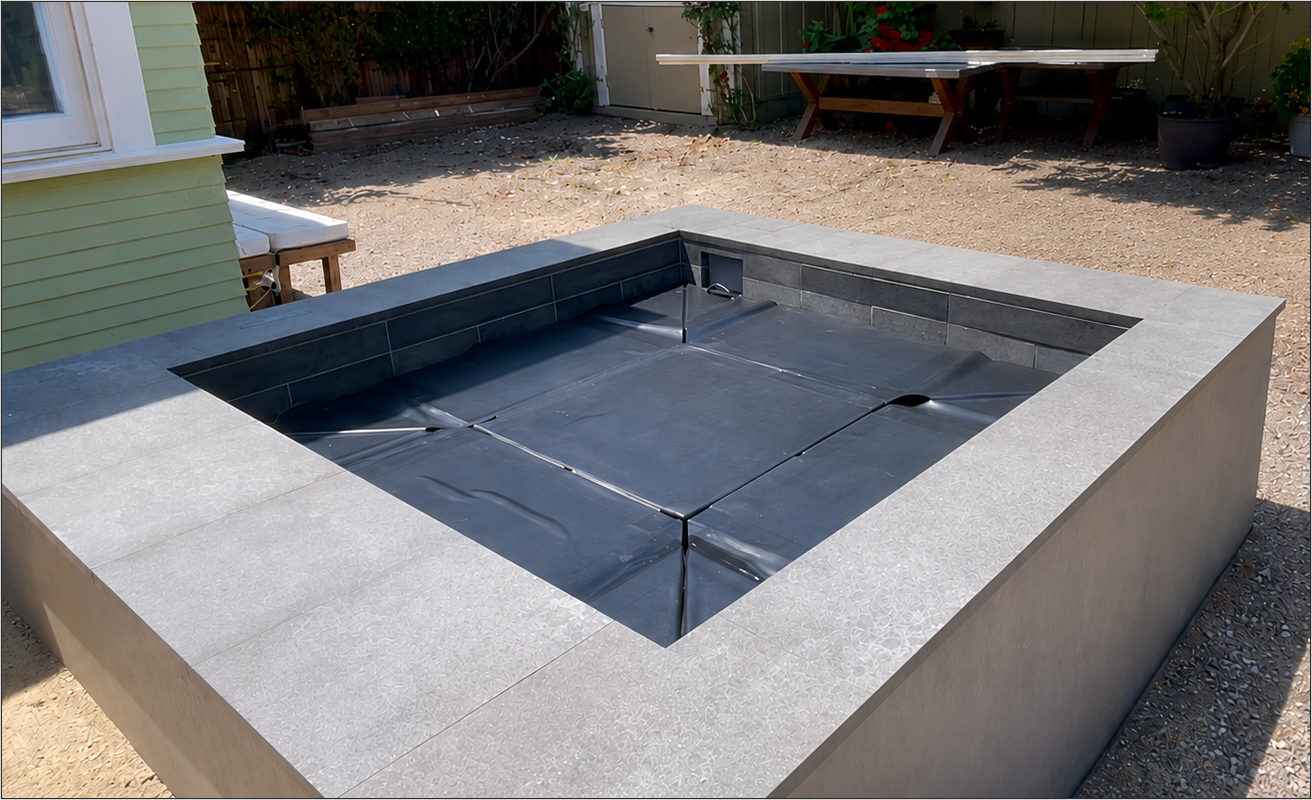
\includegraphics[
        width=5.55in,
        height=2.78in,
        keepaspectratio
    ]{deployed_functional_prototype}
};

\draw[DeepGreen,line width=0.8pt,rounded corners=7pt]
    ($(current page.north west)+(5.16in,-1.61in)$)
    rectangle
    ($(current page.north east)+(-0.42in,-4.47in)$);

\node[
    anchor=north west,
    text=Muted,
    font=\sffamily\fontsize{6.2}{6.9}\selectfont
]
at ($(current page.north west)+(5.18in,-4.54in)$)
{Functional foam model deployed over the sponsor's in-ground spa.};

% Image-strip title
\node[
    anchor=north west,
    text=DeepGreen,
    font=\sffamily\bfseries\fontsize{8.1}{8.8}\selectfont
]
at ($(current page.north west)+(0.43in,-4.78in)$)
{PRODUCT DEVELOPMENT AND FINAL ARCHITECTURE};

% Five-image development strip — CAD-first sequence
% Image 1: topside CAD
\node[anchor=center,inner sep=0pt]
at ($(current page.north west)+(1.47in,-5.73in)$)
{
    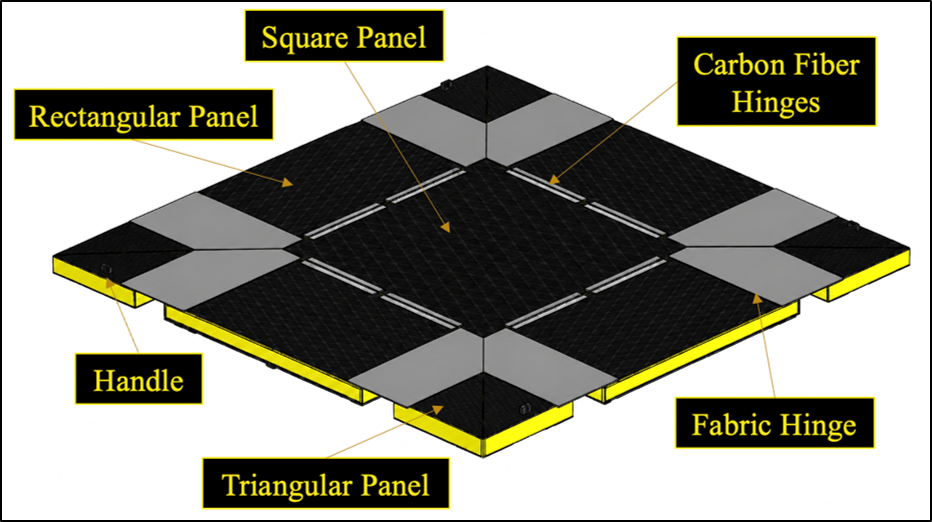
\includegraphics[
        width=1.92in,
        height=1.30in,
        keepaspectratio
    ]{Toro_Cover_topside_Cad}
};
\draw[RuleGray,line width=0.55pt,rounded corners=4pt]
    ($(current page.north west)+(0.43in,-5.04in)$)
    rectangle
    ($(current page.north west)+(2.51in,-6.43in)$);

% Image 2: underside CAD
\node[anchor=center,inner sep=0pt]
at ($(current page.north west)+(3.66in,-5.73in)$)
{
    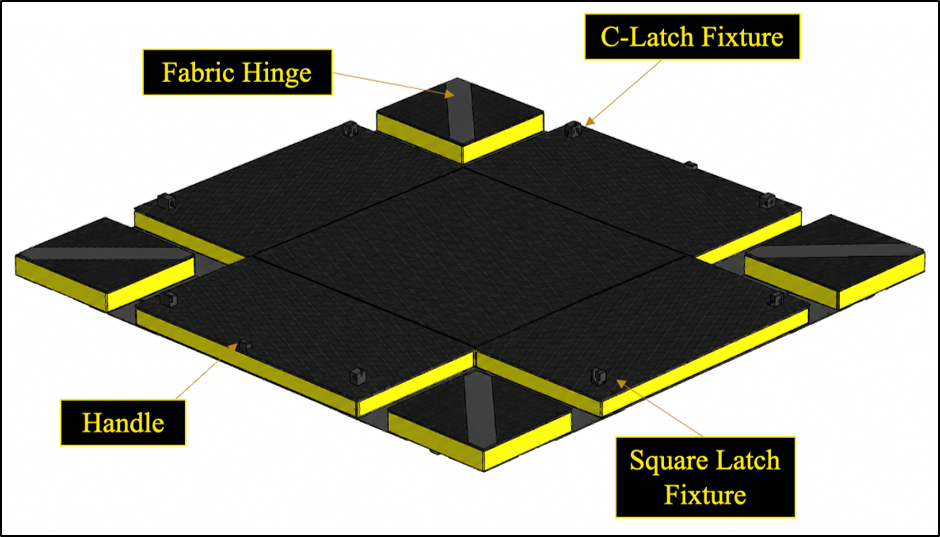
\includegraphics[
        width=1.92in,
        height=1.30in,
        keepaspectratio
    ]{toro_cover_underside_cad}
};
\draw[RuleGray,line width=0.55pt,rounded corners=4pt]
    ($(current page.north west)+(2.62in,-5.04in)$)
    rectangle
    ($(current page.north west)+(4.70in,-6.43in)$);

% Image 3: folded CAD
\node[anchor=center,inner sep=0pt]
at ($(current page.north west)+(5.85in,-5.73in)$)
{
    \includegraphics[
        width=1.92in,
        height=1.30in,
        keepaspectratio
    ]{\detokenize{Toro_Cover_folded Configuration}}
};
\draw[RuleGray,line width=0.55pt,rounded corners=4pt]
    ($(current page.north west)+(4.81in,-5.04in)$)
    rectangle
    ($(current page.north west)+(6.89in,-6.43in)$);

% Image 4: dual-use product concept
\node[anchor=center,inner sep=0pt]
at ($(current page.north west)+(8.04in,-5.73in)$)
{
    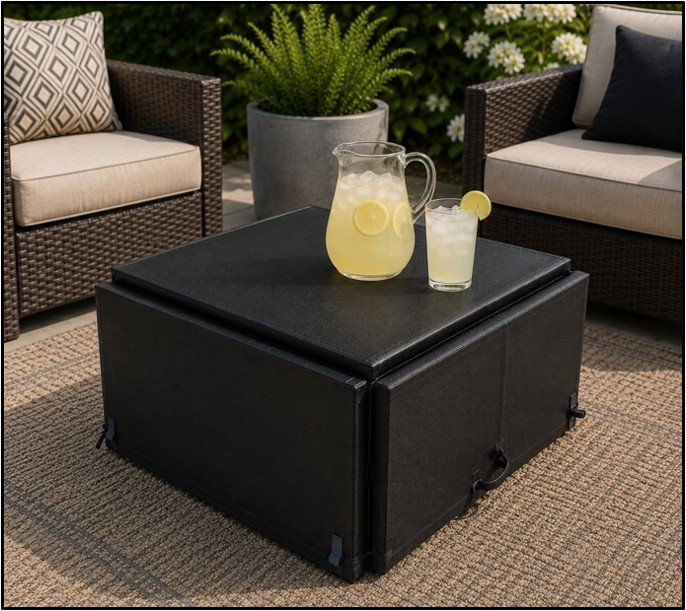
\includegraphics[
        width=1.92in,
        height=1.30in,
        keepaspectratio
    ]{generative_AI_concept_toro_cover_art}
};
\draw[RuleGray,line width=0.55pt,rounded corners=4pt]
    ($(current page.north west)+(7.00in,-5.04in)$)
    rectangle
    ($(current page.north west)+(9.08in,-6.43in)$);

% Image 5: folded foam functional prototype
% The portrait photograph is deliberately clipped to the landscape frame
% so the ottoman fills the card without extending beyond its border.
\begin{scope}
\clip[rounded corners=4pt]
    ($(current page.north west)+(9.19in,-5.04in)$)
    rectangle
    ($(current page.north east)+(-0.43in,-6.43in)$);

% Keep the original image proportions and center it within the existing card.
\node[anchor=center,inner sep=0pt]
at ($(current page.north west)+(9.88in,-5.735in)$)
{
    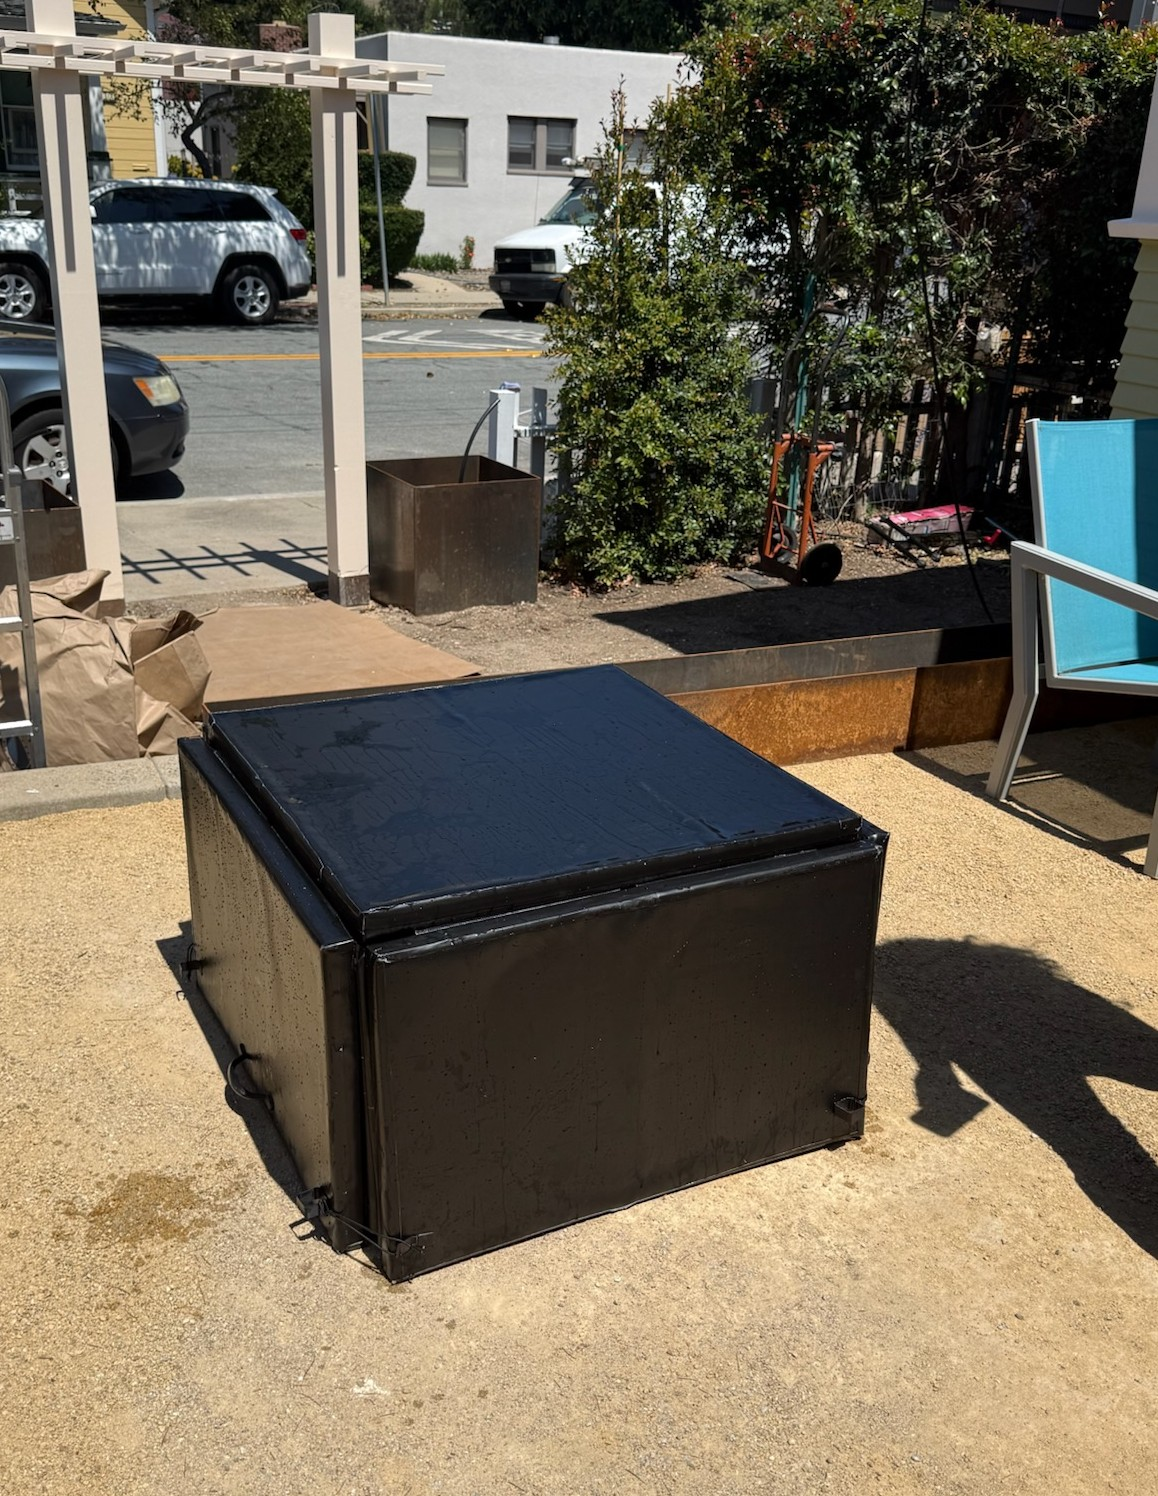
\includegraphics[
        width=1.58in,
        height=1.28in,
        keepaspectratio
    ]{foam_model_folded_backyard_image}
};
\end{scope}

\draw[RuleGray,line width=0.55pt,rounded corners=4pt]
    ($(current page.north west)+(9.19in,-5.04in)$)
    rectangle
    ($(current page.north east)+(-0.43in,-6.43in)$);

% Larger captions
\node[anchor=north,align=center,text width=1.95in,text=Muted,
      font=\sffamily\fontsize{6.8}{7.4}\selectfont]
at ($(current page.north west)+(1.47in,-6.49in)$)
{Topside panel architecture};

\node[anchor=north,align=center,text width=1.95in,text=Muted,
      font=\sffamily\fontsize{6.8}{7.4}\selectfont]
at ($(current page.north west)+(3.66in,-6.49in)$)
{Underside hinge architecture};

\node[anchor=north,align=center,text width=1.95in,text=Muted,
      font=\sffamily\fontsize{6.8}{7.4}\selectfont]
at ($(current page.north west)+(5.85in,-6.49in)$)
{Folded CAD configuration};

\node[anchor=north,align=center,text width=1.95in,text=Muted,
      font=\sffamily\fontsize{6.8}{7.4}\selectfont]
at ($(current page.north west)+(8.04in,-6.49in)$)
{Dual-use product vision};

\node[anchor=north,align=center,text width=1.95in,text=Muted,
      font=\sffamily\fontsize{6.8}{7.4}\selectfont]
at ($(current page.north west)+(9.88in,-6.49in)$)
{Folded foam prototype};

% Page 1 resource bar — centered and non-repeated resources
\fill[Panel,rounded corners=4pt]
    ($(current page.north west)+(0.43in,-7.05in)$)
    rectangle
    ($(current page.north east)+(-0.43in,-7.64in)$);
\draw[RuleGray,line width=0.5pt,rounded corners=4pt]
    ($(current page.north west)+(0.43in,-7.05in)$)
    rectangle
    ($(current page.north east)+(-0.43in,-7.64in)$);

\node[
    anchor=center,
    align=center,
    text=DeepGreen,
    font=\sffamily\bfseries\fontsize{6.9}{7.5}\selectfont
]
at ($(current page.north)+(0,-7.345in)$)
{\href{\ToroDrawingLink}{\faDraftingCompass\ DRAWING PACKAGE}
\hspace{24pt}
\href{\ToroDimensionsLink}{\faImage\ DIMENSION STUDY}
\hspace{24pt}
\href{\ToroProblemLink}{\faFileImage\ PROBLEM STATEMENT}};

% Footer
\node[
    anchor=south west,
    text=white,
    font=\sffamily\bfseries\fontsize{7.1}{7.7}\selectfont
]
at ($(current page.south west)+(0.42in,0.17in)$)
{\hyperlink{composites}{\faArrowLeft\ COMPOSITES}};

\node[
    anchor=south,
    text=white,
    font=\sffamily\fontsize{7.0}{7.6}\selectfont
]
at ($(current page.south)+(0,0.17in)$)
{TORO COVER \hspace{6pt} 1 / 3};

\node[
    anchor=south east,
    text=white,
    font=\sffamily\bfseries\fontsize{7.1}{7.7}\selectfont
]
at ($(current page.south east)+(-0.42in,0.17in)$)
{MANUFACTURING-DRIVEN DESIGN \faArrowRight};

\end{tikzpicture}


% ============================================================
% PAGE 2 — MANUFACTURING-DRIVEN DESIGN
% ============================================================

\clearpage
\thispagestyle{empty}
\hypertarget{toro-manufacturing}{}
\null

\begin{tikzpicture}[remember picture,overlay]

% Background and bars
\fill[white]
    (current page.south west)
    rectangle
    (current page.north east);

\fill[DeepGreen]
    (current page.north west)
    rectangle
    ($(current page.north east)+(0,-0.095in)$);

\fill[PolyGold]
    ($(current page.north west)+(0,-0.095in)$)
    rectangle
    ($(current page.north east)+(0,-0.14in)$);

\fill[DeepGreen]
    (current page.south west)
    rectangle
    ($(current page.south east)+(0,0.36in)$);

\fill[PolyGold]
    ($(current page.south west)+(0,0.36in)$)
    rectangle
    ($(current page.south east)+(0,0.405in)$);

% Header
\node[
    anchor=north west,
    text=PolyGold,
    font=\sffamily\bfseries\fontsize{8.1}{8.7}\selectfont
]
at ($(current page.north west)+(0.42in,-0.39in)$)
{TORO COVER \hspace{5pt}/\hspace{5pt} DESIGN FOR MANUFACTURABILITY};

\node[
    anchor=north west,
    text=DeepGreen,
    font=\bfseries\fontsize{23}{24}\selectfont
]
at ($(current page.north west)+(0.40in,-0.67in)$)
{THE ENVELOPE METHOD};

\node[
    anchor=north west,
    text=Muted,
    font=\sffamily\fontsize{8.7}{9.6}\selectfont
]
at ($(current page.north west)+(0.42in,-1.12in)$)
{A one-layup process developed for unusually thick insulated composite sandwich panels};

\fill[PolyGold]
    ($(current page.north west)+(0.42in,-1.36in)$)
    rectangle
    ($(current page.north west)+(5.30in,-1.315in)$);

% Process explanation
\fill[SoftGold,rounded corners=5pt]
    ($(current page.north west)+(0.42in,-1.61in)$)
    rectangle
    ($(current page.north east)+(-0.42in,-2.90in)$);

\fill[PolyGold]
    ($(current page.north west)+(0.42in,-1.61in)$)
    rectangle
    ($(current page.north west)+(0.52in,-2.90in)$);

\node[
    anchor=north west,
    text=DeepGreen,
    font=\sffamily\bfseries\fontsize{7.9}{8.6}\selectfont
]
at ($(current page.north west)+(0.67in,-1.76in)$)
{PROCESS INNOVATION};

\node[
    anchor=north west,
    align=left,
    text width=9.55in,
    text=Ink,
    font=\fontsize{7.35}{8.75}\selectfont
]
at ($(current page.north west)+(0.67in,-2.02in)$)
{
Weight reduction and insulation were both essential, leading to the selection of an
XPS foam core. Because XPS could not tolerate composite heat-cure temperatures, prepreg
processing was not practical and the panels had to be manufactured by wet layup with a
room-temperature cure. To simplify this process, I waterjet-cut XPS perimeter strips from
excess foam and placed them around each core inside the vacuum enclosure. Under vacuum,
the top and bottom carbon skins met along the panel sides and compressed against this
border, eliminating a separate edge-banding layup and reducing corner pleating.
};

% Workflow title
\node[
    anchor=north west,
    text=DeepGreen,
    font=\sffamily\bfseries\fontsize{8.0}{8.7}\selectfont
]
at ($(current page.north west)+(0.43in,-3.06in)$)
{MANUFACTURING WORKFLOW};

% Row 1 image 1
\node[anchor=center,inner sep=0pt]
at ($(current page.north west)+(2.07in,-4.105in)$)
{
    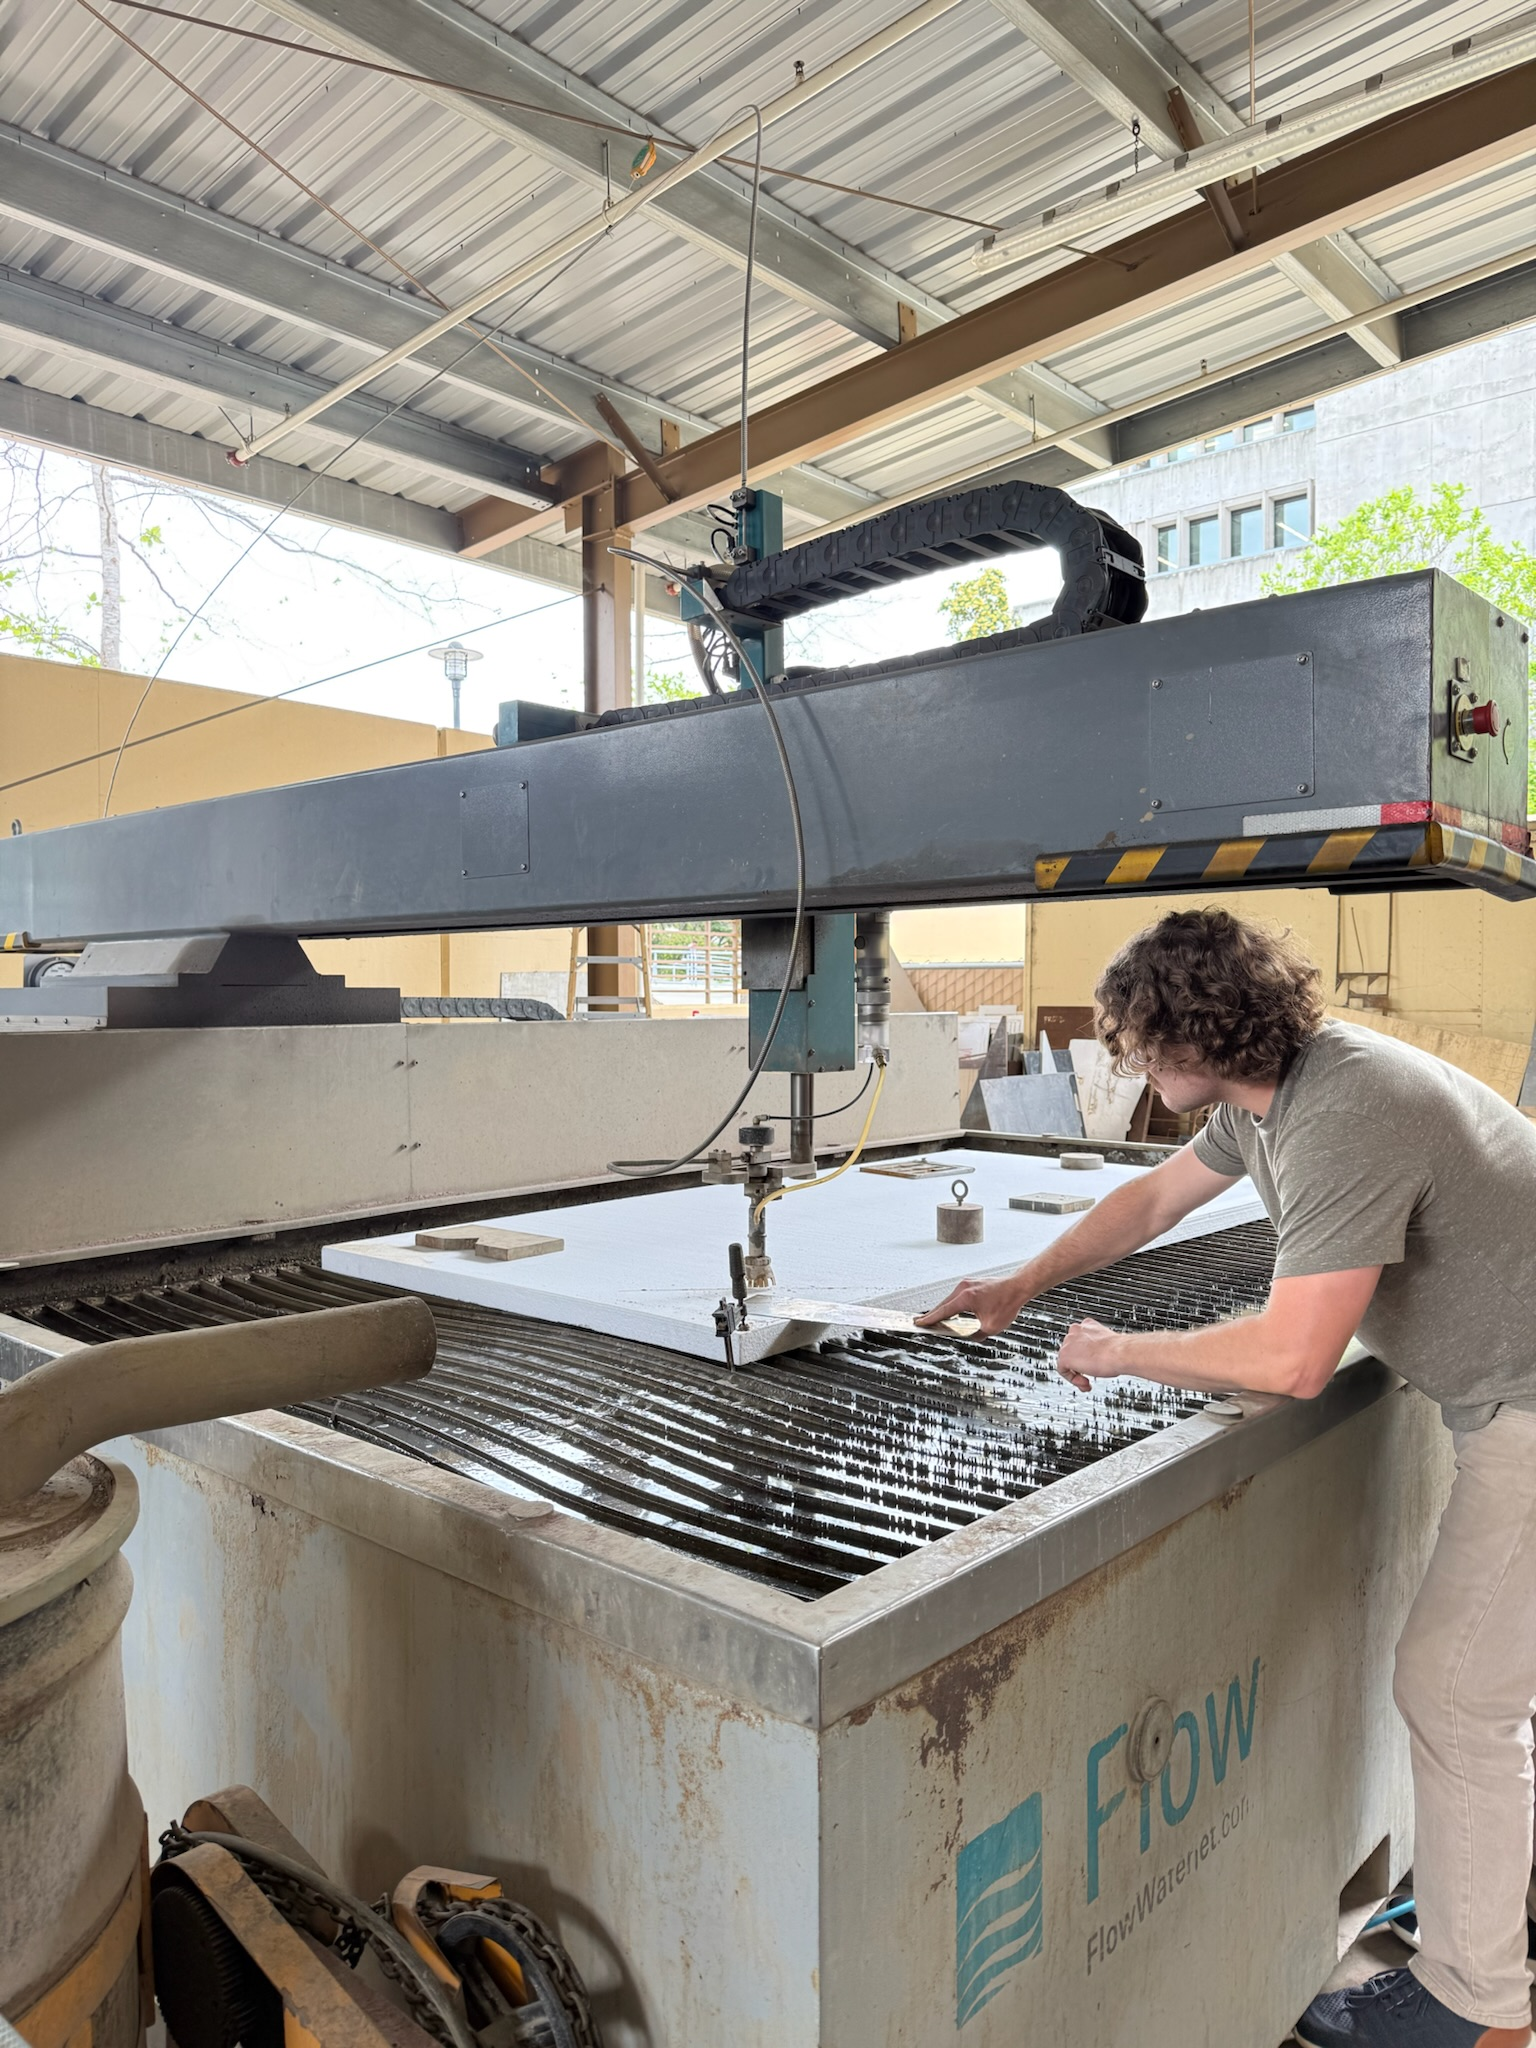
\includegraphics[
        width=3.10in,
        height=1.40in,
        keepaspectratio
    ]{waterjet_foam}
};
\draw[RuleGray,line width=0.55pt,rounded corners=4pt]
    ($(current page.north west)+(0.43in,-3.36in)$)
    rectangle
    ($(current page.north west)+(3.71in,-4.85in)$);

% Row 1 image 2
\node[anchor=center,inner sep=0pt]
at ($(current page.north west)+(5.50in,-4.105in)$)
{
    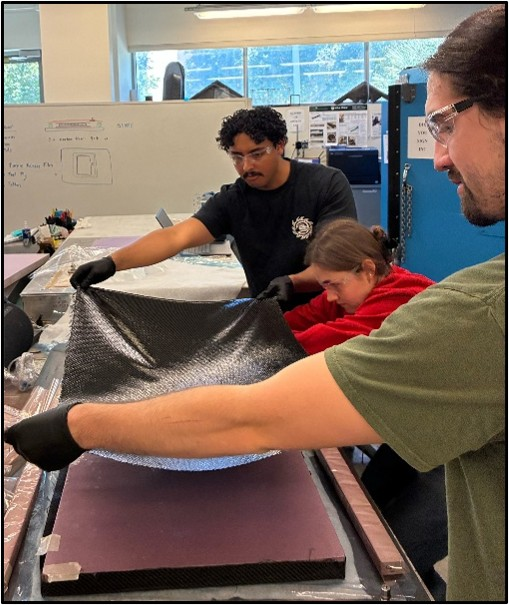
\includegraphics[
        width=3.10in,
        height=1.40in,
        keepaspectratio
    ]{group_layup}
};
\draw[RuleGray,line width=0.55pt,rounded corners=4pt]
    ($(current page.north west)+(3.86in,-3.36in)$)
    rectangle
    ($(current page.north west)+(7.14in,-4.85in)$);

% Row 1 image 3
\node[anchor=center,inner sep=0pt]
at ($(current page.north west)+(8.935in,-4.105in)$)
{
    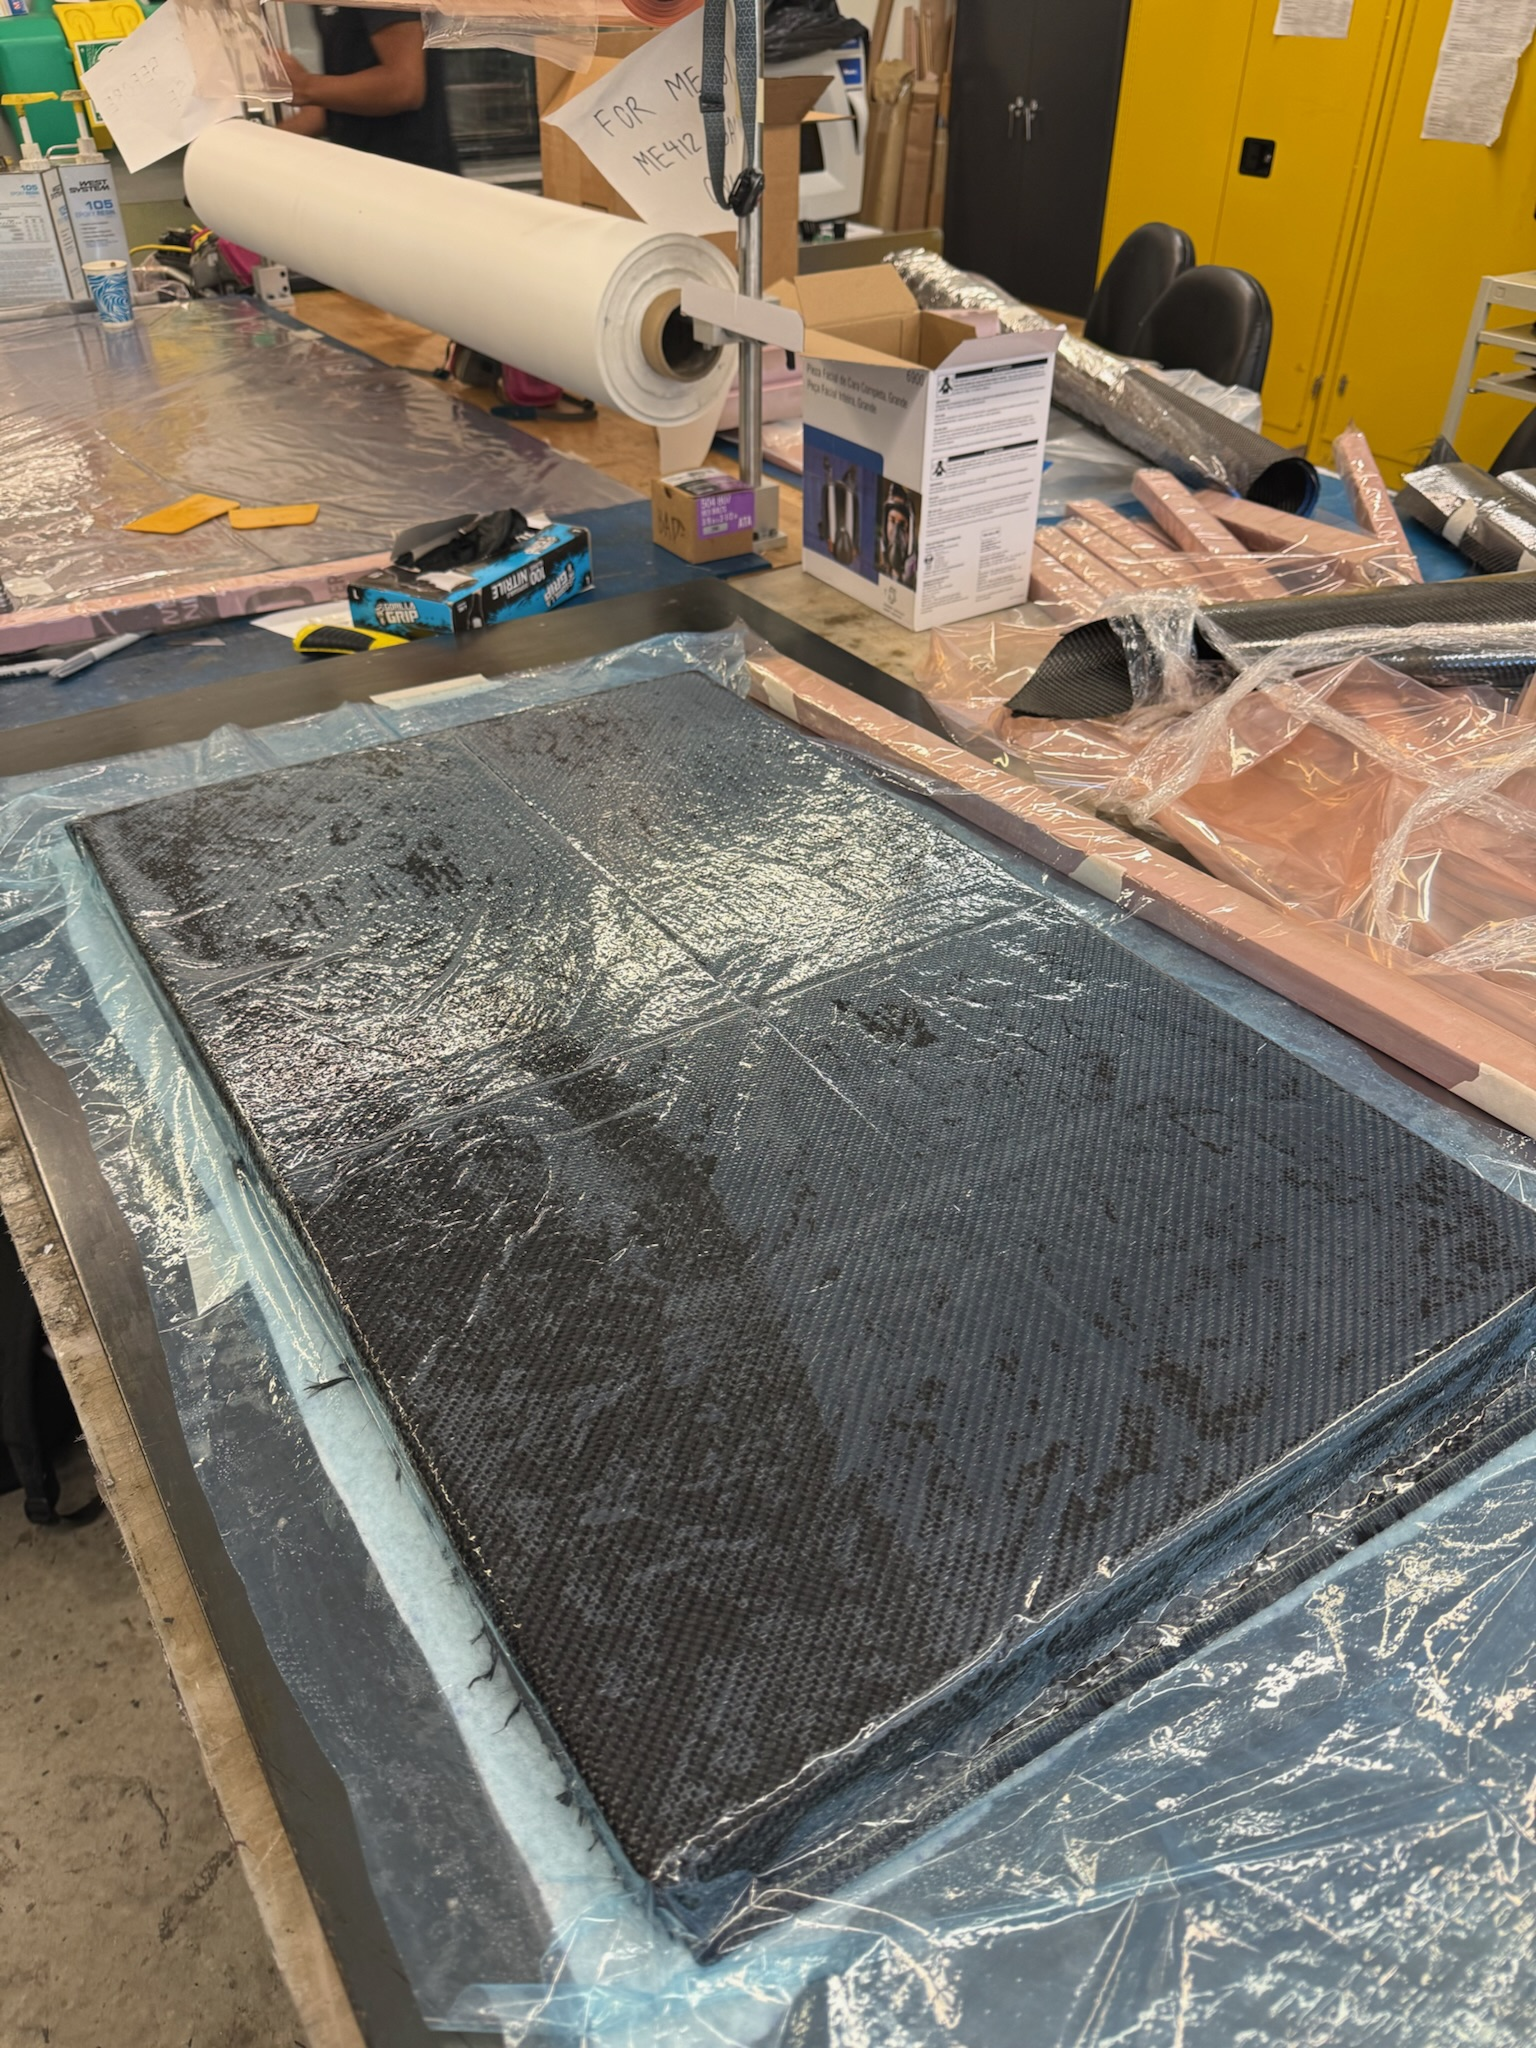
\includegraphics[
        width=3.10in,
        height=1.40in,
        keepaspectratio
    ]{blue_perforrated_film_layup}
};
\draw[RuleGray,line width=0.55pt,rounded corners=4pt]
    ($(current page.north west)+(7.29in,-3.36in)$)
    rectangle
    ($(current page.north east)+(-0.42in,-4.85in)$);

% Row 1 captions
\node[anchor=north,text=Muted,font=\sffamily\fontsize{6.7}{7.3}\selectfont]
at ($(current page.north west)+(2.07in,-4.90in)$)
{1. Waterjet-cut core and perimeter geometry};

\node[anchor=north,text=Muted,font=\sffamily\fontsize{6.7}{7.3}\selectfont]
at ($(current page.north west)+(5.50in,-4.90in)$)
{2. Team wet layup under my process guidance};

\node[anchor=north,text=Muted,font=\sffamily\fontsize{6.7}{7.3}\selectfont]
at ($(current page.north west)+(8.935in,-4.90in)$)
{3. Perforated film, breather, and vacuum enclosure};

% Row 2 image 1
\node[anchor=center,inner sep=0pt]
at ($(current page.north west)+(2.07in,-5.875in)$)
{
    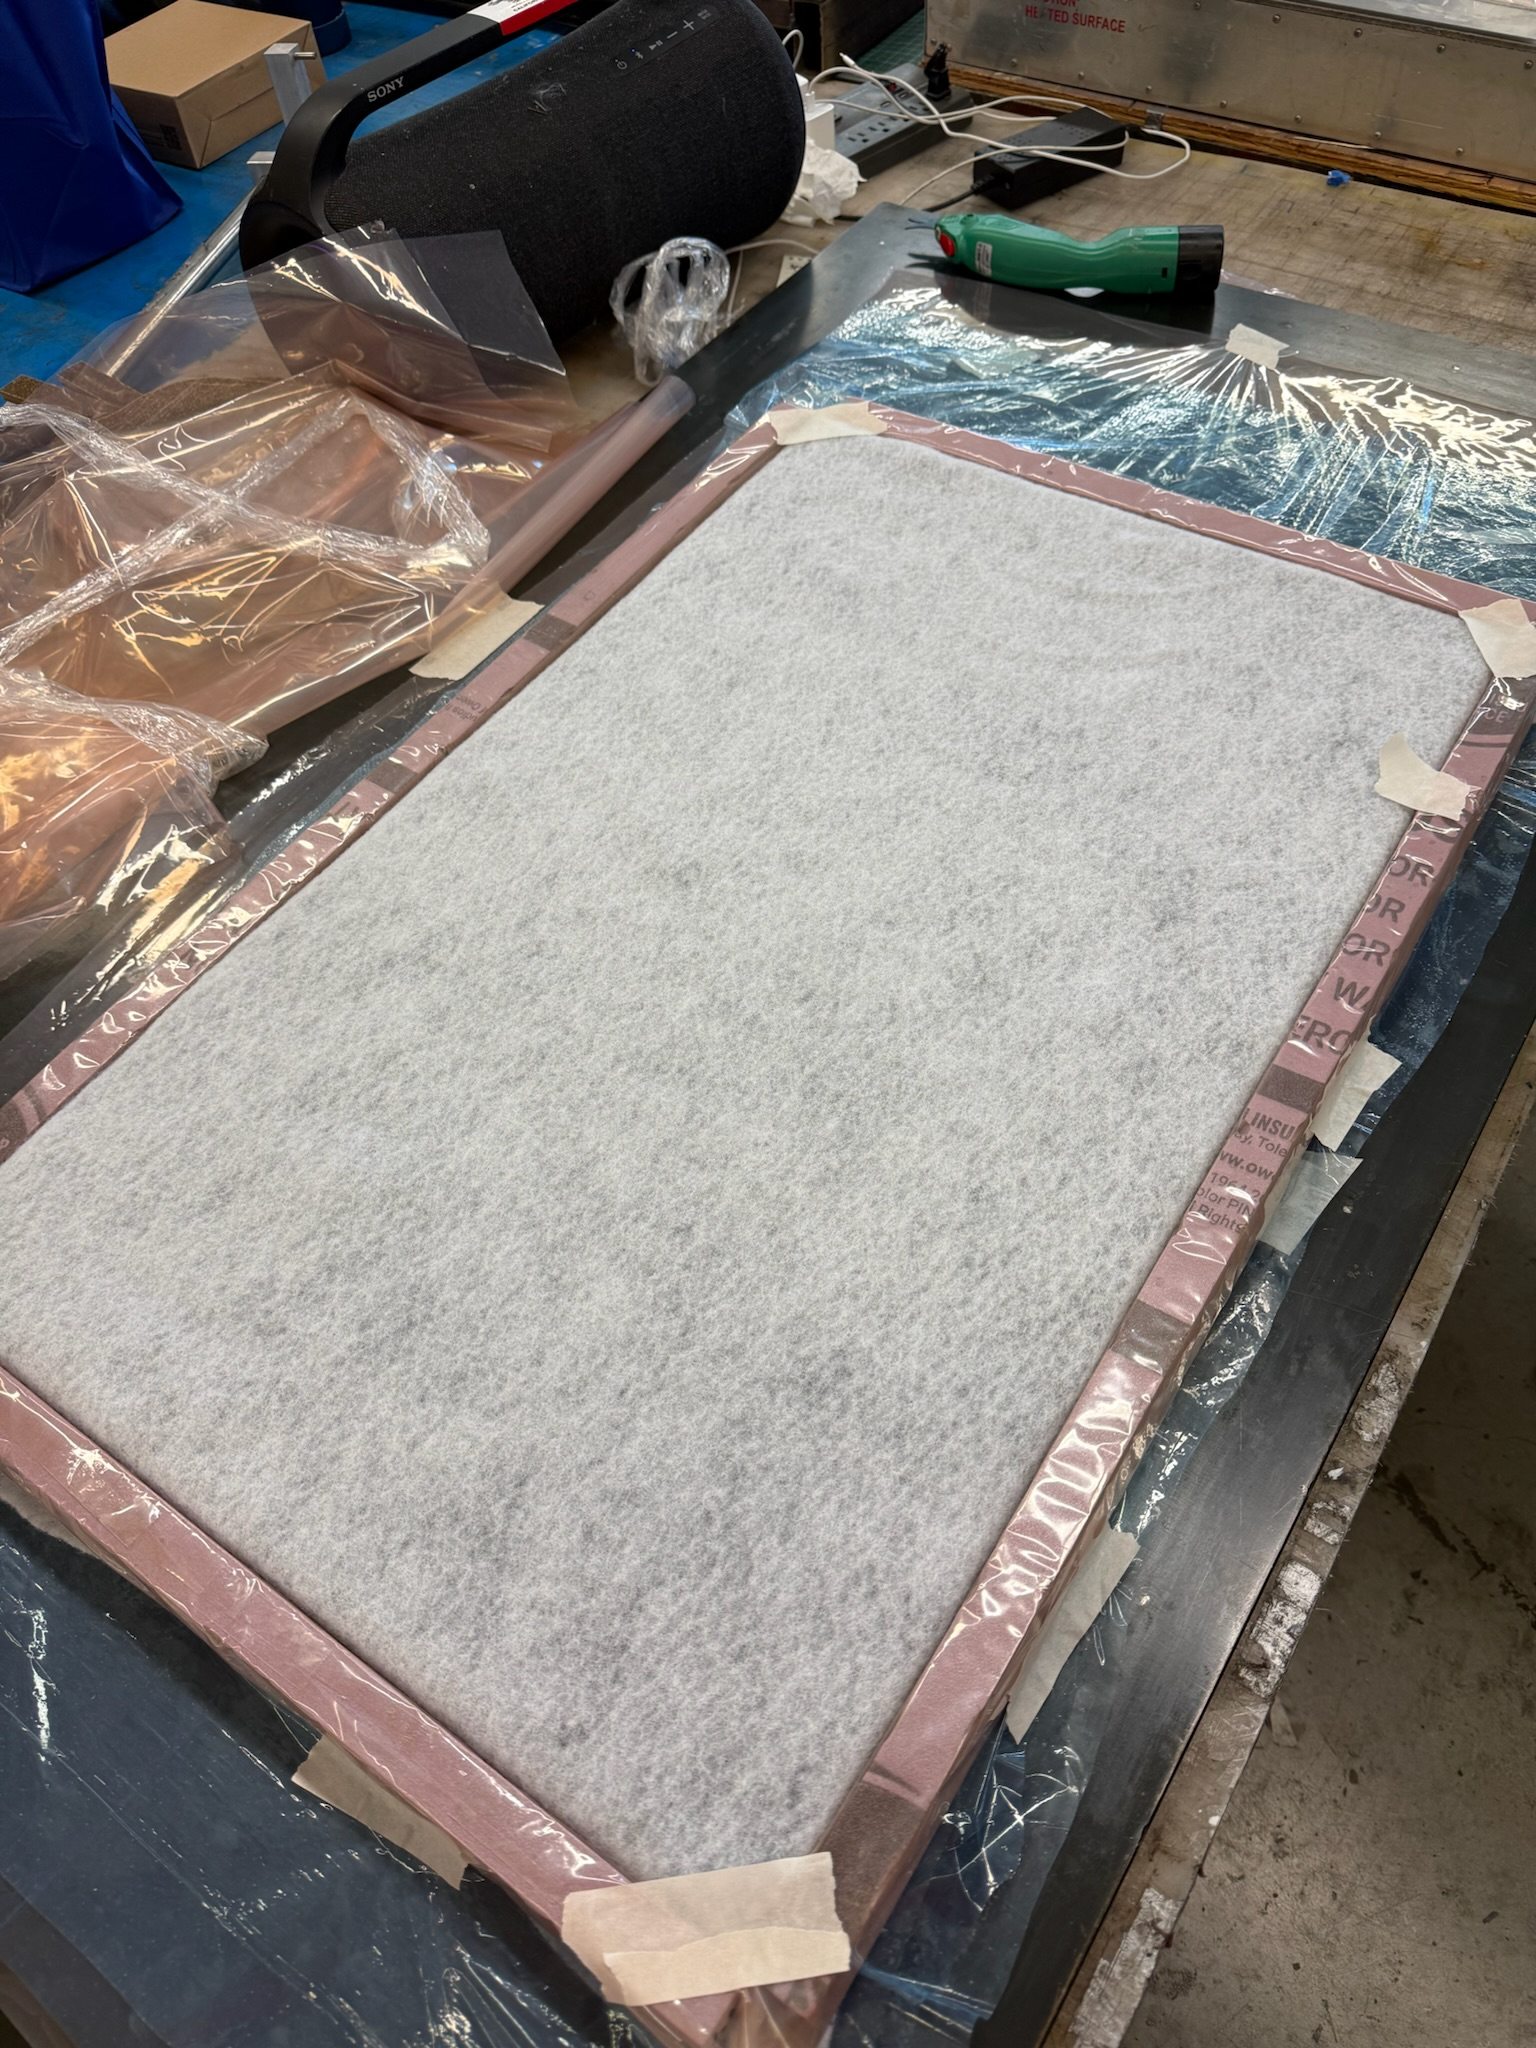
\includegraphics[
        width=3.10in,
        height=1.40in,
        keepaspectratio
    ]{completed_layup}
};
\draw[RuleGray,line width=0.55pt,rounded corners=4pt]
    ($(current page.north west)+(0.43in,-5.13in)$)
    rectangle
    ($(current page.north west)+(3.71in,-6.62in)$);

% Row 2 image 2 — oven chamber used only as a reliable vacuum enclosure; no heat applied
\node[anchor=center,inner sep=0pt]
at ($(current page.north west)+(5.50in,-5.875in)$)
{
    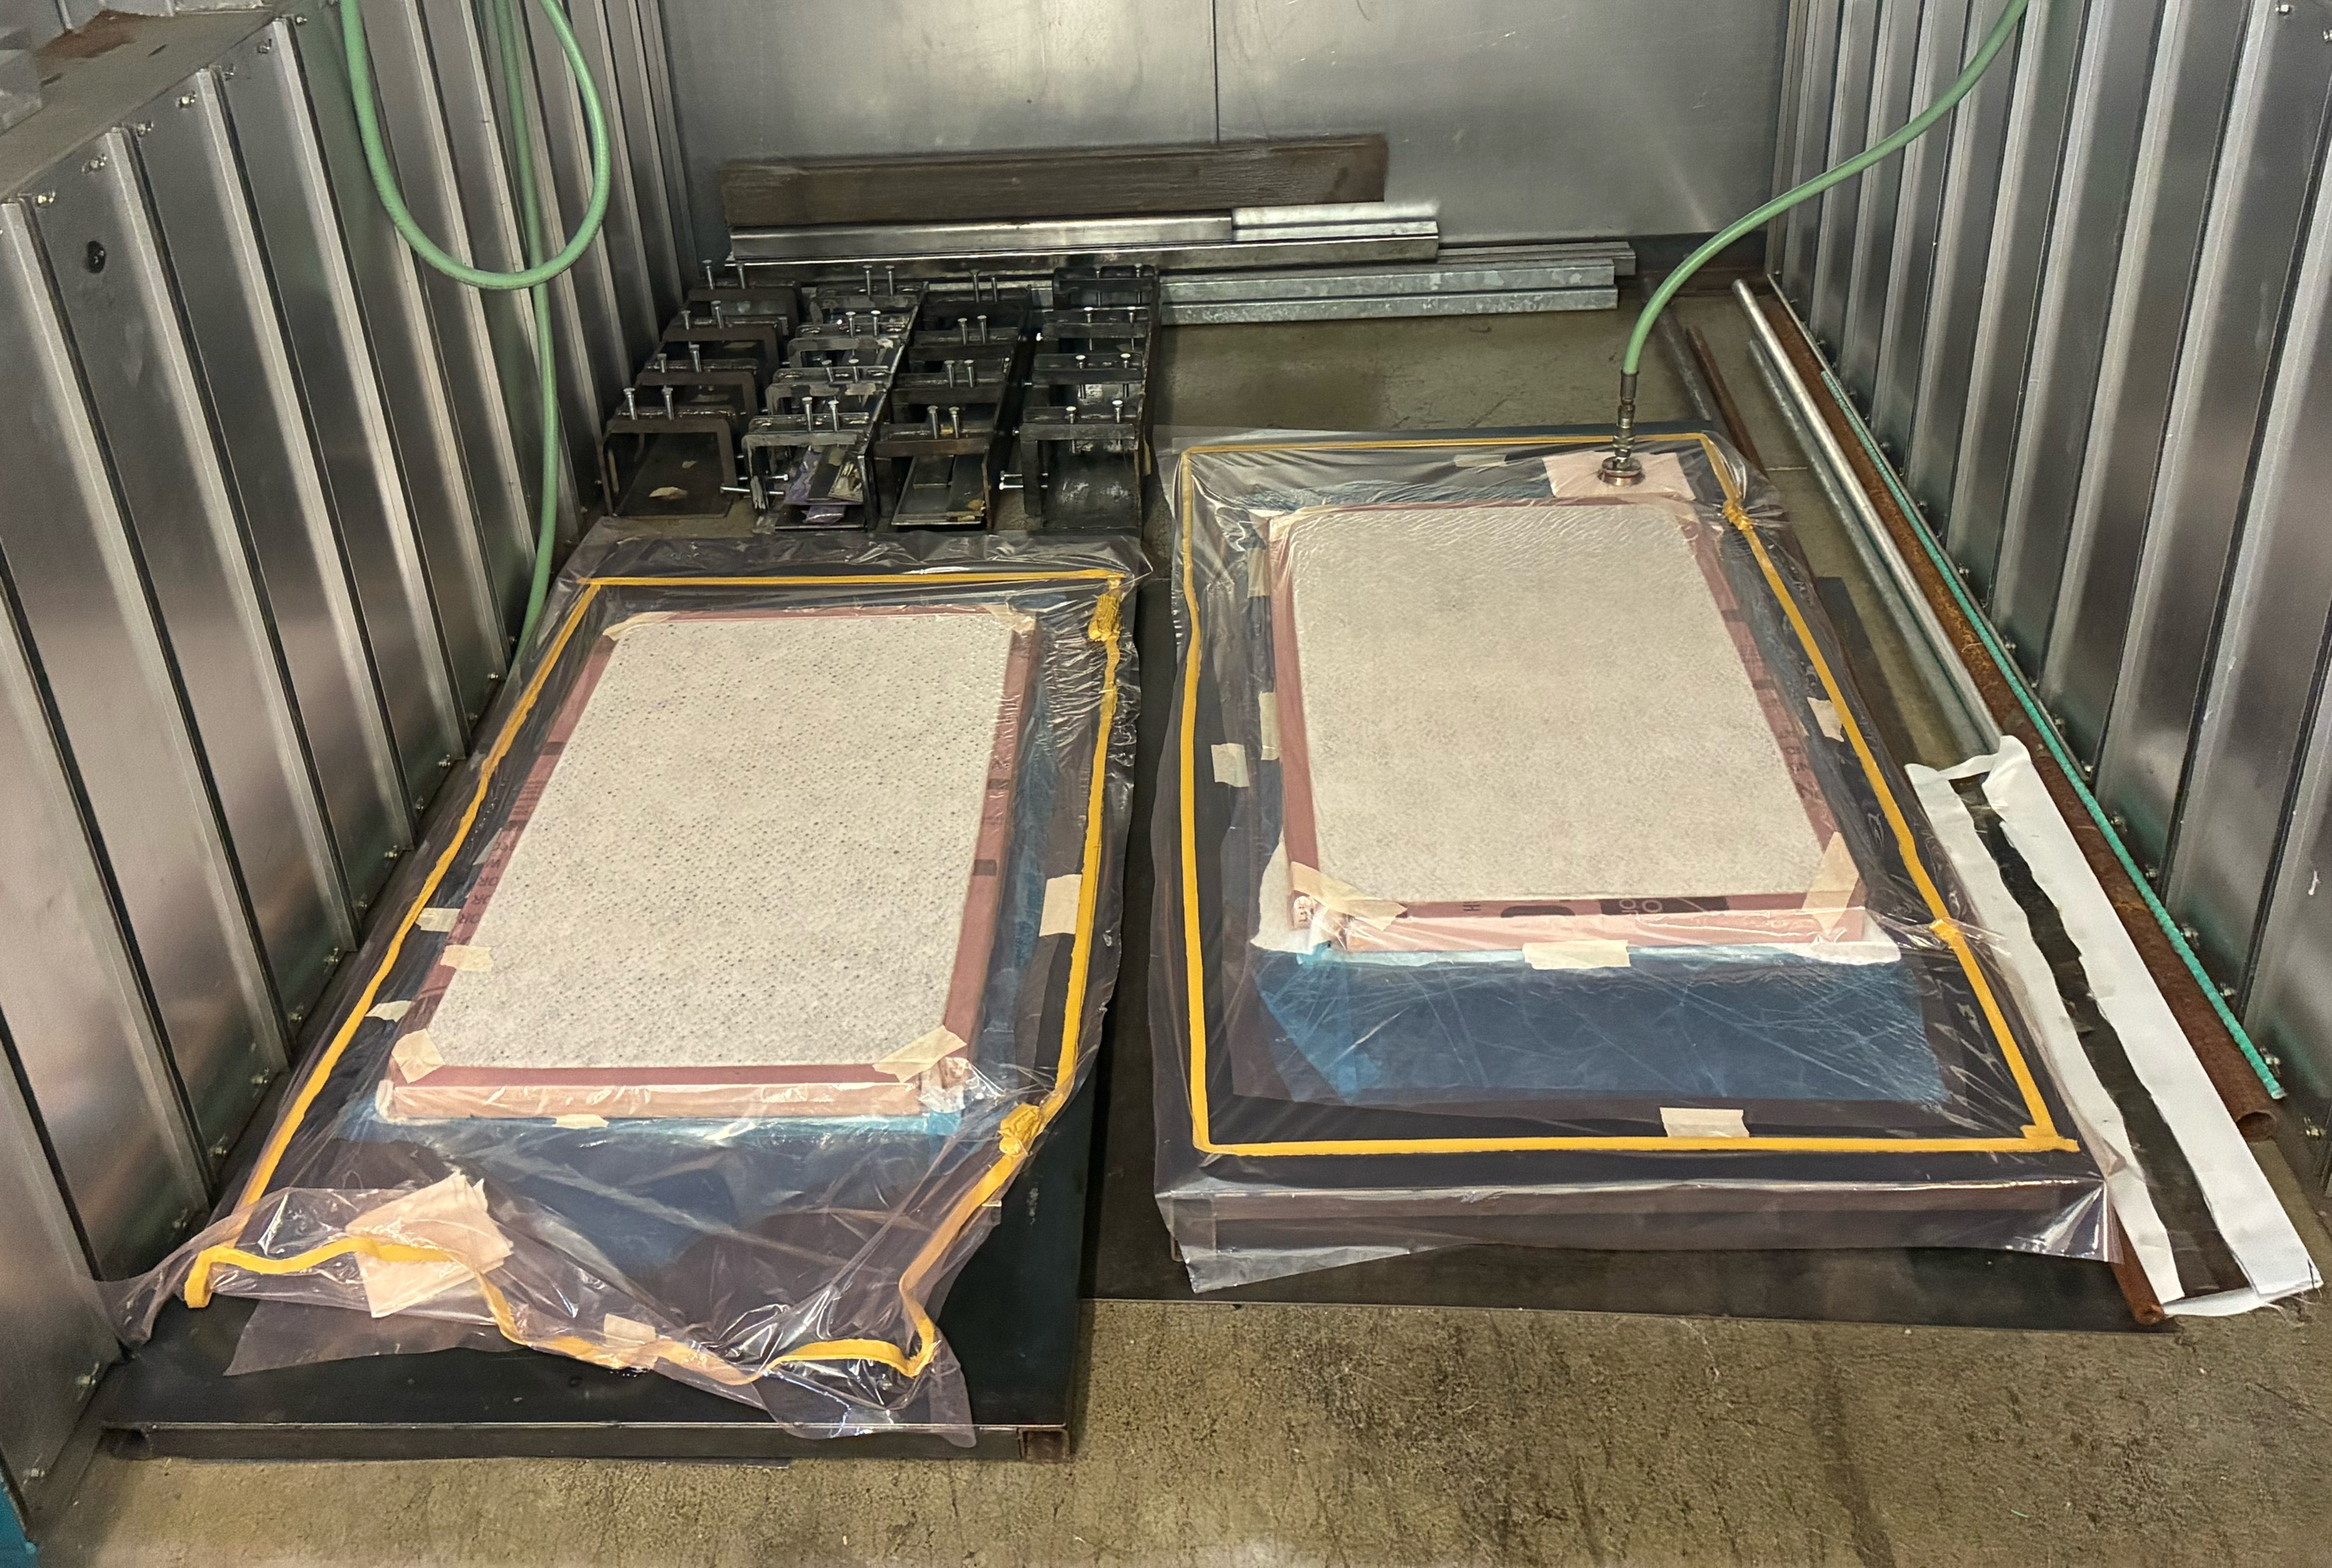
\includegraphics[
        width=3.10in,
        height=1.40in,
        keepaspectratio
    ]{layups_in_composite_oven_under_vacuumPressure}
};
\draw[RuleGray,line width=0.55pt,rounded corners=4pt]
    ($(current page.north west)+(3.86in,-5.13in)$)
    rectangle
    ($(current page.north west)+(7.14in,-6.62in)$);

% Row 2 image 3
\node[anchor=center,inner sep=0pt]
at ($(current page.north west)+(8.935in,-5.875in)$)
{
    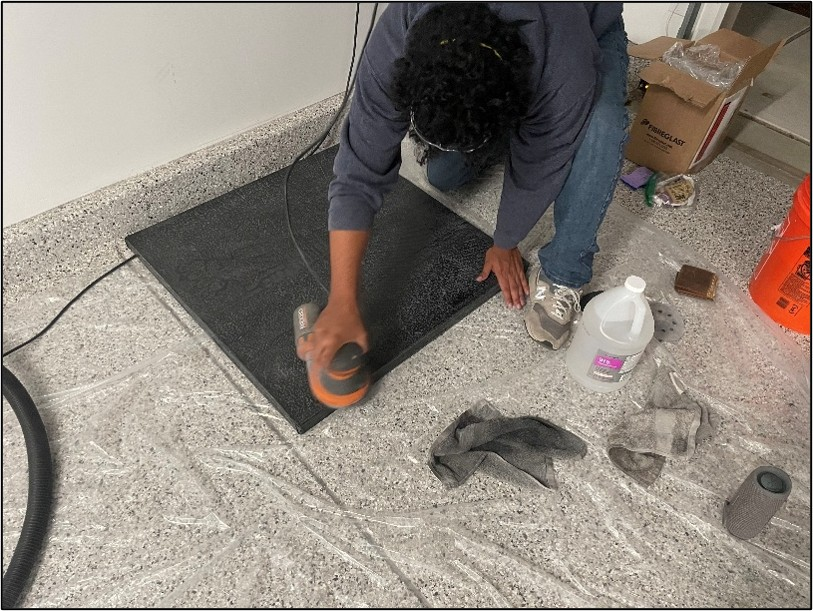
\includegraphics[
        width=3.10in,
        height=1.40in,
        keepaspectratio
    ]{garage_sanding}
};
\draw[RuleGray,line width=0.55pt,rounded corners=4pt]
    ($(current page.north west)+(7.29in,-5.13in)$)
    rectangle
    ($(current page.north east)+(-0.42in,-6.62in)$);

% Row 2 captions
\node[anchor=north,text=Muted,font=\sffamily\fontsize{6.7}{7.3}\selectfont]
at ($(current page.north west)+(2.07in,-6.67in)$)
{4. Fully saturated carbon skin and foam sandwich};

\node[anchor=north,text=Muted,font=\sffamily\fontsize{6.7}{7.3}\selectfont]
at ($(current page.north west)+(5.50in,-6.67in)$)
{5. Room-temperature cure under continuous vacuum};

\node[anchor=north,text=Muted,font=\sffamily\fontsize{6.7}{7.3}\selectfont]
at ($(current page.north west)+(8.935in,-6.67in)$)
{6. Post-processing and surface preparation};

% Bottom callouts
\fill[Panel,rounded corners=4pt]
    ($(current page.north west)+(0.43in,-6.95in)$)
    rectangle
    ($(current page.north west)+(5.48in,-7.60in)$);

\draw[RuleGray,line width=0.55pt,rounded corners=4pt]
    ($(current page.north west)+(0.43in,-6.95in)$)
    rectangle
    ($(current page.north west)+(5.48in,-7.60in)$);

\node[
    anchor=north west,
    text=DeepGreen,
    font=\sffamily\bfseries\fontsize{7.0}{7.6}\selectfont
]
at ($(current page.north west)+(0.63in,-7.08in)$)
{FROM THREE LAYUPS TO ONE};

\node[
    anchor=north west,
    align=left,
    text width=4.56in,
    text=Ink,
    font=\fontsize{6.45}{7.45}\selectfont
]
at ($(current page.north west)+(0.63in,-7.29in)$)
{
The Envelope Method reduced labor, cure cycles, handling,
alignment risk, and time spent forming numerous vacuum-bag
pleats around the 1.5-inch-thick XPS panels.
};

\fill[Panel,rounded corners=4pt]
    ($(current page.north west)+(5.68in,-6.95in)$)
    rectangle
    ($(current page.north east)+(-0.42in,-7.60in)$);

\draw[RuleGray,line width=0.55pt,rounded corners=4pt]
    ($(current page.north west)+(5.68in,-6.95in)$)
    rectangle
    ($(current page.north east)+(-0.42in,-7.60in)$);

\node[
    anchor=north west,
    text=DeepGreen,
    font=\sffamily\bfseries\fontsize{7.0}{7.6}\selectfont
]
at ($(current page.north west)+(5.88in,-7.08in)$)
{WHY SURFACE-BONDED HARDWARE};

\node[
    anchor=north west,
    align=left,
    text width=4.55in,
    text=Ink,
    font=\fontsize{6.45}{7.45}\selectfont
]
at ($(current page.north west)+(5.88in,-7.29in)$)
{
Adhesively bonded hinges and fixtures preserved the clean
composite exterior and avoided drilled inserts, foam-core
crushing, added stress concentrations, and new leak paths.
};


% Footer
\node[
    anchor=south west,
    text=white,
    font=\sffamily\bfseries\fontsize{7.1}{7.7}\selectfont
]
at ($(current page.south west)+(0.42in,0.17in)$)
{\faArrowLeft\ PRODUCT ARCHITECTURE};

\node[
    anchor=south,
    text=white,
    font=\sffamily\fontsize{7.0}{7.6}\selectfont
]
at ($(current page.south)+(0,0.17in)$)
{TORO COVER \hspace{6pt} 2 / 3};

\node[
    anchor=south east,
    text=white,
    font=\sffamily\bfseries\fontsize{7.1}{7.7}\selectfont
]
at ($(current page.south east)+(-0.42in,0.17in)$)
{VALIDATION \& TAKEAWAYS \faArrowRight};

\end{tikzpicture}


% ============================================================
% PAGE 3 — FINISHING, VALIDATION, AND TAKEAWAYS
% ============================================================

\clearpage
\thispagestyle{empty}
\hypertarget{toro-results}{}
\null

\begin{tikzpicture}[remember picture,overlay]

% Background and bars
\fill[white]
    (current page.south west)
    rectangle
    (current page.north east);

\fill[DeepGreen]
    (current page.north west)
    rectangle
    ($(current page.north east)+(0,-0.095in)$);

\fill[PolyGold]
    ($(current page.north west)+(0,-0.095in)$)
    rectangle
    ($(current page.north east)+(0,-0.14in)$);

\fill[DeepGreen]
    (current page.south west)
    rectangle
    ($(current page.south east)+(0,0.36in)$);

\fill[PolyGold]
    ($(current page.south west)+(0,0.36in)$)
    rectangle
    ($(current page.south east)+(0,0.405in)$);

% Header
\node[
    anchor=north west,
    text=PolyGold,
    font=\sffamily\bfseries\fontsize{8.1}{8.7}\selectfont
]
at ($(current page.north west)+(0.42in,-0.39in)$)
{TORO COVER \hspace{5pt}/\hspace{5pt} VALIDATION AND ENGINEERING TAKEAWAYS};

\node[
    anchor=north west,
    text=DeepGreen,
    font=\bfseries\fontsize{22.5}{23.5}\selectfont
]
at ($(current page.north west)+(0.40in,-0.67in)$)
{FROM PROTOTYPE TO PRODUCT PATHWAY};

\node[
    anchor=north west,
    text=Muted,
    font=\sffamily\fontsize{8.7}{9.6}\selectfont
]
at ($(current page.north west)+(0.42in,-1.12in)$)
{Environmental protection, usability testing, scope decisions, and lessons from technical leadership};

\fill[PolyGold]
    ($(current page.north west)+(0.42in,-1.36in)$)
    rectangle
    ($(current page.north west)+(5.8in,-1.315in)$);

% Finishing title
\node[
    anchor=north west,
    text=DeepGreen,
    font=\sffamily\bfseries\fontsize{8.0}{8.7}\selectfont
]
at ($(current page.north west)+(0.43in,-1.62in)$)
{OUTDOOR FINISHING AND ENVIRONMENTAL PROTECTION};

% Image 1
\node[anchor=center,inner sep=0pt]
at ($(current page.north west)+(1.705in,-2.655in)$)
{
    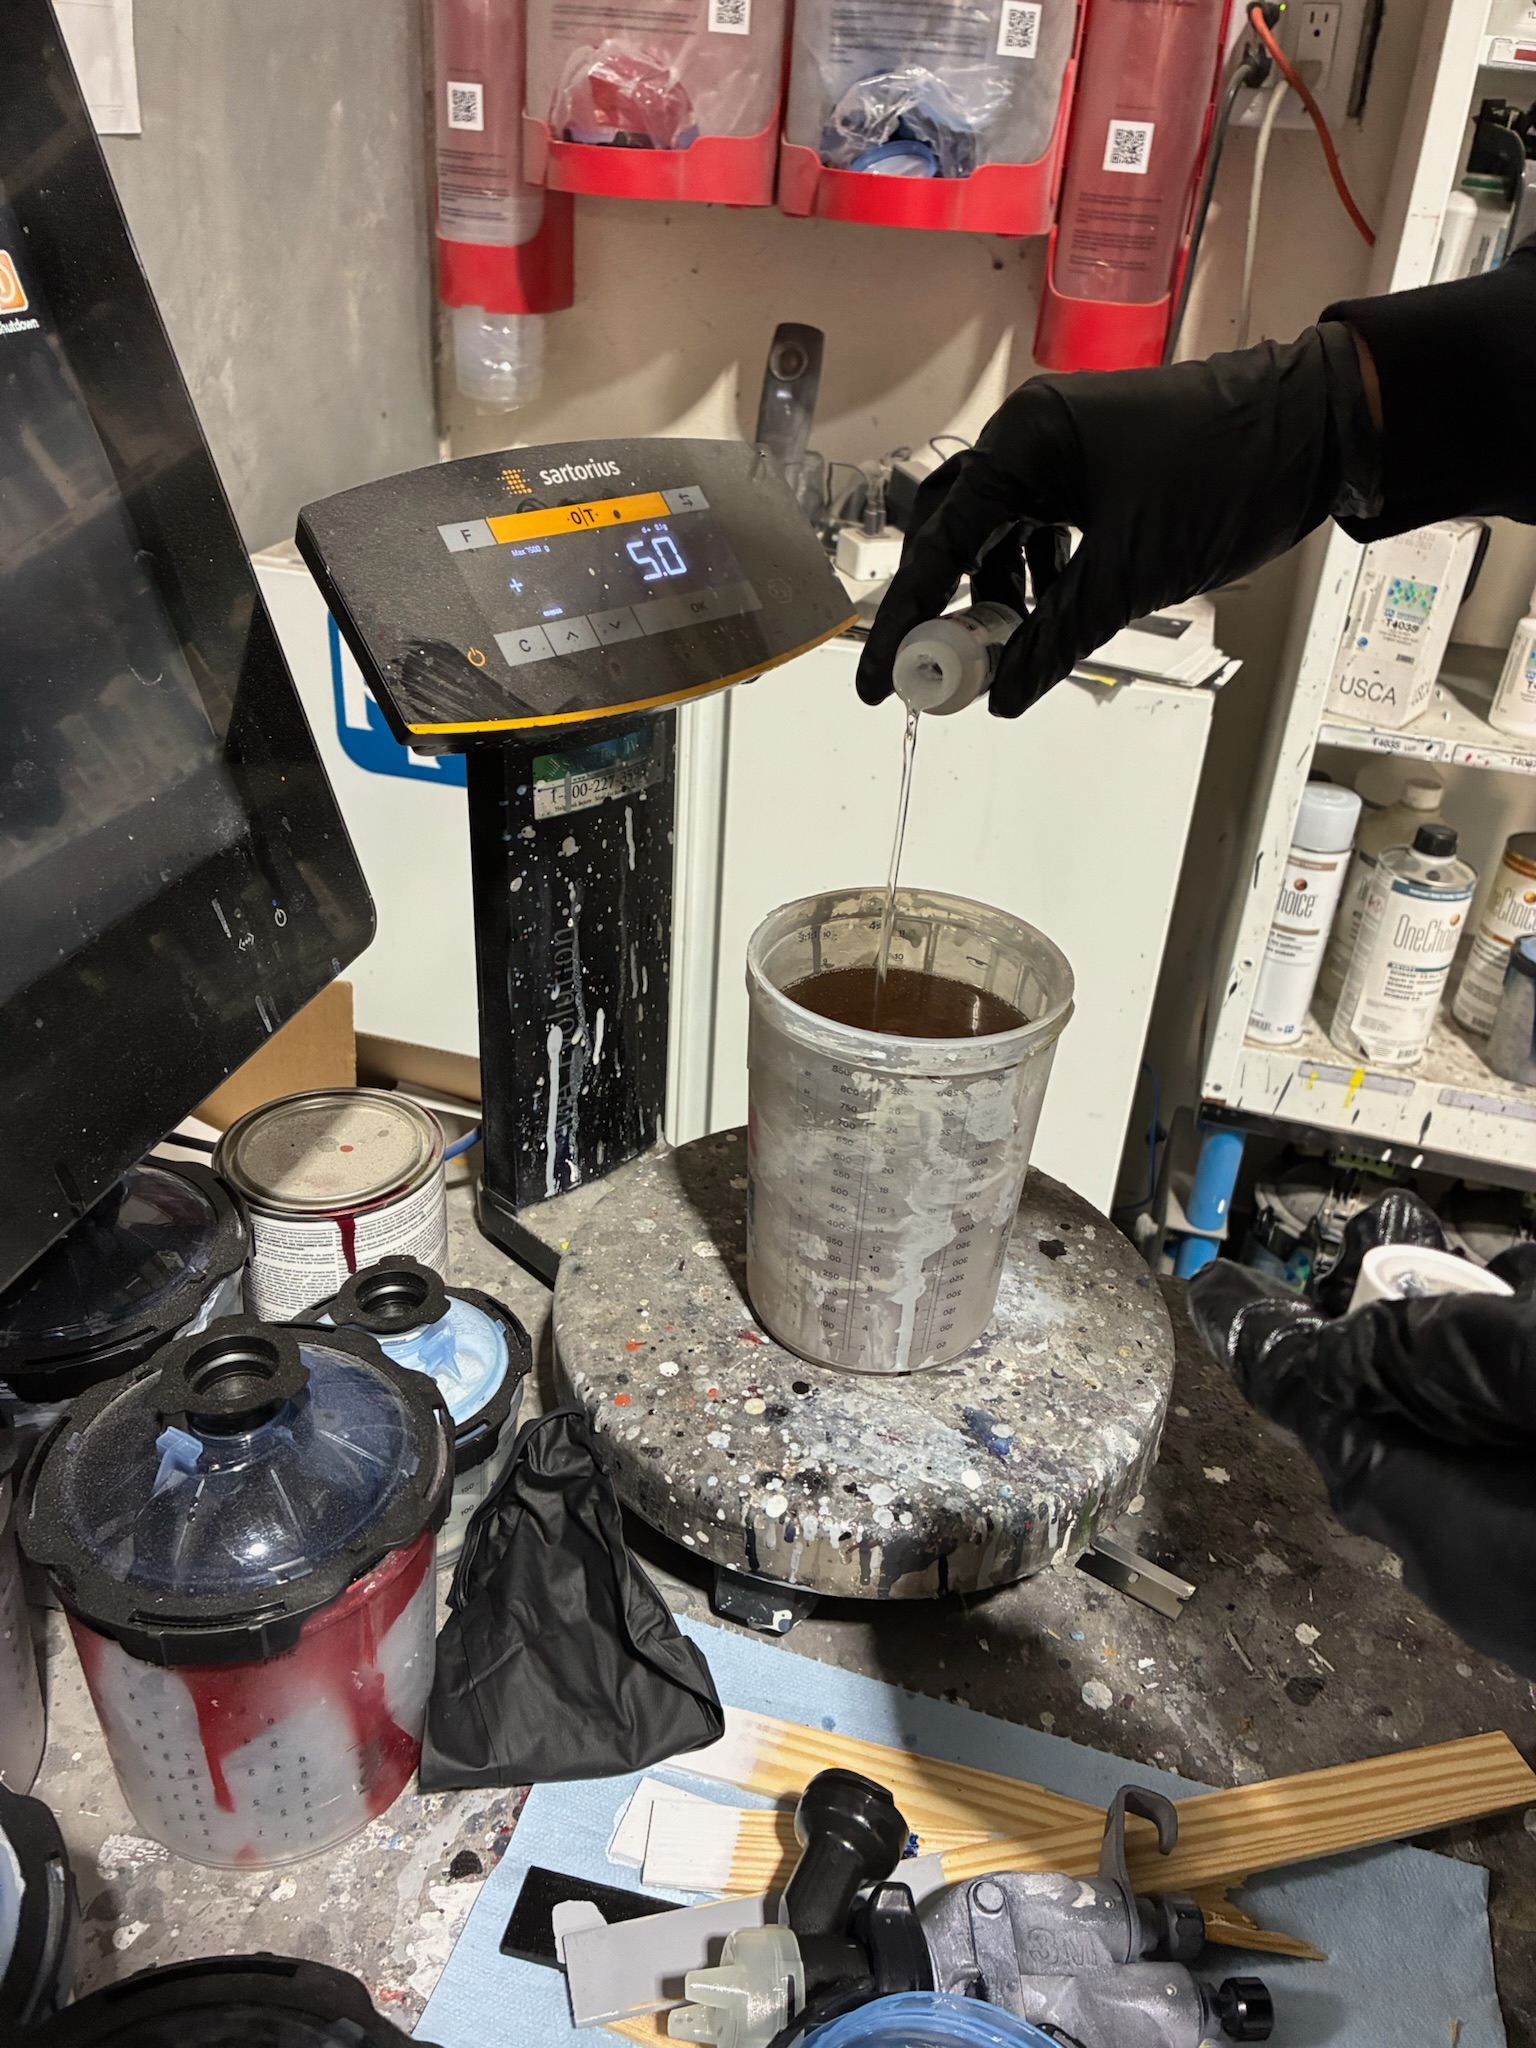
\includegraphics[
        width=2.35in,
        height=1.40in,
        keepaspectratio
    ]{spray_topcoat_prep}
};
\draw[RuleGray,line width=0.55pt,rounded corners=4pt]
    ($(current page.north west)+(0.43in,-1.91in)$)
    rectangle
    ($(current page.north west)+(2.98in,-3.40in)$);

% Image 2
\node[anchor=center,inner sep=0pt]
at ($(current page.north west)+(4.375in,-2.655in)$)
{
    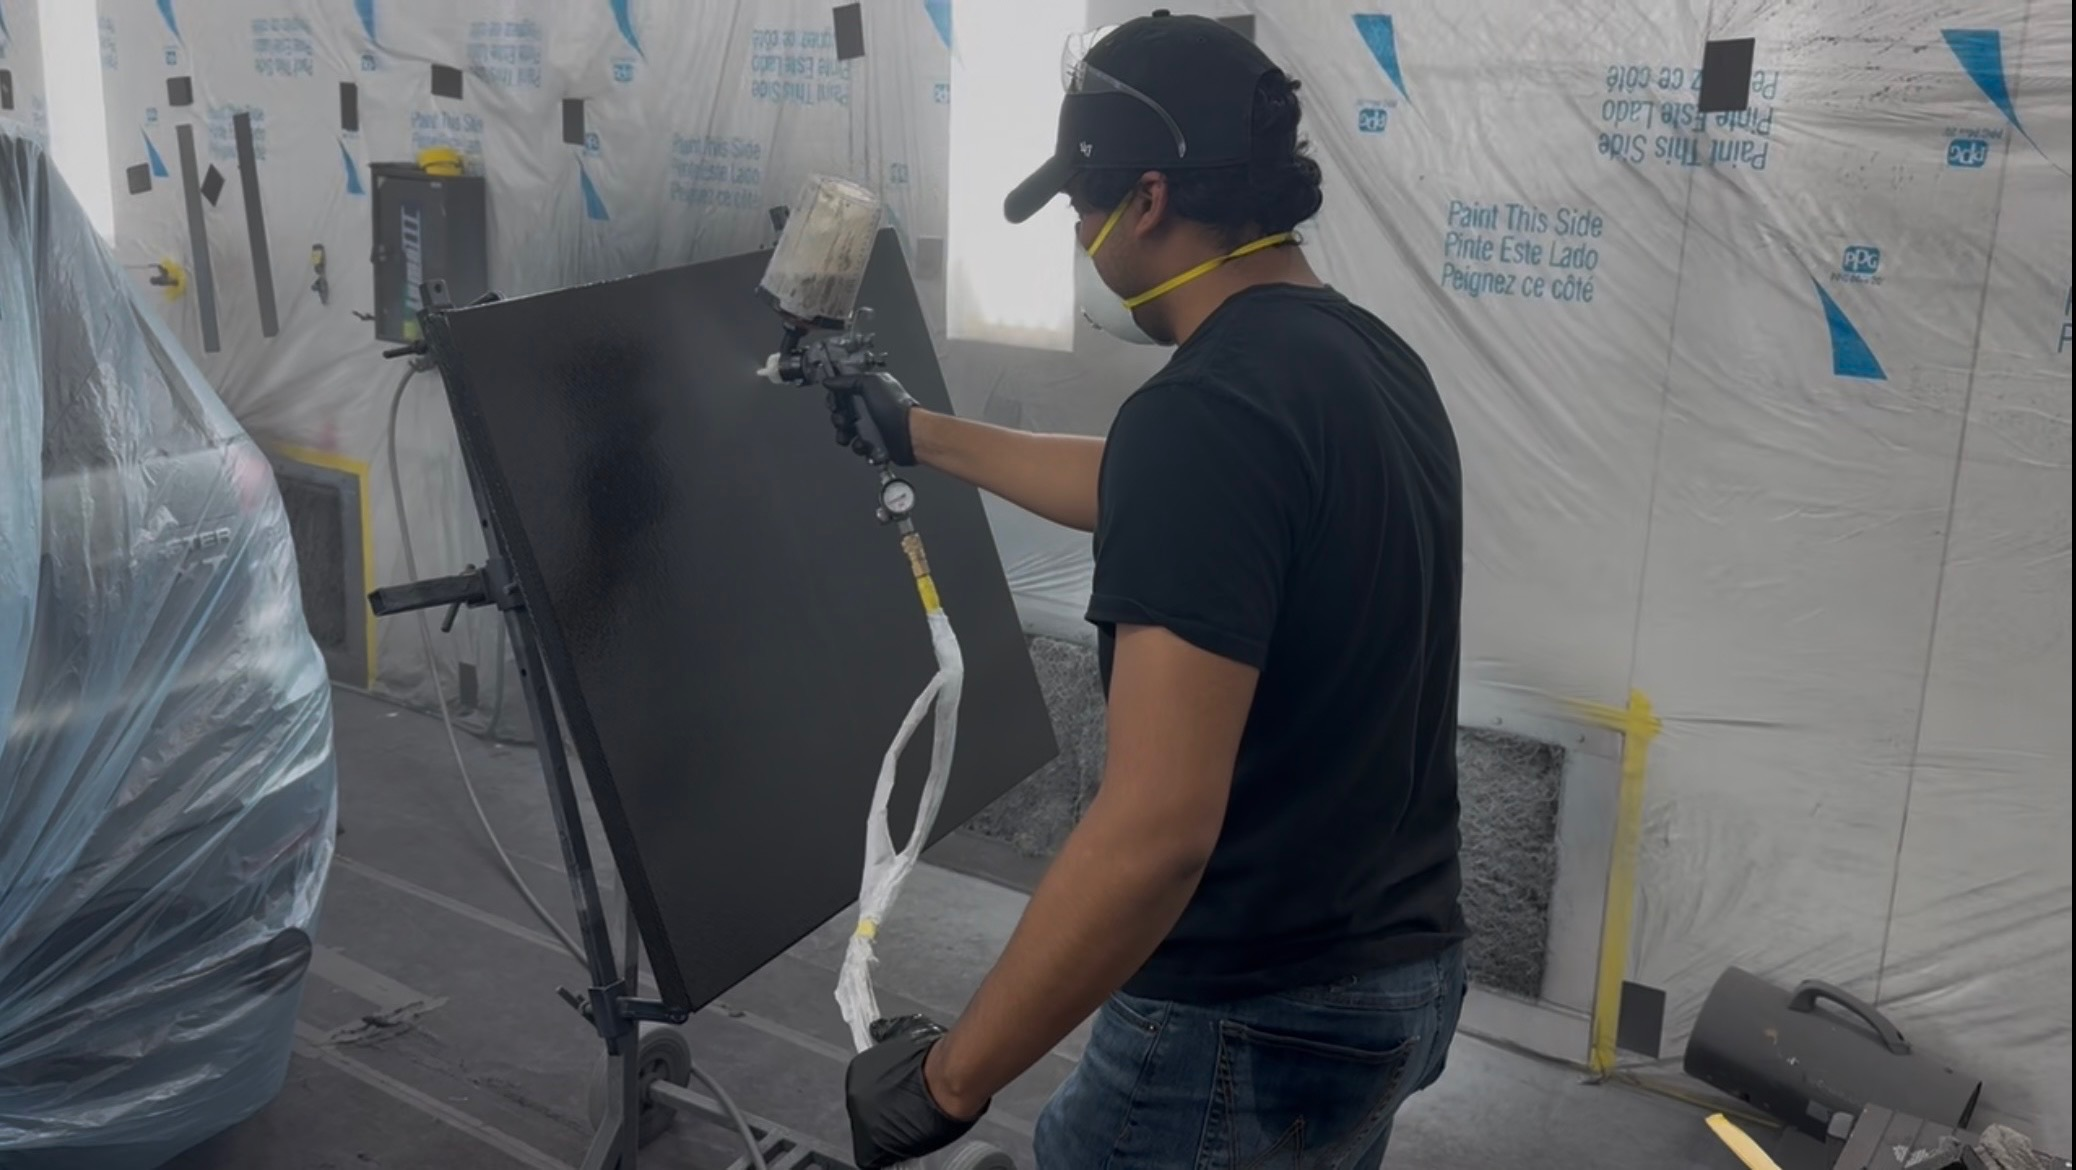
\includegraphics[
        width=2.35in,
        height=1.40in,
        keepaspectratio
    ]{spraying_topcoat}
};
\draw[RuleGray,line width=0.55pt,rounded corners=4pt]
    ($(current page.north west)+(3.10in,-1.91in)$)
    rectangle
    ($(current page.north west)+(5.65in,-3.40in)$);

% Image 3
\node[anchor=center,inner sep=0pt]
at ($(current page.north west)+(7.045in,-2.655in)$)
{
    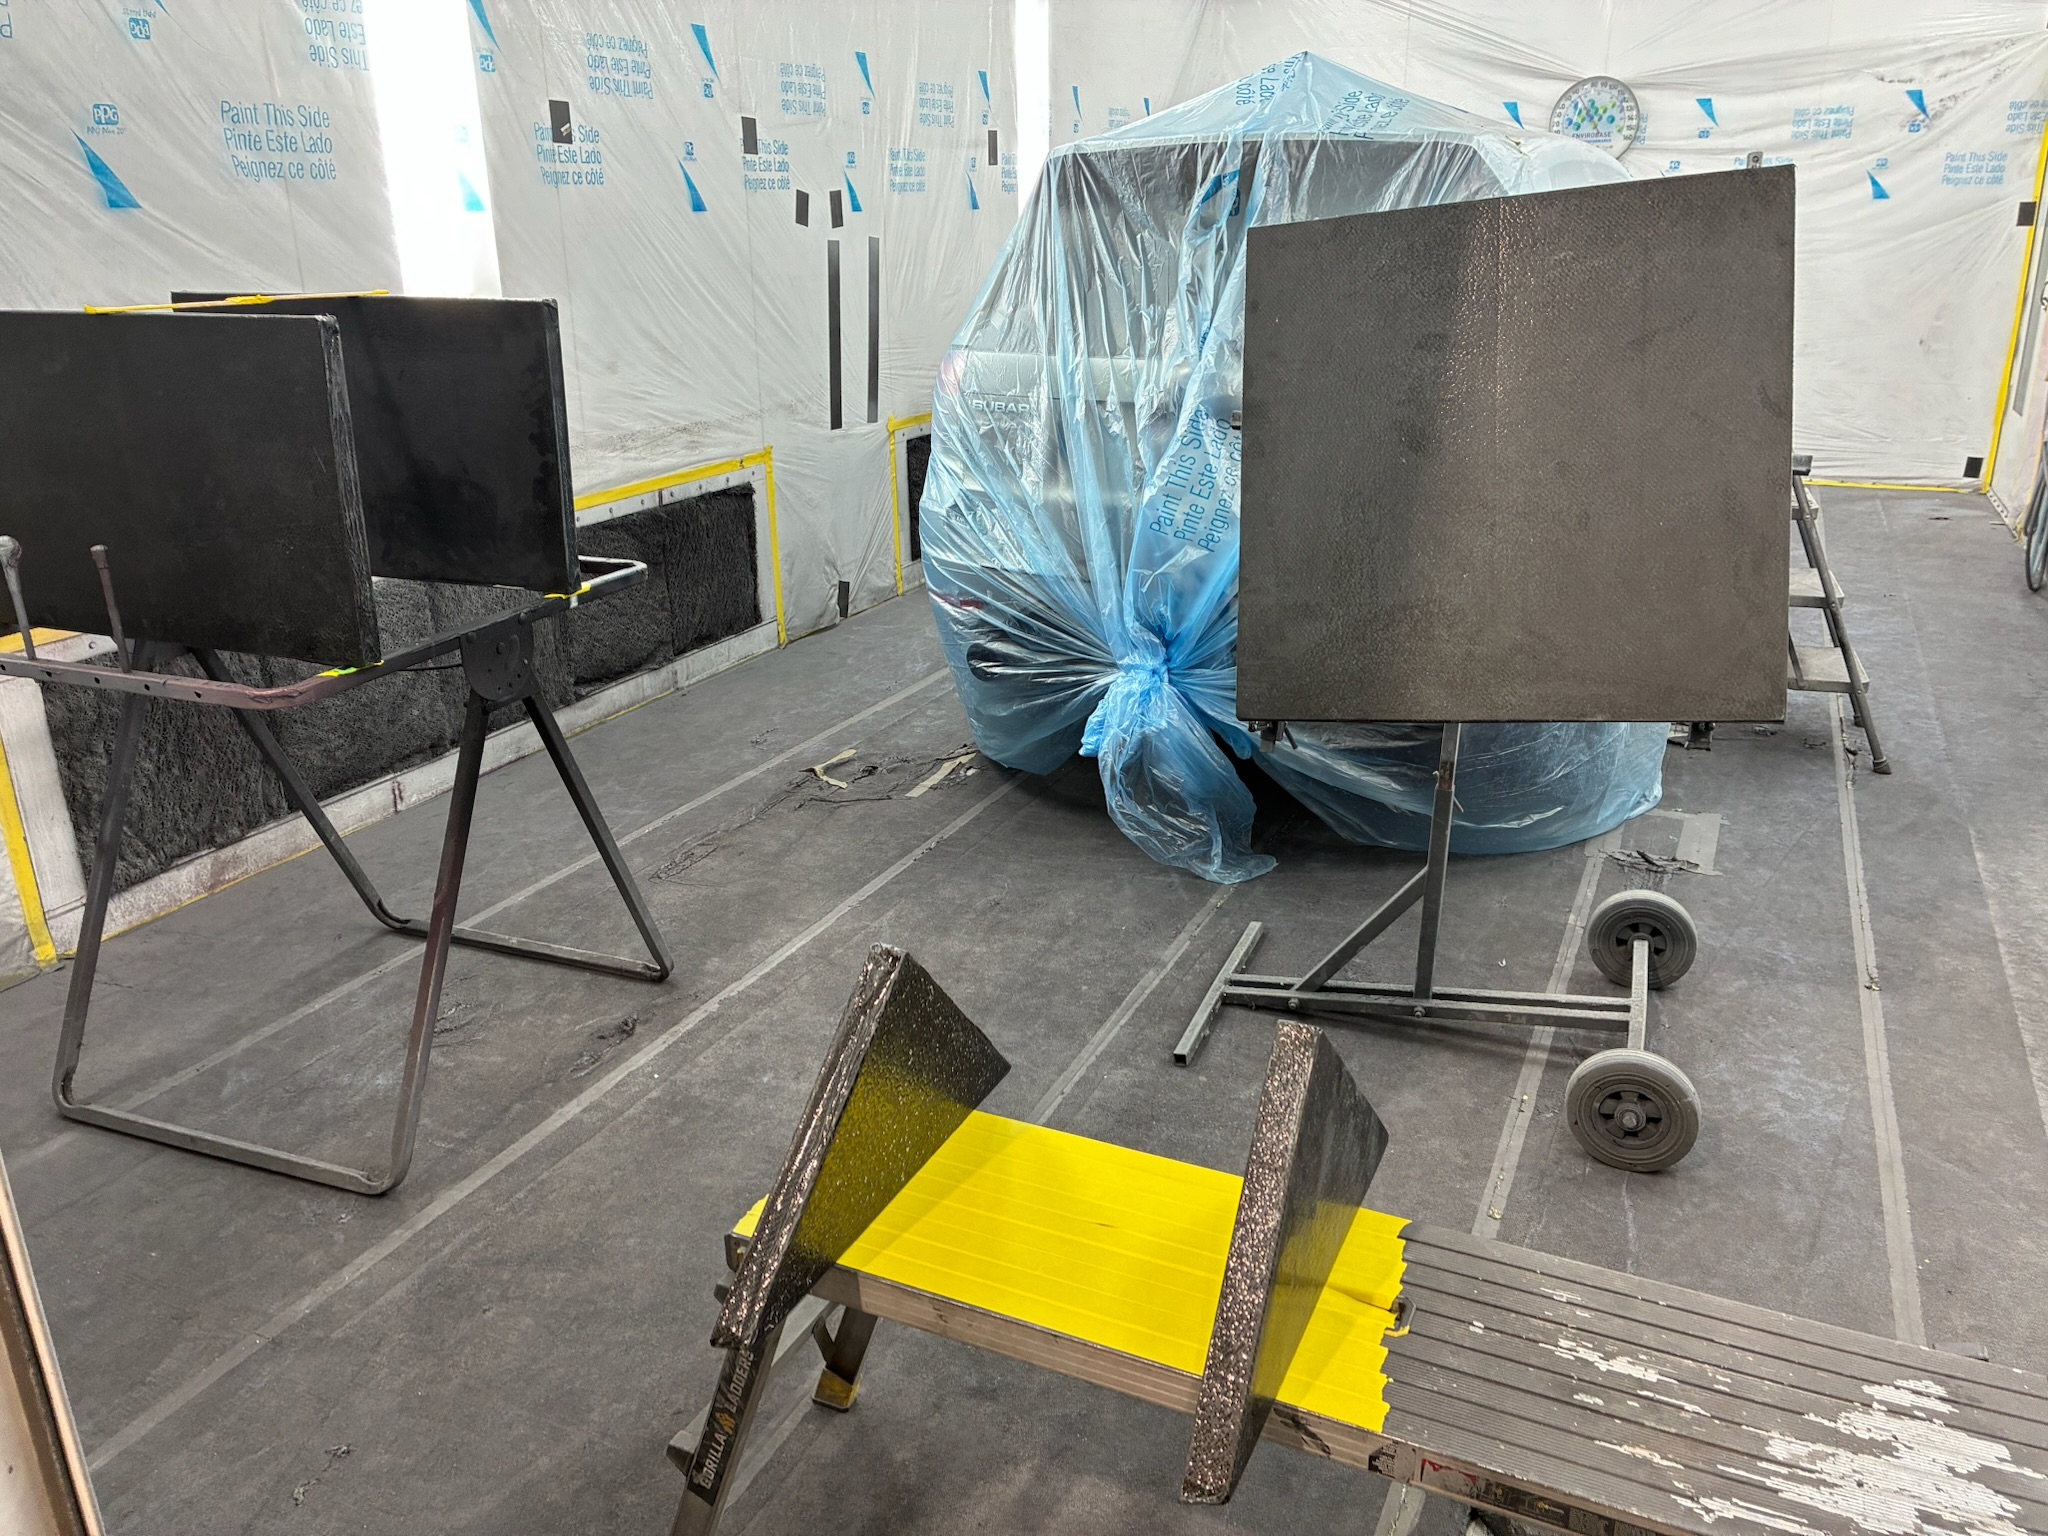
\includegraphics[
        width=2.35in,
        height=1.40in,
        keepaspectratio
    ]{topcoat_setup_apparatus}
};
\draw[RuleGray,line width=0.55pt,rounded corners=4pt]
    ($(current page.north west)+(5.77in,-1.91in)$)
    rectangle
    ($(current page.north west)+(8.32in,-3.40in)$);

% Image 4
\node[anchor=center,inner sep=0pt]
at ($(current page.north west)+(9.50in,-2.655in)$)
{
    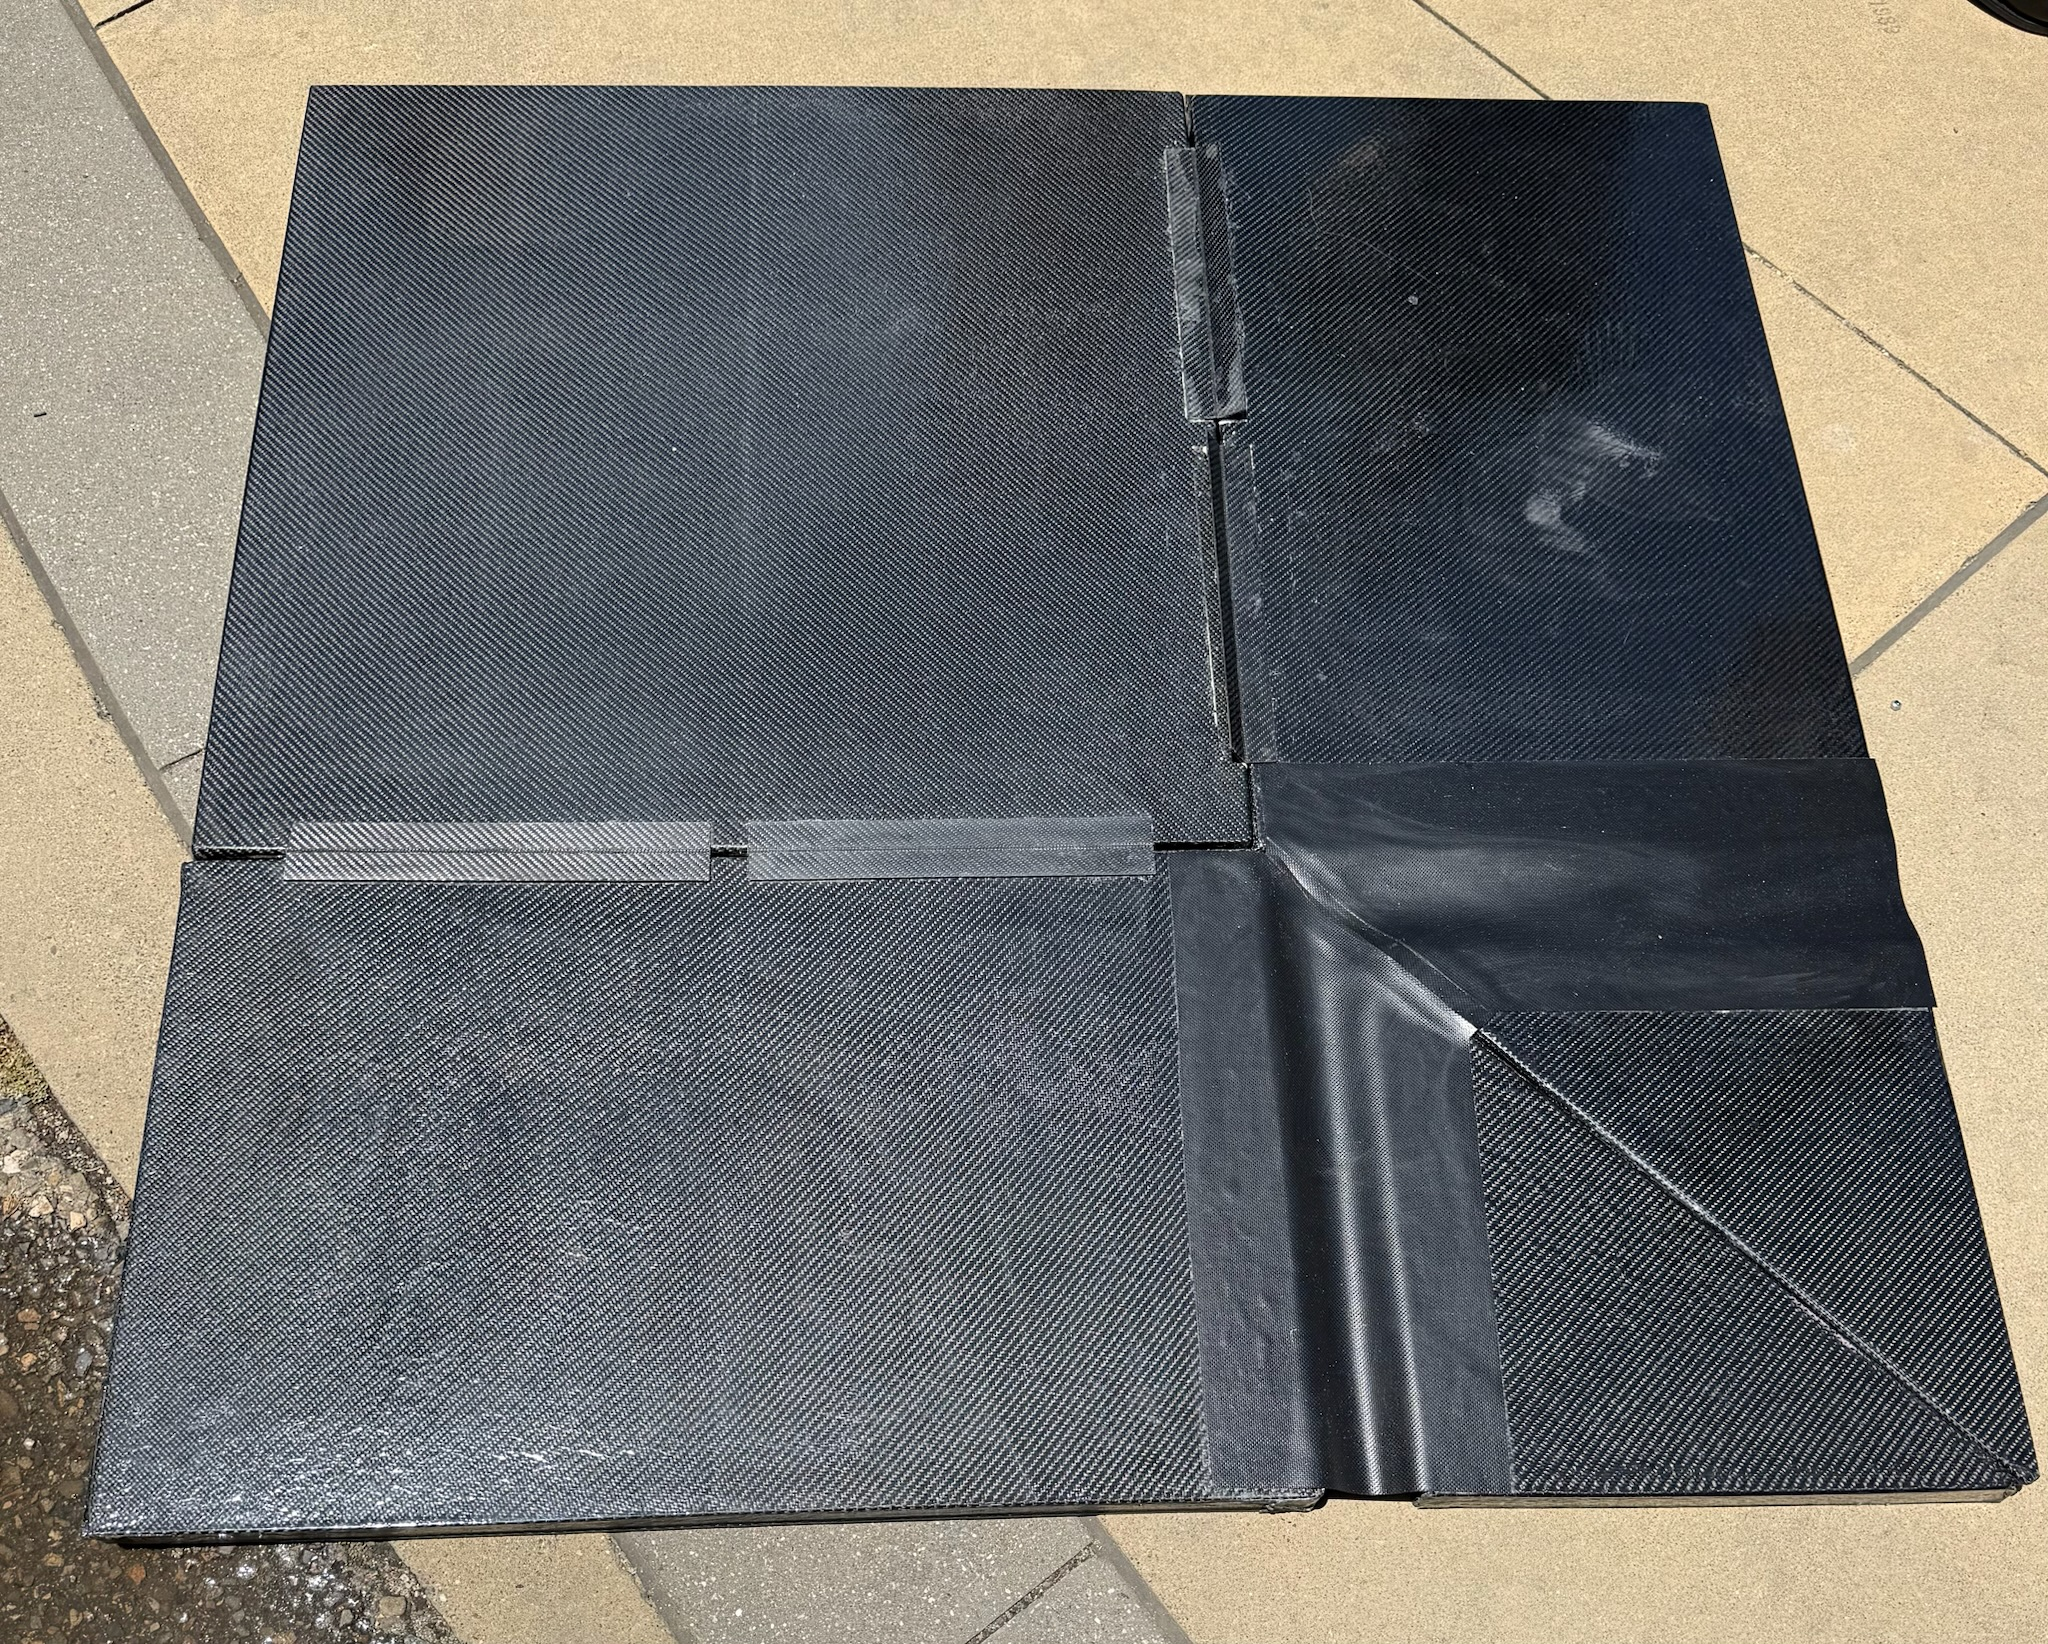
\includegraphics[
        width=2.35in,
        height=1.40in,
        keepaspectratio
    ]{refined_final_toro_cover_partial_carbon_model}
};
\draw[RuleGray,line width=0.55pt,rounded corners=4pt]
    ($(current page.north west)+(8.44in,-1.91in)$)
    rectangle
    ($(current page.north east)+(-0.42in,-3.40in)$);

% Captions
\node[anchor=north,text=Muted,font=\sffamily\fontsize{6.7}{7.3}\selectfont]
at ($(current page.north west)+(1.705in,-3.45in)$)
{Topcoat material preparation};

\node[anchor=north,text=Muted,font=\sffamily\fontsize{6.7}{7.3}\selectfont]
at ($(current page.north west)+(4.375in,-3.45in)$)
{Automotive-booth topcoat application};

\node[anchor=north,text=Muted,font=\sffamily\fontsize{6.7}{7.3}\selectfont]
at ($(current page.north west)+(7.045in,-3.45in)$)
{Coated panels drying after application};

\node[anchor=north,text=Muted,font=\sffamily\fontsize{6.7}{7.3}\selectfont]
at ($(current page.north west)+(9.50in,-3.45in)$)
{Partial carbon manufacturing model};

% Environmental rationale
\fill[SoftGold,rounded corners=4pt]
    ($(current page.north west)+(0.43in,-3.73in)$)
    rectangle
    ($(current page.north east)+(-0.42in,-4.76in)$);

\node[
    anchor=north west,
    align=left,
    text width=9.75in,
    text=Ink,
    font=\fontsize{7.05}{8.25}\selectfont
]
at ($(current page.north west)+(0.65in,-3.89in)$)
{
Because the sponsor required a carbon-fiber cover for outdoor use near chlorinated water,
environmental protection became a functional requirement rather than a cosmetic finish.
I selected and personally sprayed a UV-resistant Sunshield topcoat to seal minor laminate
porosity, reduce moisture ingress, preserve the carbon appearance, limit UV degradation of
the epoxy matrix, and isolate the composite surface from nearby metallic hardware.
};

% Results title
\node[
    anchor=north west,
    text=DeepGreen,
    font=\sffamily\bfseries\fontsize{8.0}{8.7}\selectfont
]
at ($(current page.north west)+(0.43in,-4.94in)$)
{FUNCTIONAL PROTOTYPE RESULTS};

% ------------------------------------------------------------
% Matched lower panels — larger type and improved allocation
% ------------------------------------------------------------

% Left results panel
\fill[SoftGreen,rounded corners=5pt]
    ($(current page.north west)+(0.43in,-5.22in)$)
    rectangle
    ($(current page.north west)+(5.98in,-7.39in)$);

\draw[RuleGray,line width=0.65pt,rounded corners=5pt]
    ($(current page.north west)+(0.43in,-5.22in)$)
    rectangle
    ($(current page.north west)+(5.98in,-7.39in)$);

\fill[DeepGreen,rounded corners=5pt]
    ($(current page.north west)+(0.43in,-5.22in)$)
    rectangle
    ($(current page.north west)+(5.98in,-5.58in)$);

\fill[DeepGreen]
    ($(current page.north west)+(0.43in,-5.40in)$)
    rectangle
    ($(current page.north west)+(5.98in,-5.58in)$);

\node[anchor=west,text=white,
      font=\sffamily\bfseries\fontsize{7.0}{7.6}\selectfont]
at ($(current page.north west)+(0.66in,-5.40in)$)
{SPECIFICATION};

\node[anchor=west,text=white,
      font=\sffamily\bfseries\fontsize{7.0}{7.6}\selectfont]
at ($(current page.north west)+(3.02in,-5.40in)$)
{RESULT};

\node[anchor=east,text=white,
      font=\sffamily\bfseries\fontsize{7.0}{7.6}\selectfont]
at ($(current page.north west)+(5.55in,-5.40in)$)
{STATUS};

\node[
    anchor=north west,
    align=left,
    text width=2.15in,
    text=Ink,
    font=\bfseries\fontsize{7.15}{8.55}\selectfont
]
at ($(current page.north west)+(0.66in,-5.72in)$)
{
Deployment time\\[3.4pt]
Removal time\\[3.4pt]
Single-user operation\\[3.4pt]
Single-side operation\\[3.4pt]
Deployment steps\\[3.4pt]
Removal steps\\[3.4pt]
Weight\\[3.4pt]
Folded storage
};

\node[
    anchor=north west,
    align=left,
    text width=1.45in,
    text=Ink,
    font=\fontsize{7.15}{8.55}\selectfont
]
at ($(current page.north west)+(3.02in,-5.72in)$)
{
25.51 seconds\\[3.4pt]
37.22 seconds\\[3.4pt]
100\% successful\\[3.4pt]
75\% successful\\[3.4pt]
6.4 average\\[3.4pt]
9 average\\[3.4pt]
17 lb\\[3.4pt]
2.9' x 2.9' x 1.7'
};

\node[
    anchor=north east,
    align=right,
    text width=1.05in,
    text=DeepGreen,
    font=\sffamily\bfseries\fontsize{7.05}{8.55}\selectfont
]
at ($(current page.north west)+(5.55in,-5.72in)$)
{
PASS\\[3.4pt]
PASS\\[3.4pt]
PASS\\[3.4pt]
NEAR TARGET\\[3.4pt]
PASS\\[3.4pt]
PASS\\[3.4pt]
NEAR TARGET\\[3.4pt]
PASS
};

% Right takeaways panel — widened for easier reading
\fill[SoftGreen,rounded corners=5pt]
    ($(current page.north west)+(6.14in,-5.22in)$)
    rectangle
    ($(current page.north east)+(-0.42in,-7.39in)$);

\draw[RuleGray,line width=0.65pt,rounded corners=5pt]
    ($(current page.north west)+(6.14in,-5.22in)$)
    rectangle
    ($(current page.north east)+(-0.42in,-7.39in)$);

\fill[DeepGreen,rounded corners=5pt]
    ($(current page.north west)+(6.14in,-5.22in)$)
    rectangle
    ($(current page.north east)+(-0.42in,-5.58in)$);

\fill[DeepGreen]
    ($(current page.north west)+(6.14in,-5.40in)$)
    rectangle
    ($(current page.north east)+(-0.42in,-5.58in)$);

\node[anchor=west,text=white,
      font=\sffamily\bfseries\fontsize{7.1}{7.7}\selectfont]
at ($(current page.north west)+(6.38in,-5.40in)$)
{ENGINEERING TAKEAWAYS};

\node[
    anchor=north west,
    align=left,
    text width=4.02in,
    text=Ink,
    font=\fontsize{6.75}{7.85}\selectfont
]
at ($(current page.north west)+(6.38in,-5.72in)$)
{
\textbf{Manufacturing first.}
Composite manufacturing constraints should guide the product architecture from the beginning.\\[4.5pt]
\textbf{Prioritize deliberately.}
Competing requirements must be balanced intentionally instead of maximizing every objective.\\[4.5pt]
\textbf{Lead through the process.}
Clear procedures, calm communication, and respect for teammates' strengths were essential during fabrication.\\[4.5pt]
\textbf{Next iteration.}
Reduce weight, refine the fabric-hinge fold lines, and improve panel-edge clearance.
};

% Compact concluding pathway
\node[
    anchor=center,
    align=center,
    text=PolyGold,
    font=\sffamily\bfseries\fontsize{6.3}{6.9}\selectfont
]
at ($(current page.north)+(3.06in,-7.18in)$)
{PROTOTYPE \faArrowRight\ DESIGN REFINEMENT
\faArrowRight\ REPEATABLE MANUFACTURING
\faArrowRight\ PRODUCT};

% Validation resources
\node[
    anchor=north,
    align=center,
    text=DeepGreen,
    font=\sffamily\bfseries\fontsize{6.6}{7.2}\selectfont
]
at ($(current page.north)+(0,-7.58in)$)
{\href{\ToroDeploymentLink}{\faPlayCircle\ DEPLOYMENT}
\hspace{18pt}
\href{\ToroRemovalLink}{\faPlayCircle\ REMOVAL / FOLDING}
\hspace{18pt}
\href{\ToroPosterLink}{\faFilePdf\ EXPO POSTER}
\hspace{18pt}
\href{\ToroReportLink}{\faFilePdf\ FINAL REPORT}};

% Footer
\node[
    anchor=south west,
    text=white,
    font=\sffamily\bfseries\fontsize{7.1}{7.7}\selectfont
]
at ($(current page.south west)+(0.42in,0.17in)$)
{\faArrowLeft\ MANUFACTURING-DRIVEN DESIGN};

\node[
    anchor=south,
    text=white,
    font=\sffamily\fontsize{7.0}{7.6}\selectfont
]
at ($(current page.south)+(0,0.17in)$)
{TORO COVER \hspace{6pt} 3 / 3};

\node[
    anchor=south east,
    text=white,
    font=\sffamily\bfseries\fontsize{7.1}{7.7}\selectfont
]
at ($(current page.south east)+(-0.42in,0.17in)$)
{NEXT PROJECT \faArrowRight};

\end{tikzpicture}
\input{paddle}
\clearpage
.
% 2. In main.tex, place 
% ============================================================
% TORO COVER — THREE-PAGE PORTFOLIO CASE STUDY
% Pages 3–5 of the complete portfolio
%
% IMPORTANT:
% 1. This file must NOT contain \documentclass, \begin{document},
%    \end{document}, or \input{toro}.
% 2. In main.tex, place \input{toro} before \end{document}.
% 3. Image references use the original Overleaf base filenames
%    without extensions.
% ============================================================



% ============================================================
% CLICKABLE PROJECT RESOURCES
% All links use the exact Google Drive resources supplied.
% ============================================================
\providecommand{\ToroDrawingLink}{https://drive.google.com/file/d/1A7-7wMnRNLuQDaTgxeuUCBsGNqyXzOGV/view?usp=sharing}
\providecommand{\ToroDimensionsLink}{https://drive.google.com/file/d/13sw3BNJvE8GdzlRffxoF2n5r9Gzxide7/view?usp=sharing}
\providecommand{\ToroProblemLink}{https://drive.google.com/file/d/1zHtl8zrb13F1yeN74ptawpfS5UM_xsuw/view?usp=drive_link}
\providecommand{\ToroReportLink}{https://drive.google.com/file/d/1ULZ-P46lFsC2x29ZfmRVIKgYnr9o8hMt/view?usp=drive_link}
\providecommand{\ToroPosterLink}{https://drive.google.com/file/d/1vKiKaJUcHQb_db-FkZnRF6EvtuM4hKyS/view?usp=drive_link}
\providecommand{\ToroDeploymentLink}{https://drive.google.com/file/d/1XJx34o80_mZPTl7xy93HtWAgtS3ThhvY/view?usp=drive_link}
\providecommand{\ToroRemovalLink}{https://drive.google.com/file/d/1O7xYeyB67NUwT-j1B1HeiCcHnZDYjk6_/view?usp=drive_link}

% ============================================================
% PAGE 1 — PROJECT OVERVIEW, OWNERSHIP, AND ARCHITECTURE
% ============================================================

\clearpage
\thispagestyle{empty}
\hypertarget{toro}{}
\null

\begin{tikzpicture}[remember picture,overlay]

% Background
\fill[white]
    (current page.south west)
    rectangle
    (current page.north east);

% Page bars
\fill[DeepGreen]
    (current page.north west)
    rectangle
    ($(current page.north east)+(0,-0.095in)$);

\fill[PolyGold]
    ($(current page.north west)+(0,-0.095in)$)
    rectangle
    ($(current page.north east)+(0,-0.14in)$);

\fill[DeepGreen]
    (current page.south west)
    rectangle
    ($(current page.south east)+(0,0.36in)$);

\fill[PolyGold]
    ($(current page.south west)+(0,0.36in)$)
    rectangle
    ($(current page.south east)+(0,0.405in)$);

% Header
\node[
    anchor=north west,
    text=PolyGold,
    font=\sffamily\bfseries\fontsize{8.1}{8.7}\selectfont
]
at ($(current page.north west)+(0.42in,-0.39in)$)
{01 COMPOSITES \hspace{5pt}/\hspace{5pt} PROJECT 01};

\node[
    anchor=north west,
    text=DeepGreen,
    font=\bfseries\fontsize{23.5}{24.5}\selectfont
]
at ($(current page.north west)+(0.40in,-0.67in)$)
{TORO CARBON FIBER SAFETY COVER};

\node[
    anchor=north west,
    text=Muted,
    font=\sffamily\fontsize{8.4}{9.2}\selectfont
]
at ($(current page.north west)+(0.42in,-1.12in)$)
{Cal Poly Composites Laboratory \hspace{7pt}\textbullet\hspace{7pt}
Team Project \hspace{7pt}\textbullet\hspace{7pt}
Fall--Spring 2026 \hspace{7pt}\textbullet\hspace{7pt}
San Luis Obispo, California};

\fill[PolyGold]
    ($(current page.north west)+(0.42in,-1.37in)$)
    rectangle
    ($(current page.north west)+(6.1in,-1.325in)$);

% Challenge text
\node[
    anchor=north west,
    text=DeepGreen,
    font=\sffamily\bfseries\fontsize{8.1}{8.8}\selectfont
]
at ($(current page.north west)+(0.43in,-1.61in)$)
{THE CHALLENGE};

\node[
    anchor=north west,
    align=left,
    text width=4.47in,
    text=Ink,
    font=\fontsize{8.05}{9.65}\selectfont
]
at ($(current page.north west)+(0.43in,-1.84in)$)
{
Develop a lightweight cover for a 6 ft by 6 ft in-ground spa
that could be deployed by one person, stored compactly,
provide insulation, resist a poolside environment, and maintain
a refined appearance. The sponsor supplied an ambitious but
intentionally broad project statement, requiring the team to
define the product architecture, priorities, manufacturing
strategy, and realistic path toward future commercialization.
};

% Role box
\fill[SoftGold,rounded corners=5pt]
    ($(current page.north west)+(0.42in,-2.88in)$)
    rectangle
    ($(current page.north west)+(4.98in,-4.58in)$);

\fill[PolyGold]
    ($(current page.north west)+(0.42in,-2.88in)$)
    rectangle
    ($(current page.north west)+(0.52in,-4.58in)$);

\node[
    anchor=north west,
    text=DeepGreen,
    font=\sffamily\bfseries\fontsize{8.1}{8.8}\selectfont
]
at ($(current page.north west)+(0.66in,-3.02in)$)
{MY ROLE — DESIGN \& MANUFACTURING LEAD};

\node[
    anchor=north west,
    align=left,
    text width=4.02in,
    text=Ink,
    font=\fontsize{7.05}{8.15}\selectfont
]
at ($(current page.north west)+(0.66in,-3.27in)$)
{
\textbullet\ Modeled every custom part and the complete assembly\\[1.5pt]
\textbullet\ Produced the engineering drawing package independently\\[1.5pt]
\textbullet\ Developed the composite-panel manufacturing process\\[1.5pt]
\textbullet\ Created all waterjet DXFs and manufacturing geometry\\[1.5pt]
\textbullet\ Trained teammates in wet layup and vacuum bagging\\[1.5pt]
\textbullet\ Presented feasibility, scope, and tradeoffs to the sponsor
};

% Large deployed foam-model image
\node[anchor=center,inner sep=0pt]
at ($(current page.north west)+(8.00in,-3.04in)$)
{
    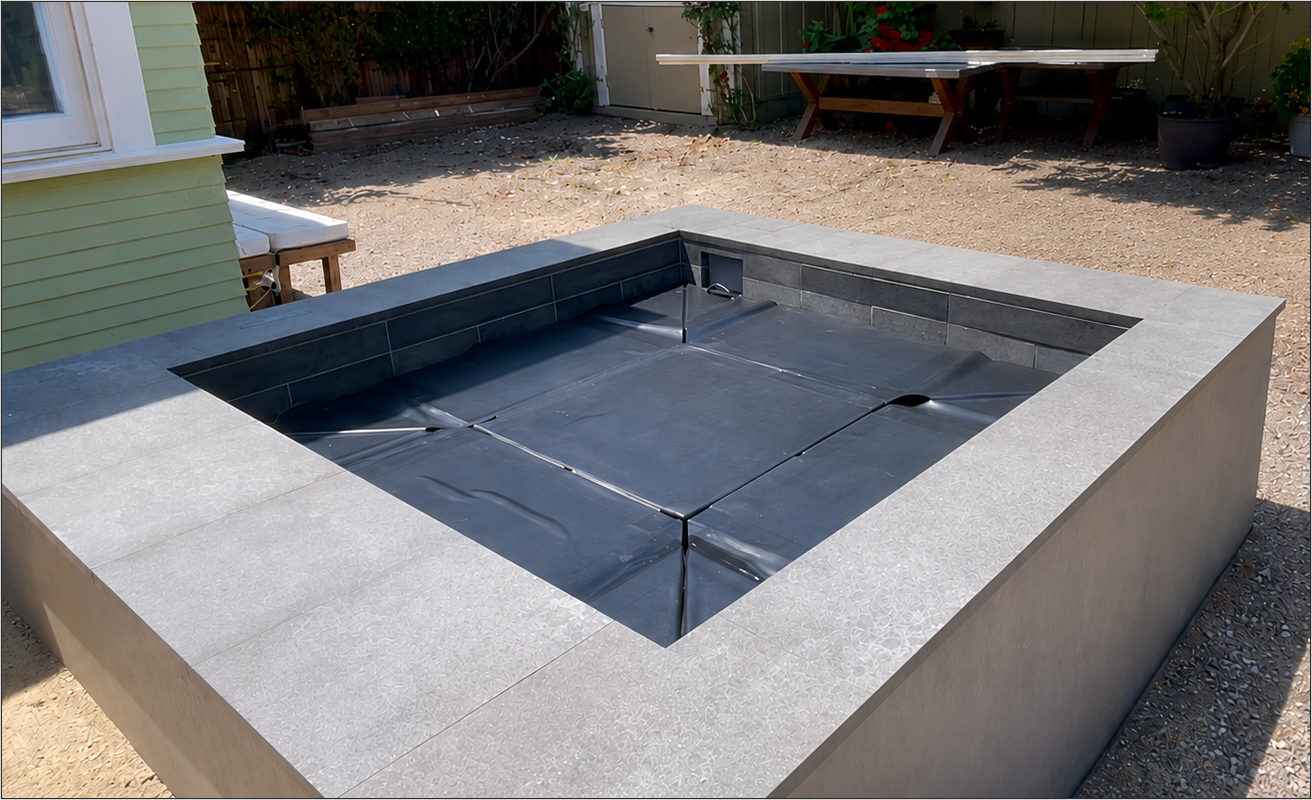
\includegraphics[
        width=5.55in,
        height=2.78in,
        keepaspectratio
    ]{deployed_functional_prototype}
};

\draw[DeepGreen,line width=0.8pt,rounded corners=7pt]
    ($(current page.north west)+(5.16in,-1.61in)$)
    rectangle
    ($(current page.north east)+(-0.42in,-4.47in)$);

\node[
    anchor=north west,
    text=Muted,
    font=\sffamily\fontsize{6.2}{6.9}\selectfont
]
at ($(current page.north west)+(5.18in,-4.54in)$)
{Functional foam model deployed over the sponsor's in-ground spa.};

% Image-strip title
\node[
    anchor=north west,
    text=DeepGreen,
    font=\sffamily\bfseries\fontsize{8.1}{8.8}\selectfont
]
at ($(current page.north west)+(0.43in,-4.78in)$)
{PRODUCT DEVELOPMENT AND FINAL ARCHITECTURE};

% Five-image development strip — CAD-first sequence
% Image 1: topside CAD
\node[anchor=center,inner sep=0pt]
at ($(current page.north west)+(1.47in,-5.73in)$)
{
    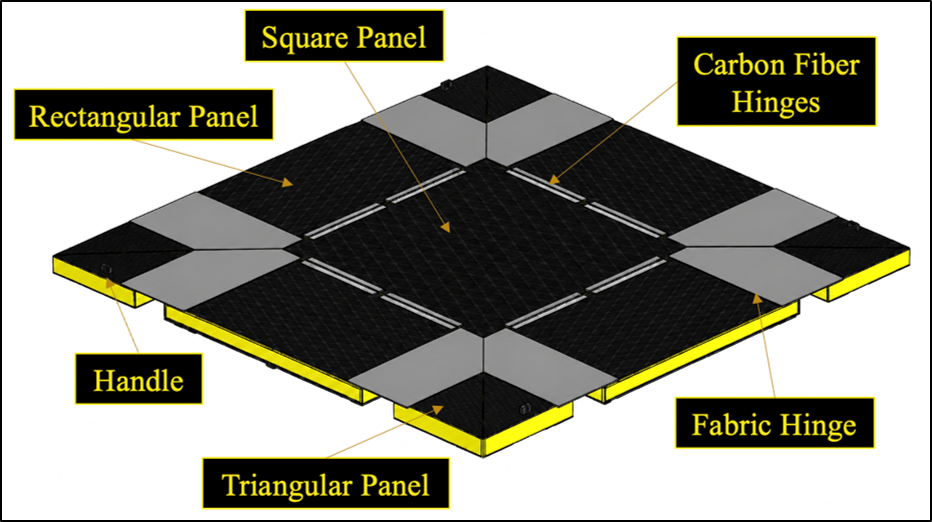
\includegraphics[
        width=1.92in,
        height=1.30in,
        keepaspectratio
    ]{Toro_Cover_topside_Cad}
};
\draw[RuleGray,line width=0.55pt,rounded corners=4pt]
    ($(current page.north west)+(0.43in,-5.04in)$)
    rectangle
    ($(current page.north west)+(2.51in,-6.43in)$);

% Image 2: underside CAD
\node[anchor=center,inner sep=0pt]
at ($(current page.north west)+(3.66in,-5.73in)$)
{
    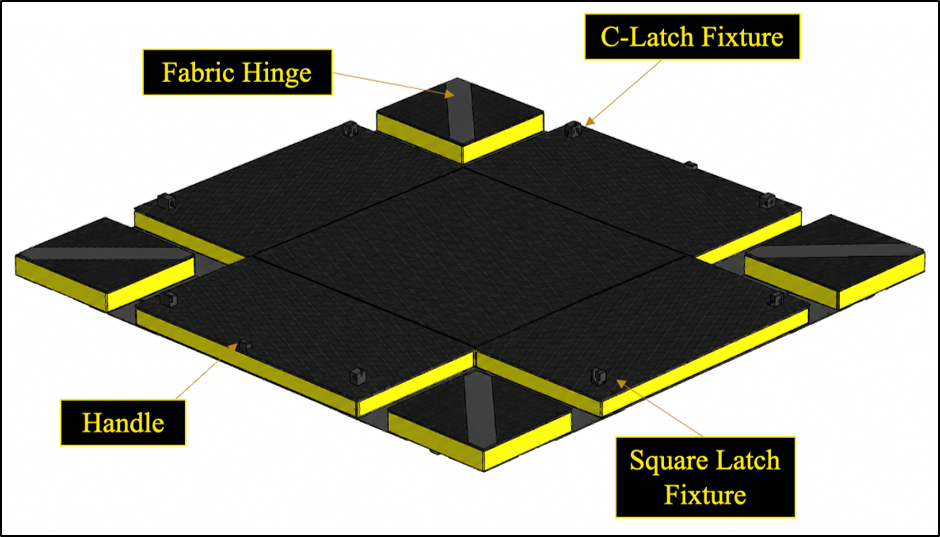
\includegraphics[
        width=1.92in,
        height=1.30in,
        keepaspectratio
    ]{toro_cover_underside_cad}
};
\draw[RuleGray,line width=0.55pt,rounded corners=4pt]
    ($(current page.north west)+(2.62in,-5.04in)$)
    rectangle
    ($(current page.north west)+(4.70in,-6.43in)$);

% Image 3: folded CAD
\node[anchor=center,inner sep=0pt]
at ($(current page.north west)+(5.85in,-5.73in)$)
{
    \includegraphics[
        width=1.92in,
        height=1.30in,
        keepaspectratio
    ]{\detokenize{Toro_Cover_folded Configuration}}
};
\draw[RuleGray,line width=0.55pt,rounded corners=4pt]
    ($(current page.north west)+(4.81in,-5.04in)$)
    rectangle
    ($(current page.north west)+(6.89in,-6.43in)$);

% Image 4: dual-use product concept
\node[anchor=center,inner sep=0pt]
at ($(current page.north west)+(8.04in,-5.73in)$)
{
    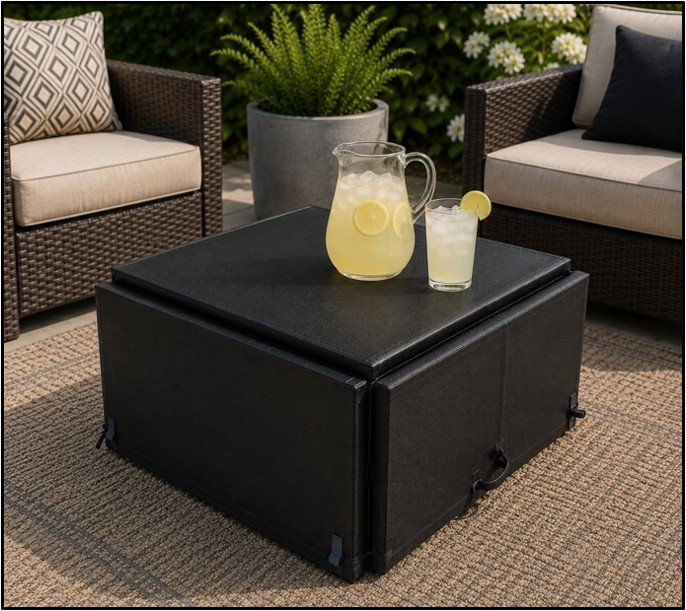
\includegraphics[
        width=1.92in,
        height=1.30in,
        keepaspectratio
    ]{generative_AI_concept_toro_cover_art}
};
\draw[RuleGray,line width=0.55pt,rounded corners=4pt]
    ($(current page.north west)+(7.00in,-5.04in)$)
    rectangle
    ($(current page.north west)+(9.08in,-6.43in)$);

% Image 5: folded foam functional prototype
% The portrait photograph is deliberately clipped to the landscape frame
% so the ottoman fills the card without extending beyond its border.
\begin{scope}
\clip[rounded corners=4pt]
    ($(current page.north west)+(9.19in,-5.04in)$)
    rectangle
    ($(current page.north east)+(-0.43in,-6.43in)$);

% Keep the original image proportions and center it within the existing card.
\node[anchor=center,inner sep=0pt]
at ($(current page.north west)+(9.88in,-5.735in)$)
{
    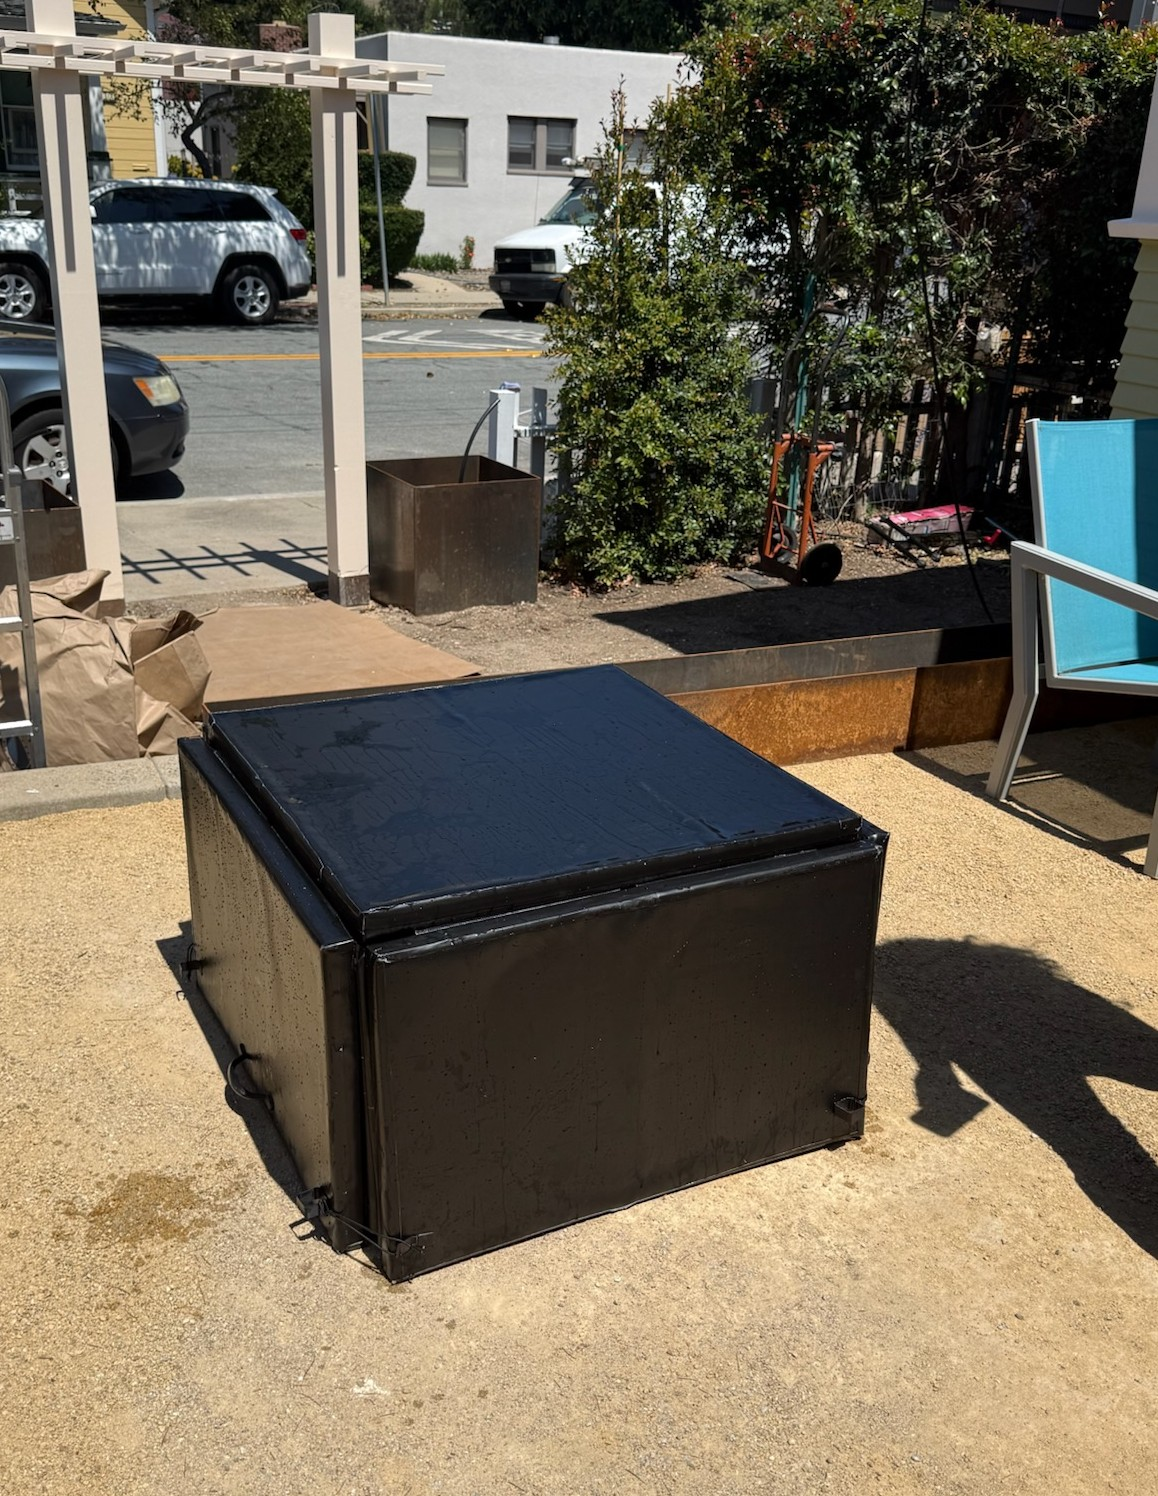
\includegraphics[
        width=1.58in,
        height=1.28in,
        keepaspectratio
    ]{foam_model_folded_backyard_image}
};
\end{scope}

\draw[RuleGray,line width=0.55pt,rounded corners=4pt]
    ($(current page.north west)+(9.19in,-5.04in)$)
    rectangle
    ($(current page.north east)+(-0.43in,-6.43in)$);

% Larger captions
\node[anchor=north,align=center,text width=1.95in,text=Muted,
      font=\sffamily\fontsize{6.8}{7.4}\selectfont]
at ($(current page.north west)+(1.47in,-6.49in)$)
{Topside panel architecture};

\node[anchor=north,align=center,text width=1.95in,text=Muted,
      font=\sffamily\fontsize{6.8}{7.4}\selectfont]
at ($(current page.north west)+(3.66in,-6.49in)$)
{Underside hinge architecture};

\node[anchor=north,align=center,text width=1.95in,text=Muted,
      font=\sffamily\fontsize{6.8}{7.4}\selectfont]
at ($(current page.north west)+(5.85in,-6.49in)$)
{Folded CAD configuration};

\node[anchor=north,align=center,text width=1.95in,text=Muted,
      font=\sffamily\fontsize{6.8}{7.4}\selectfont]
at ($(current page.north west)+(8.04in,-6.49in)$)
{Dual-use product vision};

\node[anchor=north,align=center,text width=1.95in,text=Muted,
      font=\sffamily\fontsize{6.8}{7.4}\selectfont]
at ($(current page.north west)+(9.88in,-6.49in)$)
{Folded foam prototype};

% Page 1 resource bar — centered and non-repeated resources
\fill[Panel,rounded corners=4pt]
    ($(current page.north west)+(0.43in,-7.05in)$)
    rectangle
    ($(current page.north east)+(-0.43in,-7.64in)$);
\draw[RuleGray,line width=0.5pt,rounded corners=4pt]
    ($(current page.north west)+(0.43in,-7.05in)$)
    rectangle
    ($(current page.north east)+(-0.43in,-7.64in)$);

\node[
    anchor=center,
    align=center,
    text=DeepGreen,
    font=\sffamily\bfseries\fontsize{6.9}{7.5}\selectfont
]
at ($(current page.north)+(0,-7.345in)$)
{\href{\ToroDrawingLink}{\faDraftingCompass\ DRAWING PACKAGE}
\hspace{24pt}
\href{\ToroDimensionsLink}{\faImage\ DIMENSION STUDY}
\hspace{24pt}
\href{\ToroProblemLink}{\faFileImage\ PROBLEM STATEMENT}};

% Footer
\node[
    anchor=south west,
    text=white,
    font=\sffamily\bfseries\fontsize{7.1}{7.7}\selectfont
]
at ($(current page.south west)+(0.42in,0.17in)$)
{\hyperlink{composites}{\faArrowLeft\ COMPOSITES}};

\node[
    anchor=south,
    text=white,
    font=\sffamily\fontsize{7.0}{7.6}\selectfont
]
at ($(current page.south)+(0,0.17in)$)
{TORO COVER \hspace{6pt} 1 / 3};

\node[
    anchor=south east,
    text=white,
    font=\sffamily\bfseries\fontsize{7.1}{7.7}\selectfont
]
at ($(current page.south east)+(-0.42in,0.17in)$)
{MANUFACTURING-DRIVEN DESIGN \faArrowRight};

\end{tikzpicture}


% ============================================================
% PAGE 2 — MANUFACTURING-DRIVEN DESIGN
% ============================================================

\clearpage
\thispagestyle{empty}
\hypertarget{toro-manufacturing}{}
\null

\begin{tikzpicture}[remember picture,overlay]

% Background and bars
\fill[white]
    (current page.south west)
    rectangle
    (current page.north east);

\fill[DeepGreen]
    (current page.north west)
    rectangle
    ($(current page.north east)+(0,-0.095in)$);

\fill[PolyGold]
    ($(current page.north west)+(0,-0.095in)$)
    rectangle
    ($(current page.north east)+(0,-0.14in)$);

\fill[DeepGreen]
    (current page.south west)
    rectangle
    ($(current page.south east)+(0,0.36in)$);

\fill[PolyGold]
    ($(current page.south west)+(0,0.36in)$)
    rectangle
    ($(current page.south east)+(0,0.405in)$);

% Header
\node[
    anchor=north west,
    text=PolyGold,
    font=\sffamily\bfseries\fontsize{8.1}{8.7}\selectfont
]
at ($(current page.north west)+(0.42in,-0.39in)$)
{TORO COVER \hspace{5pt}/\hspace{5pt} DESIGN FOR MANUFACTURABILITY};

\node[
    anchor=north west,
    text=DeepGreen,
    font=\bfseries\fontsize{23}{24}\selectfont
]
at ($(current page.north west)+(0.40in,-0.67in)$)
{THE ENVELOPE METHOD};

\node[
    anchor=north west,
    text=Muted,
    font=\sffamily\fontsize{8.7}{9.6}\selectfont
]
at ($(current page.north west)+(0.42in,-1.12in)$)
{A one-layup process developed for unusually thick insulated composite sandwich panels};

\fill[PolyGold]
    ($(current page.north west)+(0.42in,-1.36in)$)
    rectangle
    ($(current page.north west)+(5.30in,-1.315in)$);

% Process explanation
\fill[SoftGold,rounded corners=5pt]
    ($(current page.north west)+(0.42in,-1.61in)$)
    rectangle
    ($(current page.north east)+(-0.42in,-2.90in)$);

\fill[PolyGold]
    ($(current page.north west)+(0.42in,-1.61in)$)
    rectangle
    ($(current page.north west)+(0.52in,-2.90in)$);

\node[
    anchor=north west,
    text=DeepGreen,
    font=\sffamily\bfseries\fontsize{7.9}{8.6}\selectfont
]
at ($(current page.north west)+(0.67in,-1.76in)$)
{PROCESS INNOVATION};

\node[
    anchor=north west,
    align=left,
    text width=9.55in,
    text=Ink,
    font=\fontsize{7.35}{8.75}\selectfont
]
at ($(current page.north west)+(0.67in,-2.02in)$)
{
Weight reduction and insulation were both essential, leading to the selection of an
XPS foam core. Because XPS could not tolerate composite heat-cure temperatures, prepreg
processing was not practical and the panels had to be manufactured by wet layup with a
room-temperature cure. To simplify this process, I waterjet-cut XPS perimeter strips from
excess foam and placed them around each core inside the vacuum enclosure. Under vacuum,
the top and bottom carbon skins met along the panel sides and compressed against this
border, eliminating a separate edge-banding layup and reducing corner pleating.
};

% Workflow title
\node[
    anchor=north west,
    text=DeepGreen,
    font=\sffamily\bfseries\fontsize{8.0}{8.7}\selectfont
]
at ($(current page.north west)+(0.43in,-3.06in)$)
{MANUFACTURING WORKFLOW};

% Row 1 image 1
\node[anchor=center,inner sep=0pt]
at ($(current page.north west)+(2.07in,-4.105in)$)
{
    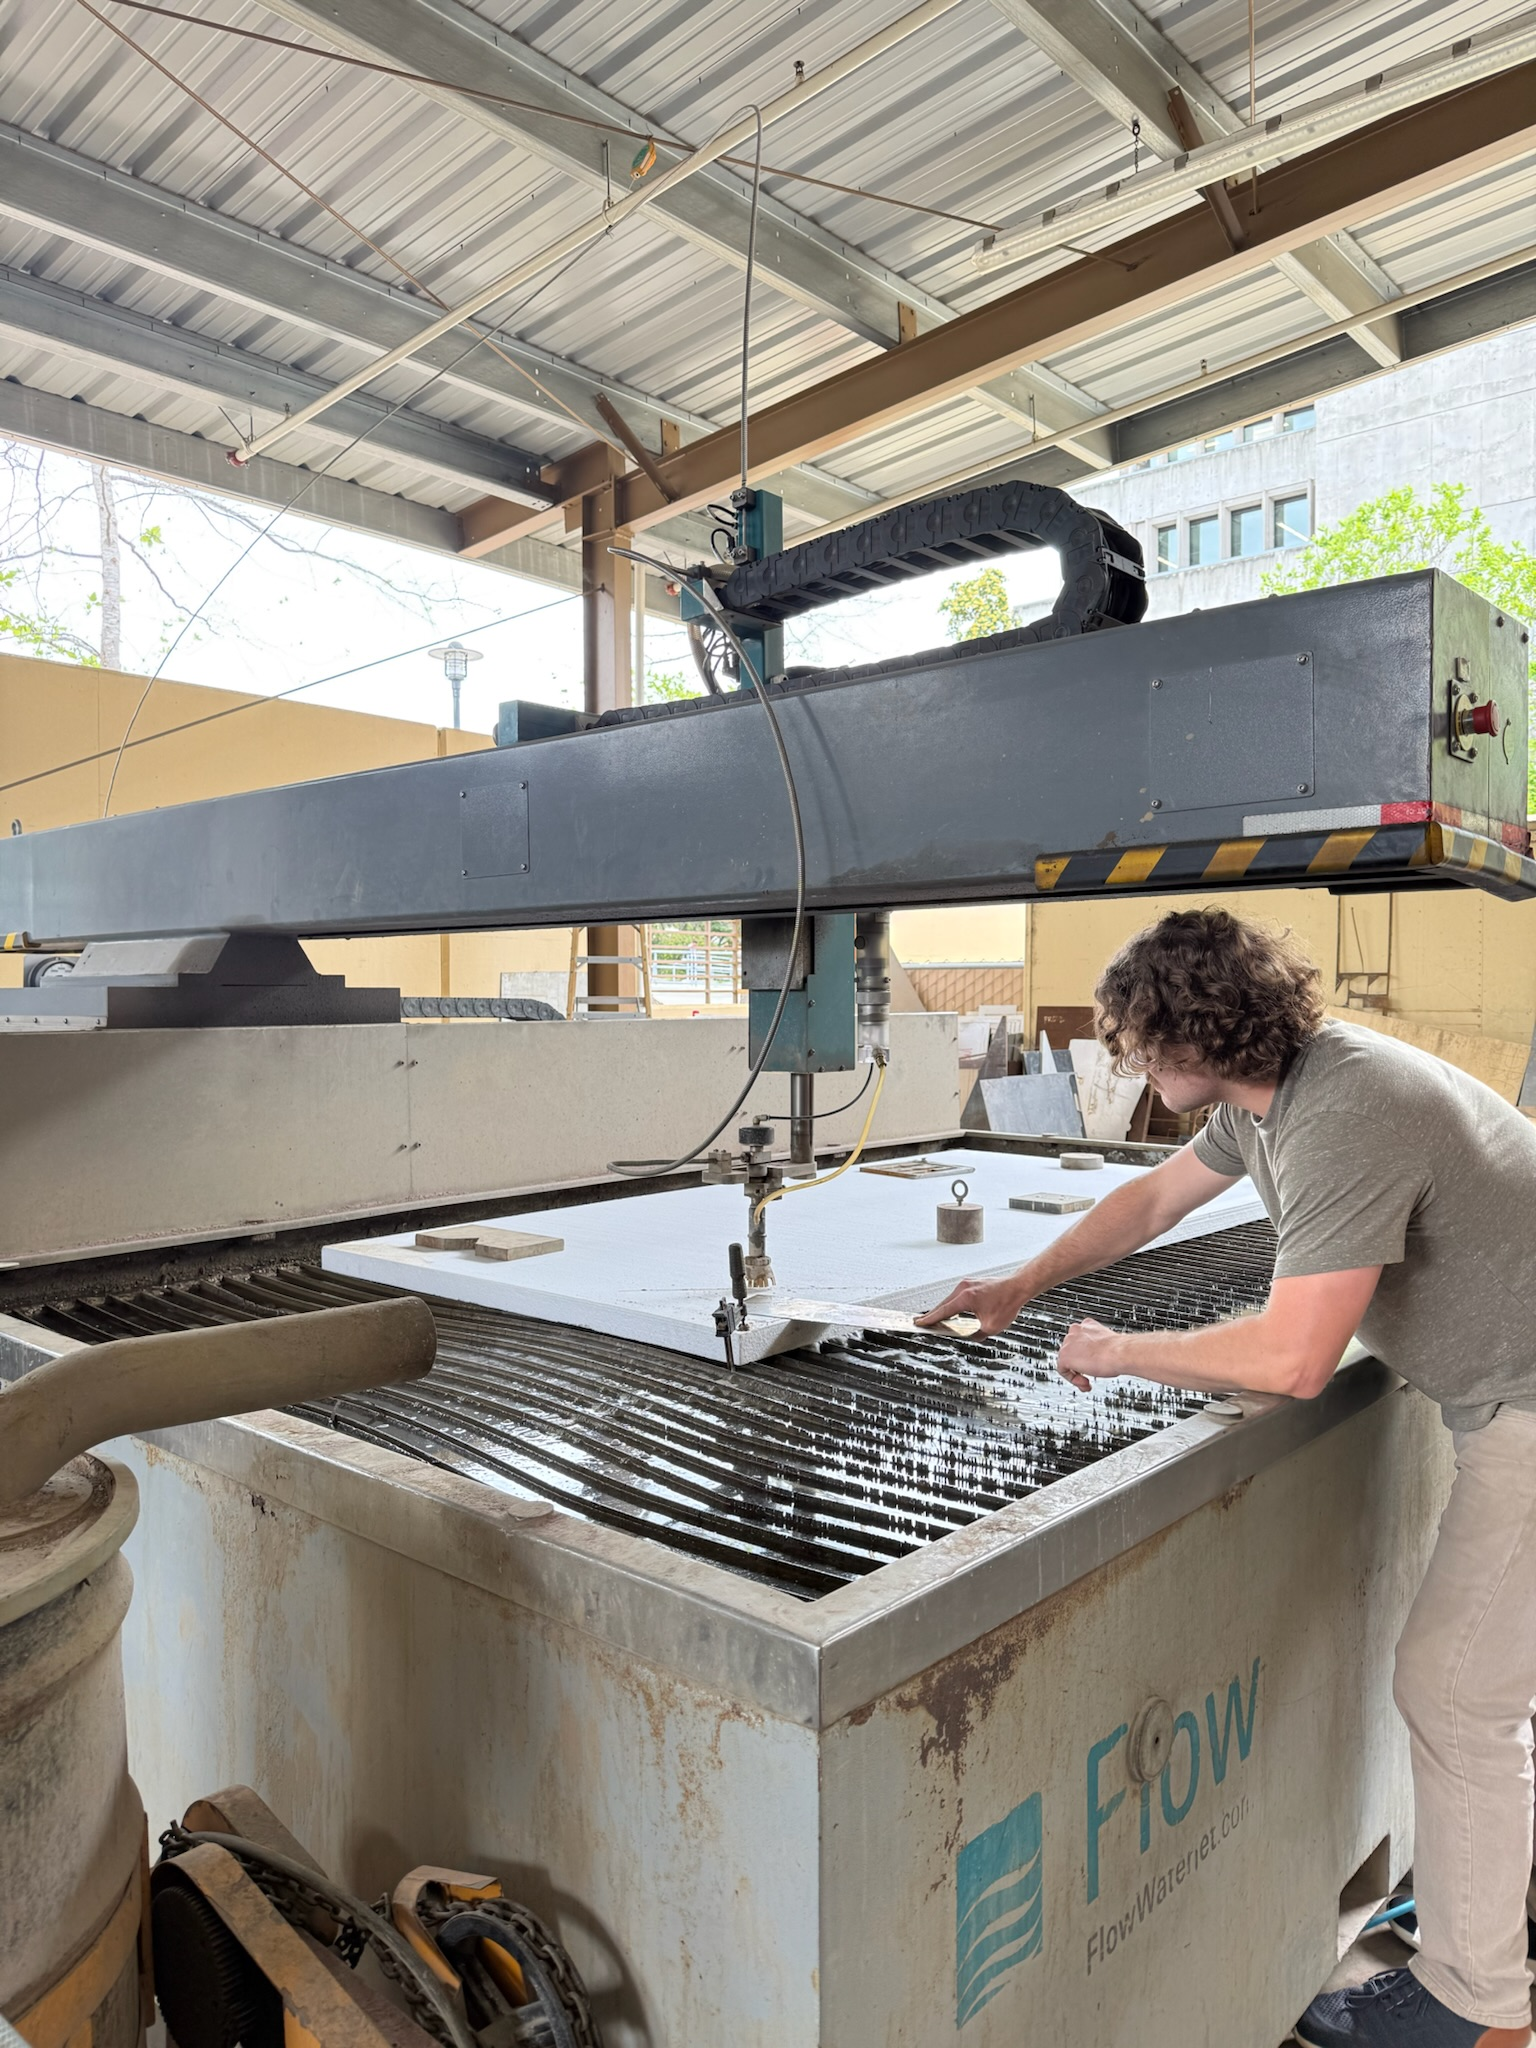
\includegraphics[
        width=3.10in,
        height=1.40in,
        keepaspectratio
    ]{waterjet_foam}
};
\draw[RuleGray,line width=0.55pt,rounded corners=4pt]
    ($(current page.north west)+(0.43in,-3.36in)$)
    rectangle
    ($(current page.north west)+(3.71in,-4.85in)$);

% Row 1 image 2
\node[anchor=center,inner sep=0pt]
at ($(current page.north west)+(5.50in,-4.105in)$)
{
    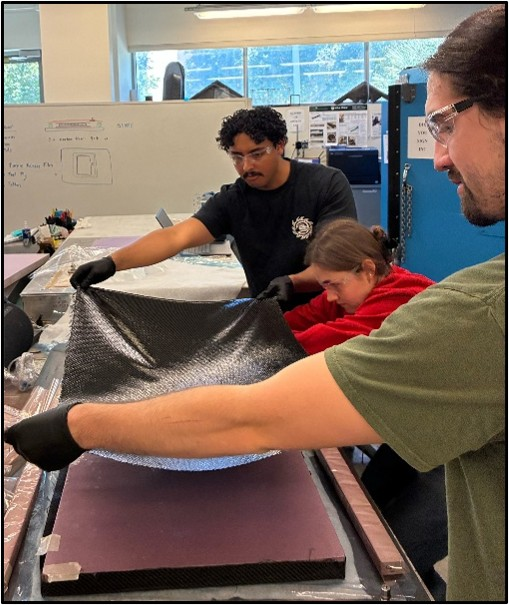
\includegraphics[
        width=3.10in,
        height=1.40in,
        keepaspectratio
    ]{group_layup}
};
\draw[RuleGray,line width=0.55pt,rounded corners=4pt]
    ($(current page.north west)+(3.86in,-3.36in)$)
    rectangle
    ($(current page.north west)+(7.14in,-4.85in)$);

% Row 1 image 3
\node[anchor=center,inner sep=0pt]
at ($(current page.north west)+(8.935in,-4.105in)$)
{
    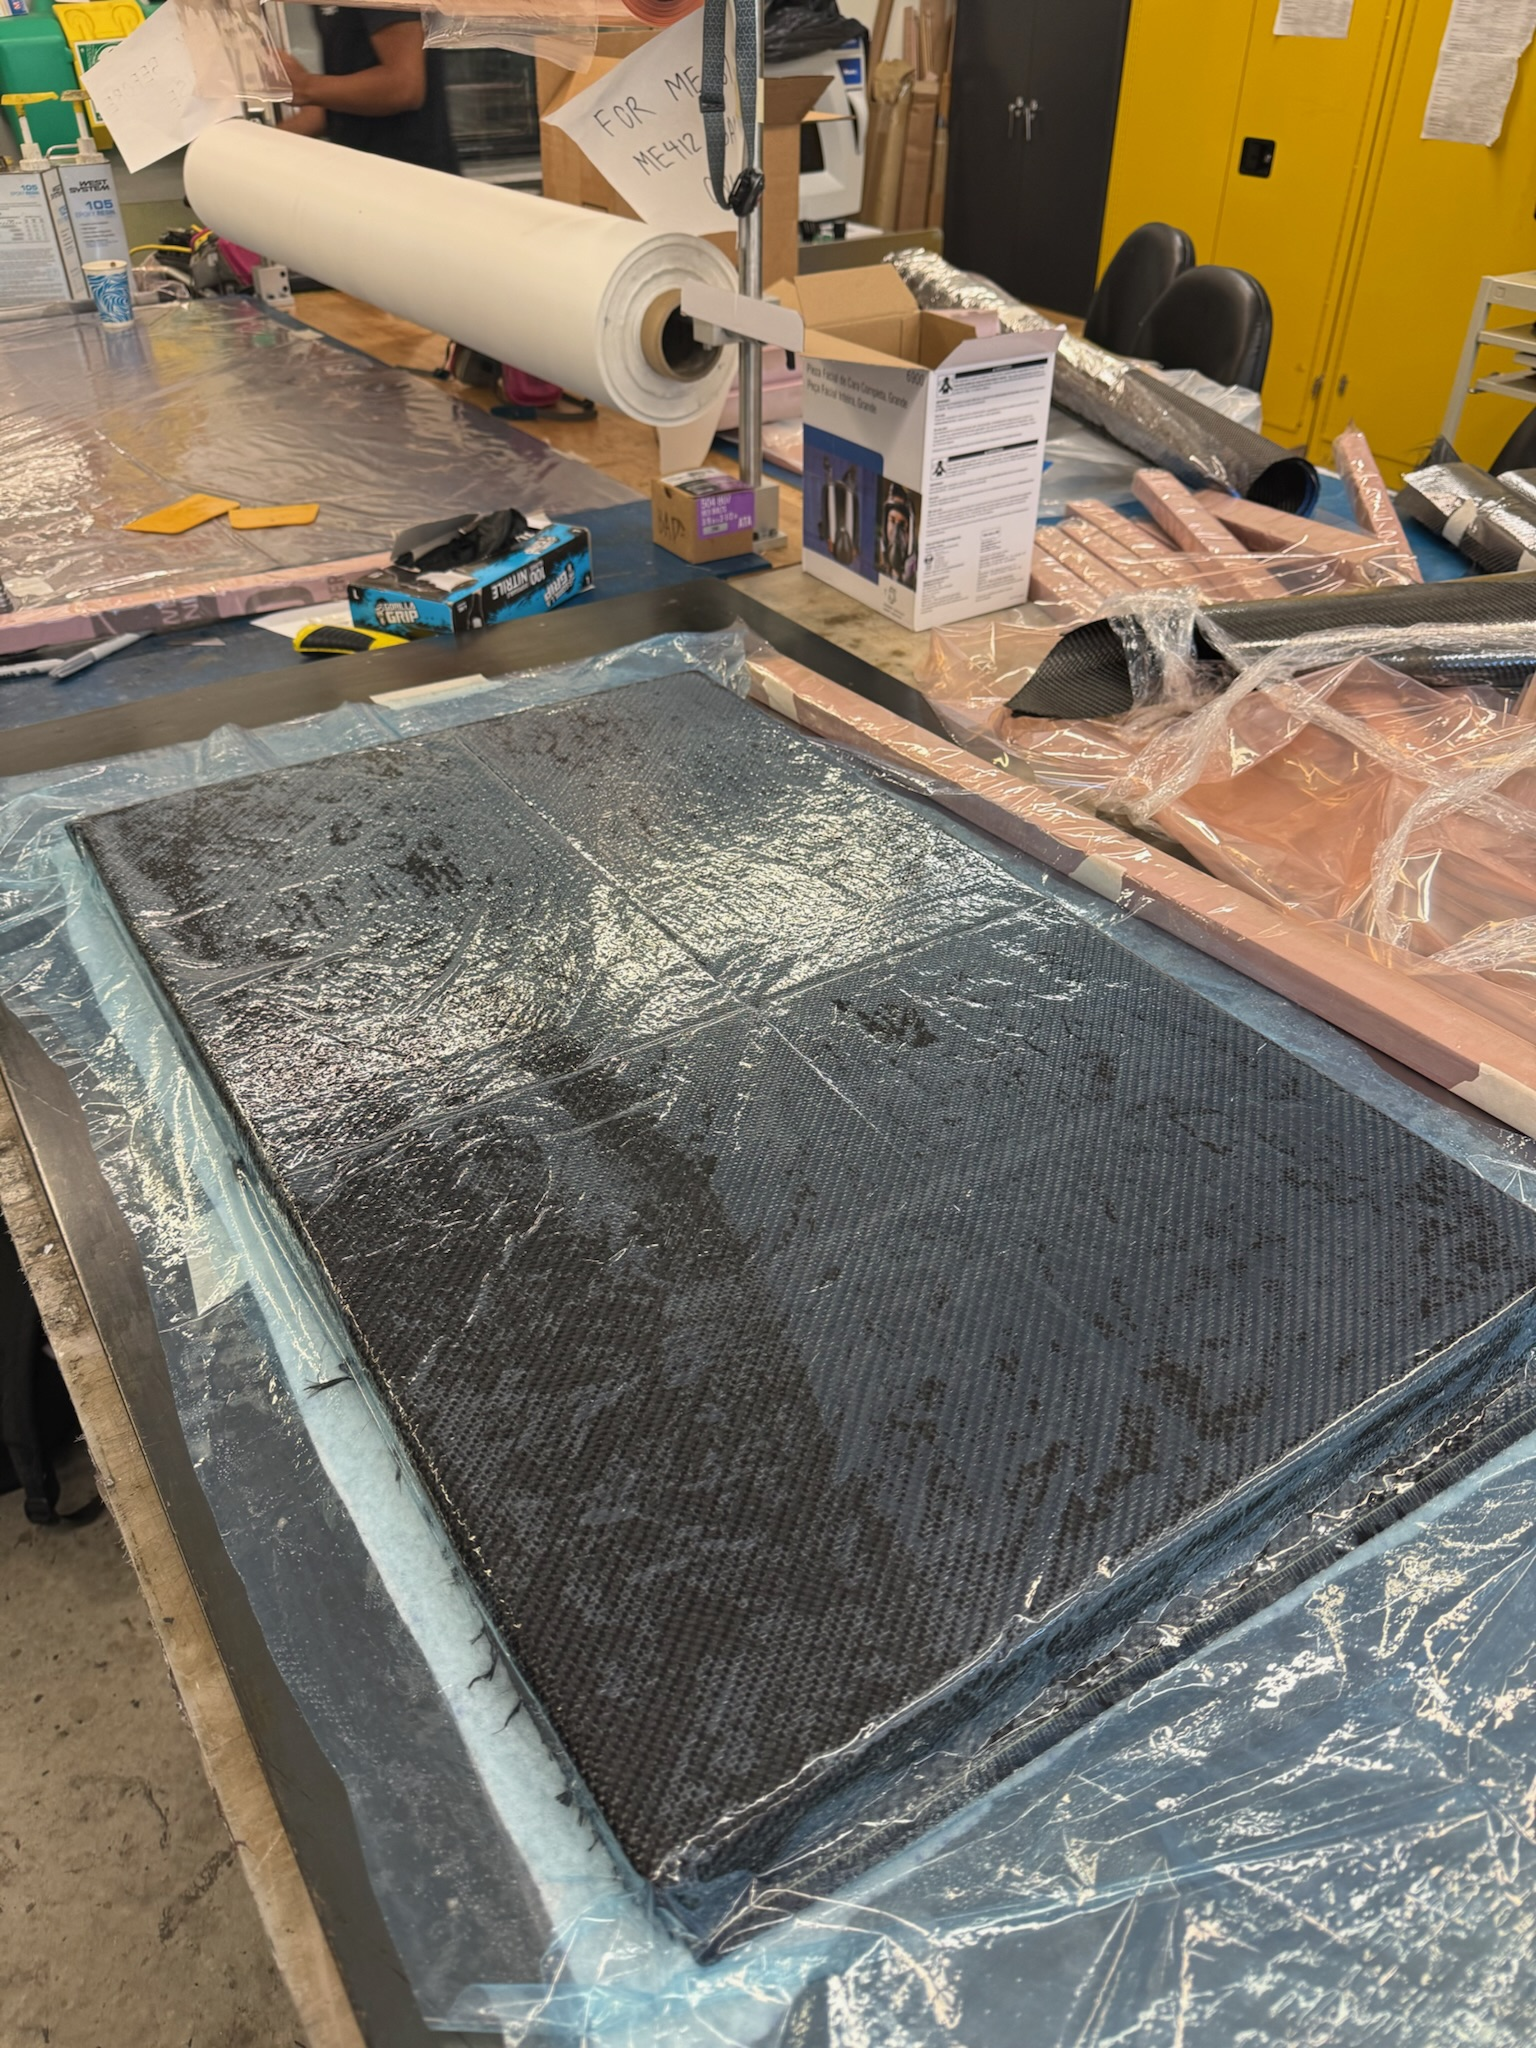
\includegraphics[
        width=3.10in,
        height=1.40in,
        keepaspectratio
    ]{blue_perforrated_film_layup}
};
\draw[RuleGray,line width=0.55pt,rounded corners=4pt]
    ($(current page.north west)+(7.29in,-3.36in)$)
    rectangle
    ($(current page.north east)+(-0.42in,-4.85in)$);

% Row 1 captions
\node[anchor=north,text=Muted,font=\sffamily\fontsize{6.7}{7.3}\selectfont]
at ($(current page.north west)+(2.07in,-4.90in)$)
{1. Waterjet-cut core and perimeter geometry};

\node[anchor=north,text=Muted,font=\sffamily\fontsize{6.7}{7.3}\selectfont]
at ($(current page.north west)+(5.50in,-4.90in)$)
{2. Team wet layup under my process guidance};

\node[anchor=north,text=Muted,font=\sffamily\fontsize{6.7}{7.3}\selectfont]
at ($(current page.north west)+(8.935in,-4.90in)$)
{3. Perforated film, breather, and vacuum enclosure};

% Row 2 image 1
\node[anchor=center,inner sep=0pt]
at ($(current page.north west)+(2.07in,-5.875in)$)
{
    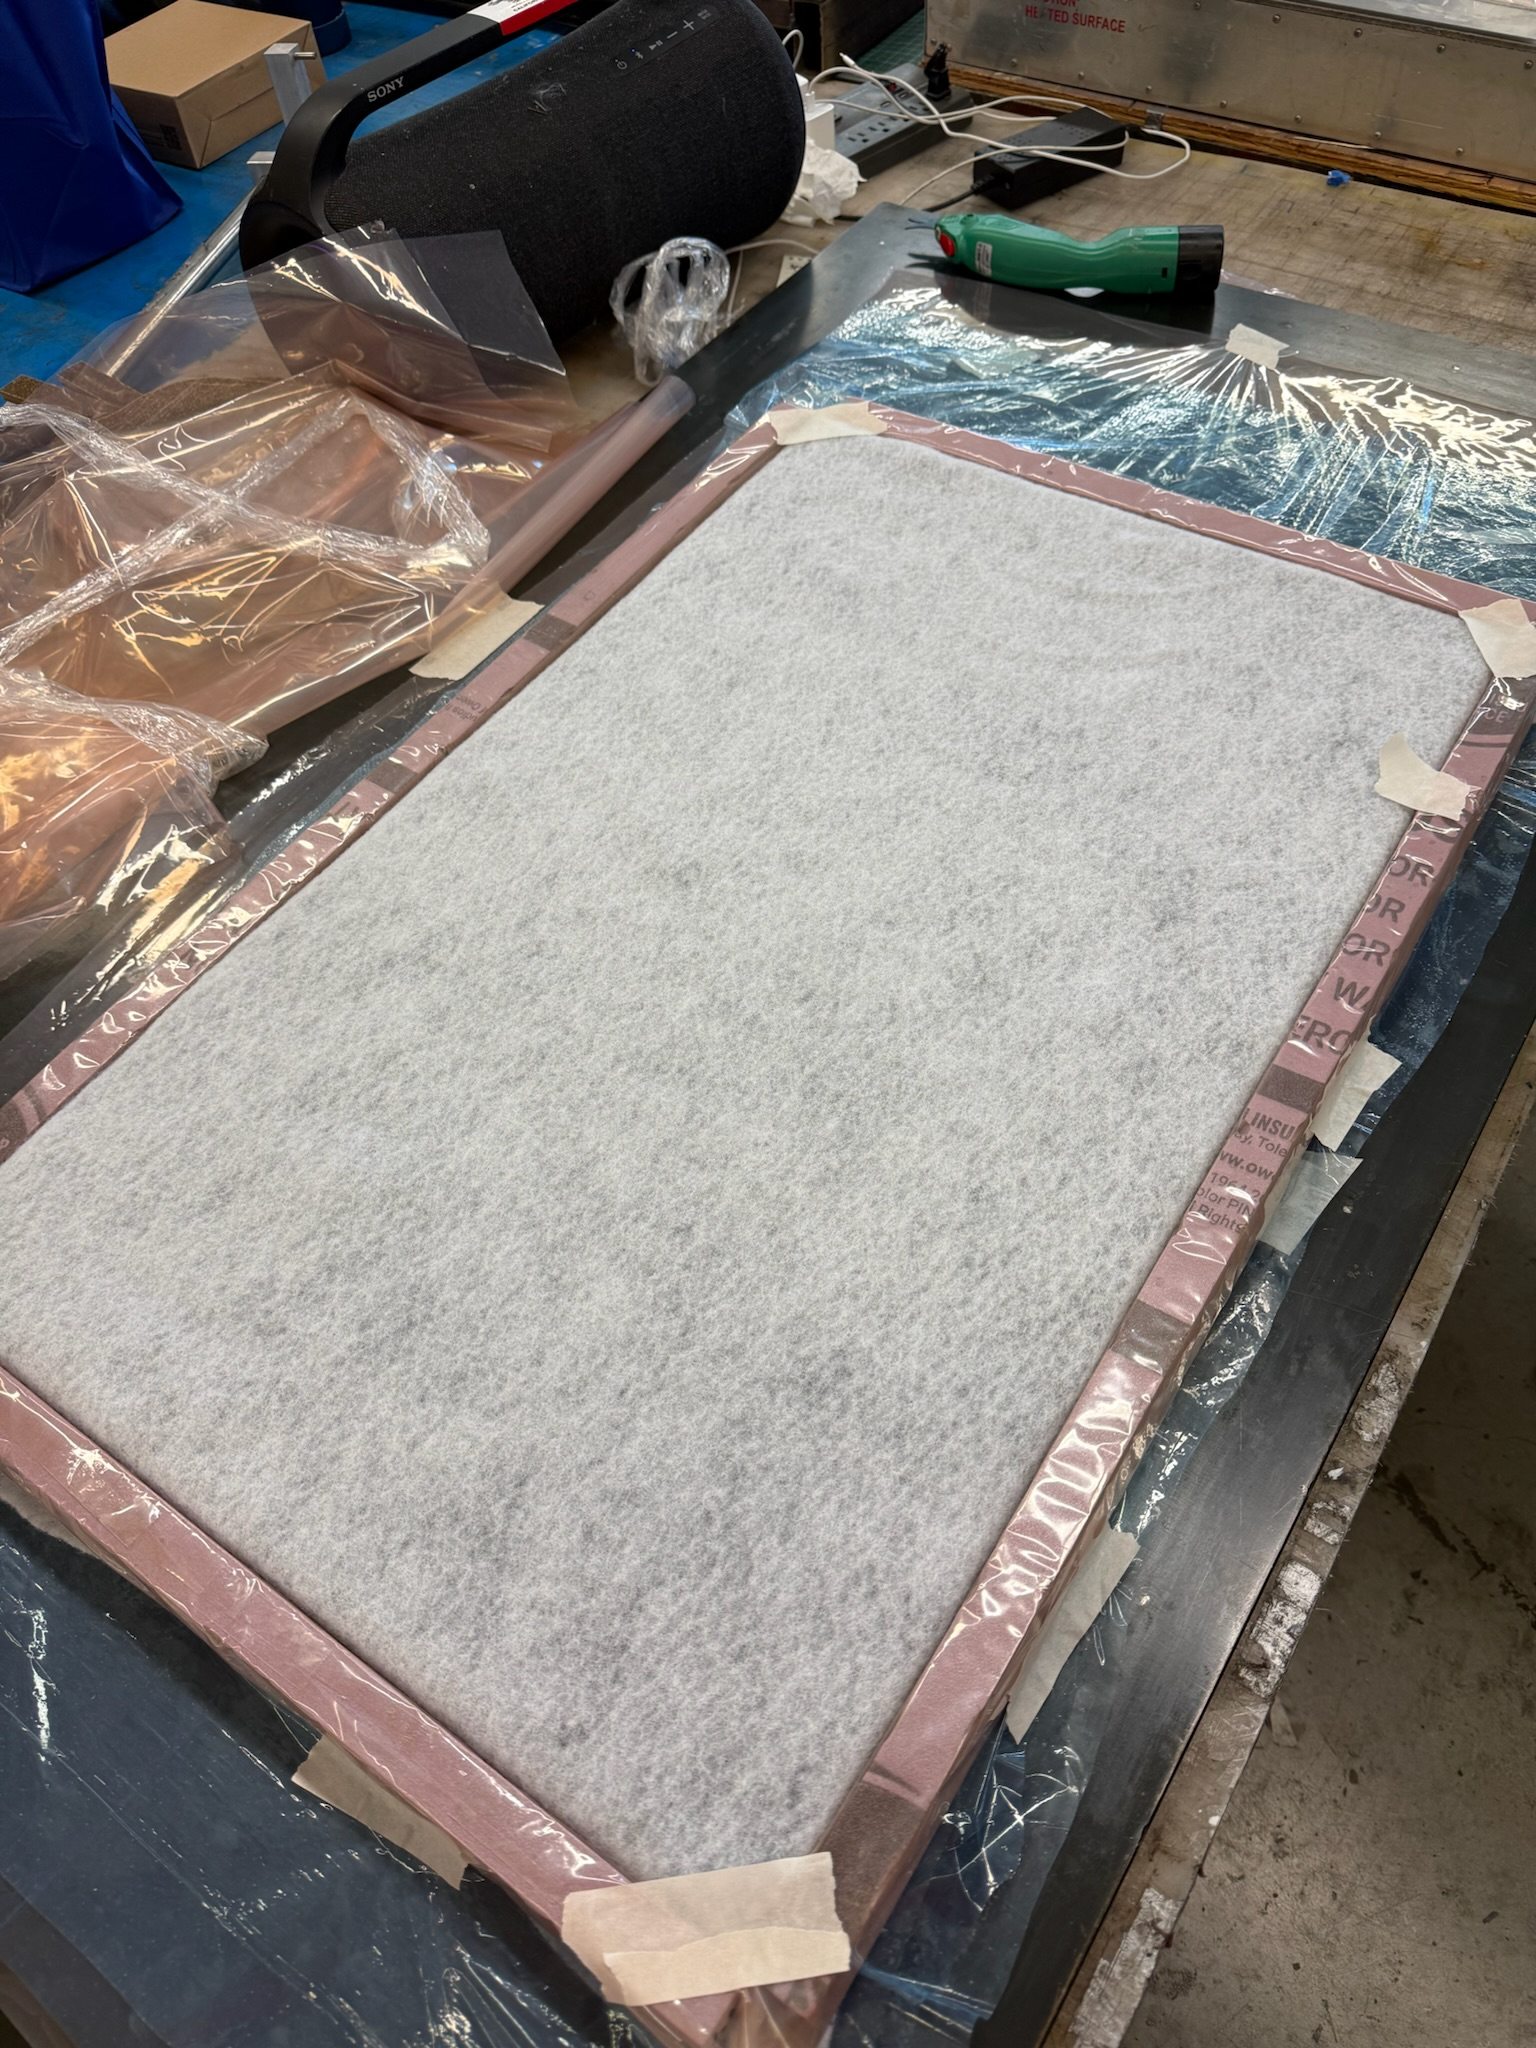
\includegraphics[
        width=3.10in,
        height=1.40in,
        keepaspectratio
    ]{completed_layup}
};
\draw[RuleGray,line width=0.55pt,rounded corners=4pt]
    ($(current page.north west)+(0.43in,-5.13in)$)
    rectangle
    ($(current page.north west)+(3.71in,-6.62in)$);

% Row 2 image 2 — oven chamber used only as a reliable vacuum enclosure; no heat applied
\node[anchor=center,inner sep=0pt]
at ($(current page.north west)+(5.50in,-5.875in)$)
{
    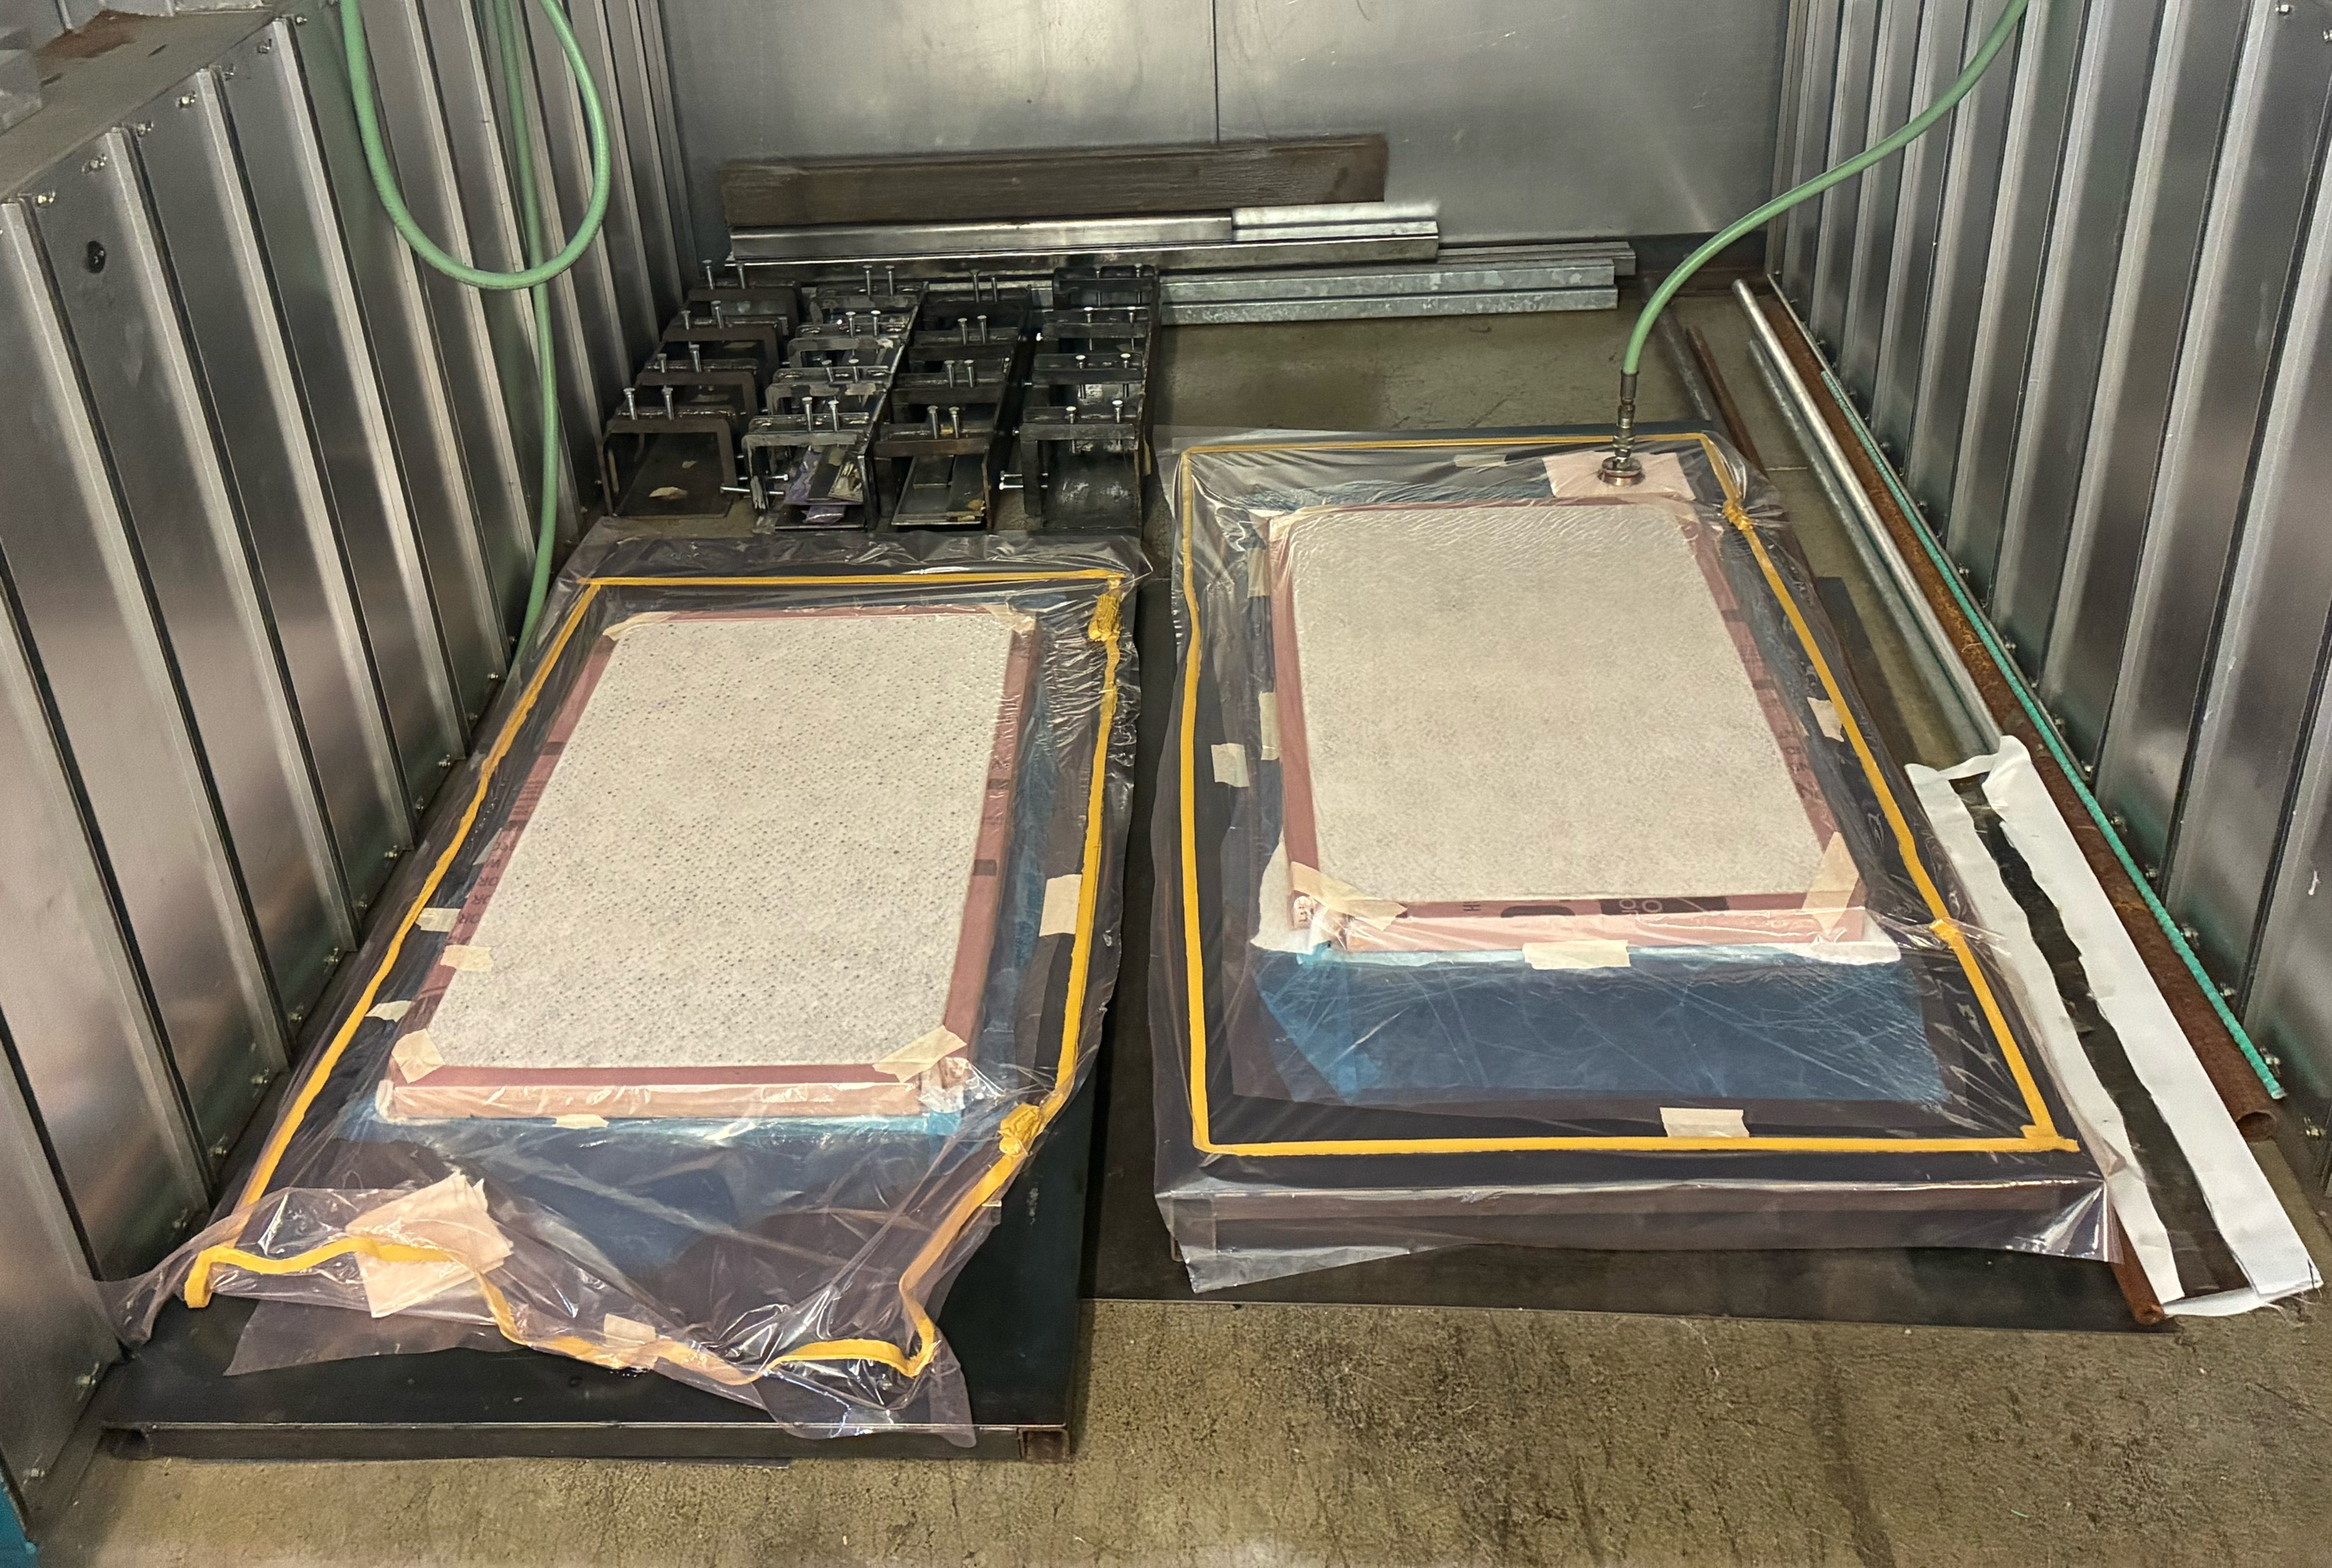
\includegraphics[
        width=3.10in,
        height=1.40in,
        keepaspectratio
    ]{layups_in_composite_oven_under_vacuumPressure}
};
\draw[RuleGray,line width=0.55pt,rounded corners=4pt]
    ($(current page.north west)+(3.86in,-5.13in)$)
    rectangle
    ($(current page.north west)+(7.14in,-6.62in)$);

% Row 2 image 3
\node[anchor=center,inner sep=0pt]
at ($(current page.north west)+(8.935in,-5.875in)$)
{
    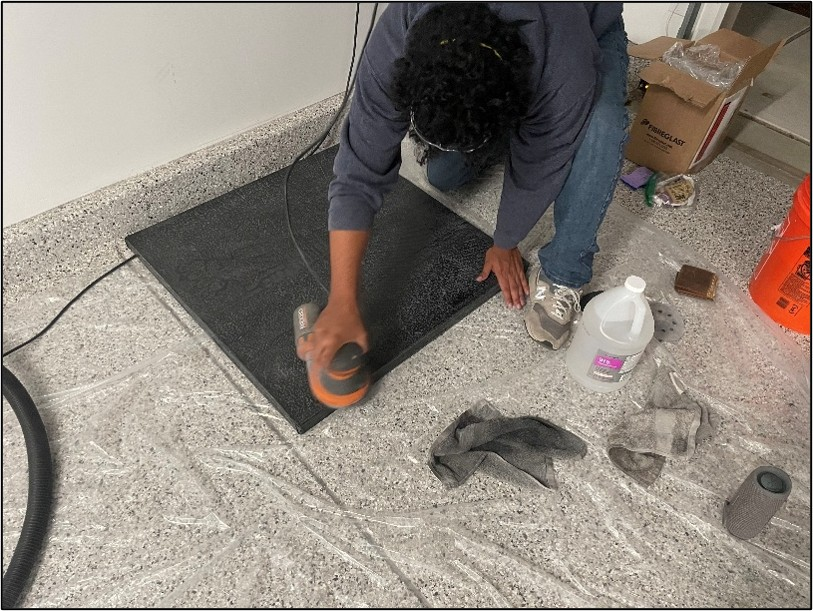
\includegraphics[
        width=3.10in,
        height=1.40in,
        keepaspectratio
    ]{garage_sanding}
};
\draw[RuleGray,line width=0.55pt,rounded corners=4pt]
    ($(current page.north west)+(7.29in,-5.13in)$)
    rectangle
    ($(current page.north east)+(-0.42in,-6.62in)$);

% Row 2 captions
\node[anchor=north,text=Muted,font=\sffamily\fontsize{6.7}{7.3}\selectfont]
at ($(current page.north west)+(2.07in,-6.67in)$)
{4. Fully saturated carbon skin and foam sandwich};

\node[anchor=north,text=Muted,font=\sffamily\fontsize{6.7}{7.3}\selectfont]
at ($(current page.north west)+(5.50in,-6.67in)$)
{5. Room-temperature cure under continuous vacuum};

\node[anchor=north,text=Muted,font=\sffamily\fontsize{6.7}{7.3}\selectfont]
at ($(current page.north west)+(8.935in,-6.67in)$)
{6. Post-processing and surface preparation};

% Bottom callouts
\fill[Panel,rounded corners=4pt]
    ($(current page.north west)+(0.43in,-6.95in)$)
    rectangle
    ($(current page.north west)+(5.48in,-7.60in)$);

\draw[RuleGray,line width=0.55pt,rounded corners=4pt]
    ($(current page.north west)+(0.43in,-6.95in)$)
    rectangle
    ($(current page.north west)+(5.48in,-7.60in)$);

\node[
    anchor=north west,
    text=DeepGreen,
    font=\sffamily\bfseries\fontsize{7.0}{7.6}\selectfont
]
at ($(current page.north west)+(0.63in,-7.08in)$)
{FROM THREE LAYUPS TO ONE};

\node[
    anchor=north west,
    align=left,
    text width=4.56in,
    text=Ink,
    font=\fontsize{6.45}{7.45}\selectfont
]
at ($(current page.north west)+(0.63in,-7.29in)$)
{
The Envelope Method reduced labor, cure cycles, handling,
alignment risk, and time spent forming numerous vacuum-bag
pleats around the 1.5-inch-thick XPS panels.
};

\fill[Panel,rounded corners=4pt]
    ($(current page.north west)+(5.68in,-6.95in)$)
    rectangle
    ($(current page.north east)+(-0.42in,-7.60in)$);

\draw[RuleGray,line width=0.55pt,rounded corners=4pt]
    ($(current page.north west)+(5.68in,-6.95in)$)
    rectangle
    ($(current page.north east)+(-0.42in,-7.60in)$);

\node[
    anchor=north west,
    text=DeepGreen,
    font=\sffamily\bfseries\fontsize{7.0}{7.6}\selectfont
]
at ($(current page.north west)+(5.88in,-7.08in)$)
{WHY SURFACE-BONDED HARDWARE};

\node[
    anchor=north west,
    align=left,
    text width=4.55in,
    text=Ink,
    font=\fontsize{6.45}{7.45}\selectfont
]
at ($(current page.north west)+(5.88in,-7.29in)$)
{
Adhesively bonded hinges and fixtures preserved the clean
composite exterior and avoided drilled inserts, foam-core
crushing, added stress concentrations, and new leak paths.
};


% Footer
\node[
    anchor=south west,
    text=white,
    font=\sffamily\bfseries\fontsize{7.1}{7.7}\selectfont
]
at ($(current page.south west)+(0.42in,0.17in)$)
{\faArrowLeft\ PRODUCT ARCHITECTURE};

\node[
    anchor=south,
    text=white,
    font=\sffamily\fontsize{7.0}{7.6}\selectfont
]
at ($(current page.south)+(0,0.17in)$)
{TORO COVER \hspace{6pt} 2 / 3};

\node[
    anchor=south east,
    text=white,
    font=\sffamily\bfseries\fontsize{7.1}{7.7}\selectfont
]
at ($(current page.south east)+(-0.42in,0.17in)$)
{VALIDATION \& TAKEAWAYS \faArrowRight};

\end{tikzpicture}


% ============================================================
% PAGE 3 — FINISHING, VALIDATION, AND TAKEAWAYS
% ============================================================

\clearpage
\thispagestyle{empty}
\hypertarget{toro-results}{}
\null

\begin{tikzpicture}[remember picture,overlay]

% Background and bars
\fill[white]
    (current page.south west)
    rectangle
    (current page.north east);

\fill[DeepGreen]
    (current page.north west)
    rectangle
    ($(current page.north east)+(0,-0.095in)$);

\fill[PolyGold]
    ($(current page.north west)+(0,-0.095in)$)
    rectangle
    ($(current page.north east)+(0,-0.14in)$);

\fill[DeepGreen]
    (current page.south west)
    rectangle
    ($(current page.south east)+(0,0.36in)$);

\fill[PolyGold]
    ($(current page.south west)+(0,0.36in)$)
    rectangle
    ($(current page.south east)+(0,0.405in)$);

% Header
\node[
    anchor=north west,
    text=PolyGold,
    font=\sffamily\bfseries\fontsize{8.1}{8.7}\selectfont
]
at ($(current page.north west)+(0.42in,-0.39in)$)
{TORO COVER \hspace{5pt}/\hspace{5pt} VALIDATION AND ENGINEERING TAKEAWAYS};

\node[
    anchor=north west,
    text=DeepGreen,
    font=\bfseries\fontsize{22.5}{23.5}\selectfont
]
at ($(current page.north west)+(0.40in,-0.67in)$)
{FROM PROTOTYPE TO PRODUCT PATHWAY};

\node[
    anchor=north west,
    text=Muted,
    font=\sffamily\fontsize{8.7}{9.6}\selectfont
]
at ($(current page.north west)+(0.42in,-1.12in)$)
{Environmental protection, usability testing, scope decisions, and lessons from technical leadership};

\fill[PolyGold]
    ($(current page.north west)+(0.42in,-1.36in)$)
    rectangle
    ($(current page.north west)+(5.8in,-1.315in)$);

% Finishing title
\node[
    anchor=north west,
    text=DeepGreen,
    font=\sffamily\bfseries\fontsize{8.0}{8.7}\selectfont
]
at ($(current page.north west)+(0.43in,-1.62in)$)
{OUTDOOR FINISHING AND ENVIRONMENTAL PROTECTION};

% Image 1
\node[anchor=center,inner sep=0pt]
at ($(current page.north west)+(1.705in,-2.655in)$)
{
    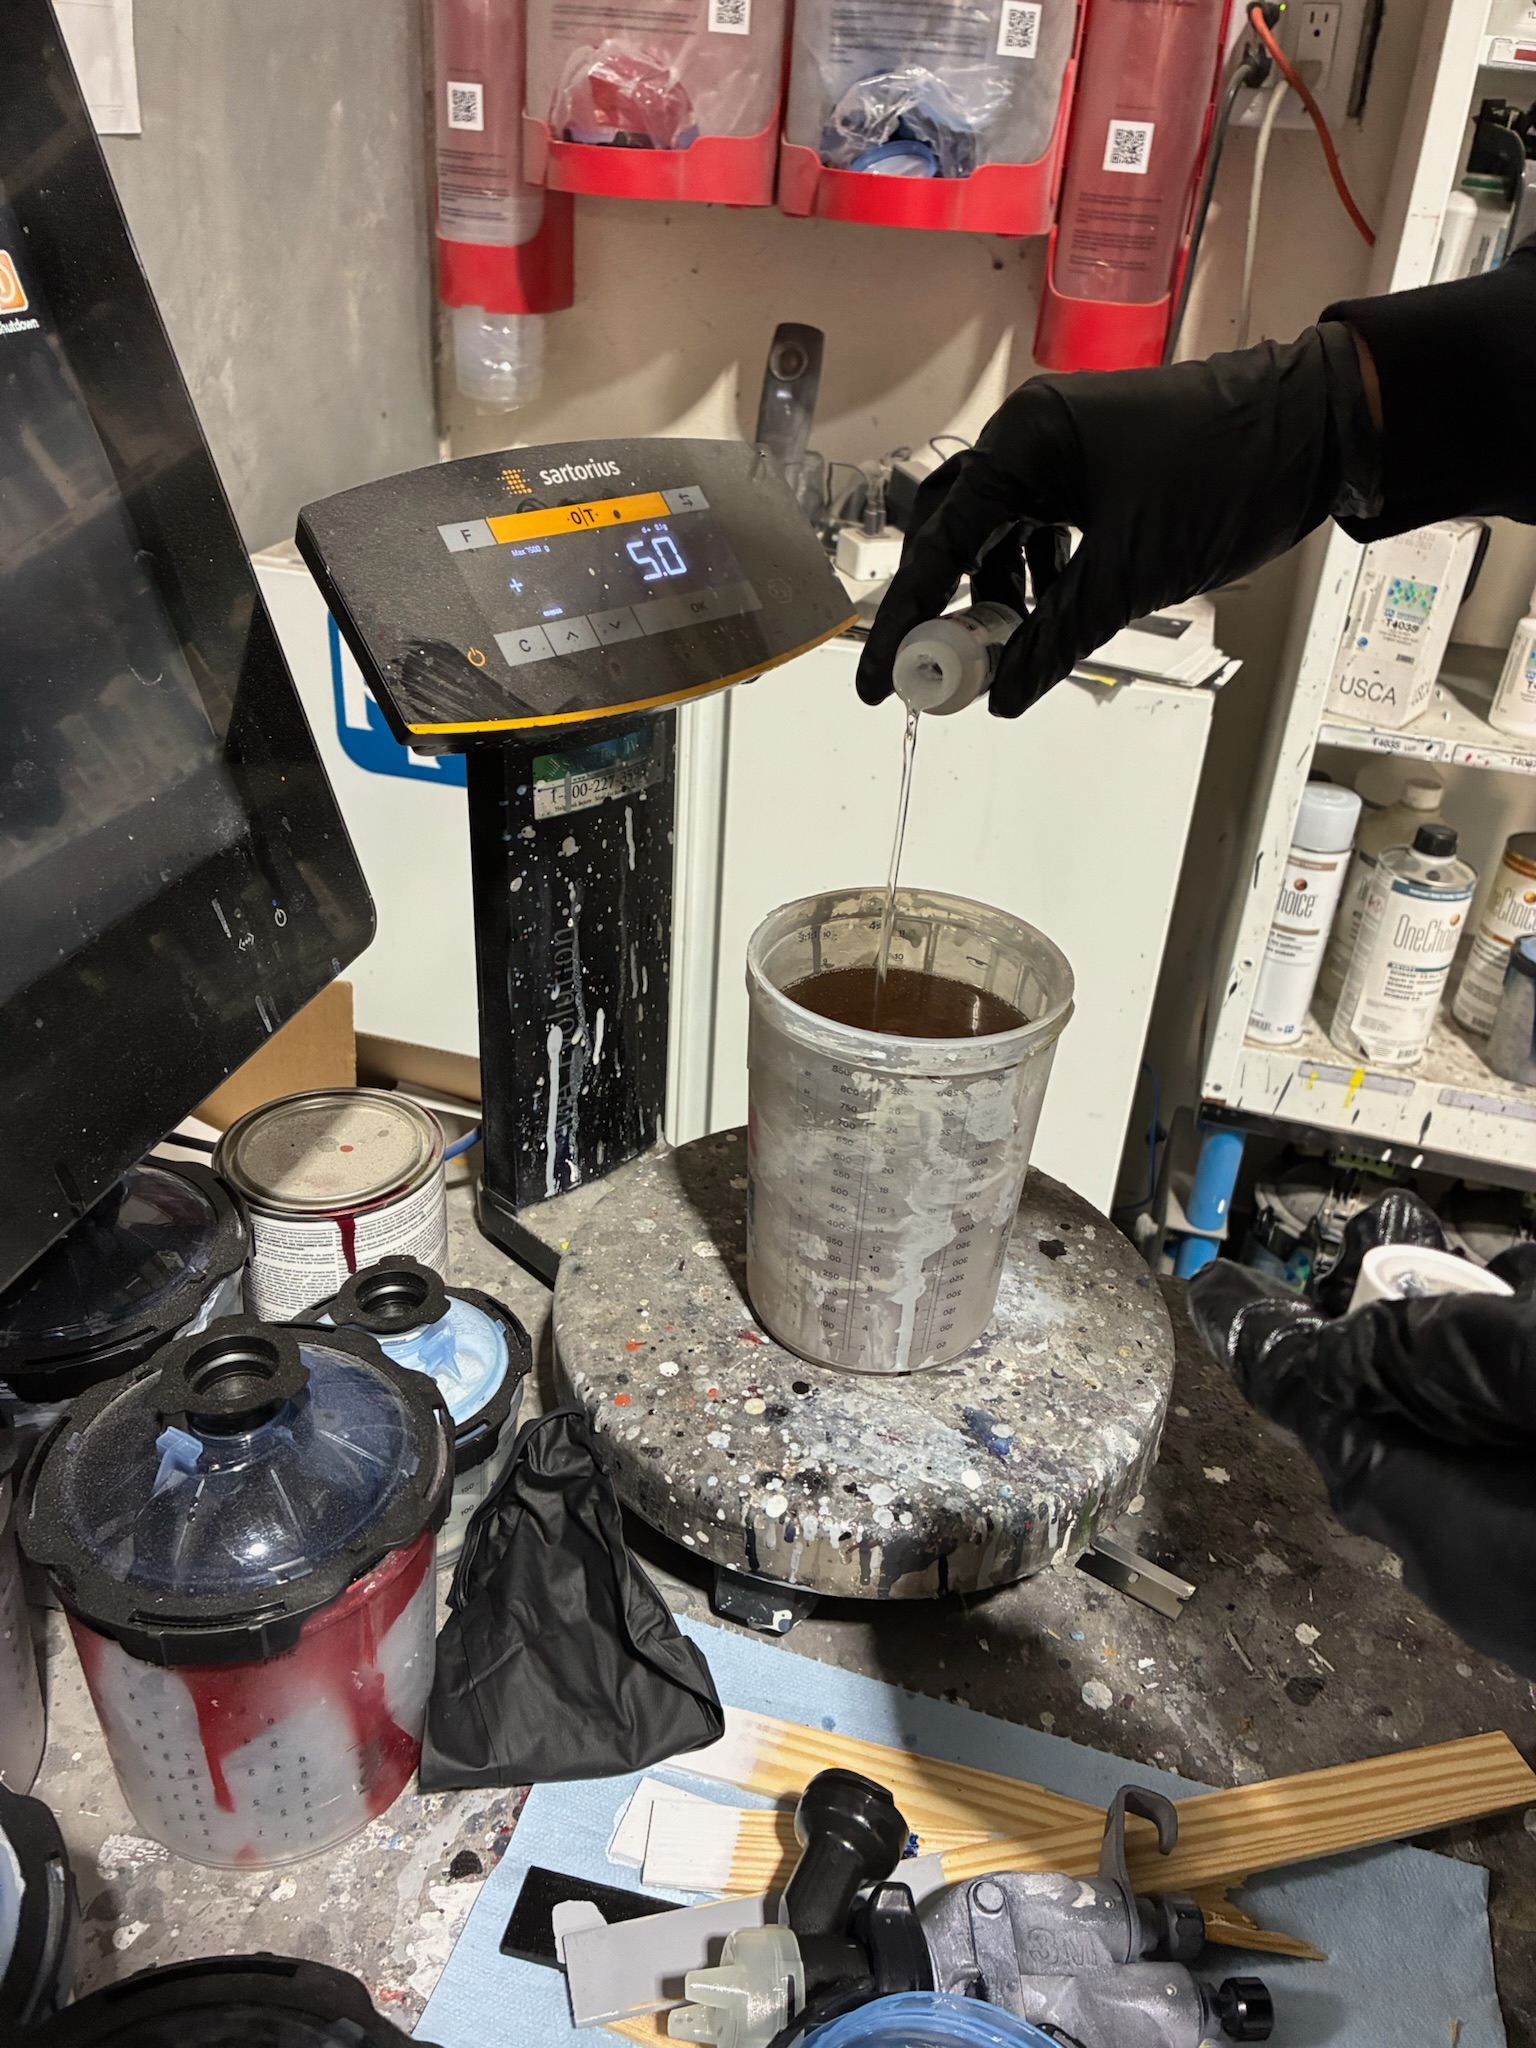
\includegraphics[
        width=2.35in,
        height=1.40in,
        keepaspectratio
    ]{spray_topcoat_prep}
};
\draw[RuleGray,line width=0.55pt,rounded corners=4pt]
    ($(current page.north west)+(0.43in,-1.91in)$)
    rectangle
    ($(current page.north west)+(2.98in,-3.40in)$);

% Image 2
\node[anchor=center,inner sep=0pt]
at ($(current page.north west)+(4.375in,-2.655in)$)
{
    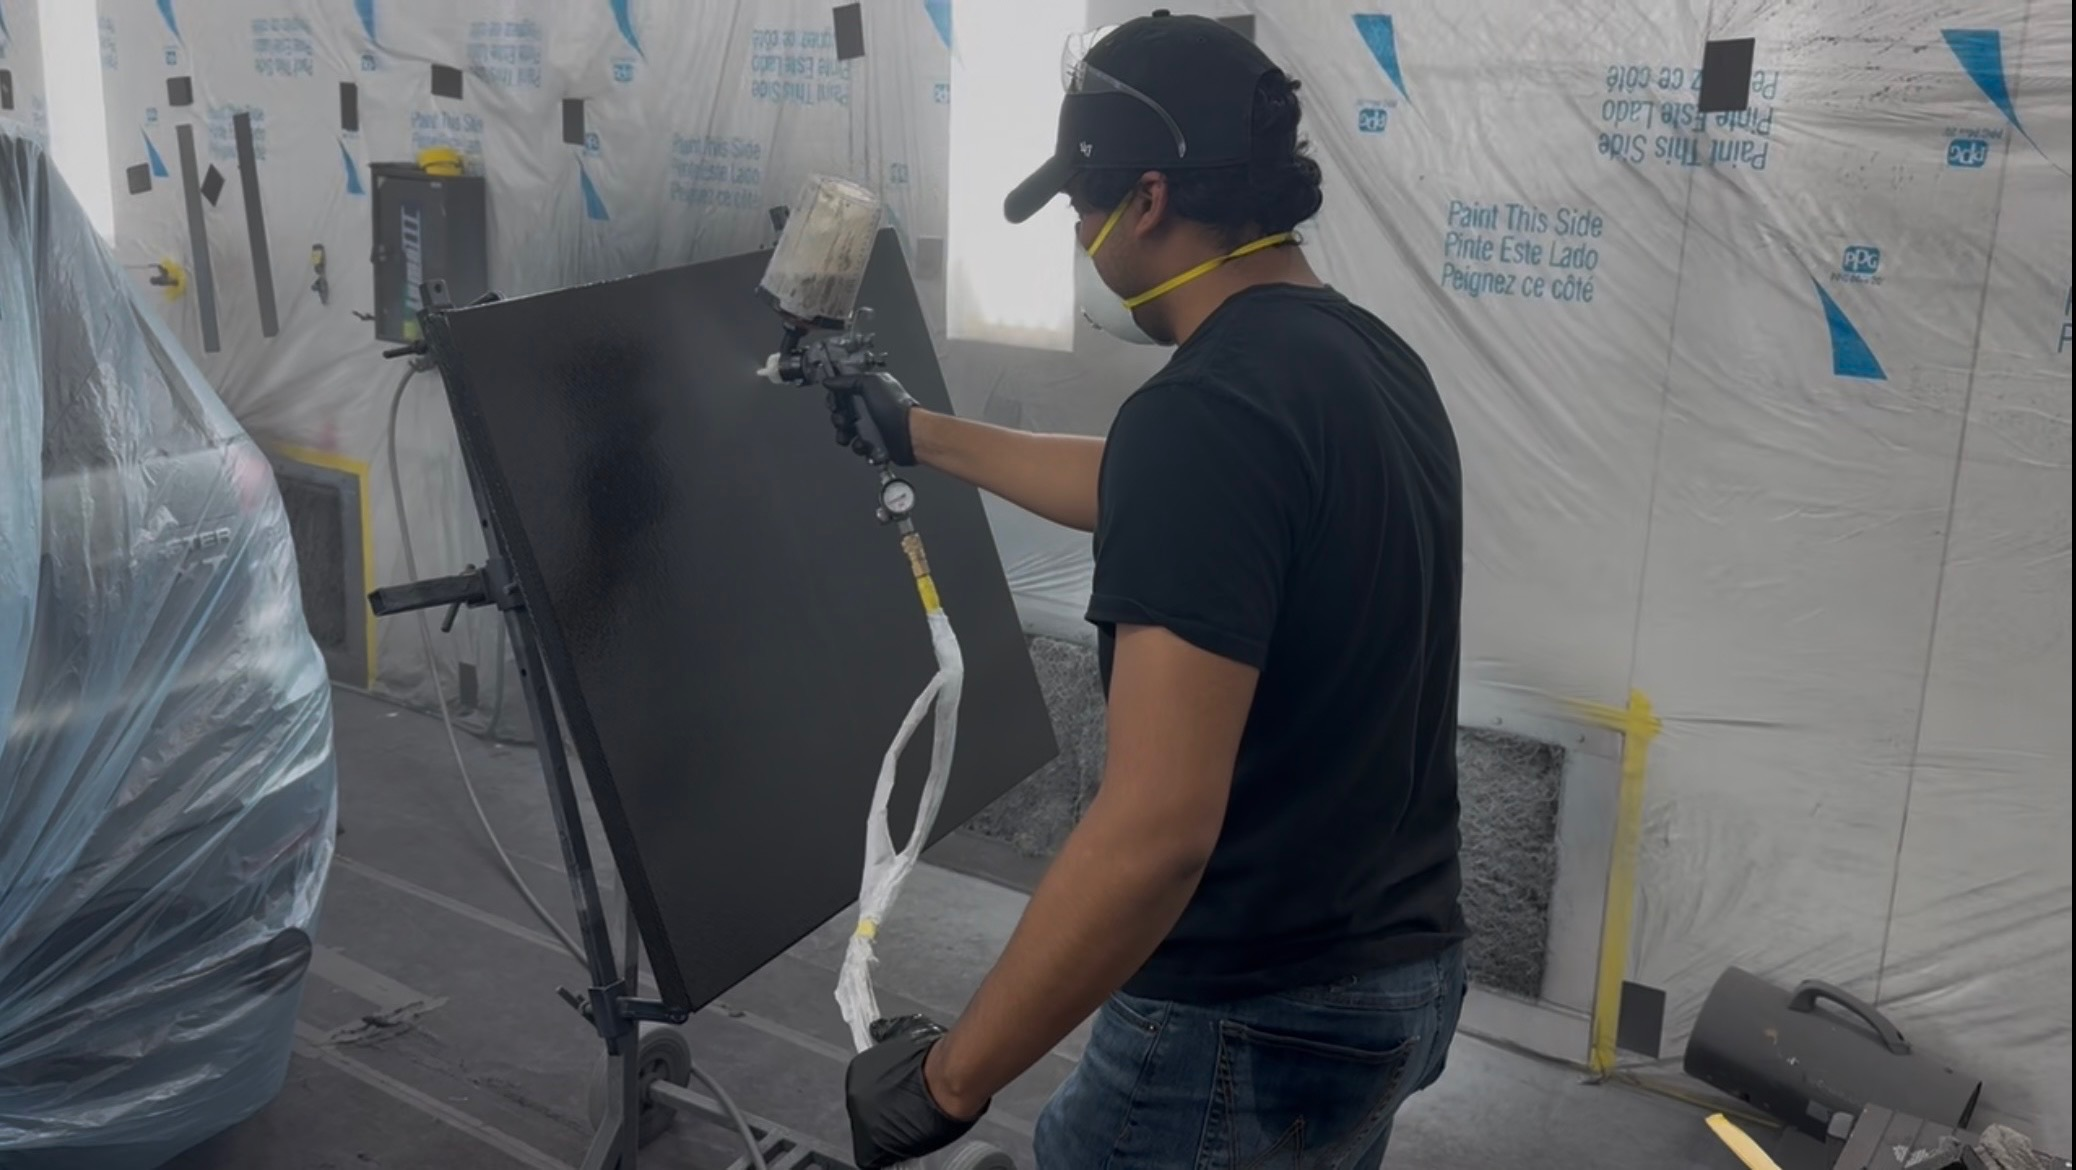
\includegraphics[
        width=2.35in,
        height=1.40in,
        keepaspectratio
    ]{spraying_topcoat}
};
\draw[RuleGray,line width=0.55pt,rounded corners=4pt]
    ($(current page.north west)+(3.10in,-1.91in)$)
    rectangle
    ($(current page.north west)+(5.65in,-3.40in)$);

% Image 3
\node[anchor=center,inner sep=0pt]
at ($(current page.north west)+(7.045in,-2.655in)$)
{
    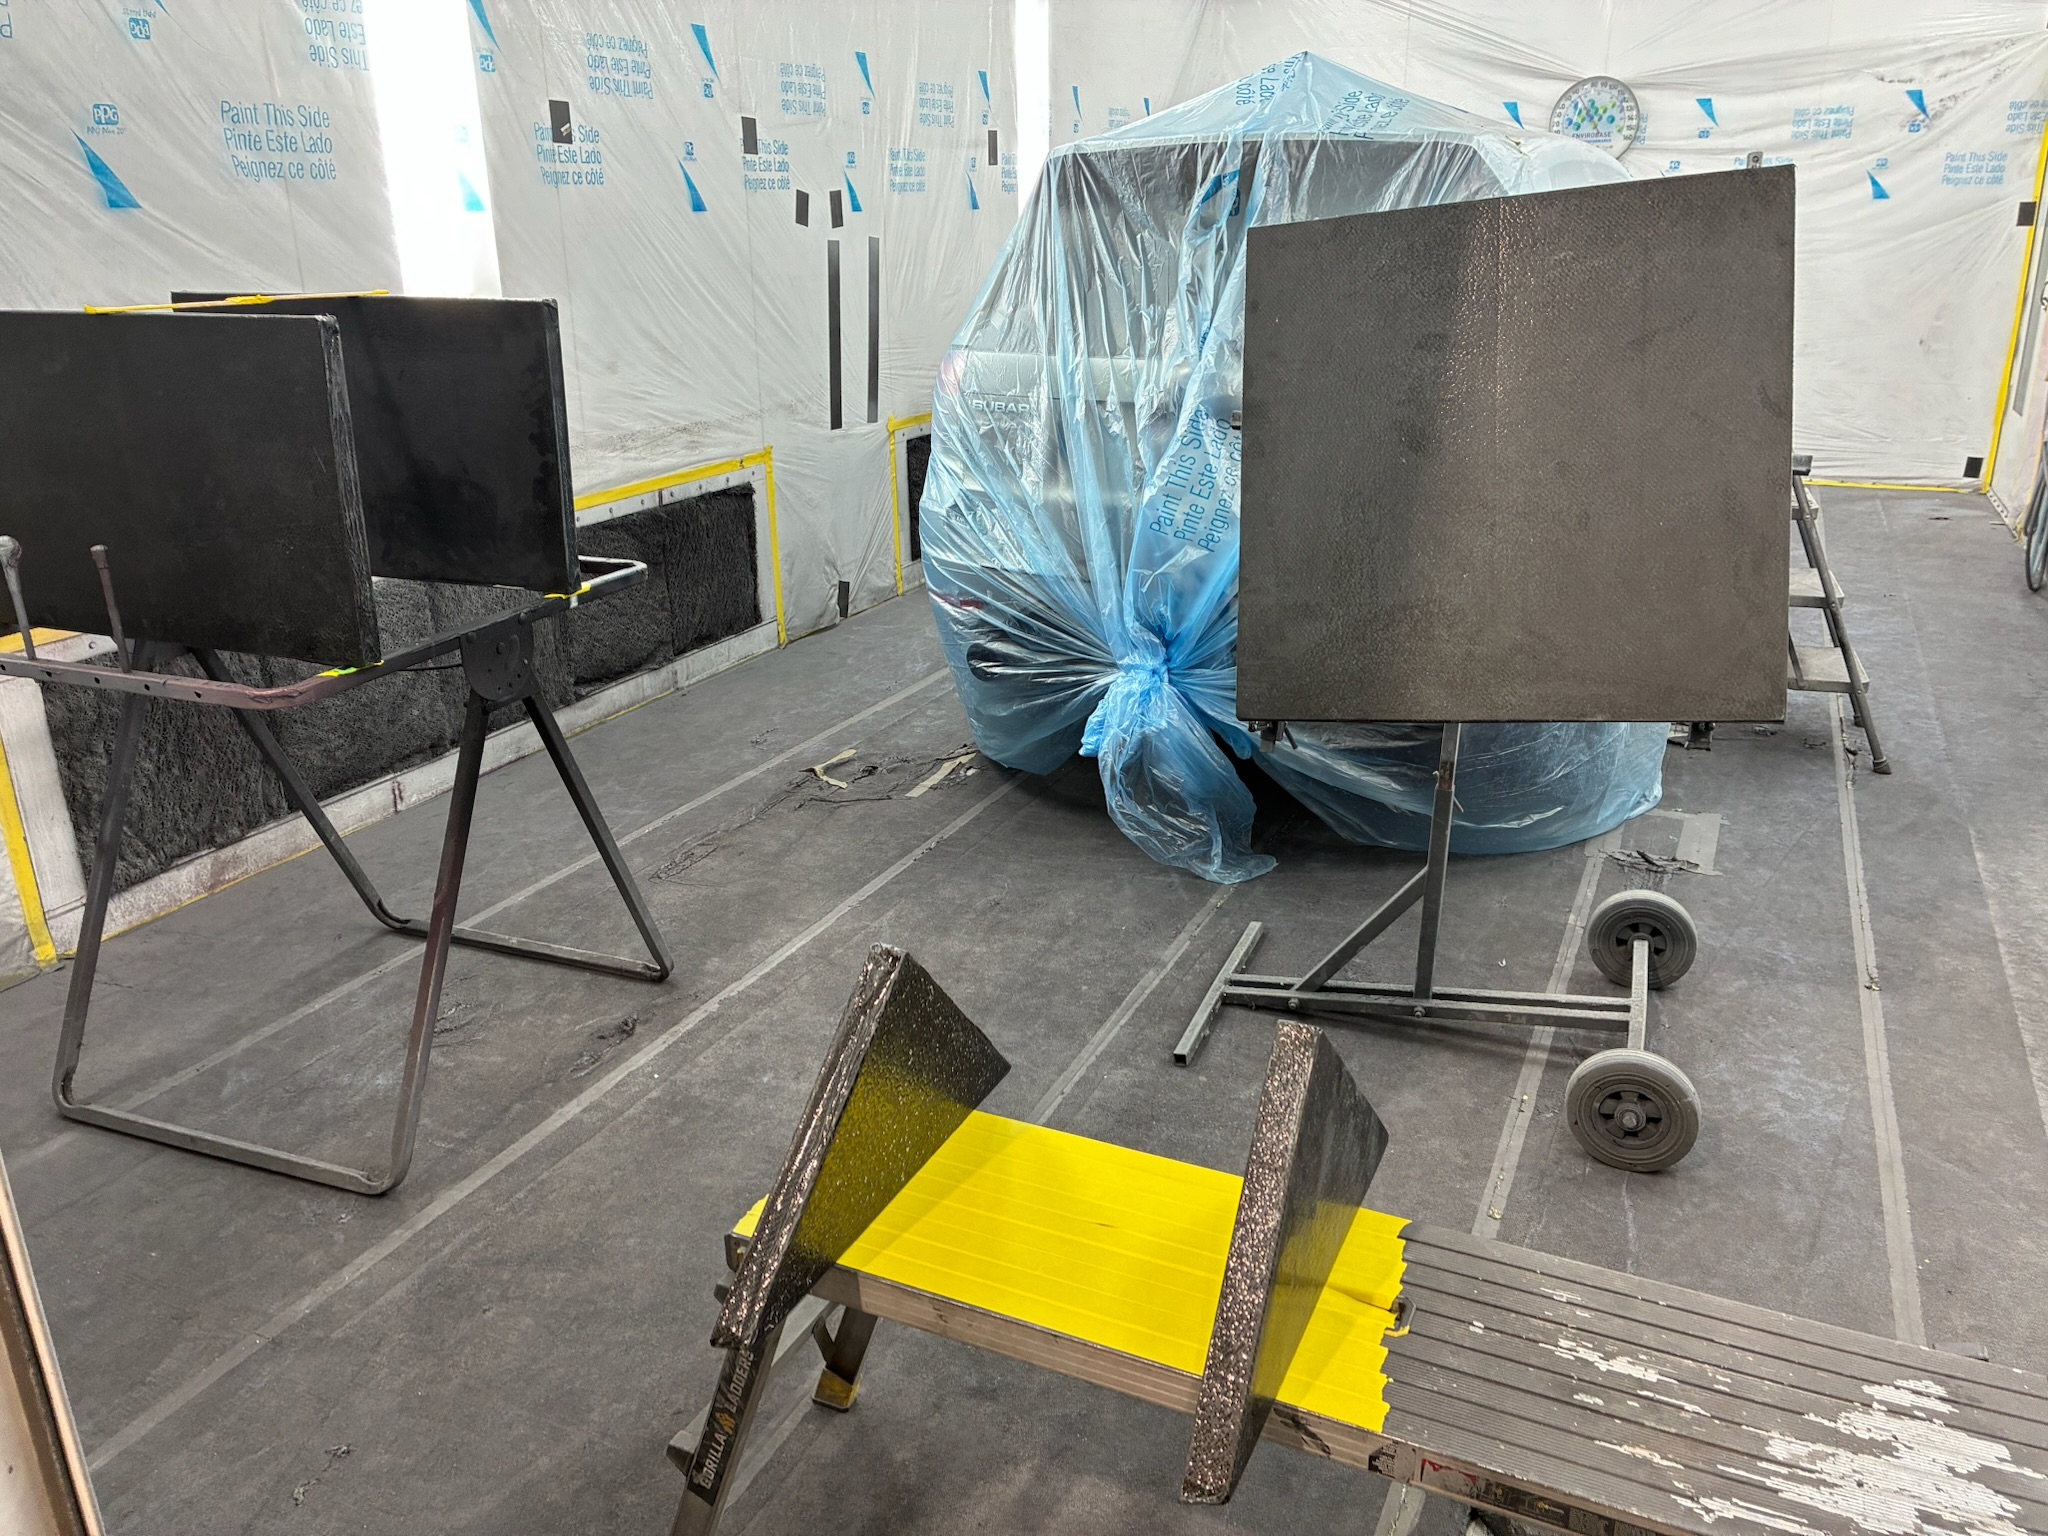
\includegraphics[
        width=2.35in,
        height=1.40in,
        keepaspectratio
    ]{topcoat_setup_apparatus}
};
\draw[RuleGray,line width=0.55pt,rounded corners=4pt]
    ($(current page.north west)+(5.77in,-1.91in)$)
    rectangle
    ($(current page.north west)+(8.32in,-3.40in)$);

% Image 4
\node[anchor=center,inner sep=0pt]
at ($(current page.north west)+(9.50in,-2.655in)$)
{
    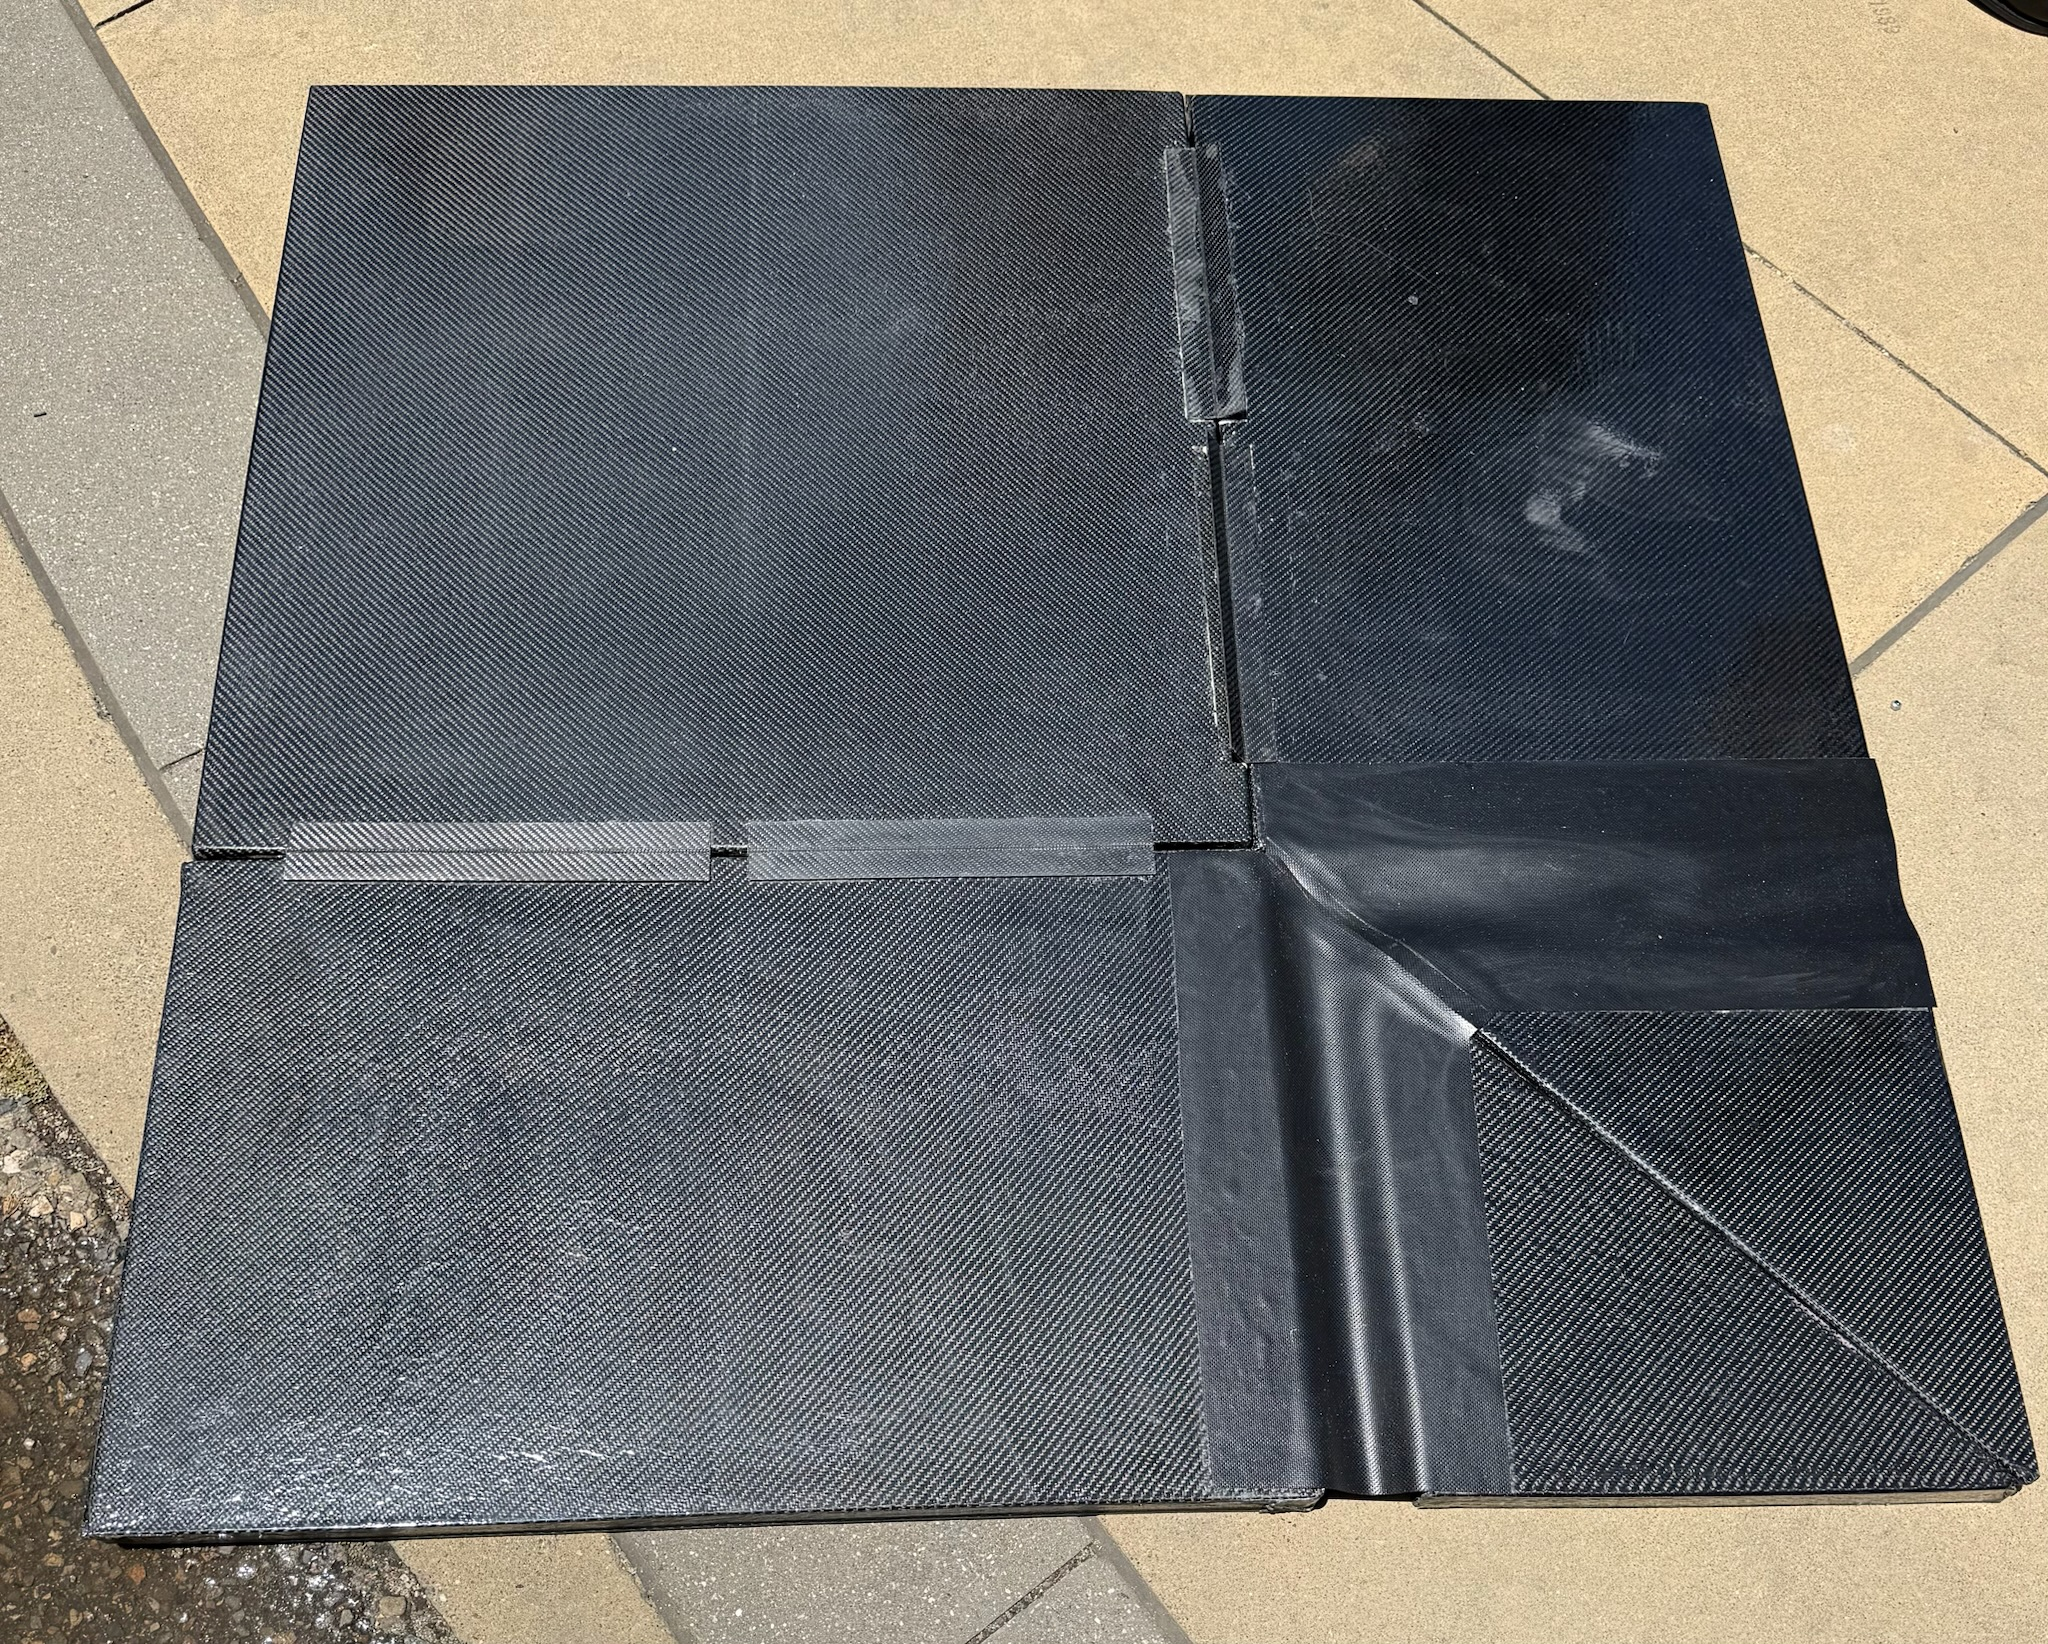
\includegraphics[
        width=2.35in,
        height=1.40in,
        keepaspectratio
    ]{refined_final_toro_cover_partial_carbon_model}
};
\draw[RuleGray,line width=0.55pt,rounded corners=4pt]
    ($(current page.north west)+(8.44in,-1.91in)$)
    rectangle
    ($(current page.north east)+(-0.42in,-3.40in)$);

% Captions
\node[anchor=north,text=Muted,font=\sffamily\fontsize{6.7}{7.3}\selectfont]
at ($(current page.north west)+(1.705in,-3.45in)$)
{Topcoat material preparation};

\node[anchor=north,text=Muted,font=\sffamily\fontsize{6.7}{7.3}\selectfont]
at ($(current page.north west)+(4.375in,-3.45in)$)
{Automotive-booth topcoat application};

\node[anchor=north,text=Muted,font=\sffamily\fontsize{6.7}{7.3}\selectfont]
at ($(current page.north west)+(7.045in,-3.45in)$)
{Coated panels drying after application};

\node[anchor=north,text=Muted,font=\sffamily\fontsize{6.7}{7.3}\selectfont]
at ($(current page.north west)+(9.50in,-3.45in)$)
{Partial carbon manufacturing model};

% Environmental rationale
\fill[SoftGold,rounded corners=4pt]
    ($(current page.north west)+(0.43in,-3.73in)$)
    rectangle
    ($(current page.north east)+(-0.42in,-4.76in)$);

\node[
    anchor=north west,
    align=left,
    text width=9.75in,
    text=Ink,
    font=\fontsize{7.05}{8.25}\selectfont
]
at ($(current page.north west)+(0.65in,-3.89in)$)
{
Because the sponsor required a carbon-fiber cover for outdoor use near chlorinated water,
environmental protection became a functional requirement rather than a cosmetic finish.
I selected and personally sprayed a UV-resistant Sunshield topcoat to seal minor laminate
porosity, reduce moisture ingress, preserve the carbon appearance, limit UV degradation of
the epoxy matrix, and isolate the composite surface from nearby metallic hardware.
};

% Results title
\node[
    anchor=north west,
    text=DeepGreen,
    font=\sffamily\bfseries\fontsize{8.0}{8.7}\selectfont
]
at ($(current page.north west)+(0.43in,-4.94in)$)
{FUNCTIONAL PROTOTYPE RESULTS};

% ------------------------------------------------------------
% Matched lower panels — larger type and improved allocation
% ------------------------------------------------------------

% Left results panel
\fill[SoftGreen,rounded corners=5pt]
    ($(current page.north west)+(0.43in,-5.22in)$)
    rectangle
    ($(current page.north west)+(5.98in,-7.39in)$);

\draw[RuleGray,line width=0.65pt,rounded corners=5pt]
    ($(current page.north west)+(0.43in,-5.22in)$)
    rectangle
    ($(current page.north west)+(5.98in,-7.39in)$);

\fill[DeepGreen,rounded corners=5pt]
    ($(current page.north west)+(0.43in,-5.22in)$)
    rectangle
    ($(current page.north west)+(5.98in,-5.58in)$);

\fill[DeepGreen]
    ($(current page.north west)+(0.43in,-5.40in)$)
    rectangle
    ($(current page.north west)+(5.98in,-5.58in)$);

\node[anchor=west,text=white,
      font=\sffamily\bfseries\fontsize{7.0}{7.6}\selectfont]
at ($(current page.north west)+(0.66in,-5.40in)$)
{SPECIFICATION};

\node[anchor=west,text=white,
      font=\sffamily\bfseries\fontsize{7.0}{7.6}\selectfont]
at ($(current page.north west)+(3.02in,-5.40in)$)
{RESULT};

\node[anchor=east,text=white,
      font=\sffamily\bfseries\fontsize{7.0}{7.6}\selectfont]
at ($(current page.north west)+(5.55in,-5.40in)$)
{STATUS};

\node[
    anchor=north west,
    align=left,
    text width=2.15in,
    text=Ink,
    font=\bfseries\fontsize{7.15}{8.55}\selectfont
]
at ($(current page.north west)+(0.66in,-5.72in)$)
{
Deployment time\\[3.4pt]
Removal time\\[3.4pt]
Single-user operation\\[3.4pt]
Single-side operation\\[3.4pt]
Deployment steps\\[3.4pt]
Removal steps\\[3.4pt]
Weight\\[3.4pt]
Folded storage
};

\node[
    anchor=north west,
    align=left,
    text width=1.45in,
    text=Ink,
    font=\fontsize{7.15}{8.55}\selectfont
]
at ($(current page.north west)+(3.02in,-5.72in)$)
{
25.51 seconds\\[3.4pt]
37.22 seconds\\[3.4pt]
100\% successful\\[3.4pt]
75\% successful\\[3.4pt]
6.4 average\\[3.4pt]
9 average\\[3.4pt]
17 lb\\[3.4pt]
2.9' x 2.9' x 1.7'
};

\node[
    anchor=north east,
    align=right,
    text width=1.05in,
    text=DeepGreen,
    font=\sffamily\bfseries\fontsize{7.05}{8.55}\selectfont
]
at ($(current page.north west)+(5.55in,-5.72in)$)
{
PASS\\[3.4pt]
PASS\\[3.4pt]
PASS\\[3.4pt]
NEAR TARGET\\[3.4pt]
PASS\\[3.4pt]
PASS\\[3.4pt]
NEAR TARGET\\[3.4pt]
PASS
};

% Right takeaways panel — widened for easier reading
\fill[SoftGreen,rounded corners=5pt]
    ($(current page.north west)+(6.14in,-5.22in)$)
    rectangle
    ($(current page.north east)+(-0.42in,-7.39in)$);

\draw[RuleGray,line width=0.65pt,rounded corners=5pt]
    ($(current page.north west)+(6.14in,-5.22in)$)
    rectangle
    ($(current page.north east)+(-0.42in,-7.39in)$);

\fill[DeepGreen,rounded corners=5pt]
    ($(current page.north west)+(6.14in,-5.22in)$)
    rectangle
    ($(current page.north east)+(-0.42in,-5.58in)$);

\fill[DeepGreen]
    ($(current page.north west)+(6.14in,-5.40in)$)
    rectangle
    ($(current page.north east)+(-0.42in,-5.58in)$);

\node[anchor=west,text=white,
      font=\sffamily\bfseries\fontsize{7.1}{7.7}\selectfont]
at ($(current page.north west)+(6.38in,-5.40in)$)
{ENGINEERING TAKEAWAYS};

\node[
    anchor=north west,
    align=left,
    text width=4.02in,
    text=Ink,
    font=\fontsize{6.75}{7.85}\selectfont
]
at ($(current page.north west)+(6.38in,-5.72in)$)
{
\textbf{Manufacturing first.}
Composite manufacturing constraints should guide the product architecture from the beginning.\\[4.5pt]
\textbf{Prioritize deliberately.}
Competing requirements must be balanced intentionally instead of maximizing every objective.\\[4.5pt]
\textbf{Lead through the process.}
Clear procedures, calm communication, and respect for teammates' strengths were essential during fabrication.\\[4.5pt]
\textbf{Next iteration.}
Reduce weight, refine the fabric-hinge fold lines, and improve panel-edge clearance.
};

% Compact concluding pathway
\node[
    anchor=center,
    align=center,
    text=PolyGold,
    font=\sffamily\bfseries\fontsize{6.3}{6.9}\selectfont
]
at ($(current page.north)+(3.06in,-7.18in)$)
{PROTOTYPE \faArrowRight\ DESIGN REFINEMENT
\faArrowRight\ REPEATABLE MANUFACTURING
\faArrowRight\ PRODUCT};

% Validation resources
\node[
    anchor=north,
    align=center,
    text=DeepGreen,
    font=\sffamily\bfseries\fontsize{6.6}{7.2}\selectfont
]
at ($(current page.north)+(0,-7.58in)$)
{\href{\ToroDeploymentLink}{\faPlayCircle\ DEPLOYMENT}
\hspace{18pt}
\href{\ToroRemovalLink}{\faPlayCircle\ REMOVAL / FOLDING}
\hspace{18pt}
\href{\ToroPosterLink}{\faFilePdf\ EXPO POSTER}
\hspace{18pt}
\href{\ToroReportLink}{\faFilePdf\ FINAL REPORT}};

% Footer
\node[
    anchor=south west,
    text=white,
    font=\sffamily\bfseries\fontsize{7.1}{7.7}\selectfont
]
at ($(current page.south west)+(0.42in,0.17in)$)
{\faArrowLeft\ MANUFACTURING-DRIVEN DESIGN};

\node[
    anchor=south,
    text=white,
    font=\sffamily\fontsize{7.0}{7.6}\selectfont
]
at ($(current page.south)+(0,0.17in)$)
{TORO COVER \hspace{6pt} 3 / 3};

\node[
    anchor=south east,
    text=white,
    font=\sffamily\bfseries\fontsize{7.1}{7.7}\selectfont
]
at ($(current page.south east)+(-0.42in,0.17in)$)
{NEXT PROJECT \faArrowRight};

\end{tikzpicture}
\input{paddle}
\clearpage
 before \end{document}.
% 3. Image references use the original Overleaf base filenames
%    without extensions.
% ============================================================



% ============================================================
% CLICKABLE PROJECT RESOURCES
% All links use the exact Google Drive resources supplied.
% ============================================================
\providecommand{\ToroDrawingLink}{https://drive.google.com/file/d/1A7-7wMnRNLuQDaTgxeuUCBsGNqyXzOGV/view?usp=sharing}
\providecommand{\ToroDimensionsLink}{https://drive.google.com/file/d/13sw3BNJvE8GdzlRffxoF2n5r9Gzxide7/view?usp=sharing}
\providecommand{\ToroProblemLink}{https://drive.google.com/file/d/1zHtl8zrb13F1yeN74ptawpfS5UM_xsuw/view?usp=drive_link}
\providecommand{\ToroReportLink}{https://drive.google.com/file/d/1ULZ-P46lFsC2x29ZfmRVIKgYnr9o8hMt/view?usp=drive_link}
\providecommand{\ToroPosterLink}{https://drive.google.com/file/d/1vKiKaJUcHQb_db-FkZnRF6EvtuM4hKyS/view?usp=drive_link}
\providecommand{\ToroDeploymentLink}{https://drive.google.com/file/d/1XJx34o80_mZPTl7xy93HtWAgtS3ThhvY/view?usp=drive_link}
\providecommand{\ToroRemovalLink}{https://drive.google.com/file/d/1O7xYeyB67NUwT-j1B1HeiCcHnZDYjk6_/view?usp=drive_link}

% ============================================================
% PAGE 1 — PROJECT OVERVIEW, OWNERSHIP, AND ARCHITECTURE
% ============================================================

\clearpage
\thispagestyle{empty}
\hypertarget{toro}{}
\null

\begin{tikzpicture}[remember picture,overlay]

% Background
\fill[white]
    (current page.south west)
    rectangle
    (current page.north east);

% Page bars
\fill[DeepGreen]
    (current page.north west)
    rectangle
    ($(current page.north east)+(0,-0.095in)$);

\fill[PolyGold]
    ($(current page.north west)+(0,-0.095in)$)
    rectangle
    ($(current page.north east)+(0,-0.14in)$);

\fill[DeepGreen]
    (current page.south west)
    rectangle
    ($(current page.south east)+(0,0.36in)$);

\fill[PolyGold]
    ($(current page.south west)+(0,0.36in)$)
    rectangle
    ($(current page.south east)+(0,0.405in)$);

% Header
\node[
    anchor=north west,
    text=PolyGold,
    font=\sffamily\bfseries\fontsize{8.1}{8.7}\selectfont
]
at ($(current page.north west)+(0.42in,-0.39in)$)
{01 COMPOSITES \hspace{5pt}/\hspace{5pt} PROJECT 01};

\node[
    anchor=north west,
    text=DeepGreen,
    font=\bfseries\fontsize{23.5}{24.5}\selectfont
]
at ($(current page.north west)+(0.40in,-0.67in)$)
{TORO CARBON FIBER SAFETY COVER};

\node[
    anchor=north west,
    text=Muted,
    font=\sffamily\fontsize{8.4}{9.2}\selectfont
]
at ($(current page.north west)+(0.42in,-1.12in)$)
{Cal Poly Composites Laboratory \hspace{7pt}\textbullet\hspace{7pt}
Team Project \hspace{7pt}\textbullet\hspace{7pt}
Fall--Spring 2026 \hspace{7pt}\textbullet\hspace{7pt}
San Luis Obispo, California};

\fill[PolyGold]
    ($(current page.north west)+(0.42in,-1.37in)$)
    rectangle
    ($(current page.north west)+(6.1in,-1.325in)$);

% Challenge text
\node[
    anchor=north west,
    text=DeepGreen,
    font=\sffamily\bfseries\fontsize{8.1}{8.8}\selectfont
]
at ($(current page.north west)+(0.43in,-1.61in)$)
{THE CHALLENGE};

\node[
    anchor=north west,
    align=left,
    text width=4.47in,
    text=Ink,
    font=\fontsize{8.05}{9.65}\selectfont
]
at ($(current page.north west)+(0.43in,-1.84in)$)
{
Develop a lightweight cover for a 6 ft by 6 ft in-ground spa
that could be deployed by one person, stored compactly,
provide insulation, resist a poolside environment, and maintain
a refined appearance. The sponsor supplied an ambitious but
intentionally broad project statement, requiring the team to
define the product architecture, priorities, manufacturing
strategy, and realistic path toward future commercialization.
};

% Role box
\fill[SoftGold,rounded corners=5pt]
    ($(current page.north west)+(0.42in,-2.88in)$)
    rectangle
    ($(current page.north west)+(4.98in,-4.58in)$);

\fill[PolyGold]
    ($(current page.north west)+(0.42in,-2.88in)$)
    rectangle
    ($(current page.north west)+(0.52in,-4.58in)$);

\node[
    anchor=north west,
    text=DeepGreen,
    font=\sffamily\bfseries\fontsize{8.1}{8.8}\selectfont
]
at ($(current page.north west)+(0.66in,-3.02in)$)
{MY ROLE — DESIGN \& MANUFACTURING LEAD};

\node[
    anchor=north west,
    align=left,
    text width=4.02in,
    text=Ink,
    font=\fontsize{7.05}{8.15}\selectfont
]
at ($(current page.north west)+(0.66in,-3.27in)$)
{
\textbullet\ Modeled every custom part and the complete assembly\\[1.5pt]
\textbullet\ Produced the engineering drawing package independently\\[1.5pt]
\textbullet\ Developed the composite-panel manufacturing process\\[1.5pt]
\textbullet\ Created all waterjet DXFs and manufacturing geometry\\[1.5pt]
\textbullet\ Trained teammates in wet layup and vacuum bagging\\[1.5pt]
\textbullet\ Presented feasibility, scope, and tradeoffs to the sponsor
};

% Large deployed foam-model image
\node[anchor=center,inner sep=0pt]
at ($(current page.north west)+(8.00in,-3.04in)$)
{
    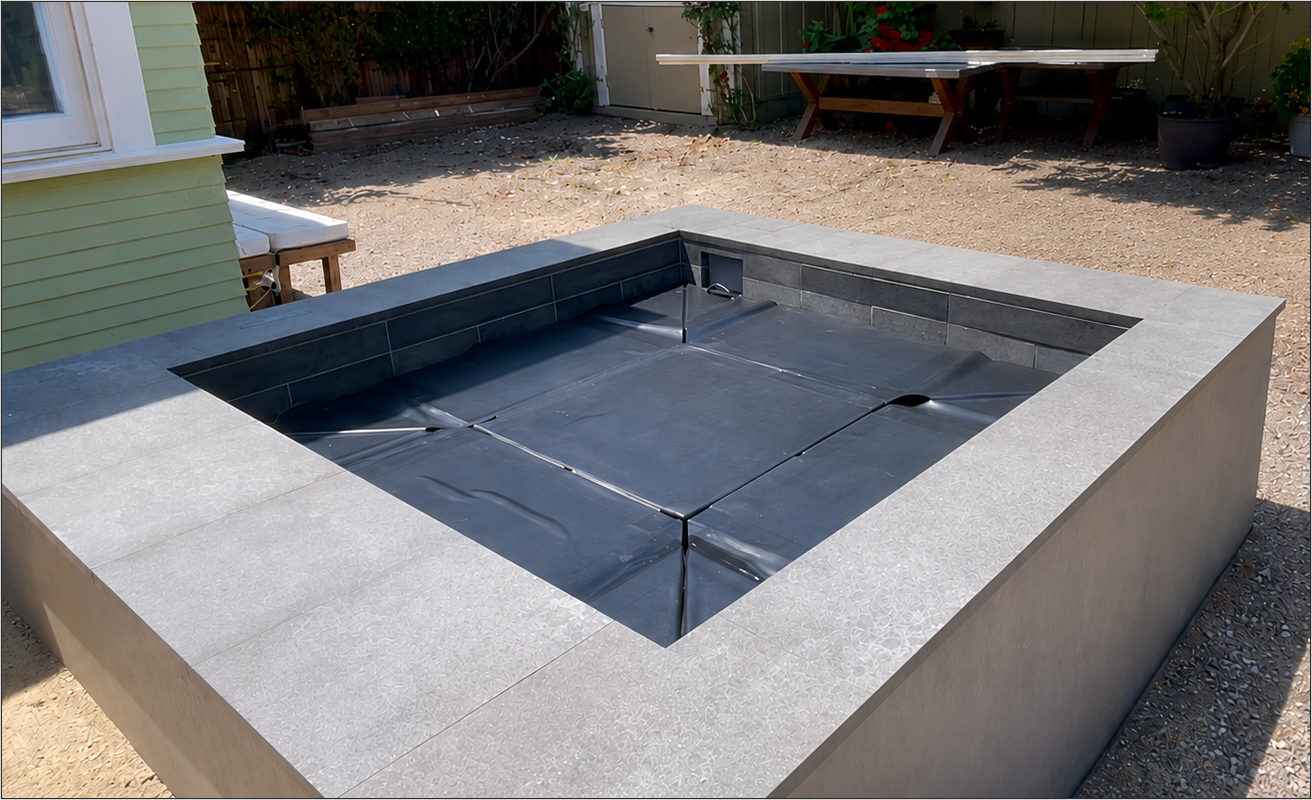
\includegraphics[
        width=5.55in,
        height=2.78in,
        keepaspectratio
    ]{deployed_functional_prototype}
};

\draw[DeepGreen,line width=0.8pt,rounded corners=7pt]
    ($(current page.north west)+(5.16in,-1.61in)$)
    rectangle
    ($(current page.north east)+(-0.42in,-4.47in)$);

\node[
    anchor=north west,
    text=Muted,
    font=\sffamily\fontsize{6.2}{6.9}\selectfont
]
at ($(current page.north west)+(5.18in,-4.54in)$)
{Functional foam model deployed over the sponsor's in-ground spa.};

% Image-strip title
\node[
    anchor=north west,
    text=DeepGreen,
    font=\sffamily\bfseries\fontsize{8.1}{8.8}\selectfont
]
at ($(current page.north west)+(0.43in,-4.78in)$)
{PRODUCT DEVELOPMENT AND FINAL ARCHITECTURE};

% Five-image development strip — CAD-first sequence
% Image 1: topside CAD
\node[anchor=center,inner sep=0pt]
at ($(current page.north west)+(1.47in,-5.73in)$)
{
    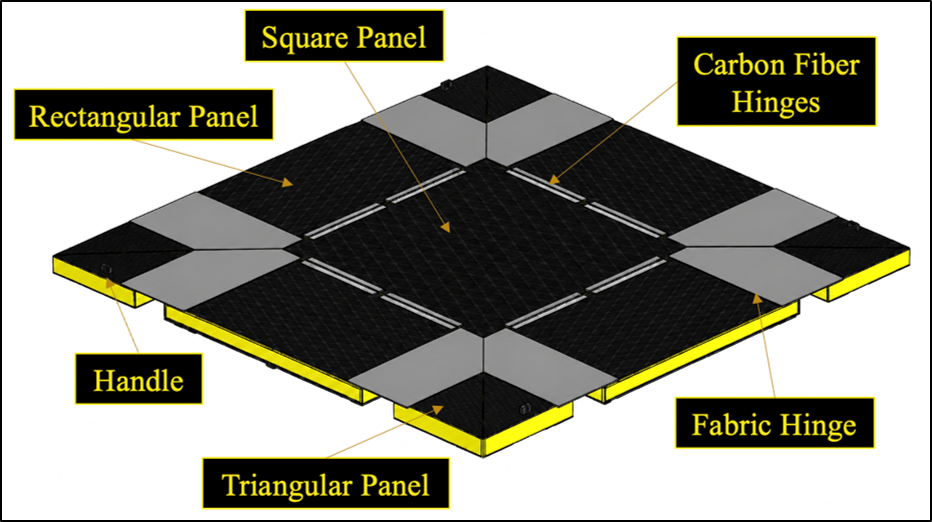
\includegraphics[
        width=1.92in,
        height=1.30in,
        keepaspectratio
    ]{Toro_Cover_topside_Cad}
};
\draw[RuleGray,line width=0.55pt,rounded corners=4pt]
    ($(current page.north west)+(0.43in,-5.04in)$)
    rectangle
    ($(current page.north west)+(2.51in,-6.43in)$);

% Image 2: underside CAD
\node[anchor=center,inner sep=0pt]
at ($(current page.north west)+(3.66in,-5.73in)$)
{
    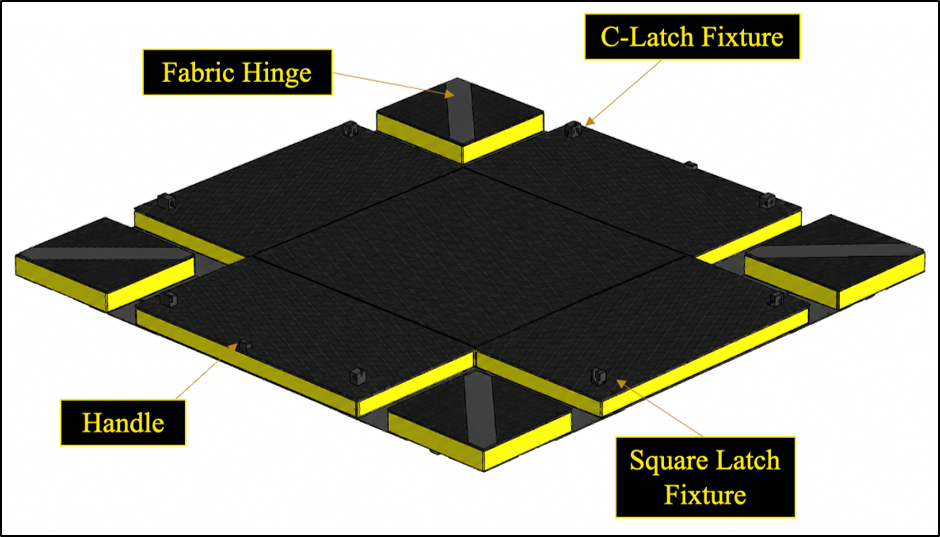
\includegraphics[
        width=1.92in,
        height=1.30in,
        keepaspectratio
    ]{toro_cover_underside_cad}
};
\draw[RuleGray,line width=0.55pt,rounded corners=4pt]
    ($(current page.north west)+(2.62in,-5.04in)$)
    rectangle
    ($(current page.north west)+(4.70in,-6.43in)$);

% Image 3: folded CAD
\node[anchor=center,inner sep=0pt]
at ($(current page.north west)+(5.85in,-5.73in)$)
{
    \includegraphics[
        width=1.92in,
        height=1.30in,
        keepaspectratio
    ]{\detokenize{Toro_Cover_folded Configuration}}
};
\draw[RuleGray,line width=0.55pt,rounded corners=4pt]
    ($(current page.north west)+(4.81in,-5.04in)$)
    rectangle
    ($(current page.north west)+(6.89in,-6.43in)$);

% Image 4: dual-use product concept
\node[anchor=center,inner sep=0pt]
at ($(current page.north west)+(8.04in,-5.73in)$)
{
    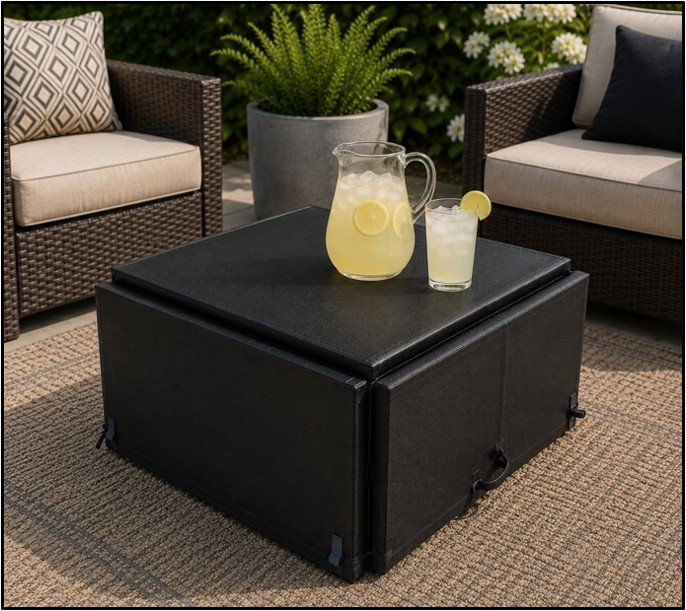
\includegraphics[
        width=1.92in,
        height=1.30in,
        keepaspectratio
    ]{generative_AI_concept_toro_cover_art}
};
\draw[RuleGray,line width=0.55pt,rounded corners=4pt]
    ($(current page.north west)+(7.00in,-5.04in)$)
    rectangle
    ($(current page.north west)+(9.08in,-6.43in)$);

% Image 5: folded foam functional prototype
% The portrait photograph is deliberately clipped to the landscape frame
% so the ottoman fills the card without extending beyond its border.
\begin{scope}
\clip[rounded corners=4pt]
    ($(current page.north west)+(9.19in,-5.04in)$)
    rectangle
    ($(current page.north east)+(-0.43in,-6.43in)$);

% Keep the original image proportions and center it within the existing card.
\node[anchor=center,inner sep=0pt]
at ($(current page.north west)+(9.88in,-5.735in)$)
{
    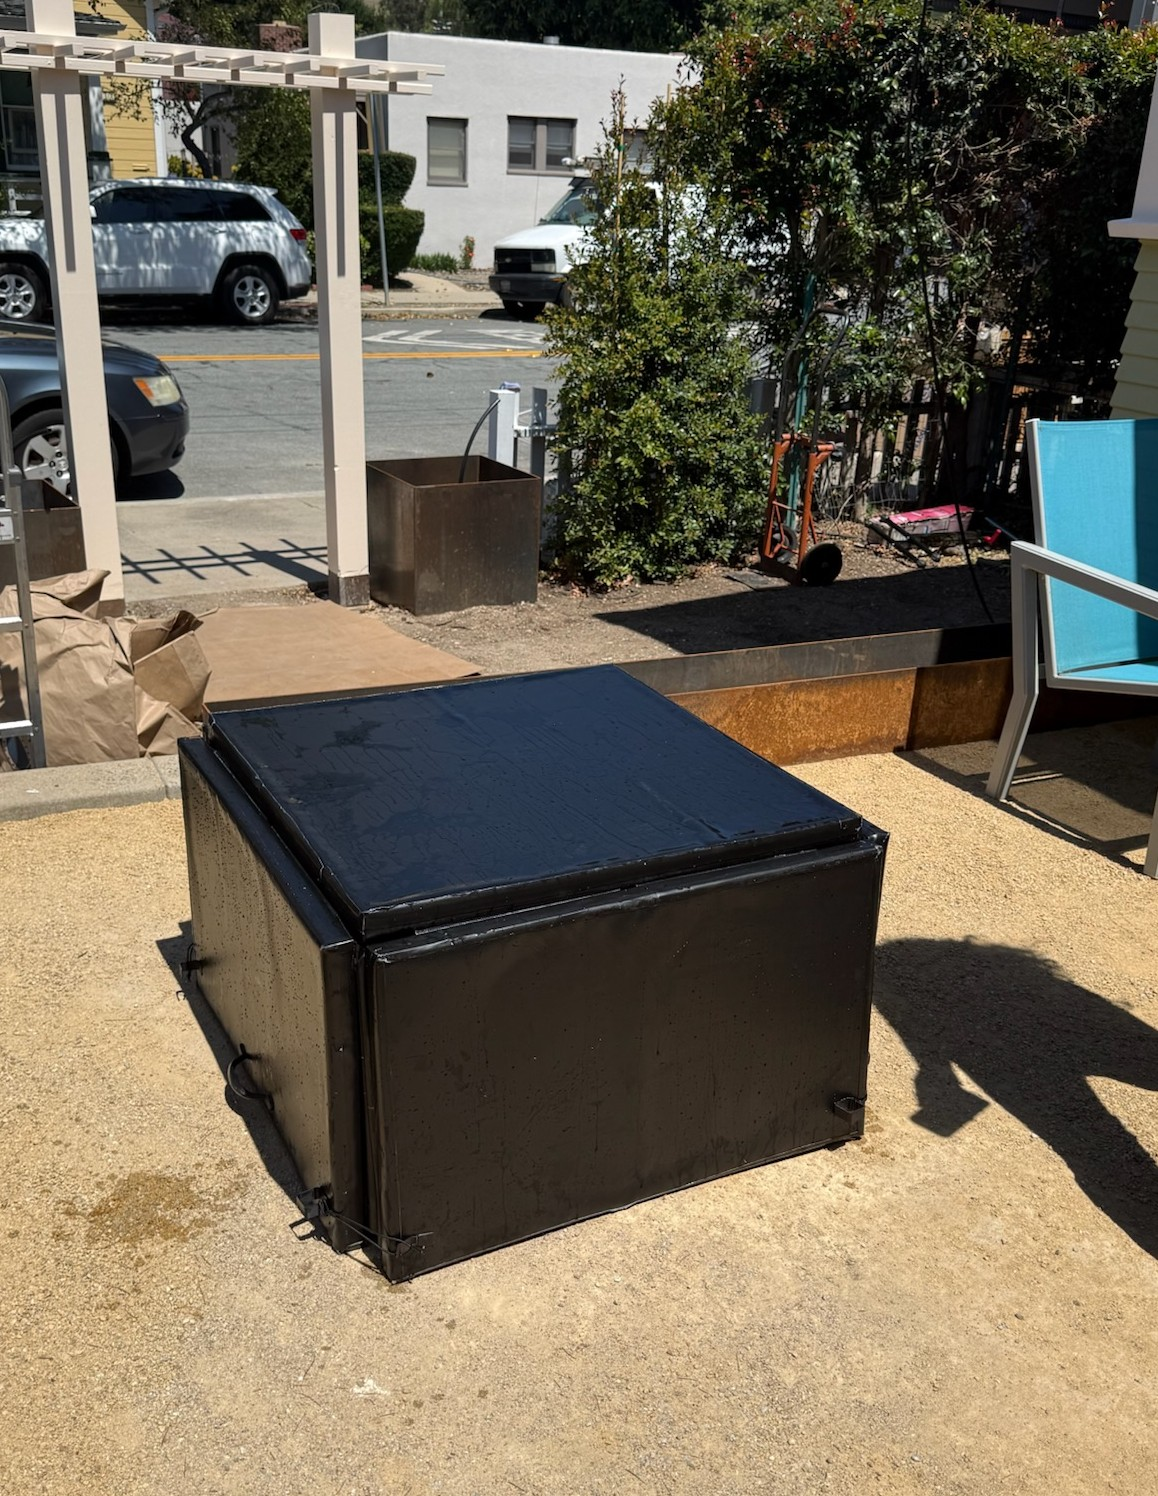
\includegraphics[
        width=1.58in,
        height=1.28in,
        keepaspectratio
    ]{foam_model_folded_backyard_image}
};
\end{scope}

\draw[RuleGray,line width=0.55pt,rounded corners=4pt]
    ($(current page.north west)+(9.19in,-5.04in)$)
    rectangle
    ($(current page.north east)+(-0.43in,-6.43in)$);

% Larger captions
\node[anchor=north,align=center,text width=1.95in,text=Muted,
      font=\sffamily\fontsize{6.8}{7.4}\selectfont]
at ($(current page.north west)+(1.47in,-6.49in)$)
{Topside panel architecture};

\node[anchor=north,align=center,text width=1.95in,text=Muted,
      font=\sffamily\fontsize{6.8}{7.4}\selectfont]
at ($(current page.north west)+(3.66in,-6.49in)$)
{Underside hinge architecture};

\node[anchor=north,align=center,text width=1.95in,text=Muted,
      font=\sffamily\fontsize{6.8}{7.4}\selectfont]
at ($(current page.north west)+(5.85in,-6.49in)$)
{Folded CAD configuration};

\node[anchor=north,align=center,text width=1.95in,text=Muted,
      font=\sffamily\fontsize{6.8}{7.4}\selectfont]
at ($(current page.north west)+(8.04in,-6.49in)$)
{Dual-use product vision};

\node[anchor=north,align=center,text width=1.95in,text=Muted,
      font=\sffamily\fontsize{6.8}{7.4}\selectfont]
at ($(current page.north west)+(9.88in,-6.49in)$)
{Folded foam prototype};

% Page 1 resource bar — centered and non-repeated resources
\fill[Panel,rounded corners=4pt]
    ($(current page.north west)+(0.43in,-7.05in)$)
    rectangle
    ($(current page.north east)+(-0.43in,-7.64in)$);
\draw[RuleGray,line width=0.5pt,rounded corners=4pt]
    ($(current page.north west)+(0.43in,-7.05in)$)
    rectangle
    ($(current page.north east)+(-0.43in,-7.64in)$);

\node[
    anchor=center,
    align=center,
    text=DeepGreen,
    font=\sffamily\bfseries\fontsize{6.9}{7.5}\selectfont
]
at ($(current page.north)+(0,-7.345in)$)
{\href{\ToroDrawingLink}{\faDraftingCompass\ DRAWING PACKAGE}
\hspace{24pt}
\href{\ToroDimensionsLink}{\faImage\ DIMENSION STUDY}
\hspace{24pt}
\href{\ToroProblemLink}{\faFileImage\ PROBLEM STATEMENT}};

% Footer
\node[
    anchor=south west,
    text=white,
    font=\sffamily\bfseries\fontsize{7.1}{7.7}\selectfont
]
at ($(current page.south west)+(0.42in,0.17in)$)
{\hyperlink{composites}{\faArrowLeft\ COMPOSITES}};

\node[
    anchor=south,
    text=white,
    font=\sffamily\fontsize{7.0}{7.6}\selectfont
]
at ($(current page.south)+(0,0.17in)$)
{TORO COVER \hspace{6pt} 1 / 3};

\node[
    anchor=south east,
    text=white,
    font=\sffamily\bfseries\fontsize{7.1}{7.7}\selectfont
]
at ($(current page.south east)+(-0.42in,0.17in)$)
{MANUFACTURING-DRIVEN DESIGN \faArrowRight};

\end{tikzpicture}


% ============================================================
% PAGE 2 — MANUFACTURING-DRIVEN DESIGN
% ============================================================

\clearpage
\thispagestyle{empty}
\hypertarget{toro-manufacturing}{}
\null

\begin{tikzpicture}[remember picture,overlay]

% Background and bars
\fill[white]
    (current page.south west)
    rectangle
    (current page.north east);

\fill[DeepGreen]
    (current page.north west)
    rectangle
    ($(current page.north east)+(0,-0.095in)$);

\fill[PolyGold]
    ($(current page.north west)+(0,-0.095in)$)
    rectangle
    ($(current page.north east)+(0,-0.14in)$);

\fill[DeepGreen]
    (current page.south west)
    rectangle
    ($(current page.south east)+(0,0.36in)$);

\fill[PolyGold]
    ($(current page.south west)+(0,0.36in)$)
    rectangle
    ($(current page.south east)+(0,0.405in)$);

% Header
\node[
    anchor=north west,
    text=PolyGold,
    font=\sffamily\bfseries\fontsize{8.1}{8.7}\selectfont
]
at ($(current page.north west)+(0.42in,-0.39in)$)
{TORO COVER \hspace{5pt}/\hspace{5pt} DESIGN FOR MANUFACTURABILITY};

\node[
    anchor=north west,
    text=DeepGreen,
    font=\bfseries\fontsize{23}{24}\selectfont
]
at ($(current page.north west)+(0.40in,-0.67in)$)
{THE ENVELOPE METHOD};

\node[
    anchor=north west,
    text=Muted,
    font=\sffamily\fontsize{8.7}{9.6}\selectfont
]
at ($(current page.north west)+(0.42in,-1.12in)$)
{A one-layup process developed for unusually thick insulated composite sandwich panels};

\fill[PolyGold]
    ($(current page.north west)+(0.42in,-1.36in)$)
    rectangle
    ($(current page.north west)+(5.30in,-1.315in)$);

% Process explanation
\fill[SoftGold,rounded corners=5pt]
    ($(current page.north west)+(0.42in,-1.61in)$)
    rectangle
    ($(current page.north east)+(-0.42in,-2.90in)$);

\fill[PolyGold]
    ($(current page.north west)+(0.42in,-1.61in)$)
    rectangle
    ($(current page.north west)+(0.52in,-2.90in)$);

\node[
    anchor=north west,
    text=DeepGreen,
    font=\sffamily\bfseries\fontsize{7.9}{8.6}\selectfont
]
at ($(current page.north west)+(0.67in,-1.76in)$)
{PROCESS INNOVATION};

\node[
    anchor=north west,
    align=left,
    text width=9.55in,
    text=Ink,
    font=\fontsize{7.35}{8.75}\selectfont
]
at ($(current page.north west)+(0.67in,-2.02in)$)
{
Weight reduction and insulation were both essential, leading to the selection of an
XPS foam core. Because XPS could not tolerate composite heat-cure temperatures, prepreg
processing was not practical and the panels had to be manufactured by wet layup with a
room-temperature cure. To simplify this process, I waterjet-cut XPS perimeter strips from
excess foam and placed them around each core inside the vacuum enclosure. Under vacuum,
the top and bottom carbon skins met along the panel sides and compressed against this
border, eliminating a separate edge-banding layup and reducing corner pleating.
};

% Workflow title
\node[
    anchor=north west,
    text=DeepGreen,
    font=\sffamily\bfseries\fontsize{8.0}{8.7}\selectfont
]
at ($(current page.north west)+(0.43in,-3.06in)$)
{MANUFACTURING WORKFLOW};

% Row 1 image 1
\node[anchor=center,inner sep=0pt]
at ($(current page.north west)+(2.07in,-4.105in)$)
{
    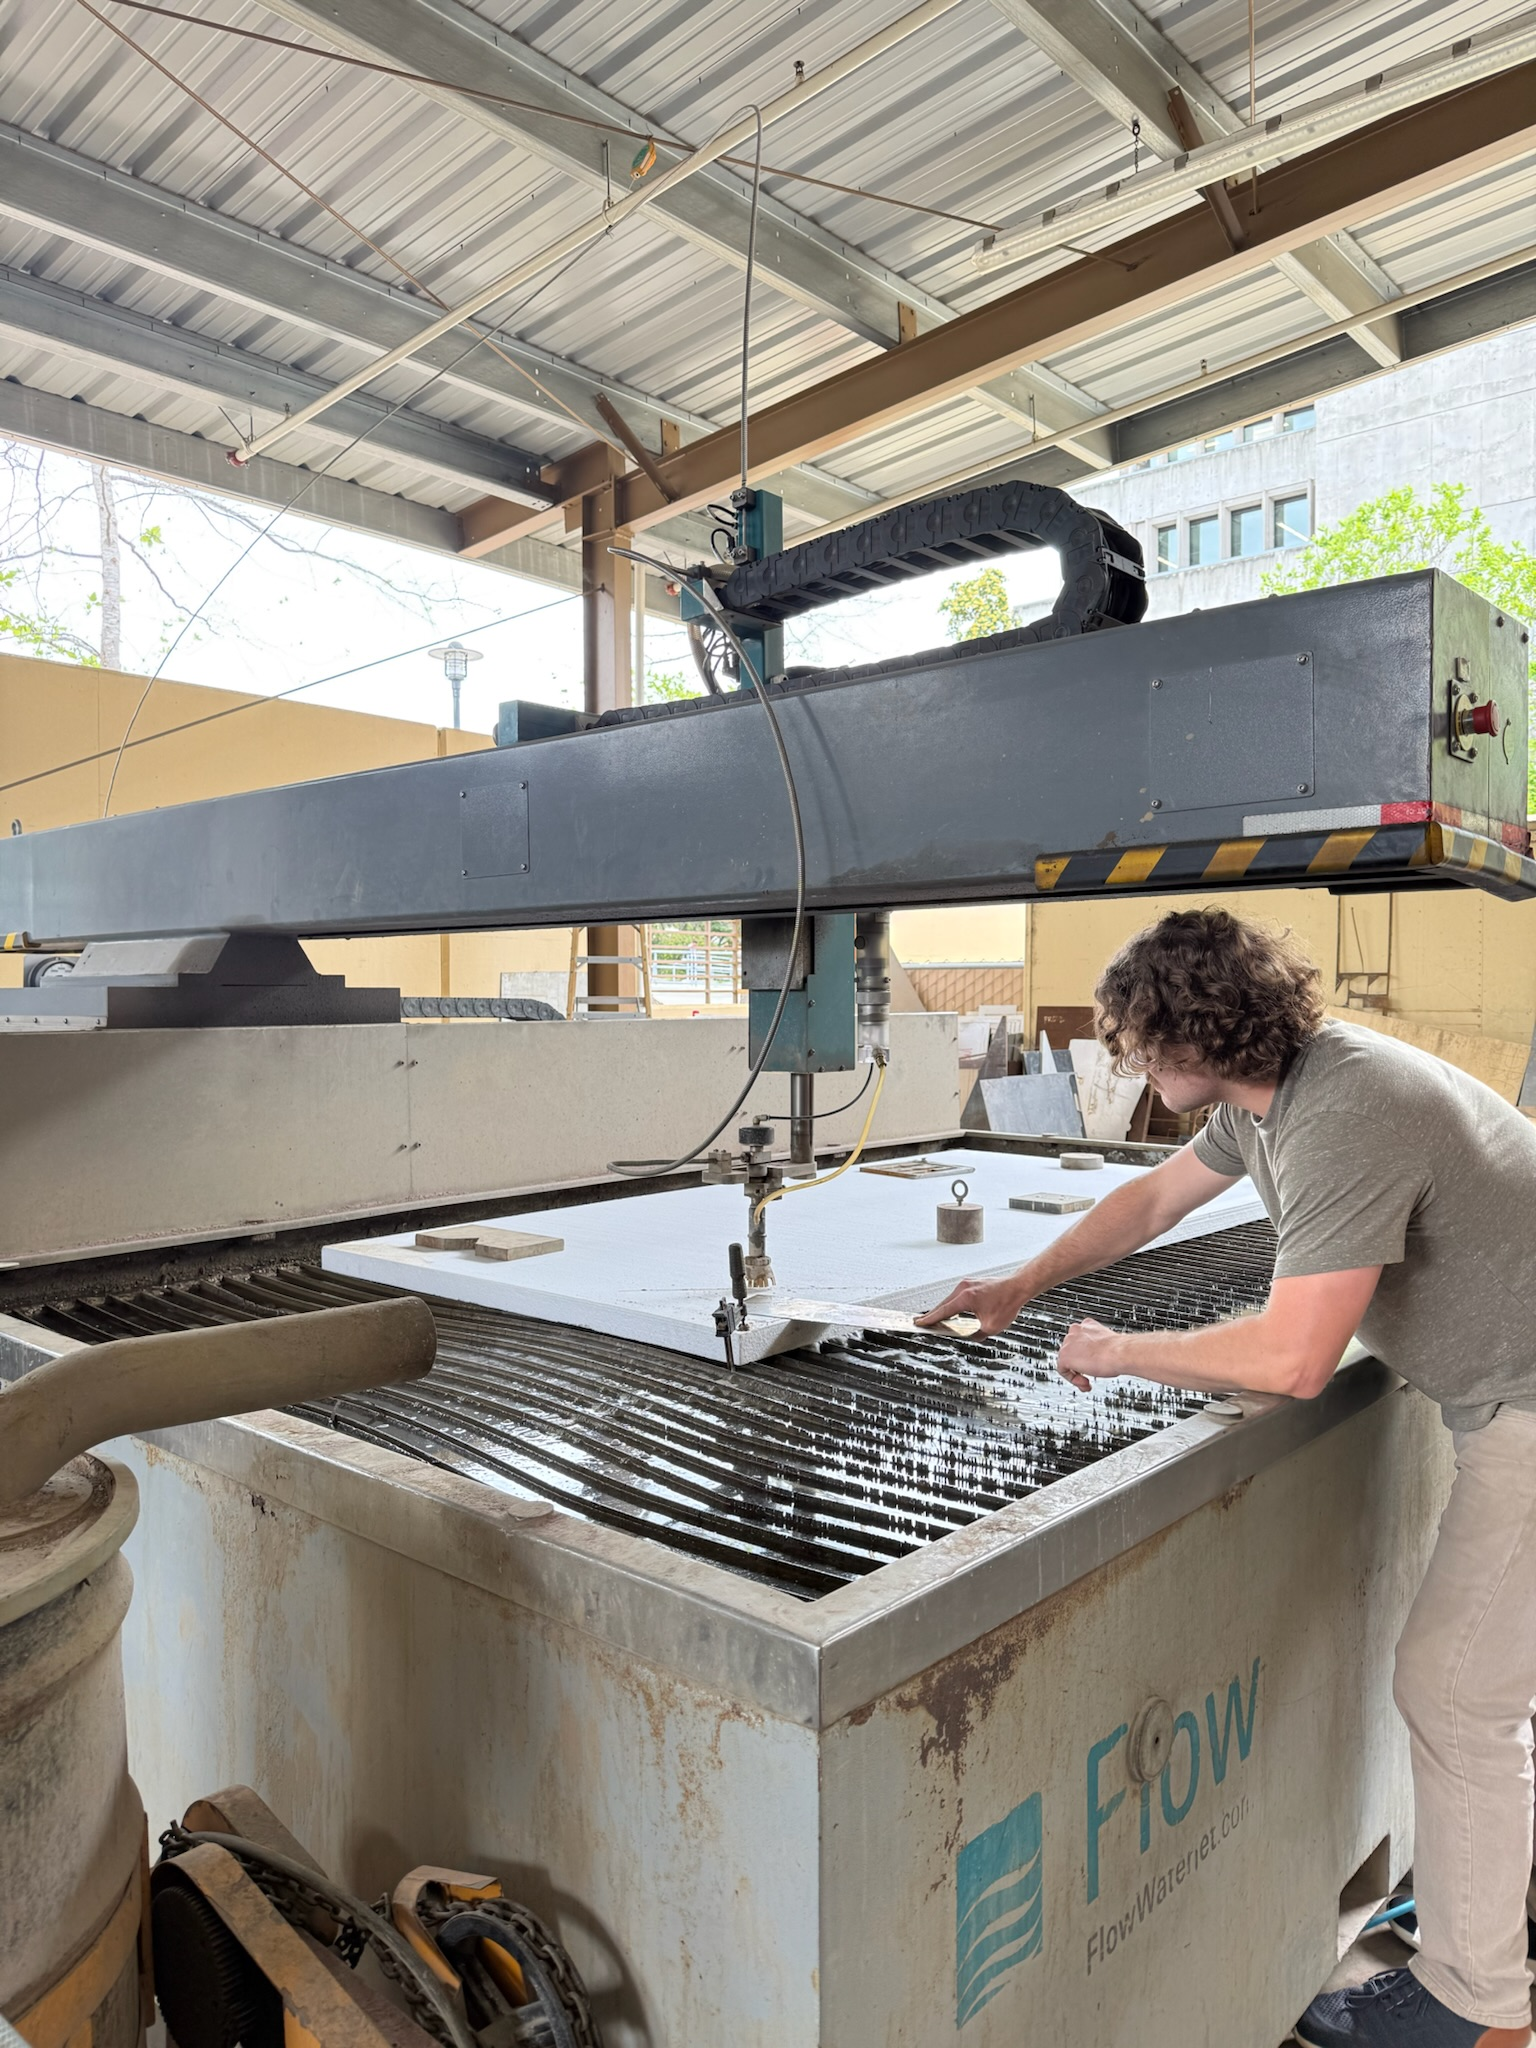
\includegraphics[
        width=3.10in,
        height=1.40in,
        keepaspectratio
    ]{waterjet_foam}
};
\draw[RuleGray,line width=0.55pt,rounded corners=4pt]
    ($(current page.north west)+(0.43in,-3.36in)$)
    rectangle
    ($(current page.north west)+(3.71in,-4.85in)$);

% Row 1 image 2
\node[anchor=center,inner sep=0pt]
at ($(current page.north west)+(5.50in,-4.105in)$)
{
    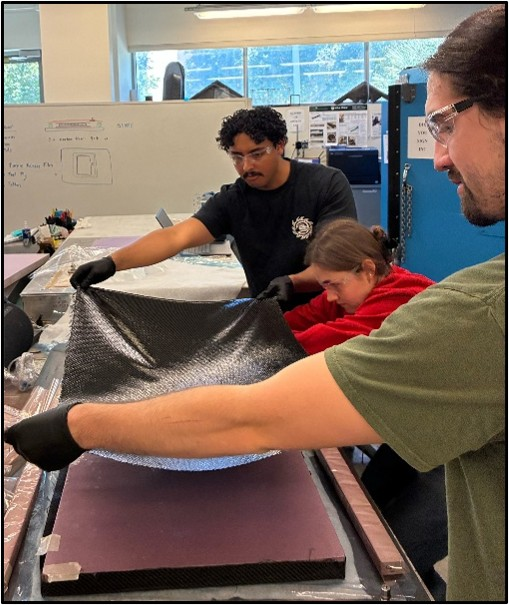
\includegraphics[
        width=3.10in,
        height=1.40in,
        keepaspectratio
    ]{group_layup}
};
\draw[RuleGray,line width=0.55pt,rounded corners=4pt]
    ($(current page.north west)+(3.86in,-3.36in)$)
    rectangle
    ($(current page.north west)+(7.14in,-4.85in)$);

% Row 1 image 3
\node[anchor=center,inner sep=0pt]
at ($(current page.north west)+(8.935in,-4.105in)$)
{
    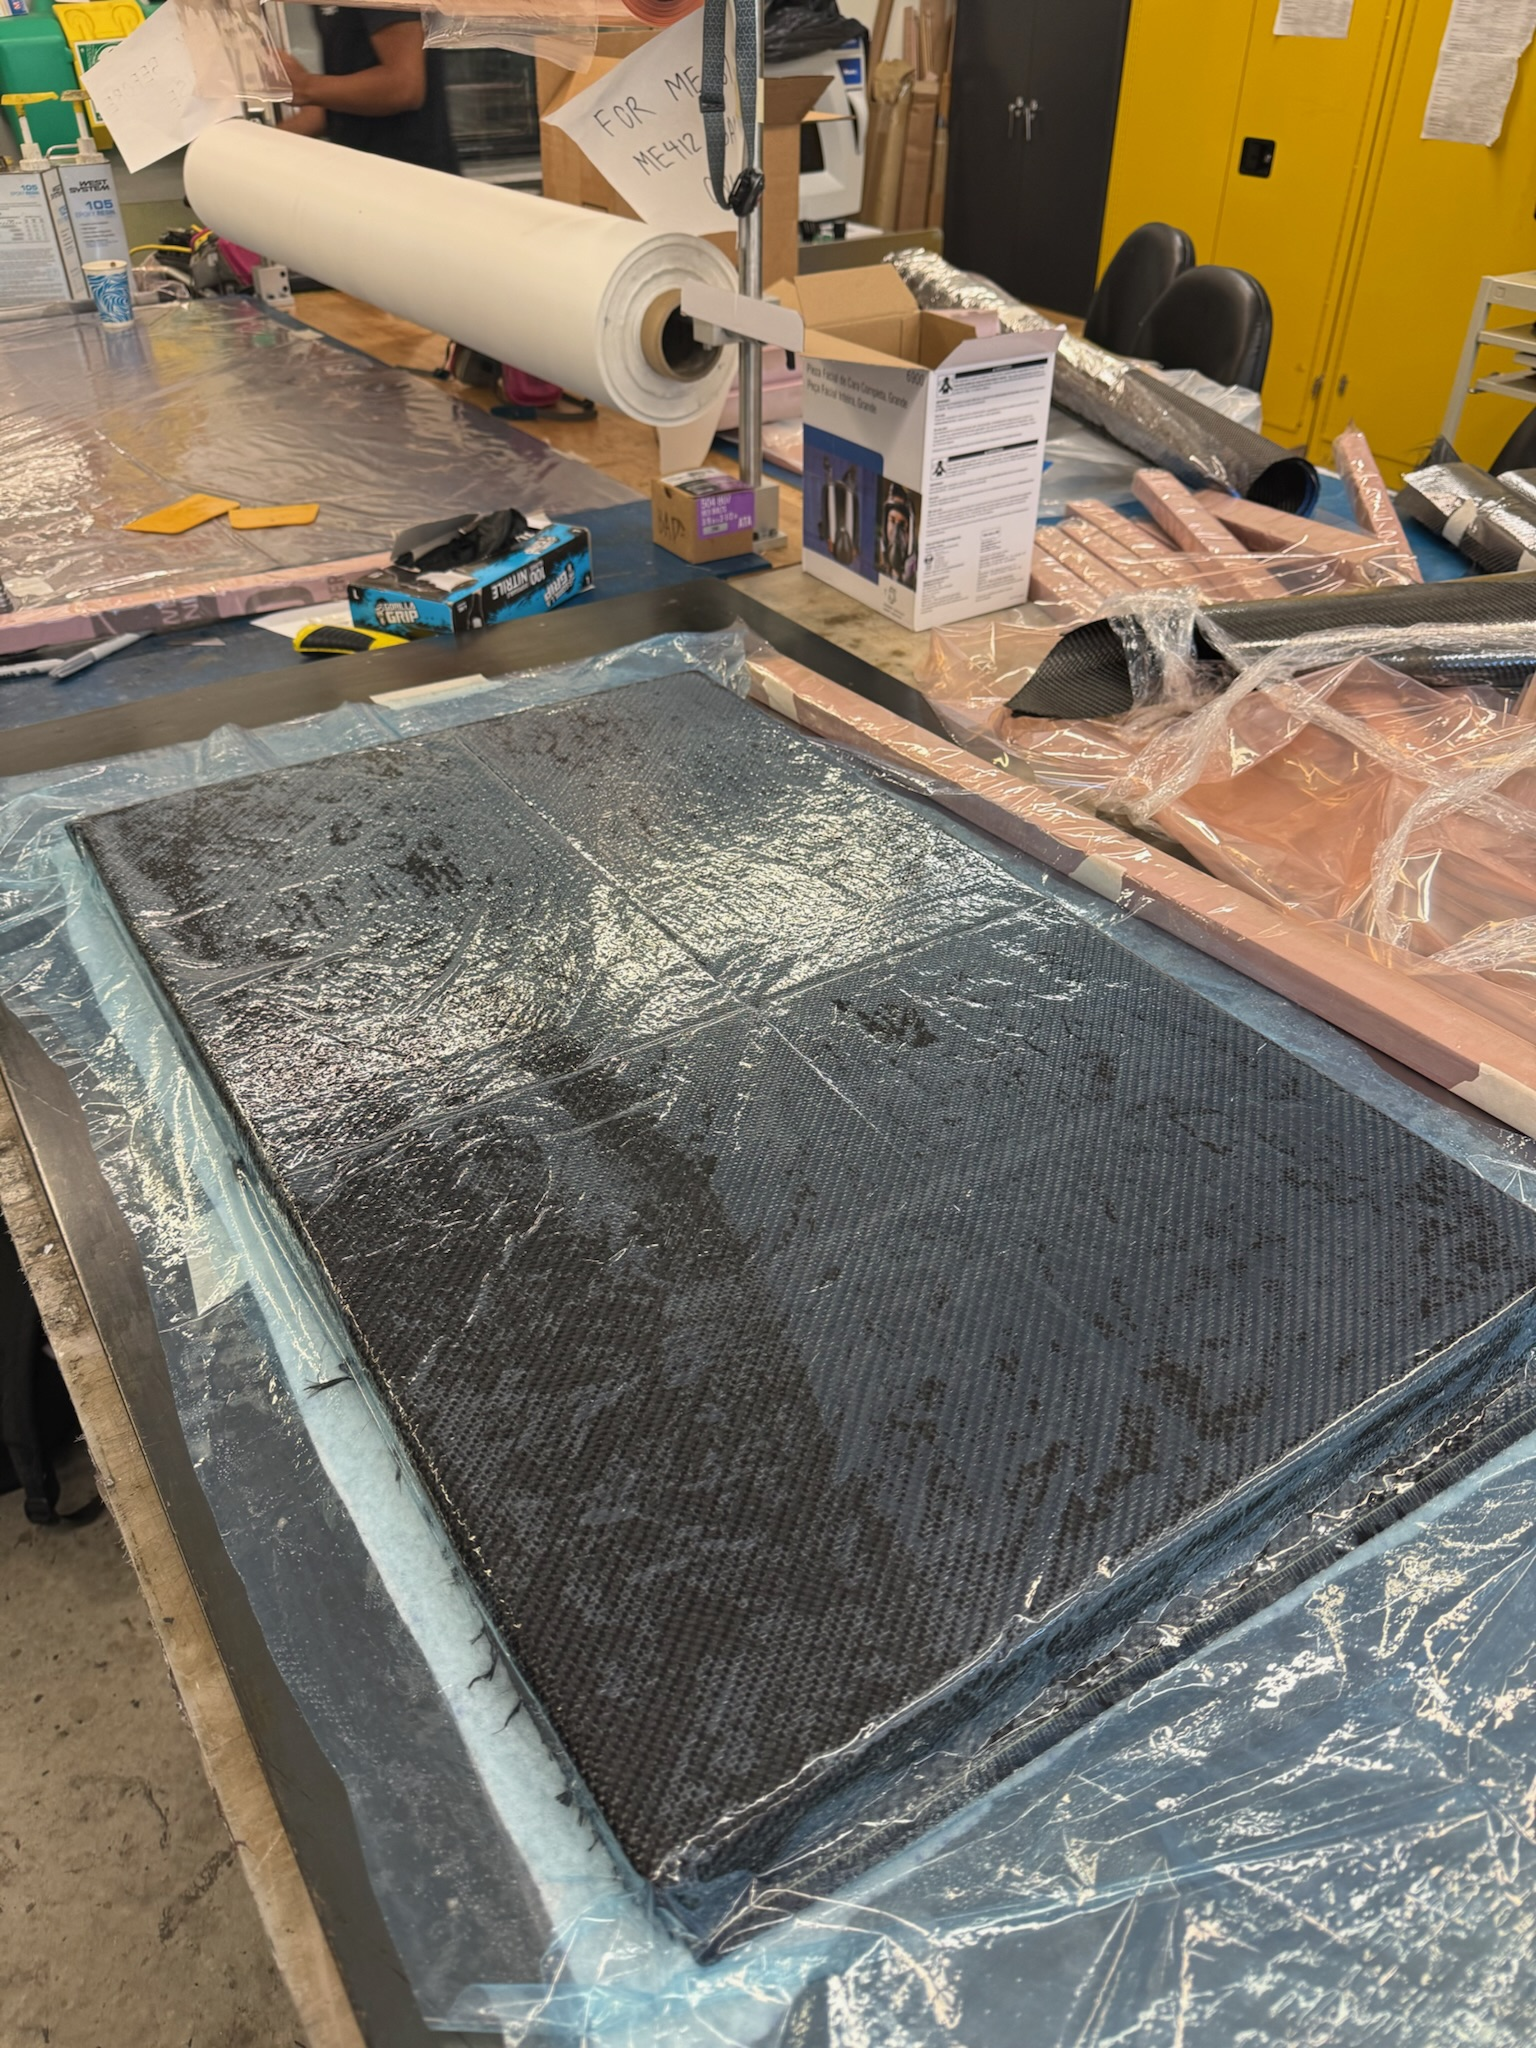
\includegraphics[
        width=3.10in,
        height=1.40in,
        keepaspectratio
    ]{blue_perforrated_film_layup}
};
\draw[RuleGray,line width=0.55pt,rounded corners=4pt]
    ($(current page.north west)+(7.29in,-3.36in)$)
    rectangle
    ($(current page.north east)+(-0.42in,-4.85in)$);

% Row 1 captions
\node[anchor=north,text=Muted,font=\sffamily\fontsize{6.7}{7.3}\selectfont]
at ($(current page.north west)+(2.07in,-4.90in)$)
{1. Waterjet-cut core and perimeter geometry};

\node[anchor=north,text=Muted,font=\sffamily\fontsize{6.7}{7.3}\selectfont]
at ($(current page.north west)+(5.50in,-4.90in)$)
{2. Team wet layup under my process guidance};

\node[anchor=north,text=Muted,font=\sffamily\fontsize{6.7}{7.3}\selectfont]
at ($(current page.north west)+(8.935in,-4.90in)$)
{3. Perforated film, breather, and vacuum enclosure};

% Row 2 image 1
\node[anchor=center,inner sep=0pt]
at ($(current page.north west)+(2.07in,-5.875in)$)
{
    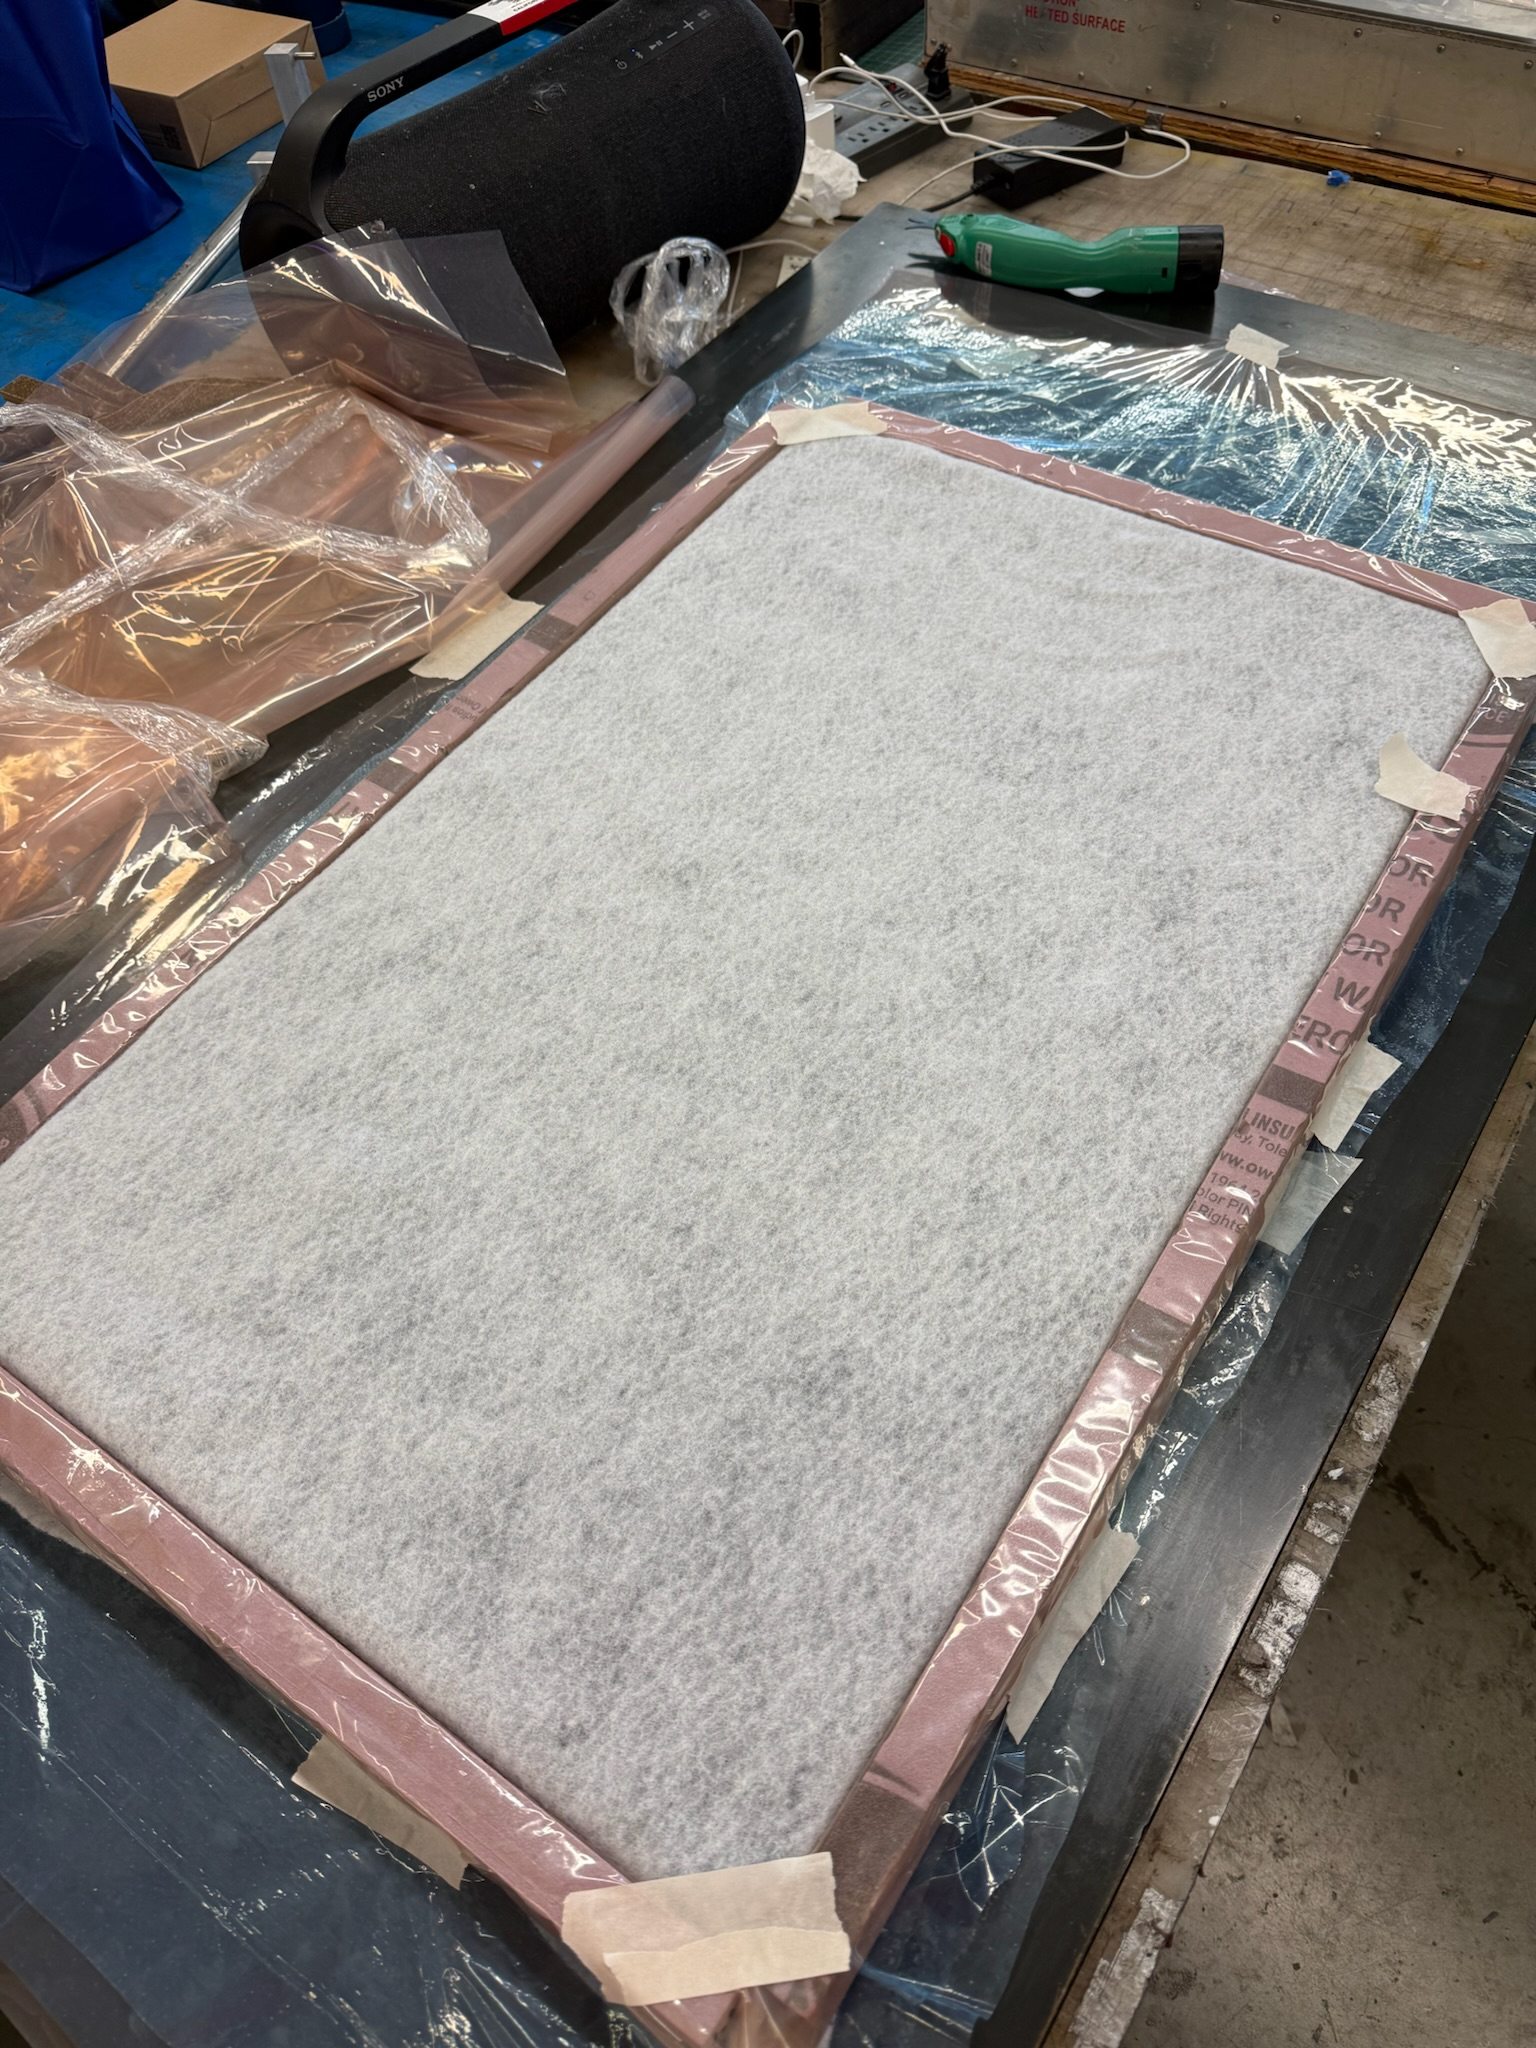
\includegraphics[
        width=3.10in,
        height=1.40in,
        keepaspectratio
    ]{completed_layup}
};
\draw[RuleGray,line width=0.55pt,rounded corners=4pt]
    ($(current page.north west)+(0.43in,-5.13in)$)
    rectangle
    ($(current page.north west)+(3.71in,-6.62in)$);

% Row 2 image 2 — oven chamber used only as a reliable vacuum enclosure; no heat applied
\node[anchor=center,inner sep=0pt]
at ($(current page.north west)+(5.50in,-5.875in)$)
{
    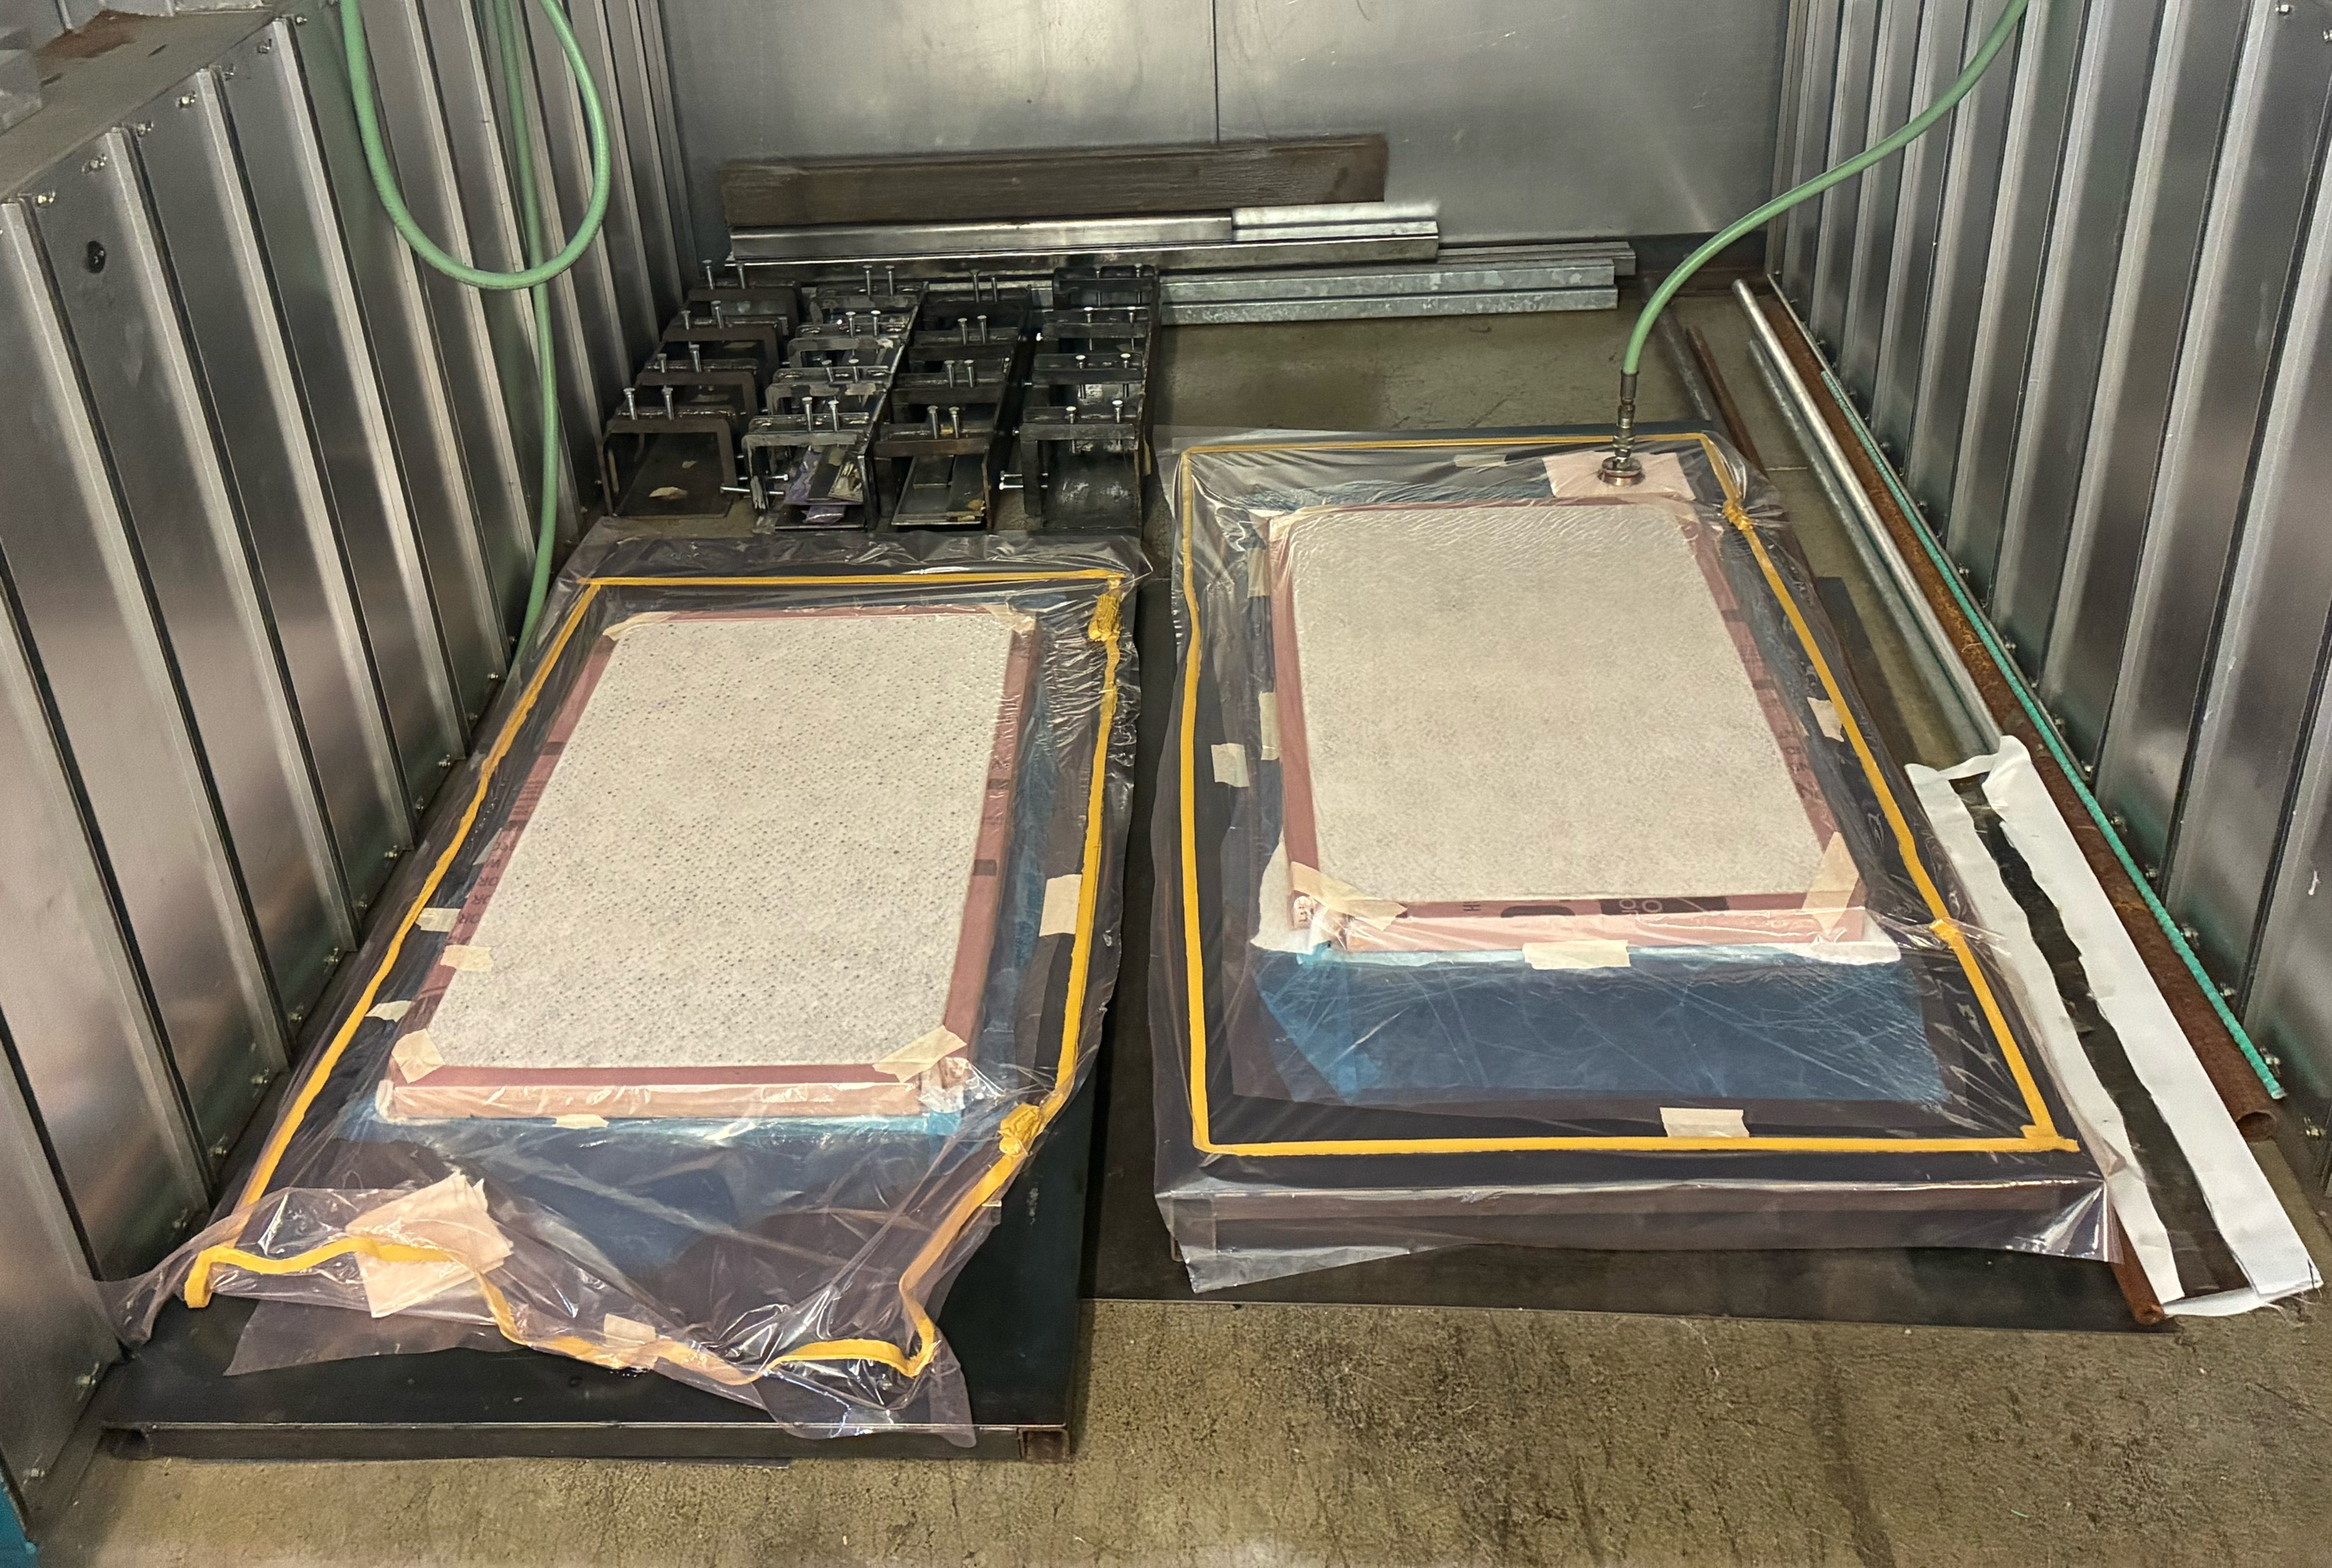
\includegraphics[
        width=3.10in,
        height=1.40in,
        keepaspectratio
    ]{layups_in_composite_oven_under_vacuumPressure}
};
\draw[RuleGray,line width=0.55pt,rounded corners=4pt]
    ($(current page.north west)+(3.86in,-5.13in)$)
    rectangle
    ($(current page.north west)+(7.14in,-6.62in)$);

% Row 2 image 3
\node[anchor=center,inner sep=0pt]
at ($(current page.north west)+(8.935in,-5.875in)$)
{
    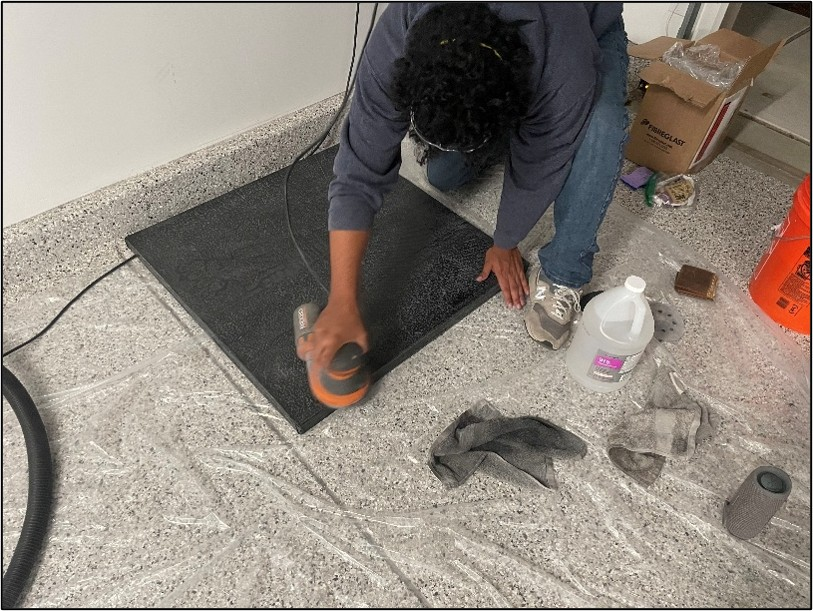
\includegraphics[
        width=3.10in,
        height=1.40in,
        keepaspectratio
    ]{garage_sanding}
};
\draw[RuleGray,line width=0.55pt,rounded corners=4pt]
    ($(current page.north west)+(7.29in,-5.13in)$)
    rectangle
    ($(current page.north east)+(-0.42in,-6.62in)$);

% Row 2 captions
\node[anchor=north,text=Muted,font=\sffamily\fontsize{6.7}{7.3}\selectfont]
at ($(current page.north west)+(2.07in,-6.67in)$)
{4. Fully saturated carbon skin and foam sandwich};

\node[anchor=north,text=Muted,font=\sffamily\fontsize{6.7}{7.3}\selectfont]
at ($(current page.north west)+(5.50in,-6.67in)$)
{5. Room-temperature cure under continuous vacuum};

\node[anchor=north,text=Muted,font=\sffamily\fontsize{6.7}{7.3}\selectfont]
at ($(current page.north west)+(8.935in,-6.67in)$)
{6. Post-processing and surface preparation};

% Bottom callouts
\fill[Panel,rounded corners=4pt]
    ($(current page.north west)+(0.43in,-6.95in)$)
    rectangle
    ($(current page.north west)+(5.48in,-7.60in)$);

\draw[RuleGray,line width=0.55pt,rounded corners=4pt]
    ($(current page.north west)+(0.43in,-6.95in)$)
    rectangle
    ($(current page.north west)+(5.48in,-7.60in)$);

\node[
    anchor=north west,
    text=DeepGreen,
    font=\sffamily\bfseries\fontsize{7.0}{7.6}\selectfont
]
at ($(current page.north west)+(0.63in,-7.08in)$)
{FROM THREE LAYUPS TO ONE};

\node[
    anchor=north west,
    align=left,
    text width=4.56in,
    text=Ink,
    font=\fontsize{6.45}{7.45}\selectfont
]
at ($(current page.north west)+(0.63in,-7.29in)$)
{
The Envelope Method reduced labor, cure cycles, handling,
alignment risk, and time spent forming numerous vacuum-bag
pleats around the 1.5-inch-thick XPS panels.
};

\fill[Panel,rounded corners=4pt]
    ($(current page.north west)+(5.68in,-6.95in)$)
    rectangle
    ($(current page.north east)+(-0.42in,-7.60in)$);

\draw[RuleGray,line width=0.55pt,rounded corners=4pt]
    ($(current page.north west)+(5.68in,-6.95in)$)
    rectangle
    ($(current page.north east)+(-0.42in,-7.60in)$);

\node[
    anchor=north west,
    text=DeepGreen,
    font=\sffamily\bfseries\fontsize{7.0}{7.6}\selectfont
]
at ($(current page.north west)+(5.88in,-7.08in)$)
{WHY SURFACE-BONDED HARDWARE};

\node[
    anchor=north west,
    align=left,
    text width=4.55in,
    text=Ink,
    font=\fontsize{6.45}{7.45}\selectfont
]
at ($(current page.north west)+(5.88in,-7.29in)$)
{
Adhesively bonded hinges and fixtures preserved the clean
composite exterior and avoided drilled inserts, foam-core
crushing, added stress concentrations, and new leak paths.
};


% Footer
\node[
    anchor=south west,
    text=white,
    font=\sffamily\bfseries\fontsize{7.1}{7.7}\selectfont
]
at ($(current page.south west)+(0.42in,0.17in)$)
{\faArrowLeft\ PRODUCT ARCHITECTURE};

\node[
    anchor=south,
    text=white,
    font=\sffamily\fontsize{7.0}{7.6}\selectfont
]
at ($(current page.south)+(0,0.17in)$)
{TORO COVER \hspace{6pt} 2 / 3};

\node[
    anchor=south east,
    text=white,
    font=\sffamily\bfseries\fontsize{7.1}{7.7}\selectfont
]
at ($(current page.south east)+(-0.42in,0.17in)$)
{VALIDATION \& TAKEAWAYS \faArrowRight};

\end{tikzpicture}


% ============================================================
% PAGE 3 — FINISHING, VALIDATION, AND TAKEAWAYS
% ============================================================

\clearpage
\thispagestyle{empty}
\hypertarget{toro-results}{}
\null

\begin{tikzpicture}[remember picture,overlay]

% Background and bars
\fill[white]
    (current page.south west)
    rectangle
    (current page.north east);

\fill[DeepGreen]
    (current page.north west)
    rectangle
    ($(current page.north east)+(0,-0.095in)$);

\fill[PolyGold]
    ($(current page.north west)+(0,-0.095in)$)
    rectangle
    ($(current page.north east)+(0,-0.14in)$);

\fill[DeepGreen]
    (current page.south west)
    rectangle
    ($(current page.south east)+(0,0.36in)$);

\fill[PolyGold]
    ($(current page.south west)+(0,0.36in)$)
    rectangle
    ($(current page.south east)+(0,0.405in)$);

% Header
\node[
    anchor=north west,
    text=PolyGold,
    font=\sffamily\bfseries\fontsize{8.1}{8.7}\selectfont
]
at ($(current page.north west)+(0.42in,-0.39in)$)
{TORO COVER \hspace{5pt}/\hspace{5pt} VALIDATION AND ENGINEERING TAKEAWAYS};

\node[
    anchor=north west,
    text=DeepGreen,
    font=\bfseries\fontsize{22.5}{23.5}\selectfont
]
at ($(current page.north west)+(0.40in,-0.67in)$)
{FROM PROTOTYPE TO PRODUCT PATHWAY};

\node[
    anchor=north west,
    text=Muted,
    font=\sffamily\fontsize{8.7}{9.6}\selectfont
]
at ($(current page.north west)+(0.42in,-1.12in)$)
{Environmental protection, usability testing, scope decisions, and lessons from technical leadership};

\fill[PolyGold]
    ($(current page.north west)+(0.42in,-1.36in)$)
    rectangle
    ($(current page.north west)+(5.8in,-1.315in)$);

% Finishing title
\node[
    anchor=north west,
    text=DeepGreen,
    font=\sffamily\bfseries\fontsize{8.0}{8.7}\selectfont
]
at ($(current page.north west)+(0.43in,-1.62in)$)
{OUTDOOR FINISHING AND ENVIRONMENTAL PROTECTION};

% Image 1
\node[anchor=center,inner sep=0pt]
at ($(current page.north west)+(1.705in,-2.655in)$)
{
    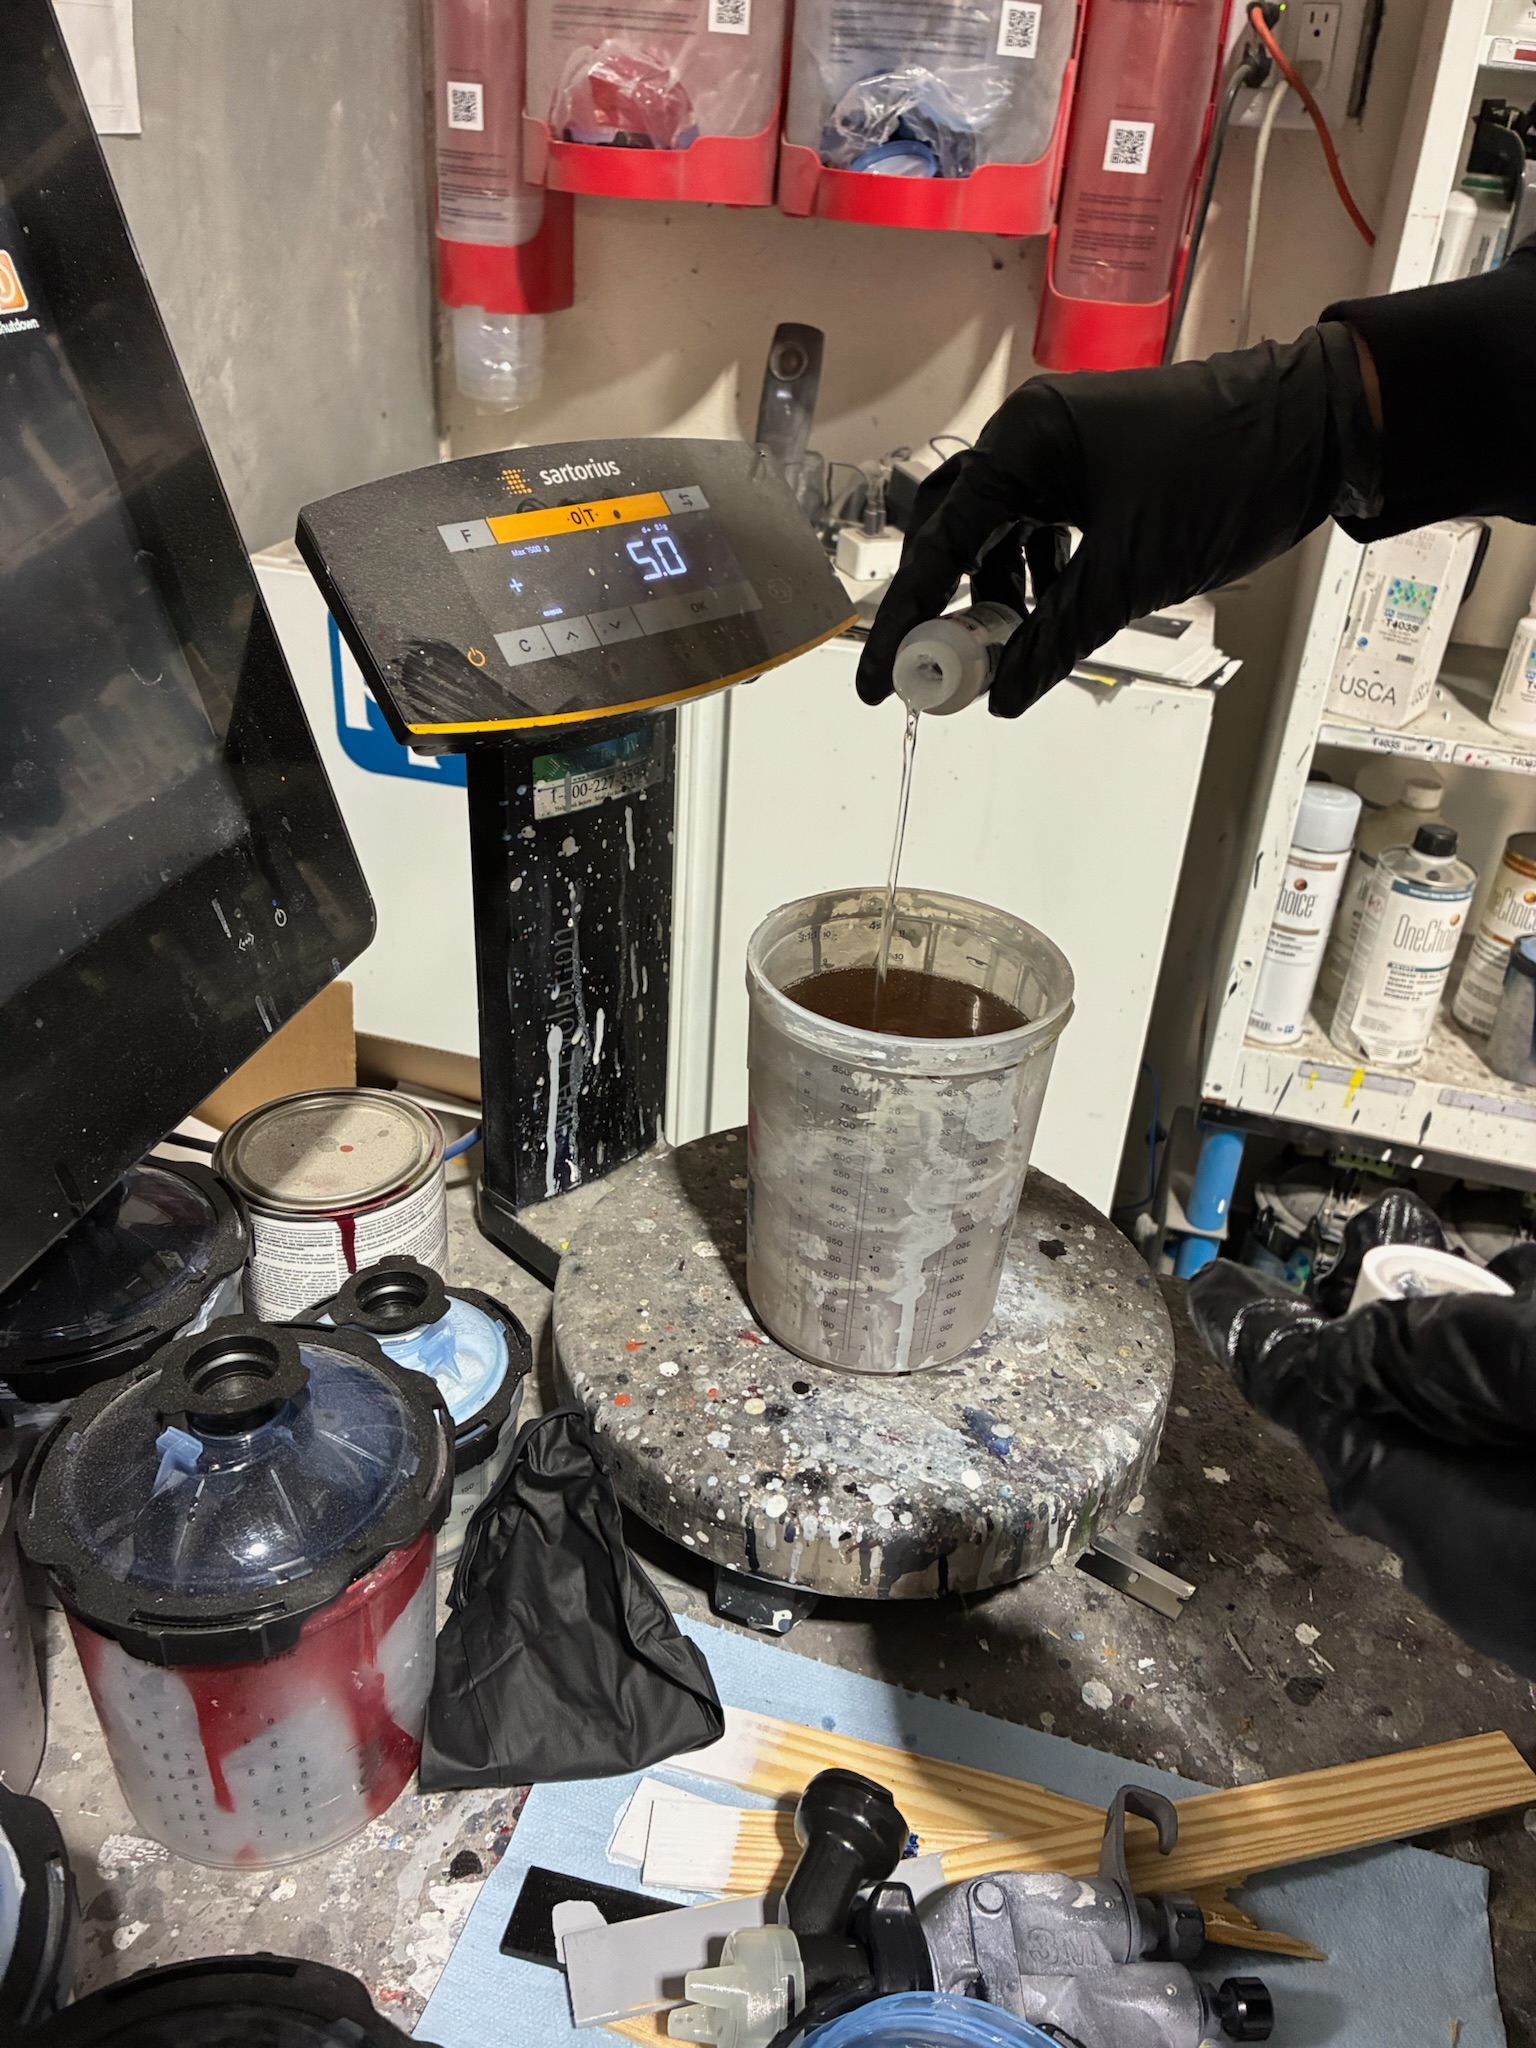
\includegraphics[
        width=2.35in,
        height=1.40in,
        keepaspectratio
    ]{spray_topcoat_prep}
};
\draw[RuleGray,line width=0.55pt,rounded corners=4pt]
    ($(current page.north west)+(0.43in,-1.91in)$)
    rectangle
    ($(current page.north west)+(2.98in,-3.40in)$);

% Image 2
\node[anchor=center,inner sep=0pt]
at ($(current page.north west)+(4.375in,-2.655in)$)
{
    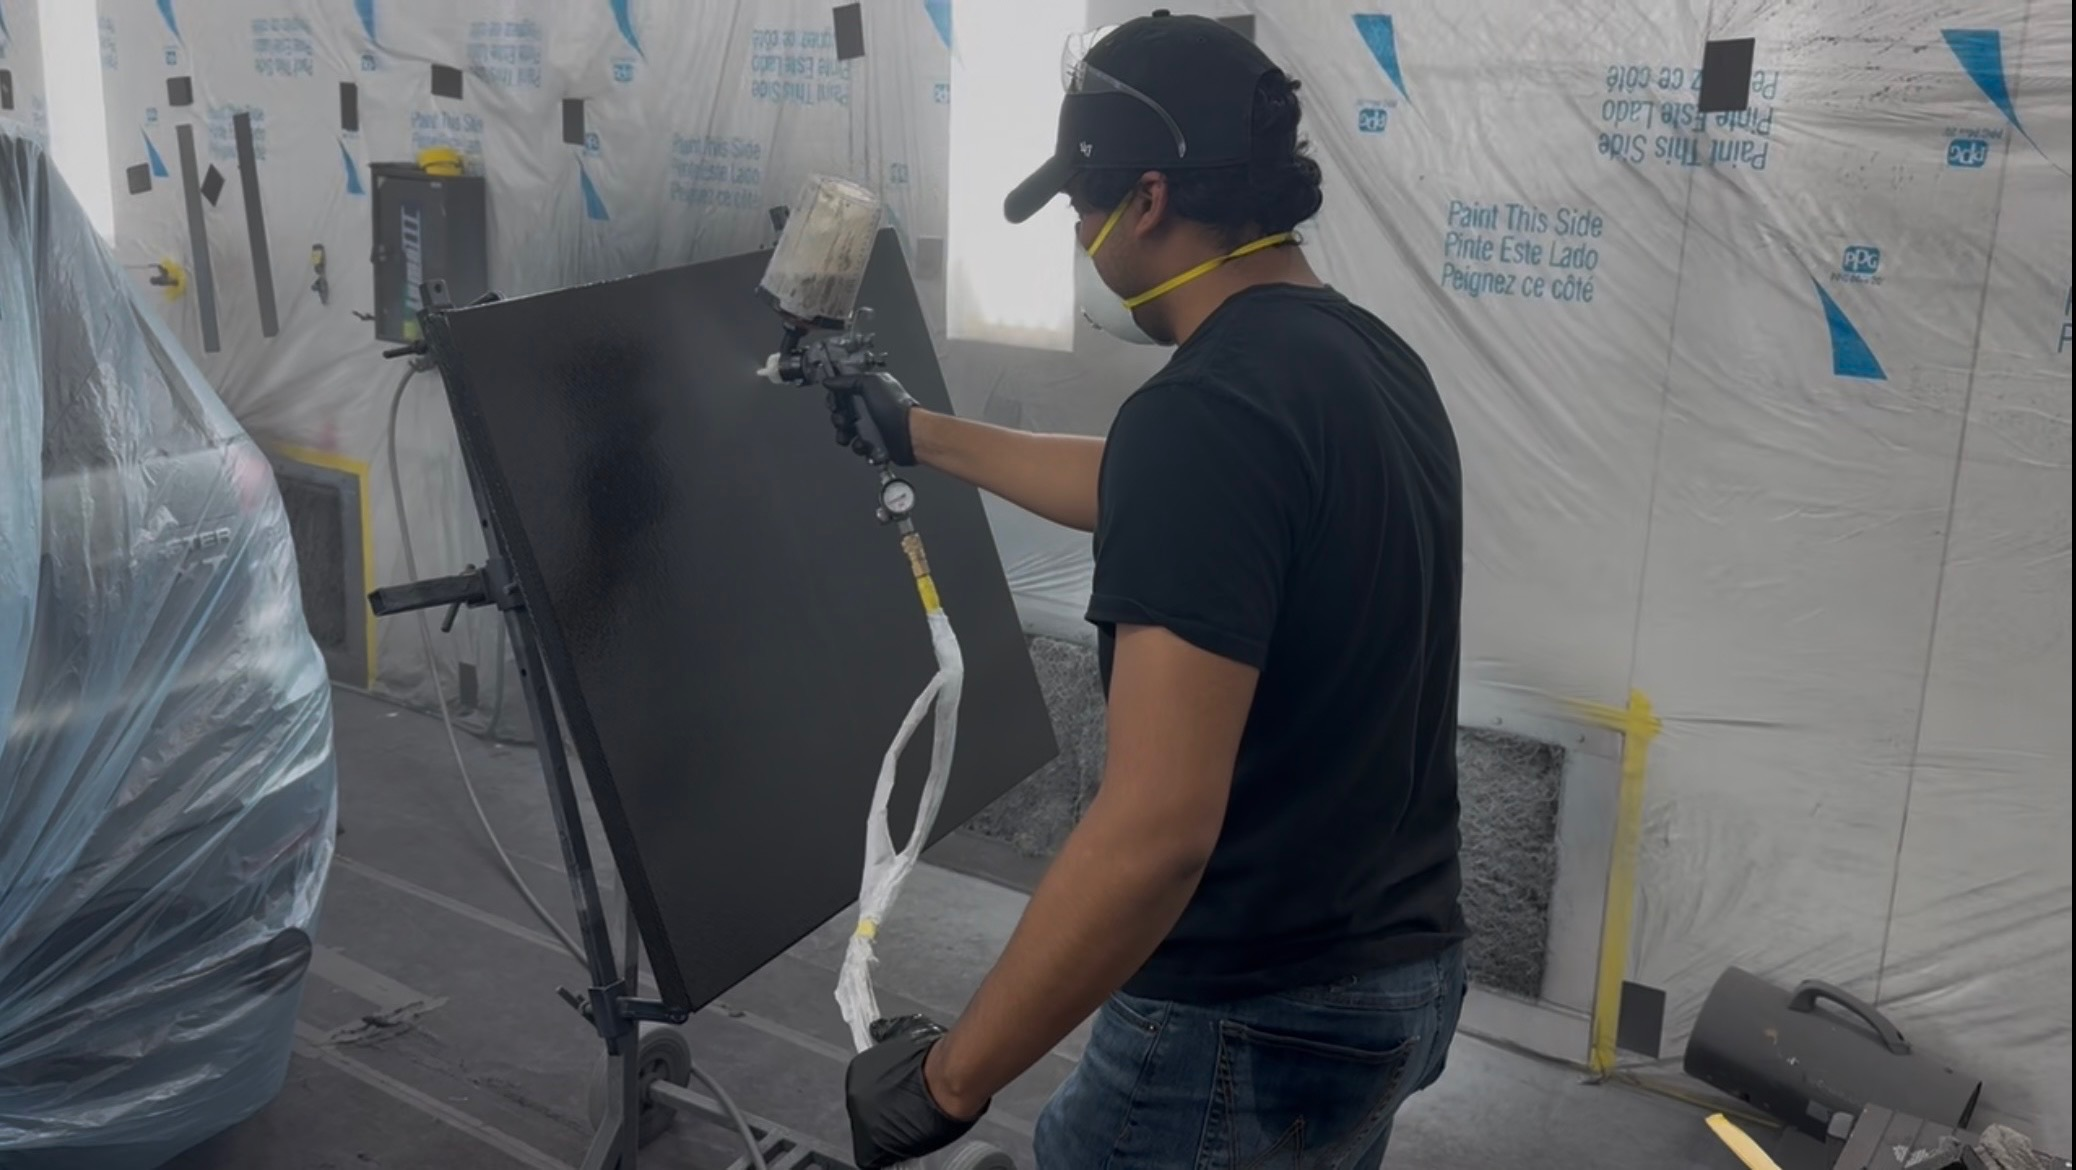
\includegraphics[
        width=2.35in,
        height=1.40in,
        keepaspectratio
    ]{spraying_topcoat}
};
\draw[RuleGray,line width=0.55pt,rounded corners=4pt]
    ($(current page.north west)+(3.10in,-1.91in)$)
    rectangle
    ($(current page.north west)+(5.65in,-3.40in)$);

% Image 3
\node[anchor=center,inner sep=0pt]
at ($(current page.north west)+(7.045in,-2.655in)$)
{
    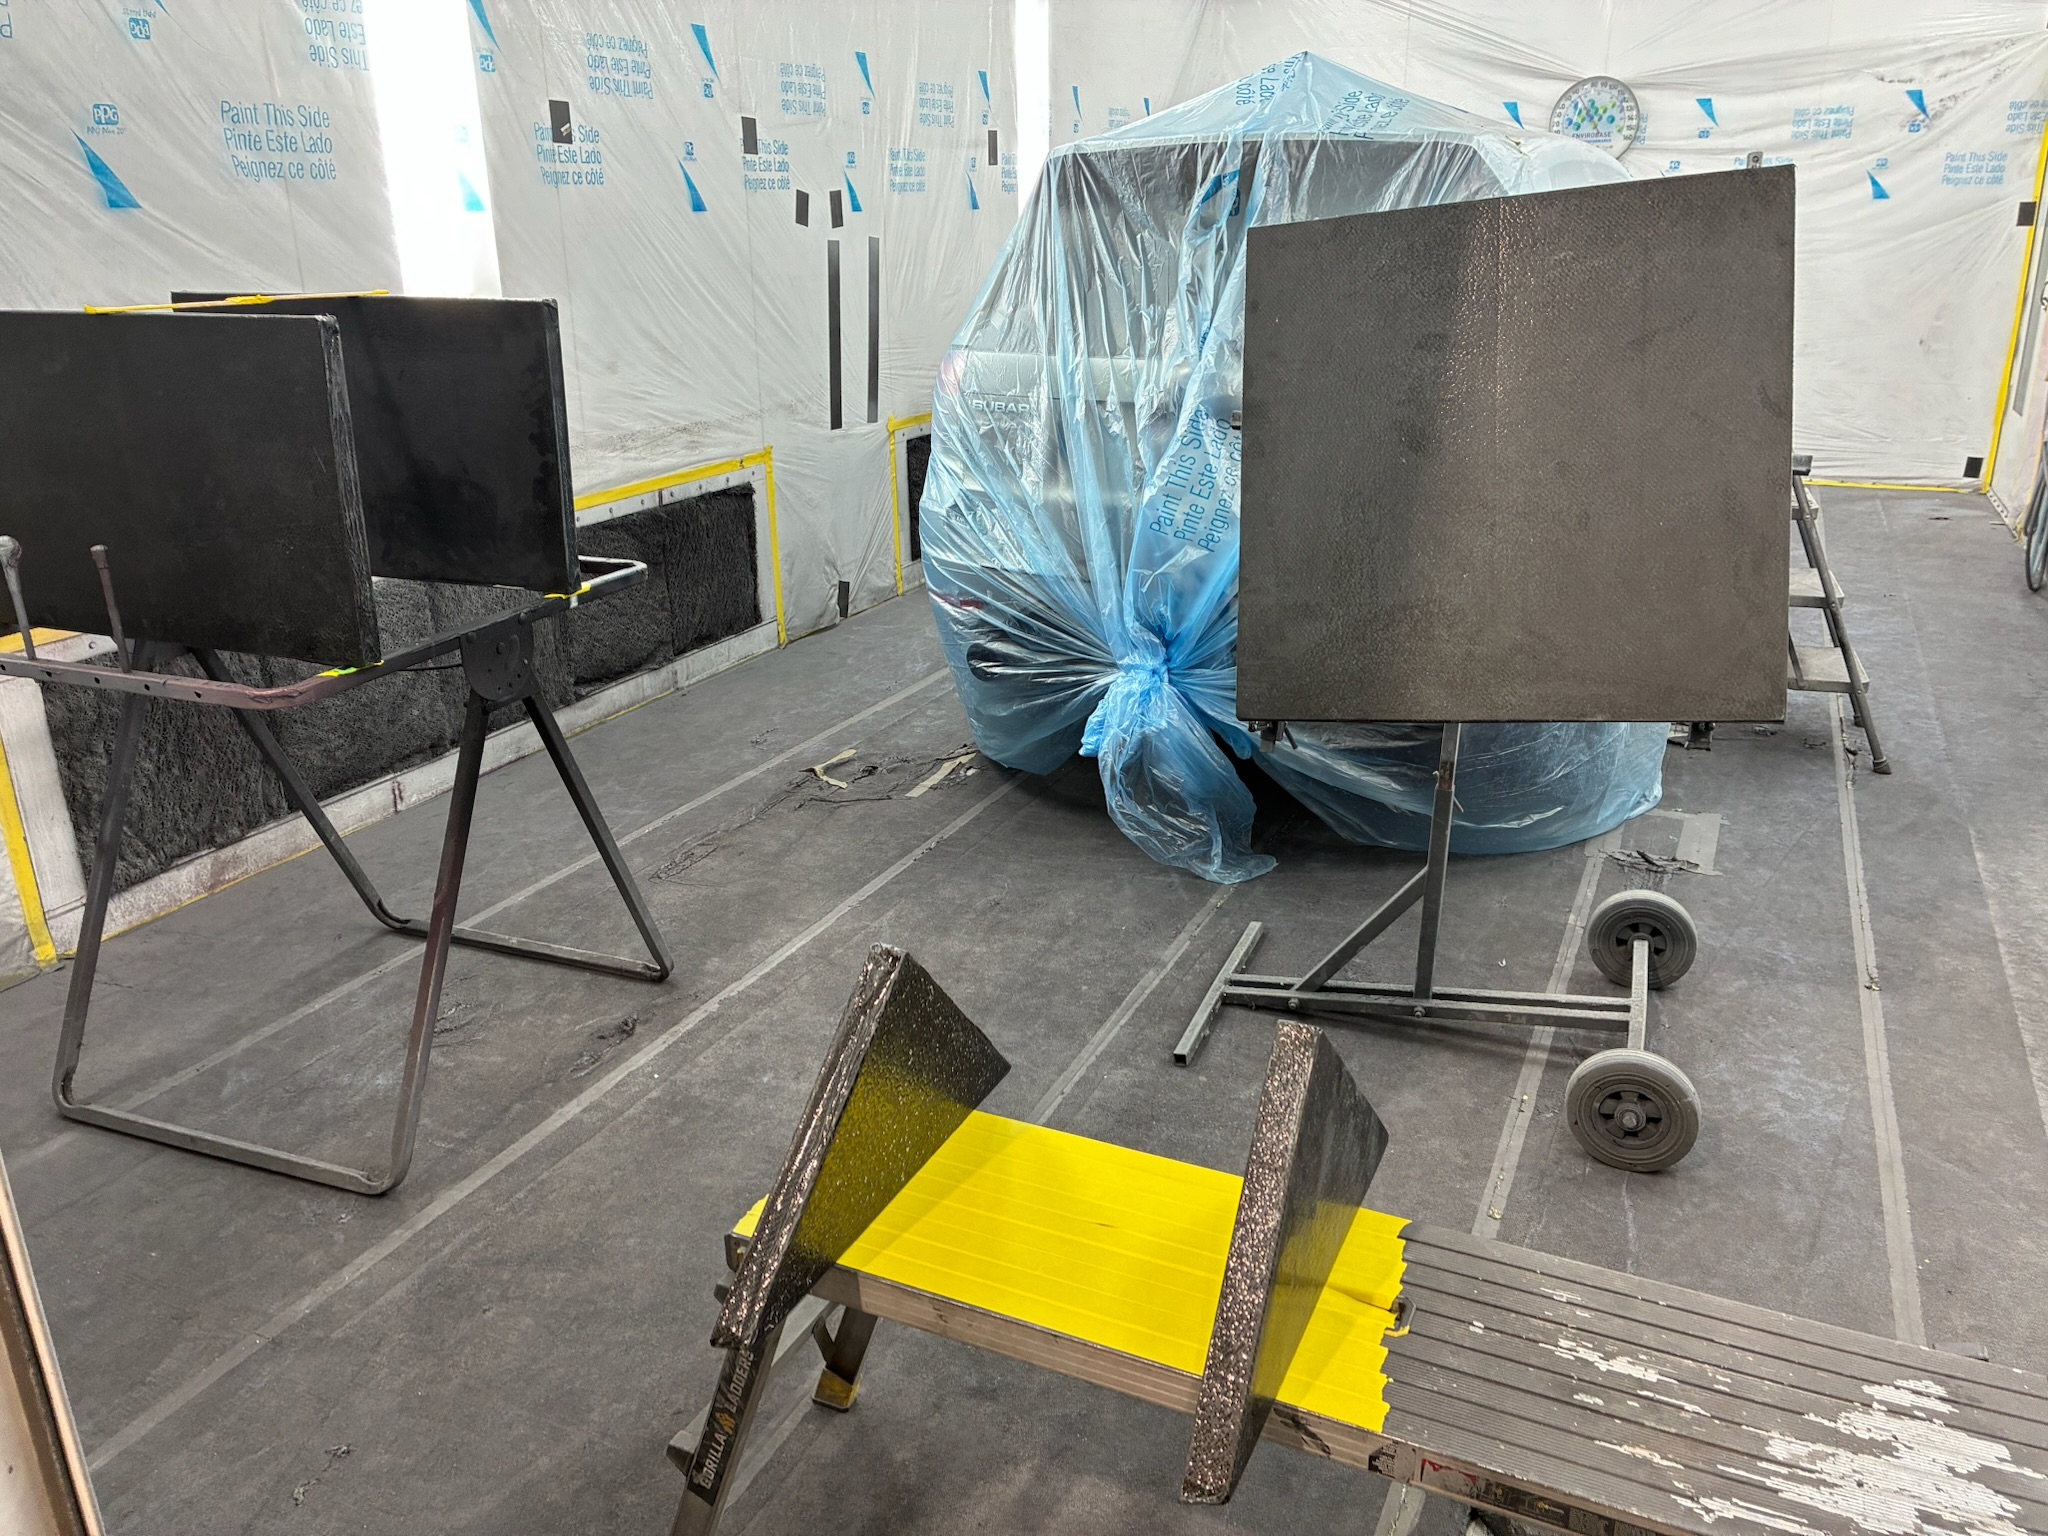
\includegraphics[
        width=2.35in,
        height=1.40in,
        keepaspectratio
    ]{topcoat_setup_apparatus}
};
\draw[RuleGray,line width=0.55pt,rounded corners=4pt]
    ($(current page.north west)+(5.77in,-1.91in)$)
    rectangle
    ($(current page.north west)+(8.32in,-3.40in)$);

% Image 4
\node[anchor=center,inner sep=0pt]
at ($(current page.north west)+(9.50in,-2.655in)$)
{
    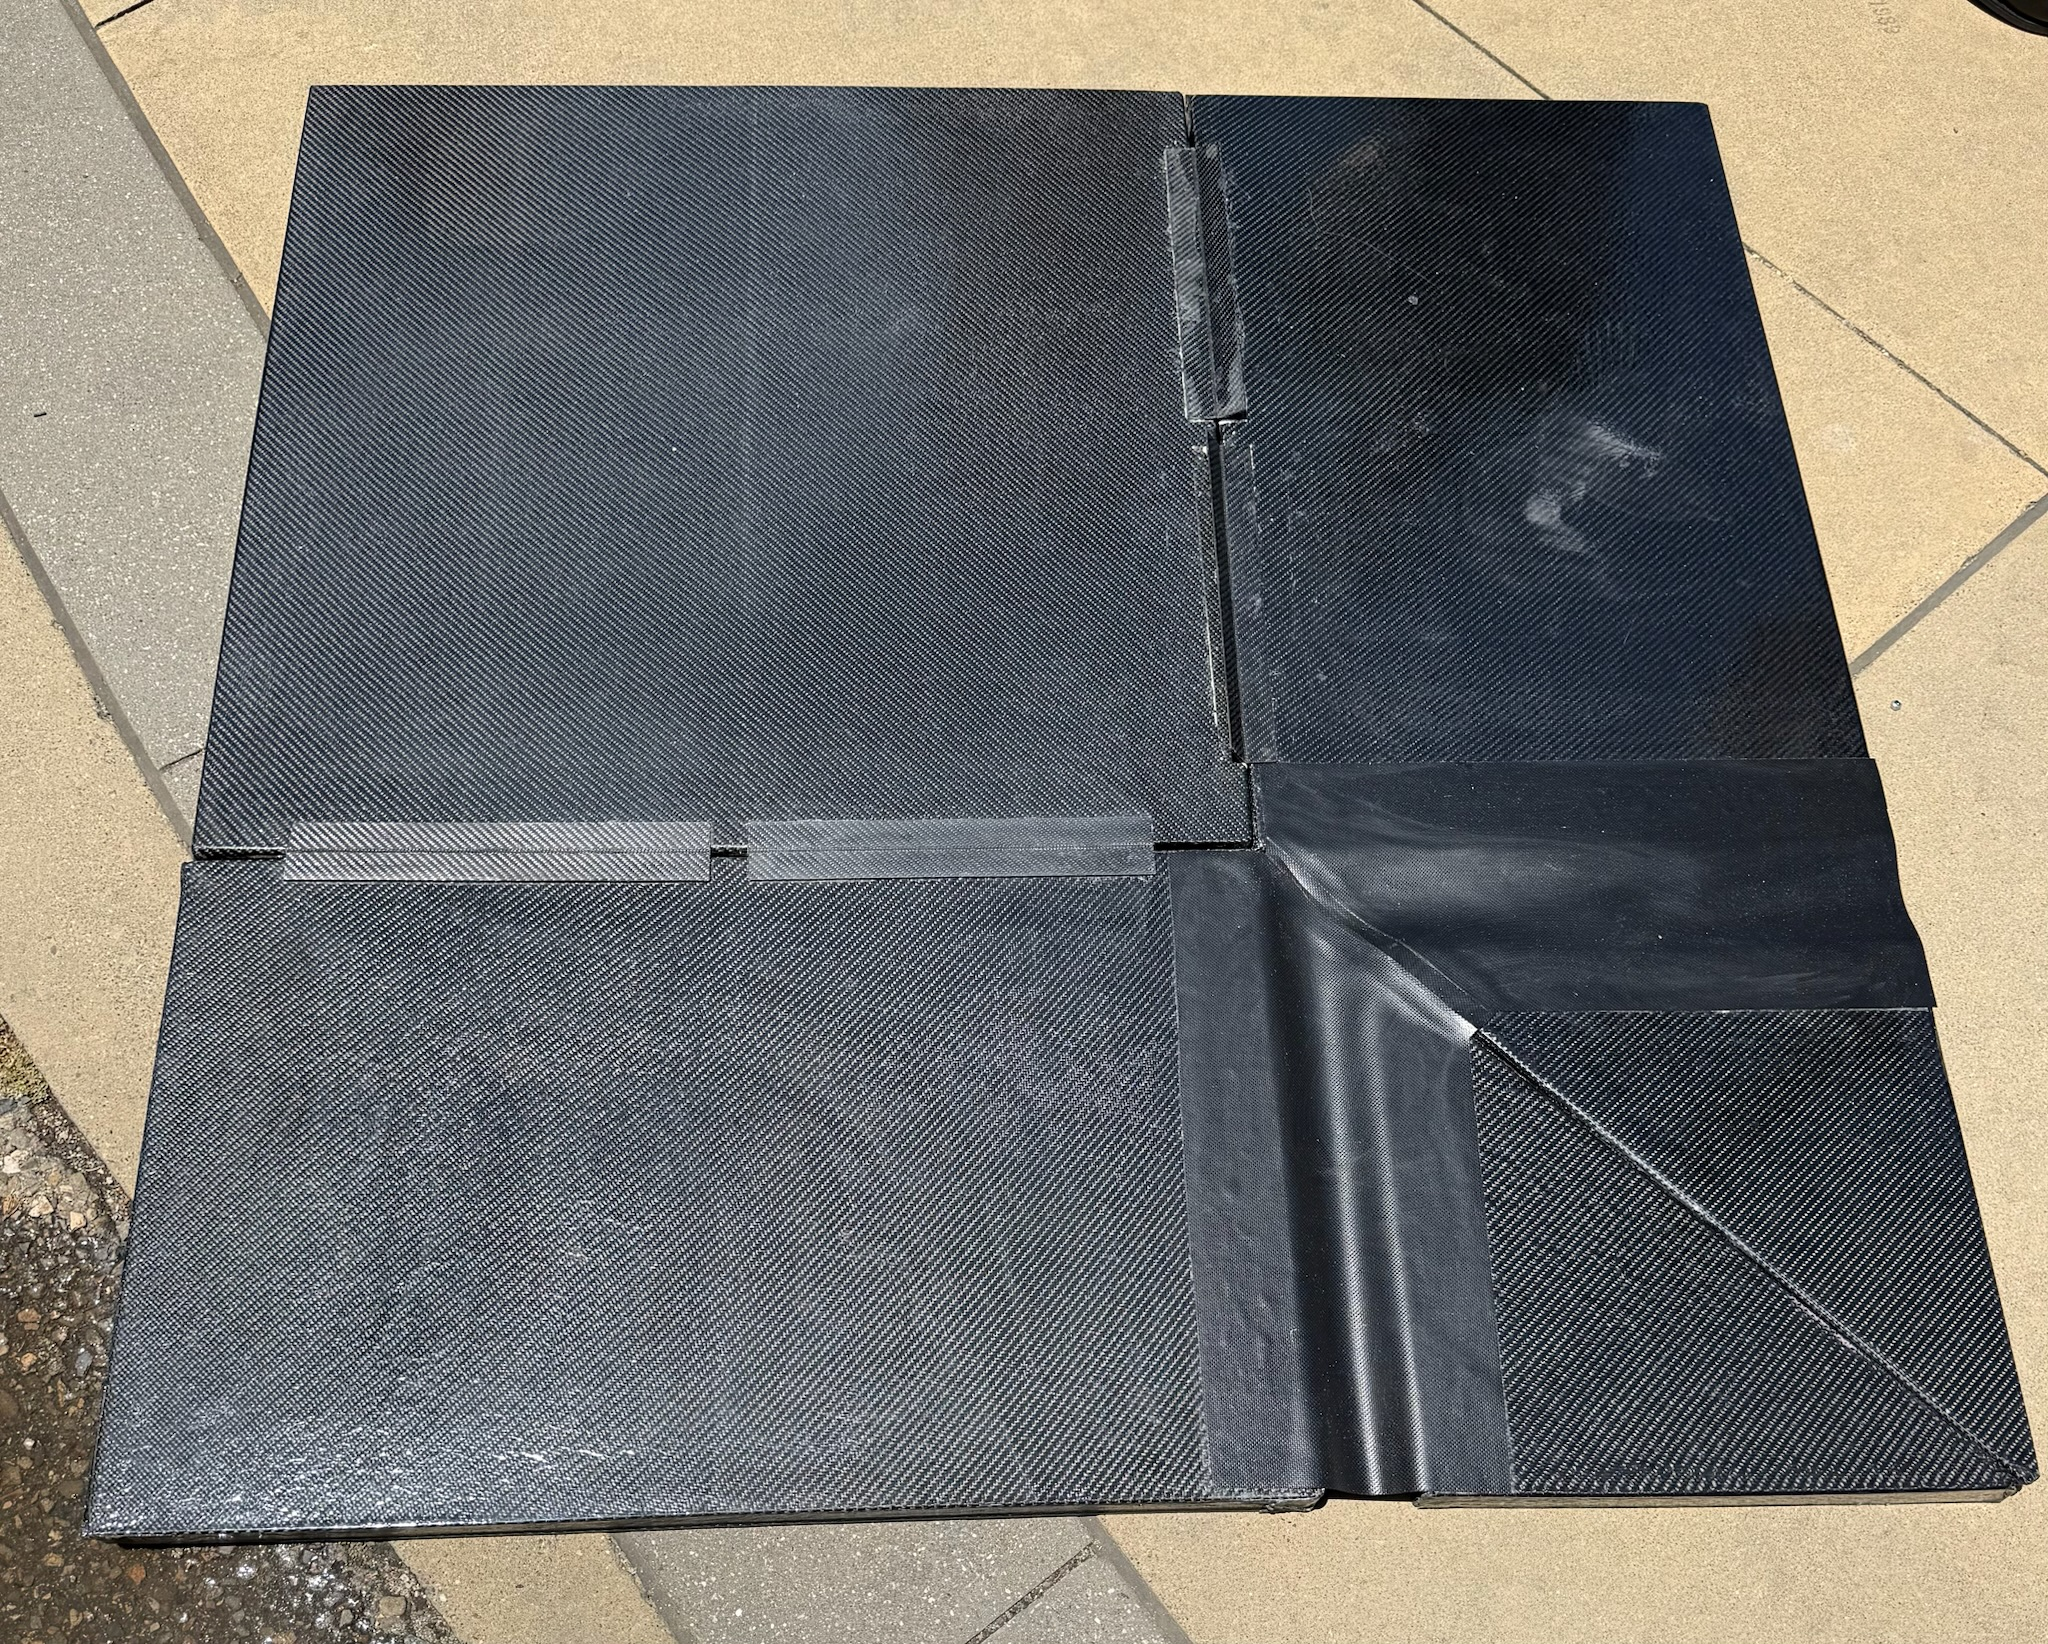
\includegraphics[
        width=2.35in,
        height=1.40in,
        keepaspectratio
    ]{refined_final_toro_cover_partial_carbon_model}
};
\draw[RuleGray,line width=0.55pt,rounded corners=4pt]
    ($(current page.north west)+(8.44in,-1.91in)$)
    rectangle
    ($(current page.north east)+(-0.42in,-3.40in)$);

% Captions
\node[anchor=north,text=Muted,font=\sffamily\fontsize{6.7}{7.3}\selectfont]
at ($(current page.north west)+(1.705in,-3.45in)$)
{Topcoat material preparation};

\node[anchor=north,text=Muted,font=\sffamily\fontsize{6.7}{7.3}\selectfont]
at ($(current page.north west)+(4.375in,-3.45in)$)
{Automotive-booth topcoat application};

\node[anchor=north,text=Muted,font=\sffamily\fontsize{6.7}{7.3}\selectfont]
at ($(current page.north west)+(7.045in,-3.45in)$)
{Coated panels drying after application};

\node[anchor=north,text=Muted,font=\sffamily\fontsize{6.7}{7.3}\selectfont]
at ($(current page.north west)+(9.50in,-3.45in)$)
{Partial carbon manufacturing model};

% Environmental rationale
\fill[SoftGold,rounded corners=4pt]
    ($(current page.north west)+(0.43in,-3.73in)$)
    rectangle
    ($(current page.north east)+(-0.42in,-4.76in)$);

\node[
    anchor=north west,
    align=left,
    text width=9.75in,
    text=Ink,
    font=\fontsize{7.05}{8.25}\selectfont
]
at ($(current page.north west)+(0.65in,-3.89in)$)
{
Because the sponsor required a carbon-fiber cover for outdoor use near chlorinated water,
environmental protection became a functional requirement rather than a cosmetic finish.
I selected and personally sprayed a UV-resistant Sunshield topcoat to seal minor laminate
porosity, reduce moisture ingress, preserve the carbon appearance, limit UV degradation of
the epoxy matrix, and isolate the composite surface from nearby metallic hardware.
};

% Results title
\node[
    anchor=north west,
    text=DeepGreen,
    font=\sffamily\bfseries\fontsize{8.0}{8.7}\selectfont
]
at ($(current page.north west)+(0.43in,-4.94in)$)
{FUNCTIONAL PROTOTYPE RESULTS};

% ------------------------------------------------------------
% Matched lower panels — larger type and improved allocation
% ------------------------------------------------------------

% Left results panel
\fill[SoftGreen,rounded corners=5pt]
    ($(current page.north west)+(0.43in,-5.22in)$)
    rectangle
    ($(current page.north west)+(5.98in,-7.39in)$);

\draw[RuleGray,line width=0.65pt,rounded corners=5pt]
    ($(current page.north west)+(0.43in,-5.22in)$)
    rectangle
    ($(current page.north west)+(5.98in,-7.39in)$);

\fill[DeepGreen,rounded corners=5pt]
    ($(current page.north west)+(0.43in,-5.22in)$)
    rectangle
    ($(current page.north west)+(5.98in,-5.58in)$);

\fill[DeepGreen]
    ($(current page.north west)+(0.43in,-5.40in)$)
    rectangle
    ($(current page.north west)+(5.98in,-5.58in)$);

\node[anchor=west,text=white,
      font=\sffamily\bfseries\fontsize{7.0}{7.6}\selectfont]
at ($(current page.north west)+(0.66in,-5.40in)$)
{SPECIFICATION};

\node[anchor=west,text=white,
      font=\sffamily\bfseries\fontsize{7.0}{7.6}\selectfont]
at ($(current page.north west)+(3.02in,-5.40in)$)
{RESULT};

\node[anchor=east,text=white,
      font=\sffamily\bfseries\fontsize{7.0}{7.6}\selectfont]
at ($(current page.north west)+(5.55in,-5.40in)$)
{STATUS};

\node[
    anchor=north west,
    align=left,
    text width=2.15in,
    text=Ink,
    font=\bfseries\fontsize{7.15}{8.55}\selectfont
]
at ($(current page.north west)+(0.66in,-5.72in)$)
{
Deployment time\\[3.4pt]
Removal time\\[3.4pt]
Single-user operation\\[3.4pt]
Single-side operation\\[3.4pt]
Deployment steps\\[3.4pt]
Removal steps\\[3.4pt]
Weight\\[3.4pt]
Folded storage
};

\node[
    anchor=north west,
    align=left,
    text width=1.45in,
    text=Ink,
    font=\fontsize{7.15}{8.55}\selectfont
]
at ($(current page.north west)+(3.02in,-5.72in)$)
{
25.51 seconds\\[3.4pt]
37.22 seconds\\[3.4pt]
100\% successful\\[3.4pt]
75\% successful\\[3.4pt]
6.4 average\\[3.4pt]
9 average\\[3.4pt]
17 lb\\[3.4pt]
2.9' x 2.9' x 1.7'
};

\node[
    anchor=north east,
    align=right,
    text width=1.05in,
    text=DeepGreen,
    font=\sffamily\bfseries\fontsize{7.05}{8.55}\selectfont
]
at ($(current page.north west)+(5.55in,-5.72in)$)
{
PASS\\[3.4pt]
PASS\\[3.4pt]
PASS\\[3.4pt]
NEAR TARGET\\[3.4pt]
PASS\\[3.4pt]
PASS\\[3.4pt]
NEAR TARGET\\[3.4pt]
PASS
};

% Right takeaways panel — widened for easier reading
\fill[SoftGreen,rounded corners=5pt]
    ($(current page.north west)+(6.14in,-5.22in)$)
    rectangle
    ($(current page.north east)+(-0.42in,-7.39in)$);

\draw[RuleGray,line width=0.65pt,rounded corners=5pt]
    ($(current page.north west)+(6.14in,-5.22in)$)
    rectangle
    ($(current page.north east)+(-0.42in,-7.39in)$);

\fill[DeepGreen,rounded corners=5pt]
    ($(current page.north west)+(6.14in,-5.22in)$)
    rectangle
    ($(current page.north east)+(-0.42in,-5.58in)$);

\fill[DeepGreen]
    ($(current page.north west)+(6.14in,-5.40in)$)
    rectangle
    ($(current page.north east)+(-0.42in,-5.58in)$);

\node[anchor=west,text=white,
      font=\sffamily\bfseries\fontsize{7.1}{7.7}\selectfont]
at ($(current page.north west)+(6.38in,-5.40in)$)
{ENGINEERING TAKEAWAYS};

\node[
    anchor=north west,
    align=left,
    text width=4.02in,
    text=Ink,
    font=\fontsize{6.75}{7.85}\selectfont
]
at ($(current page.north west)+(6.38in,-5.72in)$)
{
\textbf{Manufacturing first.}
Composite manufacturing constraints should guide the product architecture from the beginning.\\[4.5pt]
\textbf{Prioritize deliberately.}
Competing requirements must be balanced intentionally instead of maximizing every objective.\\[4.5pt]
\textbf{Lead through the process.}
Clear procedures, calm communication, and respect for teammates' strengths were essential during fabrication.\\[4.5pt]
\textbf{Next iteration.}
Reduce weight, refine the fabric-hinge fold lines, and improve panel-edge clearance.
};

% Compact concluding pathway
\node[
    anchor=center,
    align=center,
    text=PolyGold,
    font=\sffamily\bfseries\fontsize{6.3}{6.9}\selectfont
]
at ($(current page.north)+(3.06in,-7.18in)$)
{PROTOTYPE \faArrowRight\ DESIGN REFINEMENT
\faArrowRight\ REPEATABLE MANUFACTURING
\faArrowRight\ PRODUCT};

% Validation resources
\node[
    anchor=north,
    align=center,
    text=DeepGreen,
    font=\sffamily\bfseries\fontsize{6.6}{7.2}\selectfont
]
at ($(current page.north)+(0,-7.58in)$)
{\href{\ToroDeploymentLink}{\faPlayCircle\ DEPLOYMENT}
\hspace{18pt}
\href{\ToroRemovalLink}{\faPlayCircle\ REMOVAL / FOLDING}
\hspace{18pt}
\href{\ToroPosterLink}{\faFilePdf\ EXPO POSTER}
\hspace{18pt}
\href{\ToroReportLink}{\faFilePdf\ FINAL REPORT}};

% Footer
\node[
    anchor=south west,
    text=white,
    font=\sffamily\bfseries\fontsize{7.1}{7.7}\selectfont
]
at ($(current page.south west)+(0.42in,0.17in)$)
{\faArrowLeft\ MANUFACTURING-DRIVEN DESIGN};

\node[
    anchor=south,
    text=white,
    font=\sffamily\fontsize{7.0}{7.6}\selectfont
]
at ($(current page.south)+(0,0.17in)$)
{TORO COVER \hspace{6pt} 3 / 3};

\node[
    anchor=south east,
    text=white,
    font=\sffamily\bfseries\fontsize{7.1}{7.7}\selectfont
]
at ($(current page.south east)+(-0.42in,0.17in)$)
{NEXT PROJECT \faArrowRight};

\end{tikzpicture}

% ============================================================
% PICKLEBALL PADDLE — SINGLE-PAGE PORTFOLIO CASE STUDY
% Project 02 in the Composites section
%
% IMPORTANT:
% 1. This file must NOT contain \documentclass, \begin{document},
%    or \end{document}.
% 2. In main.tex, place \input{pickleball} before \end{document}.
% 3. Image references use these Overleaf base filenames:
%       waterjet
%       side_core_view
%       full_assy
%       front_view
%       LAMINATE
% ============================================================

% Clickable project resource
\providecommand{\PaddleWaterjetVideo}
{https://drive.google.com/file/d/1mTuaE_g5mE2f7Nn3R5k7yFxqCWH_pvBh/view?usp=drive_link}

\clearpage
\thispagestyle{empty}
\hypertarget{pickleball}{}
\null

\begin{tikzpicture}[remember picture,overlay]

% ============================================================
% BACKGROUND AND PAGE BARS
% ============================================================

\fill[white]
    (current page.south west)
    rectangle
    (current page.north east);

\fill[DeepGreen]
    (current page.north west)
    rectangle
    ($(current page.north east)+(0,-0.095in)$);

\fill[PolyGold]
    ($(current page.north west)+(0,-0.095in)$)
    rectangle
    ($(current page.north east)+(0,-0.14in)$);

\fill[DeepGreen]
    (current page.south west)
    rectangle
    ($(current page.south east)+(0,0.36in)$);

\fill[PolyGold]
    ($(current page.south west)+(0,0.36in)$)
    rectangle
    ($(current page.south east)+(0,0.405in)$);

% ============================================================
% HEADER
% ============================================================

\node[
    anchor=north west,
    text=PolyGold,
    font=\sffamily\bfseries\fontsize{8.1}{8.7}\selectfont
]
at ($(current page.north west)+(0.42in,-0.39in)$)
{01 COMPOSITES \hspace{5pt}/\hspace{5pt} PROJECT 02};

\node[
    anchor=north west,
    text=DeepGreen,
    font=\bfseries\fontsize{22.5}{23.5}\selectfont
]
at ($(current page.north west)+(0.40in,-0.67in)$)
{CARBON FIBER PICKLEBALL PADDLE};

\node[
    anchor=north west,
    text=Muted,
    font=\sffamily\fontsize{8.4}{9.2}\selectfont
]
at ($(current page.north west)+(0.42in,-1.12in)$)
{Cal Poly Composites Laboratory \hspace{7pt}\textbullet\hspace{7pt}
Individual Project \hspace{7pt}\textbullet\hspace{7pt}
Spring 2026 \hspace{7pt}\textbullet\hspace{7pt}
San Luis Obispo, California};

\fill[PolyGold]
    ($(current page.north west)+(0.42in,-1.36in)$)
    rectangle
    ($(current page.north west)+(6.10in,-1.315in)$);

% ============================================================
% TOP LEFT — HERO PRODUCT IMAGE
% ============================================================

\node[
    anchor=center,
    inner sep=3pt,
    draw=DeepGreen,
    line width=0.75pt,
    rounded corners=6pt
]
at ($(current page.north west)+(1.60in,-3.20in)$)
{
    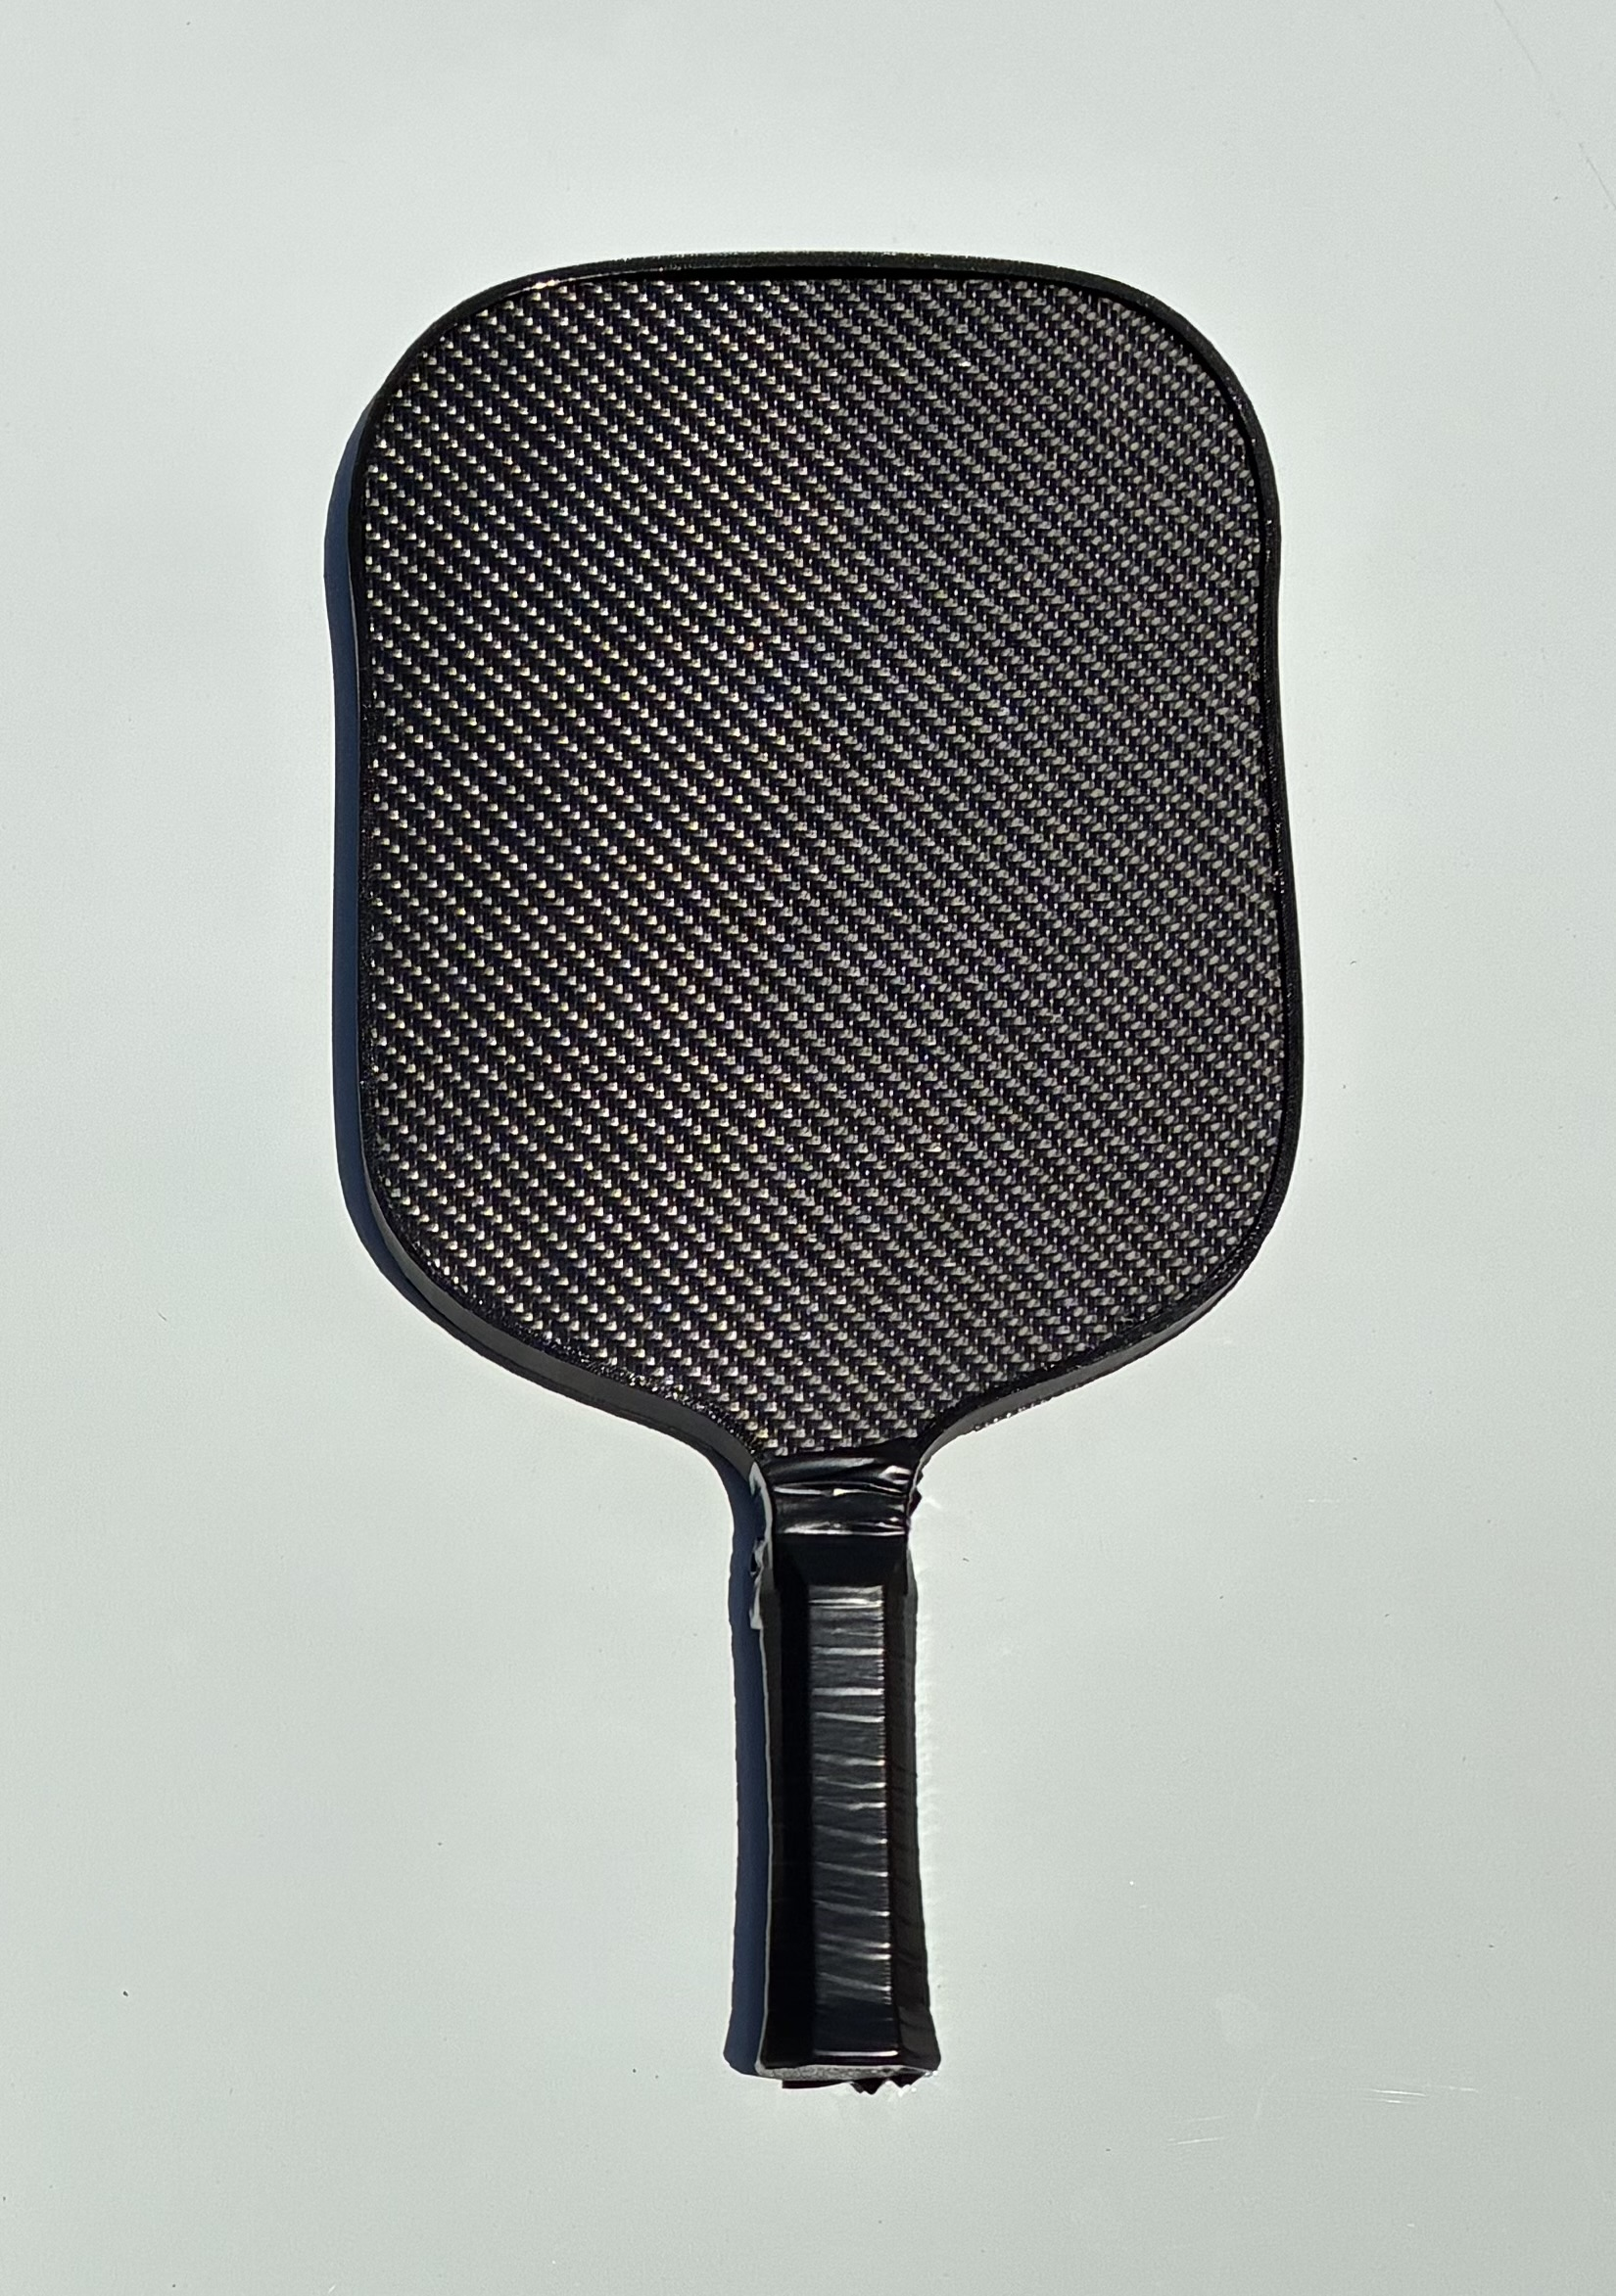
\includegraphics[
        width=3.72in,
        height=3.18in,
        keepaspectratio
    ]{full_assy}
};

\node[
    anchor=north,
    text=Muted,
    font=\sffamily\fontsize{6.9}{7.5}\selectfont
]
at ($(current page.north west)+(1.60in,-4.86in)$)
{Completed solo-built paddle assembly};

% ============================================================
% TOP CENTER — PROJECT OVERVIEW
% ============================================================

\fill[SoftGold,rounded corners=5pt]
    ($(current page.north west)+(2.95in,-1.62in)$)
    rectangle
    ($(current page.north west)+(5.53in,-4.86in)$);

\fill[PolyGold]
    ($(current page.north west)+(2.95in,-1.62in)$)
    rectangle
    ($(current page.north west)+(3.05in,-4.86in)$);

\node[
    anchor=north west,
    text=DeepGreen,
    font=\sffamily\bfseries\fontsize{8.0}{8.7}\selectfont
]
at ($(current page.north west)+(3.23in,-1.79in)$)
{PROJECT OVERVIEW};

\node[
    anchor=north west,
    align=left,
    text width=2.02in,
    text=Ink,
    font=\fontsize{7.05}{8.35}\selectfont
]
at ($(current page.north west)+(3.23in,-2.07in)$)
{
Independently designed and manufactured a lightweight prepreg
carbon-fiber pickleball paddle using a half-inch honeycomb
sandwich core, vacuum-bag consolidation, precision waterjet
trimming, and custom TPU and PLA components.

\vspace{5pt}

The project emphasized lightweight sandwich-composite design, repeatable manufacturing methods, dimensional accuracy, and the integration of custom 3D-printed TPU and PLA components into the final assembly.
};

\node[
    anchor=south west,
    align=left,
    text width=2.02in,
    text=PolyGold,
    font=\sffamily\bfseries\fontsize{6.65}{7.35}\selectfont
]
at ($(current page.north west)+(3.23in,-4.74in)$)
{
SOLE DESIGNER\\[2pt]
COMPOSITE FABRICATOR\\[2pt]
MANUFACTURING ENGINEER
};

% ============================================================
% TOP RIGHT — LAMINATE GRAPHIC
% ============================================================

\node[
    anchor=north west,
    inner sep=2.5pt,
    draw=DeepGreen,
    line width=0.65pt,
    rounded corners=5pt
]
at ($(current page.north west)+(5.71in,-1.62in)$)
{
    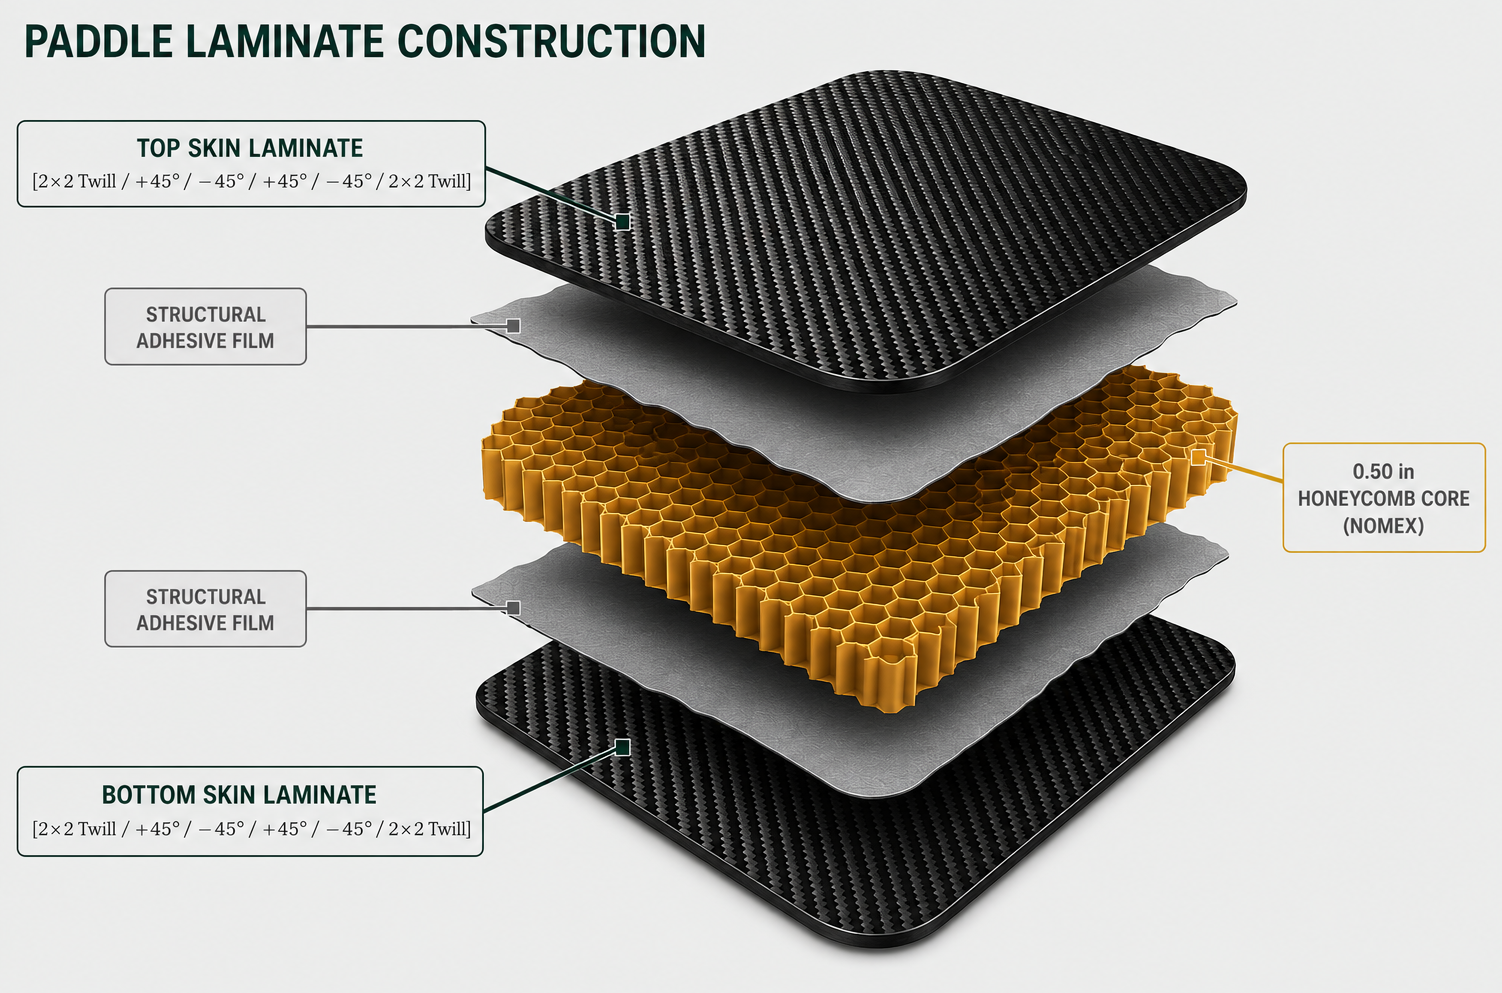
\includegraphics[
        width=4.80in,
        keepaspectratio
    ]{LAMINATE}
};

% ============================================================
% BOTTOM LEFT — SUPPORTING IMAGES
% ============================================================

\node[
    anchor=center,
    inner sep=3pt,
    draw=RuleGray,
    line width=0.55pt,
    rounded corners=4pt
]
at ($(current page.north west)+(1.12in,-5.98in)$)
{
    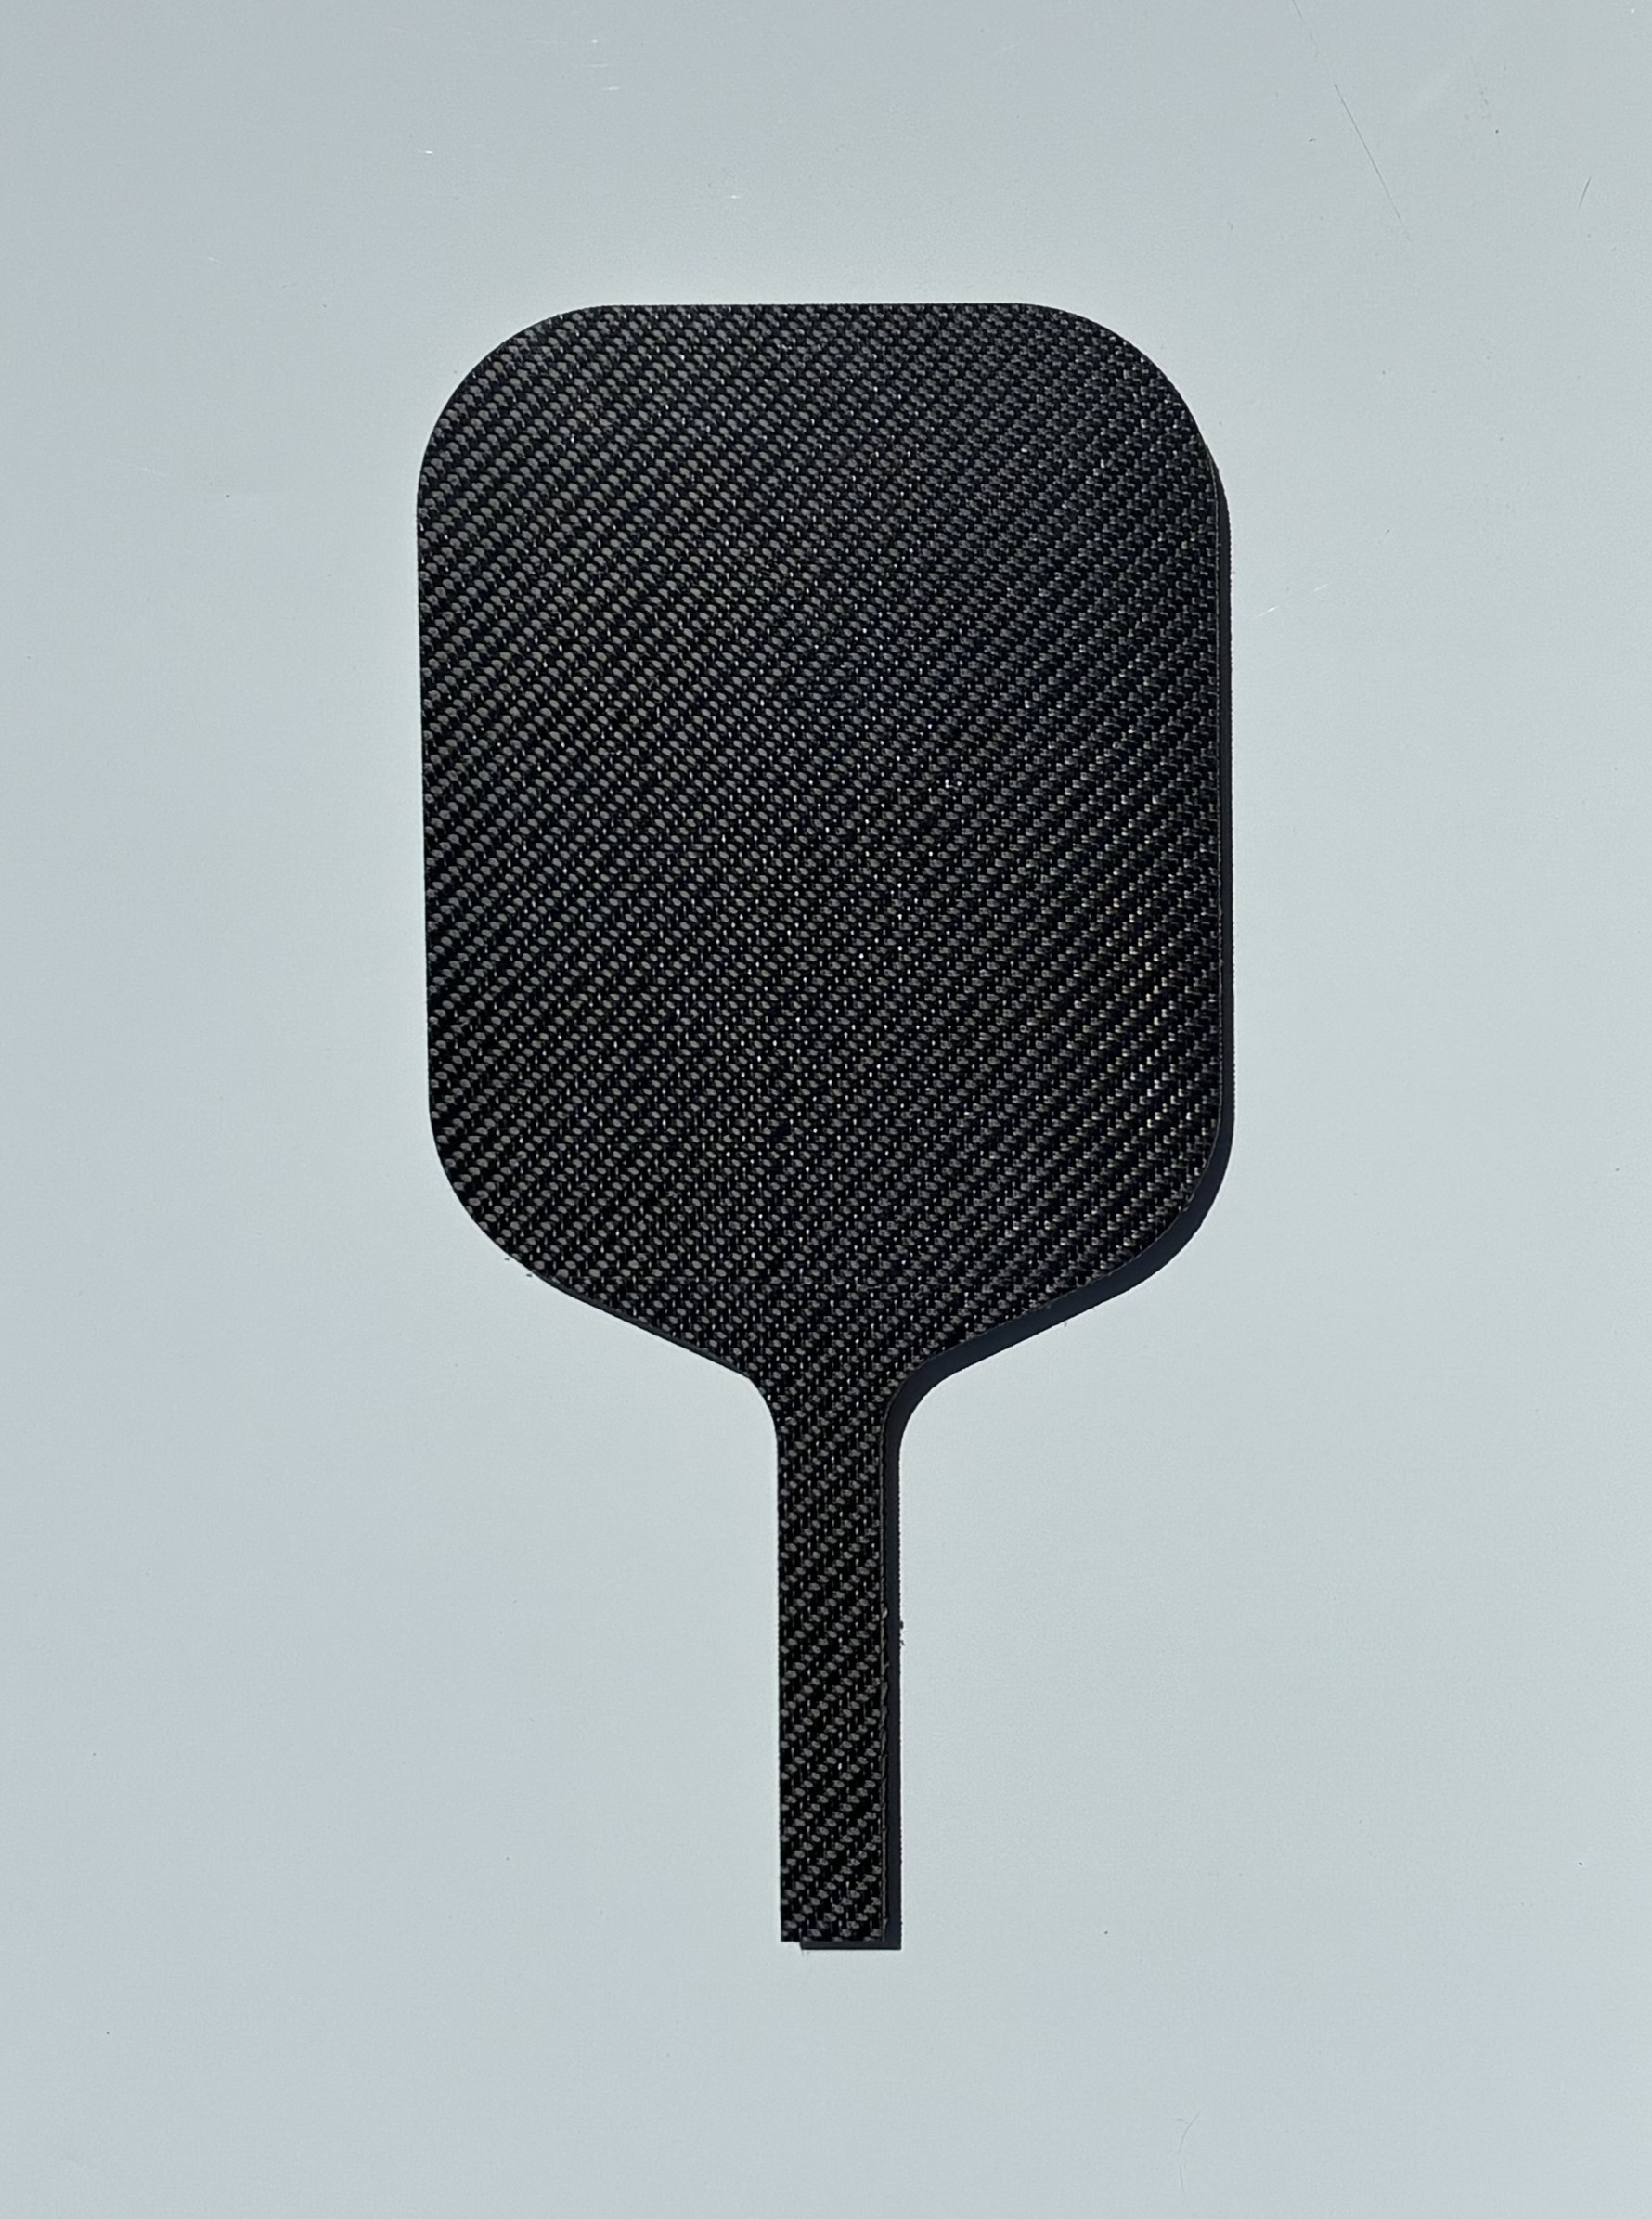
\includegraphics[
        width=1.30in,
        height=1.78in,
        keepaspectratio
    ]{front_view}
};

\node[
    anchor=center,
    inner sep=3pt,
    draw=RuleGray,
    line width=0.55pt,
    rounded corners=4pt
]
at ($(current page.north west)+(2.72in,-5.98in)$)
{
    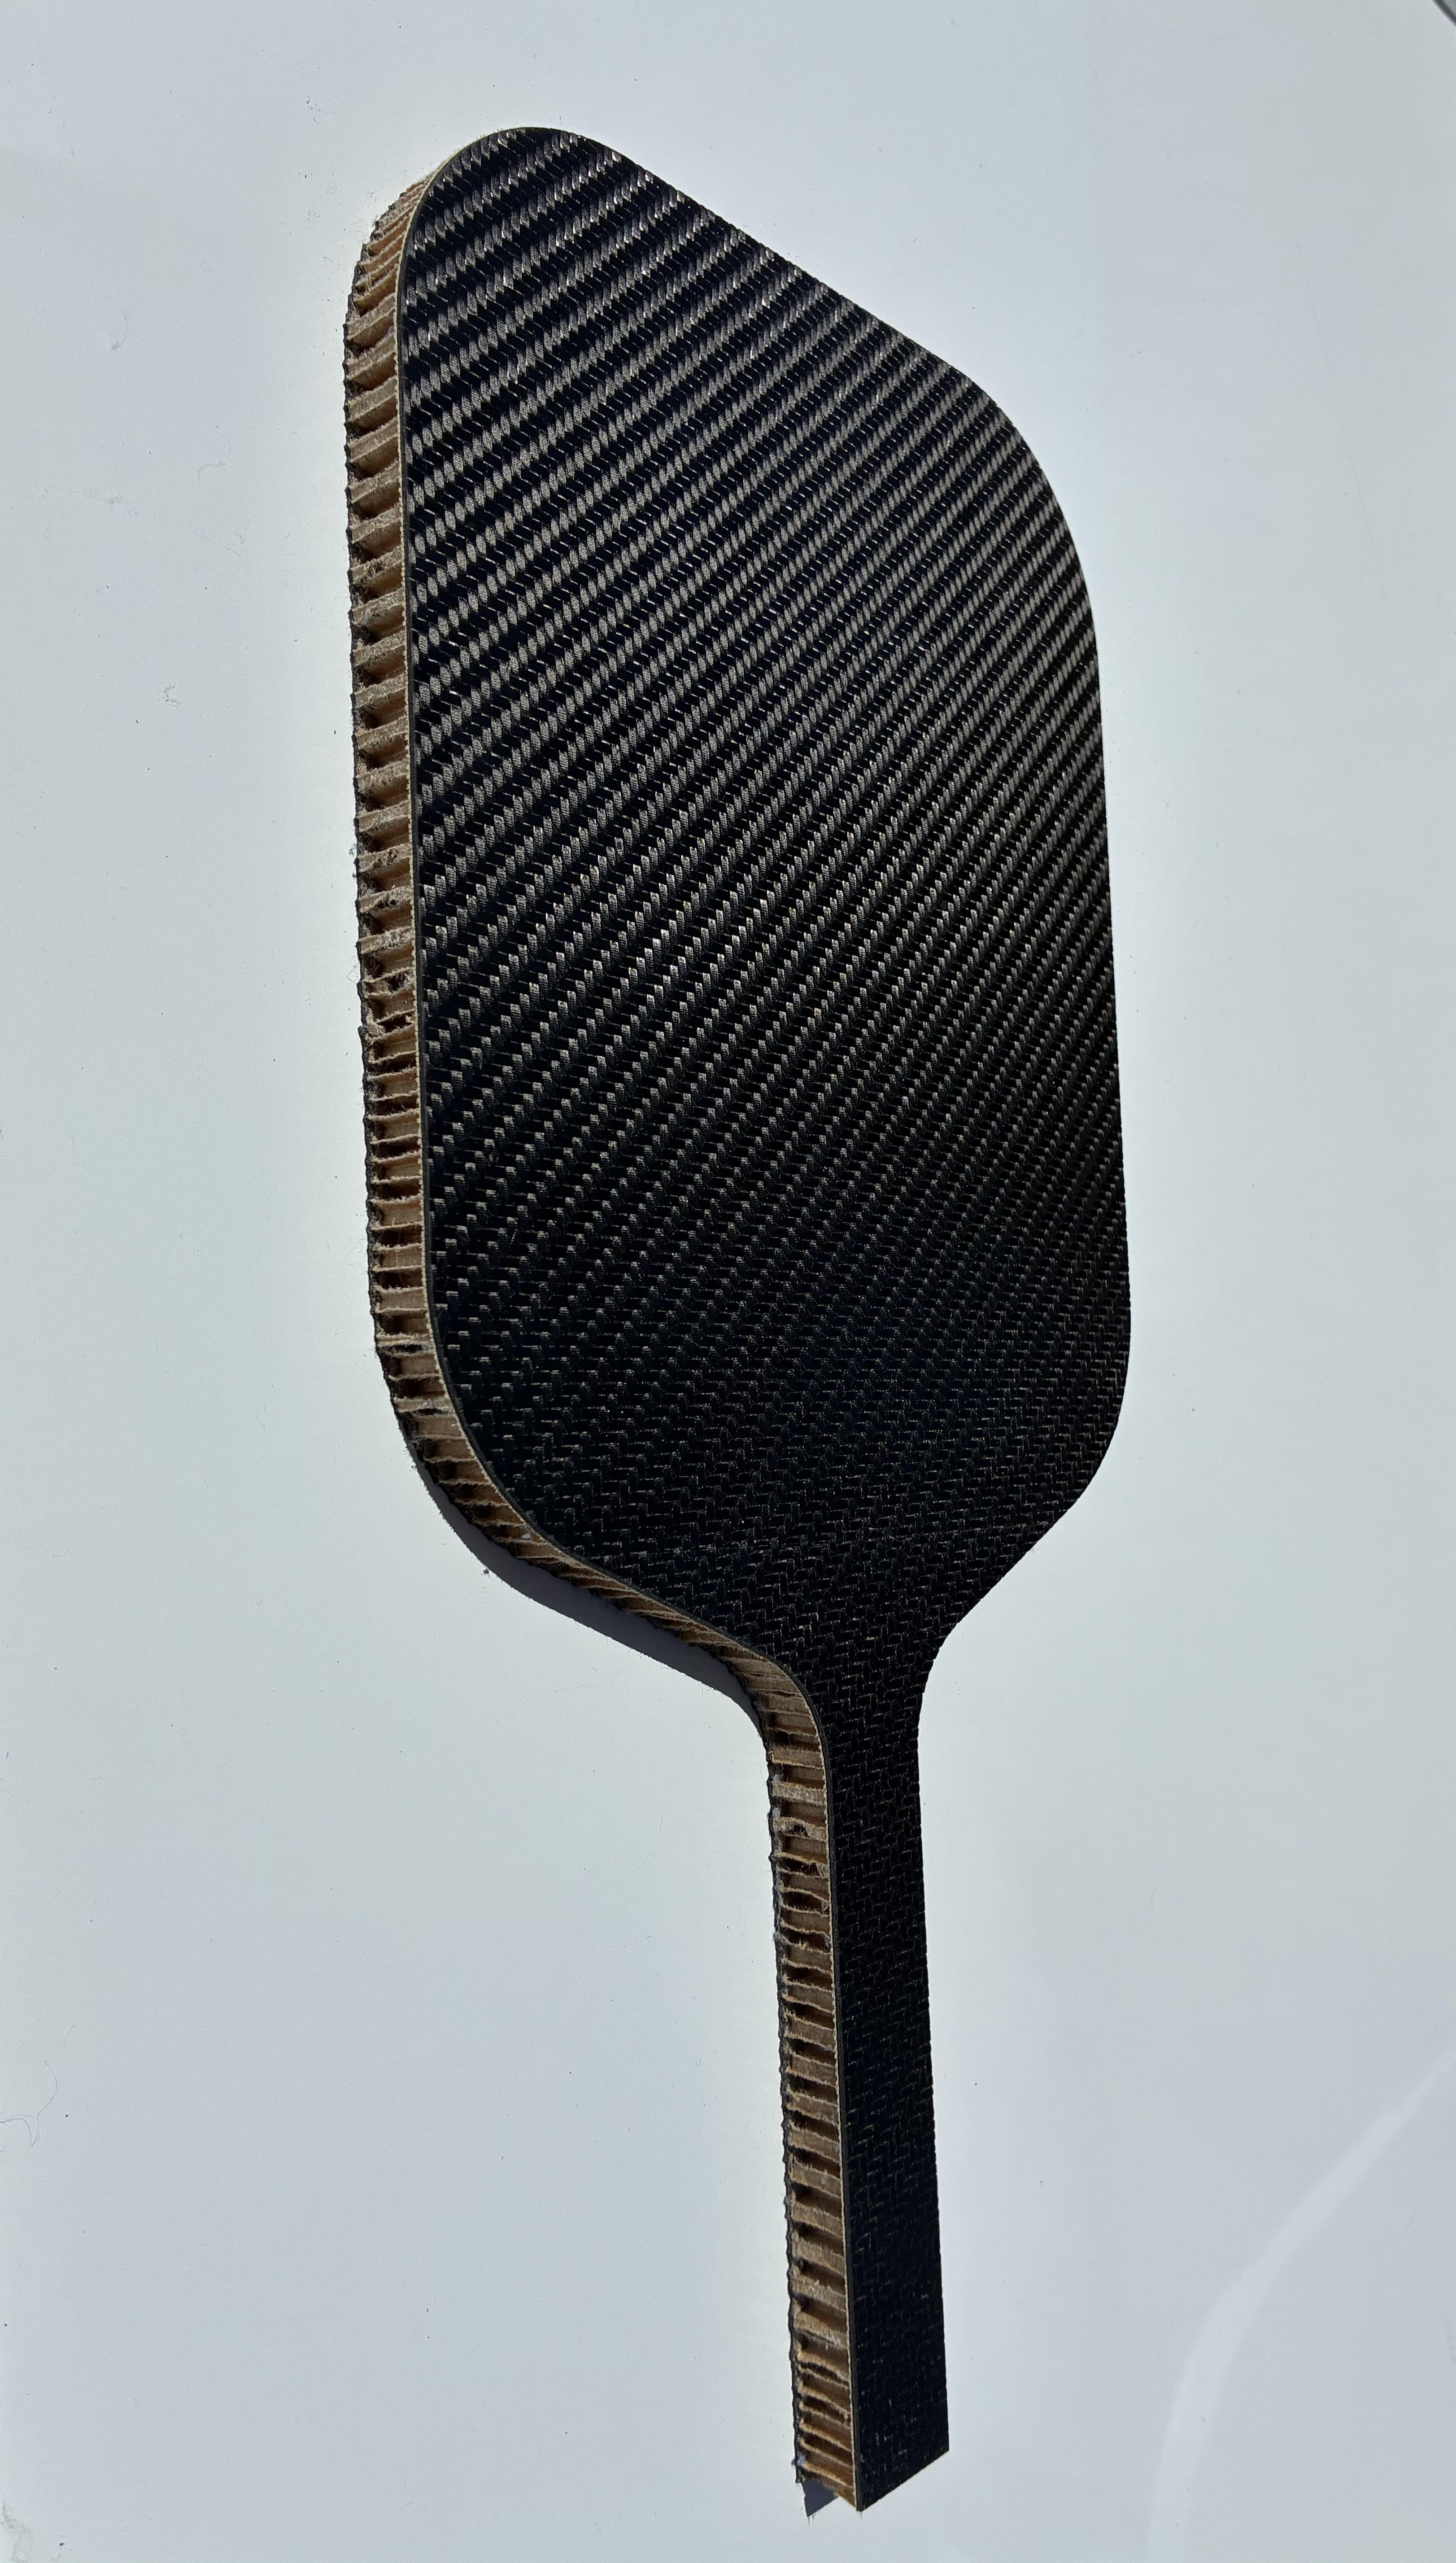
\includegraphics[
        width=1.30in,
        height=1.78in,
        keepaspectratio
    ]{side_core_view}
};

\node[
    anchor=center,
    inner sep=3pt,
    draw=RuleGray,
    line width=0.55pt,
    rounded corners=4pt
]
at ($(current page.north west)+(4.32in,-5.98in)$)
{
    \includegraphics[
        angle=-90,
        origin=c,
        width=1.30in,
        height=1.78in,
        keepaspectratio
    ]{waterjet}
};

\node[
    anchor=north,
    align=center,
    text width=1.38in,
    text=Muted,
    font=\sffamily\fontsize{6.5}{7.1}\selectfont
]
at ($(current page.north west)+(1.12in,-7.00in)$)
{Front view};

\node[
    anchor=north,
    align=center,
    text width=1.38in,
    text=Muted,
    font=\sffamily\fontsize{6.5}{7.1}\selectfont
]
at ($(current page.north west)+(2.72in,-7.00in)$)
{Core and edge profile};

\node[
    anchor=north,
    align=center,
    text width=1.38in,
    text=Muted,
    font=\sffamily\fontsize{6.5}{7.1}\selectfont
]
at ($(current page.north west)+(4.32in,-7.00in)$)
{Waterjet cutting setup};

% ============================================================
% BOTTOM RIGHT — MANUFACTURING HIGHLIGHTS
% ============================================================

\fill[SoftGreen,rounded corners=5pt]
    ($(current page.north west)+(5.18in,-5.05in)$)
    rectangle
    ($(current page.north east)+(-0.42in,-7.18in)$);

\draw[RuleGray,line width=0.55pt,rounded corners=5pt]
    ($(current page.north west)+(5.18in,-5.05in)$)
    rectangle
    ($(current page.north east)+(-0.42in,-7.18in)$);

\node[
    anchor=north west,
    text=DeepGreen,
    font=\sffamily\bfseries\fontsize{7.9}{8.6}\selectfont
]
at ($(current page.north west)+(5.44in,-5.20in)$)
{MANUFACTURING HIGHLIGHTS};

\node[
    anchor=north west,
    align=left,
    text width=5.05in,
    text=Ink,
    font=\fontsize{6.72}{7.82}\selectfont
]
at ($(current page.north west)+(5.44in,-5.49in)$)
{
\textbf{Consolidation.}
Vacuum bagging and distributed weight pressure maintained intimate contact
throughout the prepreg sandwich layup.\\[2.4pt]
\textbf{Surface quality.}
A scarce PTFE release film produced an unusually consistent matte finish
with a subtle sheen and minimal post-processing.\\[2.4pt]
\textbf{Waterjet stability.}
Perimeter weights restrained the cured stock against jet-induced lifting
and rotational moments during cutting.\\[2.4pt]
\textbf{Final assembly.}
A printed TPU edge band protected the carbon perimeter, while the PLA handle
used clearance cutouts to accommodate future stock-thickness and cutting variation.
};

% ============================================================
% RESOURCE LINK
% ============================================================

\node[
    anchor=north,
    align=center,
    text=DeepGreen,
    font=\sffamily\bfseries\fontsize{7.0}{7.6}\selectfont
]
at ($(current page.north)+(0,-7.42in)$)
{\href{\PaddleWaterjetVideo}
{\faPlayCircle\ WATERJET PICKLEBALL PADDLE DEMONSTRATION}};

% ============================================================
% FOOTER
% ============================================================

\node[
    anchor=south west,
    text=white,
    font=\sffamily\bfseries\fontsize{7.1}{7.7}\selectfont
]
at ($(current page.south west)+(0.42in,0.17in)$)
{\hyperlink{toro-results}{\faArrowLeft\ TORO COVER}};

\node[
    anchor=south,
    text=white,
    font=\sffamily\fontsize{7.0}{7.6}\selectfont
]
at ($(current page.south)+(0,0.17in)$)
{PICKLEBALL PADDLE \hspace{6pt} 1 / 1};

\node[
    anchor=south east,
    text=white,
    font=\sffamily\bfseries\fontsize{7.1}{7.7}\selectfont
]
at ($(current page.south east)+(-0.42in,0.17in)$)
{NEXT PROJECT \faArrowRight};

\end{tikzpicture}
%\input{Beam}
%\clearpage

\clearpage
.
% 2. In main.tex, place 
% ============================================================
% TORO COVER — THREE-PAGE PORTFOLIO CASE STUDY
% Pages 3–5 of the complete portfolio
%
% IMPORTANT:
% 1. This file must NOT contain \documentclass, \begin{document},
%    \end{document}, or 
% ============================================================
% TORO COVER — THREE-PAGE PORTFOLIO CASE STUDY
% Pages 3–5 of the complete portfolio
%
% IMPORTANT:
% 1. This file must NOT contain \documentclass, \begin{document},
%    \end{document}, or \input{toro}.
% 2. In main.tex, place \input{toro} before \end{document}.
% 3. Image references use the original Overleaf base filenames
%    without extensions.
% ============================================================



% ============================================================
% CLICKABLE PROJECT RESOURCES
% All links use the exact Google Drive resources supplied.
% ============================================================
\providecommand{\ToroDrawingLink}{https://drive.google.com/file/d/1A7-7wMnRNLuQDaTgxeuUCBsGNqyXzOGV/view?usp=sharing}
\providecommand{\ToroDimensionsLink}{https://drive.google.com/file/d/13sw3BNJvE8GdzlRffxoF2n5r9Gzxide7/view?usp=sharing}
\providecommand{\ToroProblemLink}{https://drive.google.com/file/d/1zHtl8zrb13F1yeN74ptawpfS5UM_xsuw/view?usp=drive_link}
\providecommand{\ToroReportLink}{https://drive.google.com/file/d/1ULZ-P46lFsC2x29ZfmRVIKgYnr9o8hMt/view?usp=drive_link}
\providecommand{\ToroPosterLink}{https://drive.google.com/file/d/1vKiKaJUcHQb_db-FkZnRF6EvtuM4hKyS/view?usp=drive_link}
\providecommand{\ToroDeploymentLink}{https://drive.google.com/file/d/1XJx34o80_mZPTl7xy93HtWAgtS3ThhvY/view?usp=drive_link}
\providecommand{\ToroRemovalLink}{https://drive.google.com/file/d/1O7xYeyB67NUwT-j1B1HeiCcHnZDYjk6_/view?usp=drive_link}

% ============================================================
% PAGE 1 — PROJECT OVERVIEW, OWNERSHIP, AND ARCHITECTURE
% ============================================================

\clearpage
\thispagestyle{empty}
\hypertarget{toro}{}
\null

\begin{tikzpicture}[remember picture,overlay]

% Background
\fill[white]
    (current page.south west)
    rectangle
    (current page.north east);

% Page bars
\fill[DeepGreen]
    (current page.north west)
    rectangle
    ($(current page.north east)+(0,-0.095in)$);

\fill[PolyGold]
    ($(current page.north west)+(0,-0.095in)$)
    rectangle
    ($(current page.north east)+(0,-0.14in)$);

\fill[DeepGreen]
    (current page.south west)
    rectangle
    ($(current page.south east)+(0,0.36in)$);

\fill[PolyGold]
    ($(current page.south west)+(0,0.36in)$)
    rectangle
    ($(current page.south east)+(0,0.405in)$);

% Header
\node[
    anchor=north west,
    text=PolyGold,
    font=\sffamily\bfseries\fontsize{8.1}{8.7}\selectfont
]
at ($(current page.north west)+(0.42in,-0.39in)$)
{01 COMPOSITES \hspace{5pt}/\hspace{5pt} PROJECT 01};

\node[
    anchor=north west,
    text=DeepGreen,
    font=\bfseries\fontsize{23.5}{24.5}\selectfont
]
at ($(current page.north west)+(0.40in,-0.67in)$)
{TORO CARBON FIBER SAFETY COVER};

\node[
    anchor=north west,
    text=Muted,
    font=\sffamily\fontsize{8.4}{9.2}\selectfont
]
at ($(current page.north west)+(0.42in,-1.12in)$)
{Cal Poly Composites Laboratory \hspace{7pt}\textbullet\hspace{7pt}
Team Project \hspace{7pt}\textbullet\hspace{7pt}
Fall--Spring 2026 \hspace{7pt}\textbullet\hspace{7pt}
San Luis Obispo, California};

\fill[PolyGold]
    ($(current page.north west)+(0.42in,-1.37in)$)
    rectangle
    ($(current page.north west)+(6.1in,-1.325in)$);

% Challenge text
\node[
    anchor=north west,
    text=DeepGreen,
    font=\sffamily\bfseries\fontsize{8.1}{8.8}\selectfont
]
at ($(current page.north west)+(0.43in,-1.61in)$)
{THE CHALLENGE};

\node[
    anchor=north west,
    align=left,
    text width=4.47in,
    text=Ink,
    font=\fontsize{8.05}{9.65}\selectfont
]
at ($(current page.north west)+(0.43in,-1.84in)$)
{
Develop a lightweight cover for a 6 ft by 6 ft in-ground spa
that could be deployed by one person, stored compactly,
provide insulation, resist a poolside environment, and maintain
a refined appearance. The sponsor supplied an ambitious but
intentionally broad project statement, requiring the team to
define the product architecture, priorities, manufacturing
strategy, and realistic path toward future commercialization.
};

% Role box
\fill[SoftGold,rounded corners=5pt]
    ($(current page.north west)+(0.42in,-2.88in)$)
    rectangle
    ($(current page.north west)+(4.98in,-4.58in)$);

\fill[PolyGold]
    ($(current page.north west)+(0.42in,-2.88in)$)
    rectangle
    ($(current page.north west)+(0.52in,-4.58in)$);

\node[
    anchor=north west,
    text=DeepGreen,
    font=\sffamily\bfseries\fontsize{8.1}{8.8}\selectfont
]
at ($(current page.north west)+(0.66in,-3.02in)$)
{MY ROLE — DESIGN \& MANUFACTURING LEAD};

\node[
    anchor=north west,
    align=left,
    text width=4.02in,
    text=Ink,
    font=\fontsize{7.05}{8.15}\selectfont
]
at ($(current page.north west)+(0.66in,-3.27in)$)
{
\textbullet\ Modeled every custom part and the complete assembly\\[1.5pt]
\textbullet\ Produced the engineering drawing package independently\\[1.5pt]
\textbullet\ Developed the composite-panel manufacturing process\\[1.5pt]
\textbullet\ Created all waterjet DXFs and manufacturing geometry\\[1.5pt]
\textbullet\ Trained teammates in wet layup and vacuum bagging\\[1.5pt]
\textbullet\ Presented feasibility, scope, and tradeoffs to the sponsor
};

% Large deployed foam-model image
\node[anchor=center,inner sep=0pt]
at ($(current page.north west)+(8.00in,-3.04in)$)
{
    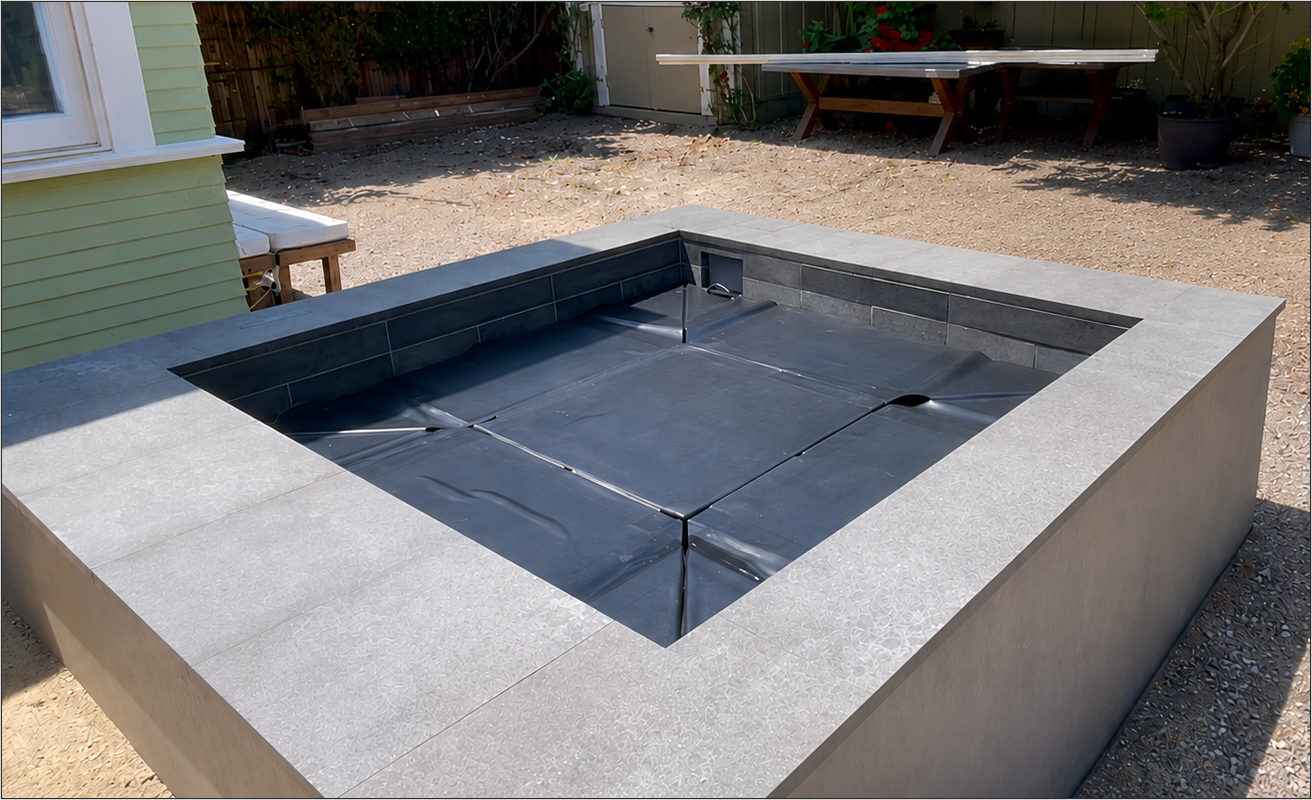
\includegraphics[
        width=5.55in,
        height=2.78in,
        keepaspectratio
    ]{deployed_functional_prototype}
};

\draw[DeepGreen,line width=0.8pt,rounded corners=7pt]
    ($(current page.north west)+(5.16in,-1.61in)$)
    rectangle
    ($(current page.north east)+(-0.42in,-4.47in)$);

\node[
    anchor=north west,
    text=Muted,
    font=\sffamily\fontsize{6.2}{6.9}\selectfont
]
at ($(current page.north west)+(5.18in,-4.54in)$)
{Functional foam model deployed over the sponsor's in-ground spa.};

% Image-strip title
\node[
    anchor=north west,
    text=DeepGreen,
    font=\sffamily\bfseries\fontsize{8.1}{8.8}\selectfont
]
at ($(current page.north west)+(0.43in,-4.78in)$)
{PRODUCT DEVELOPMENT AND FINAL ARCHITECTURE};

% Five-image development strip — CAD-first sequence
% Image 1: topside CAD
\node[anchor=center,inner sep=0pt]
at ($(current page.north west)+(1.47in,-5.73in)$)
{
    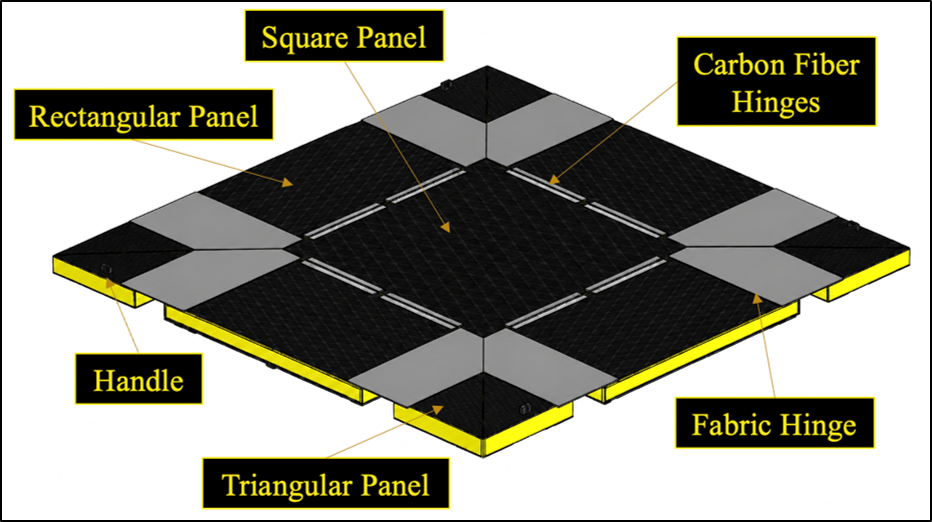
\includegraphics[
        width=1.92in,
        height=1.30in,
        keepaspectratio
    ]{Toro_Cover_topside_Cad}
};
\draw[RuleGray,line width=0.55pt,rounded corners=4pt]
    ($(current page.north west)+(0.43in,-5.04in)$)
    rectangle
    ($(current page.north west)+(2.51in,-6.43in)$);

% Image 2: underside CAD
\node[anchor=center,inner sep=0pt]
at ($(current page.north west)+(3.66in,-5.73in)$)
{
    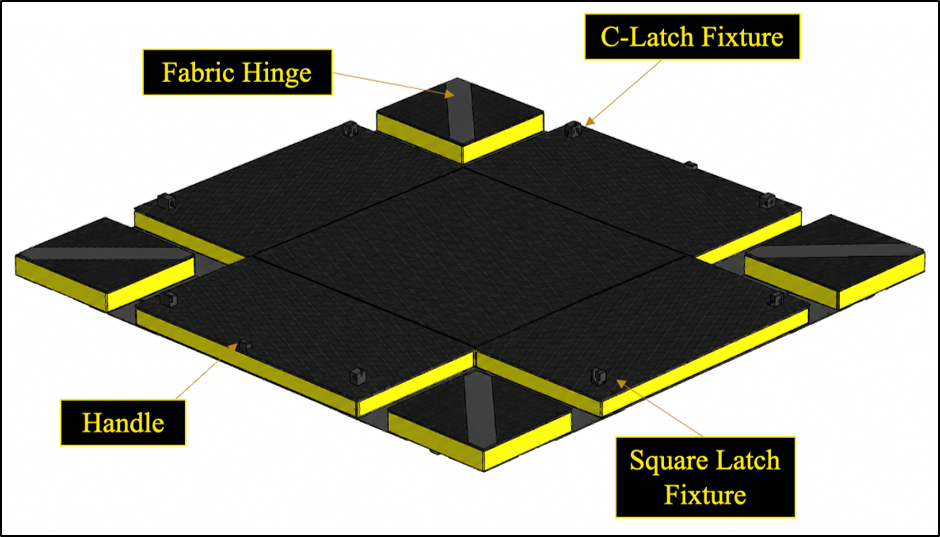
\includegraphics[
        width=1.92in,
        height=1.30in,
        keepaspectratio
    ]{toro_cover_underside_cad}
};
\draw[RuleGray,line width=0.55pt,rounded corners=4pt]
    ($(current page.north west)+(2.62in,-5.04in)$)
    rectangle
    ($(current page.north west)+(4.70in,-6.43in)$);

% Image 3: folded CAD
\node[anchor=center,inner sep=0pt]
at ($(current page.north west)+(5.85in,-5.73in)$)
{
    \includegraphics[
        width=1.92in,
        height=1.30in,
        keepaspectratio
    ]{\detokenize{Toro_Cover_folded Configuration}}
};
\draw[RuleGray,line width=0.55pt,rounded corners=4pt]
    ($(current page.north west)+(4.81in,-5.04in)$)
    rectangle
    ($(current page.north west)+(6.89in,-6.43in)$);

% Image 4: dual-use product concept
\node[anchor=center,inner sep=0pt]
at ($(current page.north west)+(8.04in,-5.73in)$)
{
    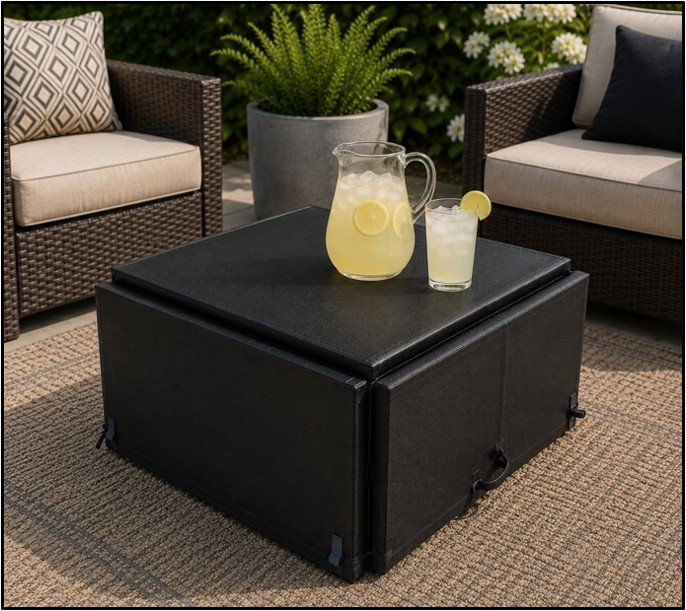
\includegraphics[
        width=1.92in,
        height=1.30in,
        keepaspectratio
    ]{generative_AI_concept_toro_cover_art}
};
\draw[RuleGray,line width=0.55pt,rounded corners=4pt]
    ($(current page.north west)+(7.00in,-5.04in)$)
    rectangle
    ($(current page.north west)+(9.08in,-6.43in)$);

% Image 5: folded foam functional prototype
% The portrait photograph is deliberately clipped to the landscape frame
% so the ottoman fills the card without extending beyond its border.
\begin{scope}
\clip[rounded corners=4pt]
    ($(current page.north west)+(9.19in,-5.04in)$)
    rectangle
    ($(current page.north east)+(-0.43in,-6.43in)$);

% Keep the original image proportions and center it within the existing card.
\node[anchor=center,inner sep=0pt]
at ($(current page.north west)+(9.88in,-5.735in)$)
{
    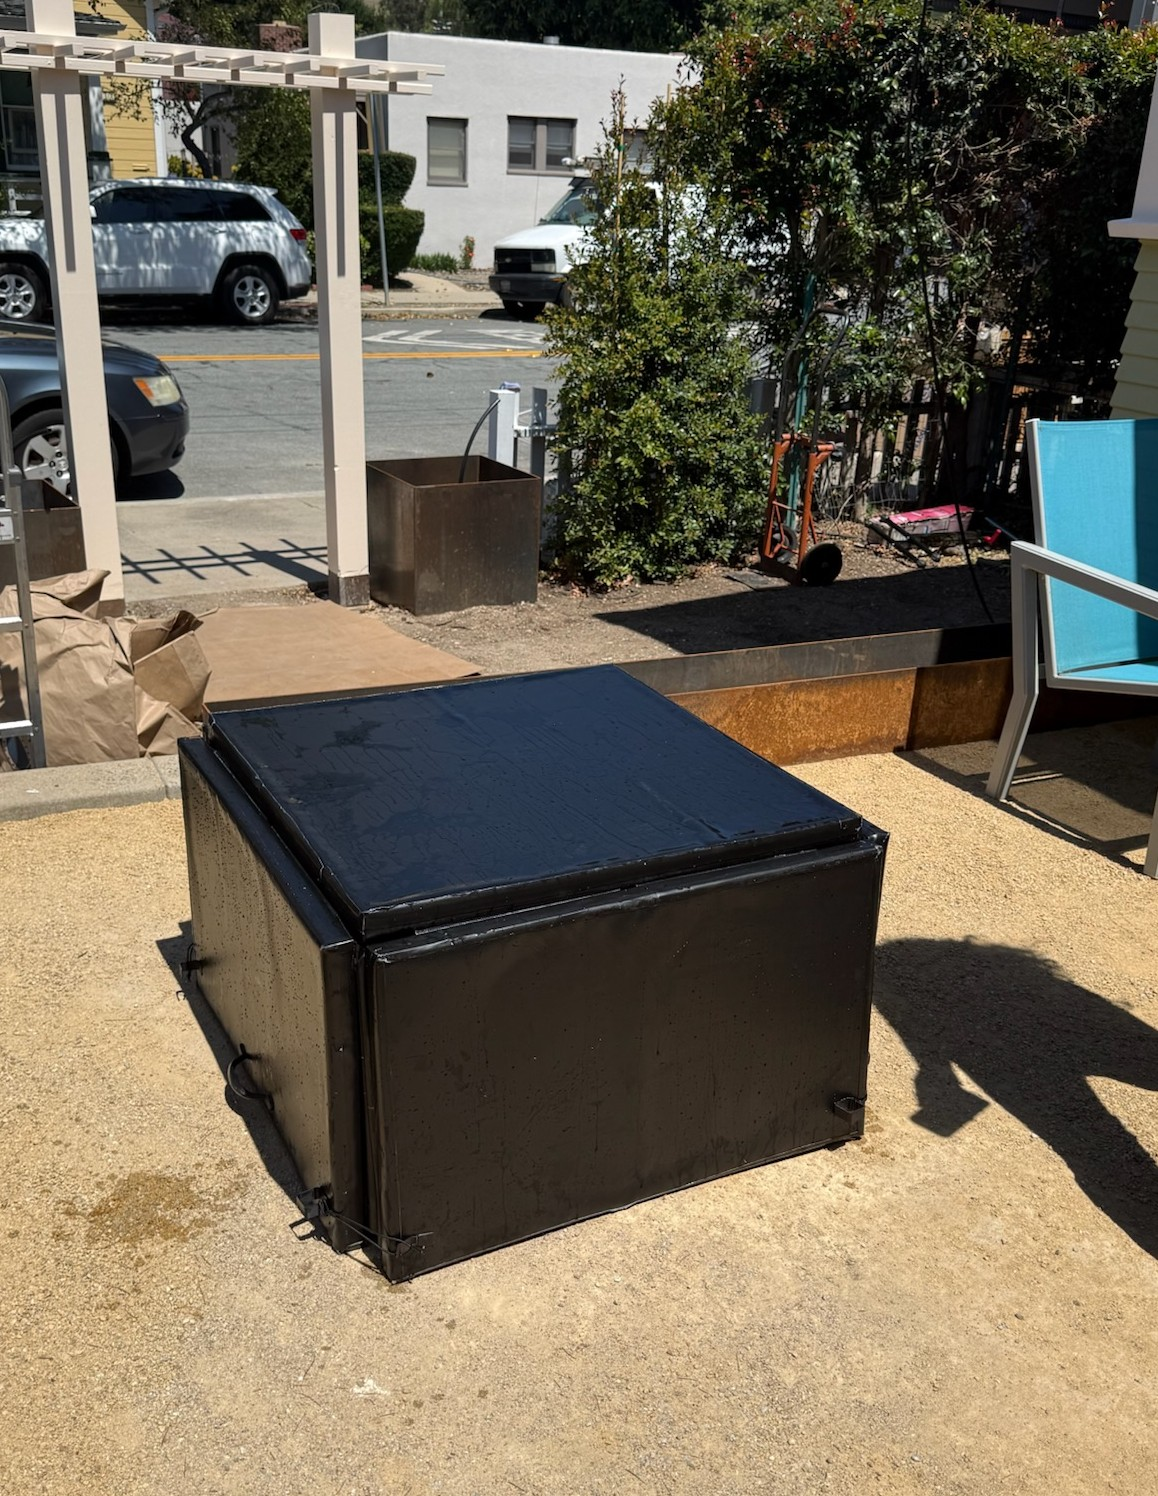
\includegraphics[
        width=1.58in,
        height=1.28in,
        keepaspectratio
    ]{foam_model_folded_backyard_image}
};
\end{scope}

\draw[RuleGray,line width=0.55pt,rounded corners=4pt]
    ($(current page.north west)+(9.19in,-5.04in)$)
    rectangle
    ($(current page.north east)+(-0.43in,-6.43in)$);

% Larger captions
\node[anchor=north,align=center,text width=1.95in,text=Muted,
      font=\sffamily\fontsize{6.8}{7.4}\selectfont]
at ($(current page.north west)+(1.47in,-6.49in)$)
{Topside panel architecture};

\node[anchor=north,align=center,text width=1.95in,text=Muted,
      font=\sffamily\fontsize{6.8}{7.4}\selectfont]
at ($(current page.north west)+(3.66in,-6.49in)$)
{Underside hinge architecture};

\node[anchor=north,align=center,text width=1.95in,text=Muted,
      font=\sffamily\fontsize{6.8}{7.4}\selectfont]
at ($(current page.north west)+(5.85in,-6.49in)$)
{Folded CAD configuration};

\node[anchor=north,align=center,text width=1.95in,text=Muted,
      font=\sffamily\fontsize{6.8}{7.4}\selectfont]
at ($(current page.north west)+(8.04in,-6.49in)$)
{Dual-use product vision};

\node[anchor=north,align=center,text width=1.95in,text=Muted,
      font=\sffamily\fontsize{6.8}{7.4}\selectfont]
at ($(current page.north west)+(9.88in,-6.49in)$)
{Folded foam prototype};

% Page 1 resource bar — centered and non-repeated resources
\fill[Panel,rounded corners=4pt]
    ($(current page.north west)+(0.43in,-7.05in)$)
    rectangle
    ($(current page.north east)+(-0.43in,-7.64in)$);
\draw[RuleGray,line width=0.5pt,rounded corners=4pt]
    ($(current page.north west)+(0.43in,-7.05in)$)
    rectangle
    ($(current page.north east)+(-0.43in,-7.64in)$);

\node[
    anchor=center,
    align=center,
    text=DeepGreen,
    font=\sffamily\bfseries\fontsize{6.9}{7.5}\selectfont
]
at ($(current page.north)+(0,-7.345in)$)
{\href{\ToroDrawingLink}{\faDraftingCompass\ DRAWING PACKAGE}
\hspace{24pt}
\href{\ToroDimensionsLink}{\faImage\ DIMENSION STUDY}
\hspace{24pt}
\href{\ToroProblemLink}{\faFileImage\ PROBLEM STATEMENT}};

% Footer
\node[
    anchor=south west,
    text=white,
    font=\sffamily\bfseries\fontsize{7.1}{7.7}\selectfont
]
at ($(current page.south west)+(0.42in,0.17in)$)
{\hyperlink{composites}{\faArrowLeft\ COMPOSITES}};

\node[
    anchor=south,
    text=white,
    font=\sffamily\fontsize{7.0}{7.6}\selectfont
]
at ($(current page.south)+(0,0.17in)$)
{TORO COVER \hspace{6pt} 1 / 3};

\node[
    anchor=south east,
    text=white,
    font=\sffamily\bfseries\fontsize{7.1}{7.7}\selectfont
]
at ($(current page.south east)+(-0.42in,0.17in)$)
{MANUFACTURING-DRIVEN DESIGN \faArrowRight};

\end{tikzpicture}


% ============================================================
% PAGE 2 — MANUFACTURING-DRIVEN DESIGN
% ============================================================

\clearpage
\thispagestyle{empty}
\hypertarget{toro-manufacturing}{}
\null

\begin{tikzpicture}[remember picture,overlay]

% Background and bars
\fill[white]
    (current page.south west)
    rectangle
    (current page.north east);

\fill[DeepGreen]
    (current page.north west)
    rectangle
    ($(current page.north east)+(0,-0.095in)$);

\fill[PolyGold]
    ($(current page.north west)+(0,-0.095in)$)
    rectangle
    ($(current page.north east)+(0,-0.14in)$);

\fill[DeepGreen]
    (current page.south west)
    rectangle
    ($(current page.south east)+(0,0.36in)$);

\fill[PolyGold]
    ($(current page.south west)+(0,0.36in)$)
    rectangle
    ($(current page.south east)+(0,0.405in)$);

% Header
\node[
    anchor=north west,
    text=PolyGold,
    font=\sffamily\bfseries\fontsize{8.1}{8.7}\selectfont
]
at ($(current page.north west)+(0.42in,-0.39in)$)
{TORO COVER \hspace{5pt}/\hspace{5pt} DESIGN FOR MANUFACTURABILITY};

\node[
    anchor=north west,
    text=DeepGreen,
    font=\bfseries\fontsize{23}{24}\selectfont
]
at ($(current page.north west)+(0.40in,-0.67in)$)
{THE ENVELOPE METHOD};

\node[
    anchor=north west,
    text=Muted,
    font=\sffamily\fontsize{8.7}{9.6}\selectfont
]
at ($(current page.north west)+(0.42in,-1.12in)$)
{A one-layup process developed for unusually thick insulated composite sandwich panels};

\fill[PolyGold]
    ($(current page.north west)+(0.42in,-1.36in)$)
    rectangle
    ($(current page.north west)+(5.30in,-1.315in)$);

% Process explanation
\fill[SoftGold,rounded corners=5pt]
    ($(current page.north west)+(0.42in,-1.61in)$)
    rectangle
    ($(current page.north east)+(-0.42in,-2.90in)$);

\fill[PolyGold]
    ($(current page.north west)+(0.42in,-1.61in)$)
    rectangle
    ($(current page.north west)+(0.52in,-2.90in)$);

\node[
    anchor=north west,
    text=DeepGreen,
    font=\sffamily\bfseries\fontsize{7.9}{8.6}\selectfont
]
at ($(current page.north west)+(0.67in,-1.76in)$)
{PROCESS INNOVATION};

\node[
    anchor=north west,
    align=left,
    text width=9.55in,
    text=Ink,
    font=\fontsize{7.35}{8.75}\selectfont
]
at ($(current page.north west)+(0.67in,-2.02in)$)
{
Weight reduction and insulation were both essential, leading to the selection of an
XPS foam core. Because XPS could not tolerate composite heat-cure temperatures, prepreg
processing was not practical and the panels had to be manufactured by wet layup with a
room-temperature cure. To simplify this process, I waterjet-cut XPS perimeter strips from
excess foam and placed them around each core inside the vacuum enclosure. Under vacuum,
the top and bottom carbon skins met along the panel sides and compressed against this
border, eliminating a separate edge-banding layup and reducing corner pleating.
};

% Workflow title
\node[
    anchor=north west,
    text=DeepGreen,
    font=\sffamily\bfseries\fontsize{8.0}{8.7}\selectfont
]
at ($(current page.north west)+(0.43in,-3.06in)$)
{MANUFACTURING WORKFLOW};

% Row 1 image 1
\node[anchor=center,inner sep=0pt]
at ($(current page.north west)+(2.07in,-4.105in)$)
{
    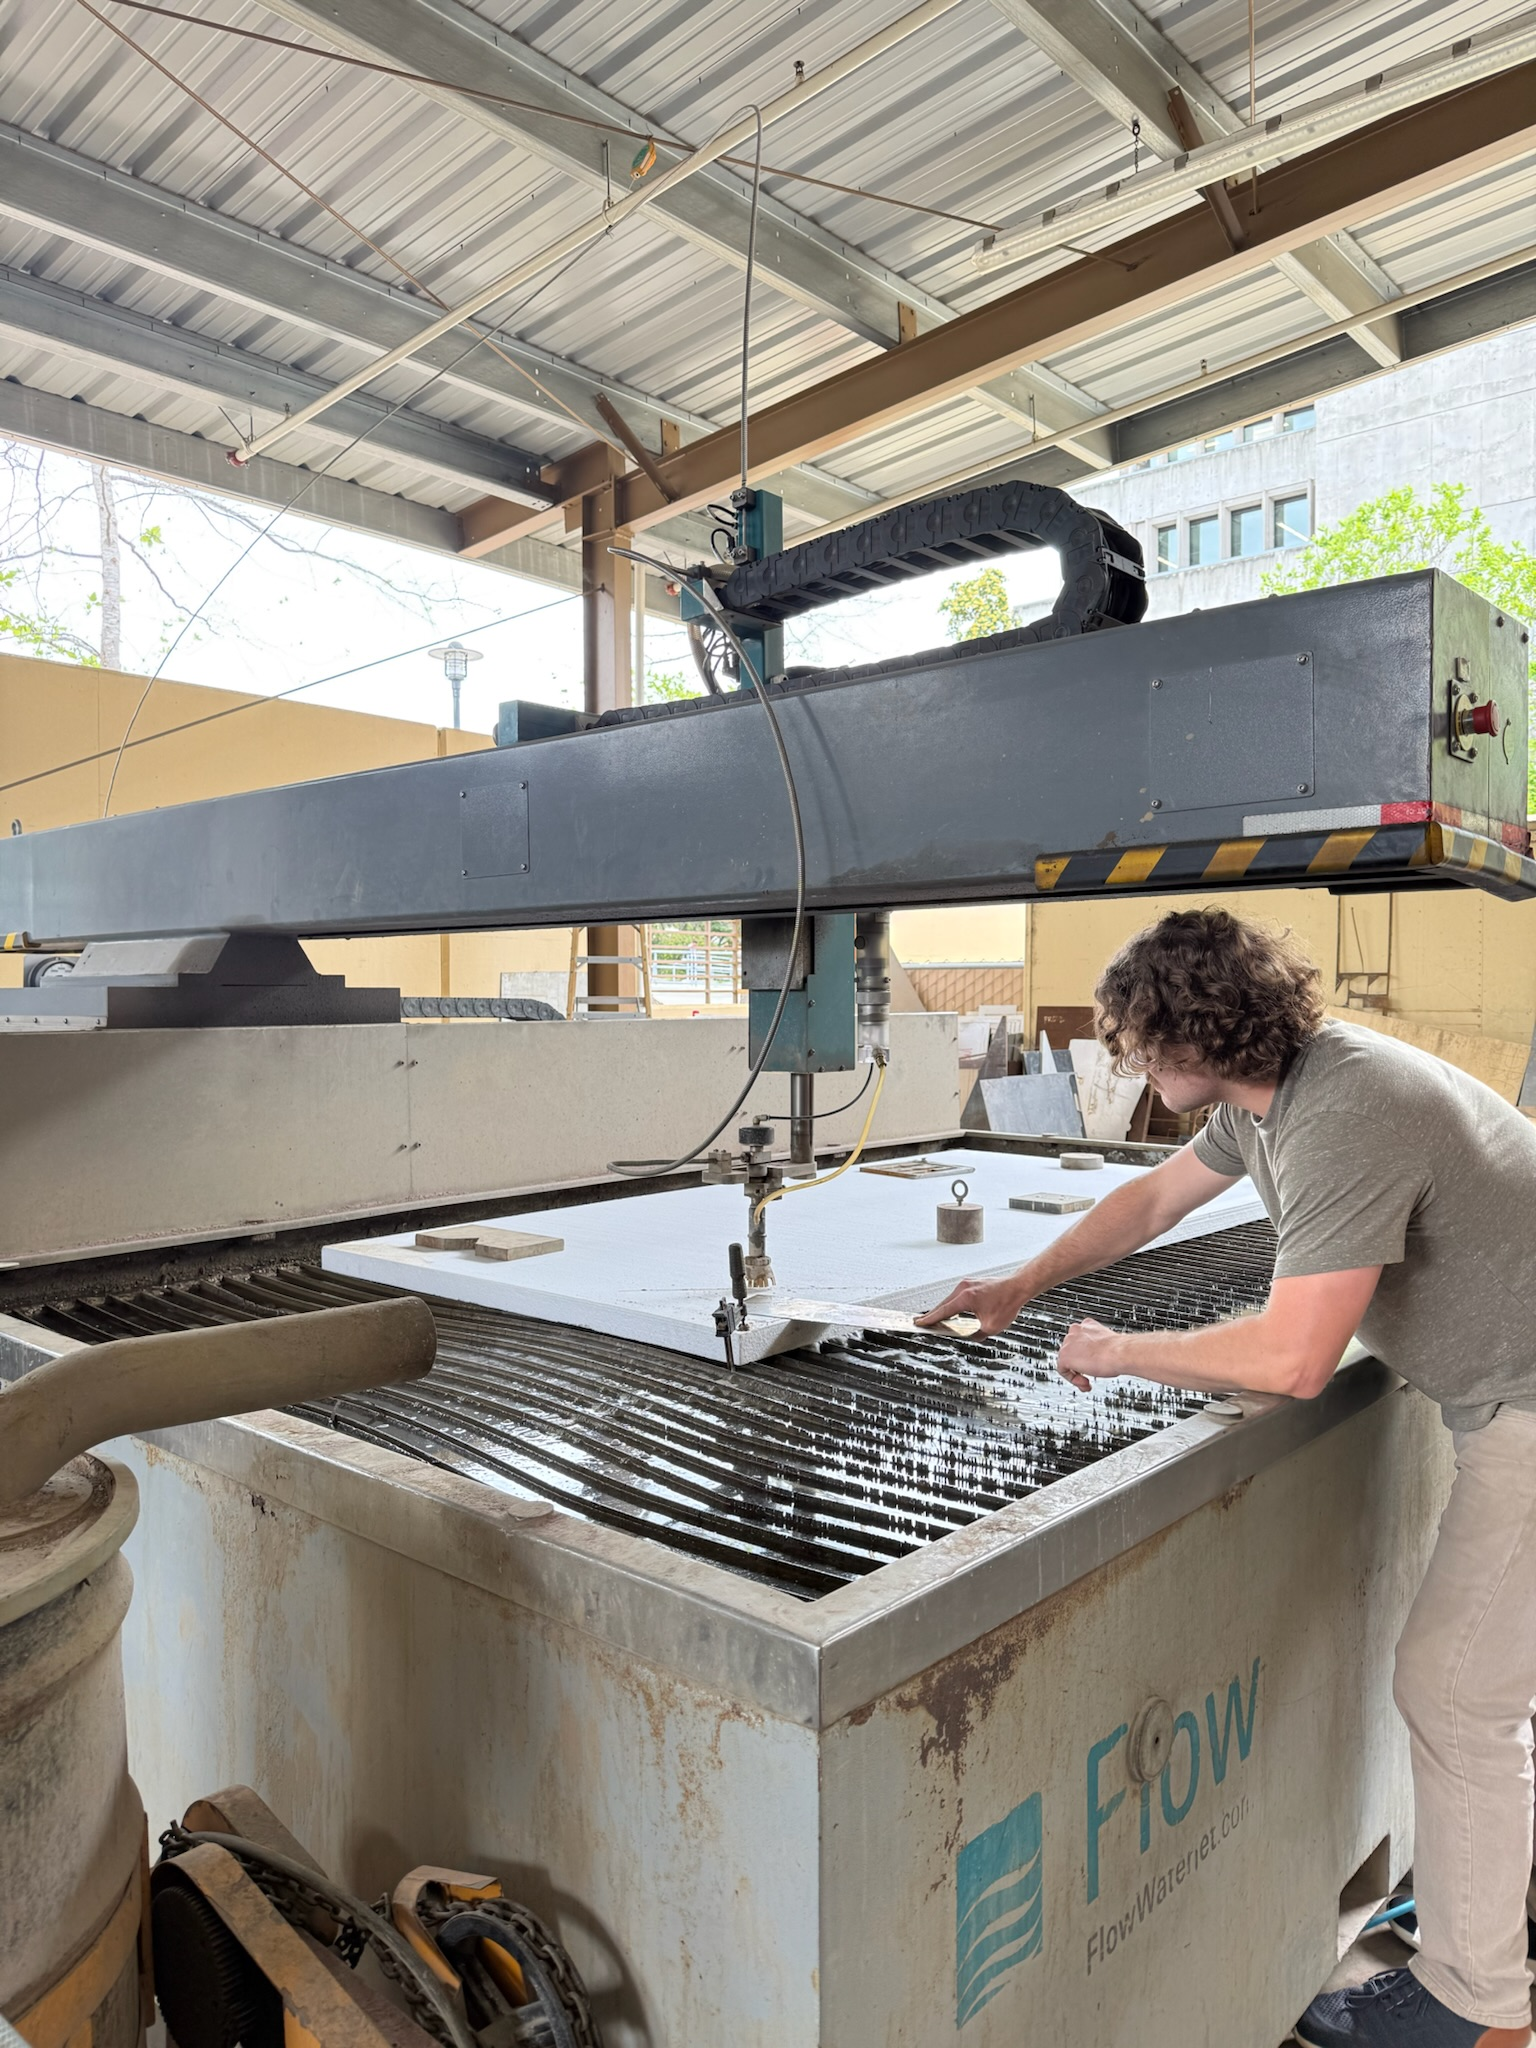
\includegraphics[
        width=3.10in,
        height=1.40in,
        keepaspectratio
    ]{waterjet_foam}
};
\draw[RuleGray,line width=0.55pt,rounded corners=4pt]
    ($(current page.north west)+(0.43in,-3.36in)$)
    rectangle
    ($(current page.north west)+(3.71in,-4.85in)$);

% Row 1 image 2
\node[anchor=center,inner sep=0pt]
at ($(current page.north west)+(5.50in,-4.105in)$)
{
    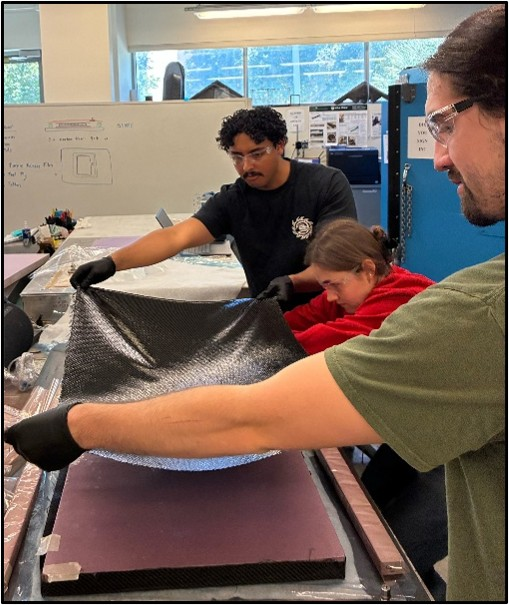
\includegraphics[
        width=3.10in,
        height=1.40in,
        keepaspectratio
    ]{group_layup}
};
\draw[RuleGray,line width=0.55pt,rounded corners=4pt]
    ($(current page.north west)+(3.86in,-3.36in)$)
    rectangle
    ($(current page.north west)+(7.14in,-4.85in)$);

% Row 1 image 3
\node[anchor=center,inner sep=0pt]
at ($(current page.north west)+(8.935in,-4.105in)$)
{
    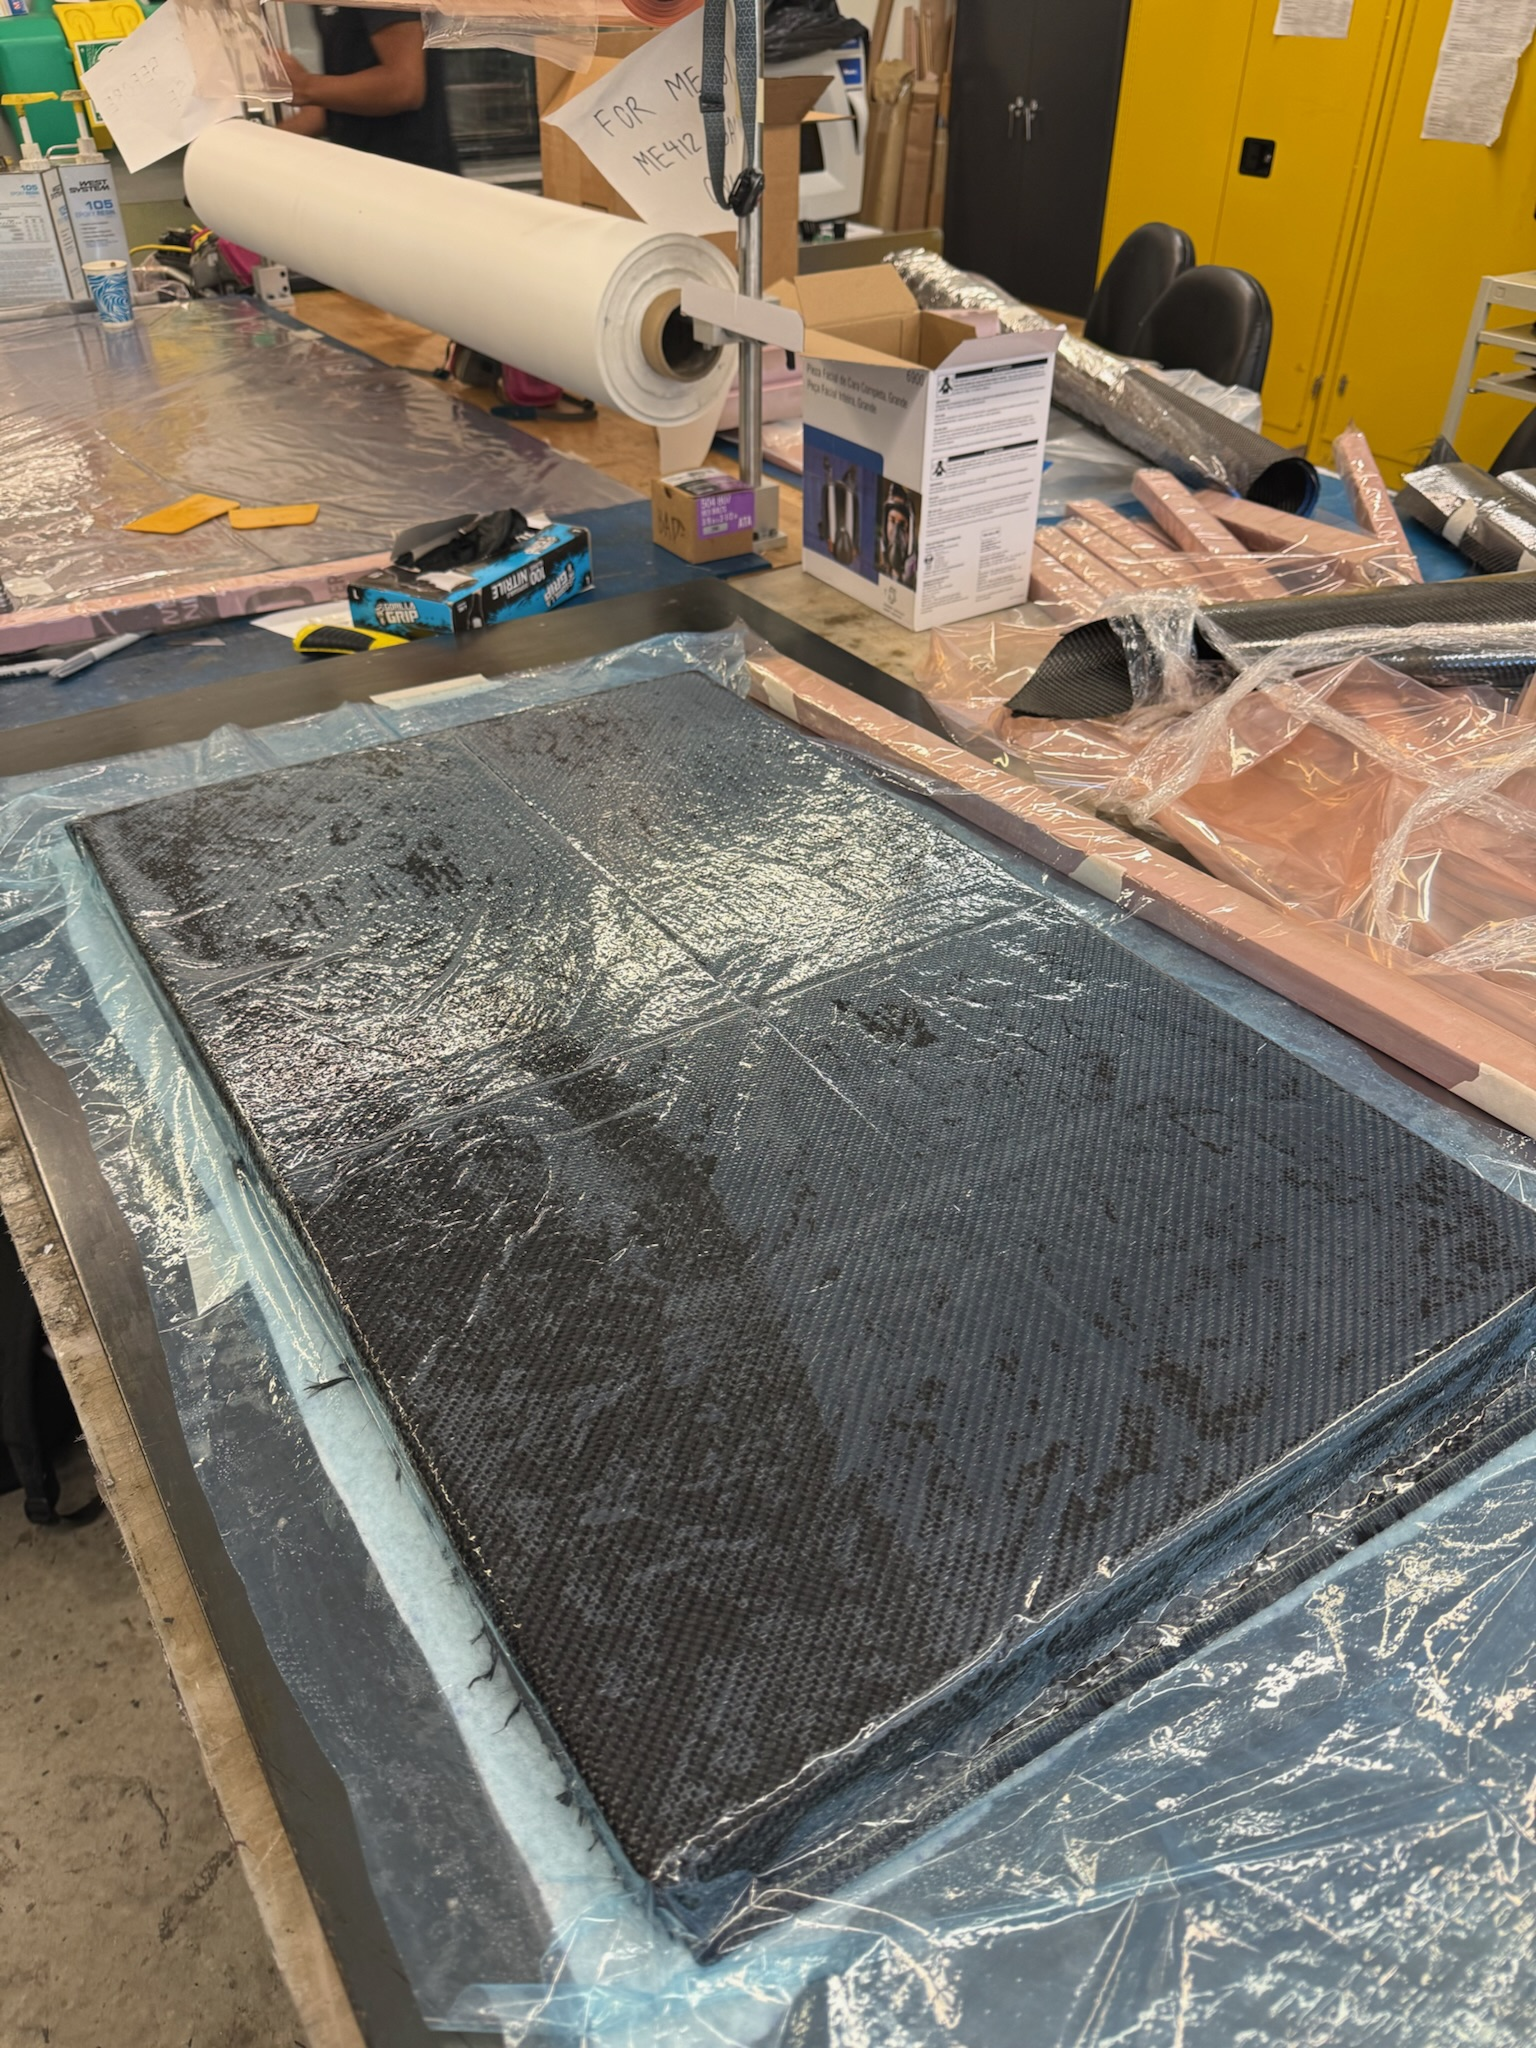
\includegraphics[
        width=3.10in,
        height=1.40in,
        keepaspectratio
    ]{blue_perforrated_film_layup}
};
\draw[RuleGray,line width=0.55pt,rounded corners=4pt]
    ($(current page.north west)+(7.29in,-3.36in)$)
    rectangle
    ($(current page.north east)+(-0.42in,-4.85in)$);

% Row 1 captions
\node[anchor=north,text=Muted,font=\sffamily\fontsize{6.7}{7.3}\selectfont]
at ($(current page.north west)+(2.07in,-4.90in)$)
{1. Waterjet-cut core and perimeter geometry};

\node[anchor=north,text=Muted,font=\sffamily\fontsize{6.7}{7.3}\selectfont]
at ($(current page.north west)+(5.50in,-4.90in)$)
{2. Team wet layup under my process guidance};

\node[anchor=north,text=Muted,font=\sffamily\fontsize{6.7}{7.3}\selectfont]
at ($(current page.north west)+(8.935in,-4.90in)$)
{3. Perforated film, breather, and vacuum enclosure};

% Row 2 image 1
\node[anchor=center,inner sep=0pt]
at ($(current page.north west)+(2.07in,-5.875in)$)
{
    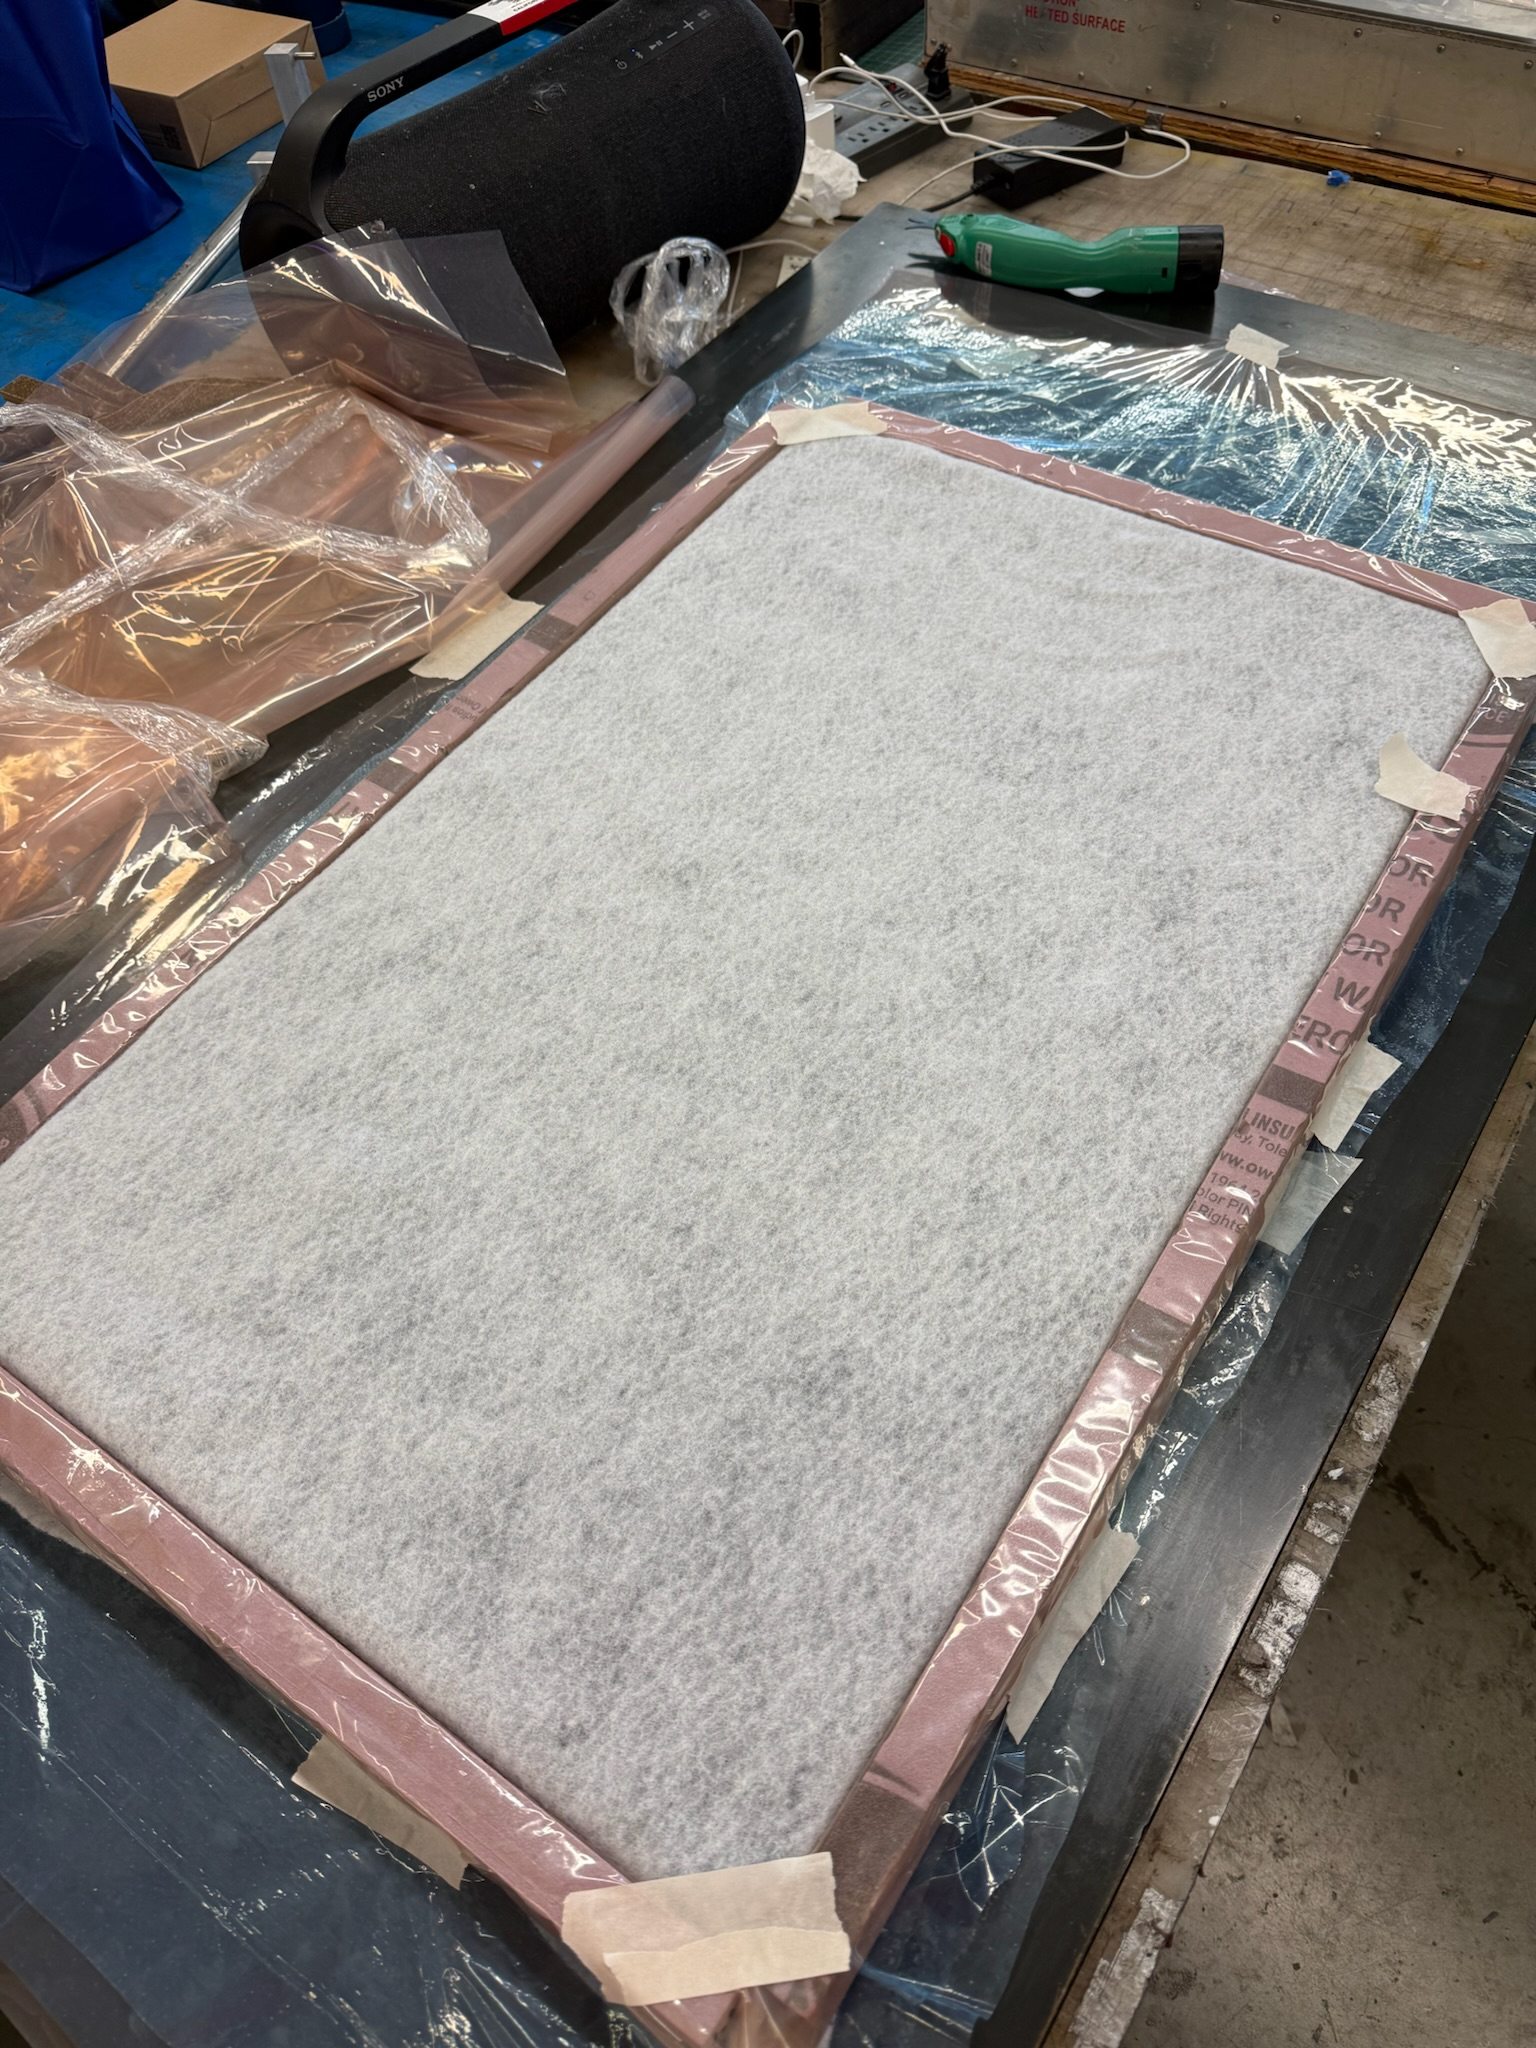
\includegraphics[
        width=3.10in,
        height=1.40in,
        keepaspectratio
    ]{completed_layup}
};
\draw[RuleGray,line width=0.55pt,rounded corners=4pt]
    ($(current page.north west)+(0.43in,-5.13in)$)
    rectangle
    ($(current page.north west)+(3.71in,-6.62in)$);

% Row 2 image 2 — oven chamber used only as a reliable vacuum enclosure; no heat applied
\node[anchor=center,inner sep=0pt]
at ($(current page.north west)+(5.50in,-5.875in)$)
{
    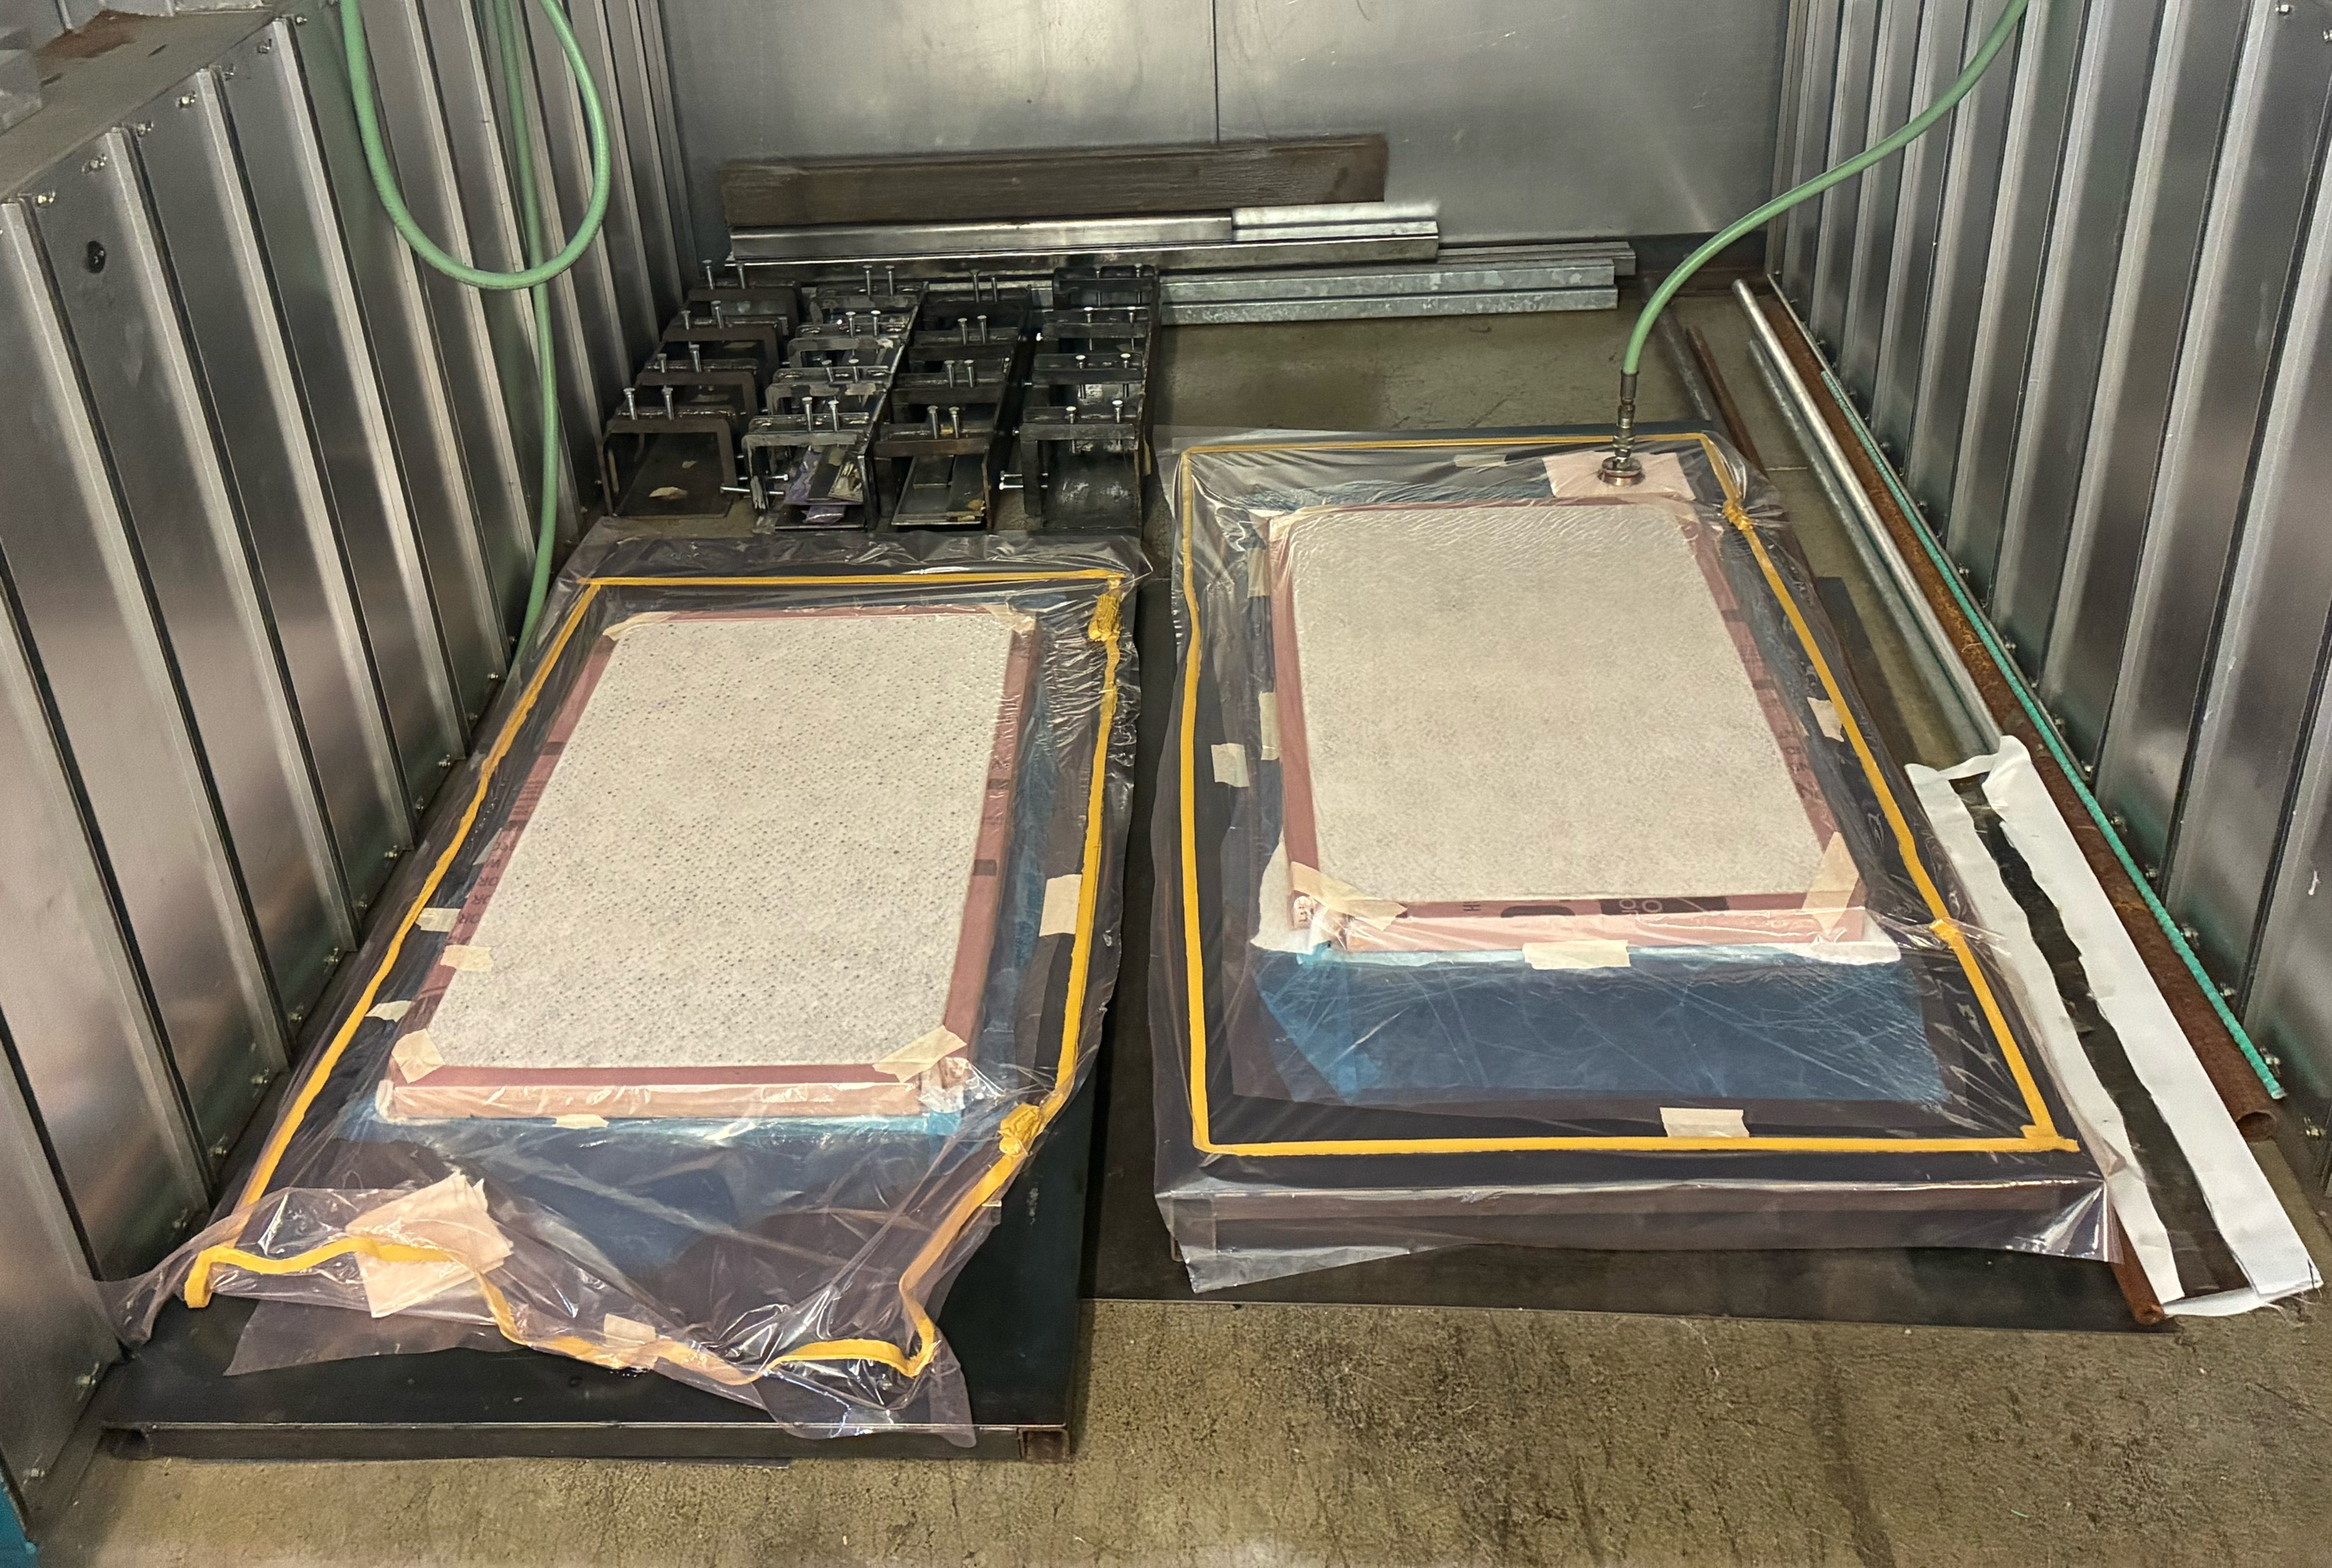
\includegraphics[
        width=3.10in,
        height=1.40in,
        keepaspectratio
    ]{layups_in_composite_oven_under_vacuumPressure}
};
\draw[RuleGray,line width=0.55pt,rounded corners=4pt]
    ($(current page.north west)+(3.86in,-5.13in)$)
    rectangle
    ($(current page.north west)+(7.14in,-6.62in)$);

% Row 2 image 3
\node[anchor=center,inner sep=0pt]
at ($(current page.north west)+(8.935in,-5.875in)$)
{
    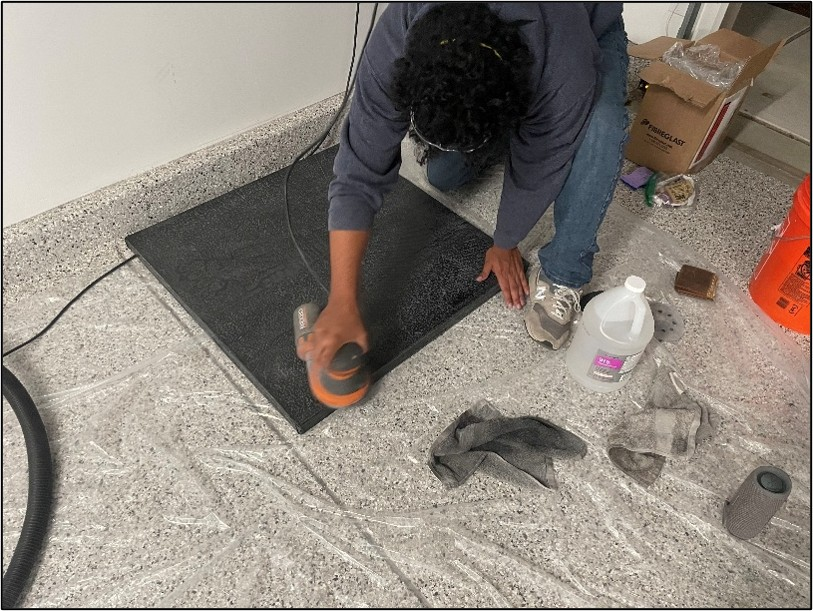
\includegraphics[
        width=3.10in,
        height=1.40in,
        keepaspectratio
    ]{garage_sanding}
};
\draw[RuleGray,line width=0.55pt,rounded corners=4pt]
    ($(current page.north west)+(7.29in,-5.13in)$)
    rectangle
    ($(current page.north east)+(-0.42in,-6.62in)$);

% Row 2 captions
\node[anchor=north,text=Muted,font=\sffamily\fontsize{6.7}{7.3}\selectfont]
at ($(current page.north west)+(2.07in,-6.67in)$)
{4. Fully saturated carbon skin and foam sandwich};

\node[anchor=north,text=Muted,font=\sffamily\fontsize{6.7}{7.3}\selectfont]
at ($(current page.north west)+(5.50in,-6.67in)$)
{5. Room-temperature cure under continuous vacuum};

\node[anchor=north,text=Muted,font=\sffamily\fontsize{6.7}{7.3}\selectfont]
at ($(current page.north west)+(8.935in,-6.67in)$)
{6. Post-processing and surface preparation};

% Bottom callouts
\fill[Panel,rounded corners=4pt]
    ($(current page.north west)+(0.43in,-6.95in)$)
    rectangle
    ($(current page.north west)+(5.48in,-7.60in)$);

\draw[RuleGray,line width=0.55pt,rounded corners=4pt]
    ($(current page.north west)+(0.43in,-6.95in)$)
    rectangle
    ($(current page.north west)+(5.48in,-7.60in)$);

\node[
    anchor=north west,
    text=DeepGreen,
    font=\sffamily\bfseries\fontsize{7.0}{7.6}\selectfont
]
at ($(current page.north west)+(0.63in,-7.08in)$)
{FROM THREE LAYUPS TO ONE};

\node[
    anchor=north west,
    align=left,
    text width=4.56in,
    text=Ink,
    font=\fontsize{6.45}{7.45}\selectfont
]
at ($(current page.north west)+(0.63in,-7.29in)$)
{
The Envelope Method reduced labor, cure cycles, handling,
alignment risk, and time spent forming numerous vacuum-bag
pleats around the 1.5-inch-thick XPS panels.
};

\fill[Panel,rounded corners=4pt]
    ($(current page.north west)+(5.68in,-6.95in)$)
    rectangle
    ($(current page.north east)+(-0.42in,-7.60in)$);

\draw[RuleGray,line width=0.55pt,rounded corners=4pt]
    ($(current page.north west)+(5.68in,-6.95in)$)
    rectangle
    ($(current page.north east)+(-0.42in,-7.60in)$);

\node[
    anchor=north west,
    text=DeepGreen,
    font=\sffamily\bfseries\fontsize{7.0}{7.6}\selectfont
]
at ($(current page.north west)+(5.88in,-7.08in)$)
{WHY SURFACE-BONDED HARDWARE};

\node[
    anchor=north west,
    align=left,
    text width=4.55in,
    text=Ink,
    font=\fontsize{6.45}{7.45}\selectfont
]
at ($(current page.north west)+(5.88in,-7.29in)$)
{
Adhesively bonded hinges and fixtures preserved the clean
composite exterior and avoided drilled inserts, foam-core
crushing, added stress concentrations, and new leak paths.
};


% Footer
\node[
    anchor=south west,
    text=white,
    font=\sffamily\bfseries\fontsize{7.1}{7.7}\selectfont
]
at ($(current page.south west)+(0.42in,0.17in)$)
{\faArrowLeft\ PRODUCT ARCHITECTURE};

\node[
    anchor=south,
    text=white,
    font=\sffamily\fontsize{7.0}{7.6}\selectfont
]
at ($(current page.south)+(0,0.17in)$)
{TORO COVER \hspace{6pt} 2 / 3};

\node[
    anchor=south east,
    text=white,
    font=\sffamily\bfseries\fontsize{7.1}{7.7}\selectfont
]
at ($(current page.south east)+(-0.42in,0.17in)$)
{VALIDATION \& TAKEAWAYS \faArrowRight};

\end{tikzpicture}


% ============================================================
% PAGE 3 — FINISHING, VALIDATION, AND TAKEAWAYS
% ============================================================

\clearpage
\thispagestyle{empty}
\hypertarget{toro-results}{}
\null

\begin{tikzpicture}[remember picture,overlay]

% Background and bars
\fill[white]
    (current page.south west)
    rectangle
    (current page.north east);

\fill[DeepGreen]
    (current page.north west)
    rectangle
    ($(current page.north east)+(0,-0.095in)$);

\fill[PolyGold]
    ($(current page.north west)+(0,-0.095in)$)
    rectangle
    ($(current page.north east)+(0,-0.14in)$);

\fill[DeepGreen]
    (current page.south west)
    rectangle
    ($(current page.south east)+(0,0.36in)$);

\fill[PolyGold]
    ($(current page.south west)+(0,0.36in)$)
    rectangle
    ($(current page.south east)+(0,0.405in)$);

% Header
\node[
    anchor=north west,
    text=PolyGold,
    font=\sffamily\bfseries\fontsize{8.1}{8.7}\selectfont
]
at ($(current page.north west)+(0.42in,-0.39in)$)
{TORO COVER \hspace{5pt}/\hspace{5pt} VALIDATION AND ENGINEERING TAKEAWAYS};

\node[
    anchor=north west,
    text=DeepGreen,
    font=\bfseries\fontsize{22.5}{23.5}\selectfont
]
at ($(current page.north west)+(0.40in,-0.67in)$)
{FROM PROTOTYPE TO PRODUCT PATHWAY};

\node[
    anchor=north west,
    text=Muted,
    font=\sffamily\fontsize{8.7}{9.6}\selectfont
]
at ($(current page.north west)+(0.42in,-1.12in)$)
{Environmental protection, usability testing, scope decisions, and lessons from technical leadership};

\fill[PolyGold]
    ($(current page.north west)+(0.42in,-1.36in)$)
    rectangle
    ($(current page.north west)+(5.8in,-1.315in)$);

% Finishing title
\node[
    anchor=north west,
    text=DeepGreen,
    font=\sffamily\bfseries\fontsize{8.0}{8.7}\selectfont
]
at ($(current page.north west)+(0.43in,-1.62in)$)
{OUTDOOR FINISHING AND ENVIRONMENTAL PROTECTION};

% Image 1
\node[anchor=center,inner sep=0pt]
at ($(current page.north west)+(1.705in,-2.655in)$)
{
    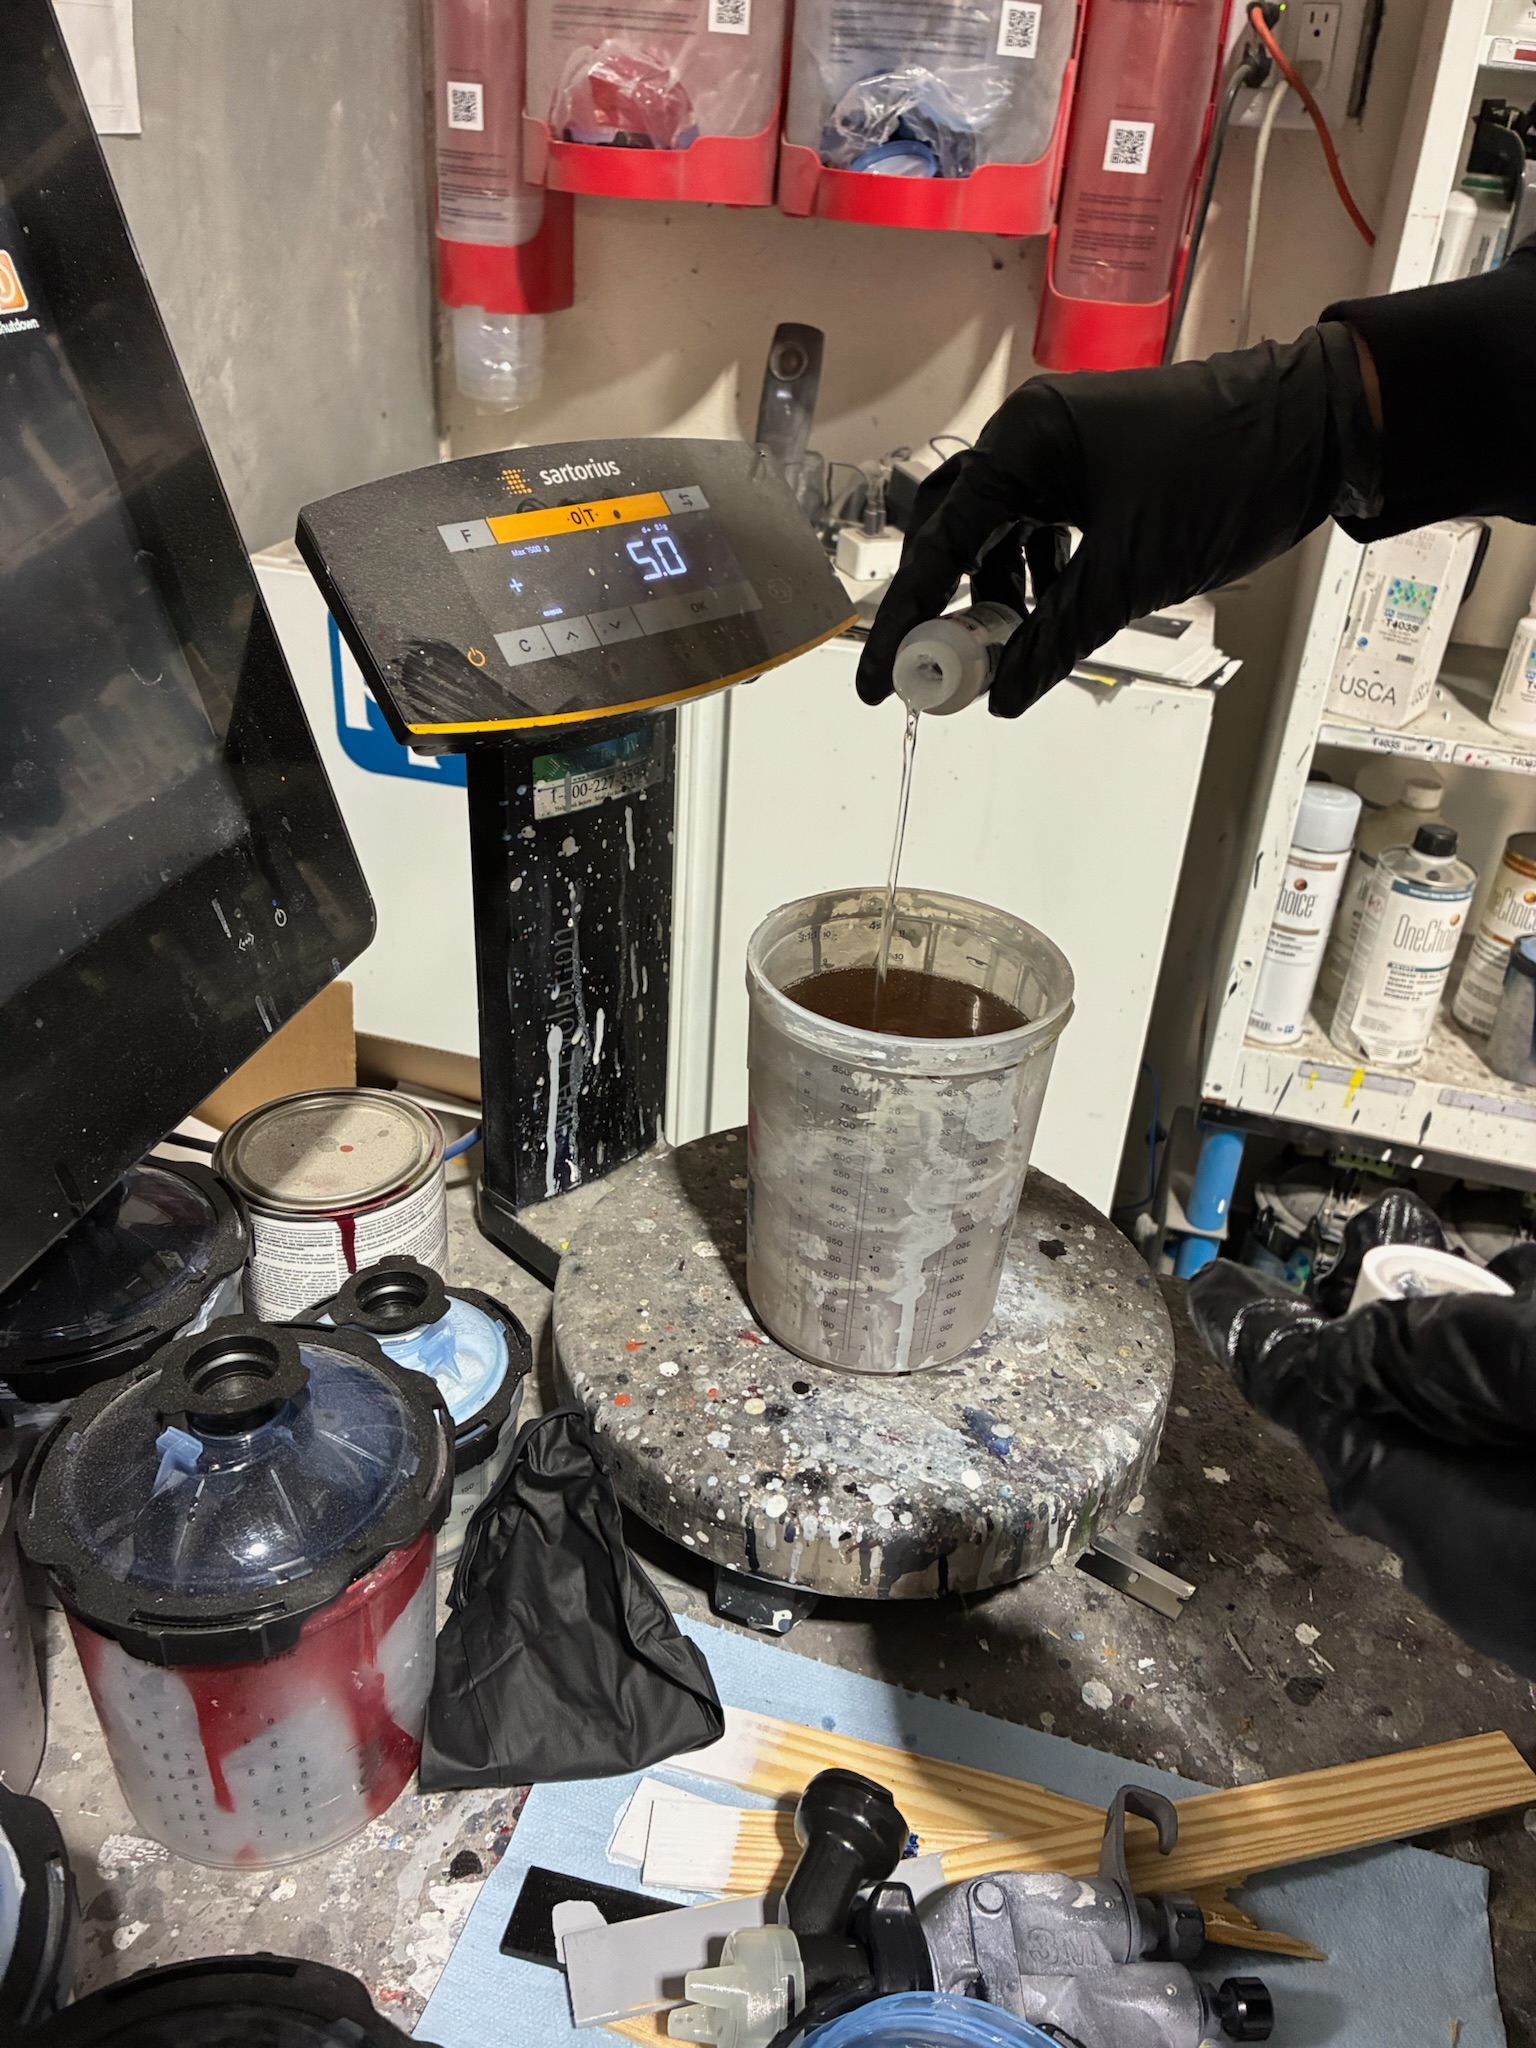
\includegraphics[
        width=2.35in,
        height=1.40in,
        keepaspectratio
    ]{spray_topcoat_prep}
};
\draw[RuleGray,line width=0.55pt,rounded corners=4pt]
    ($(current page.north west)+(0.43in,-1.91in)$)
    rectangle
    ($(current page.north west)+(2.98in,-3.40in)$);

% Image 2
\node[anchor=center,inner sep=0pt]
at ($(current page.north west)+(4.375in,-2.655in)$)
{
    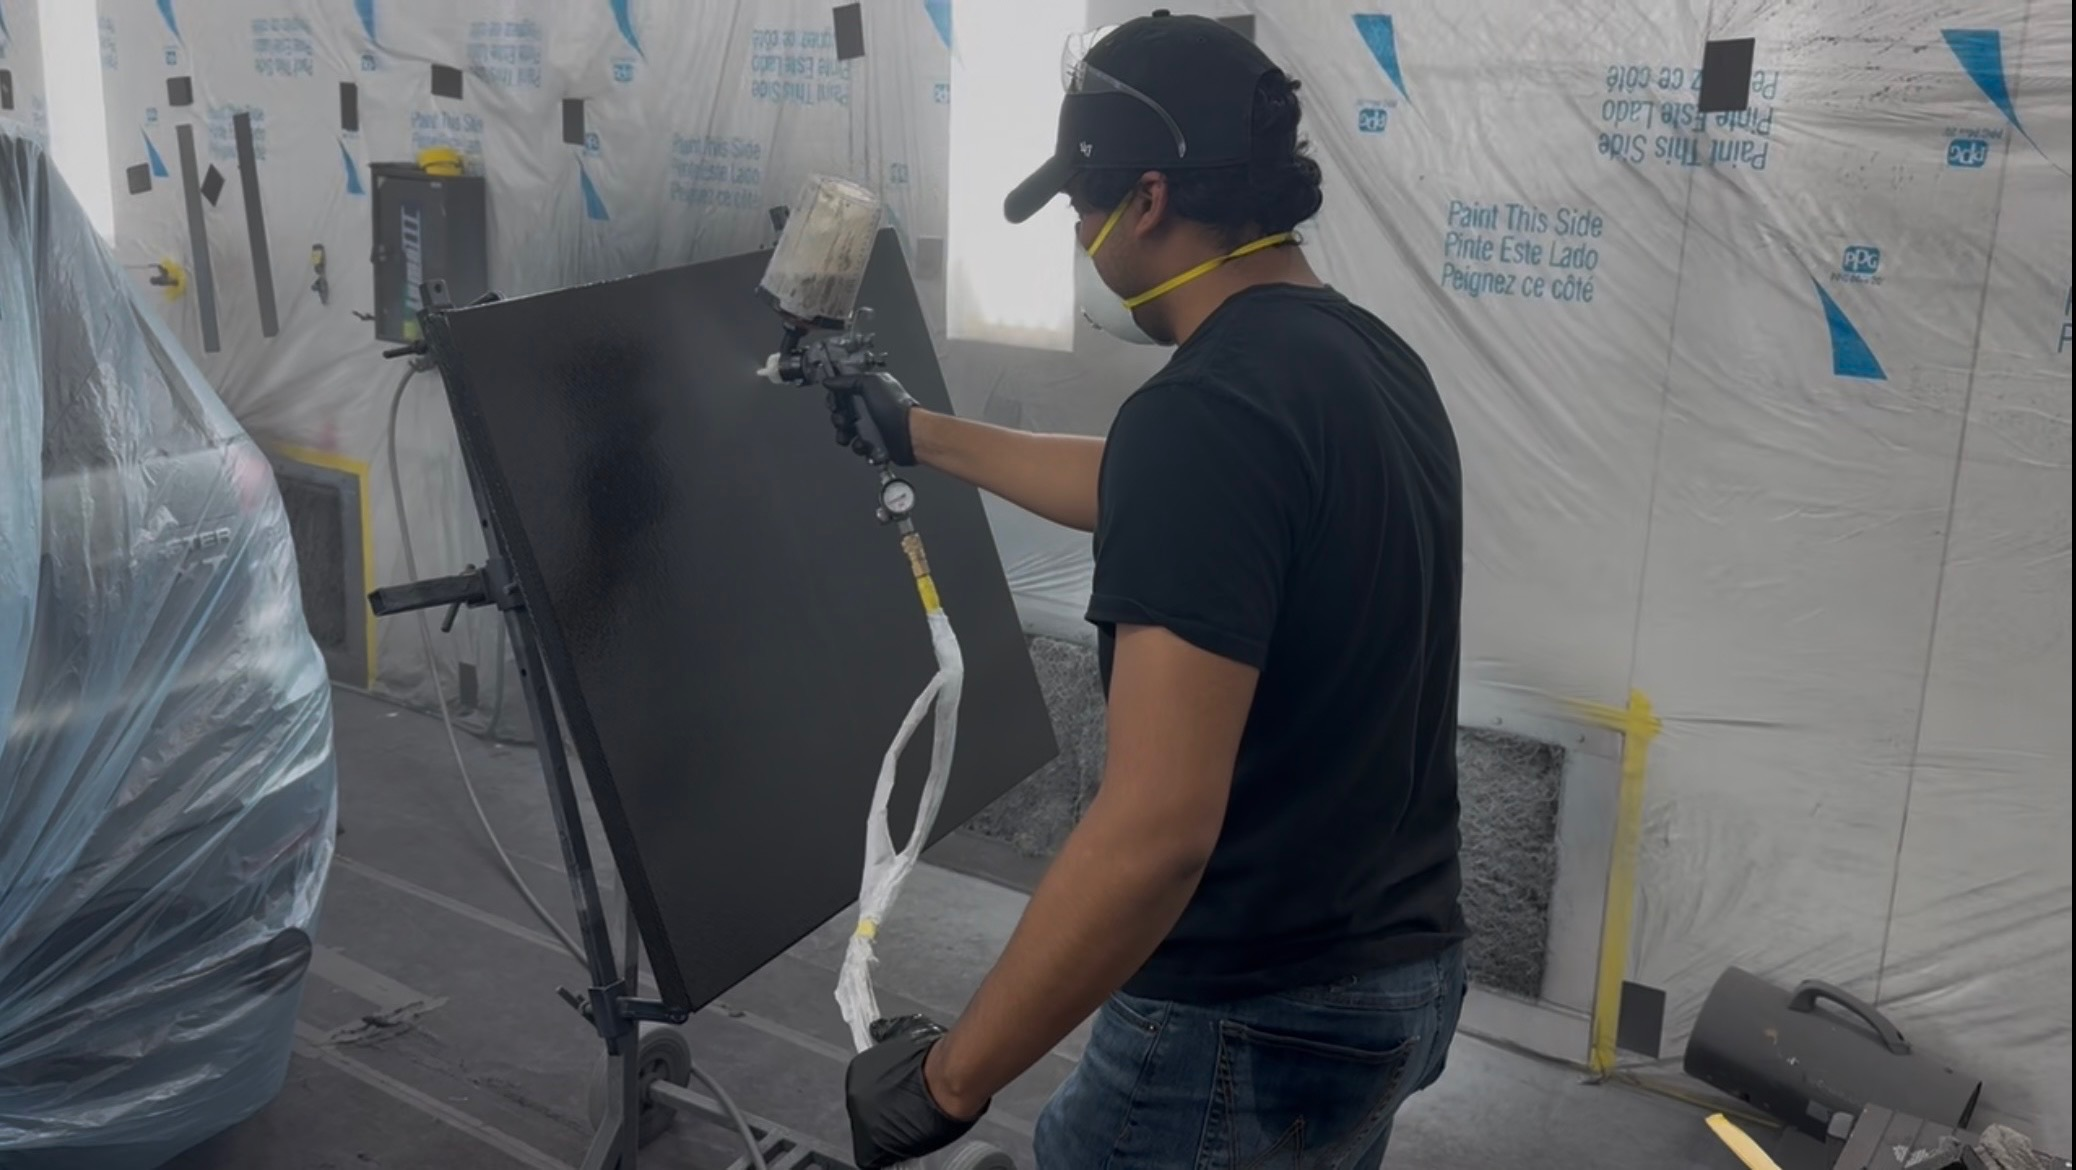
\includegraphics[
        width=2.35in,
        height=1.40in,
        keepaspectratio
    ]{spraying_topcoat}
};
\draw[RuleGray,line width=0.55pt,rounded corners=4pt]
    ($(current page.north west)+(3.10in,-1.91in)$)
    rectangle
    ($(current page.north west)+(5.65in,-3.40in)$);

% Image 3
\node[anchor=center,inner sep=0pt]
at ($(current page.north west)+(7.045in,-2.655in)$)
{
    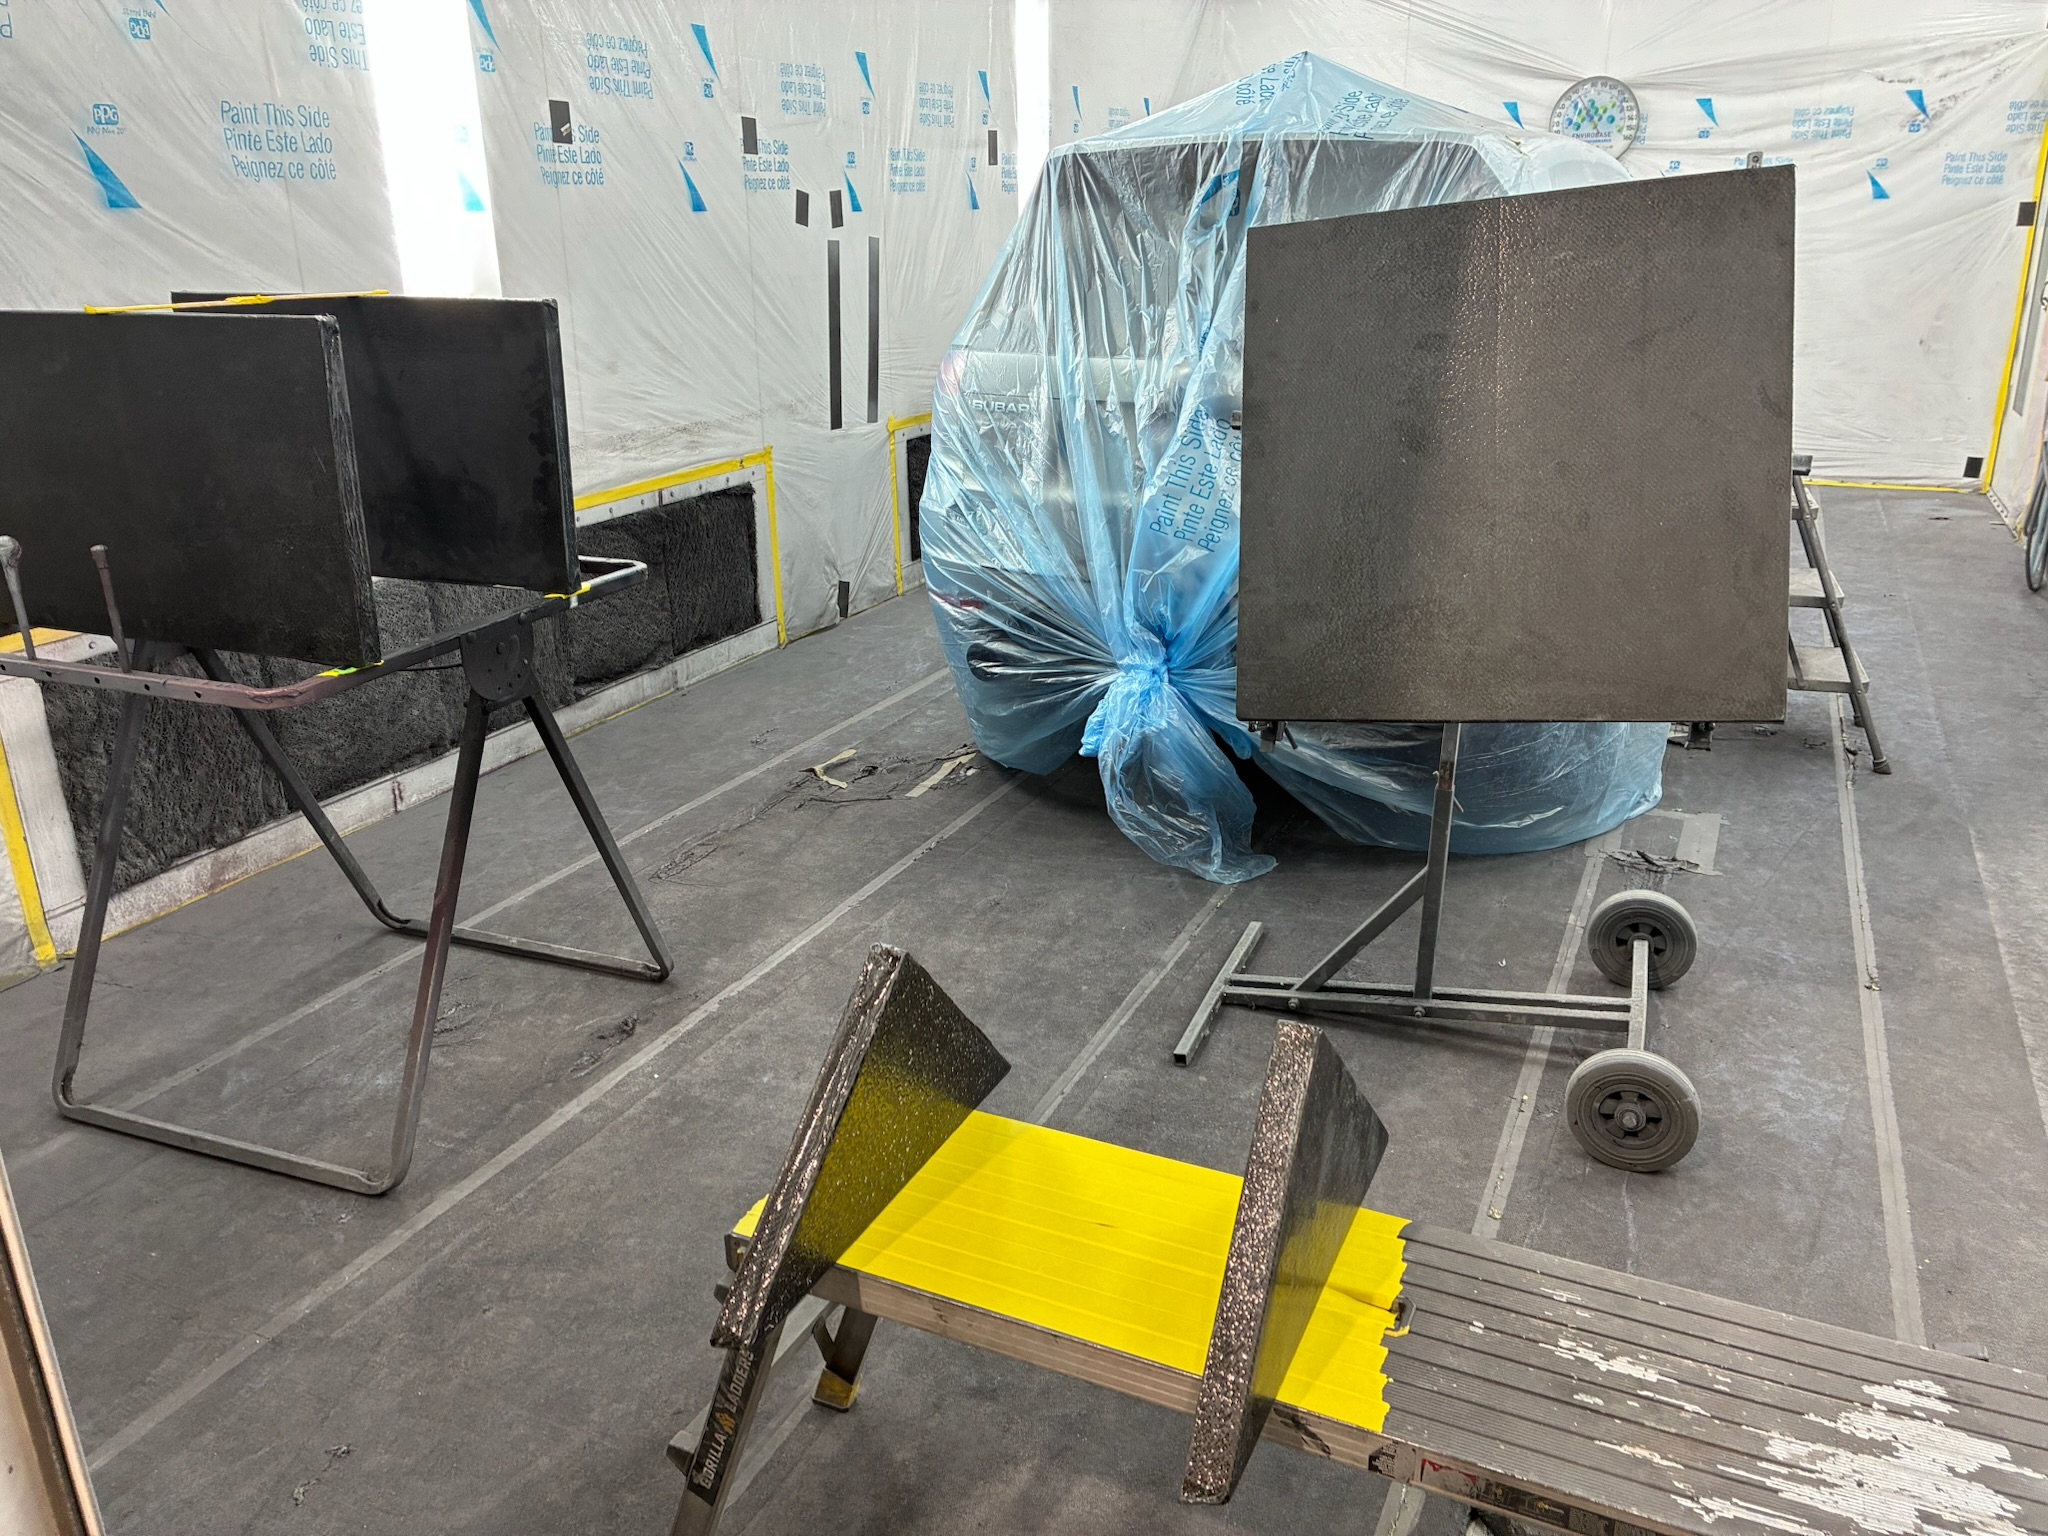
\includegraphics[
        width=2.35in,
        height=1.40in,
        keepaspectratio
    ]{topcoat_setup_apparatus}
};
\draw[RuleGray,line width=0.55pt,rounded corners=4pt]
    ($(current page.north west)+(5.77in,-1.91in)$)
    rectangle
    ($(current page.north west)+(8.32in,-3.40in)$);

% Image 4
\node[anchor=center,inner sep=0pt]
at ($(current page.north west)+(9.50in,-2.655in)$)
{
    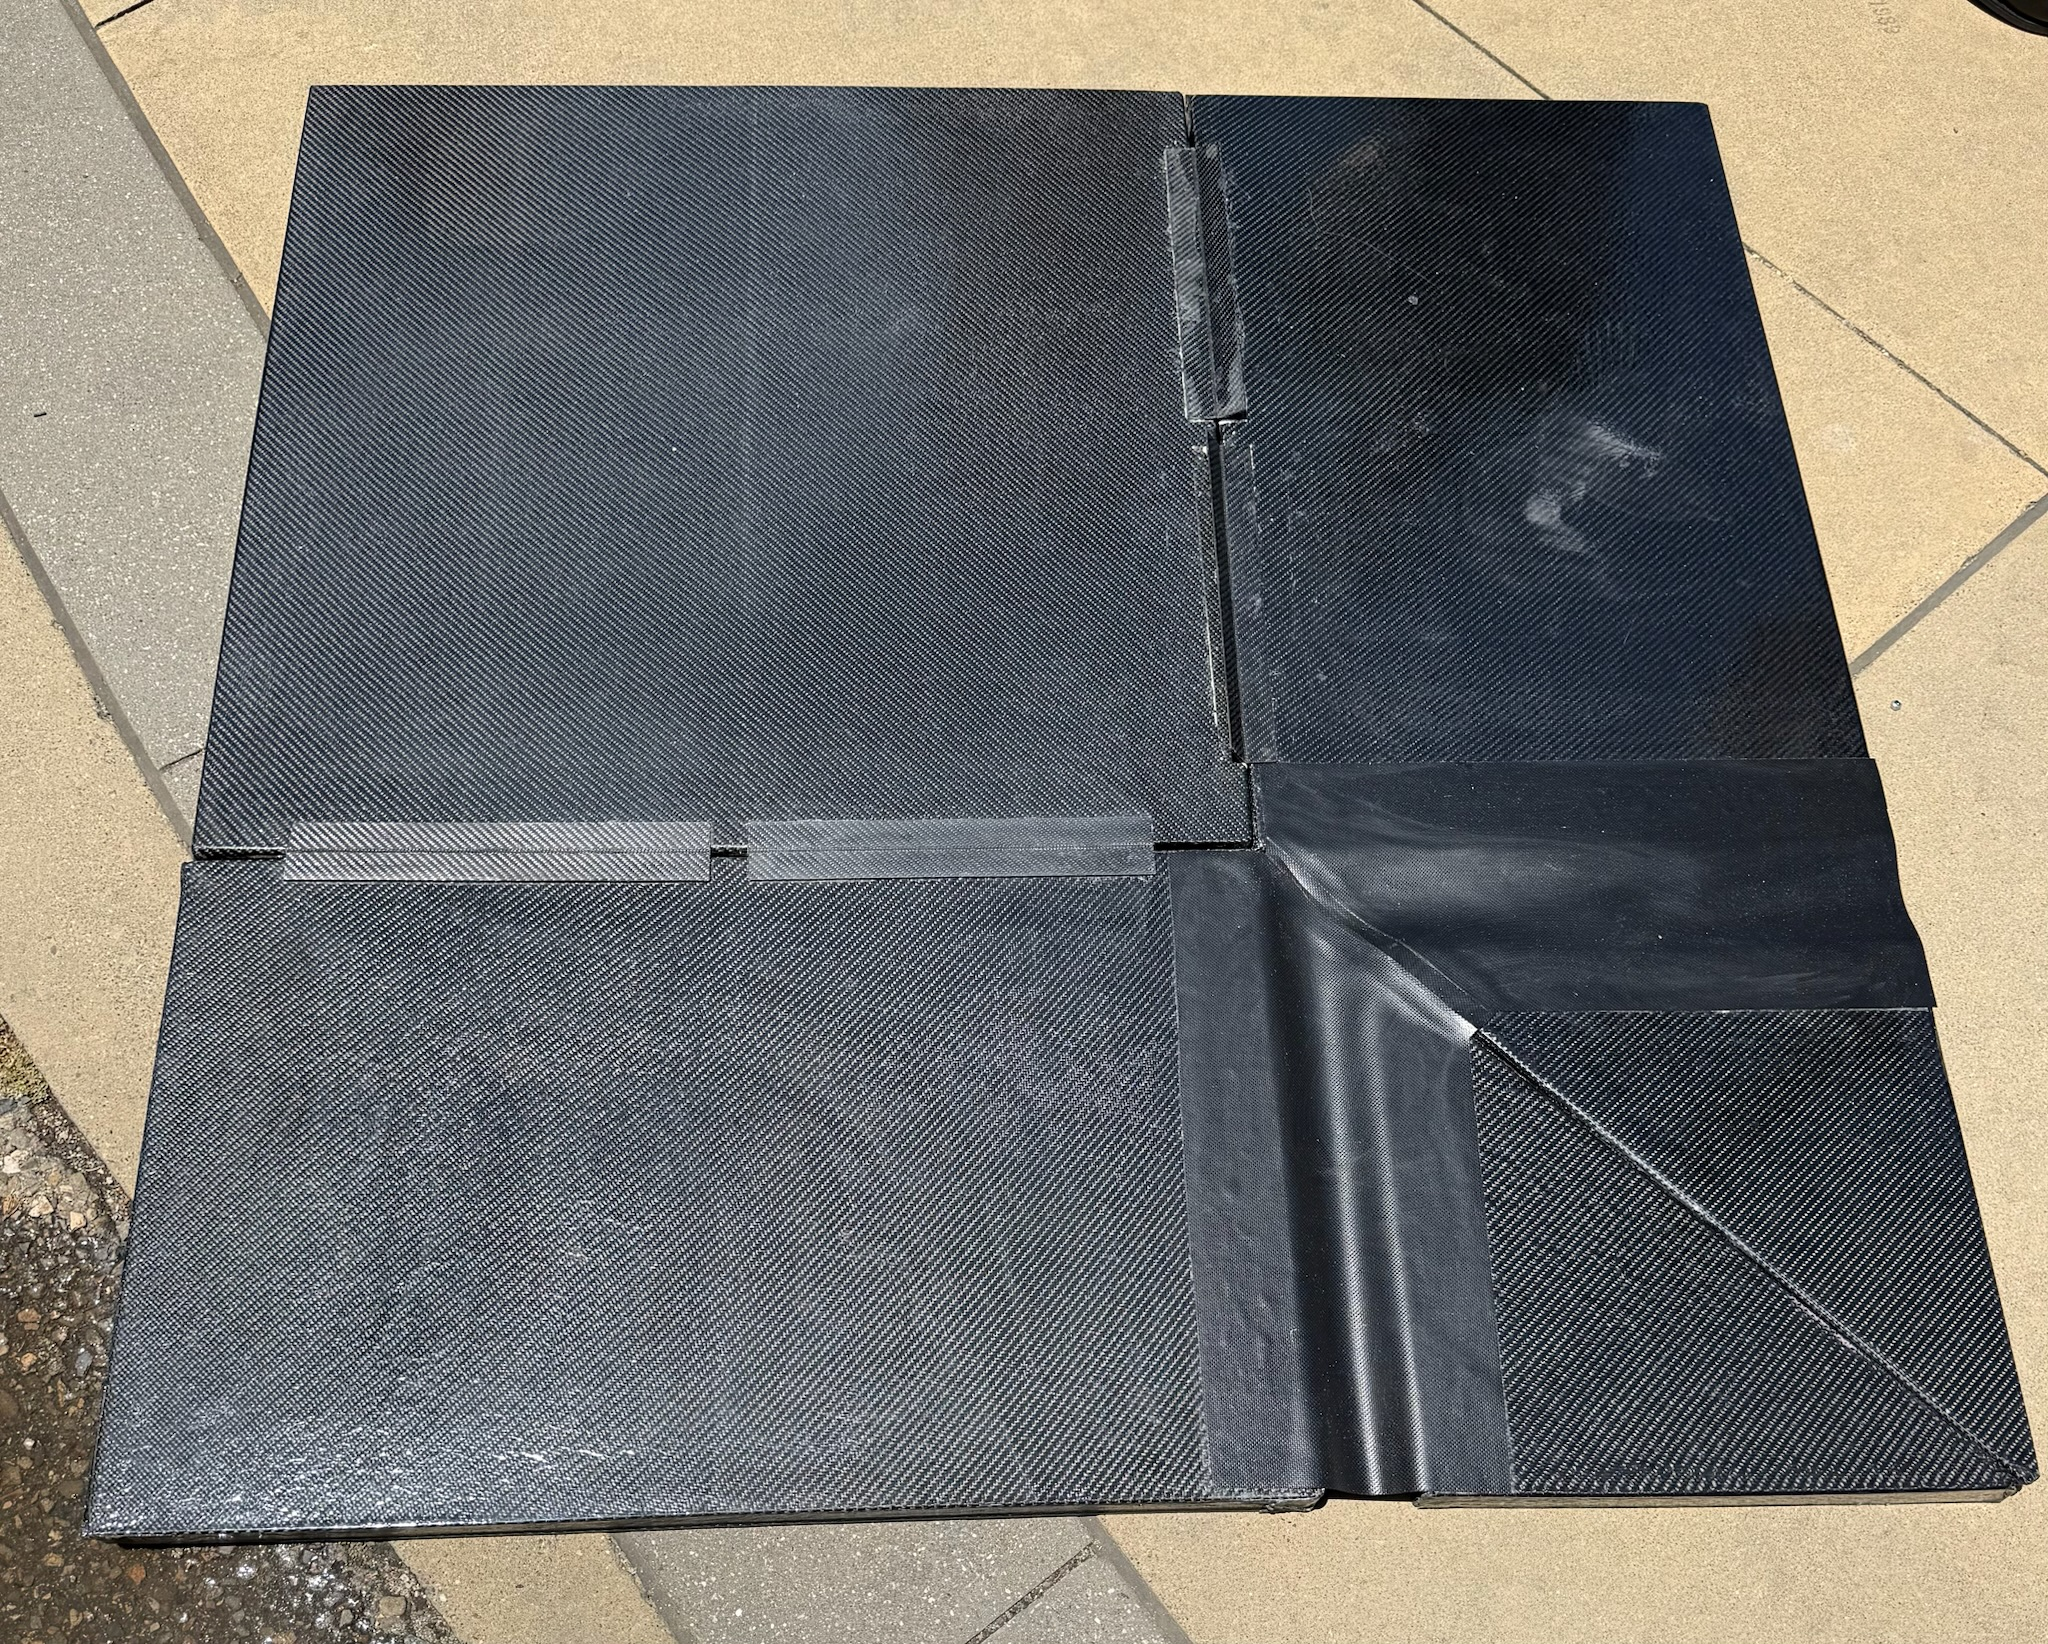
\includegraphics[
        width=2.35in,
        height=1.40in,
        keepaspectratio
    ]{refined_final_toro_cover_partial_carbon_model}
};
\draw[RuleGray,line width=0.55pt,rounded corners=4pt]
    ($(current page.north west)+(8.44in,-1.91in)$)
    rectangle
    ($(current page.north east)+(-0.42in,-3.40in)$);

% Captions
\node[anchor=north,text=Muted,font=\sffamily\fontsize{6.7}{7.3}\selectfont]
at ($(current page.north west)+(1.705in,-3.45in)$)
{Topcoat material preparation};

\node[anchor=north,text=Muted,font=\sffamily\fontsize{6.7}{7.3}\selectfont]
at ($(current page.north west)+(4.375in,-3.45in)$)
{Automotive-booth topcoat application};

\node[anchor=north,text=Muted,font=\sffamily\fontsize{6.7}{7.3}\selectfont]
at ($(current page.north west)+(7.045in,-3.45in)$)
{Coated panels drying after application};

\node[anchor=north,text=Muted,font=\sffamily\fontsize{6.7}{7.3}\selectfont]
at ($(current page.north west)+(9.50in,-3.45in)$)
{Partial carbon manufacturing model};

% Environmental rationale
\fill[SoftGold,rounded corners=4pt]
    ($(current page.north west)+(0.43in,-3.73in)$)
    rectangle
    ($(current page.north east)+(-0.42in,-4.76in)$);

\node[
    anchor=north west,
    align=left,
    text width=9.75in,
    text=Ink,
    font=\fontsize{7.05}{8.25}\selectfont
]
at ($(current page.north west)+(0.65in,-3.89in)$)
{
Because the sponsor required a carbon-fiber cover for outdoor use near chlorinated water,
environmental protection became a functional requirement rather than a cosmetic finish.
I selected and personally sprayed a UV-resistant Sunshield topcoat to seal minor laminate
porosity, reduce moisture ingress, preserve the carbon appearance, limit UV degradation of
the epoxy matrix, and isolate the composite surface from nearby metallic hardware.
};

% Results title
\node[
    anchor=north west,
    text=DeepGreen,
    font=\sffamily\bfseries\fontsize{8.0}{8.7}\selectfont
]
at ($(current page.north west)+(0.43in,-4.94in)$)
{FUNCTIONAL PROTOTYPE RESULTS};

% ------------------------------------------------------------
% Matched lower panels — larger type and improved allocation
% ------------------------------------------------------------

% Left results panel
\fill[SoftGreen,rounded corners=5pt]
    ($(current page.north west)+(0.43in,-5.22in)$)
    rectangle
    ($(current page.north west)+(5.98in,-7.39in)$);

\draw[RuleGray,line width=0.65pt,rounded corners=5pt]
    ($(current page.north west)+(0.43in,-5.22in)$)
    rectangle
    ($(current page.north west)+(5.98in,-7.39in)$);

\fill[DeepGreen,rounded corners=5pt]
    ($(current page.north west)+(0.43in,-5.22in)$)
    rectangle
    ($(current page.north west)+(5.98in,-5.58in)$);

\fill[DeepGreen]
    ($(current page.north west)+(0.43in,-5.40in)$)
    rectangle
    ($(current page.north west)+(5.98in,-5.58in)$);

\node[anchor=west,text=white,
      font=\sffamily\bfseries\fontsize{7.0}{7.6}\selectfont]
at ($(current page.north west)+(0.66in,-5.40in)$)
{SPECIFICATION};

\node[anchor=west,text=white,
      font=\sffamily\bfseries\fontsize{7.0}{7.6}\selectfont]
at ($(current page.north west)+(3.02in,-5.40in)$)
{RESULT};

\node[anchor=east,text=white,
      font=\sffamily\bfseries\fontsize{7.0}{7.6}\selectfont]
at ($(current page.north west)+(5.55in,-5.40in)$)
{STATUS};

\node[
    anchor=north west,
    align=left,
    text width=2.15in,
    text=Ink,
    font=\bfseries\fontsize{7.15}{8.55}\selectfont
]
at ($(current page.north west)+(0.66in,-5.72in)$)
{
Deployment time\\[3.4pt]
Removal time\\[3.4pt]
Single-user operation\\[3.4pt]
Single-side operation\\[3.4pt]
Deployment steps\\[3.4pt]
Removal steps\\[3.4pt]
Weight\\[3.4pt]
Folded storage
};

\node[
    anchor=north west,
    align=left,
    text width=1.45in,
    text=Ink,
    font=\fontsize{7.15}{8.55}\selectfont
]
at ($(current page.north west)+(3.02in,-5.72in)$)
{
25.51 seconds\\[3.4pt]
37.22 seconds\\[3.4pt]
100\% successful\\[3.4pt]
75\% successful\\[3.4pt]
6.4 average\\[3.4pt]
9 average\\[3.4pt]
17 lb\\[3.4pt]
2.9' x 2.9' x 1.7'
};

\node[
    anchor=north east,
    align=right,
    text width=1.05in,
    text=DeepGreen,
    font=\sffamily\bfseries\fontsize{7.05}{8.55}\selectfont
]
at ($(current page.north west)+(5.55in,-5.72in)$)
{
PASS\\[3.4pt]
PASS\\[3.4pt]
PASS\\[3.4pt]
NEAR TARGET\\[3.4pt]
PASS\\[3.4pt]
PASS\\[3.4pt]
NEAR TARGET\\[3.4pt]
PASS
};

% Right takeaways panel — widened for easier reading
\fill[SoftGreen,rounded corners=5pt]
    ($(current page.north west)+(6.14in,-5.22in)$)
    rectangle
    ($(current page.north east)+(-0.42in,-7.39in)$);

\draw[RuleGray,line width=0.65pt,rounded corners=5pt]
    ($(current page.north west)+(6.14in,-5.22in)$)
    rectangle
    ($(current page.north east)+(-0.42in,-7.39in)$);

\fill[DeepGreen,rounded corners=5pt]
    ($(current page.north west)+(6.14in,-5.22in)$)
    rectangle
    ($(current page.north east)+(-0.42in,-5.58in)$);

\fill[DeepGreen]
    ($(current page.north west)+(6.14in,-5.40in)$)
    rectangle
    ($(current page.north east)+(-0.42in,-5.58in)$);

\node[anchor=west,text=white,
      font=\sffamily\bfseries\fontsize{7.1}{7.7}\selectfont]
at ($(current page.north west)+(6.38in,-5.40in)$)
{ENGINEERING TAKEAWAYS};

\node[
    anchor=north west,
    align=left,
    text width=4.02in,
    text=Ink,
    font=\fontsize{6.75}{7.85}\selectfont
]
at ($(current page.north west)+(6.38in,-5.72in)$)
{
\textbf{Manufacturing first.}
Composite manufacturing constraints should guide the product architecture from the beginning.\\[4.5pt]
\textbf{Prioritize deliberately.}
Competing requirements must be balanced intentionally instead of maximizing every objective.\\[4.5pt]
\textbf{Lead through the process.}
Clear procedures, calm communication, and respect for teammates' strengths were essential during fabrication.\\[4.5pt]
\textbf{Next iteration.}
Reduce weight, refine the fabric-hinge fold lines, and improve panel-edge clearance.
};

% Compact concluding pathway
\node[
    anchor=center,
    align=center,
    text=PolyGold,
    font=\sffamily\bfseries\fontsize{6.3}{6.9}\selectfont
]
at ($(current page.north)+(3.06in,-7.18in)$)
{PROTOTYPE \faArrowRight\ DESIGN REFINEMENT
\faArrowRight\ REPEATABLE MANUFACTURING
\faArrowRight\ PRODUCT};

% Validation resources
\node[
    anchor=north,
    align=center,
    text=DeepGreen,
    font=\sffamily\bfseries\fontsize{6.6}{7.2}\selectfont
]
at ($(current page.north)+(0,-7.58in)$)
{\href{\ToroDeploymentLink}{\faPlayCircle\ DEPLOYMENT}
\hspace{18pt}
\href{\ToroRemovalLink}{\faPlayCircle\ REMOVAL / FOLDING}
\hspace{18pt}
\href{\ToroPosterLink}{\faFilePdf\ EXPO POSTER}
\hspace{18pt}
\href{\ToroReportLink}{\faFilePdf\ FINAL REPORT}};

% Footer
\node[
    anchor=south west,
    text=white,
    font=\sffamily\bfseries\fontsize{7.1}{7.7}\selectfont
]
at ($(current page.south west)+(0.42in,0.17in)$)
{\faArrowLeft\ MANUFACTURING-DRIVEN DESIGN};

\node[
    anchor=south,
    text=white,
    font=\sffamily\fontsize{7.0}{7.6}\selectfont
]
at ($(current page.south)+(0,0.17in)$)
{TORO COVER \hspace{6pt} 3 / 3};

\node[
    anchor=south east,
    text=white,
    font=\sffamily\bfseries\fontsize{7.1}{7.7}\selectfont
]
at ($(current page.south east)+(-0.42in,0.17in)$)
{NEXT PROJECT \faArrowRight};

\end{tikzpicture}
\input{paddle}
\clearpage
.
% 2. In main.tex, place 
% ============================================================
% TORO COVER — THREE-PAGE PORTFOLIO CASE STUDY
% Pages 3–5 of the complete portfolio
%
% IMPORTANT:
% 1. This file must NOT contain \documentclass, \begin{document},
%    \end{document}, or \input{toro}.
% 2. In main.tex, place \input{toro} before \end{document}.
% 3. Image references use the original Overleaf base filenames
%    without extensions.
% ============================================================



% ============================================================
% CLICKABLE PROJECT RESOURCES
% All links use the exact Google Drive resources supplied.
% ============================================================
\providecommand{\ToroDrawingLink}{https://drive.google.com/file/d/1A7-7wMnRNLuQDaTgxeuUCBsGNqyXzOGV/view?usp=sharing}
\providecommand{\ToroDimensionsLink}{https://drive.google.com/file/d/13sw3BNJvE8GdzlRffxoF2n5r9Gzxide7/view?usp=sharing}
\providecommand{\ToroProblemLink}{https://drive.google.com/file/d/1zHtl8zrb13F1yeN74ptawpfS5UM_xsuw/view?usp=drive_link}
\providecommand{\ToroReportLink}{https://drive.google.com/file/d/1ULZ-P46lFsC2x29ZfmRVIKgYnr9o8hMt/view?usp=drive_link}
\providecommand{\ToroPosterLink}{https://drive.google.com/file/d/1vKiKaJUcHQb_db-FkZnRF6EvtuM4hKyS/view?usp=drive_link}
\providecommand{\ToroDeploymentLink}{https://drive.google.com/file/d/1XJx34o80_mZPTl7xy93HtWAgtS3ThhvY/view?usp=drive_link}
\providecommand{\ToroRemovalLink}{https://drive.google.com/file/d/1O7xYeyB67NUwT-j1B1HeiCcHnZDYjk6_/view?usp=drive_link}

% ============================================================
% PAGE 1 — PROJECT OVERVIEW, OWNERSHIP, AND ARCHITECTURE
% ============================================================

\clearpage
\thispagestyle{empty}
\hypertarget{toro}{}
\null

\begin{tikzpicture}[remember picture,overlay]

% Background
\fill[white]
    (current page.south west)
    rectangle
    (current page.north east);

% Page bars
\fill[DeepGreen]
    (current page.north west)
    rectangle
    ($(current page.north east)+(0,-0.095in)$);

\fill[PolyGold]
    ($(current page.north west)+(0,-0.095in)$)
    rectangle
    ($(current page.north east)+(0,-0.14in)$);

\fill[DeepGreen]
    (current page.south west)
    rectangle
    ($(current page.south east)+(0,0.36in)$);

\fill[PolyGold]
    ($(current page.south west)+(0,0.36in)$)
    rectangle
    ($(current page.south east)+(0,0.405in)$);

% Header
\node[
    anchor=north west,
    text=PolyGold,
    font=\sffamily\bfseries\fontsize{8.1}{8.7}\selectfont
]
at ($(current page.north west)+(0.42in,-0.39in)$)
{01 COMPOSITES \hspace{5pt}/\hspace{5pt} PROJECT 01};

\node[
    anchor=north west,
    text=DeepGreen,
    font=\bfseries\fontsize{23.5}{24.5}\selectfont
]
at ($(current page.north west)+(0.40in,-0.67in)$)
{TORO CARBON FIBER SAFETY COVER};

\node[
    anchor=north west,
    text=Muted,
    font=\sffamily\fontsize{8.4}{9.2}\selectfont
]
at ($(current page.north west)+(0.42in,-1.12in)$)
{Cal Poly Composites Laboratory \hspace{7pt}\textbullet\hspace{7pt}
Team Project \hspace{7pt}\textbullet\hspace{7pt}
Fall--Spring 2026 \hspace{7pt}\textbullet\hspace{7pt}
San Luis Obispo, California};

\fill[PolyGold]
    ($(current page.north west)+(0.42in,-1.37in)$)
    rectangle
    ($(current page.north west)+(6.1in,-1.325in)$);

% Challenge text
\node[
    anchor=north west,
    text=DeepGreen,
    font=\sffamily\bfseries\fontsize{8.1}{8.8}\selectfont
]
at ($(current page.north west)+(0.43in,-1.61in)$)
{THE CHALLENGE};

\node[
    anchor=north west,
    align=left,
    text width=4.47in,
    text=Ink,
    font=\fontsize{8.05}{9.65}\selectfont
]
at ($(current page.north west)+(0.43in,-1.84in)$)
{
Develop a lightweight cover for a 6 ft by 6 ft in-ground spa
that could be deployed by one person, stored compactly,
provide insulation, resist a poolside environment, and maintain
a refined appearance. The sponsor supplied an ambitious but
intentionally broad project statement, requiring the team to
define the product architecture, priorities, manufacturing
strategy, and realistic path toward future commercialization.
};

% Role box
\fill[SoftGold,rounded corners=5pt]
    ($(current page.north west)+(0.42in,-2.88in)$)
    rectangle
    ($(current page.north west)+(4.98in,-4.58in)$);

\fill[PolyGold]
    ($(current page.north west)+(0.42in,-2.88in)$)
    rectangle
    ($(current page.north west)+(0.52in,-4.58in)$);

\node[
    anchor=north west,
    text=DeepGreen,
    font=\sffamily\bfseries\fontsize{8.1}{8.8}\selectfont
]
at ($(current page.north west)+(0.66in,-3.02in)$)
{MY ROLE — DESIGN \& MANUFACTURING LEAD};

\node[
    anchor=north west,
    align=left,
    text width=4.02in,
    text=Ink,
    font=\fontsize{7.05}{8.15}\selectfont
]
at ($(current page.north west)+(0.66in,-3.27in)$)
{
\textbullet\ Modeled every custom part and the complete assembly\\[1.5pt]
\textbullet\ Produced the engineering drawing package independently\\[1.5pt]
\textbullet\ Developed the composite-panel manufacturing process\\[1.5pt]
\textbullet\ Created all waterjet DXFs and manufacturing geometry\\[1.5pt]
\textbullet\ Trained teammates in wet layup and vacuum bagging\\[1.5pt]
\textbullet\ Presented feasibility, scope, and tradeoffs to the sponsor
};

% Large deployed foam-model image
\node[anchor=center,inner sep=0pt]
at ($(current page.north west)+(8.00in,-3.04in)$)
{
    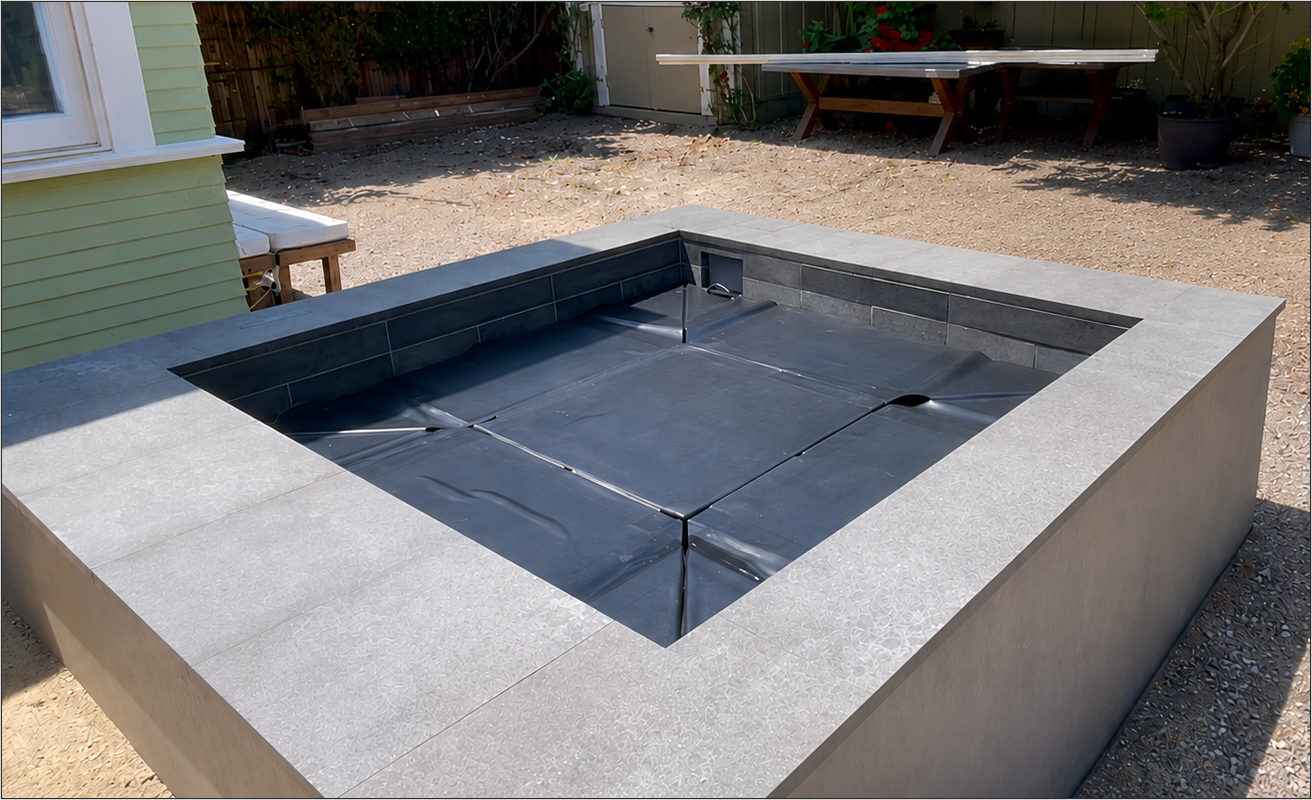
\includegraphics[
        width=5.55in,
        height=2.78in,
        keepaspectratio
    ]{deployed_functional_prototype}
};

\draw[DeepGreen,line width=0.8pt,rounded corners=7pt]
    ($(current page.north west)+(5.16in,-1.61in)$)
    rectangle
    ($(current page.north east)+(-0.42in,-4.47in)$);

\node[
    anchor=north west,
    text=Muted,
    font=\sffamily\fontsize{6.2}{6.9}\selectfont
]
at ($(current page.north west)+(5.18in,-4.54in)$)
{Functional foam model deployed over the sponsor's in-ground spa.};

% Image-strip title
\node[
    anchor=north west,
    text=DeepGreen,
    font=\sffamily\bfseries\fontsize{8.1}{8.8}\selectfont
]
at ($(current page.north west)+(0.43in,-4.78in)$)
{PRODUCT DEVELOPMENT AND FINAL ARCHITECTURE};

% Five-image development strip — CAD-first sequence
% Image 1: topside CAD
\node[anchor=center,inner sep=0pt]
at ($(current page.north west)+(1.47in,-5.73in)$)
{
    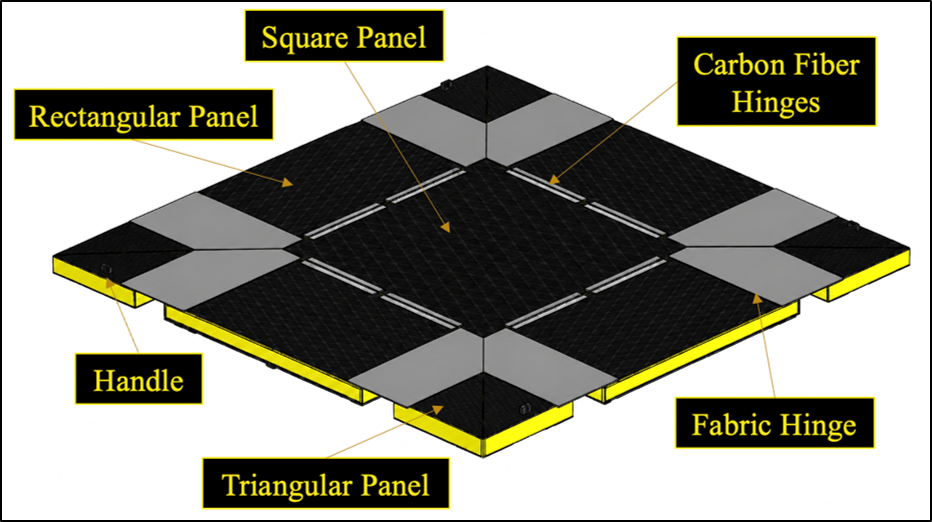
\includegraphics[
        width=1.92in,
        height=1.30in,
        keepaspectratio
    ]{Toro_Cover_topside_Cad}
};
\draw[RuleGray,line width=0.55pt,rounded corners=4pt]
    ($(current page.north west)+(0.43in,-5.04in)$)
    rectangle
    ($(current page.north west)+(2.51in,-6.43in)$);

% Image 2: underside CAD
\node[anchor=center,inner sep=0pt]
at ($(current page.north west)+(3.66in,-5.73in)$)
{
    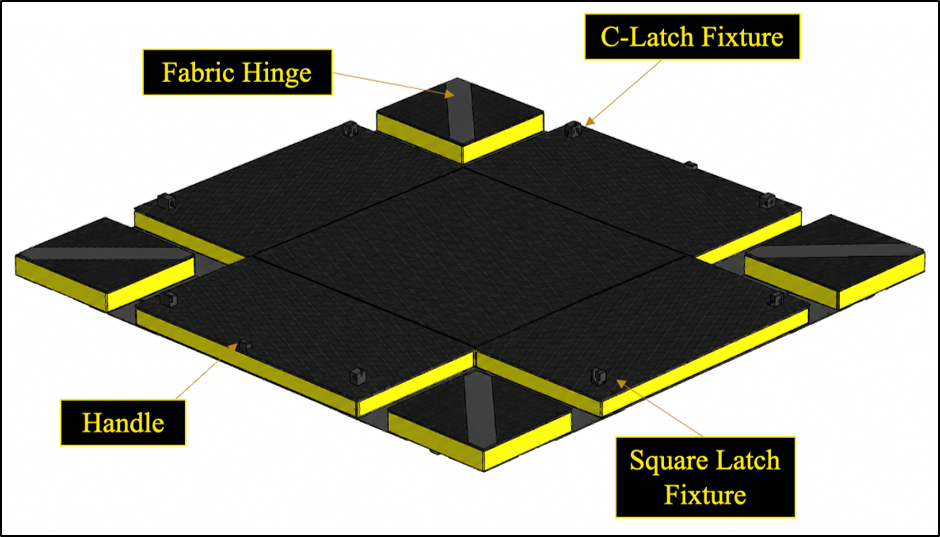
\includegraphics[
        width=1.92in,
        height=1.30in,
        keepaspectratio
    ]{toro_cover_underside_cad}
};
\draw[RuleGray,line width=0.55pt,rounded corners=4pt]
    ($(current page.north west)+(2.62in,-5.04in)$)
    rectangle
    ($(current page.north west)+(4.70in,-6.43in)$);

% Image 3: folded CAD
\node[anchor=center,inner sep=0pt]
at ($(current page.north west)+(5.85in,-5.73in)$)
{
    \includegraphics[
        width=1.92in,
        height=1.30in,
        keepaspectratio
    ]{\detokenize{Toro_Cover_folded Configuration}}
};
\draw[RuleGray,line width=0.55pt,rounded corners=4pt]
    ($(current page.north west)+(4.81in,-5.04in)$)
    rectangle
    ($(current page.north west)+(6.89in,-6.43in)$);

% Image 4: dual-use product concept
\node[anchor=center,inner sep=0pt]
at ($(current page.north west)+(8.04in,-5.73in)$)
{
    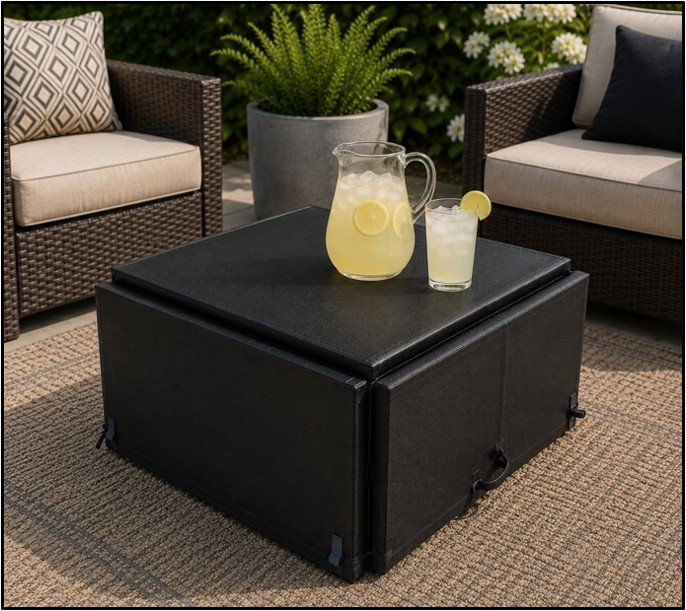
\includegraphics[
        width=1.92in,
        height=1.30in,
        keepaspectratio
    ]{generative_AI_concept_toro_cover_art}
};
\draw[RuleGray,line width=0.55pt,rounded corners=4pt]
    ($(current page.north west)+(7.00in,-5.04in)$)
    rectangle
    ($(current page.north west)+(9.08in,-6.43in)$);

% Image 5: folded foam functional prototype
% The portrait photograph is deliberately clipped to the landscape frame
% so the ottoman fills the card without extending beyond its border.
\begin{scope}
\clip[rounded corners=4pt]
    ($(current page.north west)+(9.19in,-5.04in)$)
    rectangle
    ($(current page.north east)+(-0.43in,-6.43in)$);

% Keep the original image proportions and center it within the existing card.
\node[anchor=center,inner sep=0pt]
at ($(current page.north west)+(9.88in,-5.735in)$)
{
    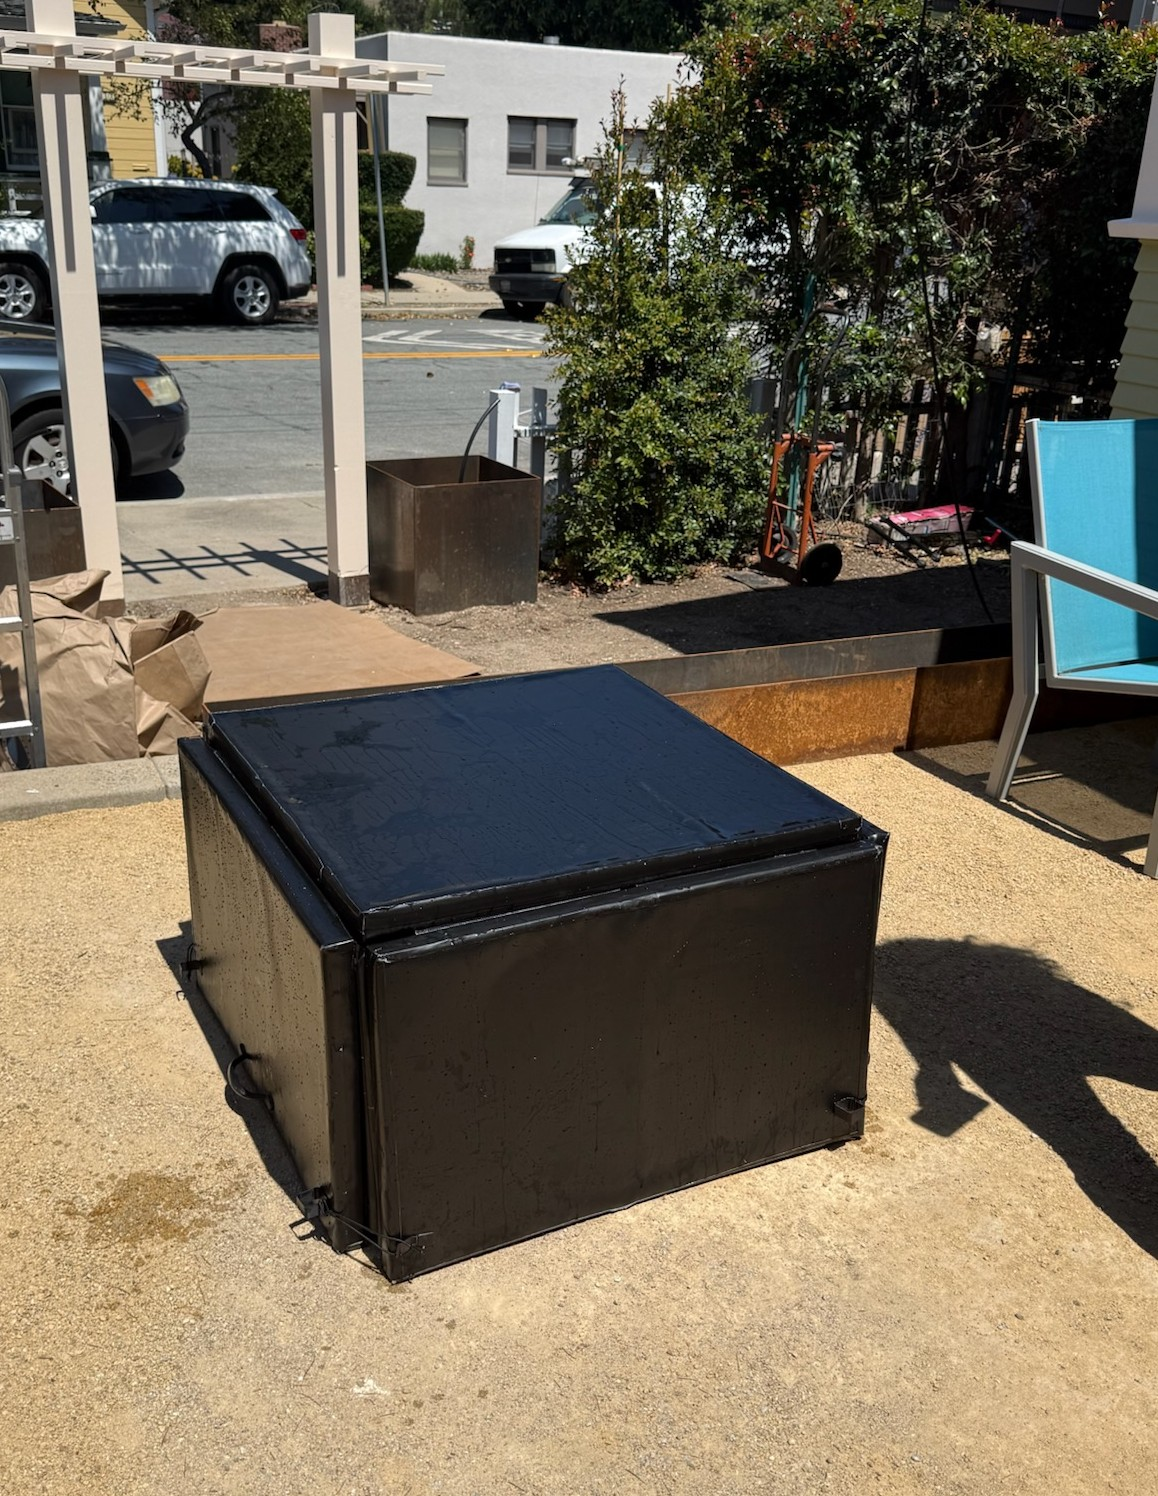
\includegraphics[
        width=1.58in,
        height=1.28in,
        keepaspectratio
    ]{foam_model_folded_backyard_image}
};
\end{scope}

\draw[RuleGray,line width=0.55pt,rounded corners=4pt]
    ($(current page.north west)+(9.19in,-5.04in)$)
    rectangle
    ($(current page.north east)+(-0.43in,-6.43in)$);

% Larger captions
\node[anchor=north,align=center,text width=1.95in,text=Muted,
      font=\sffamily\fontsize{6.8}{7.4}\selectfont]
at ($(current page.north west)+(1.47in,-6.49in)$)
{Topside panel architecture};

\node[anchor=north,align=center,text width=1.95in,text=Muted,
      font=\sffamily\fontsize{6.8}{7.4}\selectfont]
at ($(current page.north west)+(3.66in,-6.49in)$)
{Underside hinge architecture};

\node[anchor=north,align=center,text width=1.95in,text=Muted,
      font=\sffamily\fontsize{6.8}{7.4}\selectfont]
at ($(current page.north west)+(5.85in,-6.49in)$)
{Folded CAD configuration};

\node[anchor=north,align=center,text width=1.95in,text=Muted,
      font=\sffamily\fontsize{6.8}{7.4}\selectfont]
at ($(current page.north west)+(8.04in,-6.49in)$)
{Dual-use product vision};

\node[anchor=north,align=center,text width=1.95in,text=Muted,
      font=\sffamily\fontsize{6.8}{7.4}\selectfont]
at ($(current page.north west)+(9.88in,-6.49in)$)
{Folded foam prototype};

% Page 1 resource bar — centered and non-repeated resources
\fill[Panel,rounded corners=4pt]
    ($(current page.north west)+(0.43in,-7.05in)$)
    rectangle
    ($(current page.north east)+(-0.43in,-7.64in)$);
\draw[RuleGray,line width=0.5pt,rounded corners=4pt]
    ($(current page.north west)+(0.43in,-7.05in)$)
    rectangle
    ($(current page.north east)+(-0.43in,-7.64in)$);

\node[
    anchor=center,
    align=center,
    text=DeepGreen,
    font=\sffamily\bfseries\fontsize{6.9}{7.5}\selectfont
]
at ($(current page.north)+(0,-7.345in)$)
{\href{\ToroDrawingLink}{\faDraftingCompass\ DRAWING PACKAGE}
\hspace{24pt}
\href{\ToroDimensionsLink}{\faImage\ DIMENSION STUDY}
\hspace{24pt}
\href{\ToroProblemLink}{\faFileImage\ PROBLEM STATEMENT}};

% Footer
\node[
    anchor=south west,
    text=white,
    font=\sffamily\bfseries\fontsize{7.1}{7.7}\selectfont
]
at ($(current page.south west)+(0.42in,0.17in)$)
{\hyperlink{composites}{\faArrowLeft\ COMPOSITES}};

\node[
    anchor=south,
    text=white,
    font=\sffamily\fontsize{7.0}{7.6}\selectfont
]
at ($(current page.south)+(0,0.17in)$)
{TORO COVER \hspace{6pt} 1 / 3};

\node[
    anchor=south east,
    text=white,
    font=\sffamily\bfseries\fontsize{7.1}{7.7}\selectfont
]
at ($(current page.south east)+(-0.42in,0.17in)$)
{MANUFACTURING-DRIVEN DESIGN \faArrowRight};

\end{tikzpicture}


% ============================================================
% PAGE 2 — MANUFACTURING-DRIVEN DESIGN
% ============================================================

\clearpage
\thispagestyle{empty}
\hypertarget{toro-manufacturing}{}
\null

\begin{tikzpicture}[remember picture,overlay]

% Background and bars
\fill[white]
    (current page.south west)
    rectangle
    (current page.north east);

\fill[DeepGreen]
    (current page.north west)
    rectangle
    ($(current page.north east)+(0,-0.095in)$);

\fill[PolyGold]
    ($(current page.north west)+(0,-0.095in)$)
    rectangle
    ($(current page.north east)+(0,-0.14in)$);

\fill[DeepGreen]
    (current page.south west)
    rectangle
    ($(current page.south east)+(0,0.36in)$);

\fill[PolyGold]
    ($(current page.south west)+(0,0.36in)$)
    rectangle
    ($(current page.south east)+(0,0.405in)$);

% Header
\node[
    anchor=north west,
    text=PolyGold,
    font=\sffamily\bfseries\fontsize{8.1}{8.7}\selectfont
]
at ($(current page.north west)+(0.42in,-0.39in)$)
{TORO COVER \hspace{5pt}/\hspace{5pt} DESIGN FOR MANUFACTURABILITY};

\node[
    anchor=north west,
    text=DeepGreen,
    font=\bfseries\fontsize{23}{24}\selectfont
]
at ($(current page.north west)+(0.40in,-0.67in)$)
{THE ENVELOPE METHOD};

\node[
    anchor=north west,
    text=Muted,
    font=\sffamily\fontsize{8.7}{9.6}\selectfont
]
at ($(current page.north west)+(0.42in,-1.12in)$)
{A one-layup process developed for unusually thick insulated composite sandwich panels};

\fill[PolyGold]
    ($(current page.north west)+(0.42in,-1.36in)$)
    rectangle
    ($(current page.north west)+(5.30in,-1.315in)$);

% Process explanation
\fill[SoftGold,rounded corners=5pt]
    ($(current page.north west)+(0.42in,-1.61in)$)
    rectangle
    ($(current page.north east)+(-0.42in,-2.90in)$);

\fill[PolyGold]
    ($(current page.north west)+(0.42in,-1.61in)$)
    rectangle
    ($(current page.north west)+(0.52in,-2.90in)$);

\node[
    anchor=north west,
    text=DeepGreen,
    font=\sffamily\bfseries\fontsize{7.9}{8.6}\selectfont
]
at ($(current page.north west)+(0.67in,-1.76in)$)
{PROCESS INNOVATION};

\node[
    anchor=north west,
    align=left,
    text width=9.55in,
    text=Ink,
    font=\fontsize{7.35}{8.75}\selectfont
]
at ($(current page.north west)+(0.67in,-2.02in)$)
{
Weight reduction and insulation were both essential, leading to the selection of an
XPS foam core. Because XPS could not tolerate composite heat-cure temperatures, prepreg
processing was not practical and the panels had to be manufactured by wet layup with a
room-temperature cure. To simplify this process, I waterjet-cut XPS perimeter strips from
excess foam and placed them around each core inside the vacuum enclosure. Under vacuum,
the top and bottom carbon skins met along the panel sides and compressed against this
border, eliminating a separate edge-banding layup and reducing corner pleating.
};

% Workflow title
\node[
    anchor=north west,
    text=DeepGreen,
    font=\sffamily\bfseries\fontsize{8.0}{8.7}\selectfont
]
at ($(current page.north west)+(0.43in,-3.06in)$)
{MANUFACTURING WORKFLOW};

% Row 1 image 1
\node[anchor=center,inner sep=0pt]
at ($(current page.north west)+(2.07in,-4.105in)$)
{
    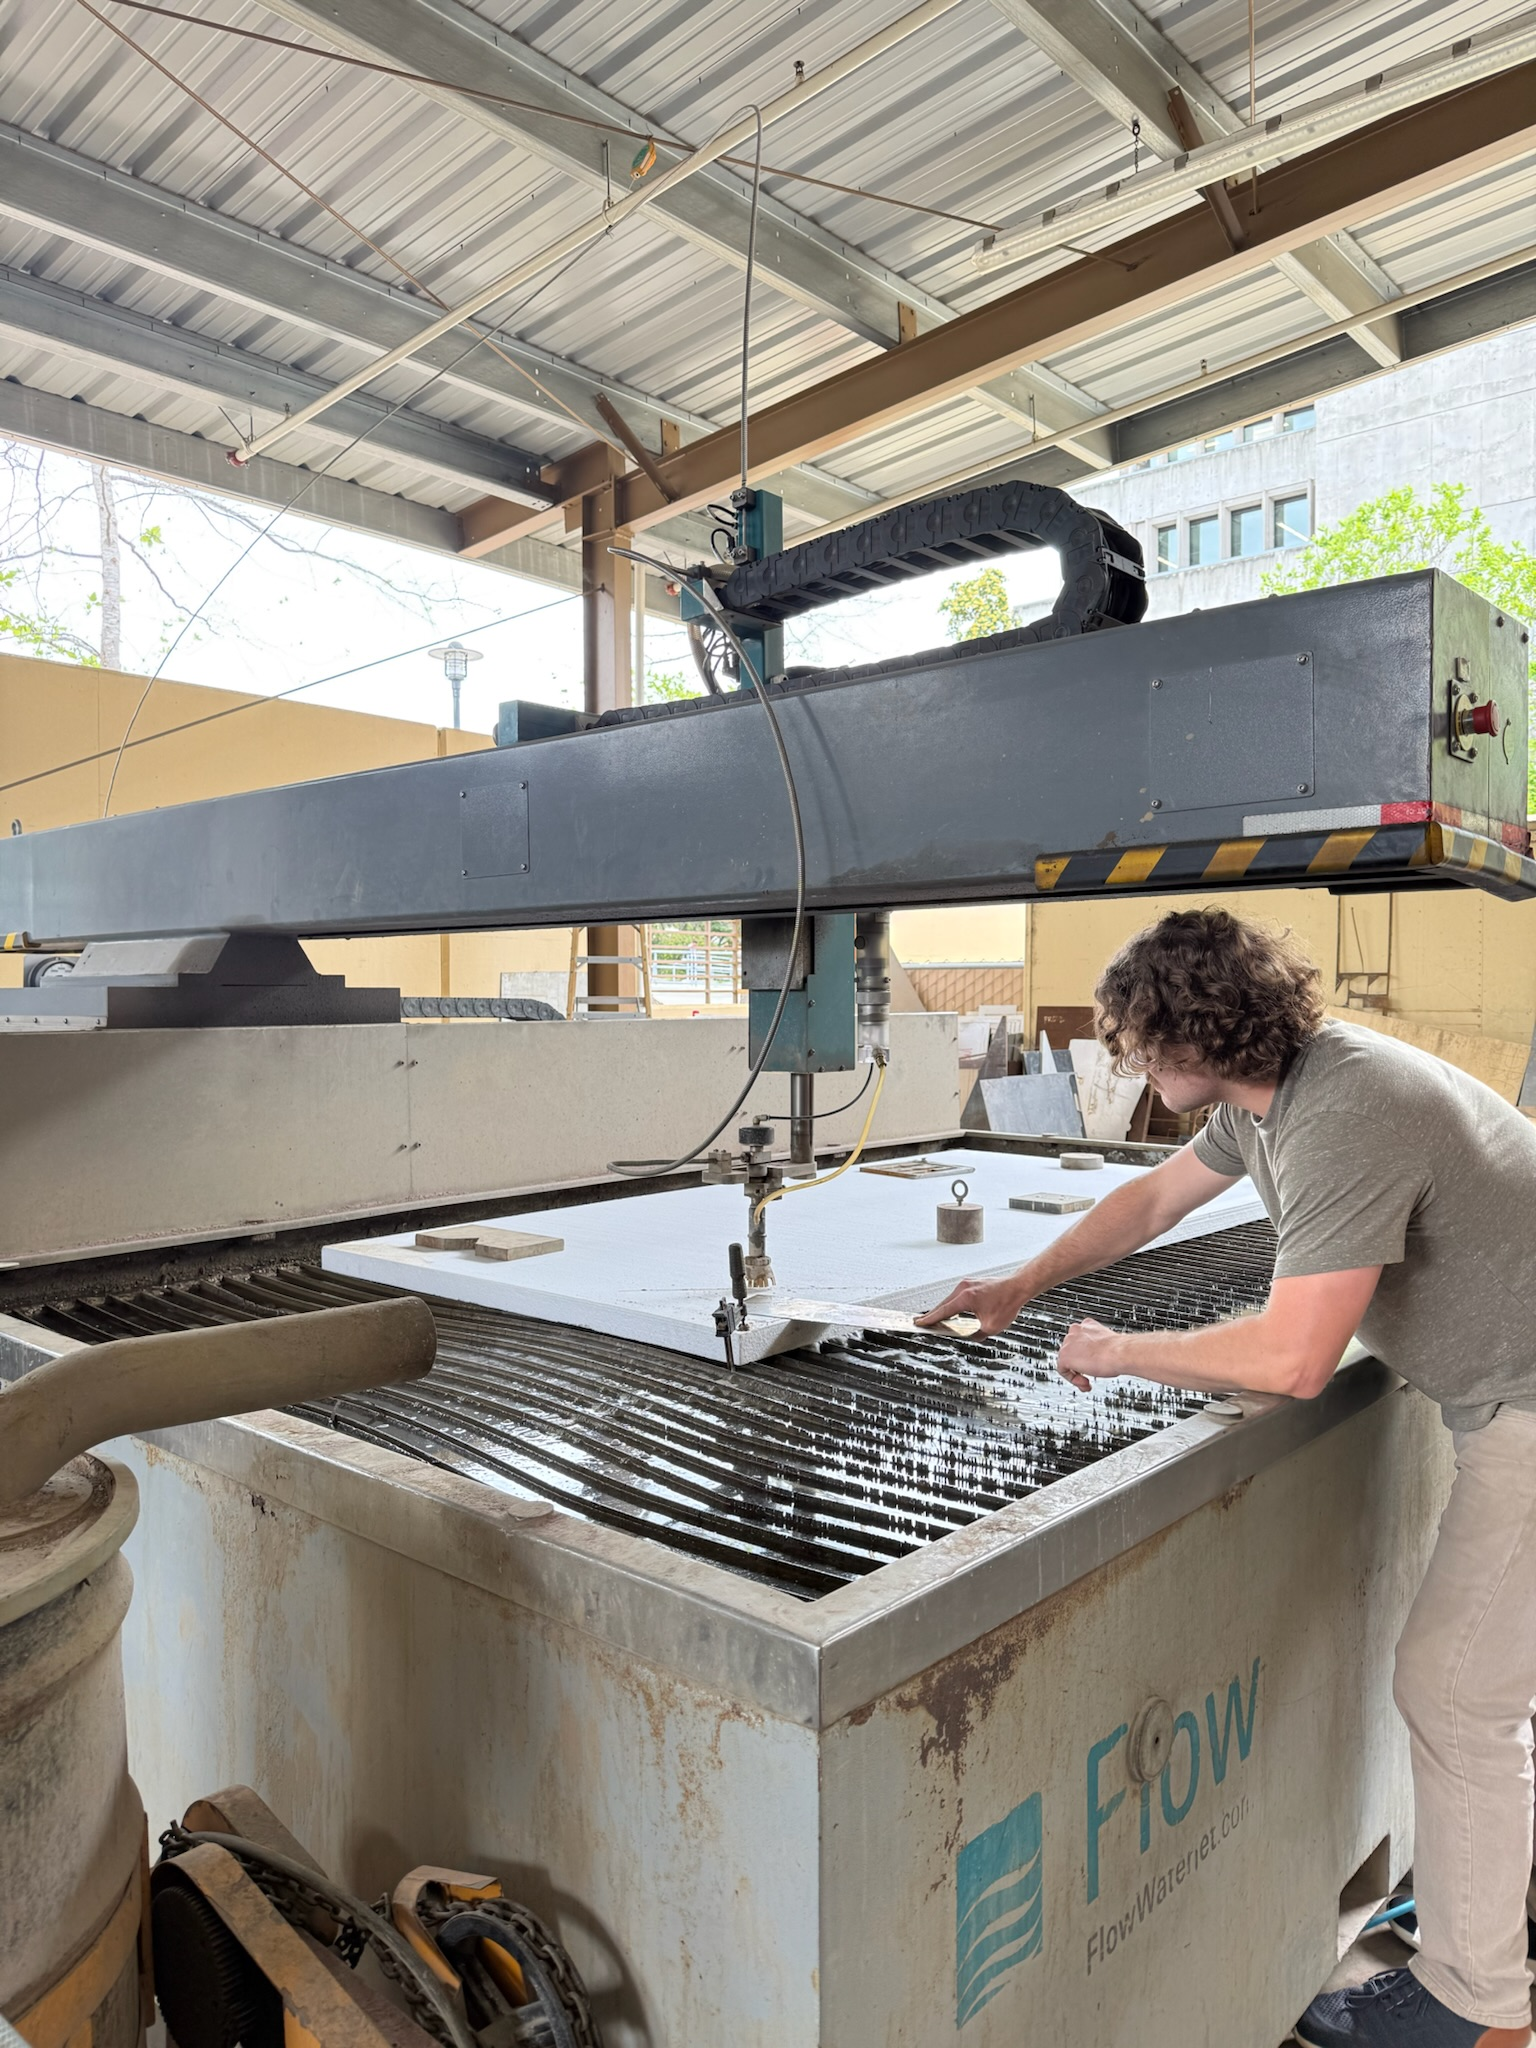
\includegraphics[
        width=3.10in,
        height=1.40in,
        keepaspectratio
    ]{waterjet_foam}
};
\draw[RuleGray,line width=0.55pt,rounded corners=4pt]
    ($(current page.north west)+(0.43in,-3.36in)$)
    rectangle
    ($(current page.north west)+(3.71in,-4.85in)$);

% Row 1 image 2
\node[anchor=center,inner sep=0pt]
at ($(current page.north west)+(5.50in,-4.105in)$)
{
    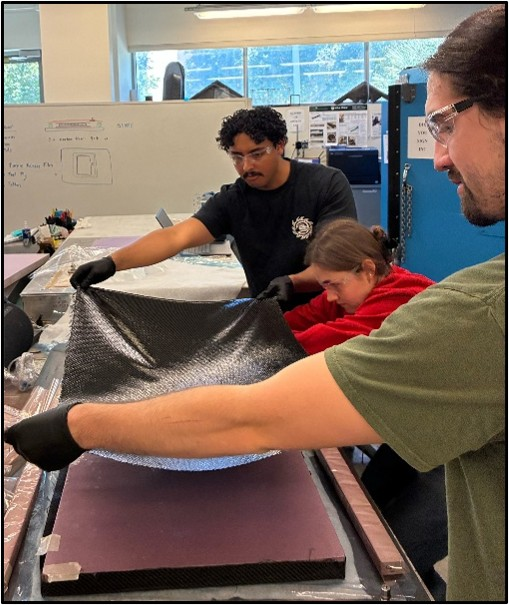
\includegraphics[
        width=3.10in,
        height=1.40in,
        keepaspectratio
    ]{group_layup}
};
\draw[RuleGray,line width=0.55pt,rounded corners=4pt]
    ($(current page.north west)+(3.86in,-3.36in)$)
    rectangle
    ($(current page.north west)+(7.14in,-4.85in)$);

% Row 1 image 3
\node[anchor=center,inner sep=0pt]
at ($(current page.north west)+(8.935in,-4.105in)$)
{
    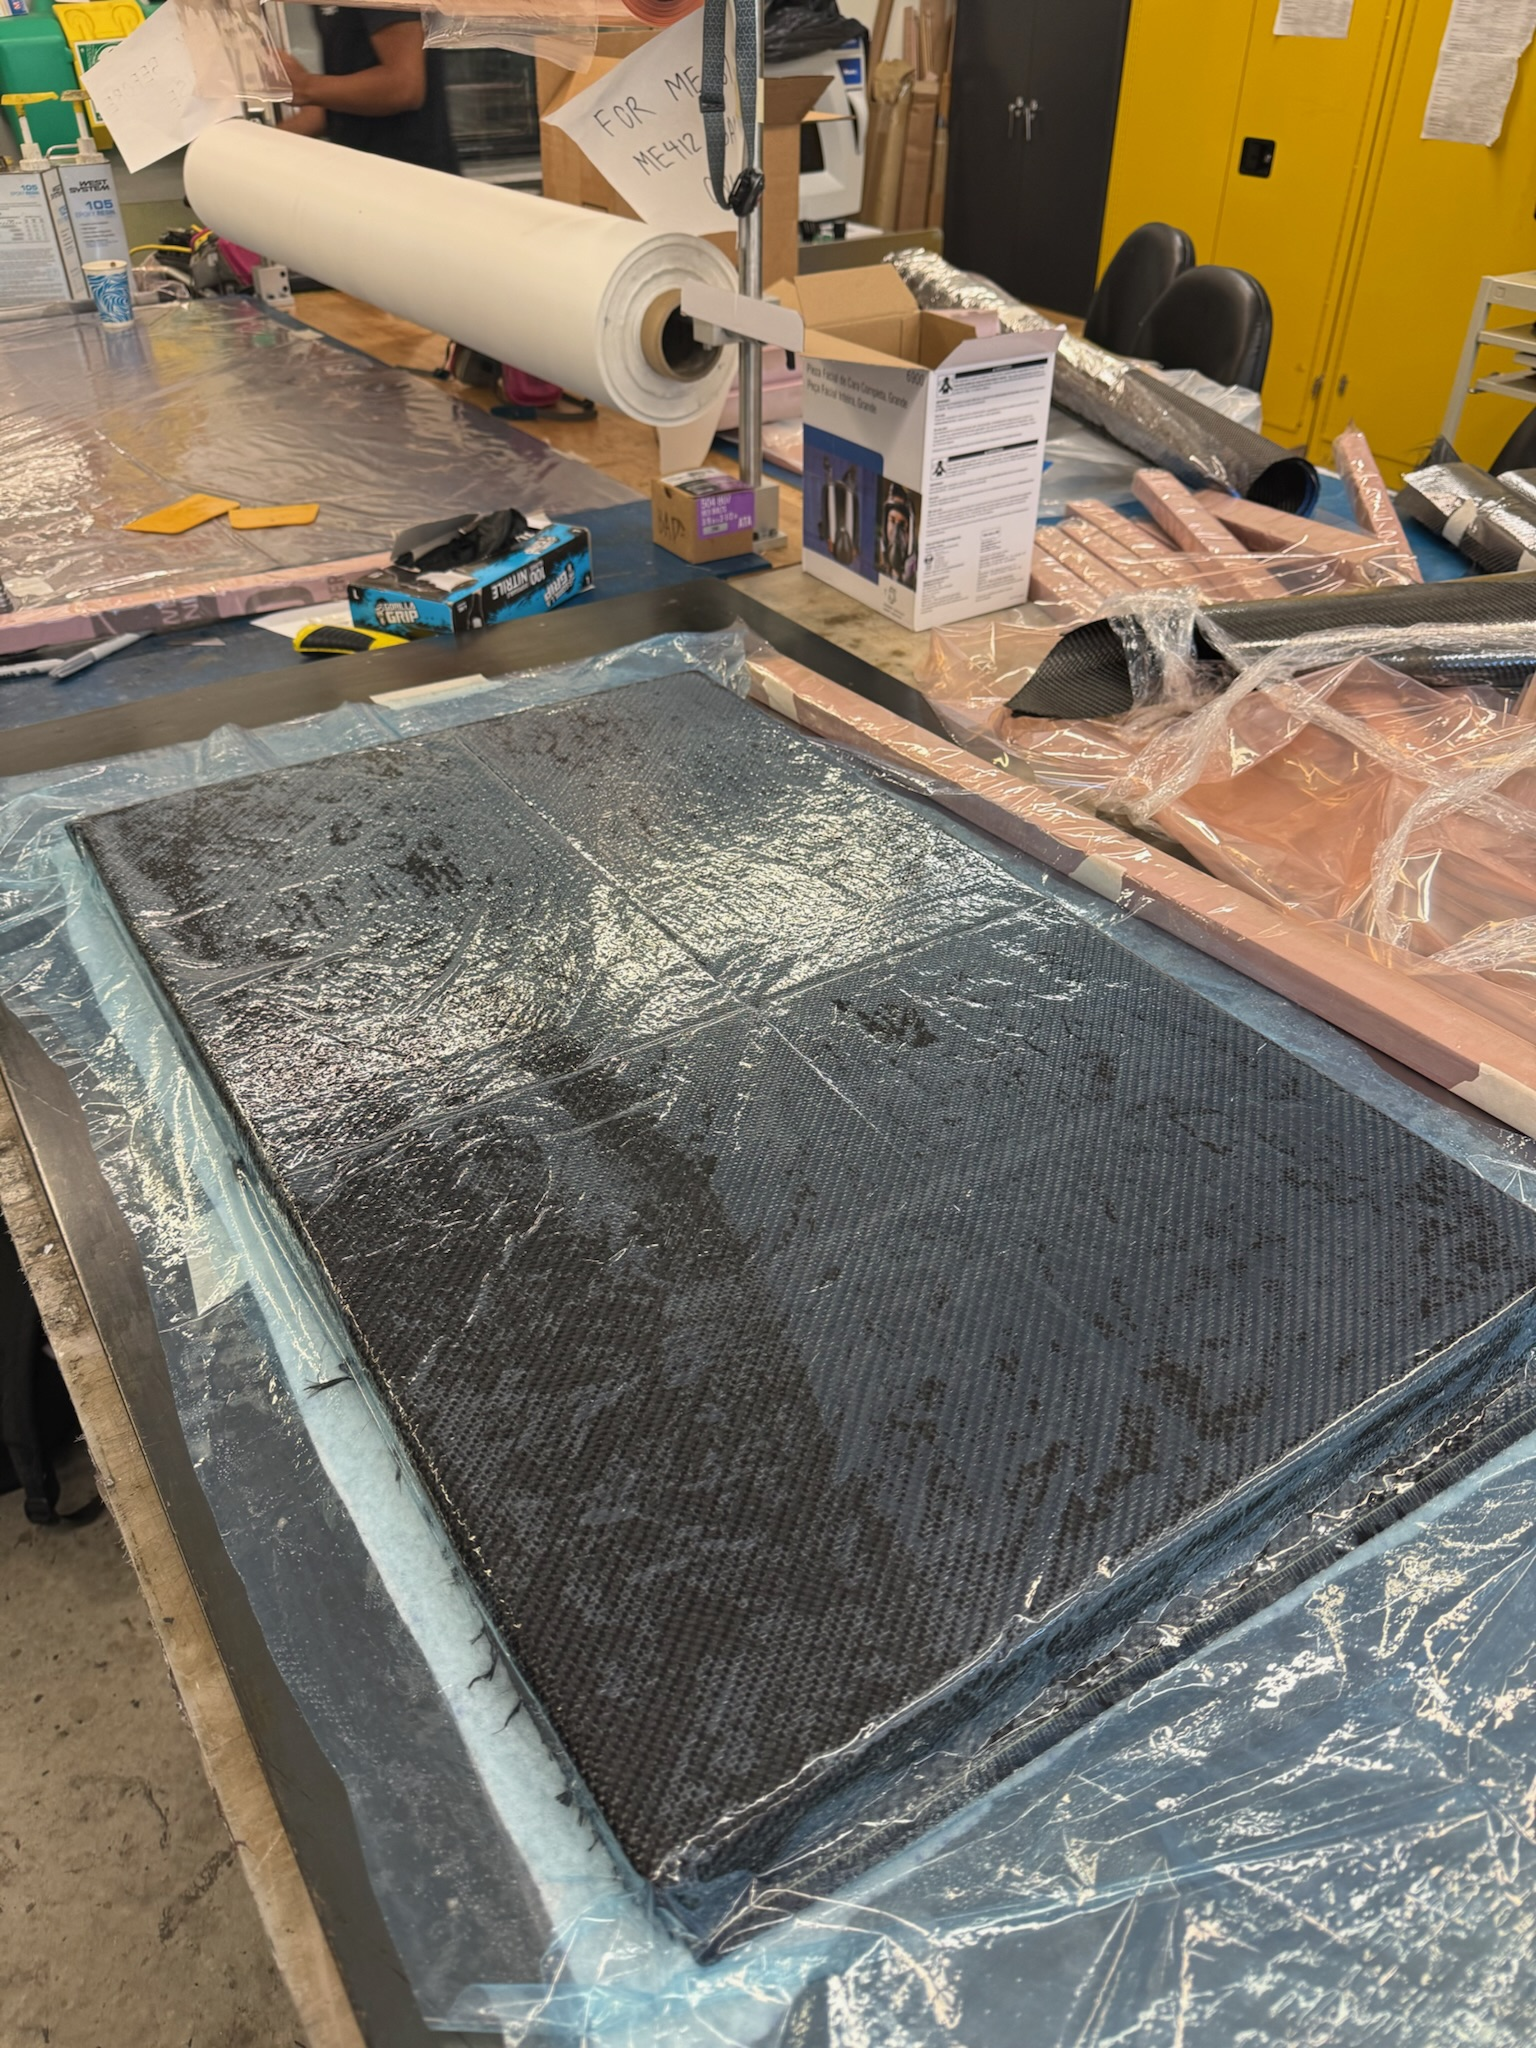
\includegraphics[
        width=3.10in,
        height=1.40in,
        keepaspectratio
    ]{blue_perforrated_film_layup}
};
\draw[RuleGray,line width=0.55pt,rounded corners=4pt]
    ($(current page.north west)+(7.29in,-3.36in)$)
    rectangle
    ($(current page.north east)+(-0.42in,-4.85in)$);

% Row 1 captions
\node[anchor=north,text=Muted,font=\sffamily\fontsize{6.7}{7.3}\selectfont]
at ($(current page.north west)+(2.07in,-4.90in)$)
{1. Waterjet-cut core and perimeter geometry};

\node[anchor=north,text=Muted,font=\sffamily\fontsize{6.7}{7.3}\selectfont]
at ($(current page.north west)+(5.50in,-4.90in)$)
{2. Team wet layup under my process guidance};

\node[anchor=north,text=Muted,font=\sffamily\fontsize{6.7}{7.3}\selectfont]
at ($(current page.north west)+(8.935in,-4.90in)$)
{3. Perforated film, breather, and vacuum enclosure};

% Row 2 image 1
\node[anchor=center,inner sep=0pt]
at ($(current page.north west)+(2.07in,-5.875in)$)
{
    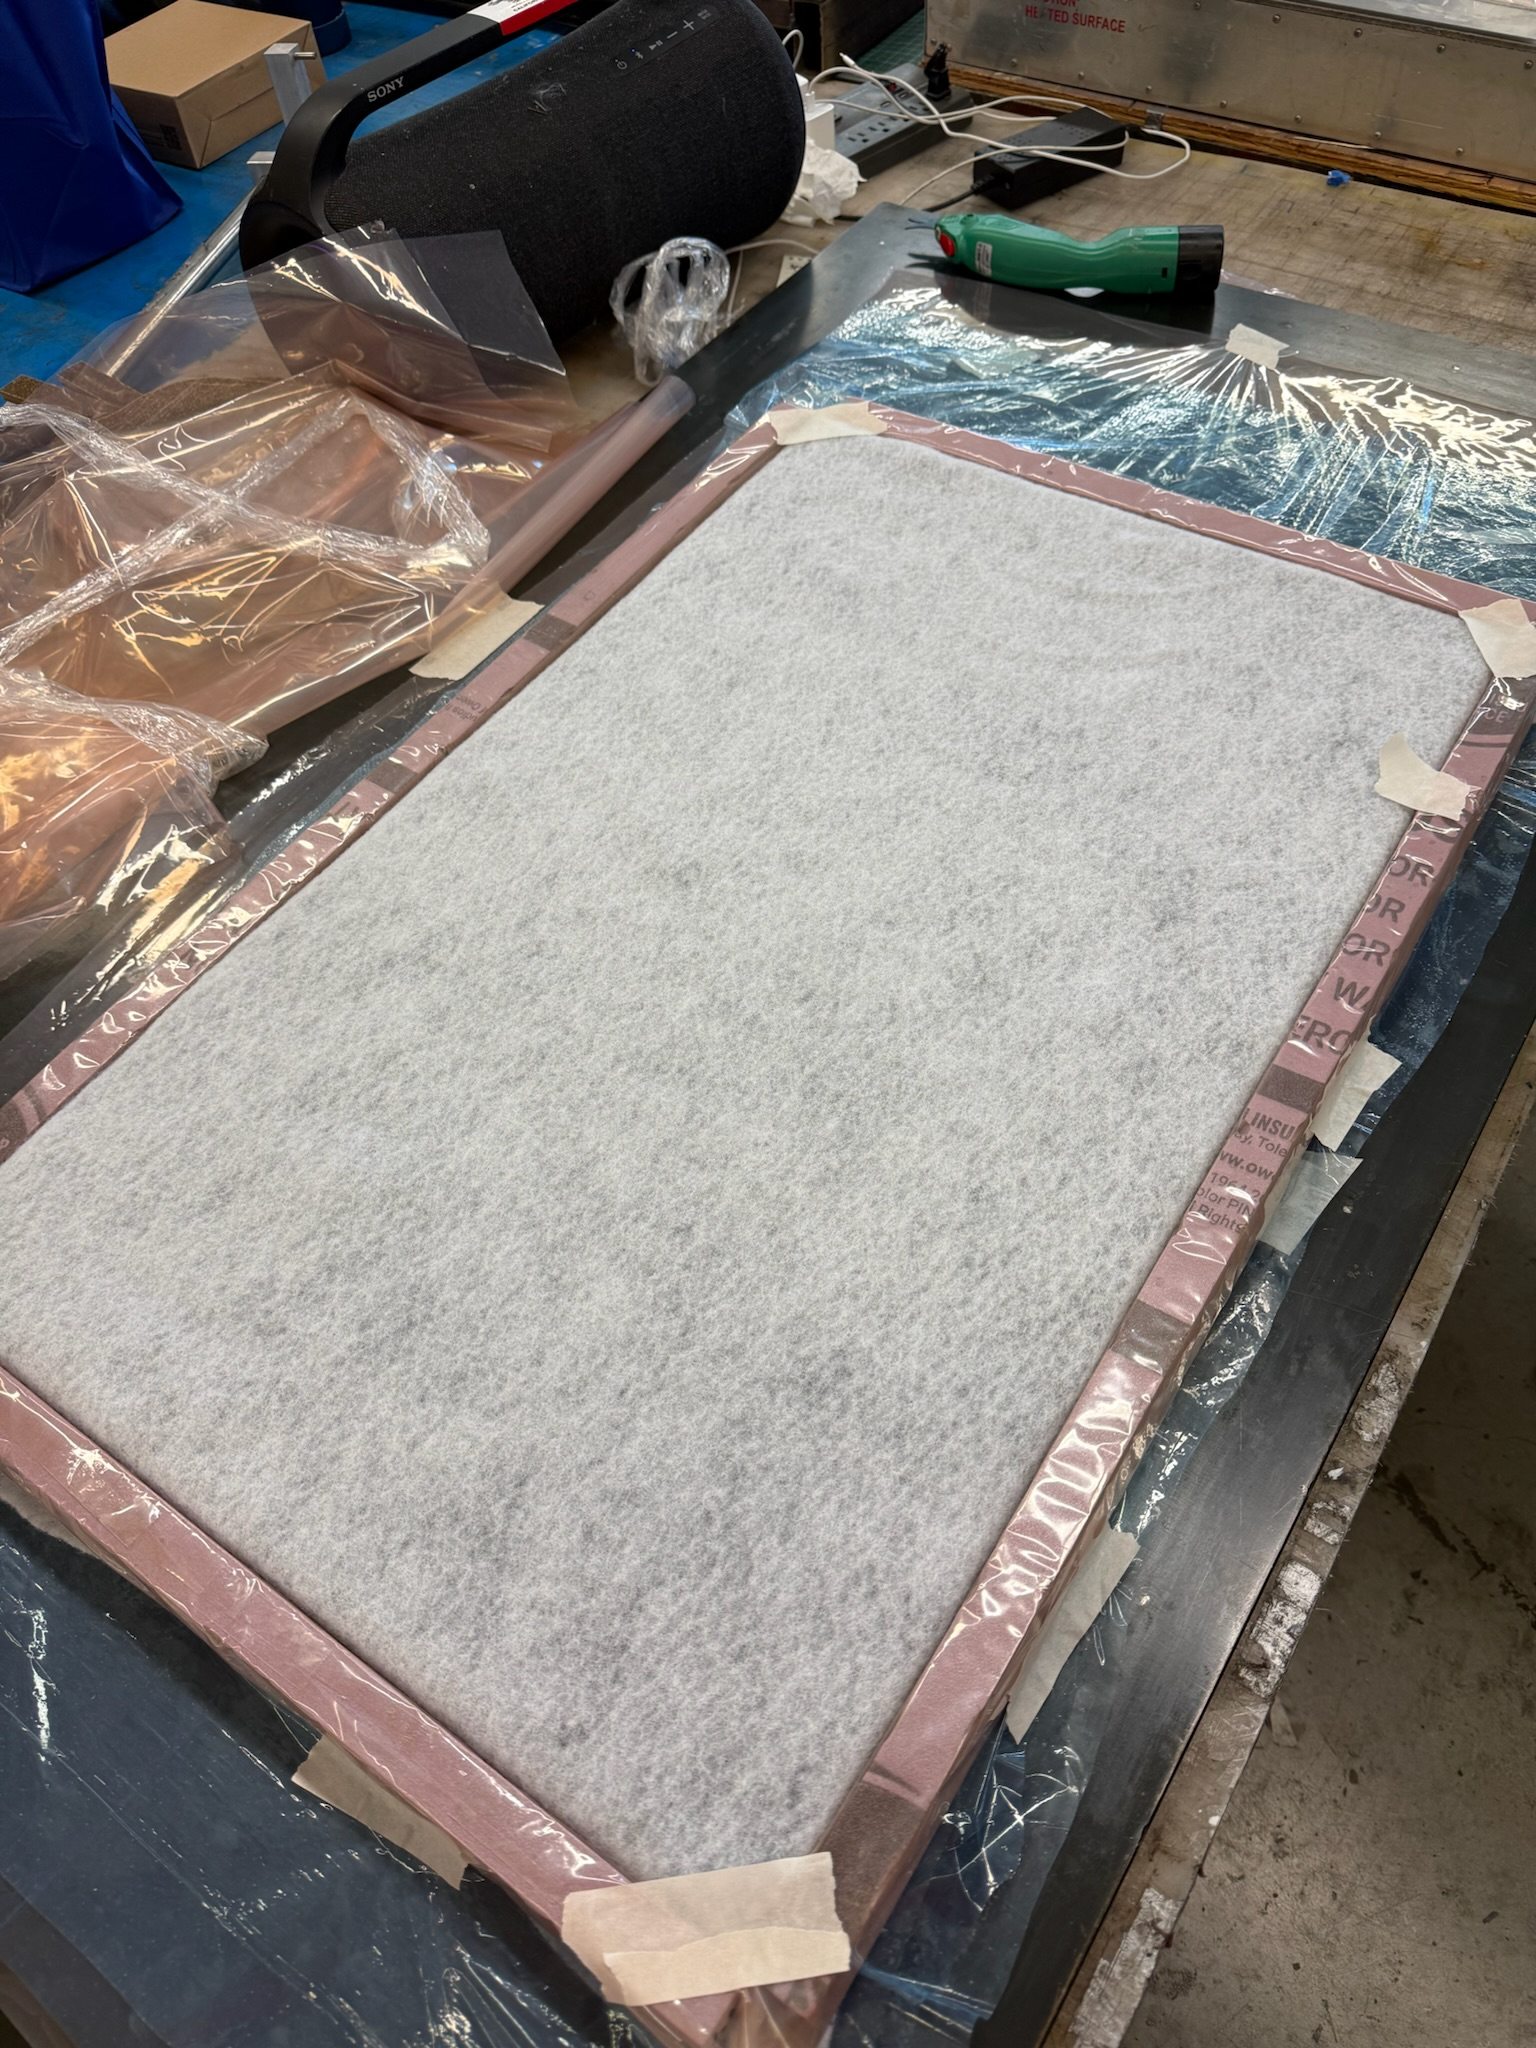
\includegraphics[
        width=3.10in,
        height=1.40in,
        keepaspectratio
    ]{completed_layup}
};
\draw[RuleGray,line width=0.55pt,rounded corners=4pt]
    ($(current page.north west)+(0.43in,-5.13in)$)
    rectangle
    ($(current page.north west)+(3.71in,-6.62in)$);

% Row 2 image 2 — oven chamber used only as a reliable vacuum enclosure; no heat applied
\node[anchor=center,inner sep=0pt]
at ($(current page.north west)+(5.50in,-5.875in)$)
{
    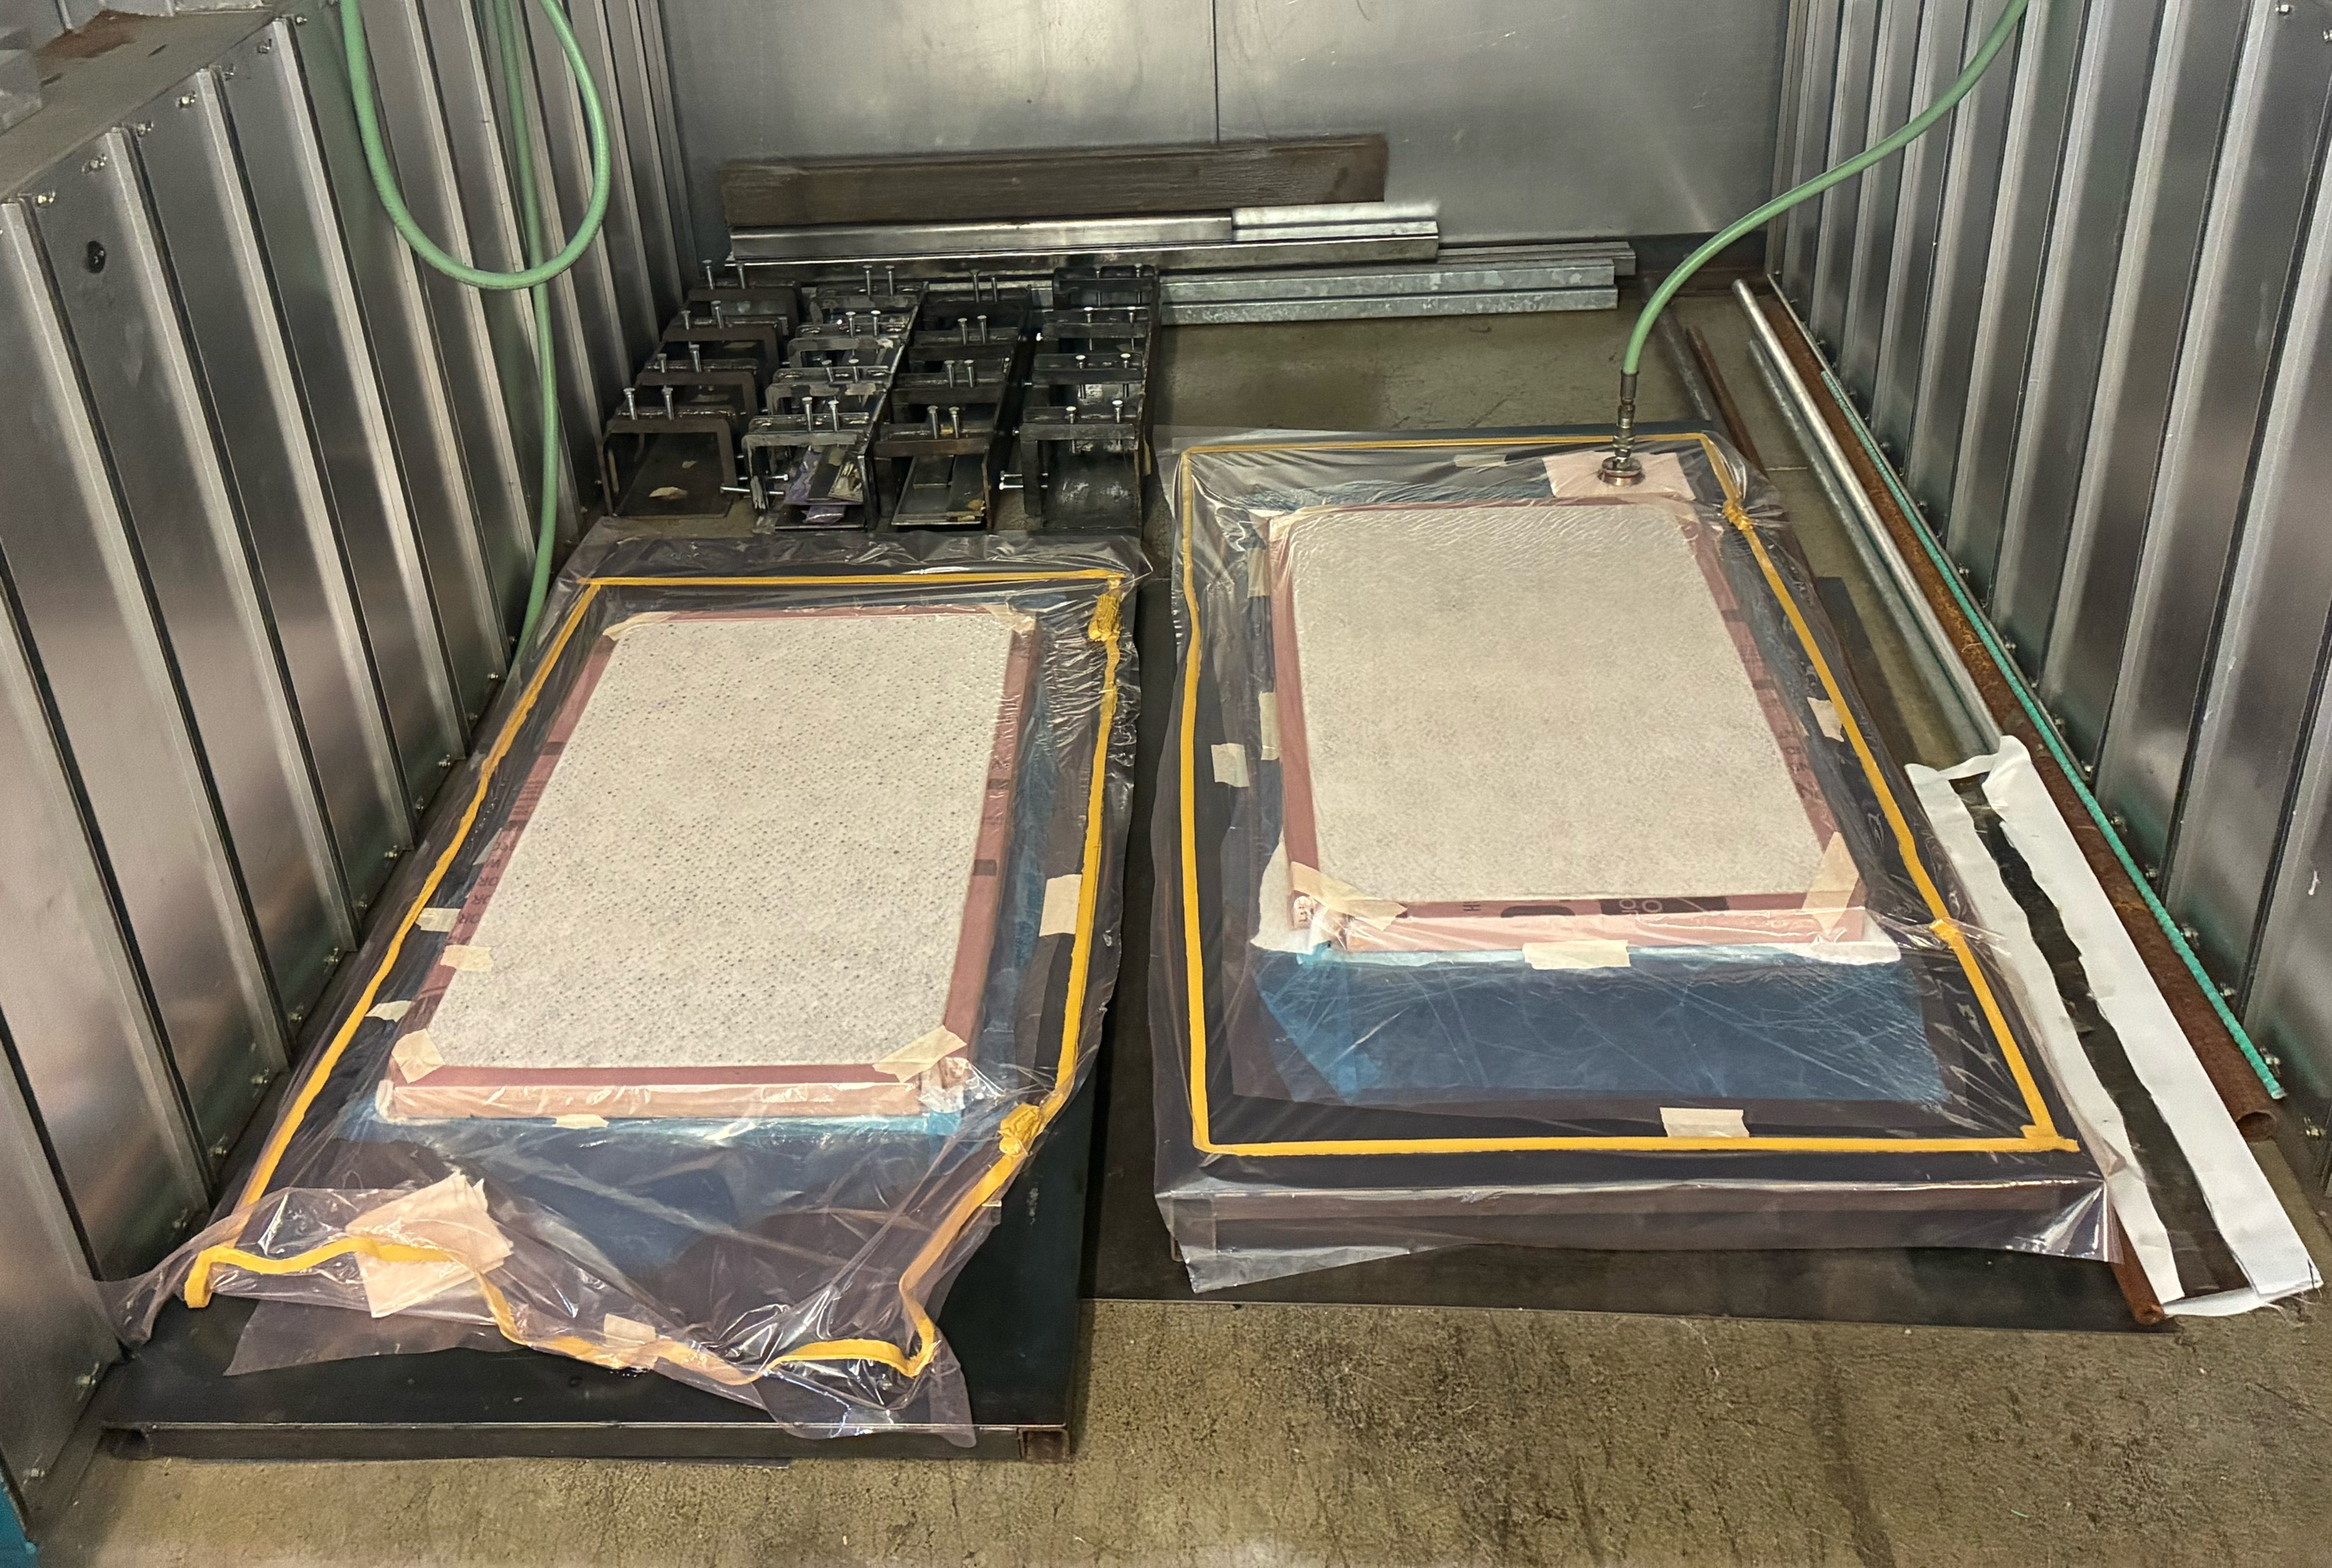
\includegraphics[
        width=3.10in,
        height=1.40in,
        keepaspectratio
    ]{layups_in_composite_oven_under_vacuumPressure}
};
\draw[RuleGray,line width=0.55pt,rounded corners=4pt]
    ($(current page.north west)+(3.86in,-5.13in)$)
    rectangle
    ($(current page.north west)+(7.14in,-6.62in)$);

% Row 2 image 3
\node[anchor=center,inner sep=0pt]
at ($(current page.north west)+(8.935in,-5.875in)$)
{
    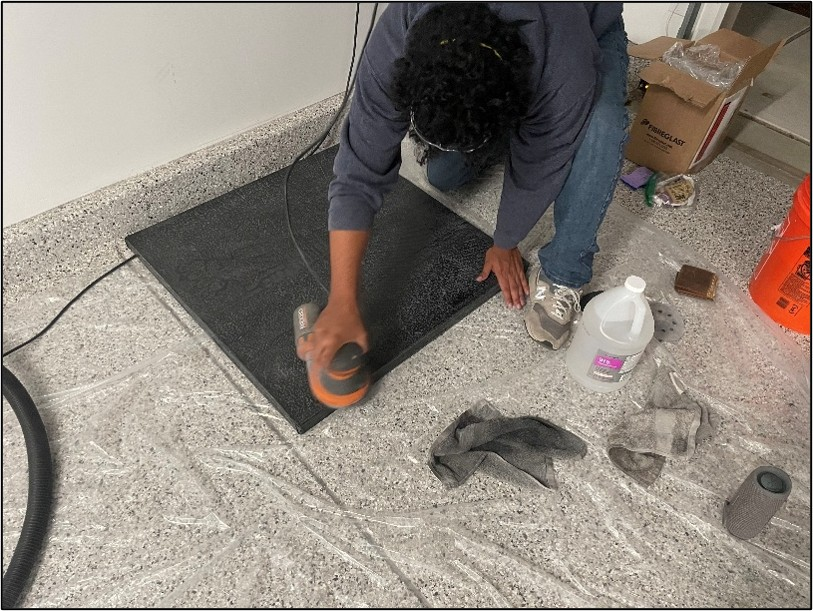
\includegraphics[
        width=3.10in,
        height=1.40in,
        keepaspectratio
    ]{garage_sanding}
};
\draw[RuleGray,line width=0.55pt,rounded corners=4pt]
    ($(current page.north west)+(7.29in,-5.13in)$)
    rectangle
    ($(current page.north east)+(-0.42in,-6.62in)$);

% Row 2 captions
\node[anchor=north,text=Muted,font=\sffamily\fontsize{6.7}{7.3}\selectfont]
at ($(current page.north west)+(2.07in,-6.67in)$)
{4. Fully saturated carbon skin and foam sandwich};

\node[anchor=north,text=Muted,font=\sffamily\fontsize{6.7}{7.3}\selectfont]
at ($(current page.north west)+(5.50in,-6.67in)$)
{5. Room-temperature cure under continuous vacuum};

\node[anchor=north,text=Muted,font=\sffamily\fontsize{6.7}{7.3}\selectfont]
at ($(current page.north west)+(8.935in,-6.67in)$)
{6. Post-processing and surface preparation};

% Bottom callouts
\fill[Panel,rounded corners=4pt]
    ($(current page.north west)+(0.43in,-6.95in)$)
    rectangle
    ($(current page.north west)+(5.48in,-7.60in)$);

\draw[RuleGray,line width=0.55pt,rounded corners=4pt]
    ($(current page.north west)+(0.43in,-6.95in)$)
    rectangle
    ($(current page.north west)+(5.48in,-7.60in)$);

\node[
    anchor=north west,
    text=DeepGreen,
    font=\sffamily\bfseries\fontsize{7.0}{7.6}\selectfont
]
at ($(current page.north west)+(0.63in,-7.08in)$)
{FROM THREE LAYUPS TO ONE};

\node[
    anchor=north west,
    align=left,
    text width=4.56in,
    text=Ink,
    font=\fontsize{6.45}{7.45}\selectfont
]
at ($(current page.north west)+(0.63in,-7.29in)$)
{
The Envelope Method reduced labor, cure cycles, handling,
alignment risk, and time spent forming numerous vacuum-bag
pleats around the 1.5-inch-thick XPS panels.
};

\fill[Panel,rounded corners=4pt]
    ($(current page.north west)+(5.68in,-6.95in)$)
    rectangle
    ($(current page.north east)+(-0.42in,-7.60in)$);

\draw[RuleGray,line width=0.55pt,rounded corners=4pt]
    ($(current page.north west)+(5.68in,-6.95in)$)
    rectangle
    ($(current page.north east)+(-0.42in,-7.60in)$);

\node[
    anchor=north west,
    text=DeepGreen,
    font=\sffamily\bfseries\fontsize{7.0}{7.6}\selectfont
]
at ($(current page.north west)+(5.88in,-7.08in)$)
{WHY SURFACE-BONDED HARDWARE};

\node[
    anchor=north west,
    align=left,
    text width=4.55in,
    text=Ink,
    font=\fontsize{6.45}{7.45}\selectfont
]
at ($(current page.north west)+(5.88in,-7.29in)$)
{
Adhesively bonded hinges and fixtures preserved the clean
composite exterior and avoided drilled inserts, foam-core
crushing, added stress concentrations, and new leak paths.
};


% Footer
\node[
    anchor=south west,
    text=white,
    font=\sffamily\bfseries\fontsize{7.1}{7.7}\selectfont
]
at ($(current page.south west)+(0.42in,0.17in)$)
{\faArrowLeft\ PRODUCT ARCHITECTURE};

\node[
    anchor=south,
    text=white,
    font=\sffamily\fontsize{7.0}{7.6}\selectfont
]
at ($(current page.south)+(0,0.17in)$)
{TORO COVER \hspace{6pt} 2 / 3};

\node[
    anchor=south east,
    text=white,
    font=\sffamily\bfseries\fontsize{7.1}{7.7}\selectfont
]
at ($(current page.south east)+(-0.42in,0.17in)$)
{VALIDATION \& TAKEAWAYS \faArrowRight};

\end{tikzpicture}


% ============================================================
% PAGE 3 — FINISHING, VALIDATION, AND TAKEAWAYS
% ============================================================

\clearpage
\thispagestyle{empty}
\hypertarget{toro-results}{}
\null

\begin{tikzpicture}[remember picture,overlay]

% Background and bars
\fill[white]
    (current page.south west)
    rectangle
    (current page.north east);

\fill[DeepGreen]
    (current page.north west)
    rectangle
    ($(current page.north east)+(0,-0.095in)$);

\fill[PolyGold]
    ($(current page.north west)+(0,-0.095in)$)
    rectangle
    ($(current page.north east)+(0,-0.14in)$);

\fill[DeepGreen]
    (current page.south west)
    rectangle
    ($(current page.south east)+(0,0.36in)$);

\fill[PolyGold]
    ($(current page.south west)+(0,0.36in)$)
    rectangle
    ($(current page.south east)+(0,0.405in)$);

% Header
\node[
    anchor=north west,
    text=PolyGold,
    font=\sffamily\bfseries\fontsize{8.1}{8.7}\selectfont
]
at ($(current page.north west)+(0.42in,-0.39in)$)
{TORO COVER \hspace{5pt}/\hspace{5pt} VALIDATION AND ENGINEERING TAKEAWAYS};

\node[
    anchor=north west,
    text=DeepGreen,
    font=\bfseries\fontsize{22.5}{23.5}\selectfont
]
at ($(current page.north west)+(0.40in,-0.67in)$)
{FROM PROTOTYPE TO PRODUCT PATHWAY};

\node[
    anchor=north west,
    text=Muted,
    font=\sffamily\fontsize{8.7}{9.6}\selectfont
]
at ($(current page.north west)+(0.42in,-1.12in)$)
{Environmental protection, usability testing, scope decisions, and lessons from technical leadership};

\fill[PolyGold]
    ($(current page.north west)+(0.42in,-1.36in)$)
    rectangle
    ($(current page.north west)+(5.8in,-1.315in)$);

% Finishing title
\node[
    anchor=north west,
    text=DeepGreen,
    font=\sffamily\bfseries\fontsize{8.0}{8.7}\selectfont
]
at ($(current page.north west)+(0.43in,-1.62in)$)
{OUTDOOR FINISHING AND ENVIRONMENTAL PROTECTION};

% Image 1
\node[anchor=center,inner sep=0pt]
at ($(current page.north west)+(1.705in,-2.655in)$)
{
    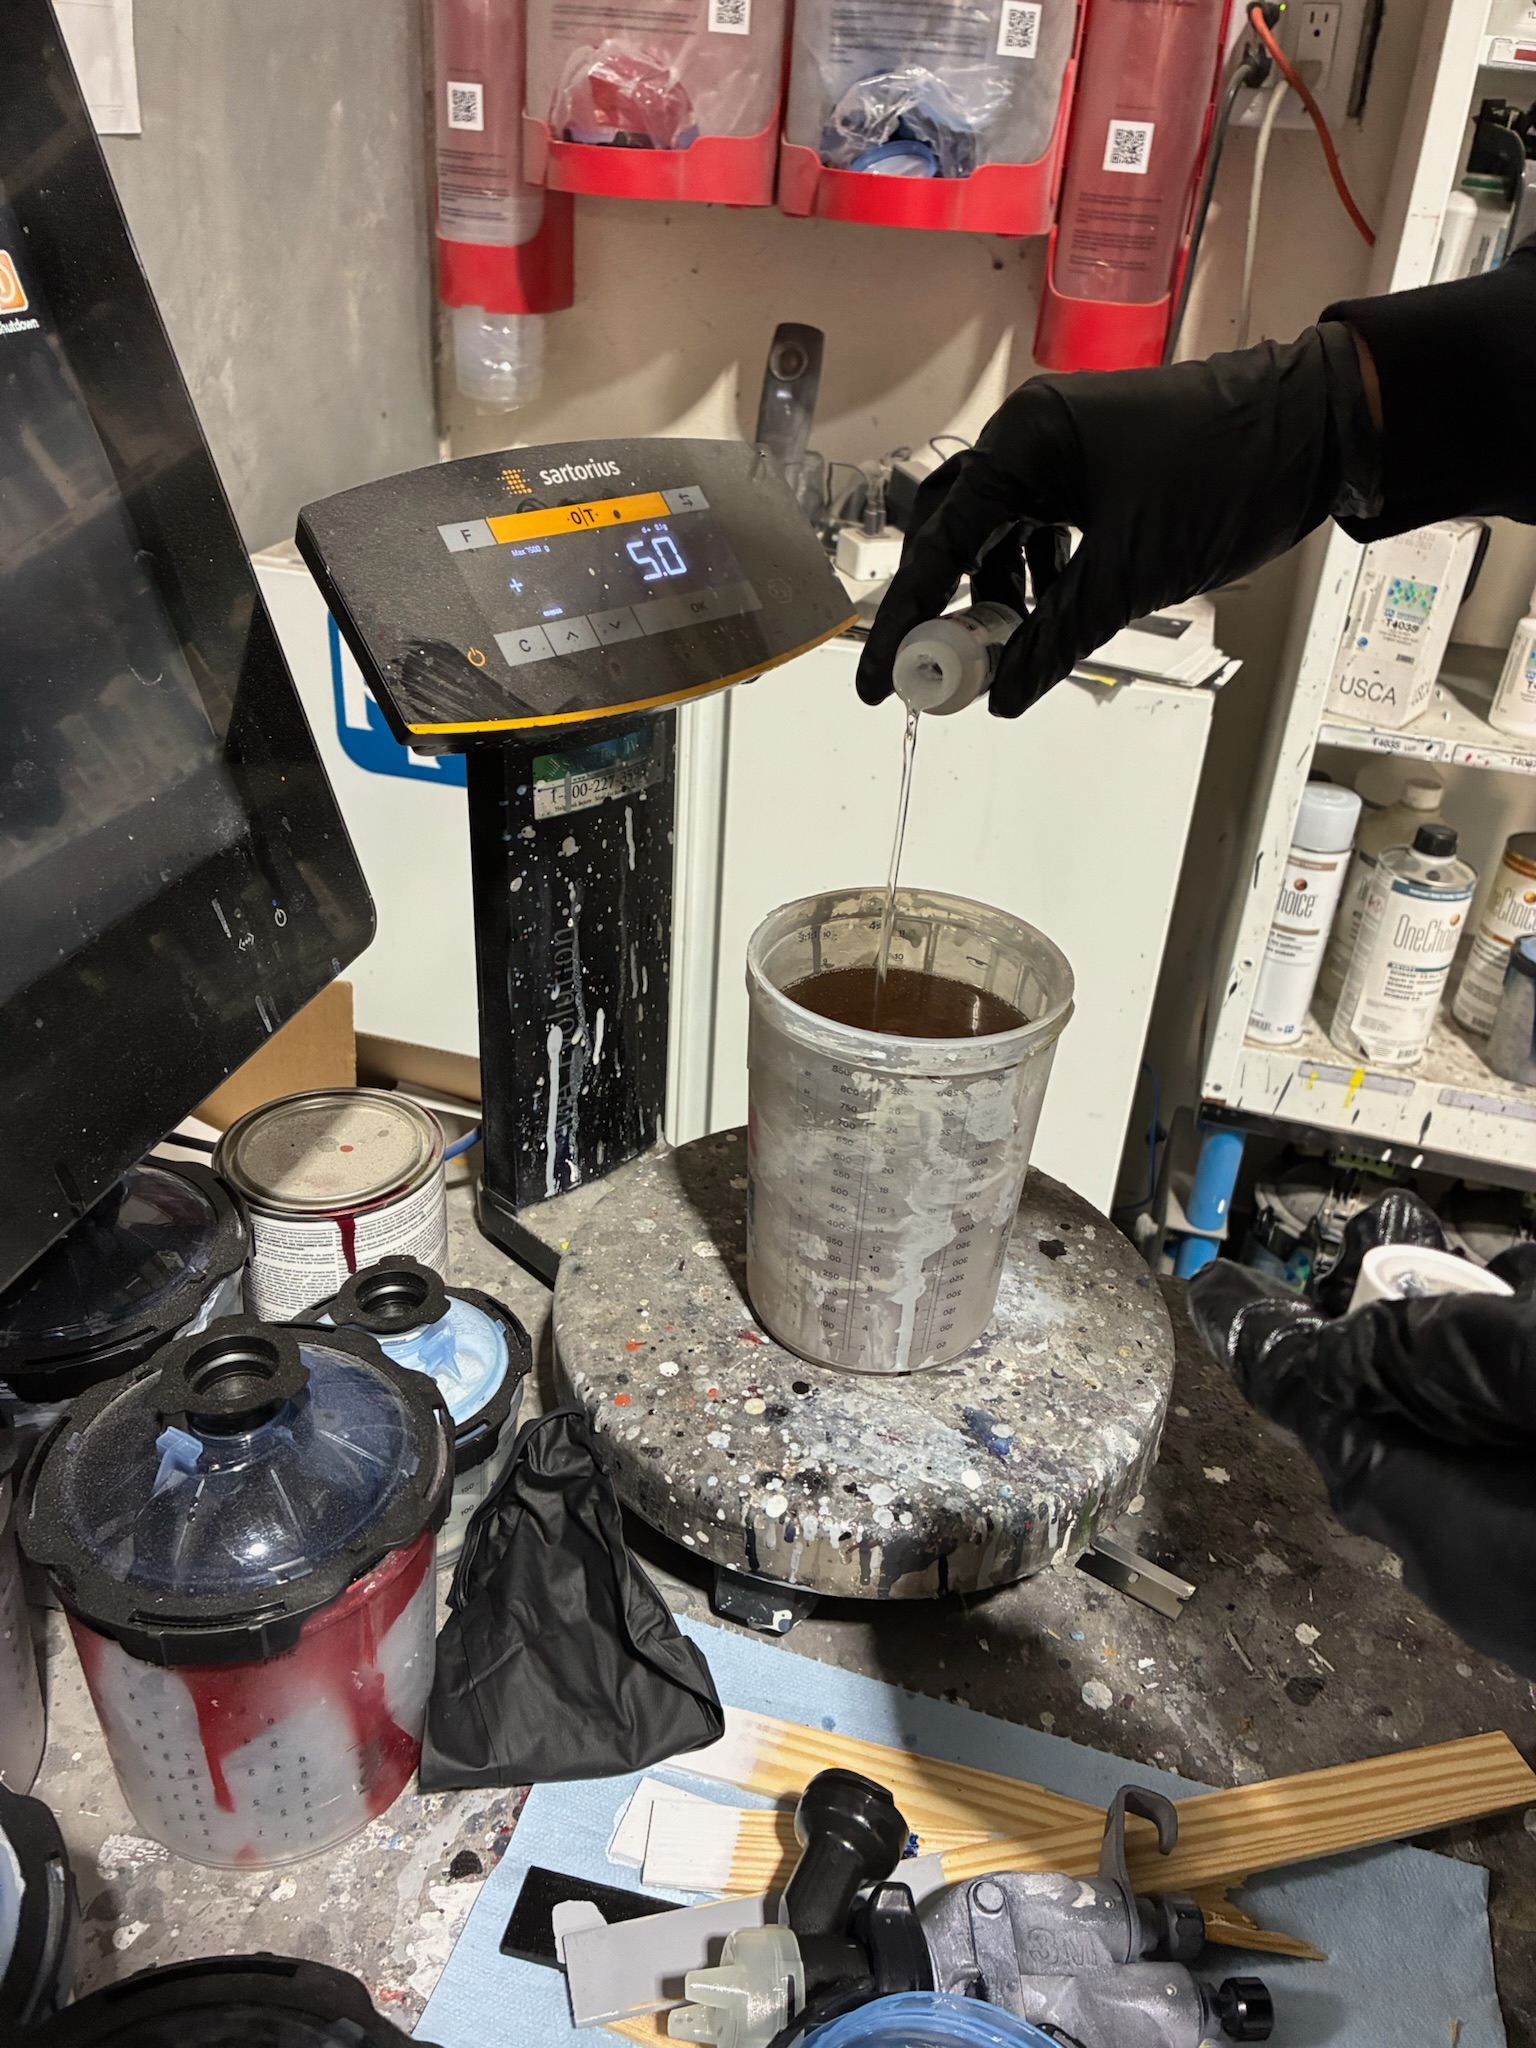
\includegraphics[
        width=2.35in,
        height=1.40in,
        keepaspectratio
    ]{spray_topcoat_prep}
};
\draw[RuleGray,line width=0.55pt,rounded corners=4pt]
    ($(current page.north west)+(0.43in,-1.91in)$)
    rectangle
    ($(current page.north west)+(2.98in,-3.40in)$);

% Image 2
\node[anchor=center,inner sep=0pt]
at ($(current page.north west)+(4.375in,-2.655in)$)
{
    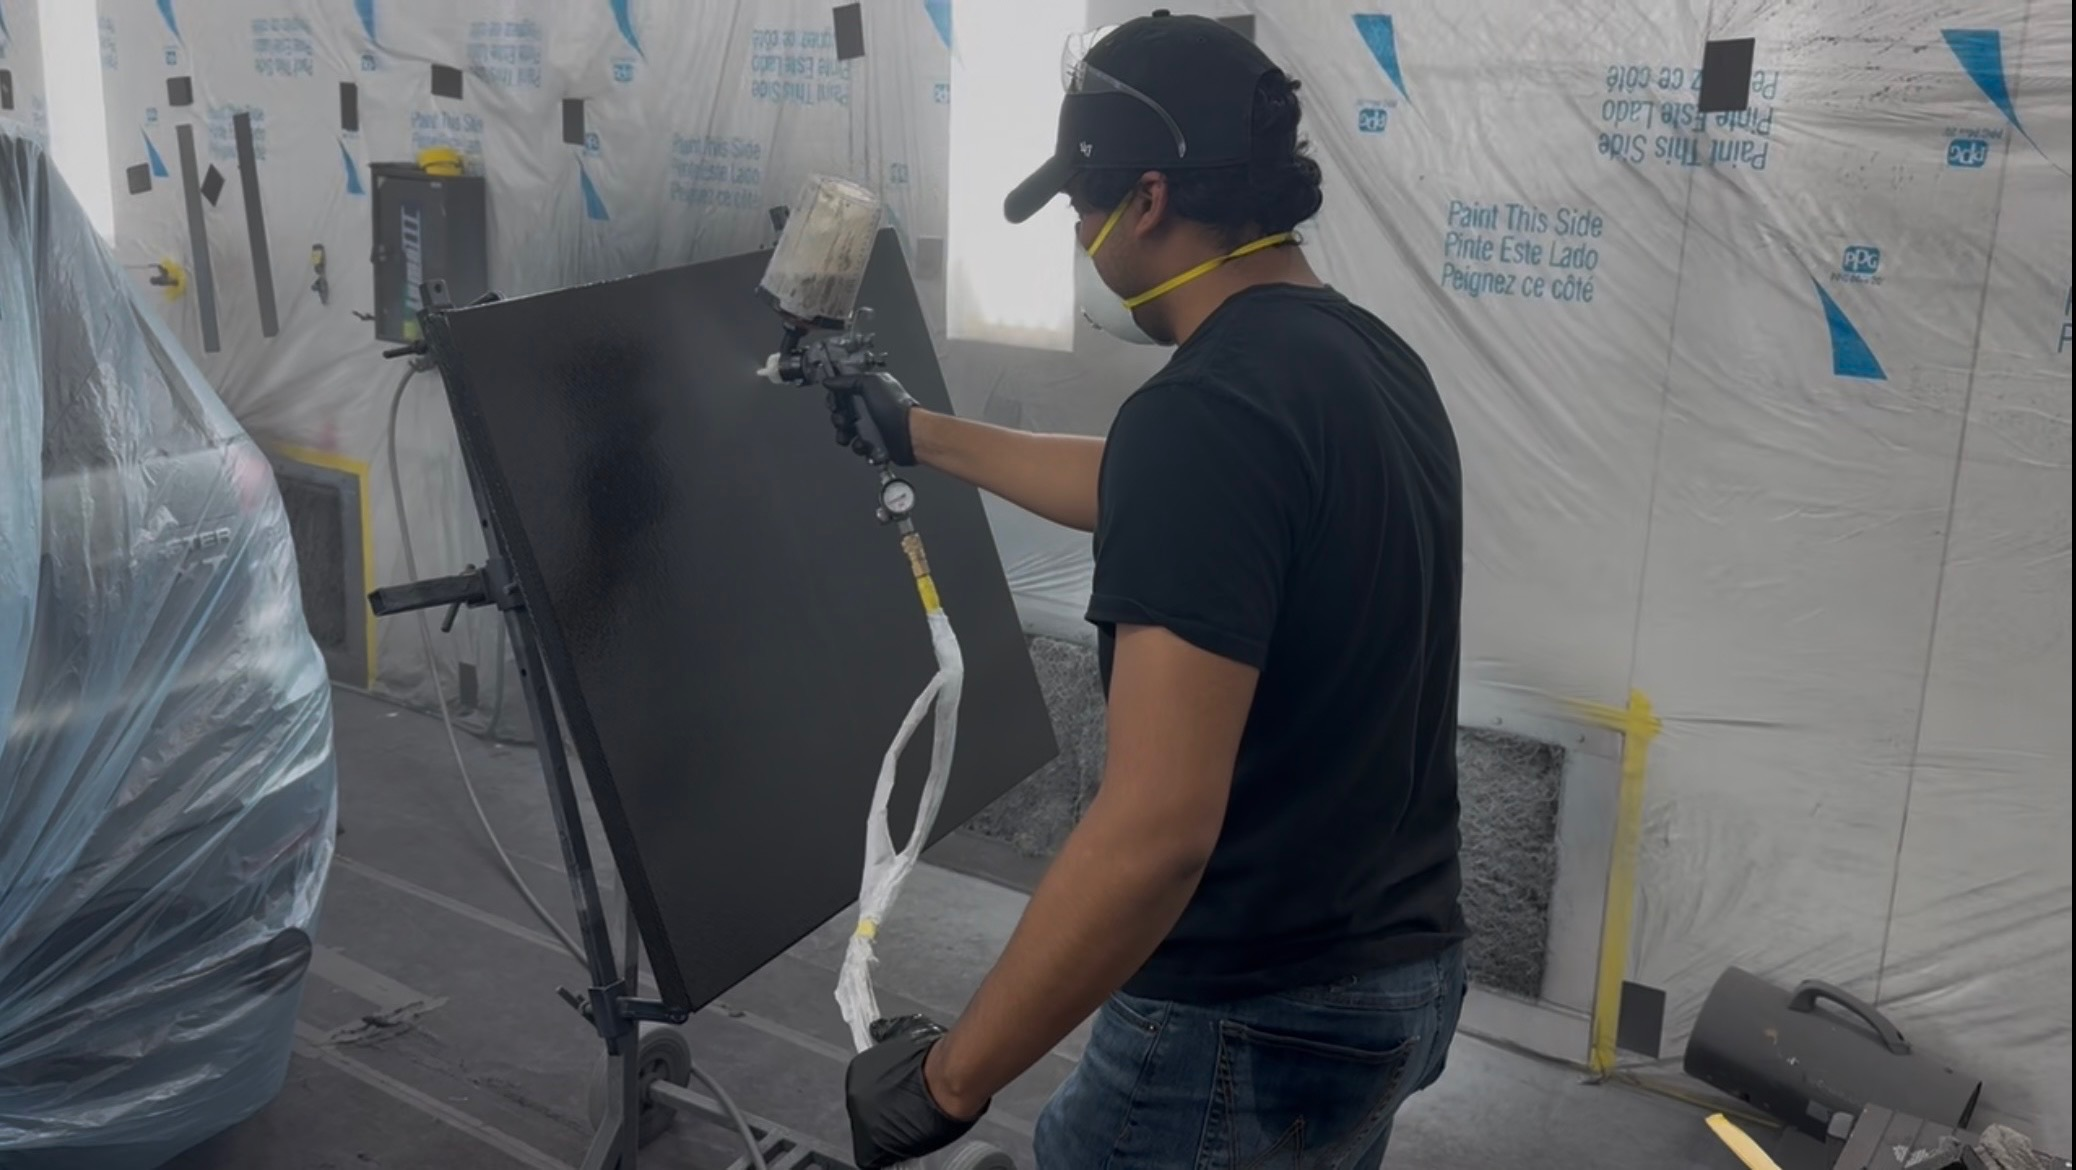
\includegraphics[
        width=2.35in,
        height=1.40in,
        keepaspectratio
    ]{spraying_topcoat}
};
\draw[RuleGray,line width=0.55pt,rounded corners=4pt]
    ($(current page.north west)+(3.10in,-1.91in)$)
    rectangle
    ($(current page.north west)+(5.65in,-3.40in)$);

% Image 3
\node[anchor=center,inner sep=0pt]
at ($(current page.north west)+(7.045in,-2.655in)$)
{
    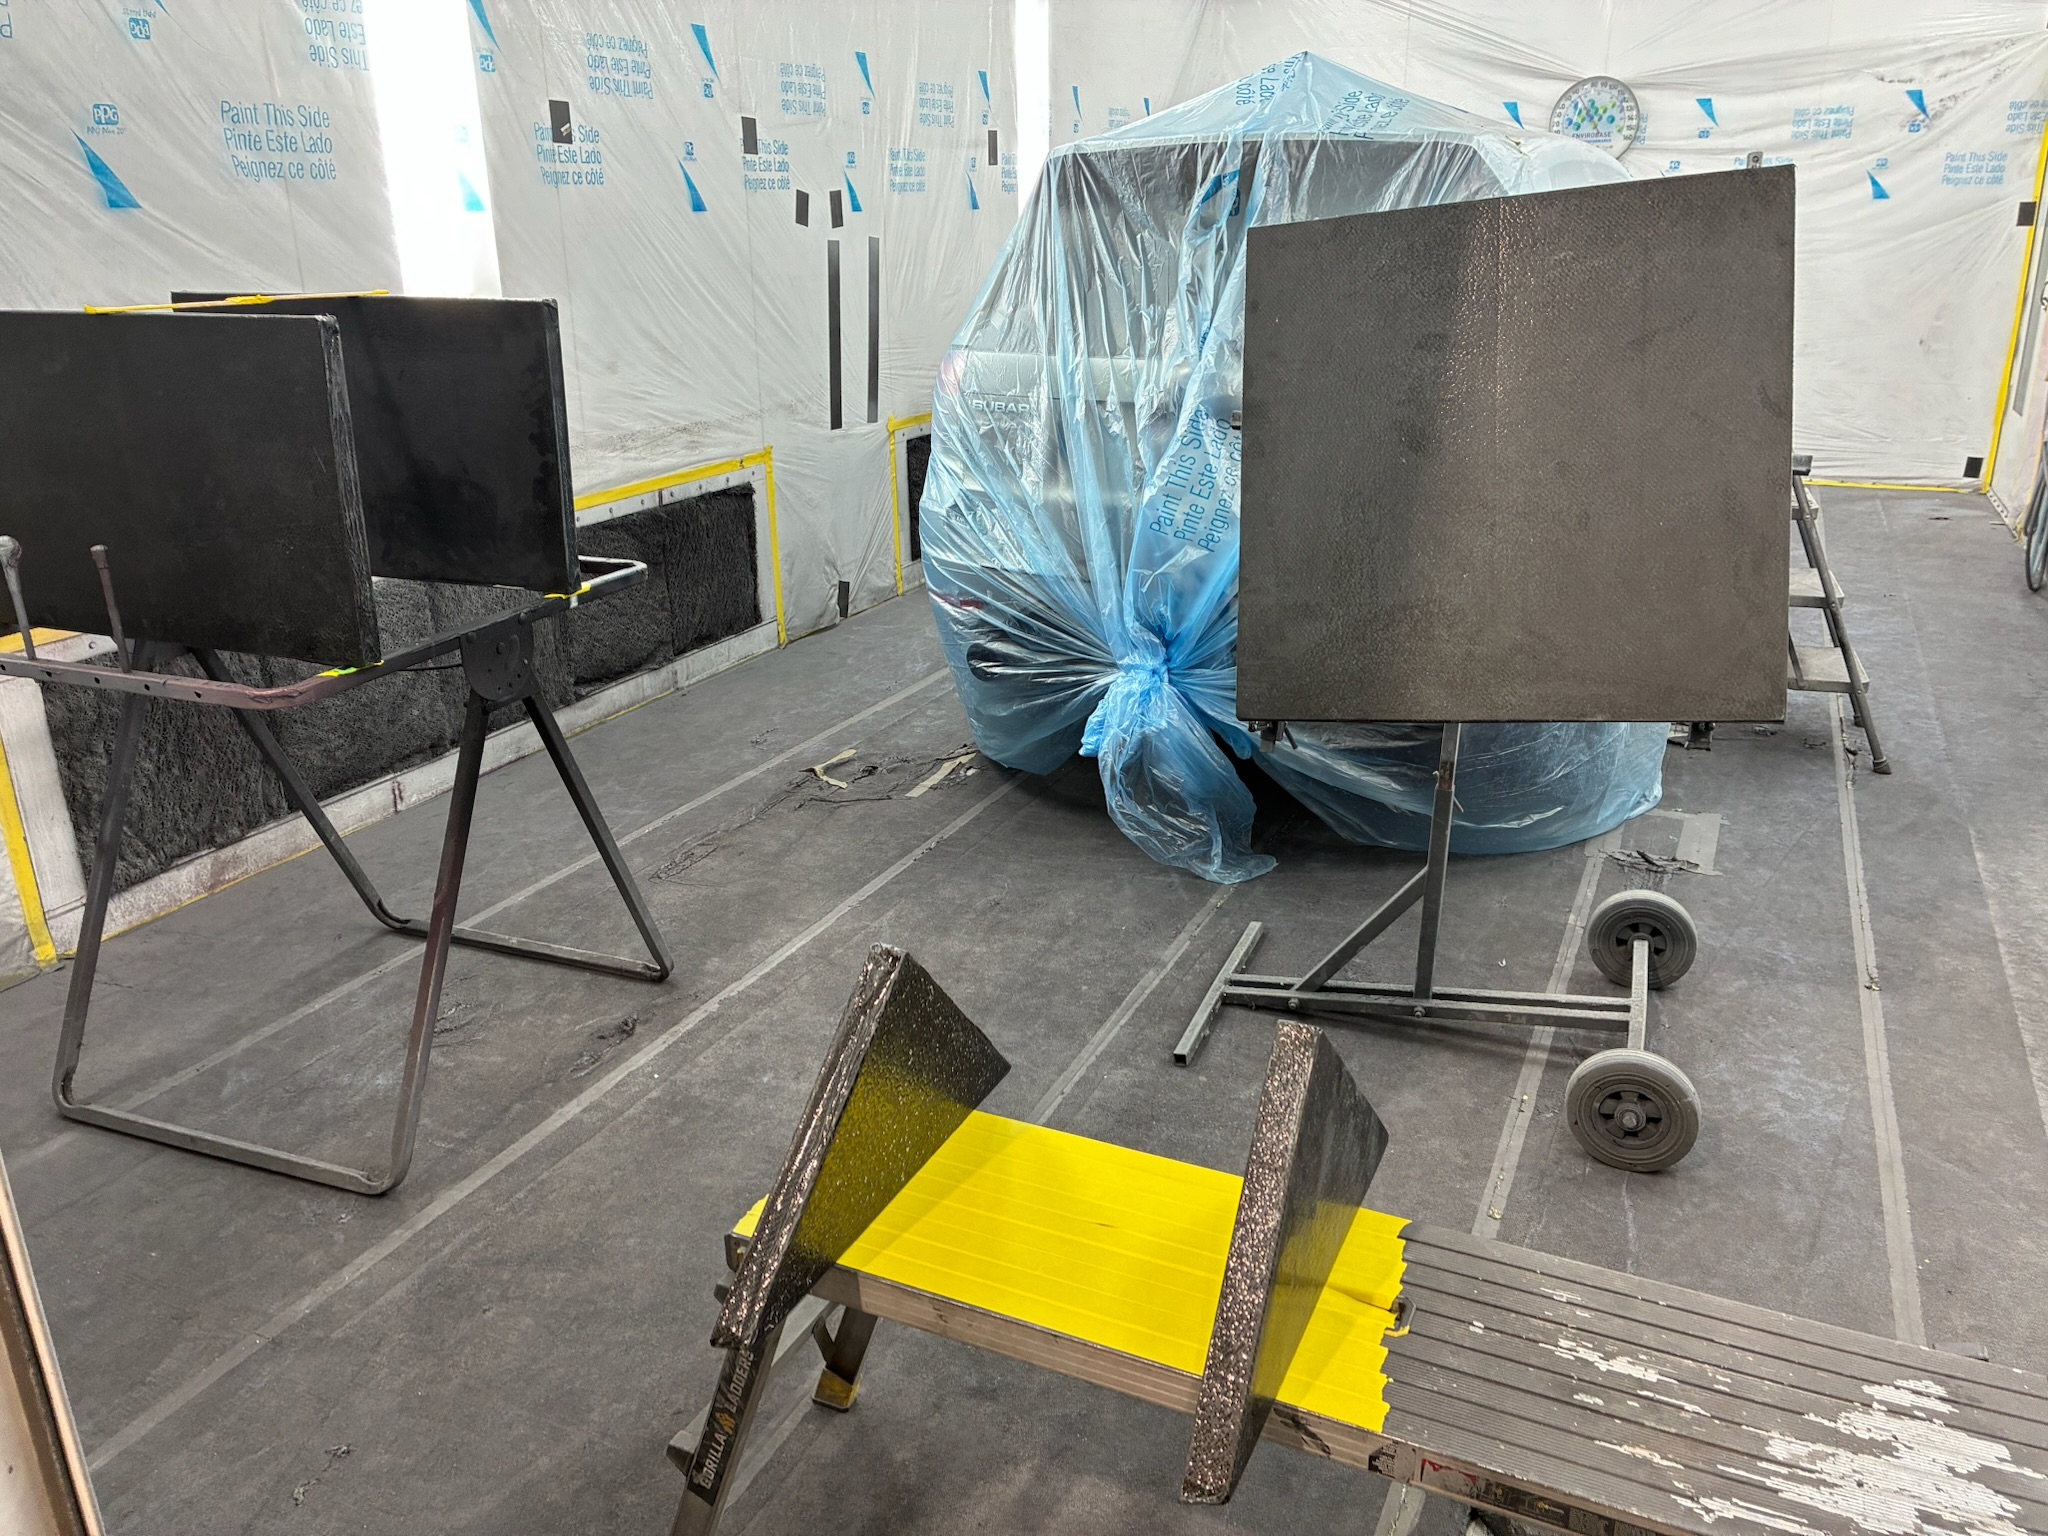
\includegraphics[
        width=2.35in,
        height=1.40in,
        keepaspectratio
    ]{topcoat_setup_apparatus}
};
\draw[RuleGray,line width=0.55pt,rounded corners=4pt]
    ($(current page.north west)+(5.77in,-1.91in)$)
    rectangle
    ($(current page.north west)+(8.32in,-3.40in)$);

% Image 4
\node[anchor=center,inner sep=0pt]
at ($(current page.north west)+(9.50in,-2.655in)$)
{
    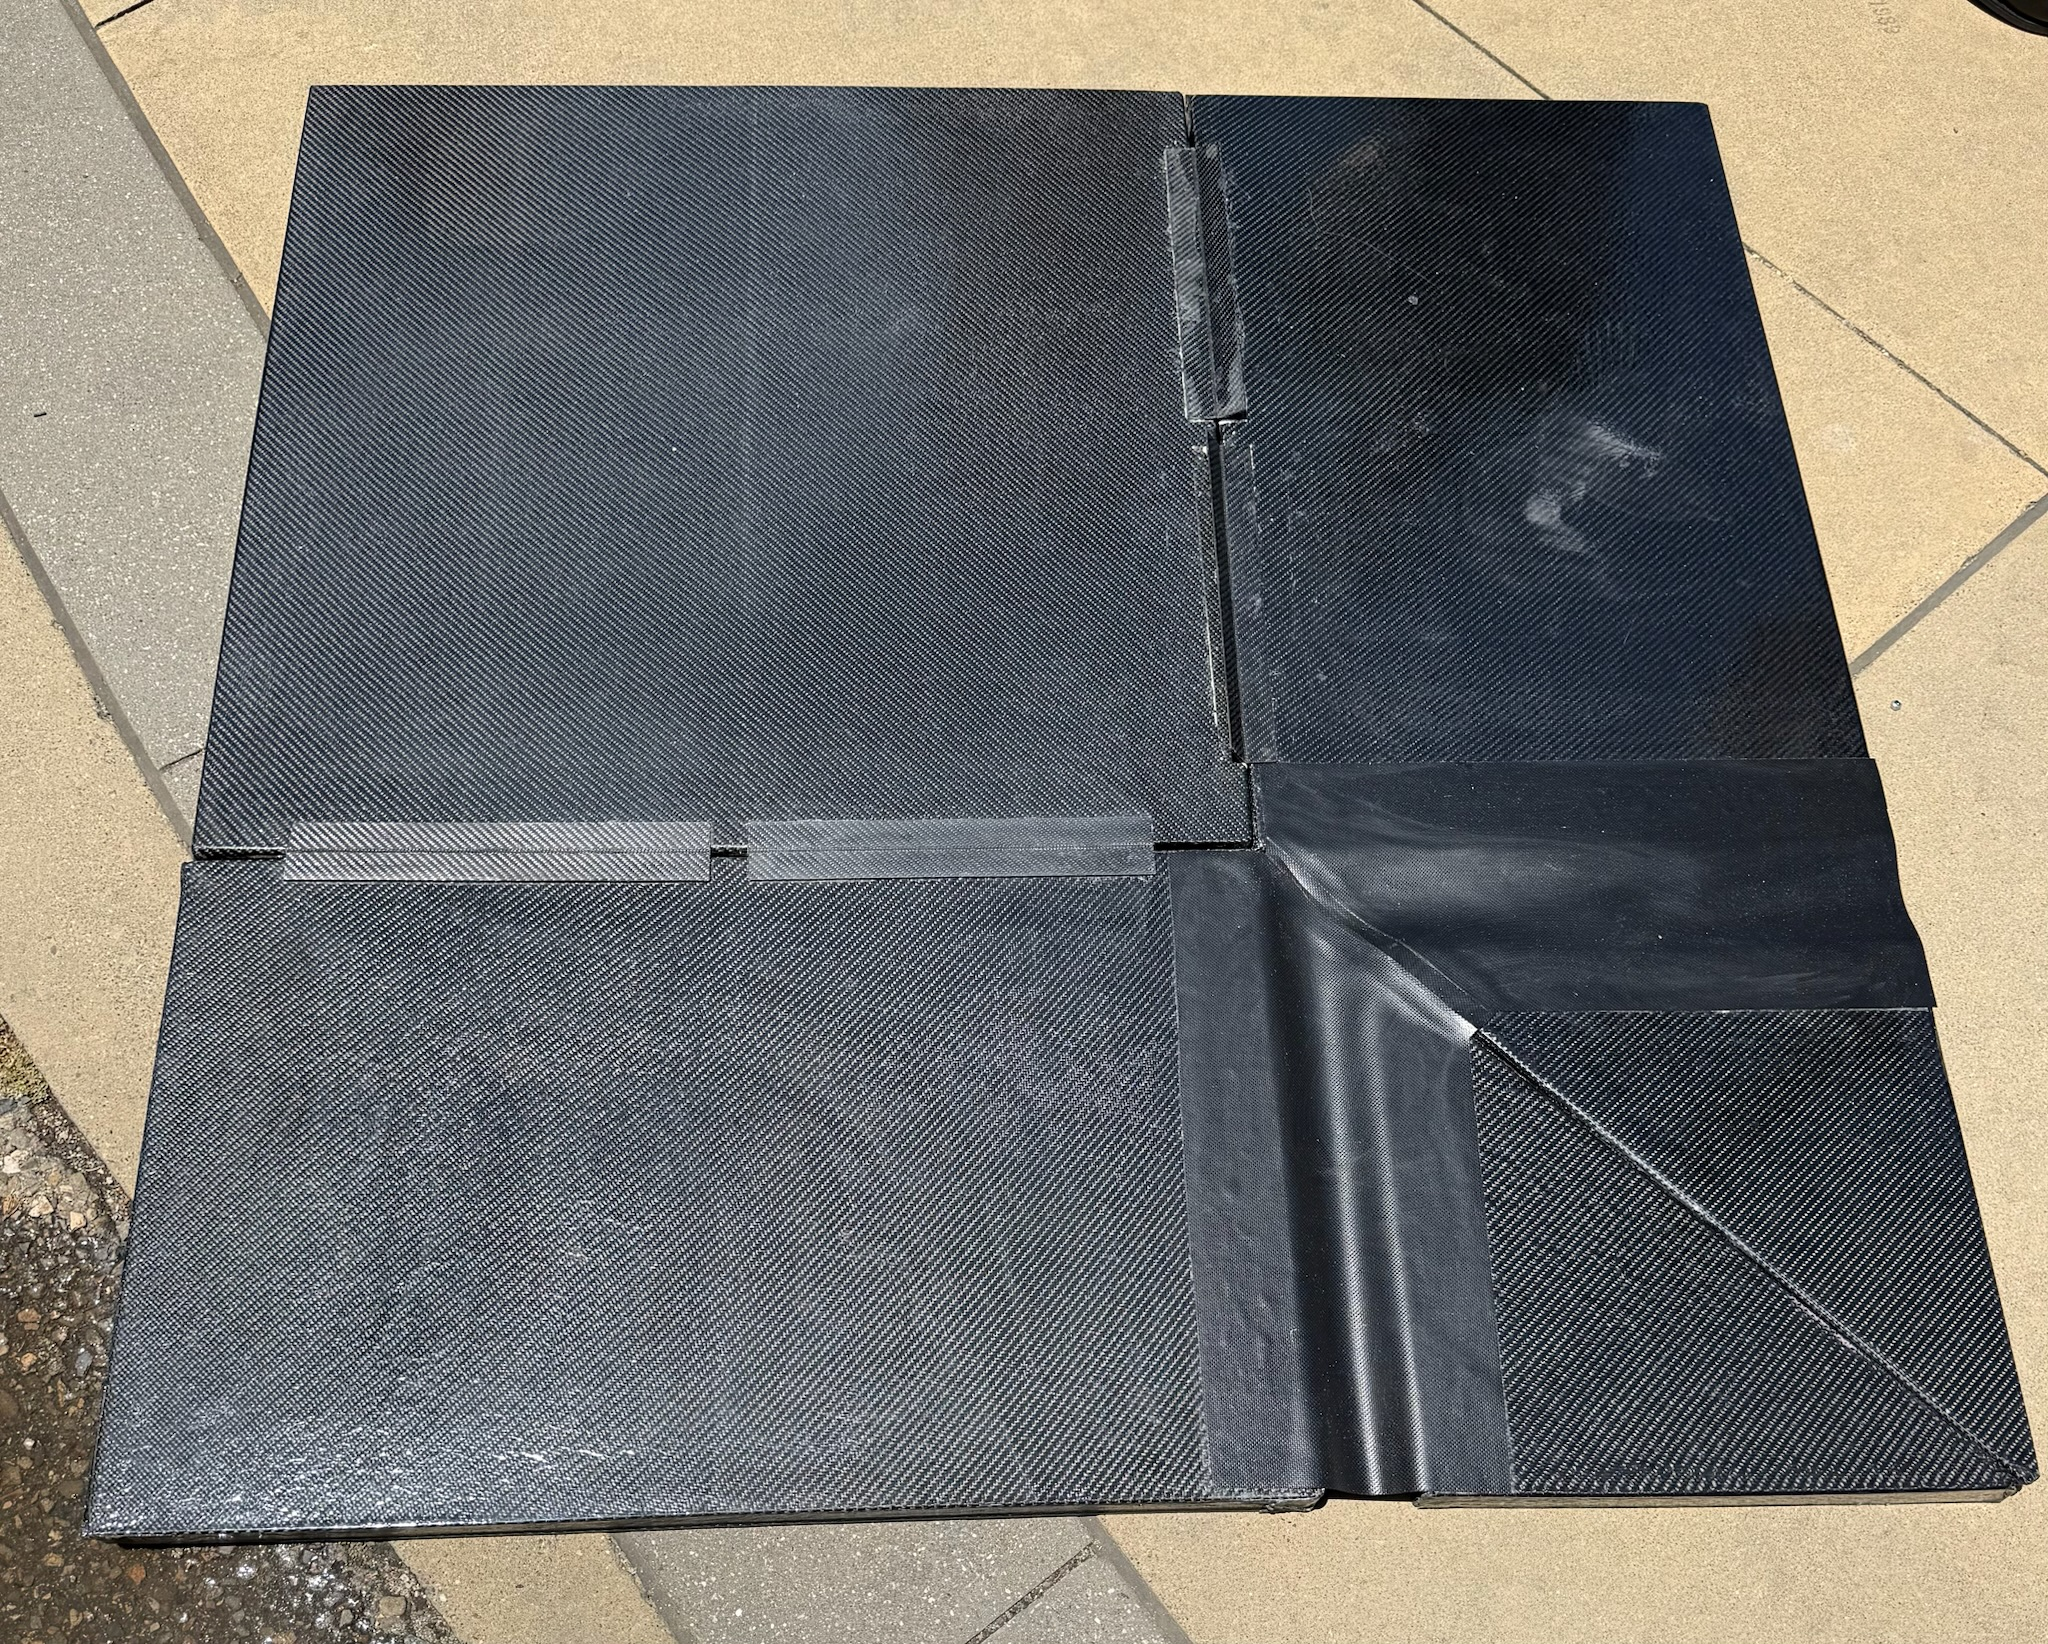
\includegraphics[
        width=2.35in,
        height=1.40in,
        keepaspectratio
    ]{refined_final_toro_cover_partial_carbon_model}
};
\draw[RuleGray,line width=0.55pt,rounded corners=4pt]
    ($(current page.north west)+(8.44in,-1.91in)$)
    rectangle
    ($(current page.north east)+(-0.42in,-3.40in)$);

% Captions
\node[anchor=north,text=Muted,font=\sffamily\fontsize{6.7}{7.3}\selectfont]
at ($(current page.north west)+(1.705in,-3.45in)$)
{Topcoat material preparation};

\node[anchor=north,text=Muted,font=\sffamily\fontsize{6.7}{7.3}\selectfont]
at ($(current page.north west)+(4.375in,-3.45in)$)
{Automotive-booth topcoat application};

\node[anchor=north,text=Muted,font=\sffamily\fontsize{6.7}{7.3}\selectfont]
at ($(current page.north west)+(7.045in,-3.45in)$)
{Coated panels drying after application};

\node[anchor=north,text=Muted,font=\sffamily\fontsize{6.7}{7.3}\selectfont]
at ($(current page.north west)+(9.50in,-3.45in)$)
{Partial carbon manufacturing model};

% Environmental rationale
\fill[SoftGold,rounded corners=4pt]
    ($(current page.north west)+(0.43in,-3.73in)$)
    rectangle
    ($(current page.north east)+(-0.42in,-4.76in)$);

\node[
    anchor=north west,
    align=left,
    text width=9.75in,
    text=Ink,
    font=\fontsize{7.05}{8.25}\selectfont
]
at ($(current page.north west)+(0.65in,-3.89in)$)
{
Because the sponsor required a carbon-fiber cover for outdoor use near chlorinated water,
environmental protection became a functional requirement rather than a cosmetic finish.
I selected and personally sprayed a UV-resistant Sunshield topcoat to seal minor laminate
porosity, reduce moisture ingress, preserve the carbon appearance, limit UV degradation of
the epoxy matrix, and isolate the composite surface from nearby metallic hardware.
};

% Results title
\node[
    anchor=north west,
    text=DeepGreen,
    font=\sffamily\bfseries\fontsize{8.0}{8.7}\selectfont
]
at ($(current page.north west)+(0.43in,-4.94in)$)
{FUNCTIONAL PROTOTYPE RESULTS};

% ------------------------------------------------------------
% Matched lower panels — larger type and improved allocation
% ------------------------------------------------------------

% Left results panel
\fill[SoftGreen,rounded corners=5pt]
    ($(current page.north west)+(0.43in,-5.22in)$)
    rectangle
    ($(current page.north west)+(5.98in,-7.39in)$);

\draw[RuleGray,line width=0.65pt,rounded corners=5pt]
    ($(current page.north west)+(0.43in,-5.22in)$)
    rectangle
    ($(current page.north west)+(5.98in,-7.39in)$);

\fill[DeepGreen,rounded corners=5pt]
    ($(current page.north west)+(0.43in,-5.22in)$)
    rectangle
    ($(current page.north west)+(5.98in,-5.58in)$);

\fill[DeepGreen]
    ($(current page.north west)+(0.43in,-5.40in)$)
    rectangle
    ($(current page.north west)+(5.98in,-5.58in)$);

\node[anchor=west,text=white,
      font=\sffamily\bfseries\fontsize{7.0}{7.6}\selectfont]
at ($(current page.north west)+(0.66in,-5.40in)$)
{SPECIFICATION};

\node[anchor=west,text=white,
      font=\sffamily\bfseries\fontsize{7.0}{7.6}\selectfont]
at ($(current page.north west)+(3.02in,-5.40in)$)
{RESULT};

\node[anchor=east,text=white,
      font=\sffamily\bfseries\fontsize{7.0}{7.6}\selectfont]
at ($(current page.north west)+(5.55in,-5.40in)$)
{STATUS};

\node[
    anchor=north west,
    align=left,
    text width=2.15in,
    text=Ink,
    font=\bfseries\fontsize{7.15}{8.55}\selectfont
]
at ($(current page.north west)+(0.66in,-5.72in)$)
{
Deployment time\\[3.4pt]
Removal time\\[3.4pt]
Single-user operation\\[3.4pt]
Single-side operation\\[3.4pt]
Deployment steps\\[3.4pt]
Removal steps\\[3.4pt]
Weight\\[3.4pt]
Folded storage
};

\node[
    anchor=north west,
    align=left,
    text width=1.45in,
    text=Ink,
    font=\fontsize{7.15}{8.55}\selectfont
]
at ($(current page.north west)+(3.02in,-5.72in)$)
{
25.51 seconds\\[3.4pt]
37.22 seconds\\[3.4pt]
100\% successful\\[3.4pt]
75\% successful\\[3.4pt]
6.4 average\\[3.4pt]
9 average\\[3.4pt]
17 lb\\[3.4pt]
2.9' x 2.9' x 1.7'
};

\node[
    anchor=north east,
    align=right,
    text width=1.05in,
    text=DeepGreen,
    font=\sffamily\bfseries\fontsize{7.05}{8.55}\selectfont
]
at ($(current page.north west)+(5.55in,-5.72in)$)
{
PASS\\[3.4pt]
PASS\\[3.4pt]
PASS\\[3.4pt]
NEAR TARGET\\[3.4pt]
PASS\\[3.4pt]
PASS\\[3.4pt]
NEAR TARGET\\[3.4pt]
PASS
};

% Right takeaways panel — widened for easier reading
\fill[SoftGreen,rounded corners=5pt]
    ($(current page.north west)+(6.14in,-5.22in)$)
    rectangle
    ($(current page.north east)+(-0.42in,-7.39in)$);

\draw[RuleGray,line width=0.65pt,rounded corners=5pt]
    ($(current page.north west)+(6.14in,-5.22in)$)
    rectangle
    ($(current page.north east)+(-0.42in,-7.39in)$);

\fill[DeepGreen,rounded corners=5pt]
    ($(current page.north west)+(6.14in,-5.22in)$)
    rectangle
    ($(current page.north east)+(-0.42in,-5.58in)$);

\fill[DeepGreen]
    ($(current page.north west)+(6.14in,-5.40in)$)
    rectangle
    ($(current page.north east)+(-0.42in,-5.58in)$);

\node[anchor=west,text=white,
      font=\sffamily\bfseries\fontsize{7.1}{7.7}\selectfont]
at ($(current page.north west)+(6.38in,-5.40in)$)
{ENGINEERING TAKEAWAYS};

\node[
    anchor=north west,
    align=left,
    text width=4.02in,
    text=Ink,
    font=\fontsize{6.75}{7.85}\selectfont
]
at ($(current page.north west)+(6.38in,-5.72in)$)
{
\textbf{Manufacturing first.}
Composite manufacturing constraints should guide the product architecture from the beginning.\\[4.5pt]
\textbf{Prioritize deliberately.}
Competing requirements must be balanced intentionally instead of maximizing every objective.\\[4.5pt]
\textbf{Lead through the process.}
Clear procedures, calm communication, and respect for teammates' strengths were essential during fabrication.\\[4.5pt]
\textbf{Next iteration.}
Reduce weight, refine the fabric-hinge fold lines, and improve panel-edge clearance.
};

% Compact concluding pathway
\node[
    anchor=center,
    align=center,
    text=PolyGold,
    font=\sffamily\bfseries\fontsize{6.3}{6.9}\selectfont
]
at ($(current page.north)+(3.06in,-7.18in)$)
{PROTOTYPE \faArrowRight\ DESIGN REFINEMENT
\faArrowRight\ REPEATABLE MANUFACTURING
\faArrowRight\ PRODUCT};

% Validation resources
\node[
    anchor=north,
    align=center,
    text=DeepGreen,
    font=\sffamily\bfseries\fontsize{6.6}{7.2}\selectfont
]
at ($(current page.north)+(0,-7.58in)$)
{\href{\ToroDeploymentLink}{\faPlayCircle\ DEPLOYMENT}
\hspace{18pt}
\href{\ToroRemovalLink}{\faPlayCircle\ REMOVAL / FOLDING}
\hspace{18pt}
\href{\ToroPosterLink}{\faFilePdf\ EXPO POSTER}
\hspace{18pt}
\href{\ToroReportLink}{\faFilePdf\ FINAL REPORT}};

% Footer
\node[
    anchor=south west,
    text=white,
    font=\sffamily\bfseries\fontsize{7.1}{7.7}\selectfont
]
at ($(current page.south west)+(0.42in,0.17in)$)
{\faArrowLeft\ MANUFACTURING-DRIVEN DESIGN};

\node[
    anchor=south,
    text=white,
    font=\sffamily\fontsize{7.0}{7.6}\selectfont
]
at ($(current page.south)+(0,0.17in)$)
{TORO COVER \hspace{6pt} 3 / 3};

\node[
    anchor=south east,
    text=white,
    font=\sffamily\bfseries\fontsize{7.1}{7.7}\selectfont
]
at ($(current page.south east)+(-0.42in,0.17in)$)
{NEXT PROJECT \faArrowRight};

\end{tikzpicture}
\input{paddle}
\clearpage
 before \end{document}.
% 3. Image references use the original Overleaf base filenames
%    without extensions.
% ============================================================



% ============================================================
% CLICKABLE PROJECT RESOURCES
% All links use the exact Google Drive resources supplied.
% ============================================================
\providecommand{\ToroDrawingLink}{https://drive.google.com/file/d/1A7-7wMnRNLuQDaTgxeuUCBsGNqyXzOGV/view?usp=sharing}
\providecommand{\ToroDimensionsLink}{https://drive.google.com/file/d/13sw3BNJvE8GdzlRffxoF2n5r9Gzxide7/view?usp=sharing}
\providecommand{\ToroProblemLink}{https://drive.google.com/file/d/1zHtl8zrb13F1yeN74ptawpfS5UM_xsuw/view?usp=drive_link}
\providecommand{\ToroReportLink}{https://drive.google.com/file/d/1ULZ-P46lFsC2x29ZfmRVIKgYnr9o8hMt/view?usp=drive_link}
\providecommand{\ToroPosterLink}{https://drive.google.com/file/d/1vKiKaJUcHQb_db-FkZnRF6EvtuM4hKyS/view?usp=drive_link}
\providecommand{\ToroDeploymentLink}{https://drive.google.com/file/d/1XJx34o80_mZPTl7xy93HtWAgtS3ThhvY/view?usp=drive_link}
\providecommand{\ToroRemovalLink}{https://drive.google.com/file/d/1O7xYeyB67NUwT-j1B1HeiCcHnZDYjk6_/view?usp=drive_link}

% ============================================================
% PAGE 1 — PROJECT OVERVIEW, OWNERSHIP, AND ARCHITECTURE
% ============================================================

\clearpage
\thispagestyle{empty}
\hypertarget{toro}{}
\null

\begin{tikzpicture}[remember picture,overlay]

% Background
\fill[white]
    (current page.south west)
    rectangle
    (current page.north east);

% Page bars
\fill[DeepGreen]
    (current page.north west)
    rectangle
    ($(current page.north east)+(0,-0.095in)$);

\fill[PolyGold]
    ($(current page.north west)+(0,-0.095in)$)
    rectangle
    ($(current page.north east)+(0,-0.14in)$);

\fill[DeepGreen]
    (current page.south west)
    rectangle
    ($(current page.south east)+(0,0.36in)$);

\fill[PolyGold]
    ($(current page.south west)+(0,0.36in)$)
    rectangle
    ($(current page.south east)+(0,0.405in)$);

% Header
\node[
    anchor=north west,
    text=PolyGold,
    font=\sffamily\bfseries\fontsize{8.1}{8.7}\selectfont
]
at ($(current page.north west)+(0.42in,-0.39in)$)
{01 COMPOSITES \hspace{5pt}/\hspace{5pt} PROJECT 01};

\node[
    anchor=north west,
    text=DeepGreen,
    font=\bfseries\fontsize{23.5}{24.5}\selectfont
]
at ($(current page.north west)+(0.40in,-0.67in)$)
{TORO CARBON FIBER SAFETY COVER};

\node[
    anchor=north west,
    text=Muted,
    font=\sffamily\fontsize{8.4}{9.2}\selectfont
]
at ($(current page.north west)+(0.42in,-1.12in)$)
{Cal Poly Composites Laboratory \hspace{7pt}\textbullet\hspace{7pt}
Team Project \hspace{7pt}\textbullet\hspace{7pt}
Fall--Spring 2026 \hspace{7pt}\textbullet\hspace{7pt}
San Luis Obispo, California};

\fill[PolyGold]
    ($(current page.north west)+(0.42in,-1.37in)$)
    rectangle
    ($(current page.north west)+(6.1in,-1.325in)$);

% Challenge text
\node[
    anchor=north west,
    text=DeepGreen,
    font=\sffamily\bfseries\fontsize{8.1}{8.8}\selectfont
]
at ($(current page.north west)+(0.43in,-1.61in)$)
{THE CHALLENGE};

\node[
    anchor=north west,
    align=left,
    text width=4.47in,
    text=Ink,
    font=\fontsize{8.05}{9.65}\selectfont
]
at ($(current page.north west)+(0.43in,-1.84in)$)
{
Develop a lightweight cover for a 6 ft by 6 ft in-ground spa
that could be deployed by one person, stored compactly,
provide insulation, resist a poolside environment, and maintain
a refined appearance. The sponsor supplied an ambitious but
intentionally broad project statement, requiring the team to
define the product architecture, priorities, manufacturing
strategy, and realistic path toward future commercialization.
};

% Role box
\fill[SoftGold,rounded corners=5pt]
    ($(current page.north west)+(0.42in,-2.88in)$)
    rectangle
    ($(current page.north west)+(4.98in,-4.58in)$);

\fill[PolyGold]
    ($(current page.north west)+(0.42in,-2.88in)$)
    rectangle
    ($(current page.north west)+(0.52in,-4.58in)$);

\node[
    anchor=north west,
    text=DeepGreen,
    font=\sffamily\bfseries\fontsize{8.1}{8.8}\selectfont
]
at ($(current page.north west)+(0.66in,-3.02in)$)
{MY ROLE — DESIGN \& MANUFACTURING LEAD};

\node[
    anchor=north west,
    align=left,
    text width=4.02in,
    text=Ink,
    font=\fontsize{7.05}{8.15}\selectfont
]
at ($(current page.north west)+(0.66in,-3.27in)$)
{
\textbullet\ Modeled every custom part and the complete assembly\\[1.5pt]
\textbullet\ Produced the engineering drawing package independently\\[1.5pt]
\textbullet\ Developed the composite-panel manufacturing process\\[1.5pt]
\textbullet\ Created all waterjet DXFs and manufacturing geometry\\[1.5pt]
\textbullet\ Trained teammates in wet layup and vacuum bagging\\[1.5pt]
\textbullet\ Presented feasibility, scope, and tradeoffs to the sponsor
};

% Large deployed foam-model image
\node[anchor=center,inner sep=0pt]
at ($(current page.north west)+(8.00in,-3.04in)$)
{
    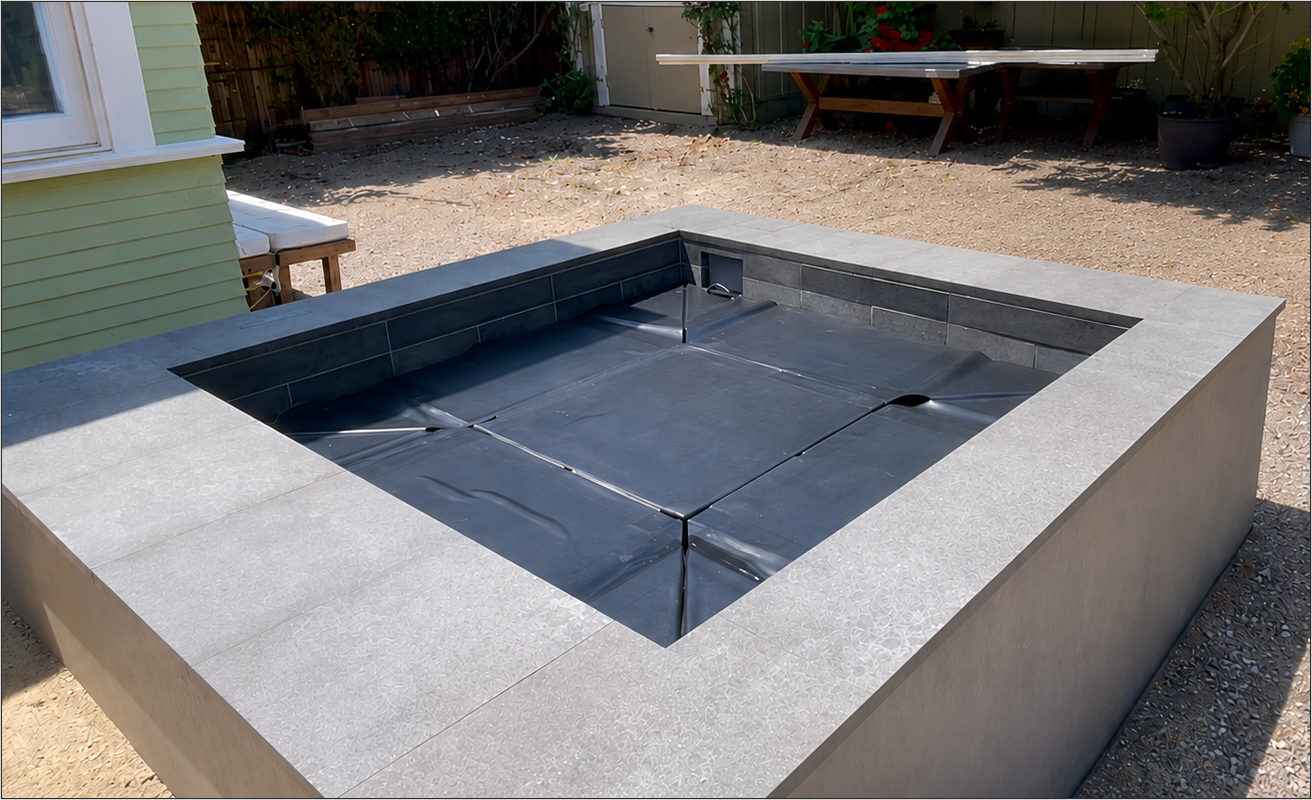
\includegraphics[
        width=5.55in,
        height=2.78in,
        keepaspectratio
    ]{deployed_functional_prototype}
};

\draw[DeepGreen,line width=0.8pt,rounded corners=7pt]
    ($(current page.north west)+(5.16in,-1.61in)$)
    rectangle
    ($(current page.north east)+(-0.42in,-4.47in)$);

\node[
    anchor=north west,
    text=Muted,
    font=\sffamily\fontsize{6.2}{6.9}\selectfont
]
at ($(current page.north west)+(5.18in,-4.54in)$)
{Functional foam model deployed over the sponsor's in-ground spa.};

% Image-strip title
\node[
    anchor=north west,
    text=DeepGreen,
    font=\sffamily\bfseries\fontsize{8.1}{8.8}\selectfont
]
at ($(current page.north west)+(0.43in,-4.78in)$)
{PRODUCT DEVELOPMENT AND FINAL ARCHITECTURE};

% Five-image development strip — CAD-first sequence
% Image 1: topside CAD
\node[anchor=center,inner sep=0pt]
at ($(current page.north west)+(1.47in,-5.73in)$)
{
    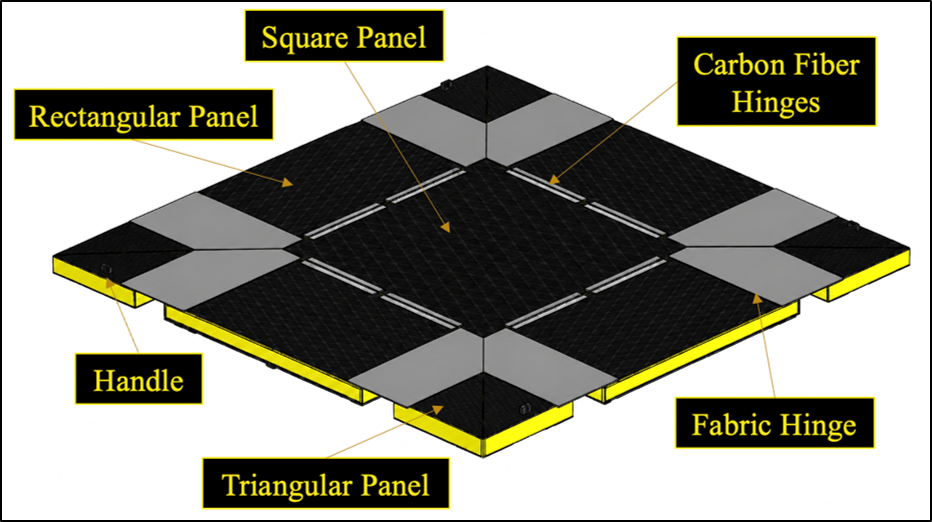
\includegraphics[
        width=1.92in,
        height=1.30in,
        keepaspectratio
    ]{Toro_Cover_topside_Cad}
};
\draw[RuleGray,line width=0.55pt,rounded corners=4pt]
    ($(current page.north west)+(0.43in,-5.04in)$)
    rectangle
    ($(current page.north west)+(2.51in,-6.43in)$);

% Image 2: underside CAD
\node[anchor=center,inner sep=0pt]
at ($(current page.north west)+(3.66in,-5.73in)$)
{
    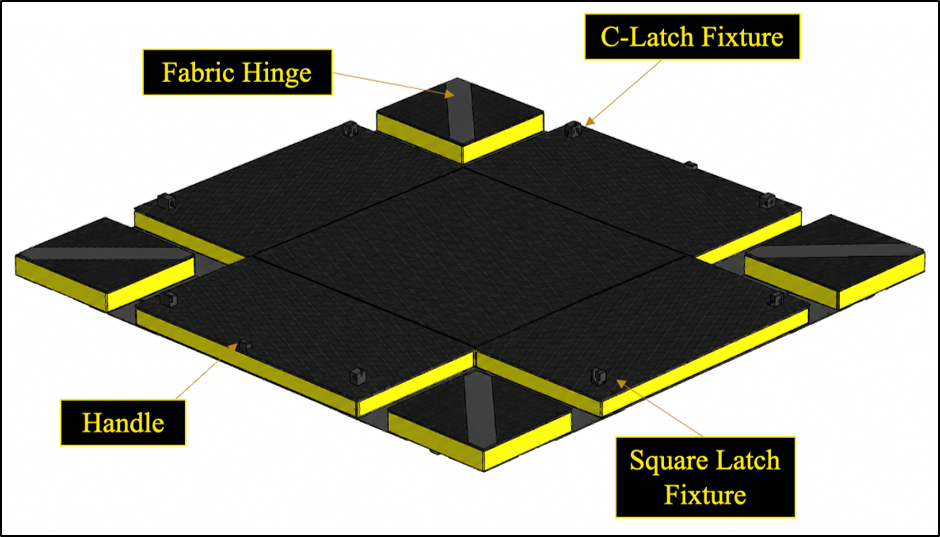
\includegraphics[
        width=1.92in,
        height=1.30in,
        keepaspectratio
    ]{toro_cover_underside_cad}
};
\draw[RuleGray,line width=0.55pt,rounded corners=4pt]
    ($(current page.north west)+(2.62in,-5.04in)$)
    rectangle
    ($(current page.north west)+(4.70in,-6.43in)$);

% Image 3: folded CAD
\node[anchor=center,inner sep=0pt]
at ($(current page.north west)+(5.85in,-5.73in)$)
{
    \includegraphics[
        width=1.92in,
        height=1.30in,
        keepaspectratio
    ]{\detokenize{Toro_Cover_folded Configuration}}
};
\draw[RuleGray,line width=0.55pt,rounded corners=4pt]
    ($(current page.north west)+(4.81in,-5.04in)$)
    rectangle
    ($(current page.north west)+(6.89in,-6.43in)$);

% Image 4: dual-use product concept
\node[anchor=center,inner sep=0pt]
at ($(current page.north west)+(8.04in,-5.73in)$)
{
    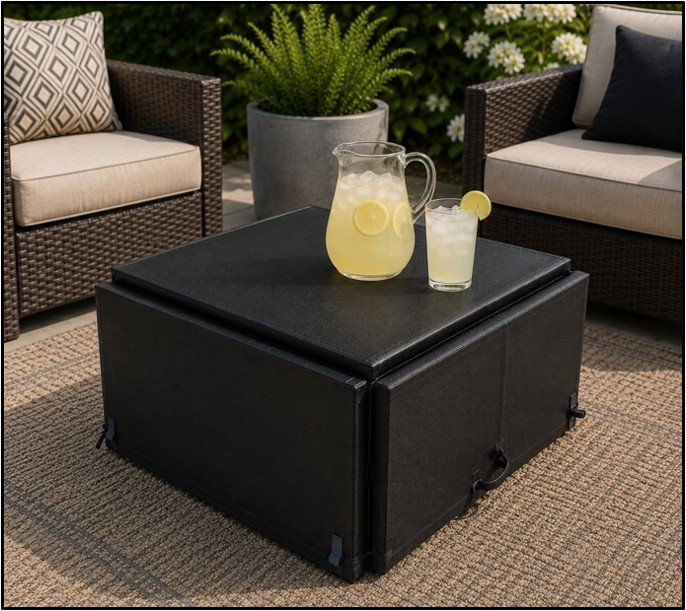
\includegraphics[
        width=1.92in,
        height=1.30in,
        keepaspectratio
    ]{generative_AI_concept_toro_cover_art}
};
\draw[RuleGray,line width=0.55pt,rounded corners=4pt]
    ($(current page.north west)+(7.00in,-5.04in)$)
    rectangle
    ($(current page.north west)+(9.08in,-6.43in)$);

% Image 5: folded foam functional prototype
% The portrait photograph is deliberately clipped to the landscape frame
% so the ottoman fills the card without extending beyond its border.
\begin{scope}
\clip[rounded corners=4pt]
    ($(current page.north west)+(9.19in,-5.04in)$)
    rectangle
    ($(current page.north east)+(-0.43in,-6.43in)$);

% Keep the original image proportions and center it within the existing card.
\node[anchor=center,inner sep=0pt]
at ($(current page.north west)+(9.88in,-5.735in)$)
{
    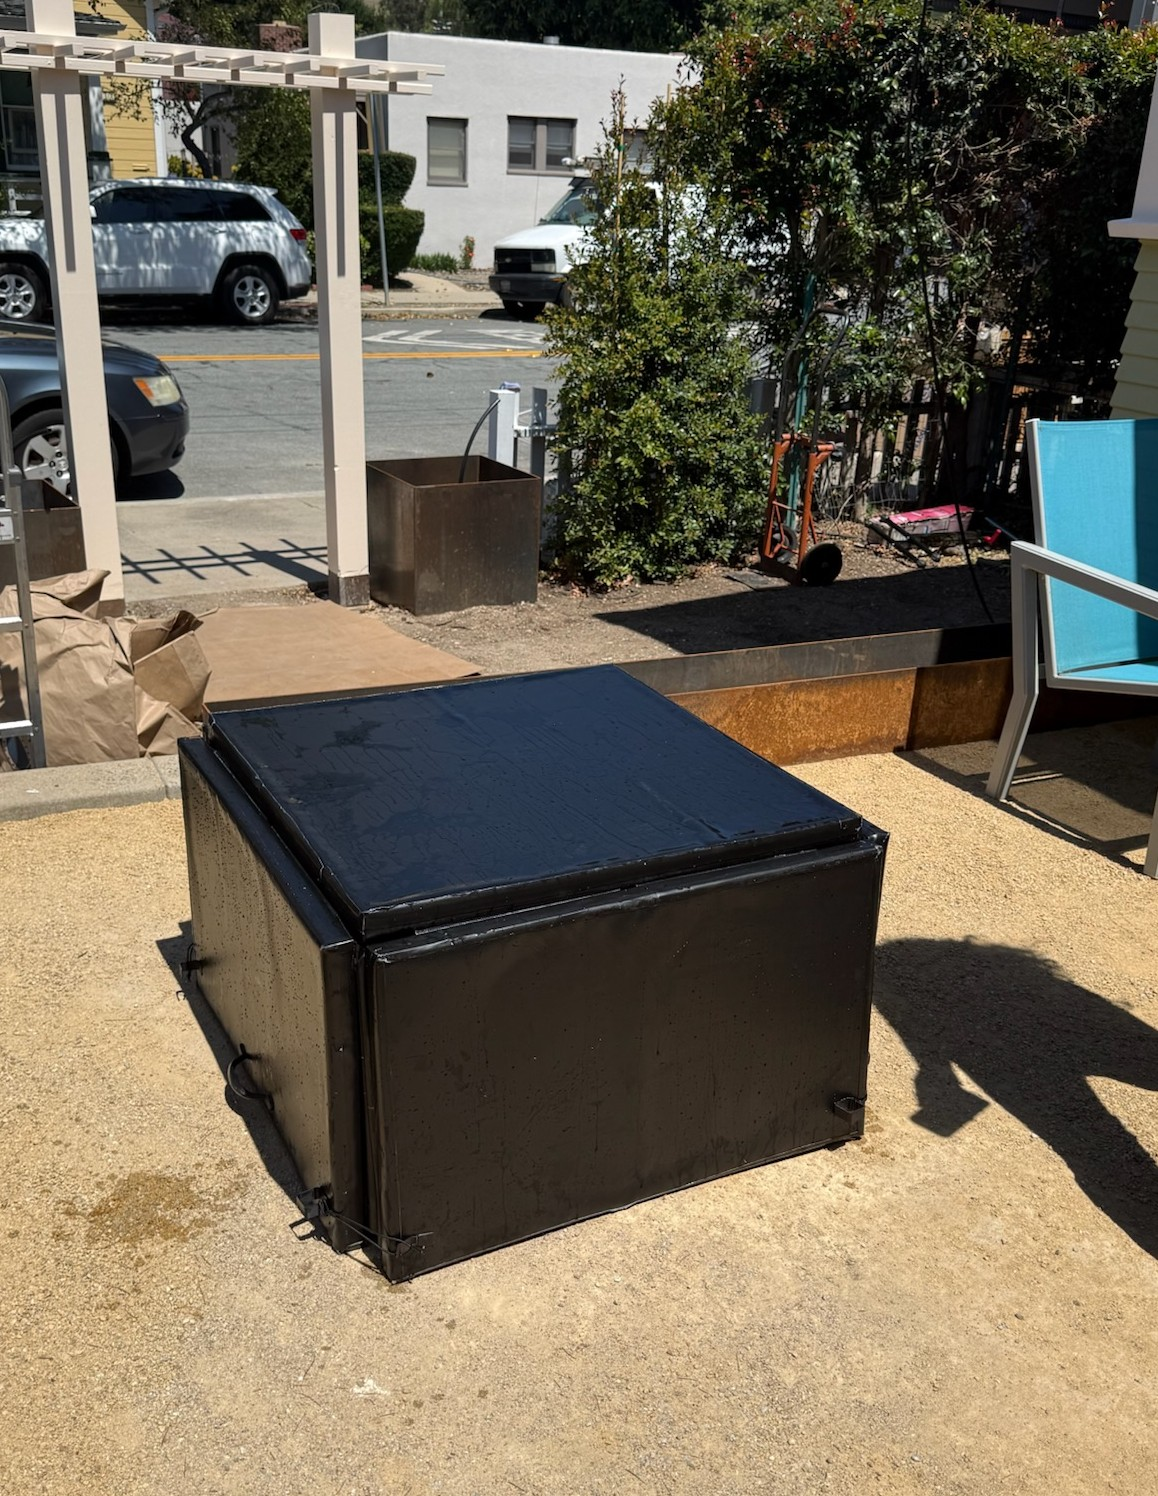
\includegraphics[
        width=1.58in,
        height=1.28in,
        keepaspectratio
    ]{foam_model_folded_backyard_image}
};
\end{scope}

\draw[RuleGray,line width=0.55pt,rounded corners=4pt]
    ($(current page.north west)+(9.19in,-5.04in)$)
    rectangle
    ($(current page.north east)+(-0.43in,-6.43in)$);

% Larger captions
\node[anchor=north,align=center,text width=1.95in,text=Muted,
      font=\sffamily\fontsize{6.8}{7.4}\selectfont]
at ($(current page.north west)+(1.47in,-6.49in)$)
{Topside panel architecture};

\node[anchor=north,align=center,text width=1.95in,text=Muted,
      font=\sffamily\fontsize{6.8}{7.4}\selectfont]
at ($(current page.north west)+(3.66in,-6.49in)$)
{Underside hinge architecture};

\node[anchor=north,align=center,text width=1.95in,text=Muted,
      font=\sffamily\fontsize{6.8}{7.4}\selectfont]
at ($(current page.north west)+(5.85in,-6.49in)$)
{Folded CAD configuration};

\node[anchor=north,align=center,text width=1.95in,text=Muted,
      font=\sffamily\fontsize{6.8}{7.4}\selectfont]
at ($(current page.north west)+(8.04in,-6.49in)$)
{Dual-use product vision};

\node[anchor=north,align=center,text width=1.95in,text=Muted,
      font=\sffamily\fontsize{6.8}{7.4}\selectfont]
at ($(current page.north west)+(9.88in,-6.49in)$)
{Folded foam prototype};

% Page 1 resource bar — centered and non-repeated resources
\fill[Panel,rounded corners=4pt]
    ($(current page.north west)+(0.43in,-7.05in)$)
    rectangle
    ($(current page.north east)+(-0.43in,-7.64in)$);
\draw[RuleGray,line width=0.5pt,rounded corners=4pt]
    ($(current page.north west)+(0.43in,-7.05in)$)
    rectangle
    ($(current page.north east)+(-0.43in,-7.64in)$);

\node[
    anchor=center,
    align=center,
    text=DeepGreen,
    font=\sffamily\bfseries\fontsize{6.9}{7.5}\selectfont
]
at ($(current page.north)+(0,-7.345in)$)
{\href{\ToroDrawingLink}{\faDraftingCompass\ DRAWING PACKAGE}
\hspace{24pt}
\href{\ToroDimensionsLink}{\faImage\ DIMENSION STUDY}
\hspace{24pt}
\href{\ToroProblemLink}{\faFileImage\ PROBLEM STATEMENT}};

% Footer
\node[
    anchor=south west,
    text=white,
    font=\sffamily\bfseries\fontsize{7.1}{7.7}\selectfont
]
at ($(current page.south west)+(0.42in,0.17in)$)
{\hyperlink{composites}{\faArrowLeft\ COMPOSITES}};

\node[
    anchor=south,
    text=white,
    font=\sffamily\fontsize{7.0}{7.6}\selectfont
]
at ($(current page.south)+(0,0.17in)$)
{TORO COVER \hspace{6pt} 1 / 3};

\node[
    anchor=south east,
    text=white,
    font=\sffamily\bfseries\fontsize{7.1}{7.7}\selectfont
]
at ($(current page.south east)+(-0.42in,0.17in)$)
{MANUFACTURING-DRIVEN DESIGN \faArrowRight};

\end{tikzpicture}


% ============================================================
% PAGE 2 — MANUFACTURING-DRIVEN DESIGN
% ============================================================

\clearpage
\thispagestyle{empty}
\hypertarget{toro-manufacturing}{}
\null

\begin{tikzpicture}[remember picture,overlay]

% Background and bars
\fill[white]
    (current page.south west)
    rectangle
    (current page.north east);

\fill[DeepGreen]
    (current page.north west)
    rectangle
    ($(current page.north east)+(0,-0.095in)$);

\fill[PolyGold]
    ($(current page.north west)+(0,-0.095in)$)
    rectangle
    ($(current page.north east)+(0,-0.14in)$);

\fill[DeepGreen]
    (current page.south west)
    rectangle
    ($(current page.south east)+(0,0.36in)$);

\fill[PolyGold]
    ($(current page.south west)+(0,0.36in)$)
    rectangle
    ($(current page.south east)+(0,0.405in)$);

% Header
\node[
    anchor=north west,
    text=PolyGold,
    font=\sffamily\bfseries\fontsize{8.1}{8.7}\selectfont
]
at ($(current page.north west)+(0.42in,-0.39in)$)
{TORO COVER \hspace{5pt}/\hspace{5pt} DESIGN FOR MANUFACTURABILITY};

\node[
    anchor=north west,
    text=DeepGreen,
    font=\bfseries\fontsize{23}{24}\selectfont
]
at ($(current page.north west)+(0.40in,-0.67in)$)
{THE ENVELOPE METHOD};

\node[
    anchor=north west,
    text=Muted,
    font=\sffamily\fontsize{8.7}{9.6}\selectfont
]
at ($(current page.north west)+(0.42in,-1.12in)$)
{A one-layup process developed for unusually thick insulated composite sandwich panels};

\fill[PolyGold]
    ($(current page.north west)+(0.42in,-1.36in)$)
    rectangle
    ($(current page.north west)+(5.30in,-1.315in)$);

% Process explanation
\fill[SoftGold,rounded corners=5pt]
    ($(current page.north west)+(0.42in,-1.61in)$)
    rectangle
    ($(current page.north east)+(-0.42in,-2.90in)$);

\fill[PolyGold]
    ($(current page.north west)+(0.42in,-1.61in)$)
    rectangle
    ($(current page.north west)+(0.52in,-2.90in)$);

\node[
    anchor=north west,
    text=DeepGreen,
    font=\sffamily\bfseries\fontsize{7.9}{8.6}\selectfont
]
at ($(current page.north west)+(0.67in,-1.76in)$)
{PROCESS INNOVATION};

\node[
    anchor=north west,
    align=left,
    text width=9.55in,
    text=Ink,
    font=\fontsize{7.35}{8.75}\selectfont
]
at ($(current page.north west)+(0.67in,-2.02in)$)
{
Weight reduction and insulation were both essential, leading to the selection of an
XPS foam core. Because XPS could not tolerate composite heat-cure temperatures, prepreg
processing was not practical and the panels had to be manufactured by wet layup with a
room-temperature cure. To simplify this process, I waterjet-cut XPS perimeter strips from
excess foam and placed them around each core inside the vacuum enclosure. Under vacuum,
the top and bottom carbon skins met along the panel sides and compressed against this
border, eliminating a separate edge-banding layup and reducing corner pleating.
};

% Workflow title
\node[
    anchor=north west,
    text=DeepGreen,
    font=\sffamily\bfseries\fontsize{8.0}{8.7}\selectfont
]
at ($(current page.north west)+(0.43in,-3.06in)$)
{MANUFACTURING WORKFLOW};

% Row 1 image 1
\node[anchor=center,inner sep=0pt]
at ($(current page.north west)+(2.07in,-4.105in)$)
{
    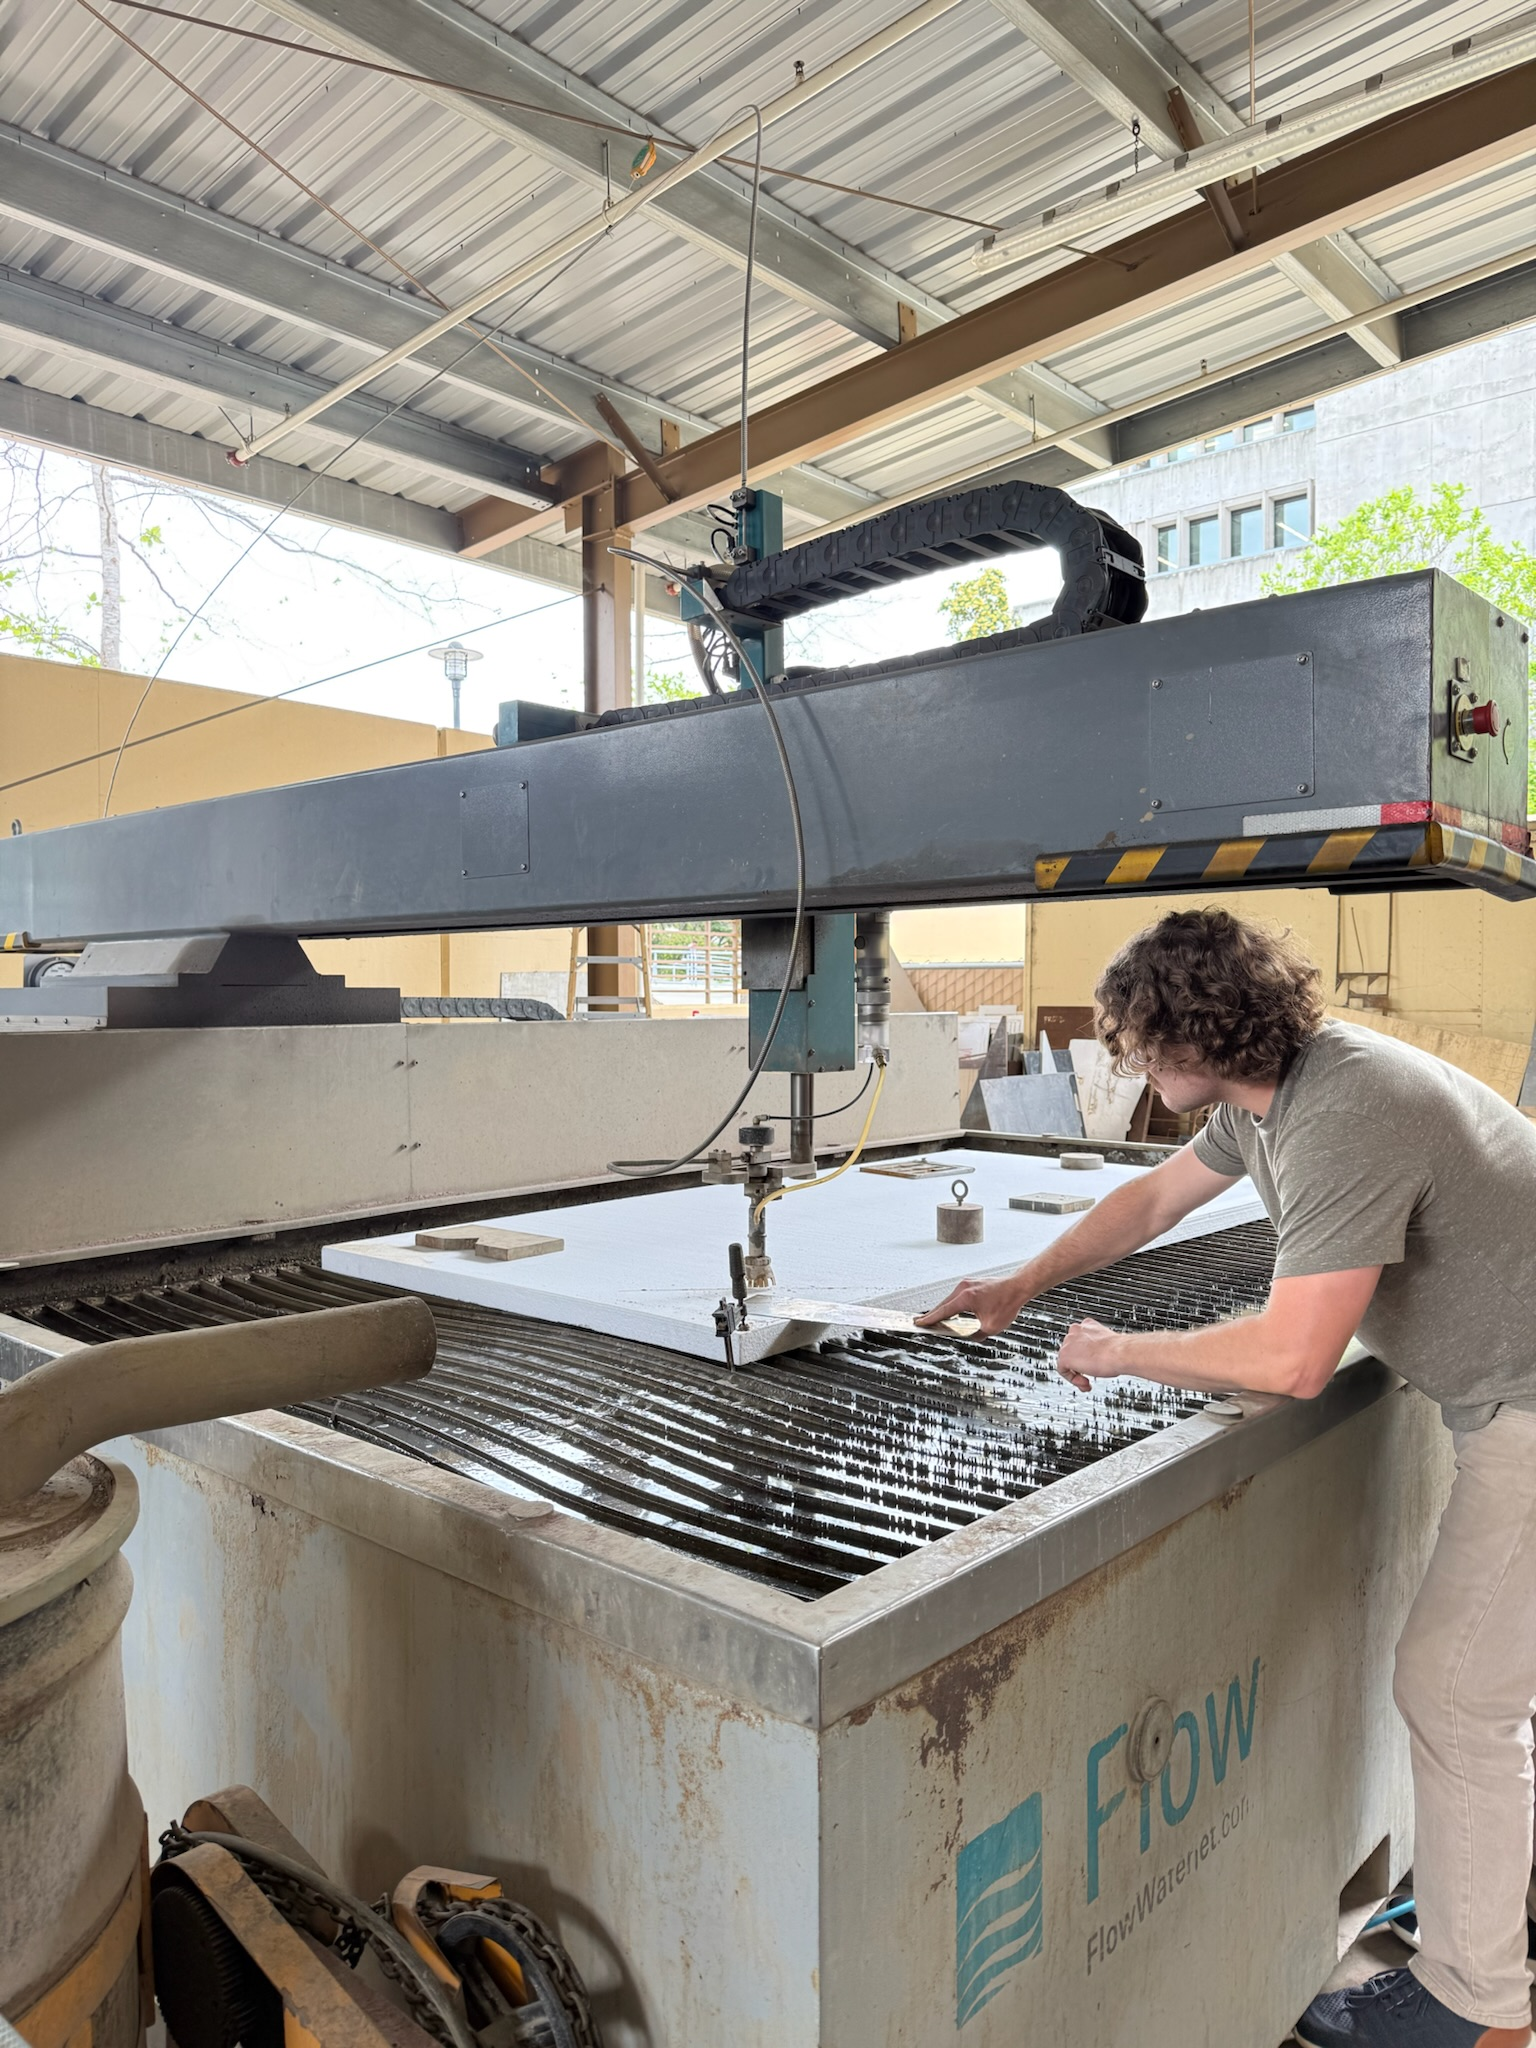
\includegraphics[
        width=3.10in,
        height=1.40in,
        keepaspectratio
    ]{waterjet_foam}
};
\draw[RuleGray,line width=0.55pt,rounded corners=4pt]
    ($(current page.north west)+(0.43in,-3.36in)$)
    rectangle
    ($(current page.north west)+(3.71in,-4.85in)$);

% Row 1 image 2
\node[anchor=center,inner sep=0pt]
at ($(current page.north west)+(5.50in,-4.105in)$)
{
    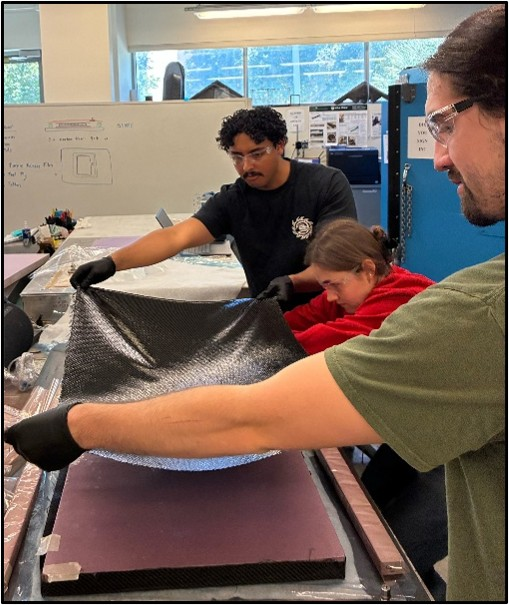
\includegraphics[
        width=3.10in,
        height=1.40in,
        keepaspectratio
    ]{group_layup}
};
\draw[RuleGray,line width=0.55pt,rounded corners=4pt]
    ($(current page.north west)+(3.86in,-3.36in)$)
    rectangle
    ($(current page.north west)+(7.14in,-4.85in)$);

% Row 1 image 3
\node[anchor=center,inner sep=0pt]
at ($(current page.north west)+(8.935in,-4.105in)$)
{
    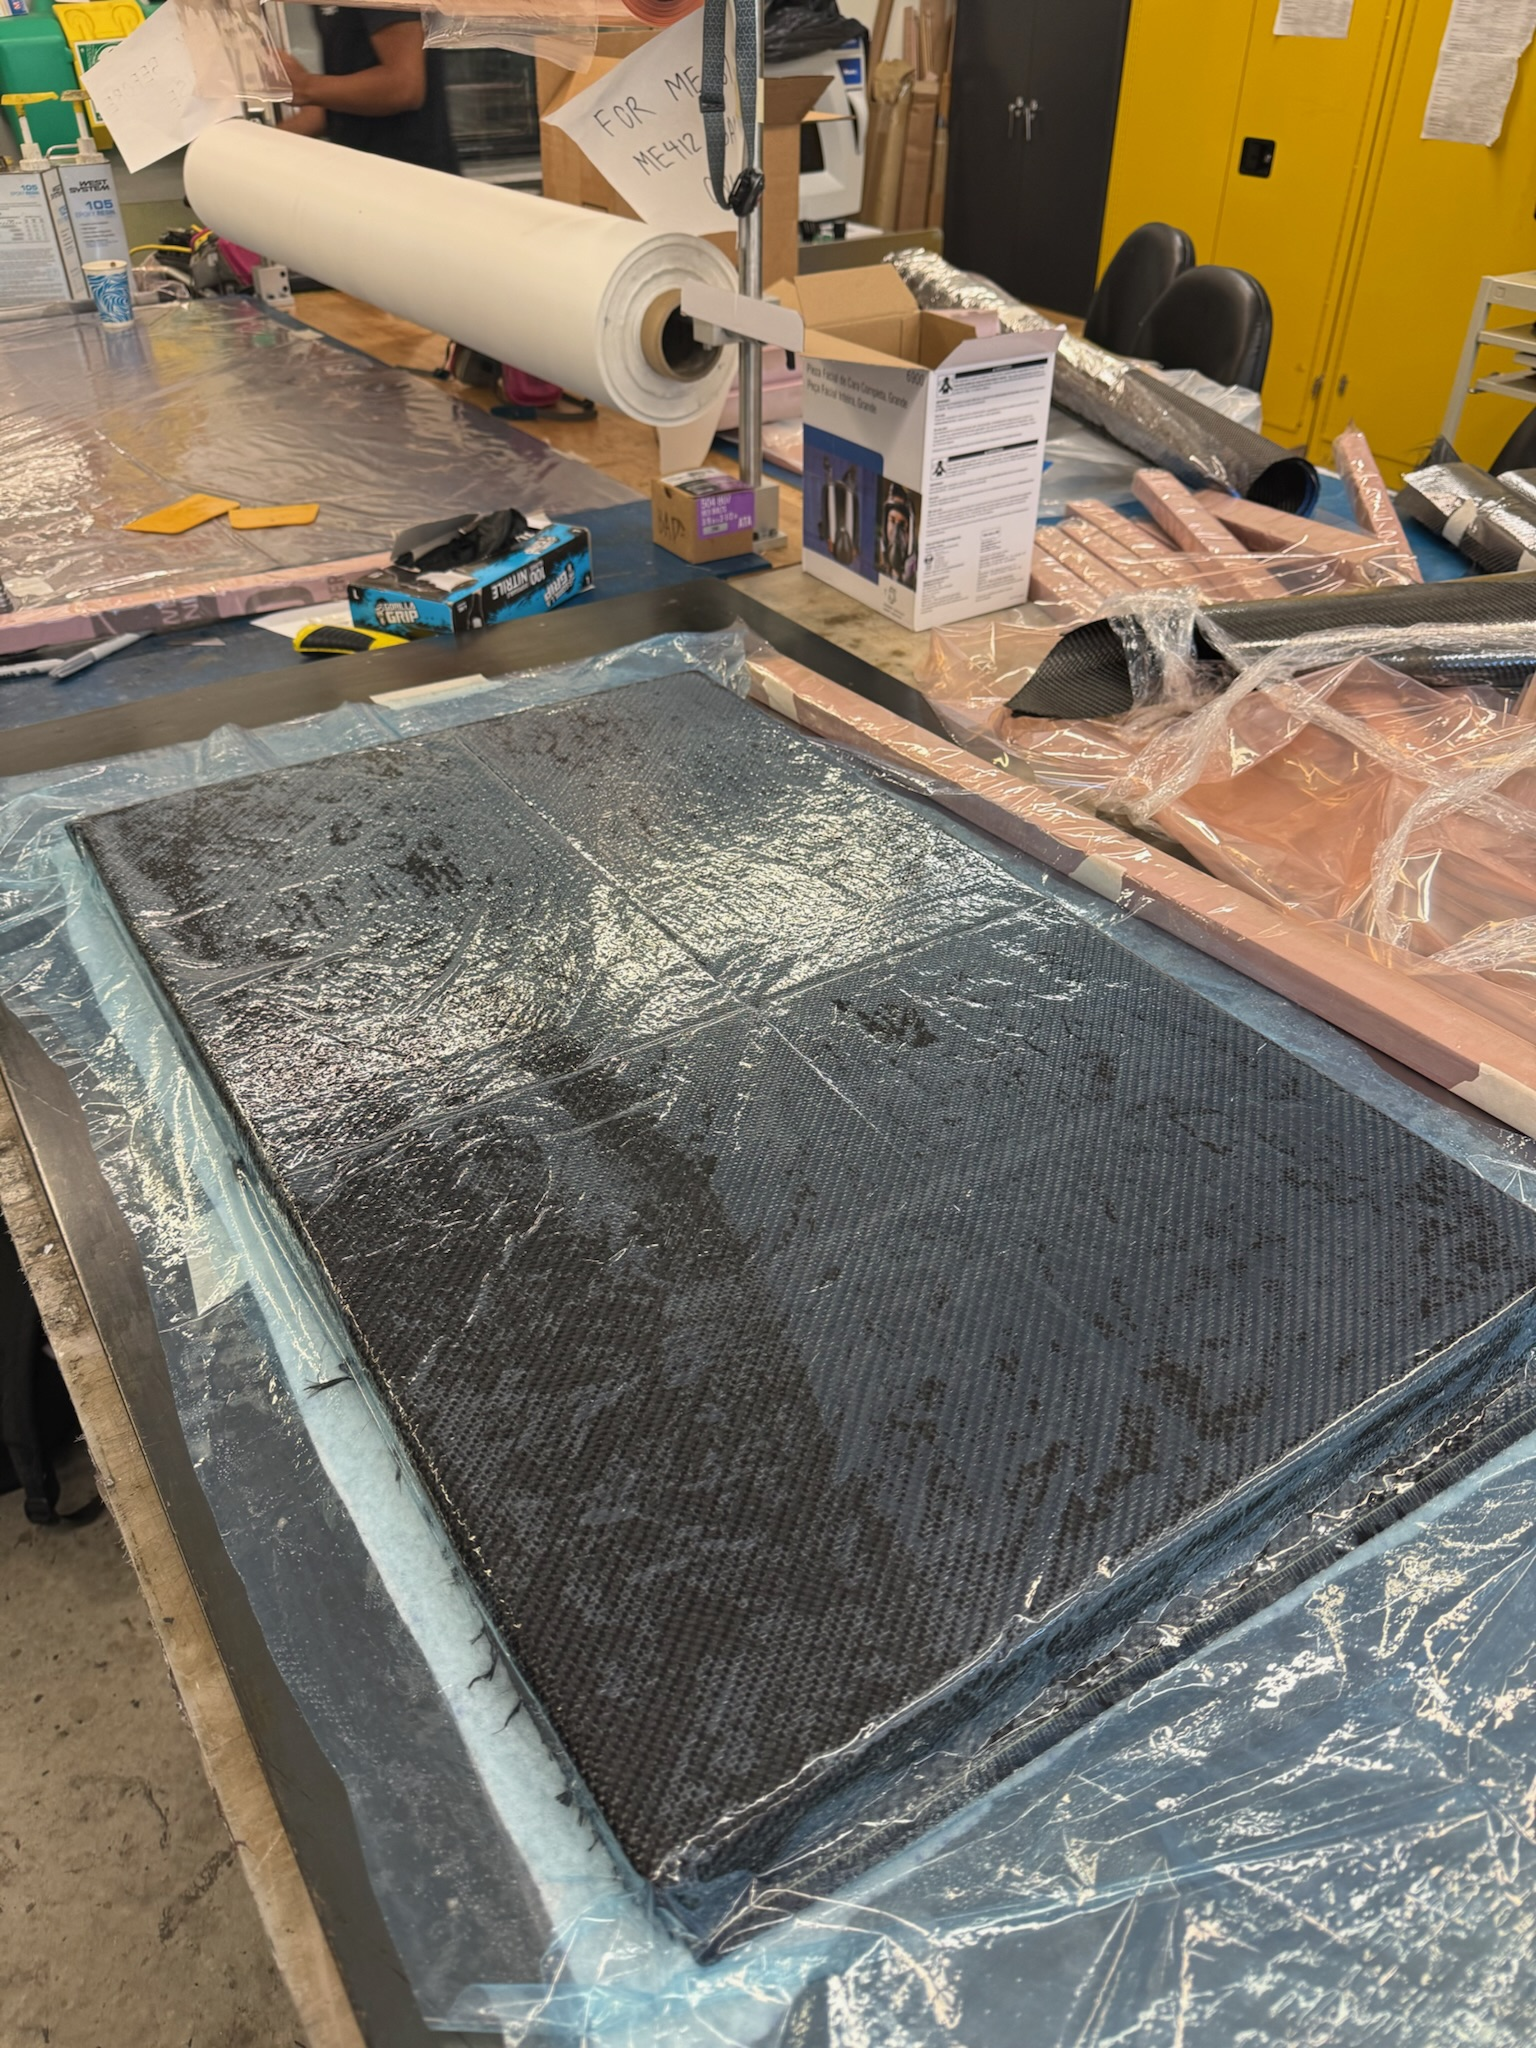
\includegraphics[
        width=3.10in,
        height=1.40in,
        keepaspectratio
    ]{blue_perforrated_film_layup}
};
\draw[RuleGray,line width=0.55pt,rounded corners=4pt]
    ($(current page.north west)+(7.29in,-3.36in)$)
    rectangle
    ($(current page.north east)+(-0.42in,-4.85in)$);

% Row 1 captions
\node[anchor=north,text=Muted,font=\sffamily\fontsize{6.7}{7.3}\selectfont]
at ($(current page.north west)+(2.07in,-4.90in)$)
{1. Waterjet-cut core and perimeter geometry};

\node[anchor=north,text=Muted,font=\sffamily\fontsize{6.7}{7.3}\selectfont]
at ($(current page.north west)+(5.50in,-4.90in)$)
{2. Team wet layup under my process guidance};

\node[anchor=north,text=Muted,font=\sffamily\fontsize{6.7}{7.3}\selectfont]
at ($(current page.north west)+(8.935in,-4.90in)$)
{3. Perforated film, breather, and vacuum enclosure};

% Row 2 image 1
\node[anchor=center,inner sep=0pt]
at ($(current page.north west)+(2.07in,-5.875in)$)
{
    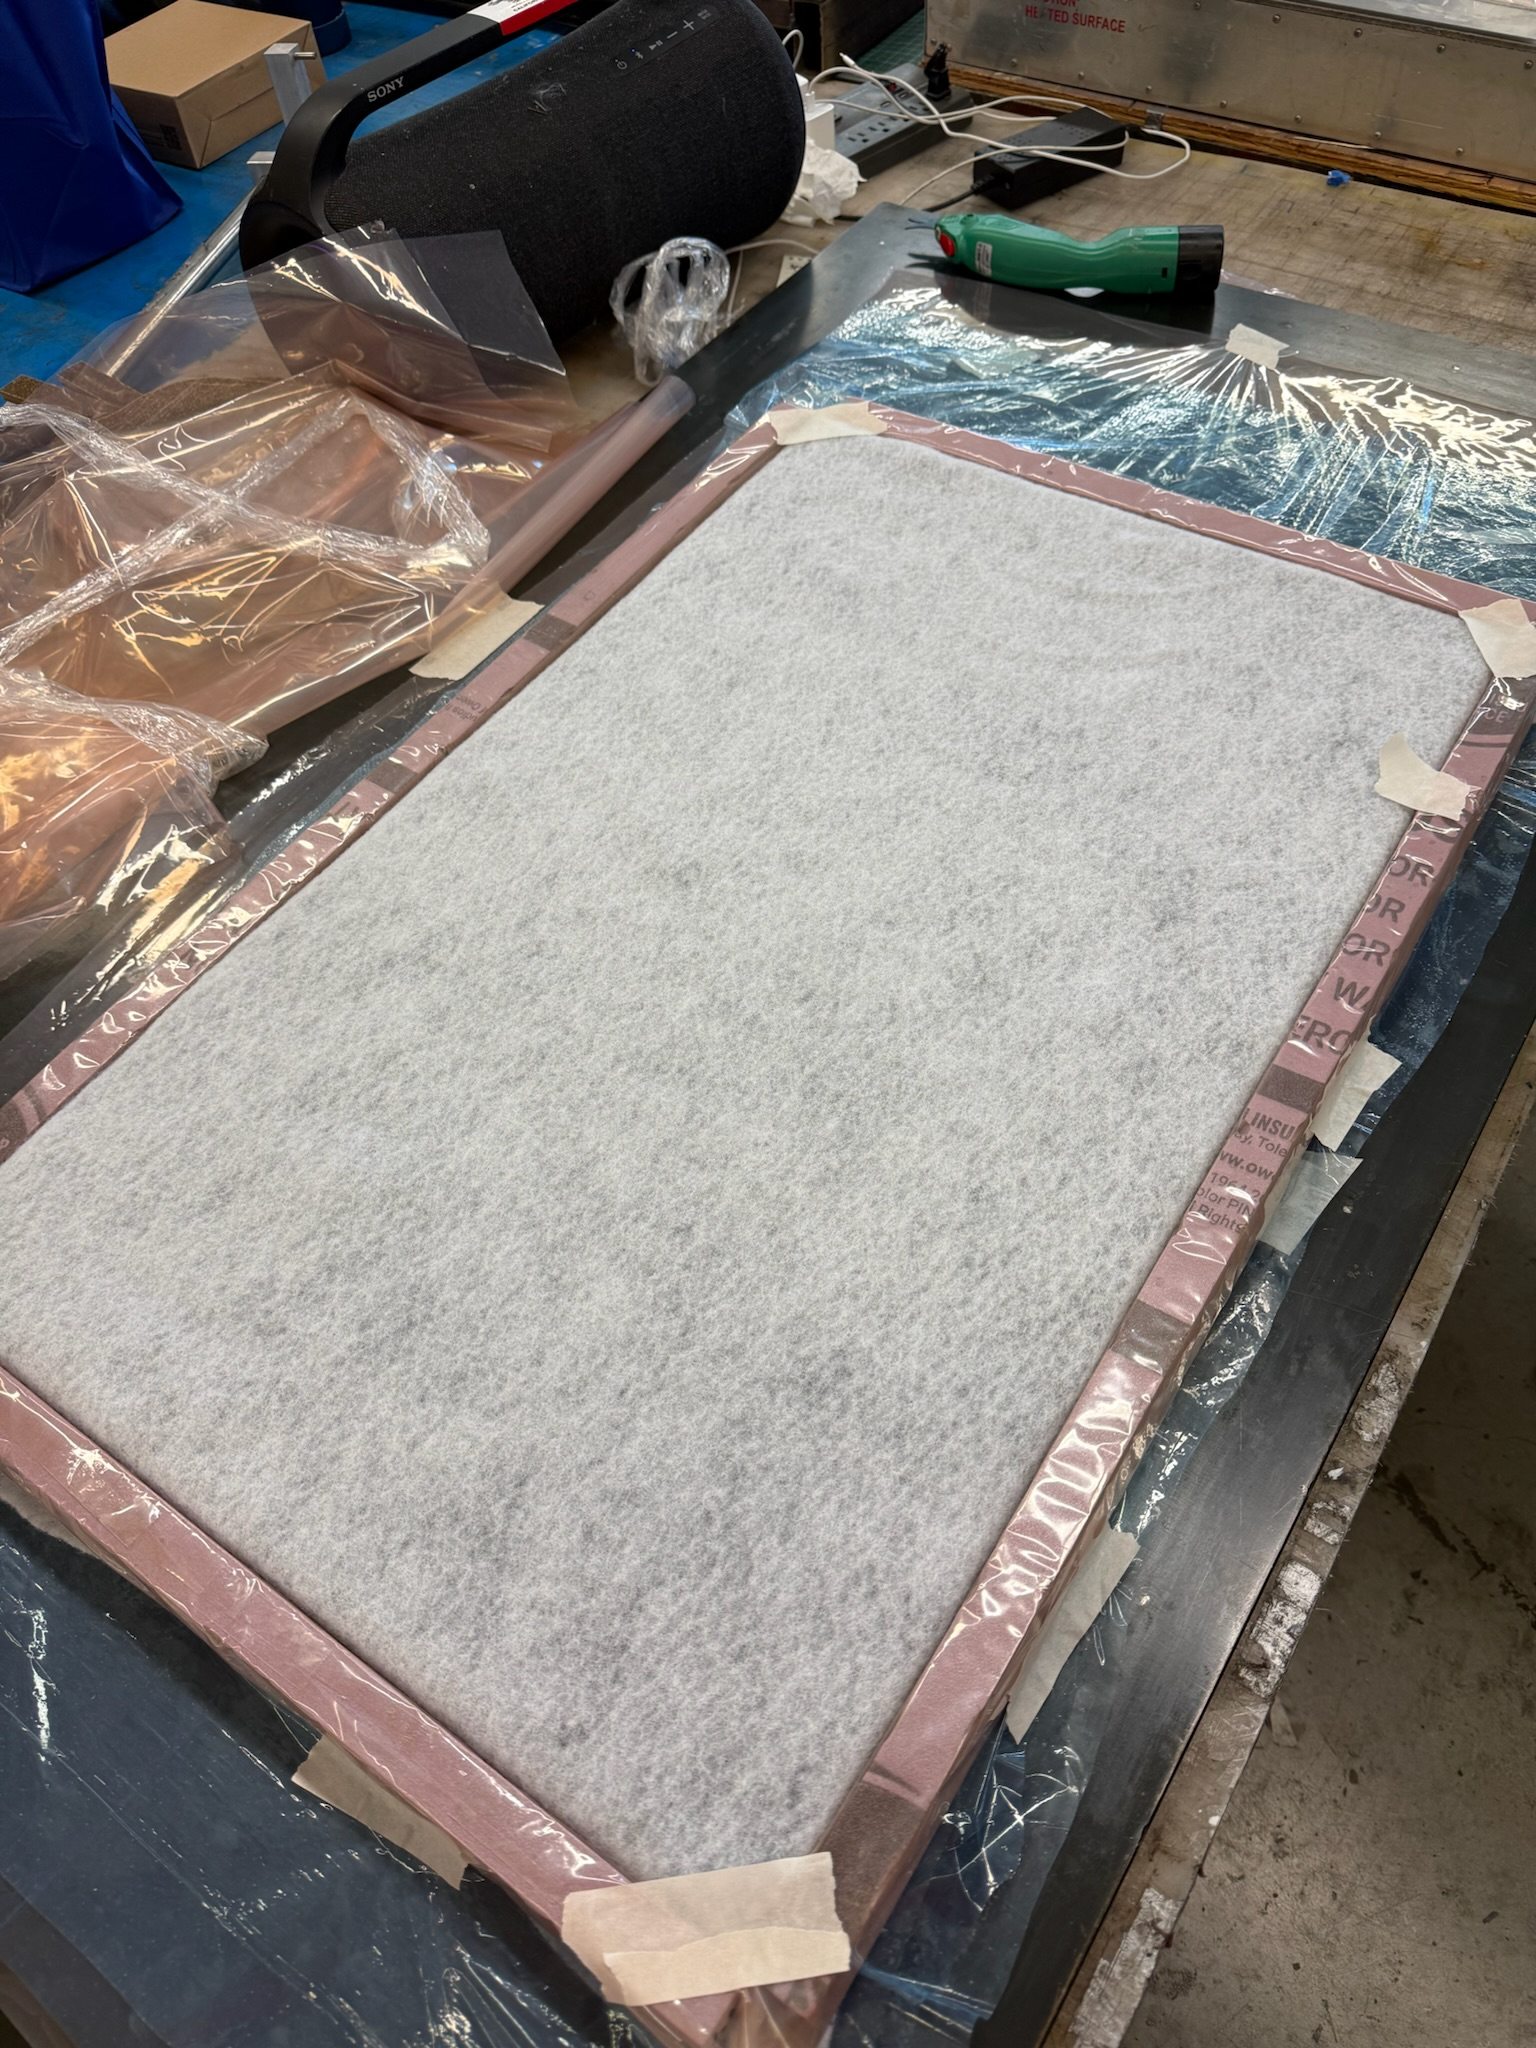
\includegraphics[
        width=3.10in,
        height=1.40in,
        keepaspectratio
    ]{completed_layup}
};
\draw[RuleGray,line width=0.55pt,rounded corners=4pt]
    ($(current page.north west)+(0.43in,-5.13in)$)
    rectangle
    ($(current page.north west)+(3.71in,-6.62in)$);

% Row 2 image 2 — oven chamber used only as a reliable vacuum enclosure; no heat applied
\node[anchor=center,inner sep=0pt]
at ($(current page.north west)+(5.50in,-5.875in)$)
{
    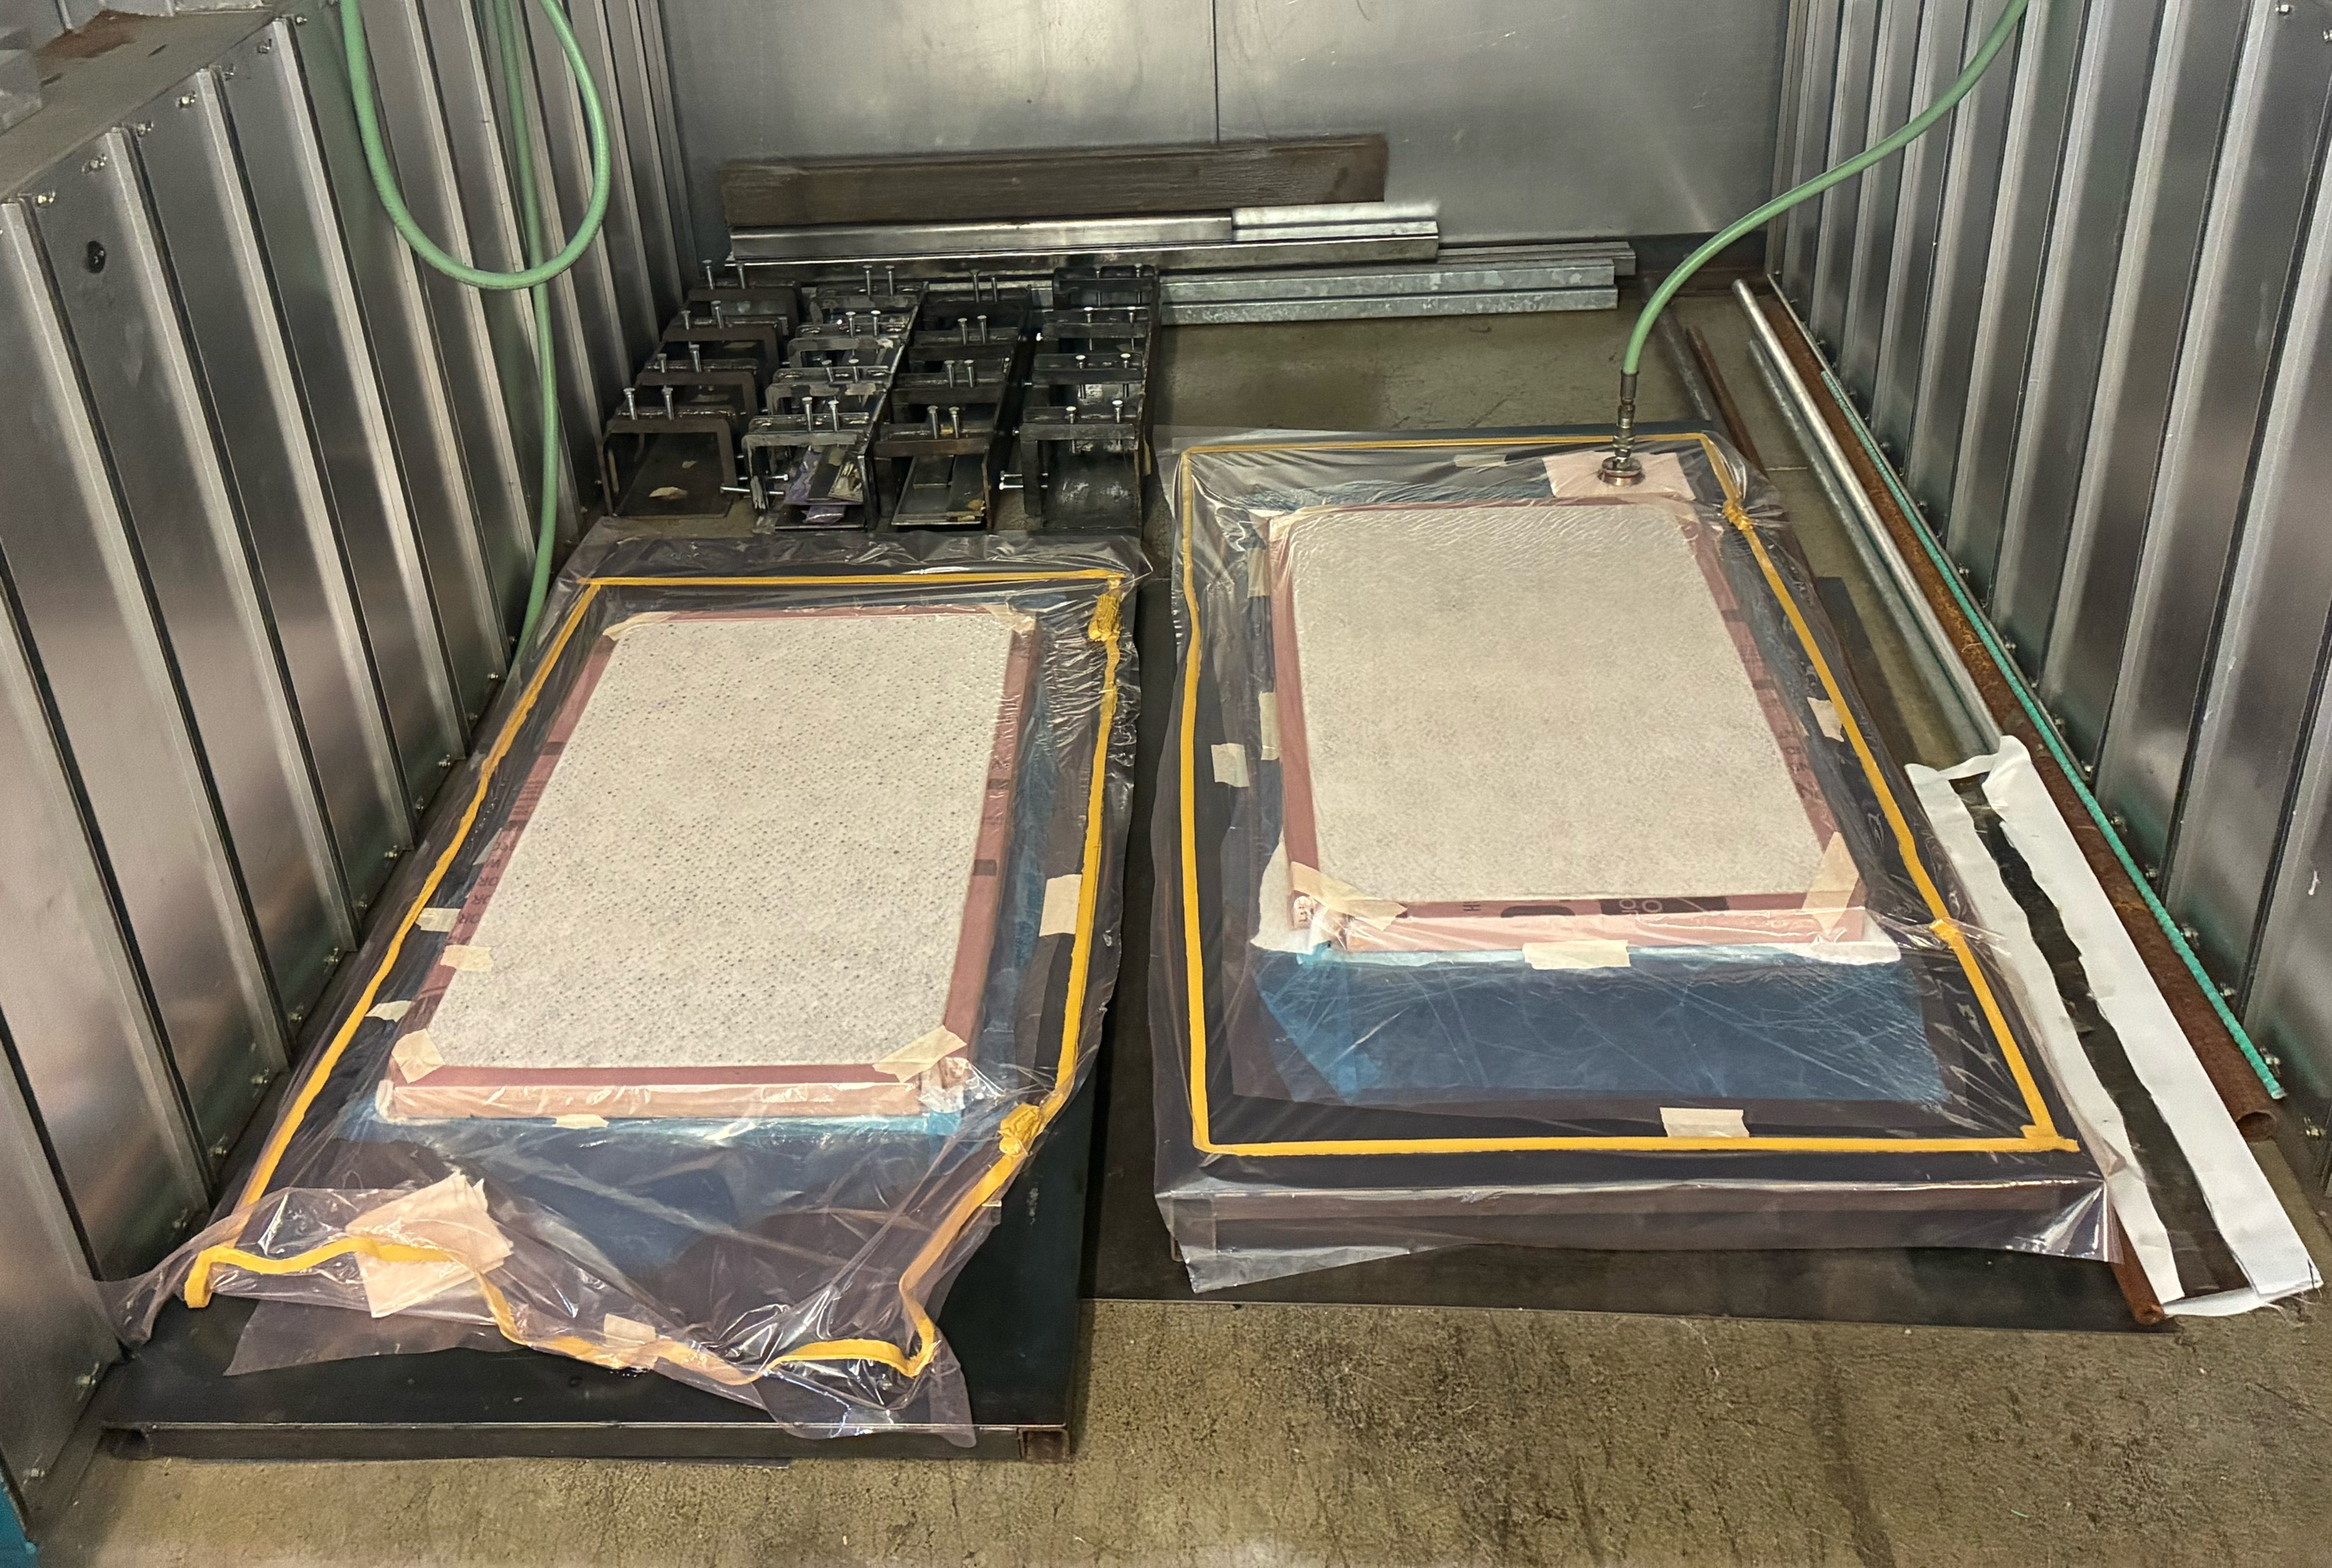
\includegraphics[
        width=3.10in,
        height=1.40in,
        keepaspectratio
    ]{layups_in_composite_oven_under_vacuumPressure}
};
\draw[RuleGray,line width=0.55pt,rounded corners=4pt]
    ($(current page.north west)+(3.86in,-5.13in)$)
    rectangle
    ($(current page.north west)+(7.14in,-6.62in)$);

% Row 2 image 3
\node[anchor=center,inner sep=0pt]
at ($(current page.north west)+(8.935in,-5.875in)$)
{
    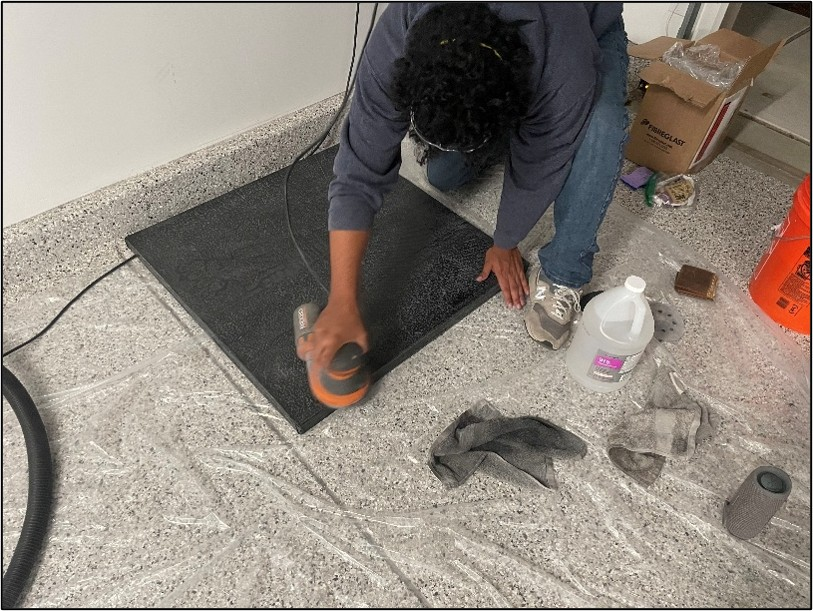
\includegraphics[
        width=3.10in,
        height=1.40in,
        keepaspectratio
    ]{garage_sanding}
};
\draw[RuleGray,line width=0.55pt,rounded corners=4pt]
    ($(current page.north west)+(7.29in,-5.13in)$)
    rectangle
    ($(current page.north east)+(-0.42in,-6.62in)$);

% Row 2 captions
\node[anchor=north,text=Muted,font=\sffamily\fontsize{6.7}{7.3}\selectfont]
at ($(current page.north west)+(2.07in,-6.67in)$)
{4. Fully saturated carbon skin and foam sandwich};

\node[anchor=north,text=Muted,font=\sffamily\fontsize{6.7}{7.3}\selectfont]
at ($(current page.north west)+(5.50in,-6.67in)$)
{5. Room-temperature cure under continuous vacuum};

\node[anchor=north,text=Muted,font=\sffamily\fontsize{6.7}{7.3}\selectfont]
at ($(current page.north west)+(8.935in,-6.67in)$)
{6. Post-processing and surface preparation};

% Bottom callouts
\fill[Panel,rounded corners=4pt]
    ($(current page.north west)+(0.43in,-6.95in)$)
    rectangle
    ($(current page.north west)+(5.48in,-7.60in)$);

\draw[RuleGray,line width=0.55pt,rounded corners=4pt]
    ($(current page.north west)+(0.43in,-6.95in)$)
    rectangle
    ($(current page.north west)+(5.48in,-7.60in)$);

\node[
    anchor=north west,
    text=DeepGreen,
    font=\sffamily\bfseries\fontsize{7.0}{7.6}\selectfont
]
at ($(current page.north west)+(0.63in,-7.08in)$)
{FROM THREE LAYUPS TO ONE};

\node[
    anchor=north west,
    align=left,
    text width=4.56in,
    text=Ink,
    font=\fontsize{6.45}{7.45}\selectfont
]
at ($(current page.north west)+(0.63in,-7.29in)$)
{
The Envelope Method reduced labor, cure cycles, handling,
alignment risk, and time spent forming numerous vacuum-bag
pleats around the 1.5-inch-thick XPS panels.
};

\fill[Panel,rounded corners=4pt]
    ($(current page.north west)+(5.68in,-6.95in)$)
    rectangle
    ($(current page.north east)+(-0.42in,-7.60in)$);

\draw[RuleGray,line width=0.55pt,rounded corners=4pt]
    ($(current page.north west)+(5.68in,-6.95in)$)
    rectangle
    ($(current page.north east)+(-0.42in,-7.60in)$);

\node[
    anchor=north west,
    text=DeepGreen,
    font=\sffamily\bfseries\fontsize{7.0}{7.6}\selectfont
]
at ($(current page.north west)+(5.88in,-7.08in)$)
{WHY SURFACE-BONDED HARDWARE};

\node[
    anchor=north west,
    align=left,
    text width=4.55in,
    text=Ink,
    font=\fontsize{6.45}{7.45}\selectfont
]
at ($(current page.north west)+(5.88in,-7.29in)$)
{
Adhesively bonded hinges and fixtures preserved the clean
composite exterior and avoided drilled inserts, foam-core
crushing, added stress concentrations, and new leak paths.
};


% Footer
\node[
    anchor=south west,
    text=white,
    font=\sffamily\bfseries\fontsize{7.1}{7.7}\selectfont
]
at ($(current page.south west)+(0.42in,0.17in)$)
{\faArrowLeft\ PRODUCT ARCHITECTURE};

\node[
    anchor=south,
    text=white,
    font=\sffamily\fontsize{7.0}{7.6}\selectfont
]
at ($(current page.south)+(0,0.17in)$)
{TORO COVER \hspace{6pt} 2 / 3};

\node[
    anchor=south east,
    text=white,
    font=\sffamily\bfseries\fontsize{7.1}{7.7}\selectfont
]
at ($(current page.south east)+(-0.42in,0.17in)$)
{VALIDATION \& TAKEAWAYS \faArrowRight};

\end{tikzpicture}


% ============================================================
% PAGE 3 — FINISHING, VALIDATION, AND TAKEAWAYS
% ============================================================

\clearpage
\thispagestyle{empty}
\hypertarget{toro-results}{}
\null

\begin{tikzpicture}[remember picture,overlay]

% Background and bars
\fill[white]
    (current page.south west)
    rectangle
    (current page.north east);

\fill[DeepGreen]
    (current page.north west)
    rectangle
    ($(current page.north east)+(0,-0.095in)$);

\fill[PolyGold]
    ($(current page.north west)+(0,-0.095in)$)
    rectangle
    ($(current page.north east)+(0,-0.14in)$);

\fill[DeepGreen]
    (current page.south west)
    rectangle
    ($(current page.south east)+(0,0.36in)$);

\fill[PolyGold]
    ($(current page.south west)+(0,0.36in)$)
    rectangle
    ($(current page.south east)+(0,0.405in)$);

% Header
\node[
    anchor=north west,
    text=PolyGold,
    font=\sffamily\bfseries\fontsize{8.1}{8.7}\selectfont
]
at ($(current page.north west)+(0.42in,-0.39in)$)
{TORO COVER \hspace{5pt}/\hspace{5pt} VALIDATION AND ENGINEERING TAKEAWAYS};

\node[
    anchor=north west,
    text=DeepGreen,
    font=\bfseries\fontsize{22.5}{23.5}\selectfont
]
at ($(current page.north west)+(0.40in,-0.67in)$)
{FROM PROTOTYPE TO PRODUCT PATHWAY};

\node[
    anchor=north west,
    text=Muted,
    font=\sffamily\fontsize{8.7}{9.6}\selectfont
]
at ($(current page.north west)+(0.42in,-1.12in)$)
{Environmental protection, usability testing, scope decisions, and lessons from technical leadership};

\fill[PolyGold]
    ($(current page.north west)+(0.42in,-1.36in)$)
    rectangle
    ($(current page.north west)+(5.8in,-1.315in)$);

% Finishing title
\node[
    anchor=north west,
    text=DeepGreen,
    font=\sffamily\bfseries\fontsize{8.0}{8.7}\selectfont
]
at ($(current page.north west)+(0.43in,-1.62in)$)
{OUTDOOR FINISHING AND ENVIRONMENTAL PROTECTION};

% Image 1
\node[anchor=center,inner sep=0pt]
at ($(current page.north west)+(1.705in,-2.655in)$)
{
    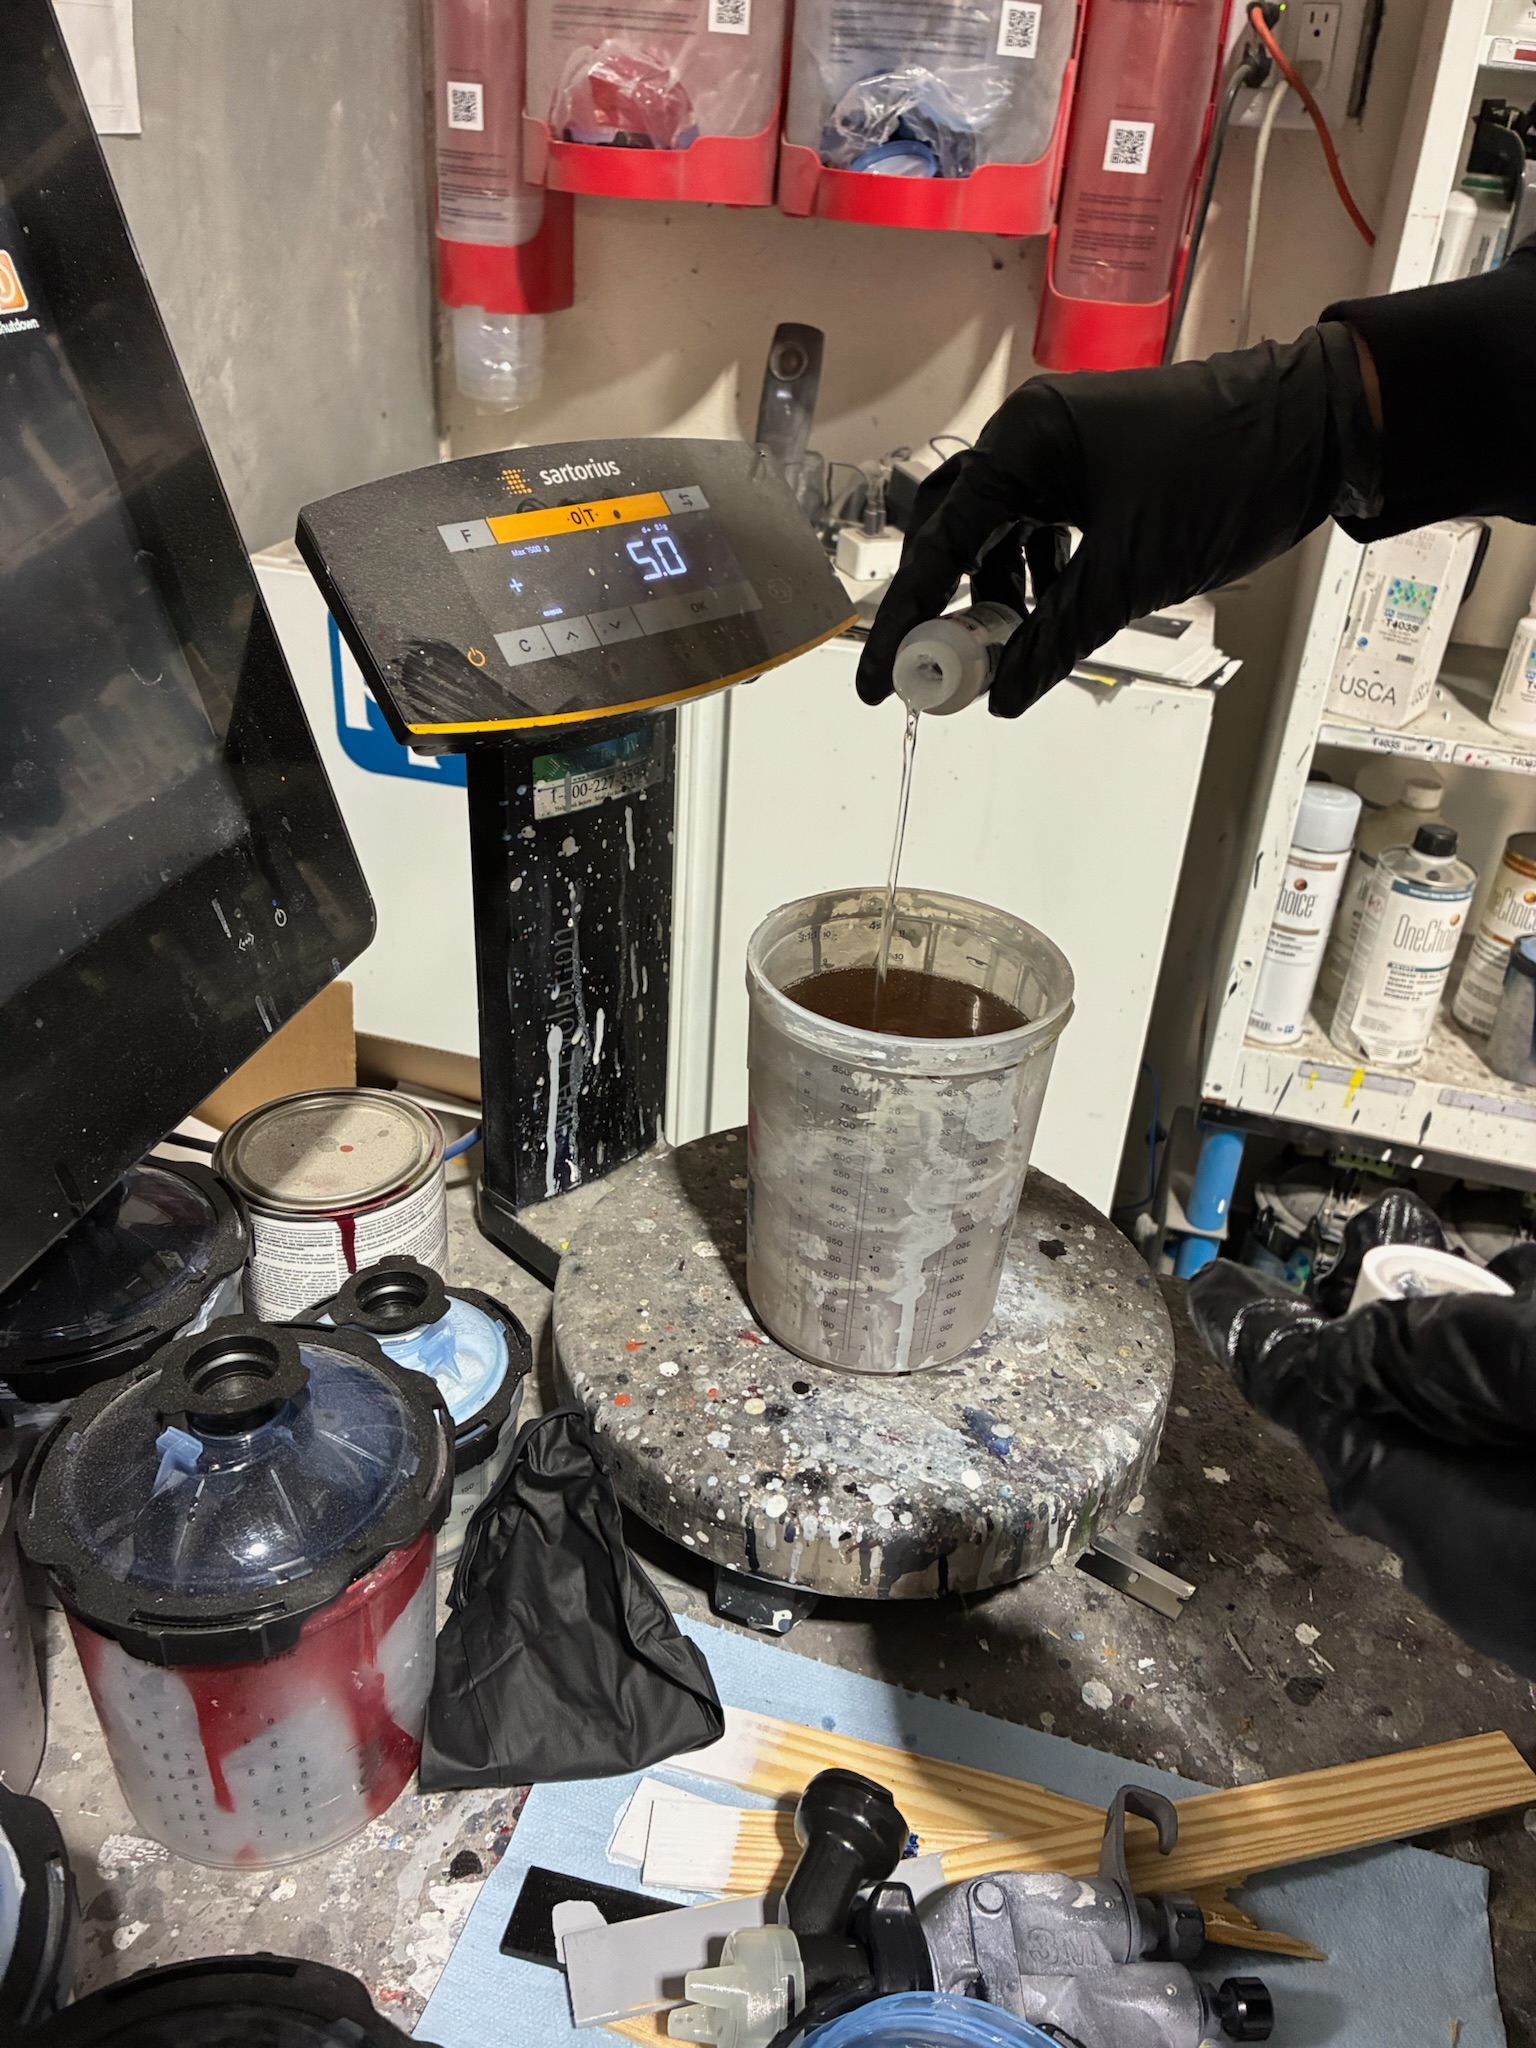
\includegraphics[
        width=2.35in,
        height=1.40in,
        keepaspectratio
    ]{spray_topcoat_prep}
};
\draw[RuleGray,line width=0.55pt,rounded corners=4pt]
    ($(current page.north west)+(0.43in,-1.91in)$)
    rectangle
    ($(current page.north west)+(2.98in,-3.40in)$);

% Image 2
\node[anchor=center,inner sep=0pt]
at ($(current page.north west)+(4.375in,-2.655in)$)
{
    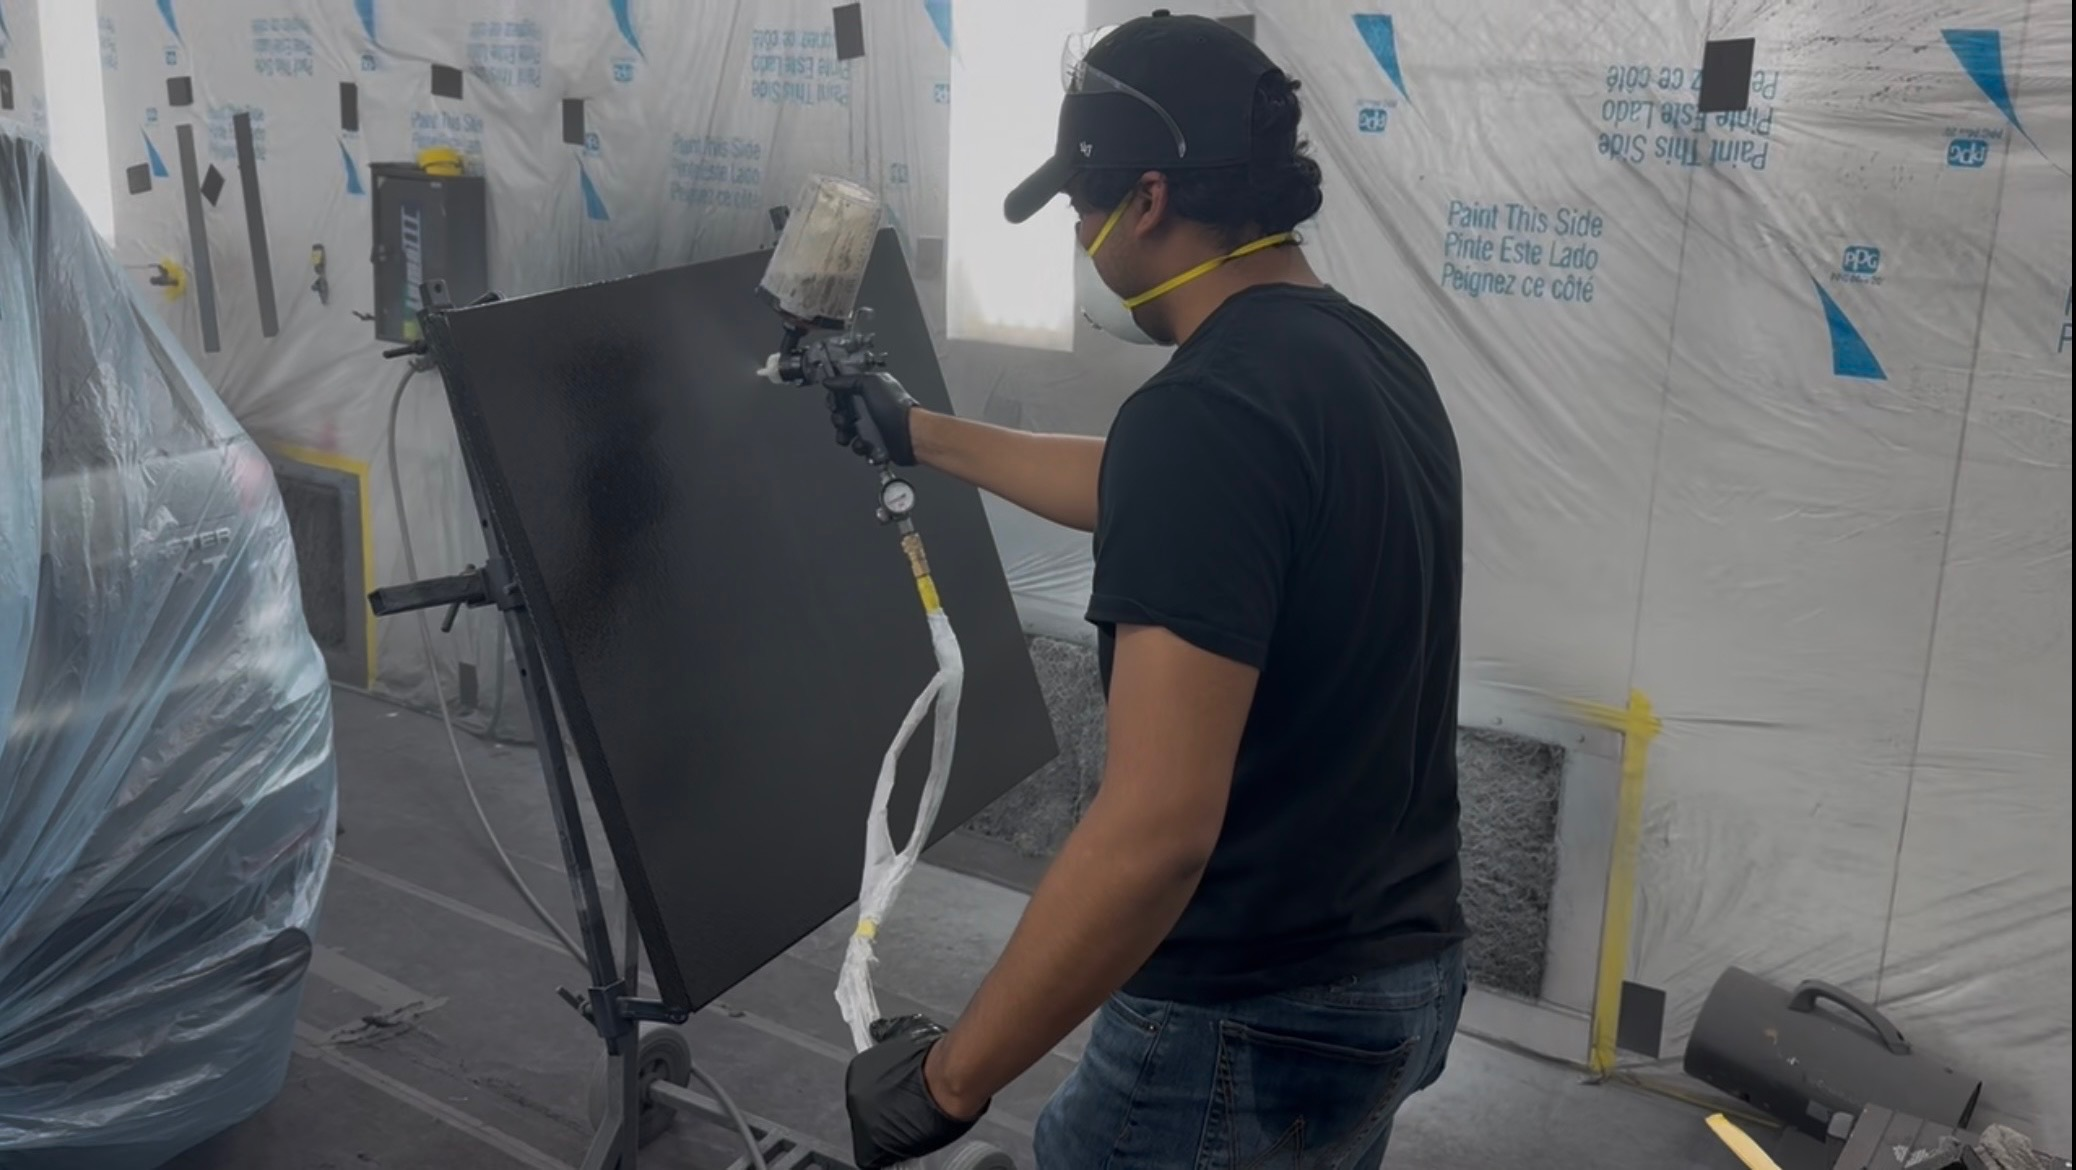
\includegraphics[
        width=2.35in,
        height=1.40in,
        keepaspectratio
    ]{spraying_topcoat}
};
\draw[RuleGray,line width=0.55pt,rounded corners=4pt]
    ($(current page.north west)+(3.10in,-1.91in)$)
    rectangle
    ($(current page.north west)+(5.65in,-3.40in)$);

% Image 3
\node[anchor=center,inner sep=0pt]
at ($(current page.north west)+(7.045in,-2.655in)$)
{
    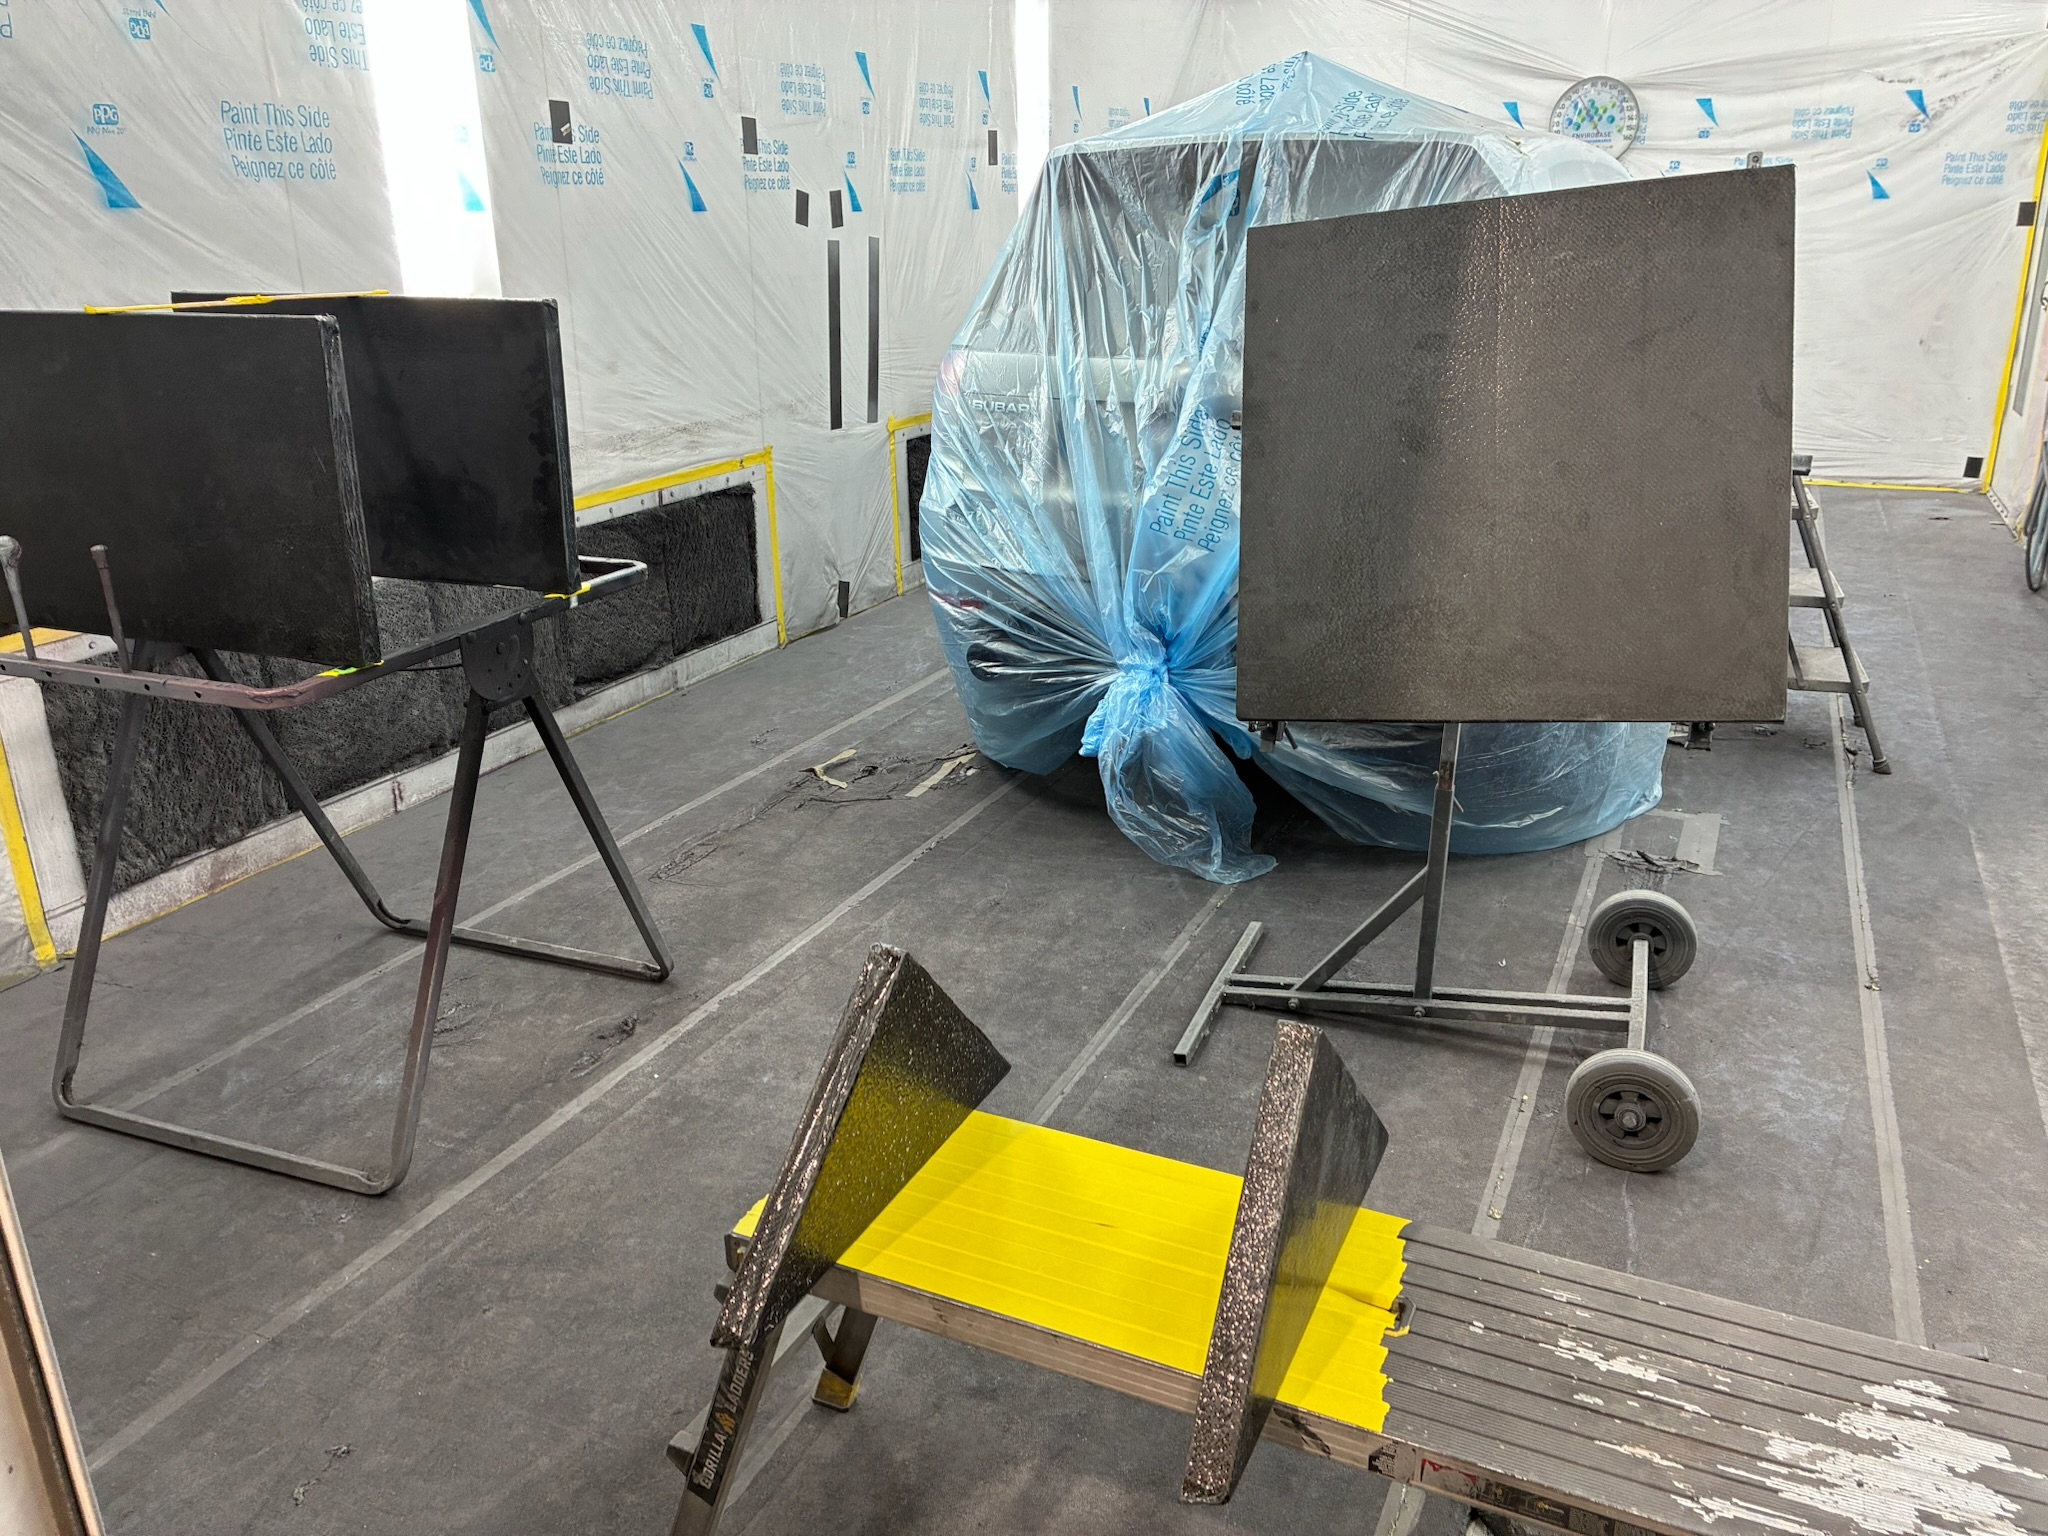
\includegraphics[
        width=2.35in,
        height=1.40in,
        keepaspectratio
    ]{topcoat_setup_apparatus}
};
\draw[RuleGray,line width=0.55pt,rounded corners=4pt]
    ($(current page.north west)+(5.77in,-1.91in)$)
    rectangle
    ($(current page.north west)+(8.32in,-3.40in)$);

% Image 4
\node[anchor=center,inner sep=0pt]
at ($(current page.north west)+(9.50in,-2.655in)$)
{
    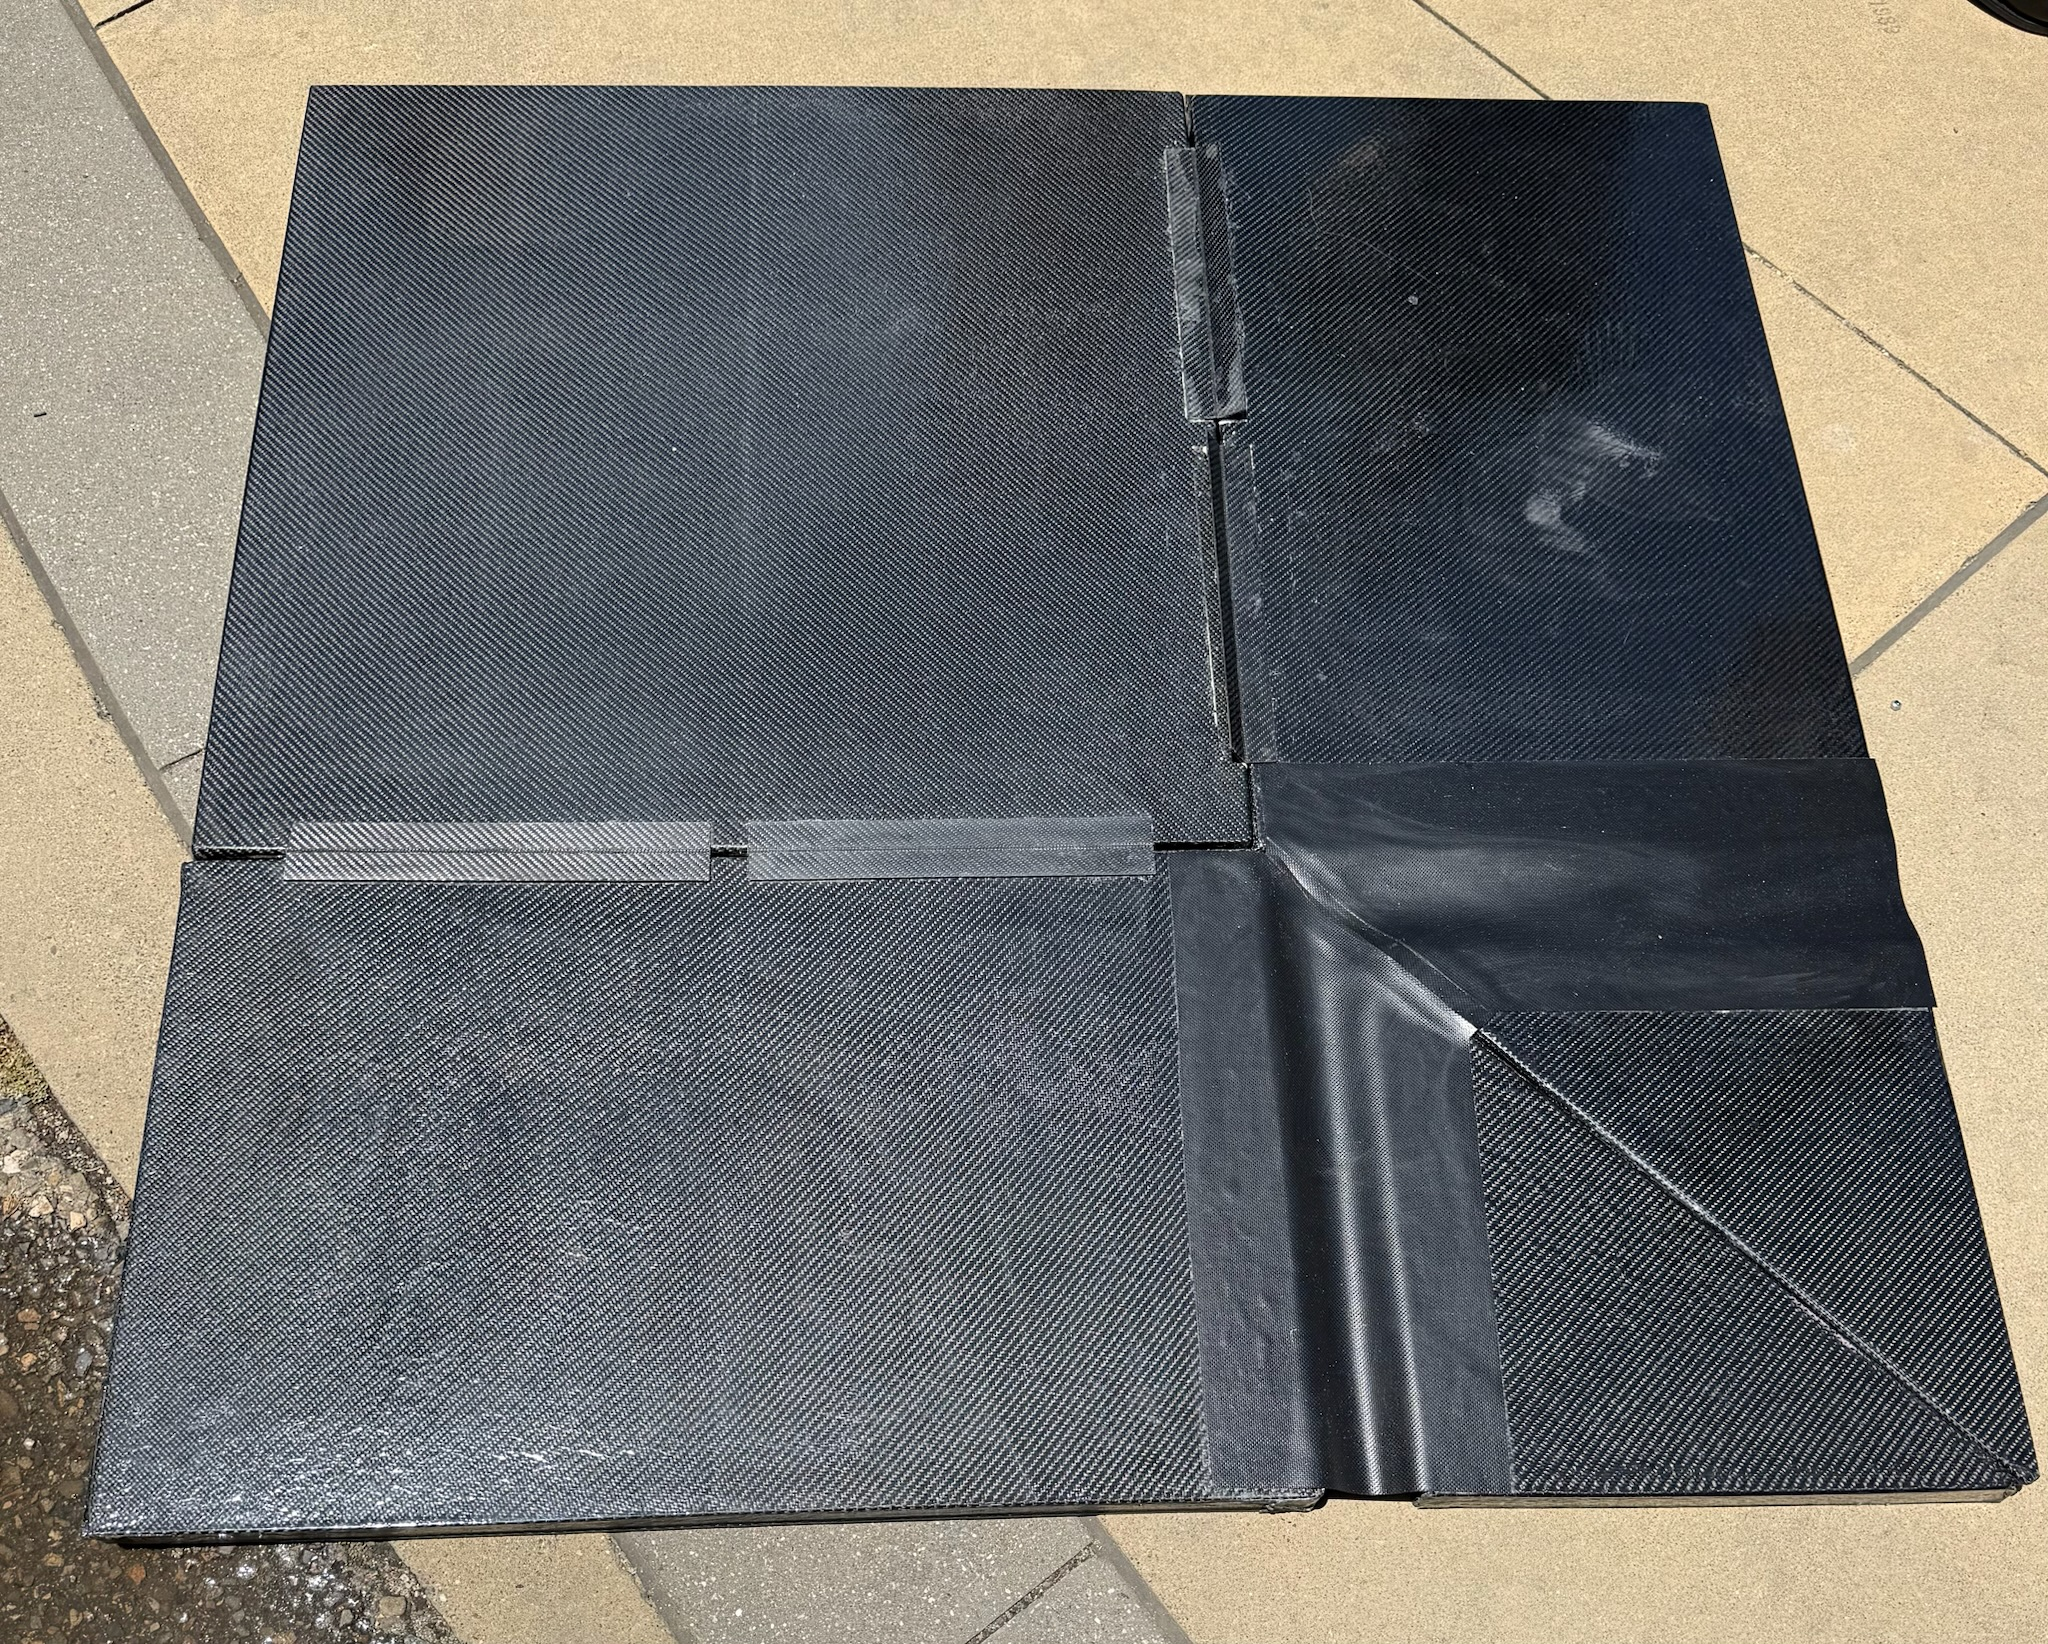
\includegraphics[
        width=2.35in,
        height=1.40in,
        keepaspectratio
    ]{refined_final_toro_cover_partial_carbon_model}
};
\draw[RuleGray,line width=0.55pt,rounded corners=4pt]
    ($(current page.north west)+(8.44in,-1.91in)$)
    rectangle
    ($(current page.north east)+(-0.42in,-3.40in)$);

% Captions
\node[anchor=north,text=Muted,font=\sffamily\fontsize{6.7}{7.3}\selectfont]
at ($(current page.north west)+(1.705in,-3.45in)$)
{Topcoat material preparation};

\node[anchor=north,text=Muted,font=\sffamily\fontsize{6.7}{7.3}\selectfont]
at ($(current page.north west)+(4.375in,-3.45in)$)
{Automotive-booth topcoat application};

\node[anchor=north,text=Muted,font=\sffamily\fontsize{6.7}{7.3}\selectfont]
at ($(current page.north west)+(7.045in,-3.45in)$)
{Coated panels drying after application};

\node[anchor=north,text=Muted,font=\sffamily\fontsize{6.7}{7.3}\selectfont]
at ($(current page.north west)+(9.50in,-3.45in)$)
{Partial carbon manufacturing model};

% Environmental rationale
\fill[SoftGold,rounded corners=4pt]
    ($(current page.north west)+(0.43in,-3.73in)$)
    rectangle
    ($(current page.north east)+(-0.42in,-4.76in)$);

\node[
    anchor=north west,
    align=left,
    text width=9.75in,
    text=Ink,
    font=\fontsize{7.05}{8.25}\selectfont
]
at ($(current page.north west)+(0.65in,-3.89in)$)
{
Because the sponsor required a carbon-fiber cover for outdoor use near chlorinated water,
environmental protection became a functional requirement rather than a cosmetic finish.
I selected and personally sprayed a UV-resistant Sunshield topcoat to seal minor laminate
porosity, reduce moisture ingress, preserve the carbon appearance, limit UV degradation of
the epoxy matrix, and isolate the composite surface from nearby metallic hardware.
};

% Results title
\node[
    anchor=north west,
    text=DeepGreen,
    font=\sffamily\bfseries\fontsize{8.0}{8.7}\selectfont
]
at ($(current page.north west)+(0.43in,-4.94in)$)
{FUNCTIONAL PROTOTYPE RESULTS};

% ------------------------------------------------------------
% Matched lower panels — larger type and improved allocation
% ------------------------------------------------------------

% Left results panel
\fill[SoftGreen,rounded corners=5pt]
    ($(current page.north west)+(0.43in,-5.22in)$)
    rectangle
    ($(current page.north west)+(5.98in,-7.39in)$);

\draw[RuleGray,line width=0.65pt,rounded corners=5pt]
    ($(current page.north west)+(0.43in,-5.22in)$)
    rectangle
    ($(current page.north west)+(5.98in,-7.39in)$);

\fill[DeepGreen,rounded corners=5pt]
    ($(current page.north west)+(0.43in,-5.22in)$)
    rectangle
    ($(current page.north west)+(5.98in,-5.58in)$);

\fill[DeepGreen]
    ($(current page.north west)+(0.43in,-5.40in)$)
    rectangle
    ($(current page.north west)+(5.98in,-5.58in)$);

\node[anchor=west,text=white,
      font=\sffamily\bfseries\fontsize{7.0}{7.6}\selectfont]
at ($(current page.north west)+(0.66in,-5.40in)$)
{SPECIFICATION};

\node[anchor=west,text=white,
      font=\sffamily\bfseries\fontsize{7.0}{7.6}\selectfont]
at ($(current page.north west)+(3.02in,-5.40in)$)
{RESULT};

\node[anchor=east,text=white,
      font=\sffamily\bfseries\fontsize{7.0}{7.6}\selectfont]
at ($(current page.north west)+(5.55in,-5.40in)$)
{STATUS};

\node[
    anchor=north west,
    align=left,
    text width=2.15in,
    text=Ink,
    font=\bfseries\fontsize{7.15}{8.55}\selectfont
]
at ($(current page.north west)+(0.66in,-5.72in)$)
{
Deployment time\\[3.4pt]
Removal time\\[3.4pt]
Single-user operation\\[3.4pt]
Single-side operation\\[3.4pt]
Deployment steps\\[3.4pt]
Removal steps\\[3.4pt]
Weight\\[3.4pt]
Folded storage
};

\node[
    anchor=north west,
    align=left,
    text width=1.45in,
    text=Ink,
    font=\fontsize{7.15}{8.55}\selectfont
]
at ($(current page.north west)+(3.02in,-5.72in)$)
{
25.51 seconds\\[3.4pt]
37.22 seconds\\[3.4pt]
100\% successful\\[3.4pt]
75\% successful\\[3.4pt]
6.4 average\\[3.4pt]
9 average\\[3.4pt]
17 lb\\[3.4pt]
2.9' x 2.9' x 1.7'
};

\node[
    anchor=north east,
    align=right,
    text width=1.05in,
    text=DeepGreen,
    font=\sffamily\bfseries\fontsize{7.05}{8.55}\selectfont
]
at ($(current page.north west)+(5.55in,-5.72in)$)
{
PASS\\[3.4pt]
PASS\\[3.4pt]
PASS\\[3.4pt]
NEAR TARGET\\[3.4pt]
PASS\\[3.4pt]
PASS\\[3.4pt]
NEAR TARGET\\[3.4pt]
PASS
};

% Right takeaways panel — widened for easier reading
\fill[SoftGreen,rounded corners=5pt]
    ($(current page.north west)+(6.14in,-5.22in)$)
    rectangle
    ($(current page.north east)+(-0.42in,-7.39in)$);

\draw[RuleGray,line width=0.65pt,rounded corners=5pt]
    ($(current page.north west)+(6.14in,-5.22in)$)
    rectangle
    ($(current page.north east)+(-0.42in,-7.39in)$);

\fill[DeepGreen,rounded corners=5pt]
    ($(current page.north west)+(6.14in,-5.22in)$)
    rectangle
    ($(current page.north east)+(-0.42in,-5.58in)$);

\fill[DeepGreen]
    ($(current page.north west)+(6.14in,-5.40in)$)
    rectangle
    ($(current page.north east)+(-0.42in,-5.58in)$);

\node[anchor=west,text=white,
      font=\sffamily\bfseries\fontsize{7.1}{7.7}\selectfont]
at ($(current page.north west)+(6.38in,-5.40in)$)
{ENGINEERING TAKEAWAYS};

\node[
    anchor=north west,
    align=left,
    text width=4.02in,
    text=Ink,
    font=\fontsize{6.75}{7.85}\selectfont
]
at ($(current page.north west)+(6.38in,-5.72in)$)
{
\textbf{Manufacturing first.}
Composite manufacturing constraints should guide the product architecture from the beginning.\\[4.5pt]
\textbf{Prioritize deliberately.}
Competing requirements must be balanced intentionally instead of maximizing every objective.\\[4.5pt]
\textbf{Lead through the process.}
Clear procedures, calm communication, and respect for teammates' strengths were essential during fabrication.\\[4.5pt]
\textbf{Next iteration.}
Reduce weight, refine the fabric-hinge fold lines, and improve panel-edge clearance.
};

% Compact concluding pathway
\node[
    anchor=center,
    align=center,
    text=PolyGold,
    font=\sffamily\bfseries\fontsize{6.3}{6.9}\selectfont
]
at ($(current page.north)+(3.06in,-7.18in)$)
{PROTOTYPE \faArrowRight\ DESIGN REFINEMENT
\faArrowRight\ REPEATABLE MANUFACTURING
\faArrowRight\ PRODUCT};

% Validation resources
\node[
    anchor=north,
    align=center,
    text=DeepGreen,
    font=\sffamily\bfseries\fontsize{6.6}{7.2}\selectfont
]
at ($(current page.north)+(0,-7.58in)$)
{\href{\ToroDeploymentLink}{\faPlayCircle\ DEPLOYMENT}
\hspace{18pt}
\href{\ToroRemovalLink}{\faPlayCircle\ REMOVAL / FOLDING}
\hspace{18pt}
\href{\ToroPosterLink}{\faFilePdf\ EXPO POSTER}
\hspace{18pt}
\href{\ToroReportLink}{\faFilePdf\ FINAL REPORT}};

% Footer
\node[
    anchor=south west,
    text=white,
    font=\sffamily\bfseries\fontsize{7.1}{7.7}\selectfont
]
at ($(current page.south west)+(0.42in,0.17in)$)
{\faArrowLeft\ MANUFACTURING-DRIVEN DESIGN};

\node[
    anchor=south,
    text=white,
    font=\sffamily\fontsize{7.0}{7.6}\selectfont
]
at ($(current page.south)+(0,0.17in)$)
{TORO COVER \hspace{6pt} 3 / 3};

\node[
    anchor=south east,
    text=white,
    font=\sffamily\bfseries\fontsize{7.1}{7.7}\selectfont
]
at ($(current page.south east)+(-0.42in,0.17in)$)
{NEXT PROJECT \faArrowRight};

\end{tikzpicture}

% ============================================================
% PICKLEBALL PADDLE — SINGLE-PAGE PORTFOLIO CASE STUDY
% Project 02 in the Composites section
%
% IMPORTANT:
% 1. This file must NOT contain \documentclass, \begin{document},
%    or \end{document}.
% 2. In main.tex, place \input{pickleball} before \end{document}.
% 3. Image references use these Overleaf base filenames:
%       waterjet
%       side_core_view
%       full_assy
%       front_view
%       LAMINATE
% ============================================================

% Clickable project resource
\providecommand{\PaddleWaterjetVideo}
{https://drive.google.com/file/d/1mTuaE_g5mE2f7Nn3R5k7yFxqCWH_pvBh/view?usp=drive_link}

\clearpage
\thispagestyle{empty}
\hypertarget{pickleball}{}
\null

\begin{tikzpicture}[remember picture,overlay]

% ============================================================
% BACKGROUND AND PAGE BARS
% ============================================================

\fill[white]
    (current page.south west)
    rectangle
    (current page.north east);

\fill[DeepGreen]
    (current page.north west)
    rectangle
    ($(current page.north east)+(0,-0.095in)$);

\fill[PolyGold]
    ($(current page.north west)+(0,-0.095in)$)
    rectangle
    ($(current page.north east)+(0,-0.14in)$);

\fill[DeepGreen]
    (current page.south west)
    rectangle
    ($(current page.south east)+(0,0.36in)$);

\fill[PolyGold]
    ($(current page.south west)+(0,0.36in)$)
    rectangle
    ($(current page.south east)+(0,0.405in)$);

% ============================================================
% HEADER
% ============================================================

\node[
    anchor=north west,
    text=PolyGold,
    font=\sffamily\bfseries\fontsize{8.1}{8.7}\selectfont
]
at ($(current page.north west)+(0.42in,-0.39in)$)
{01 COMPOSITES \hspace{5pt}/\hspace{5pt} PROJECT 02};

\node[
    anchor=north west,
    text=DeepGreen,
    font=\bfseries\fontsize{22.5}{23.5}\selectfont
]
at ($(current page.north west)+(0.40in,-0.67in)$)
{CARBON FIBER PICKLEBALL PADDLE};

\node[
    anchor=north west,
    text=Muted,
    font=\sffamily\fontsize{8.4}{9.2}\selectfont
]
at ($(current page.north west)+(0.42in,-1.12in)$)
{Cal Poly Composites Laboratory \hspace{7pt}\textbullet\hspace{7pt}
Individual Project \hspace{7pt}\textbullet\hspace{7pt}
Spring 2026 \hspace{7pt}\textbullet\hspace{7pt}
San Luis Obispo, California};

\fill[PolyGold]
    ($(current page.north west)+(0.42in,-1.36in)$)
    rectangle
    ($(current page.north west)+(6.10in,-1.315in)$);

% ============================================================
% TOP LEFT — HERO PRODUCT IMAGE
% ============================================================

\node[
    anchor=center,
    inner sep=3pt,
    draw=DeepGreen,
    line width=0.75pt,
    rounded corners=6pt
]
at ($(current page.north west)+(1.60in,-3.20in)$)
{
    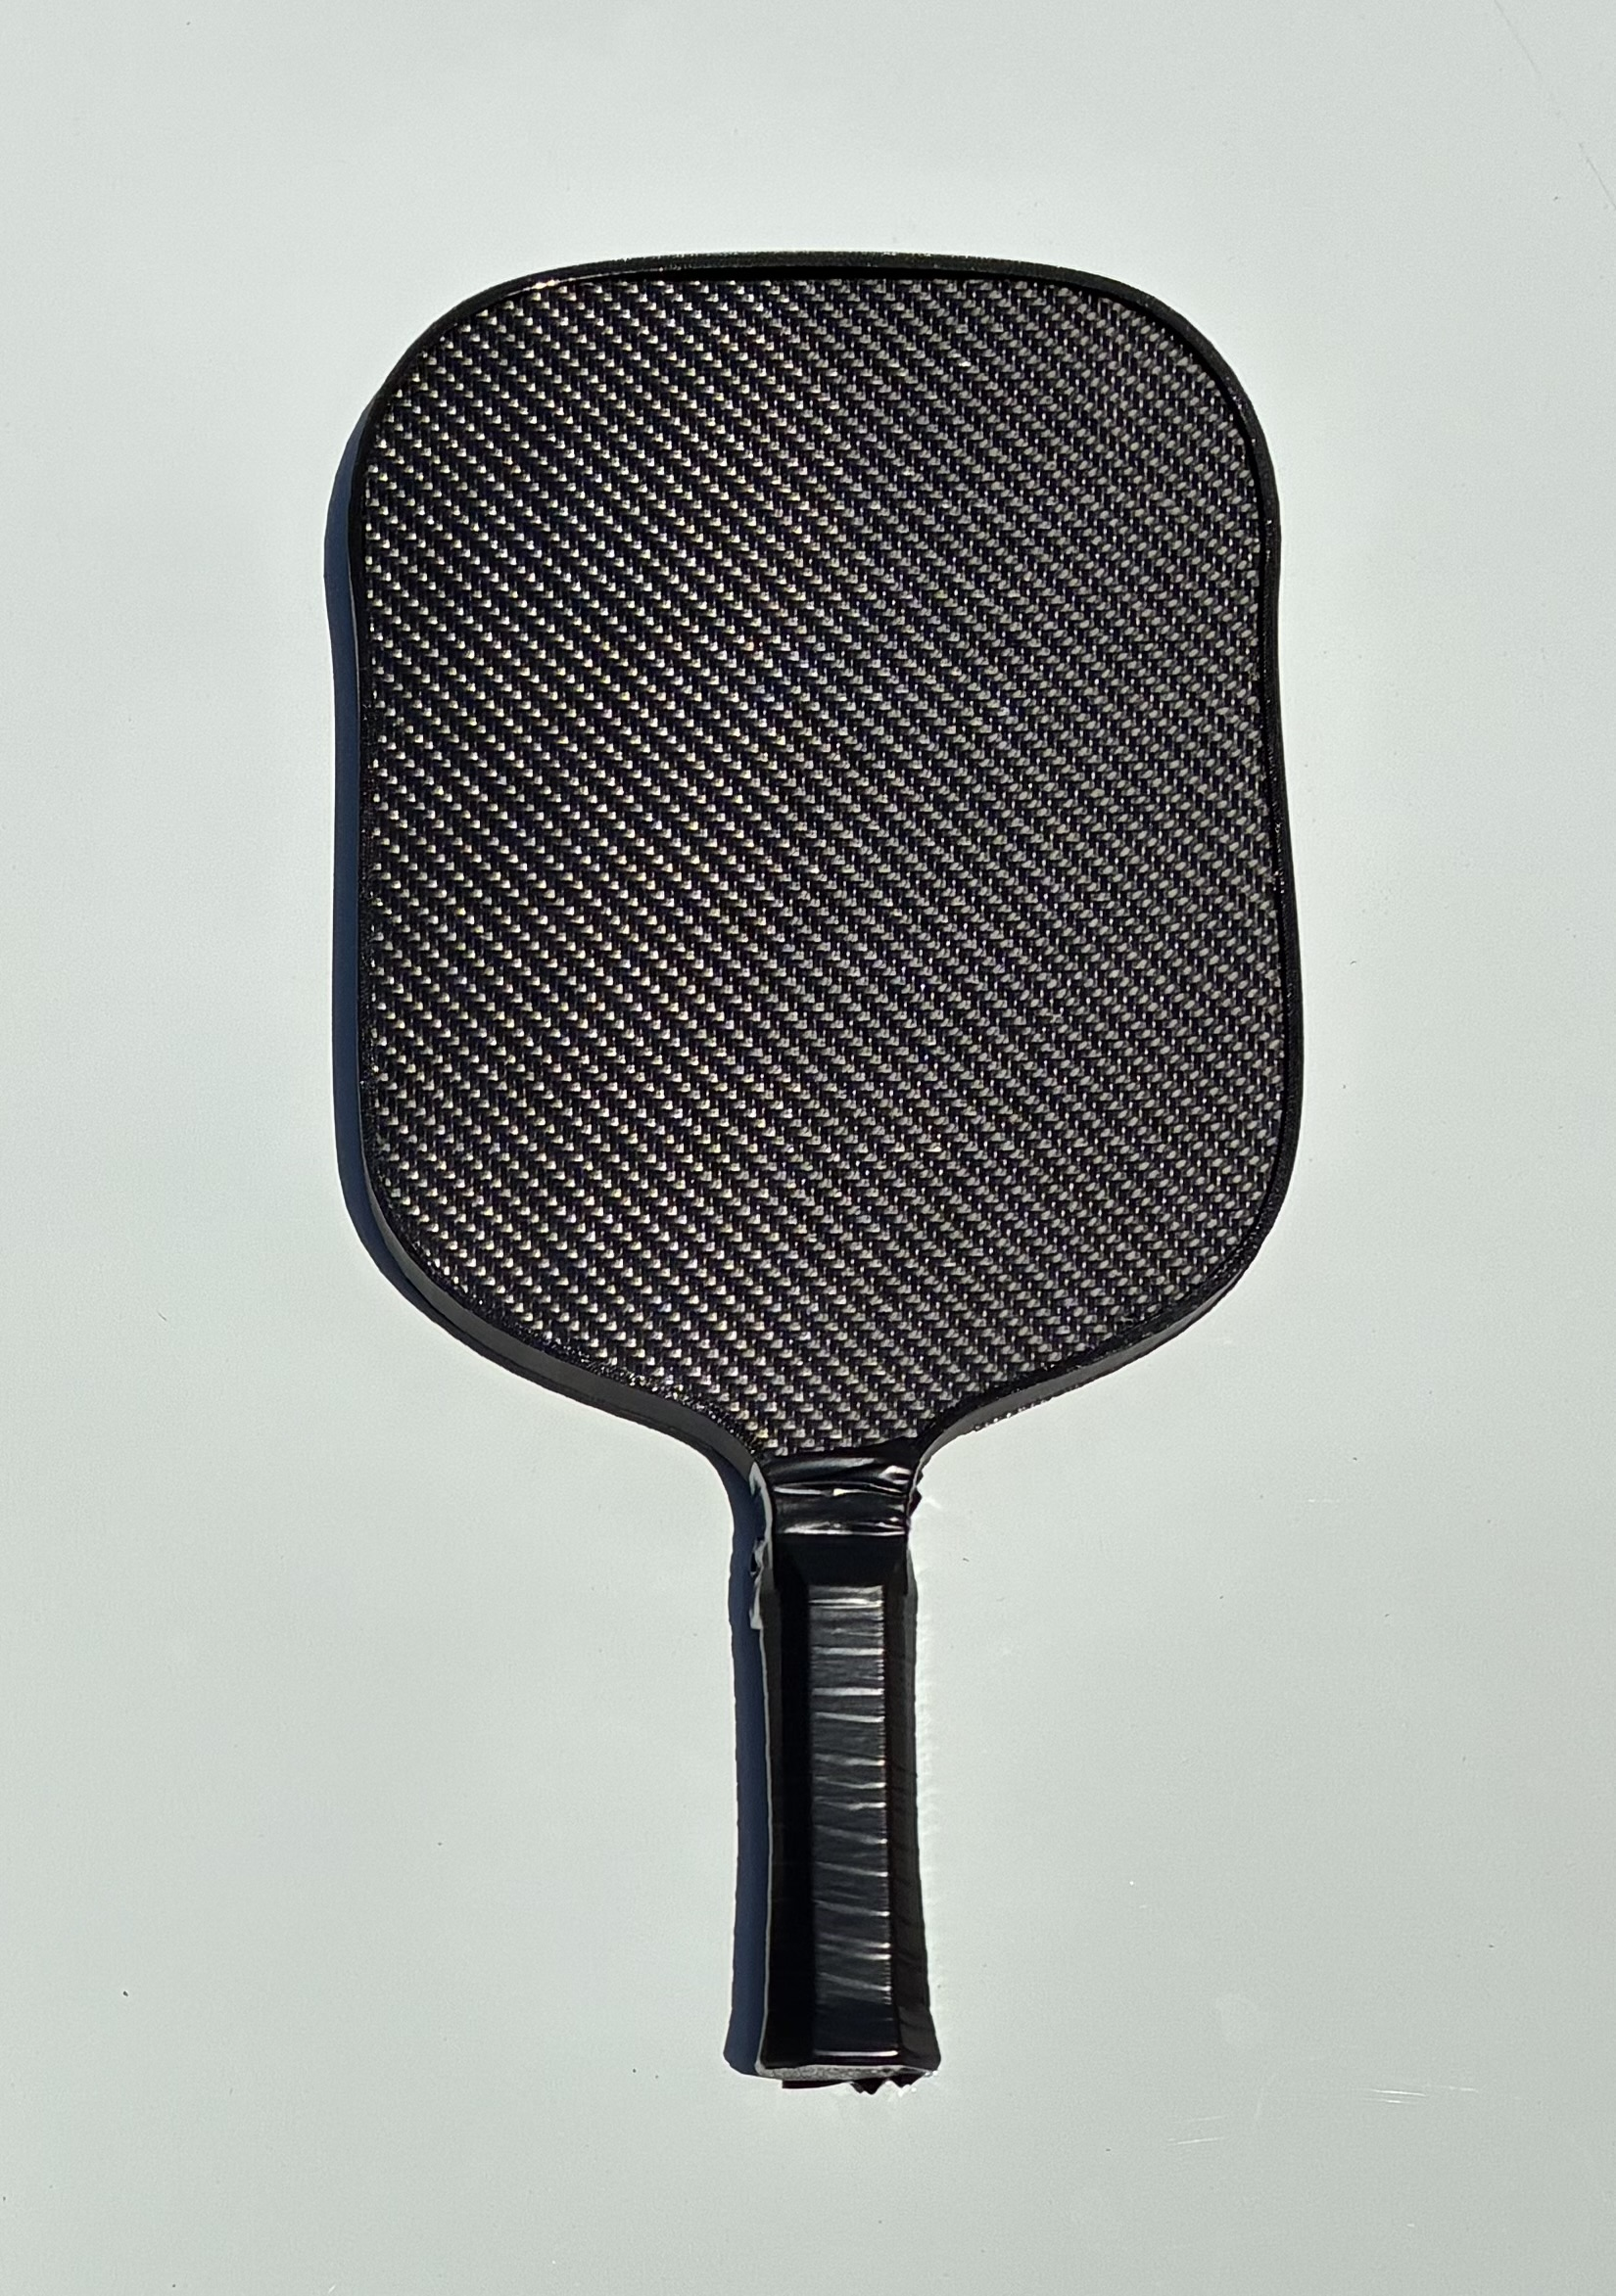
\includegraphics[
        width=3.72in,
        height=3.18in,
        keepaspectratio
    ]{full_assy}
};

\node[
    anchor=north,
    text=Muted,
    font=\sffamily\fontsize{6.9}{7.5}\selectfont
]
at ($(current page.north west)+(1.60in,-4.86in)$)
{Completed solo-built paddle assembly};

% ============================================================
% TOP CENTER — PROJECT OVERVIEW
% ============================================================

\fill[SoftGold,rounded corners=5pt]
    ($(current page.north west)+(2.95in,-1.62in)$)
    rectangle
    ($(current page.north west)+(5.53in,-4.86in)$);

\fill[PolyGold]
    ($(current page.north west)+(2.95in,-1.62in)$)
    rectangle
    ($(current page.north west)+(3.05in,-4.86in)$);

\node[
    anchor=north west,
    text=DeepGreen,
    font=\sffamily\bfseries\fontsize{8.0}{8.7}\selectfont
]
at ($(current page.north west)+(3.23in,-1.79in)$)
{PROJECT OVERVIEW};

\node[
    anchor=north west,
    align=left,
    text width=2.02in,
    text=Ink,
    font=\fontsize{7.05}{8.35}\selectfont
]
at ($(current page.north west)+(3.23in,-2.07in)$)
{
Independently designed and manufactured a lightweight prepreg
carbon-fiber pickleball paddle using a half-inch honeycomb
sandwich core, vacuum-bag consolidation, precision waterjet
trimming, and custom TPU and PLA components.

\vspace{5pt}

The project emphasized lightweight sandwich-composite design, repeatable manufacturing methods, dimensional accuracy, and the integration of custom 3D-printed TPU and PLA components into the final assembly.
};

\node[
    anchor=south west,
    align=left,
    text width=2.02in,
    text=PolyGold,
    font=\sffamily\bfseries\fontsize{6.65}{7.35}\selectfont
]
at ($(current page.north west)+(3.23in,-4.74in)$)
{
SOLE DESIGNER\\[2pt]
COMPOSITE FABRICATOR\\[2pt]
MANUFACTURING ENGINEER
};

% ============================================================
% TOP RIGHT — LAMINATE GRAPHIC
% ============================================================

\node[
    anchor=north west,
    inner sep=2.5pt,
    draw=DeepGreen,
    line width=0.65pt,
    rounded corners=5pt
]
at ($(current page.north west)+(5.71in,-1.62in)$)
{
    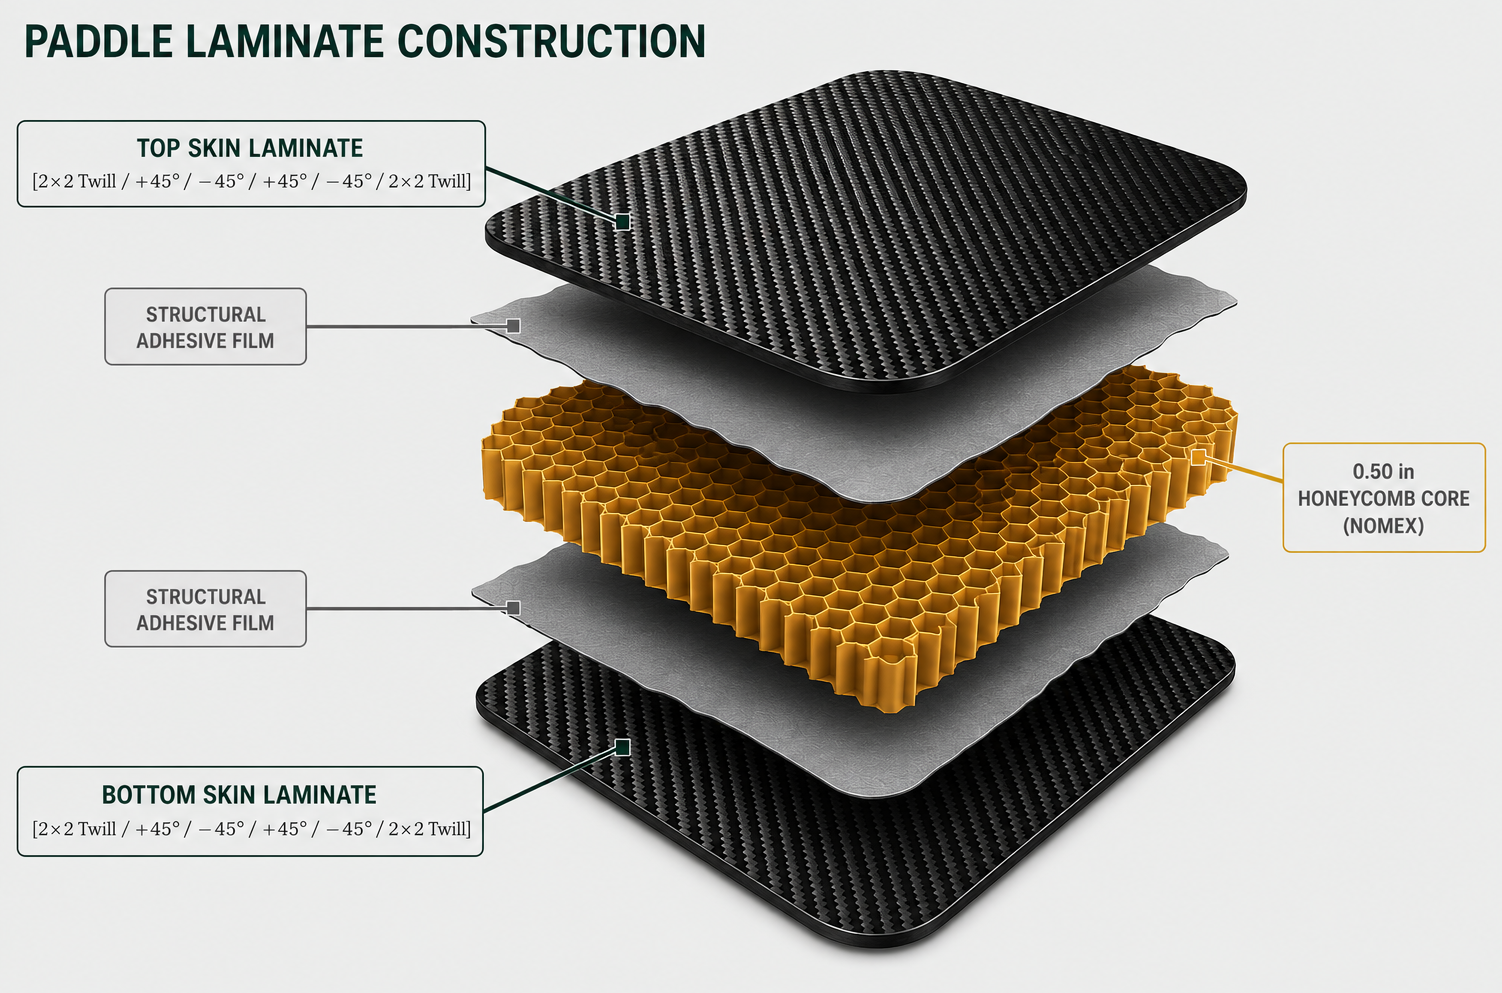
\includegraphics[
        width=4.80in,
        keepaspectratio
    ]{LAMINATE}
};

% ============================================================
% BOTTOM LEFT — SUPPORTING IMAGES
% ============================================================

\node[
    anchor=center,
    inner sep=3pt,
    draw=RuleGray,
    line width=0.55pt,
    rounded corners=4pt
]
at ($(current page.north west)+(1.12in,-5.98in)$)
{
    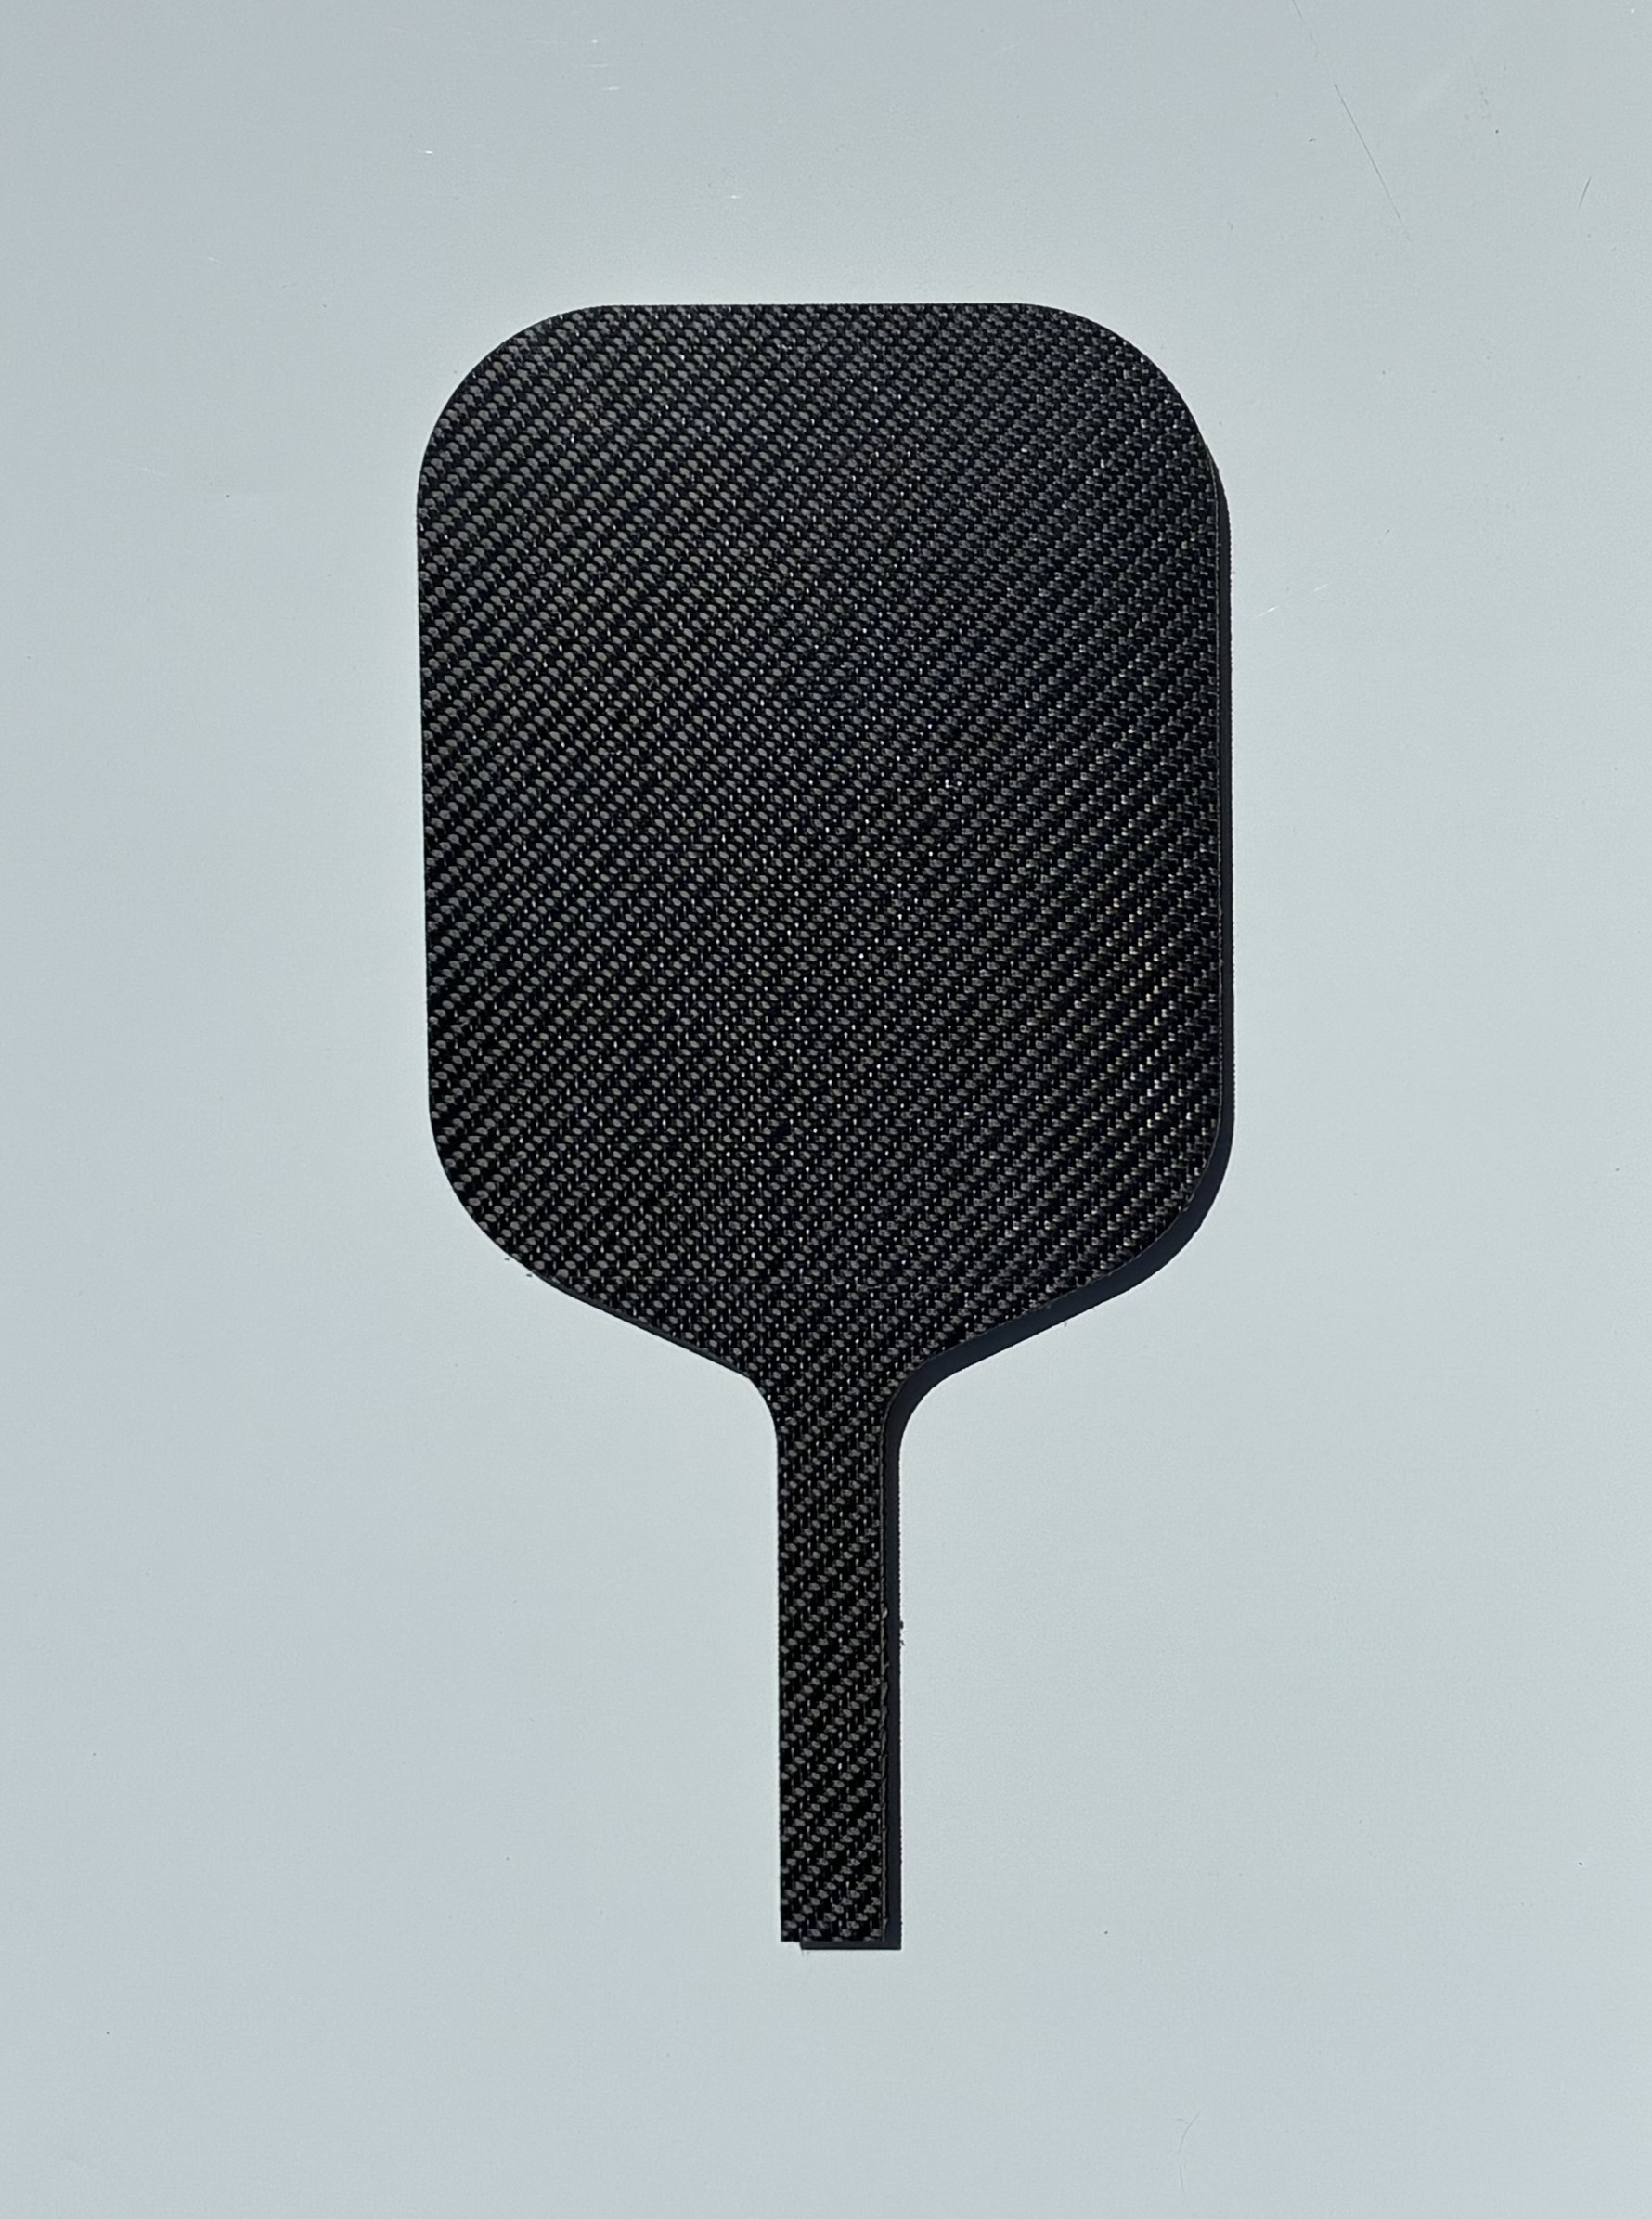
\includegraphics[
        width=1.30in,
        height=1.78in,
        keepaspectratio
    ]{front_view}
};

\node[
    anchor=center,
    inner sep=3pt,
    draw=RuleGray,
    line width=0.55pt,
    rounded corners=4pt
]
at ($(current page.north west)+(2.72in,-5.98in)$)
{
    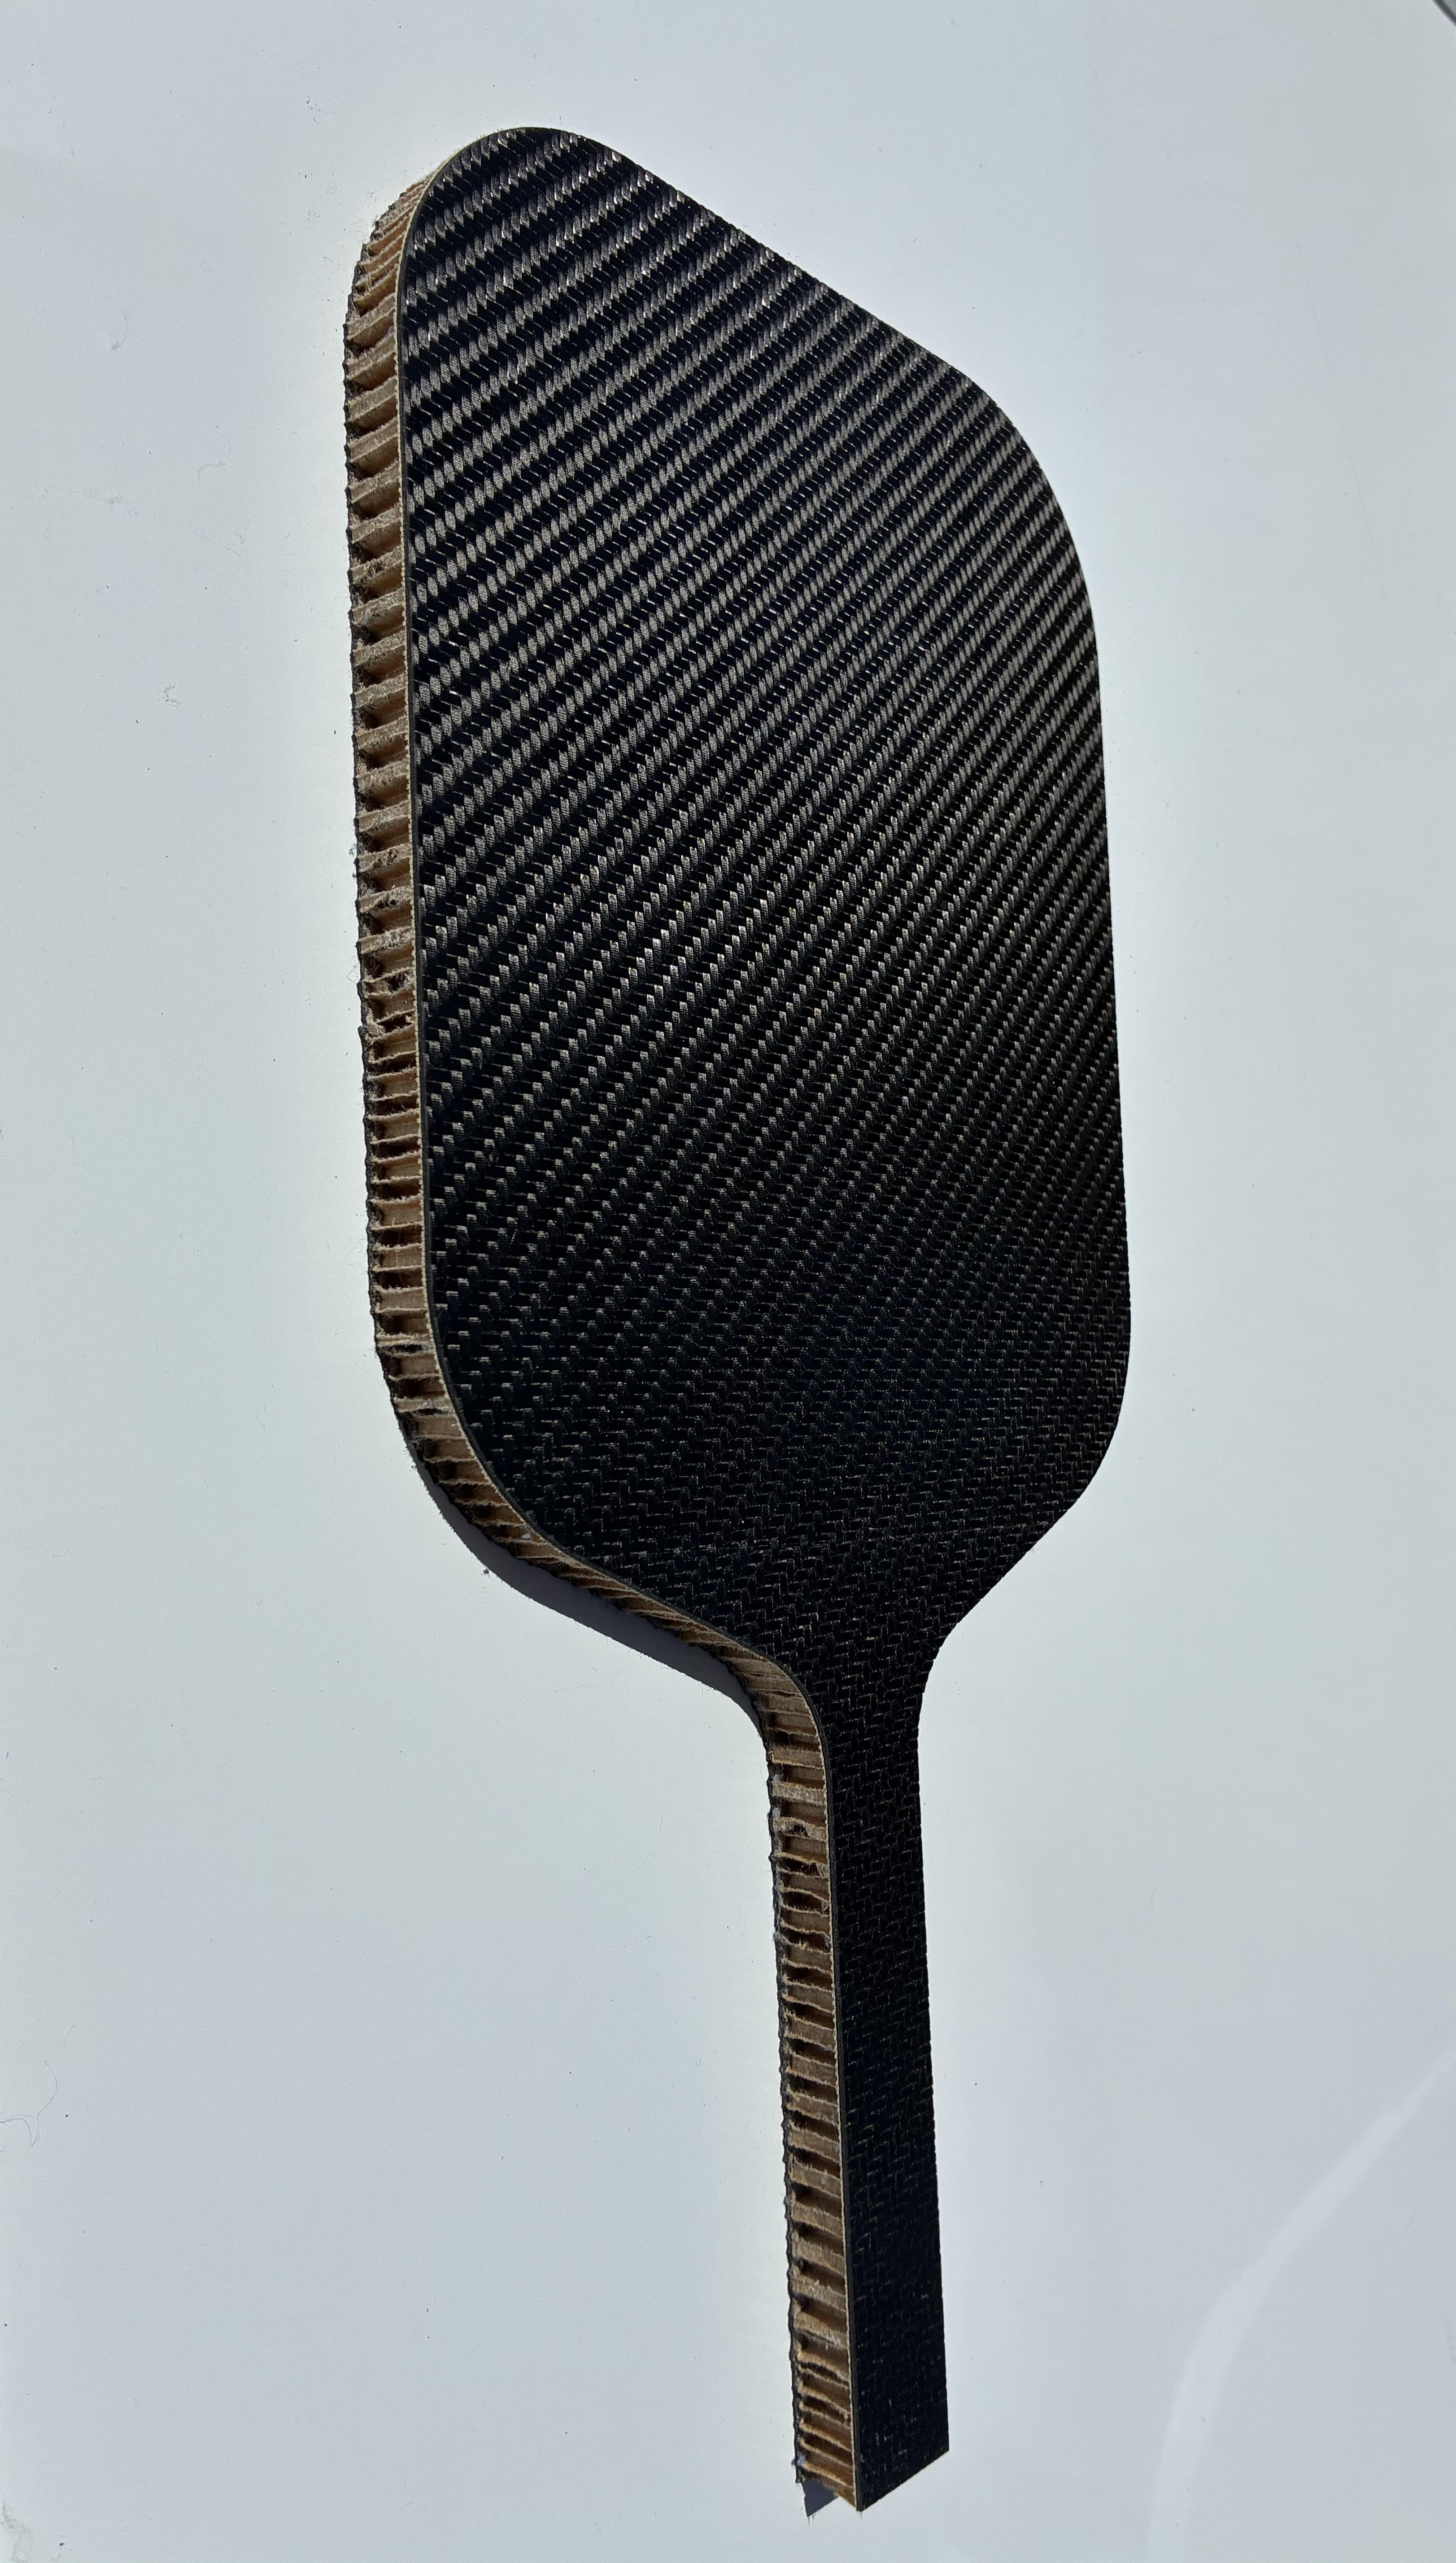
\includegraphics[
        width=1.30in,
        height=1.78in,
        keepaspectratio
    ]{side_core_view}
};

\node[
    anchor=center,
    inner sep=3pt,
    draw=RuleGray,
    line width=0.55pt,
    rounded corners=4pt
]
at ($(current page.north west)+(4.32in,-5.98in)$)
{
    \includegraphics[
        angle=-90,
        origin=c,
        width=1.30in,
        height=1.78in,
        keepaspectratio
    ]{waterjet}
};

\node[
    anchor=north,
    align=center,
    text width=1.38in,
    text=Muted,
    font=\sffamily\fontsize{6.5}{7.1}\selectfont
]
at ($(current page.north west)+(1.12in,-7.00in)$)
{Front view};

\node[
    anchor=north,
    align=center,
    text width=1.38in,
    text=Muted,
    font=\sffamily\fontsize{6.5}{7.1}\selectfont
]
at ($(current page.north west)+(2.72in,-7.00in)$)
{Core and edge profile};

\node[
    anchor=north,
    align=center,
    text width=1.38in,
    text=Muted,
    font=\sffamily\fontsize{6.5}{7.1}\selectfont
]
at ($(current page.north west)+(4.32in,-7.00in)$)
{Waterjet cutting setup};

% ============================================================
% BOTTOM RIGHT — MANUFACTURING HIGHLIGHTS
% ============================================================

\fill[SoftGreen,rounded corners=5pt]
    ($(current page.north west)+(5.18in,-5.05in)$)
    rectangle
    ($(current page.north east)+(-0.42in,-7.18in)$);

\draw[RuleGray,line width=0.55pt,rounded corners=5pt]
    ($(current page.north west)+(5.18in,-5.05in)$)
    rectangle
    ($(current page.north east)+(-0.42in,-7.18in)$);

\node[
    anchor=north west,
    text=DeepGreen,
    font=\sffamily\bfseries\fontsize{7.9}{8.6}\selectfont
]
at ($(current page.north west)+(5.44in,-5.20in)$)
{MANUFACTURING HIGHLIGHTS};

\node[
    anchor=north west,
    align=left,
    text width=5.05in,
    text=Ink,
    font=\fontsize{6.72}{7.82}\selectfont
]
at ($(current page.north west)+(5.44in,-5.49in)$)
{
\textbf{Consolidation.}
Vacuum bagging and distributed weight pressure maintained intimate contact
throughout the prepreg sandwich layup.\\[2.4pt]
\textbf{Surface quality.}
A scarce PTFE release film produced an unusually consistent matte finish
with a subtle sheen and minimal post-processing.\\[2.4pt]
\textbf{Waterjet stability.}
Perimeter weights restrained the cured stock against jet-induced lifting
and rotational moments during cutting.\\[2.4pt]
\textbf{Final assembly.}
A printed TPU edge band protected the carbon perimeter, while the PLA handle
used clearance cutouts to accommodate future stock-thickness and cutting variation.
};

% ============================================================
% RESOURCE LINK
% ============================================================

\node[
    anchor=north,
    align=center,
    text=DeepGreen,
    font=\sffamily\bfseries\fontsize{7.0}{7.6}\selectfont
]
at ($(current page.north)+(0,-7.42in)$)
{\href{\PaddleWaterjetVideo}
{\faPlayCircle\ WATERJET PICKLEBALL PADDLE DEMONSTRATION}};

% ============================================================
% FOOTER
% ============================================================

\node[
    anchor=south west,
    text=white,
    font=\sffamily\bfseries\fontsize{7.1}{7.7}\selectfont
]
at ($(current page.south west)+(0.42in,0.17in)$)
{\hyperlink{toro-results}{\faArrowLeft\ TORO COVER}};

\node[
    anchor=south,
    text=white,
    font=\sffamily\fontsize{7.0}{7.6}\selectfont
]
at ($(current page.south)+(0,0.17in)$)
{PICKLEBALL PADDLE \hspace{6pt} 1 / 1};

\node[
    anchor=south east,
    text=white,
    font=\sffamily\bfseries\fontsize{7.1}{7.7}\selectfont
]
at ($(current page.south east)+(-0.42in,0.17in)$)
{NEXT PROJECT \faArrowRight};

\end{tikzpicture}
%\input{Beam}
%\clearpage

\clearpage
 before \end{document}.
% 3. Image references use the original Overleaf base filenames
%    without extensions.
% ============================================================



% ============================================================
% CLICKABLE PROJECT RESOURCES
% All links use the exact Google Drive resources supplied.
% ============================================================
\providecommand{\ToroDrawingLink}{https://drive.google.com/file/d/1A7-7wMnRNLuQDaTgxeuUCBsGNqyXzOGV/view?usp=sharing}
\providecommand{\ToroDimensionsLink}{https://drive.google.com/file/d/13sw3BNJvE8GdzlRffxoF2n5r9Gzxide7/view?usp=sharing}
\providecommand{\ToroProblemLink}{https://drive.google.com/file/d/1zHtl8zrb13F1yeN74ptawpfS5UM_xsuw/view?usp=drive_link}
\providecommand{\ToroReportLink}{https://drive.google.com/file/d/1ULZ-P46lFsC2x29ZfmRVIKgYnr9o8hMt/view?usp=drive_link}
\providecommand{\ToroPosterLink}{https://drive.google.com/file/d/1vKiKaJUcHQb_db-FkZnRF6EvtuM4hKyS/view?usp=drive_link}
\providecommand{\ToroDeploymentLink}{https://drive.google.com/file/d/1XJx34o80_mZPTl7xy93HtWAgtS3ThhvY/view?usp=drive_link}
\providecommand{\ToroRemovalLink}{https://drive.google.com/file/d/1O7xYeyB67NUwT-j1B1HeiCcHnZDYjk6_/view?usp=drive_link}

% ============================================================
% PAGE 1 — PROJECT OVERVIEW, OWNERSHIP, AND ARCHITECTURE
% ============================================================

\clearpage
\thispagestyle{empty}
\hypertarget{toro}{}
\null

\begin{tikzpicture}[remember picture,overlay]

% Background
\fill[white]
    (current page.south west)
    rectangle
    (current page.north east);

% Page bars
\fill[DeepGreen]
    (current page.north west)
    rectangle
    ($(current page.north east)+(0,-0.095in)$);

\fill[PolyGold]
    ($(current page.north west)+(0,-0.095in)$)
    rectangle
    ($(current page.north east)+(0,-0.14in)$);

\fill[DeepGreen]
    (current page.south west)
    rectangle
    ($(current page.south east)+(0,0.36in)$);

\fill[PolyGold]
    ($(current page.south west)+(0,0.36in)$)
    rectangle
    ($(current page.south east)+(0,0.405in)$);

% Header
\node[
    anchor=north west,
    text=PolyGold,
    font=\sffamily\bfseries\fontsize{8.1}{8.7}\selectfont
]
at ($(current page.north west)+(0.42in,-0.39in)$)
{01 COMPOSITES \hspace{5pt}/\hspace{5pt} PROJECT 01};

\node[
    anchor=north west,
    text=DeepGreen,
    font=\bfseries\fontsize{23.5}{24.5}\selectfont
]
at ($(current page.north west)+(0.40in,-0.67in)$)
{TORO CARBON FIBER SAFETY COVER};

\node[
    anchor=north west,
    text=Muted,
    font=\sffamily\fontsize{8.4}{9.2}\selectfont
]
at ($(current page.north west)+(0.42in,-1.12in)$)
{Cal Poly Composites Laboratory \hspace{7pt}\textbullet\hspace{7pt}
Team Project \hspace{7pt}\textbullet\hspace{7pt}
Fall--Spring 2026 \hspace{7pt}\textbullet\hspace{7pt}
San Luis Obispo, California};

\fill[PolyGold]
    ($(current page.north west)+(0.42in,-1.37in)$)
    rectangle
    ($(current page.north west)+(6.1in,-1.325in)$);

% Challenge text
\node[
    anchor=north west,
    text=DeepGreen,
    font=\sffamily\bfseries\fontsize{8.1}{8.8}\selectfont
]
at ($(current page.north west)+(0.43in,-1.61in)$)
{THE CHALLENGE};

\node[
    anchor=north west,
    align=left,
    text width=4.47in,
    text=Ink,
    font=\fontsize{8.05}{9.65}\selectfont
]
at ($(current page.north west)+(0.43in,-1.84in)$)
{
Develop a lightweight cover for a 6 ft by 6 ft in-ground spa
that could be deployed by one person, stored compactly,
provide insulation, resist a poolside environment, and maintain
a refined appearance. The sponsor supplied an ambitious but
intentionally broad project statement, requiring the team to
define the product architecture, priorities, manufacturing
strategy, and realistic path toward future commercialization.
};

% Role box
\fill[SoftGold,rounded corners=5pt]
    ($(current page.north west)+(0.42in,-2.88in)$)
    rectangle
    ($(current page.north west)+(4.98in,-4.58in)$);

\fill[PolyGold]
    ($(current page.north west)+(0.42in,-2.88in)$)
    rectangle
    ($(current page.north west)+(0.52in,-4.58in)$);

\node[
    anchor=north west,
    text=DeepGreen,
    font=\sffamily\bfseries\fontsize{8.1}{8.8}\selectfont
]
at ($(current page.north west)+(0.66in,-3.02in)$)
{MY ROLE — DESIGN \& MANUFACTURING LEAD};

\node[
    anchor=north west,
    align=left,
    text width=4.02in,
    text=Ink,
    font=\fontsize{7.05}{8.15}\selectfont
]
at ($(current page.north west)+(0.66in,-3.27in)$)
{
\textbullet\ Modeled every custom part and the complete assembly\\[1.5pt]
\textbullet\ Produced the engineering drawing package independently\\[1.5pt]
\textbullet\ Developed the composite-panel manufacturing process\\[1.5pt]
\textbullet\ Created all waterjet DXFs and manufacturing geometry\\[1.5pt]
\textbullet\ Trained teammates in wet layup and vacuum bagging\\[1.5pt]
\textbullet\ Presented feasibility, scope, and tradeoffs to the sponsor
};

% Large deployed foam-model image
\node[anchor=center,inner sep=0pt]
at ($(current page.north west)+(8.00in,-3.04in)$)
{
    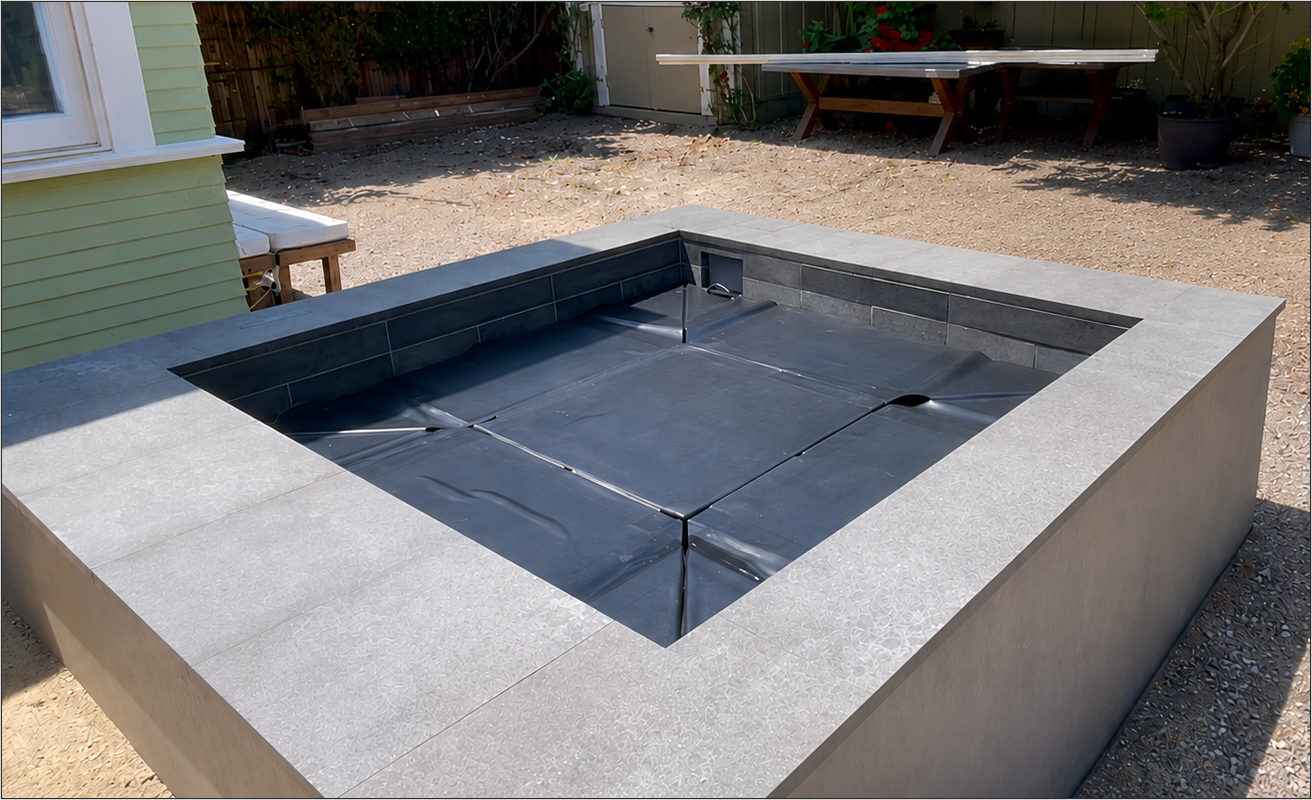
\includegraphics[
        width=5.55in,
        height=2.78in,
        keepaspectratio
    ]{deployed_functional_prototype}
};

\draw[DeepGreen,line width=0.8pt,rounded corners=7pt]
    ($(current page.north west)+(5.16in,-1.61in)$)
    rectangle
    ($(current page.north east)+(-0.42in,-4.47in)$);

\node[
    anchor=north west,
    text=Muted,
    font=\sffamily\fontsize{6.2}{6.9}\selectfont
]
at ($(current page.north west)+(5.18in,-4.54in)$)
{Functional foam model deployed over the sponsor's in-ground spa.};

% Image-strip title
\node[
    anchor=north west,
    text=DeepGreen,
    font=\sffamily\bfseries\fontsize{8.1}{8.8}\selectfont
]
at ($(current page.north west)+(0.43in,-4.78in)$)
{PRODUCT DEVELOPMENT AND FINAL ARCHITECTURE};

% Five-image development strip — CAD-first sequence
% Image 1: topside CAD
\node[anchor=center,inner sep=0pt]
at ($(current page.north west)+(1.47in,-5.73in)$)
{
    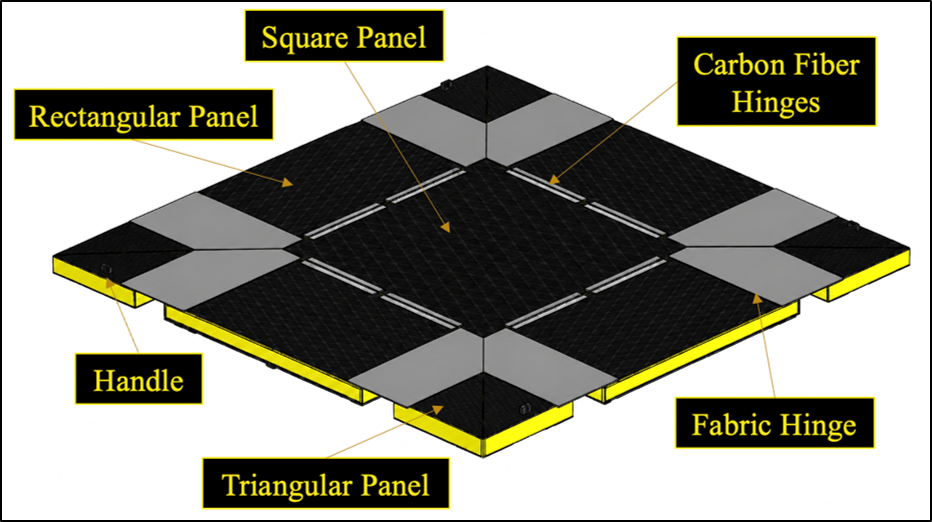
\includegraphics[
        width=1.92in,
        height=1.30in,
        keepaspectratio
    ]{Toro_Cover_topside_Cad}
};
\draw[RuleGray,line width=0.55pt,rounded corners=4pt]
    ($(current page.north west)+(0.43in,-5.04in)$)
    rectangle
    ($(current page.north west)+(2.51in,-6.43in)$);

% Image 2: underside CAD
\node[anchor=center,inner sep=0pt]
at ($(current page.north west)+(3.66in,-5.73in)$)
{
    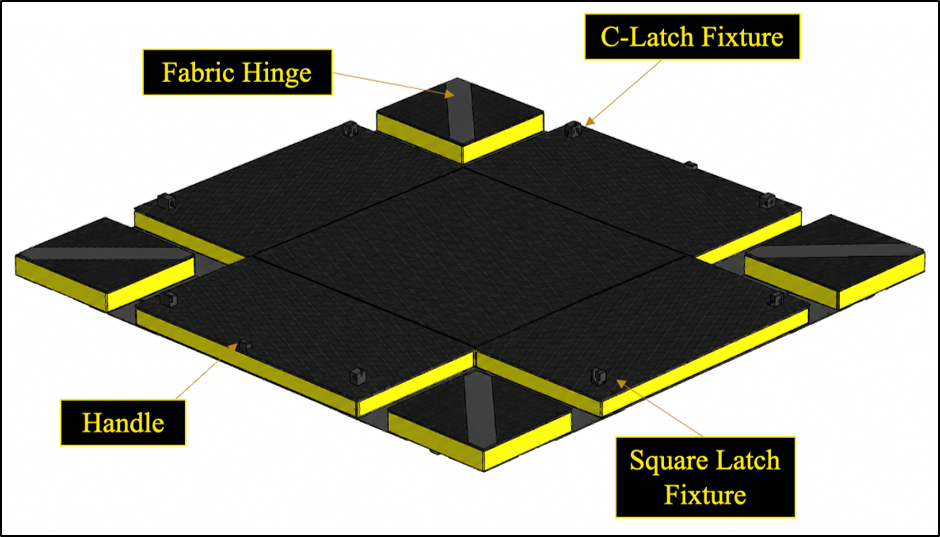
\includegraphics[
        width=1.92in,
        height=1.30in,
        keepaspectratio
    ]{toro_cover_underside_cad}
};
\draw[RuleGray,line width=0.55pt,rounded corners=4pt]
    ($(current page.north west)+(2.62in,-5.04in)$)
    rectangle
    ($(current page.north west)+(4.70in,-6.43in)$);

% Image 3: folded CAD
\node[anchor=center,inner sep=0pt]
at ($(current page.north west)+(5.85in,-5.73in)$)
{
    \includegraphics[
        width=1.92in,
        height=1.30in,
        keepaspectratio
    ]{\detokenize{Toro_Cover_folded Configuration}}
};
\draw[RuleGray,line width=0.55pt,rounded corners=4pt]
    ($(current page.north west)+(4.81in,-5.04in)$)
    rectangle
    ($(current page.north west)+(6.89in,-6.43in)$);

% Image 4: dual-use product concept
\node[anchor=center,inner sep=0pt]
at ($(current page.north west)+(8.04in,-5.73in)$)
{
    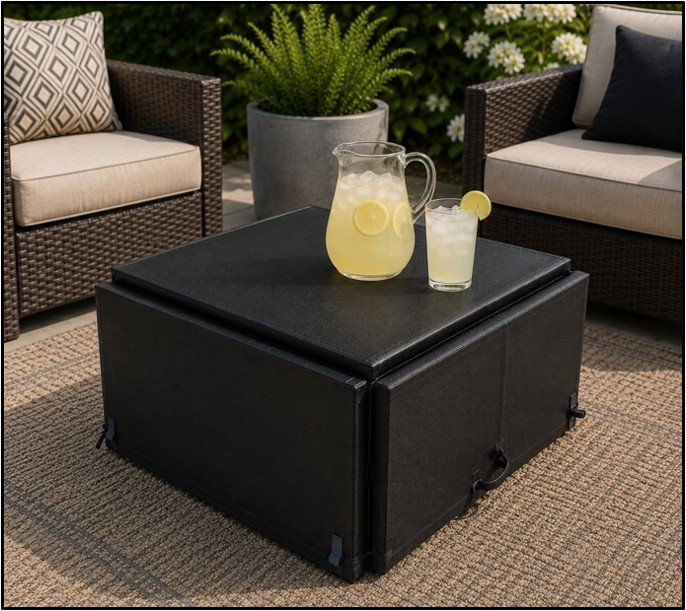
\includegraphics[
        width=1.92in,
        height=1.30in,
        keepaspectratio
    ]{generative_AI_concept_toro_cover_art}
};
\draw[RuleGray,line width=0.55pt,rounded corners=4pt]
    ($(current page.north west)+(7.00in,-5.04in)$)
    rectangle
    ($(current page.north west)+(9.08in,-6.43in)$);

% Image 5: folded foam functional prototype
% The portrait photograph is deliberately clipped to the landscape frame
% so the ottoman fills the card without extending beyond its border.
\begin{scope}
\clip[rounded corners=4pt]
    ($(current page.north west)+(9.19in,-5.04in)$)
    rectangle
    ($(current page.north east)+(-0.43in,-6.43in)$);

% Keep the original image proportions and center it within the existing card.
\node[anchor=center,inner sep=0pt]
at ($(current page.north west)+(9.88in,-5.735in)$)
{
    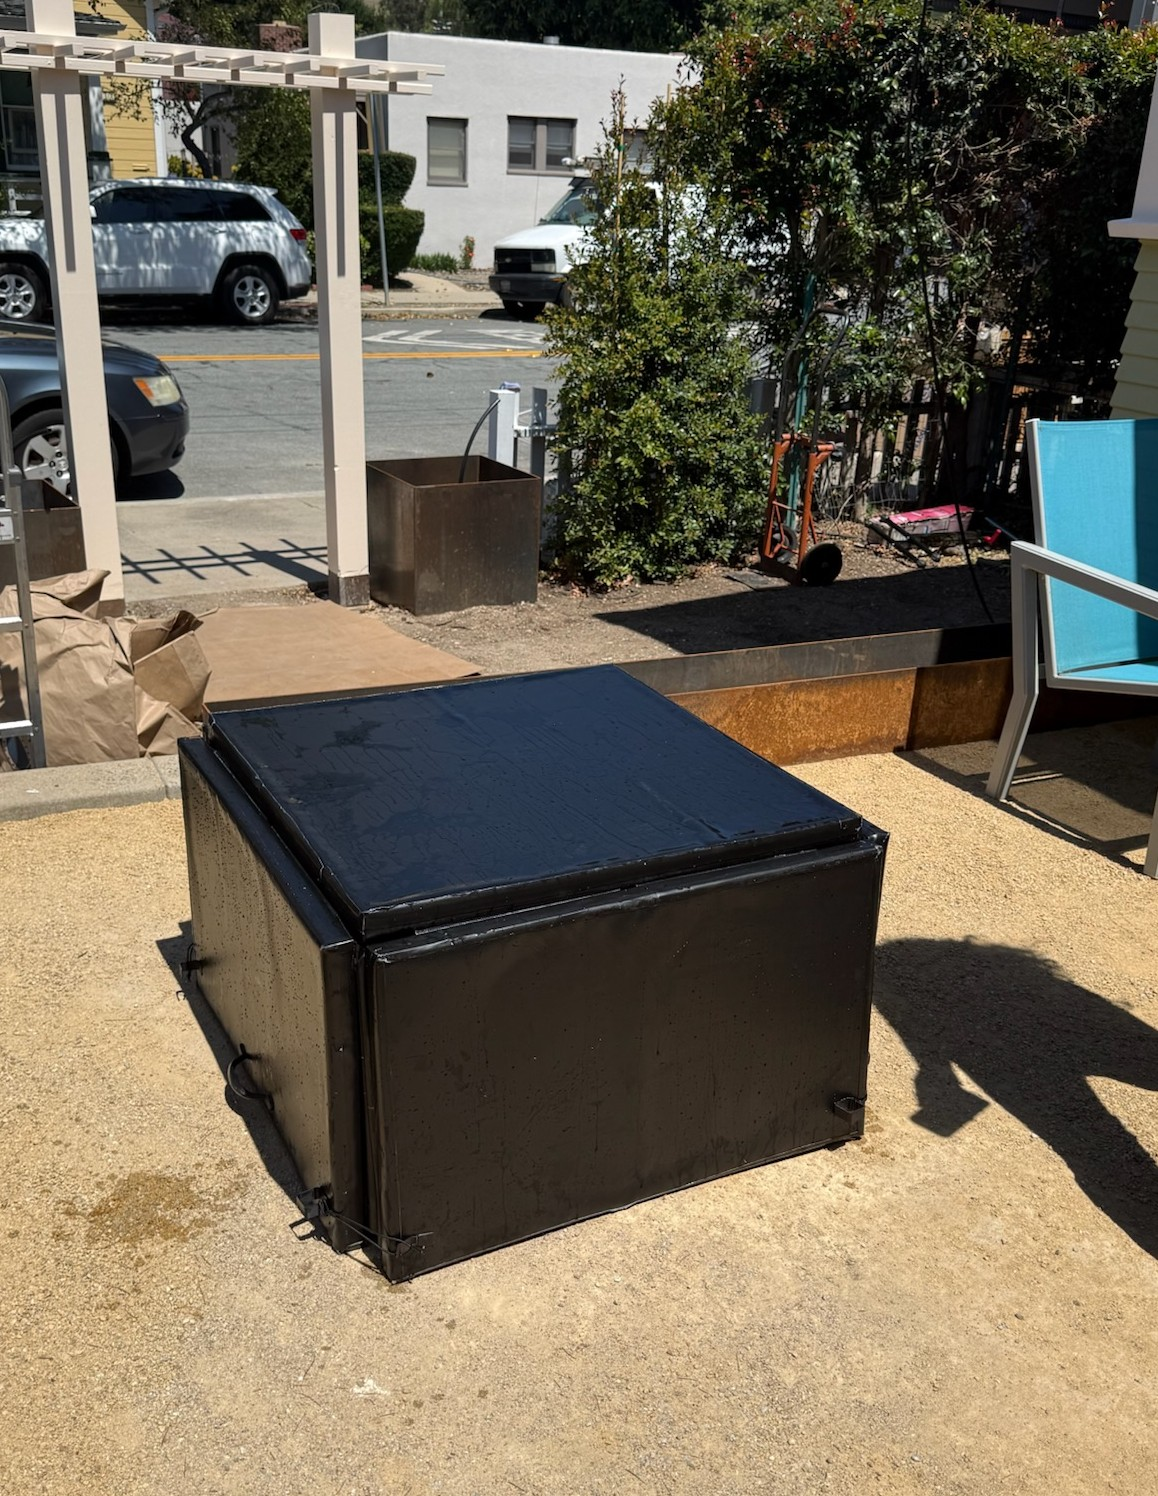
\includegraphics[
        width=1.58in,
        height=1.28in,
        keepaspectratio
    ]{foam_model_folded_backyard_image}
};
\end{scope}

\draw[RuleGray,line width=0.55pt,rounded corners=4pt]
    ($(current page.north west)+(9.19in,-5.04in)$)
    rectangle
    ($(current page.north east)+(-0.43in,-6.43in)$);

% Larger captions
\node[anchor=north,align=center,text width=1.95in,text=Muted,
      font=\sffamily\fontsize{6.8}{7.4}\selectfont]
at ($(current page.north west)+(1.47in,-6.49in)$)
{Topside panel architecture};

\node[anchor=north,align=center,text width=1.95in,text=Muted,
      font=\sffamily\fontsize{6.8}{7.4}\selectfont]
at ($(current page.north west)+(3.66in,-6.49in)$)
{Underside hinge architecture};

\node[anchor=north,align=center,text width=1.95in,text=Muted,
      font=\sffamily\fontsize{6.8}{7.4}\selectfont]
at ($(current page.north west)+(5.85in,-6.49in)$)
{Folded CAD configuration};

\node[anchor=north,align=center,text width=1.95in,text=Muted,
      font=\sffamily\fontsize{6.8}{7.4}\selectfont]
at ($(current page.north west)+(8.04in,-6.49in)$)
{Dual-use product vision};

\node[anchor=north,align=center,text width=1.95in,text=Muted,
      font=\sffamily\fontsize{6.8}{7.4}\selectfont]
at ($(current page.north west)+(9.88in,-6.49in)$)
{Folded foam prototype};

% Page 1 resource bar — centered and non-repeated resources
\fill[Panel,rounded corners=4pt]
    ($(current page.north west)+(0.43in,-7.05in)$)
    rectangle
    ($(current page.north east)+(-0.43in,-7.64in)$);
\draw[RuleGray,line width=0.5pt,rounded corners=4pt]
    ($(current page.north west)+(0.43in,-7.05in)$)
    rectangle
    ($(current page.north east)+(-0.43in,-7.64in)$);

\node[
    anchor=center,
    align=center,
    text=DeepGreen,
    font=\sffamily\bfseries\fontsize{6.9}{7.5}\selectfont
]
at ($(current page.north)+(0,-7.345in)$)
{\href{\ToroDrawingLink}{\faDraftingCompass\ DRAWING PACKAGE}
\hspace{24pt}
\href{\ToroDimensionsLink}{\faImage\ DIMENSION STUDY}
\hspace{24pt}
\href{\ToroProblemLink}{\faFileImage\ PROBLEM STATEMENT}};

% Footer
\node[
    anchor=south west,
    text=white,
    font=\sffamily\bfseries\fontsize{7.1}{7.7}\selectfont
]
at ($(current page.south west)+(0.42in,0.17in)$)
{\hyperlink{composites}{\faArrowLeft\ COMPOSITES}};

\node[
    anchor=south,
    text=white,
    font=\sffamily\fontsize{7.0}{7.6}\selectfont
]
at ($(current page.south)+(0,0.17in)$)
{TORO COVER \hspace{6pt} 1 / 3};

\node[
    anchor=south east,
    text=white,
    font=\sffamily\bfseries\fontsize{7.1}{7.7}\selectfont
]
at ($(current page.south east)+(-0.42in,0.17in)$)
{MANUFACTURING-DRIVEN DESIGN \faArrowRight};

\end{tikzpicture}


% ============================================================
% PAGE 2 — MANUFACTURING-DRIVEN DESIGN
% ============================================================

\clearpage
\thispagestyle{empty}
\hypertarget{toro-manufacturing}{}
\null

\begin{tikzpicture}[remember picture,overlay]

% Background and bars
\fill[white]
    (current page.south west)
    rectangle
    (current page.north east);

\fill[DeepGreen]
    (current page.north west)
    rectangle
    ($(current page.north east)+(0,-0.095in)$);

\fill[PolyGold]
    ($(current page.north west)+(0,-0.095in)$)
    rectangle
    ($(current page.north east)+(0,-0.14in)$);

\fill[DeepGreen]
    (current page.south west)
    rectangle
    ($(current page.south east)+(0,0.36in)$);

\fill[PolyGold]
    ($(current page.south west)+(0,0.36in)$)
    rectangle
    ($(current page.south east)+(0,0.405in)$);

% Header
\node[
    anchor=north west,
    text=PolyGold,
    font=\sffamily\bfseries\fontsize{8.1}{8.7}\selectfont
]
at ($(current page.north west)+(0.42in,-0.39in)$)
{TORO COVER \hspace{5pt}/\hspace{5pt} DESIGN FOR MANUFACTURABILITY};

\node[
    anchor=north west,
    text=DeepGreen,
    font=\bfseries\fontsize{23}{24}\selectfont
]
at ($(current page.north west)+(0.40in,-0.67in)$)
{THE ENVELOPE METHOD};

\node[
    anchor=north west,
    text=Muted,
    font=\sffamily\fontsize{8.7}{9.6}\selectfont
]
at ($(current page.north west)+(0.42in,-1.12in)$)
{A one-layup process developed for unusually thick insulated composite sandwich panels};

\fill[PolyGold]
    ($(current page.north west)+(0.42in,-1.36in)$)
    rectangle
    ($(current page.north west)+(5.30in,-1.315in)$);

% Process explanation
\fill[SoftGold,rounded corners=5pt]
    ($(current page.north west)+(0.42in,-1.61in)$)
    rectangle
    ($(current page.north east)+(-0.42in,-2.90in)$);

\fill[PolyGold]
    ($(current page.north west)+(0.42in,-1.61in)$)
    rectangle
    ($(current page.north west)+(0.52in,-2.90in)$);

\node[
    anchor=north west,
    text=DeepGreen,
    font=\sffamily\bfseries\fontsize{7.9}{8.6}\selectfont
]
at ($(current page.north west)+(0.67in,-1.76in)$)
{PROCESS INNOVATION};

\node[
    anchor=north west,
    align=left,
    text width=9.55in,
    text=Ink,
    font=\fontsize{7.35}{8.75}\selectfont
]
at ($(current page.north west)+(0.67in,-2.02in)$)
{
Weight reduction and insulation were both essential, leading to the selection of an
XPS foam core. Because XPS could not tolerate composite heat-cure temperatures, prepreg
processing was not practical and the panels had to be manufactured by wet layup with a
room-temperature cure. To simplify this process, I waterjet-cut XPS perimeter strips from
excess foam and placed them around each core inside the vacuum enclosure. Under vacuum,
the top and bottom carbon skins met along the panel sides and compressed against this
border, eliminating a separate edge-banding layup and reducing corner pleating.
};

% Workflow title
\node[
    anchor=north west,
    text=DeepGreen,
    font=\sffamily\bfseries\fontsize{8.0}{8.7}\selectfont
]
at ($(current page.north west)+(0.43in,-3.06in)$)
{MANUFACTURING WORKFLOW};

% Row 1 image 1
\node[anchor=center,inner sep=0pt]
at ($(current page.north west)+(2.07in,-4.105in)$)
{
    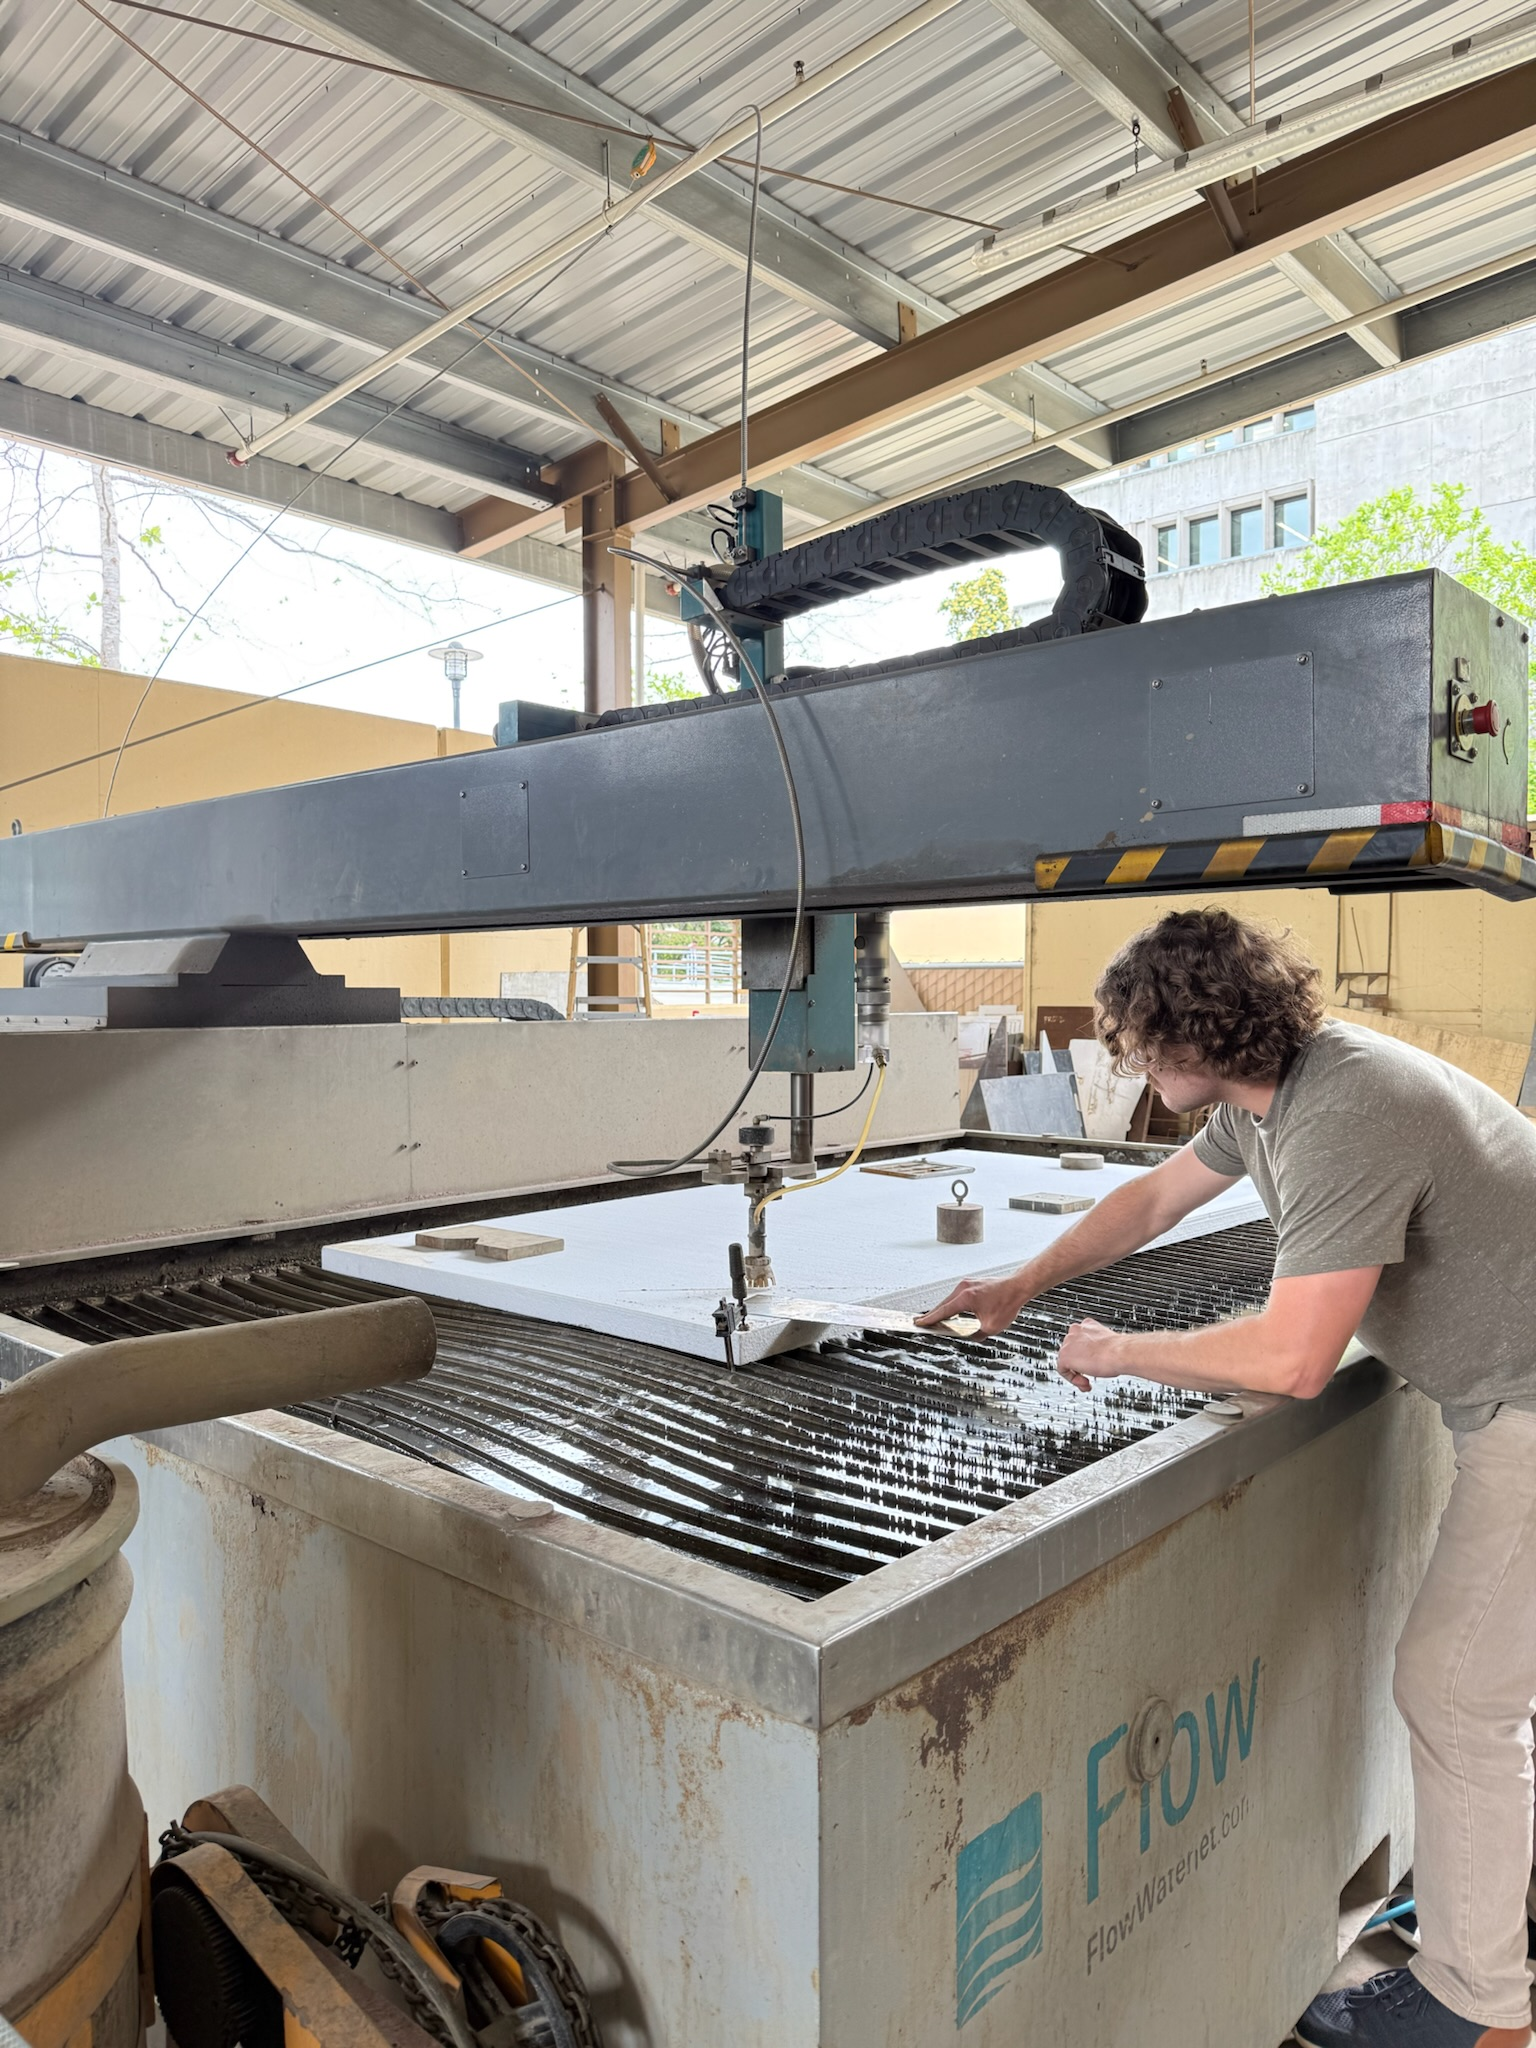
\includegraphics[
        width=3.10in,
        height=1.40in,
        keepaspectratio
    ]{waterjet_foam}
};
\draw[RuleGray,line width=0.55pt,rounded corners=4pt]
    ($(current page.north west)+(0.43in,-3.36in)$)
    rectangle
    ($(current page.north west)+(3.71in,-4.85in)$);

% Row 1 image 2
\node[anchor=center,inner sep=0pt]
at ($(current page.north west)+(5.50in,-4.105in)$)
{
    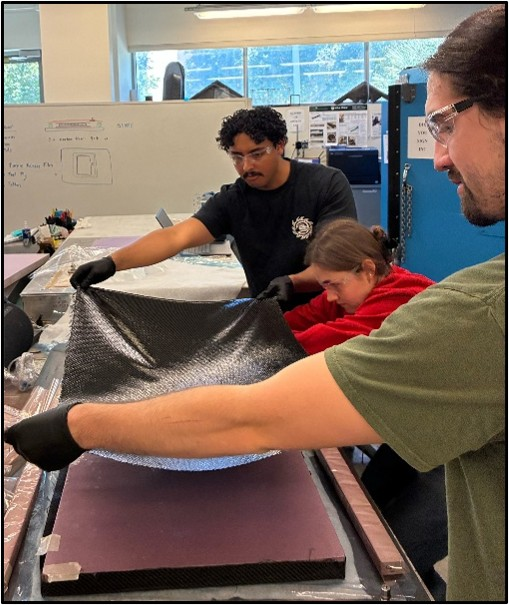
\includegraphics[
        width=3.10in,
        height=1.40in,
        keepaspectratio
    ]{group_layup}
};
\draw[RuleGray,line width=0.55pt,rounded corners=4pt]
    ($(current page.north west)+(3.86in,-3.36in)$)
    rectangle
    ($(current page.north west)+(7.14in,-4.85in)$);

% Row 1 image 3
\node[anchor=center,inner sep=0pt]
at ($(current page.north west)+(8.935in,-4.105in)$)
{
    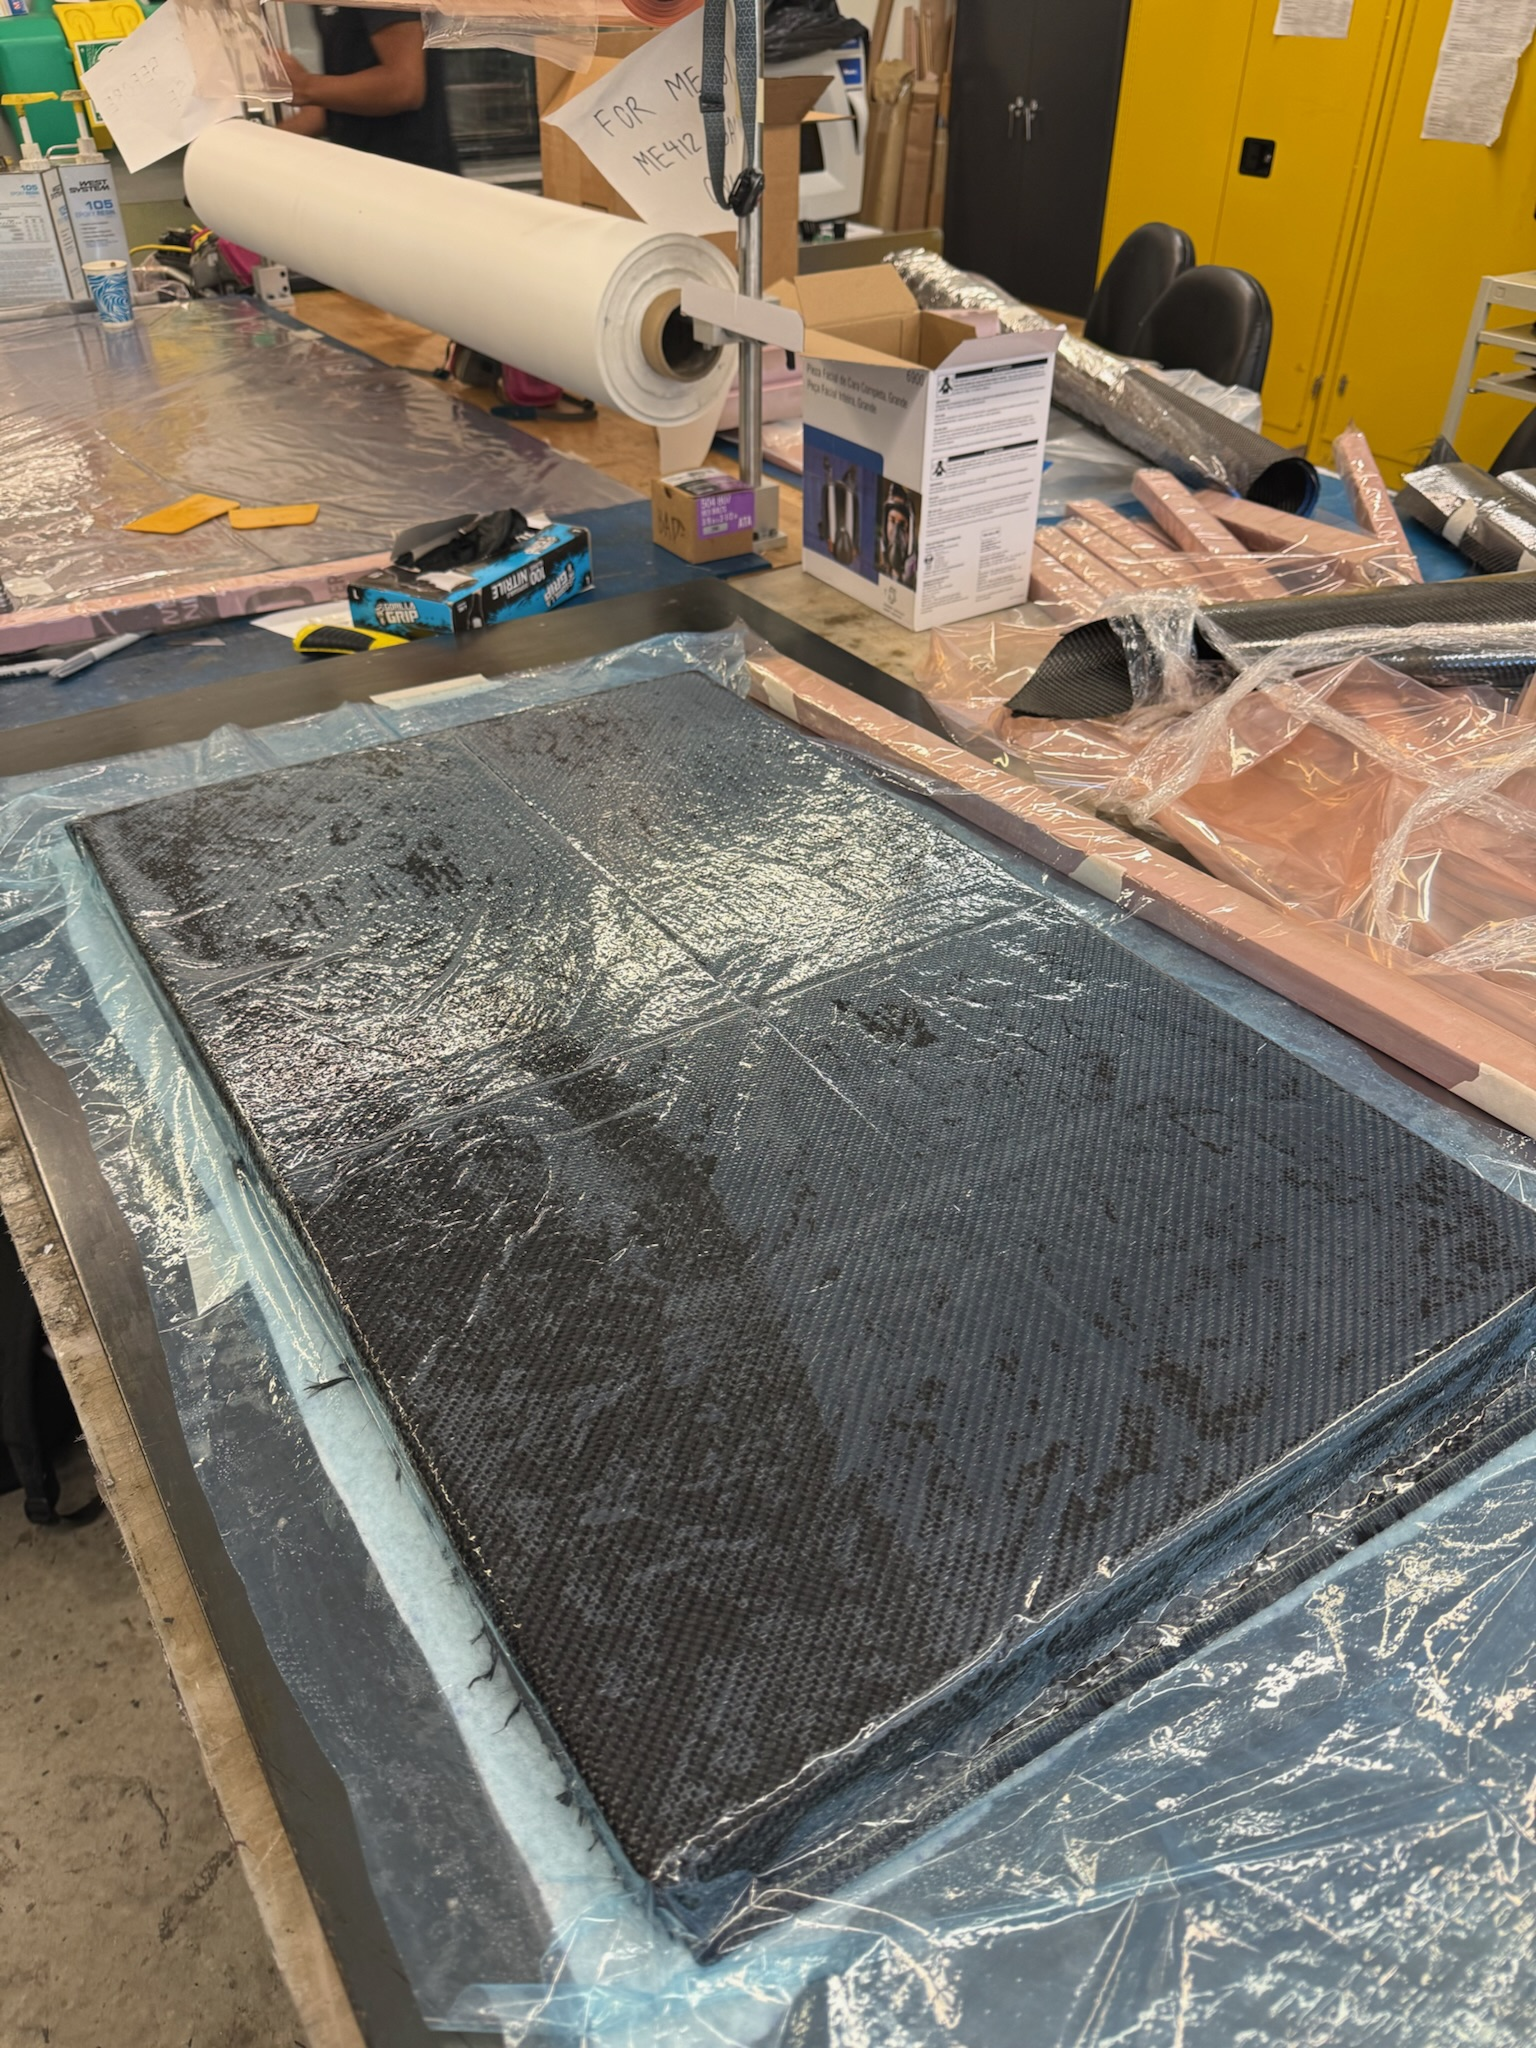
\includegraphics[
        width=3.10in,
        height=1.40in,
        keepaspectratio
    ]{blue_perforrated_film_layup}
};
\draw[RuleGray,line width=0.55pt,rounded corners=4pt]
    ($(current page.north west)+(7.29in,-3.36in)$)
    rectangle
    ($(current page.north east)+(-0.42in,-4.85in)$);

% Row 1 captions
\node[anchor=north,text=Muted,font=\sffamily\fontsize{6.7}{7.3}\selectfont]
at ($(current page.north west)+(2.07in,-4.90in)$)
{1. Waterjet-cut core and perimeter geometry};

\node[anchor=north,text=Muted,font=\sffamily\fontsize{6.7}{7.3}\selectfont]
at ($(current page.north west)+(5.50in,-4.90in)$)
{2. Team wet layup under my process guidance};

\node[anchor=north,text=Muted,font=\sffamily\fontsize{6.7}{7.3}\selectfont]
at ($(current page.north west)+(8.935in,-4.90in)$)
{3. Perforated film, breather, and vacuum enclosure};

% Row 2 image 1
\node[anchor=center,inner sep=0pt]
at ($(current page.north west)+(2.07in,-5.875in)$)
{
    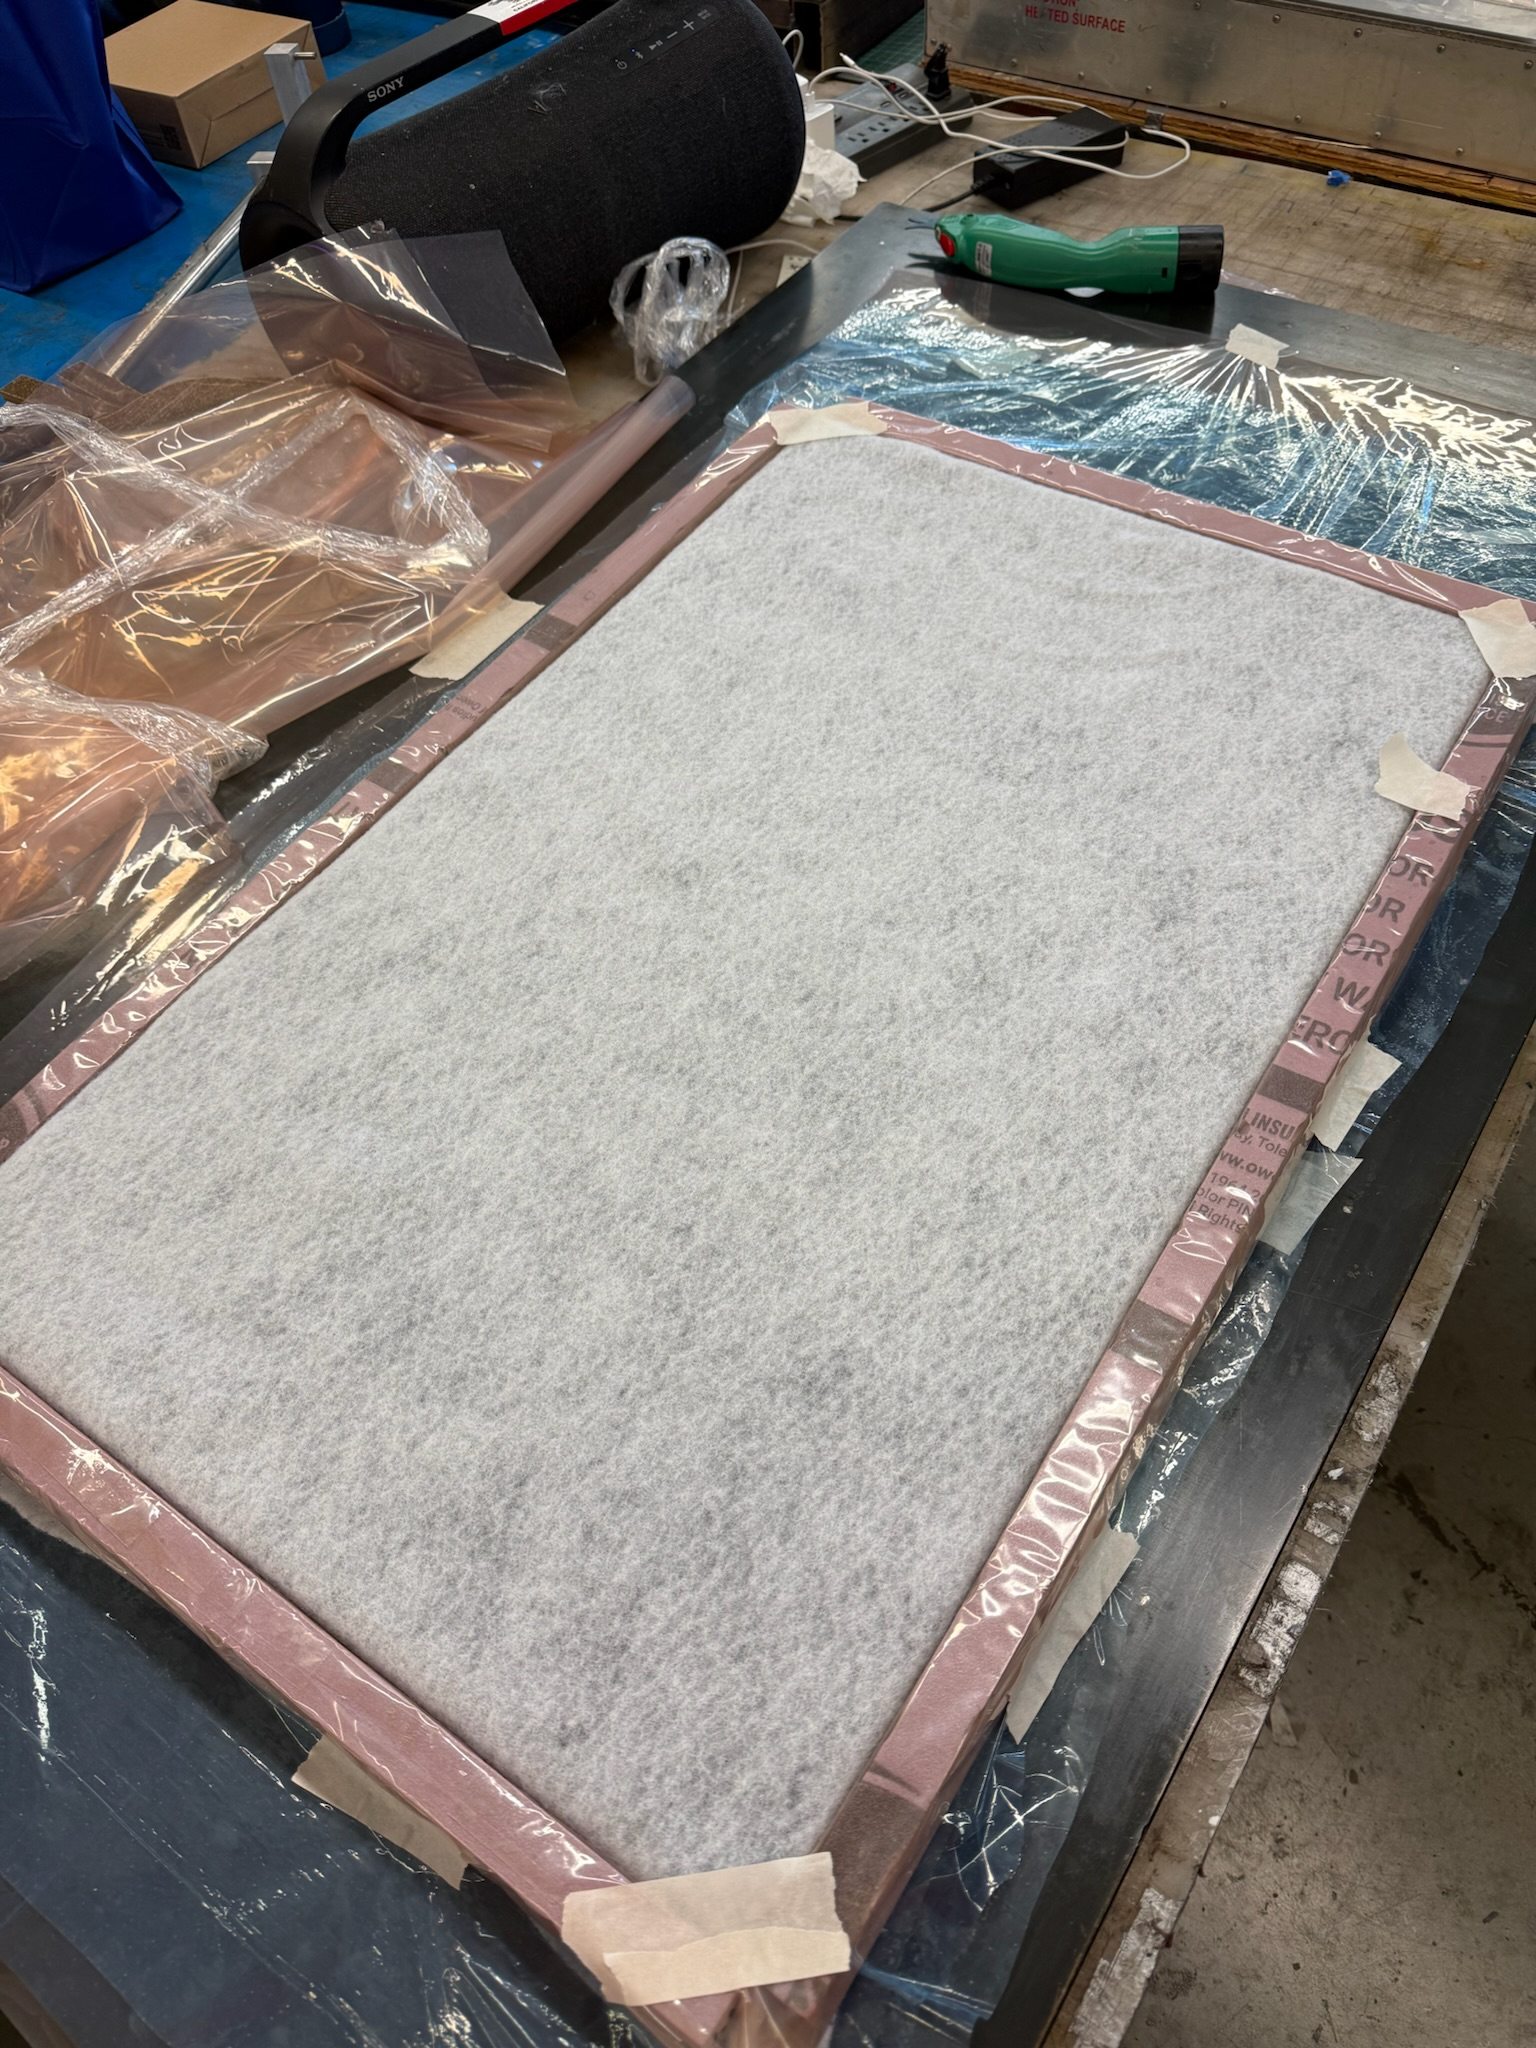
\includegraphics[
        width=3.10in,
        height=1.40in,
        keepaspectratio
    ]{completed_layup}
};
\draw[RuleGray,line width=0.55pt,rounded corners=4pt]
    ($(current page.north west)+(0.43in,-5.13in)$)
    rectangle
    ($(current page.north west)+(3.71in,-6.62in)$);

% Row 2 image 2 — oven chamber used only as a reliable vacuum enclosure; no heat applied
\node[anchor=center,inner sep=0pt]
at ($(current page.north west)+(5.50in,-5.875in)$)
{
    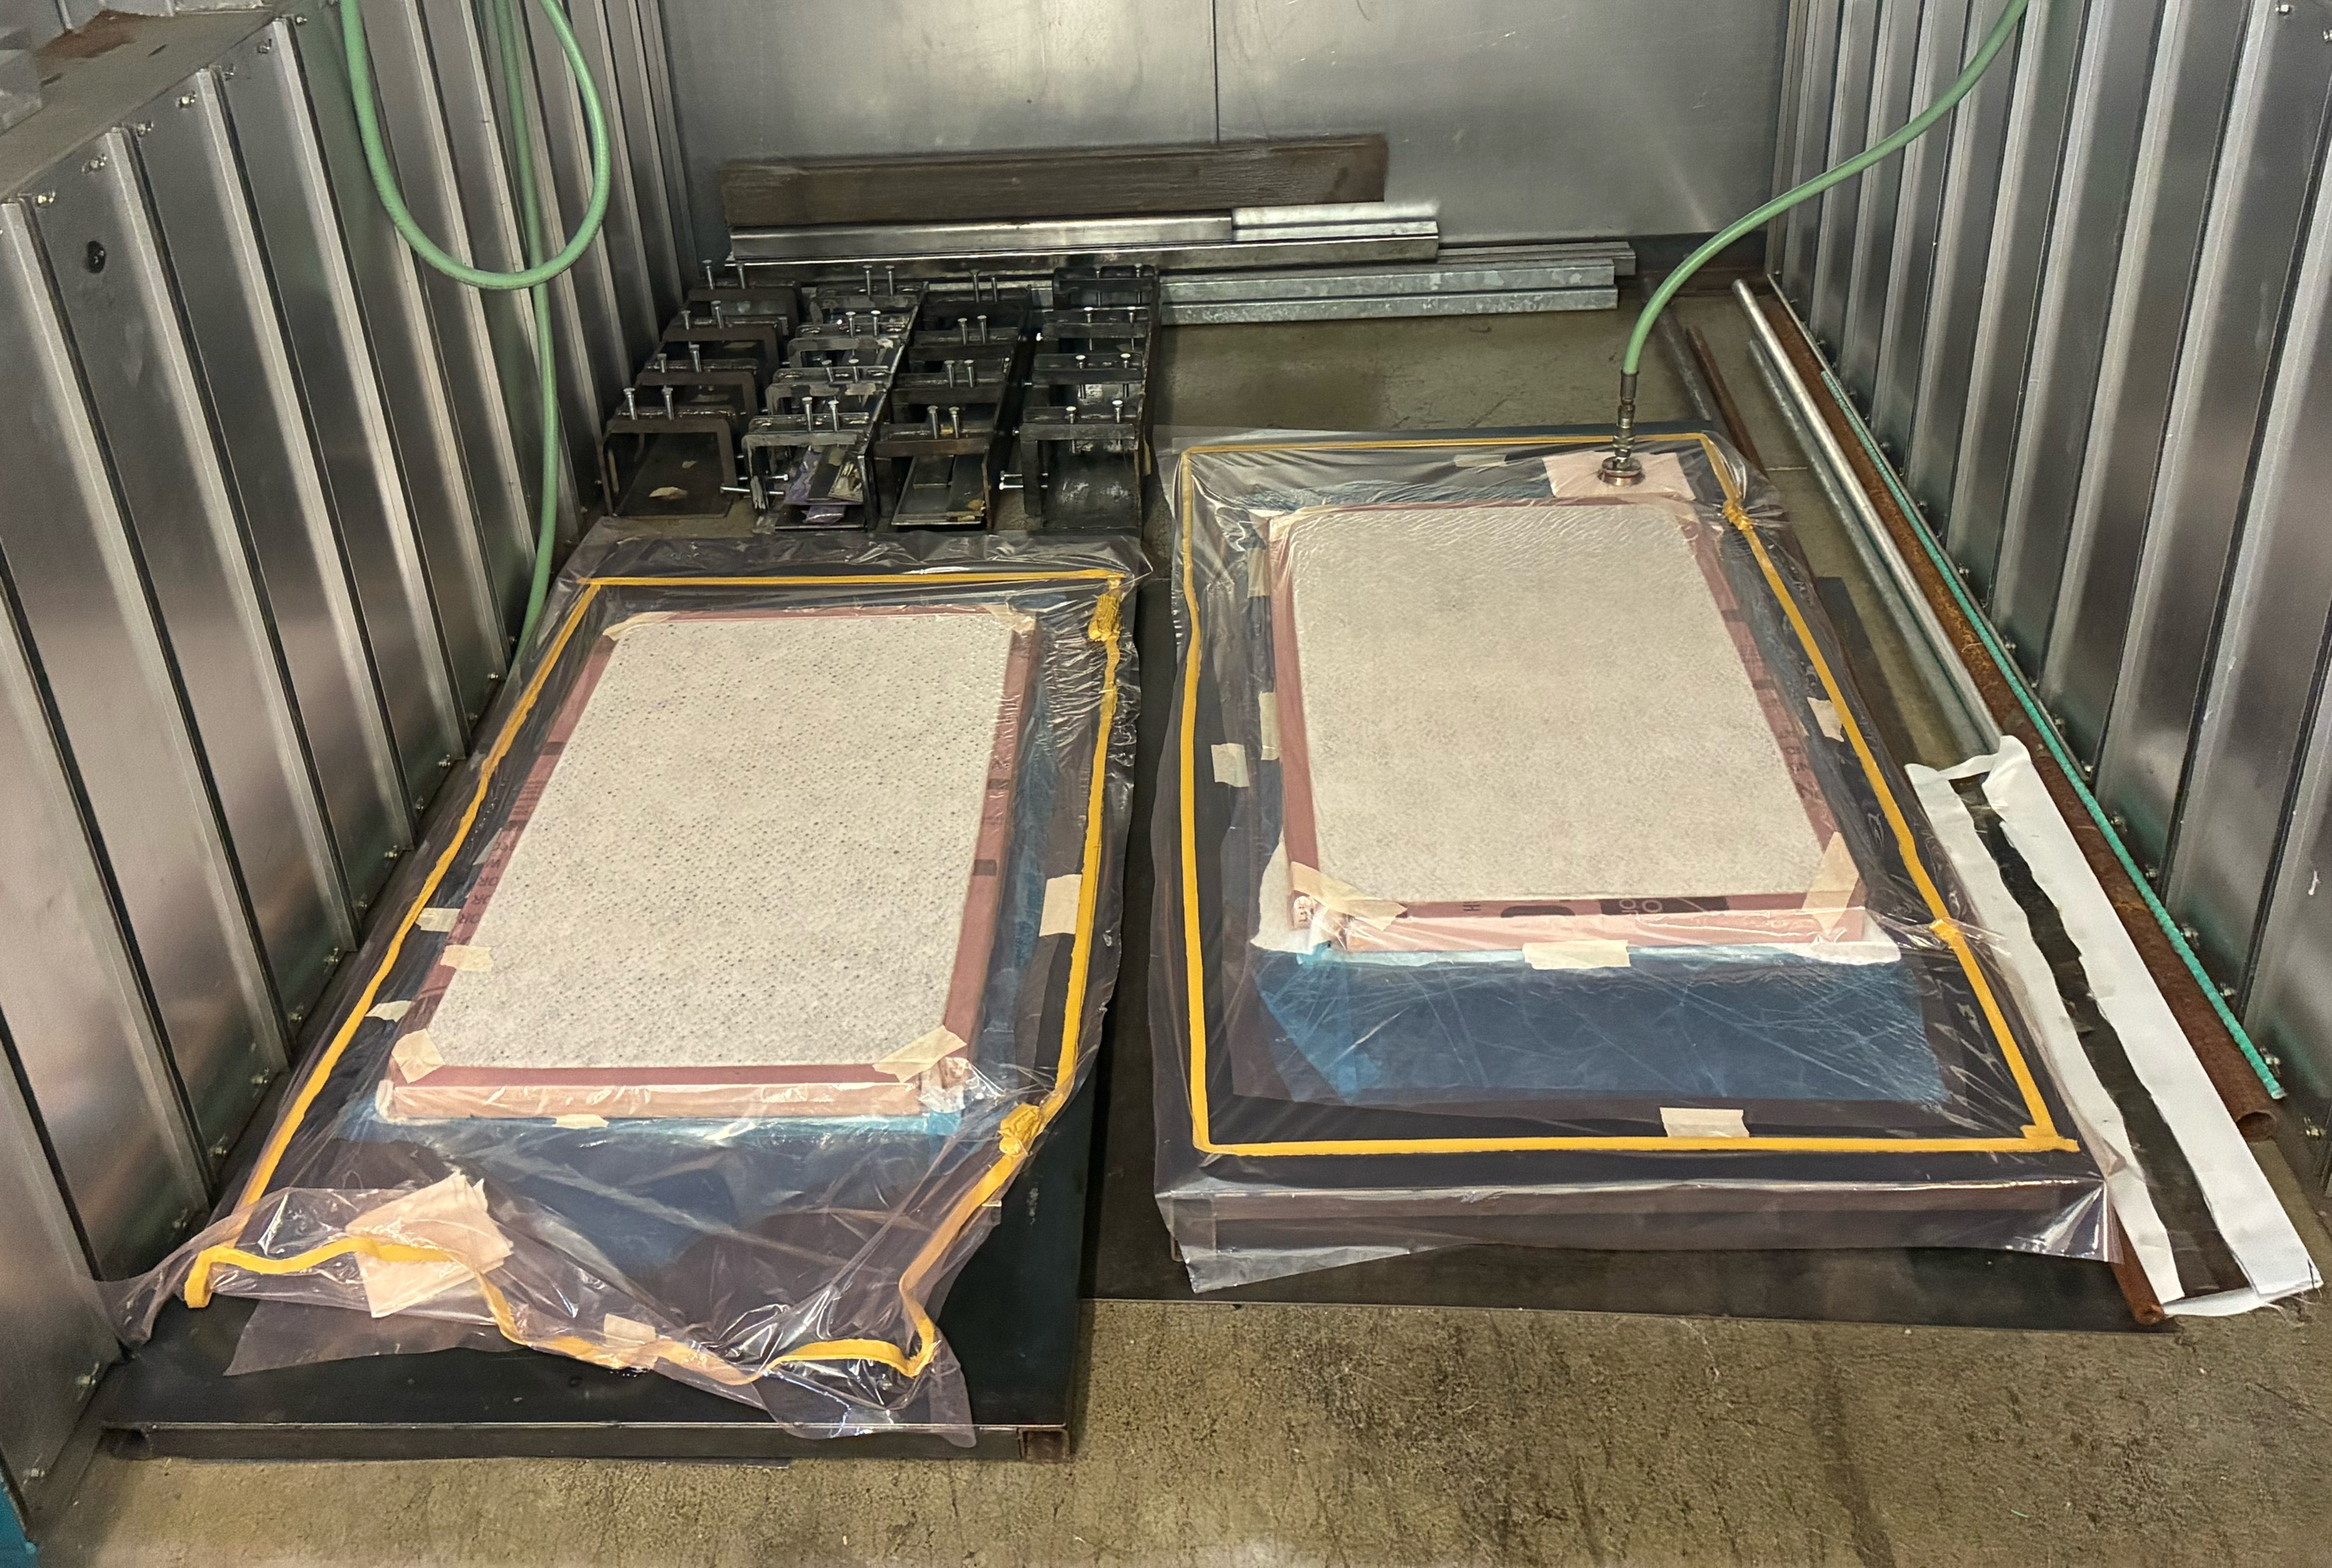
\includegraphics[
        width=3.10in,
        height=1.40in,
        keepaspectratio
    ]{layups_in_composite_oven_under_vacuumPressure}
};
\draw[RuleGray,line width=0.55pt,rounded corners=4pt]
    ($(current page.north west)+(3.86in,-5.13in)$)
    rectangle
    ($(current page.north west)+(7.14in,-6.62in)$);

% Row 2 image 3
\node[anchor=center,inner sep=0pt]
at ($(current page.north west)+(8.935in,-5.875in)$)
{
    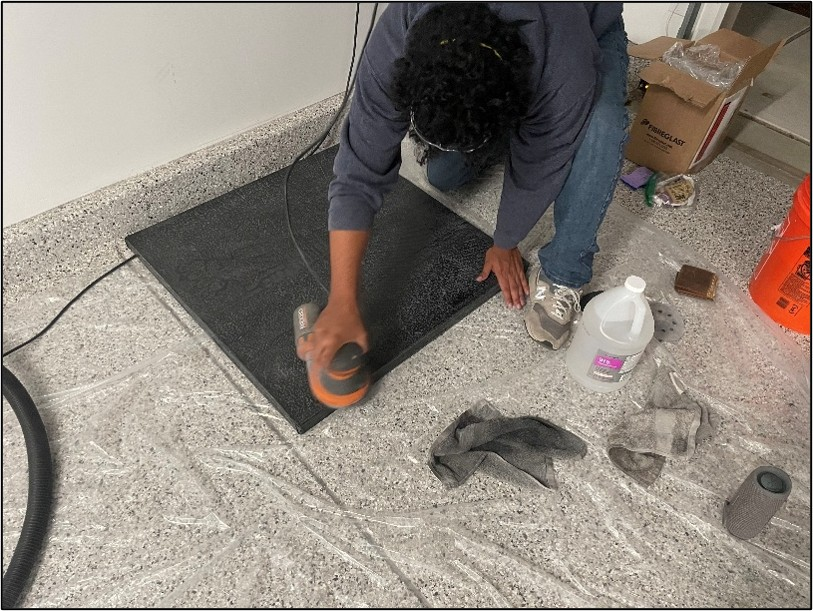
\includegraphics[
        width=3.10in,
        height=1.40in,
        keepaspectratio
    ]{garage_sanding}
};
\draw[RuleGray,line width=0.55pt,rounded corners=4pt]
    ($(current page.north west)+(7.29in,-5.13in)$)
    rectangle
    ($(current page.north east)+(-0.42in,-6.62in)$);

% Row 2 captions
\node[anchor=north,text=Muted,font=\sffamily\fontsize{6.7}{7.3}\selectfont]
at ($(current page.north west)+(2.07in,-6.67in)$)
{4. Fully saturated carbon skin and foam sandwich};

\node[anchor=north,text=Muted,font=\sffamily\fontsize{6.7}{7.3}\selectfont]
at ($(current page.north west)+(5.50in,-6.67in)$)
{5. Room-temperature cure under continuous vacuum};

\node[anchor=north,text=Muted,font=\sffamily\fontsize{6.7}{7.3}\selectfont]
at ($(current page.north west)+(8.935in,-6.67in)$)
{6. Post-processing and surface preparation};

% Bottom callouts
\fill[Panel,rounded corners=4pt]
    ($(current page.north west)+(0.43in,-6.95in)$)
    rectangle
    ($(current page.north west)+(5.48in,-7.60in)$);

\draw[RuleGray,line width=0.55pt,rounded corners=4pt]
    ($(current page.north west)+(0.43in,-6.95in)$)
    rectangle
    ($(current page.north west)+(5.48in,-7.60in)$);

\node[
    anchor=north west,
    text=DeepGreen,
    font=\sffamily\bfseries\fontsize{7.0}{7.6}\selectfont
]
at ($(current page.north west)+(0.63in,-7.08in)$)
{FROM THREE LAYUPS TO ONE};

\node[
    anchor=north west,
    align=left,
    text width=4.56in,
    text=Ink,
    font=\fontsize{6.45}{7.45}\selectfont
]
at ($(current page.north west)+(0.63in,-7.29in)$)
{
The Envelope Method reduced labor, cure cycles, handling,
alignment risk, and time spent forming numerous vacuum-bag
pleats around the 1.5-inch-thick XPS panels.
};

\fill[Panel,rounded corners=4pt]
    ($(current page.north west)+(5.68in,-6.95in)$)
    rectangle
    ($(current page.north east)+(-0.42in,-7.60in)$);

\draw[RuleGray,line width=0.55pt,rounded corners=4pt]
    ($(current page.north west)+(5.68in,-6.95in)$)
    rectangle
    ($(current page.north east)+(-0.42in,-7.60in)$);

\node[
    anchor=north west,
    text=DeepGreen,
    font=\sffamily\bfseries\fontsize{7.0}{7.6}\selectfont
]
at ($(current page.north west)+(5.88in,-7.08in)$)
{WHY SURFACE-BONDED HARDWARE};

\node[
    anchor=north west,
    align=left,
    text width=4.55in,
    text=Ink,
    font=\fontsize{6.45}{7.45}\selectfont
]
at ($(current page.north west)+(5.88in,-7.29in)$)
{
Adhesively bonded hinges and fixtures preserved the clean
composite exterior and avoided drilled inserts, foam-core
crushing, added stress concentrations, and new leak paths.
};


% Footer
\node[
    anchor=south west,
    text=white,
    font=\sffamily\bfseries\fontsize{7.1}{7.7}\selectfont
]
at ($(current page.south west)+(0.42in,0.17in)$)
{\faArrowLeft\ PRODUCT ARCHITECTURE};

\node[
    anchor=south,
    text=white,
    font=\sffamily\fontsize{7.0}{7.6}\selectfont
]
at ($(current page.south)+(0,0.17in)$)
{TORO COVER \hspace{6pt} 2 / 3};

\node[
    anchor=south east,
    text=white,
    font=\sffamily\bfseries\fontsize{7.1}{7.7}\selectfont
]
at ($(current page.south east)+(-0.42in,0.17in)$)
{VALIDATION \& TAKEAWAYS \faArrowRight};

\end{tikzpicture}


% ============================================================
% PAGE 3 — FINISHING, VALIDATION, AND TAKEAWAYS
% ============================================================

\clearpage
\thispagestyle{empty}
\hypertarget{toro-results}{}
\null

\begin{tikzpicture}[remember picture,overlay]

% Background and bars
\fill[white]
    (current page.south west)
    rectangle
    (current page.north east);

\fill[DeepGreen]
    (current page.north west)
    rectangle
    ($(current page.north east)+(0,-0.095in)$);

\fill[PolyGold]
    ($(current page.north west)+(0,-0.095in)$)
    rectangle
    ($(current page.north east)+(0,-0.14in)$);

\fill[DeepGreen]
    (current page.south west)
    rectangle
    ($(current page.south east)+(0,0.36in)$);

\fill[PolyGold]
    ($(current page.south west)+(0,0.36in)$)
    rectangle
    ($(current page.south east)+(0,0.405in)$);

% Header
\node[
    anchor=north west,
    text=PolyGold,
    font=\sffamily\bfseries\fontsize{8.1}{8.7}\selectfont
]
at ($(current page.north west)+(0.42in,-0.39in)$)
{TORO COVER \hspace{5pt}/\hspace{5pt} VALIDATION AND ENGINEERING TAKEAWAYS};

\node[
    anchor=north west,
    text=DeepGreen,
    font=\bfseries\fontsize{22.5}{23.5}\selectfont
]
at ($(current page.north west)+(0.40in,-0.67in)$)
{FROM PROTOTYPE TO PRODUCT PATHWAY};

\node[
    anchor=north west,
    text=Muted,
    font=\sffamily\fontsize{8.7}{9.6}\selectfont
]
at ($(current page.north west)+(0.42in,-1.12in)$)
{Environmental protection, usability testing, scope decisions, and lessons from technical leadership};

\fill[PolyGold]
    ($(current page.north west)+(0.42in,-1.36in)$)
    rectangle
    ($(current page.north west)+(5.8in,-1.315in)$);

% Finishing title
\node[
    anchor=north west,
    text=DeepGreen,
    font=\sffamily\bfseries\fontsize{8.0}{8.7}\selectfont
]
at ($(current page.north west)+(0.43in,-1.62in)$)
{OUTDOOR FINISHING AND ENVIRONMENTAL PROTECTION};

% Image 1
\node[anchor=center,inner sep=0pt]
at ($(current page.north west)+(1.705in,-2.655in)$)
{
    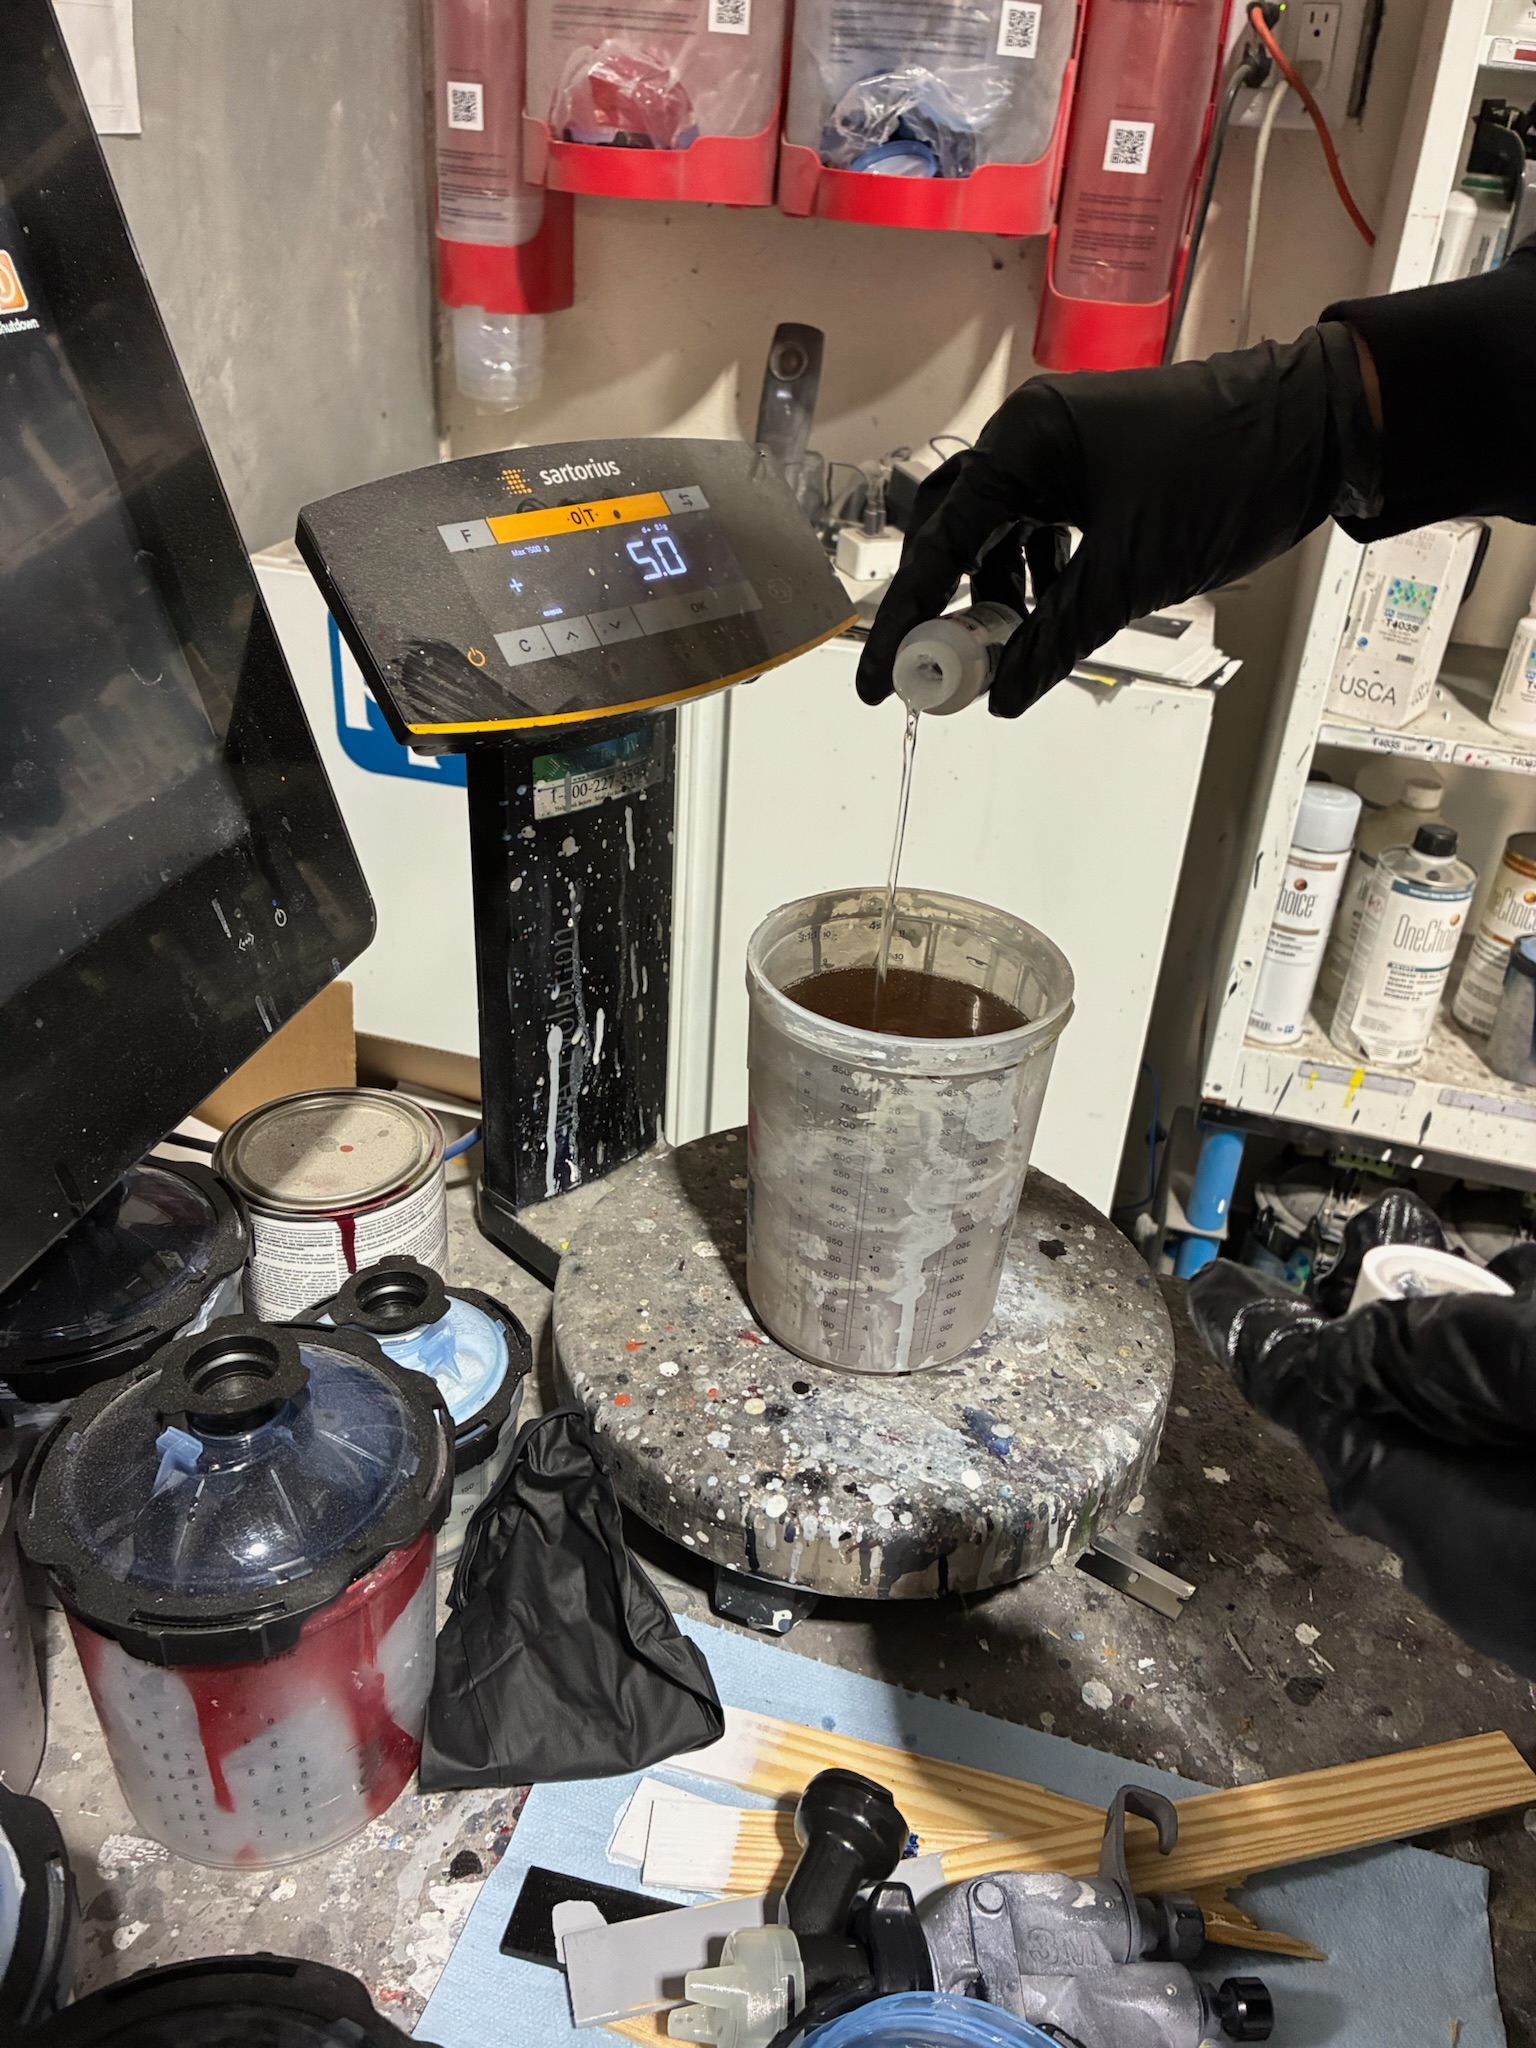
\includegraphics[
        width=2.35in,
        height=1.40in,
        keepaspectratio
    ]{spray_topcoat_prep}
};
\draw[RuleGray,line width=0.55pt,rounded corners=4pt]
    ($(current page.north west)+(0.43in,-1.91in)$)
    rectangle
    ($(current page.north west)+(2.98in,-3.40in)$);

% Image 2
\node[anchor=center,inner sep=0pt]
at ($(current page.north west)+(4.375in,-2.655in)$)
{
    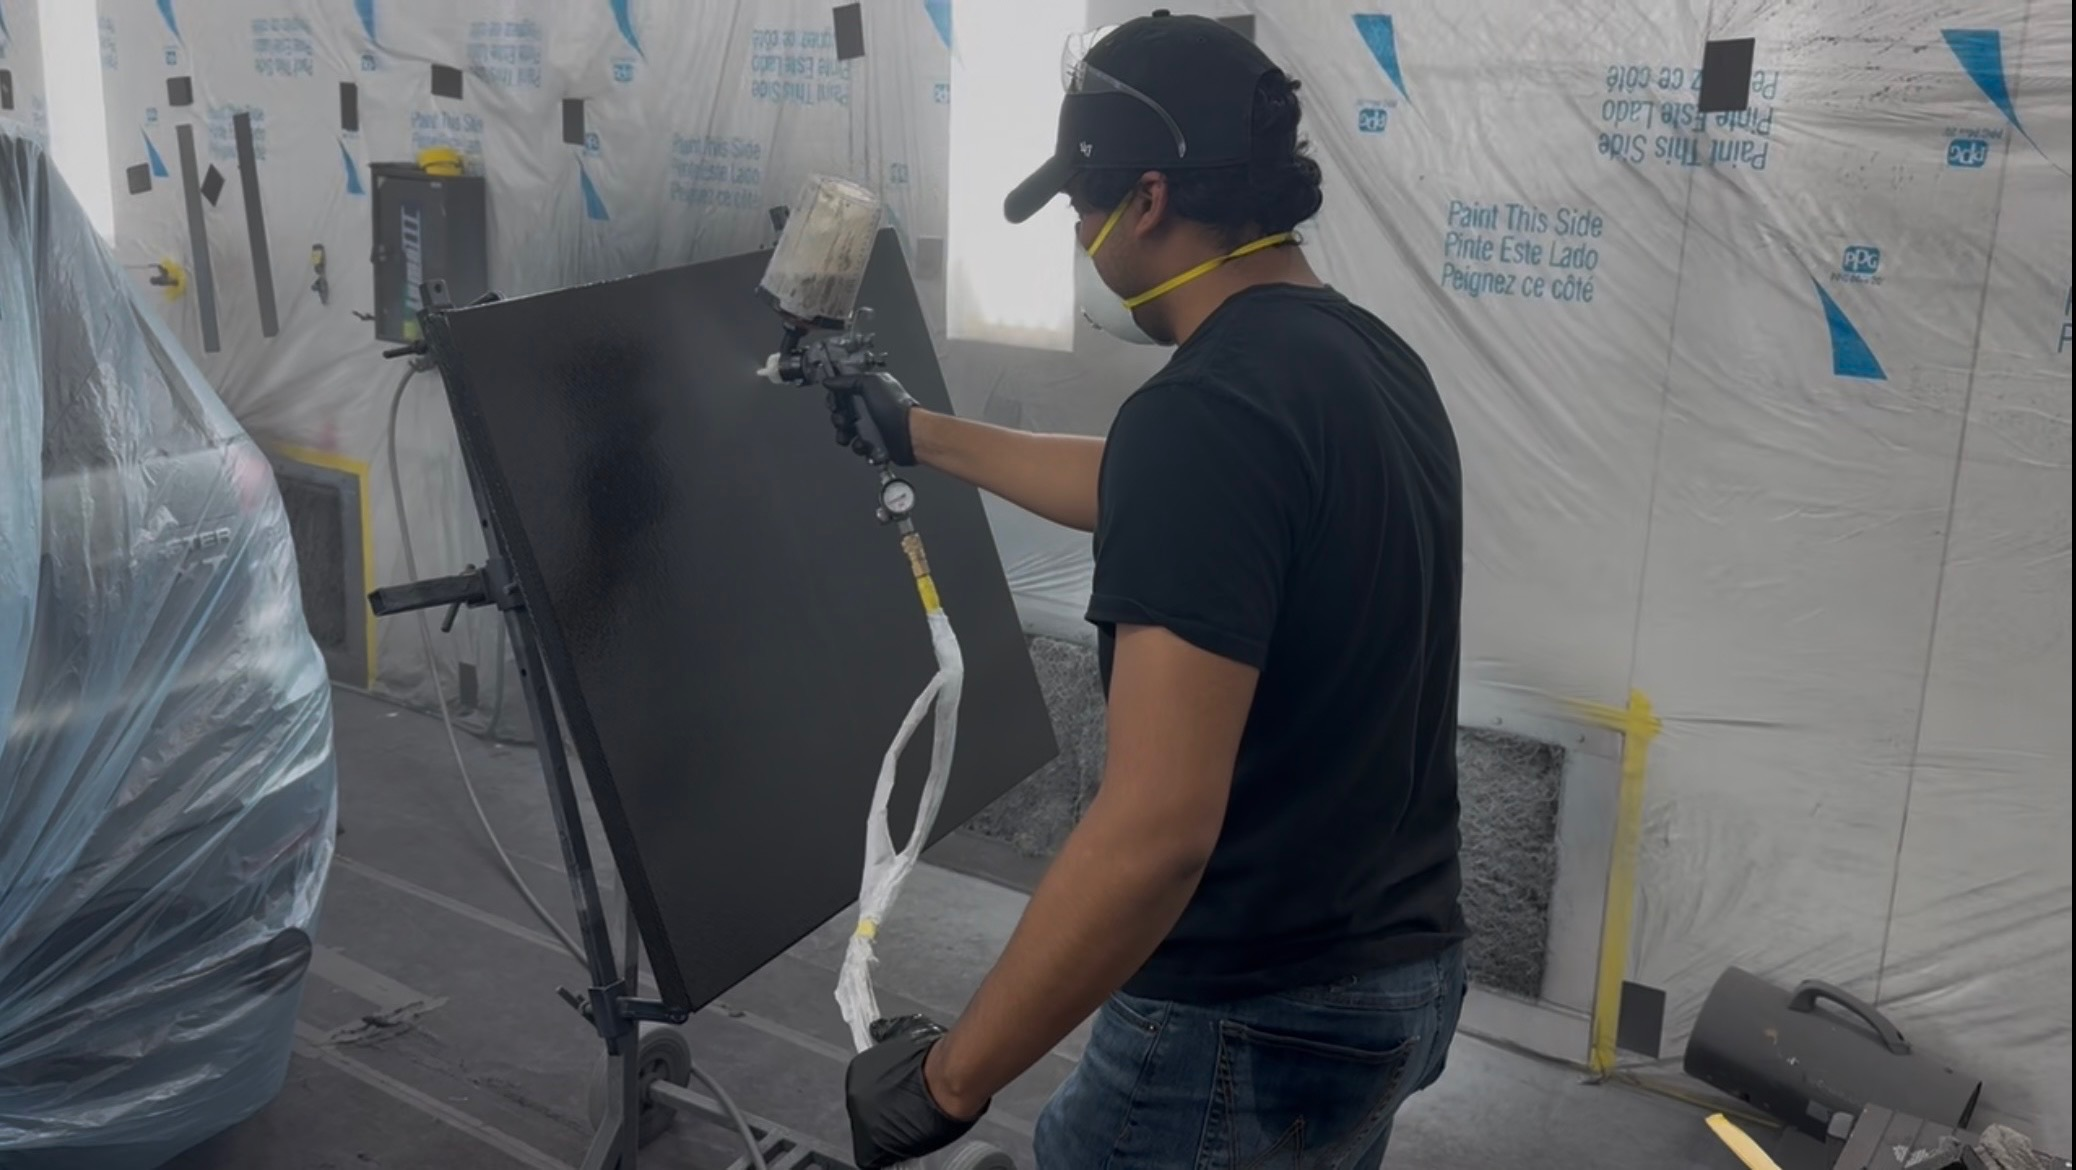
\includegraphics[
        width=2.35in,
        height=1.40in,
        keepaspectratio
    ]{spraying_topcoat}
};
\draw[RuleGray,line width=0.55pt,rounded corners=4pt]
    ($(current page.north west)+(3.10in,-1.91in)$)
    rectangle
    ($(current page.north west)+(5.65in,-3.40in)$);

% Image 3
\node[anchor=center,inner sep=0pt]
at ($(current page.north west)+(7.045in,-2.655in)$)
{
    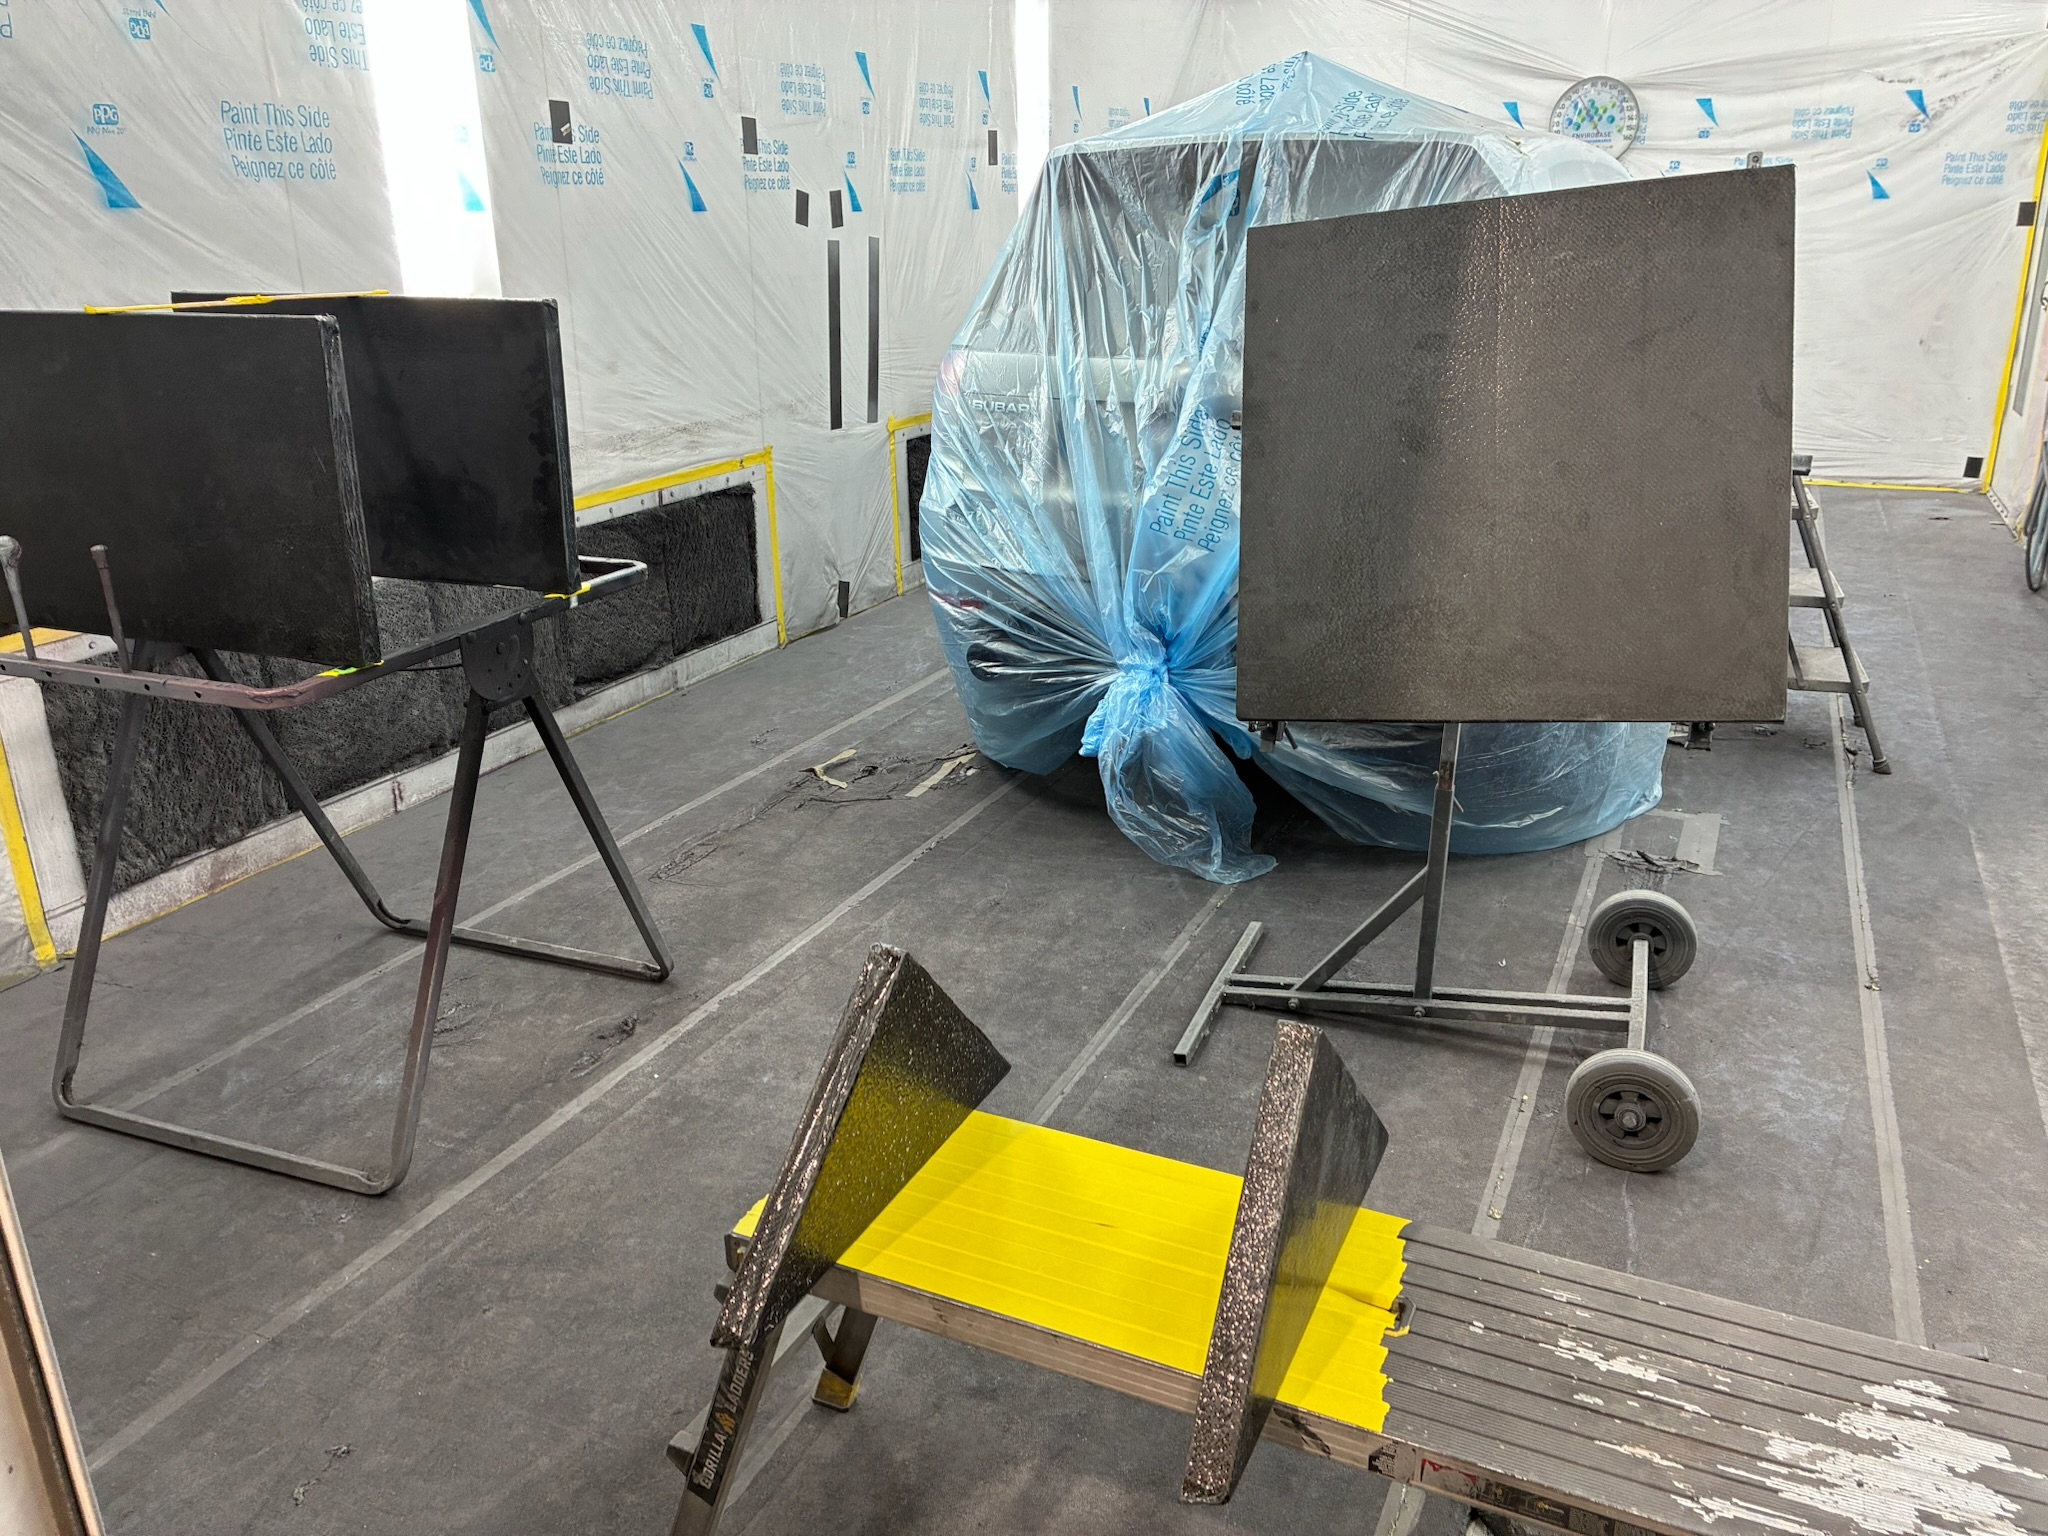
\includegraphics[
        width=2.35in,
        height=1.40in,
        keepaspectratio
    ]{topcoat_setup_apparatus}
};
\draw[RuleGray,line width=0.55pt,rounded corners=4pt]
    ($(current page.north west)+(5.77in,-1.91in)$)
    rectangle
    ($(current page.north west)+(8.32in,-3.40in)$);

% Image 4
\node[anchor=center,inner sep=0pt]
at ($(current page.north west)+(9.50in,-2.655in)$)
{
    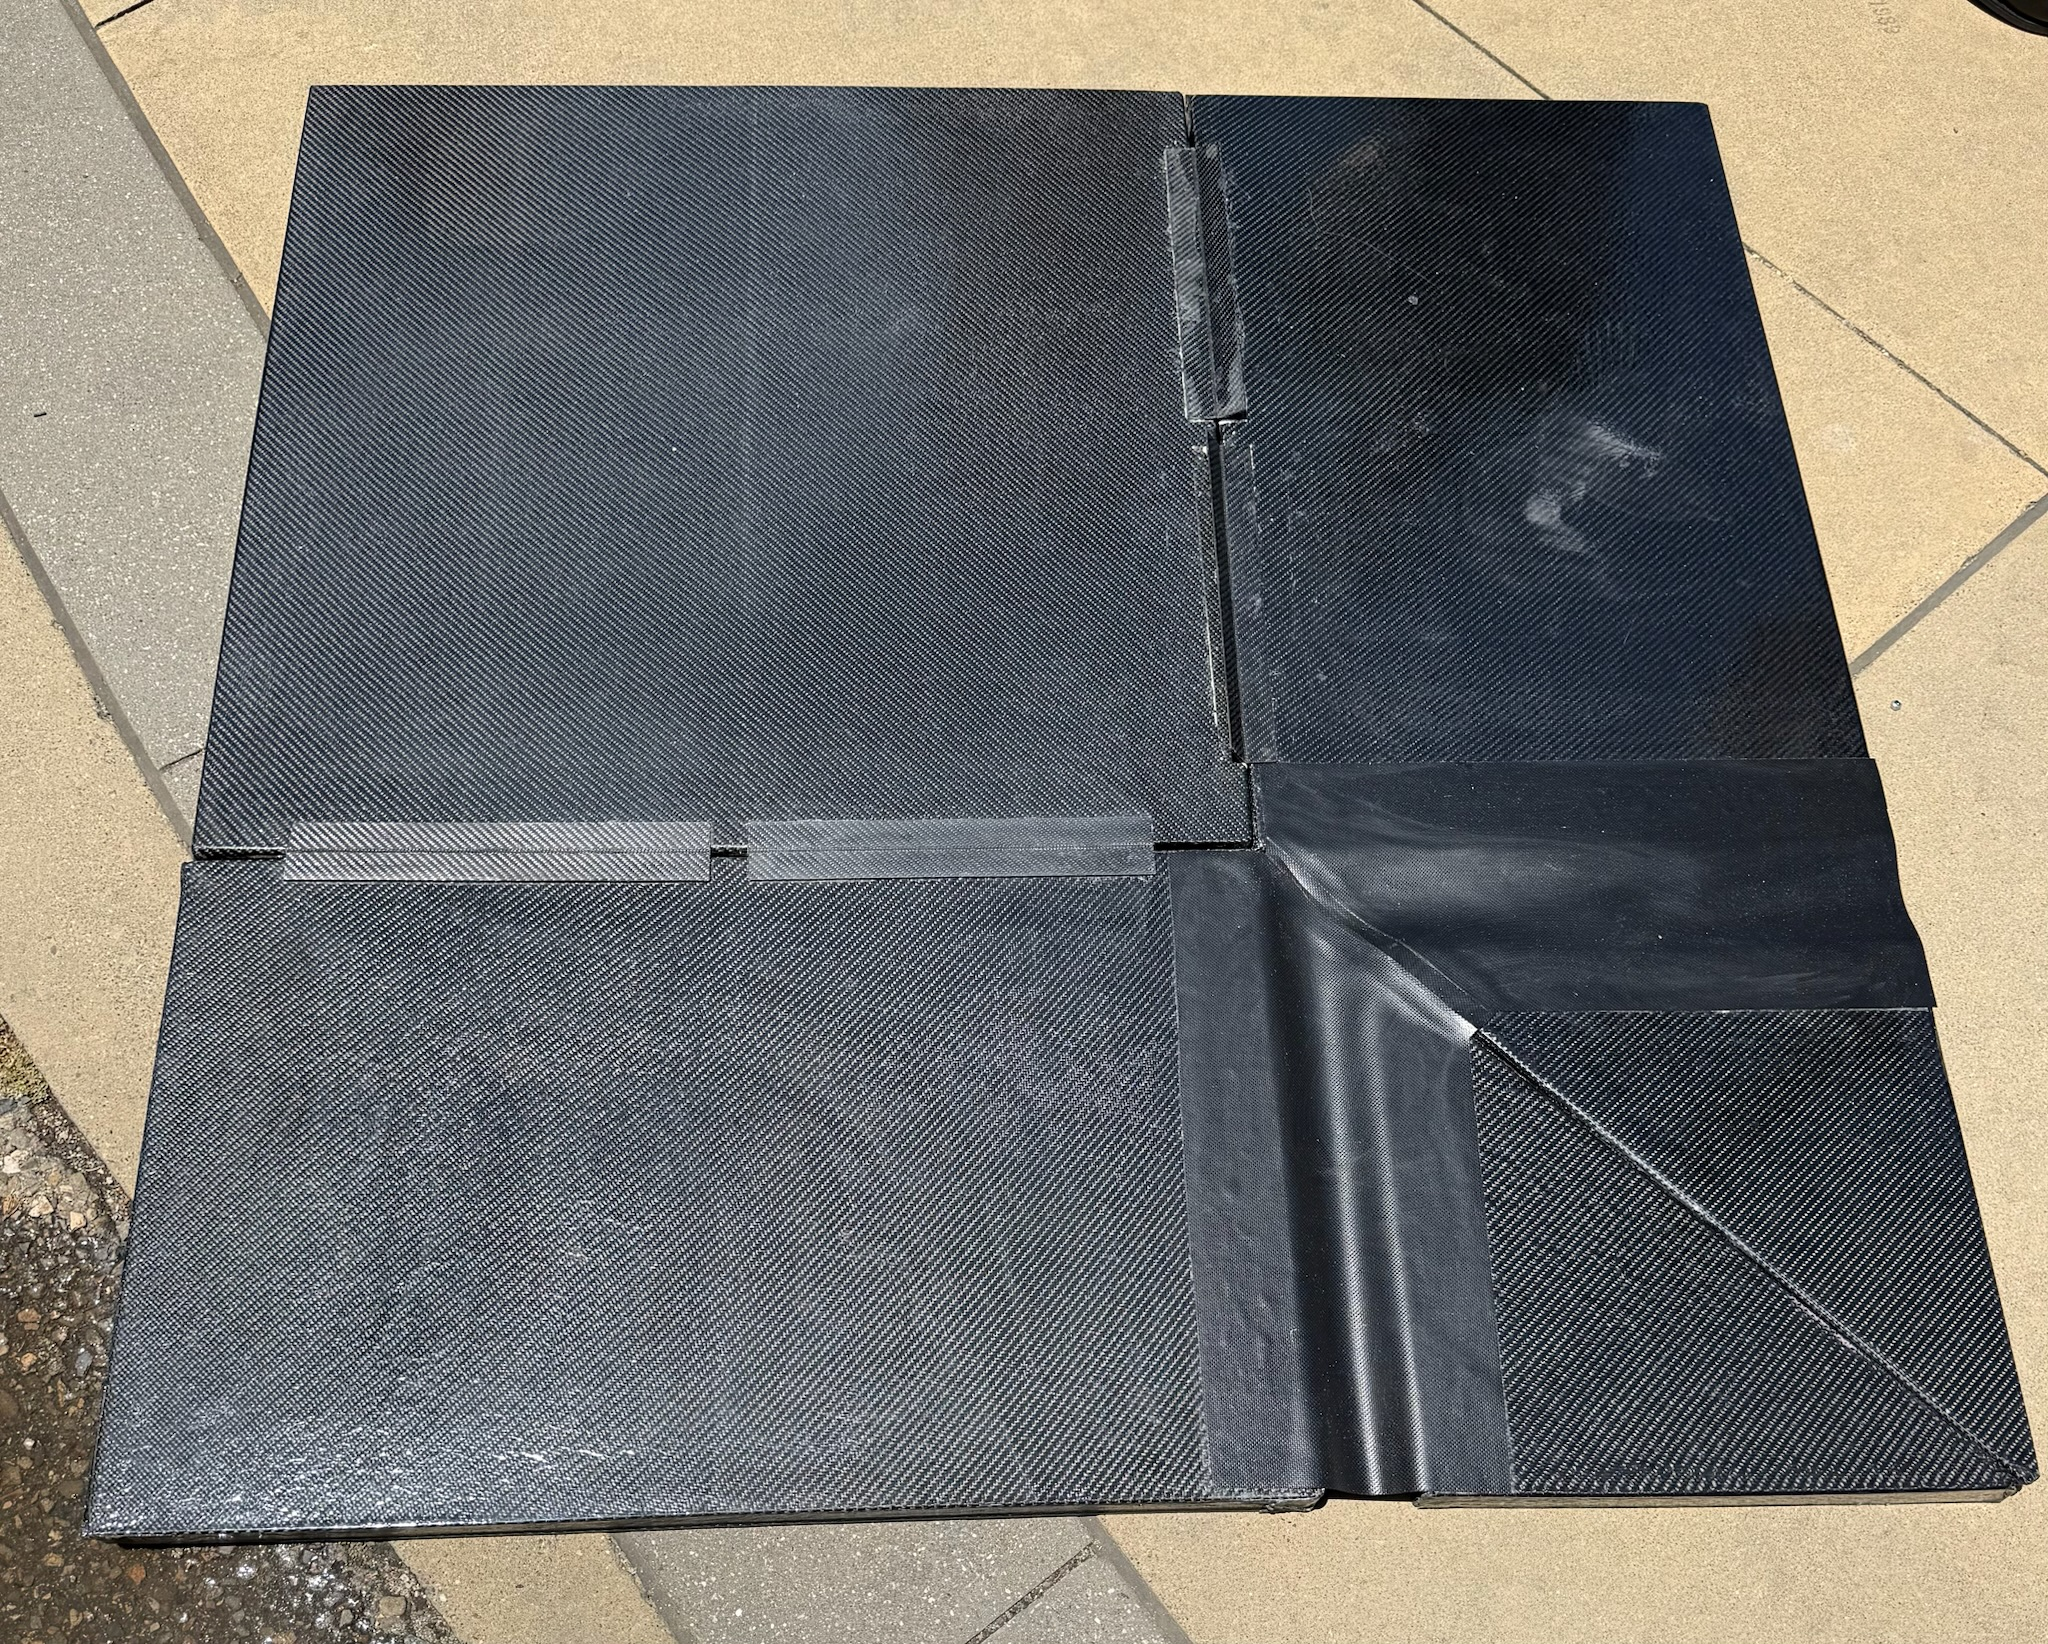
\includegraphics[
        width=2.35in,
        height=1.40in,
        keepaspectratio
    ]{refined_final_toro_cover_partial_carbon_model}
};
\draw[RuleGray,line width=0.55pt,rounded corners=4pt]
    ($(current page.north west)+(8.44in,-1.91in)$)
    rectangle
    ($(current page.north east)+(-0.42in,-3.40in)$);

% Captions
\node[anchor=north,text=Muted,font=\sffamily\fontsize{6.7}{7.3}\selectfont]
at ($(current page.north west)+(1.705in,-3.45in)$)
{Topcoat material preparation};

\node[anchor=north,text=Muted,font=\sffamily\fontsize{6.7}{7.3}\selectfont]
at ($(current page.north west)+(4.375in,-3.45in)$)
{Automotive-booth topcoat application};

\node[anchor=north,text=Muted,font=\sffamily\fontsize{6.7}{7.3}\selectfont]
at ($(current page.north west)+(7.045in,-3.45in)$)
{Coated panels drying after application};

\node[anchor=north,text=Muted,font=\sffamily\fontsize{6.7}{7.3}\selectfont]
at ($(current page.north west)+(9.50in,-3.45in)$)
{Partial carbon manufacturing model};

% Environmental rationale
\fill[SoftGold,rounded corners=4pt]
    ($(current page.north west)+(0.43in,-3.73in)$)
    rectangle
    ($(current page.north east)+(-0.42in,-4.76in)$);

\node[
    anchor=north west,
    align=left,
    text width=9.75in,
    text=Ink,
    font=\fontsize{7.05}{8.25}\selectfont
]
at ($(current page.north west)+(0.65in,-3.89in)$)
{
Because the sponsor required a carbon-fiber cover for outdoor use near chlorinated water,
environmental protection became a functional requirement rather than a cosmetic finish.
I selected and personally sprayed a UV-resistant Sunshield topcoat to seal minor laminate
porosity, reduce moisture ingress, preserve the carbon appearance, limit UV degradation of
the epoxy matrix, and isolate the composite surface from nearby metallic hardware.
};

% Results title
\node[
    anchor=north west,
    text=DeepGreen,
    font=\sffamily\bfseries\fontsize{8.0}{8.7}\selectfont
]
at ($(current page.north west)+(0.43in,-4.94in)$)
{FUNCTIONAL PROTOTYPE RESULTS};

% ------------------------------------------------------------
% Matched lower panels — larger type and improved allocation
% ------------------------------------------------------------

% Left results panel
\fill[SoftGreen,rounded corners=5pt]
    ($(current page.north west)+(0.43in,-5.22in)$)
    rectangle
    ($(current page.north west)+(5.98in,-7.39in)$);

\draw[RuleGray,line width=0.65pt,rounded corners=5pt]
    ($(current page.north west)+(0.43in,-5.22in)$)
    rectangle
    ($(current page.north west)+(5.98in,-7.39in)$);

\fill[DeepGreen,rounded corners=5pt]
    ($(current page.north west)+(0.43in,-5.22in)$)
    rectangle
    ($(current page.north west)+(5.98in,-5.58in)$);

\fill[DeepGreen]
    ($(current page.north west)+(0.43in,-5.40in)$)
    rectangle
    ($(current page.north west)+(5.98in,-5.58in)$);

\node[anchor=west,text=white,
      font=\sffamily\bfseries\fontsize{7.0}{7.6}\selectfont]
at ($(current page.north west)+(0.66in,-5.40in)$)
{SPECIFICATION};

\node[anchor=west,text=white,
      font=\sffamily\bfseries\fontsize{7.0}{7.6}\selectfont]
at ($(current page.north west)+(3.02in,-5.40in)$)
{RESULT};

\node[anchor=east,text=white,
      font=\sffamily\bfseries\fontsize{7.0}{7.6}\selectfont]
at ($(current page.north west)+(5.55in,-5.40in)$)
{STATUS};

\node[
    anchor=north west,
    align=left,
    text width=2.15in,
    text=Ink,
    font=\bfseries\fontsize{7.15}{8.55}\selectfont
]
at ($(current page.north west)+(0.66in,-5.72in)$)
{
Deployment time\\[3.4pt]
Removal time\\[3.4pt]
Single-user operation\\[3.4pt]
Single-side operation\\[3.4pt]
Deployment steps\\[3.4pt]
Removal steps\\[3.4pt]
Weight\\[3.4pt]
Folded storage
};

\node[
    anchor=north west,
    align=left,
    text width=1.45in,
    text=Ink,
    font=\fontsize{7.15}{8.55}\selectfont
]
at ($(current page.north west)+(3.02in,-5.72in)$)
{
25.51 seconds\\[3.4pt]
37.22 seconds\\[3.4pt]
100\% successful\\[3.4pt]
75\% successful\\[3.4pt]
6.4 average\\[3.4pt]
9 average\\[3.4pt]
17 lb\\[3.4pt]
2.9' x 2.9' x 1.7'
};

\node[
    anchor=north east,
    align=right,
    text width=1.05in,
    text=DeepGreen,
    font=\sffamily\bfseries\fontsize{7.05}{8.55}\selectfont
]
at ($(current page.north west)+(5.55in,-5.72in)$)
{
PASS\\[3.4pt]
PASS\\[3.4pt]
PASS\\[3.4pt]
NEAR TARGET\\[3.4pt]
PASS\\[3.4pt]
PASS\\[3.4pt]
NEAR TARGET\\[3.4pt]
PASS
};

% Right takeaways panel — widened for easier reading
\fill[SoftGreen,rounded corners=5pt]
    ($(current page.north west)+(6.14in,-5.22in)$)
    rectangle
    ($(current page.north east)+(-0.42in,-7.39in)$);

\draw[RuleGray,line width=0.65pt,rounded corners=5pt]
    ($(current page.north west)+(6.14in,-5.22in)$)
    rectangle
    ($(current page.north east)+(-0.42in,-7.39in)$);

\fill[DeepGreen,rounded corners=5pt]
    ($(current page.north west)+(6.14in,-5.22in)$)
    rectangle
    ($(current page.north east)+(-0.42in,-5.58in)$);

\fill[DeepGreen]
    ($(current page.north west)+(6.14in,-5.40in)$)
    rectangle
    ($(current page.north east)+(-0.42in,-5.58in)$);

\node[anchor=west,text=white,
      font=\sffamily\bfseries\fontsize{7.1}{7.7}\selectfont]
at ($(current page.north west)+(6.38in,-5.40in)$)
{ENGINEERING TAKEAWAYS};

\node[
    anchor=north west,
    align=left,
    text width=4.02in,
    text=Ink,
    font=\fontsize{6.75}{7.85}\selectfont
]
at ($(current page.north west)+(6.38in,-5.72in)$)
{
\textbf{Manufacturing first.}
Composite manufacturing constraints should guide the product architecture from the beginning.\\[4.5pt]
\textbf{Prioritize deliberately.}
Competing requirements must be balanced intentionally instead of maximizing every objective.\\[4.5pt]
\textbf{Lead through the process.}
Clear procedures, calm communication, and respect for teammates' strengths were essential during fabrication.\\[4.5pt]
\textbf{Next iteration.}
Reduce weight, refine the fabric-hinge fold lines, and improve panel-edge clearance.
};

% Compact concluding pathway
\node[
    anchor=center,
    align=center,
    text=PolyGold,
    font=\sffamily\bfseries\fontsize{6.3}{6.9}\selectfont
]
at ($(current page.north)+(3.06in,-7.18in)$)
{PROTOTYPE \faArrowRight\ DESIGN REFINEMENT
\faArrowRight\ REPEATABLE MANUFACTURING
\faArrowRight\ PRODUCT};

% Validation resources
\node[
    anchor=north,
    align=center,
    text=DeepGreen,
    font=\sffamily\bfseries\fontsize{6.6}{7.2}\selectfont
]
at ($(current page.north)+(0,-7.58in)$)
{\href{\ToroDeploymentLink}{\faPlayCircle\ DEPLOYMENT}
\hspace{18pt}
\href{\ToroRemovalLink}{\faPlayCircle\ REMOVAL / FOLDING}
\hspace{18pt}
\href{\ToroPosterLink}{\faFilePdf\ EXPO POSTER}
\hspace{18pt}
\href{\ToroReportLink}{\faFilePdf\ FINAL REPORT}};

% Footer
\node[
    anchor=south west,
    text=white,
    font=\sffamily\bfseries\fontsize{7.1}{7.7}\selectfont
]
at ($(current page.south west)+(0.42in,0.17in)$)
{\faArrowLeft\ MANUFACTURING-DRIVEN DESIGN};

\node[
    anchor=south,
    text=white,
    font=\sffamily\fontsize{7.0}{7.6}\selectfont
]
at ($(current page.south)+(0,0.17in)$)
{TORO COVER \hspace{6pt} 3 / 3};

\node[
    anchor=south east,
    text=white,
    font=\sffamily\bfseries\fontsize{7.1}{7.7}\selectfont
]
at ($(current page.south east)+(-0.42in,0.17in)$)
{NEXT PROJECT \faArrowRight};

\end{tikzpicture}

% ============================================================
% PICKLEBALL PADDLE — SINGLE-PAGE PORTFOLIO CASE STUDY
% Project 02 in the Composites section
%
% IMPORTANT:
% 1. This file must NOT contain \documentclass, \begin{document},
%    or \end{document}.
% 2. In main.tex, place \input{pickleball} before \end{document}.
% 3. Image references use these Overleaf base filenames:
%       waterjet
%       side_core_view
%       full_assy
%       front_view
%       LAMINATE
% ============================================================

% Clickable project resource
\providecommand{\PaddleWaterjetVideo}
{https://drive.google.com/file/d/1mTuaE_g5mE2f7Nn3R5k7yFxqCWH_pvBh/view?usp=drive_link}

\clearpage
\thispagestyle{empty}
\hypertarget{pickleball}{}
\null

\begin{tikzpicture}[remember picture,overlay]

% ============================================================
% BACKGROUND AND PAGE BARS
% ============================================================

\fill[white]
    (current page.south west)
    rectangle
    (current page.north east);

\fill[DeepGreen]
    (current page.north west)
    rectangle
    ($(current page.north east)+(0,-0.095in)$);

\fill[PolyGold]
    ($(current page.north west)+(0,-0.095in)$)
    rectangle
    ($(current page.north east)+(0,-0.14in)$);

\fill[DeepGreen]
    (current page.south west)
    rectangle
    ($(current page.south east)+(0,0.36in)$);

\fill[PolyGold]
    ($(current page.south west)+(0,0.36in)$)
    rectangle
    ($(current page.south east)+(0,0.405in)$);

% ============================================================
% HEADER
% ============================================================

\node[
    anchor=north west,
    text=PolyGold,
    font=\sffamily\bfseries\fontsize{8.1}{8.7}\selectfont
]
at ($(current page.north west)+(0.42in,-0.39in)$)
{01 COMPOSITES \hspace{5pt}/\hspace{5pt} PROJECT 02};

\node[
    anchor=north west,
    text=DeepGreen,
    font=\bfseries\fontsize{22.5}{23.5}\selectfont
]
at ($(current page.north west)+(0.40in,-0.67in)$)
{CARBON FIBER PICKLEBALL PADDLE};

\node[
    anchor=north west,
    text=Muted,
    font=\sffamily\fontsize{8.4}{9.2}\selectfont
]
at ($(current page.north west)+(0.42in,-1.12in)$)
{Cal Poly Composites Laboratory \hspace{7pt}\textbullet\hspace{7pt}
Individual Project \hspace{7pt}\textbullet\hspace{7pt}
Spring 2026 \hspace{7pt}\textbullet\hspace{7pt}
San Luis Obispo, California};

\fill[PolyGold]
    ($(current page.north west)+(0.42in,-1.36in)$)
    rectangle
    ($(current page.north west)+(6.10in,-1.315in)$);

% ============================================================
% TOP LEFT — HERO PRODUCT IMAGE
% ============================================================

\node[
    anchor=center,
    inner sep=3pt,
    draw=DeepGreen,
    line width=0.75pt,
    rounded corners=6pt
]
at ($(current page.north west)+(1.60in,-3.20in)$)
{
    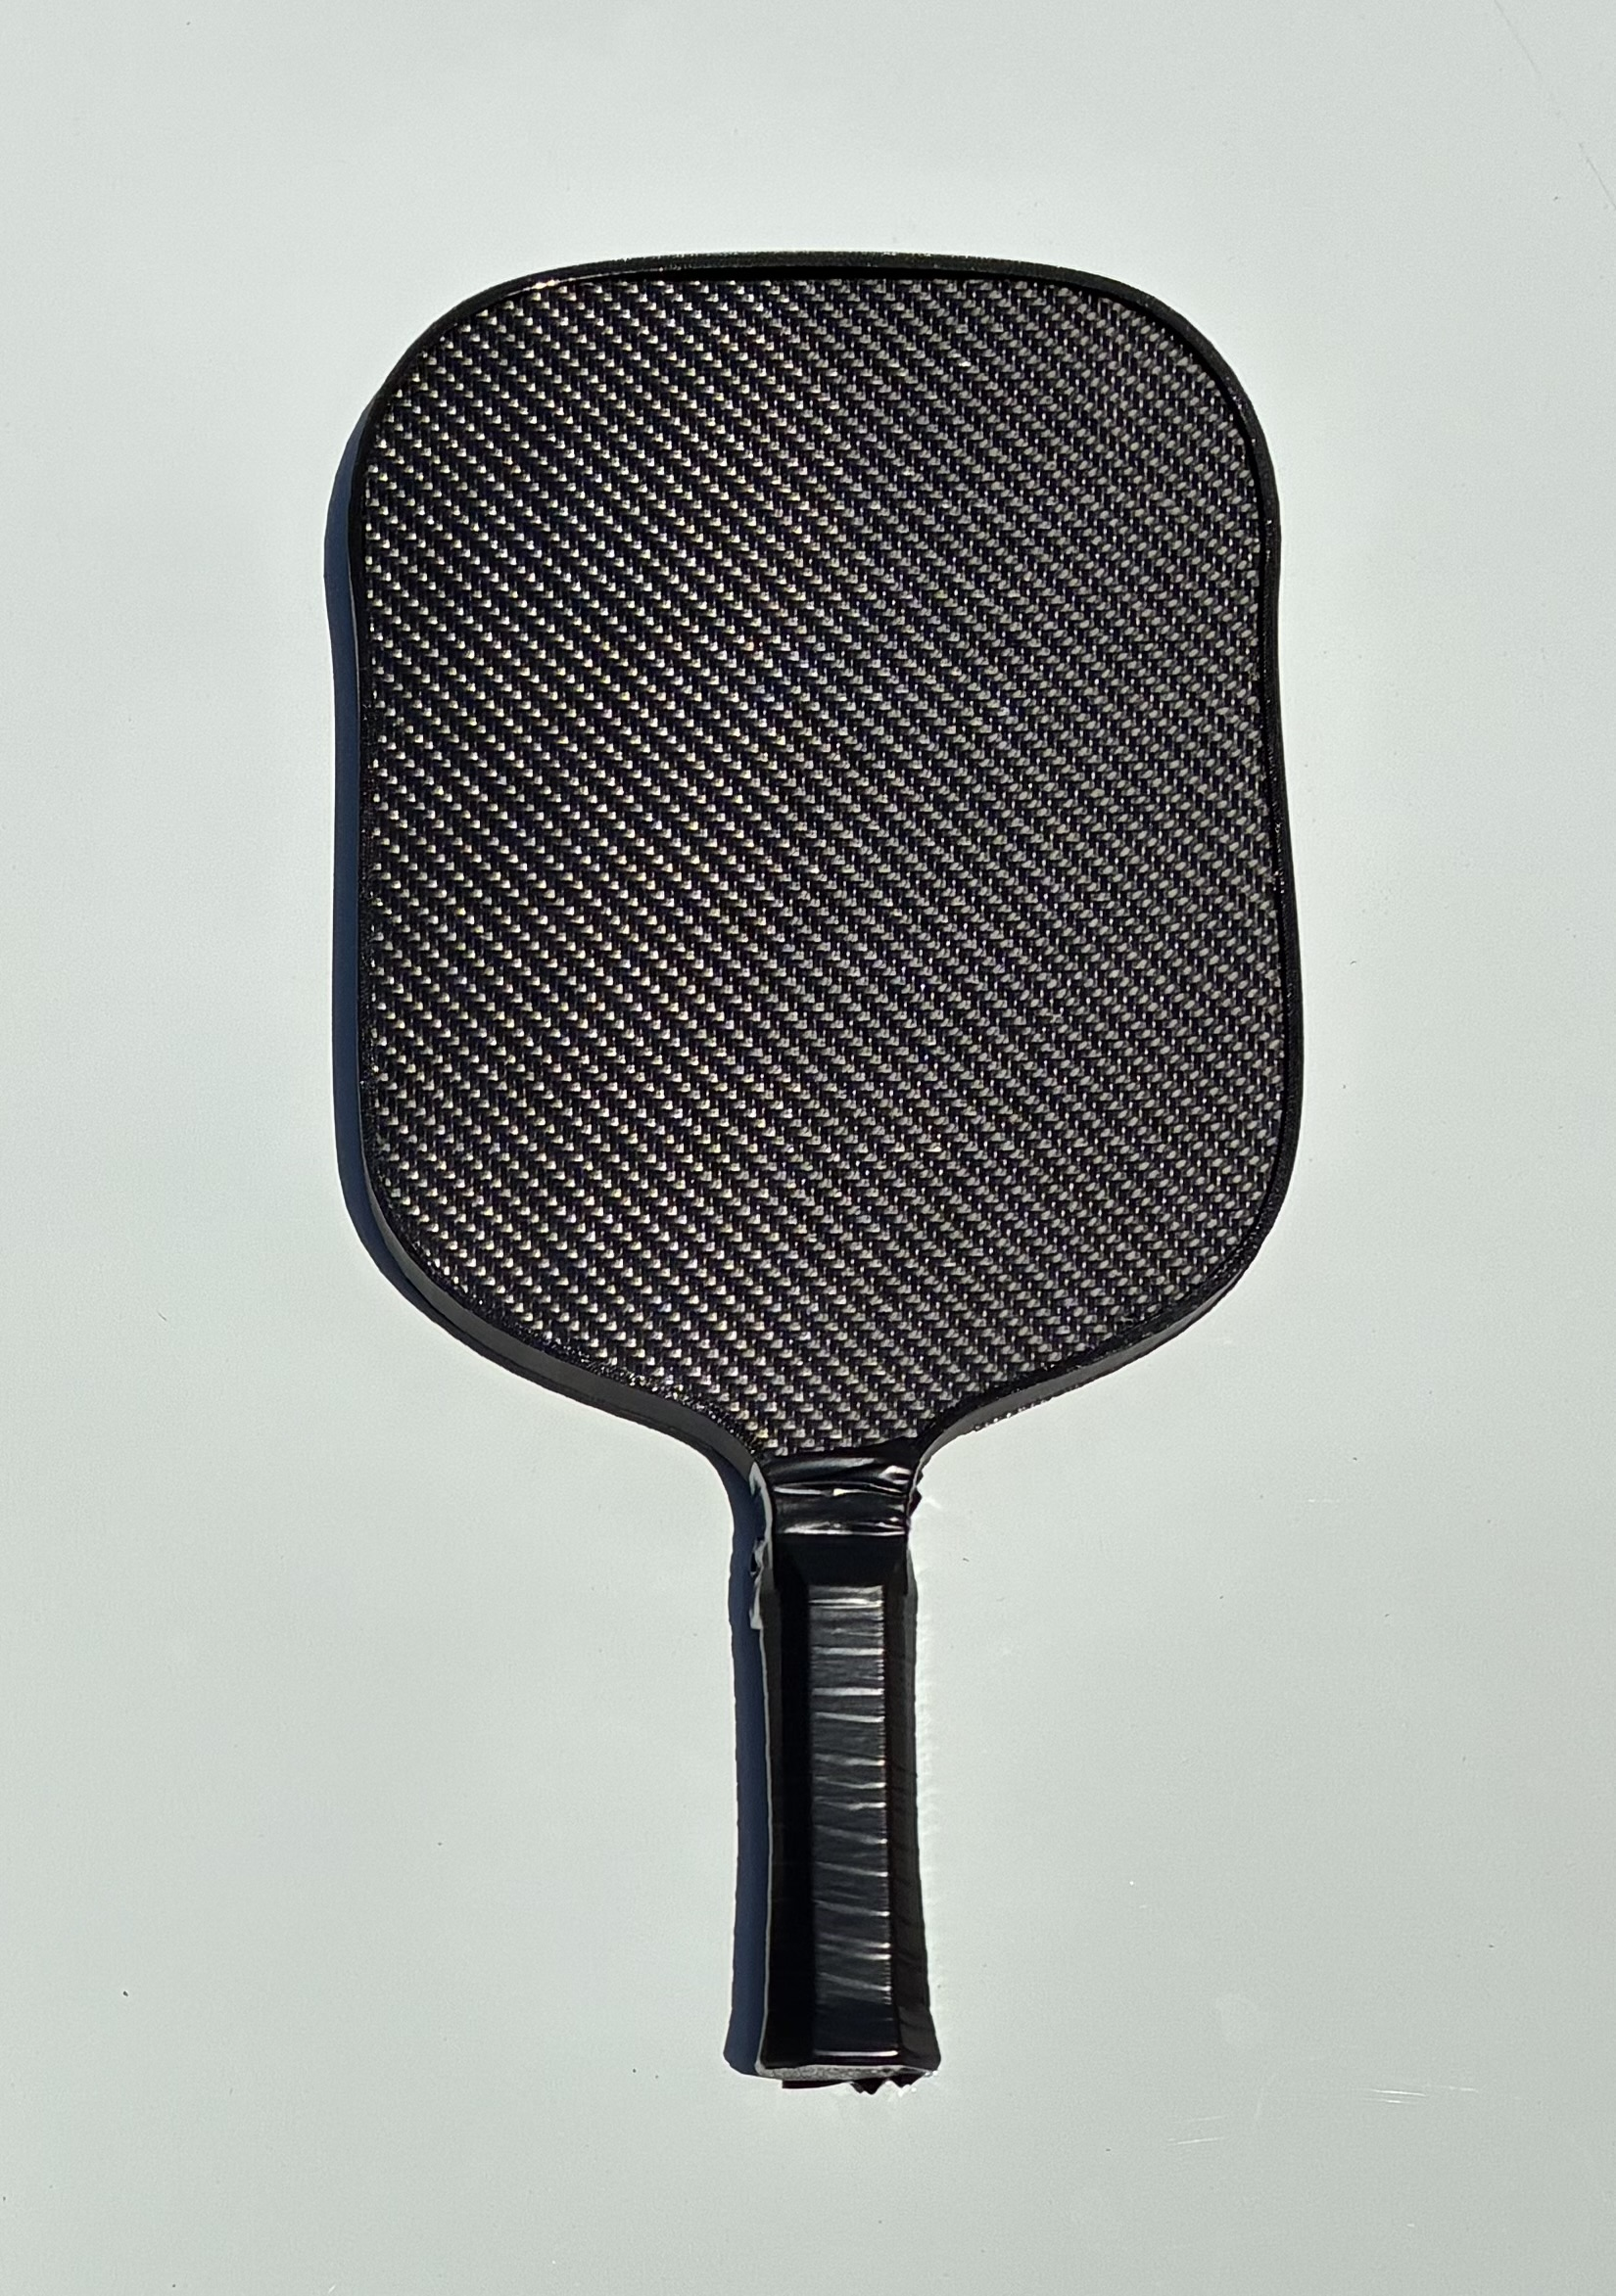
\includegraphics[
        width=3.72in,
        height=3.18in,
        keepaspectratio
    ]{full_assy}
};

\node[
    anchor=north,
    text=Muted,
    font=\sffamily\fontsize{6.9}{7.5}\selectfont
]
at ($(current page.north west)+(1.60in,-4.86in)$)
{Completed solo-built paddle assembly};

% ============================================================
% TOP CENTER — PROJECT OVERVIEW
% ============================================================

\fill[SoftGold,rounded corners=5pt]
    ($(current page.north west)+(2.95in,-1.62in)$)
    rectangle
    ($(current page.north west)+(5.53in,-4.86in)$);

\fill[PolyGold]
    ($(current page.north west)+(2.95in,-1.62in)$)
    rectangle
    ($(current page.north west)+(3.05in,-4.86in)$);

\node[
    anchor=north west,
    text=DeepGreen,
    font=\sffamily\bfseries\fontsize{8.0}{8.7}\selectfont
]
at ($(current page.north west)+(3.23in,-1.79in)$)
{PROJECT OVERVIEW};

\node[
    anchor=north west,
    align=left,
    text width=2.02in,
    text=Ink,
    font=\fontsize{7.05}{8.35}\selectfont
]
at ($(current page.north west)+(3.23in,-2.07in)$)
{
Independently designed and manufactured a lightweight prepreg
carbon-fiber pickleball paddle using a half-inch honeycomb
sandwich core, vacuum-bag consolidation, precision waterjet
trimming, and custom TPU and PLA components.

\vspace{5pt}

The project emphasized lightweight sandwich-composite design, repeatable manufacturing methods, dimensional accuracy, and the integration of custom 3D-printed TPU and PLA components into the final assembly.
};

\node[
    anchor=south west,
    align=left,
    text width=2.02in,
    text=PolyGold,
    font=\sffamily\bfseries\fontsize{6.65}{7.35}\selectfont
]
at ($(current page.north west)+(3.23in,-4.74in)$)
{
SOLE DESIGNER\\[2pt]
COMPOSITE FABRICATOR\\[2pt]
MANUFACTURING ENGINEER
};

% ============================================================
% TOP RIGHT — LAMINATE GRAPHIC
% ============================================================

\node[
    anchor=north west,
    inner sep=2.5pt,
    draw=DeepGreen,
    line width=0.65pt,
    rounded corners=5pt
]
at ($(current page.north west)+(5.71in,-1.62in)$)
{
    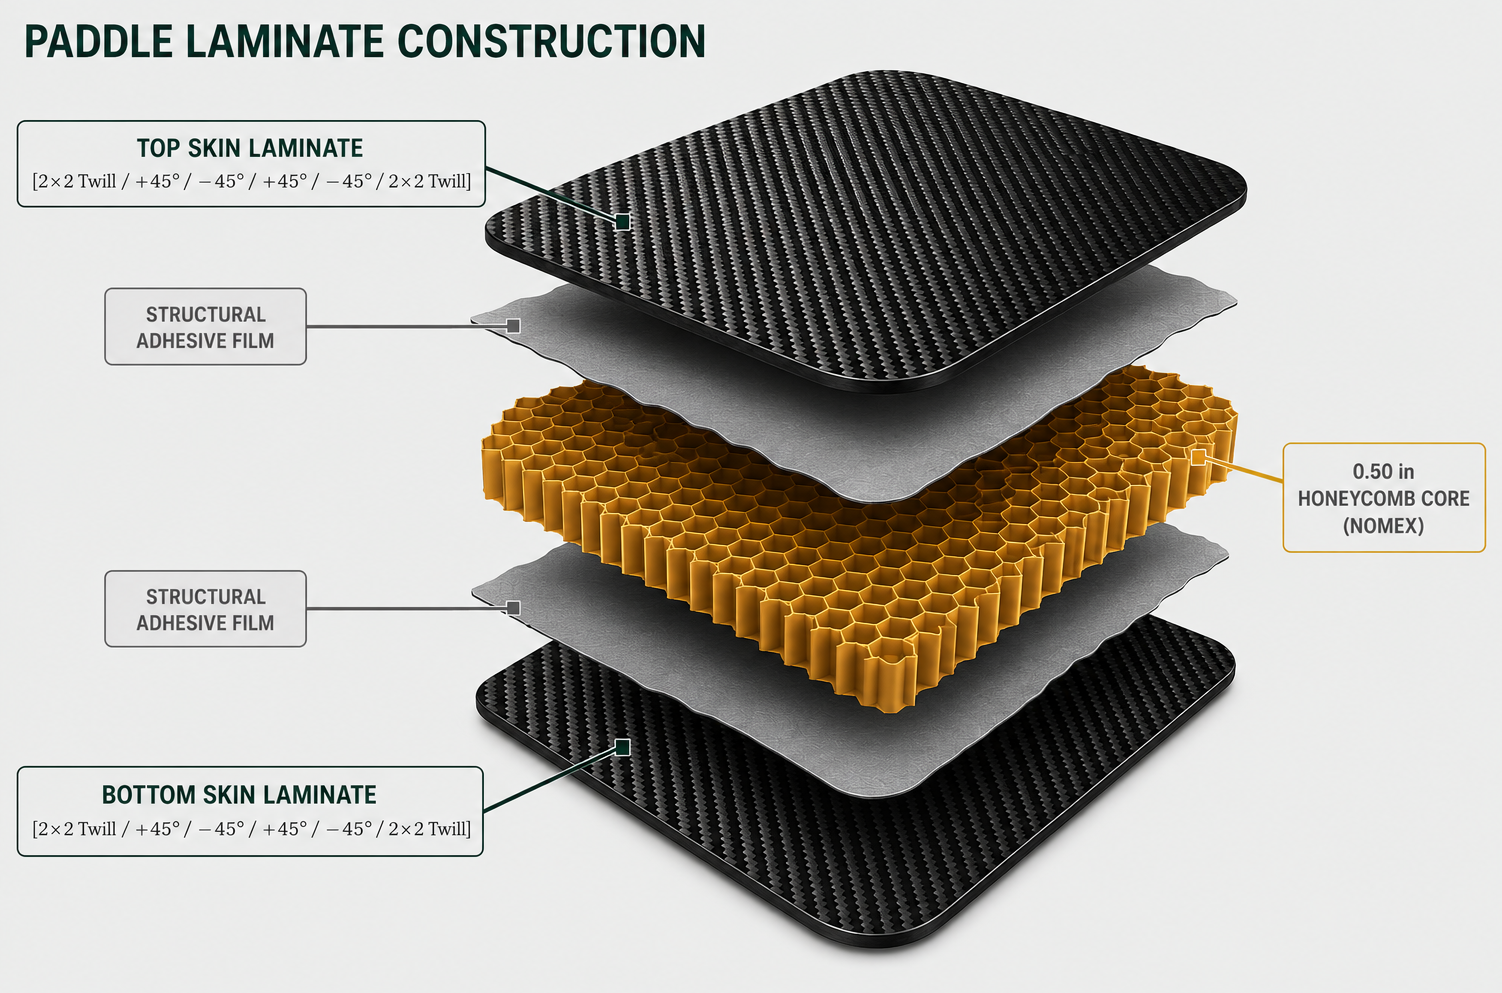
\includegraphics[
        width=4.80in,
        keepaspectratio
    ]{LAMINATE}
};

% ============================================================
% BOTTOM LEFT — SUPPORTING IMAGES
% ============================================================

\node[
    anchor=center,
    inner sep=3pt,
    draw=RuleGray,
    line width=0.55pt,
    rounded corners=4pt
]
at ($(current page.north west)+(1.12in,-5.98in)$)
{
    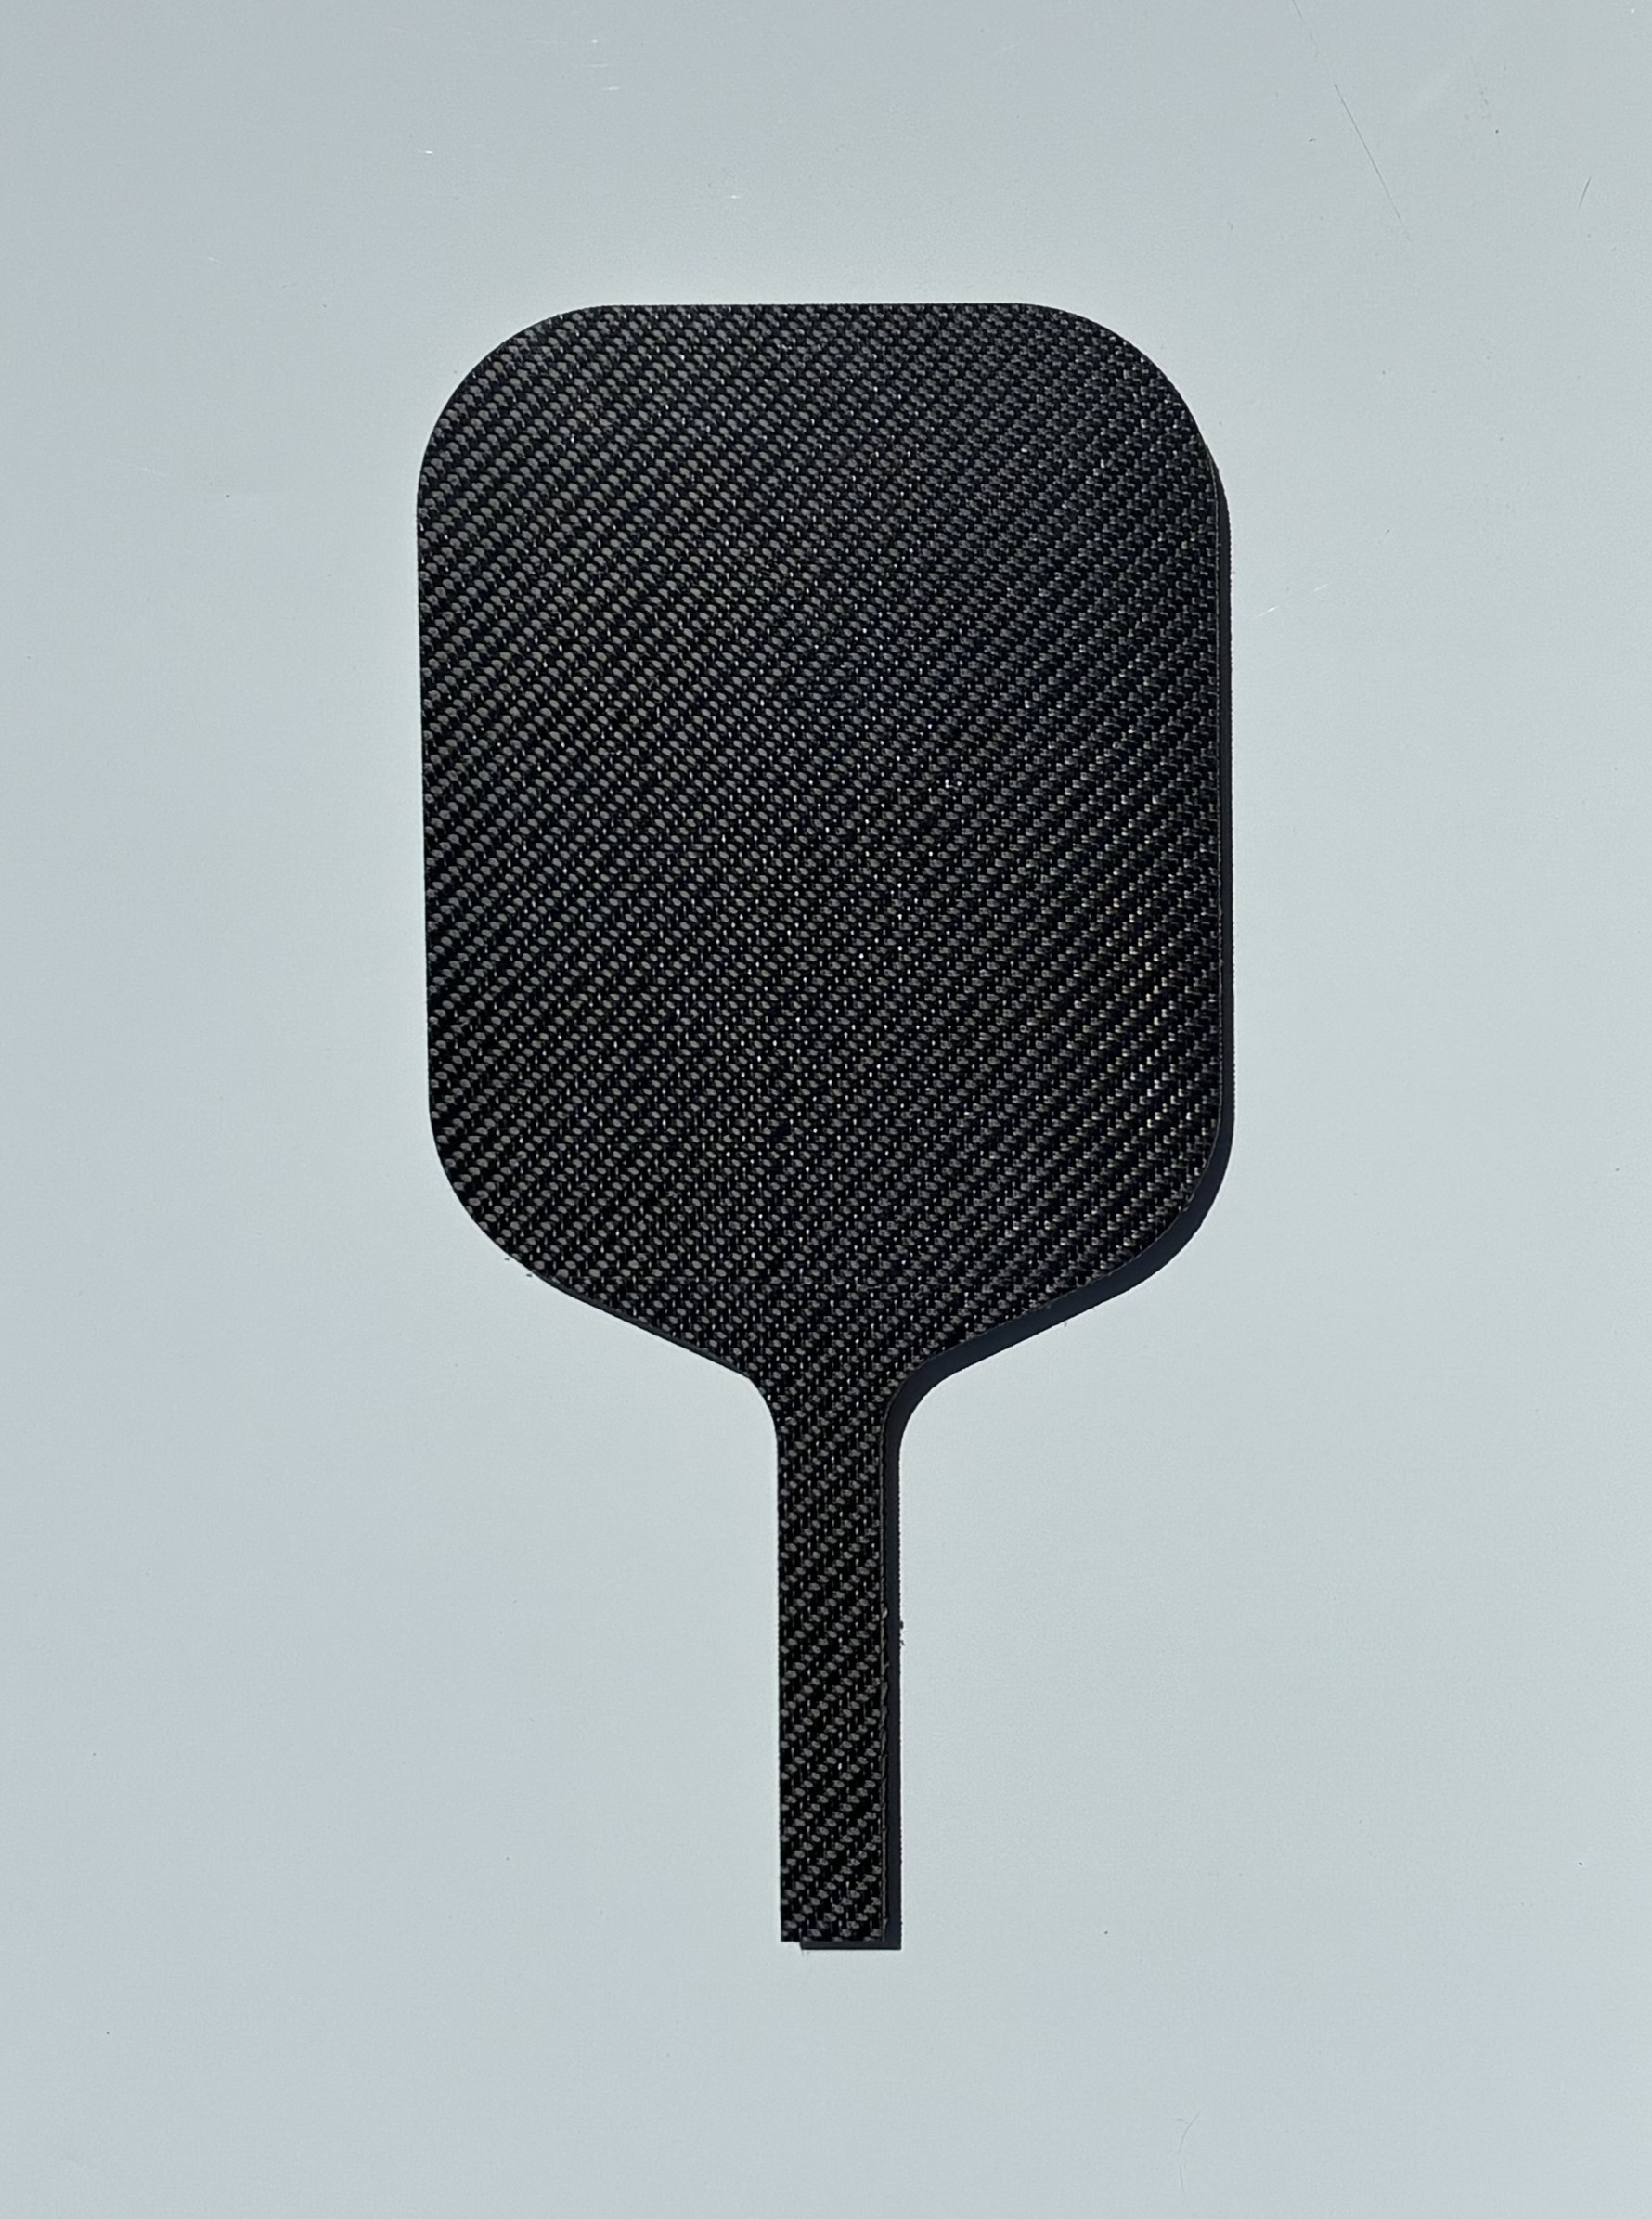
\includegraphics[
        width=1.30in,
        height=1.78in,
        keepaspectratio
    ]{front_view}
};

\node[
    anchor=center,
    inner sep=3pt,
    draw=RuleGray,
    line width=0.55pt,
    rounded corners=4pt
]
at ($(current page.north west)+(2.72in,-5.98in)$)
{
    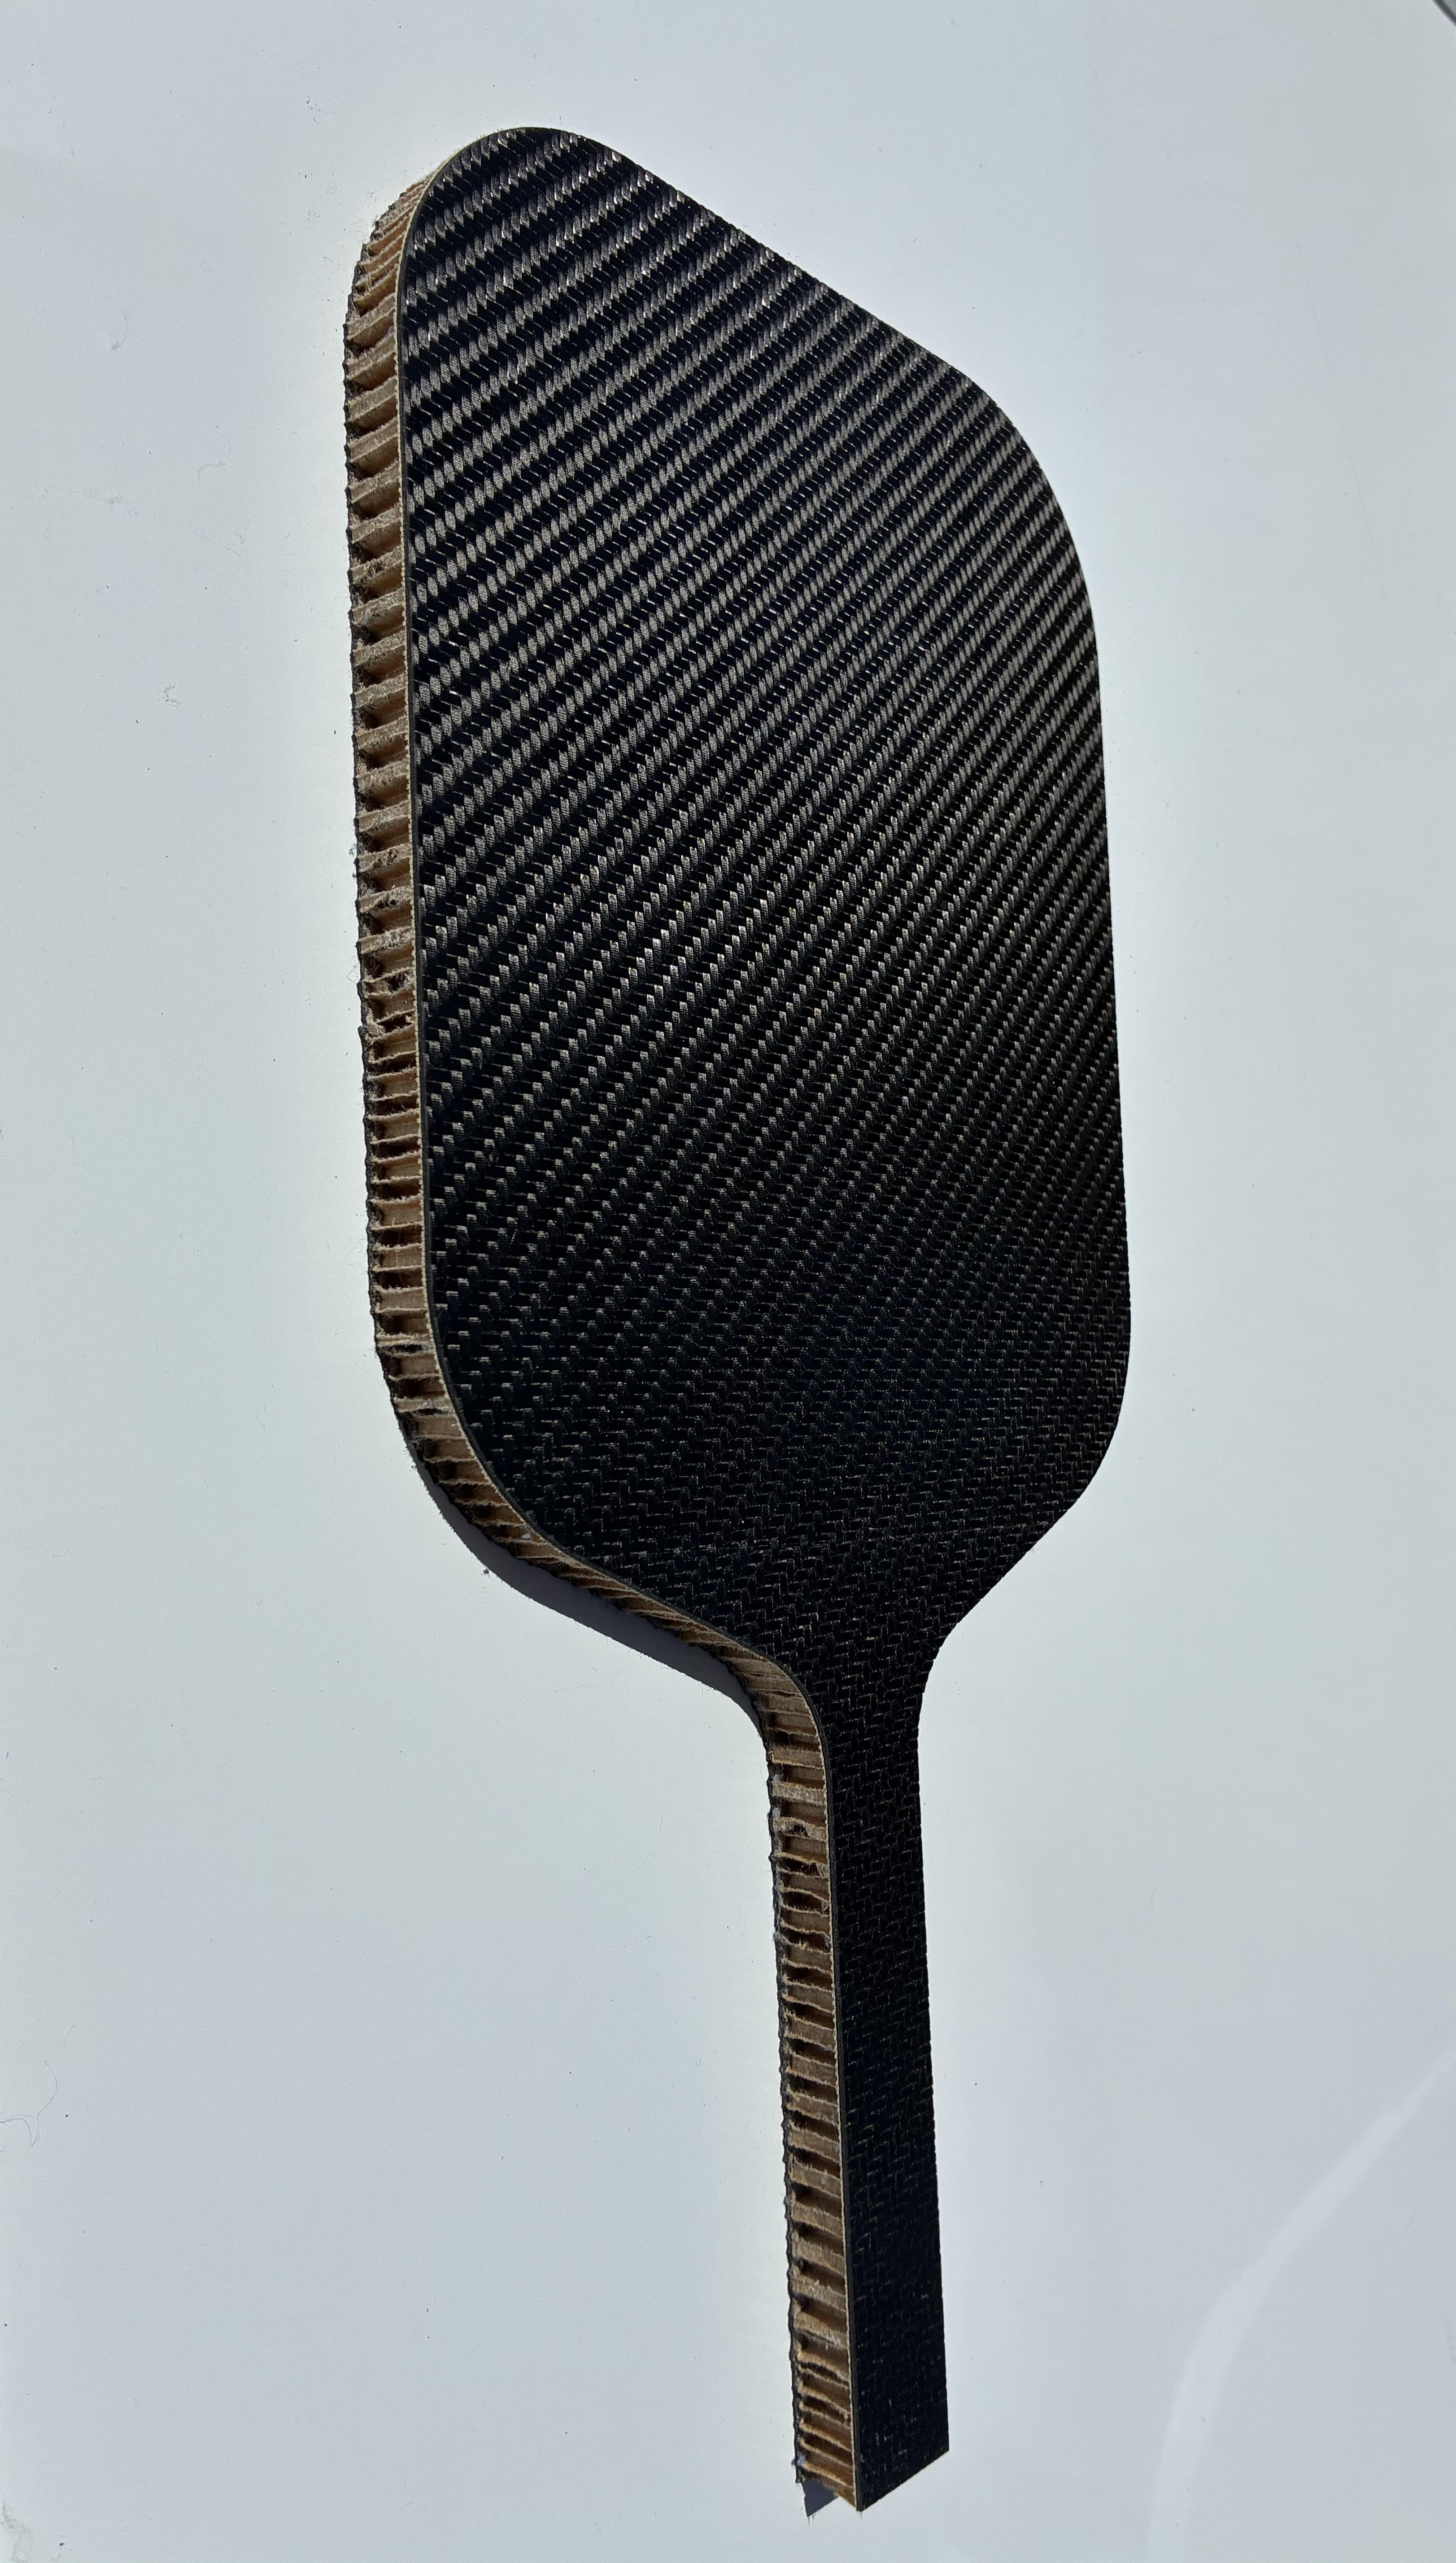
\includegraphics[
        width=1.30in,
        height=1.78in,
        keepaspectratio
    ]{side_core_view}
};

\node[
    anchor=center,
    inner sep=3pt,
    draw=RuleGray,
    line width=0.55pt,
    rounded corners=4pt
]
at ($(current page.north west)+(4.32in,-5.98in)$)
{
    \includegraphics[
        angle=-90,
        origin=c,
        width=1.30in,
        height=1.78in,
        keepaspectratio
    ]{waterjet}
};

\node[
    anchor=north,
    align=center,
    text width=1.38in,
    text=Muted,
    font=\sffamily\fontsize{6.5}{7.1}\selectfont
]
at ($(current page.north west)+(1.12in,-7.00in)$)
{Front view};

\node[
    anchor=north,
    align=center,
    text width=1.38in,
    text=Muted,
    font=\sffamily\fontsize{6.5}{7.1}\selectfont
]
at ($(current page.north west)+(2.72in,-7.00in)$)
{Core and edge profile};

\node[
    anchor=north,
    align=center,
    text width=1.38in,
    text=Muted,
    font=\sffamily\fontsize{6.5}{7.1}\selectfont
]
at ($(current page.north west)+(4.32in,-7.00in)$)
{Waterjet cutting setup};

% ============================================================
% BOTTOM RIGHT — MANUFACTURING HIGHLIGHTS
% ============================================================

\fill[SoftGreen,rounded corners=5pt]
    ($(current page.north west)+(5.18in,-5.05in)$)
    rectangle
    ($(current page.north east)+(-0.42in,-7.18in)$);

\draw[RuleGray,line width=0.55pt,rounded corners=5pt]
    ($(current page.north west)+(5.18in,-5.05in)$)
    rectangle
    ($(current page.north east)+(-0.42in,-7.18in)$);

\node[
    anchor=north west,
    text=DeepGreen,
    font=\sffamily\bfseries\fontsize{7.9}{8.6}\selectfont
]
at ($(current page.north west)+(5.44in,-5.20in)$)
{MANUFACTURING HIGHLIGHTS};

\node[
    anchor=north west,
    align=left,
    text width=5.05in,
    text=Ink,
    font=\fontsize{6.72}{7.82}\selectfont
]
at ($(current page.north west)+(5.44in,-5.49in)$)
{
\textbf{Consolidation.}
Vacuum bagging and distributed weight pressure maintained intimate contact
throughout the prepreg sandwich layup.\\[2.4pt]
\textbf{Surface quality.}
A scarce PTFE release film produced an unusually consistent matte finish
with a subtle sheen and minimal post-processing.\\[2.4pt]
\textbf{Waterjet stability.}
Perimeter weights restrained the cured stock against jet-induced lifting
and rotational moments during cutting.\\[2.4pt]
\textbf{Final assembly.}
A printed TPU edge band protected the carbon perimeter, while the PLA handle
used clearance cutouts to accommodate future stock-thickness and cutting variation.
};

% ============================================================
% RESOURCE LINK
% ============================================================

\node[
    anchor=north,
    align=center,
    text=DeepGreen,
    font=\sffamily\bfseries\fontsize{7.0}{7.6}\selectfont
]
at ($(current page.north)+(0,-7.42in)$)
{\href{\PaddleWaterjetVideo}
{\faPlayCircle\ WATERJET PICKLEBALL PADDLE DEMONSTRATION}};

% ============================================================
% FOOTER
% ============================================================

\node[
    anchor=south west,
    text=white,
    font=\sffamily\bfseries\fontsize{7.1}{7.7}\selectfont
]
at ($(current page.south west)+(0.42in,0.17in)$)
{\hyperlink{toro-results}{\faArrowLeft\ TORO COVER}};

\node[
    anchor=south,
    text=white,
    font=\sffamily\fontsize{7.0}{7.6}\selectfont
]
at ($(current page.south)+(0,0.17in)$)
{PICKLEBALL PADDLE \hspace{6pt} 1 / 1};

\node[
    anchor=south east,
    text=white,
    font=\sffamily\bfseries\fontsize{7.1}{7.7}\selectfont
]
at ($(current page.south east)+(-0.42in,0.17in)$)
{NEXT PROJECT \faArrowRight};

\end{tikzpicture}
%% ============================================================
% CARBON FIBER I-BEAM — SINGLE-PAGE PORTFOLIO CASE STUDY
% 01 Composites / Project 03
%
% IMPORTANT:
% 1. This file must NOT contain \documentclass, \begin{document},
%    or \end{document}.
% 2. In main.tex, place \input{ibeam_one_page} before \end{document}.
% 3. This script assumes the main portfolio preamble already defines:
%       DeepGreen, PolyGold, SoftGold, SoftGreen,
%       RuleGray, Muted, Ink
%    and loads tikz, graphicx, hyperref, and fontawesome5.
% 4. Upload these image files to Overleaf with the same names:
%       front view assembly graphic.png
%       Distributed weight with bolts.jpg
%       Stress Analysis on Generic CAD model.png
%       Beam Fiulure Delamination and cracking.jpeg
%       Three Point Bend Test.JPG
% ============================================================

\providecommand{\IBeamCompetitionGuidelines}
{https://drive.google.com/file/d/16S6MPVWWzPNKjXWVGKEySAi9i1f1BZYn/view?usp=sharing}

\providecommand{\IBeamBendTestVideo}
{https://drive.google.com/file/d/1LK_-pyK_y-a_4gDTiasz4uLUi95nAfrO/view?usp=drive_link}

\clearpage
\thispagestyle{empty}
\hypertarget{ibeam}{}
\null

\begin{tikzpicture}[remember picture,overlay]

% ============================================================
% BACKGROUND AND PAGE BARS
% ============================================================

\fill[white]
    (current page.south west)
    rectangle
    (current page.north east);

\fill[DeepGreen]
    (current page.north west)
    rectangle
    ($(current page.north east)+(0,-0.095in)$);

\fill[PolyGold]
    ($(current page.north west)+(0,-0.095in)$)
    rectangle
    ($(current page.north east)+(0,-0.14in)$);

\fill[DeepGreen]
    (current page.south west)
    rectangle
    ($(current page.south east)+(0,0.36in)$);

\fill[PolyGold]
    ($(current page.south west)+(0,0.36in)$)
    rectangle
    ($(current page.south east)+(0,0.405in)$);

% ============================================================
% HEADER
% ============================================================

\node[
    anchor=north west,
    text=PolyGold,
    font=\sffamily\bfseries\fontsize{8.1}{8.7}\selectfont
]
at ($(current page.north west)+(0.42in,-0.39in)$)
{01 COMPOSITES \hspace{5pt}/\hspace{5pt} PROJECT 03};

\node[
    anchor=north west,
    text=DeepGreen,
    font=\bfseries\fontsize{22.3}{23.3}\selectfont
]
at ($(current page.north west)+(0.40in,-0.67in)$)
{CARBON FIBER I-BEAM DESIGN \& TESTING};

\node[
    anchor=north west,
    text=Muted,
    font=\sffamily\fontsize{8.25}{9.0}\selectfont
]
at ($(current page.north west)+(0.42in,-1.12in)$)
{Cal Poly Composites Laboratory \hspace{7pt}\textbullet\hspace{7pt}
Individual Project \hspace{7pt}\textbullet\hspace{7pt}
Winter 2026 \hspace{7pt}\textbullet\hspace{7pt}
San Luis Obispo, California};

\fill[PolyGold]
    ($(current page.north west)+(0.42in,-1.36in)$)
    rectangle
    ($(current page.north west)+(6.10in,-1.315in)$);


% ============================================================
% TOP LEFT — ASSEMBLY ARCHITECTURE
% ============================================================

\node[
    anchor=north west,
    inner sep=2.6pt,
    draw=DeepGreen,
    line width=0.68pt,
    rounded corners=5pt
]
at ($(current page.north west)+(0.42in,-1.58in)$)
{
    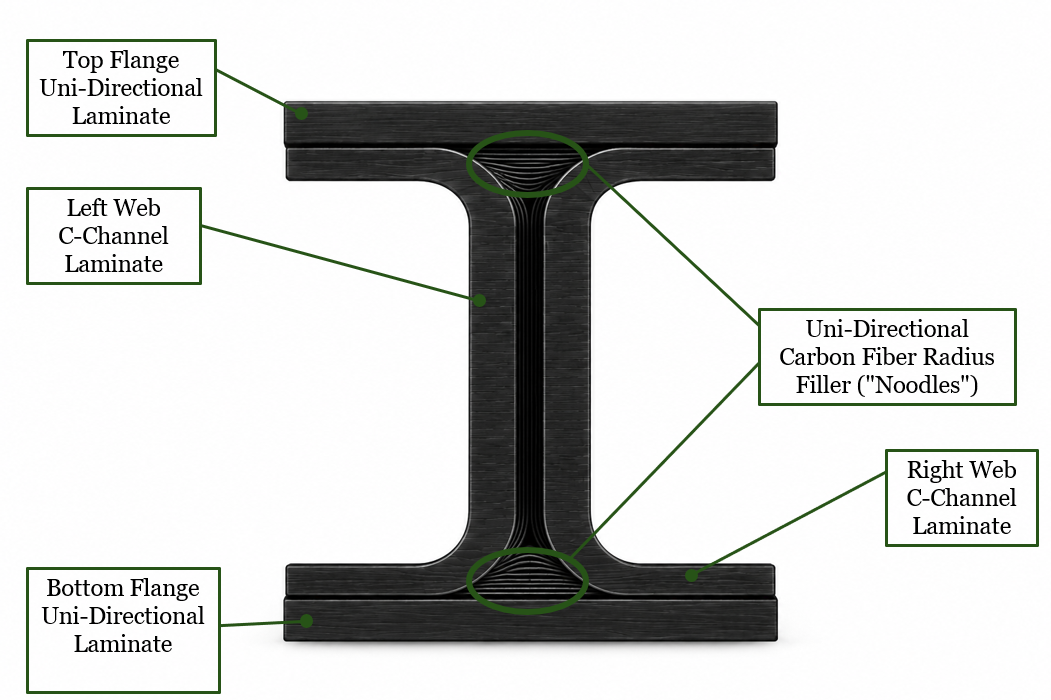
\includegraphics[
        width=3.55in,
        height=2.45in,
        keepaspectratio
    ]{front view assembly graphic.png}
};

\node[
    anchor=north,
    align=center,
    inner sep=0pt,
    text width=3.42in,
    text=Muted,
    font=\sffamily\fontsize{6.35}{7.05}\selectfont
]
at ($(current page.north west)+(2.195in,-4.12in)$)
{Four-piece laminate architecture with top and bottom flange laminates, paired C-channels, and longitudinal radius fillers};

% ============================================================
% TOP CENTER — PROJECT OVERVIEW + C-CHANNEL LAYUP
% ============================================================

\fill[SoftGold,rounded corners=5pt]
    ($(current page.north west)+(4.18in,-1.58in)$)
    rectangle
    ($(current page.north west)+(7.42in,-4.20in)$);

\fill[PolyGold]
    ($(current page.north west)+(4.18in,-1.58in)$)
    rectangle
    ($(current page.north west)+(4.28in,-4.20in)$);

\node[
    anchor=north west,
    text=DeepGreen,
    font=\sffamily\bfseries\fontsize{8.0}{8.7}\selectfont
]
at ($(current page.north west)+(4.48in,-1.76in)$)
{PROJECT OVERVIEW};

\node[
    anchor=north west,
    align=left,
    text width=2.64in,
    text=Ink,
    font=\fontsize{6.40}{7.45}\selectfont
]
at ($(current page.north west)+(4.48in,-2.04in)$)
{
A 24-inch carbon-fiber I-beam was manufactured from two molded
C-channel laminates, separate top and bottom flange laminates,
and longitudinal unidirectional radius fillers. The completed
684 g specimen sustained 28.2 kN (6,340 lbf) in three-point bending.\\[3pt]
\textbf{C-channel layup.}
Each channel used the same 12-ply sequence:
\mbox{$[+45/-45/0/+45/-45/0/0/-45/+45/0/-45/+45]$}.
The layup was completed twice, once for each channel.\\[3pt]
\textbf{Flange layups.}
Top flange: \mbox{$[90/0_6/90/0_6]$}. Bottom flange:
\mbox{$[90/0_6]$}, where $0_6$ denotes six consecutive 0-degree plies.
};

\node[
    anchor=south west,
    text=PolyGold,
    font=\sffamily\bfseries\fontsize{6.45}{7.1}\selectfont
]
at ($(current page.north west)+(4.48in,-4.03in)$)
{MASS: 684 g \hspace{8pt}\textbullet\hspace{8pt} PEAK LOAD: 28.2 kN \hspace{8pt}\textbullet\hspace{8pt} LENGTH: 24 in};

% ============================================================
% TOP RIGHT — C-CHANNEL MANUFACTURING
% ============================================================

\node[
    anchor=north west,
    inner sep=2.6pt,
    draw=DeepGreen,
    line width=0.68pt,
    rounded corners=5pt
]
at ($(current page.north west)+(7.62in,-1.58in)$)
{
    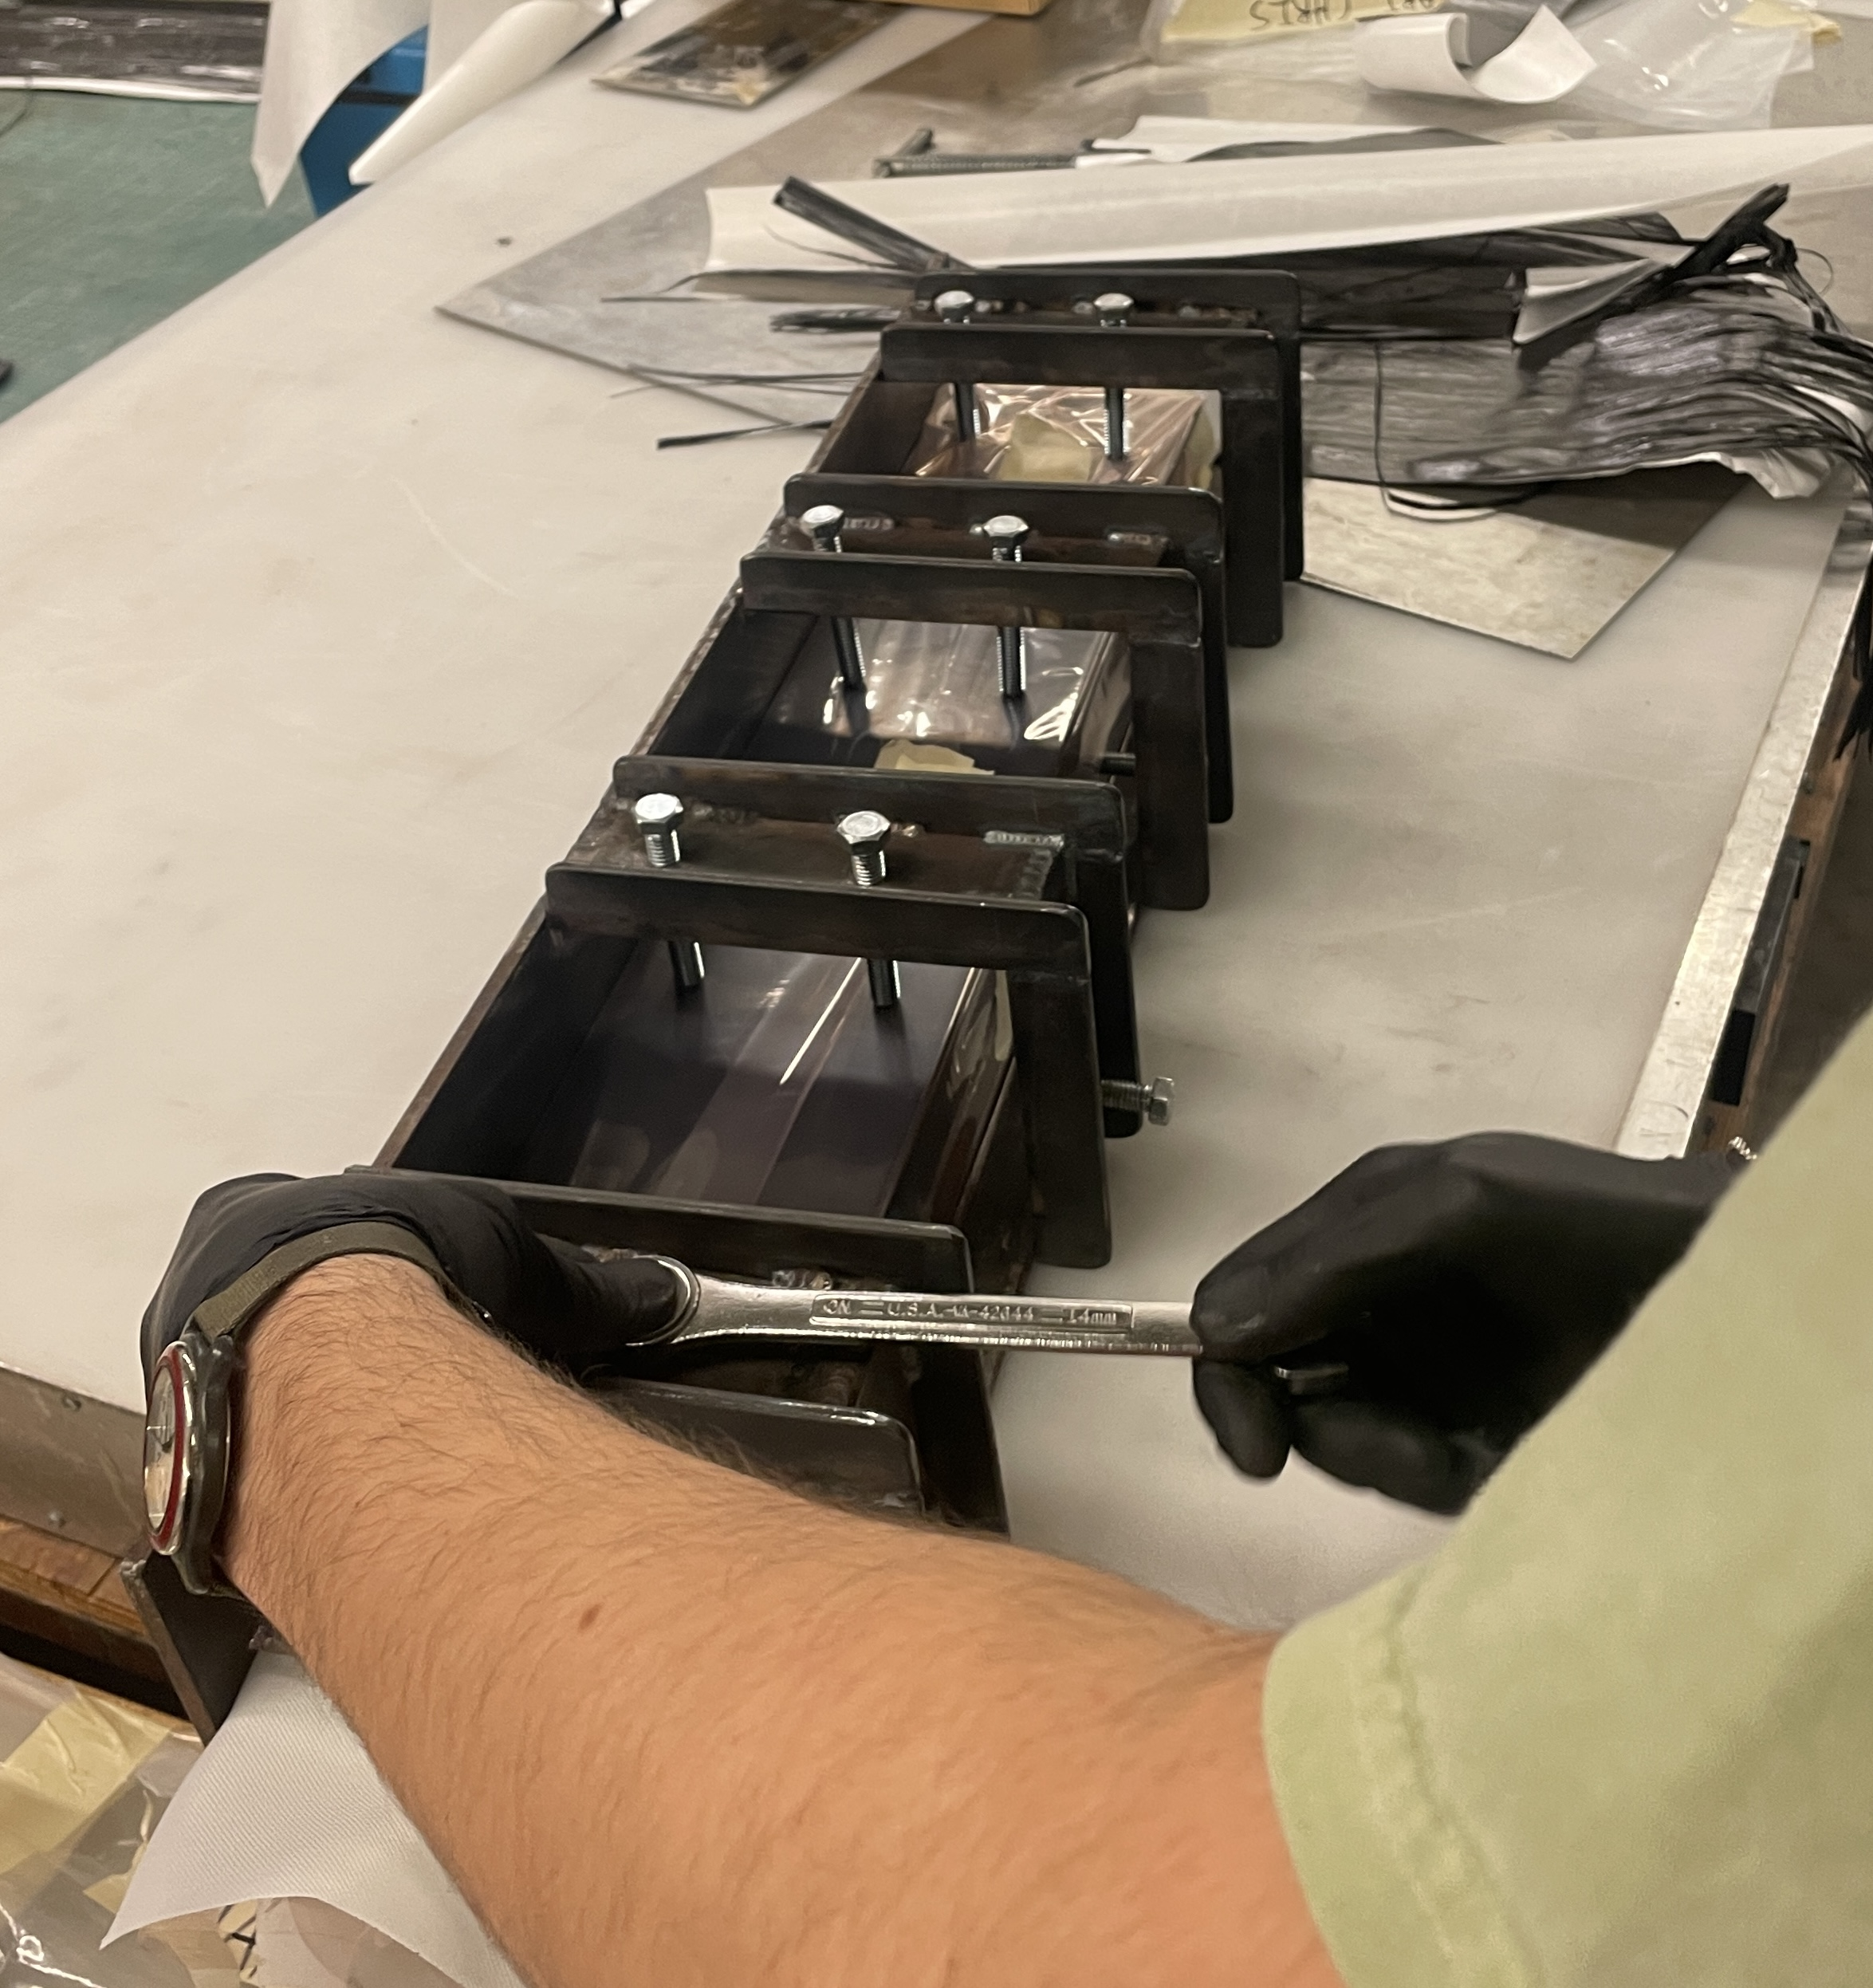
\includegraphics[
        width=3.55in,
        height=2.45in,
        keepaspectratio
    ]{Distributed weight with bolts.jpg}
};

\node[
    anchor=north,
    align=center,
    inner sep=0pt,
    text width=3.42in,
    text=Muted,
    font=\sffamily\fontsize{6.35}{7.05}\selectfont
]
at ($(current page.north west)+(9.395in,-4.12in)$)
{Distributed bolt pressure maintained alignment and consolidated the full beam assembly during cure};

% ============================================================
% CENTER ROW — MODEL, TEST, AND OBSERVED FAILURE
% ============================================================

\node[
    anchor=north west,
    inner sep=2.4pt,
    draw=RuleGray,
    line width=0.55pt,
    rounded corners=4pt
]
at ($(current page.north west)+(0.42in,-4.43in)$)
{
    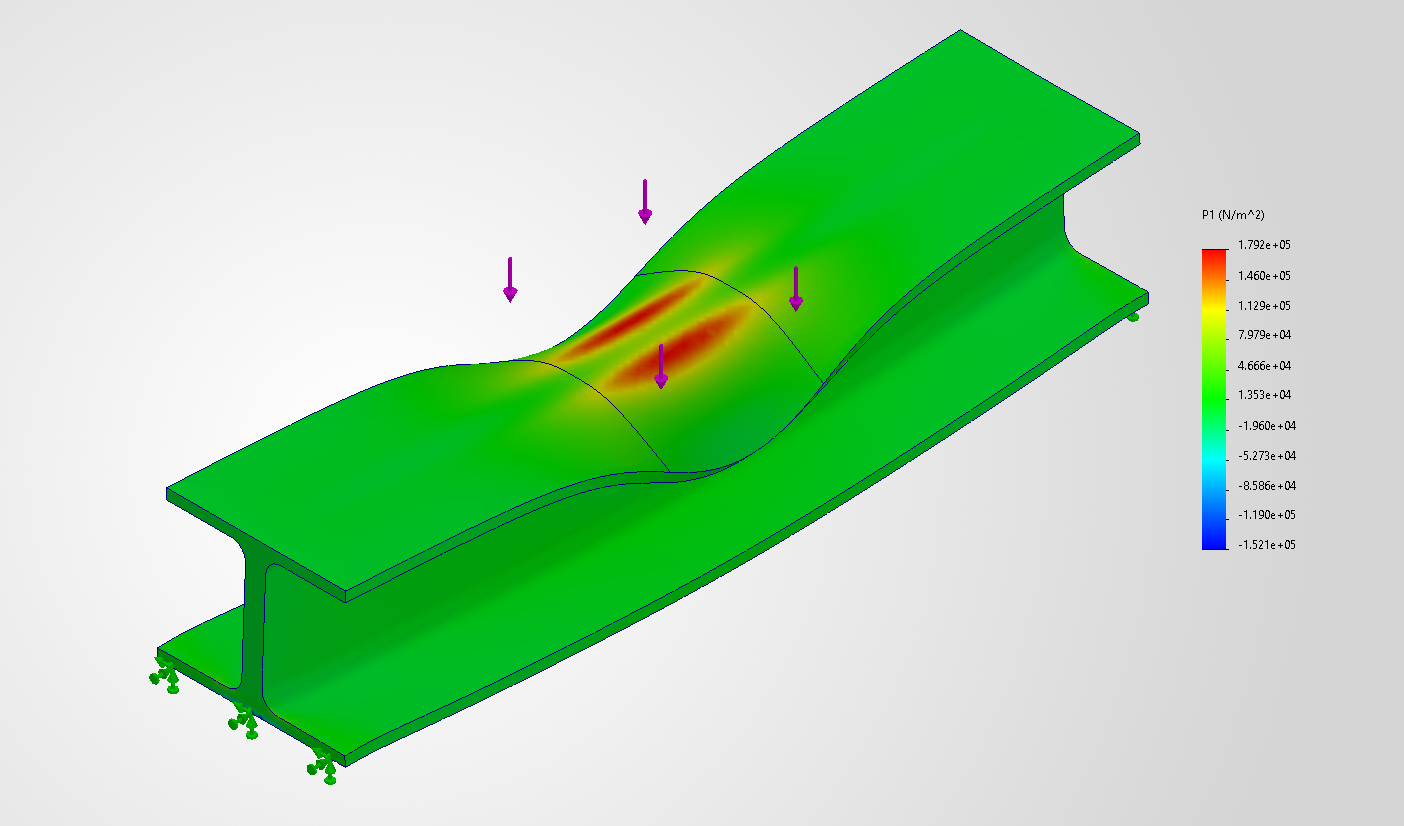
\includegraphics[
        width=3.33in,
        height=1.62in,
        keepaspectratio
    ]{Stress Analysis on Generic CAD model.png}
};

\node[
    anchor=north,
    align=center,
    inner sep=0pt,
    text width=3.20in,
    text=Muted,
    font=\sffamily\fontsize{6.20}{6.85}\selectfont
]
at ($(current page.north west)+(2.085in,-6.14in)$)
{Generic FEA predicted peak compressive stress beneath the center loading shoe};

\node[
    anchor=north west,
    inner sep=2.4pt,
    draw=RuleGray,
    line width=0.55pt,
    rounded corners=4pt
]
at ($(current page.north west)+(3.92in,-4.43in)$)
{
    \includegraphics[
        angle=180,
        origin=c,
        width=3.18in,
        height=1.62in,
        keepaspectratio
    ]{Three Point Bend Test.JPG}
};

\node[
    anchor=north,
    align=center,
    inner sep=0pt,
    text width=3.05in,
    text=Muted,
    font=\sffamily\fontsize{6.20}{6.85}\selectfont
]
at ($(current page.north west)+(5.510in,-6.14in)$)
{Experimental three-point bend test on the completed I-beam specimen};

\node[
    anchor=north west,
    inner sep=2.4pt,
    draw=RuleGray,
    line width=0.55pt,
    rounded corners=4pt
]
at ($(current page.north west)+(7.28in,-4.43in)$)
{
    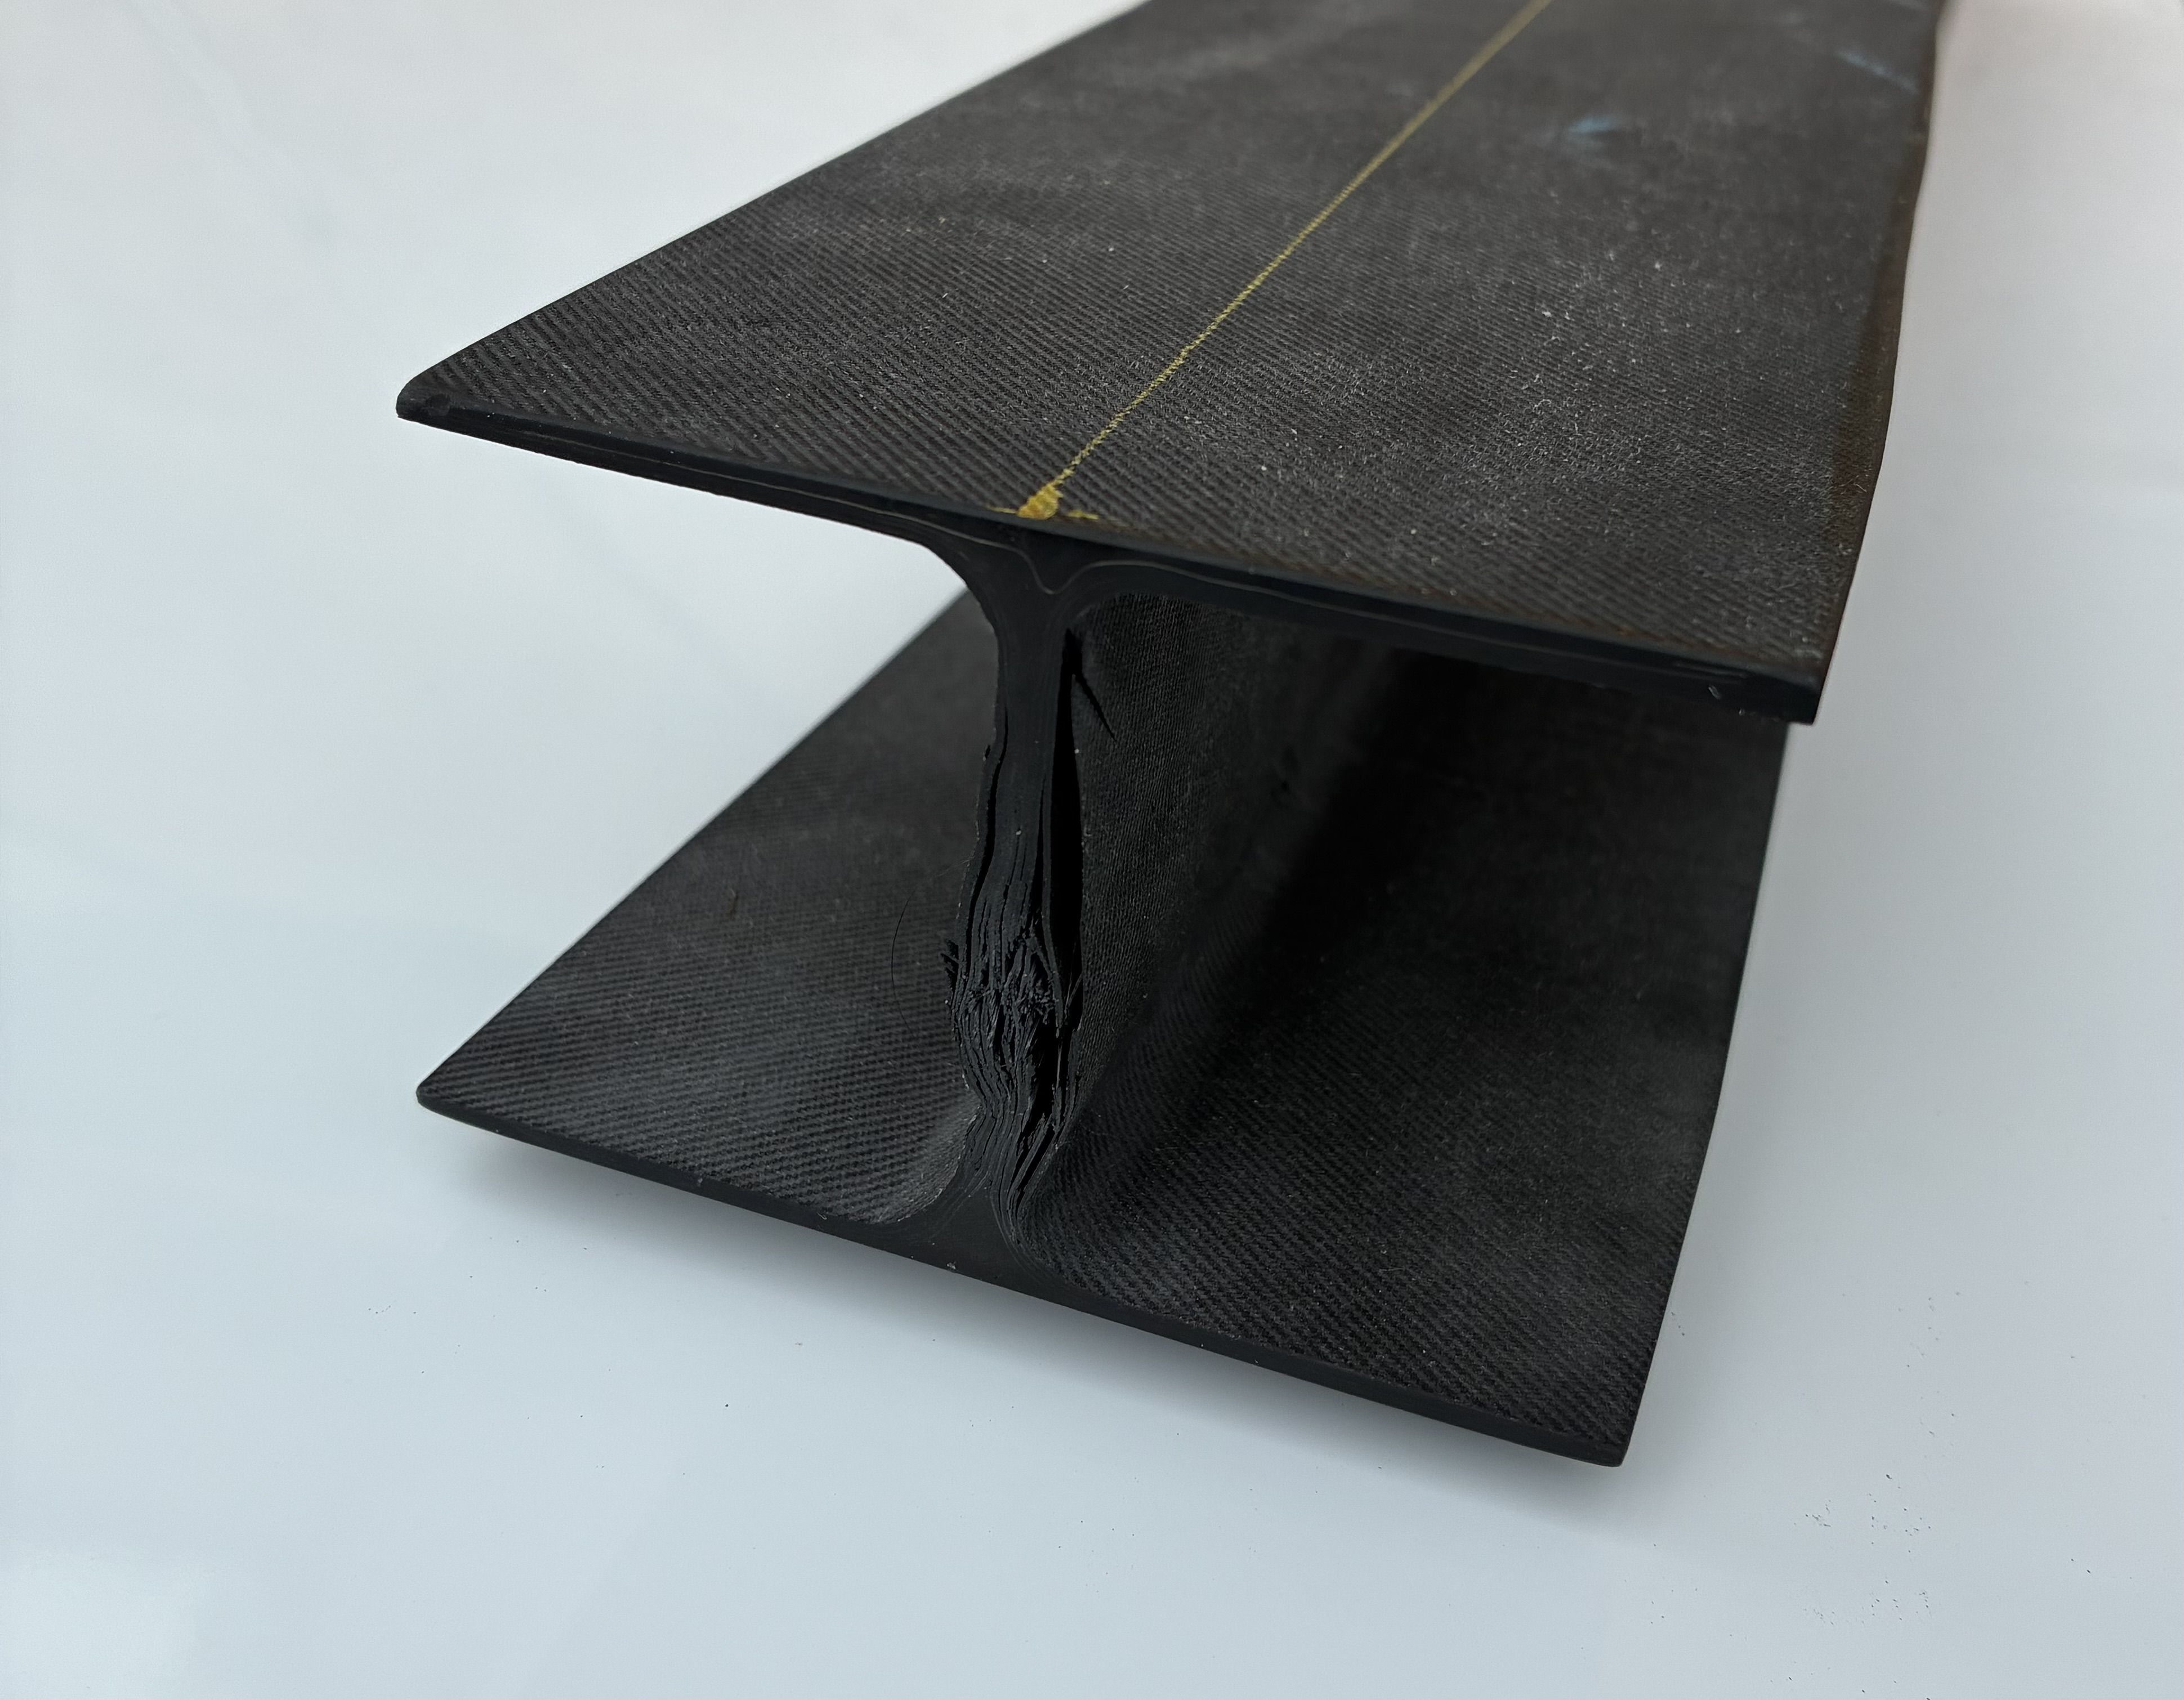
\includegraphics[
        width=3.65in,
        height=1.62in,
        keepaspectratio
    ]{Beam Fiulure Delamination and cracking.jpeg}
};

\node[
    anchor=north,
    align=center,
    inner sep=0pt,
    text width=3.50in,
    text=Muted,
    font=\sffamily\fontsize{6.20}{6.85}\selectfont
]
at ($(current page.north west)+(9.105in,-6.14in)$)
{Observed edge failure with delamination and longitudinal crack propagation};

% ============================================================
% BOTTOM LEFT — MANUFACTURING PROCESS
% ============================================================

\fill[SoftGreen,rounded corners=5pt]
    ($(current page.north west)+(0.42in,-6.43in)$)
    rectangle
    ($(current page.north west)+(5.30in,-7.18in)$);

\draw[RuleGray,line width=0.55pt,rounded corners=5pt]
    ($(current page.north west)+(0.42in,-6.43in)$)
    rectangle
    ($(current page.north west)+(5.30in,-7.18in)$);

\node[
    anchor=north west,
    text=DeepGreen,
    font=\sffamily\bfseries\fontsize{7.65}{8.35}\selectfont
]
at ($(current page.north west)+(0.66in,-6.57in)$)
{MANUFACTURING APPROACH};

\node[
    anchor=north west,
    align=left,
    text width=4.38in,
    text=Ink,
    font=\fontsize{6.20}{7.15}\selectfont
]
at ($(current page.north west)+(0.66in,-6.82in)$)
{
The separately molded channels were aligned with longitudinal carbon-fiber
``noodles'' filling the radius-induced flange voids. Top and bottom flanges
were then installed, and the full assembly was consolidated in a custom
steel fixture using distributed bolt pressure along the beam length.
};

% ============================================================
% BOTTOM RIGHT — FAILURE ANALYSIS AND NEXT ITERATION
% ============================================================

\fill[SoftGold,rounded corners=5pt]
    ($(current page.north west)+(5.52in,-6.43in)$)
    rectangle
    ($(current page.north east)+(-0.42in,-7.18in)$);

\fill[PolyGold]
    ($(current page.north west)+(5.52in,-6.43in)$)
    rectangle
    ($(current page.north west)+(5.62in,-7.18in)$);

\node[
    anchor=north west,
    text=DeepGreen,
    font=\sffamily\bfseries\fontsize{7.65}{8.35}\selectfont
]
at ($(current page.north west)+(5.82in,-6.57in)$)
{FAILURE ANALYSIS AND NEXT ITERATION};

\node[
    anchor=north west,
    align=left,
    text width=4.72in,
    text=Ink,
    font=\fontsize{6.14}{7.08}\selectfont
]
at ($(current page.north west)+(5.82in,-6.82in)$)
{
The model suggested a center-span compression failure, but the physical beam
failed near its edge. This mismatch indicates that local consolidation defects
likely enabled premature delamination. A future build should use staged vacuum
debulking after each ply group rather than relying only on manual rolling before
final fixture consolidation.
};

% ============================================================
% RESOURCE LINKS
% ============================================================

\node[
    anchor=north,
    align=center,
    text=DeepGreen,
    font=\sffamily\bfseries\fontsize{6.75}{7.35}\selectfont
]
at ($(current page.north)+(0,-7.43in)$)
{
\href{\IBeamCompetitionGuidelines}{\faFilePdf\ COMPETITION GUIDELINES}
\hspace{16pt}
\href{\IBeamBendTestVideo}{\faPlayCircle\ THREE-POINT BEND TEST VIDEO}
};

% ============================================================
% FOOTER
% ============================================================

\node[
    anchor=south west,
    text=white,
    font=\sffamily\bfseries\fontsize{7.1}{7.7}\selectfont
]
at ($(current page.south west)+(0.42in,0.17in)$)
{\hyperlink{pickleball}{\faArrowLeft\ PICKLEBALL PADDLE}};

\node[
    anchor=south,
    text=white,
    font=\sffamily\fontsize{7.0}{7.6}\selectfont
]
at ($(current page.south)+(0,0.17in)$)
{CARBON FIBER I-BEAM \hspace{6pt} 1 / 1};

\node[
    anchor=south east,
    text=white,
    font=\sffamily\bfseries\fontsize{7.1}{7.7}\selectfont
]
at ($(current page.south east)+(-0.42in,0.17in)$)
{NEXT PROJECT \faArrowRight};

\end{tikzpicture}
\input{fuselage}
\clearpage


%\clearpage

\clearpage
.
% 2. In main.tex, place 
% ============================================================
% TORO COVER — THREE-PAGE PORTFOLIO CASE STUDY
% Pages 3–5 of the complete portfolio
%
% IMPORTANT:
% 1. This file must NOT contain \documentclass, \begin{document},
%    \end{document}, or 
% ============================================================
% TORO COVER — THREE-PAGE PORTFOLIO CASE STUDY
% Pages 3–5 of the complete portfolio
%
% IMPORTANT:
% 1. This file must NOT contain \documentclass, \begin{document},
%    \end{document}, or 
% ============================================================
% TORO COVER — THREE-PAGE PORTFOLIO CASE STUDY
% Pages 3–5 of the complete portfolio
%
% IMPORTANT:
% 1. This file must NOT contain \documentclass, \begin{document},
%    \end{document}, or \input{toro}.
% 2. In main.tex, place \input{toro} before \end{document}.
% 3. Image references use the original Overleaf base filenames
%    without extensions.
% ============================================================



% ============================================================
% CLICKABLE PROJECT RESOURCES
% All links use the exact Google Drive resources supplied.
% ============================================================
\providecommand{\ToroDrawingLink}{https://drive.google.com/file/d/1A7-7wMnRNLuQDaTgxeuUCBsGNqyXzOGV/view?usp=sharing}
\providecommand{\ToroDimensionsLink}{https://drive.google.com/file/d/13sw3BNJvE8GdzlRffxoF2n5r9Gzxide7/view?usp=sharing}
\providecommand{\ToroProblemLink}{https://drive.google.com/file/d/1zHtl8zrb13F1yeN74ptawpfS5UM_xsuw/view?usp=drive_link}
\providecommand{\ToroReportLink}{https://drive.google.com/file/d/1ULZ-P46lFsC2x29ZfmRVIKgYnr9o8hMt/view?usp=drive_link}
\providecommand{\ToroPosterLink}{https://drive.google.com/file/d/1vKiKaJUcHQb_db-FkZnRF6EvtuM4hKyS/view?usp=drive_link}
\providecommand{\ToroDeploymentLink}{https://drive.google.com/file/d/1XJx34o80_mZPTl7xy93HtWAgtS3ThhvY/view?usp=drive_link}
\providecommand{\ToroRemovalLink}{https://drive.google.com/file/d/1O7xYeyB67NUwT-j1B1HeiCcHnZDYjk6_/view?usp=drive_link}

% ============================================================
% PAGE 1 — PROJECT OVERVIEW, OWNERSHIP, AND ARCHITECTURE
% ============================================================

\clearpage
\thispagestyle{empty}
\hypertarget{toro}{}
\null

\begin{tikzpicture}[remember picture,overlay]

% Background
\fill[white]
    (current page.south west)
    rectangle
    (current page.north east);

% Page bars
\fill[DeepGreen]
    (current page.north west)
    rectangle
    ($(current page.north east)+(0,-0.095in)$);

\fill[PolyGold]
    ($(current page.north west)+(0,-0.095in)$)
    rectangle
    ($(current page.north east)+(0,-0.14in)$);

\fill[DeepGreen]
    (current page.south west)
    rectangle
    ($(current page.south east)+(0,0.36in)$);

\fill[PolyGold]
    ($(current page.south west)+(0,0.36in)$)
    rectangle
    ($(current page.south east)+(0,0.405in)$);

% Header
\node[
    anchor=north west,
    text=PolyGold,
    font=\sffamily\bfseries\fontsize{8.1}{8.7}\selectfont
]
at ($(current page.north west)+(0.42in,-0.39in)$)
{01 COMPOSITES \hspace{5pt}/\hspace{5pt} PROJECT 01};

\node[
    anchor=north west,
    text=DeepGreen,
    font=\bfseries\fontsize{23.5}{24.5}\selectfont
]
at ($(current page.north west)+(0.40in,-0.67in)$)
{TORO CARBON FIBER SAFETY COVER};

\node[
    anchor=north west,
    text=Muted,
    font=\sffamily\fontsize{8.4}{9.2}\selectfont
]
at ($(current page.north west)+(0.42in,-1.12in)$)
{Cal Poly Composites Laboratory \hspace{7pt}\textbullet\hspace{7pt}
Team Project \hspace{7pt}\textbullet\hspace{7pt}
Fall--Spring 2026 \hspace{7pt}\textbullet\hspace{7pt}
San Luis Obispo, California};

\fill[PolyGold]
    ($(current page.north west)+(0.42in,-1.37in)$)
    rectangle
    ($(current page.north west)+(6.1in,-1.325in)$);

% Challenge text
\node[
    anchor=north west,
    text=DeepGreen,
    font=\sffamily\bfseries\fontsize{8.1}{8.8}\selectfont
]
at ($(current page.north west)+(0.43in,-1.61in)$)
{THE CHALLENGE};

\node[
    anchor=north west,
    align=left,
    text width=4.47in,
    text=Ink,
    font=\fontsize{8.05}{9.65}\selectfont
]
at ($(current page.north west)+(0.43in,-1.84in)$)
{
Develop a lightweight cover for a 6 ft by 6 ft in-ground spa
that could be deployed by one person, stored compactly,
provide insulation, resist a poolside environment, and maintain
a refined appearance. The sponsor supplied an ambitious but
intentionally broad project statement, requiring the team to
define the product architecture, priorities, manufacturing
strategy, and realistic path toward future commercialization.
};

% Role box
\fill[SoftGold,rounded corners=5pt]
    ($(current page.north west)+(0.42in,-2.88in)$)
    rectangle
    ($(current page.north west)+(4.98in,-4.58in)$);

\fill[PolyGold]
    ($(current page.north west)+(0.42in,-2.88in)$)
    rectangle
    ($(current page.north west)+(0.52in,-4.58in)$);

\node[
    anchor=north west,
    text=DeepGreen,
    font=\sffamily\bfseries\fontsize{8.1}{8.8}\selectfont
]
at ($(current page.north west)+(0.66in,-3.02in)$)
{MY ROLE — DESIGN \& MANUFACTURING LEAD};

\node[
    anchor=north west,
    align=left,
    text width=4.02in,
    text=Ink,
    font=\fontsize{7.05}{8.15}\selectfont
]
at ($(current page.north west)+(0.66in,-3.27in)$)
{
\textbullet\ Modeled every custom part and the complete assembly\\[1.5pt]
\textbullet\ Produced the engineering drawing package independently\\[1.5pt]
\textbullet\ Developed the composite-panel manufacturing process\\[1.5pt]
\textbullet\ Created all waterjet DXFs and manufacturing geometry\\[1.5pt]
\textbullet\ Trained teammates in wet layup and vacuum bagging\\[1.5pt]
\textbullet\ Presented feasibility, scope, and tradeoffs to the sponsor
};

% Large deployed foam-model image
\node[anchor=center,inner sep=0pt]
at ($(current page.north west)+(8.00in,-3.04in)$)
{
    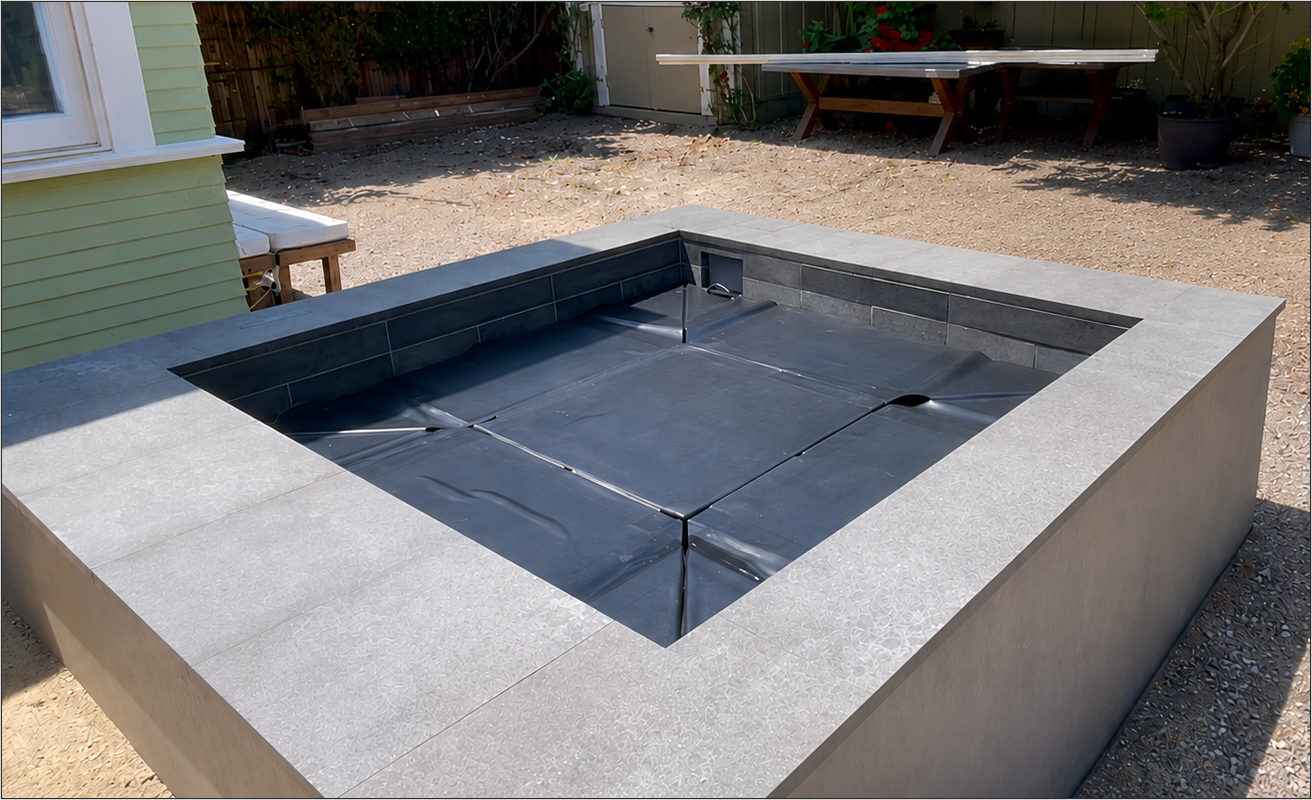
\includegraphics[
        width=5.55in,
        height=2.78in,
        keepaspectratio
    ]{deployed_functional_prototype}
};

\draw[DeepGreen,line width=0.8pt,rounded corners=7pt]
    ($(current page.north west)+(5.16in,-1.61in)$)
    rectangle
    ($(current page.north east)+(-0.42in,-4.47in)$);

\node[
    anchor=north west,
    text=Muted,
    font=\sffamily\fontsize{6.2}{6.9}\selectfont
]
at ($(current page.north west)+(5.18in,-4.54in)$)
{Functional foam model deployed over the sponsor's in-ground spa.};

% Image-strip title
\node[
    anchor=north west,
    text=DeepGreen,
    font=\sffamily\bfseries\fontsize{8.1}{8.8}\selectfont
]
at ($(current page.north west)+(0.43in,-4.78in)$)
{PRODUCT DEVELOPMENT AND FINAL ARCHITECTURE};

% Five-image development strip — CAD-first sequence
% Image 1: topside CAD
\node[anchor=center,inner sep=0pt]
at ($(current page.north west)+(1.47in,-5.73in)$)
{
    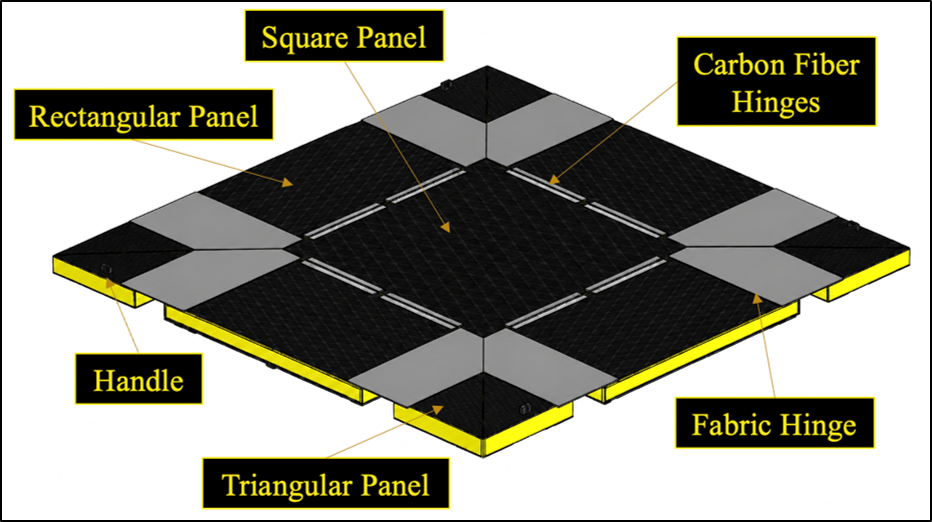
\includegraphics[
        width=1.92in,
        height=1.30in,
        keepaspectratio
    ]{Toro_Cover_topside_Cad}
};
\draw[RuleGray,line width=0.55pt,rounded corners=4pt]
    ($(current page.north west)+(0.43in,-5.04in)$)
    rectangle
    ($(current page.north west)+(2.51in,-6.43in)$);

% Image 2: underside CAD
\node[anchor=center,inner sep=0pt]
at ($(current page.north west)+(3.66in,-5.73in)$)
{
    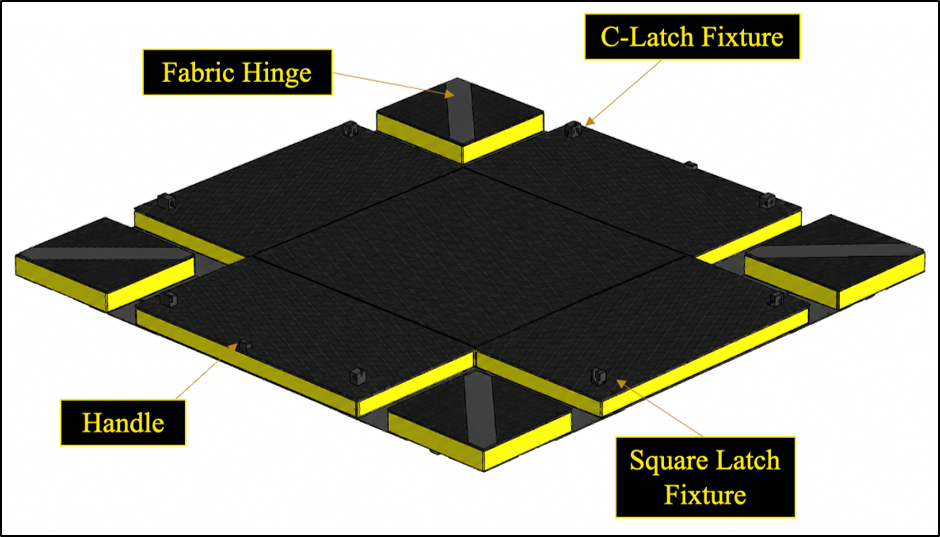
\includegraphics[
        width=1.92in,
        height=1.30in,
        keepaspectratio
    ]{toro_cover_underside_cad}
};
\draw[RuleGray,line width=0.55pt,rounded corners=4pt]
    ($(current page.north west)+(2.62in,-5.04in)$)
    rectangle
    ($(current page.north west)+(4.70in,-6.43in)$);

% Image 3: folded CAD
\node[anchor=center,inner sep=0pt]
at ($(current page.north west)+(5.85in,-5.73in)$)
{
    \includegraphics[
        width=1.92in,
        height=1.30in,
        keepaspectratio
    ]{\detokenize{Toro_Cover_folded Configuration}}
};
\draw[RuleGray,line width=0.55pt,rounded corners=4pt]
    ($(current page.north west)+(4.81in,-5.04in)$)
    rectangle
    ($(current page.north west)+(6.89in,-6.43in)$);

% Image 4: dual-use product concept
\node[anchor=center,inner sep=0pt]
at ($(current page.north west)+(8.04in,-5.73in)$)
{
    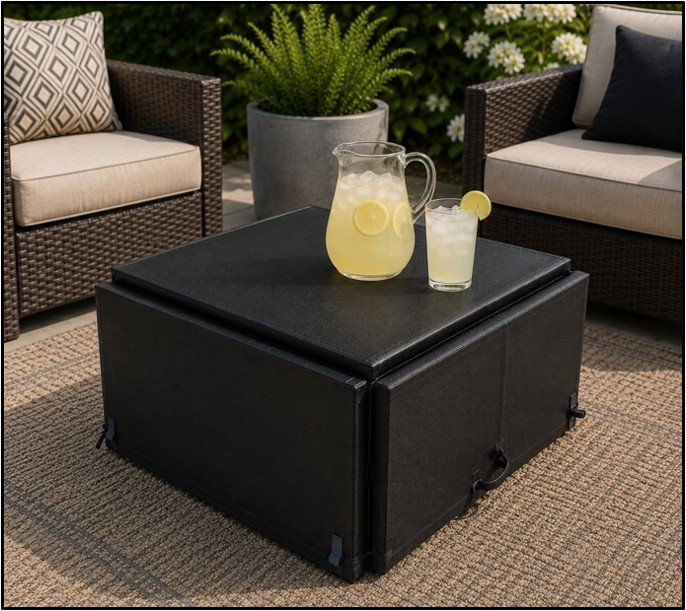
\includegraphics[
        width=1.92in,
        height=1.30in,
        keepaspectratio
    ]{generative_AI_concept_toro_cover_art}
};
\draw[RuleGray,line width=0.55pt,rounded corners=4pt]
    ($(current page.north west)+(7.00in,-5.04in)$)
    rectangle
    ($(current page.north west)+(9.08in,-6.43in)$);

% Image 5: folded foam functional prototype
% The portrait photograph is deliberately clipped to the landscape frame
% so the ottoman fills the card without extending beyond its border.
\begin{scope}
\clip[rounded corners=4pt]
    ($(current page.north west)+(9.19in,-5.04in)$)
    rectangle
    ($(current page.north east)+(-0.43in,-6.43in)$);

% Keep the original image proportions and center it within the existing card.
\node[anchor=center,inner sep=0pt]
at ($(current page.north west)+(9.88in,-5.735in)$)
{
    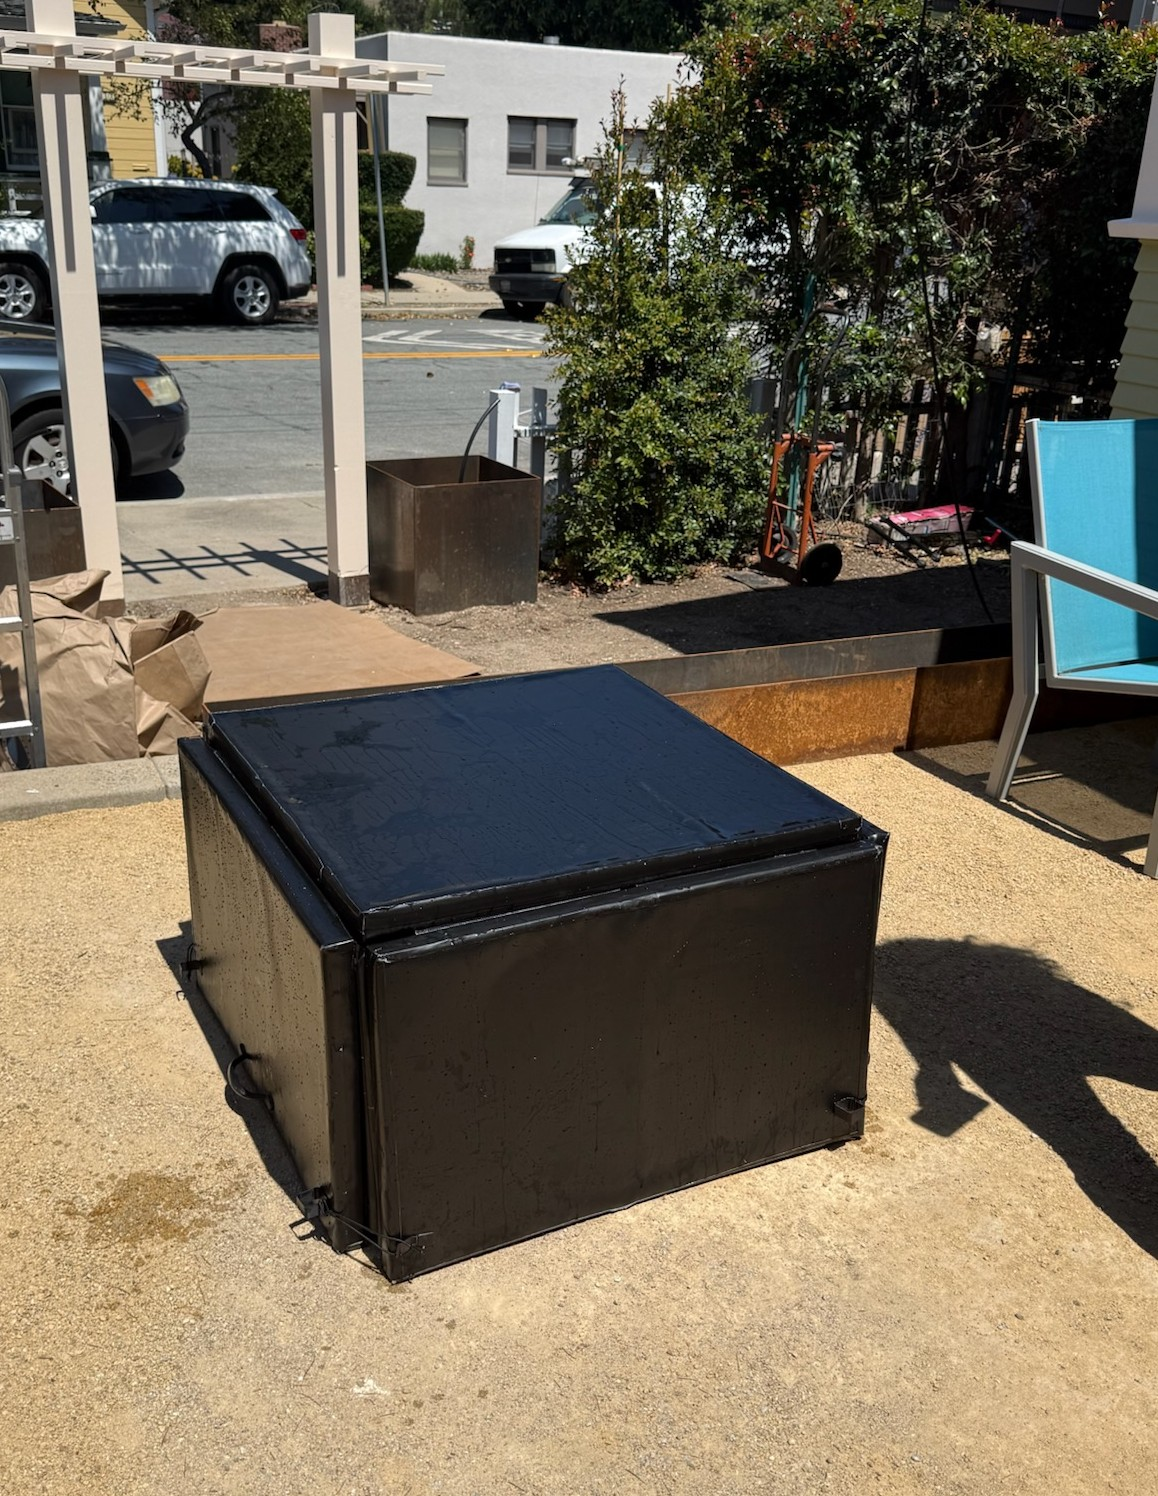
\includegraphics[
        width=1.58in,
        height=1.28in,
        keepaspectratio
    ]{foam_model_folded_backyard_image}
};
\end{scope}

\draw[RuleGray,line width=0.55pt,rounded corners=4pt]
    ($(current page.north west)+(9.19in,-5.04in)$)
    rectangle
    ($(current page.north east)+(-0.43in,-6.43in)$);

% Larger captions
\node[anchor=north,align=center,text width=1.95in,text=Muted,
      font=\sffamily\fontsize{6.8}{7.4}\selectfont]
at ($(current page.north west)+(1.47in,-6.49in)$)
{Topside panel architecture};

\node[anchor=north,align=center,text width=1.95in,text=Muted,
      font=\sffamily\fontsize{6.8}{7.4}\selectfont]
at ($(current page.north west)+(3.66in,-6.49in)$)
{Underside hinge architecture};

\node[anchor=north,align=center,text width=1.95in,text=Muted,
      font=\sffamily\fontsize{6.8}{7.4}\selectfont]
at ($(current page.north west)+(5.85in,-6.49in)$)
{Folded CAD configuration};

\node[anchor=north,align=center,text width=1.95in,text=Muted,
      font=\sffamily\fontsize{6.8}{7.4}\selectfont]
at ($(current page.north west)+(8.04in,-6.49in)$)
{Dual-use product vision};

\node[anchor=north,align=center,text width=1.95in,text=Muted,
      font=\sffamily\fontsize{6.8}{7.4}\selectfont]
at ($(current page.north west)+(9.88in,-6.49in)$)
{Folded foam prototype};

% Page 1 resource bar — centered and non-repeated resources
\fill[Panel,rounded corners=4pt]
    ($(current page.north west)+(0.43in,-7.05in)$)
    rectangle
    ($(current page.north east)+(-0.43in,-7.64in)$);
\draw[RuleGray,line width=0.5pt,rounded corners=4pt]
    ($(current page.north west)+(0.43in,-7.05in)$)
    rectangle
    ($(current page.north east)+(-0.43in,-7.64in)$);

\node[
    anchor=center,
    align=center,
    text=DeepGreen,
    font=\sffamily\bfseries\fontsize{6.9}{7.5}\selectfont
]
at ($(current page.north)+(0,-7.345in)$)
{\href{\ToroDrawingLink}{\faDraftingCompass\ DRAWING PACKAGE}
\hspace{24pt}
\href{\ToroDimensionsLink}{\faImage\ DIMENSION STUDY}
\hspace{24pt}
\href{\ToroProblemLink}{\faFileImage\ PROBLEM STATEMENT}};

% Footer
\node[
    anchor=south west,
    text=white,
    font=\sffamily\bfseries\fontsize{7.1}{7.7}\selectfont
]
at ($(current page.south west)+(0.42in,0.17in)$)
{\hyperlink{composites}{\faArrowLeft\ COMPOSITES}};

\node[
    anchor=south,
    text=white,
    font=\sffamily\fontsize{7.0}{7.6}\selectfont
]
at ($(current page.south)+(0,0.17in)$)
{TORO COVER \hspace{6pt} 1 / 3};

\node[
    anchor=south east,
    text=white,
    font=\sffamily\bfseries\fontsize{7.1}{7.7}\selectfont
]
at ($(current page.south east)+(-0.42in,0.17in)$)
{MANUFACTURING-DRIVEN DESIGN \faArrowRight};

\end{tikzpicture}


% ============================================================
% PAGE 2 — MANUFACTURING-DRIVEN DESIGN
% ============================================================

\clearpage
\thispagestyle{empty}
\hypertarget{toro-manufacturing}{}
\null

\begin{tikzpicture}[remember picture,overlay]

% Background and bars
\fill[white]
    (current page.south west)
    rectangle
    (current page.north east);

\fill[DeepGreen]
    (current page.north west)
    rectangle
    ($(current page.north east)+(0,-0.095in)$);

\fill[PolyGold]
    ($(current page.north west)+(0,-0.095in)$)
    rectangle
    ($(current page.north east)+(0,-0.14in)$);

\fill[DeepGreen]
    (current page.south west)
    rectangle
    ($(current page.south east)+(0,0.36in)$);

\fill[PolyGold]
    ($(current page.south west)+(0,0.36in)$)
    rectangle
    ($(current page.south east)+(0,0.405in)$);

% Header
\node[
    anchor=north west,
    text=PolyGold,
    font=\sffamily\bfseries\fontsize{8.1}{8.7}\selectfont
]
at ($(current page.north west)+(0.42in,-0.39in)$)
{TORO COVER \hspace{5pt}/\hspace{5pt} DESIGN FOR MANUFACTURABILITY};

\node[
    anchor=north west,
    text=DeepGreen,
    font=\bfseries\fontsize{23}{24}\selectfont
]
at ($(current page.north west)+(0.40in,-0.67in)$)
{THE ENVELOPE METHOD};

\node[
    anchor=north west,
    text=Muted,
    font=\sffamily\fontsize{8.7}{9.6}\selectfont
]
at ($(current page.north west)+(0.42in,-1.12in)$)
{A one-layup process developed for unusually thick insulated composite sandwich panels};

\fill[PolyGold]
    ($(current page.north west)+(0.42in,-1.36in)$)
    rectangle
    ($(current page.north west)+(5.30in,-1.315in)$);

% Process explanation
\fill[SoftGold,rounded corners=5pt]
    ($(current page.north west)+(0.42in,-1.61in)$)
    rectangle
    ($(current page.north east)+(-0.42in,-2.90in)$);

\fill[PolyGold]
    ($(current page.north west)+(0.42in,-1.61in)$)
    rectangle
    ($(current page.north west)+(0.52in,-2.90in)$);

\node[
    anchor=north west,
    text=DeepGreen,
    font=\sffamily\bfseries\fontsize{7.9}{8.6}\selectfont
]
at ($(current page.north west)+(0.67in,-1.76in)$)
{PROCESS INNOVATION};

\node[
    anchor=north west,
    align=left,
    text width=9.55in,
    text=Ink,
    font=\fontsize{7.35}{8.75}\selectfont
]
at ($(current page.north west)+(0.67in,-2.02in)$)
{
Weight reduction and insulation were both essential, leading to the selection of an
XPS foam core. Because XPS could not tolerate composite heat-cure temperatures, prepreg
processing was not practical and the panels had to be manufactured by wet layup with a
room-temperature cure. To simplify this process, I waterjet-cut XPS perimeter strips from
excess foam and placed them around each core inside the vacuum enclosure. Under vacuum,
the top and bottom carbon skins met along the panel sides and compressed against this
border, eliminating a separate edge-banding layup and reducing corner pleating.
};

% Workflow title
\node[
    anchor=north west,
    text=DeepGreen,
    font=\sffamily\bfseries\fontsize{8.0}{8.7}\selectfont
]
at ($(current page.north west)+(0.43in,-3.06in)$)
{MANUFACTURING WORKFLOW};

% Row 1 image 1
\node[anchor=center,inner sep=0pt]
at ($(current page.north west)+(2.07in,-4.105in)$)
{
    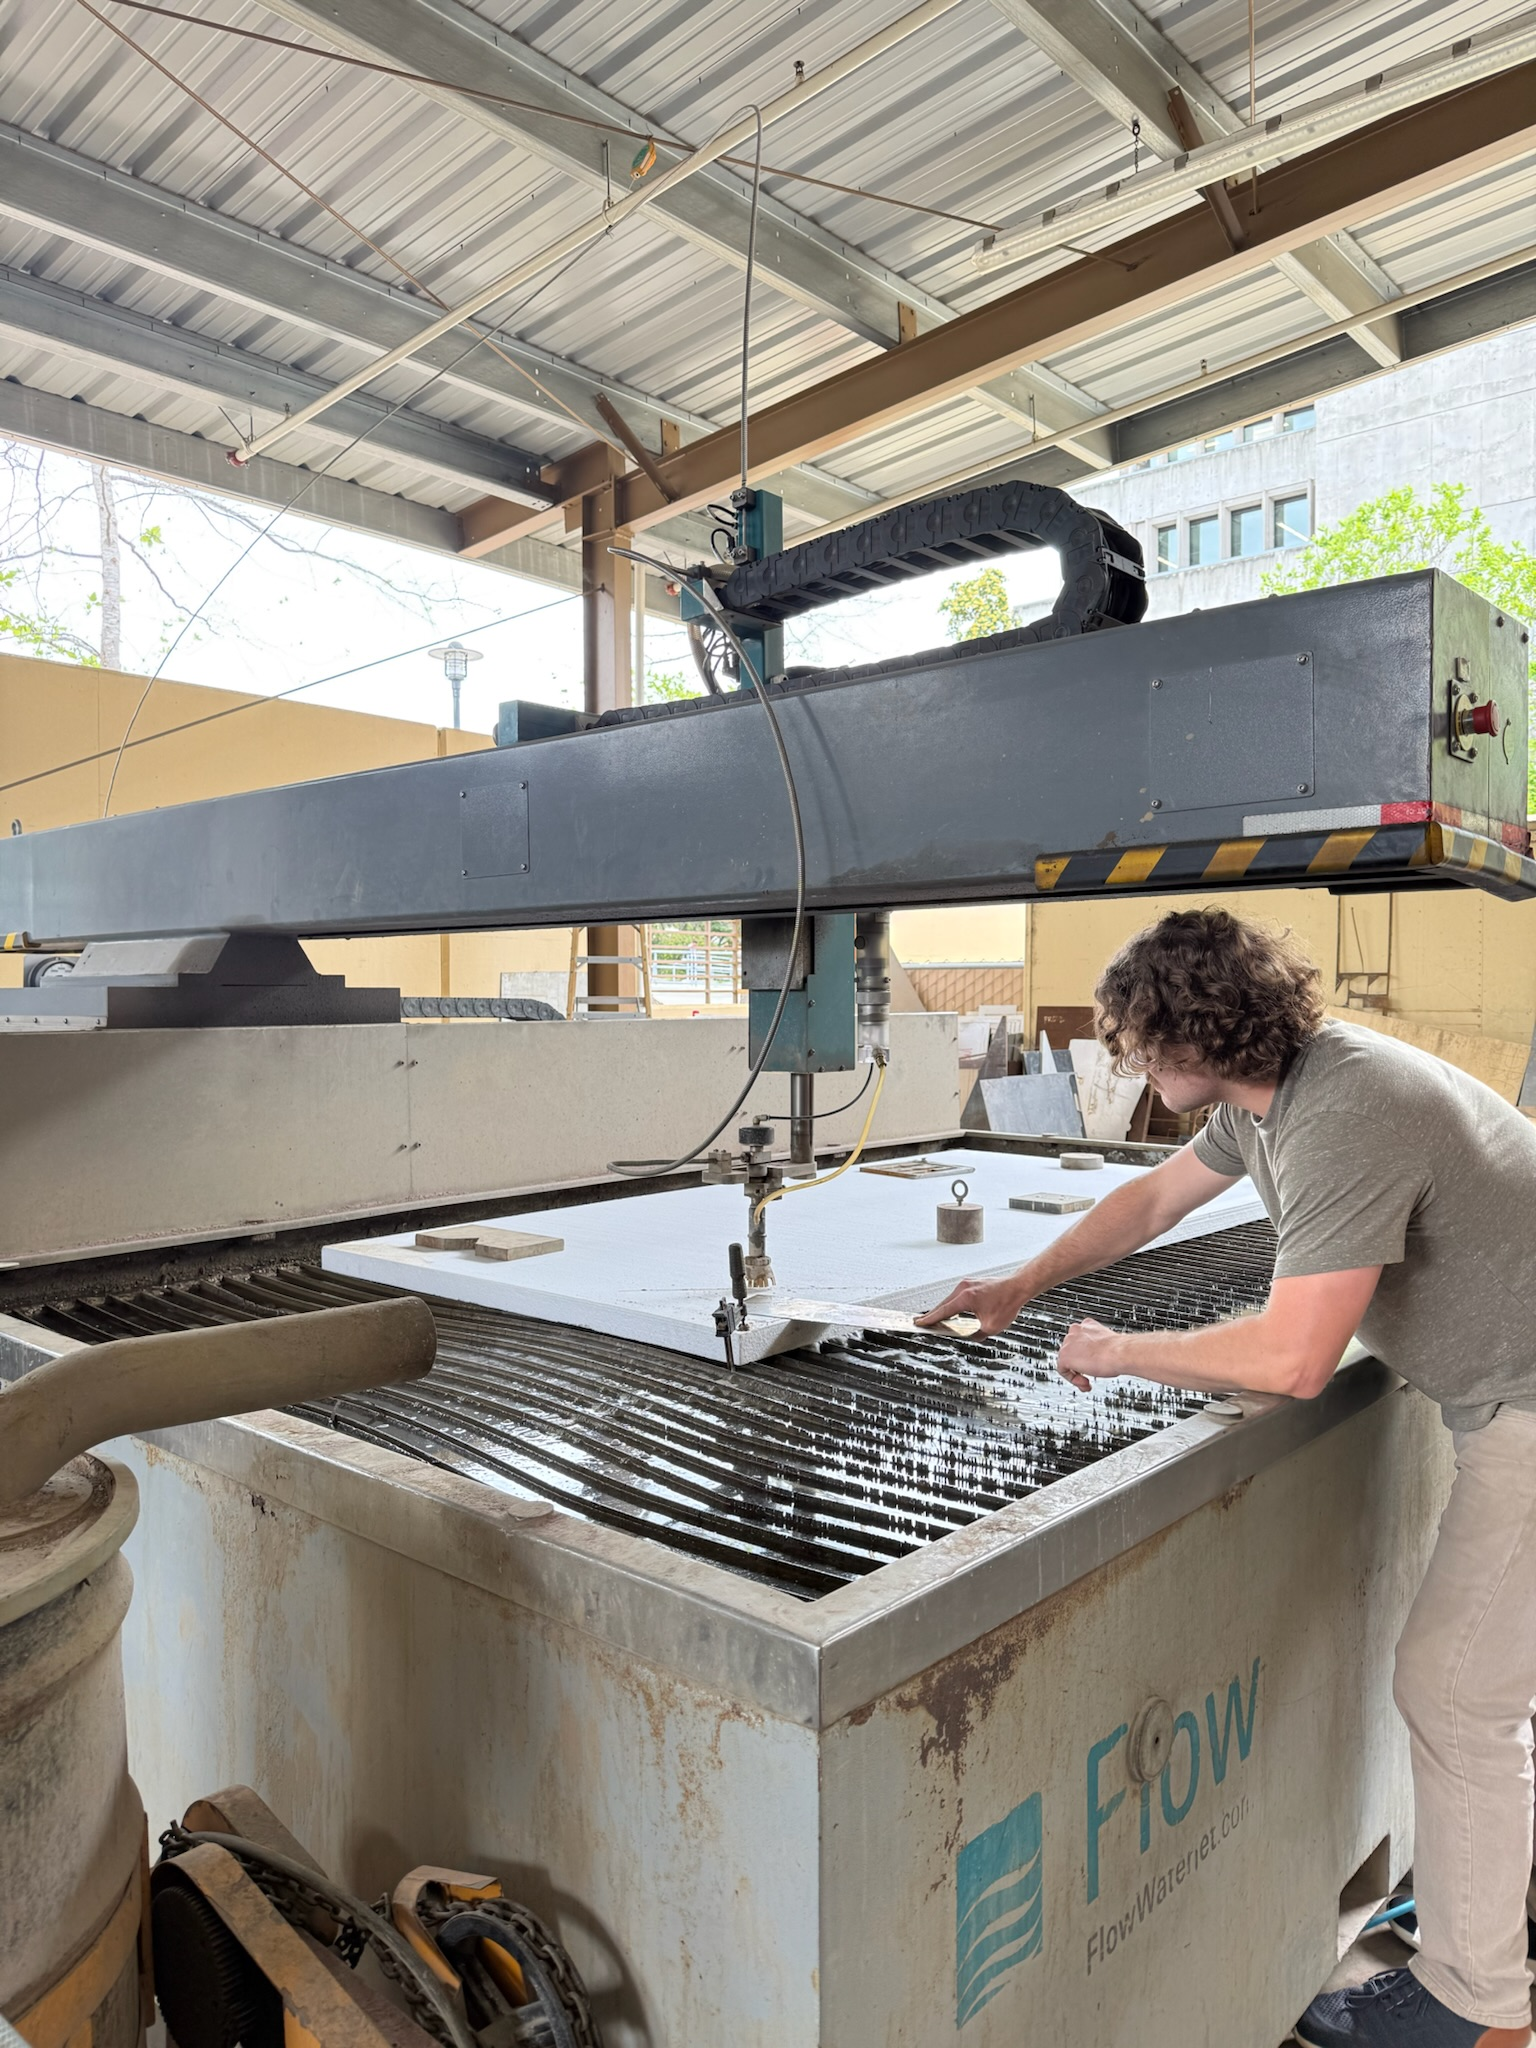
\includegraphics[
        width=3.10in,
        height=1.40in,
        keepaspectratio
    ]{waterjet_foam}
};
\draw[RuleGray,line width=0.55pt,rounded corners=4pt]
    ($(current page.north west)+(0.43in,-3.36in)$)
    rectangle
    ($(current page.north west)+(3.71in,-4.85in)$);

% Row 1 image 2
\node[anchor=center,inner sep=0pt]
at ($(current page.north west)+(5.50in,-4.105in)$)
{
    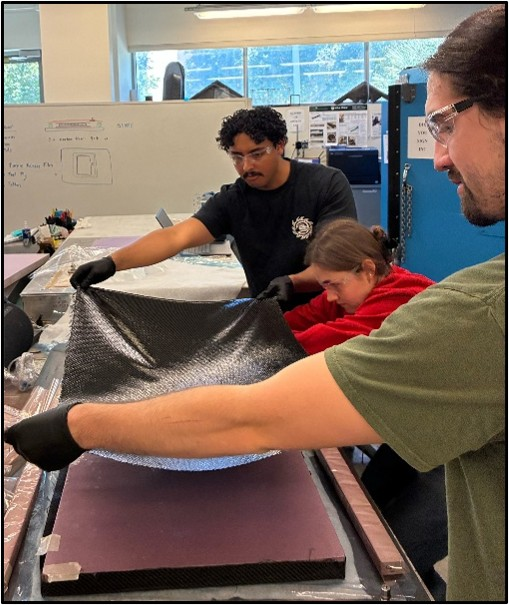
\includegraphics[
        width=3.10in,
        height=1.40in,
        keepaspectratio
    ]{group_layup}
};
\draw[RuleGray,line width=0.55pt,rounded corners=4pt]
    ($(current page.north west)+(3.86in,-3.36in)$)
    rectangle
    ($(current page.north west)+(7.14in,-4.85in)$);

% Row 1 image 3
\node[anchor=center,inner sep=0pt]
at ($(current page.north west)+(8.935in,-4.105in)$)
{
    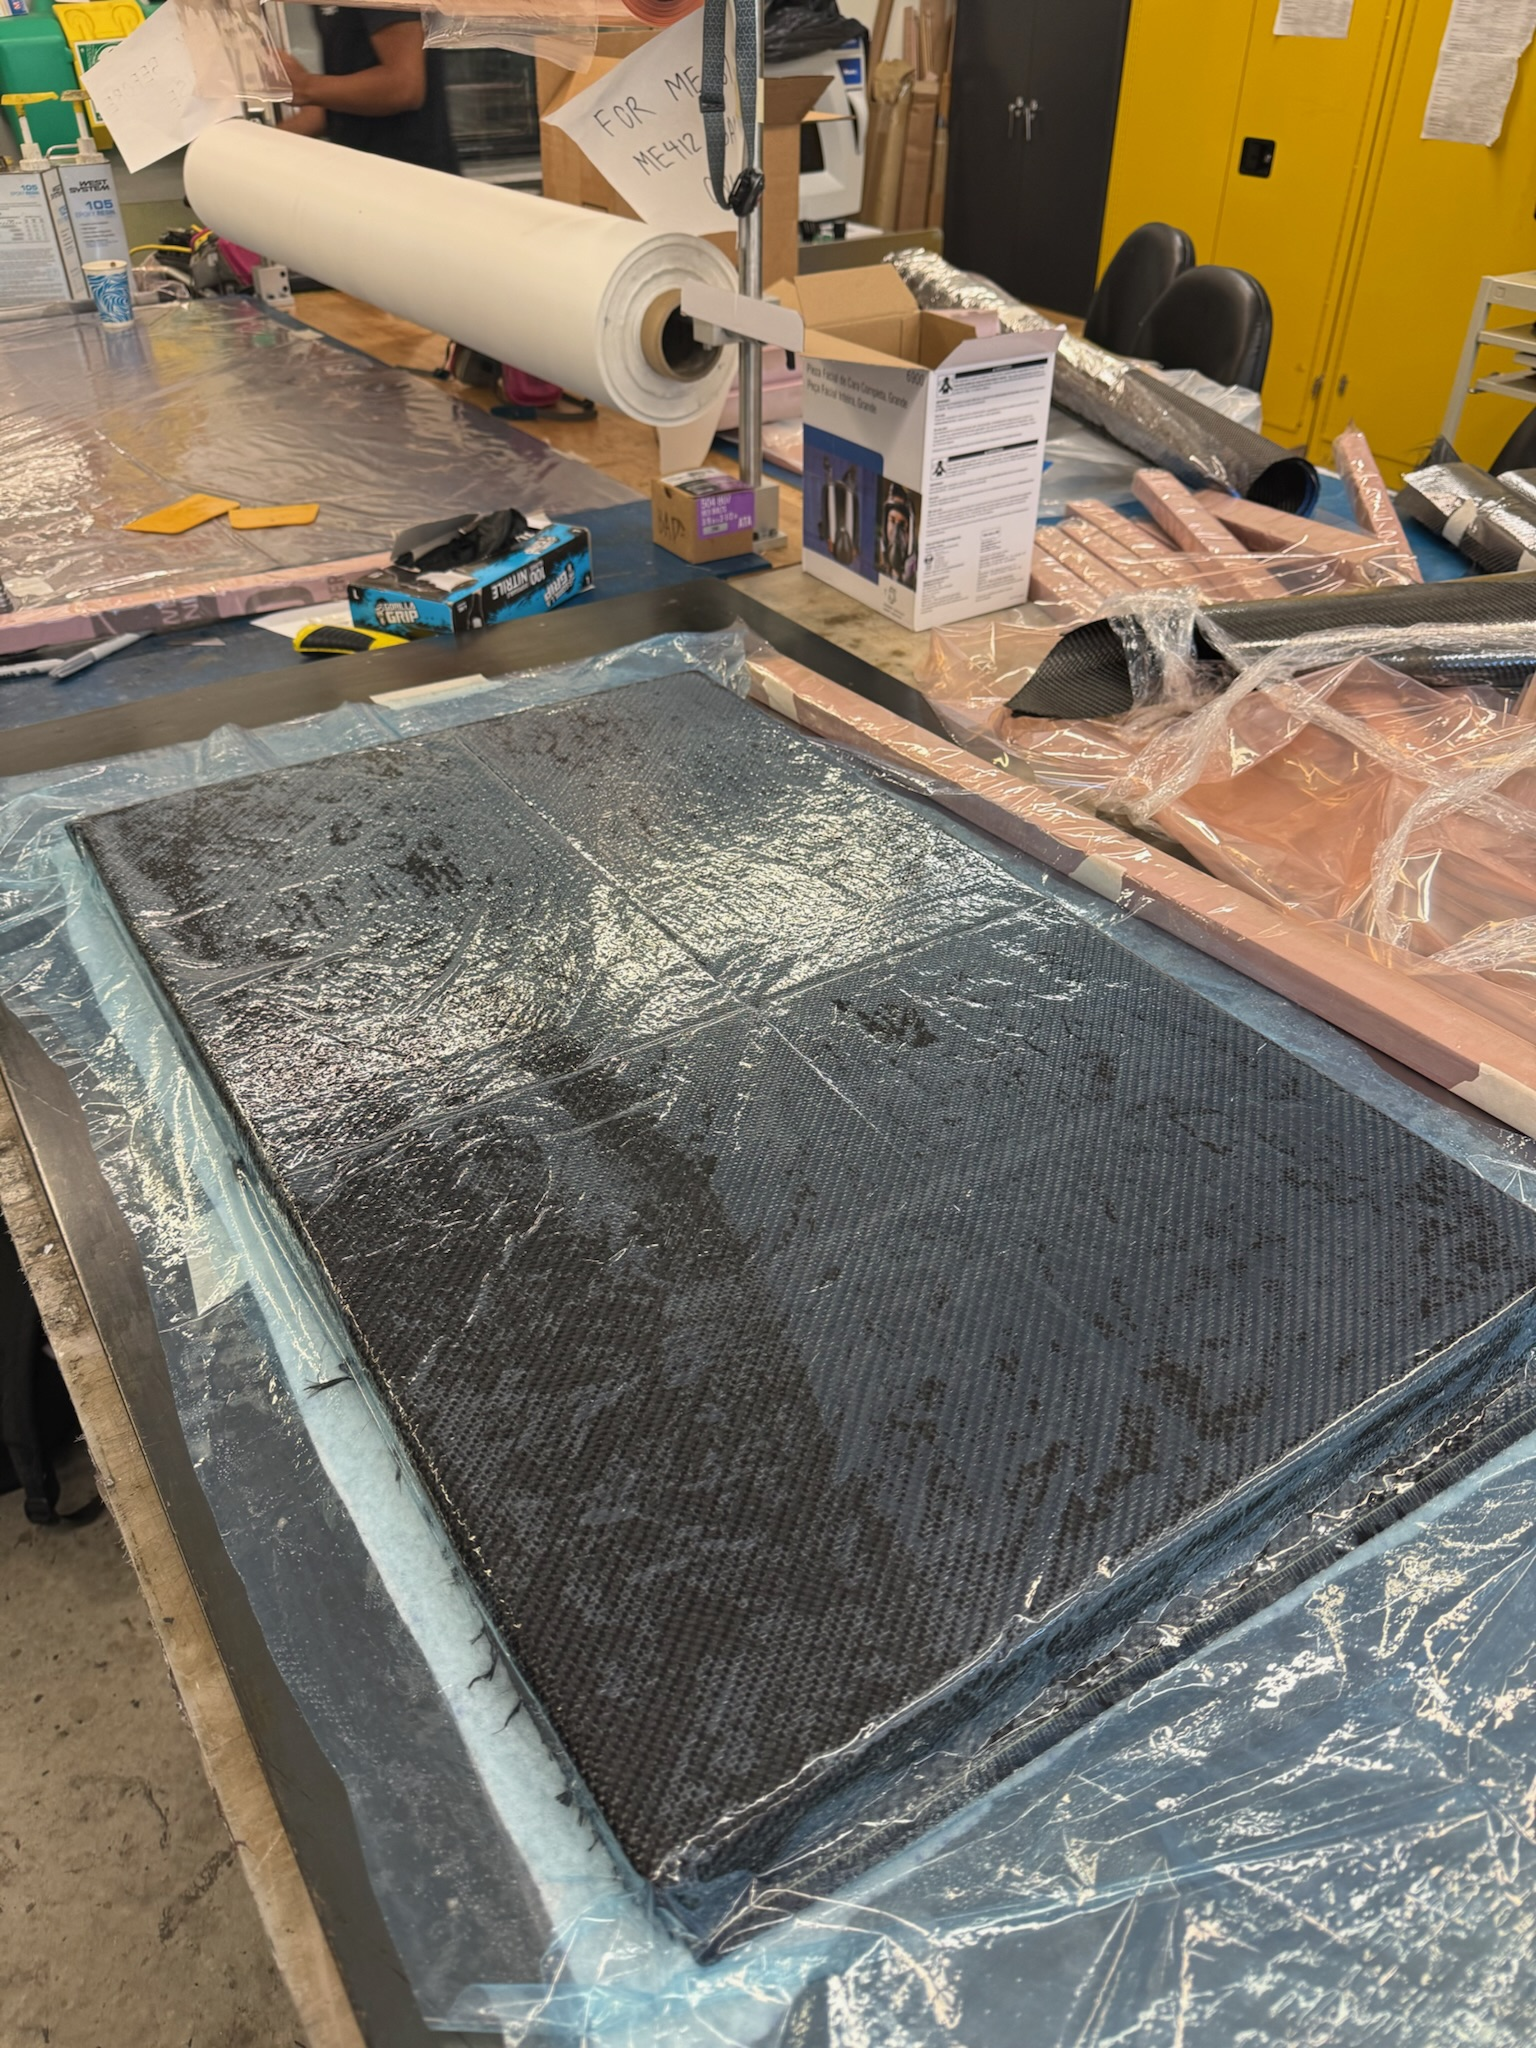
\includegraphics[
        width=3.10in,
        height=1.40in,
        keepaspectratio
    ]{blue_perforrated_film_layup}
};
\draw[RuleGray,line width=0.55pt,rounded corners=4pt]
    ($(current page.north west)+(7.29in,-3.36in)$)
    rectangle
    ($(current page.north east)+(-0.42in,-4.85in)$);

% Row 1 captions
\node[anchor=north,text=Muted,font=\sffamily\fontsize{6.7}{7.3}\selectfont]
at ($(current page.north west)+(2.07in,-4.90in)$)
{1. Waterjet-cut core and perimeter geometry};

\node[anchor=north,text=Muted,font=\sffamily\fontsize{6.7}{7.3}\selectfont]
at ($(current page.north west)+(5.50in,-4.90in)$)
{2. Team wet layup under my process guidance};

\node[anchor=north,text=Muted,font=\sffamily\fontsize{6.7}{7.3}\selectfont]
at ($(current page.north west)+(8.935in,-4.90in)$)
{3. Perforated film, breather, and vacuum enclosure};

% Row 2 image 1
\node[anchor=center,inner sep=0pt]
at ($(current page.north west)+(2.07in,-5.875in)$)
{
    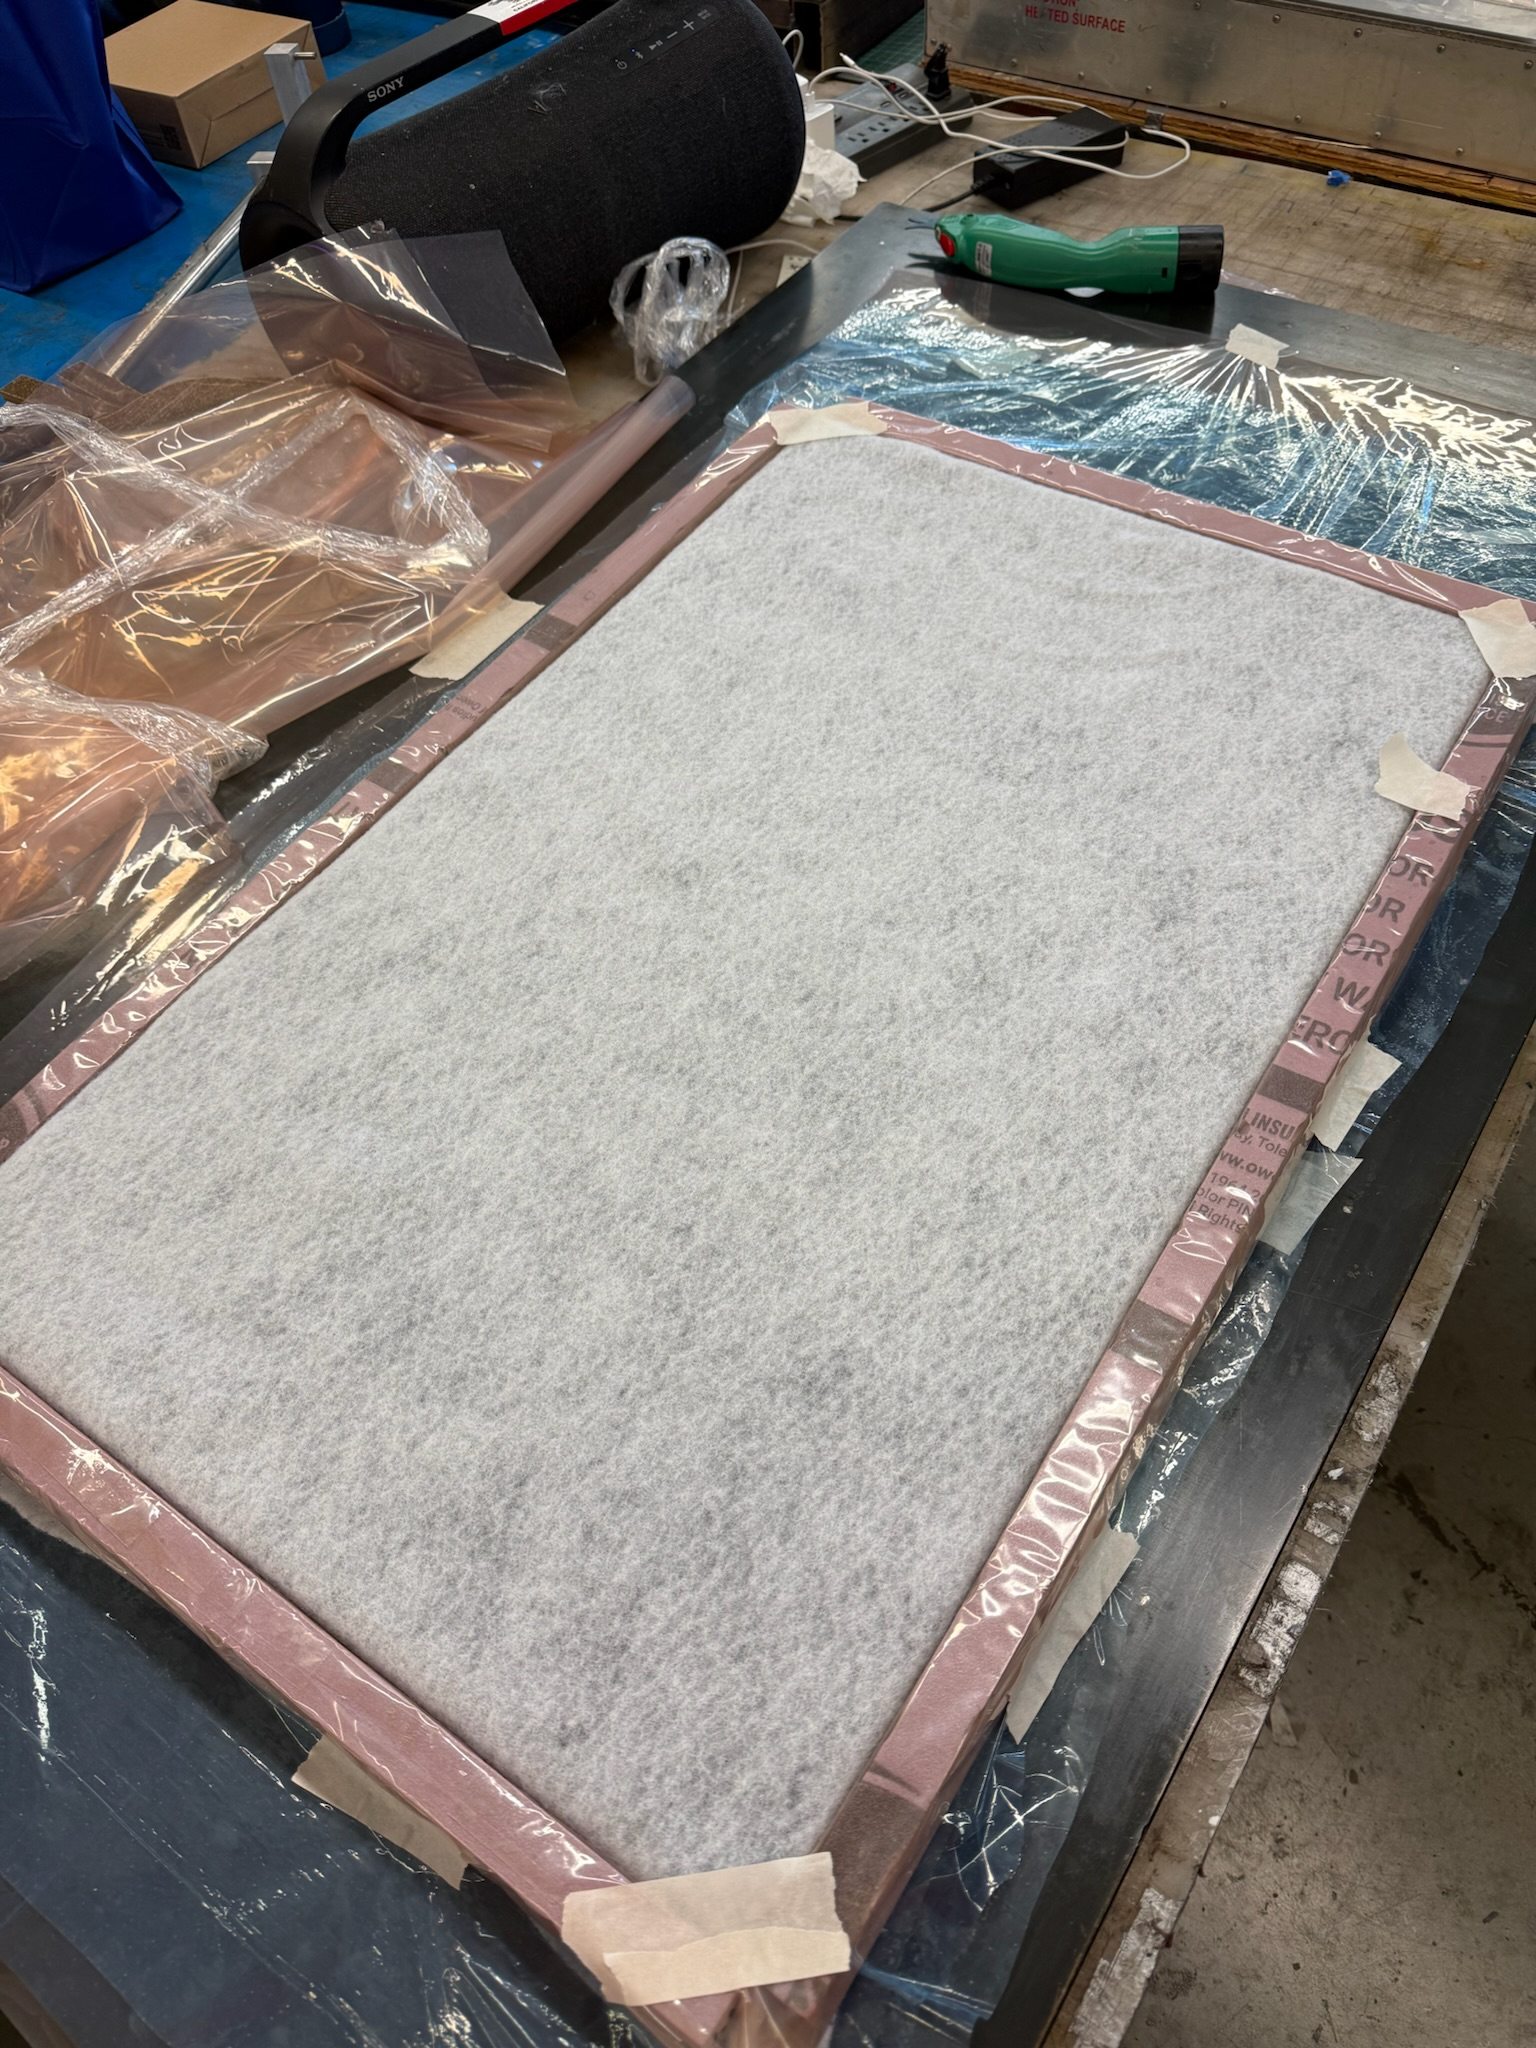
\includegraphics[
        width=3.10in,
        height=1.40in,
        keepaspectratio
    ]{completed_layup}
};
\draw[RuleGray,line width=0.55pt,rounded corners=4pt]
    ($(current page.north west)+(0.43in,-5.13in)$)
    rectangle
    ($(current page.north west)+(3.71in,-6.62in)$);

% Row 2 image 2 — oven chamber used only as a reliable vacuum enclosure; no heat applied
\node[anchor=center,inner sep=0pt]
at ($(current page.north west)+(5.50in,-5.875in)$)
{
    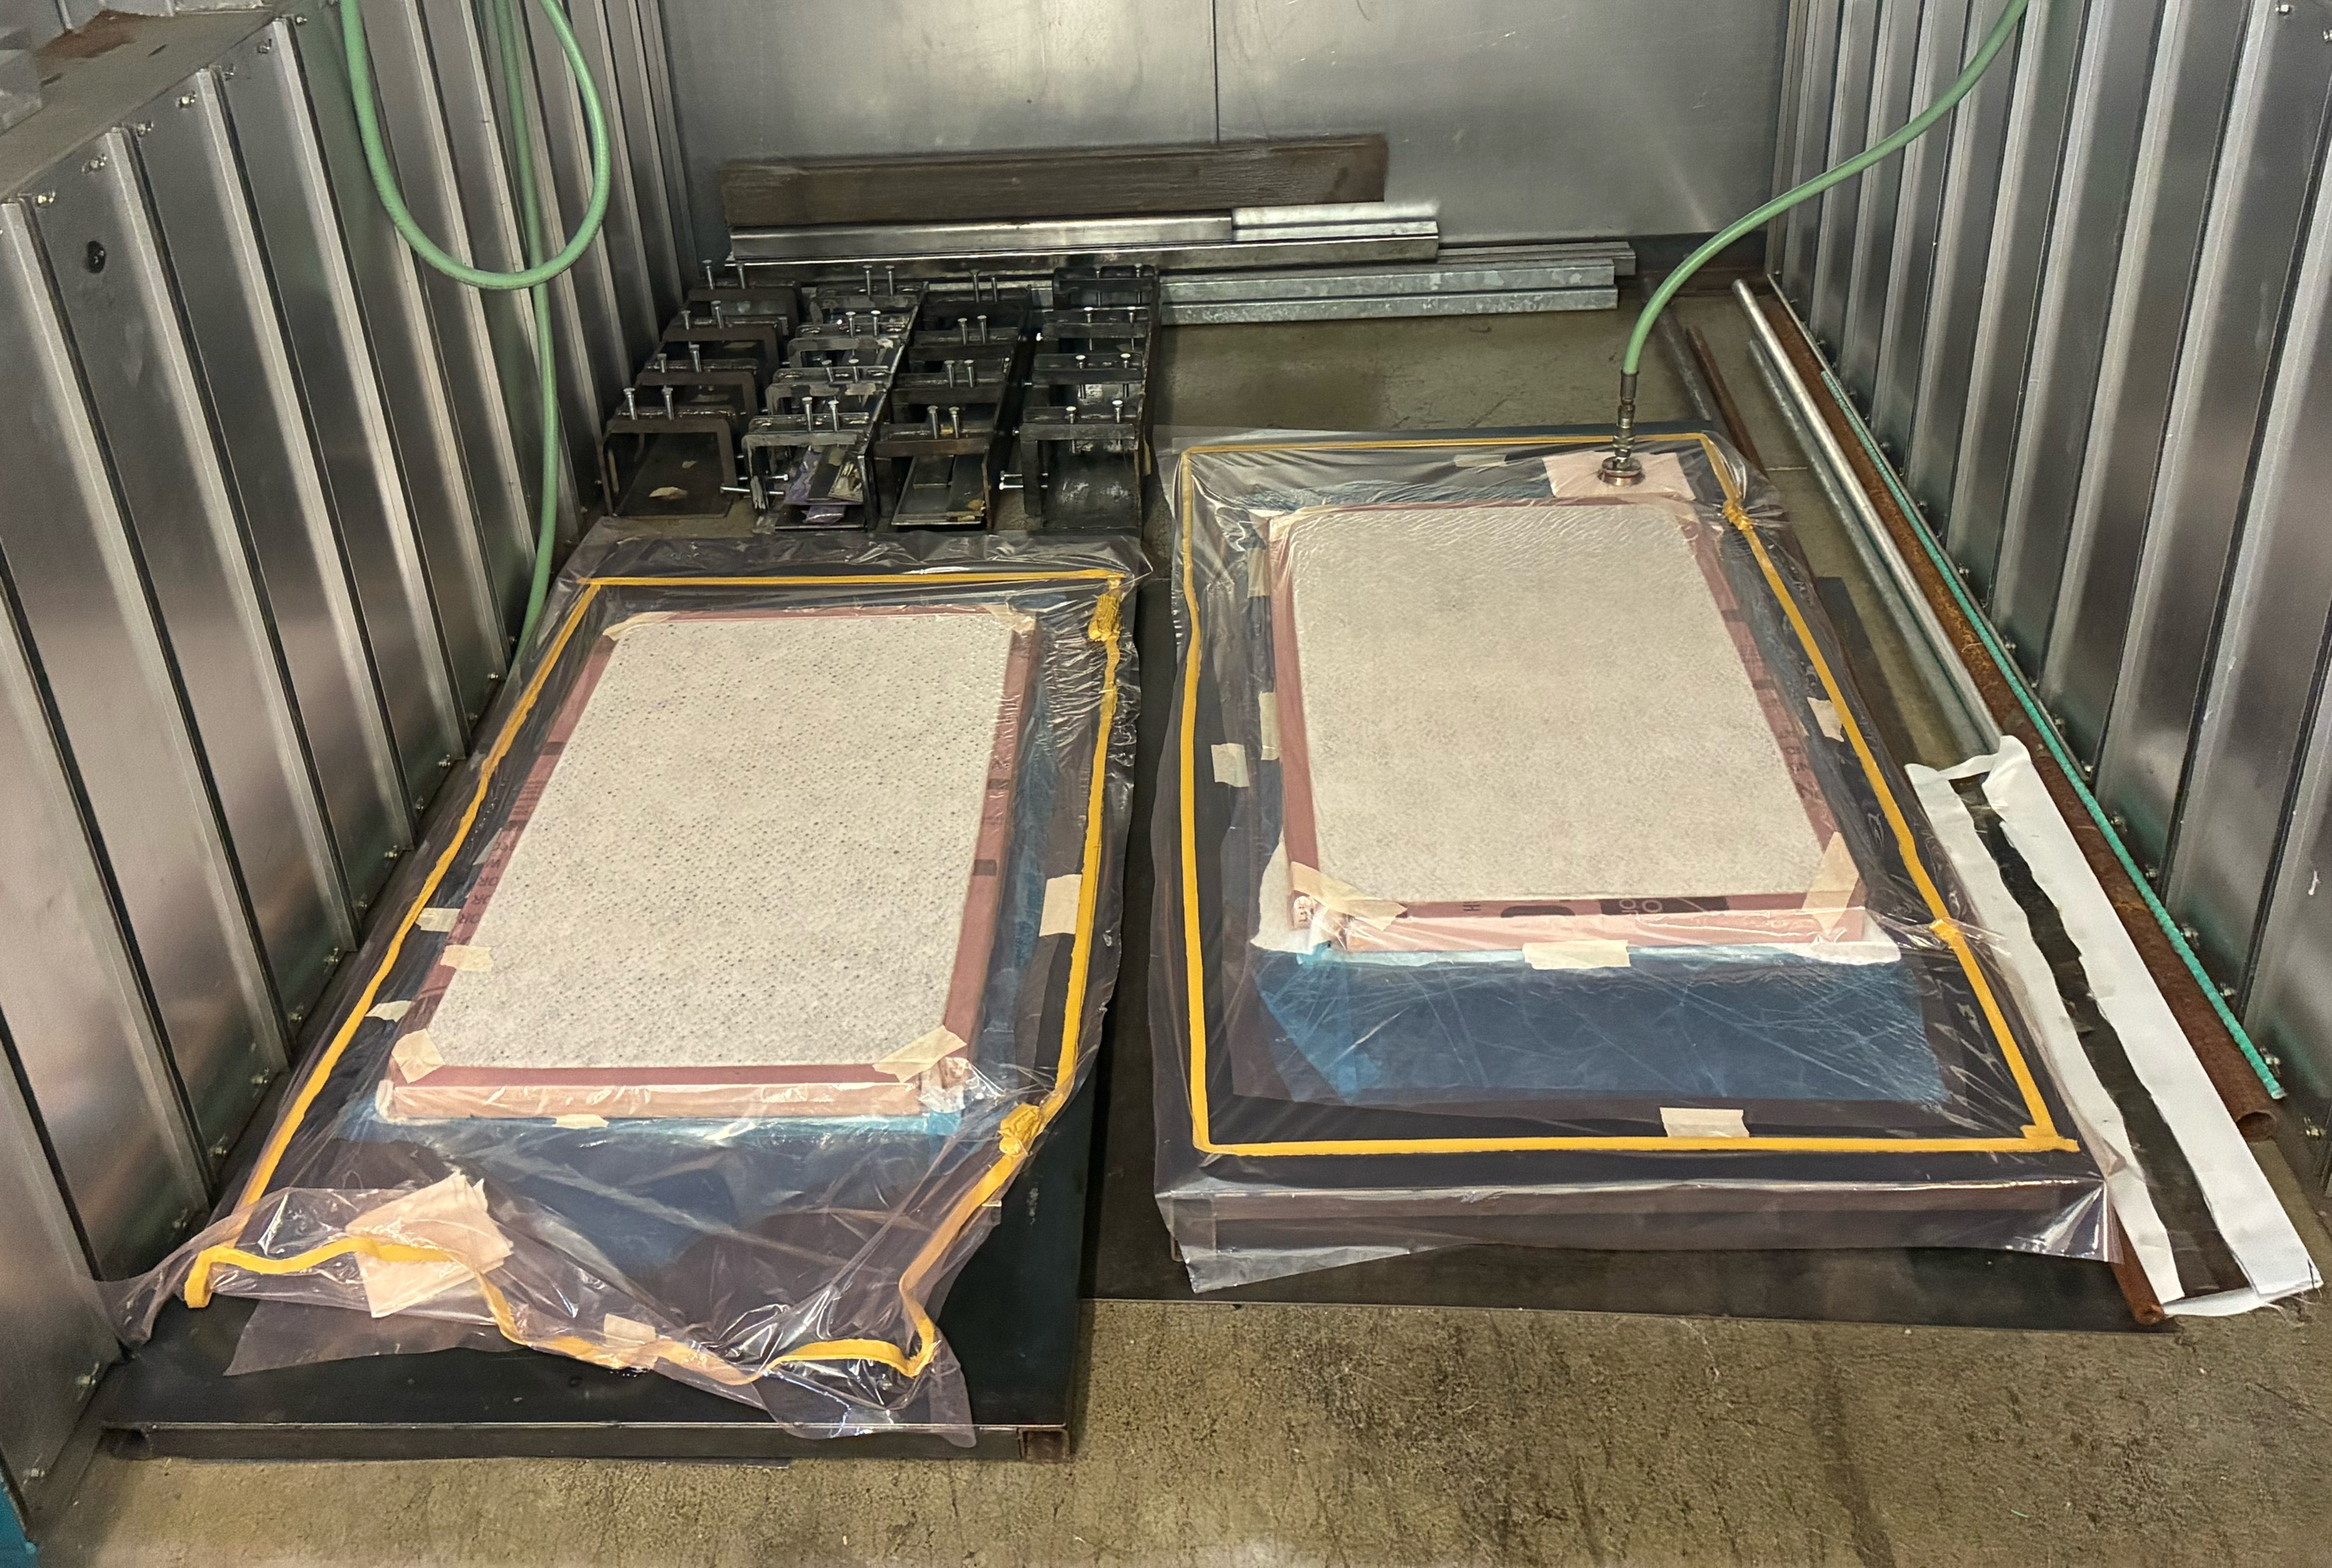
\includegraphics[
        width=3.10in,
        height=1.40in,
        keepaspectratio
    ]{layups_in_composite_oven_under_vacuumPressure}
};
\draw[RuleGray,line width=0.55pt,rounded corners=4pt]
    ($(current page.north west)+(3.86in,-5.13in)$)
    rectangle
    ($(current page.north west)+(7.14in,-6.62in)$);

% Row 2 image 3
\node[anchor=center,inner sep=0pt]
at ($(current page.north west)+(8.935in,-5.875in)$)
{
    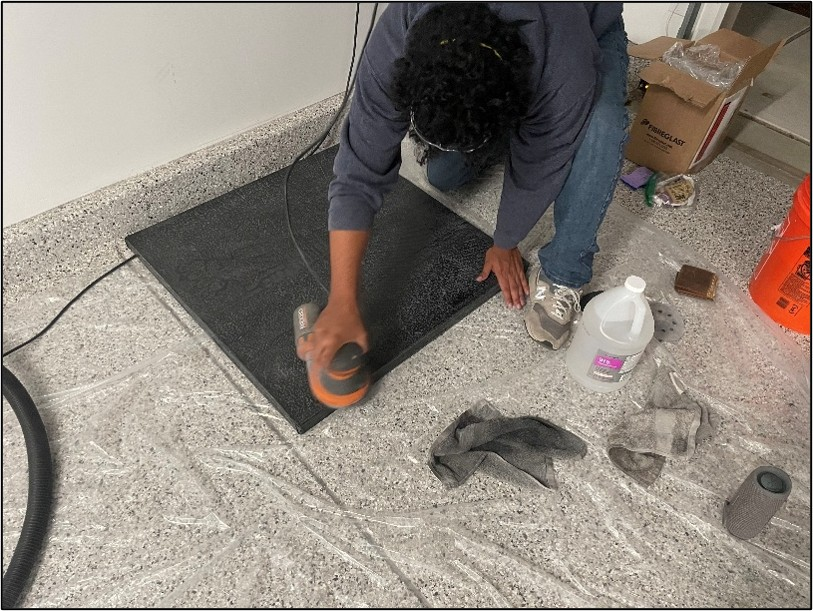
\includegraphics[
        width=3.10in,
        height=1.40in,
        keepaspectratio
    ]{garage_sanding}
};
\draw[RuleGray,line width=0.55pt,rounded corners=4pt]
    ($(current page.north west)+(7.29in,-5.13in)$)
    rectangle
    ($(current page.north east)+(-0.42in,-6.62in)$);

% Row 2 captions
\node[anchor=north,text=Muted,font=\sffamily\fontsize{6.7}{7.3}\selectfont]
at ($(current page.north west)+(2.07in,-6.67in)$)
{4. Fully saturated carbon skin and foam sandwich};

\node[anchor=north,text=Muted,font=\sffamily\fontsize{6.7}{7.3}\selectfont]
at ($(current page.north west)+(5.50in,-6.67in)$)
{5. Room-temperature cure under continuous vacuum};

\node[anchor=north,text=Muted,font=\sffamily\fontsize{6.7}{7.3}\selectfont]
at ($(current page.north west)+(8.935in,-6.67in)$)
{6. Post-processing and surface preparation};

% Bottom callouts
\fill[Panel,rounded corners=4pt]
    ($(current page.north west)+(0.43in,-6.95in)$)
    rectangle
    ($(current page.north west)+(5.48in,-7.60in)$);

\draw[RuleGray,line width=0.55pt,rounded corners=4pt]
    ($(current page.north west)+(0.43in,-6.95in)$)
    rectangle
    ($(current page.north west)+(5.48in,-7.60in)$);

\node[
    anchor=north west,
    text=DeepGreen,
    font=\sffamily\bfseries\fontsize{7.0}{7.6}\selectfont
]
at ($(current page.north west)+(0.63in,-7.08in)$)
{FROM THREE LAYUPS TO ONE};

\node[
    anchor=north west,
    align=left,
    text width=4.56in,
    text=Ink,
    font=\fontsize{6.45}{7.45}\selectfont
]
at ($(current page.north west)+(0.63in,-7.29in)$)
{
The Envelope Method reduced labor, cure cycles, handling,
alignment risk, and time spent forming numerous vacuum-bag
pleats around the 1.5-inch-thick XPS panels.
};

\fill[Panel,rounded corners=4pt]
    ($(current page.north west)+(5.68in,-6.95in)$)
    rectangle
    ($(current page.north east)+(-0.42in,-7.60in)$);

\draw[RuleGray,line width=0.55pt,rounded corners=4pt]
    ($(current page.north west)+(5.68in,-6.95in)$)
    rectangle
    ($(current page.north east)+(-0.42in,-7.60in)$);

\node[
    anchor=north west,
    text=DeepGreen,
    font=\sffamily\bfseries\fontsize{7.0}{7.6}\selectfont
]
at ($(current page.north west)+(5.88in,-7.08in)$)
{WHY SURFACE-BONDED HARDWARE};

\node[
    anchor=north west,
    align=left,
    text width=4.55in,
    text=Ink,
    font=\fontsize{6.45}{7.45}\selectfont
]
at ($(current page.north west)+(5.88in,-7.29in)$)
{
Adhesively bonded hinges and fixtures preserved the clean
composite exterior and avoided drilled inserts, foam-core
crushing, added stress concentrations, and new leak paths.
};


% Footer
\node[
    anchor=south west,
    text=white,
    font=\sffamily\bfseries\fontsize{7.1}{7.7}\selectfont
]
at ($(current page.south west)+(0.42in,0.17in)$)
{\faArrowLeft\ PRODUCT ARCHITECTURE};

\node[
    anchor=south,
    text=white,
    font=\sffamily\fontsize{7.0}{7.6}\selectfont
]
at ($(current page.south)+(0,0.17in)$)
{TORO COVER \hspace{6pt} 2 / 3};

\node[
    anchor=south east,
    text=white,
    font=\sffamily\bfseries\fontsize{7.1}{7.7}\selectfont
]
at ($(current page.south east)+(-0.42in,0.17in)$)
{VALIDATION \& TAKEAWAYS \faArrowRight};

\end{tikzpicture}


% ============================================================
% PAGE 3 — FINISHING, VALIDATION, AND TAKEAWAYS
% ============================================================

\clearpage
\thispagestyle{empty}
\hypertarget{toro-results}{}
\null

\begin{tikzpicture}[remember picture,overlay]

% Background and bars
\fill[white]
    (current page.south west)
    rectangle
    (current page.north east);

\fill[DeepGreen]
    (current page.north west)
    rectangle
    ($(current page.north east)+(0,-0.095in)$);

\fill[PolyGold]
    ($(current page.north west)+(0,-0.095in)$)
    rectangle
    ($(current page.north east)+(0,-0.14in)$);

\fill[DeepGreen]
    (current page.south west)
    rectangle
    ($(current page.south east)+(0,0.36in)$);

\fill[PolyGold]
    ($(current page.south west)+(0,0.36in)$)
    rectangle
    ($(current page.south east)+(0,0.405in)$);

% Header
\node[
    anchor=north west,
    text=PolyGold,
    font=\sffamily\bfseries\fontsize{8.1}{8.7}\selectfont
]
at ($(current page.north west)+(0.42in,-0.39in)$)
{TORO COVER \hspace{5pt}/\hspace{5pt} VALIDATION AND ENGINEERING TAKEAWAYS};

\node[
    anchor=north west,
    text=DeepGreen,
    font=\bfseries\fontsize{22.5}{23.5}\selectfont
]
at ($(current page.north west)+(0.40in,-0.67in)$)
{FROM PROTOTYPE TO PRODUCT PATHWAY};

\node[
    anchor=north west,
    text=Muted,
    font=\sffamily\fontsize{8.7}{9.6}\selectfont
]
at ($(current page.north west)+(0.42in,-1.12in)$)
{Environmental protection, usability testing, scope decisions, and lessons from technical leadership};

\fill[PolyGold]
    ($(current page.north west)+(0.42in,-1.36in)$)
    rectangle
    ($(current page.north west)+(5.8in,-1.315in)$);

% Finishing title
\node[
    anchor=north west,
    text=DeepGreen,
    font=\sffamily\bfseries\fontsize{8.0}{8.7}\selectfont
]
at ($(current page.north west)+(0.43in,-1.62in)$)
{OUTDOOR FINISHING AND ENVIRONMENTAL PROTECTION};

% Image 1
\node[anchor=center,inner sep=0pt]
at ($(current page.north west)+(1.705in,-2.655in)$)
{
    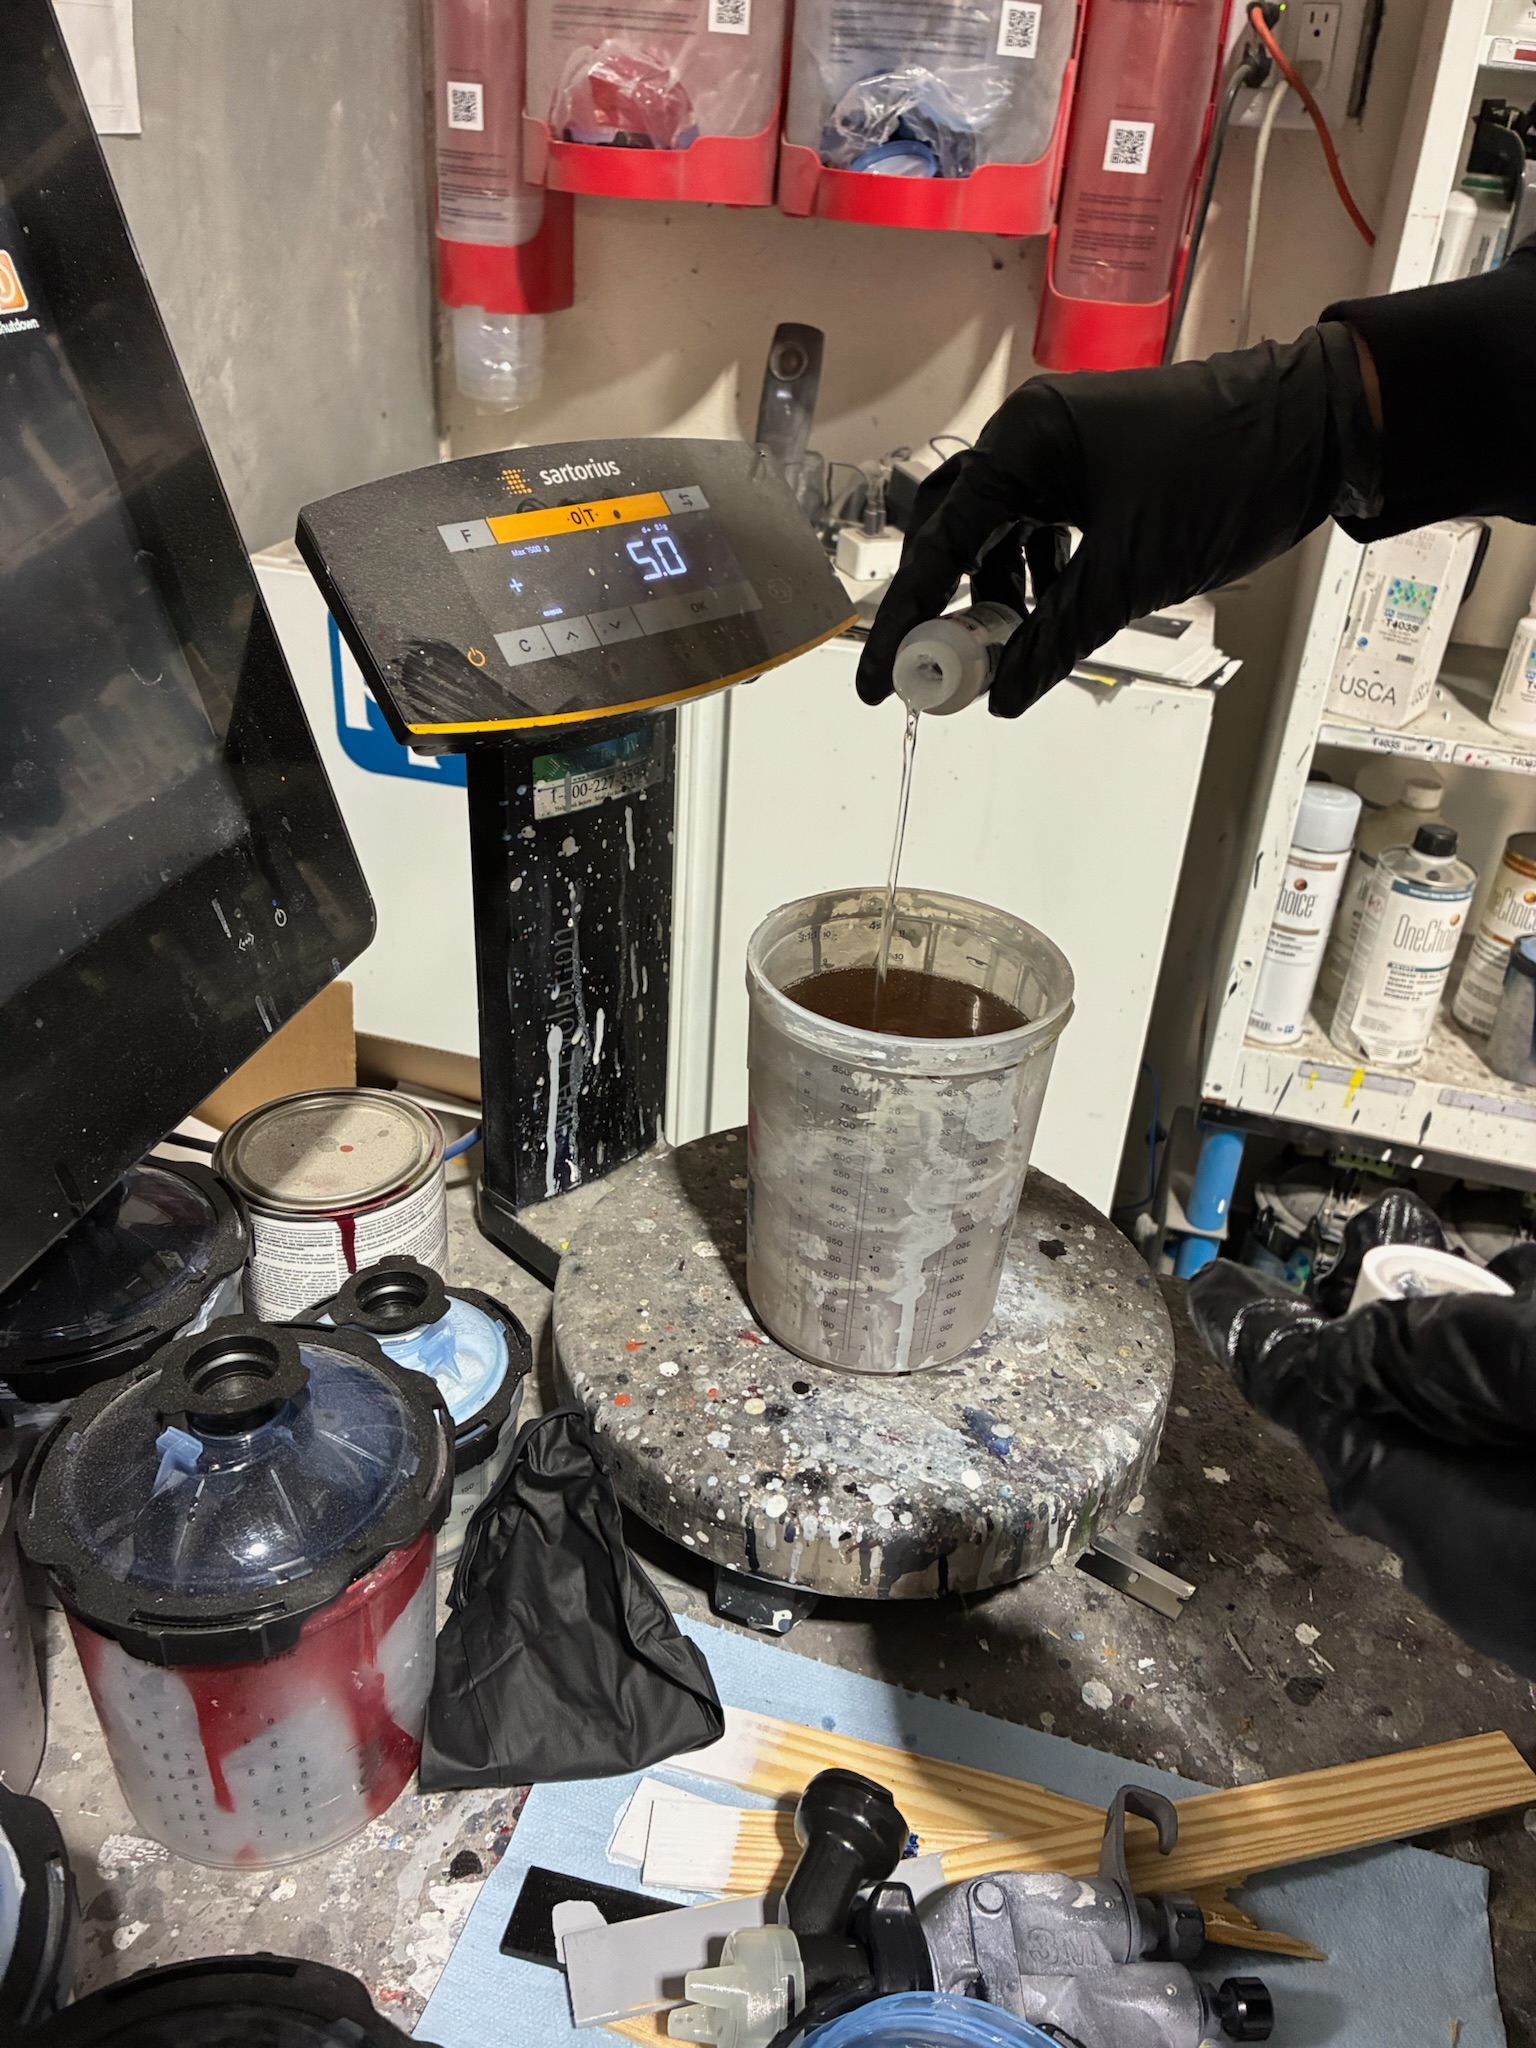
\includegraphics[
        width=2.35in,
        height=1.40in,
        keepaspectratio
    ]{spray_topcoat_prep}
};
\draw[RuleGray,line width=0.55pt,rounded corners=4pt]
    ($(current page.north west)+(0.43in,-1.91in)$)
    rectangle
    ($(current page.north west)+(2.98in,-3.40in)$);

% Image 2
\node[anchor=center,inner sep=0pt]
at ($(current page.north west)+(4.375in,-2.655in)$)
{
    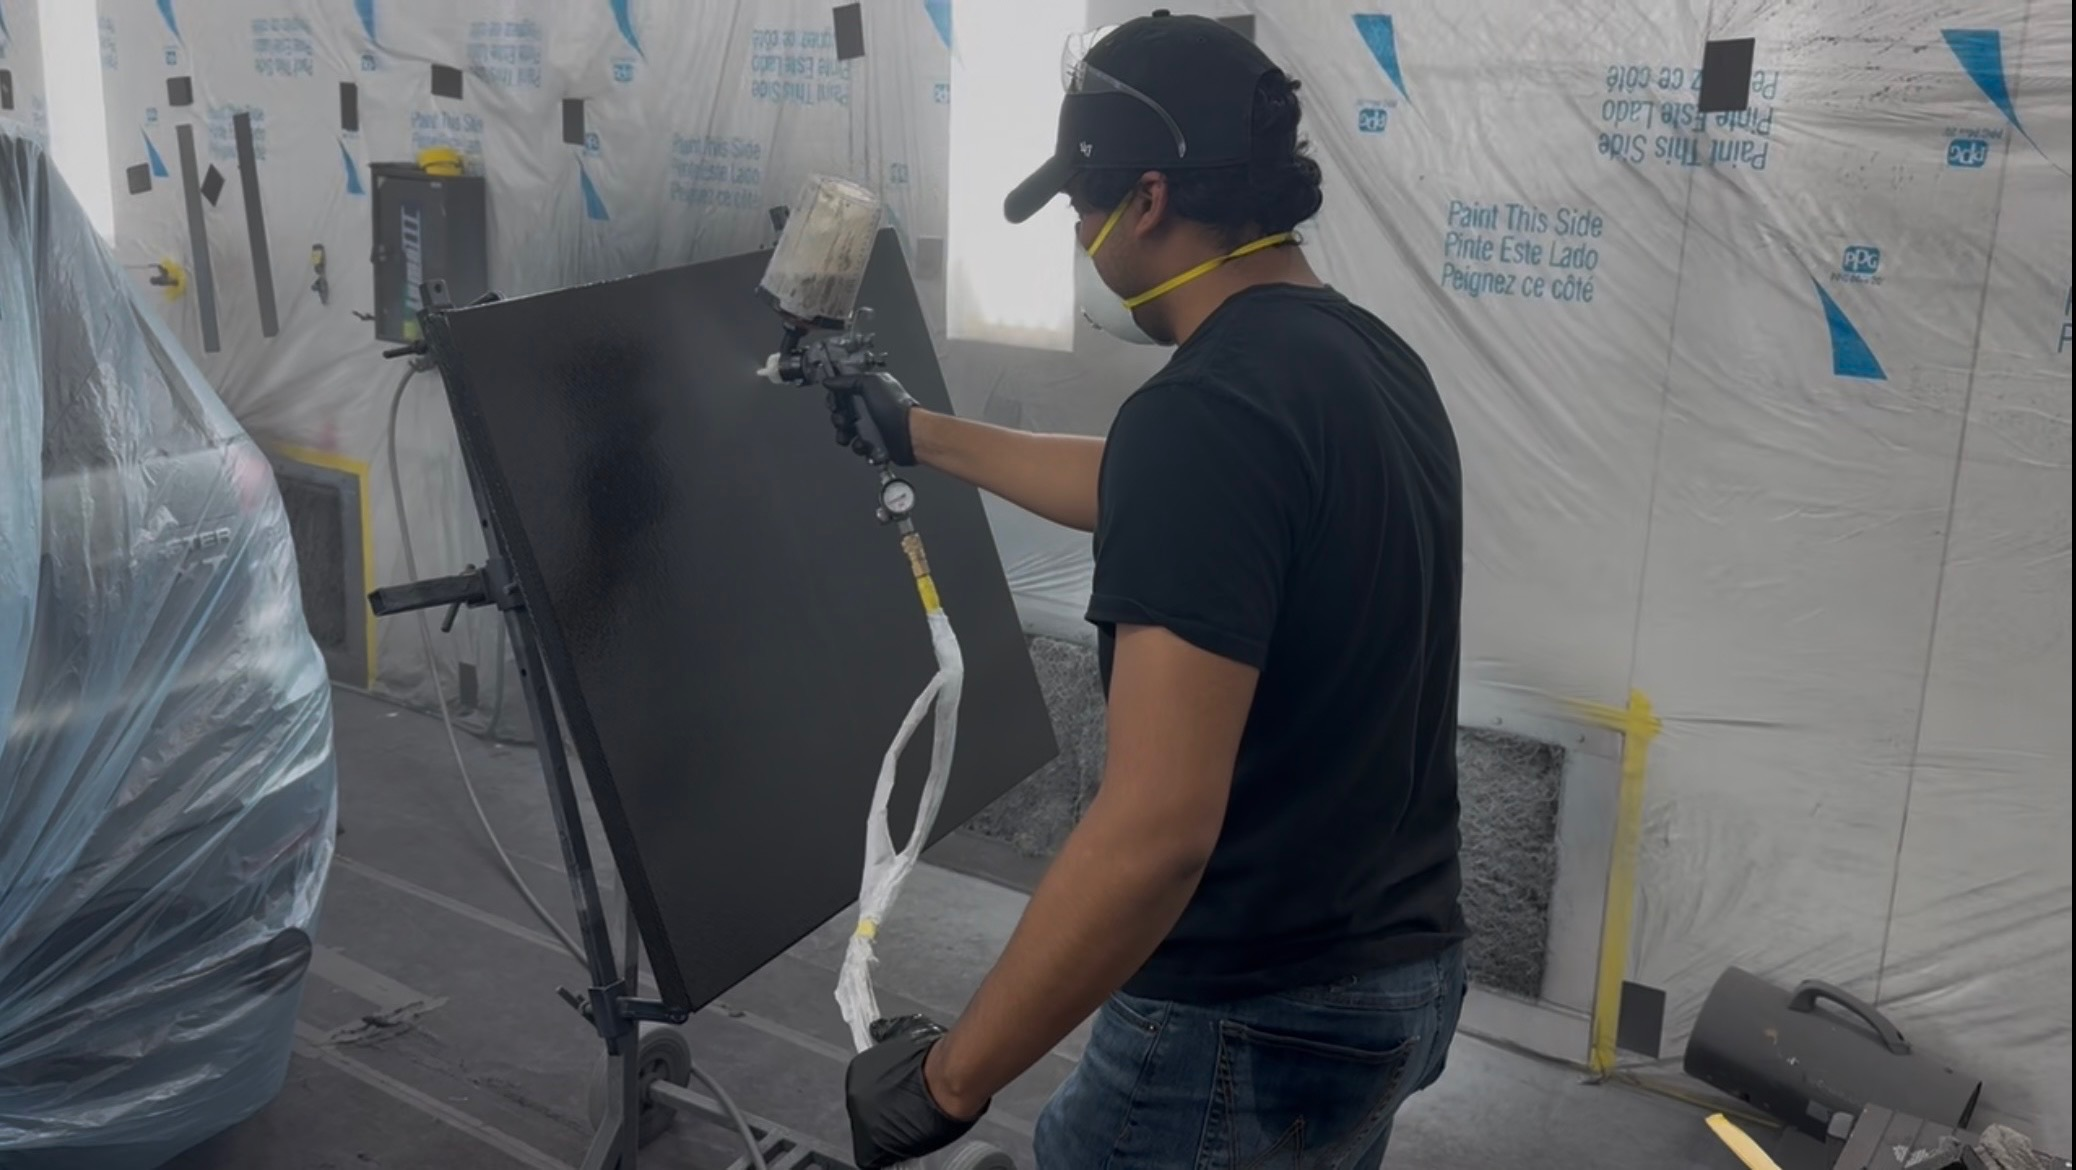
\includegraphics[
        width=2.35in,
        height=1.40in,
        keepaspectratio
    ]{spraying_topcoat}
};
\draw[RuleGray,line width=0.55pt,rounded corners=4pt]
    ($(current page.north west)+(3.10in,-1.91in)$)
    rectangle
    ($(current page.north west)+(5.65in,-3.40in)$);

% Image 3
\node[anchor=center,inner sep=0pt]
at ($(current page.north west)+(7.045in,-2.655in)$)
{
    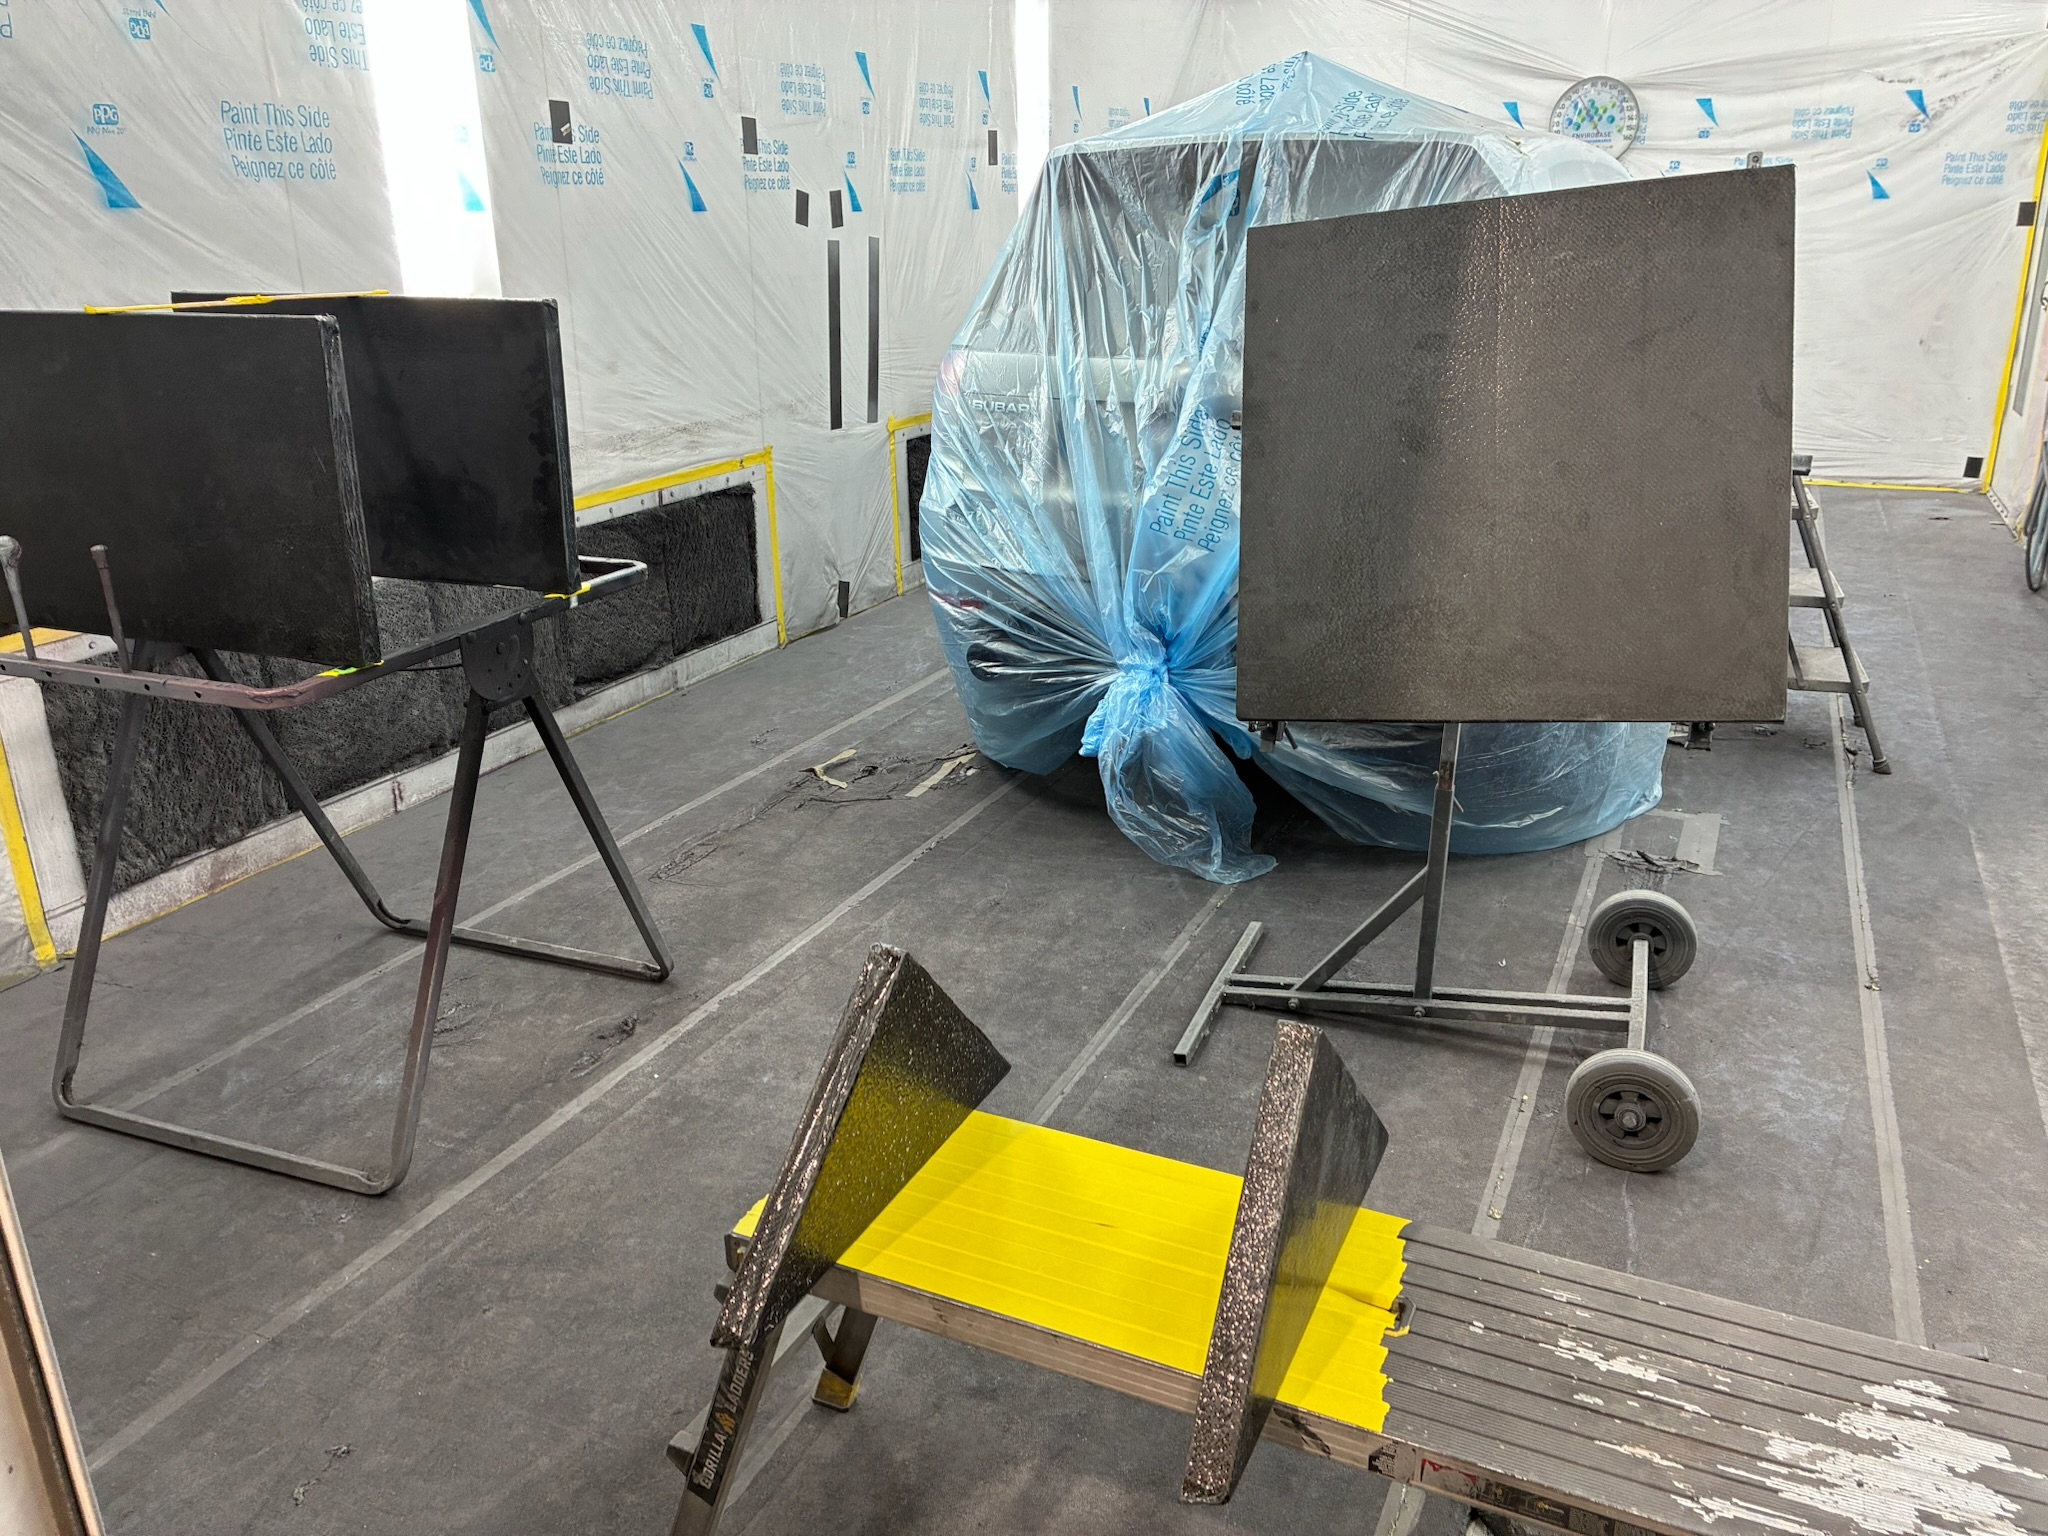
\includegraphics[
        width=2.35in,
        height=1.40in,
        keepaspectratio
    ]{topcoat_setup_apparatus}
};
\draw[RuleGray,line width=0.55pt,rounded corners=4pt]
    ($(current page.north west)+(5.77in,-1.91in)$)
    rectangle
    ($(current page.north west)+(8.32in,-3.40in)$);

% Image 4
\node[anchor=center,inner sep=0pt]
at ($(current page.north west)+(9.50in,-2.655in)$)
{
    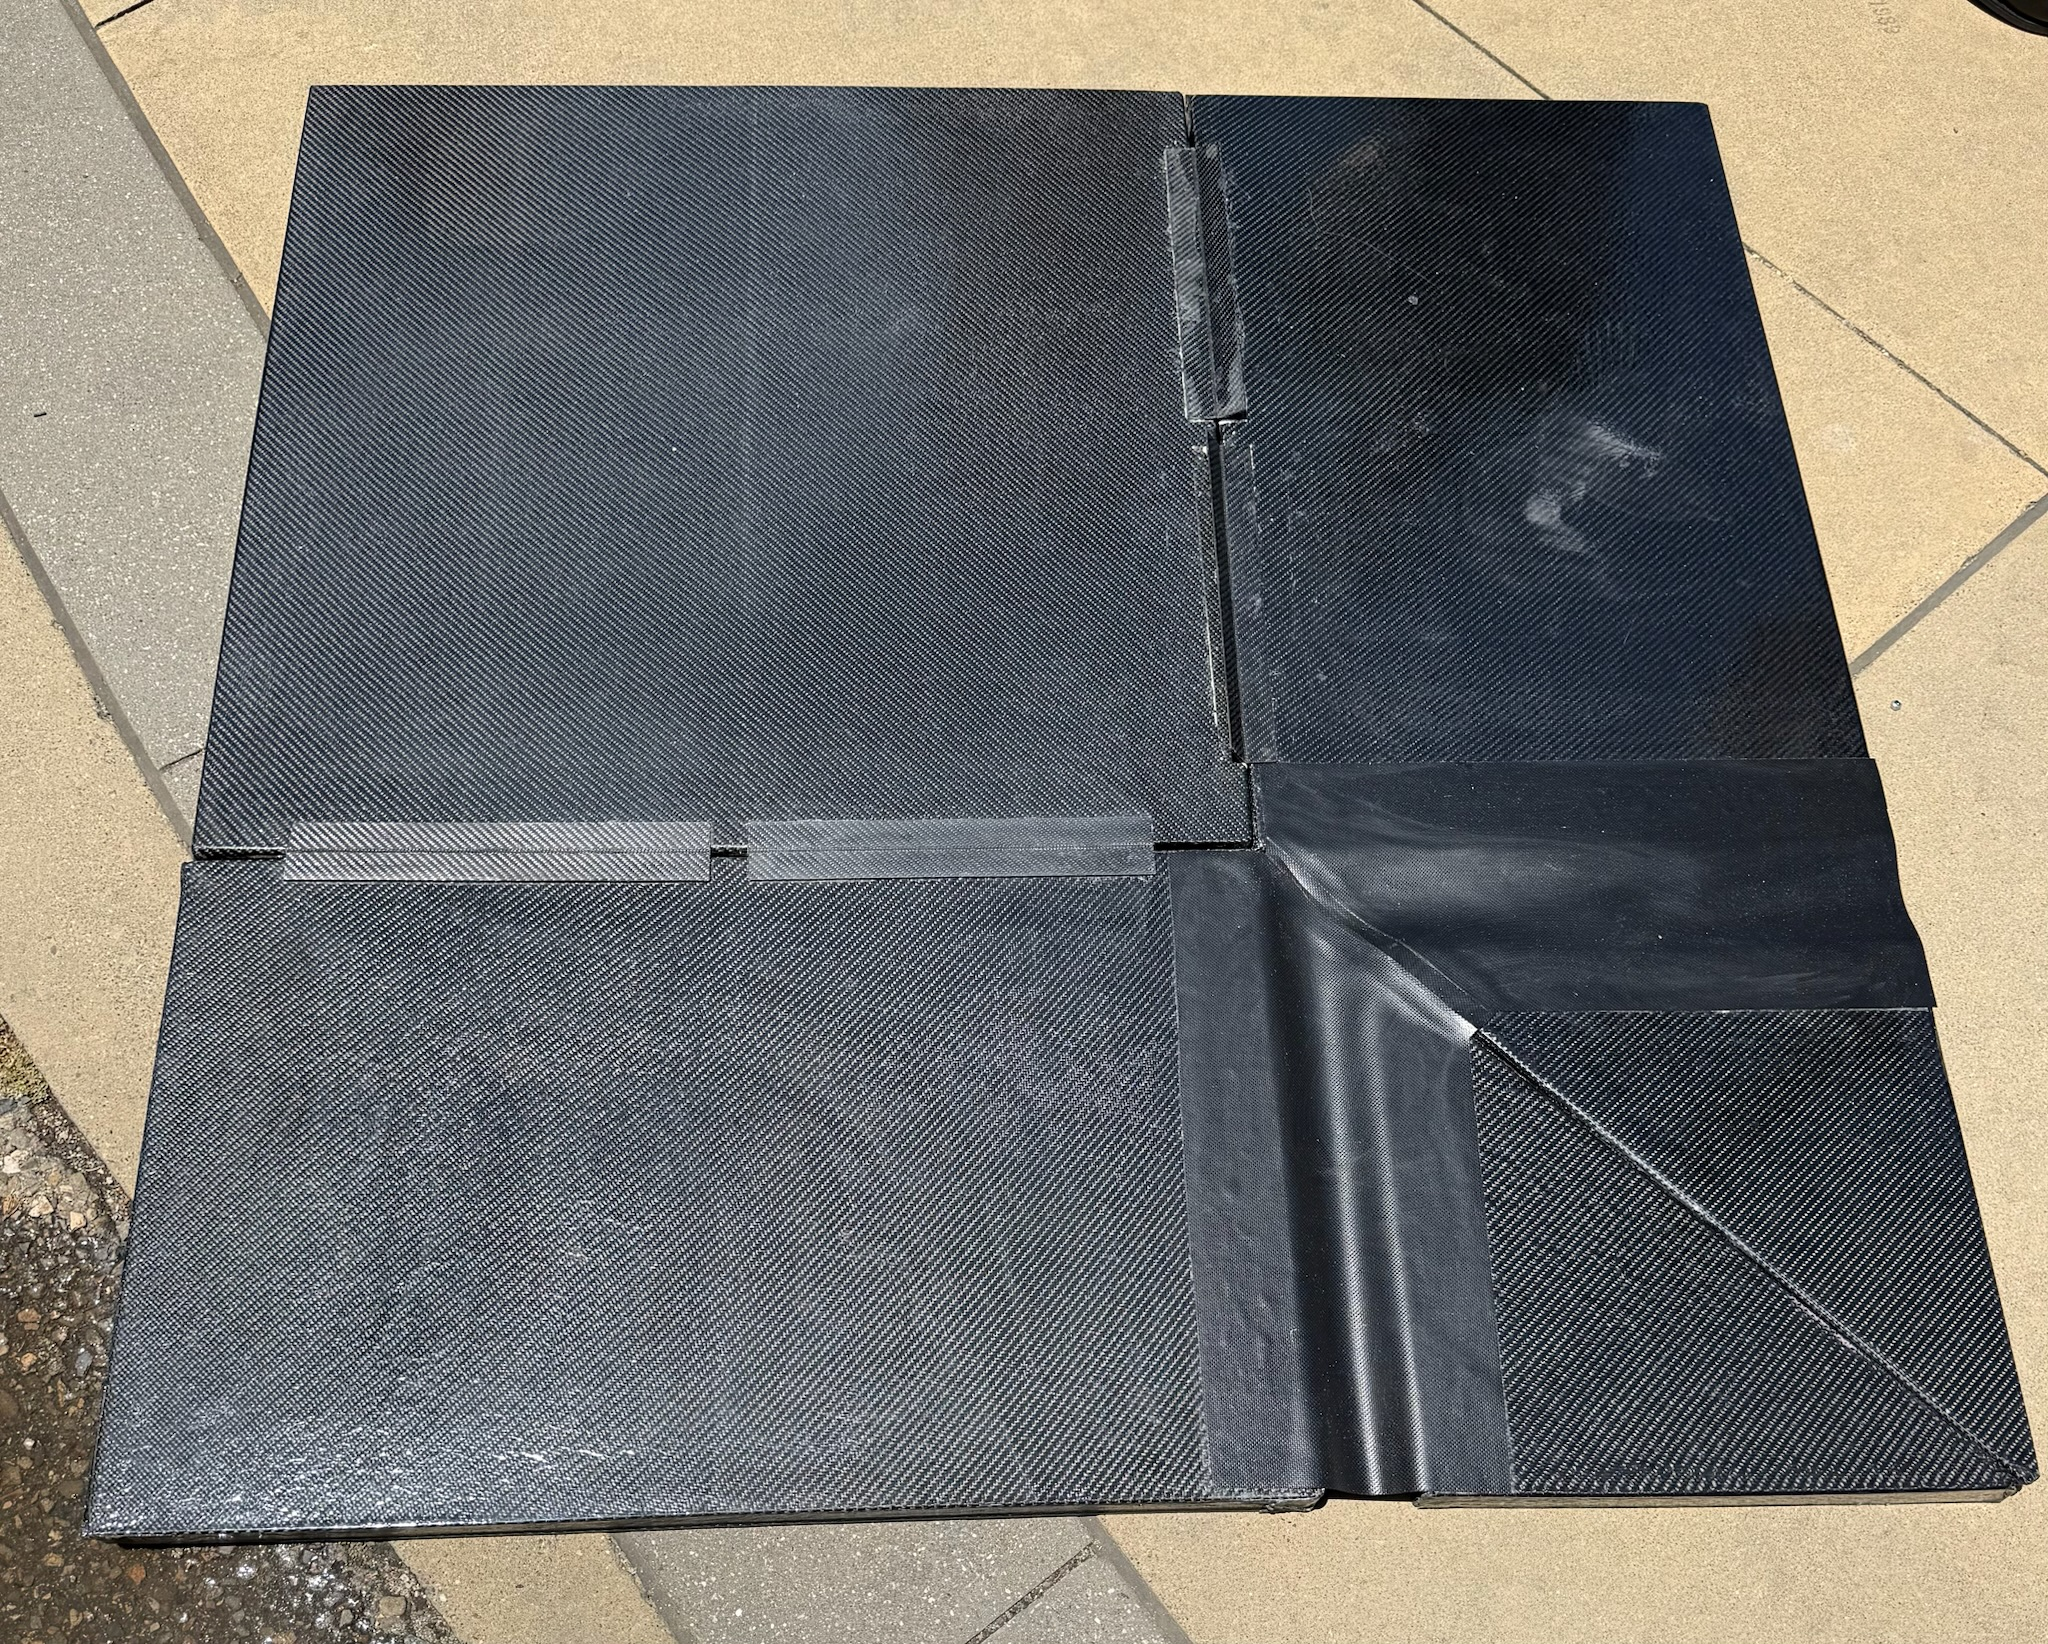
\includegraphics[
        width=2.35in,
        height=1.40in,
        keepaspectratio
    ]{refined_final_toro_cover_partial_carbon_model}
};
\draw[RuleGray,line width=0.55pt,rounded corners=4pt]
    ($(current page.north west)+(8.44in,-1.91in)$)
    rectangle
    ($(current page.north east)+(-0.42in,-3.40in)$);

% Captions
\node[anchor=north,text=Muted,font=\sffamily\fontsize{6.7}{7.3}\selectfont]
at ($(current page.north west)+(1.705in,-3.45in)$)
{Topcoat material preparation};

\node[anchor=north,text=Muted,font=\sffamily\fontsize{6.7}{7.3}\selectfont]
at ($(current page.north west)+(4.375in,-3.45in)$)
{Automotive-booth topcoat application};

\node[anchor=north,text=Muted,font=\sffamily\fontsize{6.7}{7.3}\selectfont]
at ($(current page.north west)+(7.045in,-3.45in)$)
{Coated panels drying after application};

\node[anchor=north,text=Muted,font=\sffamily\fontsize{6.7}{7.3}\selectfont]
at ($(current page.north west)+(9.50in,-3.45in)$)
{Partial carbon manufacturing model};

% Environmental rationale
\fill[SoftGold,rounded corners=4pt]
    ($(current page.north west)+(0.43in,-3.73in)$)
    rectangle
    ($(current page.north east)+(-0.42in,-4.76in)$);

\node[
    anchor=north west,
    align=left,
    text width=9.75in,
    text=Ink,
    font=\fontsize{7.05}{8.25}\selectfont
]
at ($(current page.north west)+(0.65in,-3.89in)$)
{
Because the sponsor required a carbon-fiber cover for outdoor use near chlorinated water,
environmental protection became a functional requirement rather than a cosmetic finish.
I selected and personally sprayed a UV-resistant Sunshield topcoat to seal minor laminate
porosity, reduce moisture ingress, preserve the carbon appearance, limit UV degradation of
the epoxy matrix, and isolate the composite surface from nearby metallic hardware.
};

% Results title
\node[
    anchor=north west,
    text=DeepGreen,
    font=\sffamily\bfseries\fontsize{8.0}{8.7}\selectfont
]
at ($(current page.north west)+(0.43in,-4.94in)$)
{FUNCTIONAL PROTOTYPE RESULTS};

% ------------------------------------------------------------
% Matched lower panels — larger type and improved allocation
% ------------------------------------------------------------

% Left results panel
\fill[SoftGreen,rounded corners=5pt]
    ($(current page.north west)+(0.43in,-5.22in)$)
    rectangle
    ($(current page.north west)+(5.98in,-7.39in)$);

\draw[RuleGray,line width=0.65pt,rounded corners=5pt]
    ($(current page.north west)+(0.43in,-5.22in)$)
    rectangle
    ($(current page.north west)+(5.98in,-7.39in)$);

\fill[DeepGreen,rounded corners=5pt]
    ($(current page.north west)+(0.43in,-5.22in)$)
    rectangle
    ($(current page.north west)+(5.98in,-5.58in)$);

\fill[DeepGreen]
    ($(current page.north west)+(0.43in,-5.40in)$)
    rectangle
    ($(current page.north west)+(5.98in,-5.58in)$);

\node[anchor=west,text=white,
      font=\sffamily\bfseries\fontsize{7.0}{7.6}\selectfont]
at ($(current page.north west)+(0.66in,-5.40in)$)
{SPECIFICATION};

\node[anchor=west,text=white,
      font=\sffamily\bfseries\fontsize{7.0}{7.6}\selectfont]
at ($(current page.north west)+(3.02in,-5.40in)$)
{RESULT};

\node[anchor=east,text=white,
      font=\sffamily\bfseries\fontsize{7.0}{7.6}\selectfont]
at ($(current page.north west)+(5.55in,-5.40in)$)
{STATUS};

\node[
    anchor=north west,
    align=left,
    text width=2.15in,
    text=Ink,
    font=\bfseries\fontsize{7.15}{8.55}\selectfont
]
at ($(current page.north west)+(0.66in,-5.72in)$)
{
Deployment time\\[3.4pt]
Removal time\\[3.4pt]
Single-user operation\\[3.4pt]
Single-side operation\\[3.4pt]
Deployment steps\\[3.4pt]
Removal steps\\[3.4pt]
Weight\\[3.4pt]
Folded storage
};

\node[
    anchor=north west,
    align=left,
    text width=1.45in,
    text=Ink,
    font=\fontsize{7.15}{8.55}\selectfont
]
at ($(current page.north west)+(3.02in,-5.72in)$)
{
25.51 seconds\\[3.4pt]
37.22 seconds\\[3.4pt]
100\% successful\\[3.4pt]
75\% successful\\[3.4pt]
6.4 average\\[3.4pt]
9 average\\[3.4pt]
17 lb\\[3.4pt]
2.9' x 2.9' x 1.7'
};

\node[
    anchor=north east,
    align=right,
    text width=1.05in,
    text=DeepGreen,
    font=\sffamily\bfseries\fontsize{7.05}{8.55}\selectfont
]
at ($(current page.north west)+(5.55in,-5.72in)$)
{
PASS\\[3.4pt]
PASS\\[3.4pt]
PASS\\[3.4pt]
NEAR TARGET\\[3.4pt]
PASS\\[3.4pt]
PASS\\[3.4pt]
NEAR TARGET\\[3.4pt]
PASS
};

% Right takeaways panel — widened for easier reading
\fill[SoftGreen,rounded corners=5pt]
    ($(current page.north west)+(6.14in,-5.22in)$)
    rectangle
    ($(current page.north east)+(-0.42in,-7.39in)$);

\draw[RuleGray,line width=0.65pt,rounded corners=5pt]
    ($(current page.north west)+(6.14in,-5.22in)$)
    rectangle
    ($(current page.north east)+(-0.42in,-7.39in)$);

\fill[DeepGreen,rounded corners=5pt]
    ($(current page.north west)+(6.14in,-5.22in)$)
    rectangle
    ($(current page.north east)+(-0.42in,-5.58in)$);

\fill[DeepGreen]
    ($(current page.north west)+(6.14in,-5.40in)$)
    rectangle
    ($(current page.north east)+(-0.42in,-5.58in)$);

\node[anchor=west,text=white,
      font=\sffamily\bfseries\fontsize{7.1}{7.7}\selectfont]
at ($(current page.north west)+(6.38in,-5.40in)$)
{ENGINEERING TAKEAWAYS};

\node[
    anchor=north west,
    align=left,
    text width=4.02in,
    text=Ink,
    font=\fontsize{6.75}{7.85}\selectfont
]
at ($(current page.north west)+(6.38in,-5.72in)$)
{
\textbf{Manufacturing first.}
Composite manufacturing constraints should guide the product architecture from the beginning.\\[4.5pt]
\textbf{Prioritize deliberately.}
Competing requirements must be balanced intentionally instead of maximizing every objective.\\[4.5pt]
\textbf{Lead through the process.}
Clear procedures, calm communication, and respect for teammates' strengths were essential during fabrication.\\[4.5pt]
\textbf{Next iteration.}
Reduce weight, refine the fabric-hinge fold lines, and improve panel-edge clearance.
};

% Compact concluding pathway
\node[
    anchor=center,
    align=center,
    text=PolyGold,
    font=\sffamily\bfseries\fontsize{6.3}{6.9}\selectfont
]
at ($(current page.north)+(3.06in,-7.18in)$)
{PROTOTYPE \faArrowRight\ DESIGN REFINEMENT
\faArrowRight\ REPEATABLE MANUFACTURING
\faArrowRight\ PRODUCT};

% Validation resources
\node[
    anchor=north,
    align=center,
    text=DeepGreen,
    font=\sffamily\bfseries\fontsize{6.6}{7.2}\selectfont
]
at ($(current page.north)+(0,-7.58in)$)
{\href{\ToroDeploymentLink}{\faPlayCircle\ DEPLOYMENT}
\hspace{18pt}
\href{\ToroRemovalLink}{\faPlayCircle\ REMOVAL / FOLDING}
\hspace{18pt}
\href{\ToroPosterLink}{\faFilePdf\ EXPO POSTER}
\hspace{18pt}
\href{\ToroReportLink}{\faFilePdf\ FINAL REPORT}};

% Footer
\node[
    anchor=south west,
    text=white,
    font=\sffamily\bfseries\fontsize{7.1}{7.7}\selectfont
]
at ($(current page.south west)+(0.42in,0.17in)$)
{\faArrowLeft\ MANUFACTURING-DRIVEN DESIGN};

\node[
    anchor=south,
    text=white,
    font=\sffamily\fontsize{7.0}{7.6}\selectfont
]
at ($(current page.south)+(0,0.17in)$)
{TORO COVER \hspace{6pt} 3 / 3};

\node[
    anchor=south east,
    text=white,
    font=\sffamily\bfseries\fontsize{7.1}{7.7}\selectfont
]
at ($(current page.south east)+(-0.42in,0.17in)$)
{NEXT PROJECT \faArrowRight};

\end{tikzpicture}
\input{paddle}
\clearpage
.
% 2. In main.tex, place 
% ============================================================
% TORO COVER — THREE-PAGE PORTFOLIO CASE STUDY
% Pages 3–5 of the complete portfolio
%
% IMPORTANT:
% 1. This file must NOT contain \documentclass, \begin{document},
%    \end{document}, or \input{toro}.
% 2. In main.tex, place \input{toro} before \end{document}.
% 3. Image references use the original Overleaf base filenames
%    without extensions.
% ============================================================



% ============================================================
% CLICKABLE PROJECT RESOURCES
% All links use the exact Google Drive resources supplied.
% ============================================================
\providecommand{\ToroDrawingLink}{https://drive.google.com/file/d/1A7-7wMnRNLuQDaTgxeuUCBsGNqyXzOGV/view?usp=sharing}
\providecommand{\ToroDimensionsLink}{https://drive.google.com/file/d/13sw3BNJvE8GdzlRffxoF2n5r9Gzxide7/view?usp=sharing}
\providecommand{\ToroProblemLink}{https://drive.google.com/file/d/1zHtl8zrb13F1yeN74ptawpfS5UM_xsuw/view?usp=drive_link}
\providecommand{\ToroReportLink}{https://drive.google.com/file/d/1ULZ-P46lFsC2x29ZfmRVIKgYnr9o8hMt/view?usp=drive_link}
\providecommand{\ToroPosterLink}{https://drive.google.com/file/d/1vKiKaJUcHQb_db-FkZnRF6EvtuM4hKyS/view?usp=drive_link}
\providecommand{\ToroDeploymentLink}{https://drive.google.com/file/d/1XJx34o80_mZPTl7xy93HtWAgtS3ThhvY/view?usp=drive_link}
\providecommand{\ToroRemovalLink}{https://drive.google.com/file/d/1O7xYeyB67NUwT-j1B1HeiCcHnZDYjk6_/view?usp=drive_link}

% ============================================================
% PAGE 1 — PROJECT OVERVIEW, OWNERSHIP, AND ARCHITECTURE
% ============================================================

\clearpage
\thispagestyle{empty}
\hypertarget{toro}{}
\null

\begin{tikzpicture}[remember picture,overlay]

% Background
\fill[white]
    (current page.south west)
    rectangle
    (current page.north east);

% Page bars
\fill[DeepGreen]
    (current page.north west)
    rectangle
    ($(current page.north east)+(0,-0.095in)$);

\fill[PolyGold]
    ($(current page.north west)+(0,-0.095in)$)
    rectangle
    ($(current page.north east)+(0,-0.14in)$);

\fill[DeepGreen]
    (current page.south west)
    rectangle
    ($(current page.south east)+(0,0.36in)$);

\fill[PolyGold]
    ($(current page.south west)+(0,0.36in)$)
    rectangle
    ($(current page.south east)+(0,0.405in)$);

% Header
\node[
    anchor=north west,
    text=PolyGold,
    font=\sffamily\bfseries\fontsize{8.1}{8.7}\selectfont
]
at ($(current page.north west)+(0.42in,-0.39in)$)
{01 COMPOSITES \hspace{5pt}/\hspace{5pt} PROJECT 01};

\node[
    anchor=north west,
    text=DeepGreen,
    font=\bfseries\fontsize{23.5}{24.5}\selectfont
]
at ($(current page.north west)+(0.40in,-0.67in)$)
{TORO CARBON FIBER SAFETY COVER};

\node[
    anchor=north west,
    text=Muted,
    font=\sffamily\fontsize{8.4}{9.2}\selectfont
]
at ($(current page.north west)+(0.42in,-1.12in)$)
{Cal Poly Composites Laboratory \hspace{7pt}\textbullet\hspace{7pt}
Team Project \hspace{7pt}\textbullet\hspace{7pt}
Fall--Spring 2026 \hspace{7pt}\textbullet\hspace{7pt}
San Luis Obispo, California};

\fill[PolyGold]
    ($(current page.north west)+(0.42in,-1.37in)$)
    rectangle
    ($(current page.north west)+(6.1in,-1.325in)$);

% Challenge text
\node[
    anchor=north west,
    text=DeepGreen,
    font=\sffamily\bfseries\fontsize{8.1}{8.8}\selectfont
]
at ($(current page.north west)+(0.43in,-1.61in)$)
{THE CHALLENGE};

\node[
    anchor=north west,
    align=left,
    text width=4.47in,
    text=Ink,
    font=\fontsize{8.05}{9.65}\selectfont
]
at ($(current page.north west)+(0.43in,-1.84in)$)
{
Develop a lightweight cover for a 6 ft by 6 ft in-ground spa
that could be deployed by one person, stored compactly,
provide insulation, resist a poolside environment, and maintain
a refined appearance. The sponsor supplied an ambitious but
intentionally broad project statement, requiring the team to
define the product architecture, priorities, manufacturing
strategy, and realistic path toward future commercialization.
};

% Role box
\fill[SoftGold,rounded corners=5pt]
    ($(current page.north west)+(0.42in,-2.88in)$)
    rectangle
    ($(current page.north west)+(4.98in,-4.58in)$);

\fill[PolyGold]
    ($(current page.north west)+(0.42in,-2.88in)$)
    rectangle
    ($(current page.north west)+(0.52in,-4.58in)$);

\node[
    anchor=north west,
    text=DeepGreen,
    font=\sffamily\bfseries\fontsize{8.1}{8.8}\selectfont
]
at ($(current page.north west)+(0.66in,-3.02in)$)
{MY ROLE — DESIGN \& MANUFACTURING LEAD};

\node[
    anchor=north west,
    align=left,
    text width=4.02in,
    text=Ink,
    font=\fontsize{7.05}{8.15}\selectfont
]
at ($(current page.north west)+(0.66in,-3.27in)$)
{
\textbullet\ Modeled every custom part and the complete assembly\\[1.5pt]
\textbullet\ Produced the engineering drawing package independently\\[1.5pt]
\textbullet\ Developed the composite-panel manufacturing process\\[1.5pt]
\textbullet\ Created all waterjet DXFs and manufacturing geometry\\[1.5pt]
\textbullet\ Trained teammates in wet layup and vacuum bagging\\[1.5pt]
\textbullet\ Presented feasibility, scope, and tradeoffs to the sponsor
};

% Large deployed foam-model image
\node[anchor=center,inner sep=0pt]
at ($(current page.north west)+(8.00in,-3.04in)$)
{
    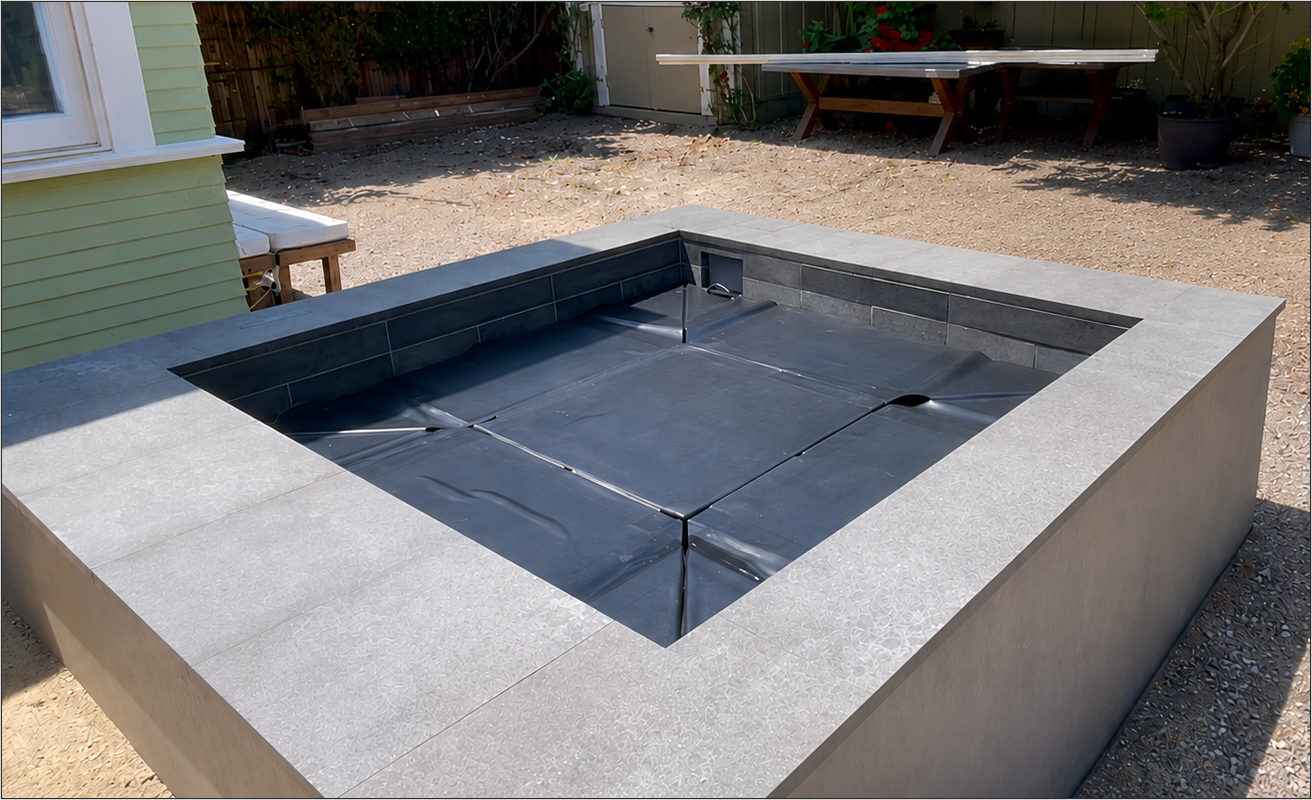
\includegraphics[
        width=5.55in,
        height=2.78in,
        keepaspectratio
    ]{deployed_functional_prototype}
};

\draw[DeepGreen,line width=0.8pt,rounded corners=7pt]
    ($(current page.north west)+(5.16in,-1.61in)$)
    rectangle
    ($(current page.north east)+(-0.42in,-4.47in)$);

\node[
    anchor=north west,
    text=Muted,
    font=\sffamily\fontsize{6.2}{6.9}\selectfont
]
at ($(current page.north west)+(5.18in,-4.54in)$)
{Functional foam model deployed over the sponsor's in-ground spa.};

% Image-strip title
\node[
    anchor=north west,
    text=DeepGreen,
    font=\sffamily\bfseries\fontsize{8.1}{8.8}\selectfont
]
at ($(current page.north west)+(0.43in,-4.78in)$)
{PRODUCT DEVELOPMENT AND FINAL ARCHITECTURE};

% Five-image development strip — CAD-first sequence
% Image 1: topside CAD
\node[anchor=center,inner sep=0pt]
at ($(current page.north west)+(1.47in,-5.73in)$)
{
    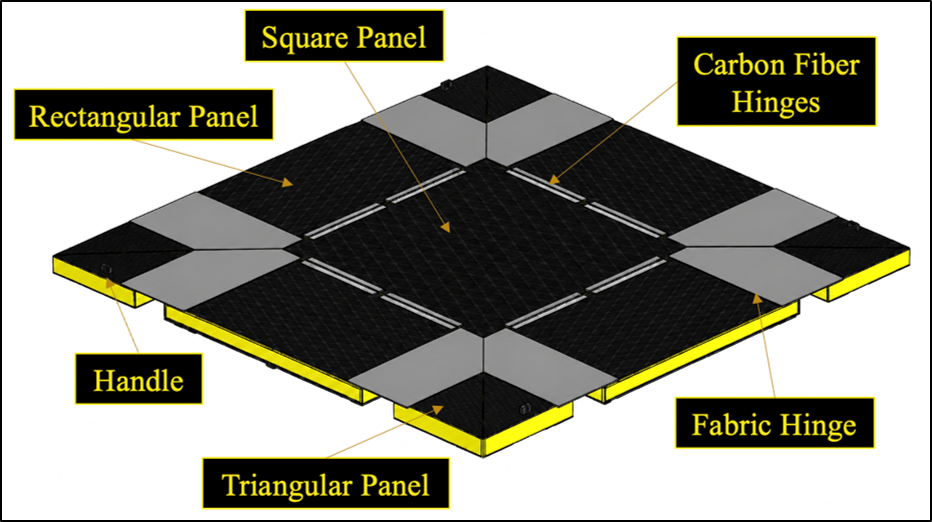
\includegraphics[
        width=1.92in,
        height=1.30in,
        keepaspectratio
    ]{Toro_Cover_topside_Cad}
};
\draw[RuleGray,line width=0.55pt,rounded corners=4pt]
    ($(current page.north west)+(0.43in,-5.04in)$)
    rectangle
    ($(current page.north west)+(2.51in,-6.43in)$);

% Image 2: underside CAD
\node[anchor=center,inner sep=0pt]
at ($(current page.north west)+(3.66in,-5.73in)$)
{
    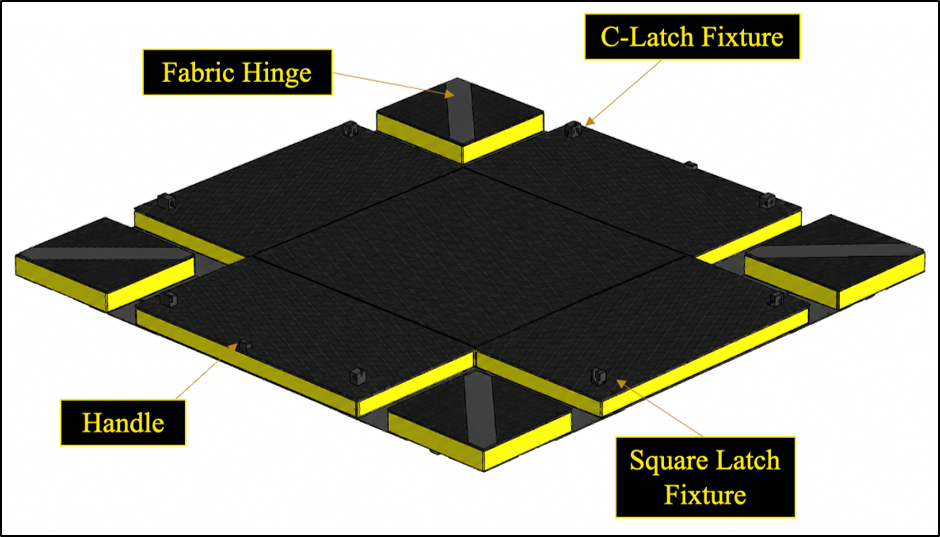
\includegraphics[
        width=1.92in,
        height=1.30in,
        keepaspectratio
    ]{toro_cover_underside_cad}
};
\draw[RuleGray,line width=0.55pt,rounded corners=4pt]
    ($(current page.north west)+(2.62in,-5.04in)$)
    rectangle
    ($(current page.north west)+(4.70in,-6.43in)$);

% Image 3: folded CAD
\node[anchor=center,inner sep=0pt]
at ($(current page.north west)+(5.85in,-5.73in)$)
{
    \includegraphics[
        width=1.92in,
        height=1.30in,
        keepaspectratio
    ]{\detokenize{Toro_Cover_folded Configuration}}
};
\draw[RuleGray,line width=0.55pt,rounded corners=4pt]
    ($(current page.north west)+(4.81in,-5.04in)$)
    rectangle
    ($(current page.north west)+(6.89in,-6.43in)$);

% Image 4: dual-use product concept
\node[anchor=center,inner sep=0pt]
at ($(current page.north west)+(8.04in,-5.73in)$)
{
    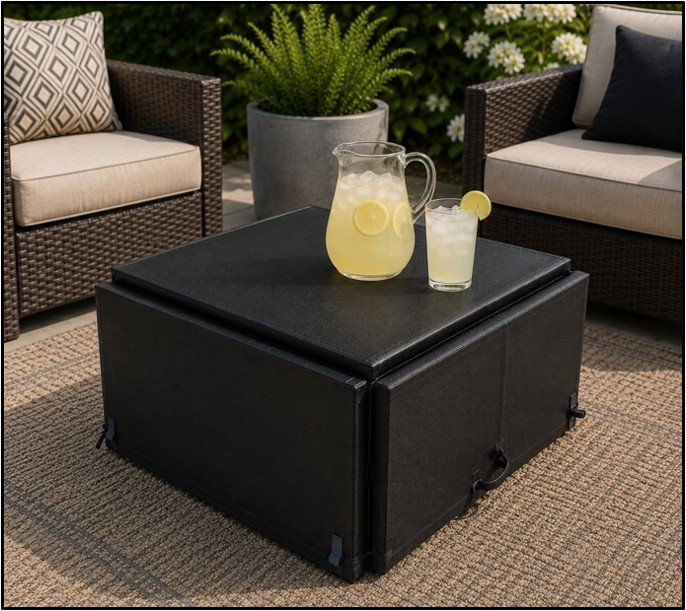
\includegraphics[
        width=1.92in,
        height=1.30in,
        keepaspectratio
    ]{generative_AI_concept_toro_cover_art}
};
\draw[RuleGray,line width=0.55pt,rounded corners=4pt]
    ($(current page.north west)+(7.00in,-5.04in)$)
    rectangle
    ($(current page.north west)+(9.08in,-6.43in)$);

% Image 5: folded foam functional prototype
% The portrait photograph is deliberately clipped to the landscape frame
% so the ottoman fills the card without extending beyond its border.
\begin{scope}
\clip[rounded corners=4pt]
    ($(current page.north west)+(9.19in,-5.04in)$)
    rectangle
    ($(current page.north east)+(-0.43in,-6.43in)$);

% Keep the original image proportions and center it within the existing card.
\node[anchor=center,inner sep=0pt]
at ($(current page.north west)+(9.88in,-5.735in)$)
{
    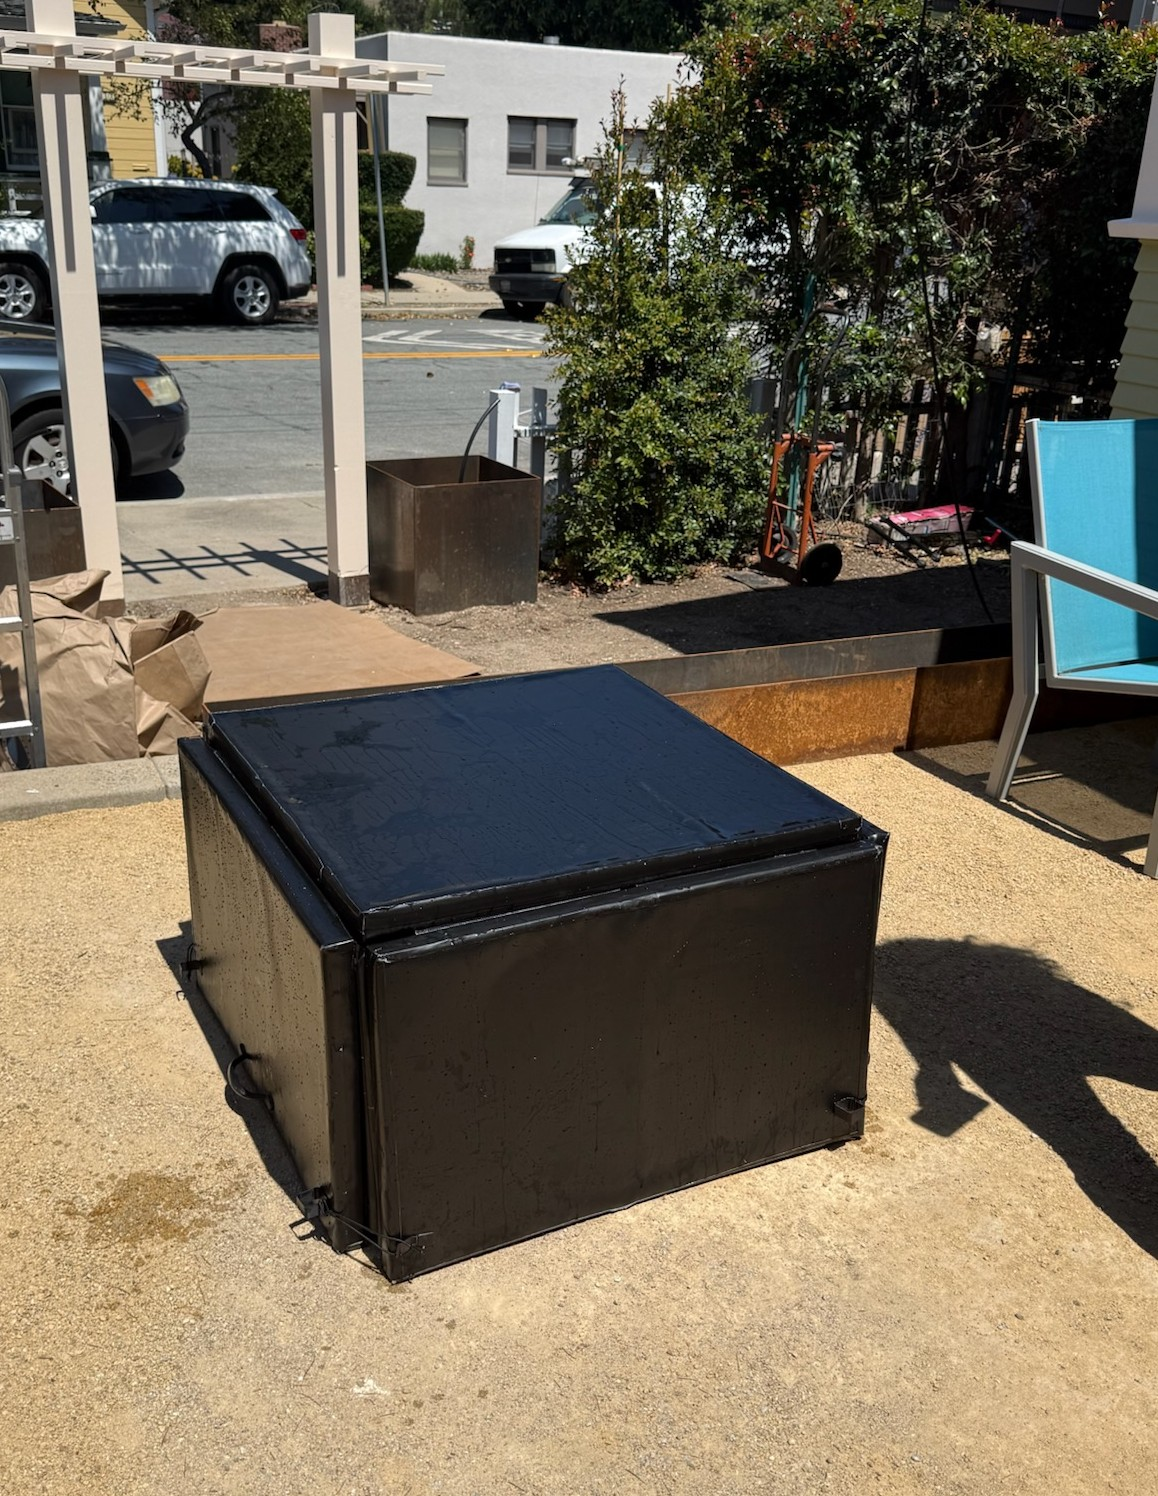
\includegraphics[
        width=1.58in,
        height=1.28in,
        keepaspectratio
    ]{foam_model_folded_backyard_image}
};
\end{scope}

\draw[RuleGray,line width=0.55pt,rounded corners=4pt]
    ($(current page.north west)+(9.19in,-5.04in)$)
    rectangle
    ($(current page.north east)+(-0.43in,-6.43in)$);

% Larger captions
\node[anchor=north,align=center,text width=1.95in,text=Muted,
      font=\sffamily\fontsize{6.8}{7.4}\selectfont]
at ($(current page.north west)+(1.47in,-6.49in)$)
{Topside panel architecture};

\node[anchor=north,align=center,text width=1.95in,text=Muted,
      font=\sffamily\fontsize{6.8}{7.4}\selectfont]
at ($(current page.north west)+(3.66in,-6.49in)$)
{Underside hinge architecture};

\node[anchor=north,align=center,text width=1.95in,text=Muted,
      font=\sffamily\fontsize{6.8}{7.4}\selectfont]
at ($(current page.north west)+(5.85in,-6.49in)$)
{Folded CAD configuration};

\node[anchor=north,align=center,text width=1.95in,text=Muted,
      font=\sffamily\fontsize{6.8}{7.4}\selectfont]
at ($(current page.north west)+(8.04in,-6.49in)$)
{Dual-use product vision};

\node[anchor=north,align=center,text width=1.95in,text=Muted,
      font=\sffamily\fontsize{6.8}{7.4}\selectfont]
at ($(current page.north west)+(9.88in,-6.49in)$)
{Folded foam prototype};

% Page 1 resource bar — centered and non-repeated resources
\fill[Panel,rounded corners=4pt]
    ($(current page.north west)+(0.43in,-7.05in)$)
    rectangle
    ($(current page.north east)+(-0.43in,-7.64in)$);
\draw[RuleGray,line width=0.5pt,rounded corners=4pt]
    ($(current page.north west)+(0.43in,-7.05in)$)
    rectangle
    ($(current page.north east)+(-0.43in,-7.64in)$);

\node[
    anchor=center,
    align=center,
    text=DeepGreen,
    font=\sffamily\bfseries\fontsize{6.9}{7.5}\selectfont
]
at ($(current page.north)+(0,-7.345in)$)
{\href{\ToroDrawingLink}{\faDraftingCompass\ DRAWING PACKAGE}
\hspace{24pt}
\href{\ToroDimensionsLink}{\faImage\ DIMENSION STUDY}
\hspace{24pt}
\href{\ToroProblemLink}{\faFileImage\ PROBLEM STATEMENT}};

% Footer
\node[
    anchor=south west,
    text=white,
    font=\sffamily\bfseries\fontsize{7.1}{7.7}\selectfont
]
at ($(current page.south west)+(0.42in,0.17in)$)
{\hyperlink{composites}{\faArrowLeft\ COMPOSITES}};

\node[
    anchor=south,
    text=white,
    font=\sffamily\fontsize{7.0}{7.6}\selectfont
]
at ($(current page.south)+(0,0.17in)$)
{TORO COVER \hspace{6pt} 1 / 3};

\node[
    anchor=south east,
    text=white,
    font=\sffamily\bfseries\fontsize{7.1}{7.7}\selectfont
]
at ($(current page.south east)+(-0.42in,0.17in)$)
{MANUFACTURING-DRIVEN DESIGN \faArrowRight};

\end{tikzpicture}


% ============================================================
% PAGE 2 — MANUFACTURING-DRIVEN DESIGN
% ============================================================

\clearpage
\thispagestyle{empty}
\hypertarget{toro-manufacturing}{}
\null

\begin{tikzpicture}[remember picture,overlay]

% Background and bars
\fill[white]
    (current page.south west)
    rectangle
    (current page.north east);

\fill[DeepGreen]
    (current page.north west)
    rectangle
    ($(current page.north east)+(0,-0.095in)$);

\fill[PolyGold]
    ($(current page.north west)+(0,-0.095in)$)
    rectangle
    ($(current page.north east)+(0,-0.14in)$);

\fill[DeepGreen]
    (current page.south west)
    rectangle
    ($(current page.south east)+(0,0.36in)$);

\fill[PolyGold]
    ($(current page.south west)+(0,0.36in)$)
    rectangle
    ($(current page.south east)+(0,0.405in)$);

% Header
\node[
    anchor=north west,
    text=PolyGold,
    font=\sffamily\bfseries\fontsize{8.1}{8.7}\selectfont
]
at ($(current page.north west)+(0.42in,-0.39in)$)
{TORO COVER \hspace{5pt}/\hspace{5pt} DESIGN FOR MANUFACTURABILITY};

\node[
    anchor=north west,
    text=DeepGreen,
    font=\bfseries\fontsize{23}{24}\selectfont
]
at ($(current page.north west)+(0.40in,-0.67in)$)
{THE ENVELOPE METHOD};

\node[
    anchor=north west,
    text=Muted,
    font=\sffamily\fontsize{8.7}{9.6}\selectfont
]
at ($(current page.north west)+(0.42in,-1.12in)$)
{A one-layup process developed for unusually thick insulated composite sandwich panels};

\fill[PolyGold]
    ($(current page.north west)+(0.42in,-1.36in)$)
    rectangle
    ($(current page.north west)+(5.30in,-1.315in)$);

% Process explanation
\fill[SoftGold,rounded corners=5pt]
    ($(current page.north west)+(0.42in,-1.61in)$)
    rectangle
    ($(current page.north east)+(-0.42in,-2.90in)$);

\fill[PolyGold]
    ($(current page.north west)+(0.42in,-1.61in)$)
    rectangle
    ($(current page.north west)+(0.52in,-2.90in)$);

\node[
    anchor=north west,
    text=DeepGreen,
    font=\sffamily\bfseries\fontsize{7.9}{8.6}\selectfont
]
at ($(current page.north west)+(0.67in,-1.76in)$)
{PROCESS INNOVATION};

\node[
    anchor=north west,
    align=left,
    text width=9.55in,
    text=Ink,
    font=\fontsize{7.35}{8.75}\selectfont
]
at ($(current page.north west)+(0.67in,-2.02in)$)
{
Weight reduction and insulation were both essential, leading to the selection of an
XPS foam core. Because XPS could not tolerate composite heat-cure temperatures, prepreg
processing was not practical and the panels had to be manufactured by wet layup with a
room-temperature cure. To simplify this process, I waterjet-cut XPS perimeter strips from
excess foam and placed them around each core inside the vacuum enclosure. Under vacuum,
the top and bottom carbon skins met along the panel sides and compressed against this
border, eliminating a separate edge-banding layup and reducing corner pleating.
};

% Workflow title
\node[
    anchor=north west,
    text=DeepGreen,
    font=\sffamily\bfseries\fontsize{8.0}{8.7}\selectfont
]
at ($(current page.north west)+(0.43in,-3.06in)$)
{MANUFACTURING WORKFLOW};

% Row 1 image 1
\node[anchor=center,inner sep=0pt]
at ($(current page.north west)+(2.07in,-4.105in)$)
{
    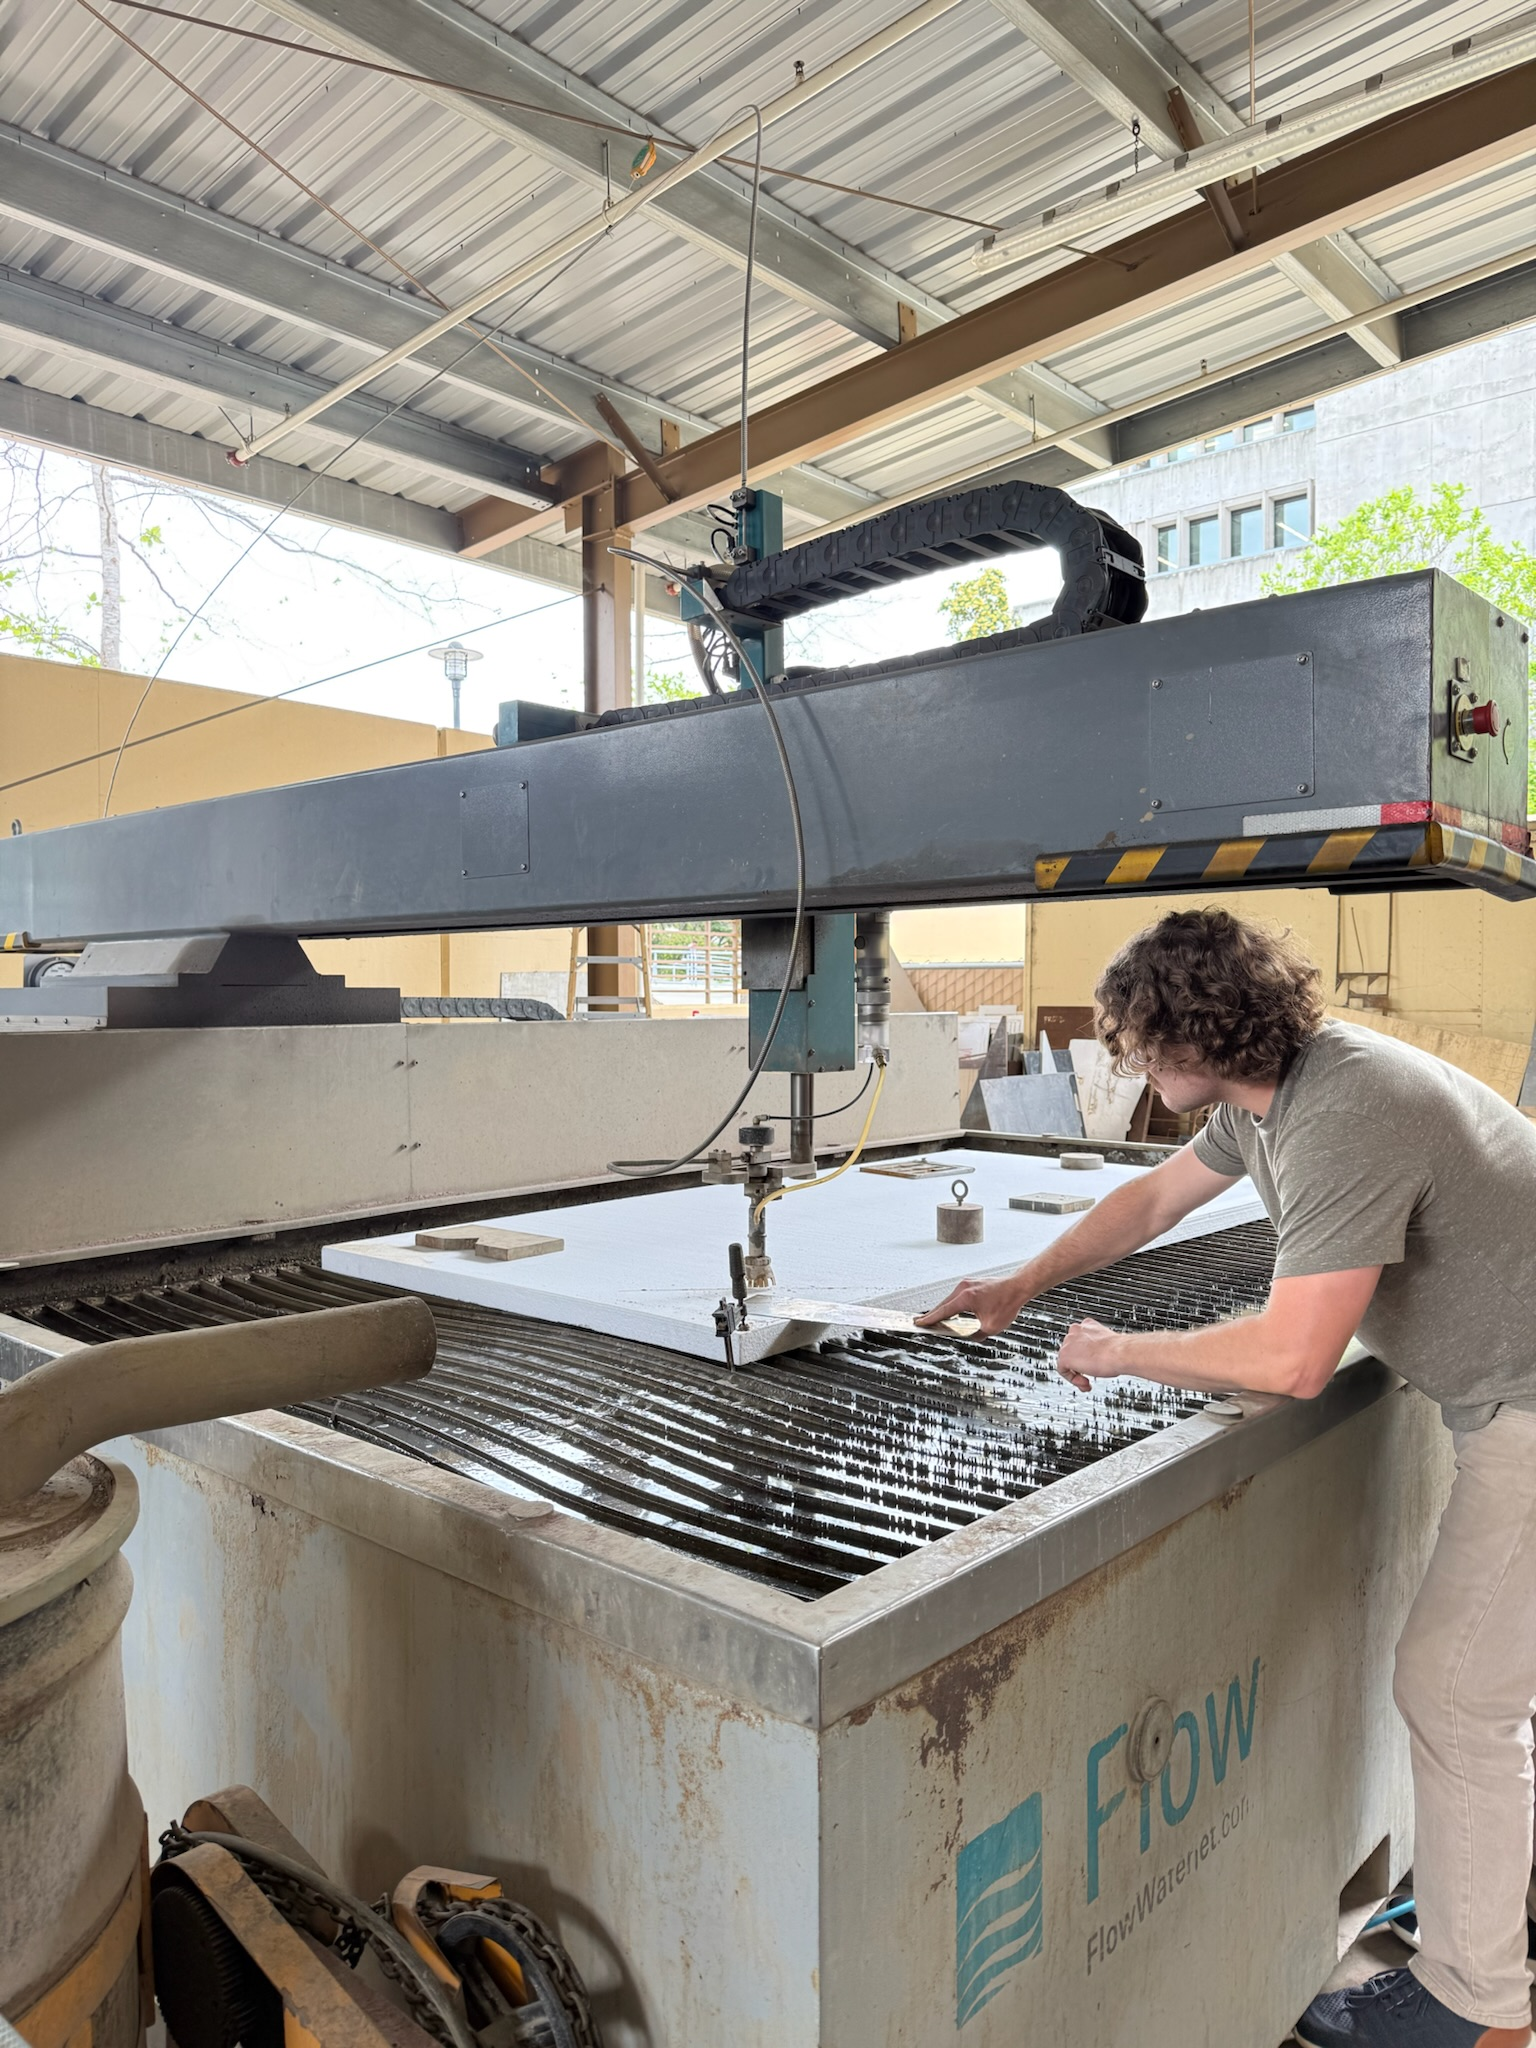
\includegraphics[
        width=3.10in,
        height=1.40in,
        keepaspectratio
    ]{waterjet_foam}
};
\draw[RuleGray,line width=0.55pt,rounded corners=4pt]
    ($(current page.north west)+(0.43in,-3.36in)$)
    rectangle
    ($(current page.north west)+(3.71in,-4.85in)$);

% Row 1 image 2
\node[anchor=center,inner sep=0pt]
at ($(current page.north west)+(5.50in,-4.105in)$)
{
    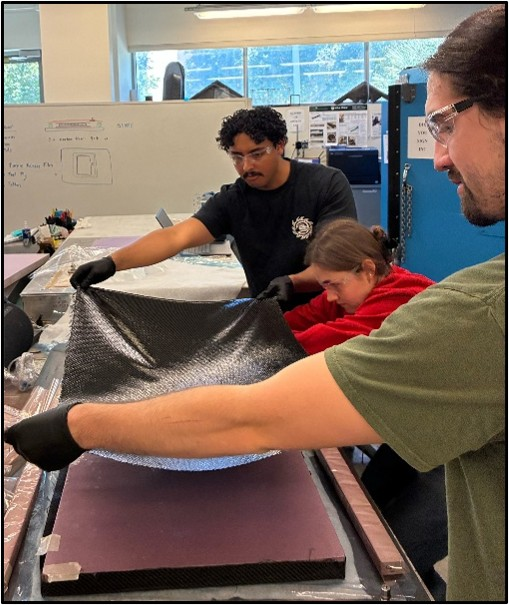
\includegraphics[
        width=3.10in,
        height=1.40in,
        keepaspectratio
    ]{group_layup}
};
\draw[RuleGray,line width=0.55pt,rounded corners=4pt]
    ($(current page.north west)+(3.86in,-3.36in)$)
    rectangle
    ($(current page.north west)+(7.14in,-4.85in)$);

% Row 1 image 3
\node[anchor=center,inner sep=0pt]
at ($(current page.north west)+(8.935in,-4.105in)$)
{
    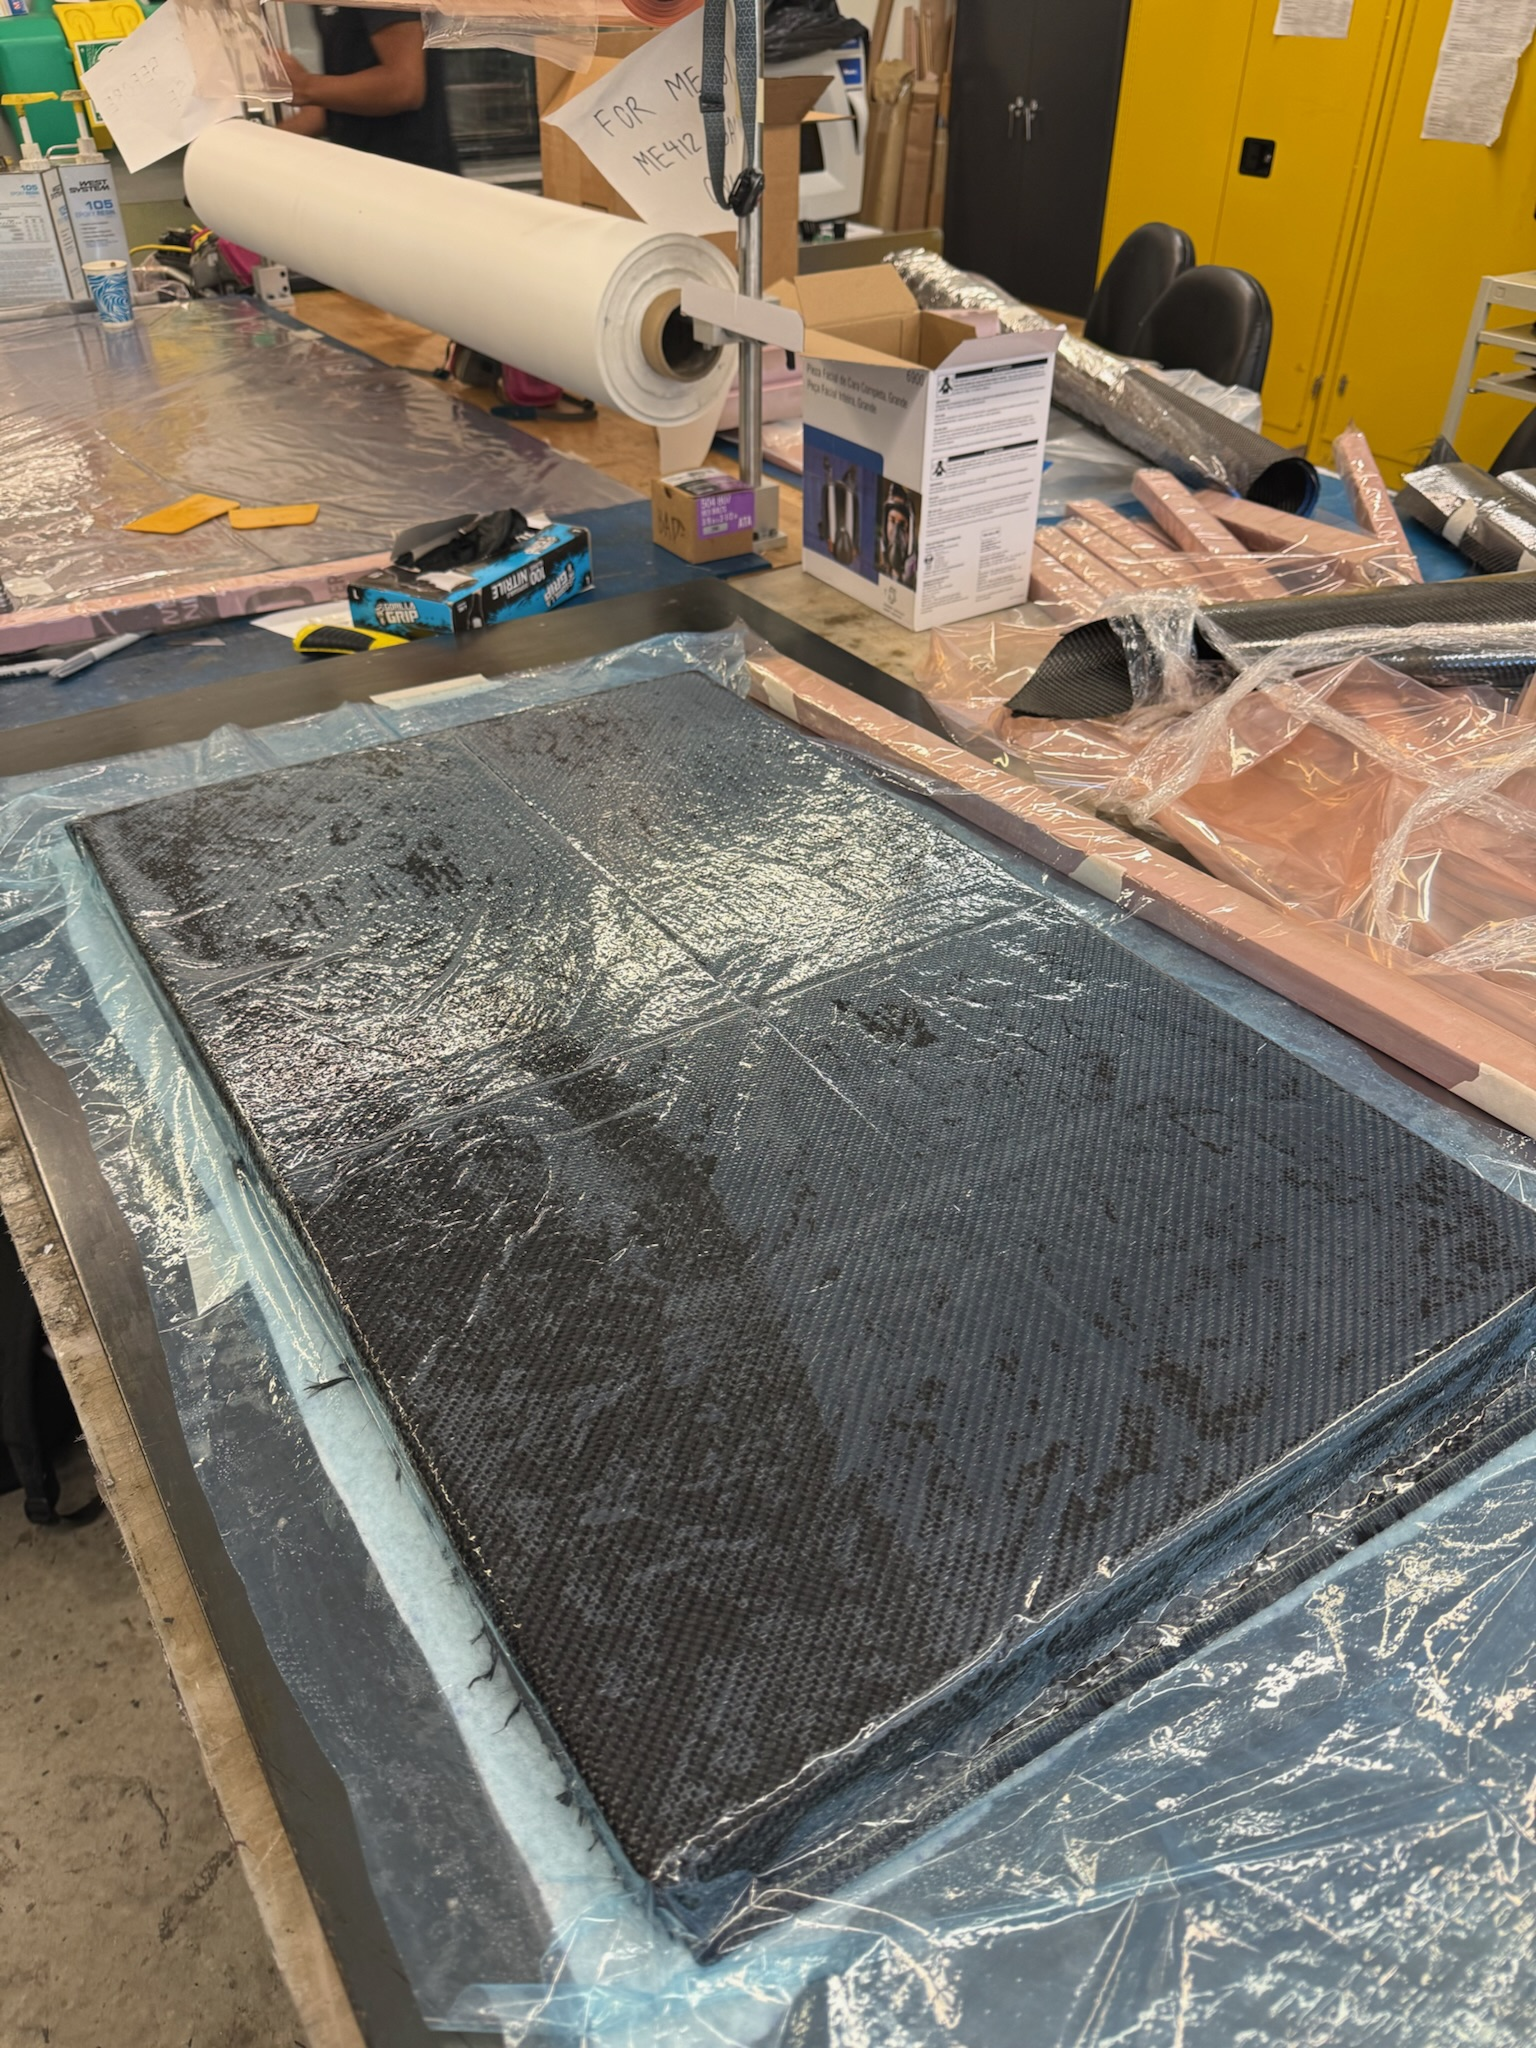
\includegraphics[
        width=3.10in,
        height=1.40in,
        keepaspectratio
    ]{blue_perforrated_film_layup}
};
\draw[RuleGray,line width=0.55pt,rounded corners=4pt]
    ($(current page.north west)+(7.29in,-3.36in)$)
    rectangle
    ($(current page.north east)+(-0.42in,-4.85in)$);

% Row 1 captions
\node[anchor=north,text=Muted,font=\sffamily\fontsize{6.7}{7.3}\selectfont]
at ($(current page.north west)+(2.07in,-4.90in)$)
{1. Waterjet-cut core and perimeter geometry};

\node[anchor=north,text=Muted,font=\sffamily\fontsize{6.7}{7.3}\selectfont]
at ($(current page.north west)+(5.50in,-4.90in)$)
{2. Team wet layup under my process guidance};

\node[anchor=north,text=Muted,font=\sffamily\fontsize{6.7}{7.3}\selectfont]
at ($(current page.north west)+(8.935in,-4.90in)$)
{3. Perforated film, breather, and vacuum enclosure};

% Row 2 image 1
\node[anchor=center,inner sep=0pt]
at ($(current page.north west)+(2.07in,-5.875in)$)
{
    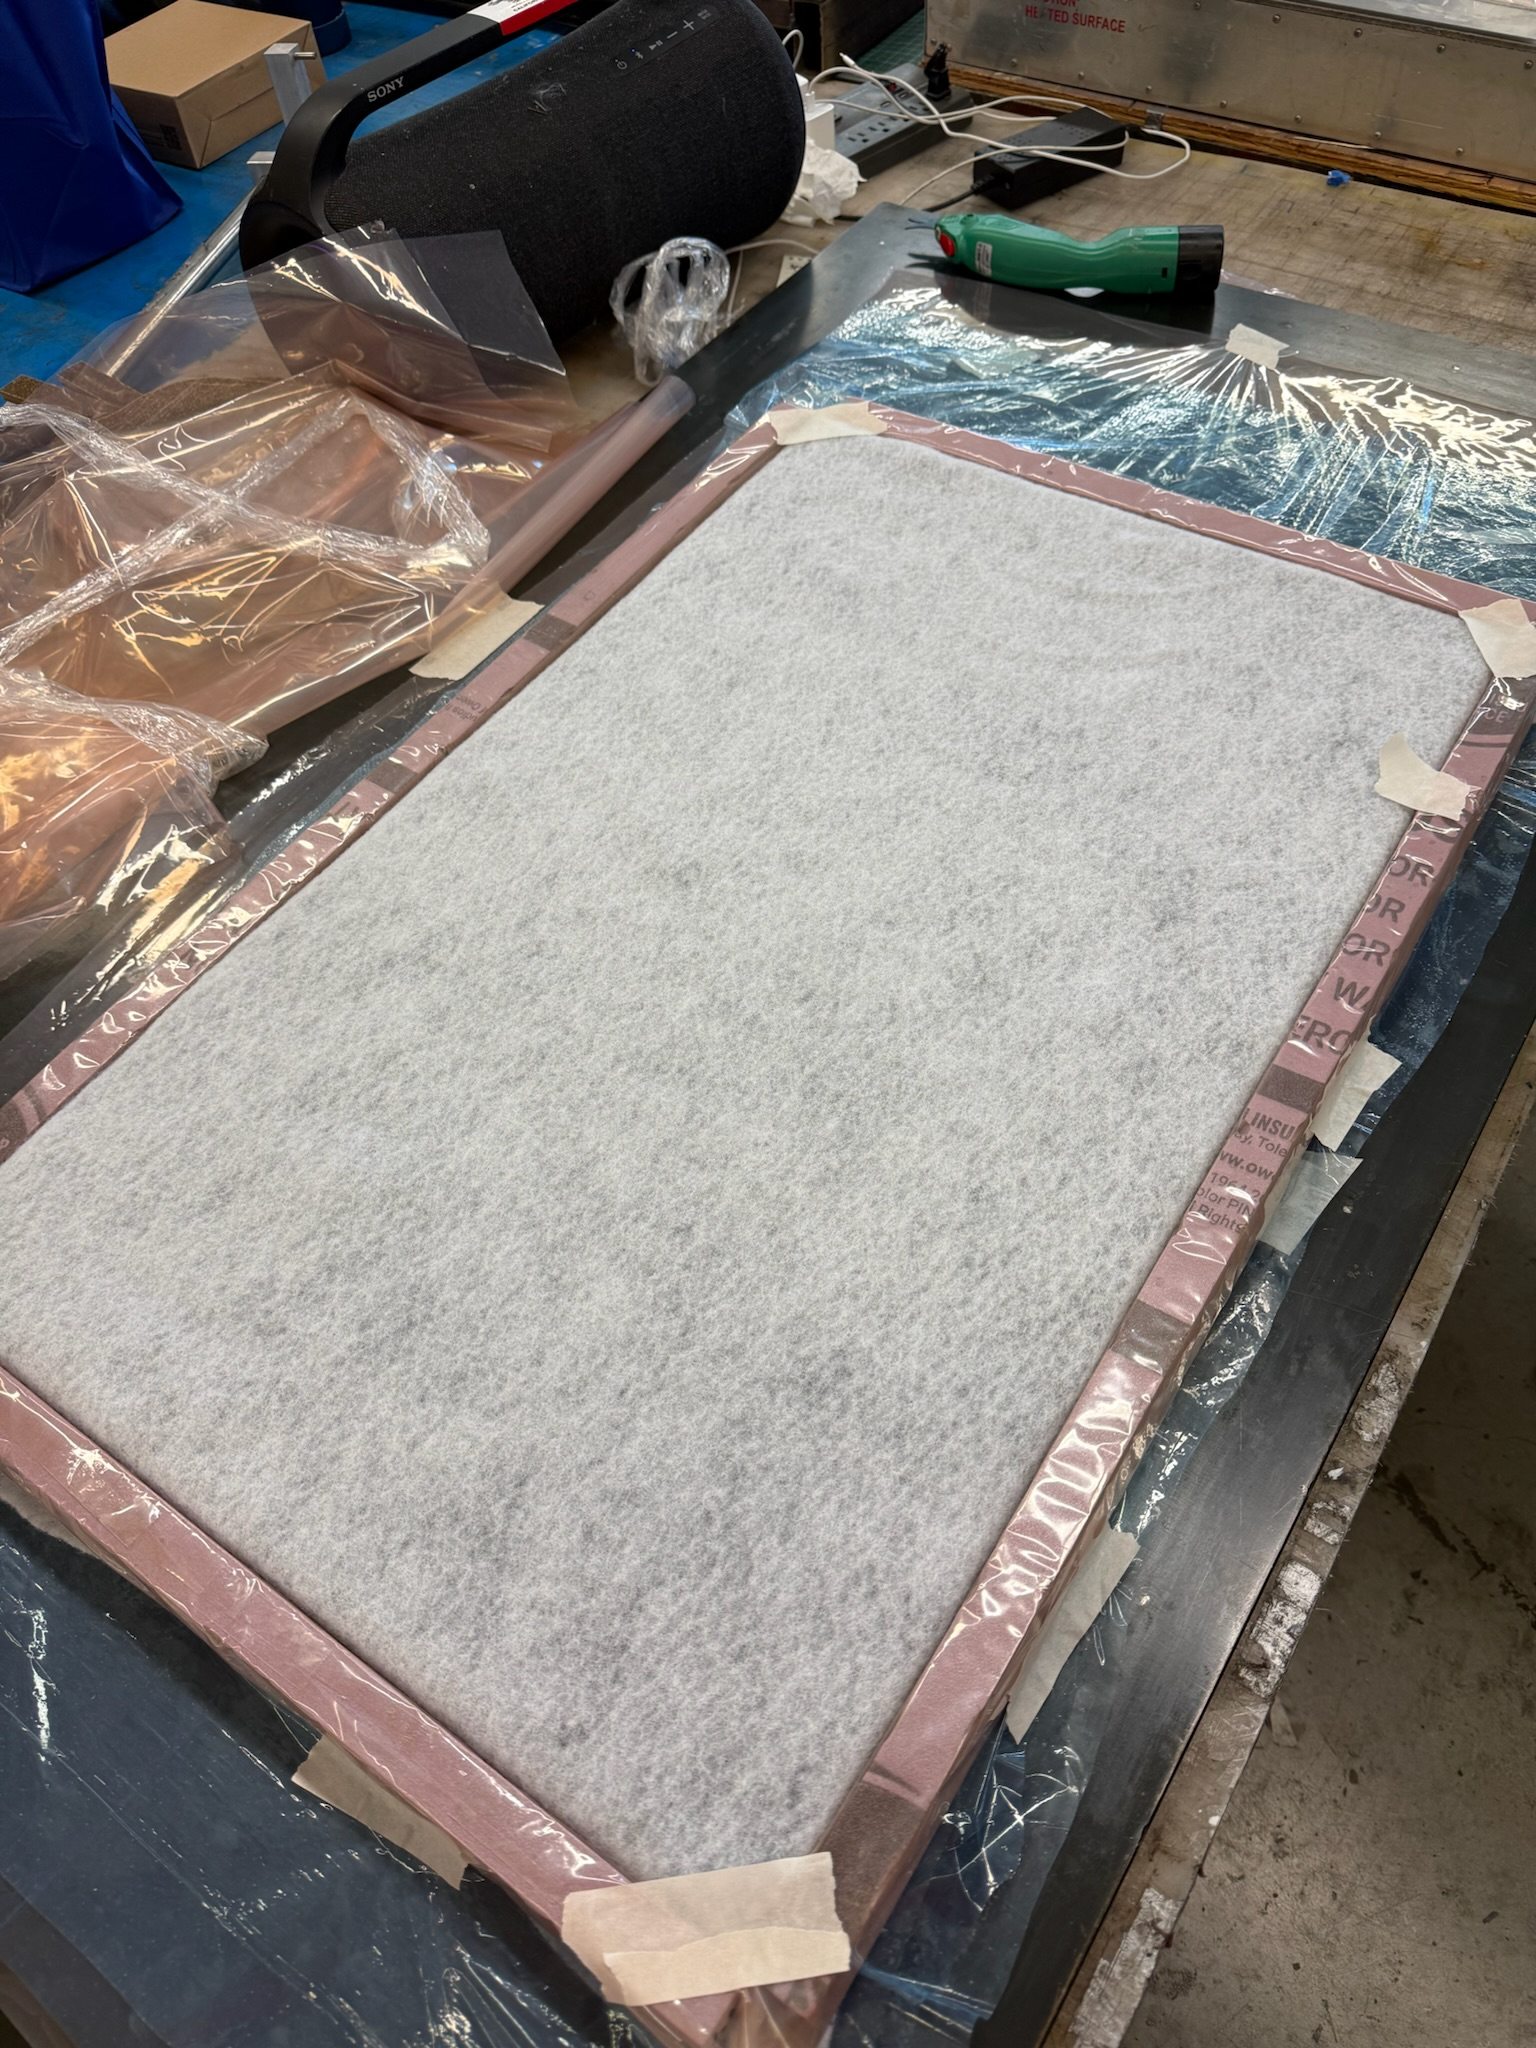
\includegraphics[
        width=3.10in,
        height=1.40in,
        keepaspectratio
    ]{completed_layup}
};
\draw[RuleGray,line width=0.55pt,rounded corners=4pt]
    ($(current page.north west)+(0.43in,-5.13in)$)
    rectangle
    ($(current page.north west)+(3.71in,-6.62in)$);

% Row 2 image 2 — oven chamber used only as a reliable vacuum enclosure; no heat applied
\node[anchor=center,inner sep=0pt]
at ($(current page.north west)+(5.50in,-5.875in)$)
{
    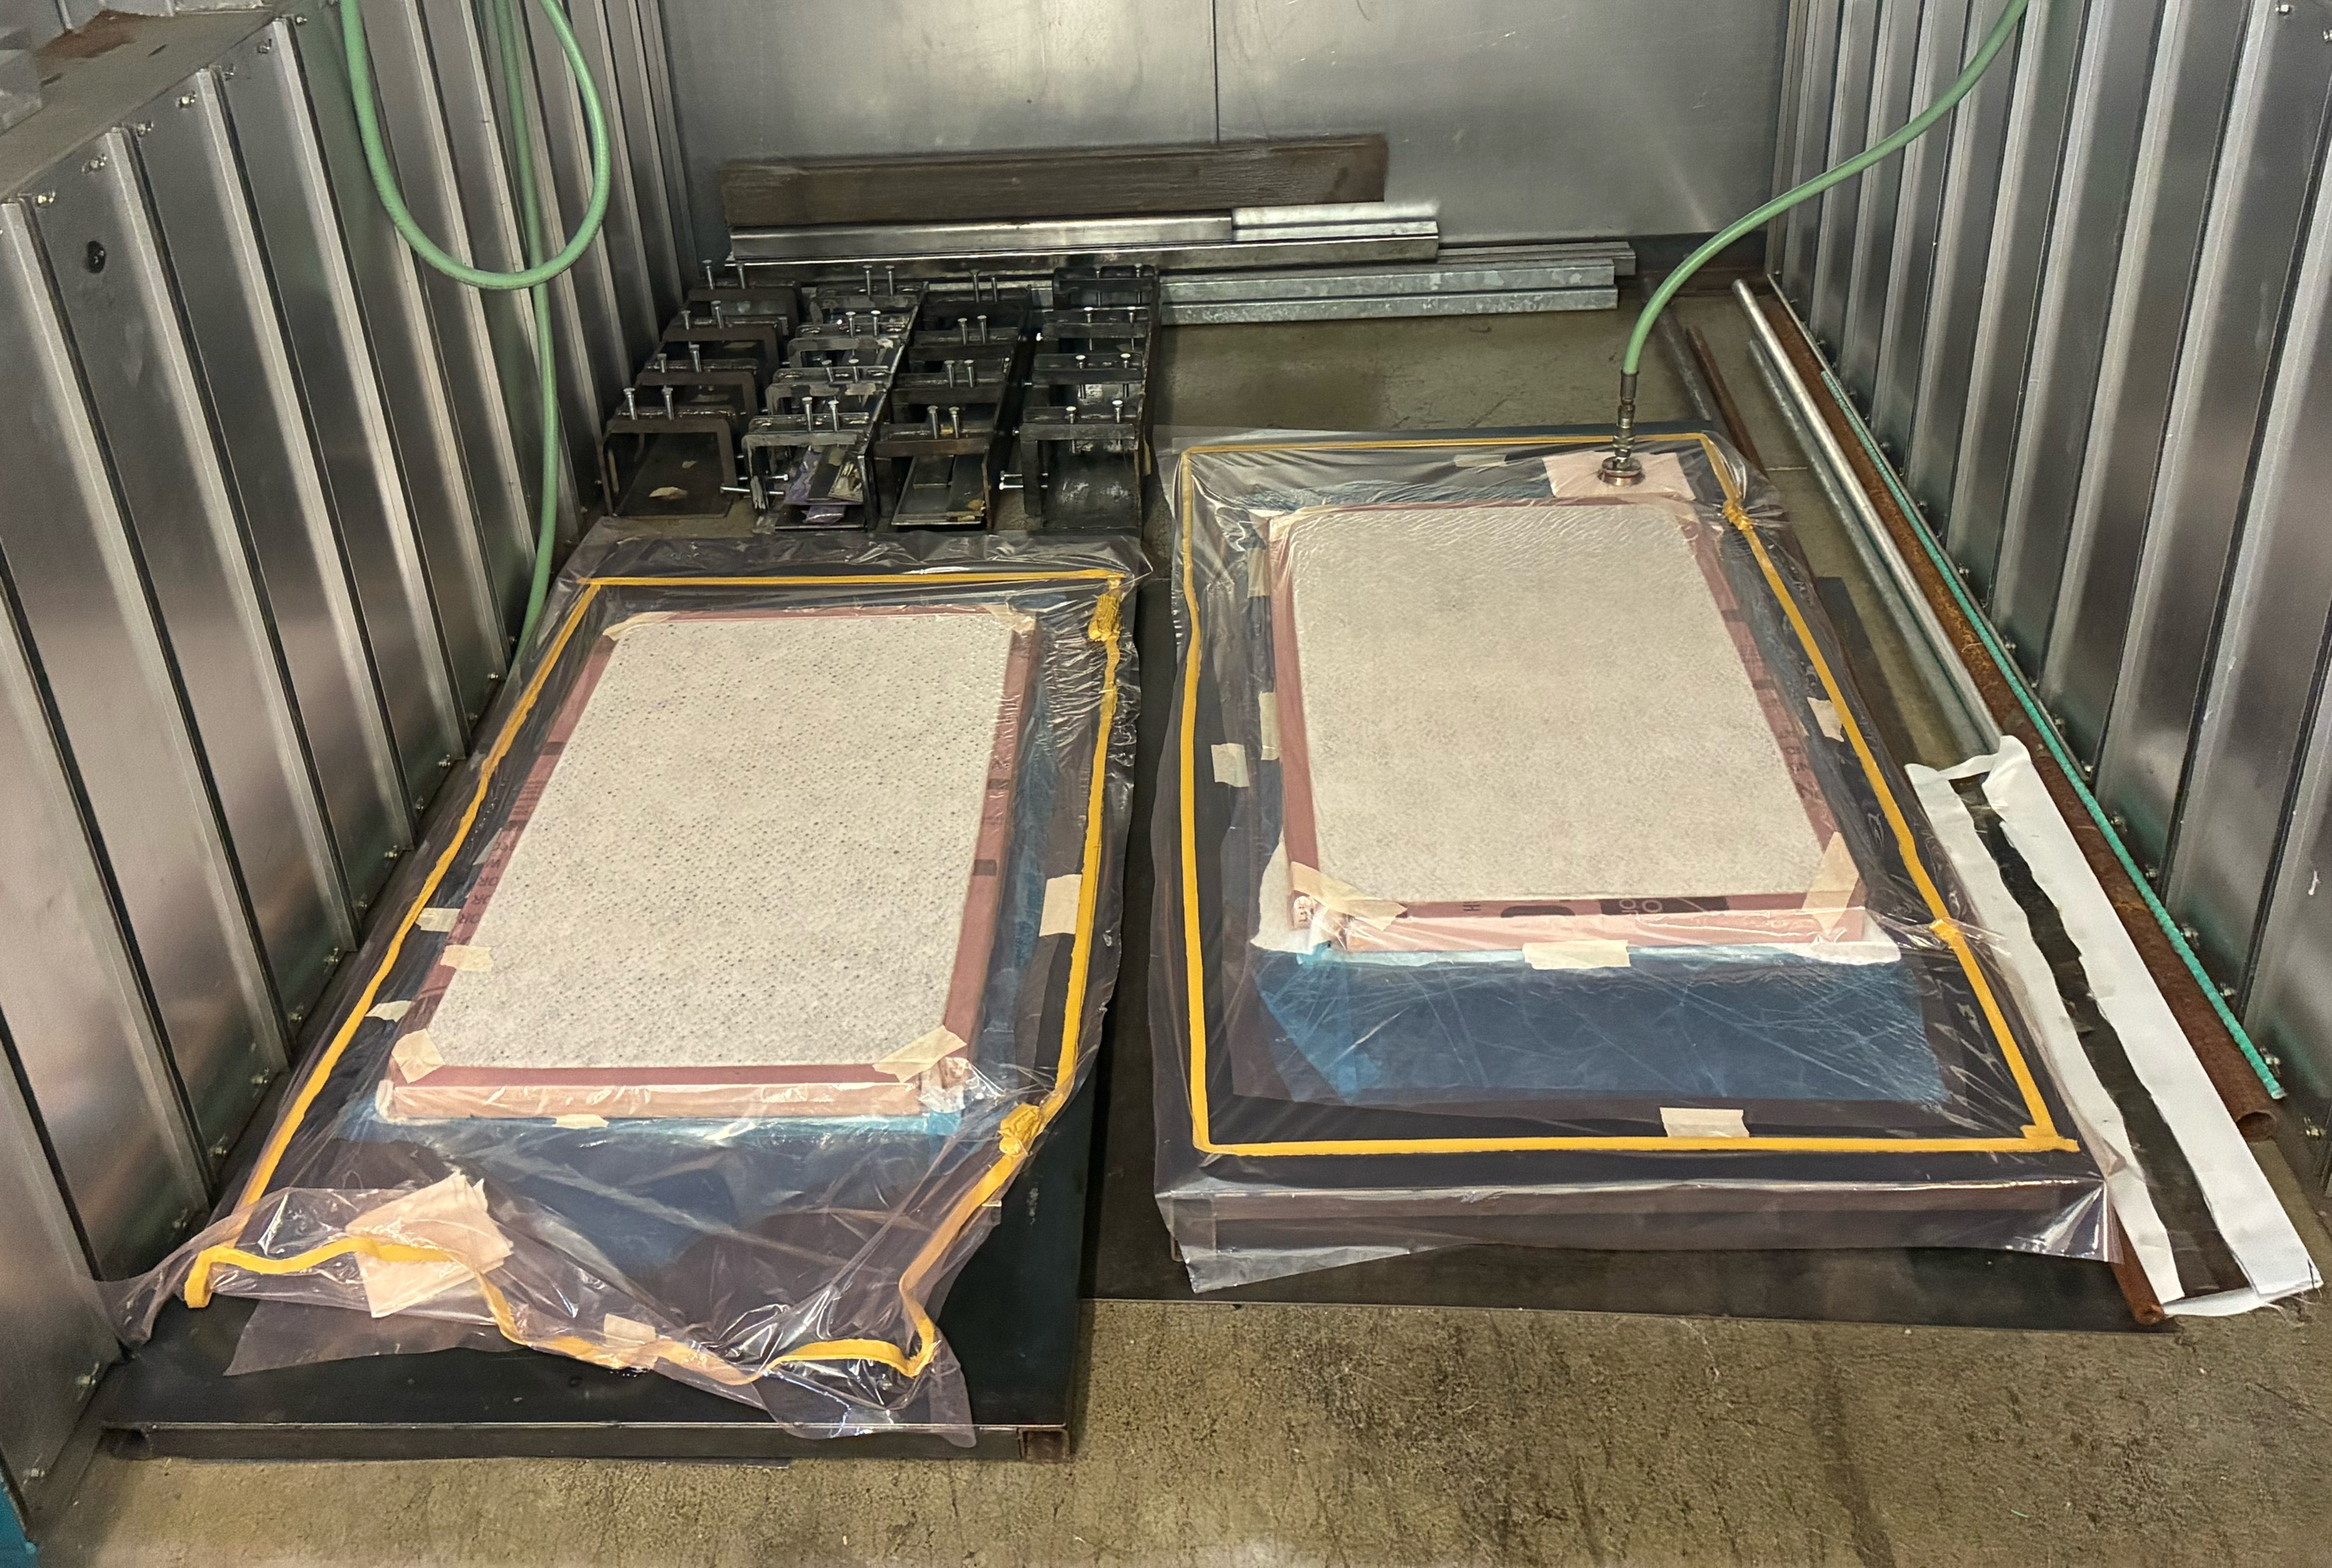
\includegraphics[
        width=3.10in,
        height=1.40in,
        keepaspectratio
    ]{layups_in_composite_oven_under_vacuumPressure}
};
\draw[RuleGray,line width=0.55pt,rounded corners=4pt]
    ($(current page.north west)+(3.86in,-5.13in)$)
    rectangle
    ($(current page.north west)+(7.14in,-6.62in)$);

% Row 2 image 3
\node[anchor=center,inner sep=0pt]
at ($(current page.north west)+(8.935in,-5.875in)$)
{
    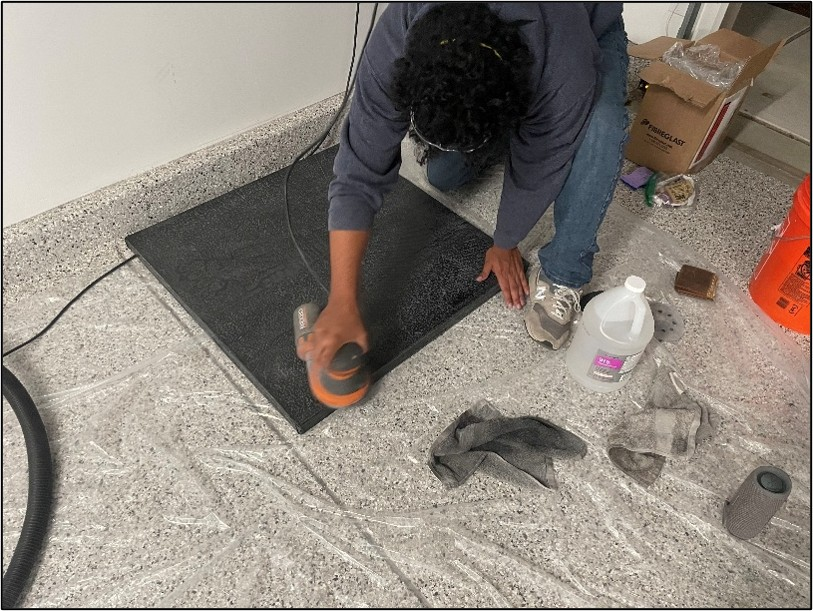
\includegraphics[
        width=3.10in,
        height=1.40in,
        keepaspectratio
    ]{garage_sanding}
};
\draw[RuleGray,line width=0.55pt,rounded corners=4pt]
    ($(current page.north west)+(7.29in,-5.13in)$)
    rectangle
    ($(current page.north east)+(-0.42in,-6.62in)$);

% Row 2 captions
\node[anchor=north,text=Muted,font=\sffamily\fontsize{6.7}{7.3}\selectfont]
at ($(current page.north west)+(2.07in,-6.67in)$)
{4. Fully saturated carbon skin and foam sandwich};

\node[anchor=north,text=Muted,font=\sffamily\fontsize{6.7}{7.3}\selectfont]
at ($(current page.north west)+(5.50in,-6.67in)$)
{5. Room-temperature cure under continuous vacuum};

\node[anchor=north,text=Muted,font=\sffamily\fontsize{6.7}{7.3}\selectfont]
at ($(current page.north west)+(8.935in,-6.67in)$)
{6. Post-processing and surface preparation};

% Bottom callouts
\fill[Panel,rounded corners=4pt]
    ($(current page.north west)+(0.43in,-6.95in)$)
    rectangle
    ($(current page.north west)+(5.48in,-7.60in)$);

\draw[RuleGray,line width=0.55pt,rounded corners=4pt]
    ($(current page.north west)+(0.43in,-6.95in)$)
    rectangle
    ($(current page.north west)+(5.48in,-7.60in)$);

\node[
    anchor=north west,
    text=DeepGreen,
    font=\sffamily\bfseries\fontsize{7.0}{7.6}\selectfont
]
at ($(current page.north west)+(0.63in,-7.08in)$)
{FROM THREE LAYUPS TO ONE};

\node[
    anchor=north west,
    align=left,
    text width=4.56in,
    text=Ink,
    font=\fontsize{6.45}{7.45}\selectfont
]
at ($(current page.north west)+(0.63in,-7.29in)$)
{
The Envelope Method reduced labor, cure cycles, handling,
alignment risk, and time spent forming numerous vacuum-bag
pleats around the 1.5-inch-thick XPS panels.
};

\fill[Panel,rounded corners=4pt]
    ($(current page.north west)+(5.68in,-6.95in)$)
    rectangle
    ($(current page.north east)+(-0.42in,-7.60in)$);

\draw[RuleGray,line width=0.55pt,rounded corners=4pt]
    ($(current page.north west)+(5.68in,-6.95in)$)
    rectangle
    ($(current page.north east)+(-0.42in,-7.60in)$);

\node[
    anchor=north west,
    text=DeepGreen,
    font=\sffamily\bfseries\fontsize{7.0}{7.6}\selectfont
]
at ($(current page.north west)+(5.88in,-7.08in)$)
{WHY SURFACE-BONDED HARDWARE};

\node[
    anchor=north west,
    align=left,
    text width=4.55in,
    text=Ink,
    font=\fontsize{6.45}{7.45}\selectfont
]
at ($(current page.north west)+(5.88in,-7.29in)$)
{
Adhesively bonded hinges and fixtures preserved the clean
composite exterior and avoided drilled inserts, foam-core
crushing, added stress concentrations, and new leak paths.
};


% Footer
\node[
    anchor=south west,
    text=white,
    font=\sffamily\bfseries\fontsize{7.1}{7.7}\selectfont
]
at ($(current page.south west)+(0.42in,0.17in)$)
{\faArrowLeft\ PRODUCT ARCHITECTURE};

\node[
    anchor=south,
    text=white,
    font=\sffamily\fontsize{7.0}{7.6}\selectfont
]
at ($(current page.south)+(0,0.17in)$)
{TORO COVER \hspace{6pt} 2 / 3};

\node[
    anchor=south east,
    text=white,
    font=\sffamily\bfseries\fontsize{7.1}{7.7}\selectfont
]
at ($(current page.south east)+(-0.42in,0.17in)$)
{VALIDATION \& TAKEAWAYS \faArrowRight};

\end{tikzpicture}


% ============================================================
% PAGE 3 — FINISHING, VALIDATION, AND TAKEAWAYS
% ============================================================

\clearpage
\thispagestyle{empty}
\hypertarget{toro-results}{}
\null

\begin{tikzpicture}[remember picture,overlay]

% Background and bars
\fill[white]
    (current page.south west)
    rectangle
    (current page.north east);

\fill[DeepGreen]
    (current page.north west)
    rectangle
    ($(current page.north east)+(0,-0.095in)$);

\fill[PolyGold]
    ($(current page.north west)+(0,-0.095in)$)
    rectangle
    ($(current page.north east)+(0,-0.14in)$);

\fill[DeepGreen]
    (current page.south west)
    rectangle
    ($(current page.south east)+(0,0.36in)$);

\fill[PolyGold]
    ($(current page.south west)+(0,0.36in)$)
    rectangle
    ($(current page.south east)+(0,0.405in)$);

% Header
\node[
    anchor=north west,
    text=PolyGold,
    font=\sffamily\bfseries\fontsize{8.1}{8.7}\selectfont
]
at ($(current page.north west)+(0.42in,-0.39in)$)
{TORO COVER \hspace{5pt}/\hspace{5pt} VALIDATION AND ENGINEERING TAKEAWAYS};

\node[
    anchor=north west,
    text=DeepGreen,
    font=\bfseries\fontsize{22.5}{23.5}\selectfont
]
at ($(current page.north west)+(0.40in,-0.67in)$)
{FROM PROTOTYPE TO PRODUCT PATHWAY};

\node[
    anchor=north west,
    text=Muted,
    font=\sffamily\fontsize{8.7}{9.6}\selectfont
]
at ($(current page.north west)+(0.42in,-1.12in)$)
{Environmental protection, usability testing, scope decisions, and lessons from technical leadership};

\fill[PolyGold]
    ($(current page.north west)+(0.42in,-1.36in)$)
    rectangle
    ($(current page.north west)+(5.8in,-1.315in)$);

% Finishing title
\node[
    anchor=north west,
    text=DeepGreen,
    font=\sffamily\bfseries\fontsize{8.0}{8.7}\selectfont
]
at ($(current page.north west)+(0.43in,-1.62in)$)
{OUTDOOR FINISHING AND ENVIRONMENTAL PROTECTION};

% Image 1
\node[anchor=center,inner sep=0pt]
at ($(current page.north west)+(1.705in,-2.655in)$)
{
    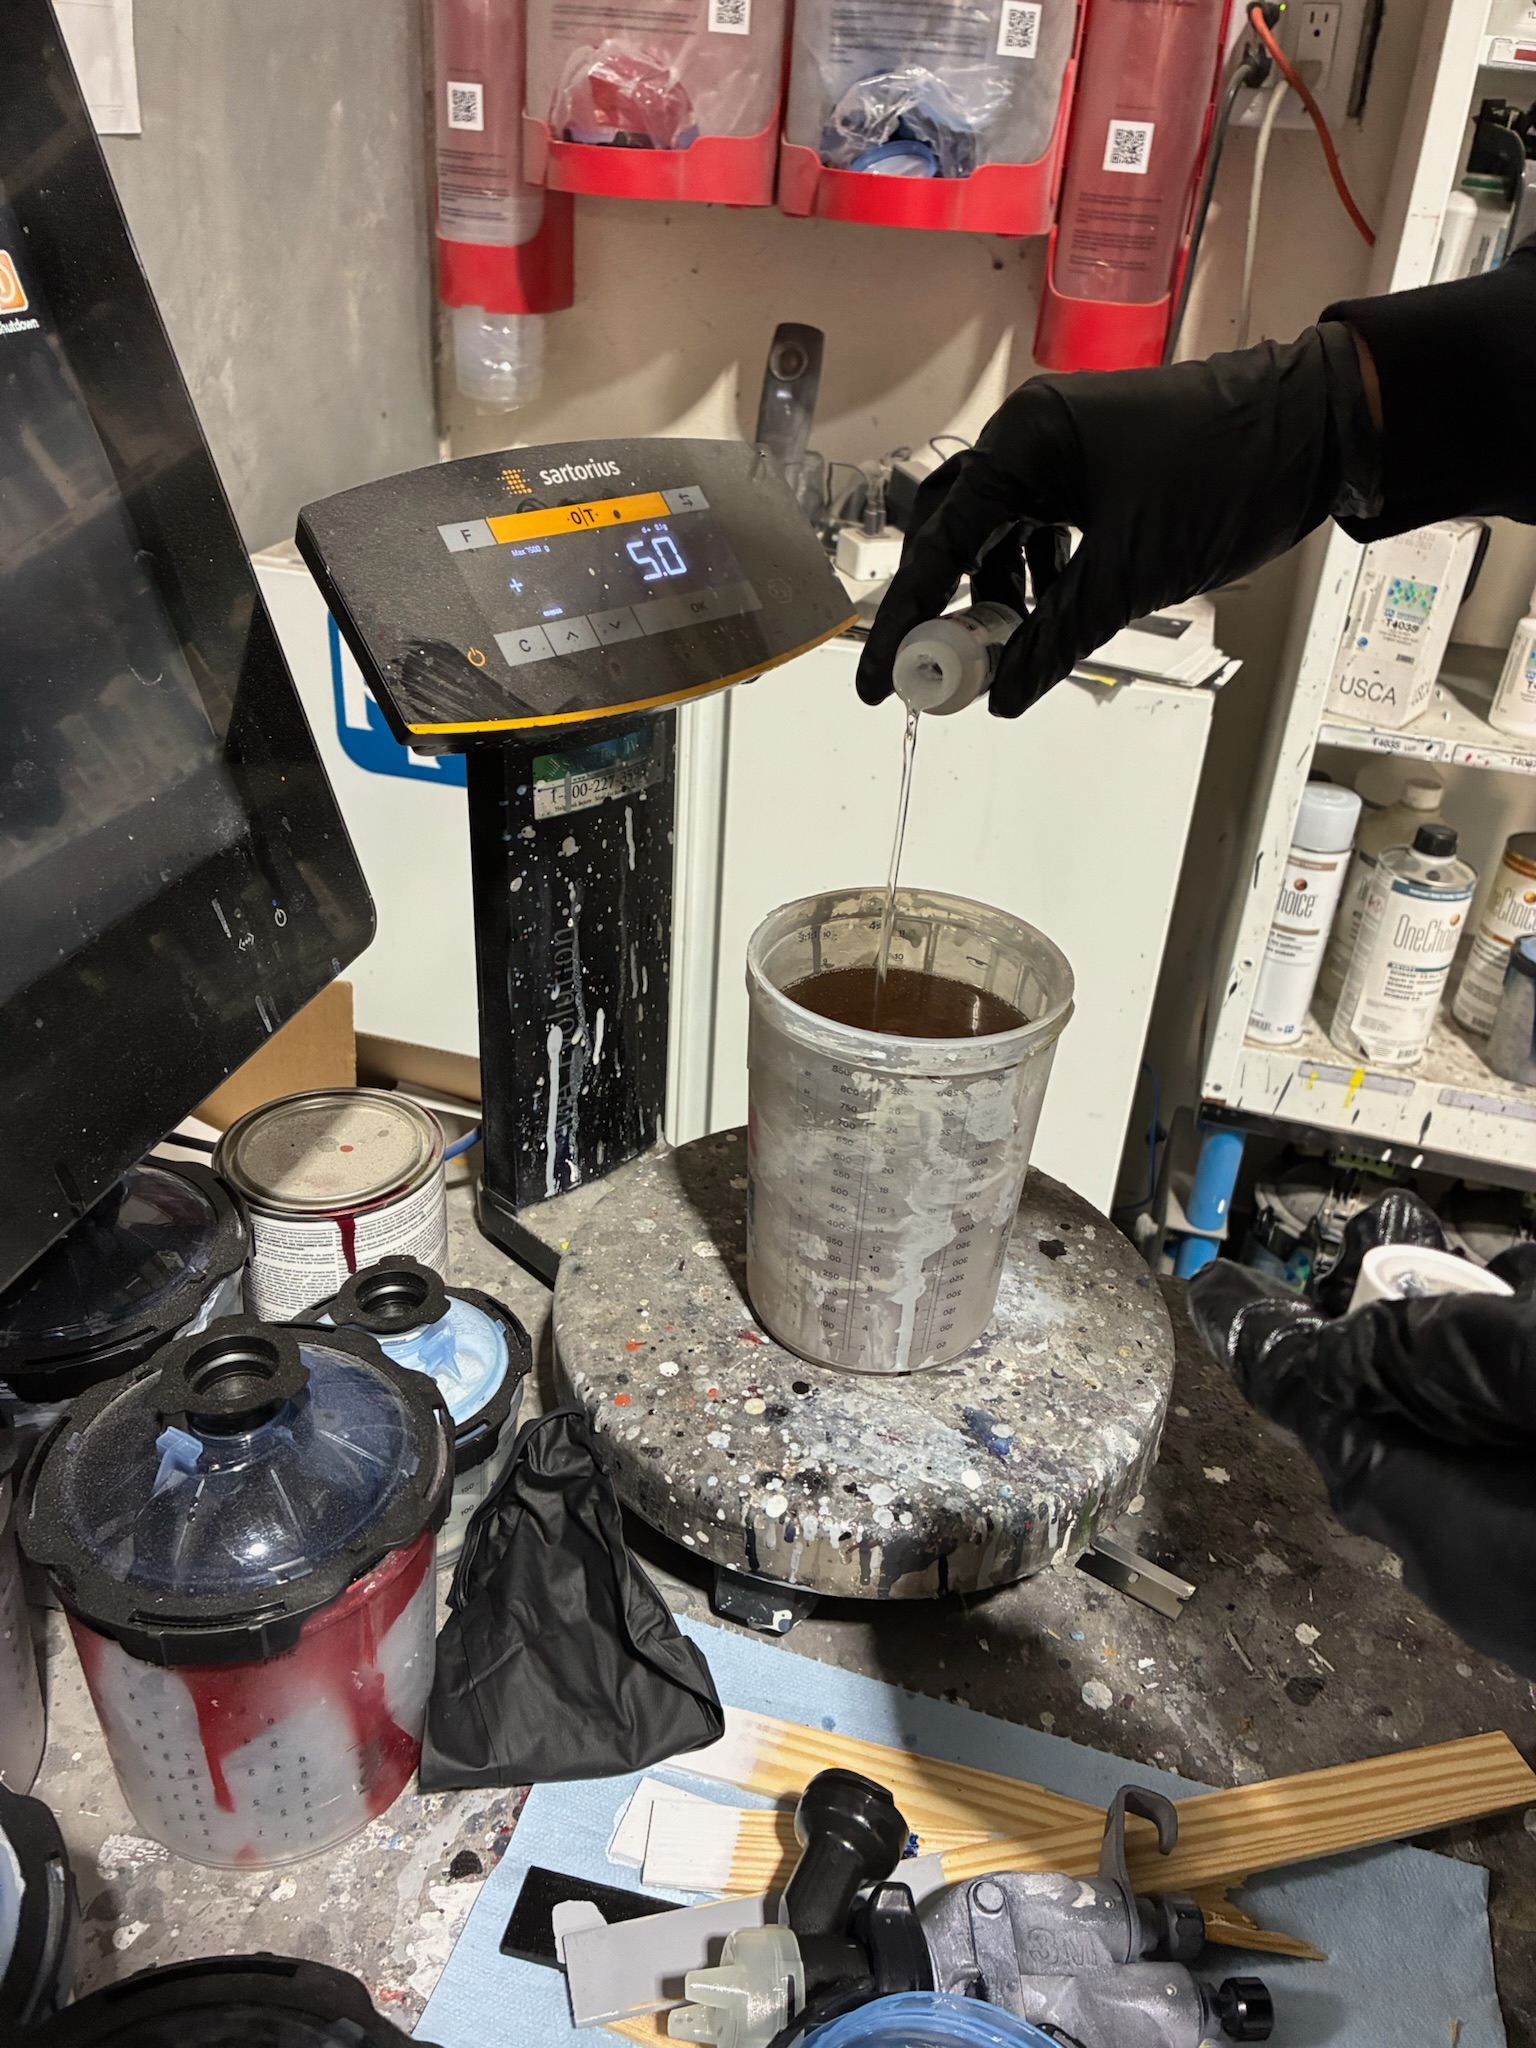
\includegraphics[
        width=2.35in,
        height=1.40in,
        keepaspectratio
    ]{spray_topcoat_prep}
};
\draw[RuleGray,line width=0.55pt,rounded corners=4pt]
    ($(current page.north west)+(0.43in,-1.91in)$)
    rectangle
    ($(current page.north west)+(2.98in,-3.40in)$);

% Image 2
\node[anchor=center,inner sep=0pt]
at ($(current page.north west)+(4.375in,-2.655in)$)
{
    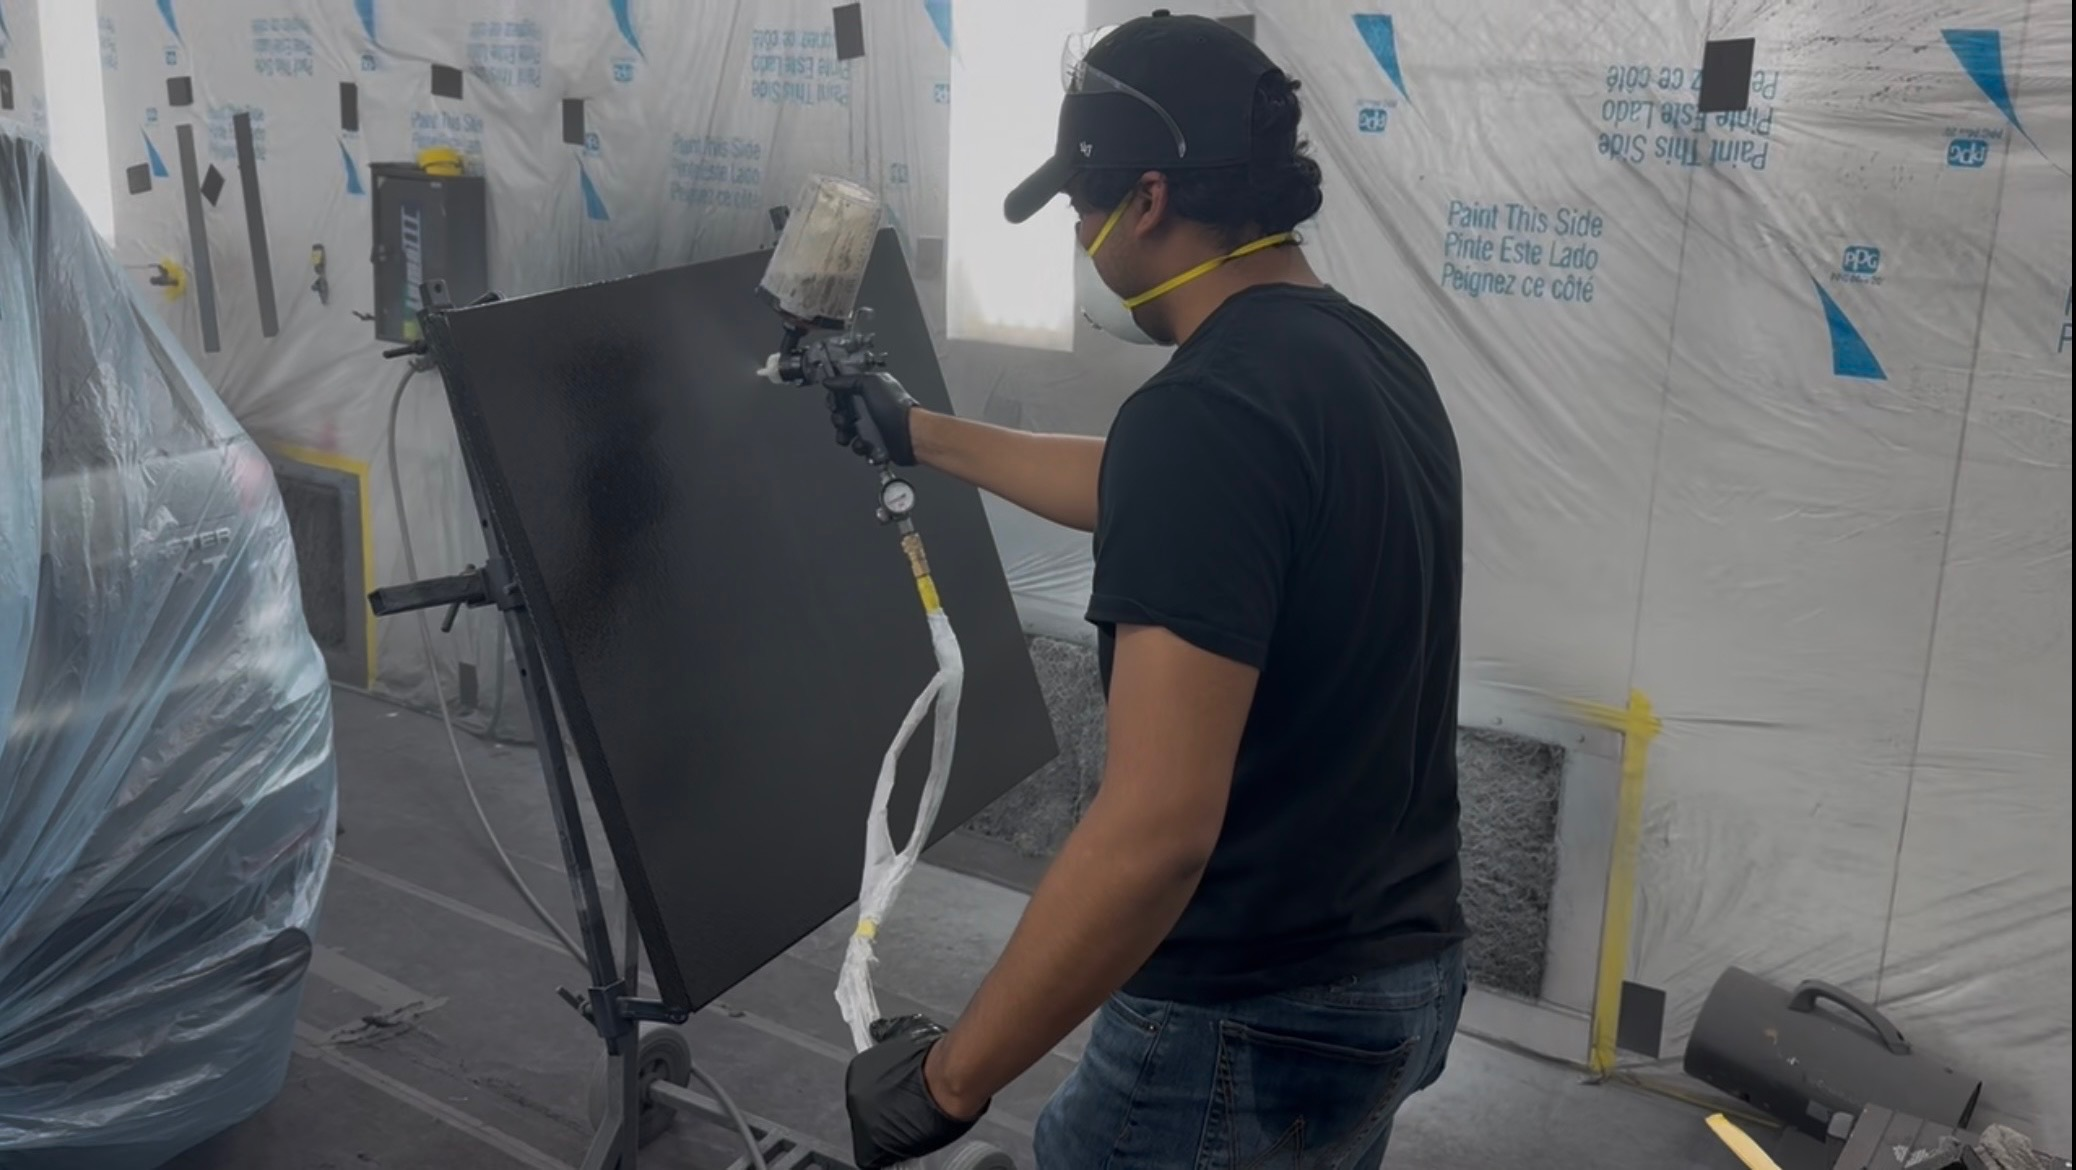
\includegraphics[
        width=2.35in,
        height=1.40in,
        keepaspectratio
    ]{spraying_topcoat}
};
\draw[RuleGray,line width=0.55pt,rounded corners=4pt]
    ($(current page.north west)+(3.10in,-1.91in)$)
    rectangle
    ($(current page.north west)+(5.65in,-3.40in)$);

% Image 3
\node[anchor=center,inner sep=0pt]
at ($(current page.north west)+(7.045in,-2.655in)$)
{
    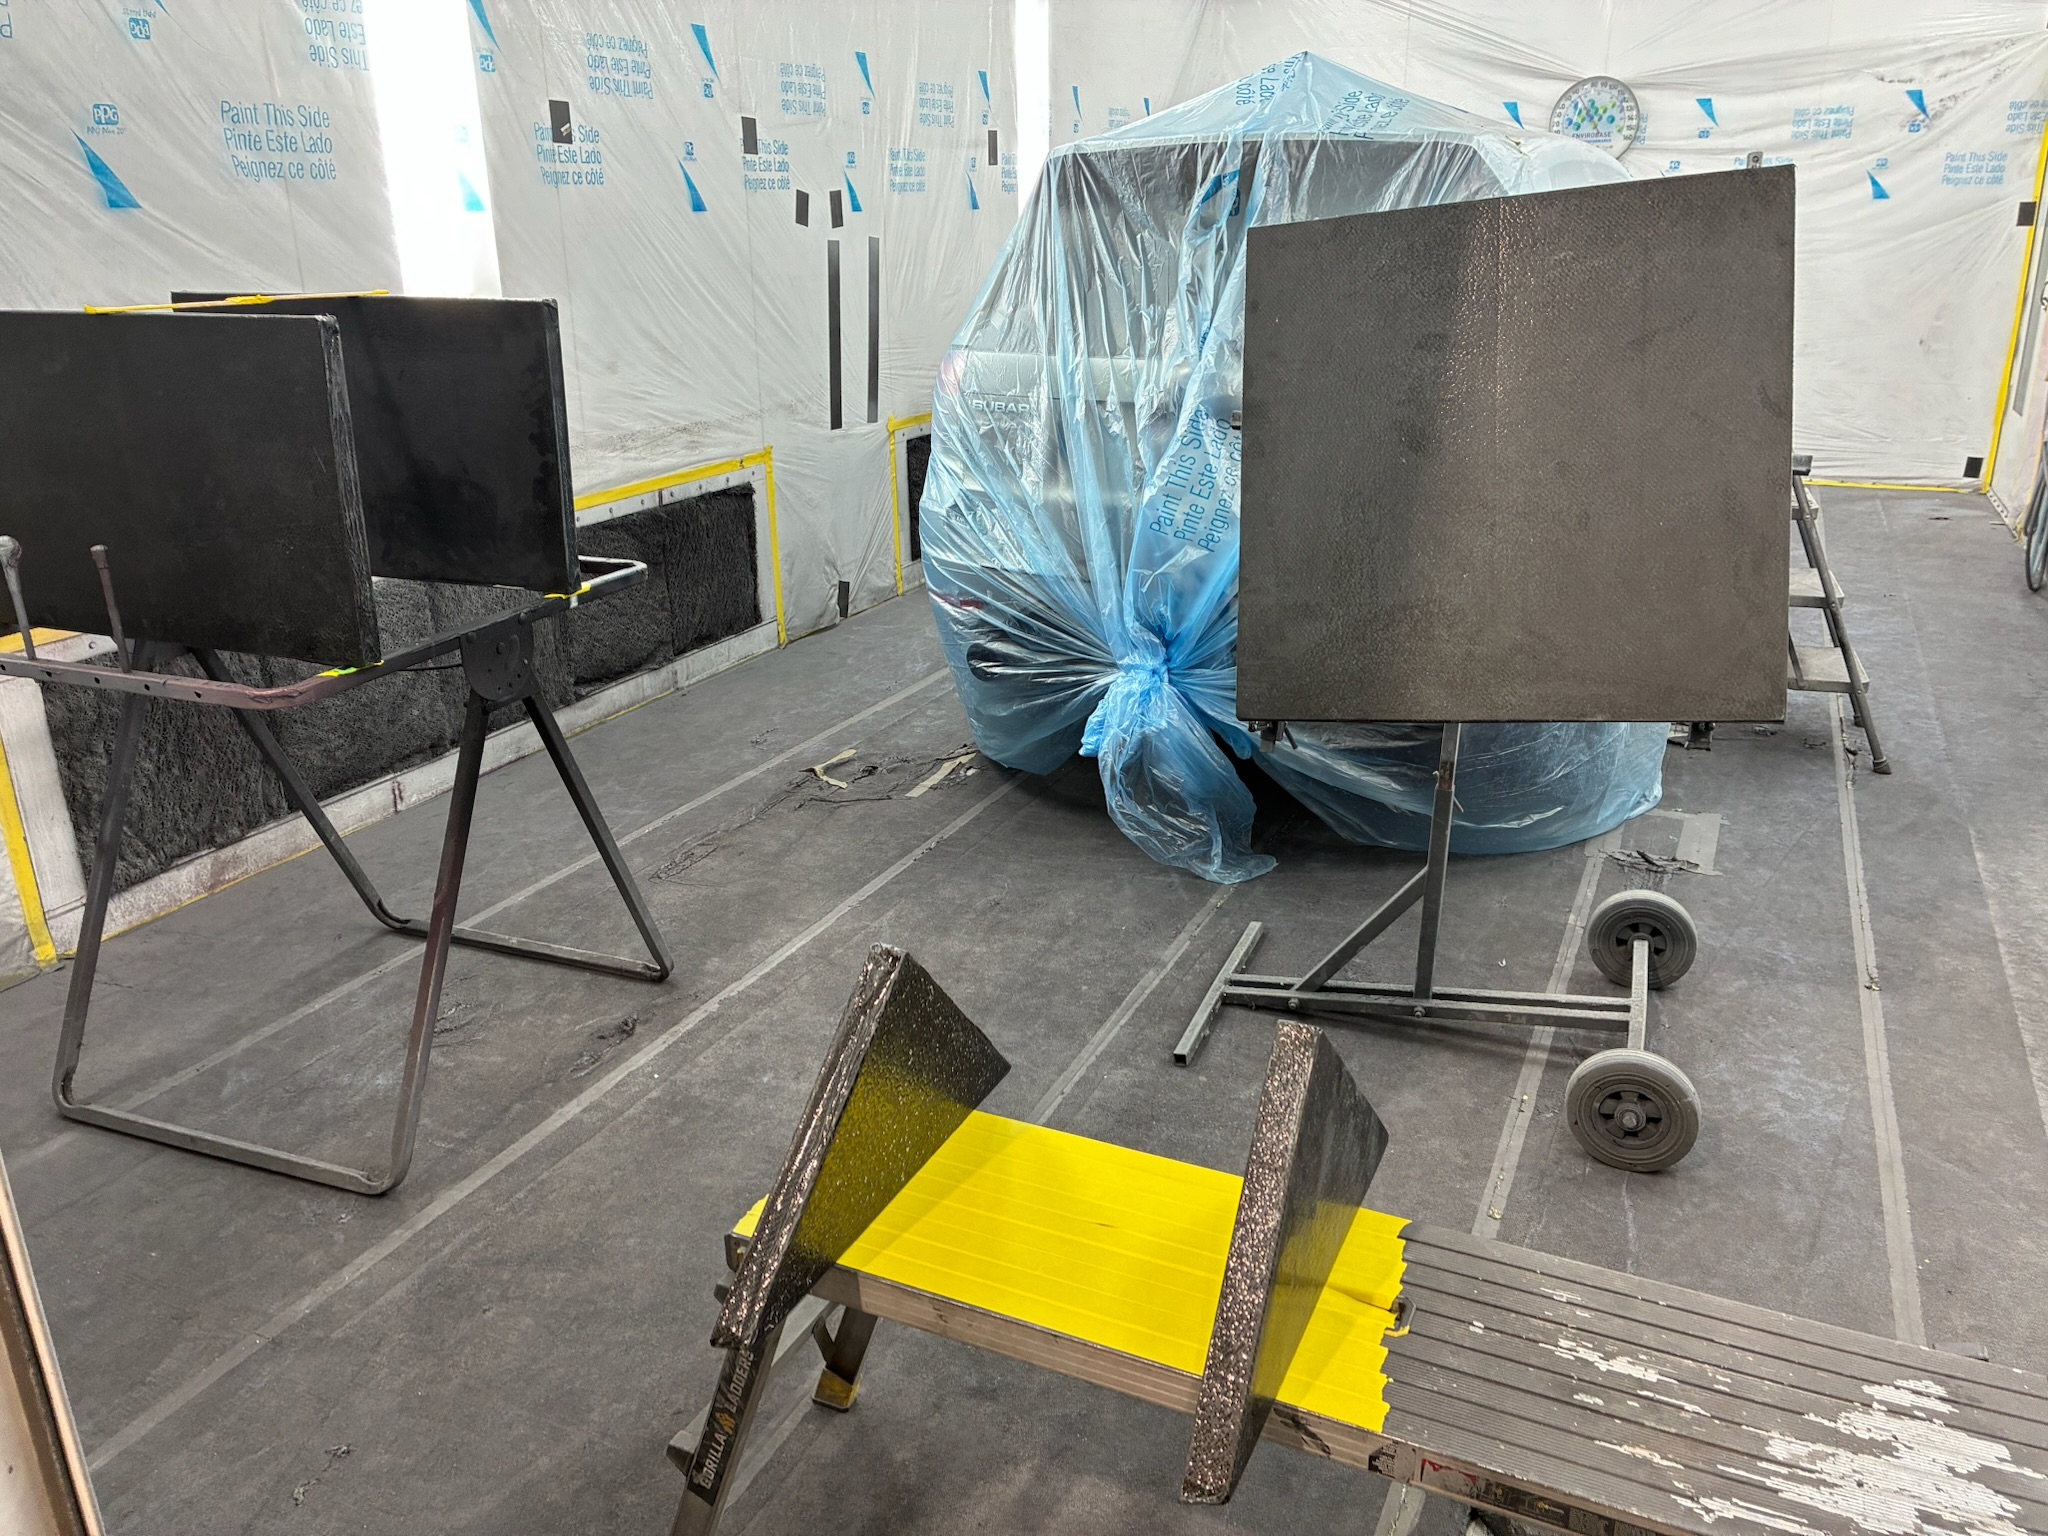
\includegraphics[
        width=2.35in,
        height=1.40in,
        keepaspectratio
    ]{topcoat_setup_apparatus}
};
\draw[RuleGray,line width=0.55pt,rounded corners=4pt]
    ($(current page.north west)+(5.77in,-1.91in)$)
    rectangle
    ($(current page.north west)+(8.32in,-3.40in)$);

% Image 4
\node[anchor=center,inner sep=0pt]
at ($(current page.north west)+(9.50in,-2.655in)$)
{
    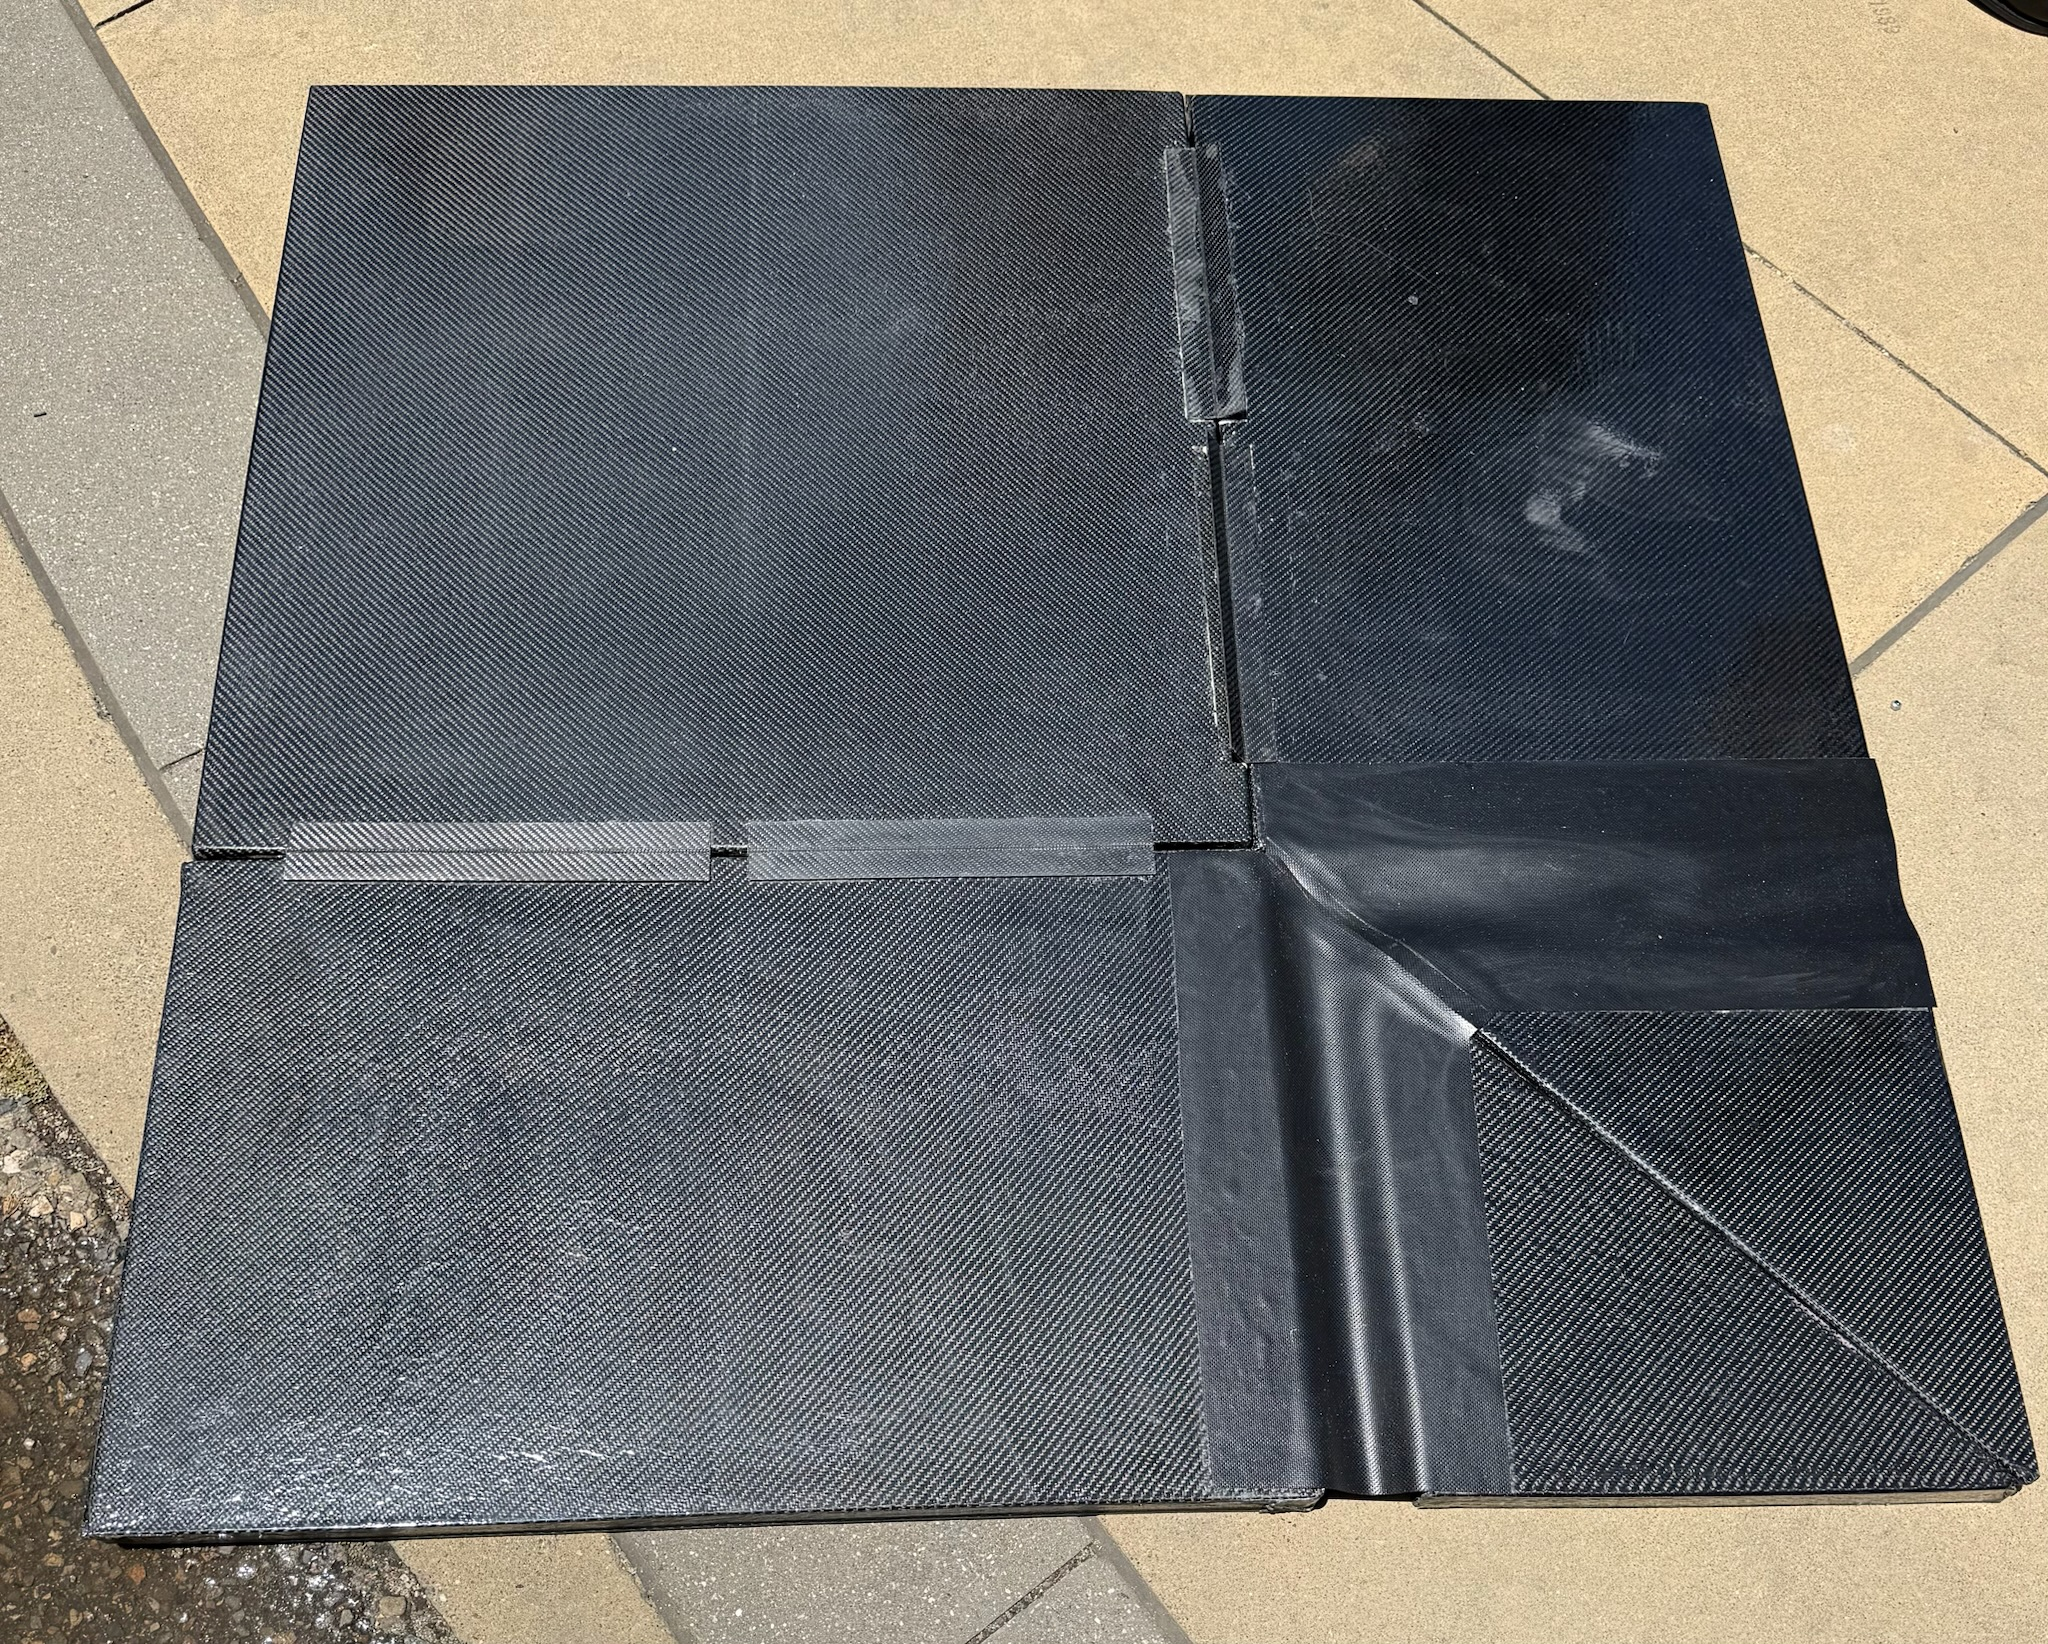
\includegraphics[
        width=2.35in,
        height=1.40in,
        keepaspectratio
    ]{refined_final_toro_cover_partial_carbon_model}
};
\draw[RuleGray,line width=0.55pt,rounded corners=4pt]
    ($(current page.north west)+(8.44in,-1.91in)$)
    rectangle
    ($(current page.north east)+(-0.42in,-3.40in)$);

% Captions
\node[anchor=north,text=Muted,font=\sffamily\fontsize{6.7}{7.3}\selectfont]
at ($(current page.north west)+(1.705in,-3.45in)$)
{Topcoat material preparation};

\node[anchor=north,text=Muted,font=\sffamily\fontsize{6.7}{7.3}\selectfont]
at ($(current page.north west)+(4.375in,-3.45in)$)
{Automotive-booth topcoat application};

\node[anchor=north,text=Muted,font=\sffamily\fontsize{6.7}{7.3}\selectfont]
at ($(current page.north west)+(7.045in,-3.45in)$)
{Coated panels drying after application};

\node[anchor=north,text=Muted,font=\sffamily\fontsize{6.7}{7.3}\selectfont]
at ($(current page.north west)+(9.50in,-3.45in)$)
{Partial carbon manufacturing model};

% Environmental rationale
\fill[SoftGold,rounded corners=4pt]
    ($(current page.north west)+(0.43in,-3.73in)$)
    rectangle
    ($(current page.north east)+(-0.42in,-4.76in)$);

\node[
    anchor=north west,
    align=left,
    text width=9.75in,
    text=Ink,
    font=\fontsize{7.05}{8.25}\selectfont
]
at ($(current page.north west)+(0.65in,-3.89in)$)
{
Because the sponsor required a carbon-fiber cover for outdoor use near chlorinated water,
environmental protection became a functional requirement rather than a cosmetic finish.
I selected and personally sprayed a UV-resistant Sunshield topcoat to seal minor laminate
porosity, reduce moisture ingress, preserve the carbon appearance, limit UV degradation of
the epoxy matrix, and isolate the composite surface from nearby metallic hardware.
};

% Results title
\node[
    anchor=north west,
    text=DeepGreen,
    font=\sffamily\bfseries\fontsize{8.0}{8.7}\selectfont
]
at ($(current page.north west)+(0.43in,-4.94in)$)
{FUNCTIONAL PROTOTYPE RESULTS};

% ------------------------------------------------------------
% Matched lower panels — larger type and improved allocation
% ------------------------------------------------------------

% Left results panel
\fill[SoftGreen,rounded corners=5pt]
    ($(current page.north west)+(0.43in,-5.22in)$)
    rectangle
    ($(current page.north west)+(5.98in,-7.39in)$);

\draw[RuleGray,line width=0.65pt,rounded corners=5pt]
    ($(current page.north west)+(0.43in,-5.22in)$)
    rectangle
    ($(current page.north west)+(5.98in,-7.39in)$);

\fill[DeepGreen,rounded corners=5pt]
    ($(current page.north west)+(0.43in,-5.22in)$)
    rectangle
    ($(current page.north west)+(5.98in,-5.58in)$);

\fill[DeepGreen]
    ($(current page.north west)+(0.43in,-5.40in)$)
    rectangle
    ($(current page.north west)+(5.98in,-5.58in)$);

\node[anchor=west,text=white,
      font=\sffamily\bfseries\fontsize{7.0}{7.6}\selectfont]
at ($(current page.north west)+(0.66in,-5.40in)$)
{SPECIFICATION};

\node[anchor=west,text=white,
      font=\sffamily\bfseries\fontsize{7.0}{7.6}\selectfont]
at ($(current page.north west)+(3.02in,-5.40in)$)
{RESULT};

\node[anchor=east,text=white,
      font=\sffamily\bfseries\fontsize{7.0}{7.6}\selectfont]
at ($(current page.north west)+(5.55in,-5.40in)$)
{STATUS};

\node[
    anchor=north west,
    align=left,
    text width=2.15in,
    text=Ink,
    font=\bfseries\fontsize{7.15}{8.55}\selectfont
]
at ($(current page.north west)+(0.66in,-5.72in)$)
{
Deployment time\\[3.4pt]
Removal time\\[3.4pt]
Single-user operation\\[3.4pt]
Single-side operation\\[3.4pt]
Deployment steps\\[3.4pt]
Removal steps\\[3.4pt]
Weight\\[3.4pt]
Folded storage
};

\node[
    anchor=north west,
    align=left,
    text width=1.45in,
    text=Ink,
    font=\fontsize{7.15}{8.55}\selectfont
]
at ($(current page.north west)+(3.02in,-5.72in)$)
{
25.51 seconds\\[3.4pt]
37.22 seconds\\[3.4pt]
100\% successful\\[3.4pt]
75\% successful\\[3.4pt]
6.4 average\\[3.4pt]
9 average\\[3.4pt]
17 lb\\[3.4pt]
2.9' x 2.9' x 1.7'
};

\node[
    anchor=north east,
    align=right,
    text width=1.05in,
    text=DeepGreen,
    font=\sffamily\bfseries\fontsize{7.05}{8.55}\selectfont
]
at ($(current page.north west)+(5.55in,-5.72in)$)
{
PASS\\[3.4pt]
PASS\\[3.4pt]
PASS\\[3.4pt]
NEAR TARGET\\[3.4pt]
PASS\\[3.4pt]
PASS\\[3.4pt]
NEAR TARGET\\[3.4pt]
PASS
};

% Right takeaways panel — widened for easier reading
\fill[SoftGreen,rounded corners=5pt]
    ($(current page.north west)+(6.14in,-5.22in)$)
    rectangle
    ($(current page.north east)+(-0.42in,-7.39in)$);

\draw[RuleGray,line width=0.65pt,rounded corners=5pt]
    ($(current page.north west)+(6.14in,-5.22in)$)
    rectangle
    ($(current page.north east)+(-0.42in,-7.39in)$);

\fill[DeepGreen,rounded corners=5pt]
    ($(current page.north west)+(6.14in,-5.22in)$)
    rectangle
    ($(current page.north east)+(-0.42in,-5.58in)$);

\fill[DeepGreen]
    ($(current page.north west)+(6.14in,-5.40in)$)
    rectangle
    ($(current page.north east)+(-0.42in,-5.58in)$);

\node[anchor=west,text=white,
      font=\sffamily\bfseries\fontsize{7.1}{7.7}\selectfont]
at ($(current page.north west)+(6.38in,-5.40in)$)
{ENGINEERING TAKEAWAYS};

\node[
    anchor=north west,
    align=left,
    text width=4.02in,
    text=Ink,
    font=\fontsize{6.75}{7.85}\selectfont
]
at ($(current page.north west)+(6.38in,-5.72in)$)
{
\textbf{Manufacturing first.}
Composite manufacturing constraints should guide the product architecture from the beginning.\\[4.5pt]
\textbf{Prioritize deliberately.}
Competing requirements must be balanced intentionally instead of maximizing every objective.\\[4.5pt]
\textbf{Lead through the process.}
Clear procedures, calm communication, and respect for teammates' strengths were essential during fabrication.\\[4.5pt]
\textbf{Next iteration.}
Reduce weight, refine the fabric-hinge fold lines, and improve panel-edge clearance.
};

% Compact concluding pathway
\node[
    anchor=center,
    align=center,
    text=PolyGold,
    font=\sffamily\bfseries\fontsize{6.3}{6.9}\selectfont
]
at ($(current page.north)+(3.06in,-7.18in)$)
{PROTOTYPE \faArrowRight\ DESIGN REFINEMENT
\faArrowRight\ REPEATABLE MANUFACTURING
\faArrowRight\ PRODUCT};

% Validation resources
\node[
    anchor=north,
    align=center,
    text=DeepGreen,
    font=\sffamily\bfseries\fontsize{6.6}{7.2}\selectfont
]
at ($(current page.north)+(0,-7.58in)$)
{\href{\ToroDeploymentLink}{\faPlayCircle\ DEPLOYMENT}
\hspace{18pt}
\href{\ToroRemovalLink}{\faPlayCircle\ REMOVAL / FOLDING}
\hspace{18pt}
\href{\ToroPosterLink}{\faFilePdf\ EXPO POSTER}
\hspace{18pt}
\href{\ToroReportLink}{\faFilePdf\ FINAL REPORT}};

% Footer
\node[
    anchor=south west,
    text=white,
    font=\sffamily\bfseries\fontsize{7.1}{7.7}\selectfont
]
at ($(current page.south west)+(0.42in,0.17in)$)
{\faArrowLeft\ MANUFACTURING-DRIVEN DESIGN};

\node[
    anchor=south,
    text=white,
    font=\sffamily\fontsize{7.0}{7.6}\selectfont
]
at ($(current page.south)+(0,0.17in)$)
{TORO COVER \hspace{6pt} 3 / 3};

\node[
    anchor=south east,
    text=white,
    font=\sffamily\bfseries\fontsize{7.1}{7.7}\selectfont
]
at ($(current page.south east)+(-0.42in,0.17in)$)
{NEXT PROJECT \faArrowRight};

\end{tikzpicture}
\input{paddle}
\clearpage
 before \end{document}.
% 3. Image references use the original Overleaf base filenames
%    without extensions.
% ============================================================



% ============================================================
% CLICKABLE PROJECT RESOURCES
% All links use the exact Google Drive resources supplied.
% ============================================================
\providecommand{\ToroDrawingLink}{https://drive.google.com/file/d/1A7-7wMnRNLuQDaTgxeuUCBsGNqyXzOGV/view?usp=sharing}
\providecommand{\ToroDimensionsLink}{https://drive.google.com/file/d/13sw3BNJvE8GdzlRffxoF2n5r9Gzxide7/view?usp=sharing}
\providecommand{\ToroProblemLink}{https://drive.google.com/file/d/1zHtl8zrb13F1yeN74ptawpfS5UM_xsuw/view?usp=drive_link}
\providecommand{\ToroReportLink}{https://drive.google.com/file/d/1ULZ-P46lFsC2x29ZfmRVIKgYnr9o8hMt/view?usp=drive_link}
\providecommand{\ToroPosterLink}{https://drive.google.com/file/d/1vKiKaJUcHQb_db-FkZnRF6EvtuM4hKyS/view?usp=drive_link}
\providecommand{\ToroDeploymentLink}{https://drive.google.com/file/d/1XJx34o80_mZPTl7xy93HtWAgtS3ThhvY/view?usp=drive_link}
\providecommand{\ToroRemovalLink}{https://drive.google.com/file/d/1O7xYeyB67NUwT-j1B1HeiCcHnZDYjk6_/view?usp=drive_link}

% ============================================================
% PAGE 1 — PROJECT OVERVIEW, OWNERSHIP, AND ARCHITECTURE
% ============================================================

\clearpage
\thispagestyle{empty}
\hypertarget{toro}{}
\null

\begin{tikzpicture}[remember picture,overlay]

% Background
\fill[white]
    (current page.south west)
    rectangle
    (current page.north east);

% Page bars
\fill[DeepGreen]
    (current page.north west)
    rectangle
    ($(current page.north east)+(0,-0.095in)$);

\fill[PolyGold]
    ($(current page.north west)+(0,-0.095in)$)
    rectangle
    ($(current page.north east)+(0,-0.14in)$);

\fill[DeepGreen]
    (current page.south west)
    rectangle
    ($(current page.south east)+(0,0.36in)$);

\fill[PolyGold]
    ($(current page.south west)+(0,0.36in)$)
    rectangle
    ($(current page.south east)+(0,0.405in)$);

% Header
\node[
    anchor=north west,
    text=PolyGold,
    font=\sffamily\bfseries\fontsize{8.1}{8.7}\selectfont
]
at ($(current page.north west)+(0.42in,-0.39in)$)
{01 COMPOSITES \hspace{5pt}/\hspace{5pt} PROJECT 01};

\node[
    anchor=north west,
    text=DeepGreen,
    font=\bfseries\fontsize{23.5}{24.5}\selectfont
]
at ($(current page.north west)+(0.40in,-0.67in)$)
{TORO CARBON FIBER SAFETY COVER};

\node[
    anchor=north west,
    text=Muted,
    font=\sffamily\fontsize{8.4}{9.2}\selectfont
]
at ($(current page.north west)+(0.42in,-1.12in)$)
{Cal Poly Composites Laboratory \hspace{7pt}\textbullet\hspace{7pt}
Team Project \hspace{7pt}\textbullet\hspace{7pt}
Fall--Spring 2026 \hspace{7pt}\textbullet\hspace{7pt}
San Luis Obispo, California};

\fill[PolyGold]
    ($(current page.north west)+(0.42in,-1.37in)$)
    rectangle
    ($(current page.north west)+(6.1in,-1.325in)$);

% Challenge text
\node[
    anchor=north west,
    text=DeepGreen,
    font=\sffamily\bfseries\fontsize{8.1}{8.8}\selectfont
]
at ($(current page.north west)+(0.43in,-1.61in)$)
{THE CHALLENGE};

\node[
    anchor=north west,
    align=left,
    text width=4.47in,
    text=Ink,
    font=\fontsize{8.05}{9.65}\selectfont
]
at ($(current page.north west)+(0.43in,-1.84in)$)
{
Develop a lightweight cover for a 6 ft by 6 ft in-ground spa
that could be deployed by one person, stored compactly,
provide insulation, resist a poolside environment, and maintain
a refined appearance. The sponsor supplied an ambitious but
intentionally broad project statement, requiring the team to
define the product architecture, priorities, manufacturing
strategy, and realistic path toward future commercialization.
};

% Role box
\fill[SoftGold,rounded corners=5pt]
    ($(current page.north west)+(0.42in,-2.88in)$)
    rectangle
    ($(current page.north west)+(4.98in,-4.58in)$);

\fill[PolyGold]
    ($(current page.north west)+(0.42in,-2.88in)$)
    rectangle
    ($(current page.north west)+(0.52in,-4.58in)$);

\node[
    anchor=north west,
    text=DeepGreen,
    font=\sffamily\bfseries\fontsize{8.1}{8.8}\selectfont
]
at ($(current page.north west)+(0.66in,-3.02in)$)
{MY ROLE — DESIGN \& MANUFACTURING LEAD};

\node[
    anchor=north west,
    align=left,
    text width=4.02in,
    text=Ink,
    font=\fontsize{7.05}{8.15}\selectfont
]
at ($(current page.north west)+(0.66in,-3.27in)$)
{
\textbullet\ Modeled every custom part and the complete assembly\\[1.5pt]
\textbullet\ Produced the engineering drawing package independently\\[1.5pt]
\textbullet\ Developed the composite-panel manufacturing process\\[1.5pt]
\textbullet\ Created all waterjet DXFs and manufacturing geometry\\[1.5pt]
\textbullet\ Trained teammates in wet layup and vacuum bagging\\[1.5pt]
\textbullet\ Presented feasibility, scope, and tradeoffs to the sponsor
};

% Large deployed foam-model image
\node[anchor=center,inner sep=0pt]
at ($(current page.north west)+(8.00in,-3.04in)$)
{
    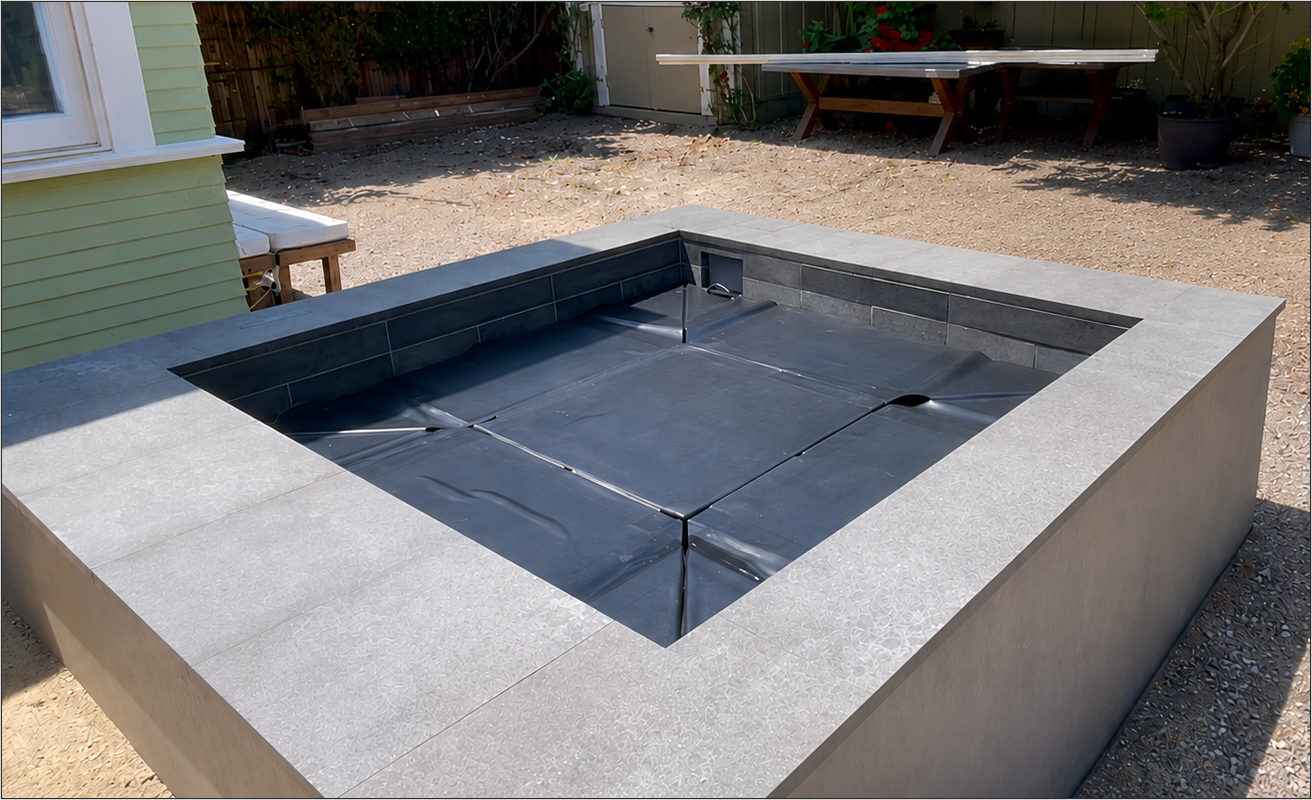
\includegraphics[
        width=5.55in,
        height=2.78in,
        keepaspectratio
    ]{deployed_functional_prototype}
};

\draw[DeepGreen,line width=0.8pt,rounded corners=7pt]
    ($(current page.north west)+(5.16in,-1.61in)$)
    rectangle
    ($(current page.north east)+(-0.42in,-4.47in)$);

\node[
    anchor=north west,
    text=Muted,
    font=\sffamily\fontsize{6.2}{6.9}\selectfont
]
at ($(current page.north west)+(5.18in,-4.54in)$)
{Functional foam model deployed over the sponsor's in-ground spa.};

% Image-strip title
\node[
    anchor=north west,
    text=DeepGreen,
    font=\sffamily\bfseries\fontsize{8.1}{8.8}\selectfont
]
at ($(current page.north west)+(0.43in,-4.78in)$)
{PRODUCT DEVELOPMENT AND FINAL ARCHITECTURE};

% Five-image development strip — CAD-first sequence
% Image 1: topside CAD
\node[anchor=center,inner sep=0pt]
at ($(current page.north west)+(1.47in,-5.73in)$)
{
    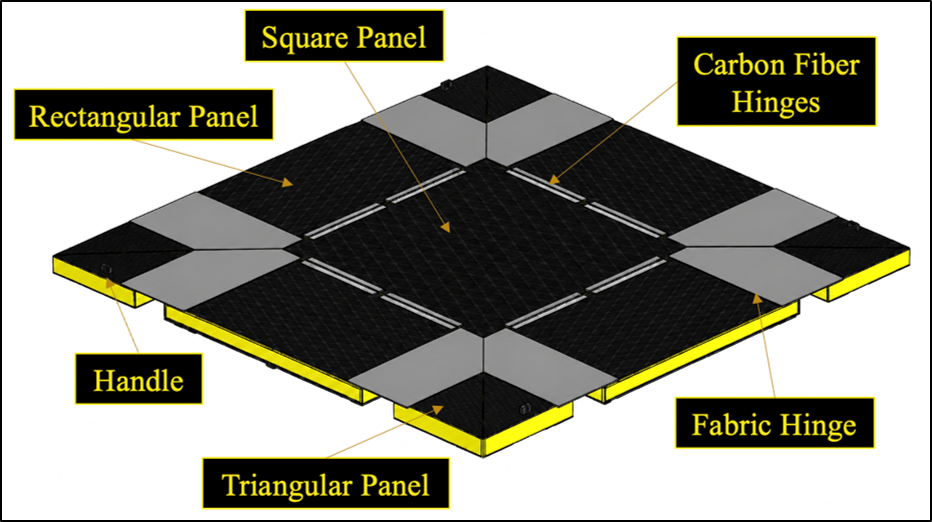
\includegraphics[
        width=1.92in,
        height=1.30in,
        keepaspectratio
    ]{Toro_Cover_topside_Cad}
};
\draw[RuleGray,line width=0.55pt,rounded corners=4pt]
    ($(current page.north west)+(0.43in,-5.04in)$)
    rectangle
    ($(current page.north west)+(2.51in,-6.43in)$);

% Image 2: underside CAD
\node[anchor=center,inner sep=0pt]
at ($(current page.north west)+(3.66in,-5.73in)$)
{
    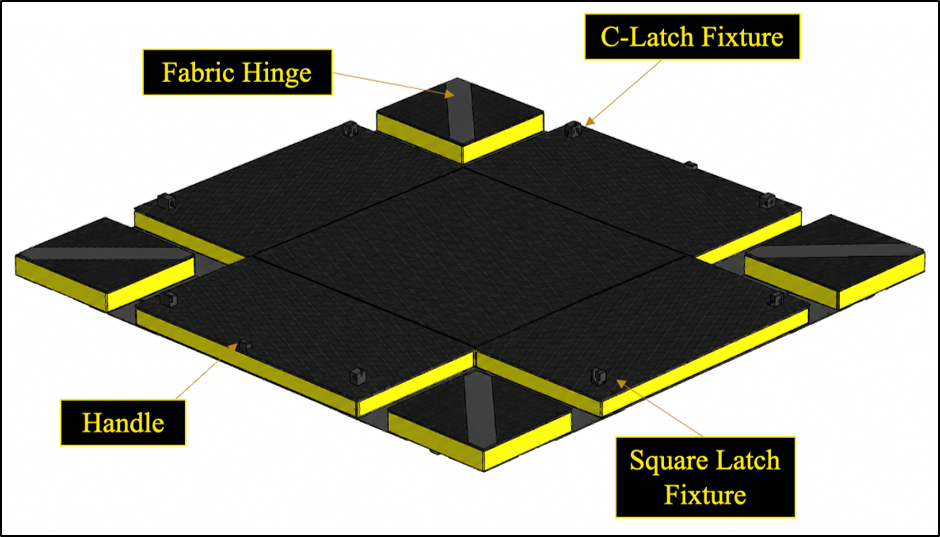
\includegraphics[
        width=1.92in,
        height=1.30in,
        keepaspectratio
    ]{toro_cover_underside_cad}
};
\draw[RuleGray,line width=0.55pt,rounded corners=4pt]
    ($(current page.north west)+(2.62in,-5.04in)$)
    rectangle
    ($(current page.north west)+(4.70in,-6.43in)$);

% Image 3: folded CAD
\node[anchor=center,inner sep=0pt]
at ($(current page.north west)+(5.85in,-5.73in)$)
{
    \includegraphics[
        width=1.92in,
        height=1.30in,
        keepaspectratio
    ]{\detokenize{Toro_Cover_folded Configuration}}
};
\draw[RuleGray,line width=0.55pt,rounded corners=4pt]
    ($(current page.north west)+(4.81in,-5.04in)$)
    rectangle
    ($(current page.north west)+(6.89in,-6.43in)$);

% Image 4: dual-use product concept
\node[anchor=center,inner sep=0pt]
at ($(current page.north west)+(8.04in,-5.73in)$)
{
    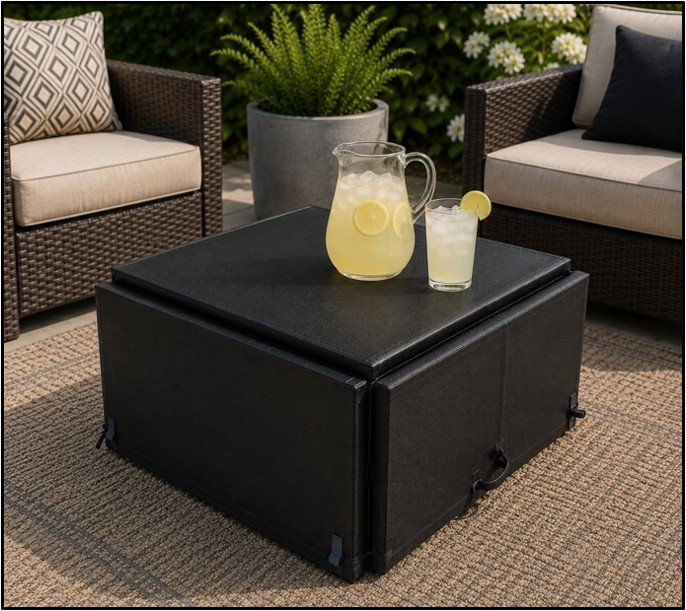
\includegraphics[
        width=1.92in,
        height=1.30in,
        keepaspectratio
    ]{generative_AI_concept_toro_cover_art}
};
\draw[RuleGray,line width=0.55pt,rounded corners=4pt]
    ($(current page.north west)+(7.00in,-5.04in)$)
    rectangle
    ($(current page.north west)+(9.08in,-6.43in)$);

% Image 5: folded foam functional prototype
% The portrait photograph is deliberately clipped to the landscape frame
% so the ottoman fills the card without extending beyond its border.
\begin{scope}
\clip[rounded corners=4pt]
    ($(current page.north west)+(9.19in,-5.04in)$)
    rectangle
    ($(current page.north east)+(-0.43in,-6.43in)$);

% Keep the original image proportions and center it within the existing card.
\node[anchor=center,inner sep=0pt]
at ($(current page.north west)+(9.88in,-5.735in)$)
{
    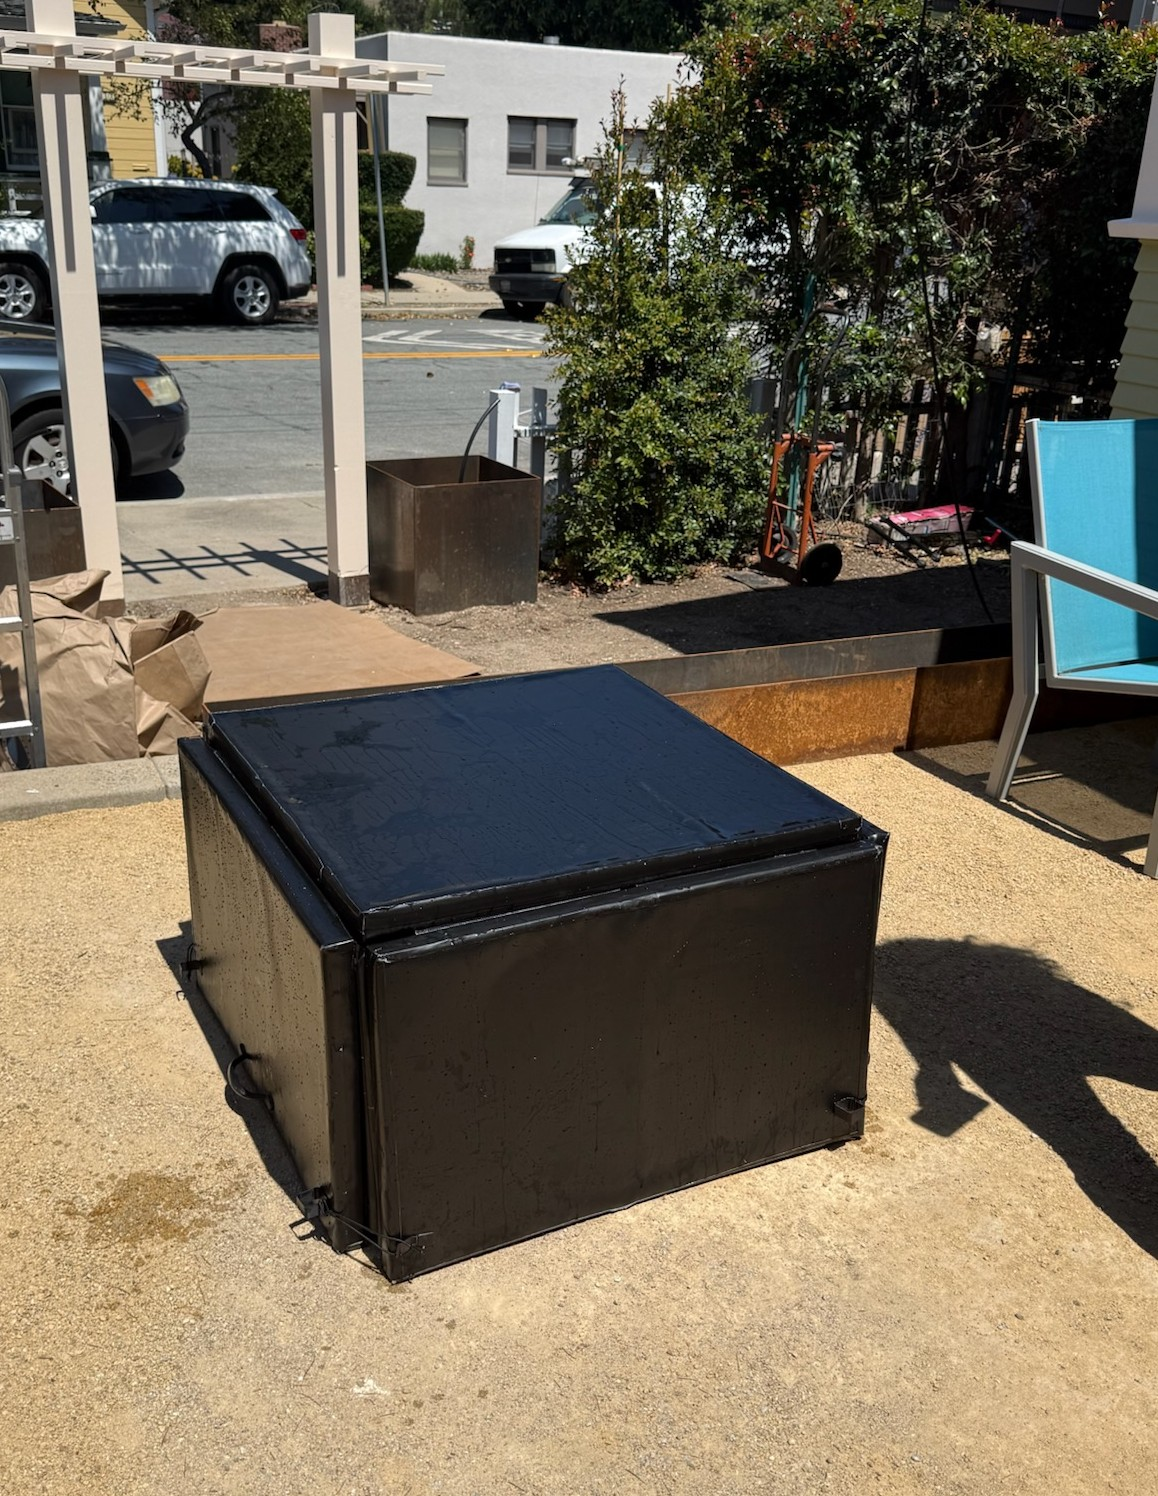
\includegraphics[
        width=1.58in,
        height=1.28in,
        keepaspectratio
    ]{foam_model_folded_backyard_image}
};
\end{scope}

\draw[RuleGray,line width=0.55pt,rounded corners=4pt]
    ($(current page.north west)+(9.19in,-5.04in)$)
    rectangle
    ($(current page.north east)+(-0.43in,-6.43in)$);

% Larger captions
\node[anchor=north,align=center,text width=1.95in,text=Muted,
      font=\sffamily\fontsize{6.8}{7.4}\selectfont]
at ($(current page.north west)+(1.47in,-6.49in)$)
{Topside panel architecture};

\node[anchor=north,align=center,text width=1.95in,text=Muted,
      font=\sffamily\fontsize{6.8}{7.4}\selectfont]
at ($(current page.north west)+(3.66in,-6.49in)$)
{Underside hinge architecture};

\node[anchor=north,align=center,text width=1.95in,text=Muted,
      font=\sffamily\fontsize{6.8}{7.4}\selectfont]
at ($(current page.north west)+(5.85in,-6.49in)$)
{Folded CAD configuration};

\node[anchor=north,align=center,text width=1.95in,text=Muted,
      font=\sffamily\fontsize{6.8}{7.4}\selectfont]
at ($(current page.north west)+(8.04in,-6.49in)$)
{Dual-use product vision};

\node[anchor=north,align=center,text width=1.95in,text=Muted,
      font=\sffamily\fontsize{6.8}{7.4}\selectfont]
at ($(current page.north west)+(9.88in,-6.49in)$)
{Folded foam prototype};

% Page 1 resource bar — centered and non-repeated resources
\fill[Panel,rounded corners=4pt]
    ($(current page.north west)+(0.43in,-7.05in)$)
    rectangle
    ($(current page.north east)+(-0.43in,-7.64in)$);
\draw[RuleGray,line width=0.5pt,rounded corners=4pt]
    ($(current page.north west)+(0.43in,-7.05in)$)
    rectangle
    ($(current page.north east)+(-0.43in,-7.64in)$);

\node[
    anchor=center,
    align=center,
    text=DeepGreen,
    font=\sffamily\bfseries\fontsize{6.9}{7.5}\selectfont
]
at ($(current page.north)+(0,-7.345in)$)
{\href{\ToroDrawingLink}{\faDraftingCompass\ DRAWING PACKAGE}
\hspace{24pt}
\href{\ToroDimensionsLink}{\faImage\ DIMENSION STUDY}
\hspace{24pt}
\href{\ToroProblemLink}{\faFileImage\ PROBLEM STATEMENT}};

% Footer
\node[
    anchor=south west,
    text=white,
    font=\sffamily\bfseries\fontsize{7.1}{7.7}\selectfont
]
at ($(current page.south west)+(0.42in,0.17in)$)
{\hyperlink{composites}{\faArrowLeft\ COMPOSITES}};

\node[
    anchor=south,
    text=white,
    font=\sffamily\fontsize{7.0}{7.6}\selectfont
]
at ($(current page.south)+(0,0.17in)$)
{TORO COVER \hspace{6pt} 1 / 3};

\node[
    anchor=south east,
    text=white,
    font=\sffamily\bfseries\fontsize{7.1}{7.7}\selectfont
]
at ($(current page.south east)+(-0.42in,0.17in)$)
{MANUFACTURING-DRIVEN DESIGN \faArrowRight};

\end{tikzpicture}


% ============================================================
% PAGE 2 — MANUFACTURING-DRIVEN DESIGN
% ============================================================

\clearpage
\thispagestyle{empty}
\hypertarget{toro-manufacturing}{}
\null

\begin{tikzpicture}[remember picture,overlay]

% Background and bars
\fill[white]
    (current page.south west)
    rectangle
    (current page.north east);

\fill[DeepGreen]
    (current page.north west)
    rectangle
    ($(current page.north east)+(0,-0.095in)$);

\fill[PolyGold]
    ($(current page.north west)+(0,-0.095in)$)
    rectangle
    ($(current page.north east)+(0,-0.14in)$);

\fill[DeepGreen]
    (current page.south west)
    rectangle
    ($(current page.south east)+(0,0.36in)$);

\fill[PolyGold]
    ($(current page.south west)+(0,0.36in)$)
    rectangle
    ($(current page.south east)+(0,0.405in)$);

% Header
\node[
    anchor=north west,
    text=PolyGold,
    font=\sffamily\bfseries\fontsize{8.1}{8.7}\selectfont
]
at ($(current page.north west)+(0.42in,-0.39in)$)
{TORO COVER \hspace{5pt}/\hspace{5pt} DESIGN FOR MANUFACTURABILITY};

\node[
    anchor=north west,
    text=DeepGreen,
    font=\bfseries\fontsize{23}{24}\selectfont
]
at ($(current page.north west)+(0.40in,-0.67in)$)
{THE ENVELOPE METHOD};

\node[
    anchor=north west,
    text=Muted,
    font=\sffamily\fontsize{8.7}{9.6}\selectfont
]
at ($(current page.north west)+(0.42in,-1.12in)$)
{A one-layup process developed for unusually thick insulated composite sandwich panels};

\fill[PolyGold]
    ($(current page.north west)+(0.42in,-1.36in)$)
    rectangle
    ($(current page.north west)+(5.30in,-1.315in)$);

% Process explanation
\fill[SoftGold,rounded corners=5pt]
    ($(current page.north west)+(0.42in,-1.61in)$)
    rectangle
    ($(current page.north east)+(-0.42in,-2.90in)$);

\fill[PolyGold]
    ($(current page.north west)+(0.42in,-1.61in)$)
    rectangle
    ($(current page.north west)+(0.52in,-2.90in)$);

\node[
    anchor=north west,
    text=DeepGreen,
    font=\sffamily\bfseries\fontsize{7.9}{8.6}\selectfont
]
at ($(current page.north west)+(0.67in,-1.76in)$)
{PROCESS INNOVATION};

\node[
    anchor=north west,
    align=left,
    text width=9.55in,
    text=Ink,
    font=\fontsize{7.35}{8.75}\selectfont
]
at ($(current page.north west)+(0.67in,-2.02in)$)
{
Weight reduction and insulation were both essential, leading to the selection of an
XPS foam core. Because XPS could not tolerate composite heat-cure temperatures, prepreg
processing was not practical and the panels had to be manufactured by wet layup with a
room-temperature cure. To simplify this process, I waterjet-cut XPS perimeter strips from
excess foam and placed them around each core inside the vacuum enclosure. Under vacuum,
the top and bottom carbon skins met along the panel sides and compressed against this
border, eliminating a separate edge-banding layup and reducing corner pleating.
};

% Workflow title
\node[
    anchor=north west,
    text=DeepGreen,
    font=\sffamily\bfseries\fontsize{8.0}{8.7}\selectfont
]
at ($(current page.north west)+(0.43in,-3.06in)$)
{MANUFACTURING WORKFLOW};

% Row 1 image 1
\node[anchor=center,inner sep=0pt]
at ($(current page.north west)+(2.07in,-4.105in)$)
{
    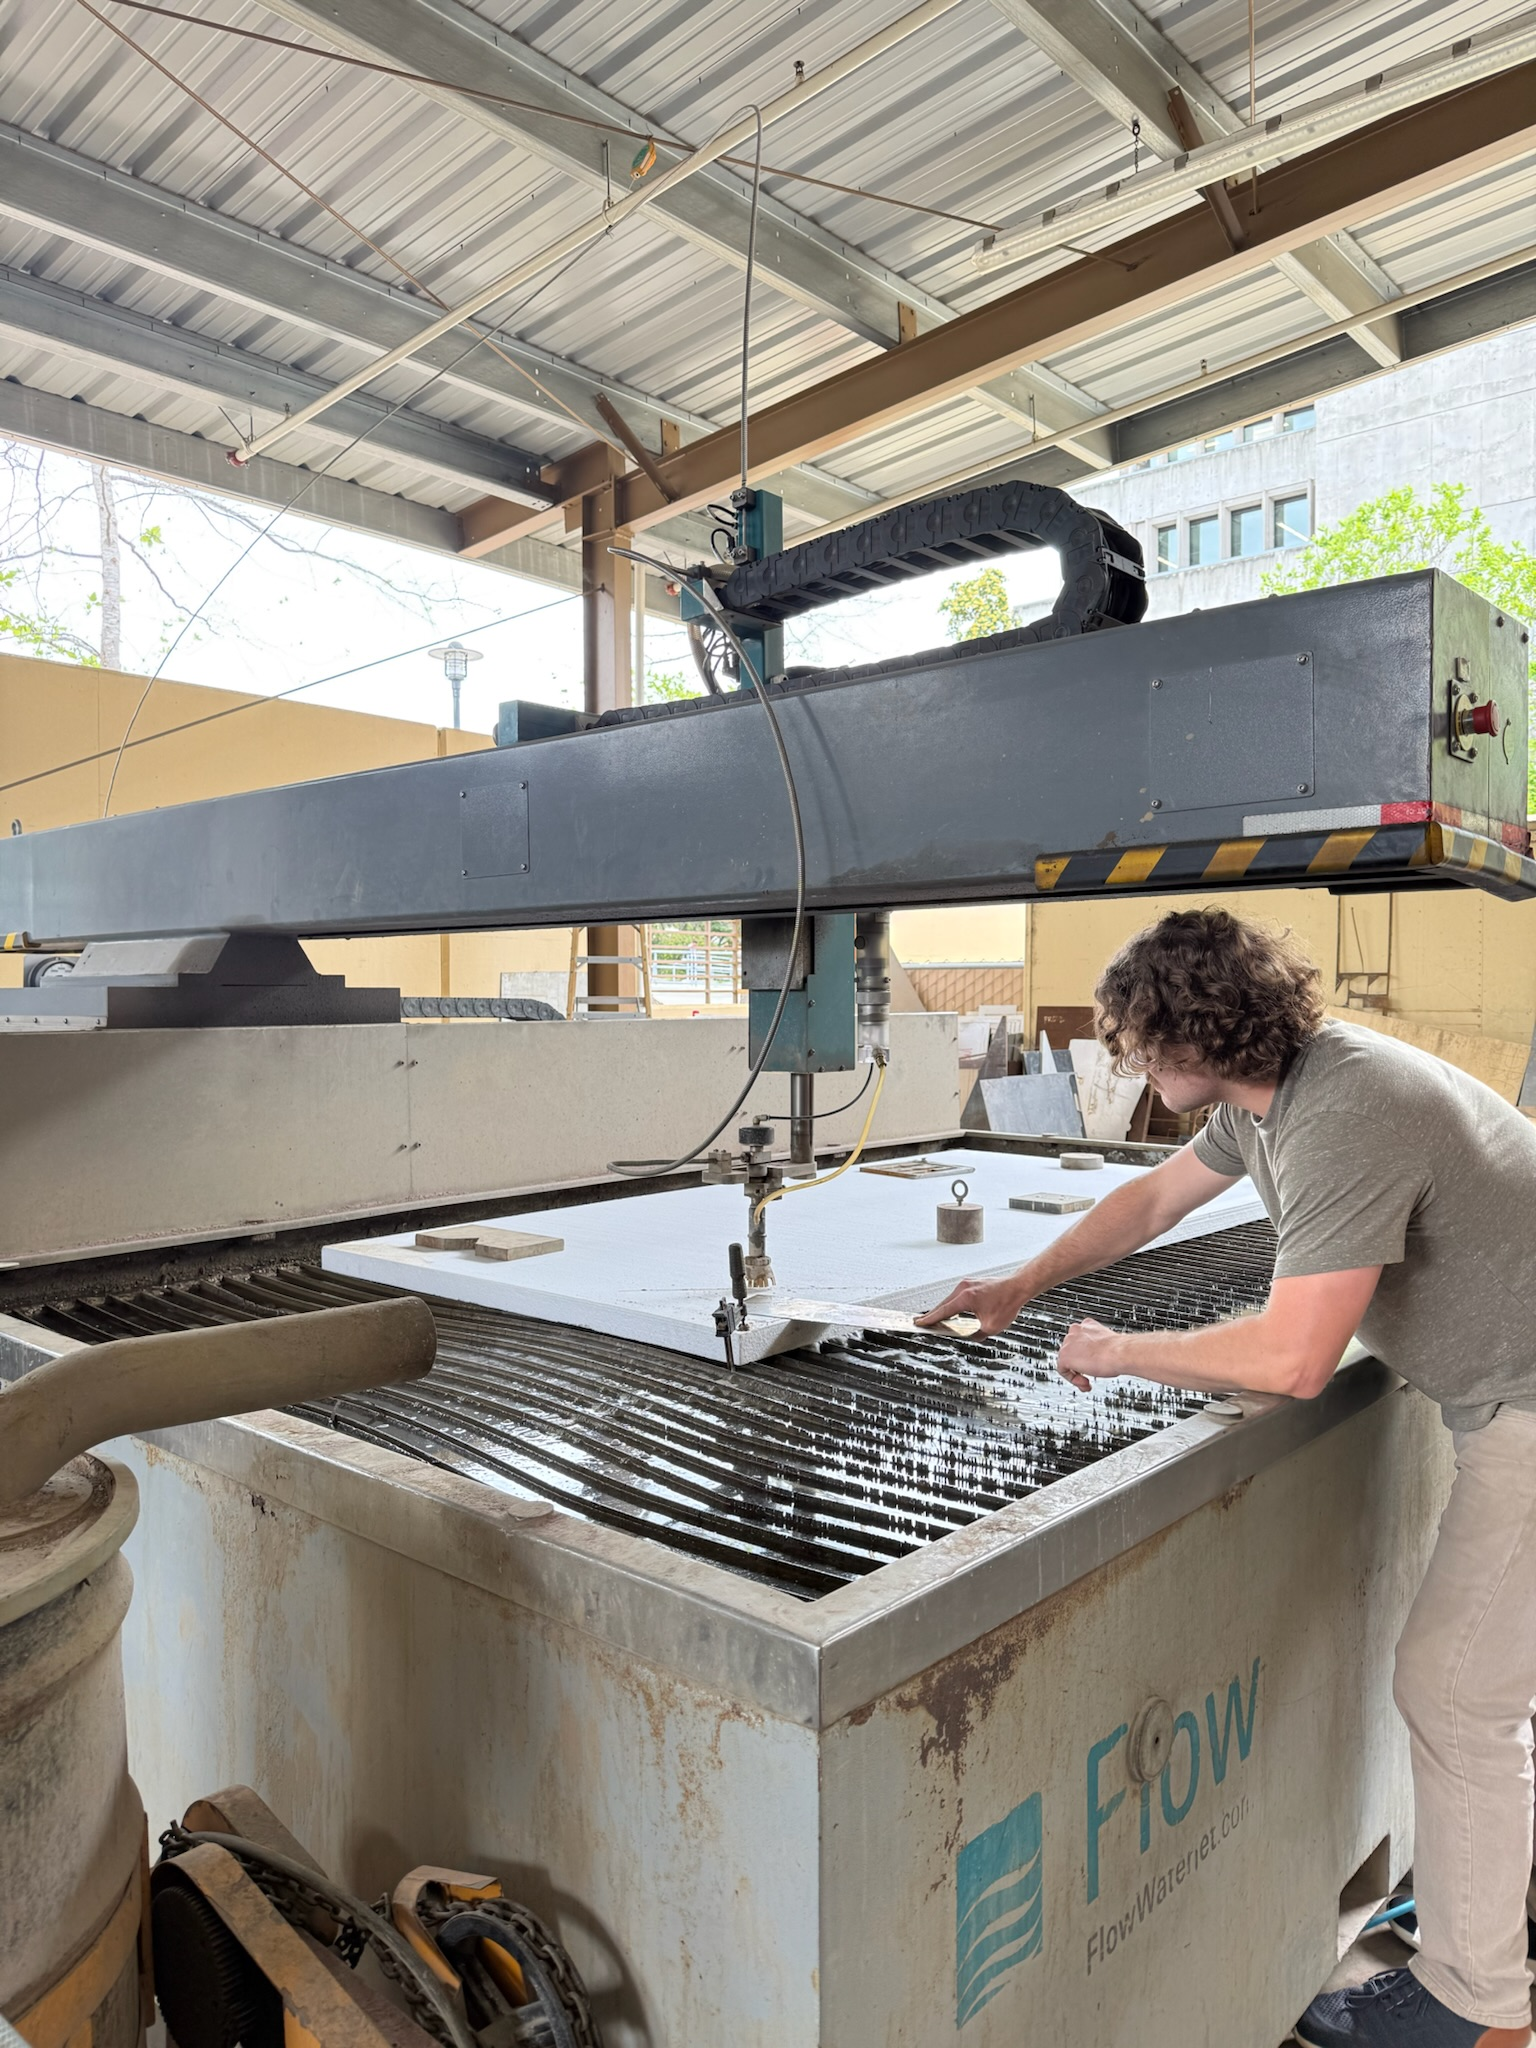
\includegraphics[
        width=3.10in,
        height=1.40in,
        keepaspectratio
    ]{waterjet_foam}
};
\draw[RuleGray,line width=0.55pt,rounded corners=4pt]
    ($(current page.north west)+(0.43in,-3.36in)$)
    rectangle
    ($(current page.north west)+(3.71in,-4.85in)$);

% Row 1 image 2
\node[anchor=center,inner sep=0pt]
at ($(current page.north west)+(5.50in,-4.105in)$)
{
    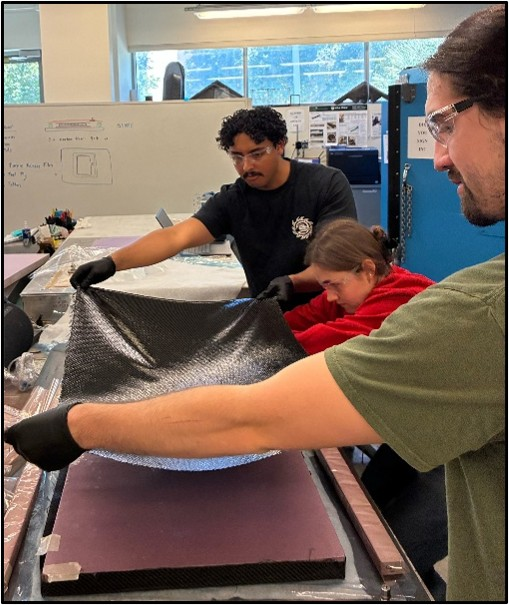
\includegraphics[
        width=3.10in,
        height=1.40in,
        keepaspectratio
    ]{group_layup}
};
\draw[RuleGray,line width=0.55pt,rounded corners=4pt]
    ($(current page.north west)+(3.86in,-3.36in)$)
    rectangle
    ($(current page.north west)+(7.14in,-4.85in)$);

% Row 1 image 3
\node[anchor=center,inner sep=0pt]
at ($(current page.north west)+(8.935in,-4.105in)$)
{
    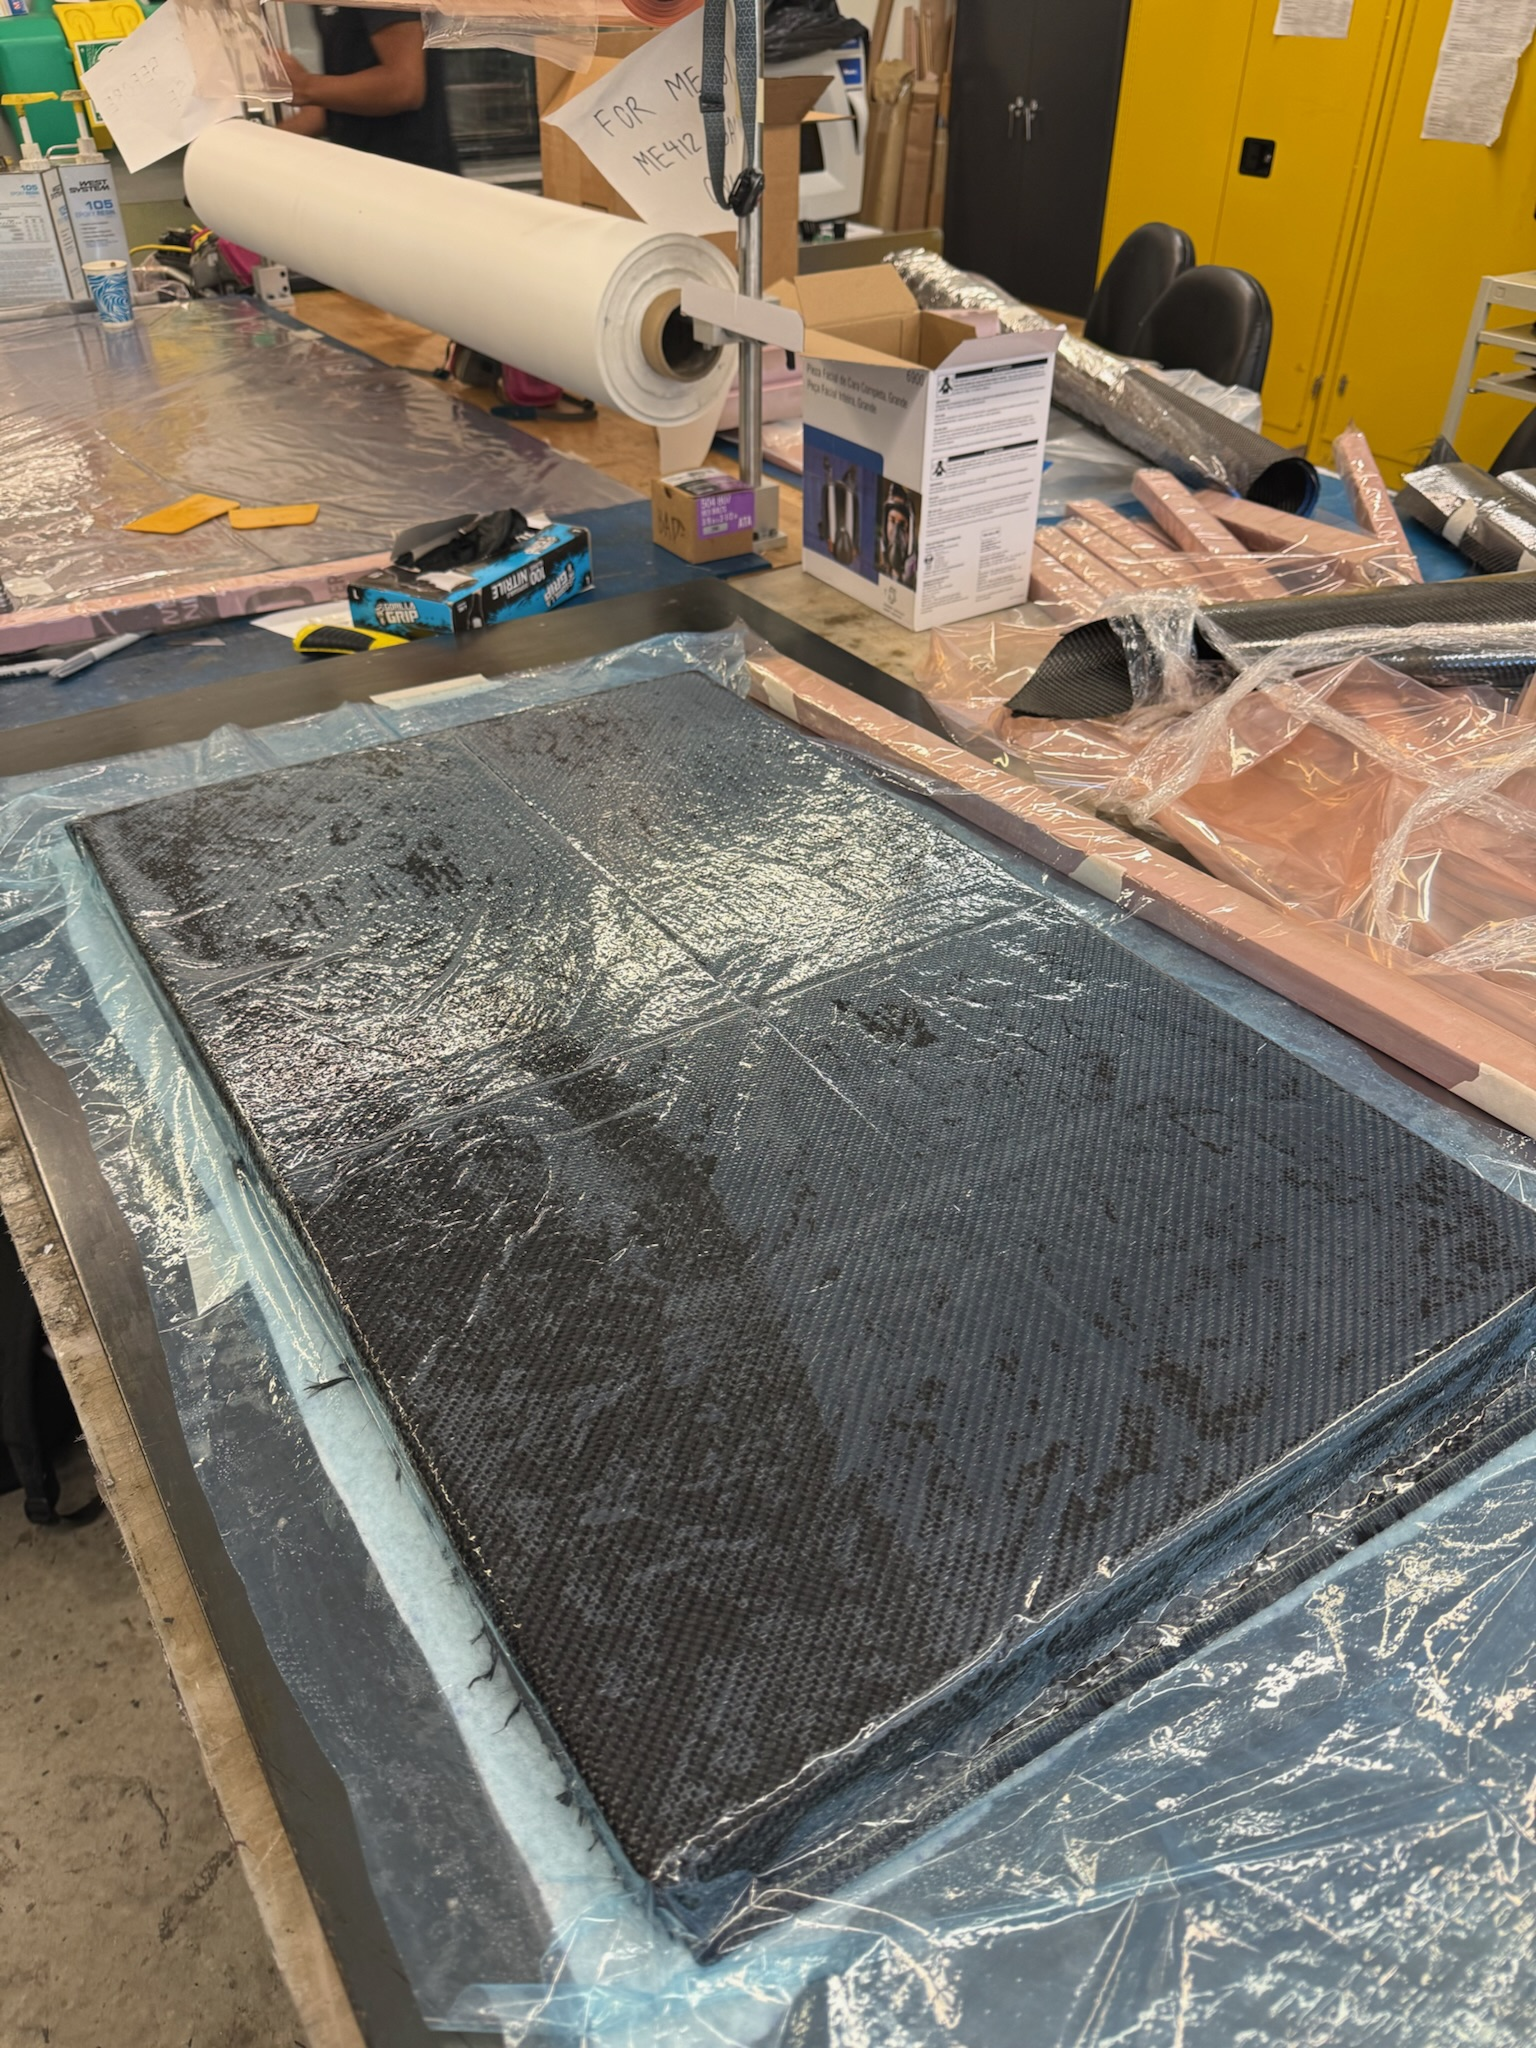
\includegraphics[
        width=3.10in,
        height=1.40in,
        keepaspectratio
    ]{blue_perforrated_film_layup}
};
\draw[RuleGray,line width=0.55pt,rounded corners=4pt]
    ($(current page.north west)+(7.29in,-3.36in)$)
    rectangle
    ($(current page.north east)+(-0.42in,-4.85in)$);

% Row 1 captions
\node[anchor=north,text=Muted,font=\sffamily\fontsize{6.7}{7.3}\selectfont]
at ($(current page.north west)+(2.07in,-4.90in)$)
{1. Waterjet-cut core and perimeter geometry};

\node[anchor=north,text=Muted,font=\sffamily\fontsize{6.7}{7.3}\selectfont]
at ($(current page.north west)+(5.50in,-4.90in)$)
{2. Team wet layup under my process guidance};

\node[anchor=north,text=Muted,font=\sffamily\fontsize{6.7}{7.3}\selectfont]
at ($(current page.north west)+(8.935in,-4.90in)$)
{3. Perforated film, breather, and vacuum enclosure};

% Row 2 image 1
\node[anchor=center,inner sep=0pt]
at ($(current page.north west)+(2.07in,-5.875in)$)
{
    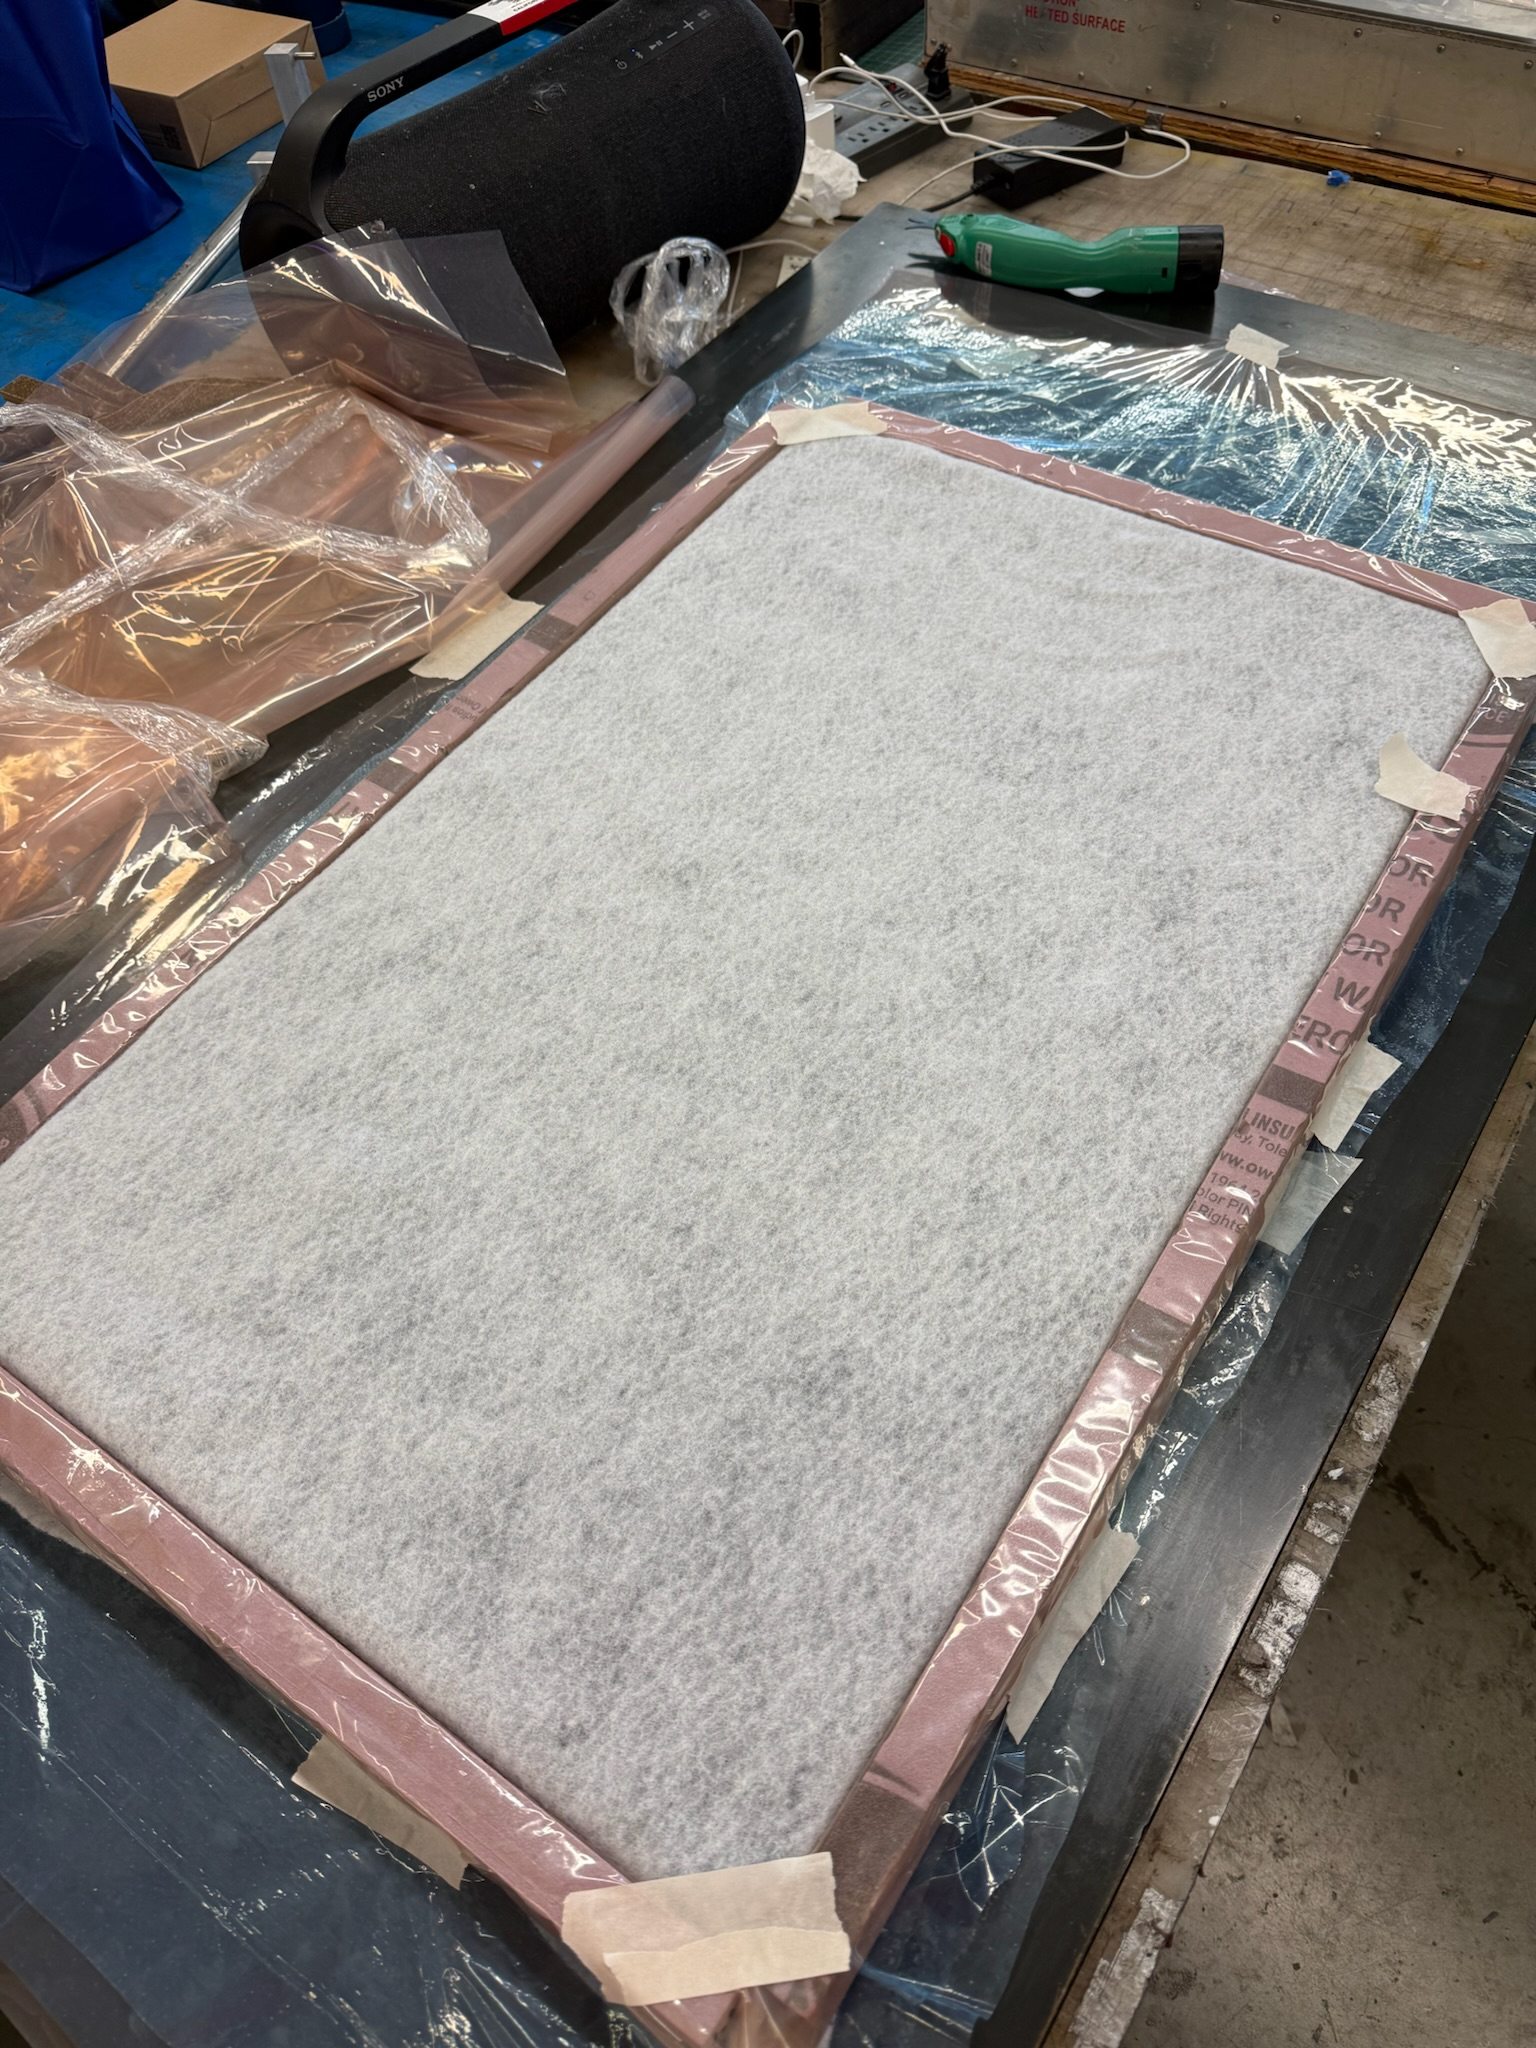
\includegraphics[
        width=3.10in,
        height=1.40in,
        keepaspectratio
    ]{completed_layup}
};
\draw[RuleGray,line width=0.55pt,rounded corners=4pt]
    ($(current page.north west)+(0.43in,-5.13in)$)
    rectangle
    ($(current page.north west)+(3.71in,-6.62in)$);

% Row 2 image 2 — oven chamber used only as a reliable vacuum enclosure; no heat applied
\node[anchor=center,inner sep=0pt]
at ($(current page.north west)+(5.50in,-5.875in)$)
{
    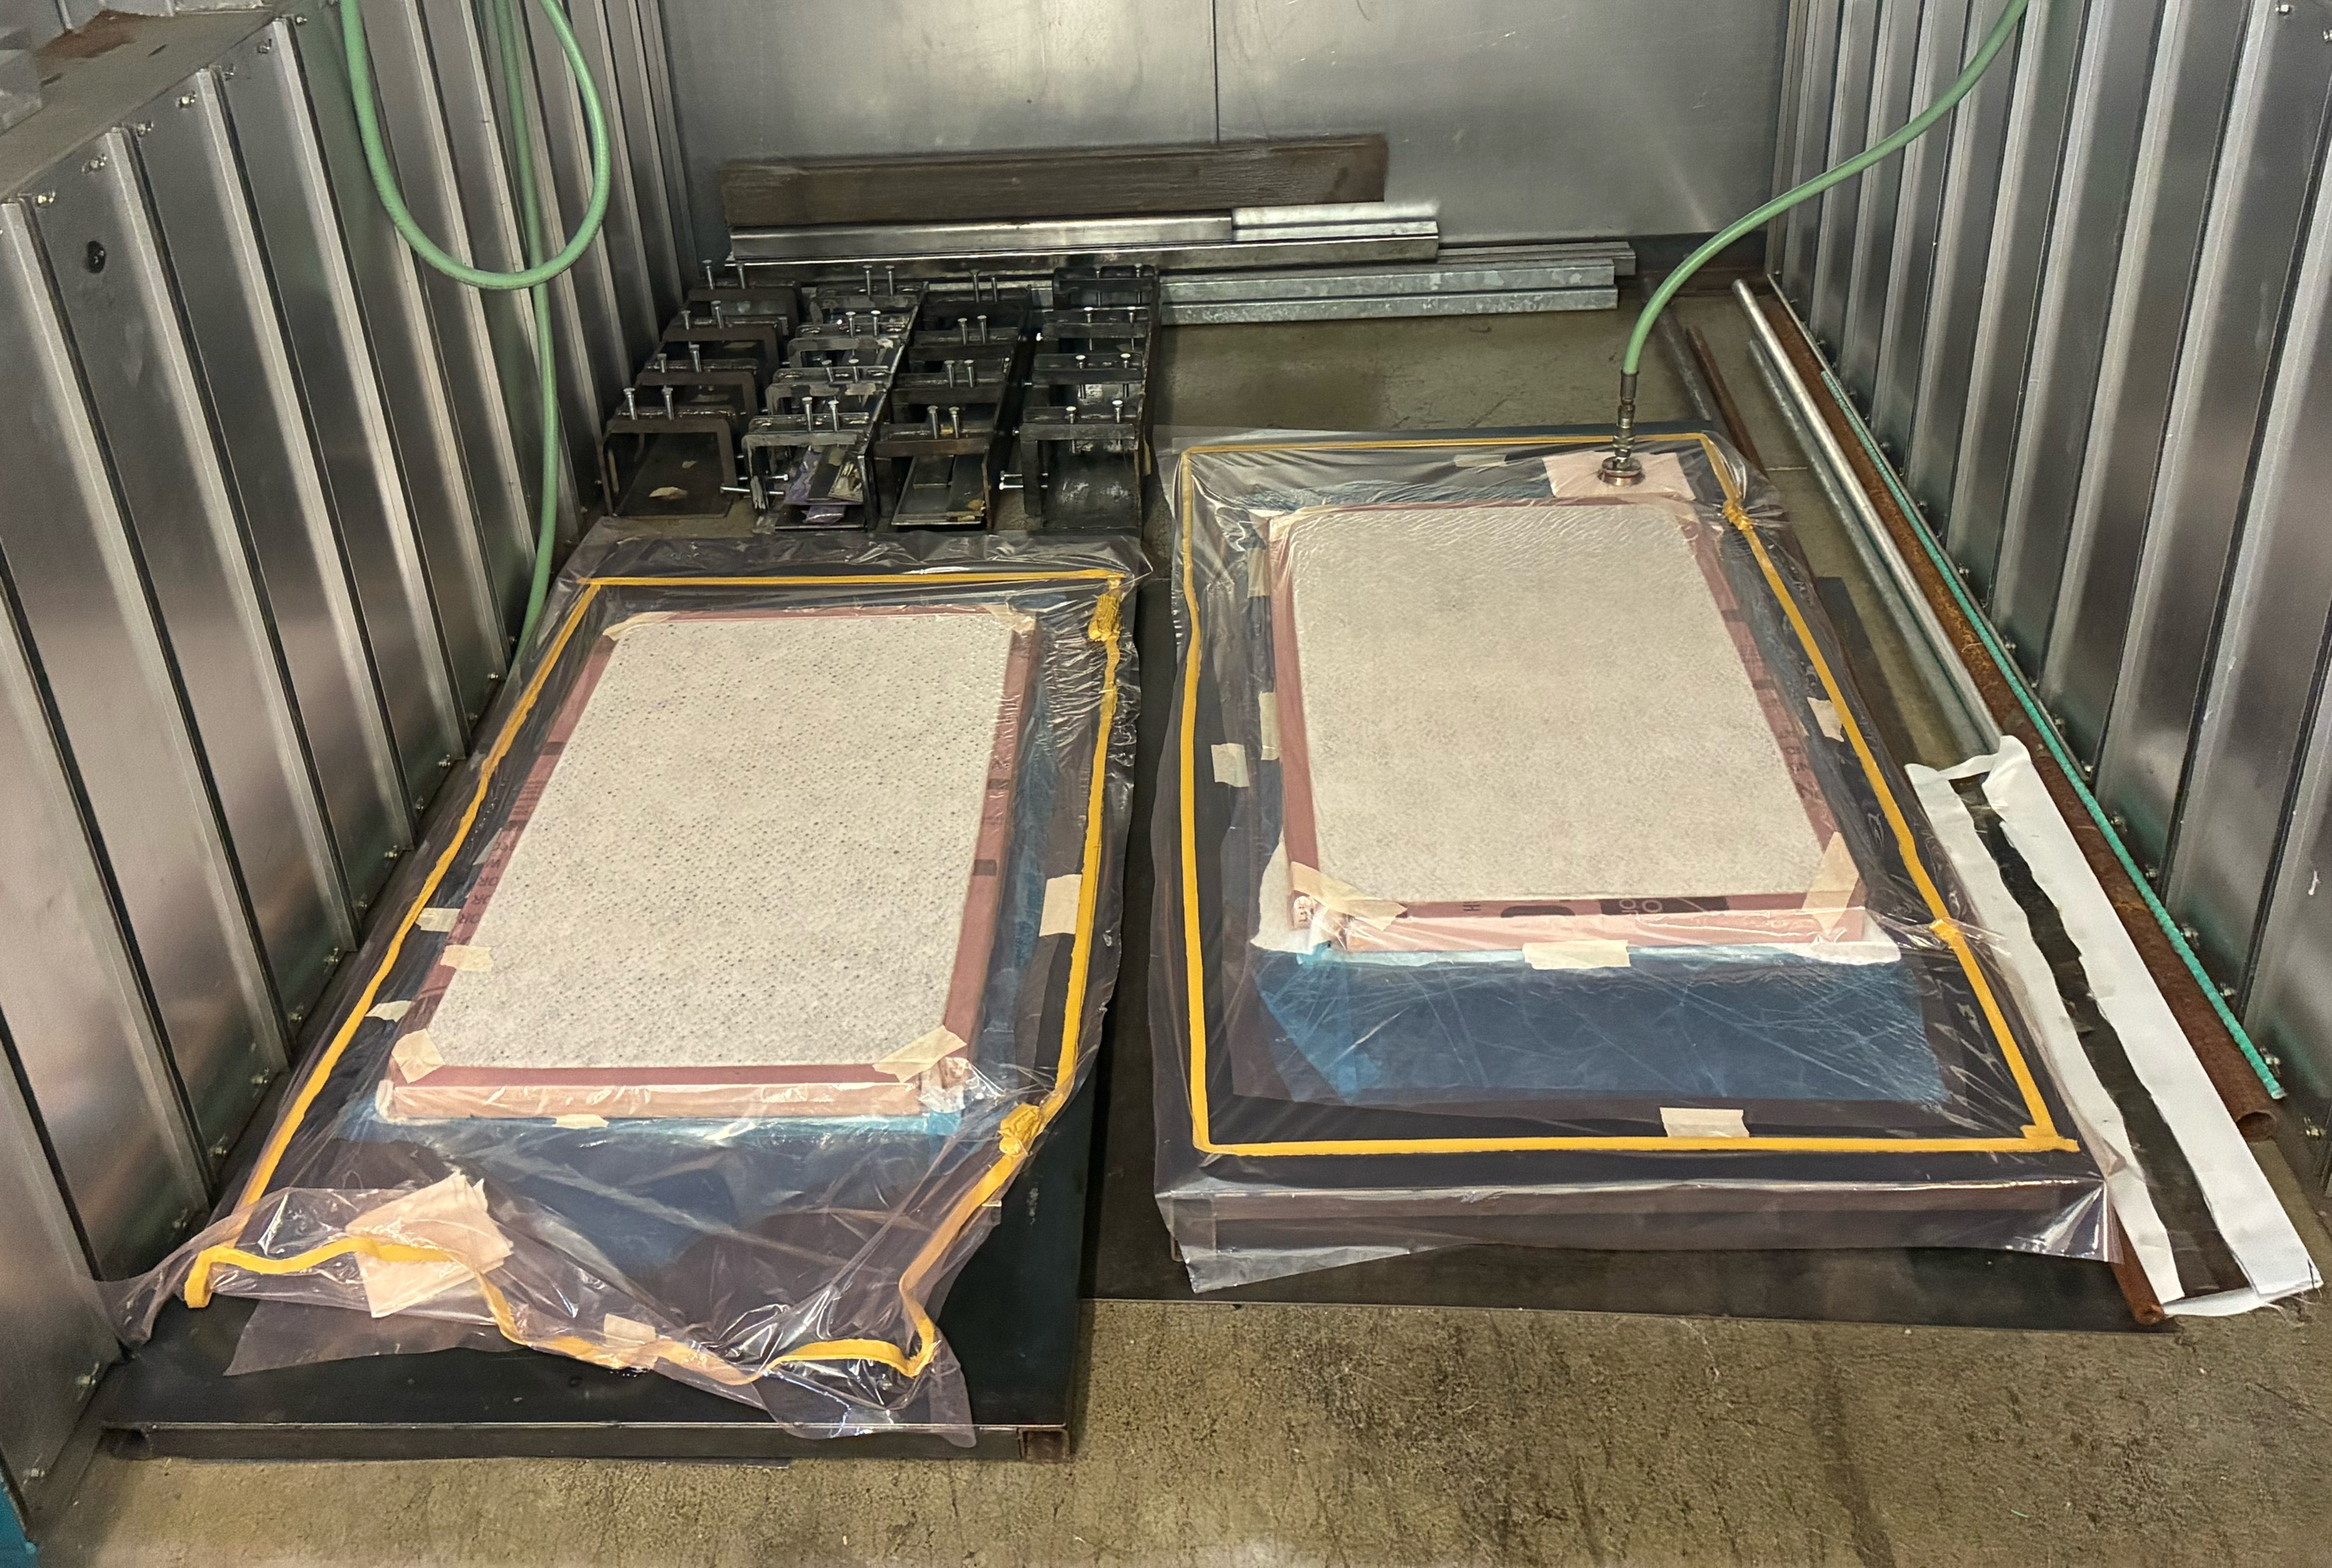
\includegraphics[
        width=3.10in,
        height=1.40in,
        keepaspectratio
    ]{layups_in_composite_oven_under_vacuumPressure}
};
\draw[RuleGray,line width=0.55pt,rounded corners=4pt]
    ($(current page.north west)+(3.86in,-5.13in)$)
    rectangle
    ($(current page.north west)+(7.14in,-6.62in)$);

% Row 2 image 3
\node[anchor=center,inner sep=0pt]
at ($(current page.north west)+(8.935in,-5.875in)$)
{
    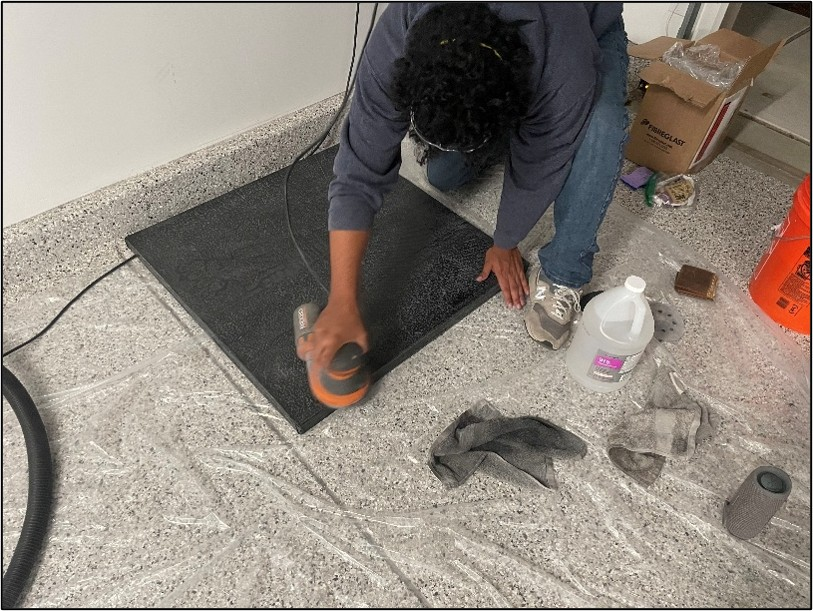
\includegraphics[
        width=3.10in,
        height=1.40in,
        keepaspectratio
    ]{garage_sanding}
};
\draw[RuleGray,line width=0.55pt,rounded corners=4pt]
    ($(current page.north west)+(7.29in,-5.13in)$)
    rectangle
    ($(current page.north east)+(-0.42in,-6.62in)$);

% Row 2 captions
\node[anchor=north,text=Muted,font=\sffamily\fontsize{6.7}{7.3}\selectfont]
at ($(current page.north west)+(2.07in,-6.67in)$)
{4. Fully saturated carbon skin and foam sandwich};

\node[anchor=north,text=Muted,font=\sffamily\fontsize{6.7}{7.3}\selectfont]
at ($(current page.north west)+(5.50in,-6.67in)$)
{5. Room-temperature cure under continuous vacuum};

\node[anchor=north,text=Muted,font=\sffamily\fontsize{6.7}{7.3}\selectfont]
at ($(current page.north west)+(8.935in,-6.67in)$)
{6. Post-processing and surface preparation};

% Bottom callouts
\fill[Panel,rounded corners=4pt]
    ($(current page.north west)+(0.43in,-6.95in)$)
    rectangle
    ($(current page.north west)+(5.48in,-7.60in)$);

\draw[RuleGray,line width=0.55pt,rounded corners=4pt]
    ($(current page.north west)+(0.43in,-6.95in)$)
    rectangle
    ($(current page.north west)+(5.48in,-7.60in)$);

\node[
    anchor=north west,
    text=DeepGreen,
    font=\sffamily\bfseries\fontsize{7.0}{7.6}\selectfont
]
at ($(current page.north west)+(0.63in,-7.08in)$)
{FROM THREE LAYUPS TO ONE};

\node[
    anchor=north west,
    align=left,
    text width=4.56in,
    text=Ink,
    font=\fontsize{6.45}{7.45}\selectfont
]
at ($(current page.north west)+(0.63in,-7.29in)$)
{
The Envelope Method reduced labor, cure cycles, handling,
alignment risk, and time spent forming numerous vacuum-bag
pleats around the 1.5-inch-thick XPS panels.
};

\fill[Panel,rounded corners=4pt]
    ($(current page.north west)+(5.68in,-6.95in)$)
    rectangle
    ($(current page.north east)+(-0.42in,-7.60in)$);

\draw[RuleGray,line width=0.55pt,rounded corners=4pt]
    ($(current page.north west)+(5.68in,-6.95in)$)
    rectangle
    ($(current page.north east)+(-0.42in,-7.60in)$);

\node[
    anchor=north west,
    text=DeepGreen,
    font=\sffamily\bfseries\fontsize{7.0}{7.6}\selectfont
]
at ($(current page.north west)+(5.88in,-7.08in)$)
{WHY SURFACE-BONDED HARDWARE};

\node[
    anchor=north west,
    align=left,
    text width=4.55in,
    text=Ink,
    font=\fontsize{6.45}{7.45}\selectfont
]
at ($(current page.north west)+(5.88in,-7.29in)$)
{
Adhesively bonded hinges and fixtures preserved the clean
composite exterior and avoided drilled inserts, foam-core
crushing, added stress concentrations, and new leak paths.
};


% Footer
\node[
    anchor=south west,
    text=white,
    font=\sffamily\bfseries\fontsize{7.1}{7.7}\selectfont
]
at ($(current page.south west)+(0.42in,0.17in)$)
{\faArrowLeft\ PRODUCT ARCHITECTURE};

\node[
    anchor=south,
    text=white,
    font=\sffamily\fontsize{7.0}{7.6}\selectfont
]
at ($(current page.south)+(0,0.17in)$)
{TORO COVER \hspace{6pt} 2 / 3};

\node[
    anchor=south east,
    text=white,
    font=\sffamily\bfseries\fontsize{7.1}{7.7}\selectfont
]
at ($(current page.south east)+(-0.42in,0.17in)$)
{VALIDATION \& TAKEAWAYS \faArrowRight};

\end{tikzpicture}


% ============================================================
% PAGE 3 — FINISHING, VALIDATION, AND TAKEAWAYS
% ============================================================

\clearpage
\thispagestyle{empty}
\hypertarget{toro-results}{}
\null

\begin{tikzpicture}[remember picture,overlay]

% Background and bars
\fill[white]
    (current page.south west)
    rectangle
    (current page.north east);

\fill[DeepGreen]
    (current page.north west)
    rectangle
    ($(current page.north east)+(0,-0.095in)$);

\fill[PolyGold]
    ($(current page.north west)+(0,-0.095in)$)
    rectangle
    ($(current page.north east)+(0,-0.14in)$);

\fill[DeepGreen]
    (current page.south west)
    rectangle
    ($(current page.south east)+(0,0.36in)$);

\fill[PolyGold]
    ($(current page.south west)+(0,0.36in)$)
    rectangle
    ($(current page.south east)+(0,0.405in)$);

% Header
\node[
    anchor=north west,
    text=PolyGold,
    font=\sffamily\bfseries\fontsize{8.1}{8.7}\selectfont
]
at ($(current page.north west)+(0.42in,-0.39in)$)
{TORO COVER \hspace{5pt}/\hspace{5pt} VALIDATION AND ENGINEERING TAKEAWAYS};

\node[
    anchor=north west,
    text=DeepGreen,
    font=\bfseries\fontsize{22.5}{23.5}\selectfont
]
at ($(current page.north west)+(0.40in,-0.67in)$)
{FROM PROTOTYPE TO PRODUCT PATHWAY};

\node[
    anchor=north west,
    text=Muted,
    font=\sffamily\fontsize{8.7}{9.6}\selectfont
]
at ($(current page.north west)+(0.42in,-1.12in)$)
{Environmental protection, usability testing, scope decisions, and lessons from technical leadership};

\fill[PolyGold]
    ($(current page.north west)+(0.42in,-1.36in)$)
    rectangle
    ($(current page.north west)+(5.8in,-1.315in)$);

% Finishing title
\node[
    anchor=north west,
    text=DeepGreen,
    font=\sffamily\bfseries\fontsize{8.0}{8.7}\selectfont
]
at ($(current page.north west)+(0.43in,-1.62in)$)
{OUTDOOR FINISHING AND ENVIRONMENTAL PROTECTION};

% Image 1
\node[anchor=center,inner sep=0pt]
at ($(current page.north west)+(1.705in,-2.655in)$)
{
    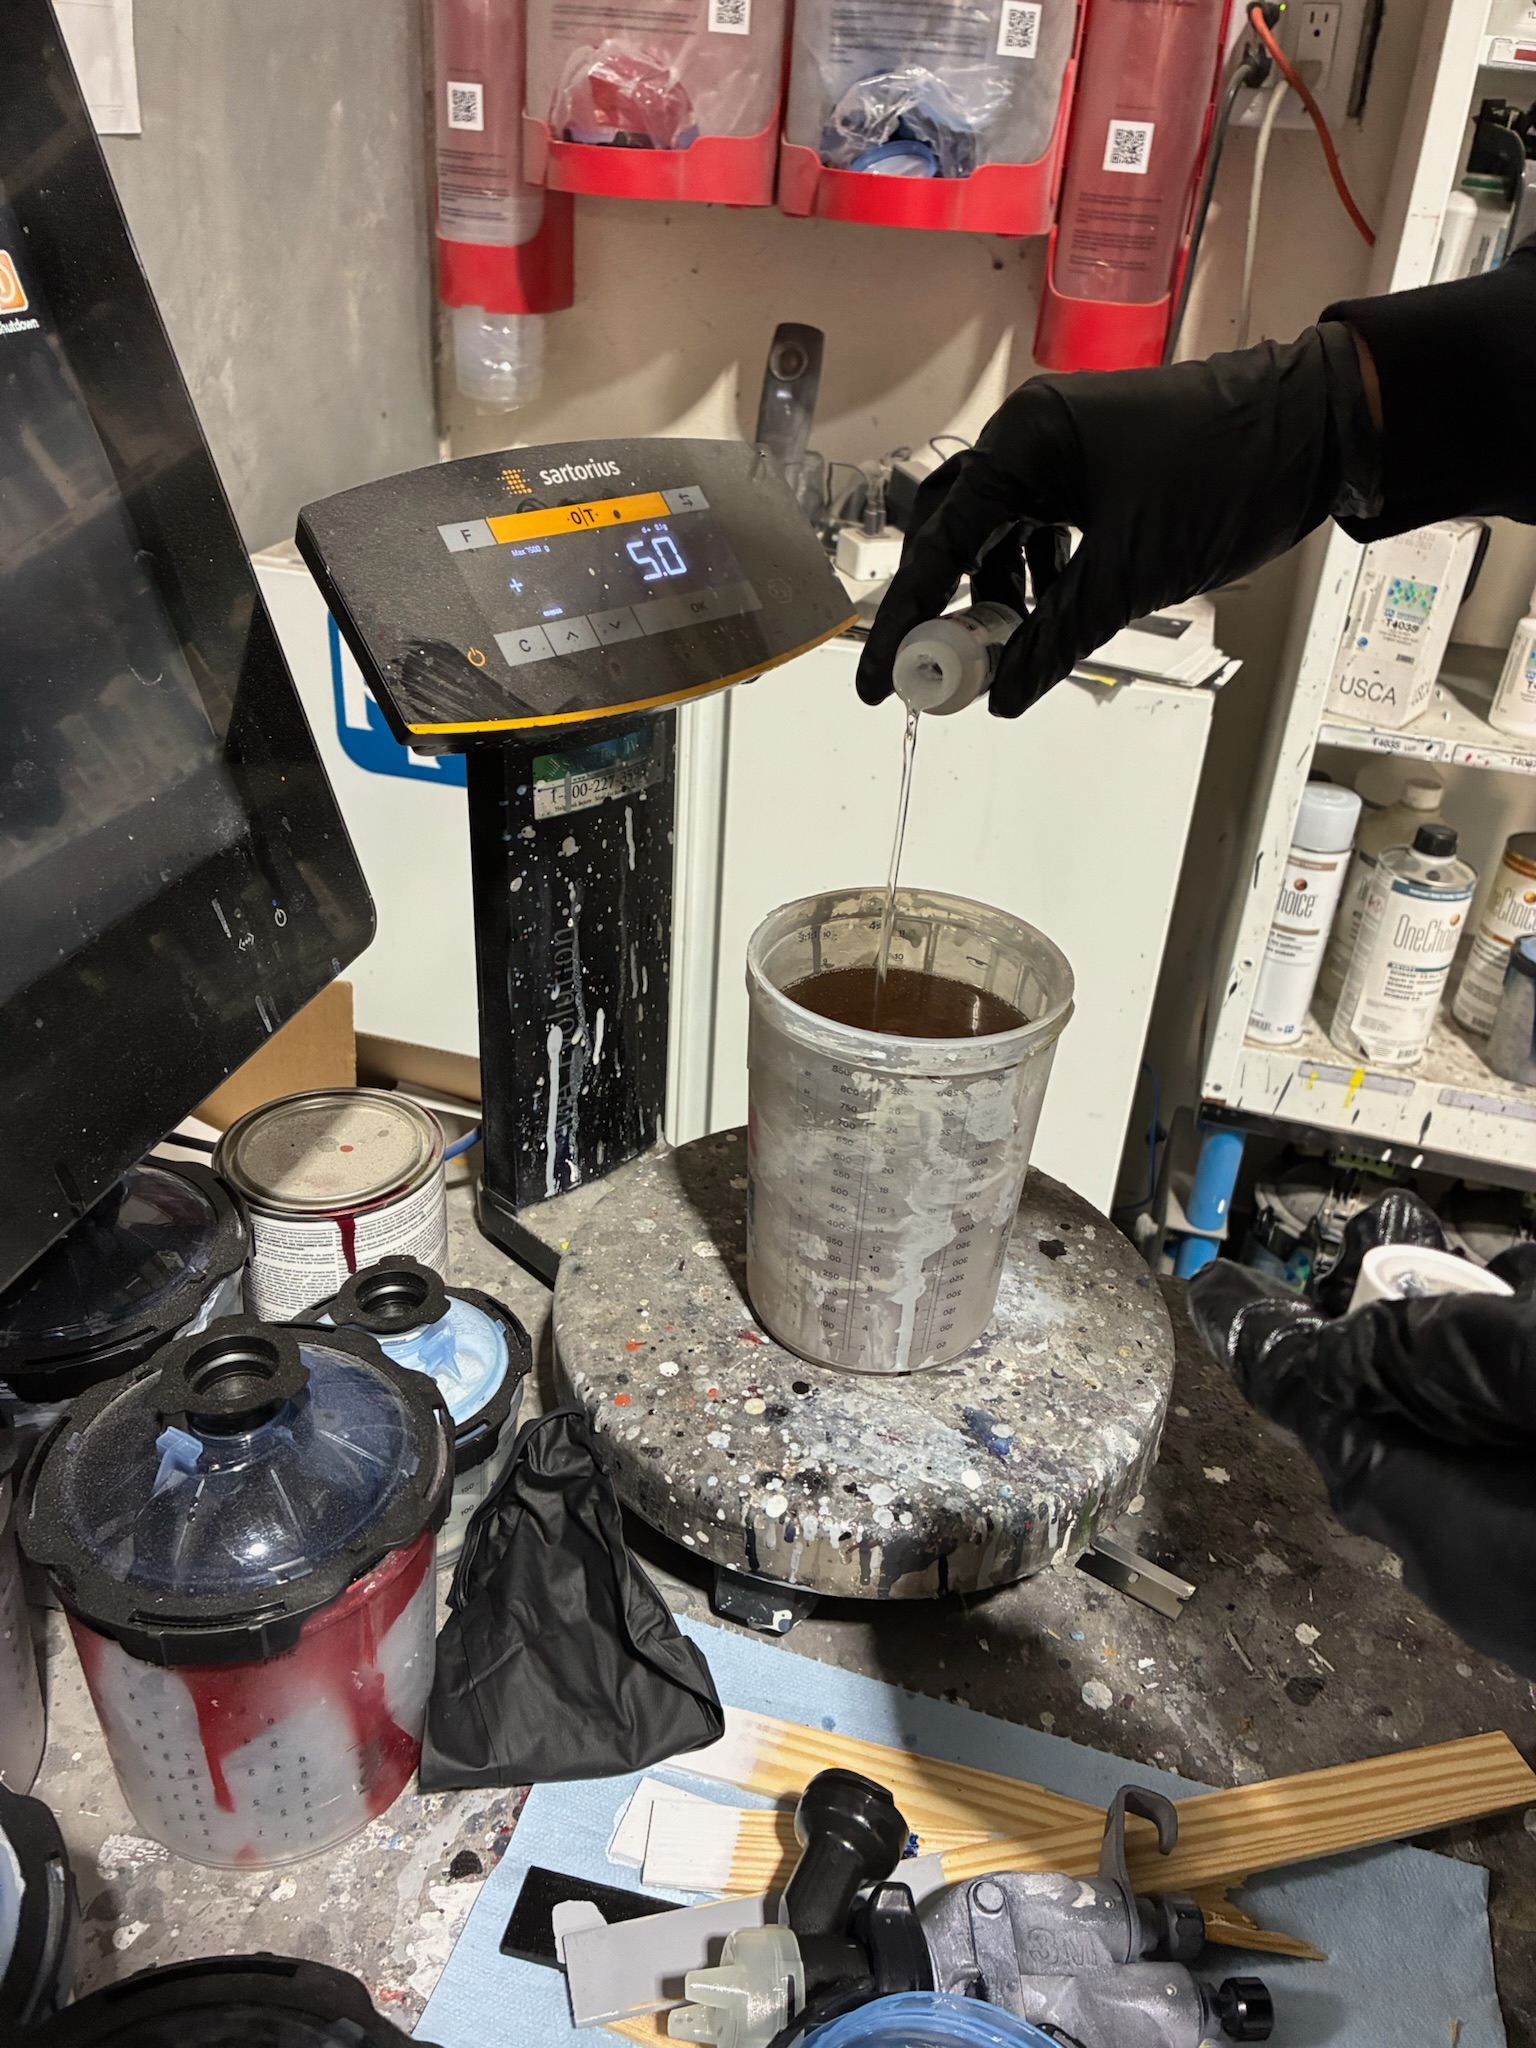
\includegraphics[
        width=2.35in,
        height=1.40in,
        keepaspectratio
    ]{spray_topcoat_prep}
};
\draw[RuleGray,line width=0.55pt,rounded corners=4pt]
    ($(current page.north west)+(0.43in,-1.91in)$)
    rectangle
    ($(current page.north west)+(2.98in,-3.40in)$);

% Image 2
\node[anchor=center,inner sep=0pt]
at ($(current page.north west)+(4.375in,-2.655in)$)
{
    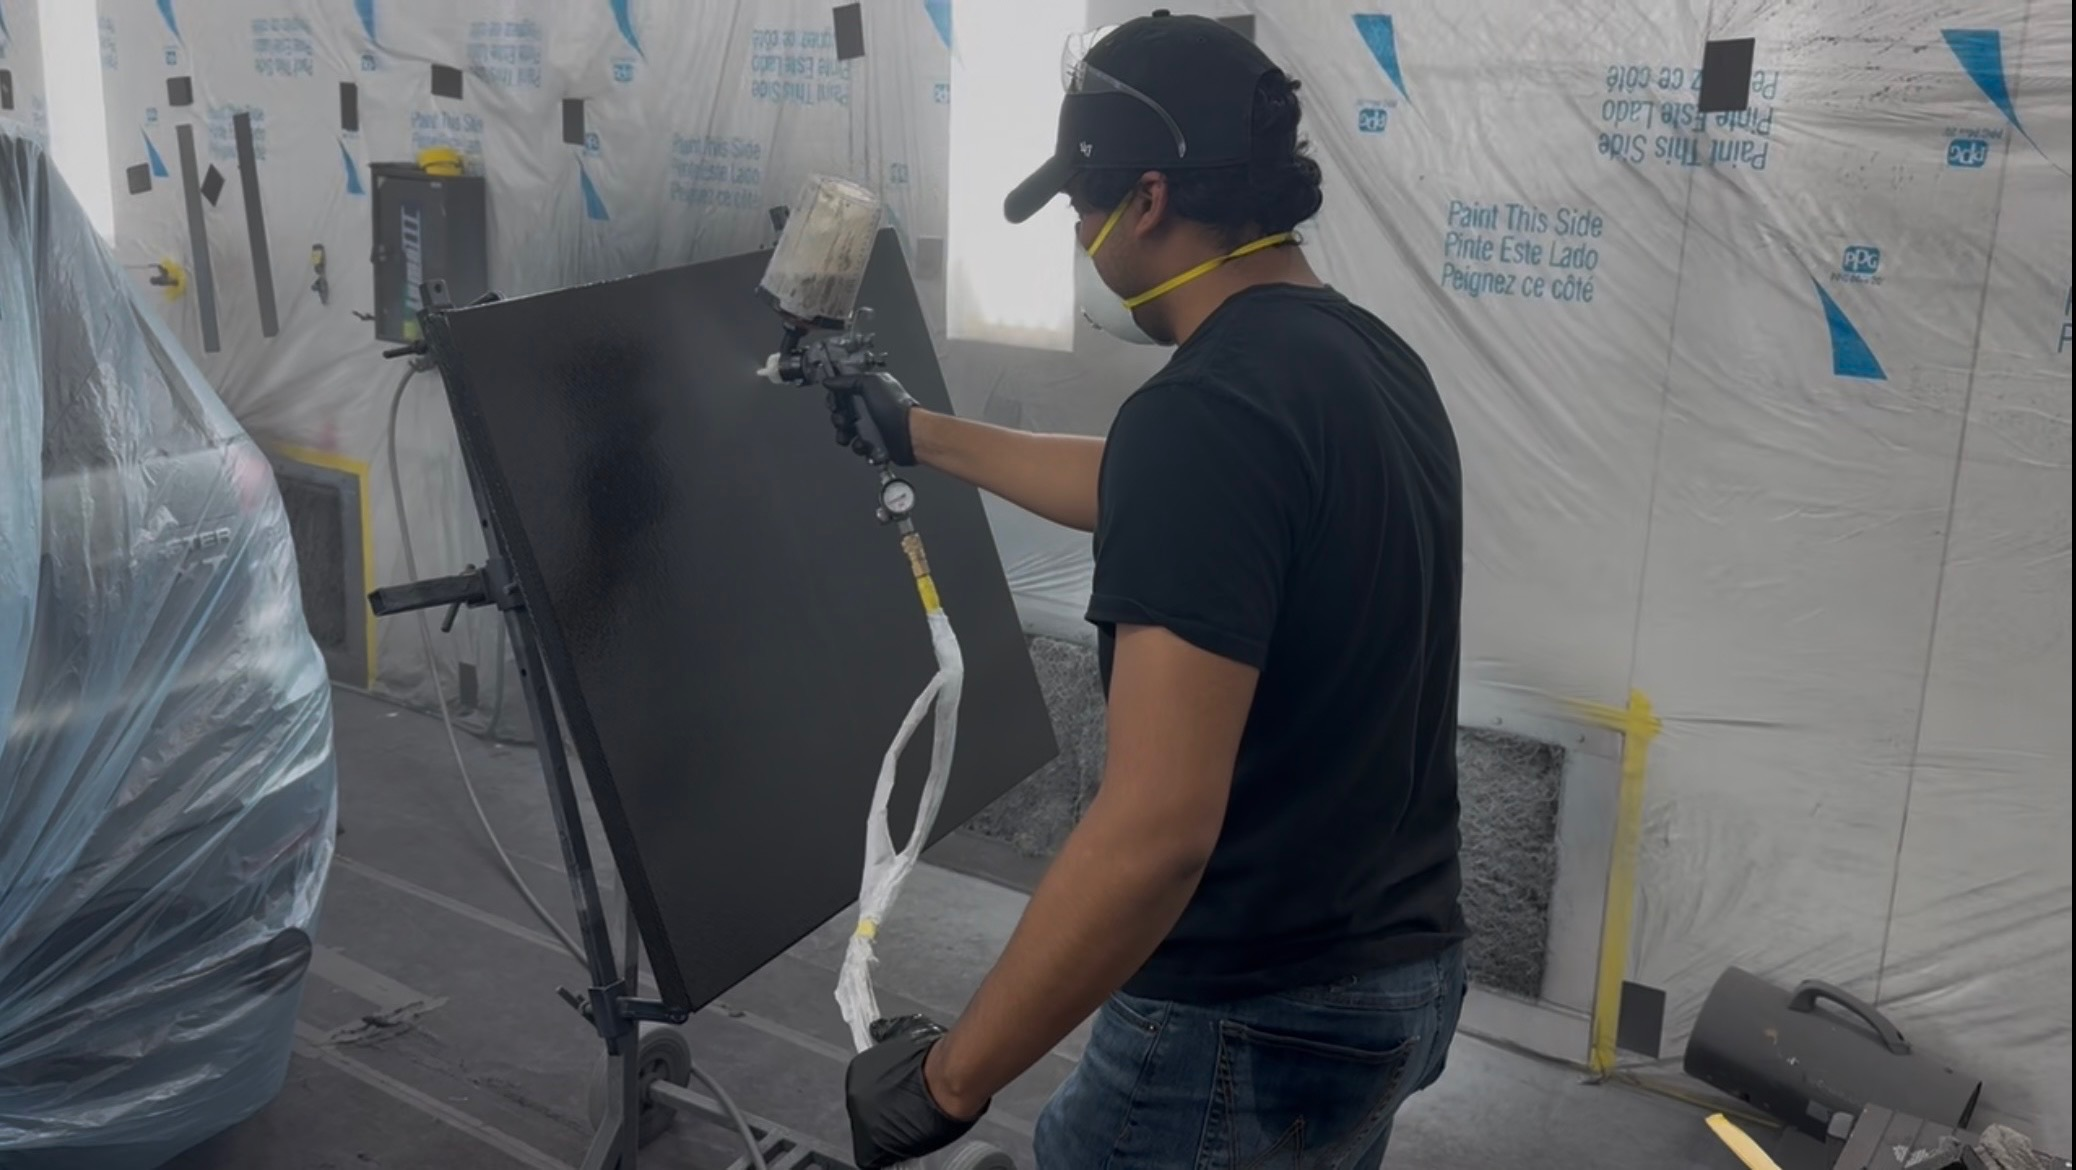
\includegraphics[
        width=2.35in,
        height=1.40in,
        keepaspectratio
    ]{spraying_topcoat}
};
\draw[RuleGray,line width=0.55pt,rounded corners=4pt]
    ($(current page.north west)+(3.10in,-1.91in)$)
    rectangle
    ($(current page.north west)+(5.65in,-3.40in)$);

% Image 3
\node[anchor=center,inner sep=0pt]
at ($(current page.north west)+(7.045in,-2.655in)$)
{
    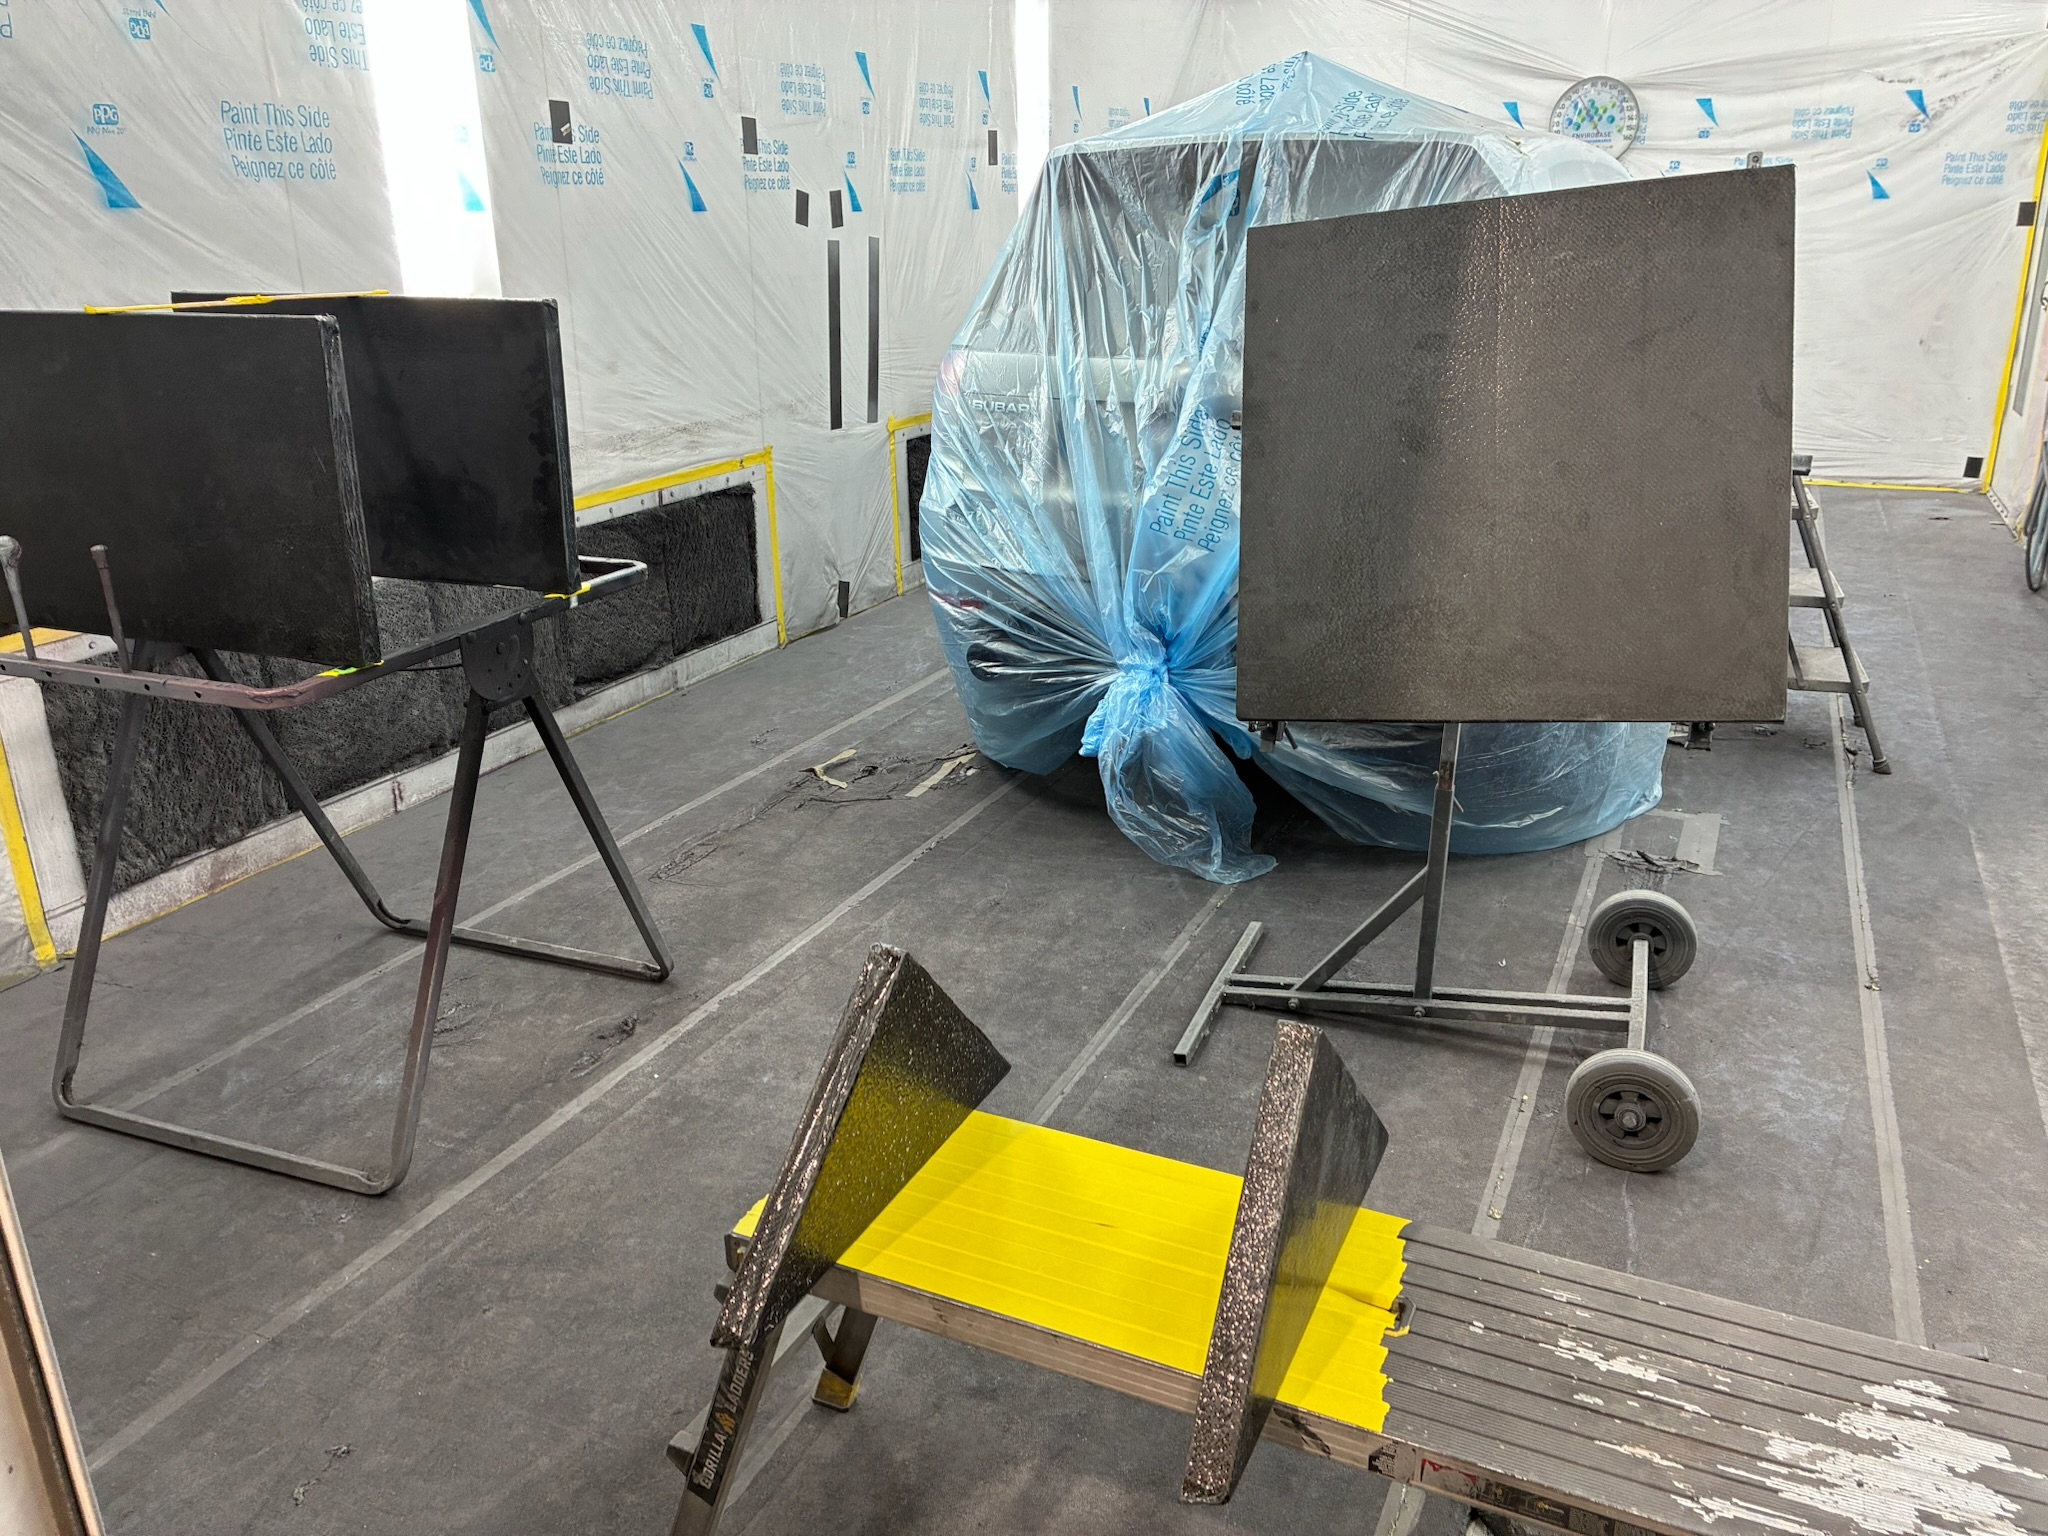
\includegraphics[
        width=2.35in,
        height=1.40in,
        keepaspectratio
    ]{topcoat_setup_apparatus}
};
\draw[RuleGray,line width=0.55pt,rounded corners=4pt]
    ($(current page.north west)+(5.77in,-1.91in)$)
    rectangle
    ($(current page.north west)+(8.32in,-3.40in)$);

% Image 4
\node[anchor=center,inner sep=0pt]
at ($(current page.north west)+(9.50in,-2.655in)$)
{
    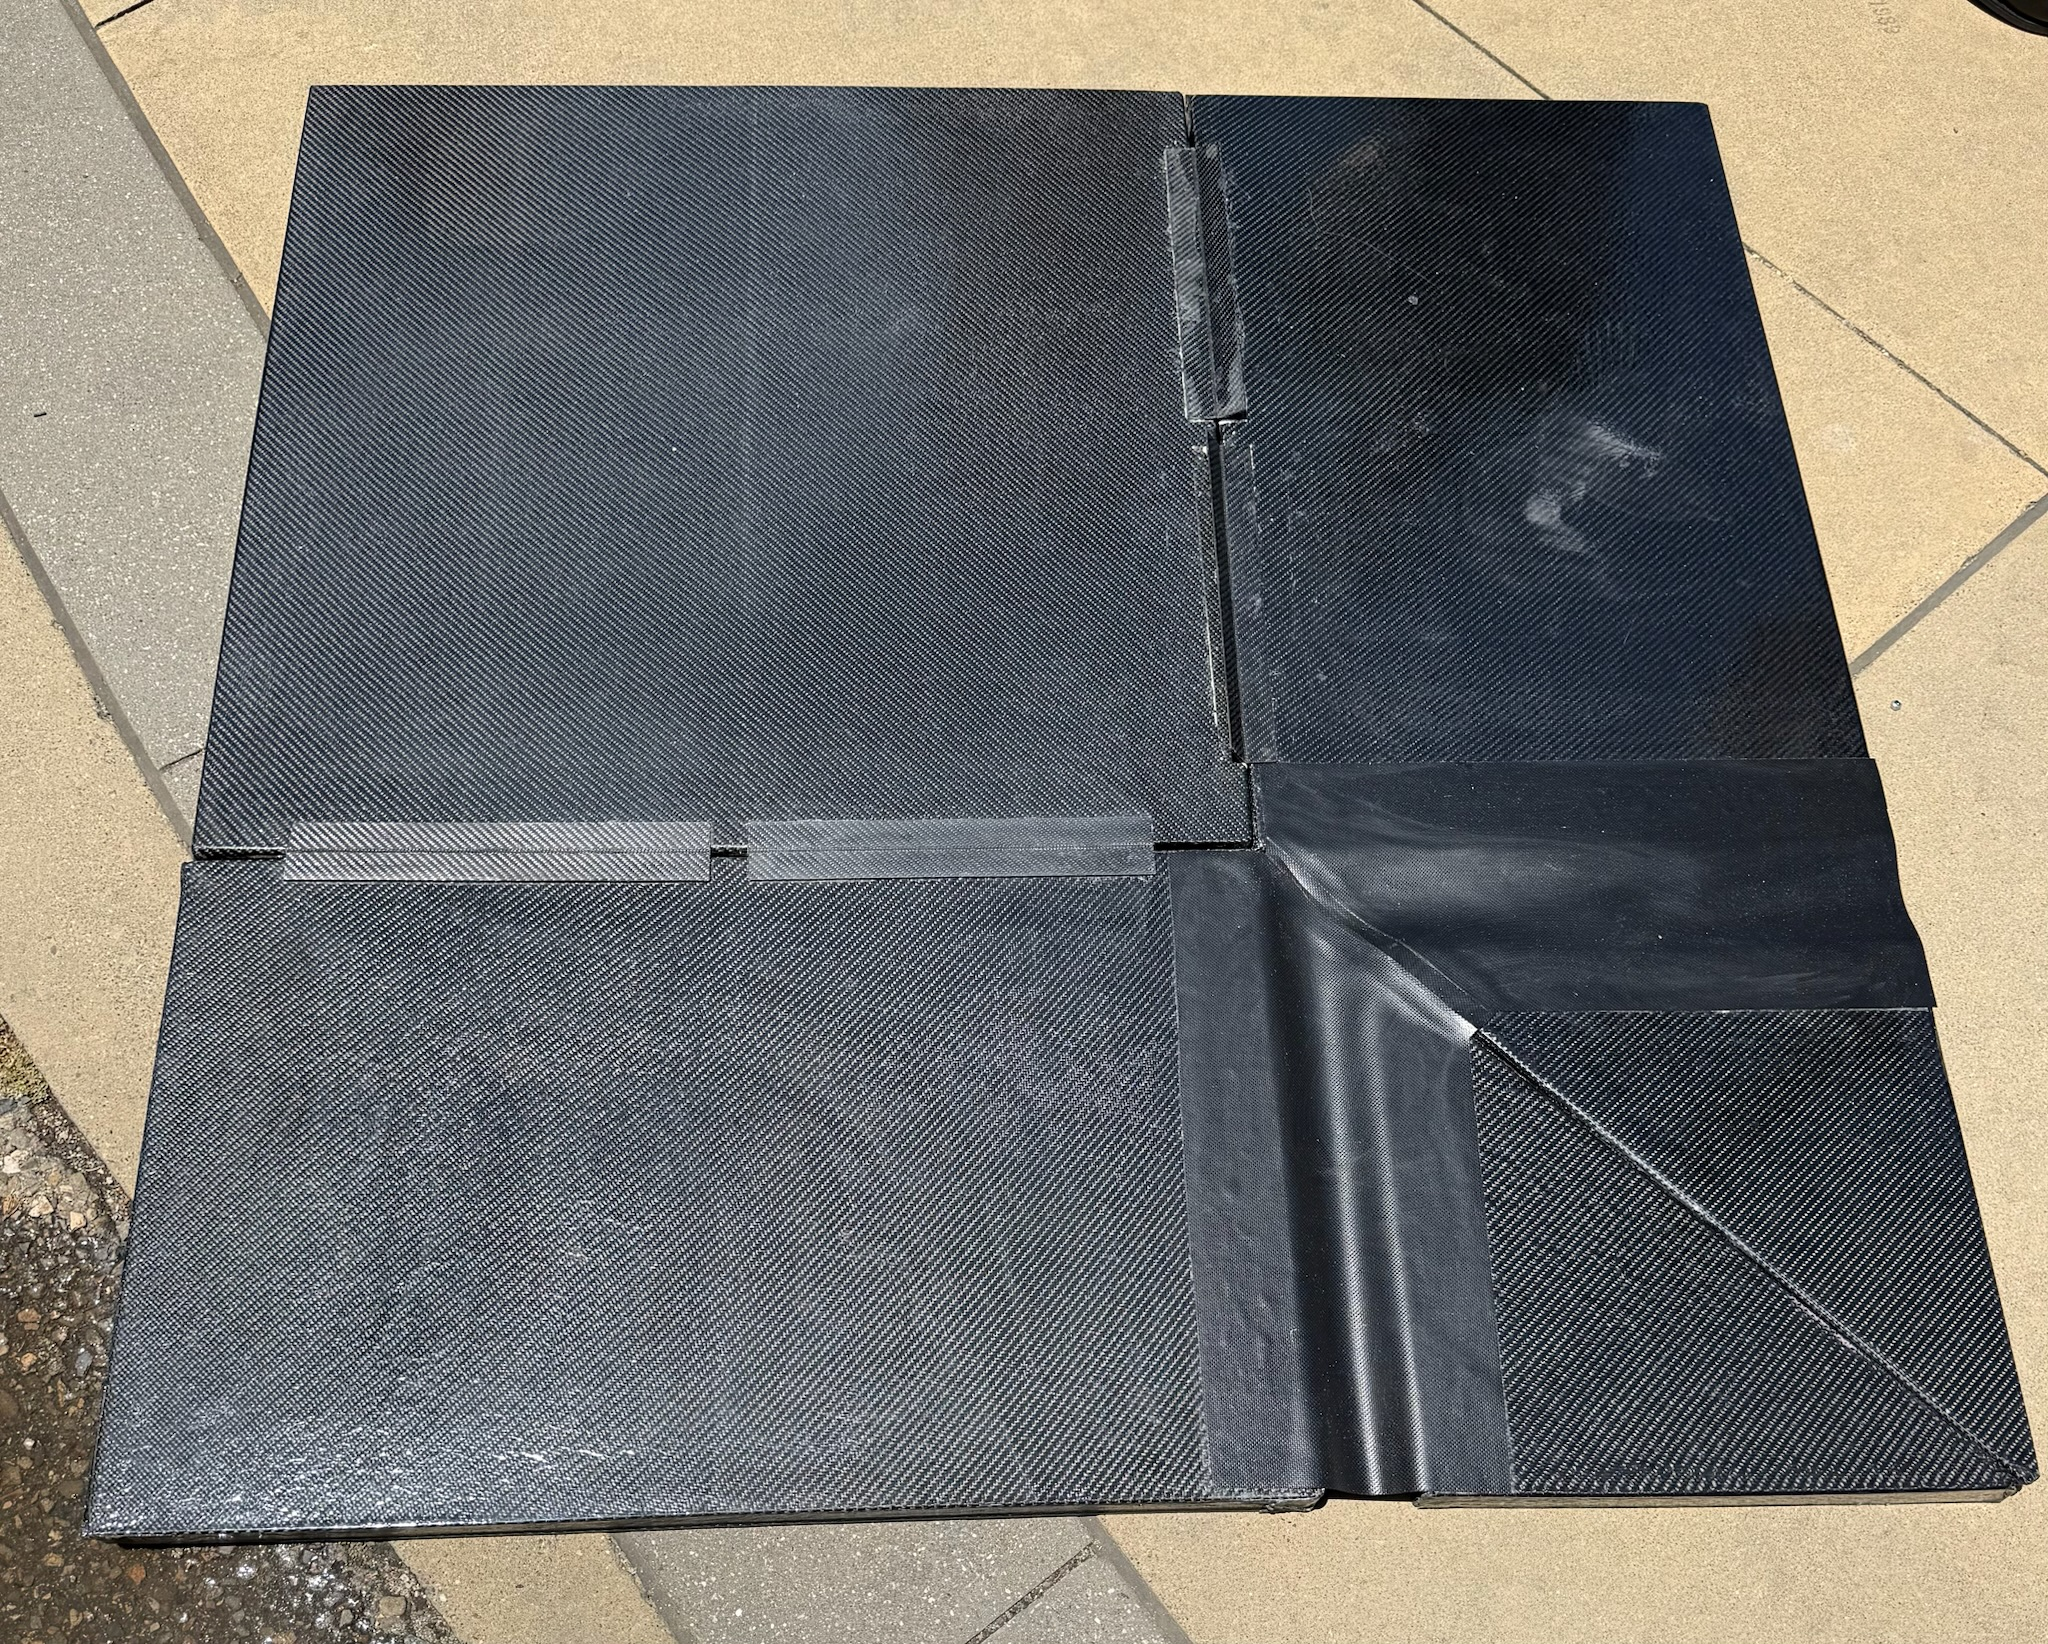
\includegraphics[
        width=2.35in,
        height=1.40in,
        keepaspectratio
    ]{refined_final_toro_cover_partial_carbon_model}
};
\draw[RuleGray,line width=0.55pt,rounded corners=4pt]
    ($(current page.north west)+(8.44in,-1.91in)$)
    rectangle
    ($(current page.north east)+(-0.42in,-3.40in)$);

% Captions
\node[anchor=north,text=Muted,font=\sffamily\fontsize{6.7}{7.3}\selectfont]
at ($(current page.north west)+(1.705in,-3.45in)$)
{Topcoat material preparation};

\node[anchor=north,text=Muted,font=\sffamily\fontsize{6.7}{7.3}\selectfont]
at ($(current page.north west)+(4.375in,-3.45in)$)
{Automotive-booth topcoat application};

\node[anchor=north,text=Muted,font=\sffamily\fontsize{6.7}{7.3}\selectfont]
at ($(current page.north west)+(7.045in,-3.45in)$)
{Coated panels drying after application};

\node[anchor=north,text=Muted,font=\sffamily\fontsize{6.7}{7.3}\selectfont]
at ($(current page.north west)+(9.50in,-3.45in)$)
{Partial carbon manufacturing model};

% Environmental rationale
\fill[SoftGold,rounded corners=4pt]
    ($(current page.north west)+(0.43in,-3.73in)$)
    rectangle
    ($(current page.north east)+(-0.42in,-4.76in)$);

\node[
    anchor=north west,
    align=left,
    text width=9.75in,
    text=Ink,
    font=\fontsize{7.05}{8.25}\selectfont
]
at ($(current page.north west)+(0.65in,-3.89in)$)
{
Because the sponsor required a carbon-fiber cover for outdoor use near chlorinated water,
environmental protection became a functional requirement rather than a cosmetic finish.
I selected and personally sprayed a UV-resistant Sunshield topcoat to seal minor laminate
porosity, reduce moisture ingress, preserve the carbon appearance, limit UV degradation of
the epoxy matrix, and isolate the composite surface from nearby metallic hardware.
};

% Results title
\node[
    anchor=north west,
    text=DeepGreen,
    font=\sffamily\bfseries\fontsize{8.0}{8.7}\selectfont
]
at ($(current page.north west)+(0.43in,-4.94in)$)
{FUNCTIONAL PROTOTYPE RESULTS};

% ------------------------------------------------------------
% Matched lower panels — larger type and improved allocation
% ------------------------------------------------------------

% Left results panel
\fill[SoftGreen,rounded corners=5pt]
    ($(current page.north west)+(0.43in,-5.22in)$)
    rectangle
    ($(current page.north west)+(5.98in,-7.39in)$);

\draw[RuleGray,line width=0.65pt,rounded corners=5pt]
    ($(current page.north west)+(0.43in,-5.22in)$)
    rectangle
    ($(current page.north west)+(5.98in,-7.39in)$);

\fill[DeepGreen,rounded corners=5pt]
    ($(current page.north west)+(0.43in,-5.22in)$)
    rectangle
    ($(current page.north west)+(5.98in,-5.58in)$);

\fill[DeepGreen]
    ($(current page.north west)+(0.43in,-5.40in)$)
    rectangle
    ($(current page.north west)+(5.98in,-5.58in)$);

\node[anchor=west,text=white,
      font=\sffamily\bfseries\fontsize{7.0}{7.6}\selectfont]
at ($(current page.north west)+(0.66in,-5.40in)$)
{SPECIFICATION};

\node[anchor=west,text=white,
      font=\sffamily\bfseries\fontsize{7.0}{7.6}\selectfont]
at ($(current page.north west)+(3.02in,-5.40in)$)
{RESULT};

\node[anchor=east,text=white,
      font=\sffamily\bfseries\fontsize{7.0}{7.6}\selectfont]
at ($(current page.north west)+(5.55in,-5.40in)$)
{STATUS};

\node[
    anchor=north west,
    align=left,
    text width=2.15in,
    text=Ink,
    font=\bfseries\fontsize{7.15}{8.55}\selectfont
]
at ($(current page.north west)+(0.66in,-5.72in)$)
{
Deployment time\\[3.4pt]
Removal time\\[3.4pt]
Single-user operation\\[3.4pt]
Single-side operation\\[3.4pt]
Deployment steps\\[3.4pt]
Removal steps\\[3.4pt]
Weight\\[3.4pt]
Folded storage
};

\node[
    anchor=north west,
    align=left,
    text width=1.45in,
    text=Ink,
    font=\fontsize{7.15}{8.55}\selectfont
]
at ($(current page.north west)+(3.02in,-5.72in)$)
{
25.51 seconds\\[3.4pt]
37.22 seconds\\[3.4pt]
100\% successful\\[3.4pt]
75\% successful\\[3.4pt]
6.4 average\\[3.4pt]
9 average\\[3.4pt]
17 lb\\[3.4pt]
2.9' x 2.9' x 1.7'
};

\node[
    anchor=north east,
    align=right,
    text width=1.05in,
    text=DeepGreen,
    font=\sffamily\bfseries\fontsize{7.05}{8.55}\selectfont
]
at ($(current page.north west)+(5.55in,-5.72in)$)
{
PASS\\[3.4pt]
PASS\\[3.4pt]
PASS\\[3.4pt]
NEAR TARGET\\[3.4pt]
PASS\\[3.4pt]
PASS\\[3.4pt]
NEAR TARGET\\[3.4pt]
PASS
};

% Right takeaways panel — widened for easier reading
\fill[SoftGreen,rounded corners=5pt]
    ($(current page.north west)+(6.14in,-5.22in)$)
    rectangle
    ($(current page.north east)+(-0.42in,-7.39in)$);

\draw[RuleGray,line width=0.65pt,rounded corners=5pt]
    ($(current page.north west)+(6.14in,-5.22in)$)
    rectangle
    ($(current page.north east)+(-0.42in,-7.39in)$);

\fill[DeepGreen,rounded corners=5pt]
    ($(current page.north west)+(6.14in,-5.22in)$)
    rectangle
    ($(current page.north east)+(-0.42in,-5.58in)$);

\fill[DeepGreen]
    ($(current page.north west)+(6.14in,-5.40in)$)
    rectangle
    ($(current page.north east)+(-0.42in,-5.58in)$);

\node[anchor=west,text=white,
      font=\sffamily\bfseries\fontsize{7.1}{7.7}\selectfont]
at ($(current page.north west)+(6.38in,-5.40in)$)
{ENGINEERING TAKEAWAYS};

\node[
    anchor=north west,
    align=left,
    text width=4.02in,
    text=Ink,
    font=\fontsize{6.75}{7.85}\selectfont
]
at ($(current page.north west)+(6.38in,-5.72in)$)
{
\textbf{Manufacturing first.}
Composite manufacturing constraints should guide the product architecture from the beginning.\\[4.5pt]
\textbf{Prioritize deliberately.}
Competing requirements must be balanced intentionally instead of maximizing every objective.\\[4.5pt]
\textbf{Lead through the process.}
Clear procedures, calm communication, and respect for teammates' strengths were essential during fabrication.\\[4.5pt]
\textbf{Next iteration.}
Reduce weight, refine the fabric-hinge fold lines, and improve panel-edge clearance.
};

% Compact concluding pathway
\node[
    anchor=center,
    align=center,
    text=PolyGold,
    font=\sffamily\bfseries\fontsize{6.3}{6.9}\selectfont
]
at ($(current page.north)+(3.06in,-7.18in)$)
{PROTOTYPE \faArrowRight\ DESIGN REFINEMENT
\faArrowRight\ REPEATABLE MANUFACTURING
\faArrowRight\ PRODUCT};

% Validation resources
\node[
    anchor=north,
    align=center,
    text=DeepGreen,
    font=\sffamily\bfseries\fontsize{6.6}{7.2}\selectfont
]
at ($(current page.north)+(0,-7.58in)$)
{\href{\ToroDeploymentLink}{\faPlayCircle\ DEPLOYMENT}
\hspace{18pt}
\href{\ToroRemovalLink}{\faPlayCircle\ REMOVAL / FOLDING}
\hspace{18pt}
\href{\ToroPosterLink}{\faFilePdf\ EXPO POSTER}
\hspace{18pt}
\href{\ToroReportLink}{\faFilePdf\ FINAL REPORT}};

% Footer
\node[
    anchor=south west,
    text=white,
    font=\sffamily\bfseries\fontsize{7.1}{7.7}\selectfont
]
at ($(current page.south west)+(0.42in,0.17in)$)
{\faArrowLeft\ MANUFACTURING-DRIVEN DESIGN};

\node[
    anchor=south,
    text=white,
    font=\sffamily\fontsize{7.0}{7.6}\selectfont
]
at ($(current page.south)+(0,0.17in)$)
{TORO COVER \hspace{6pt} 3 / 3};

\node[
    anchor=south east,
    text=white,
    font=\sffamily\bfseries\fontsize{7.1}{7.7}\selectfont
]
at ($(current page.south east)+(-0.42in,0.17in)$)
{NEXT PROJECT \faArrowRight};

\end{tikzpicture}

% ============================================================
% PICKLEBALL PADDLE — SINGLE-PAGE PORTFOLIO CASE STUDY
% Project 02 in the Composites section
%
% IMPORTANT:
% 1. This file must NOT contain \documentclass, \begin{document},
%    or \end{document}.
% 2. In main.tex, place \input{pickleball} before \end{document}.
% 3. Image references use these Overleaf base filenames:
%       waterjet
%       side_core_view
%       full_assy
%       front_view
%       LAMINATE
% ============================================================

% Clickable project resource
\providecommand{\PaddleWaterjetVideo}
{https://drive.google.com/file/d/1mTuaE_g5mE2f7Nn3R5k7yFxqCWH_pvBh/view?usp=drive_link}

\clearpage
\thispagestyle{empty}
\hypertarget{pickleball}{}
\null

\begin{tikzpicture}[remember picture,overlay]

% ============================================================
% BACKGROUND AND PAGE BARS
% ============================================================

\fill[white]
    (current page.south west)
    rectangle
    (current page.north east);

\fill[DeepGreen]
    (current page.north west)
    rectangle
    ($(current page.north east)+(0,-0.095in)$);

\fill[PolyGold]
    ($(current page.north west)+(0,-0.095in)$)
    rectangle
    ($(current page.north east)+(0,-0.14in)$);

\fill[DeepGreen]
    (current page.south west)
    rectangle
    ($(current page.south east)+(0,0.36in)$);

\fill[PolyGold]
    ($(current page.south west)+(0,0.36in)$)
    rectangle
    ($(current page.south east)+(0,0.405in)$);

% ============================================================
% HEADER
% ============================================================

\node[
    anchor=north west,
    text=PolyGold,
    font=\sffamily\bfseries\fontsize{8.1}{8.7}\selectfont
]
at ($(current page.north west)+(0.42in,-0.39in)$)
{01 COMPOSITES \hspace{5pt}/\hspace{5pt} PROJECT 02};

\node[
    anchor=north west,
    text=DeepGreen,
    font=\bfseries\fontsize{22.5}{23.5}\selectfont
]
at ($(current page.north west)+(0.40in,-0.67in)$)
{CARBON FIBER PICKLEBALL PADDLE};

\node[
    anchor=north west,
    text=Muted,
    font=\sffamily\fontsize{8.4}{9.2}\selectfont
]
at ($(current page.north west)+(0.42in,-1.12in)$)
{Cal Poly Composites Laboratory \hspace{7pt}\textbullet\hspace{7pt}
Individual Project \hspace{7pt}\textbullet\hspace{7pt}
Spring 2026 \hspace{7pt}\textbullet\hspace{7pt}
San Luis Obispo, California};

\fill[PolyGold]
    ($(current page.north west)+(0.42in,-1.36in)$)
    rectangle
    ($(current page.north west)+(6.10in,-1.315in)$);

% ============================================================
% TOP LEFT — HERO PRODUCT IMAGE
% ============================================================

\node[
    anchor=center,
    inner sep=3pt,
    draw=DeepGreen,
    line width=0.75pt,
    rounded corners=6pt
]
at ($(current page.north west)+(1.60in,-3.20in)$)
{
    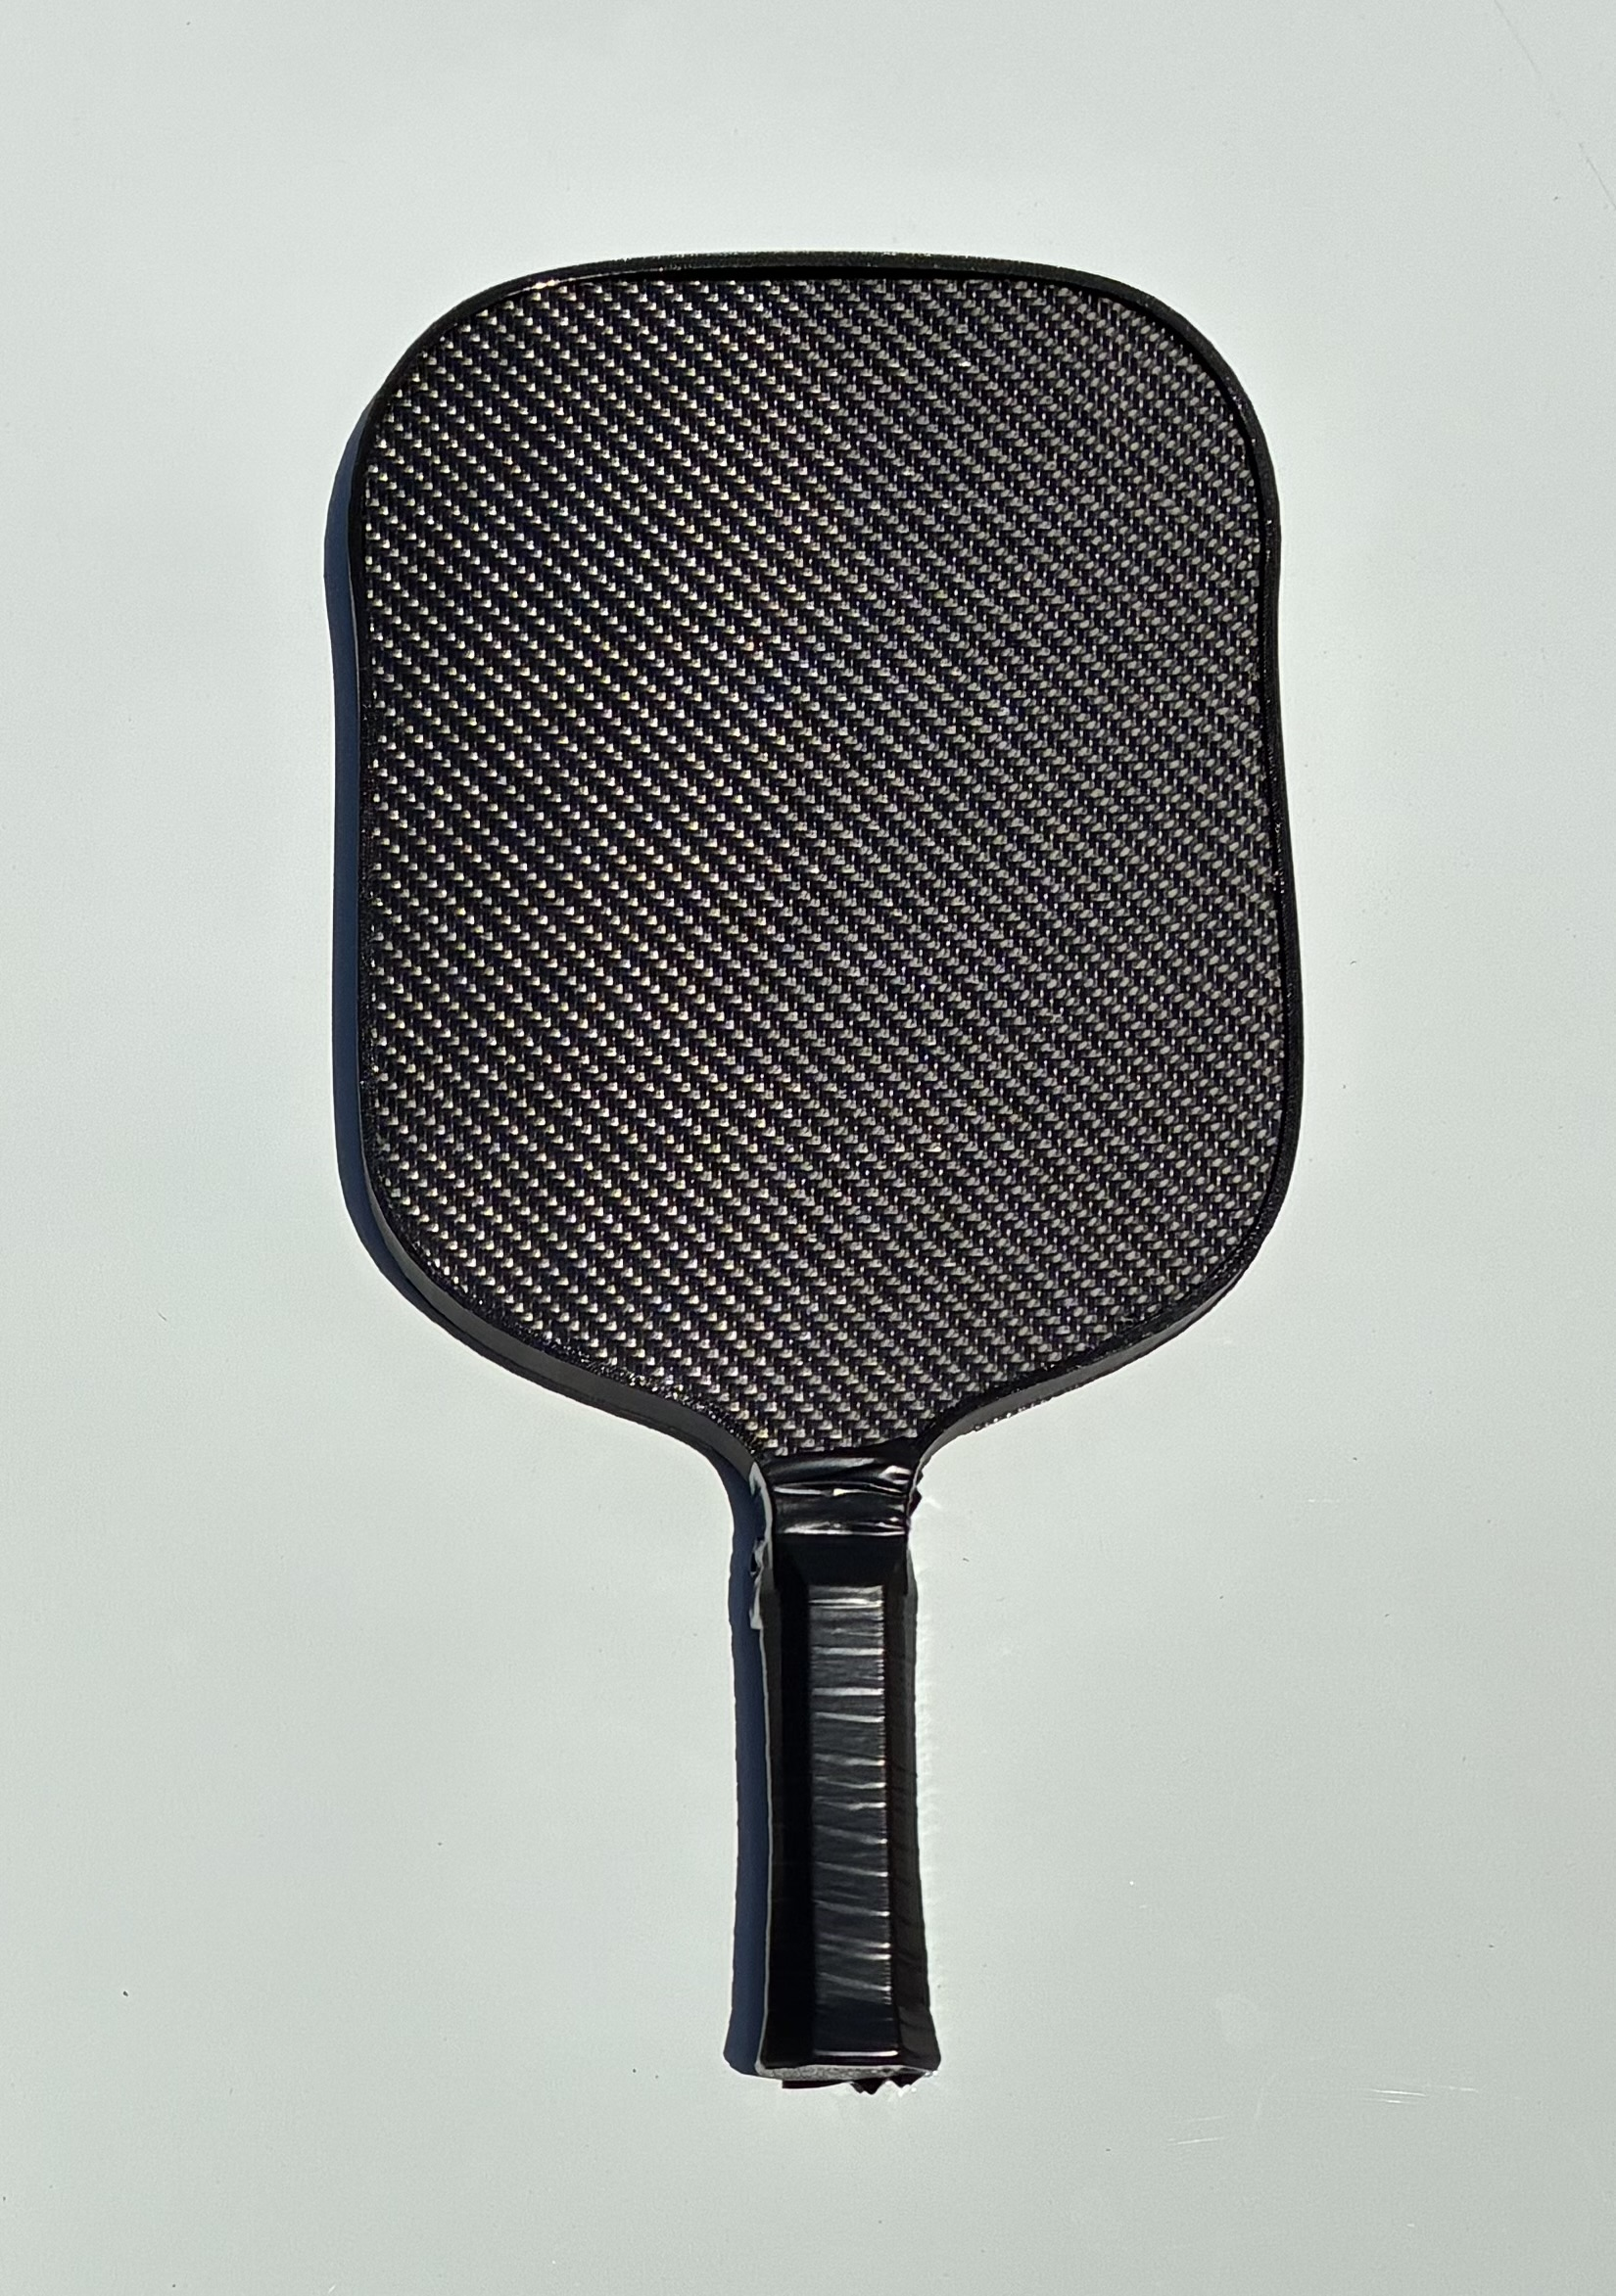
\includegraphics[
        width=3.72in,
        height=3.18in,
        keepaspectratio
    ]{full_assy}
};

\node[
    anchor=north,
    text=Muted,
    font=\sffamily\fontsize{6.9}{7.5}\selectfont
]
at ($(current page.north west)+(1.60in,-4.86in)$)
{Completed solo-built paddle assembly};

% ============================================================
% TOP CENTER — PROJECT OVERVIEW
% ============================================================

\fill[SoftGold,rounded corners=5pt]
    ($(current page.north west)+(2.95in,-1.62in)$)
    rectangle
    ($(current page.north west)+(5.53in,-4.86in)$);

\fill[PolyGold]
    ($(current page.north west)+(2.95in,-1.62in)$)
    rectangle
    ($(current page.north west)+(3.05in,-4.86in)$);

\node[
    anchor=north west,
    text=DeepGreen,
    font=\sffamily\bfseries\fontsize{8.0}{8.7}\selectfont
]
at ($(current page.north west)+(3.23in,-1.79in)$)
{PROJECT OVERVIEW};

\node[
    anchor=north west,
    align=left,
    text width=2.02in,
    text=Ink,
    font=\fontsize{7.05}{8.35}\selectfont
]
at ($(current page.north west)+(3.23in,-2.07in)$)
{
Independently designed and manufactured a lightweight prepreg
carbon-fiber pickleball paddle using a half-inch honeycomb
sandwich core, vacuum-bag consolidation, precision waterjet
trimming, and custom TPU and PLA components.

\vspace{5pt}

The project emphasized lightweight sandwich-composite design, repeatable manufacturing methods, dimensional accuracy, and the integration of custom 3D-printed TPU and PLA components into the final assembly.
};

\node[
    anchor=south west,
    align=left,
    text width=2.02in,
    text=PolyGold,
    font=\sffamily\bfseries\fontsize{6.65}{7.35}\selectfont
]
at ($(current page.north west)+(3.23in,-4.74in)$)
{
SOLE DESIGNER\\[2pt]
COMPOSITE FABRICATOR\\[2pt]
MANUFACTURING ENGINEER
};

% ============================================================
% TOP RIGHT — LAMINATE GRAPHIC
% ============================================================

\node[
    anchor=north west,
    inner sep=2.5pt,
    draw=DeepGreen,
    line width=0.65pt,
    rounded corners=5pt
]
at ($(current page.north west)+(5.71in,-1.62in)$)
{
    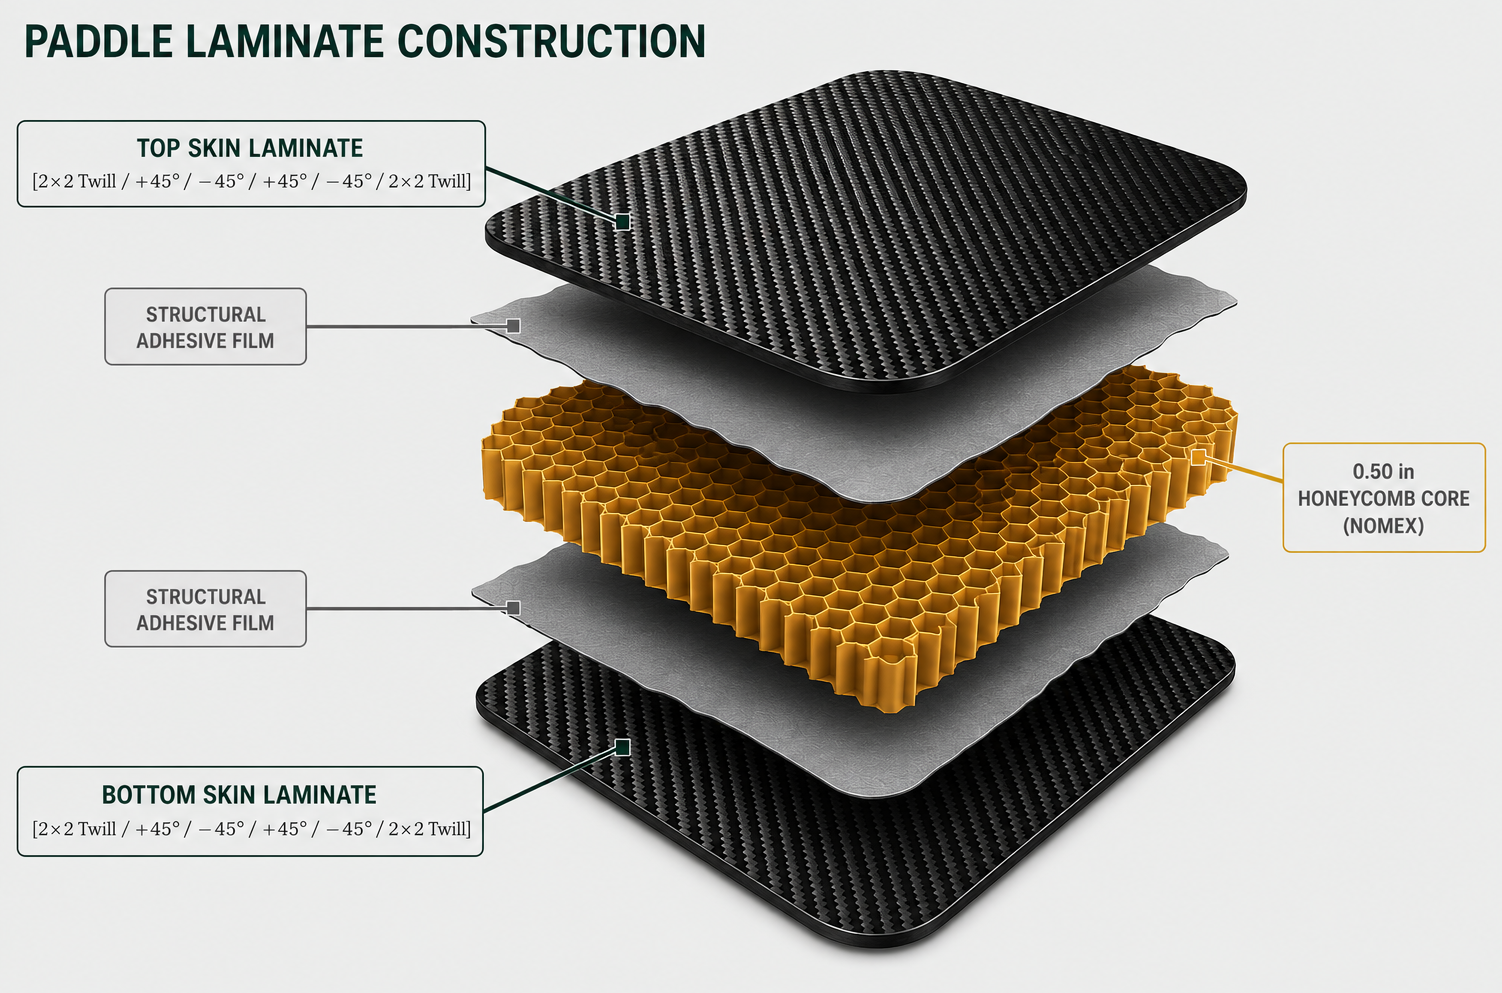
\includegraphics[
        width=4.80in,
        keepaspectratio
    ]{LAMINATE}
};

% ============================================================
% BOTTOM LEFT — SUPPORTING IMAGES
% ============================================================

\node[
    anchor=center,
    inner sep=3pt,
    draw=RuleGray,
    line width=0.55pt,
    rounded corners=4pt
]
at ($(current page.north west)+(1.12in,-5.98in)$)
{
    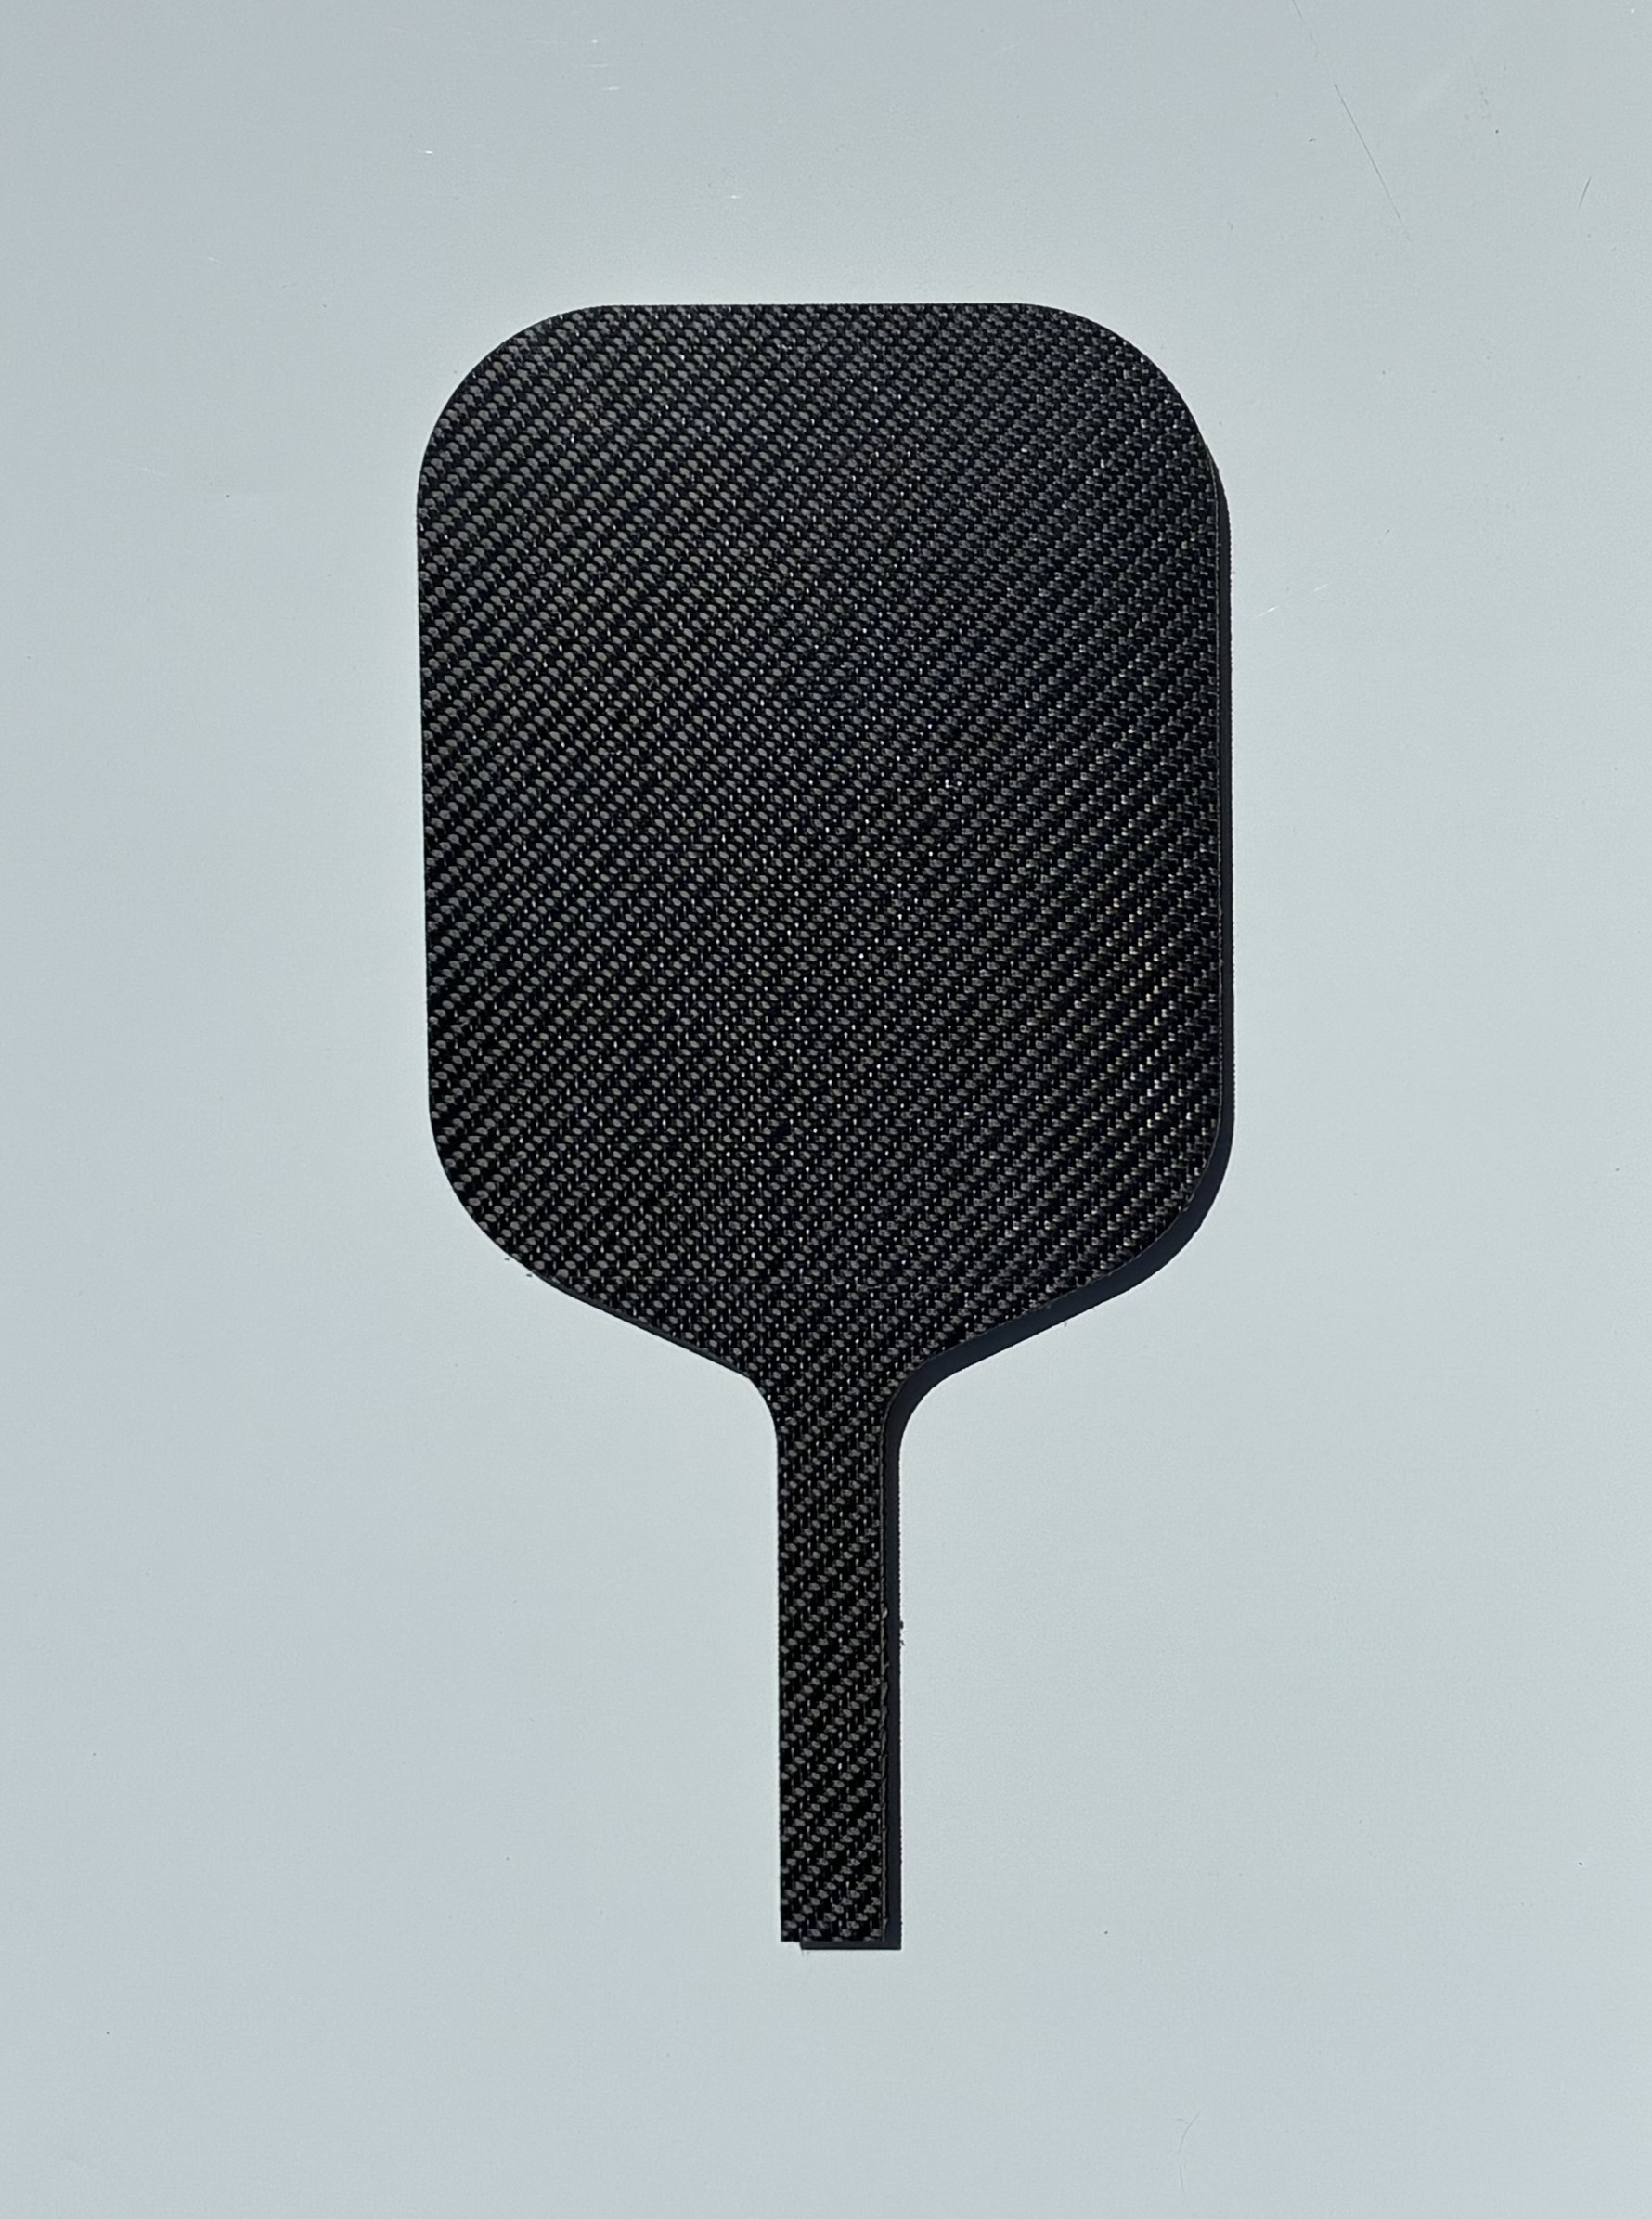
\includegraphics[
        width=1.30in,
        height=1.78in,
        keepaspectratio
    ]{front_view}
};

\node[
    anchor=center,
    inner sep=3pt,
    draw=RuleGray,
    line width=0.55pt,
    rounded corners=4pt
]
at ($(current page.north west)+(2.72in,-5.98in)$)
{
    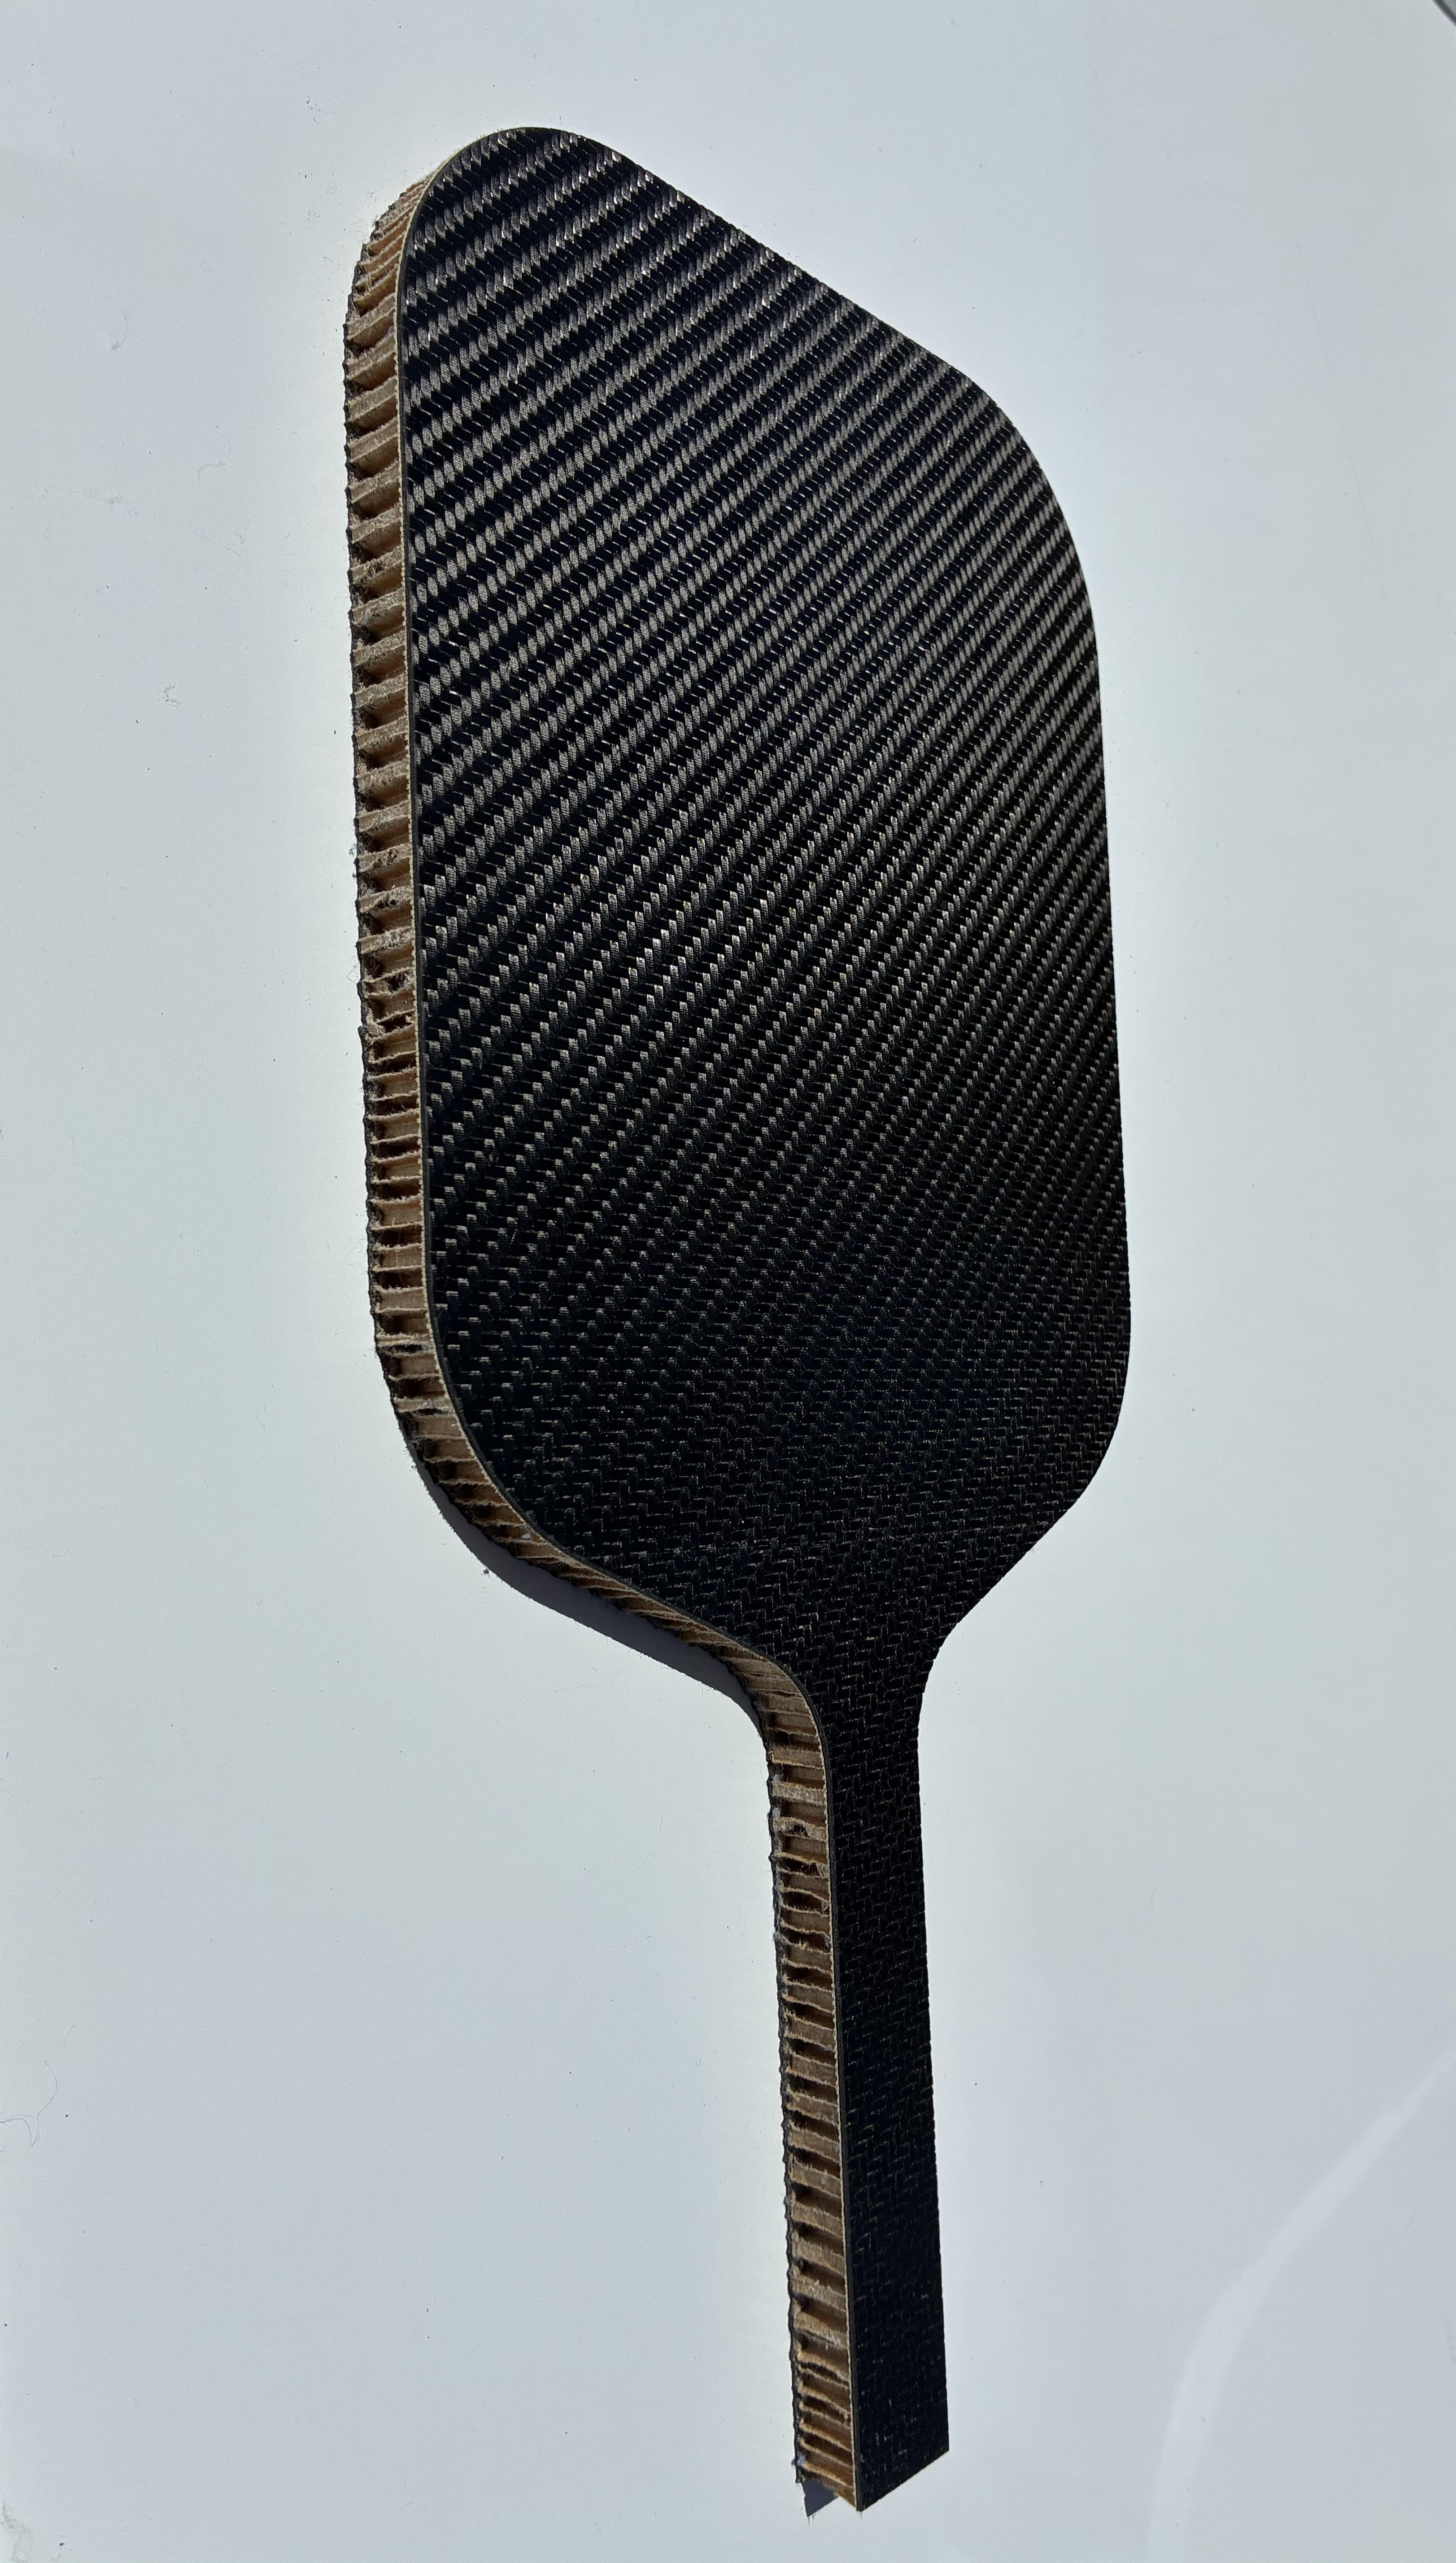
\includegraphics[
        width=1.30in,
        height=1.78in,
        keepaspectratio
    ]{side_core_view}
};

\node[
    anchor=center,
    inner sep=3pt,
    draw=RuleGray,
    line width=0.55pt,
    rounded corners=4pt
]
at ($(current page.north west)+(4.32in,-5.98in)$)
{
    \includegraphics[
        angle=-90,
        origin=c,
        width=1.30in,
        height=1.78in,
        keepaspectratio
    ]{waterjet}
};

\node[
    anchor=north,
    align=center,
    text width=1.38in,
    text=Muted,
    font=\sffamily\fontsize{6.5}{7.1}\selectfont
]
at ($(current page.north west)+(1.12in,-7.00in)$)
{Front view};

\node[
    anchor=north,
    align=center,
    text width=1.38in,
    text=Muted,
    font=\sffamily\fontsize{6.5}{7.1}\selectfont
]
at ($(current page.north west)+(2.72in,-7.00in)$)
{Core and edge profile};

\node[
    anchor=north,
    align=center,
    text width=1.38in,
    text=Muted,
    font=\sffamily\fontsize{6.5}{7.1}\selectfont
]
at ($(current page.north west)+(4.32in,-7.00in)$)
{Waterjet cutting setup};

% ============================================================
% BOTTOM RIGHT — MANUFACTURING HIGHLIGHTS
% ============================================================

\fill[SoftGreen,rounded corners=5pt]
    ($(current page.north west)+(5.18in,-5.05in)$)
    rectangle
    ($(current page.north east)+(-0.42in,-7.18in)$);

\draw[RuleGray,line width=0.55pt,rounded corners=5pt]
    ($(current page.north west)+(5.18in,-5.05in)$)
    rectangle
    ($(current page.north east)+(-0.42in,-7.18in)$);

\node[
    anchor=north west,
    text=DeepGreen,
    font=\sffamily\bfseries\fontsize{7.9}{8.6}\selectfont
]
at ($(current page.north west)+(5.44in,-5.20in)$)
{MANUFACTURING HIGHLIGHTS};

\node[
    anchor=north west,
    align=left,
    text width=5.05in,
    text=Ink,
    font=\fontsize{6.72}{7.82}\selectfont
]
at ($(current page.north west)+(5.44in,-5.49in)$)
{
\textbf{Consolidation.}
Vacuum bagging and distributed weight pressure maintained intimate contact
throughout the prepreg sandwich layup.\\[2.4pt]
\textbf{Surface quality.}
A scarce PTFE release film produced an unusually consistent matte finish
with a subtle sheen and minimal post-processing.\\[2.4pt]
\textbf{Waterjet stability.}
Perimeter weights restrained the cured stock against jet-induced lifting
and rotational moments during cutting.\\[2.4pt]
\textbf{Final assembly.}
A printed TPU edge band protected the carbon perimeter, while the PLA handle
used clearance cutouts to accommodate future stock-thickness and cutting variation.
};

% ============================================================
% RESOURCE LINK
% ============================================================

\node[
    anchor=north,
    align=center,
    text=DeepGreen,
    font=\sffamily\bfseries\fontsize{7.0}{7.6}\selectfont
]
at ($(current page.north)+(0,-7.42in)$)
{\href{\PaddleWaterjetVideo}
{\faPlayCircle\ WATERJET PICKLEBALL PADDLE DEMONSTRATION}};

% ============================================================
% FOOTER
% ============================================================

\node[
    anchor=south west,
    text=white,
    font=\sffamily\bfseries\fontsize{7.1}{7.7}\selectfont
]
at ($(current page.south west)+(0.42in,0.17in)$)
{\hyperlink{toro-results}{\faArrowLeft\ TORO COVER}};

\node[
    anchor=south,
    text=white,
    font=\sffamily\fontsize{7.0}{7.6}\selectfont
]
at ($(current page.south)+(0,0.17in)$)
{PICKLEBALL PADDLE \hspace{6pt} 1 / 1};

\node[
    anchor=south east,
    text=white,
    font=\sffamily\bfseries\fontsize{7.1}{7.7}\selectfont
]
at ($(current page.south east)+(-0.42in,0.17in)$)
{NEXT PROJECT \faArrowRight};

\end{tikzpicture}
%\input{Beam}
%\clearpage

\clearpage
.
% 2. In main.tex, place 
% ============================================================
% TORO COVER — THREE-PAGE PORTFOLIO CASE STUDY
% Pages 3–5 of the complete portfolio
%
% IMPORTANT:
% 1. This file must NOT contain \documentclass, \begin{document},
%    \end{document}, or 
% ============================================================
% TORO COVER — THREE-PAGE PORTFOLIO CASE STUDY
% Pages 3–5 of the complete portfolio
%
% IMPORTANT:
% 1. This file must NOT contain \documentclass, \begin{document},
%    \end{document}, or \input{toro}.
% 2. In main.tex, place \input{toro} before \end{document}.
% 3. Image references use the original Overleaf base filenames
%    without extensions.
% ============================================================



% ============================================================
% CLICKABLE PROJECT RESOURCES
% All links use the exact Google Drive resources supplied.
% ============================================================
\providecommand{\ToroDrawingLink}{https://drive.google.com/file/d/1A7-7wMnRNLuQDaTgxeuUCBsGNqyXzOGV/view?usp=sharing}
\providecommand{\ToroDimensionsLink}{https://drive.google.com/file/d/13sw3BNJvE8GdzlRffxoF2n5r9Gzxide7/view?usp=sharing}
\providecommand{\ToroProblemLink}{https://drive.google.com/file/d/1zHtl8zrb13F1yeN74ptawpfS5UM_xsuw/view?usp=drive_link}
\providecommand{\ToroReportLink}{https://drive.google.com/file/d/1ULZ-P46lFsC2x29ZfmRVIKgYnr9o8hMt/view?usp=drive_link}
\providecommand{\ToroPosterLink}{https://drive.google.com/file/d/1vKiKaJUcHQb_db-FkZnRF6EvtuM4hKyS/view?usp=drive_link}
\providecommand{\ToroDeploymentLink}{https://drive.google.com/file/d/1XJx34o80_mZPTl7xy93HtWAgtS3ThhvY/view?usp=drive_link}
\providecommand{\ToroRemovalLink}{https://drive.google.com/file/d/1O7xYeyB67NUwT-j1B1HeiCcHnZDYjk6_/view?usp=drive_link}

% ============================================================
% PAGE 1 — PROJECT OVERVIEW, OWNERSHIP, AND ARCHITECTURE
% ============================================================

\clearpage
\thispagestyle{empty}
\hypertarget{toro}{}
\null

\begin{tikzpicture}[remember picture,overlay]

% Background
\fill[white]
    (current page.south west)
    rectangle
    (current page.north east);

% Page bars
\fill[DeepGreen]
    (current page.north west)
    rectangle
    ($(current page.north east)+(0,-0.095in)$);

\fill[PolyGold]
    ($(current page.north west)+(0,-0.095in)$)
    rectangle
    ($(current page.north east)+(0,-0.14in)$);

\fill[DeepGreen]
    (current page.south west)
    rectangle
    ($(current page.south east)+(0,0.36in)$);

\fill[PolyGold]
    ($(current page.south west)+(0,0.36in)$)
    rectangle
    ($(current page.south east)+(0,0.405in)$);

% Header
\node[
    anchor=north west,
    text=PolyGold,
    font=\sffamily\bfseries\fontsize{8.1}{8.7}\selectfont
]
at ($(current page.north west)+(0.42in,-0.39in)$)
{01 COMPOSITES \hspace{5pt}/\hspace{5pt} PROJECT 01};

\node[
    anchor=north west,
    text=DeepGreen,
    font=\bfseries\fontsize{23.5}{24.5}\selectfont
]
at ($(current page.north west)+(0.40in,-0.67in)$)
{TORO CARBON FIBER SAFETY COVER};

\node[
    anchor=north west,
    text=Muted,
    font=\sffamily\fontsize{8.4}{9.2}\selectfont
]
at ($(current page.north west)+(0.42in,-1.12in)$)
{Cal Poly Composites Laboratory \hspace{7pt}\textbullet\hspace{7pt}
Team Project \hspace{7pt}\textbullet\hspace{7pt}
Fall--Spring 2026 \hspace{7pt}\textbullet\hspace{7pt}
San Luis Obispo, California};

\fill[PolyGold]
    ($(current page.north west)+(0.42in,-1.37in)$)
    rectangle
    ($(current page.north west)+(6.1in,-1.325in)$);

% Challenge text
\node[
    anchor=north west,
    text=DeepGreen,
    font=\sffamily\bfseries\fontsize{8.1}{8.8}\selectfont
]
at ($(current page.north west)+(0.43in,-1.61in)$)
{THE CHALLENGE};

\node[
    anchor=north west,
    align=left,
    text width=4.47in,
    text=Ink,
    font=\fontsize{8.05}{9.65}\selectfont
]
at ($(current page.north west)+(0.43in,-1.84in)$)
{
Develop a lightweight cover for a 6 ft by 6 ft in-ground spa
that could be deployed by one person, stored compactly,
provide insulation, resist a poolside environment, and maintain
a refined appearance. The sponsor supplied an ambitious but
intentionally broad project statement, requiring the team to
define the product architecture, priorities, manufacturing
strategy, and realistic path toward future commercialization.
};

% Role box
\fill[SoftGold,rounded corners=5pt]
    ($(current page.north west)+(0.42in,-2.88in)$)
    rectangle
    ($(current page.north west)+(4.98in,-4.58in)$);

\fill[PolyGold]
    ($(current page.north west)+(0.42in,-2.88in)$)
    rectangle
    ($(current page.north west)+(0.52in,-4.58in)$);

\node[
    anchor=north west,
    text=DeepGreen,
    font=\sffamily\bfseries\fontsize{8.1}{8.8}\selectfont
]
at ($(current page.north west)+(0.66in,-3.02in)$)
{MY ROLE — DESIGN \& MANUFACTURING LEAD};

\node[
    anchor=north west,
    align=left,
    text width=4.02in,
    text=Ink,
    font=\fontsize{7.05}{8.15}\selectfont
]
at ($(current page.north west)+(0.66in,-3.27in)$)
{
\textbullet\ Modeled every custom part and the complete assembly\\[1.5pt]
\textbullet\ Produced the engineering drawing package independently\\[1.5pt]
\textbullet\ Developed the composite-panel manufacturing process\\[1.5pt]
\textbullet\ Created all waterjet DXFs and manufacturing geometry\\[1.5pt]
\textbullet\ Trained teammates in wet layup and vacuum bagging\\[1.5pt]
\textbullet\ Presented feasibility, scope, and tradeoffs to the sponsor
};

% Large deployed foam-model image
\node[anchor=center,inner sep=0pt]
at ($(current page.north west)+(8.00in,-3.04in)$)
{
    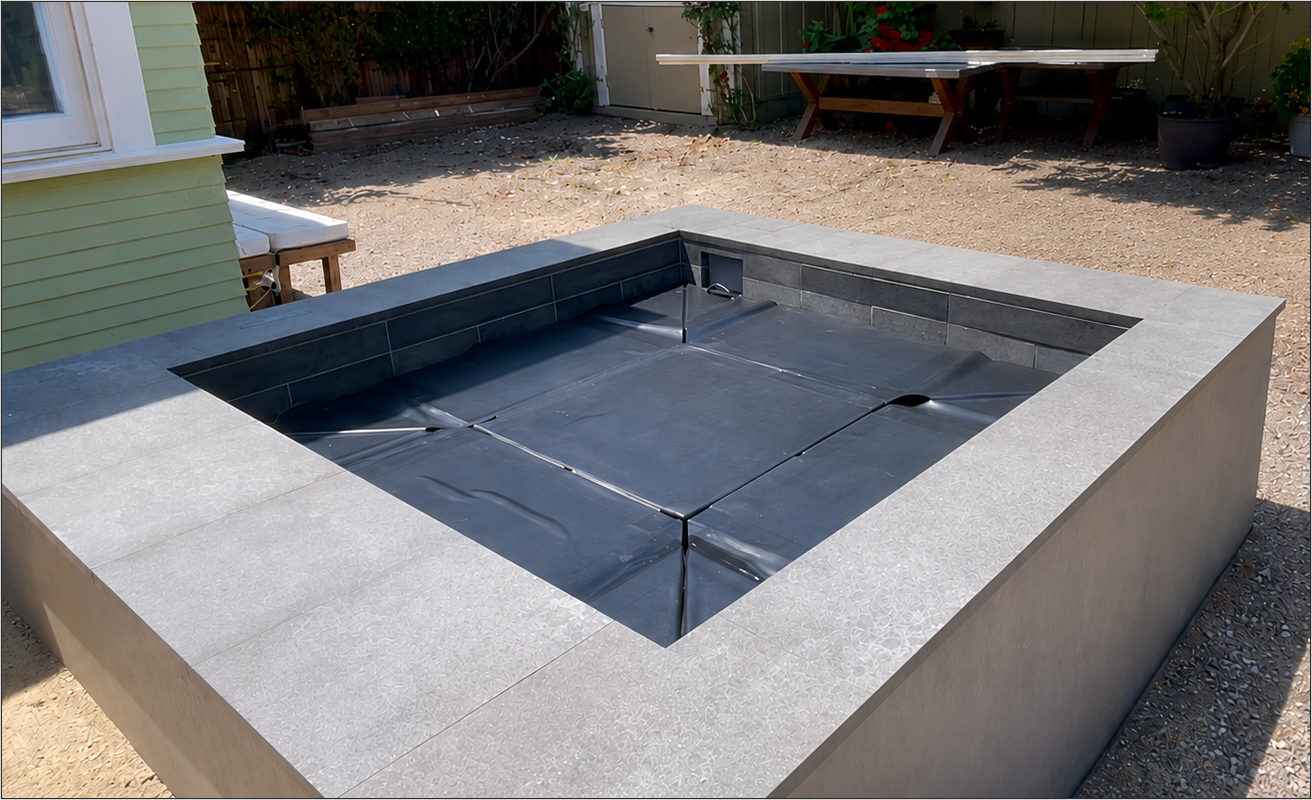
\includegraphics[
        width=5.55in,
        height=2.78in,
        keepaspectratio
    ]{deployed_functional_prototype}
};

\draw[DeepGreen,line width=0.8pt,rounded corners=7pt]
    ($(current page.north west)+(5.16in,-1.61in)$)
    rectangle
    ($(current page.north east)+(-0.42in,-4.47in)$);

\node[
    anchor=north west,
    text=Muted,
    font=\sffamily\fontsize{6.2}{6.9}\selectfont
]
at ($(current page.north west)+(5.18in,-4.54in)$)
{Functional foam model deployed over the sponsor's in-ground spa.};

% Image-strip title
\node[
    anchor=north west,
    text=DeepGreen,
    font=\sffamily\bfseries\fontsize{8.1}{8.8}\selectfont
]
at ($(current page.north west)+(0.43in,-4.78in)$)
{PRODUCT DEVELOPMENT AND FINAL ARCHITECTURE};

% Five-image development strip — CAD-first sequence
% Image 1: topside CAD
\node[anchor=center,inner sep=0pt]
at ($(current page.north west)+(1.47in,-5.73in)$)
{
    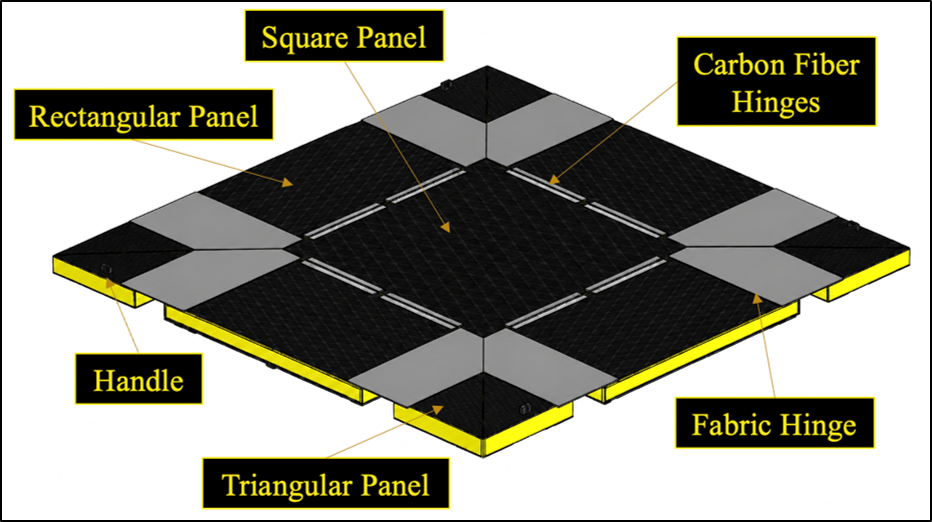
\includegraphics[
        width=1.92in,
        height=1.30in,
        keepaspectratio
    ]{Toro_Cover_topside_Cad}
};
\draw[RuleGray,line width=0.55pt,rounded corners=4pt]
    ($(current page.north west)+(0.43in,-5.04in)$)
    rectangle
    ($(current page.north west)+(2.51in,-6.43in)$);

% Image 2: underside CAD
\node[anchor=center,inner sep=0pt]
at ($(current page.north west)+(3.66in,-5.73in)$)
{
    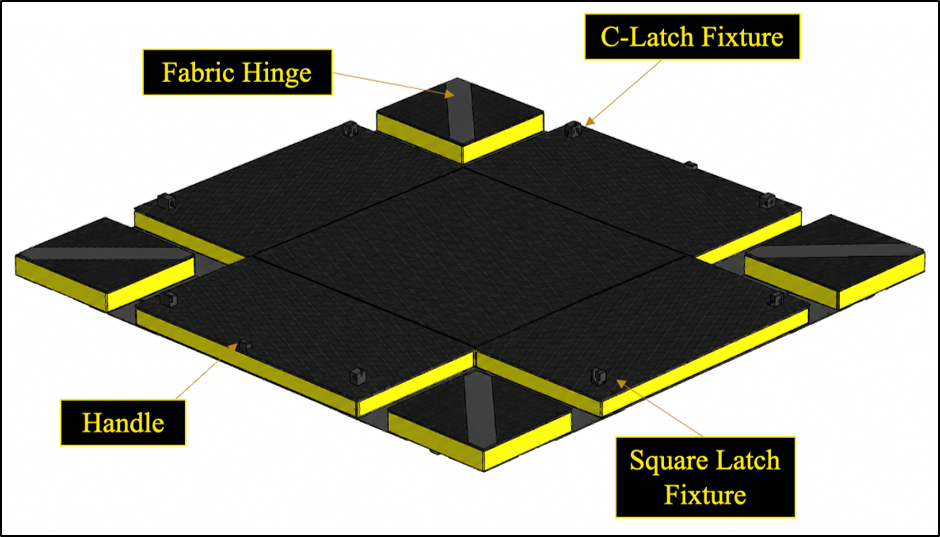
\includegraphics[
        width=1.92in,
        height=1.30in,
        keepaspectratio
    ]{toro_cover_underside_cad}
};
\draw[RuleGray,line width=0.55pt,rounded corners=4pt]
    ($(current page.north west)+(2.62in,-5.04in)$)
    rectangle
    ($(current page.north west)+(4.70in,-6.43in)$);

% Image 3: folded CAD
\node[anchor=center,inner sep=0pt]
at ($(current page.north west)+(5.85in,-5.73in)$)
{
    \includegraphics[
        width=1.92in,
        height=1.30in,
        keepaspectratio
    ]{\detokenize{Toro_Cover_folded Configuration}}
};
\draw[RuleGray,line width=0.55pt,rounded corners=4pt]
    ($(current page.north west)+(4.81in,-5.04in)$)
    rectangle
    ($(current page.north west)+(6.89in,-6.43in)$);

% Image 4: dual-use product concept
\node[anchor=center,inner sep=0pt]
at ($(current page.north west)+(8.04in,-5.73in)$)
{
    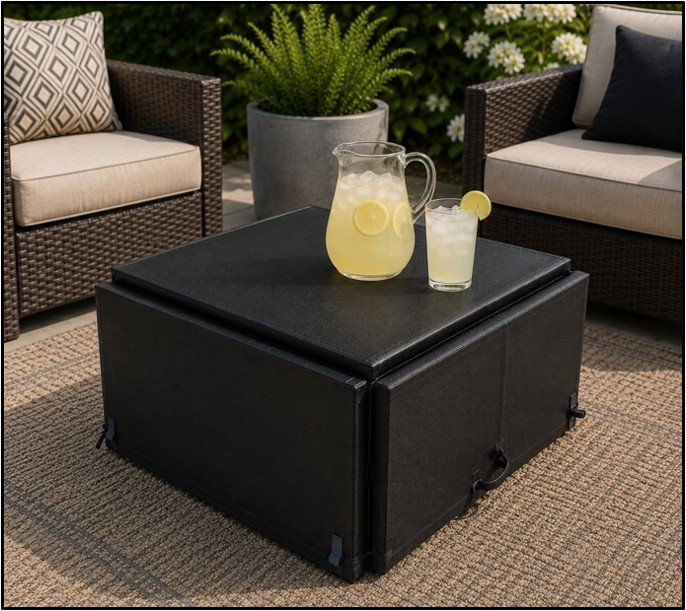
\includegraphics[
        width=1.92in,
        height=1.30in,
        keepaspectratio
    ]{generative_AI_concept_toro_cover_art}
};
\draw[RuleGray,line width=0.55pt,rounded corners=4pt]
    ($(current page.north west)+(7.00in,-5.04in)$)
    rectangle
    ($(current page.north west)+(9.08in,-6.43in)$);

% Image 5: folded foam functional prototype
% The portrait photograph is deliberately clipped to the landscape frame
% so the ottoman fills the card without extending beyond its border.
\begin{scope}
\clip[rounded corners=4pt]
    ($(current page.north west)+(9.19in,-5.04in)$)
    rectangle
    ($(current page.north east)+(-0.43in,-6.43in)$);

% Keep the original image proportions and center it within the existing card.
\node[anchor=center,inner sep=0pt]
at ($(current page.north west)+(9.88in,-5.735in)$)
{
    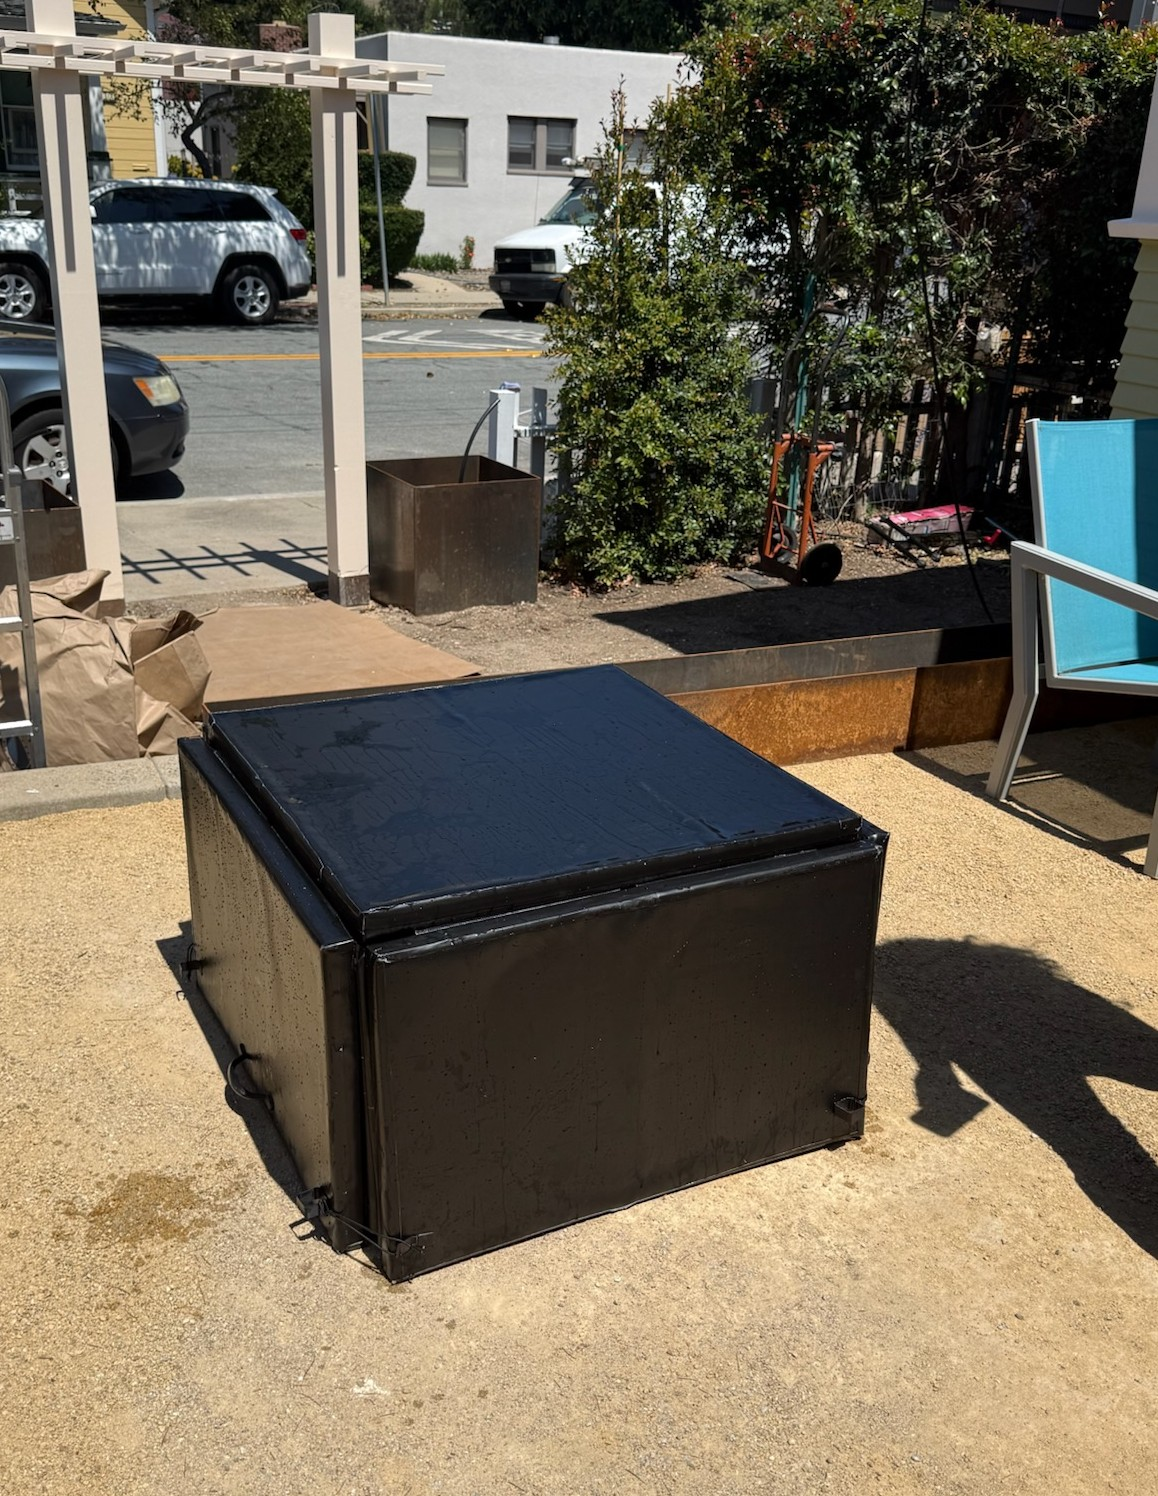
\includegraphics[
        width=1.58in,
        height=1.28in,
        keepaspectratio
    ]{foam_model_folded_backyard_image}
};
\end{scope}

\draw[RuleGray,line width=0.55pt,rounded corners=4pt]
    ($(current page.north west)+(9.19in,-5.04in)$)
    rectangle
    ($(current page.north east)+(-0.43in,-6.43in)$);

% Larger captions
\node[anchor=north,align=center,text width=1.95in,text=Muted,
      font=\sffamily\fontsize{6.8}{7.4}\selectfont]
at ($(current page.north west)+(1.47in,-6.49in)$)
{Topside panel architecture};

\node[anchor=north,align=center,text width=1.95in,text=Muted,
      font=\sffamily\fontsize{6.8}{7.4}\selectfont]
at ($(current page.north west)+(3.66in,-6.49in)$)
{Underside hinge architecture};

\node[anchor=north,align=center,text width=1.95in,text=Muted,
      font=\sffamily\fontsize{6.8}{7.4}\selectfont]
at ($(current page.north west)+(5.85in,-6.49in)$)
{Folded CAD configuration};

\node[anchor=north,align=center,text width=1.95in,text=Muted,
      font=\sffamily\fontsize{6.8}{7.4}\selectfont]
at ($(current page.north west)+(8.04in,-6.49in)$)
{Dual-use product vision};

\node[anchor=north,align=center,text width=1.95in,text=Muted,
      font=\sffamily\fontsize{6.8}{7.4}\selectfont]
at ($(current page.north west)+(9.88in,-6.49in)$)
{Folded foam prototype};

% Page 1 resource bar — centered and non-repeated resources
\fill[Panel,rounded corners=4pt]
    ($(current page.north west)+(0.43in,-7.05in)$)
    rectangle
    ($(current page.north east)+(-0.43in,-7.64in)$);
\draw[RuleGray,line width=0.5pt,rounded corners=4pt]
    ($(current page.north west)+(0.43in,-7.05in)$)
    rectangle
    ($(current page.north east)+(-0.43in,-7.64in)$);

\node[
    anchor=center,
    align=center,
    text=DeepGreen,
    font=\sffamily\bfseries\fontsize{6.9}{7.5}\selectfont
]
at ($(current page.north)+(0,-7.345in)$)
{\href{\ToroDrawingLink}{\faDraftingCompass\ DRAWING PACKAGE}
\hspace{24pt}
\href{\ToroDimensionsLink}{\faImage\ DIMENSION STUDY}
\hspace{24pt}
\href{\ToroProblemLink}{\faFileImage\ PROBLEM STATEMENT}};

% Footer
\node[
    anchor=south west,
    text=white,
    font=\sffamily\bfseries\fontsize{7.1}{7.7}\selectfont
]
at ($(current page.south west)+(0.42in,0.17in)$)
{\hyperlink{composites}{\faArrowLeft\ COMPOSITES}};

\node[
    anchor=south,
    text=white,
    font=\sffamily\fontsize{7.0}{7.6}\selectfont
]
at ($(current page.south)+(0,0.17in)$)
{TORO COVER \hspace{6pt} 1 / 3};

\node[
    anchor=south east,
    text=white,
    font=\sffamily\bfseries\fontsize{7.1}{7.7}\selectfont
]
at ($(current page.south east)+(-0.42in,0.17in)$)
{MANUFACTURING-DRIVEN DESIGN \faArrowRight};

\end{tikzpicture}


% ============================================================
% PAGE 2 — MANUFACTURING-DRIVEN DESIGN
% ============================================================

\clearpage
\thispagestyle{empty}
\hypertarget{toro-manufacturing}{}
\null

\begin{tikzpicture}[remember picture,overlay]

% Background and bars
\fill[white]
    (current page.south west)
    rectangle
    (current page.north east);

\fill[DeepGreen]
    (current page.north west)
    rectangle
    ($(current page.north east)+(0,-0.095in)$);

\fill[PolyGold]
    ($(current page.north west)+(0,-0.095in)$)
    rectangle
    ($(current page.north east)+(0,-0.14in)$);

\fill[DeepGreen]
    (current page.south west)
    rectangle
    ($(current page.south east)+(0,0.36in)$);

\fill[PolyGold]
    ($(current page.south west)+(0,0.36in)$)
    rectangle
    ($(current page.south east)+(0,0.405in)$);

% Header
\node[
    anchor=north west,
    text=PolyGold,
    font=\sffamily\bfseries\fontsize{8.1}{8.7}\selectfont
]
at ($(current page.north west)+(0.42in,-0.39in)$)
{TORO COVER \hspace{5pt}/\hspace{5pt} DESIGN FOR MANUFACTURABILITY};

\node[
    anchor=north west,
    text=DeepGreen,
    font=\bfseries\fontsize{23}{24}\selectfont
]
at ($(current page.north west)+(0.40in,-0.67in)$)
{THE ENVELOPE METHOD};

\node[
    anchor=north west,
    text=Muted,
    font=\sffamily\fontsize{8.7}{9.6}\selectfont
]
at ($(current page.north west)+(0.42in,-1.12in)$)
{A one-layup process developed for unusually thick insulated composite sandwich panels};

\fill[PolyGold]
    ($(current page.north west)+(0.42in,-1.36in)$)
    rectangle
    ($(current page.north west)+(5.30in,-1.315in)$);

% Process explanation
\fill[SoftGold,rounded corners=5pt]
    ($(current page.north west)+(0.42in,-1.61in)$)
    rectangle
    ($(current page.north east)+(-0.42in,-2.90in)$);

\fill[PolyGold]
    ($(current page.north west)+(0.42in,-1.61in)$)
    rectangle
    ($(current page.north west)+(0.52in,-2.90in)$);

\node[
    anchor=north west,
    text=DeepGreen,
    font=\sffamily\bfseries\fontsize{7.9}{8.6}\selectfont
]
at ($(current page.north west)+(0.67in,-1.76in)$)
{PROCESS INNOVATION};

\node[
    anchor=north west,
    align=left,
    text width=9.55in,
    text=Ink,
    font=\fontsize{7.35}{8.75}\selectfont
]
at ($(current page.north west)+(0.67in,-2.02in)$)
{
Weight reduction and insulation were both essential, leading to the selection of an
XPS foam core. Because XPS could not tolerate composite heat-cure temperatures, prepreg
processing was not practical and the panels had to be manufactured by wet layup with a
room-temperature cure. To simplify this process, I waterjet-cut XPS perimeter strips from
excess foam and placed them around each core inside the vacuum enclosure. Under vacuum,
the top and bottom carbon skins met along the panel sides and compressed against this
border, eliminating a separate edge-banding layup and reducing corner pleating.
};

% Workflow title
\node[
    anchor=north west,
    text=DeepGreen,
    font=\sffamily\bfseries\fontsize{8.0}{8.7}\selectfont
]
at ($(current page.north west)+(0.43in,-3.06in)$)
{MANUFACTURING WORKFLOW};

% Row 1 image 1
\node[anchor=center,inner sep=0pt]
at ($(current page.north west)+(2.07in,-4.105in)$)
{
    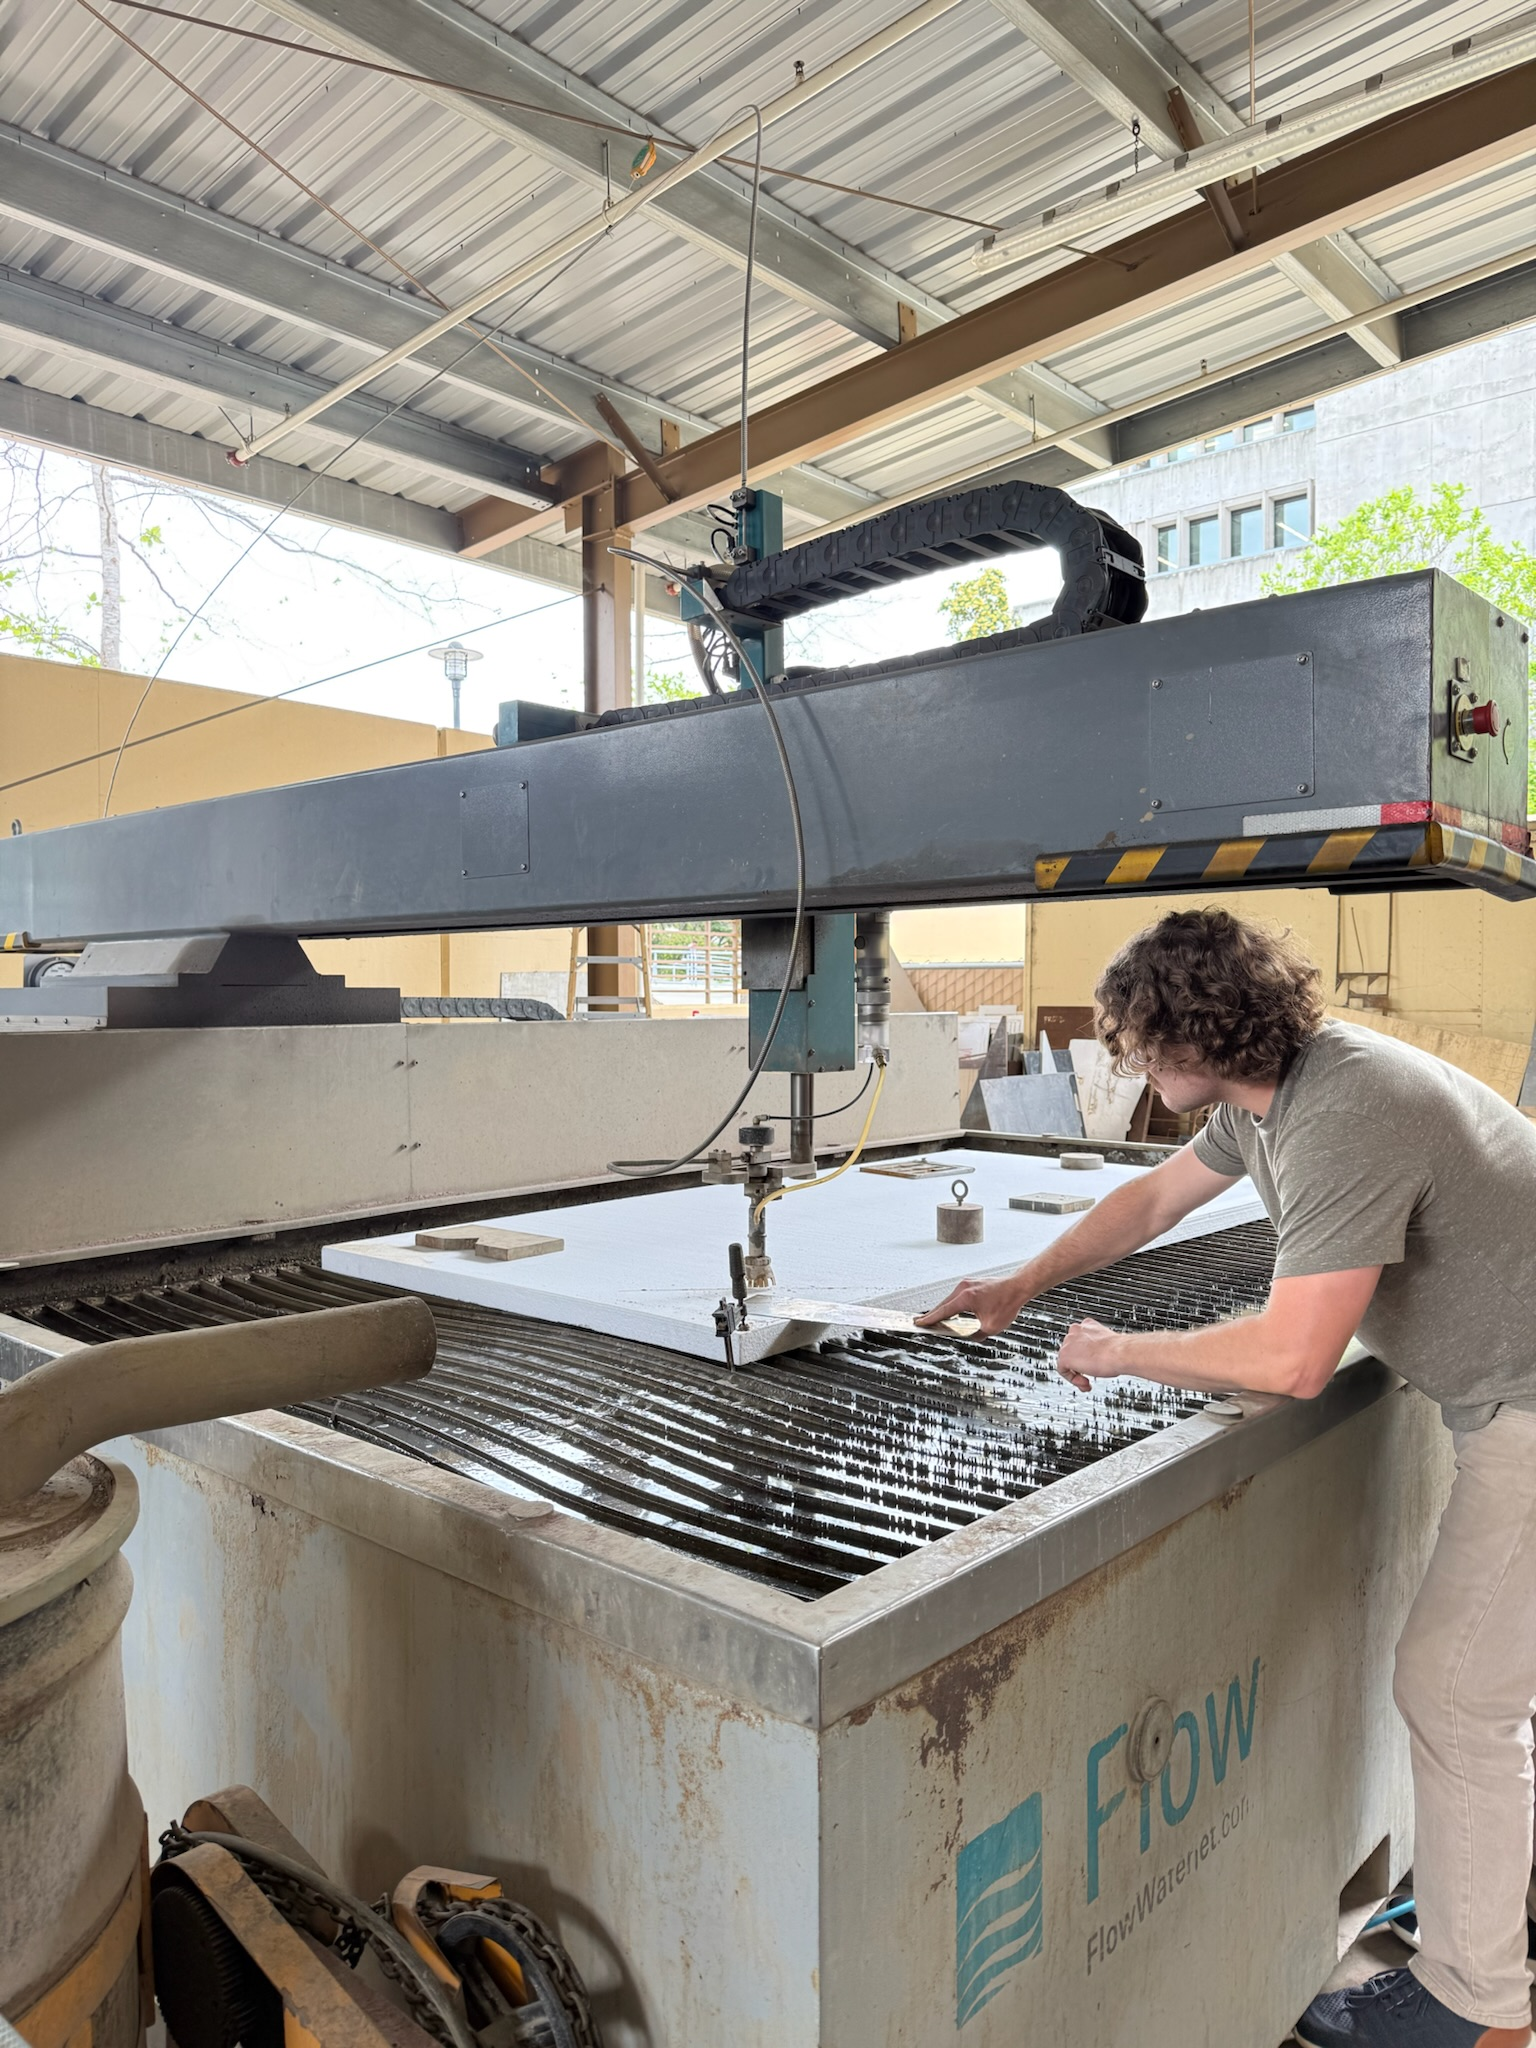
\includegraphics[
        width=3.10in,
        height=1.40in,
        keepaspectratio
    ]{waterjet_foam}
};
\draw[RuleGray,line width=0.55pt,rounded corners=4pt]
    ($(current page.north west)+(0.43in,-3.36in)$)
    rectangle
    ($(current page.north west)+(3.71in,-4.85in)$);

% Row 1 image 2
\node[anchor=center,inner sep=0pt]
at ($(current page.north west)+(5.50in,-4.105in)$)
{
    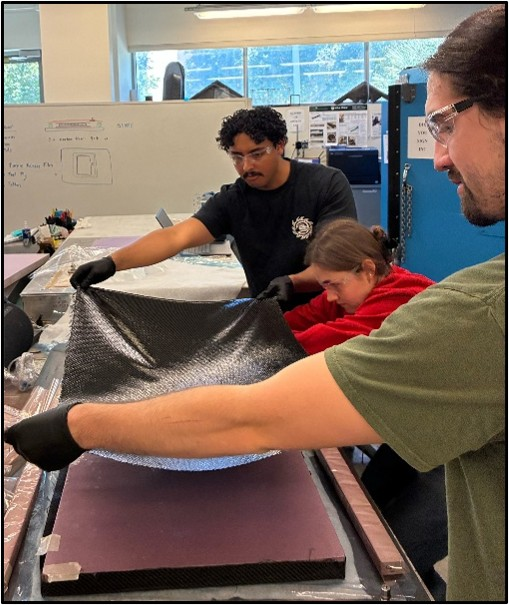
\includegraphics[
        width=3.10in,
        height=1.40in,
        keepaspectratio
    ]{group_layup}
};
\draw[RuleGray,line width=0.55pt,rounded corners=4pt]
    ($(current page.north west)+(3.86in,-3.36in)$)
    rectangle
    ($(current page.north west)+(7.14in,-4.85in)$);

% Row 1 image 3
\node[anchor=center,inner sep=0pt]
at ($(current page.north west)+(8.935in,-4.105in)$)
{
    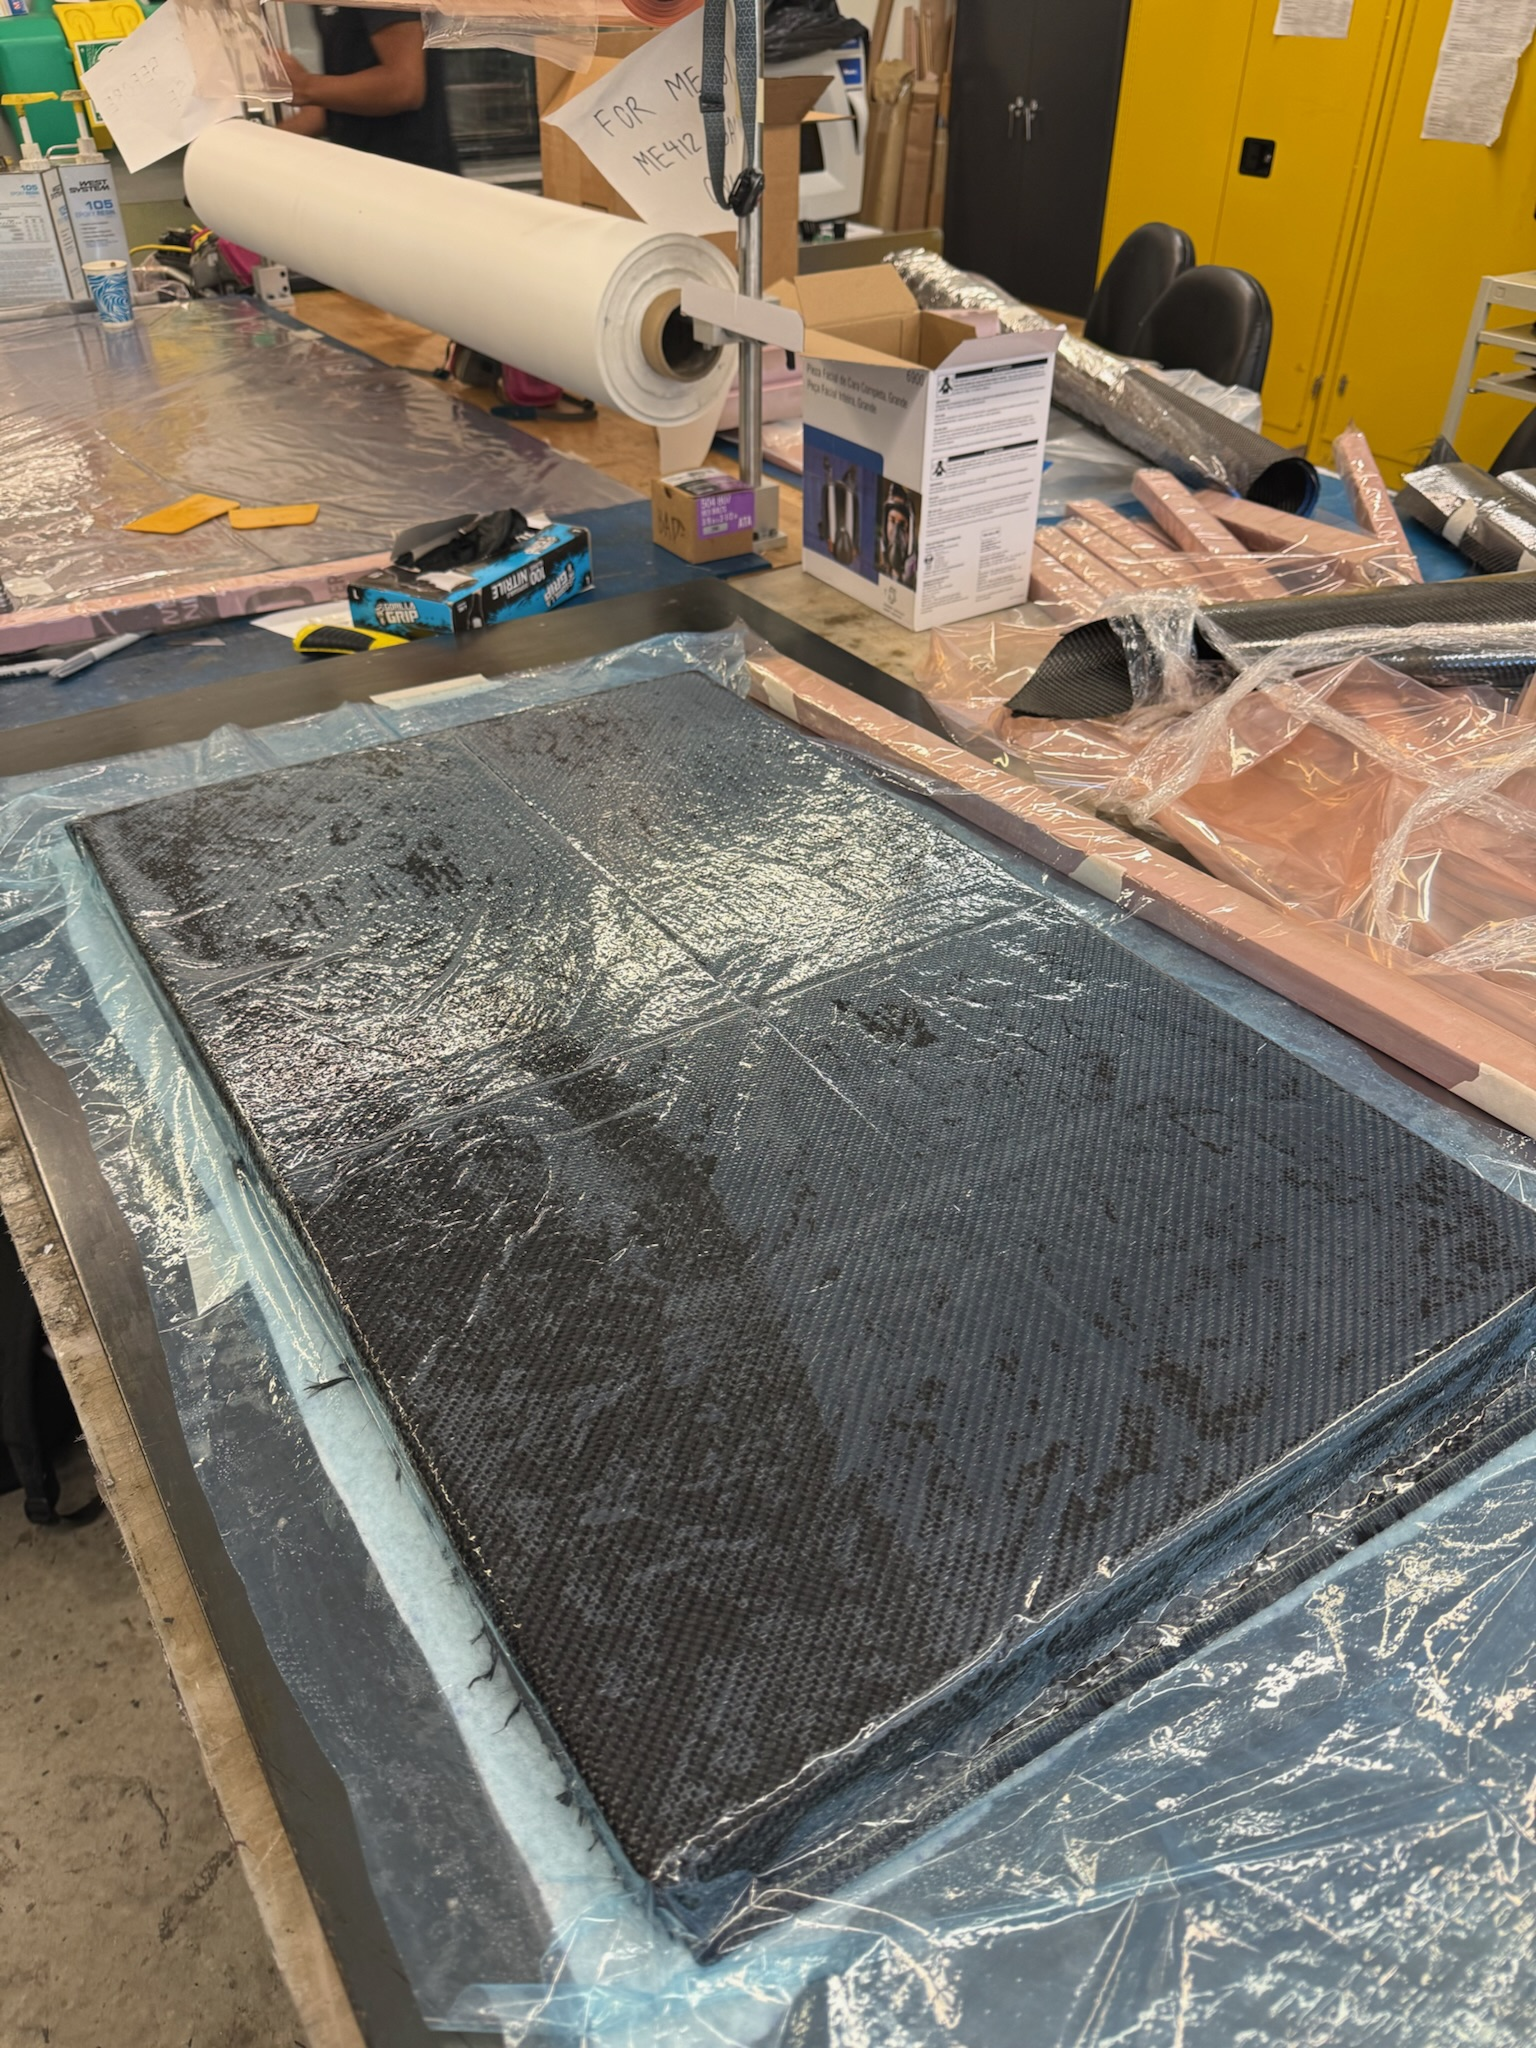
\includegraphics[
        width=3.10in,
        height=1.40in,
        keepaspectratio
    ]{blue_perforrated_film_layup}
};
\draw[RuleGray,line width=0.55pt,rounded corners=4pt]
    ($(current page.north west)+(7.29in,-3.36in)$)
    rectangle
    ($(current page.north east)+(-0.42in,-4.85in)$);

% Row 1 captions
\node[anchor=north,text=Muted,font=\sffamily\fontsize{6.7}{7.3}\selectfont]
at ($(current page.north west)+(2.07in,-4.90in)$)
{1. Waterjet-cut core and perimeter geometry};

\node[anchor=north,text=Muted,font=\sffamily\fontsize{6.7}{7.3}\selectfont]
at ($(current page.north west)+(5.50in,-4.90in)$)
{2. Team wet layup under my process guidance};

\node[anchor=north,text=Muted,font=\sffamily\fontsize{6.7}{7.3}\selectfont]
at ($(current page.north west)+(8.935in,-4.90in)$)
{3. Perforated film, breather, and vacuum enclosure};

% Row 2 image 1
\node[anchor=center,inner sep=0pt]
at ($(current page.north west)+(2.07in,-5.875in)$)
{
    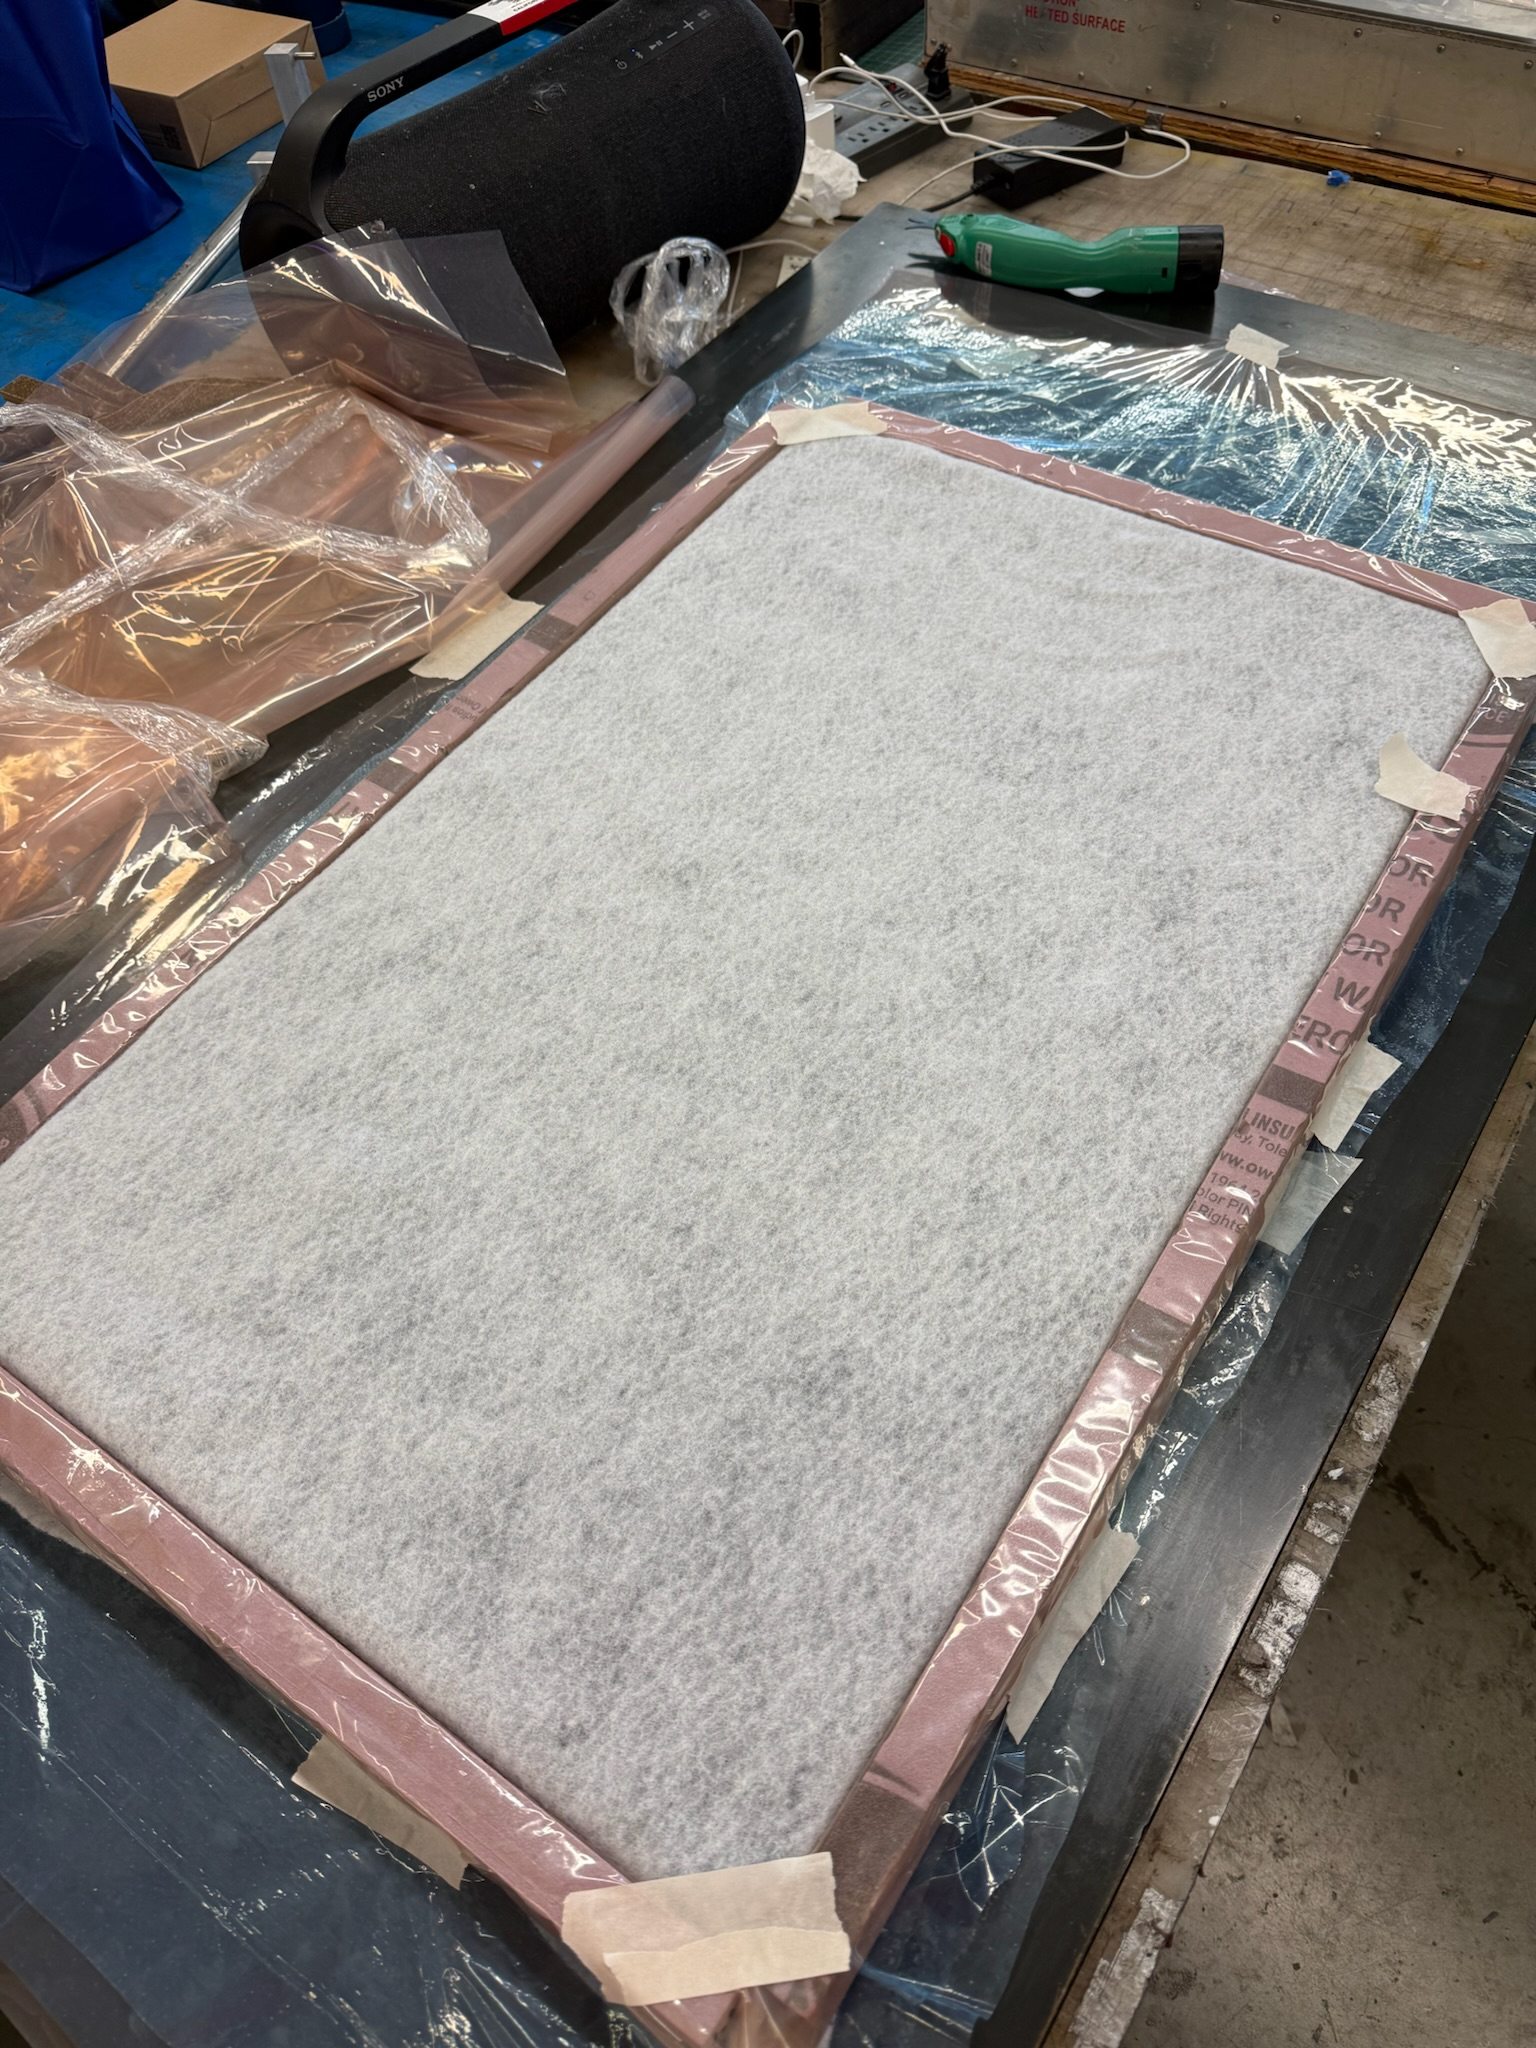
\includegraphics[
        width=3.10in,
        height=1.40in,
        keepaspectratio
    ]{completed_layup}
};
\draw[RuleGray,line width=0.55pt,rounded corners=4pt]
    ($(current page.north west)+(0.43in,-5.13in)$)
    rectangle
    ($(current page.north west)+(3.71in,-6.62in)$);

% Row 2 image 2 — oven chamber used only as a reliable vacuum enclosure; no heat applied
\node[anchor=center,inner sep=0pt]
at ($(current page.north west)+(5.50in,-5.875in)$)
{
    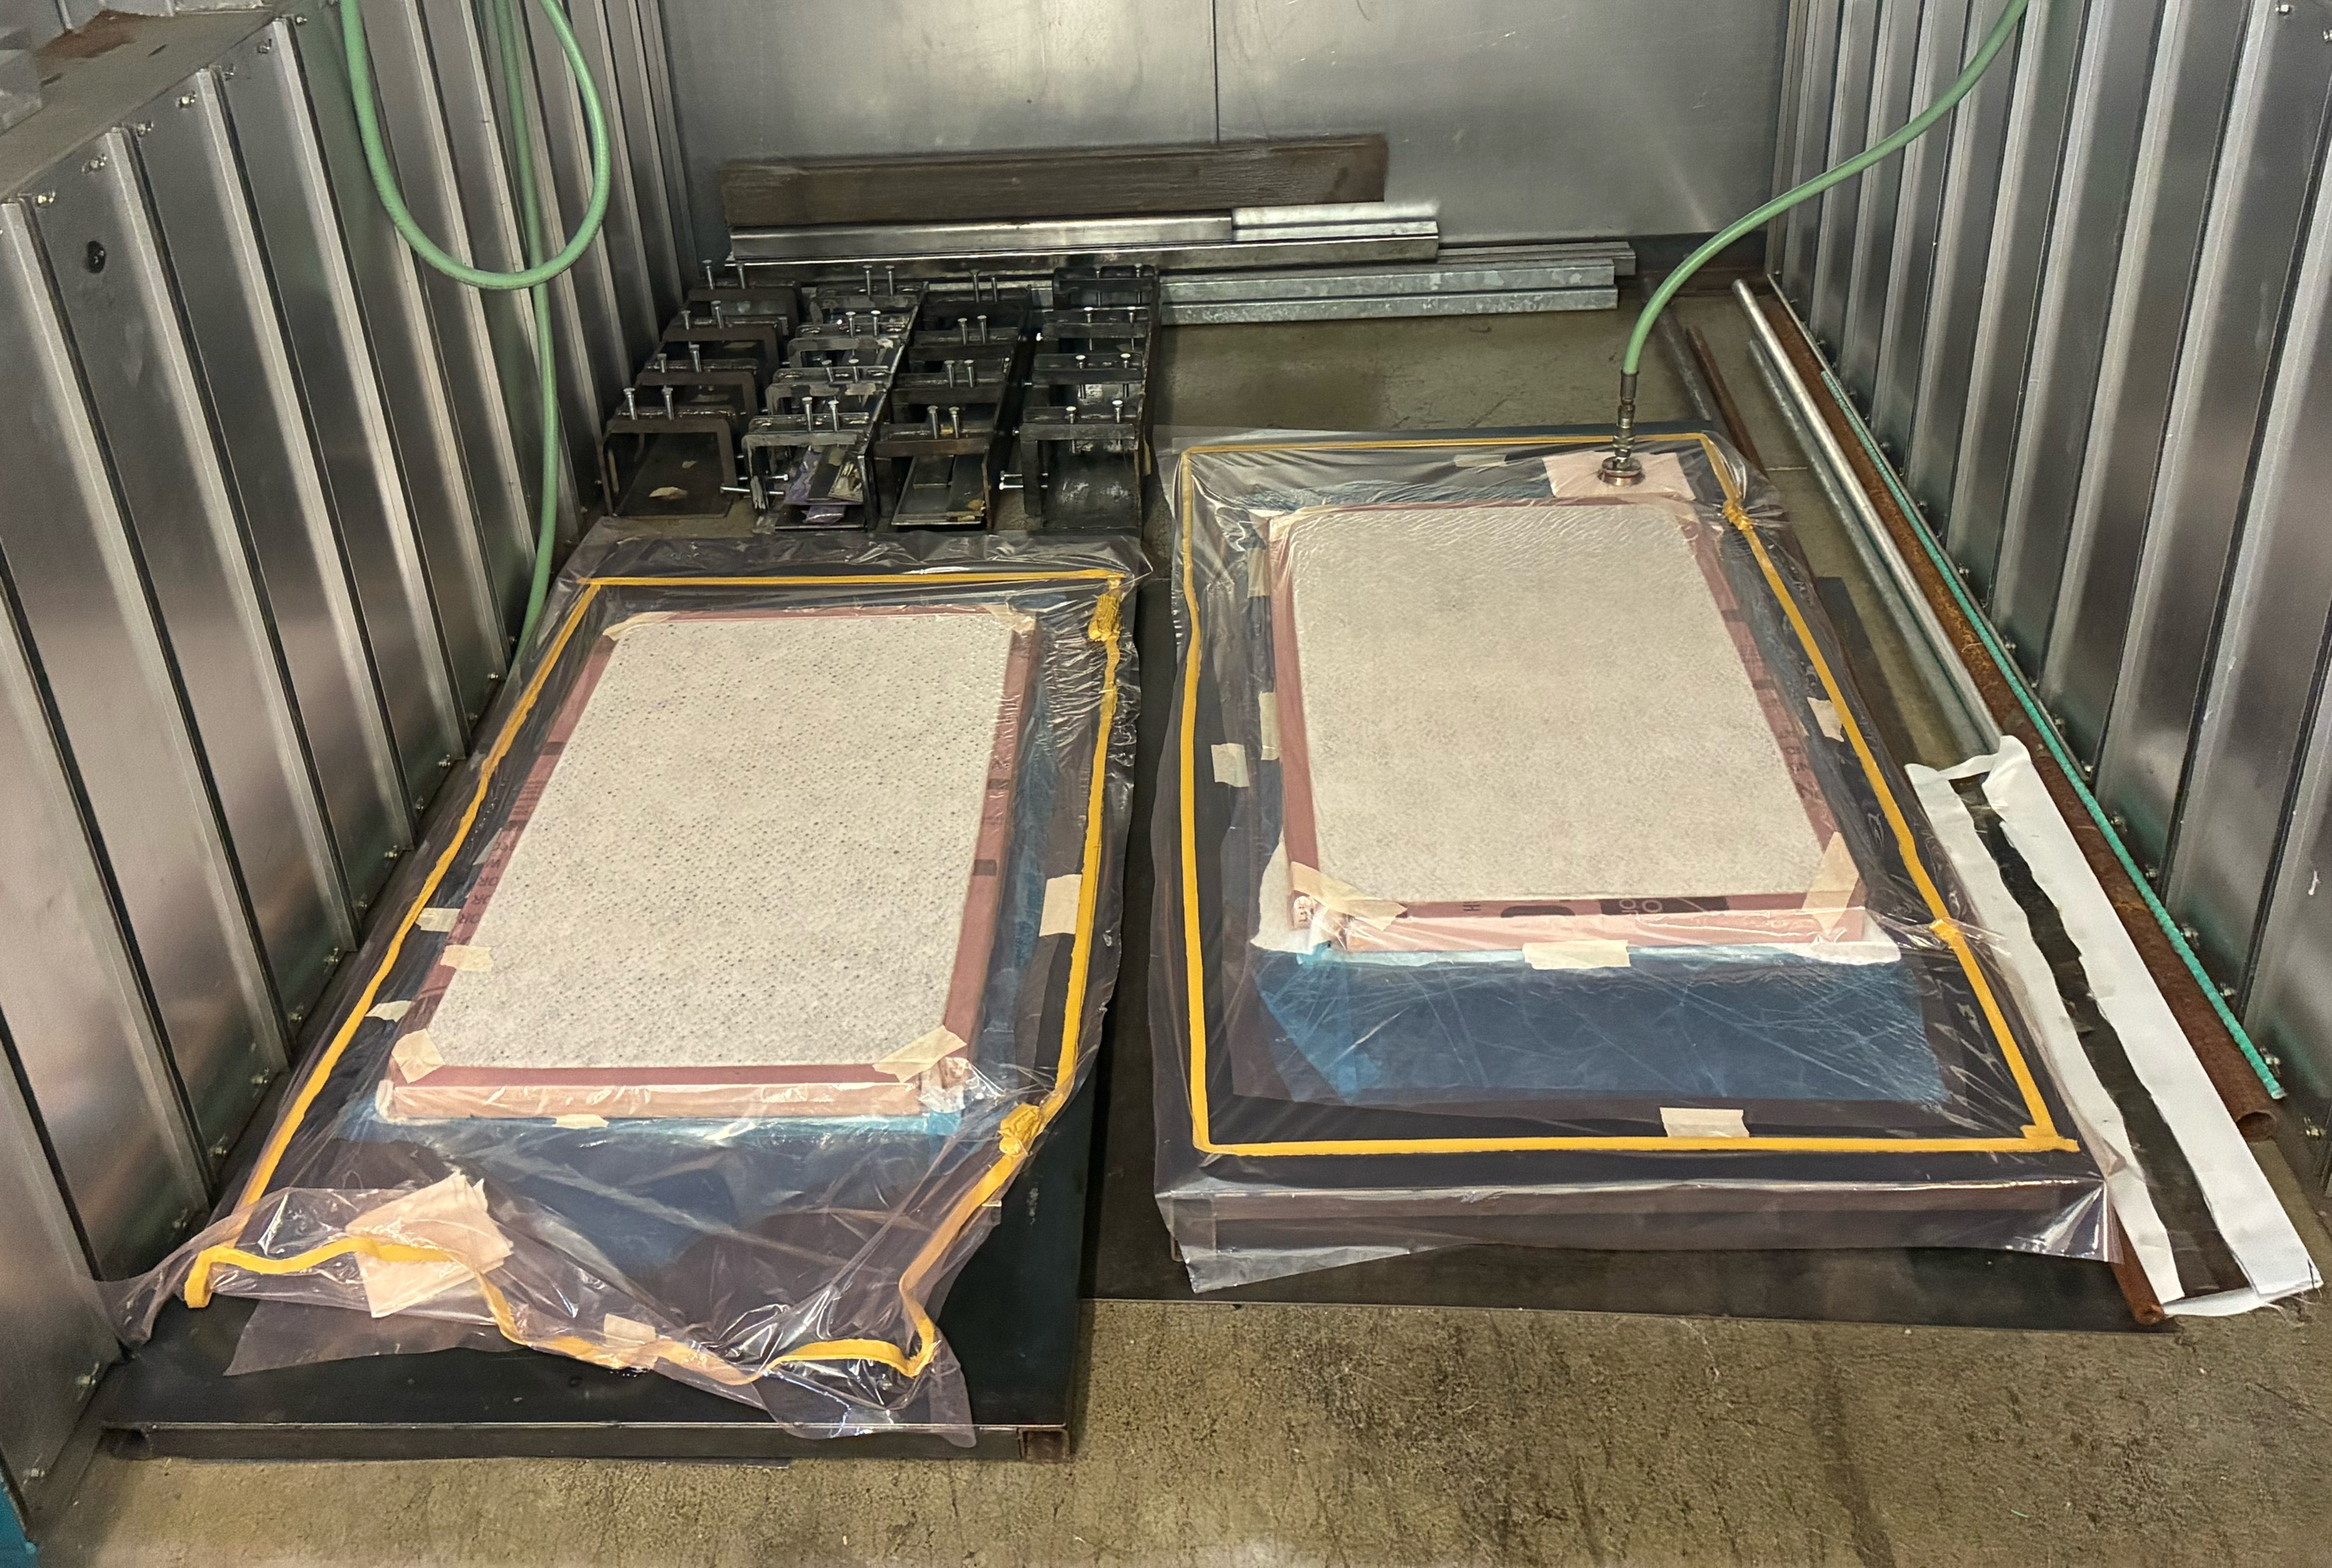
\includegraphics[
        width=3.10in,
        height=1.40in,
        keepaspectratio
    ]{layups_in_composite_oven_under_vacuumPressure}
};
\draw[RuleGray,line width=0.55pt,rounded corners=4pt]
    ($(current page.north west)+(3.86in,-5.13in)$)
    rectangle
    ($(current page.north west)+(7.14in,-6.62in)$);

% Row 2 image 3
\node[anchor=center,inner sep=0pt]
at ($(current page.north west)+(8.935in,-5.875in)$)
{
    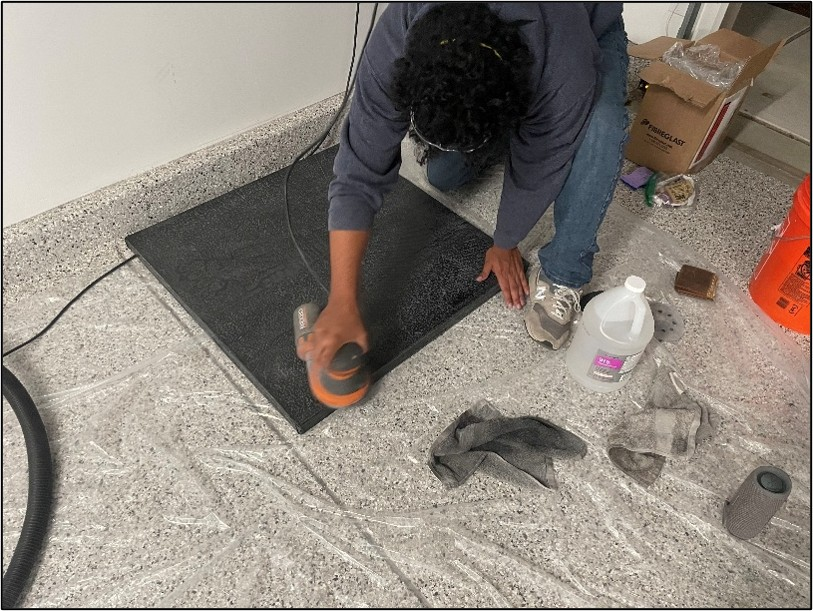
\includegraphics[
        width=3.10in,
        height=1.40in,
        keepaspectratio
    ]{garage_sanding}
};
\draw[RuleGray,line width=0.55pt,rounded corners=4pt]
    ($(current page.north west)+(7.29in,-5.13in)$)
    rectangle
    ($(current page.north east)+(-0.42in,-6.62in)$);

% Row 2 captions
\node[anchor=north,text=Muted,font=\sffamily\fontsize{6.7}{7.3}\selectfont]
at ($(current page.north west)+(2.07in,-6.67in)$)
{4. Fully saturated carbon skin and foam sandwich};

\node[anchor=north,text=Muted,font=\sffamily\fontsize{6.7}{7.3}\selectfont]
at ($(current page.north west)+(5.50in,-6.67in)$)
{5. Room-temperature cure under continuous vacuum};

\node[anchor=north,text=Muted,font=\sffamily\fontsize{6.7}{7.3}\selectfont]
at ($(current page.north west)+(8.935in,-6.67in)$)
{6. Post-processing and surface preparation};

% Bottom callouts
\fill[Panel,rounded corners=4pt]
    ($(current page.north west)+(0.43in,-6.95in)$)
    rectangle
    ($(current page.north west)+(5.48in,-7.60in)$);

\draw[RuleGray,line width=0.55pt,rounded corners=4pt]
    ($(current page.north west)+(0.43in,-6.95in)$)
    rectangle
    ($(current page.north west)+(5.48in,-7.60in)$);

\node[
    anchor=north west,
    text=DeepGreen,
    font=\sffamily\bfseries\fontsize{7.0}{7.6}\selectfont
]
at ($(current page.north west)+(0.63in,-7.08in)$)
{FROM THREE LAYUPS TO ONE};

\node[
    anchor=north west,
    align=left,
    text width=4.56in,
    text=Ink,
    font=\fontsize{6.45}{7.45}\selectfont
]
at ($(current page.north west)+(0.63in,-7.29in)$)
{
The Envelope Method reduced labor, cure cycles, handling,
alignment risk, and time spent forming numerous vacuum-bag
pleats around the 1.5-inch-thick XPS panels.
};

\fill[Panel,rounded corners=4pt]
    ($(current page.north west)+(5.68in,-6.95in)$)
    rectangle
    ($(current page.north east)+(-0.42in,-7.60in)$);

\draw[RuleGray,line width=0.55pt,rounded corners=4pt]
    ($(current page.north west)+(5.68in,-6.95in)$)
    rectangle
    ($(current page.north east)+(-0.42in,-7.60in)$);

\node[
    anchor=north west,
    text=DeepGreen,
    font=\sffamily\bfseries\fontsize{7.0}{7.6}\selectfont
]
at ($(current page.north west)+(5.88in,-7.08in)$)
{WHY SURFACE-BONDED HARDWARE};

\node[
    anchor=north west,
    align=left,
    text width=4.55in,
    text=Ink,
    font=\fontsize{6.45}{7.45}\selectfont
]
at ($(current page.north west)+(5.88in,-7.29in)$)
{
Adhesively bonded hinges and fixtures preserved the clean
composite exterior and avoided drilled inserts, foam-core
crushing, added stress concentrations, and new leak paths.
};


% Footer
\node[
    anchor=south west,
    text=white,
    font=\sffamily\bfseries\fontsize{7.1}{7.7}\selectfont
]
at ($(current page.south west)+(0.42in,0.17in)$)
{\faArrowLeft\ PRODUCT ARCHITECTURE};

\node[
    anchor=south,
    text=white,
    font=\sffamily\fontsize{7.0}{7.6}\selectfont
]
at ($(current page.south)+(0,0.17in)$)
{TORO COVER \hspace{6pt} 2 / 3};

\node[
    anchor=south east,
    text=white,
    font=\sffamily\bfseries\fontsize{7.1}{7.7}\selectfont
]
at ($(current page.south east)+(-0.42in,0.17in)$)
{VALIDATION \& TAKEAWAYS \faArrowRight};

\end{tikzpicture}


% ============================================================
% PAGE 3 — FINISHING, VALIDATION, AND TAKEAWAYS
% ============================================================

\clearpage
\thispagestyle{empty}
\hypertarget{toro-results}{}
\null

\begin{tikzpicture}[remember picture,overlay]

% Background and bars
\fill[white]
    (current page.south west)
    rectangle
    (current page.north east);

\fill[DeepGreen]
    (current page.north west)
    rectangle
    ($(current page.north east)+(0,-0.095in)$);

\fill[PolyGold]
    ($(current page.north west)+(0,-0.095in)$)
    rectangle
    ($(current page.north east)+(0,-0.14in)$);

\fill[DeepGreen]
    (current page.south west)
    rectangle
    ($(current page.south east)+(0,0.36in)$);

\fill[PolyGold]
    ($(current page.south west)+(0,0.36in)$)
    rectangle
    ($(current page.south east)+(0,0.405in)$);

% Header
\node[
    anchor=north west,
    text=PolyGold,
    font=\sffamily\bfseries\fontsize{8.1}{8.7}\selectfont
]
at ($(current page.north west)+(0.42in,-0.39in)$)
{TORO COVER \hspace{5pt}/\hspace{5pt} VALIDATION AND ENGINEERING TAKEAWAYS};

\node[
    anchor=north west,
    text=DeepGreen,
    font=\bfseries\fontsize{22.5}{23.5}\selectfont
]
at ($(current page.north west)+(0.40in,-0.67in)$)
{FROM PROTOTYPE TO PRODUCT PATHWAY};

\node[
    anchor=north west,
    text=Muted,
    font=\sffamily\fontsize{8.7}{9.6}\selectfont
]
at ($(current page.north west)+(0.42in,-1.12in)$)
{Environmental protection, usability testing, scope decisions, and lessons from technical leadership};

\fill[PolyGold]
    ($(current page.north west)+(0.42in,-1.36in)$)
    rectangle
    ($(current page.north west)+(5.8in,-1.315in)$);

% Finishing title
\node[
    anchor=north west,
    text=DeepGreen,
    font=\sffamily\bfseries\fontsize{8.0}{8.7}\selectfont
]
at ($(current page.north west)+(0.43in,-1.62in)$)
{OUTDOOR FINISHING AND ENVIRONMENTAL PROTECTION};

% Image 1
\node[anchor=center,inner sep=0pt]
at ($(current page.north west)+(1.705in,-2.655in)$)
{
    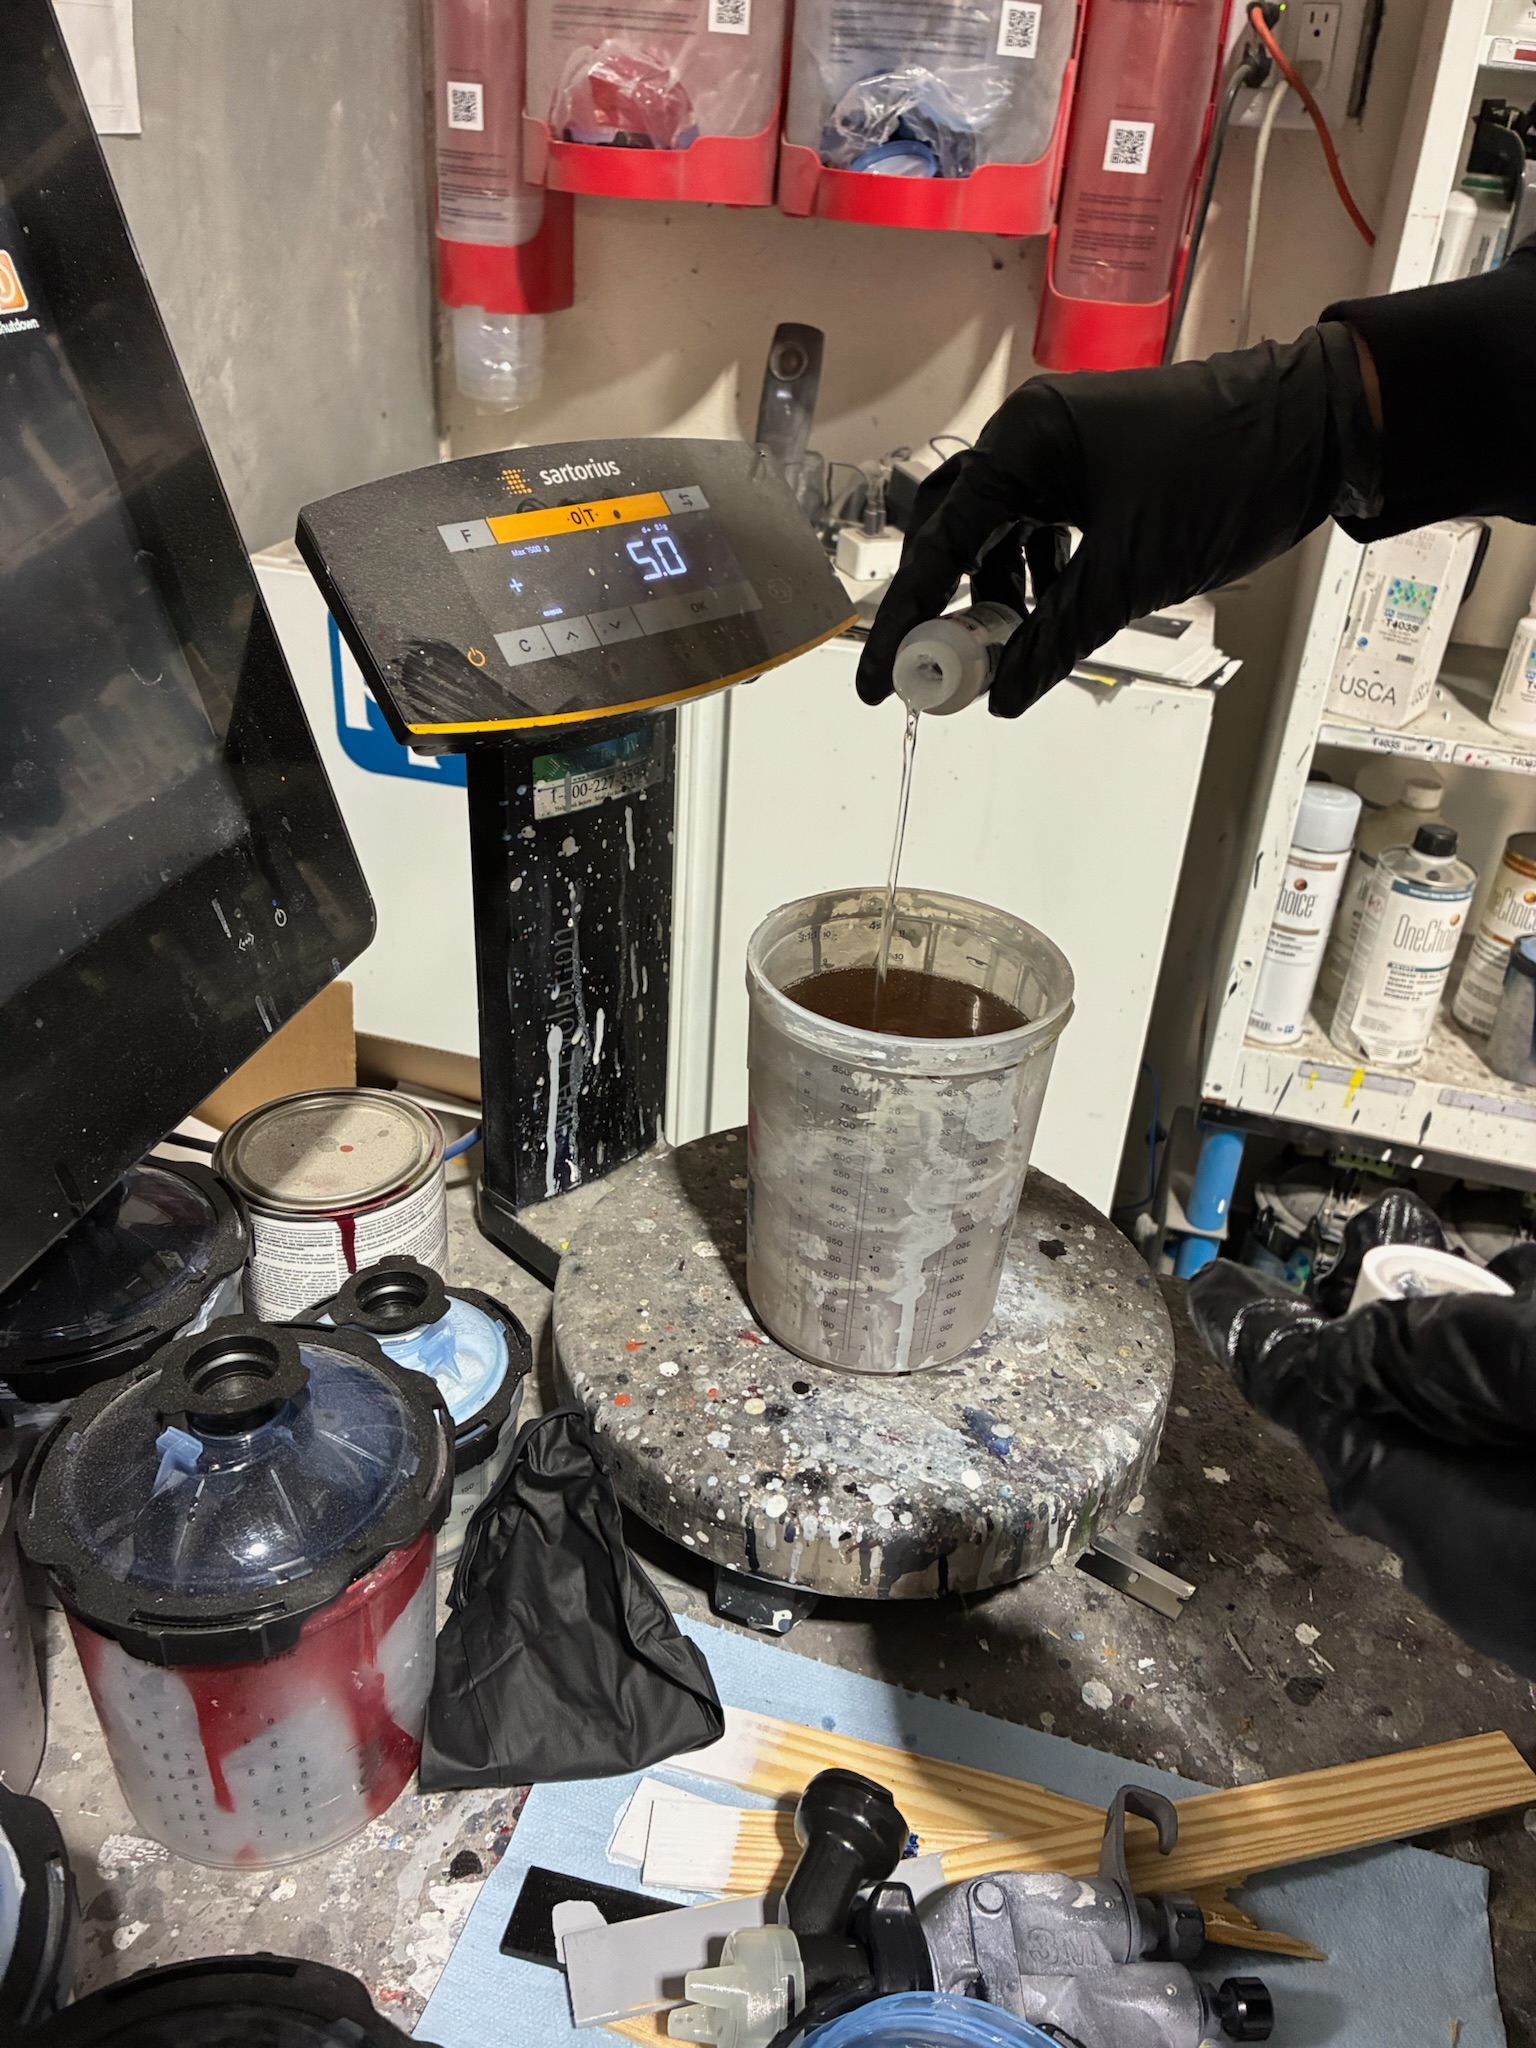
\includegraphics[
        width=2.35in,
        height=1.40in,
        keepaspectratio
    ]{spray_topcoat_prep}
};
\draw[RuleGray,line width=0.55pt,rounded corners=4pt]
    ($(current page.north west)+(0.43in,-1.91in)$)
    rectangle
    ($(current page.north west)+(2.98in,-3.40in)$);

% Image 2
\node[anchor=center,inner sep=0pt]
at ($(current page.north west)+(4.375in,-2.655in)$)
{
    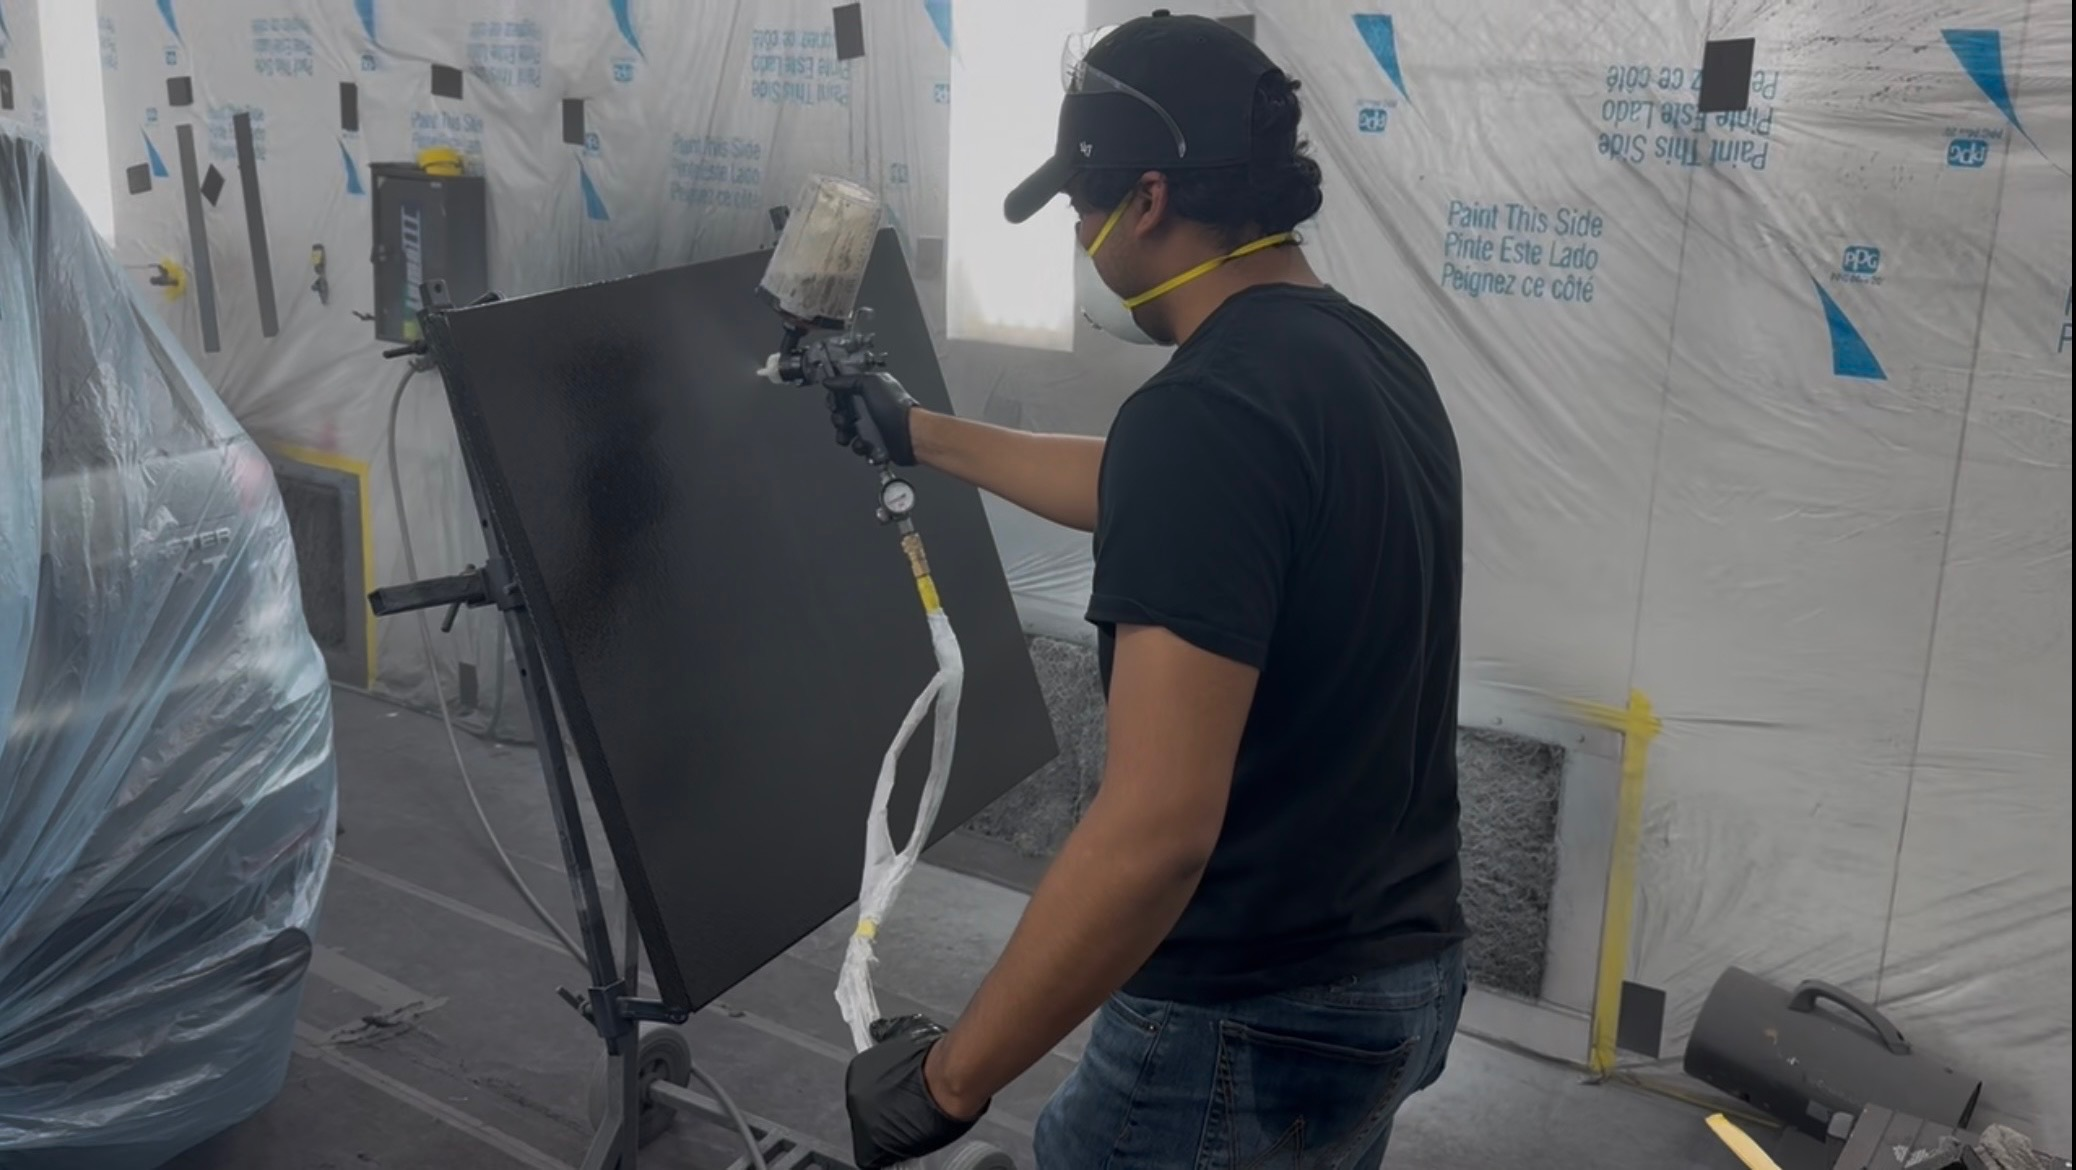
\includegraphics[
        width=2.35in,
        height=1.40in,
        keepaspectratio
    ]{spraying_topcoat}
};
\draw[RuleGray,line width=0.55pt,rounded corners=4pt]
    ($(current page.north west)+(3.10in,-1.91in)$)
    rectangle
    ($(current page.north west)+(5.65in,-3.40in)$);

% Image 3
\node[anchor=center,inner sep=0pt]
at ($(current page.north west)+(7.045in,-2.655in)$)
{
    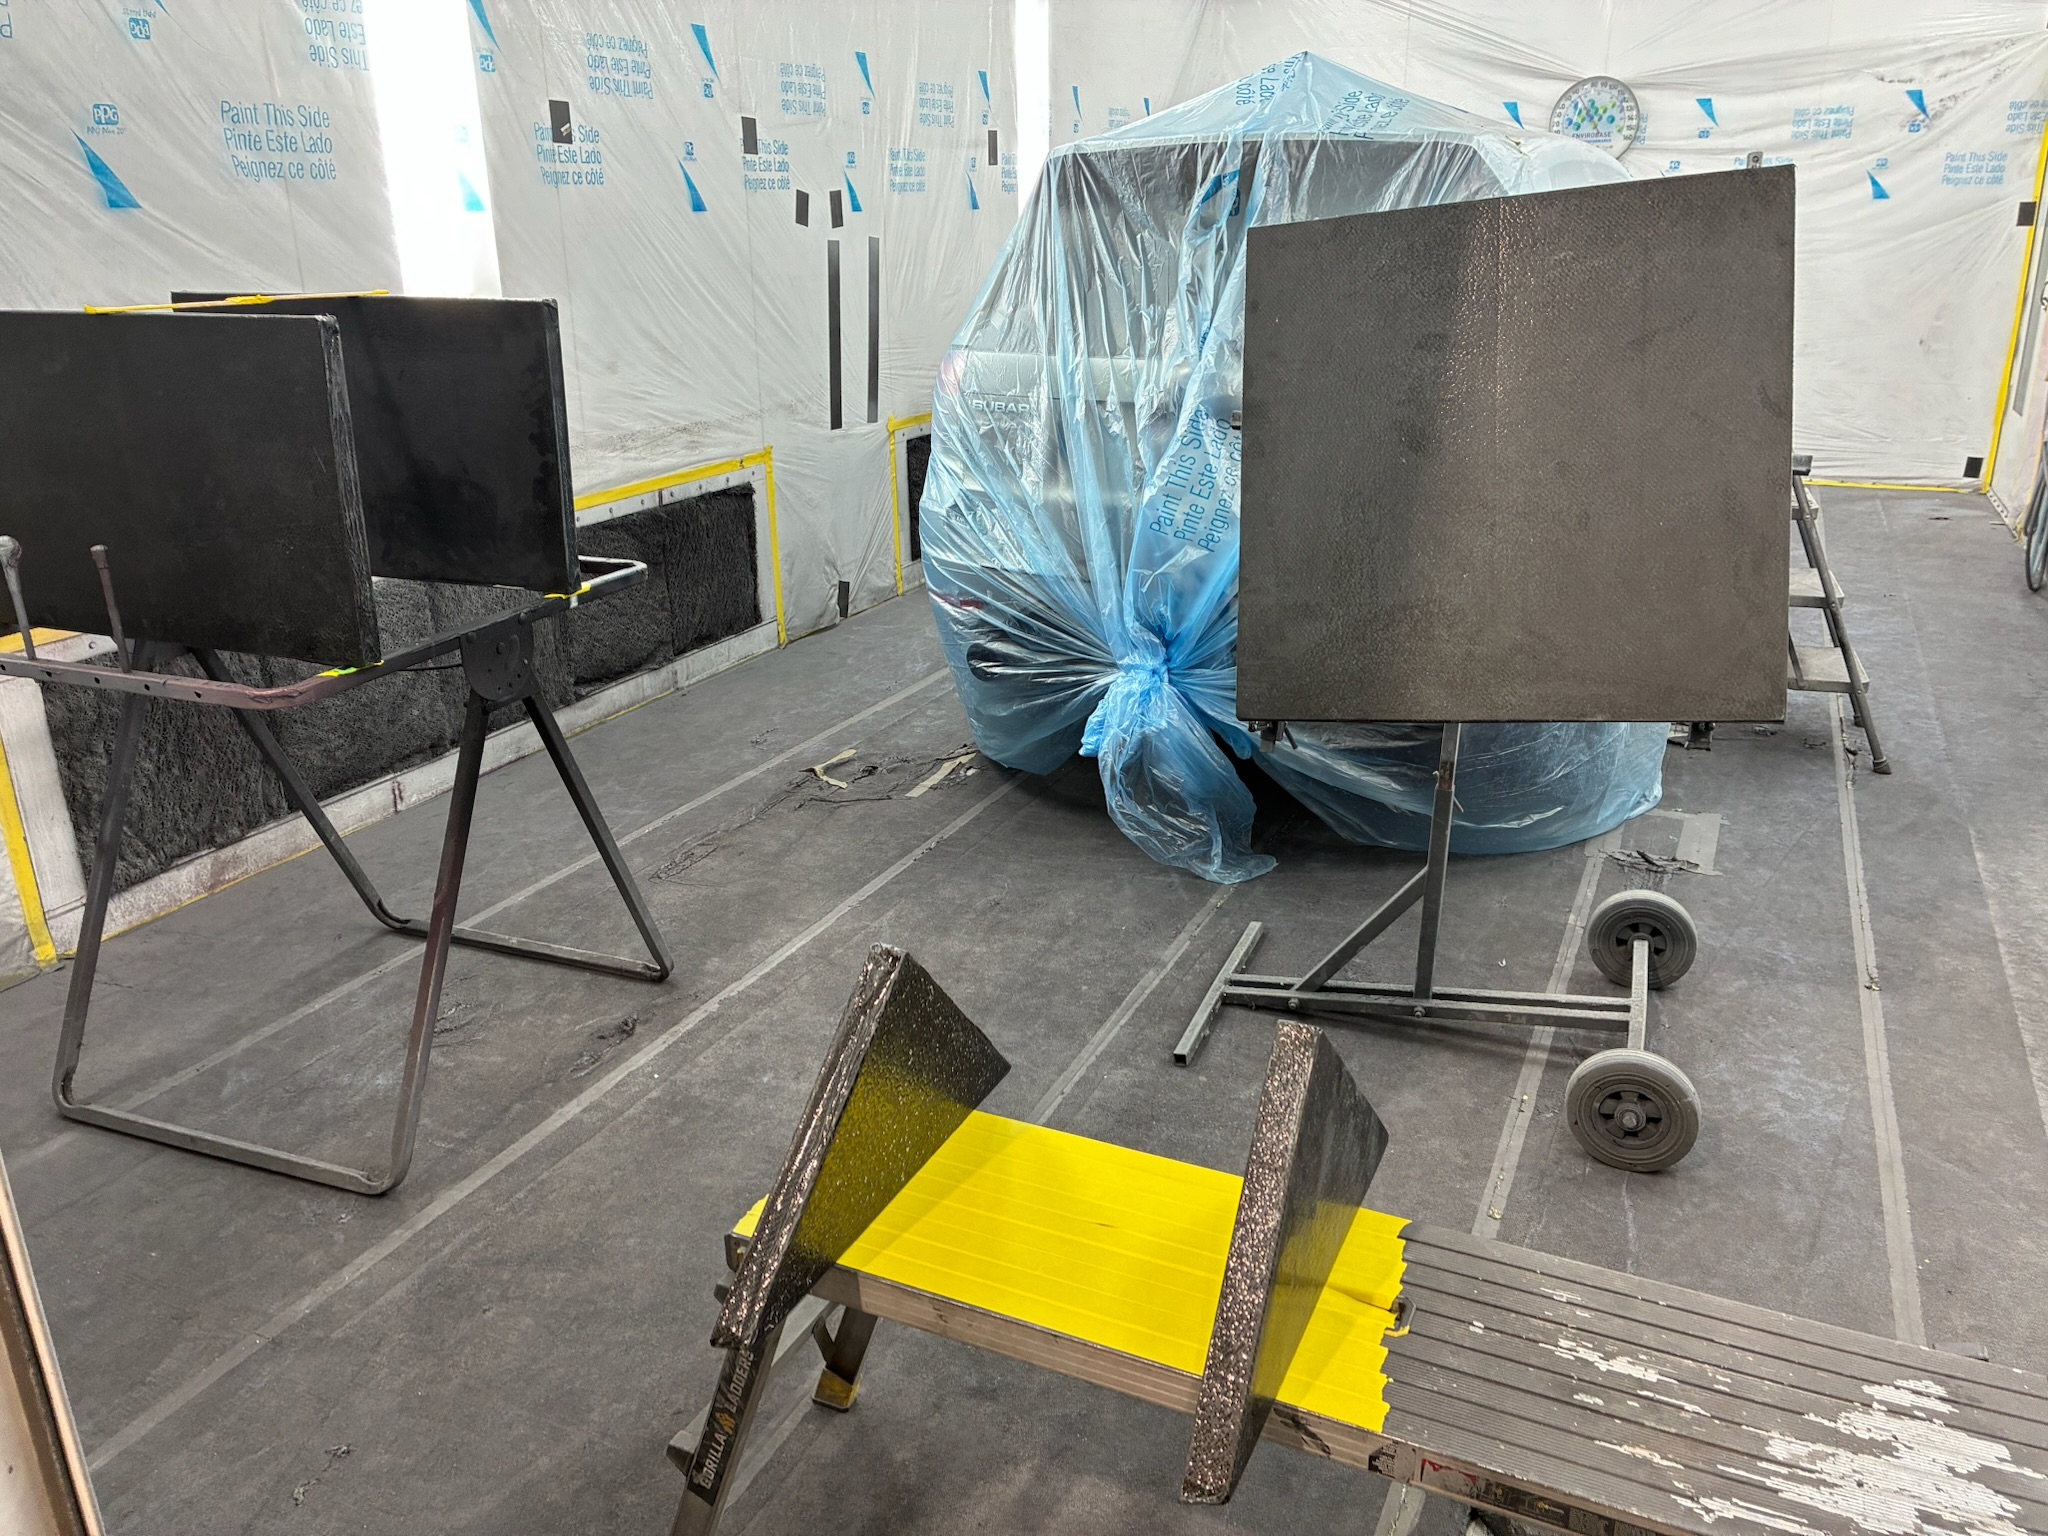
\includegraphics[
        width=2.35in,
        height=1.40in,
        keepaspectratio
    ]{topcoat_setup_apparatus}
};
\draw[RuleGray,line width=0.55pt,rounded corners=4pt]
    ($(current page.north west)+(5.77in,-1.91in)$)
    rectangle
    ($(current page.north west)+(8.32in,-3.40in)$);

% Image 4
\node[anchor=center,inner sep=0pt]
at ($(current page.north west)+(9.50in,-2.655in)$)
{
    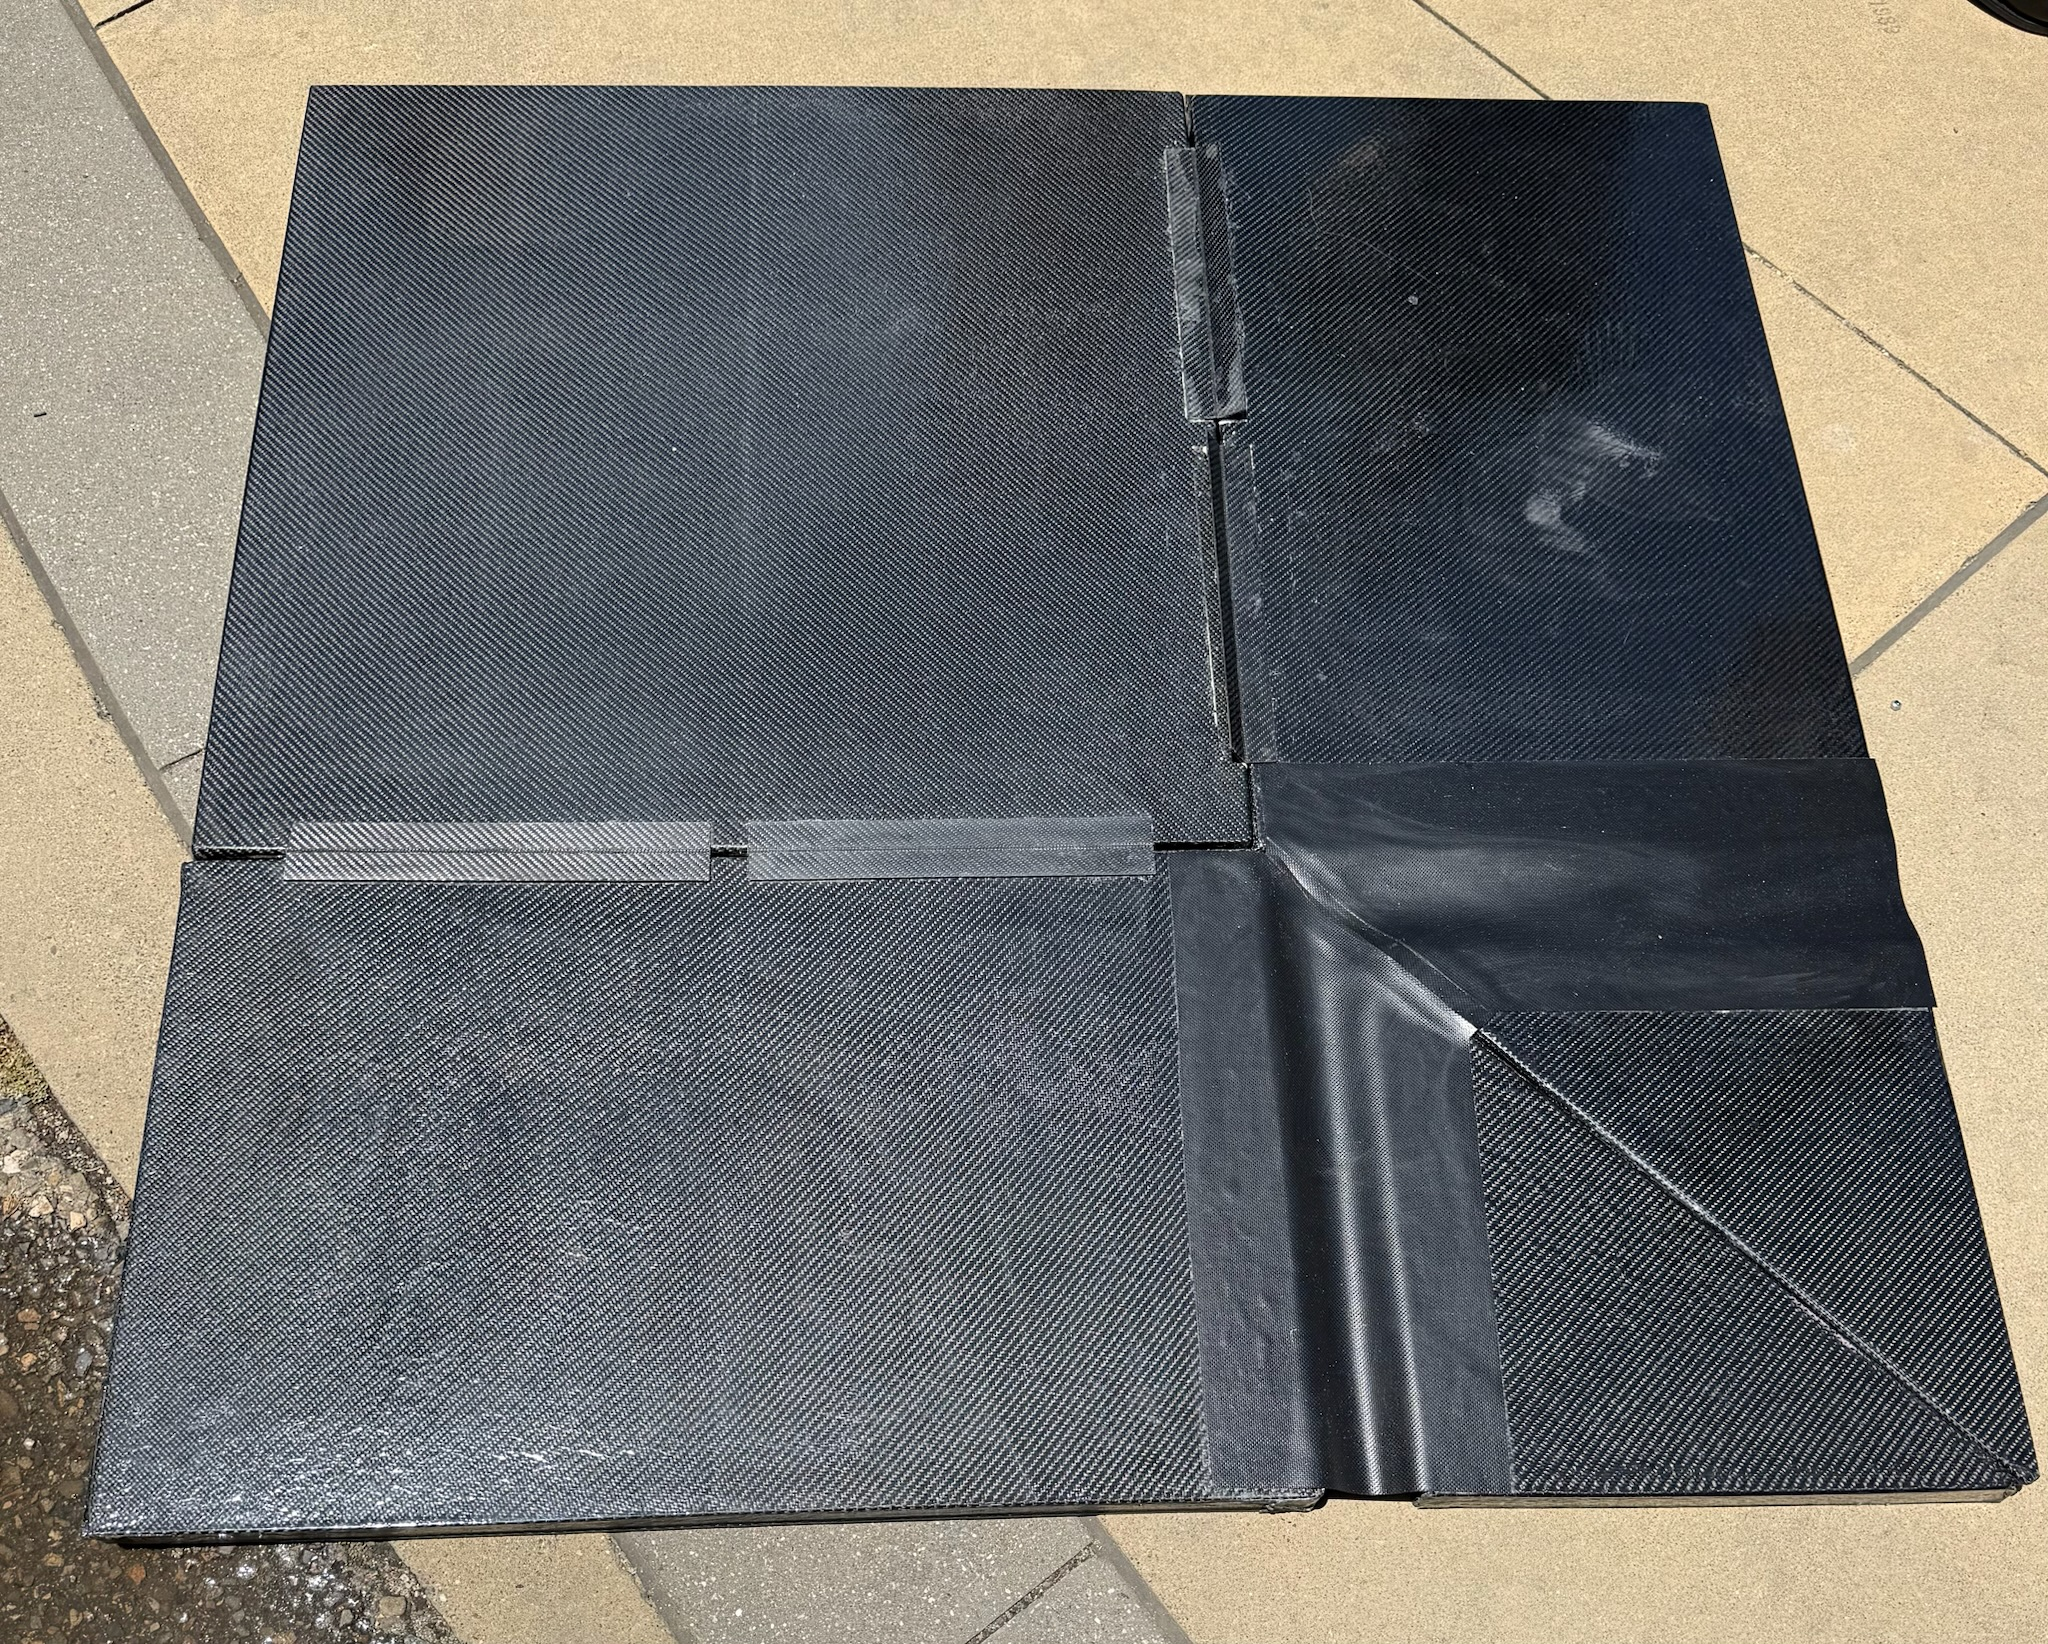
\includegraphics[
        width=2.35in,
        height=1.40in,
        keepaspectratio
    ]{refined_final_toro_cover_partial_carbon_model}
};
\draw[RuleGray,line width=0.55pt,rounded corners=4pt]
    ($(current page.north west)+(8.44in,-1.91in)$)
    rectangle
    ($(current page.north east)+(-0.42in,-3.40in)$);

% Captions
\node[anchor=north,text=Muted,font=\sffamily\fontsize{6.7}{7.3}\selectfont]
at ($(current page.north west)+(1.705in,-3.45in)$)
{Topcoat material preparation};

\node[anchor=north,text=Muted,font=\sffamily\fontsize{6.7}{7.3}\selectfont]
at ($(current page.north west)+(4.375in,-3.45in)$)
{Automotive-booth topcoat application};

\node[anchor=north,text=Muted,font=\sffamily\fontsize{6.7}{7.3}\selectfont]
at ($(current page.north west)+(7.045in,-3.45in)$)
{Coated panels drying after application};

\node[anchor=north,text=Muted,font=\sffamily\fontsize{6.7}{7.3}\selectfont]
at ($(current page.north west)+(9.50in,-3.45in)$)
{Partial carbon manufacturing model};

% Environmental rationale
\fill[SoftGold,rounded corners=4pt]
    ($(current page.north west)+(0.43in,-3.73in)$)
    rectangle
    ($(current page.north east)+(-0.42in,-4.76in)$);

\node[
    anchor=north west,
    align=left,
    text width=9.75in,
    text=Ink,
    font=\fontsize{7.05}{8.25}\selectfont
]
at ($(current page.north west)+(0.65in,-3.89in)$)
{
Because the sponsor required a carbon-fiber cover for outdoor use near chlorinated water,
environmental protection became a functional requirement rather than a cosmetic finish.
I selected and personally sprayed a UV-resistant Sunshield topcoat to seal minor laminate
porosity, reduce moisture ingress, preserve the carbon appearance, limit UV degradation of
the epoxy matrix, and isolate the composite surface from nearby metallic hardware.
};

% Results title
\node[
    anchor=north west,
    text=DeepGreen,
    font=\sffamily\bfseries\fontsize{8.0}{8.7}\selectfont
]
at ($(current page.north west)+(0.43in,-4.94in)$)
{FUNCTIONAL PROTOTYPE RESULTS};

% ------------------------------------------------------------
% Matched lower panels — larger type and improved allocation
% ------------------------------------------------------------

% Left results panel
\fill[SoftGreen,rounded corners=5pt]
    ($(current page.north west)+(0.43in,-5.22in)$)
    rectangle
    ($(current page.north west)+(5.98in,-7.39in)$);

\draw[RuleGray,line width=0.65pt,rounded corners=5pt]
    ($(current page.north west)+(0.43in,-5.22in)$)
    rectangle
    ($(current page.north west)+(5.98in,-7.39in)$);

\fill[DeepGreen,rounded corners=5pt]
    ($(current page.north west)+(0.43in,-5.22in)$)
    rectangle
    ($(current page.north west)+(5.98in,-5.58in)$);

\fill[DeepGreen]
    ($(current page.north west)+(0.43in,-5.40in)$)
    rectangle
    ($(current page.north west)+(5.98in,-5.58in)$);

\node[anchor=west,text=white,
      font=\sffamily\bfseries\fontsize{7.0}{7.6}\selectfont]
at ($(current page.north west)+(0.66in,-5.40in)$)
{SPECIFICATION};

\node[anchor=west,text=white,
      font=\sffamily\bfseries\fontsize{7.0}{7.6}\selectfont]
at ($(current page.north west)+(3.02in,-5.40in)$)
{RESULT};

\node[anchor=east,text=white,
      font=\sffamily\bfseries\fontsize{7.0}{7.6}\selectfont]
at ($(current page.north west)+(5.55in,-5.40in)$)
{STATUS};

\node[
    anchor=north west,
    align=left,
    text width=2.15in,
    text=Ink,
    font=\bfseries\fontsize{7.15}{8.55}\selectfont
]
at ($(current page.north west)+(0.66in,-5.72in)$)
{
Deployment time\\[3.4pt]
Removal time\\[3.4pt]
Single-user operation\\[3.4pt]
Single-side operation\\[3.4pt]
Deployment steps\\[3.4pt]
Removal steps\\[3.4pt]
Weight\\[3.4pt]
Folded storage
};

\node[
    anchor=north west,
    align=left,
    text width=1.45in,
    text=Ink,
    font=\fontsize{7.15}{8.55}\selectfont
]
at ($(current page.north west)+(3.02in,-5.72in)$)
{
25.51 seconds\\[3.4pt]
37.22 seconds\\[3.4pt]
100\% successful\\[3.4pt]
75\% successful\\[3.4pt]
6.4 average\\[3.4pt]
9 average\\[3.4pt]
17 lb\\[3.4pt]
2.9' x 2.9' x 1.7'
};

\node[
    anchor=north east,
    align=right,
    text width=1.05in,
    text=DeepGreen,
    font=\sffamily\bfseries\fontsize{7.05}{8.55}\selectfont
]
at ($(current page.north west)+(5.55in,-5.72in)$)
{
PASS\\[3.4pt]
PASS\\[3.4pt]
PASS\\[3.4pt]
NEAR TARGET\\[3.4pt]
PASS\\[3.4pt]
PASS\\[3.4pt]
NEAR TARGET\\[3.4pt]
PASS
};

% Right takeaways panel — widened for easier reading
\fill[SoftGreen,rounded corners=5pt]
    ($(current page.north west)+(6.14in,-5.22in)$)
    rectangle
    ($(current page.north east)+(-0.42in,-7.39in)$);

\draw[RuleGray,line width=0.65pt,rounded corners=5pt]
    ($(current page.north west)+(6.14in,-5.22in)$)
    rectangle
    ($(current page.north east)+(-0.42in,-7.39in)$);

\fill[DeepGreen,rounded corners=5pt]
    ($(current page.north west)+(6.14in,-5.22in)$)
    rectangle
    ($(current page.north east)+(-0.42in,-5.58in)$);

\fill[DeepGreen]
    ($(current page.north west)+(6.14in,-5.40in)$)
    rectangle
    ($(current page.north east)+(-0.42in,-5.58in)$);

\node[anchor=west,text=white,
      font=\sffamily\bfseries\fontsize{7.1}{7.7}\selectfont]
at ($(current page.north west)+(6.38in,-5.40in)$)
{ENGINEERING TAKEAWAYS};

\node[
    anchor=north west,
    align=left,
    text width=4.02in,
    text=Ink,
    font=\fontsize{6.75}{7.85}\selectfont
]
at ($(current page.north west)+(6.38in,-5.72in)$)
{
\textbf{Manufacturing first.}
Composite manufacturing constraints should guide the product architecture from the beginning.\\[4.5pt]
\textbf{Prioritize deliberately.}
Competing requirements must be balanced intentionally instead of maximizing every objective.\\[4.5pt]
\textbf{Lead through the process.}
Clear procedures, calm communication, and respect for teammates' strengths were essential during fabrication.\\[4.5pt]
\textbf{Next iteration.}
Reduce weight, refine the fabric-hinge fold lines, and improve panel-edge clearance.
};

% Compact concluding pathway
\node[
    anchor=center,
    align=center,
    text=PolyGold,
    font=\sffamily\bfseries\fontsize{6.3}{6.9}\selectfont
]
at ($(current page.north)+(3.06in,-7.18in)$)
{PROTOTYPE \faArrowRight\ DESIGN REFINEMENT
\faArrowRight\ REPEATABLE MANUFACTURING
\faArrowRight\ PRODUCT};

% Validation resources
\node[
    anchor=north,
    align=center,
    text=DeepGreen,
    font=\sffamily\bfseries\fontsize{6.6}{7.2}\selectfont
]
at ($(current page.north)+(0,-7.58in)$)
{\href{\ToroDeploymentLink}{\faPlayCircle\ DEPLOYMENT}
\hspace{18pt}
\href{\ToroRemovalLink}{\faPlayCircle\ REMOVAL / FOLDING}
\hspace{18pt}
\href{\ToroPosterLink}{\faFilePdf\ EXPO POSTER}
\hspace{18pt}
\href{\ToroReportLink}{\faFilePdf\ FINAL REPORT}};

% Footer
\node[
    anchor=south west,
    text=white,
    font=\sffamily\bfseries\fontsize{7.1}{7.7}\selectfont
]
at ($(current page.south west)+(0.42in,0.17in)$)
{\faArrowLeft\ MANUFACTURING-DRIVEN DESIGN};

\node[
    anchor=south,
    text=white,
    font=\sffamily\fontsize{7.0}{7.6}\selectfont
]
at ($(current page.south)+(0,0.17in)$)
{TORO COVER \hspace{6pt} 3 / 3};

\node[
    anchor=south east,
    text=white,
    font=\sffamily\bfseries\fontsize{7.1}{7.7}\selectfont
]
at ($(current page.south east)+(-0.42in,0.17in)$)
{NEXT PROJECT \faArrowRight};

\end{tikzpicture}
\input{paddle}
\clearpage
.
% 2. In main.tex, place 
% ============================================================
% TORO COVER — THREE-PAGE PORTFOLIO CASE STUDY
% Pages 3–5 of the complete portfolio
%
% IMPORTANT:
% 1. This file must NOT contain \documentclass, \begin{document},
%    \end{document}, or \input{toro}.
% 2. In main.tex, place \input{toro} before \end{document}.
% 3. Image references use the original Overleaf base filenames
%    without extensions.
% ============================================================



% ============================================================
% CLICKABLE PROJECT RESOURCES
% All links use the exact Google Drive resources supplied.
% ============================================================
\providecommand{\ToroDrawingLink}{https://drive.google.com/file/d/1A7-7wMnRNLuQDaTgxeuUCBsGNqyXzOGV/view?usp=sharing}
\providecommand{\ToroDimensionsLink}{https://drive.google.com/file/d/13sw3BNJvE8GdzlRffxoF2n5r9Gzxide7/view?usp=sharing}
\providecommand{\ToroProblemLink}{https://drive.google.com/file/d/1zHtl8zrb13F1yeN74ptawpfS5UM_xsuw/view?usp=drive_link}
\providecommand{\ToroReportLink}{https://drive.google.com/file/d/1ULZ-P46lFsC2x29ZfmRVIKgYnr9o8hMt/view?usp=drive_link}
\providecommand{\ToroPosterLink}{https://drive.google.com/file/d/1vKiKaJUcHQb_db-FkZnRF6EvtuM4hKyS/view?usp=drive_link}
\providecommand{\ToroDeploymentLink}{https://drive.google.com/file/d/1XJx34o80_mZPTl7xy93HtWAgtS3ThhvY/view?usp=drive_link}
\providecommand{\ToroRemovalLink}{https://drive.google.com/file/d/1O7xYeyB67NUwT-j1B1HeiCcHnZDYjk6_/view?usp=drive_link}

% ============================================================
% PAGE 1 — PROJECT OVERVIEW, OWNERSHIP, AND ARCHITECTURE
% ============================================================

\clearpage
\thispagestyle{empty}
\hypertarget{toro}{}
\null

\begin{tikzpicture}[remember picture,overlay]

% Background
\fill[white]
    (current page.south west)
    rectangle
    (current page.north east);

% Page bars
\fill[DeepGreen]
    (current page.north west)
    rectangle
    ($(current page.north east)+(0,-0.095in)$);

\fill[PolyGold]
    ($(current page.north west)+(0,-0.095in)$)
    rectangle
    ($(current page.north east)+(0,-0.14in)$);

\fill[DeepGreen]
    (current page.south west)
    rectangle
    ($(current page.south east)+(0,0.36in)$);

\fill[PolyGold]
    ($(current page.south west)+(0,0.36in)$)
    rectangle
    ($(current page.south east)+(0,0.405in)$);

% Header
\node[
    anchor=north west,
    text=PolyGold,
    font=\sffamily\bfseries\fontsize{8.1}{8.7}\selectfont
]
at ($(current page.north west)+(0.42in,-0.39in)$)
{01 COMPOSITES \hspace{5pt}/\hspace{5pt} PROJECT 01};

\node[
    anchor=north west,
    text=DeepGreen,
    font=\bfseries\fontsize{23.5}{24.5}\selectfont
]
at ($(current page.north west)+(0.40in,-0.67in)$)
{TORO CARBON FIBER SAFETY COVER};

\node[
    anchor=north west,
    text=Muted,
    font=\sffamily\fontsize{8.4}{9.2}\selectfont
]
at ($(current page.north west)+(0.42in,-1.12in)$)
{Cal Poly Composites Laboratory \hspace{7pt}\textbullet\hspace{7pt}
Team Project \hspace{7pt}\textbullet\hspace{7pt}
Fall--Spring 2026 \hspace{7pt}\textbullet\hspace{7pt}
San Luis Obispo, California};

\fill[PolyGold]
    ($(current page.north west)+(0.42in,-1.37in)$)
    rectangle
    ($(current page.north west)+(6.1in,-1.325in)$);

% Challenge text
\node[
    anchor=north west,
    text=DeepGreen,
    font=\sffamily\bfseries\fontsize{8.1}{8.8}\selectfont
]
at ($(current page.north west)+(0.43in,-1.61in)$)
{THE CHALLENGE};

\node[
    anchor=north west,
    align=left,
    text width=4.47in,
    text=Ink,
    font=\fontsize{8.05}{9.65}\selectfont
]
at ($(current page.north west)+(0.43in,-1.84in)$)
{
Develop a lightweight cover for a 6 ft by 6 ft in-ground spa
that could be deployed by one person, stored compactly,
provide insulation, resist a poolside environment, and maintain
a refined appearance. The sponsor supplied an ambitious but
intentionally broad project statement, requiring the team to
define the product architecture, priorities, manufacturing
strategy, and realistic path toward future commercialization.
};

% Role box
\fill[SoftGold,rounded corners=5pt]
    ($(current page.north west)+(0.42in,-2.88in)$)
    rectangle
    ($(current page.north west)+(4.98in,-4.58in)$);

\fill[PolyGold]
    ($(current page.north west)+(0.42in,-2.88in)$)
    rectangle
    ($(current page.north west)+(0.52in,-4.58in)$);

\node[
    anchor=north west,
    text=DeepGreen,
    font=\sffamily\bfseries\fontsize{8.1}{8.8}\selectfont
]
at ($(current page.north west)+(0.66in,-3.02in)$)
{MY ROLE — DESIGN \& MANUFACTURING LEAD};

\node[
    anchor=north west,
    align=left,
    text width=4.02in,
    text=Ink,
    font=\fontsize{7.05}{8.15}\selectfont
]
at ($(current page.north west)+(0.66in,-3.27in)$)
{
\textbullet\ Modeled every custom part and the complete assembly\\[1.5pt]
\textbullet\ Produced the engineering drawing package independently\\[1.5pt]
\textbullet\ Developed the composite-panel manufacturing process\\[1.5pt]
\textbullet\ Created all waterjet DXFs and manufacturing geometry\\[1.5pt]
\textbullet\ Trained teammates in wet layup and vacuum bagging\\[1.5pt]
\textbullet\ Presented feasibility, scope, and tradeoffs to the sponsor
};

% Large deployed foam-model image
\node[anchor=center,inner sep=0pt]
at ($(current page.north west)+(8.00in,-3.04in)$)
{
    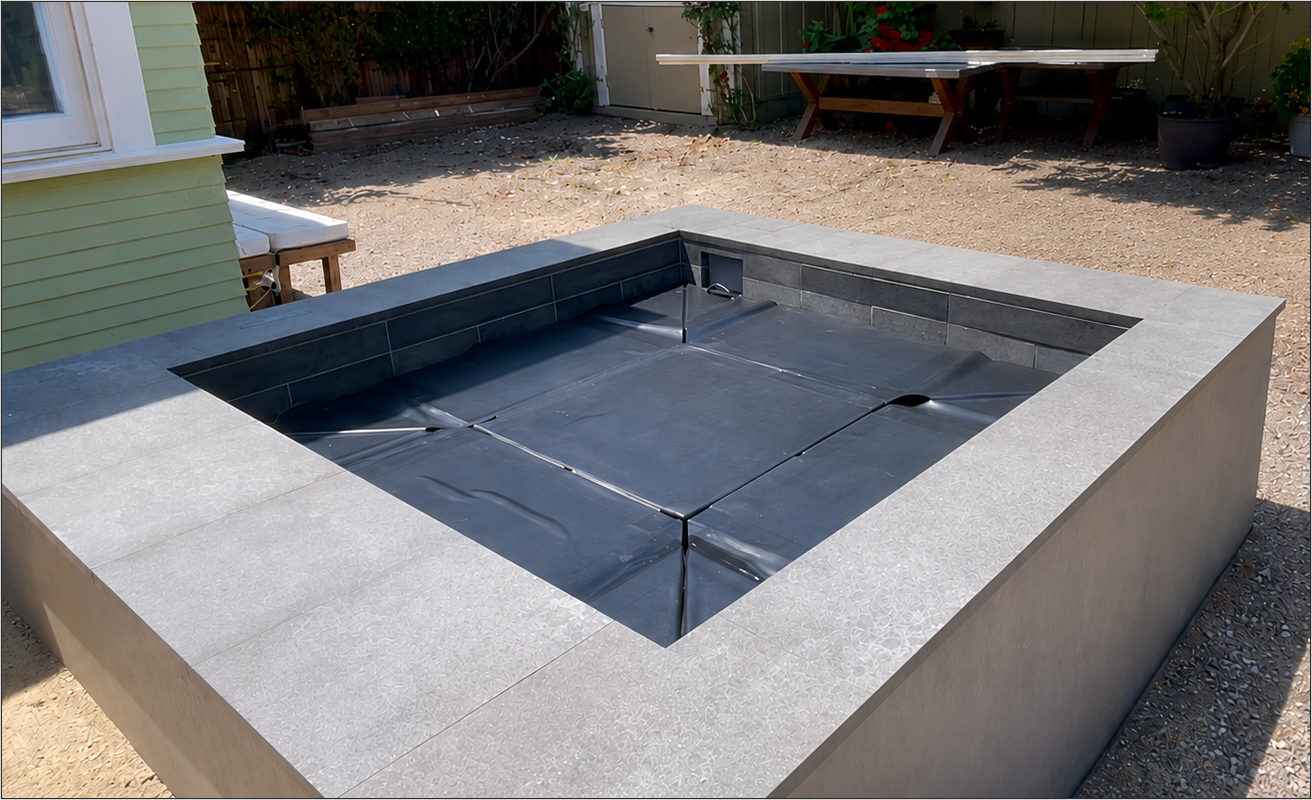
\includegraphics[
        width=5.55in,
        height=2.78in,
        keepaspectratio
    ]{deployed_functional_prototype}
};

\draw[DeepGreen,line width=0.8pt,rounded corners=7pt]
    ($(current page.north west)+(5.16in,-1.61in)$)
    rectangle
    ($(current page.north east)+(-0.42in,-4.47in)$);

\node[
    anchor=north west,
    text=Muted,
    font=\sffamily\fontsize{6.2}{6.9}\selectfont
]
at ($(current page.north west)+(5.18in,-4.54in)$)
{Functional foam model deployed over the sponsor's in-ground spa.};

% Image-strip title
\node[
    anchor=north west,
    text=DeepGreen,
    font=\sffamily\bfseries\fontsize{8.1}{8.8}\selectfont
]
at ($(current page.north west)+(0.43in,-4.78in)$)
{PRODUCT DEVELOPMENT AND FINAL ARCHITECTURE};

% Five-image development strip — CAD-first sequence
% Image 1: topside CAD
\node[anchor=center,inner sep=0pt]
at ($(current page.north west)+(1.47in,-5.73in)$)
{
    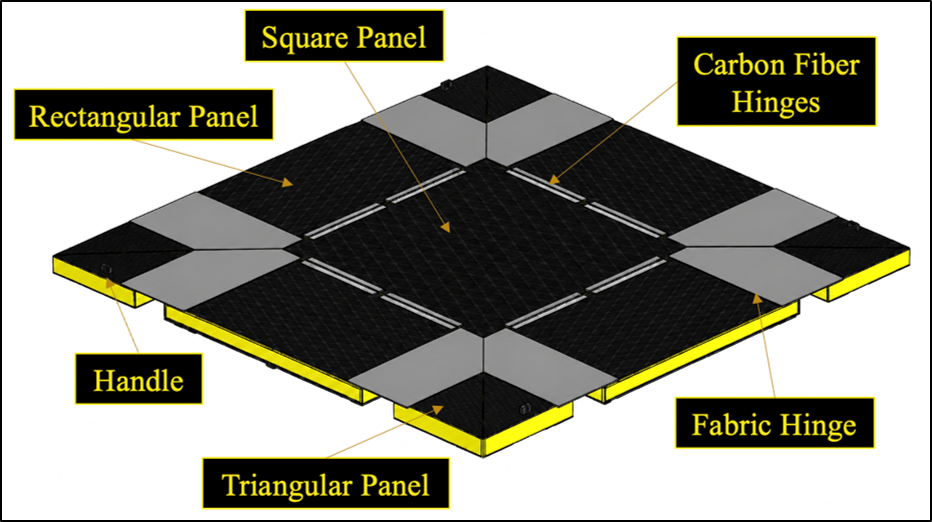
\includegraphics[
        width=1.92in,
        height=1.30in,
        keepaspectratio
    ]{Toro_Cover_topside_Cad}
};
\draw[RuleGray,line width=0.55pt,rounded corners=4pt]
    ($(current page.north west)+(0.43in,-5.04in)$)
    rectangle
    ($(current page.north west)+(2.51in,-6.43in)$);

% Image 2: underside CAD
\node[anchor=center,inner sep=0pt]
at ($(current page.north west)+(3.66in,-5.73in)$)
{
    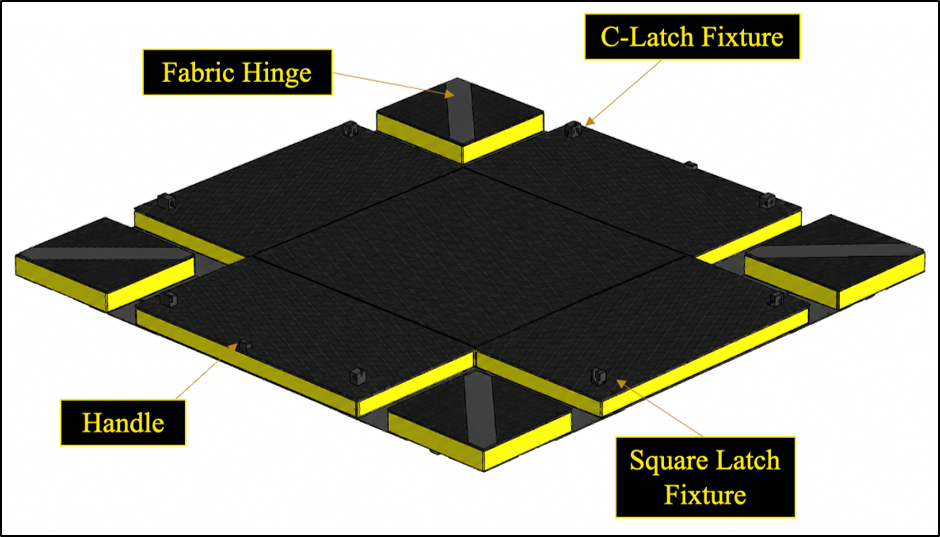
\includegraphics[
        width=1.92in,
        height=1.30in,
        keepaspectratio
    ]{toro_cover_underside_cad}
};
\draw[RuleGray,line width=0.55pt,rounded corners=4pt]
    ($(current page.north west)+(2.62in,-5.04in)$)
    rectangle
    ($(current page.north west)+(4.70in,-6.43in)$);

% Image 3: folded CAD
\node[anchor=center,inner sep=0pt]
at ($(current page.north west)+(5.85in,-5.73in)$)
{
    \includegraphics[
        width=1.92in,
        height=1.30in,
        keepaspectratio
    ]{\detokenize{Toro_Cover_folded Configuration}}
};
\draw[RuleGray,line width=0.55pt,rounded corners=4pt]
    ($(current page.north west)+(4.81in,-5.04in)$)
    rectangle
    ($(current page.north west)+(6.89in,-6.43in)$);

% Image 4: dual-use product concept
\node[anchor=center,inner sep=0pt]
at ($(current page.north west)+(8.04in,-5.73in)$)
{
    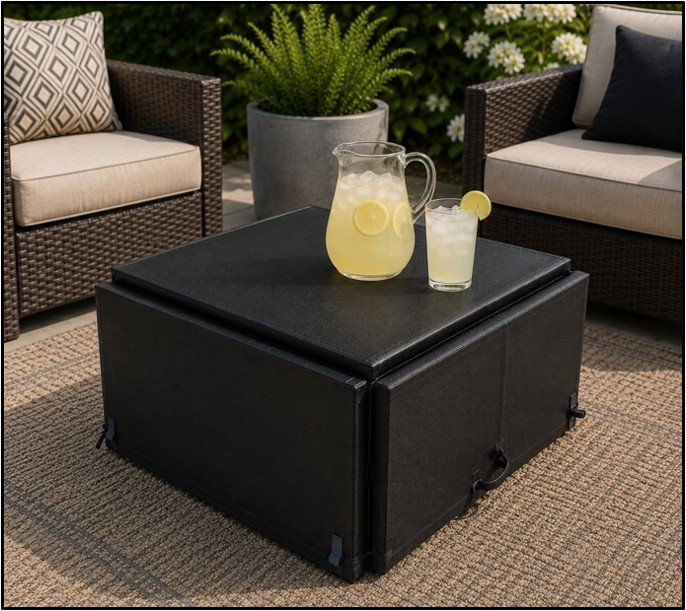
\includegraphics[
        width=1.92in,
        height=1.30in,
        keepaspectratio
    ]{generative_AI_concept_toro_cover_art}
};
\draw[RuleGray,line width=0.55pt,rounded corners=4pt]
    ($(current page.north west)+(7.00in,-5.04in)$)
    rectangle
    ($(current page.north west)+(9.08in,-6.43in)$);

% Image 5: folded foam functional prototype
% The portrait photograph is deliberately clipped to the landscape frame
% so the ottoman fills the card without extending beyond its border.
\begin{scope}
\clip[rounded corners=4pt]
    ($(current page.north west)+(9.19in,-5.04in)$)
    rectangle
    ($(current page.north east)+(-0.43in,-6.43in)$);

% Keep the original image proportions and center it within the existing card.
\node[anchor=center,inner sep=0pt]
at ($(current page.north west)+(9.88in,-5.735in)$)
{
    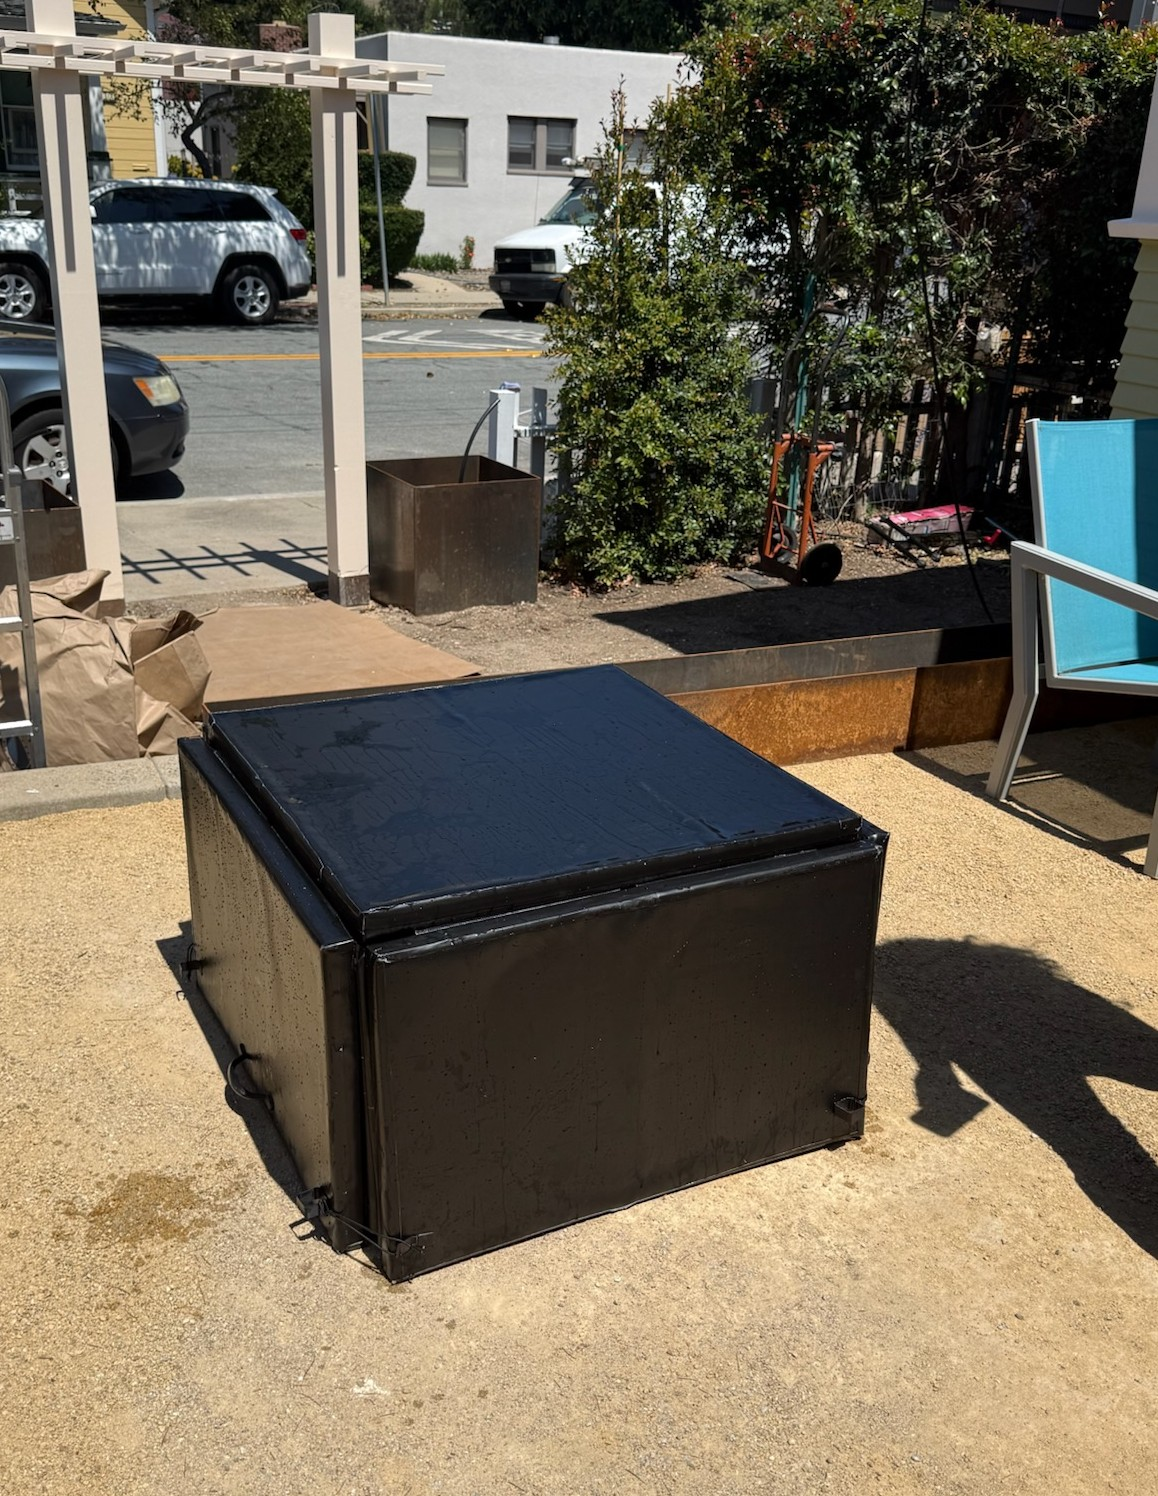
\includegraphics[
        width=1.58in,
        height=1.28in,
        keepaspectratio
    ]{foam_model_folded_backyard_image}
};
\end{scope}

\draw[RuleGray,line width=0.55pt,rounded corners=4pt]
    ($(current page.north west)+(9.19in,-5.04in)$)
    rectangle
    ($(current page.north east)+(-0.43in,-6.43in)$);

% Larger captions
\node[anchor=north,align=center,text width=1.95in,text=Muted,
      font=\sffamily\fontsize{6.8}{7.4}\selectfont]
at ($(current page.north west)+(1.47in,-6.49in)$)
{Topside panel architecture};

\node[anchor=north,align=center,text width=1.95in,text=Muted,
      font=\sffamily\fontsize{6.8}{7.4}\selectfont]
at ($(current page.north west)+(3.66in,-6.49in)$)
{Underside hinge architecture};

\node[anchor=north,align=center,text width=1.95in,text=Muted,
      font=\sffamily\fontsize{6.8}{7.4}\selectfont]
at ($(current page.north west)+(5.85in,-6.49in)$)
{Folded CAD configuration};

\node[anchor=north,align=center,text width=1.95in,text=Muted,
      font=\sffamily\fontsize{6.8}{7.4}\selectfont]
at ($(current page.north west)+(8.04in,-6.49in)$)
{Dual-use product vision};

\node[anchor=north,align=center,text width=1.95in,text=Muted,
      font=\sffamily\fontsize{6.8}{7.4}\selectfont]
at ($(current page.north west)+(9.88in,-6.49in)$)
{Folded foam prototype};

% Page 1 resource bar — centered and non-repeated resources
\fill[Panel,rounded corners=4pt]
    ($(current page.north west)+(0.43in,-7.05in)$)
    rectangle
    ($(current page.north east)+(-0.43in,-7.64in)$);
\draw[RuleGray,line width=0.5pt,rounded corners=4pt]
    ($(current page.north west)+(0.43in,-7.05in)$)
    rectangle
    ($(current page.north east)+(-0.43in,-7.64in)$);

\node[
    anchor=center,
    align=center,
    text=DeepGreen,
    font=\sffamily\bfseries\fontsize{6.9}{7.5}\selectfont
]
at ($(current page.north)+(0,-7.345in)$)
{\href{\ToroDrawingLink}{\faDraftingCompass\ DRAWING PACKAGE}
\hspace{24pt}
\href{\ToroDimensionsLink}{\faImage\ DIMENSION STUDY}
\hspace{24pt}
\href{\ToroProblemLink}{\faFileImage\ PROBLEM STATEMENT}};

% Footer
\node[
    anchor=south west,
    text=white,
    font=\sffamily\bfseries\fontsize{7.1}{7.7}\selectfont
]
at ($(current page.south west)+(0.42in,0.17in)$)
{\hyperlink{composites}{\faArrowLeft\ COMPOSITES}};

\node[
    anchor=south,
    text=white,
    font=\sffamily\fontsize{7.0}{7.6}\selectfont
]
at ($(current page.south)+(0,0.17in)$)
{TORO COVER \hspace{6pt} 1 / 3};

\node[
    anchor=south east,
    text=white,
    font=\sffamily\bfseries\fontsize{7.1}{7.7}\selectfont
]
at ($(current page.south east)+(-0.42in,0.17in)$)
{MANUFACTURING-DRIVEN DESIGN \faArrowRight};

\end{tikzpicture}


% ============================================================
% PAGE 2 — MANUFACTURING-DRIVEN DESIGN
% ============================================================

\clearpage
\thispagestyle{empty}
\hypertarget{toro-manufacturing}{}
\null

\begin{tikzpicture}[remember picture,overlay]

% Background and bars
\fill[white]
    (current page.south west)
    rectangle
    (current page.north east);

\fill[DeepGreen]
    (current page.north west)
    rectangle
    ($(current page.north east)+(0,-0.095in)$);

\fill[PolyGold]
    ($(current page.north west)+(0,-0.095in)$)
    rectangle
    ($(current page.north east)+(0,-0.14in)$);

\fill[DeepGreen]
    (current page.south west)
    rectangle
    ($(current page.south east)+(0,0.36in)$);

\fill[PolyGold]
    ($(current page.south west)+(0,0.36in)$)
    rectangle
    ($(current page.south east)+(0,0.405in)$);

% Header
\node[
    anchor=north west,
    text=PolyGold,
    font=\sffamily\bfseries\fontsize{8.1}{8.7}\selectfont
]
at ($(current page.north west)+(0.42in,-0.39in)$)
{TORO COVER \hspace{5pt}/\hspace{5pt} DESIGN FOR MANUFACTURABILITY};

\node[
    anchor=north west,
    text=DeepGreen,
    font=\bfseries\fontsize{23}{24}\selectfont
]
at ($(current page.north west)+(0.40in,-0.67in)$)
{THE ENVELOPE METHOD};

\node[
    anchor=north west,
    text=Muted,
    font=\sffamily\fontsize{8.7}{9.6}\selectfont
]
at ($(current page.north west)+(0.42in,-1.12in)$)
{A one-layup process developed for unusually thick insulated composite sandwich panels};

\fill[PolyGold]
    ($(current page.north west)+(0.42in,-1.36in)$)
    rectangle
    ($(current page.north west)+(5.30in,-1.315in)$);

% Process explanation
\fill[SoftGold,rounded corners=5pt]
    ($(current page.north west)+(0.42in,-1.61in)$)
    rectangle
    ($(current page.north east)+(-0.42in,-2.90in)$);

\fill[PolyGold]
    ($(current page.north west)+(0.42in,-1.61in)$)
    rectangle
    ($(current page.north west)+(0.52in,-2.90in)$);

\node[
    anchor=north west,
    text=DeepGreen,
    font=\sffamily\bfseries\fontsize{7.9}{8.6}\selectfont
]
at ($(current page.north west)+(0.67in,-1.76in)$)
{PROCESS INNOVATION};

\node[
    anchor=north west,
    align=left,
    text width=9.55in,
    text=Ink,
    font=\fontsize{7.35}{8.75}\selectfont
]
at ($(current page.north west)+(0.67in,-2.02in)$)
{
Weight reduction and insulation were both essential, leading to the selection of an
XPS foam core. Because XPS could not tolerate composite heat-cure temperatures, prepreg
processing was not practical and the panels had to be manufactured by wet layup with a
room-temperature cure. To simplify this process, I waterjet-cut XPS perimeter strips from
excess foam and placed them around each core inside the vacuum enclosure. Under vacuum,
the top and bottom carbon skins met along the panel sides and compressed against this
border, eliminating a separate edge-banding layup and reducing corner pleating.
};

% Workflow title
\node[
    anchor=north west,
    text=DeepGreen,
    font=\sffamily\bfseries\fontsize{8.0}{8.7}\selectfont
]
at ($(current page.north west)+(0.43in,-3.06in)$)
{MANUFACTURING WORKFLOW};

% Row 1 image 1
\node[anchor=center,inner sep=0pt]
at ($(current page.north west)+(2.07in,-4.105in)$)
{
    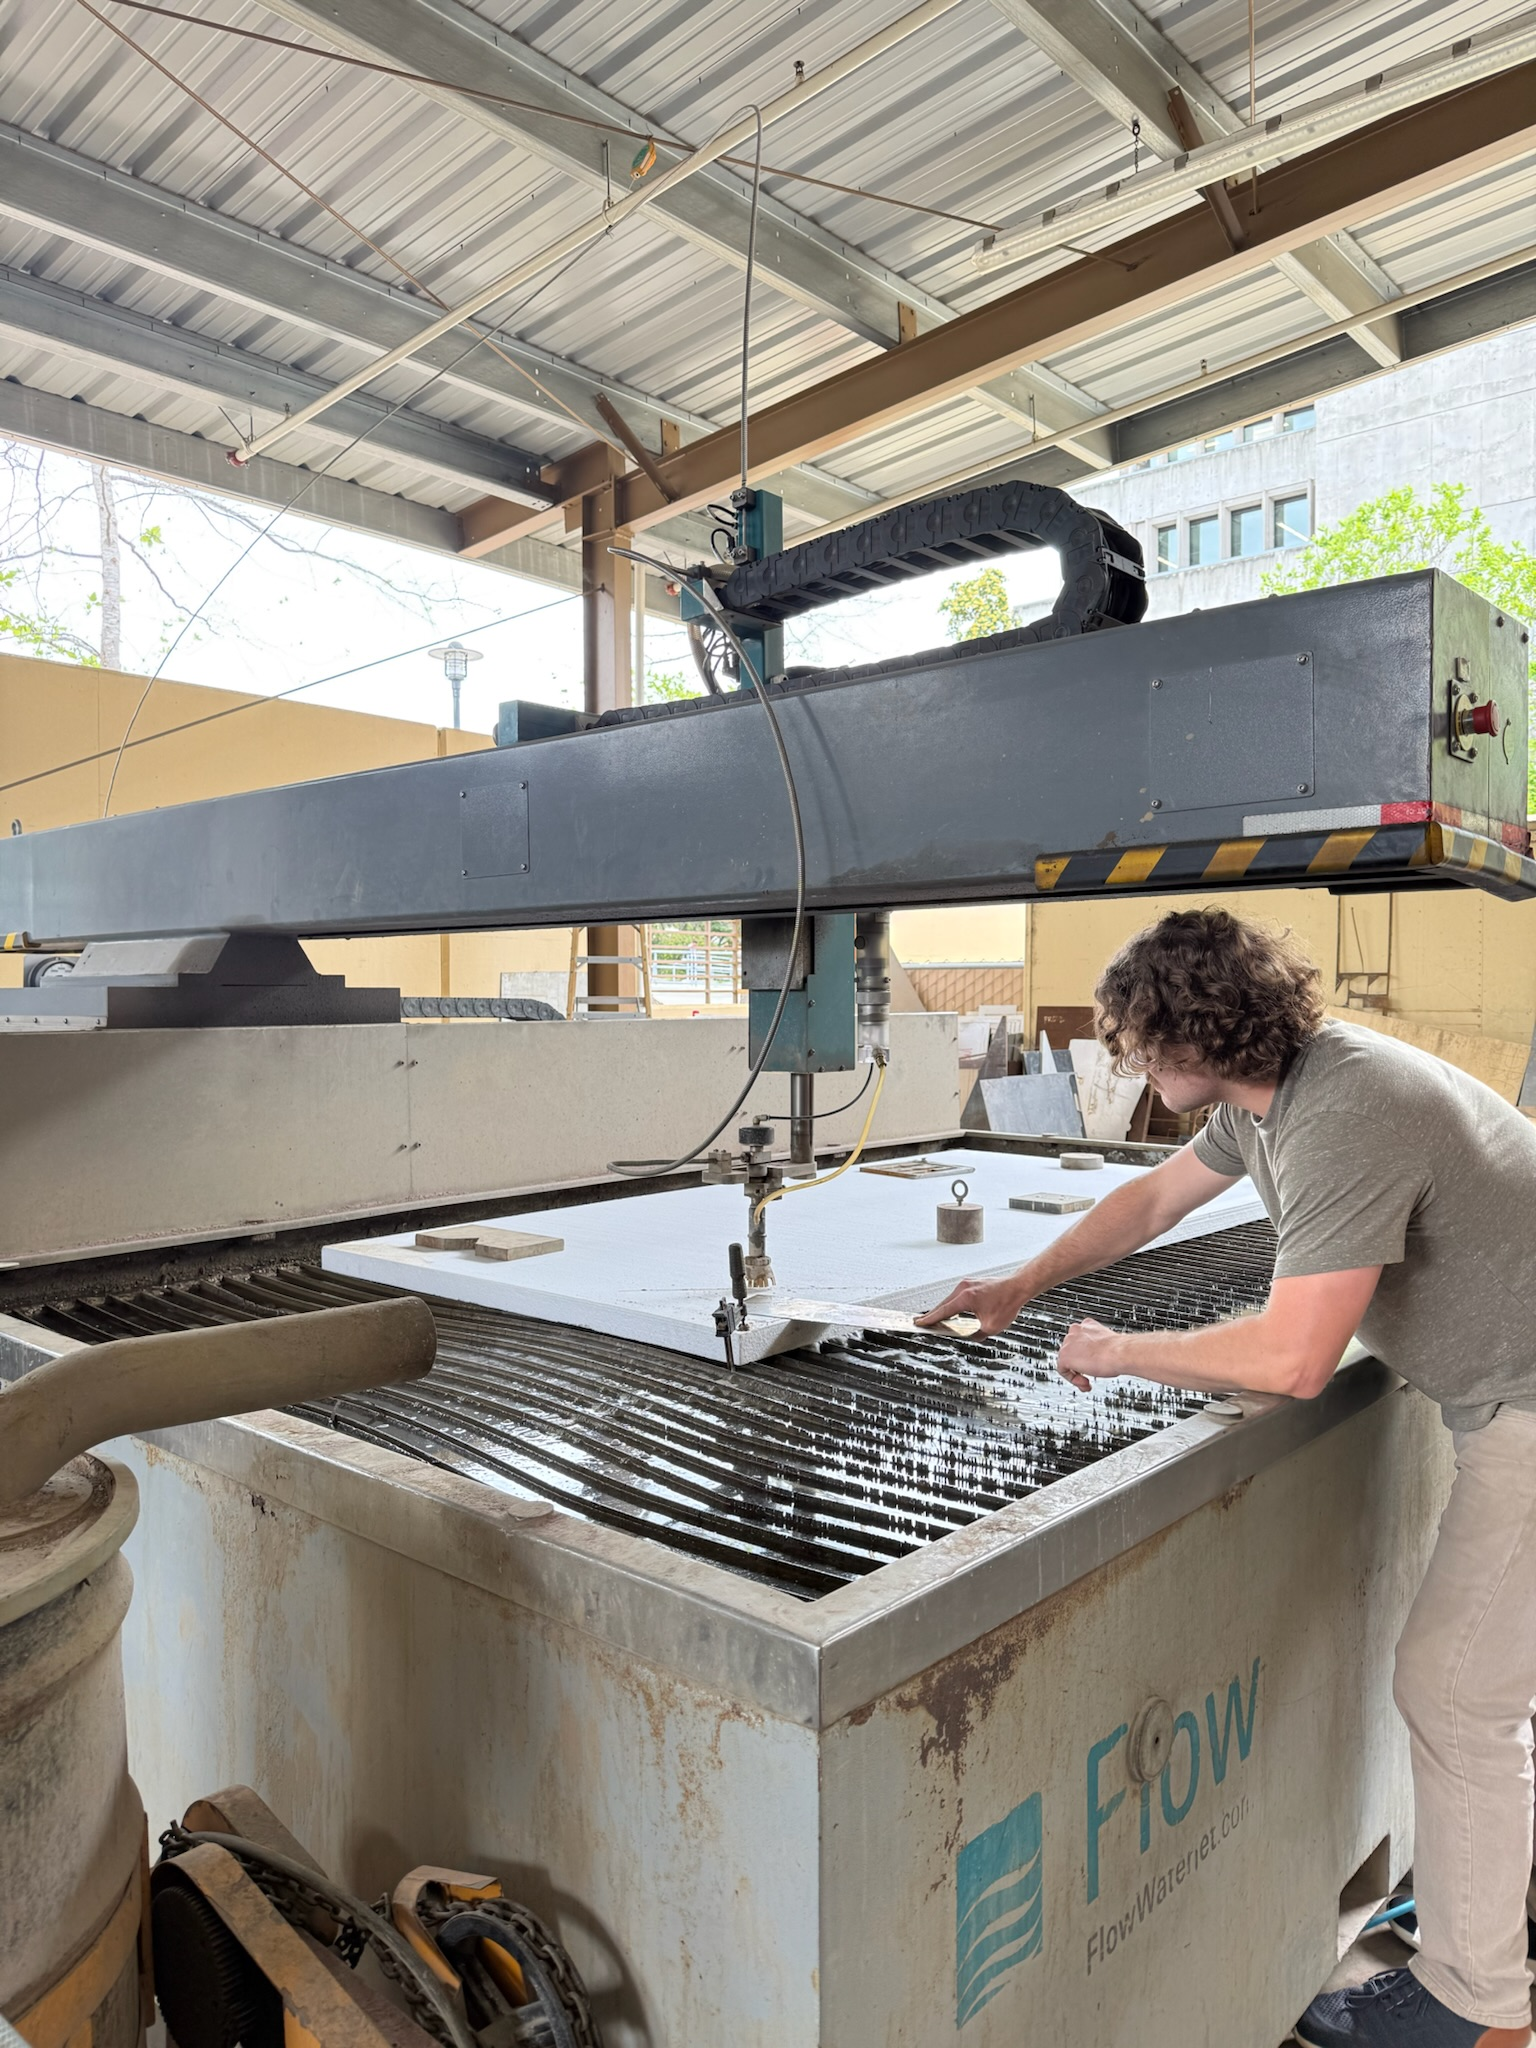
\includegraphics[
        width=3.10in,
        height=1.40in,
        keepaspectratio
    ]{waterjet_foam}
};
\draw[RuleGray,line width=0.55pt,rounded corners=4pt]
    ($(current page.north west)+(0.43in,-3.36in)$)
    rectangle
    ($(current page.north west)+(3.71in,-4.85in)$);

% Row 1 image 2
\node[anchor=center,inner sep=0pt]
at ($(current page.north west)+(5.50in,-4.105in)$)
{
    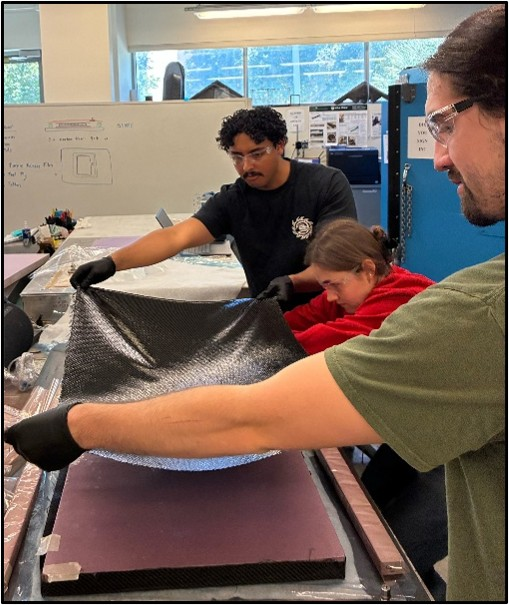
\includegraphics[
        width=3.10in,
        height=1.40in,
        keepaspectratio
    ]{group_layup}
};
\draw[RuleGray,line width=0.55pt,rounded corners=4pt]
    ($(current page.north west)+(3.86in,-3.36in)$)
    rectangle
    ($(current page.north west)+(7.14in,-4.85in)$);

% Row 1 image 3
\node[anchor=center,inner sep=0pt]
at ($(current page.north west)+(8.935in,-4.105in)$)
{
    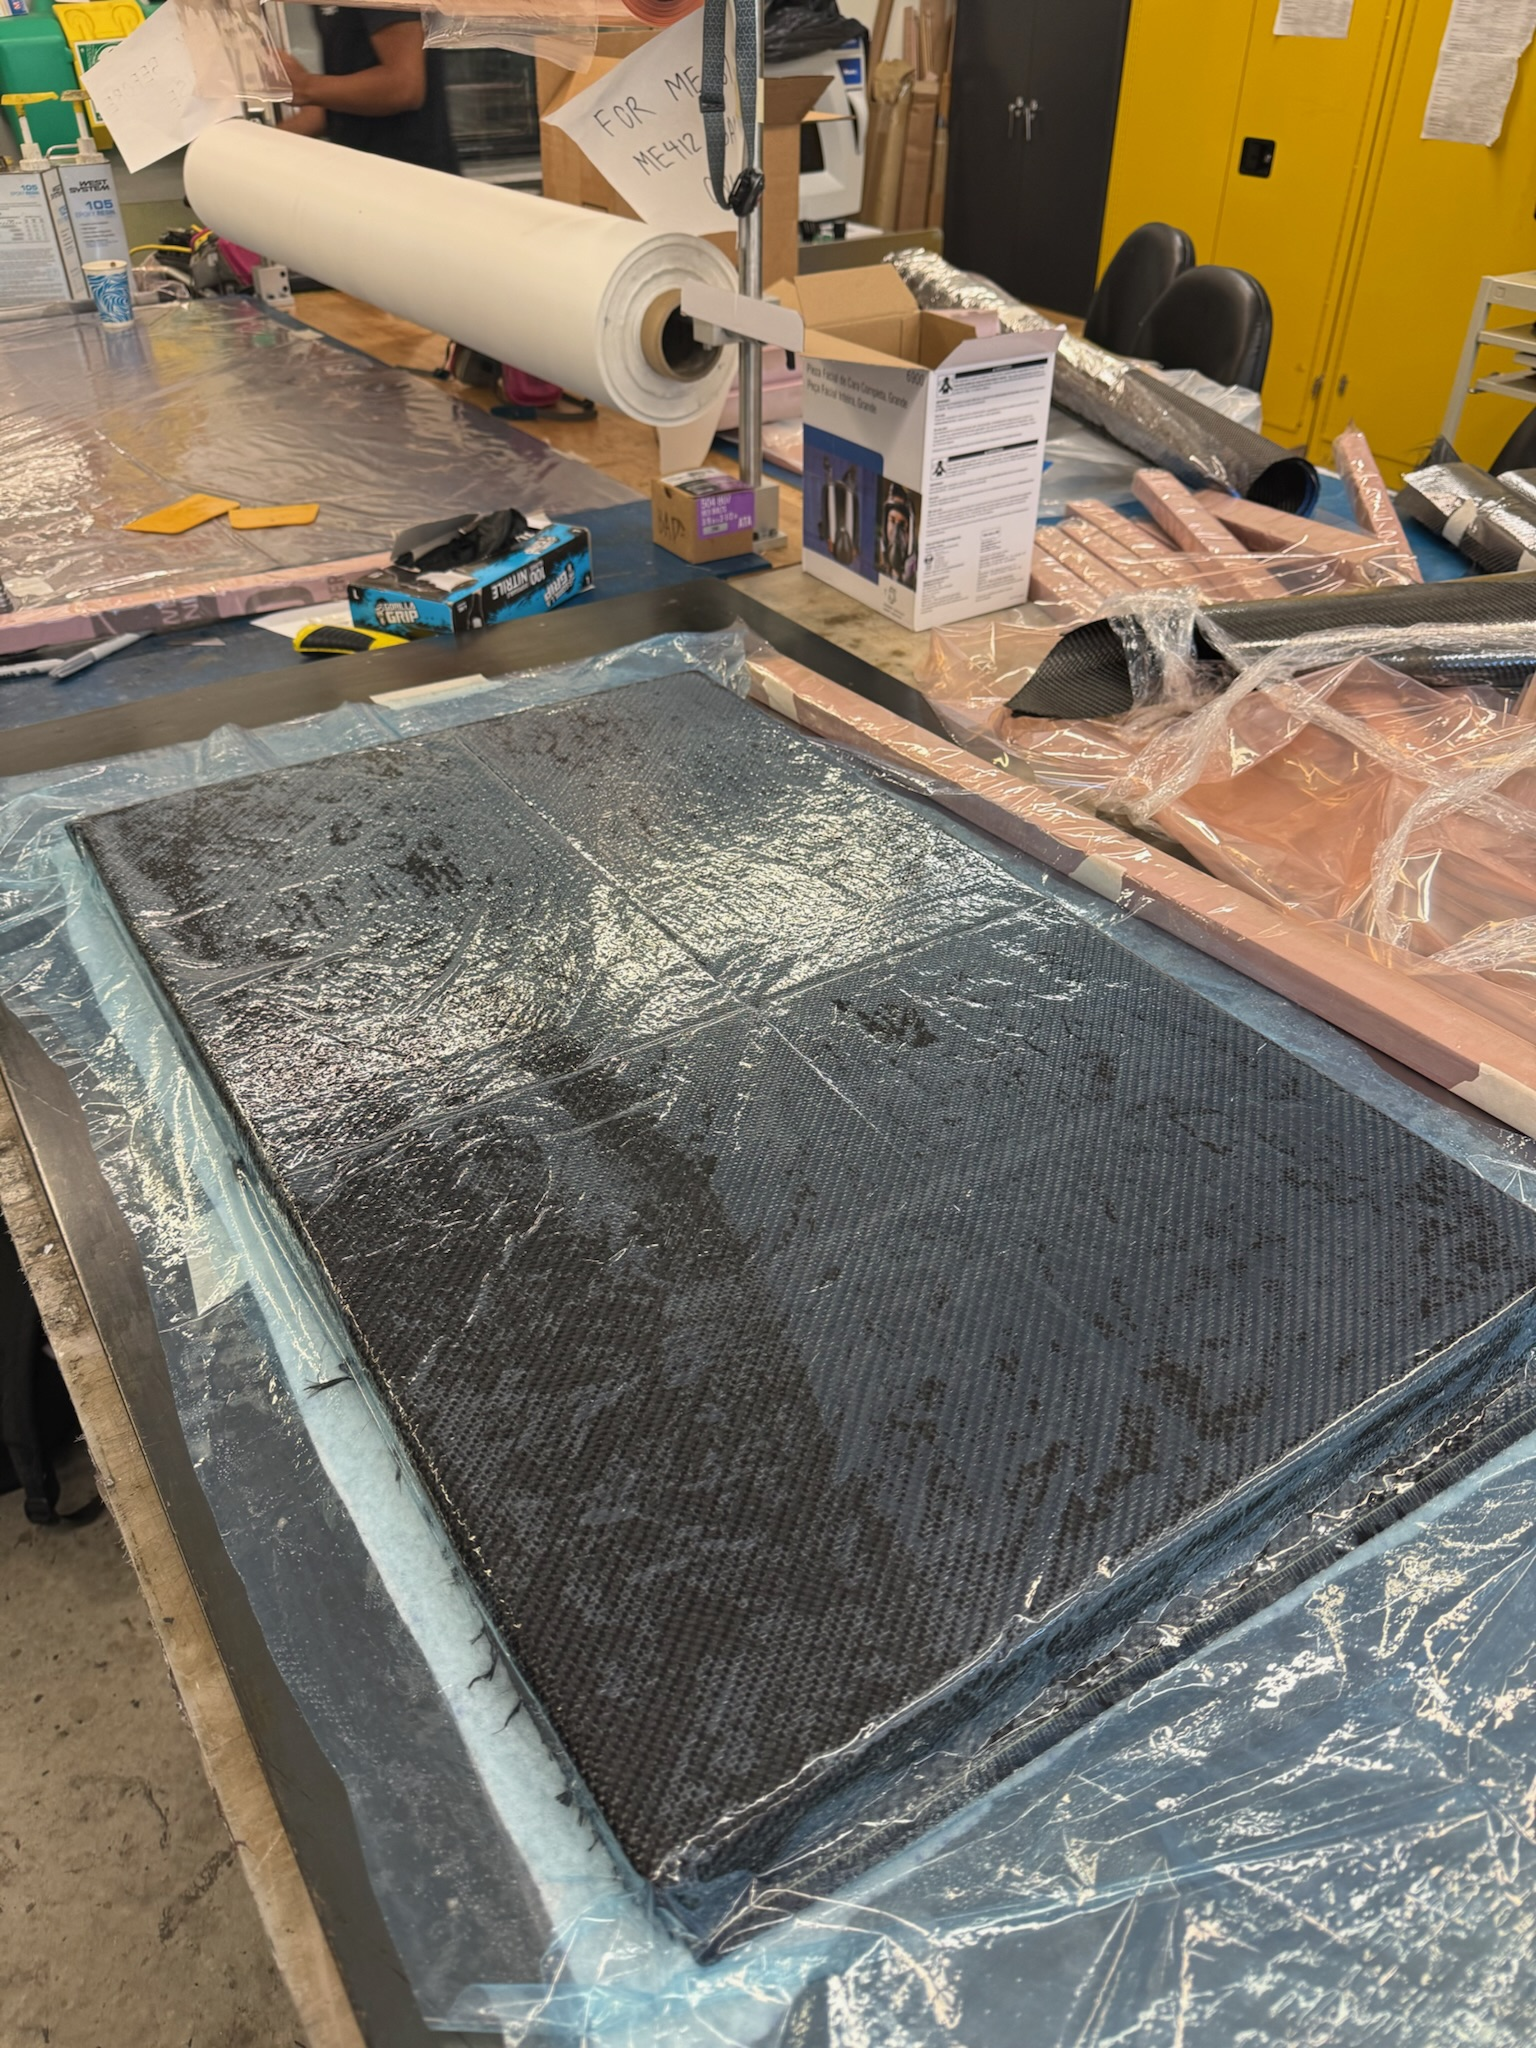
\includegraphics[
        width=3.10in,
        height=1.40in,
        keepaspectratio
    ]{blue_perforrated_film_layup}
};
\draw[RuleGray,line width=0.55pt,rounded corners=4pt]
    ($(current page.north west)+(7.29in,-3.36in)$)
    rectangle
    ($(current page.north east)+(-0.42in,-4.85in)$);

% Row 1 captions
\node[anchor=north,text=Muted,font=\sffamily\fontsize{6.7}{7.3}\selectfont]
at ($(current page.north west)+(2.07in,-4.90in)$)
{1. Waterjet-cut core and perimeter geometry};

\node[anchor=north,text=Muted,font=\sffamily\fontsize{6.7}{7.3}\selectfont]
at ($(current page.north west)+(5.50in,-4.90in)$)
{2. Team wet layup under my process guidance};

\node[anchor=north,text=Muted,font=\sffamily\fontsize{6.7}{7.3}\selectfont]
at ($(current page.north west)+(8.935in,-4.90in)$)
{3. Perforated film, breather, and vacuum enclosure};

% Row 2 image 1
\node[anchor=center,inner sep=0pt]
at ($(current page.north west)+(2.07in,-5.875in)$)
{
    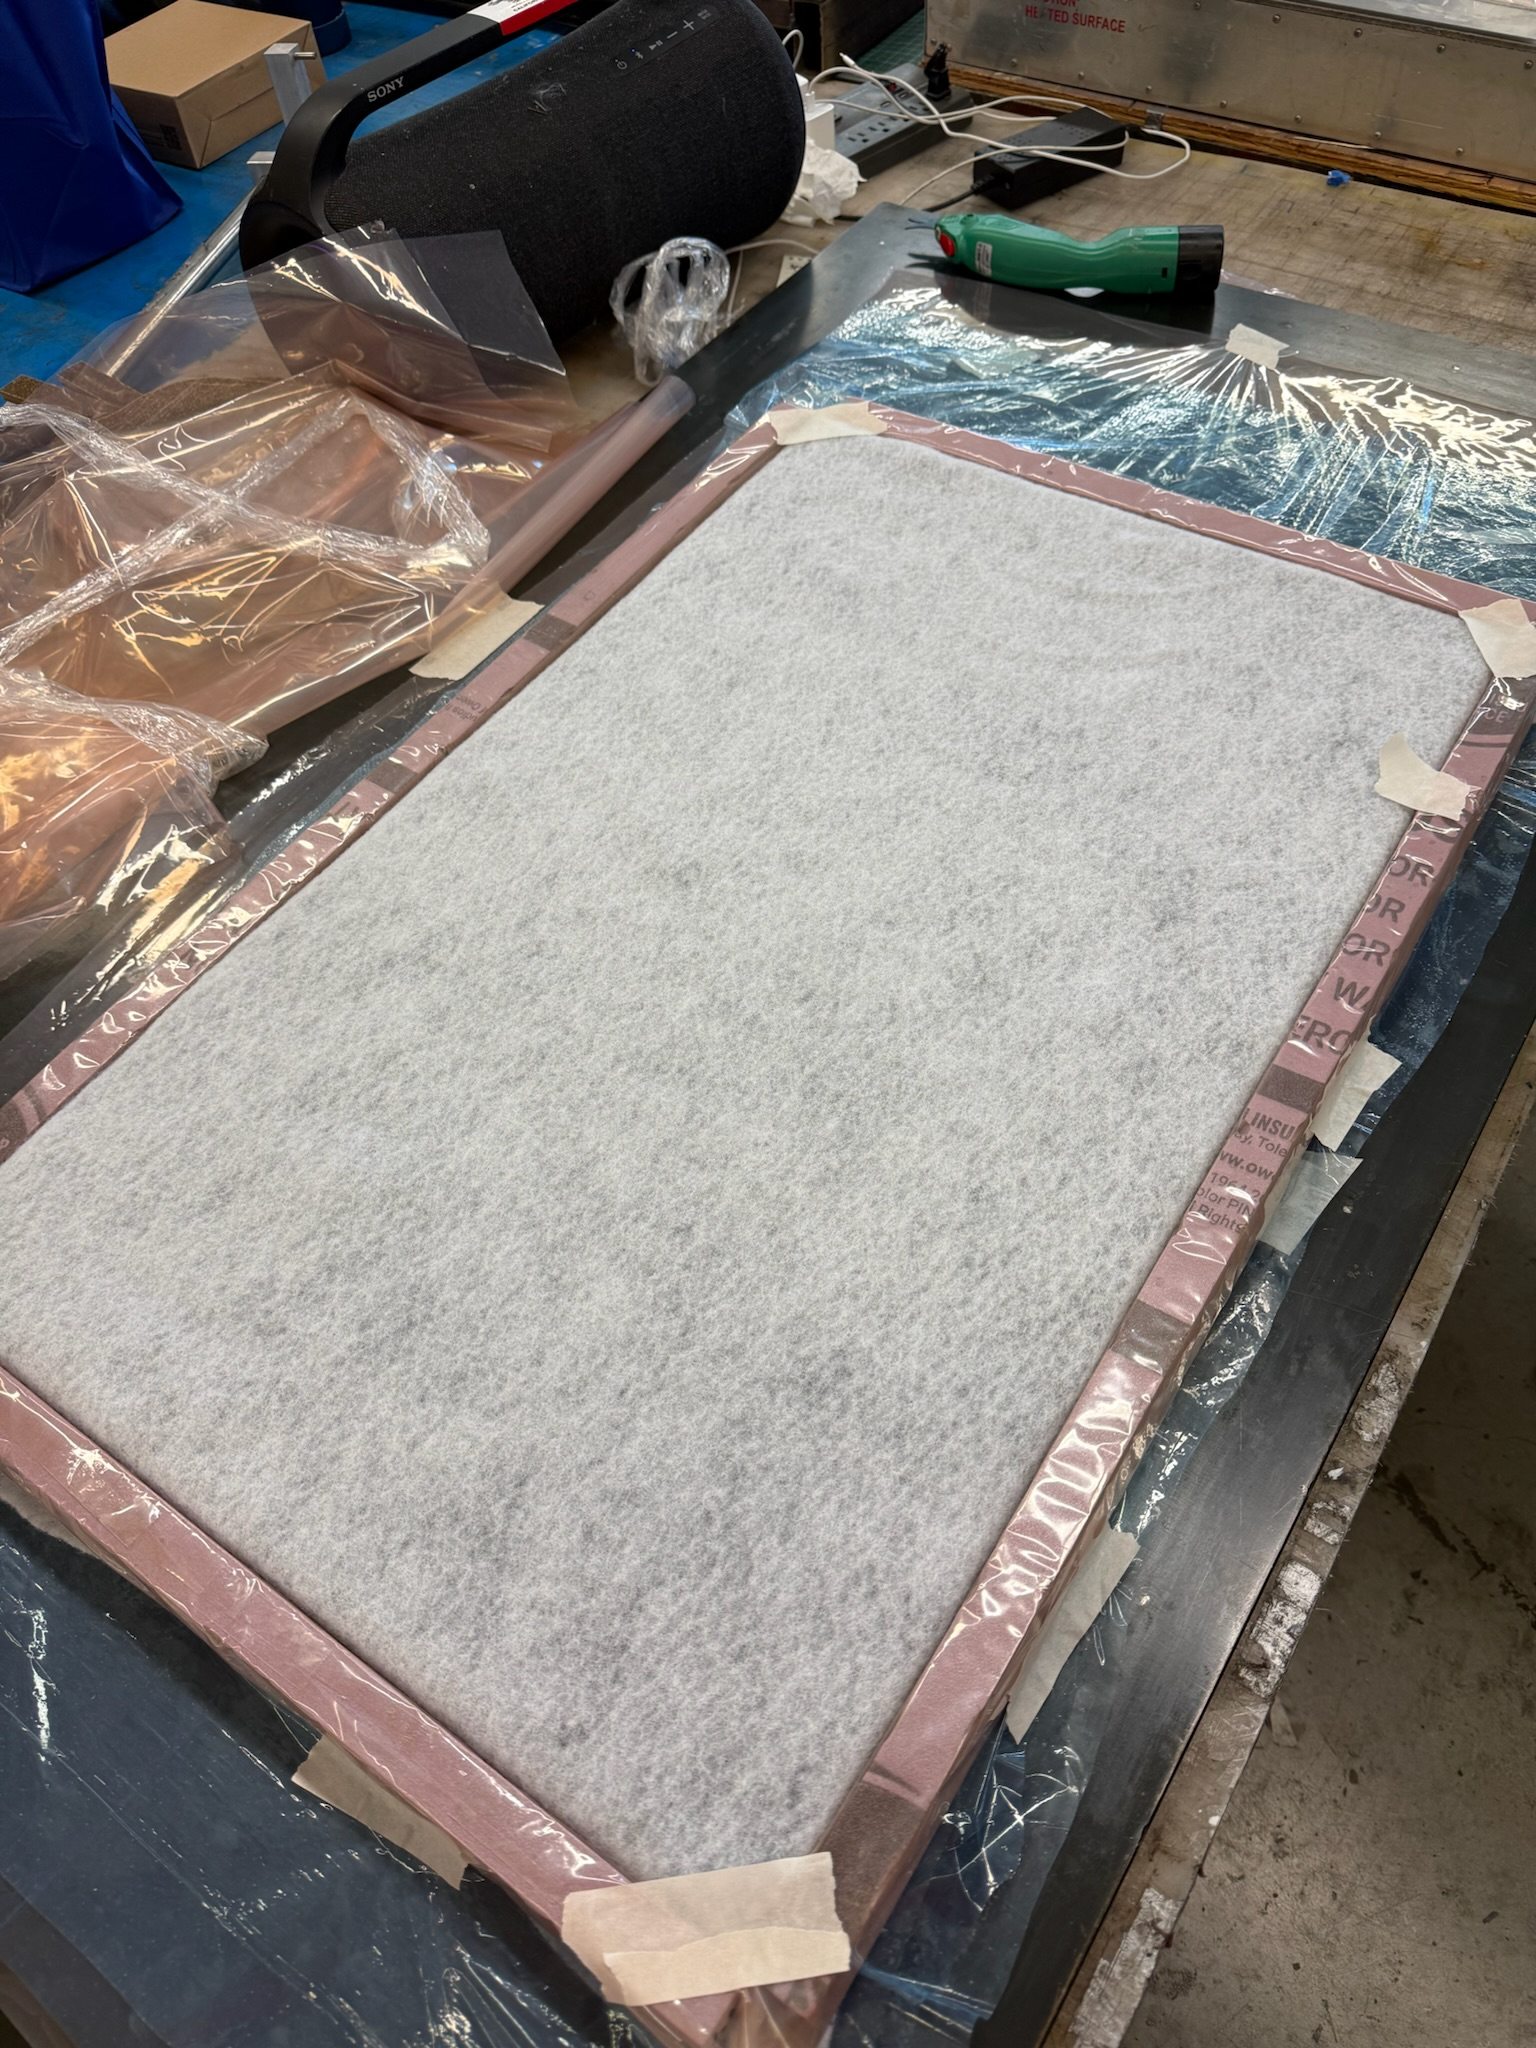
\includegraphics[
        width=3.10in,
        height=1.40in,
        keepaspectratio
    ]{completed_layup}
};
\draw[RuleGray,line width=0.55pt,rounded corners=4pt]
    ($(current page.north west)+(0.43in,-5.13in)$)
    rectangle
    ($(current page.north west)+(3.71in,-6.62in)$);

% Row 2 image 2 — oven chamber used only as a reliable vacuum enclosure; no heat applied
\node[anchor=center,inner sep=0pt]
at ($(current page.north west)+(5.50in,-5.875in)$)
{
    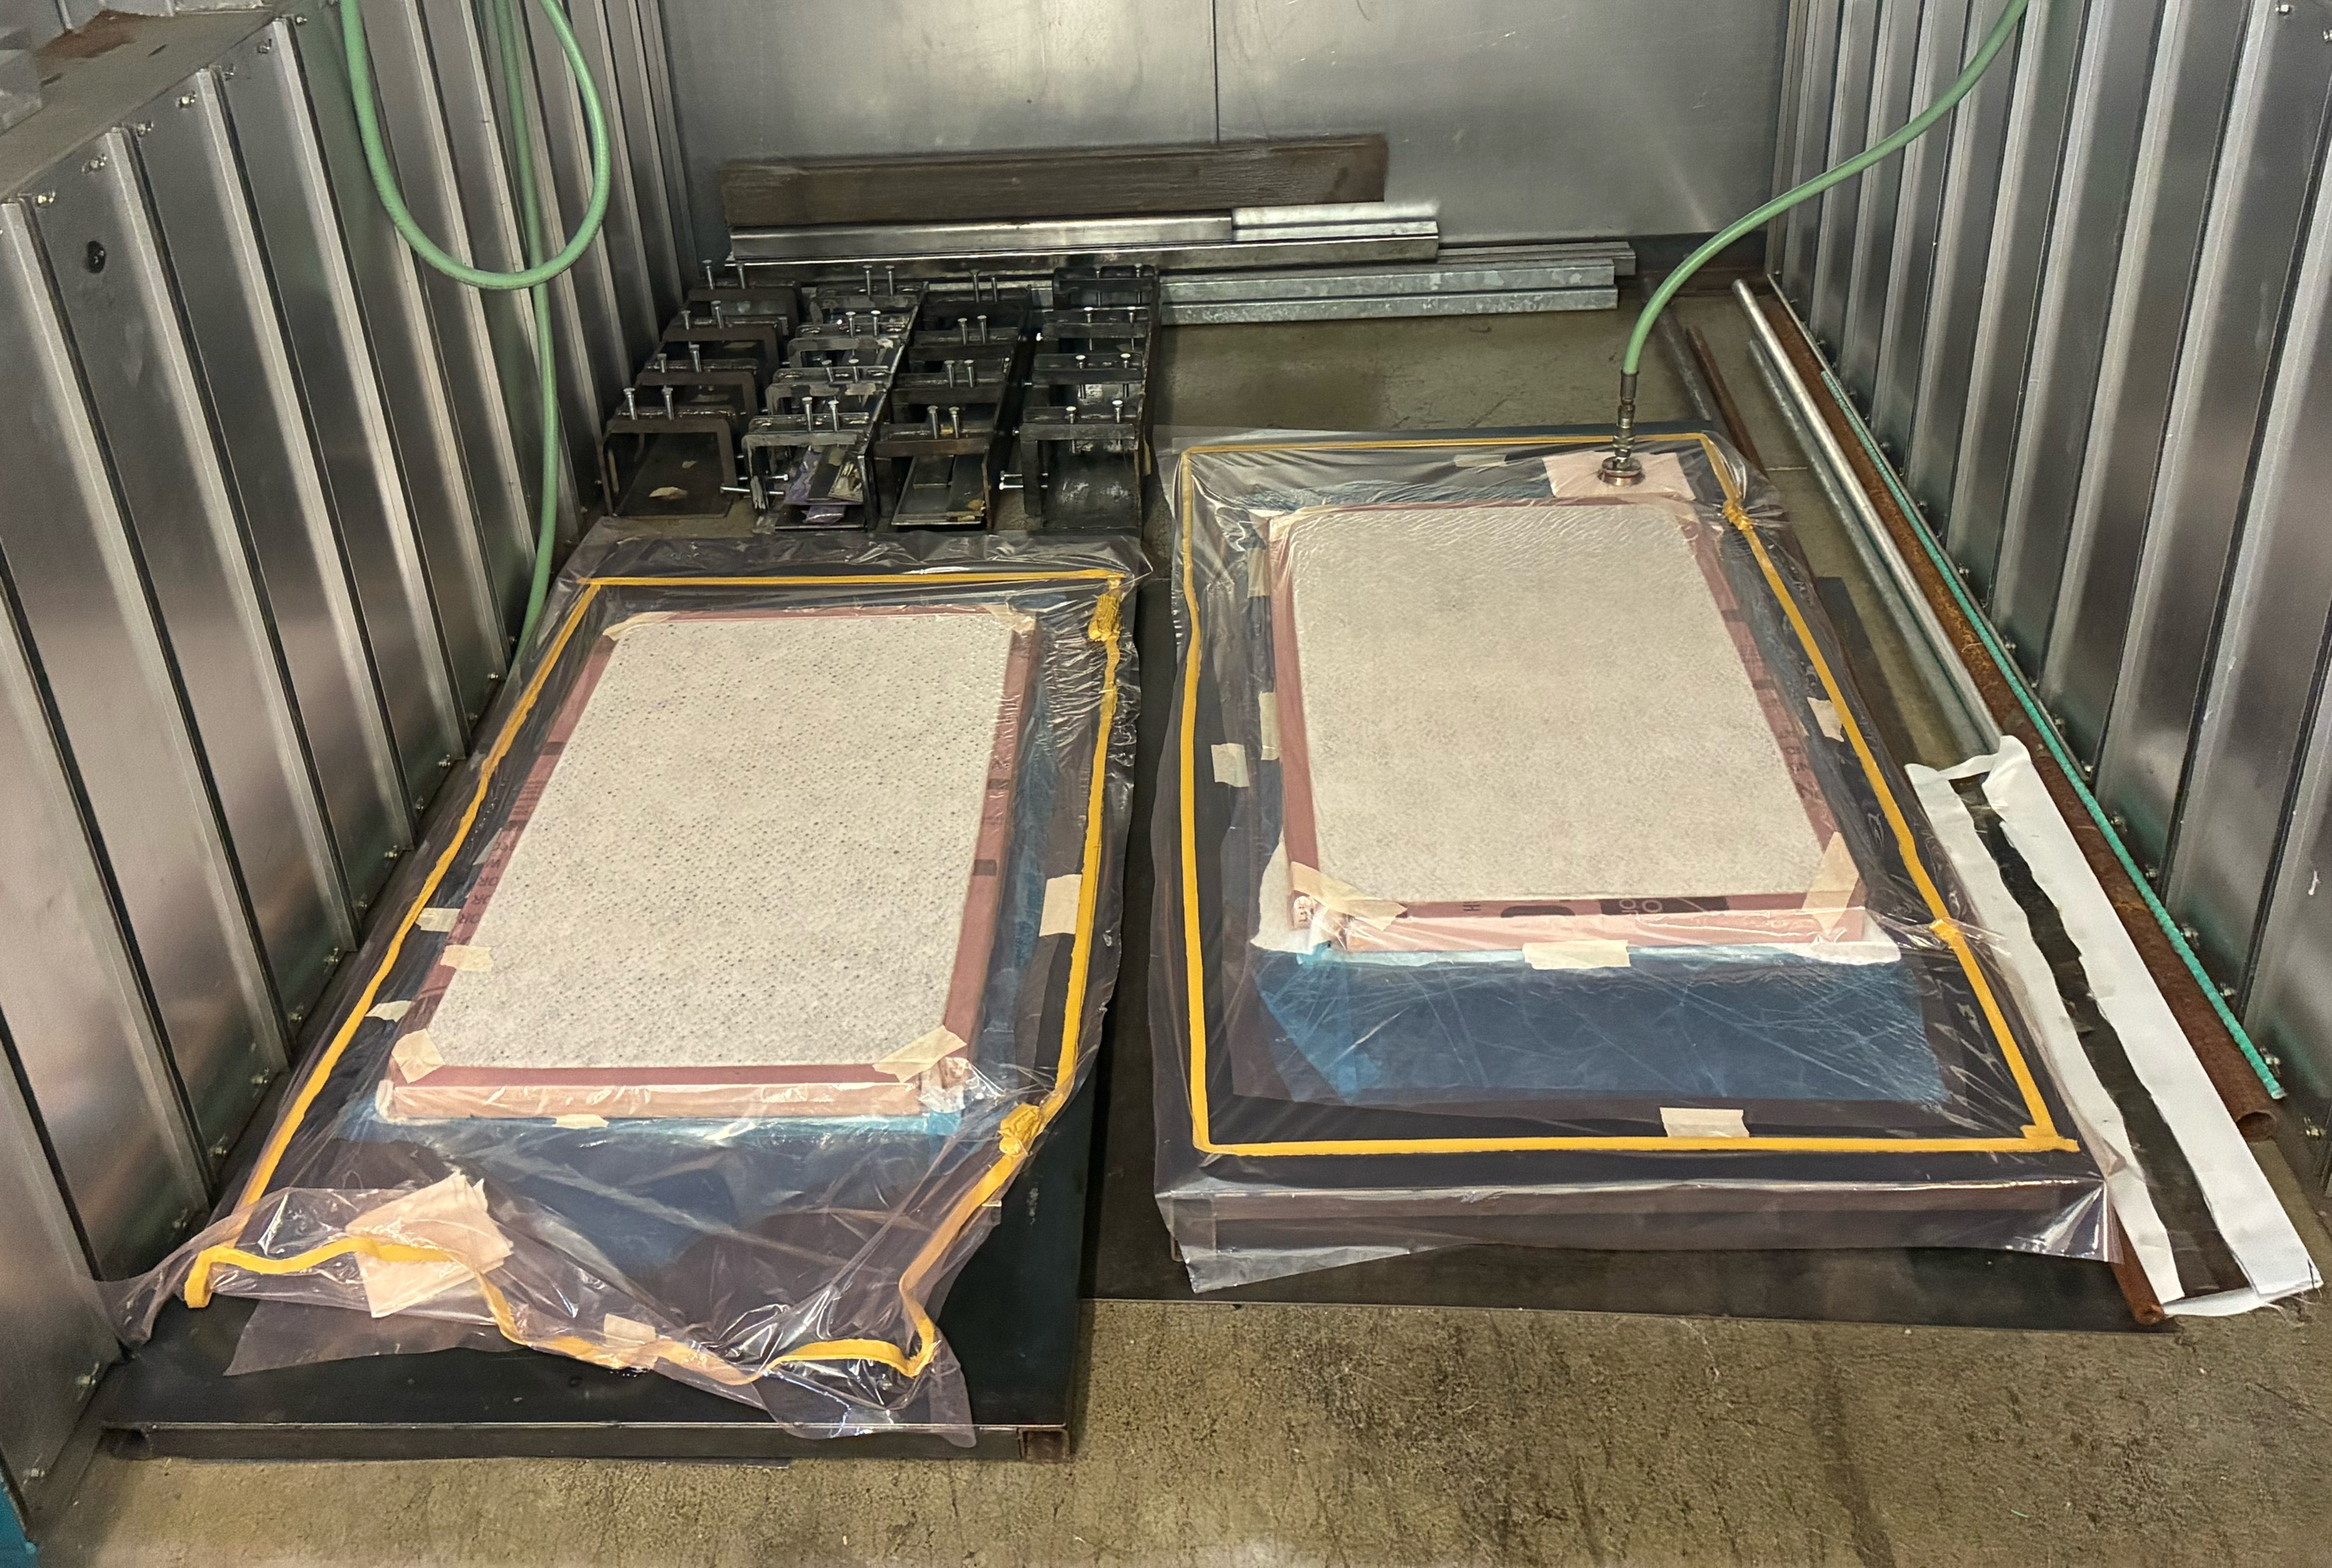
\includegraphics[
        width=3.10in,
        height=1.40in,
        keepaspectratio
    ]{layups_in_composite_oven_under_vacuumPressure}
};
\draw[RuleGray,line width=0.55pt,rounded corners=4pt]
    ($(current page.north west)+(3.86in,-5.13in)$)
    rectangle
    ($(current page.north west)+(7.14in,-6.62in)$);

% Row 2 image 3
\node[anchor=center,inner sep=0pt]
at ($(current page.north west)+(8.935in,-5.875in)$)
{
    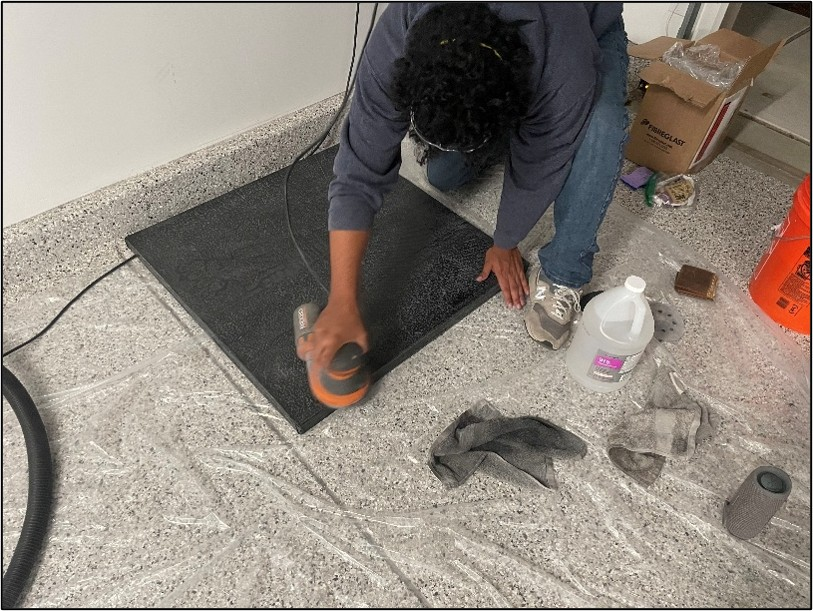
\includegraphics[
        width=3.10in,
        height=1.40in,
        keepaspectratio
    ]{garage_sanding}
};
\draw[RuleGray,line width=0.55pt,rounded corners=4pt]
    ($(current page.north west)+(7.29in,-5.13in)$)
    rectangle
    ($(current page.north east)+(-0.42in,-6.62in)$);

% Row 2 captions
\node[anchor=north,text=Muted,font=\sffamily\fontsize{6.7}{7.3}\selectfont]
at ($(current page.north west)+(2.07in,-6.67in)$)
{4. Fully saturated carbon skin and foam sandwich};

\node[anchor=north,text=Muted,font=\sffamily\fontsize{6.7}{7.3}\selectfont]
at ($(current page.north west)+(5.50in,-6.67in)$)
{5. Room-temperature cure under continuous vacuum};

\node[anchor=north,text=Muted,font=\sffamily\fontsize{6.7}{7.3}\selectfont]
at ($(current page.north west)+(8.935in,-6.67in)$)
{6. Post-processing and surface preparation};

% Bottom callouts
\fill[Panel,rounded corners=4pt]
    ($(current page.north west)+(0.43in,-6.95in)$)
    rectangle
    ($(current page.north west)+(5.48in,-7.60in)$);

\draw[RuleGray,line width=0.55pt,rounded corners=4pt]
    ($(current page.north west)+(0.43in,-6.95in)$)
    rectangle
    ($(current page.north west)+(5.48in,-7.60in)$);

\node[
    anchor=north west,
    text=DeepGreen,
    font=\sffamily\bfseries\fontsize{7.0}{7.6}\selectfont
]
at ($(current page.north west)+(0.63in,-7.08in)$)
{FROM THREE LAYUPS TO ONE};

\node[
    anchor=north west,
    align=left,
    text width=4.56in,
    text=Ink,
    font=\fontsize{6.45}{7.45}\selectfont
]
at ($(current page.north west)+(0.63in,-7.29in)$)
{
The Envelope Method reduced labor, cure cycles, handling,
alignment risk, and time spent forming numerous vacuum-bag
pleats around the 1.5-inch-thick XPS panels.
};

\fill[Panel,rounded corners=4pt]
    ($(current page.north west)+(5.68in,-6.95in)$)
    rectangle
    ($(current page.north east)+(-0.42in,-7.60in)$);

\draw[RuleGray,line width=0.55pt,rounded corners=4pt]
    ($(current page.north west)+(5.68in,-6.95in)$)
    rectangle
    ($(current page.north east)+(-0.42in,-7.60in)$);

\node[
    anchor=north west,
    text=DeepGreen,
    font=\sffamily\bfseries\fontsize{7.0}{7.6}\selectfont
]
at ($(current page.north west)+(5.88in,-7.08in)$)
{WHY SURFACE-BONDED HARDWARE};

\node[
    anchor=north west,
    align=left,
    text width=4.55in,
    text=Ink,
    font=\fontsize{6.45}{7.45}\selectfont
]
at ($(current page.north west)+(5.88in,-7.29in)$)
{
Adhesively bonded hinges and fixtures preserved the clean
composite exterior and avoided drilled inserts, foam-core
crushing, added stress concentrations, and new leak paths.
};


% Footer
\node[
    anchor=south west,
    text=white,
    font=\sffamily\bfseries\fontsize{7.1}{7.7}\selectfont
]
at ($(current page.south west)+(0.42in,0.17in)$)
{\faArrowLeft\ PRODUCT ARCHITECTURE};

\node[
    anchor=south,
    text=white,
    font=\sffamily\fontsize{7.0}{7.6}\selectfont
]
at ($(current page.south)+(0,0.17in)$)
{TORO COVER \hspace{6pt} 2 / 3};

\node[
    anchor=south east,
    text=white,
    font=\sffamily\bfseries\fontsize{7.1}{7.7}\selectfont
]
at ($(current page.south east)+(-0.42in,0.17in)$)
{VALIDATION \& TAKEAWAYS \faArrowRight};

\end{tikzpicture}


% ============================================================
% PAGE 3 — FINISHING, VALIDATION, AND TAKEAWAYS
% ============================================================

\clearpage
\thispagestyle{empty}
\hypertarget{toro-results}{}
\null

\begin{tikzpicture}[remember picture,overlay]

% Background and bars
\fill[white]
    (current page.south west)
    rectangle
    (current page.north east);

\fill[DeepGreen]
    (current page.north west)
    rectangle
    ($(current page.north east)+(0,-0.095in)$);

\fill[PolyGold]
    ($(current page.north west)+(0,-0.095in)$)
    rectangle
    ($(current page.north east)+(0,-0.14in)$);

\fill[DeepGreen]
    (current page.south west)
    rectangle
    ($(current page.south east)+(0,0.36in)$);

\fill[PolyGold]
    ($(current page.south west)+(0,0.36in)$)
    rectangle
    ($(current page.south east)+(0,0.405in)$);

% Header
\node[
    anchor=north west,
    text=PolyGold,
    font=\sffamily\bfseries\fontsize{8.1}{8.7}\selectfont
]
at ($(current page.north west)+(0.42in,-0.39in)$)
{TORO COVER \hspace{5pt}/\hspace{5pt} VALIDATION AND ENGINEERING TAKEAWAYS};

\node[
    anchor=north west,
    text=DeepGreen,
    font=\bfseries\fontsize{22.5}{23.5}\selectfont
]
at ($(current page.north west)+(0.40in,-0.67in)$)
{FROM PROTOTYPE TO PRODUCT PATHWAY};

\node[
    anchor=north west,
    text=Muted,
    font=\sffamily\fontsize{8.7}{9.6}\selectfont
]
at ($(current page.north west)+(0.42in,-1.12in)$)
{Environmental protection, usability testing, scope decisions, and lessons from technical leadership};

\fill[PolyGold]
    ($(current page.north west)+(0.42in,-1.36in)$)
    rectangle
    ($(current page.north west)+(5.8in,-1.315in)$);

% Finishing title
\node[
    anchor=north west,
    text=DeepGreen,
    font=\sffamily\bfseries\fontsize{8.0}{8.7}\selectfont
]
at ($(current page.north west)+(0.43in,-1.62in)$)
{OUTDOOR FINISHING AND ENVIRONMENTAL PROTECTION};

% Image 1
\node[anchor=center,inner sep=0pt]
at ($(current page.north west)+(1.705in,-2.655in)$)
{
    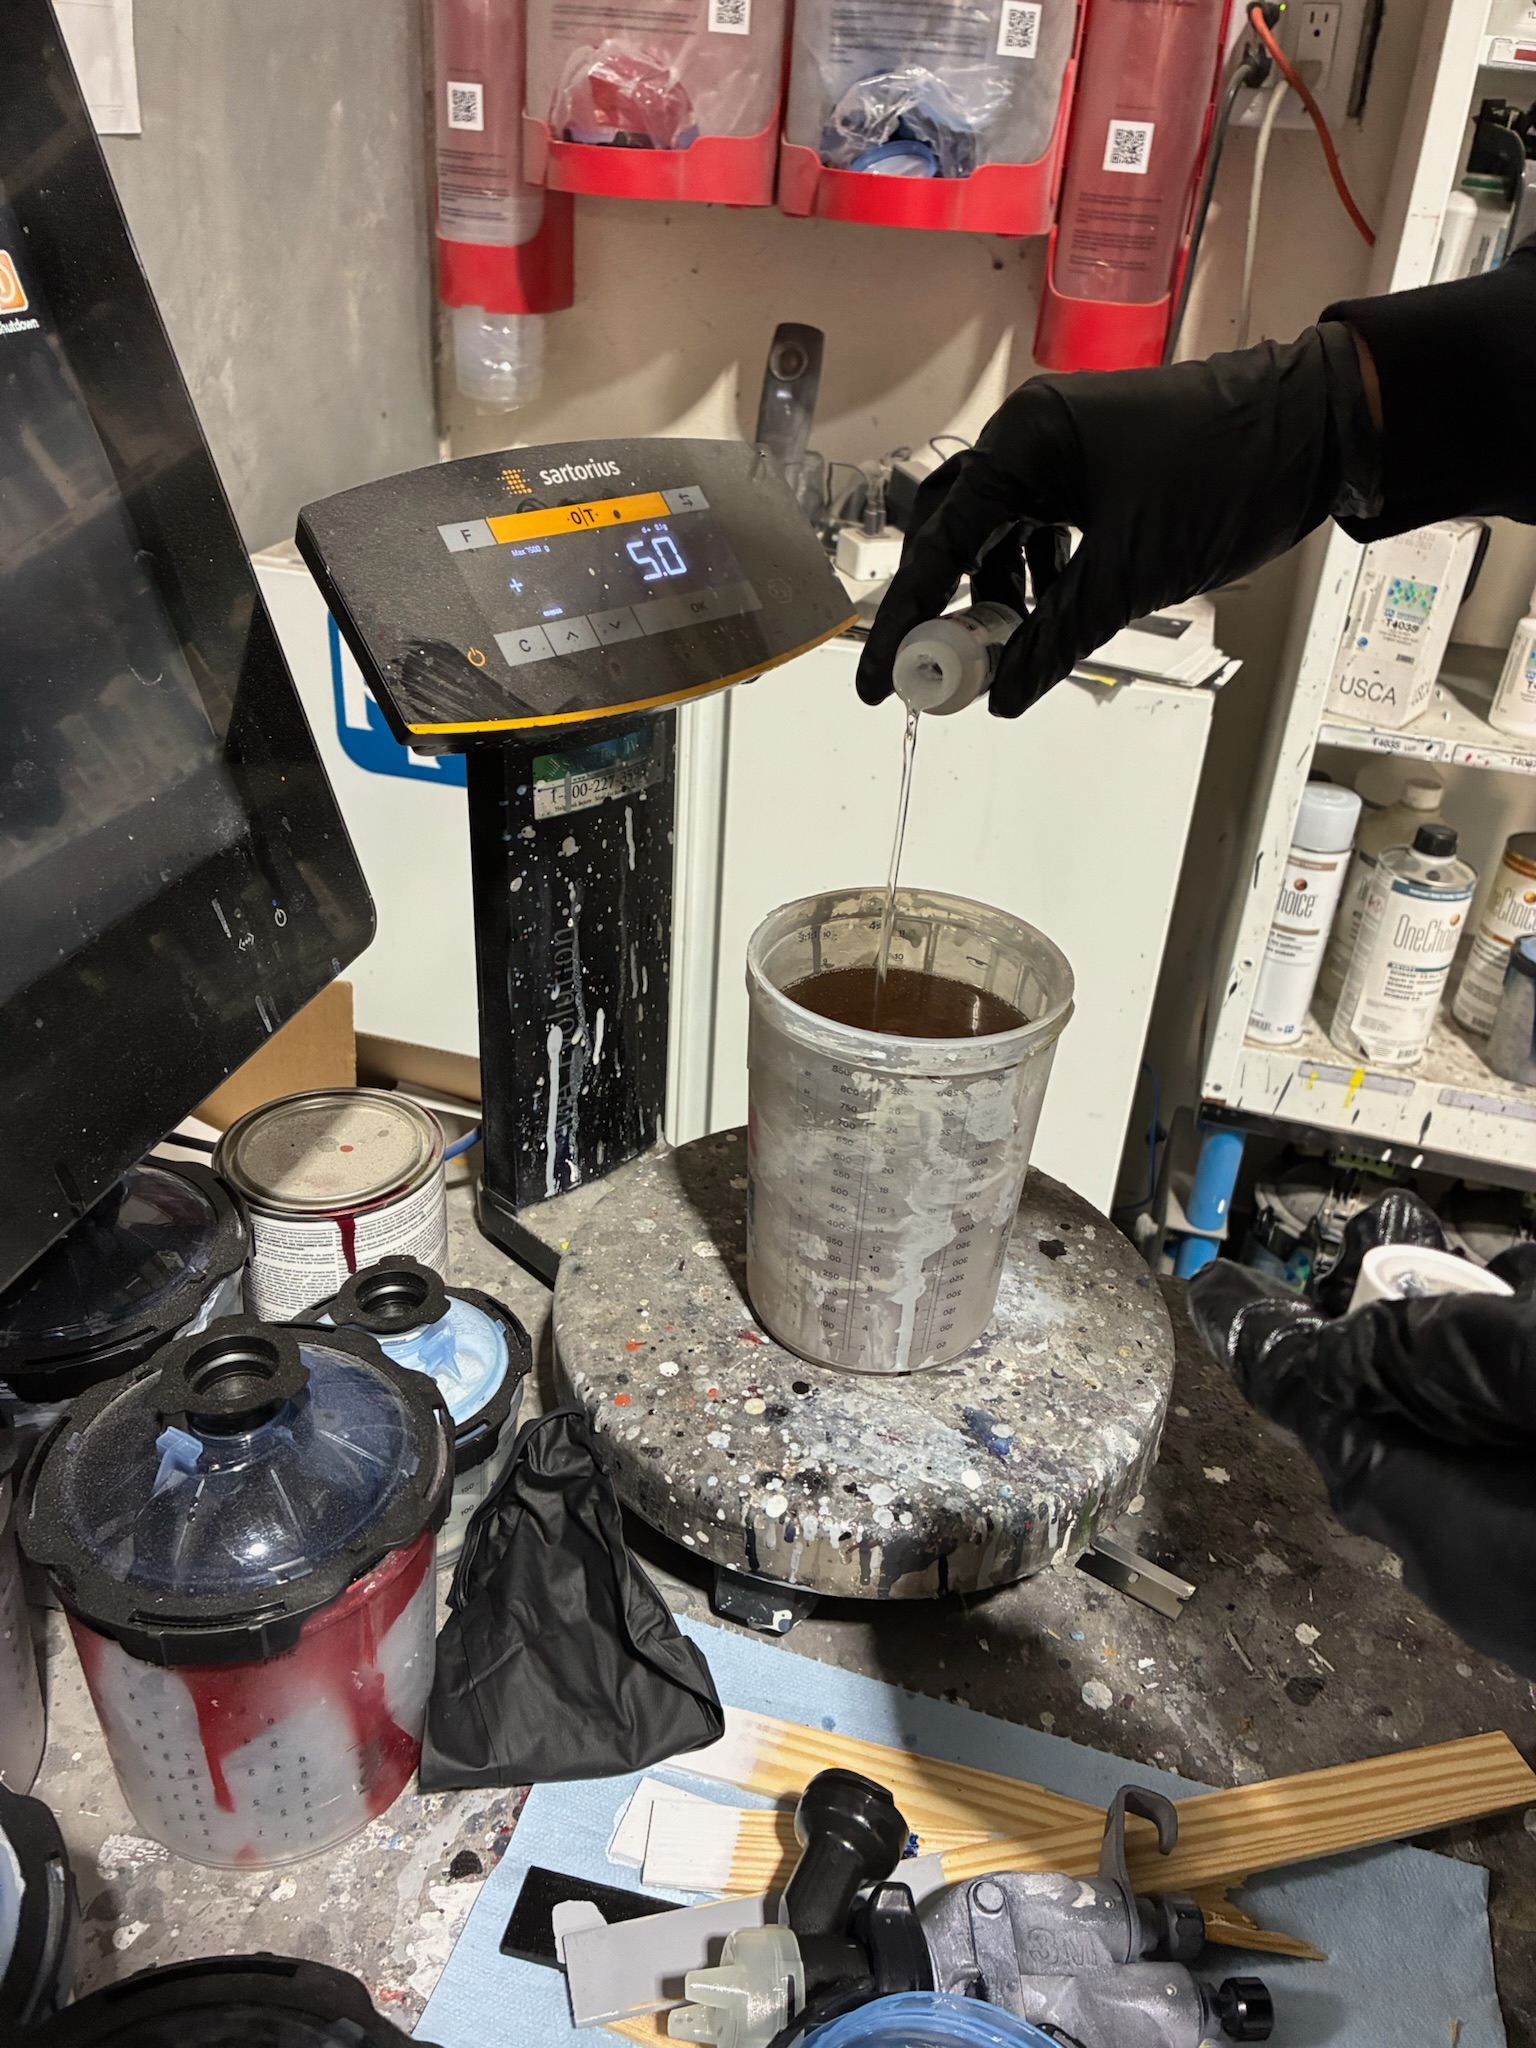
\includegraphics[
        width=2.35in,
        height=1.40in,
        keepaspectratio
    ]{spray_topcoat_prep}
};
\draw[RuleGray,line width=0.55pt,rounded corners=4pt]
    ($(current page.north west)+(0.43in,-1.91in)$)
    rectangle
    ($(current page.north west)+(2.98in,-3.40in)$);

% Image 2
\node[anchor=center,inner sep=0pt]
at ($(current page.north west)+(4.375in,-2.655in)$)
{
    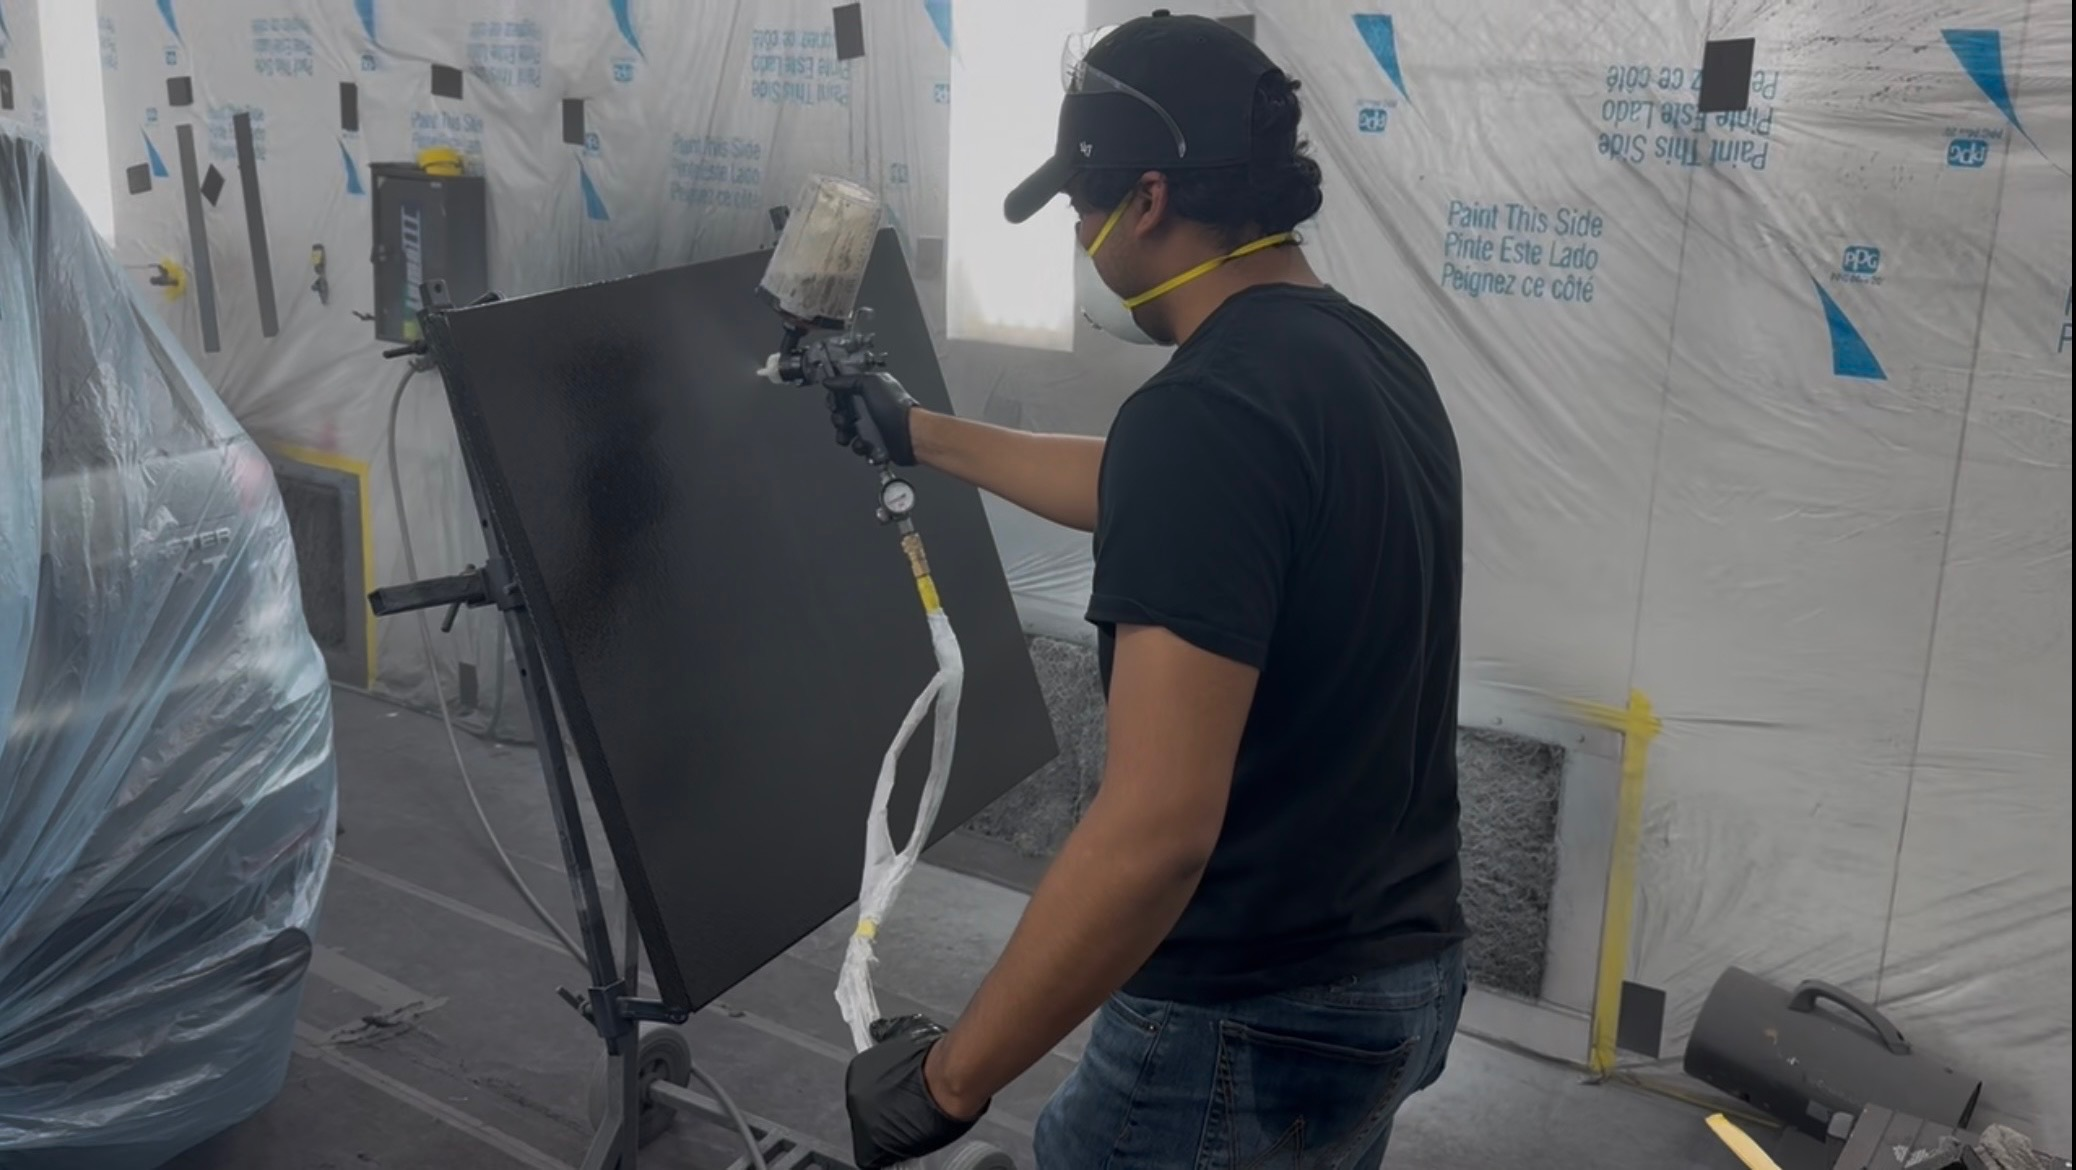
\includegraphics[
        width=2.35in,
        height=1.40in,
        keepaspectratio
    ]{spraying_topcoat}
};
\draw[RuleGray,line width=0.55pt,rounded corners=4pt]
    ($(current page.north west)+(3.10in,-1.91in)$)
    rectangle
    ($(current page.north west)+(5.65in,-3.40in)$);

% Image 3
\node[anchor=center,inner sep=0pt]
at ($(current page.north west)+(7.045in,-2.655in)$)
{
    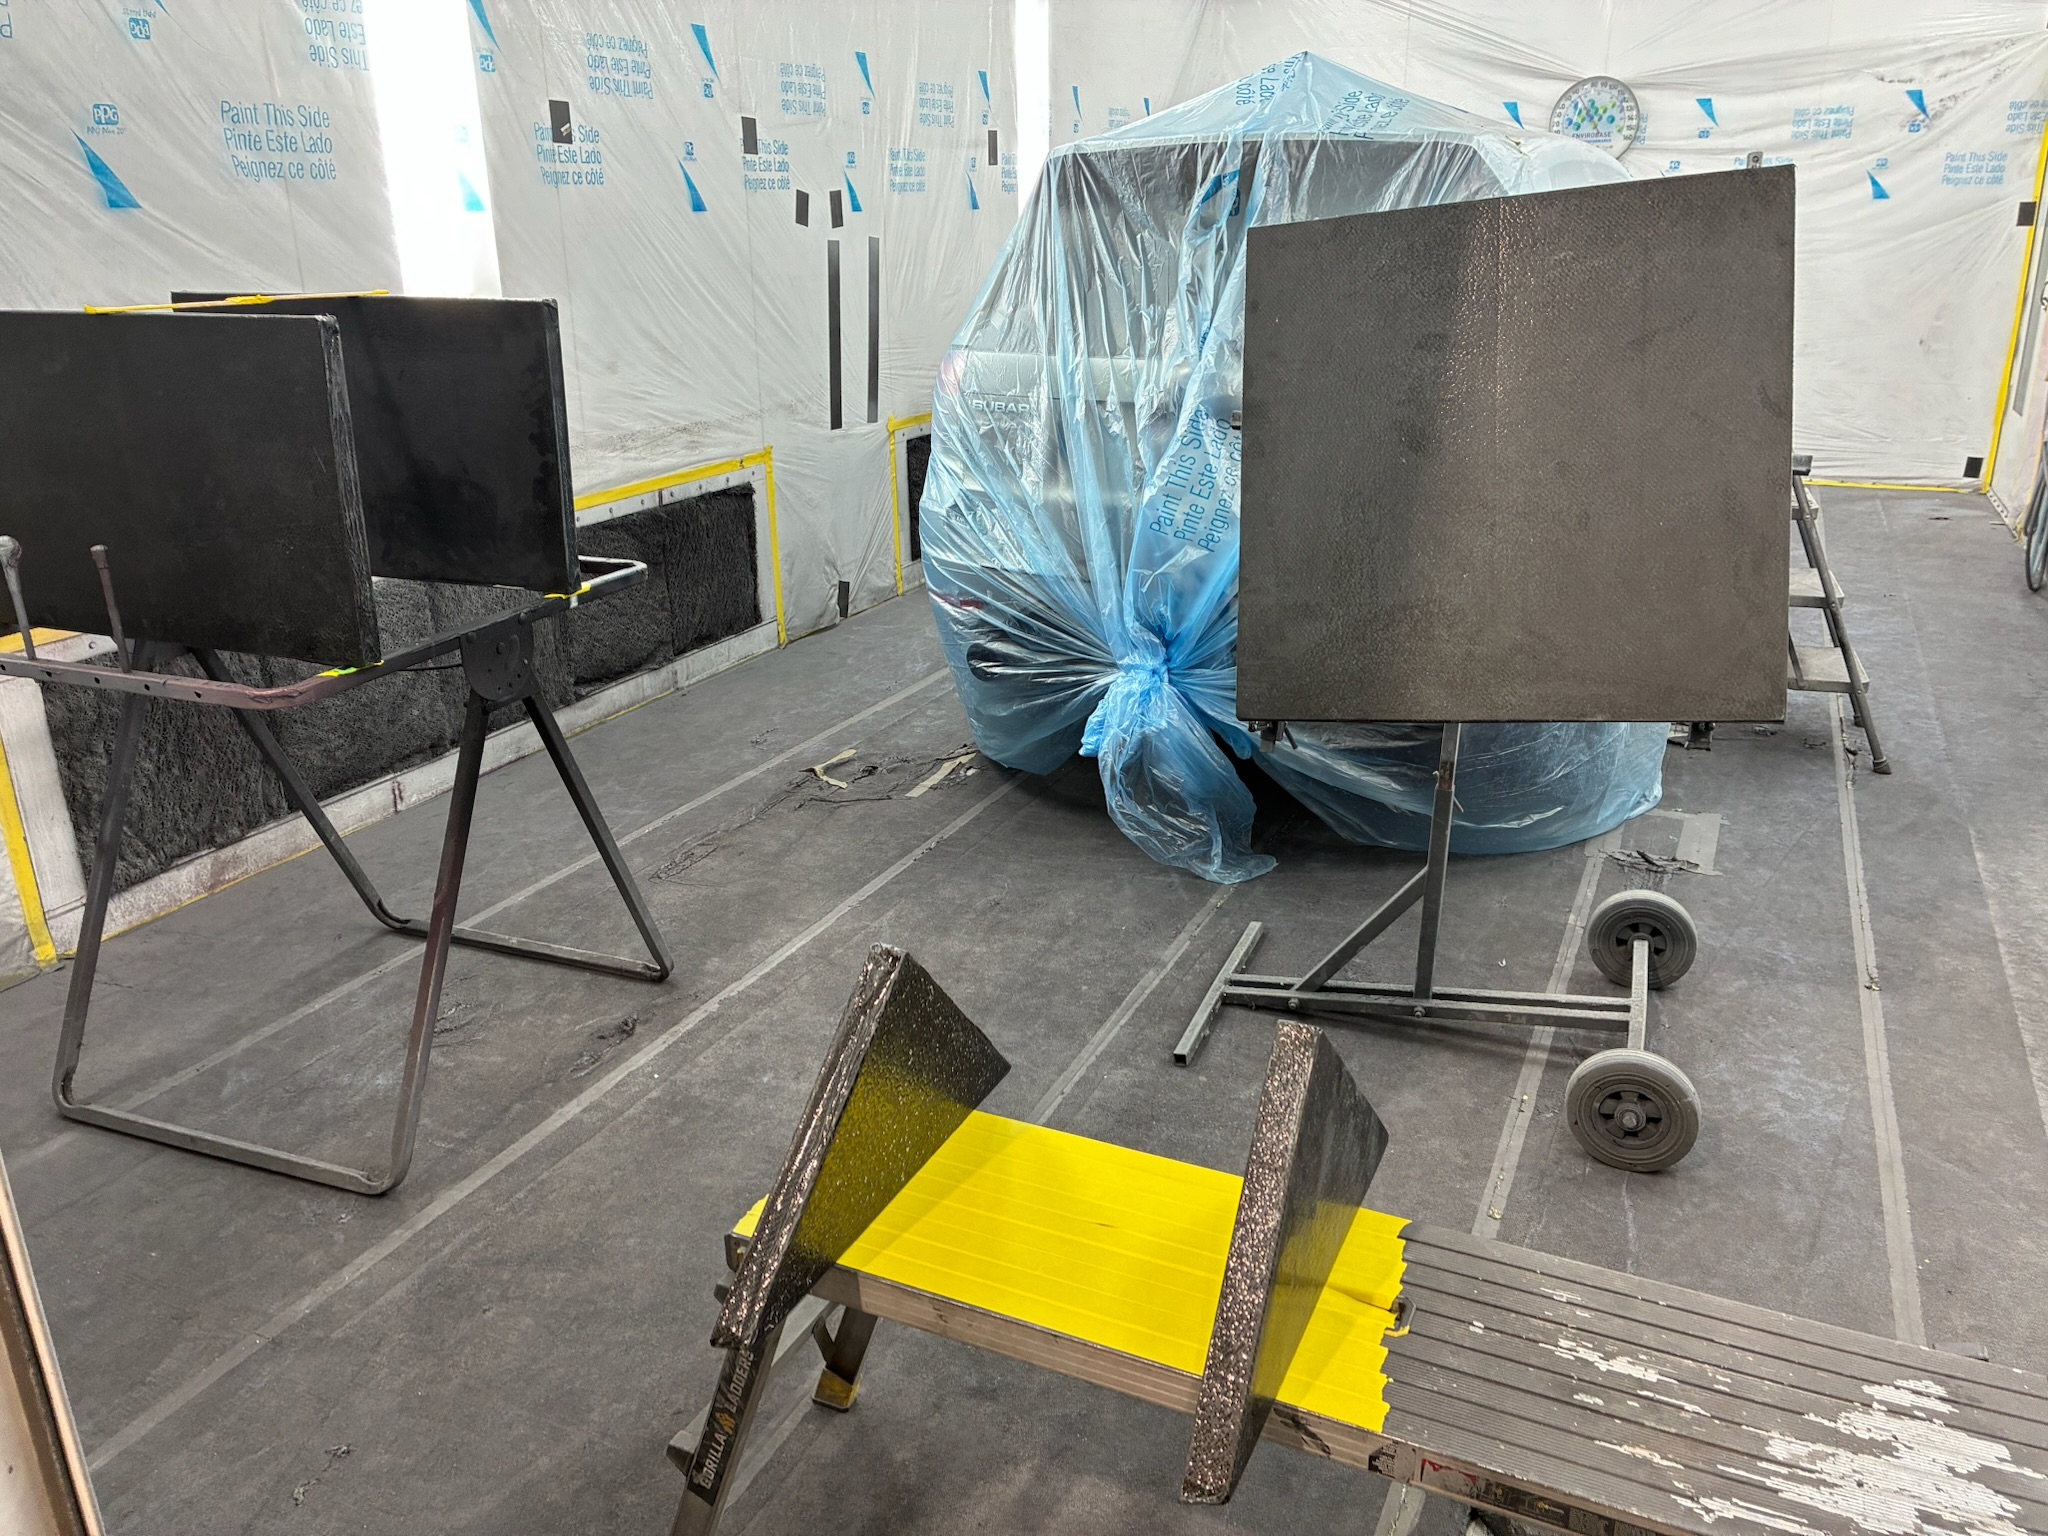
\includegraphics[
        width=2.35in,
        height=1.40in,
        keepaspectratio
    ]{topcoat_setup_apparatus}
};
\draw[RuleGray,line width=0.55pt,rounded corners=4pt]
    ($(current page.north west)+(5.77in,-1.91in)$)
    rectangle
    ($(current page.north west)+(8.32in,-3.40in)$);

% Image 4
\node[anchor=center,inner sep=0pt]
at ($(current page.north west)+(9.50in,-2.655in)$)
{
    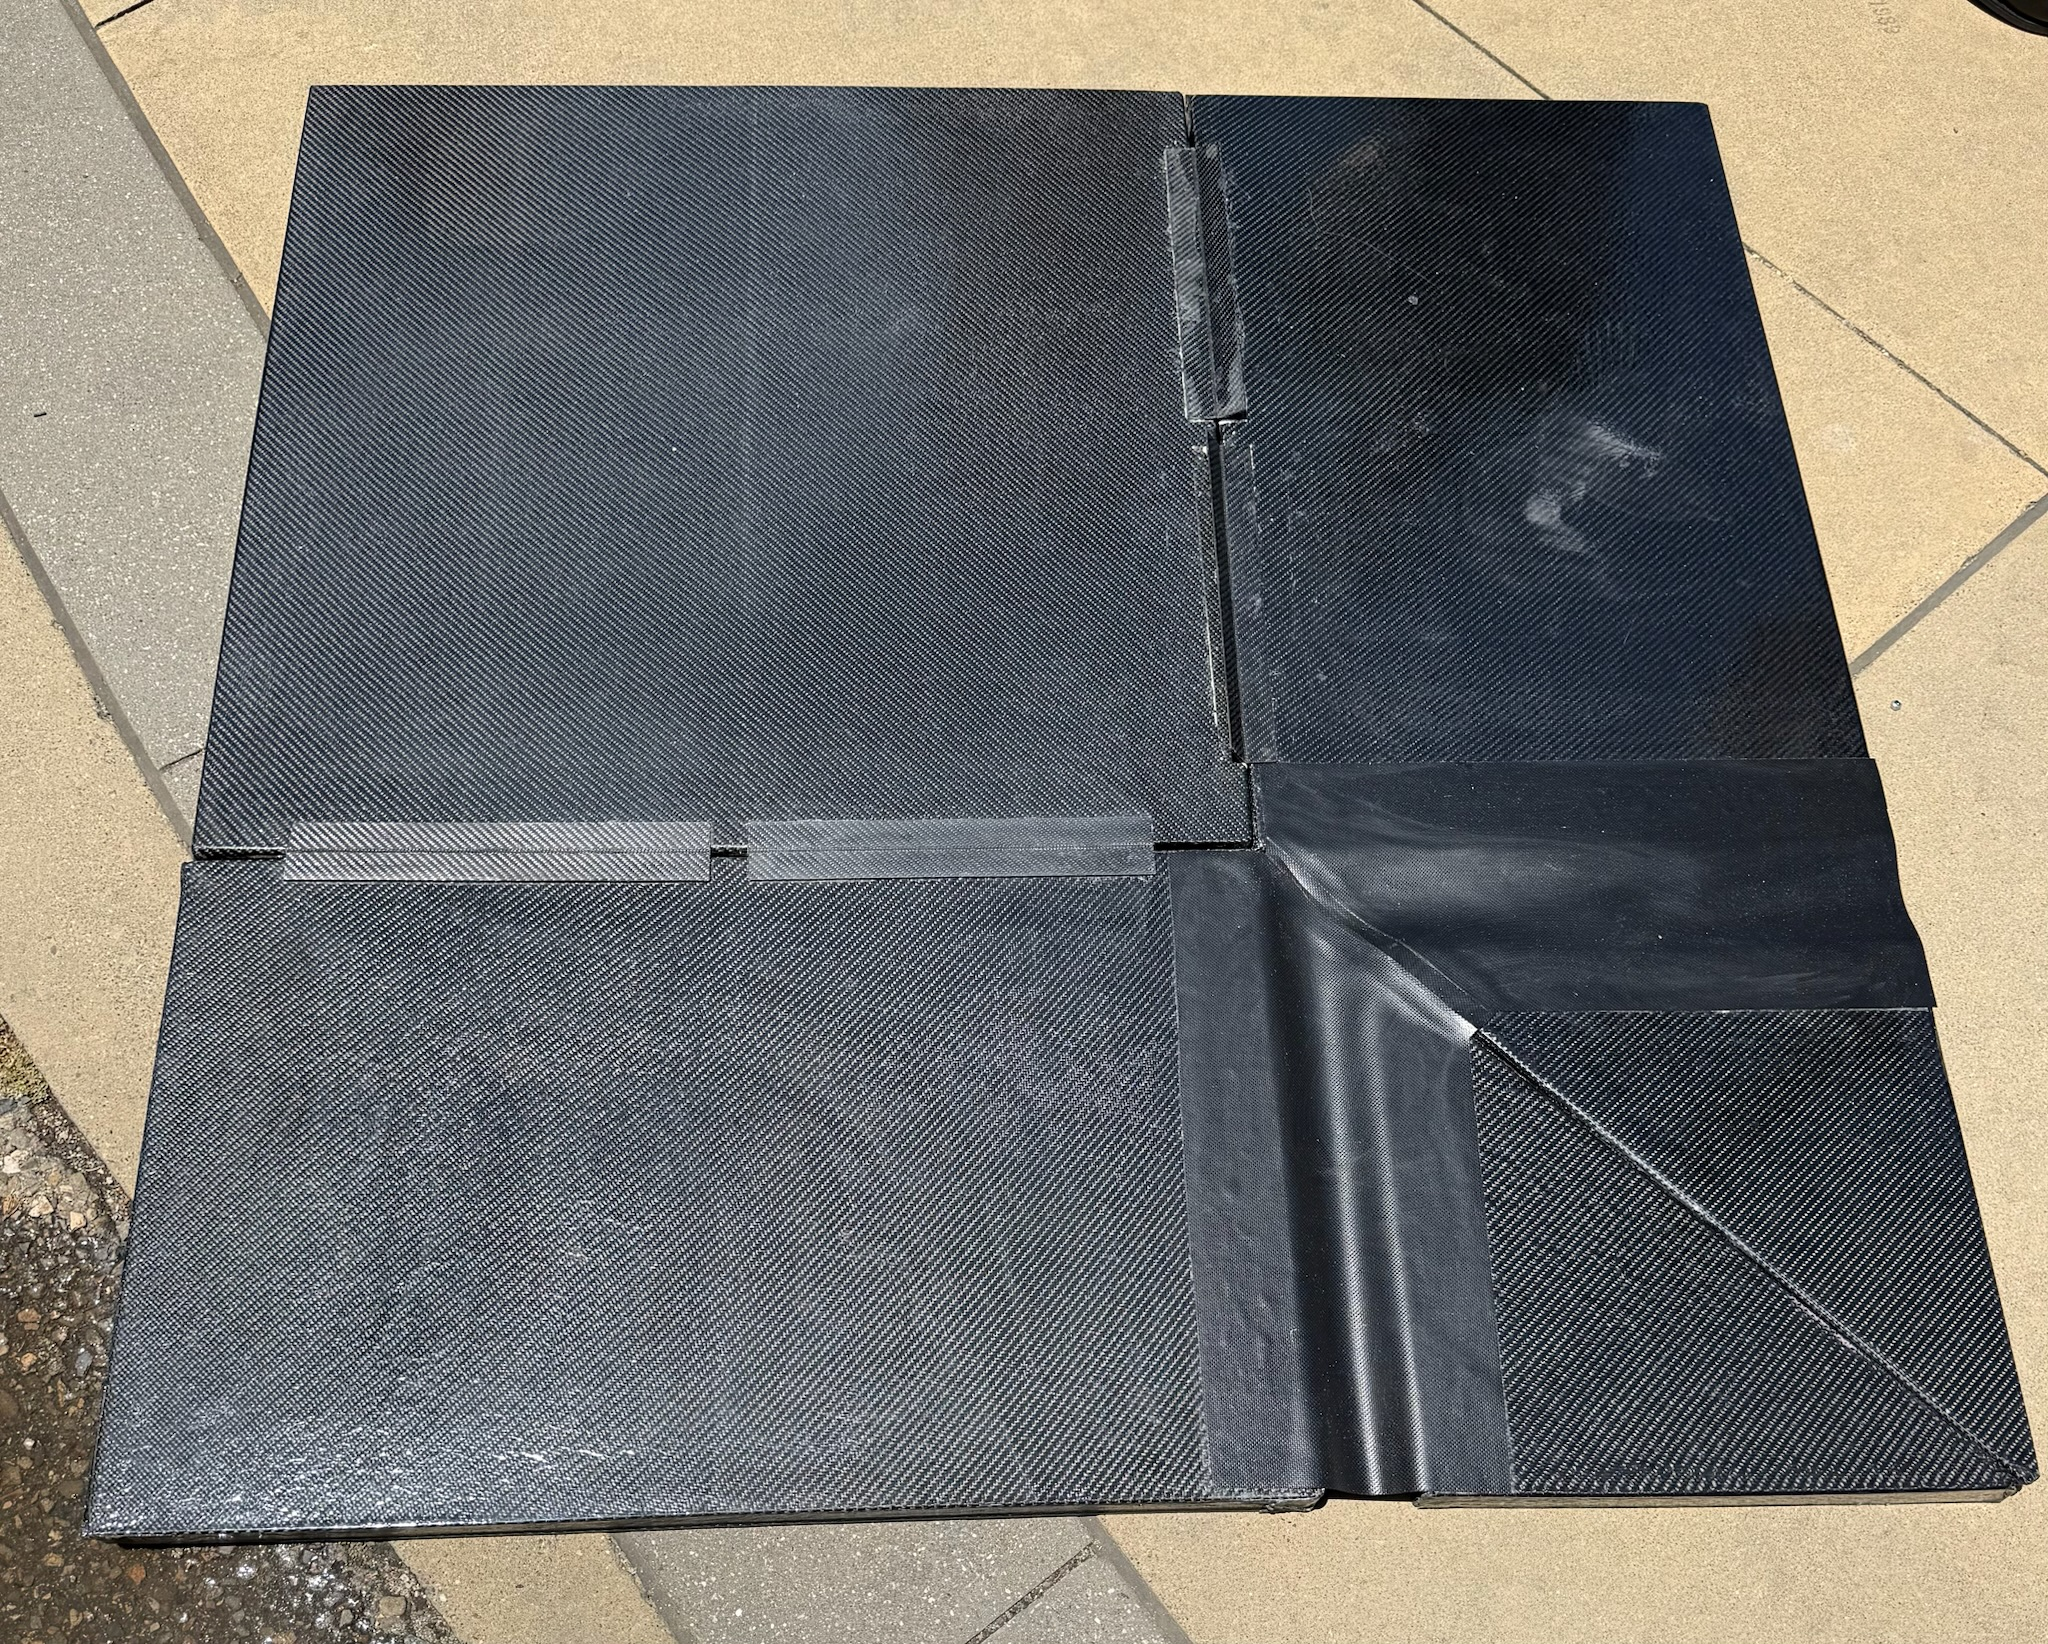
\includegraphics[
        width=2.35in,
        height=1.40in,
        keepaspectratio
    ]{refined_final_toro_cover_partial_carbon_model}
};
\draw[RuleGray,line width=0.55pt,rounded corners=4pt]
    ($(current page.north west)+(8.44in,-1.91in)$)
    rectangle
    ($(current page.north east)+(-0.42in,-3.40in)$);

% Captions
\node[anchor=north,text=Muted,font=\sffamily\fontsize{6.7}{7.3}\selectfont]
at ($(current page.north west)+(1.705in,-3.45in)$)
{Topcoat material preparation};

\node[anchor=north,text=Muted,font=\sffamily\fontsize{6.7}{7.3}\selectfont]
at ($(current page.north west)+(4.375in,-3.45in)$)
{Automotive-booth topcoat application};

\node[anchor=north,text=Muted,font=\sffamily\fontsize{6.7}{7.3}\selectfont]
at ($(current page.north west)+(7.045in,-3.45in)$)
{Coated panels drying after application};

\node[anchor=north,text=Muted,font=\sffamily\fontsize{6.7}{7.3}\selectfont]
at ($(current page.north west)+(9.50in,-3.45in)$)
{Partial carbon manufacturing model};

% Environmental rationale
\fill[SoftGold,rounded corners=4pt]
    ($(current page.north west)+(0.43in,-3.73in)$)
    rectangle
    ($(current page.north east)+(-0.42in,-4.76in)$);

\node[
    anchor=north west,
    align=left,
    text width=9.75in,
    text=Ink,
    font=\fontsize{7.05}{8.25}\selectfont
]
at ($(current page.north west)+(0.65in,-3.89in)$)
{
Because the sponsor required a carbon-fiber cover for outdoor use near chlorinated water,
environmental protection became a functional requirement rather than a cosmetic finish.
I selected and personally sprayed a UV-resistant Sunshield topcoat to seal minor laminate
porosity, reduce moisture ingress, preserve the carbon appearance, limit UV degradation of
the epoxy matrix, and isolate the composite surface from nearby metallic hardware.
};

% Results title
\node[
    anchor=north west,
    text=DeepGreen,
    font=\sffamily\bfseries\fontsize{8.0}{8.7}\selectfont
]
at ($(current page.north west)+(0.43in,-4.94in)$)
{FUNCTIONAL PROTOTYPE RESULTS};

% ------------------------------------------------------------
% Matched lower panels — larger type and improved allocation
% ------------------------------------------------------------

% Left results panel
\fill[SoftGreen,rounded corners=5pt]
    ($(current page.north west)+(0.43in,-5.22in)$)
    rectangle
    ($(current page.north west)+(5.98in,-7.39in)$);

\draw[RuleGray,line width=0.65pt,rounded corners=5pt]
    ($(current page.north west)+(0.43in,-5.22in)$)
    rectangle
    ($(current page.north west)+(5.98in,-7.39in)$);

\fill[DeepGreen,rounded corners=5pt]
    ($(current page.north west)+(0.43in,-5.22in)$)
    rectangle
    ($(current page.north west)+(5.98in,-5.58in)$);

\fill[DeepGreen]
    ($(current page.north west)+(0.43in,-5.40in)$)
    rectangle
    ($(current page.north west)+(5.98in,-5.58in)$);

\node[anchor=west,text=white,
      font=\sffamily\bfseries\fontsize{7.0}{7.6}\selectfont]
at ($(current page.north west)+(0.66in,-5.40in)$)
{SPECIFICATION};

\node[anchor=west,text=white,
      font=\sffamily\bfseries\fontsize{7.0}{7.6}\selectfont]
at ($(current page.north west)+(3.02in,-5.40in)$)
{RESULT};

\node[anchor=east,text=white,
      font=\sffamily\bfseries\fontsize{7.0}{7.6}\selectfont]
at ($(current page.north west)+(5.55in,-5.40in)$)
{STATUS};

\node[
    anchor=north west,
    align=left,
    text width=2.15in,
    text=Ink,
    font=\bfseries\fontsize{7.15}{8.55}\selectfont
]
at ($(current page.north west)+(0.66in,-5.72in)$)
{
Deployment time\\[3.4pt]
Removal time\\[3.4pt]
Single-user operation\\[3.4pt]
Single-side operation\\[3.4pt]
Deployment steps\\[3.4pt]
Removal steps\\[3.4pt]
Weight\\[3.4pt]
Folded storage
};

\node[
    anchor=north west,
    align=left,
    text width=1.45in,
    text=Ink,
    font=\fontsize{7.15}{8.55}\selectfont
]
at ($(current page.north west)+(3.02in,-5.72in)$)
{
25.51 seconds\\[3.4pt]
37.22 seconds\\[3.4pt]
100\% successful\\[3.4pt]
75\% successful\\[3.4pt]
6.4 average\\[3.4pt]
9 average\\[3.4pt]
17 lb\\[3.4pt]
2.9' x 2.9' x 1.7'
};

\node[
    anchor=north east,
    align=right,
    text width=1.05in,
    text=DeepGreen,
    font=\sffamily\bfseries\fontsize{7.05}{8.55}\selectfont
]
at ($(current page.north west)+(5.55in,-5.72in)$)
{
PASS\\[3.4pt]
PASS\\[3.4pt]
PASS\\[3.4pt]
NEAR TARGET\\[3.4pt]
PASS\\[3.4pt]
PASS\\[3.4pt]
NEAR TARGET\\[3.4pt]
PASS
};

% Right takeaways panel — widened for easier reading
\fill[SoftGreen,rounded corners=5pt]
    ($(current page.north west)+(6.14in,-5.22in)$)
    rectangle
    ($(current page.north east)+(-0.42in,-7.39in)$);

\draw[RuleGray,line width=0.65pt,rounded corners=5pt]
    ($(current page.north west)+(6.14in,-5.22in)$)
    rectangle
    ($(current page.north east)+(-0.42in,-7.39in)$);

\fill[DeepGreen,rounded corners=5pt]
    ($(current page.north west)+(6.14in,-5.22in)$)
    rectangle
    ($(current page.north east)+(-0.42in,-5.58in)$);

\fill[DeepGreen]
    ($(current page.north west)+(6.14in,-5.40in)$)
    rectangle
    ($(current page.north east)+(-0.42in,-5.58in)$);

\node[anchor=west,text=white,
      font=\sffamily\bfseries\fontsize{7.1}{7.7}\selectfont]
at ($(current page.north west)+(6.38in,-5.40in)$)
{ENGINEERING TAKEAWAYS};

\node[
    anchor=north west,
    align=left,
    text width=4.02in,
    text=Ink,
    font=\fontsize{6.75}{7.85}\selectfont
]
at ($(current page.north west)+(6.38in,-5.72in)$)
{
\textbf{Manufacturing first.}
Composite manufacturing constraints should guide the product architecture from the beginning.\\[4.5pt]
\textbf{Prioritize deliberately.}
Competing requirements must be balanced intentionally instead of maximizing every objective.\\[4.5pt]
\textbf{Lead through the process.}
Clear procedures, calm communication, and respect for teammates' strengths were essential during fabrication.\\[4.5pt]
\textbf{Next iteration.}
Reduce weight, refine the fabric-hinge fold lines, and improve panel-edge clearance.
};

% Compact concluding pathway
\node[
    anchor=center,
    align=center,
    text=PolyGold,
    font=\sffamily\bfseries\fontsize{6.3}{6.9}\selectfont
]
at ($(current page.north)+(3.06in,-7.18in)$)
{PROTOTYPE \faArrowRight\ DESIGN REFINEMENT
\faArrowRight\ REPEATABLE MANUFACTURING
\faArrowRight\ PRODUCT};

% Validation resources
\node[
    anchor=north,
    align=center,
    text=DeepGreen,
    font=\sffamily\bfseries\fontsize{6.6}{7.2}\selectfont
]
at ($(current page.north)+(0,-7.58in)$)
{\href{\ToroDeploymentLink}{\faPlayCircle\ DEPLOYMENT}
\hspace{18pt}
\href{\ToroRemovalLink}{\faPlayCircle\ REMOVAL / FOLDING}
\hspace{18pt}
\href{\ToroPosterLink}{\faFilePdf\ EXPO POSTER}
\hspace{18pt}
\href{\ToroReportLink}{\faFilePdf\ FINAL REPORT}};

% Footer
\node[
    anchor=south west,
    text=white,
    font=\sffamily\bfseries\fontsize{7.1}{7.7}\selectfont
]
at ($(current page.south west)+(0.42in,0.17in)$)
{\faArrowLeft\ MANUFACTURING-DRIVEN DESIGN};

\node[
    anchor=south,
    text=white,
    font=\sffamily\fontsize{7.0}{7.6}\selectfont
]
at ($(current page.south)+(0,0.17in)$)
{TORO COVER \hspace{6pt} 3 / 3};

\node[
    anchor=south east,
    text=white,
    font=\sffamily\bfseries\fontsize{7.1}{7.7}\selectfont
]
at ($(current page.south east)+(-0.42in,0.17in)$)
{NEXT PROJECT \faArrowRight};

\end{tikzpicture}
\input{paddle}
\clearpage
 before \end{document}.
% 3. Image references use the original Overleaf base filenames
%    without extensions.
% ============================================================



% ============================================================
% CLICKABLE PROJECT RESOURCES
% All links use the exact Google Drive resources supplied.
% ============================================================
\providecommand{\ToroDrawingLink}{https://drive.google.com/file/d/1A7-7wMnRNLuQDaTgxeuUCBsGNqyXzOGV/view?usp=sharing}
\providecommand{\ToroDimensionsLink}{https://drive.google.com/file/d/13sw3BNJvE8GdzlRffxoF2n5r9Gzxide7/view?usp=sharing}
\providecommand{\ToroProblemLink}{https://drive.google.com/file/d/1zHtl8zrb13F1yeN74ptawpfS5UM_xsuw/view?usp=drive_link}
\providecommand{\ToroReportLink}{https://drive.google.com/file/d/1ULZ-P46lFsC2x29ZfmRVIKgYnr9o8hMt/view?usp=drive_link}
\providecommand{\ToroPosterLink}{https://drive.google.com/file/d/1vKiKaJUcHQb_db-FkZnRF6EvtuM4hKyS/view?usp=drive_link}
\providecommand{\ToroDeploymentLink}{https://drive.google.com/file/d/1XJx34o80_mZPTl7xy93HtWAgtS3ThhvY/view?usp=drive_link}
\providecommand{\ToroRemovalLink}{https://drive.google.com/file/d/1O7xYeyB67NUwT-j1B1HeiCcHnZDYjk6_/view?usp=drive_link}

% ============================================================
% PAGE 1 — PROJECT OVERVIEW, OWNERSHIP, AND ARCHITECTURE
% ============================================================

\clearpage
\thispagestyle{empty}
\hypertarget{toro}{}
\null

\begin{tikzpicture}[remember picture,overlay]

% Background
\fill[white]
    (current page.south west)
    rectangle
    (current page.north east);

% Page bars
\fill[DeepGreen]
    (current page.north west)
    rectangle
    ($(current page.north east)+(0,-0.095in)$);

\fill[PolyGold]
    ($(current page.north west)+(0,-0.095in)$)
    rectangle
    ($(current page.north east)+(0,-0.14in)$);

\fill[DeepGreen]
    (current page.south west)
    rectangle
    ($(current page.south east)+(0,0.36in)$);

\fill[PolyGold]
    ($(current page.south west)+(0,0.36in)$)
    rectangle
    ($(current page.south east)+(0,0.405in)$);

% Header
\node[
    anchor=north west,
    text=PolyGold,
    font=\sffamily\bfseries\fontsize{8.1}{8.7}\selectfont
]
at ($(current page.north west)+(0.42in,-0.39in)$)
{01 COMPOSITES \hspace{5pt}/\hspace{5pt} PROJECT 01};

\node[
    anchor=north west,
    text=DeepGreen,
    font=\bfseries\fontsize{23.5}{24.5}\selectfont
]
at ($(current page.north west)+(0.40in,-0.67in)$)
{TORO CARBON FIBER SAFETY COVER};

\node[
    anchor=north west,
    text=Muted,
    font=\sffamily\fontsize{8.4}{9.2}\selectfont
]
at ($(current page.north west)+(0.42in,-1.12in)$)
{Cal Poly Composites Laboratory \hspace{7pt}\textbullet\hspace{7pt}
Team Project \hspace{7pt}\textbullet\hspace{7pt}
Fall--Spring 2026 \hspace{7pt}\textbullet\hspace{7pt}
San Luis Obispo, California};

\fill[PolyGold]
    ($(current page.north west)+(0.42in,-1.37in)$)
    rectangle
    ($(current page.north west)+(6.1in,-1.325in)$);

% Challenge text
\node[
    anchor=north west,
    text=DeepGreen,
    font=\sffamily\bfseries\fontsize{8.1}{8.8}\selectfont
]
at ($(current page.north west)+(0.43in,-1.61in)$)
{THE CHALLENGE};

\node[
    anchor=north west,
    align=left,
    text width=4.47in,
    text=Ink,
    font=\fontsize{8.05}{9.65}\selectfont
]
at ($(current page.north west)+(0.43in,-1.84in)$)
{
Develop a lightweight cover for a 6 ft by 6 ft in-ground spa
that could be deployed by one person, stored compactly,
provide insulation, resist a poolside environment, and maintain
a refined appearance. The sponsor supplied an ambitious but
intentionally broad project statement, requiring the team to
define the product architecture, priorities, manufacturing
strategy, and realistic path toward future commercialization.
};

% Role box
\fill[SoftGold,rounded corners=5pt]
    ($(current page.north west)+(0.42in,-2.88in)$)
    rectangle
    ($(current page.north west)+(4.98in,-4.58in)$);

\fill[PolyGold]
    ($(current page.north west)+(0.42in,-2.88in)$)
    rectangle
    ($(current page.north west)+(0.52in,-4.58in)$);

\node[
    anchor=north west,
    text=DeepGreen,
    font=\sffamily\bfseries\fontsize{8.1}{8.8}\selectfont
]
at ($(current page.north west)+(0.66in,-3.02in)$)
{MY ROLE — DESIGN \& MANUFACTURING LEAD};

\node[
    anchor=north west,
    align=left,
    text width=4.02in,
    text=Ink,
    font=\fontsize{7.05}{8.15}\selectfont
]
at ($(current page.north west)+(0.66in,-3.27in)$)
{
\textbullet\ Modeled every custom part and the complete assembly\\[1.5pt]
\textbullet\ Produced the engineering drawing package independently\\[1.5pt]
\textbullet\ Developed the composite-panel manufacturing process\\[1.5pt]
\textbullet\ Created all waterjet DXFs and manufacturing geometry\\[1.5pt]
\textbullet\ Trained teammates in wet layup and vacuum bagging\\[1.5pt]
\textbullet\ Presented feasibility, scope, and tradeoffs to the sponsor
};

% Large deployed foam-model image
\node[anchor=center,inner sep=0pt]
at ($(current page.north west)+(8.00in,-3.04in)$)
{
    \includegraphics[
        width=5.55in,
        height=2.78in,
        keepaspectratio
    ]{deployed_functional_prototype}
};

\draw[DeepGreen,line width=0.8pt,rounded corners=7pt]
    ($(current page.north west)+(5.16in,-1.61in)$)
    rectangle
    ($(current page.north east)+(-0.42in,-4.47in)$);

\node[
    anchor=north west,
    text=Muted,
    font=\sffamily\fontsize{6.2}{6.9}\selectfont
]
at ($(current page.north west)+(5.18in,-4.54in)$)
{Functional foam model deployed over the sponsor's in-ground spa.};

% Image-strip title
\node[
    anchor=north west,
    text=DeepGreen,
    font=\sffamily\bfseries\fontsize{8.1}{8.8}\selectfont
]
at ($(current page.north west)+(0.43in,-4.78in)$)
{PRODUCT DEVELOPMENT AND FINAL ARCHITECTURE};

% Five-image development strip — CAD-first sequence
% Image 1: topside CAD
\node[anchor=center,inner sep=0pt]
at ($(current page.north west)+(1.47in,-5.73in)$)
{
    \includegraphics[
        width=1.92in,
        height=1.30in,
        keepaspectratio
    ]{Toro_Cover_topside_Cad}
};
\draw[RuleGray,line width=0.55pt,rounded corners=4pt]
    ($(current page.north west)+(0.43in,-5.04in)$)
    rectangle
    ($(current page.north west)+(2.51in,-6.43in)$);

% Image 2: underside CAD
\node[anchor=center,inner sep=0pt]
at ($(current page.north west)+(3.66in,-5.73in)$)
{
    \includegraphics[
        width=1.92in,
        height=1.30in,
        keepaspectratio
    ]{toro_cover_underside_cad}
};
\draw[RuleGray,line width=0.55pt,rounded corners=4pt]
    ($(current page.north west)+(2.62in,-5.04in)$)
    rectangle
    ($(current page.north west)+(4.70in,-6.43in)$);

% Image 3: folded CAD
\node[anchor=center,inner sep=0pt]
at ($(current page.north west)+(5.85in,-5.73in)$)
{
    \includegraphics[
        width=1.92in,
        height=1.30in,
        keepaspectratio
    ]{\detokenize{Toro_Cover_folded Configuration}}
};
\draw[RuleGray,line width=0.55pt,rounded corners=4pt]
    ($(current page.north west)+(4.81in,-5.04in)$)
    rectangle
    ($(current page.north west)+(6.89in,-6.43in)$);

% Image 4: dual-use product concept
\node[anchor=center,inner sep=0pt]
at ($(current page.north west)+(8.04in,-5.73in)$)
{
    \includegraphics[
        width=1.92in,
        height=1.30in,
        keepaspectratio
    ]{generative_AI_concept_toro_cover_art}
};
\draw[RuleGray,line width=0.55pt,rounded corners=4pt]
    ($(current page.north west)+(7.00in,-5.04in)$)
    rectangle
    ($(current page.north west)+(9.08in,-6.43in)$);

% Image 5: folded foam functional prototype
% The portrait photograph is deliberately clipped to the landscape frame
% so the ottoman fills the card without extending beyond its border.
\begin{scope}
\clip[rounded corners=4pt]
    ($(current page.north west)+(9.19in,-5.04in)$)
    rectangle
    ($(current page.north east)+(-0.43in,-6.43in)$);

% Keep the original image proportions and center it within the existing card.
\node[anchor=center,inner sep=0pt]
at ($(current page.north west)+(9.88in,-5.735in)$)
{
    \includegraphics[
        width=1.58in,
        height=1.28in,
        keepaspectratio
    ]{foam_model_folded_backyard_image}
};
\end{scope}

\draw[RuleGray,line width=0.55pt,rounded corners=4pt]
    ($(current page.north west)+(9.19in,-5.04in)$)
    rectangle
    ($(current page.north east)+(-0.43in,-6.43in)$);

% Larger captions
\node[anchor=north,align=center,text width=1.95in,text=Muted,
      font=\sffamily\fontsize{6.8}{7.4}\selectfont]
at ($(current page.north west)+(1.47in,-6.49in)$)
{Topside panel architecture};

\node[anchor=north,align=center,text width=1.95in,text=Muted,
      font=\sffamily\fontsize{6.8}{7.4}\selectfont]
at ($(current page.north west)+(3.66in,-6.49in)$)
{Underside hinge architecture};

\node[anchor=north,align=center,text width=1.95in,text=Muted,
      font=\sffamily\fontsize{6.8}{7.4}\selectfont]
at ($(current page.north west)+(5.85in,-6.49in)$)
{Folded CAD configuration};

\node[anchor=north,align=center,text width=1.95in,text=Muted,
      font=\sffamily\fontsize{6.8}{7.4}\selectfont]
at ($(current page.north west)+(8.04in,-6.49in)$)
{Dual-use product vision};

\node[anchor=north,align=center,text width=1.95in,text=Muted,
      font=\sffamily\fontsize{6.8}{7.4}\selectfont]
at ($(current page.north west)+(9.88in,-6.49in)$)
{Folded foam prototype};

% Page 1 resource bar — centered and non-repeated resources
\fill[Panel,rounded corners=4pt]
    ($(current page.north west)+(0.43in,-7.05in)$)
    rectangle
    ($(current page.north east)+(-0.43in,-7.64in)$);
\draw[RuleGray,line width=0.5pt,rounded corners=4pt]
    ($(current page.north west)+(0.43in,-7.05in)$)
    rectangle
    ($(current page.north east)+(-0.43in,-7.64in)$);

\node[
    anchor=center,
    align=center,
    text=DeepGreen,
    font=\sffamily\bfseries\fontsize{6.9}{7.5}\selectfont
]
at ($(current page.north)+(0,-7.345in)$)
{\href{\ToroDrawingLink}{\faDraftingCompass\ DRAWING PACKAGE}
\hspace{24pt}
\href{\ToroDimensionsLink}{\faImage\ DIMENSION STUDY}
\hspace{24pt}
\href{\ToroProblemLink}{\faFileImage\ PROBLEM STATEMENT}};

% Footer
\node[
    anchor=south west,
    text=white,
    font=\sffamily\bfseries\fontsize{7.1}{7.7}\selectfont
]
at ($(current page.south west)+(0.42in,0.17in)$)
{\hyperlink{composites}{\faArrowLeft\ COMPOSITES}};

\node[
    anchor=south,
    text=white,
    font=\sffamily\fontsize{7.0}{7.6}\selectfont
]
at ($(current page.south)+(0,0.17in)$)
{TORO COVER \hspace{6pt} 1 / 3};

\node[
    anchor=south east,
    text=white,
    font=\sffamily\bfseries\fontsize{7.1}{7.7}\selectfont
]
at ($(current page.south east)+(-0.42in,0.17in)$)
{MANUFACTURING-DRIVEN DESIGN \faArrowRight};

\end{tikzpicture}


% ============================================================
% PAGE 2 — MANUFACTURING-DRIVEN DESIGN
% ============================================================

\clearpage
\thispagestyle{empty}
\hypertarget{toro-manufacturing}{}
\null

\begin{tikzpicture}[remember picture,overlay]

% Background and bars
\fill[white]
    (current page.south west)
    rectangle
    (current page.north east);

\fill[DeepGreen]
    (current page.north west)
    rectangle
    ($(current page.north east)+(0,-0.095in)$);

\fill[PolyGold]
    ($(current page.north west)+(0,-0.095in)$)
    rectangle
    ($(current page.north east)+(0,-0.14in)$);

\fill[DeepGreen]
    (current page.south west)
    rectangle
    ($(current page.south east)+(0,0.36in)$);

\fill[PolyGold]
    ($(current page.south west)+(0,0.36in)$)
    rectangle
    ($(current page.south east)+(0,0.405in)$);

% Header
\node[
    anchor=north west,
    text=PolyGold,
    font=\sffamily\bfseries\fontsize{8.1}{8.7}\selectfont
]
at ($(current page.north west)+(0.42in,-0.39in)$)
{TORO COVER \hspace{5pt}/\hspace{5pt} DESIGN FOR MANUFACTURABILITY};

\node[
    anchor=north west,
    text=DeepGreen,
    font=\bfseries\fontsize{23}{24}\selectfont
]
at ($(current page.north west)+(0.40in,-0.67in)$)
{THE ENVELOPE METHOD};

\node[
    anchor=north west,
    text=Muted,
    font=\sffamily\fontsize{8.7}{9.6}\selectfont
]
at ($(current page.north west)+(0.42in,-1.12in)$)
{A one-layup process developed for unusually thick insulated composite sandwich panels};

\fill[PolyGold]
    ($(current page.north west)+(0.42in,-1.36in)$)
    rectangle
    ($(current page.north west)+(5.30in,-1.315in)$);

% Process explanation
\fill[SoftGold,rounded corners=5pt]
    ($(current page.north west)+(0.42in,-1.61in)$)
    rectangle
    ($(current page.north east)+(-0.42in,-2.90in)$);

\fill[PolyGold]
    ($(current page.north west)+(0.42in,-1.61in)$)
    rectangle
    ($(current page.north west)+(0.52in,-2.90in)$);

\node[
    anchor=north west,
    text=DeepGreen,
    font=\sffamily\bfseries\fontsize{7.9}{8.6}\selectfont
]
at ($(current page.north west)+(0.67in,-1.76in)$)
{PROCESS INNOVATION};

\node[
    anchor=north west,
    align=left,
    text width=9.55in,
    text=Ink,
    font=\fontsize{7.35}{8.75}\selectfont
]
at ($(current page.north west)+(0.67in,-2.02in)$)
{
Weight reduction and insulation were both essential, leading to the selection of an
XPS foam core. Because XPS could not tolerate composite heat-cure temperatures, prepreg
processing was not practical and the panels had to be manufactured by wet layup with a
room-temperature cure. To simplify this process, I waterjet-cut XPS perimeter strips from
excess foam and placed them around each core inside the vacuum enclosure. Under vacuum,
the top and bottom carbon skins met along the panel sides and compressed against this
border, eliminating a separate edge-banding layup and reducing corner pleating.
};

% Workflow title
\node[
    anchor=north west,
    text=DeepGreen,
    font=\sffamily\bfseries\fontsize{8.0}{8.7}\selectfont
]
at ($(current page.north west)+(0.43in,-3.06in)$)
{MANUFACTURING WORKFLOW};

% Row 1 image 1
\node[anchor=center,inner sep=0pt]
at ($(current page.north west)+(2.07in,-4.105in)$)
{
    \includegraphics[
        width=3.10in,
        height=1.40in,
        keepaspectratio
    ]{waterjet_foam}
};
\draw[RuleGray,line width=0.55pt,rounded corners=4pt]
    ($(current page.north west)+(0.43in,-3.36in)$)
    rectangle
    ($(current page.north west)+(3.71in,-4.85in)$);

% Row 1 image 2
\node[anchor=center,inner sep=0pt]
at ($(current page.north west)+(5.50in,-4.105in)$)
{
    \includegraphics[
        width=3.10in,
        height=1.40in,
        keepaspectratio
    ]{group_layup}
};
\draw[RuleGray,line width=0.55pt,rounded corners=4pt]
    ($(current page.north west)+(3.86in,-3.36in)$)
    rectangle
    ($(current page.north west)+(7.14in,-4.85in)$);

% Row 1 image 3
\node[anchor=center,inner sep=0pt]
at ($(current page.north west)+(8.935in,-4.105in)$)
{
    \includegraphics[
        width=3.10in,
        height=1.40in,
        keepaspectratio
    ]{blue_perforrated_film_layup}
};
\draw[RuleGray,line width=0.55pt,rounded corners=4pt]
    ($(current page.north west)+(7.29in,-3.36in)$)
    rectangle
    ($(current page.north east)+(-0.42in,-4.85in)$);

% Row 1 captions
\node[anchor=north,text=Muted,font=\sffamily\fontsize{6.7}{7.3}\selectfont]
at ($(current page.north west)+(2.07in,-4.90in)$)
{1. Waterjet-cut core and perimeter geometry};

\node[anchor=north,text=Muted,font=\sffamily\fontsize{6.7}{7.3}\selectfont]
at ($(current page.north west)+(5.50in,-4.90in)$)
{2. Team wet layup under my process guidance};

\node[anchor=north,text=Muted,font=\sffamily\fontsize{6.7}{7.3}\selectfont]
at ($(current page.north west)+(8.935in,-4.90in)$)
{3. Perforated film, breather, and vacuum enclosure};

% Row 2 image 1
\node[anchor=center,inner sep=0pt]
at ($(current page.north west)+(2.07in,-5.875in)$)
{
    \includegraphics[
        width=3.10in,
        height=1.40in,
        keepaspectratio
    ]{completed_layup}
};
\draw[RuleGray,line width=0.55pt,rounded corners=4pt]
    ($(current page.north west)+(0.43in,-5.13in)$)
    rectangle
    ($(current page.north west)+(3.71in,-6.62in)$);

% Row 2 image 2 — oven chamber used only as a reliable vacuum enclosure; no heat applied
\node[anchor=center,inner sep=0pt]
at ($(current page.north west)+(5.50in,-5.875in)$)
{
    \includegraphics[
        width=3.10in,
        height=1.40in,
        keepaspectratio
    ]{layups_in_composite_oven_under_vacuumPressure}
};
\draw[RuleGray,line width=0.55pt,rounded corners=4pt]
    ($(current page.north west)+(3.86in,-5.13in)$)
    rectangle
    ($(current page.north west)+(7.14in,-6.62in)$);

% Row 2 image 3
\node[anchor=center,inner sep=0pt]
at ($(current page.north west)+(8.935in,-5.875in)$)
{
    \includegraphics[
        width=3.10in,
        height=1.40in,
        keepaspectratio
    ]{garage_sanding}
};
\draw[RuleGray,line width=0.55pt,rounded corners=4pt]
    ($(current page.north west)+(7.29in,-5.13in)$)
    rectangle
    ($(current page.north east)+(-0.42in,-6.62in)$);

% Row 2 captions
\node[anchor=north,text=Muted,font=\sffamily\fontsize{6.7}{7.3}\selectfont]
at ($(current page.north west)+(2.07in,-6.67in)$)
{4. Fully saturated carbon skin and foam sandwich};

\node[anchor=north,text=Muted,font=\sffamily\fontsize{6.7}{7.3}\selectfont]
at ($(current page.north west)+(5.50in,-6.67in)$)
{5. Room-temperature cure under continuous vacuum};

\node[anchor=north,text=Muted,font=\sffamily\fontsize{6.7}{7.3}\selectfont]
at ($(current page.north west)+(8.935in,-6.67in)$)
{6. Post-processing and surface preparation};

% Bottom callouts
\fill[Panel,rounded corners=4pt]
    ($(current page.north west)+(0.43in,-6.95in)$)
    rectangle
    ($(current page.north west)+(5.48in,-7.60in)$);

\draw[RuleGray,line width=0.55pt,rounded corners=4pt]
    ($(current page.north west)+(0.43in,-6.95in)$)
    rectangle
    ($(current page.north west)+(5.48in,-7.60in)$);

\node[
    anchor=north west,
    text=DeepGreen,
    font=\sffamily\bfseries\fontsize{7.0}{7.6}\selectfont
]
at ($(current page.north west)+(0.63in,-7.08in)$)
{FROM THREE LAYUPS TO ONE};

\node[
    anchor=north west,
    align=left,
    text width=4.56in,
    text=Ink,
    font=\fontsize{6.45}{7.45}\selectfont
]
at ($(current page.north west)+(0.63in,-7.29in)$)
{
The Envelope Method reduced labor, cure cycles, handling,
alignment risk, and time spent forming numerous vacuum-bag
pleats around the 1.5-inch-thick XPS panels.
};

\fill[Panel,rounded corners=4pt]
    ($(current page.north west)+(5.68in,-6.95in)$)
    rectangle
    ($(current page.north east)+(-0.42in,-7.60in)$);

\draw[RuleGray,line width=0.55pt,rounded corners=4pt]
    ($(current page.north west)+(5.68in,-6.95in)$)
    rectangle
    ($(current page.north east)+(-0.42in,-7.60in)$);

\node[
    anchor=north west,
    text=DeepGreen,
    font=\sffamily\bfseries\fontsize{7.0}{7.6}\selectfont
]
at ($(current page.north west)+(5.88in,-7.08in)$)
{WHY SURFACE-BONDED HARDWARE};

\node[
    anchor=north west,
    align=left,
    text width=4.55in,
    text=Ink,
    font=\fontsize{6.45}{7.45}\selectfont
]
at ($(current page.north west)+(5.88in,-7.29in)$)
{
Adhesively bonded hinges and fixtures preserved the clean
composite exterior and avoided drilled inserts, foam-core
crushing, added stress concentrations, and new leak paths.
};


% Footer
\node[
    anchor=south west,
    text=white,
    font=\sffamily\bfseries\fontsize{7.1}{7.7}\selectfont
]
at ($(current page.south west)+(0.42in,0.17in)$)
{\faArrowLeft\ PRODUCT ARCHITECTURE};

\node[
    anchor=south,
    text=white,
    font=\sffamily\fontsize{7.0}{7.6}\selectfont
]
at ($(current page.south)+(0,0.17in)$)
{TORO COVER \hspace{6pt} 2 / 3};

\node[
    anchor=south east,
    text=white,
    font=\sffamily\bfseries\fontsize{7.1}{7.7}\selectfont
]
at ($(current page.south east)+(-0.42in,0.17in)$)
{VALIDATION \& TAKEAWAYS \faArrowRight};

\end{tikzpicture}


% ============================================================
% PAGE 3 — FINISHING, VALIDATION, AND TAKEAWAYS
% ============================================================

\clearpage
\thispagestyle{empty}
\hypertarget{toro-results}{}
\null

\begin{tikzpicture}[remember picture,overlay]

% Background and bars
\fill[white]
    (current page.south west)
    rectangle
    (current page.north east);

\fill[DeepGreen]
    (current page.north west)
    rectangle
    ($(current page.north east)+(0,-0.095in)$);

\fill[PolyGold]
    ($(current page.north west)+(0,-0.095in)$)
    rectangle
    ($(current page.north east)+(0,-0.14in)$);

\fill[DeepGreen]
    (current page.south west)
    rectangle
    ($(current page.south east)+(0,0.36in)$);

\fill[PolyGold]
    ($(current page.south west)+(0,0.36in)$)
    rectangle
    ($(current page.south east)+(0,0.405in)$);

% Header
\node[
    anchor=north west,
    text=PolyGold,
    font=\sffamily\bfseries\fontsize{8.1}{8.7}\selectfont
]
at ($(current page.north west)+(0.42in,-0.39in)$)
{TORO COVER \hspace{5pt}/\hspace{5pt} VALIDATION AND ENGINEERING TAKEAWAYS};

\node[
    anchor=north west,
    text=DeepGreen,
    font=\bfseries\fontsize{22.5}{23.5}\selectfont
]
at ($(current page.north west)+(0.40in,-0.67in)$)
{FROM PROTOTYPE TO PRODUCT PATHWAY};

\node[
    anchor=north west,
    text=Muted,
    font=\sffamily\fontsize{8.7}{9.6}\selectfont
]
at ($(current page.north west)+(0.42in,-1.12in)$)
{Environmental protection, usability testing, scope decisions, and lessons from technical leadership};

\fill[PolyGold]
    ($(current page.north west)+(0.42in,-1.36in)$)
    rectangle
    ($(current page.north west)+(5.8in,-1.315in)$);

% Finishing title
\node[
    anchor=north west,
    text=DeepGreen,
    font=\sffamily\bfseries\fontsize{8.0}{8.7}\selectfont
]
at ($(current page.north west)+(0.43in,-1.62in)$)
{OUTDOOR FINISHING AND ENVIRONMENTAL PROTECTION};

% Image 1
\node[anchor=center,inner sep=0pt]
at ($(current page.north west)+(1.705in,-2.655in)$)
{
    \includegraphics[
        width=2.35in,
        height=1.40in,
        keepaspectratio
    ]{spray_topcoat_prep}
};
\draw[RuleGray,line width=0.55pt,rounded corners=4pt]
    ($(current page.north west)+(0.43in,-1.91in)$)
    rectangle
    ($(current page.north west)+(2.98in,-3.40in)$);

% Image 2
\node[anchor=center,inner sep=0pt]
at ($(current page.north west)+(4.375in,-2.655in)$)
{
    \includegraphics[
        width=2.35in,
        height=1.40in,
        keepaspectratio
    ]{spraying_topcoat}
};
\draw[RuleGray,line width=0.55pt,rounded corners=4pt]
    ($(current page.north west)+(3.10in,-1.91in)$)
    rectangle
    ($(current page.north west)+(5.65in,-3.40in)$);

% Image 3
\node[anchor=center,inner sep=0pt]
at ($(current page.north west)+(7.045in,-2.655in)$)
{
    \includegraphics[
        width=2.35in,
        height=1.40in,
        keepaspectratio
    ]{topcoat_setup_apparatus}
};
\draw[RuleGray,line width=0.55pt,rounded corners=4pt]
    ($(current page.north west)+(5.77in,-1.91in)$)
    rectangle
    ($(current page.north west)+(8.32in,-3.40in)$);

% Image 4
\node[anchor=center,inner sep=0pt]
at ($(current page.north west)+(9.50in,-2.655in)$)
{
    \includegraphics[
        width=2.35in,
        height=1.40in,
        keepaspectratio
    ]{refined_final_toro_cover_partial_carbon_model}
};
\draw[RuleGray,line width=0.55pt,rounded corners=4pt]
    ($(current page.north west)+(8.44in,-1.91in)$)
    rectangle
    ($(current page.north east)+(-0.42in,-3.40in)$);

% Captions
\node[anchor=north,text=Muted,font=\sffamily\fontsize{6.7}{7.3}\selectfont]
at ($(current page.north west)+(1.705in,-3.45in)$)
{Topcoat material preparation};

\node[anchor=north,text=Muted,font=\sffamily\fontsize{6.7}{7.3}\selectfont]
at ($(current page.north west)+(4.375in,-3.45in)$)
{Automotive-booth topcoat application};

\node[anchor=north,text=Muted,font=\sffamily\fontsize{6.7}{7.3}\selectfont]
at ($(current page.north west)+(7.045in,-3.45in)$)
{Coated panels drying after application};

\node[anchor=north,text=Muted,font=\sffamily\fontsize{6.7}{7.3}\selectfont]
at ($(current page.north west)+(9.50in,-3.45in)$)
{Partial carbon manufacturing model};

% Environmental rationale
\fill[SoftGold,rounded corners=4pt]
    ($(current page.north west)+(0.43in,-3.73in)$)
    rectangle
    ($(current page.north east)+(-0.42in,-4.76in)$);

\node[
    anchor=north west,
    align=left,
    text width=9.75in,
    text=Ink,
    font=\fontsize{7.05}{8.25}\selectfont
]
at ($(current page.north west)+(0.65in,-3.89in)$)
{
Because the sponsor required a carbon-fiber cover for outdoor use near chlorinated water,
environmental protection became a functional requirement rather than a cosmetic finish.
I selected and personally sprayed a UV-resistant Sunshield topcoat to seal minor laminate
porosity, reduce moisture ingress, preserve the carbon appearance, limit UV degradation of
the epoxy matrix, and isolate the composite surface from nearby metallic hardware.
};

% Results title
\node[
    anchor=north west,
    text=DeepGreen,
    font=\sffamily\bfseries\fontsize{8.0}{8.7}\selectfont
]
at ($(current page.north west)+(0.43in,-4.94in)$)
{FUNCTIONAL PROTOTYPE RESULTS};

% ------------------------------------------------------------
% Matched lower panels — larger type and improved allocation
% ------------------------------------------------------------

% Left results panel
\fill[SoftGreen,rounded corners=5pt]
    ($(current page.north west)+(0.43in,-5.22in)$)
    rectangle
    ($(current page.north west)+(5.98in,-7.39in)$);

\draw[RuleGray,line width=0.65pt,rounded corners=5pt]
    ($(current page.north west)+(0.43in,-5.22in)$)
    rectangle
    ($(current page.north west)+(5.98in,-7.39in)$);

\fill[DeepGreen,rounded corners=5pt]
    ($(current page.north west)+(0.43in,-5.22in)$)
    rectangle
    ($(current page.north west)+(5.98in,-5.58in)$);

\fill[DeepGreen]
    ($(current page.north west)+(0.43in,-5.40in)$)
    rectangle
    ($(current page.north west)+(5.98in,-5.58in)$);

\node[anchor=west,text=white,
      font=\sffamily\bfseries\fontsize{7.0}{7.6}\selectfont]
at ($(current page.north west)+(0.66in,-5.40in)$)
{SPECIFICATION};

\node[anchor=west,text=white,
      font=\sffamily\bfseries\fontsize{7.0}{7.6}\selectfont]
at ($(current page.north west)+(3.02in,-5.40in)$)
{RESULT};

\node[anchor=east,text=white,
      font=\sffamily\bfseries\fontsize{7.0}{7.6}\selectfont]
at ($(current page.north west)+(5.55in,-5.40in)$)
{STATUS};

\node[
    anchor=north west,
    align=left,
    text width=2.15in,
    text=Ink,
    font=\bfseries\fontsize{7.15}{8.55}\selectfont
]
at ($(current page.north west)+(0.66in,-5.72in)$)
{
Deployment time\\[3.4pt]
Removal time\\[3.4pt]
Single-user operation\\[3.4pt]
Single-side operation\\[3.4pt]
Deployment steps\\[3.4pt]
Removal steps\\[3.4pt]
Weight\\[3.4pt]
Folded storage
};

\node[
    anchor=north west,
    align=left,
    text width=1.45in,
    text=Ink,
    font=\fontsize{7.15}{8.55}\selectfont
]
at ($(current page.north west)+(3.02in,-5.72in)$)
{
25.51 seconds\\[3.4pt]
37.22 seconds\\[3.4pt]
100\% successful\\[3.4pt]
75\% successful\\[3.4pt]
6.4 average\\[3.4pt]
9 average\\[3.4pt]
17 lb\\[3.4pt]
2.9' x 2.9' x 1.7'
};

\node[
    anchor=north east,
    align=right,
    text width=1.05in,
    text=DeepGreen,
    font=\sffamily\bfseries\fontsize{7.05}{8.55}\selectfont
]
at ($(current page.north west)+(5.55in,-5.72in)$)
{
PASS\\[3.4pt]
PASS\\[3.4pt]
PASS\\[3.4pt]
NEAR TARGET\\[3.4pt]
PASS\\[3.4pt]
PASS\\[3.4pt]
NEAR TARGET\\[3.4pt]
PASS
};

% Right takeaways panel — widened for easier reading
\fill[SoftGreen,rounded corners=5pt]
    ($(current page.north west)+(6.14in,-5.22in)$)
    rectangle
    ($(current page.north east)+(-0.42in,-7.39in)$);

\draw[RuleGray,line width=0.65pt,rounded corners=5pt]
    ($(current page.north west)+(6.14in,-5.22in)$)
    rectangle
    ($(current page.north east)+(-0.42in,-7.39in)$);

\fill[DeepGreen,rounded corners=5pt]
    ($(current page.north west)+(6.14in,-5.22in)$)
    rectangle
    ($(current page.north east)+(-0.42in,-5.58in)$);

\fill[DeepGreen]
    ($(current page.north west)+(6.14in,-5.40in)$)
    rectangle
    ($(current page.north east)+(-0.42in,-5.58in)$);

\node[anchor=west,text=white,
      font=\sffamily\bfseries\fontsize{7.1}{7.7}\selectfont]
at ($(current page.north west)+(6.38in,-5.40in)$)
{ENGINEERING TAKEAWAYS};

\node[
    anchor=north west,
    align=left,
    text width=4.02in,
    text=Ink,
    font=\fontsize{6.75}{7.85}\selectfont
]
at ($(current page.north west)+(6.38in,-5.72in)$)
{
\textbf{Manufacturing first.}
Composite manufacturing constraints should guide the product architecture from the beginning.\\[4.5pt]
\textbf{Prioritize deliberately.}
Competing requirements must be balanced intentionally instead of maximizing every objective.\\[4.5pt]
\textbf{Lead through the process.}
Clear procedures, calm communication, and respect for teammates' strengths were essential during fabrication.\\[4.5pt]
\textbf{Next iteration.}
Reduce weight, refine the fabric-hinge fold lines, and improve panel-edge clearance.
};

% Compact concluding pathway
\node[
    anchor=center,
    align=center,
    text=PolyGold,
    font=\sffamily\bfseries\fontsize{6.3}{6.9}\selectfont
]
at ($(current page.north)+(3.06in,-7.18in)$)
{PROTOTYPE \faArrowRight\ DESIGN REFINEMENT
\faArrowRight\ REPEATABLE MANUFACTURING
\faArrowRight\ PRODUCT};

% Validation resources
\node[
    anchor=north,
    align=center,
    text=DeepGreen,
    font=\sffamily\bfseries\fontsize{6.6}{7.2}\selectfont
]
at ($(current page.north)+(0,-7.58in)$)
{\href{\ToroDeploymentLink}{\faPlayCircle\ DEPLOYMENT}
\hspace{18pt}
\href{\ToroRemovalLink}{\faPlayCircle\ REMOVAL / FOLDING}
\hspace{18pt}
\href{\ToroPosterLink}{\faFilePdf\ EXPO POSTER}
\hspace{18pt}
\href{\ToroReportLink}{\faFilePdf\ FINAL REPORT}};

% Footer
\node[
    anchor=south west,
    text=white,
    font=\sffamily\bfseries\fontsize{7.1}{7.7}\selectfont
]
at ($(current page.south west)+(0.42in,0.17in)$)
{\faArrowLeft\ MANUFACTURING-DRIVEN DESIGN};

\node[
    anchor=south,
    text=white,
    font=\sffamily\fontsize{7.0}{7.6}\selectfont
]
at ($(current page.south)+(0,0.17in)$)
{TORO COVER \hspace{6pt} 3 / 3};

\node[
    anchor=south east,
    text=white,
    font=\sffamily\bfseries\fontsize{7.1}{7.7}\selectfont
]
at ($(current page.south east)+(-0.42in,0.17in)$)
{NEXT PROJECT \faArrowRight};

\end{tikzpicture}

% ============================================================
% PICKLEBALL PADDLE — SINGLE-PAGE PORTFOLIO CASE STUDY
% Project 02 in the Composites section
%
% IMPORTANT:
% 1. This file must NOT contain \documentclass, \begin{document},
%    or \end{document}.
% 2. In main.tex, place \input{pickleball} before \end{document}.
% 3. Image references use these Overleaf base filenames:
%       waterjet
%       side_core_view
%       full_assy
%       front_view
%       LAMINATE
% ============================================================

% Clickable project resource
\providecommand{\PaddleWaterjetVideo}
{https://drive.google.com/file/d/1mTuaE_g5mE2f7Nn3R5k7yFxqCWH_pvBh/view?usp=drive_link}

\clearpage
\thispagestyle{empty}
\hypertarget{pickleball}{}
\null

\begin{tikzpicture}[remember picture,overlay]

% ============================================================
% BACKGROUND AND PAGE BARS
% ============================================================

\fill[white]
    (current page.south west)
    rectangle
    (current page.north east);

\fill[DeepGreen]
    (current page.north west)
    rectangle
    ($(current page.north east)+(0,-0.095in)$);

\fill[PolyGold]
    ($(current page.north west)+(0,-0.095in)$)
    rectangle
    ($(current page.north east)+(0,-0.14in)$);

\fill[DeepGreen]
    (current page.south west)
    rectangle
    ($(current page.south east)+(0,0.36in)$);

\fill[PolyGold]
    ($(current page.south west)+(0,0.36in)$)
    rectangle
    ($(current page.south east)+(0,0.405in)$);

% ============================================================
% HEADER
% ============================================================

\node[
    anchor=north west,
    text=PolyGold,
    font=\sffamily\bfseries\fontsize{8.1}{8.7}\selectfont
]
at ($(current page.north west)+(0.42in,-0.39in)$)
{01 COMPOSITES \hspace{5pt}/\hspace{5pt} PROJECT 02};

\node[
    anchor=north west,
    text=DeepGreen,
    font=\bfseries\fontsize{22.5}{23.5}\selectfont
]
at ($(current page.north west)+(0.40in,-0.67in)$)
{CARBON FIBER PICKLEBALL PADDLE};

\node[
    anchor=north west,
    text=Muted,
    font=\sffamily\fontsize{8.4}{9.2}\selectfont
]
at ($(current page.north west)+(0.42in,-1.12in)$)
{Cal Poly Composites Laboratory \hspace{7pt}\textbullet\hspace{7pt}
Individual Project \hspace{7pt}\textbullet\hspace{7pt}
Spring 2026 \hspace{7pt}\textbullet\hspace{7pt}
San Luis Obispo, California};

\fill[PolyGold]
    ($(current page.north west)+(0.42in,-1.36in)$)
    rectangle
    ($(current page.north west)+(6.10in,-1.315in)$);

% ============================================================
% TOP LEFT — HERO PRODUCT IMAGE
% ============================================================

\node[
    anchor=center,
    inner sep=3pt,
    draw=DeepGreen,
    line width=0.75pt,
    rounded corners=6pt
]
at ($(current page.north west)+(1.60in,-3.20in)$)
{
    \includegraphics[
        width=3.72in,
        height=3.18in,
        keepaspectratio
    ]{full_assy}
};

\node[
    anchor=north,
    text=Muted,
    font=\sffamily\fontsize{6.9}{7.5}\selectfont
]
at ($(current page.north west)+(1.60in,-4.86in)$)
{Completed solo-built paddle assembly};

% ============================================================
% TOP CENTER — PROJECT OVERVIEW
% ============================================================

\fill[SoftGold,rounded corners=5pt]
    ($(current page.north west)+(2.95in,-1.62in)$)
    rectangle
    ($(current page.north west)+(5.53in,-4.86in)$);

\fill[PolyGold]
    ($(current page.north west)+(2.95in,-1.62in)$)
    rectangle
    ($(current page.north west)+(3.05in,-4.86in)$);

\node[
    anchor=north west,
    text=DeepGreen,
    font=\sffamily\bfseries\fontsize{8.0}{8.7}\selectfont
]
at ($(current page.north west)+(3.23in,-1.79in)$)
{PROJECT OVERVIEW};

\node[
    anchor=north west,
    align=left,
    text width=2.02in,
    text=Ink,
    font=\fontsize{7.05}{8.35}\selectfont
]
at ($(current page.north west)+(3.23in,-2.07in)$)
{
Independently designed and manufactured a lightweight prepreg
carbon-fiber pickleball paddle using a half-inch honeycomb
sandwich core, vacuum-bag consolidation, precision waterjet
trimming, and custom TPU and PLA components.

\vspace{5pt}

The project emphasized lightweight sandwich-composite design, repeatable manufacturing methods, dimensional accuracy, and the integration of custom 3D-printed TPU and PLA components into the final assembly.
};

\node[
    anchor=south west,
    align=left,
    text width=2.02in,
    text=PolyGold,
    font=\sffamily\bfseries\fontsize{6.65}{7.35}\selectfont
]
at ($(current page.north west)+(3.23in,-4.74in)$)
{
SOLE DESIGNER\\[2pt]
COMPOSITE FABRICATOR\\[2pt]
MANUFACTURING ENGINEER
};

% ============================================================
% TOP RIGHT — LAMINATE GRAPHIC
% ============================================================

\node[
    anchor=north west,
    inner sep=2.5pt,
    draw=DeepGreen,
    line width=0.65pt,
    rounded corners=5pt
]
at ($(current page.north west)+(5.71in,-1.62in)$)
{
    \includegraphics[
        width=4.80in,
        keepaspectratio
    ]{LAMINATE}
};

% ============================================================
% BOTTOM LEFT — SUPPORTING IMAGES
% ============================================================

\node[
    anchor=center,
    inner sep=3pt,
    draw=RuleGray,
    line width=0.55pt,
    rounded corners=4pt
]
at ($(current page.north west)+(1.12in,-5.98in)$)
{
    \includegraphics[
        width=1.30in,
        height=1.78in,
        keepaspectratio
    ]{front_view}
};

\node[
    anchor=center,
    inner sep=3pt,
    draw=RuleGray,
    line width=0.55pt,
    rounded corners=4pt
]
at ($(current page.north west)+(2.72in,-5.98in)$)
{
    \includegraphics[
        width=1.30in,
        height=1.78in,
        keepaspectratio
    ]{side_core_view}
};

\node[
    anchor=center,
    inner sep=3pt,
    draw=RuleGray,
    line width=0.55pt,
    rounded corners=4pt
]
at ($(current page.north west)+(4.32in,-5.98in)$)
{
    \includegraphics[
        angle=-90,
        origin=c,
        width=1.30in,
        height=1.78in,
        keepaspectratio
    ]{waterjet}
};

\node[
    anchor=north,
    align=center,
    text width=1.38in,
    text=Muted,
    font=\sffamily\fontsize{6.5}{7.1}\selectfont
]
at ($(current page.north west)+(1.12in,-7.00in)$)
{Front view};

\node[
    anchor=north,
    align=center,
    text width=1.38in,
    text=Muted,
    font=\sffamily\fontsize{6.5}{7.1}\selectfont
]
at ($(current page.north west)+(2.72in,-7.00in)$)
{Core and edge profile};

\node[
    anchor=north,
    align=center,
    text width=1.38in,
    text=Muted,
    font=\sffamily\fontsize{6.5}{7.1}\selectfont
]
at ($(current page.north west)+(4.32in,-7.00in)$)
{Waterjet cutting setup};

% ============================================================
% BOTTOM RIGHT — MANUFACTURING HIGHLIGHTS
% ============================================================

\fill[SoftGreen,rounded corners=5pt]
    ($(current page.north west)+(5.18in,-5.05in)$)
    rectangle
    ($(current page.north east)+(-0.42in,-7.18in)$);

\draw[RuleGray,line width=0.55pt,rounded corners=5pt]
    ($(current page.north west)+(5.18in,-5.05in)$)
    rectangle
    ($(current page.north east)+(-0.42in,-7.18in)$);

\node[
    anchor=north west,
    text=DeepGreen,
    font=\sffamily\bfseries\fontsize{7.9}{8.6}\selectfont
]
at ($(current page.north west)+(5.44in,-5.20in)$)
{MANUFACTURING HIGHLIGHTS};

\node[
    anchor=north west,
    align=left,
    text width=5.05in,
    text=Ink,
    font=\fontsize{6.72}{7.82}\selectfont
]
at ($(current page.north west)+(5.44in,-5.49in)$)
{
\textbf{Consolidation.}
Vacuum bagging and distributed weight pressure maintained intimate contact
throughout the prepreg sandwich layup.\\[2.4pt]
\textbf{Surface quality.}
A scarce PTFE release film produced an unusually consistent matte finish
with a subtle sheen and minimal post-processing.\\[2.4pt]
\textbf{Waterjet stability.}
Perimeter weights restrained the cured stock against jet-induced lifting
and rotational moments during cutting.\\[2.4pt]
\textbf{Final assembly.}
A printed TPU edge band protected the carbon perimeter, while the PLA handle
used clearance cutouts to accommodate future stock-thickness and cutting variation.
};

% ============================================================
% RESOURCE LINK
% ============================================================

\node[
    anchor=north,
    align=center,
    text=DeepGreen,
    font=\sffamily\bfseries\fontsize{7.0}{7.6}\selectfont
]
at ($(current page.north)+(0,-7.42in)$)
{\href{\PaddleWaterjetVideo}
{\faPlayCircle\ WATERJET PICKLEBALL PADDLE DEMONSTRATION}};

% ============================================================
% FOOTER
% ============================================================

\node[
    anchor=south west,
    text=white,
    font=\sffamily\bfseries\fontsize{7.1}{7.7}\selectfont
]
at ($(current page.south west)+(0.42in,0.17in)$)
{\hyperlink{toro-results}{\faArrowLeft\ TORO COVER}};

\node[
    anchor=south,
    text=white,
    font=\sffamily\fontsize{7.0}{7.6}\selectfont
]
at ($(current page.south)+(0,0.17in)$)
{PICKLEBALL PADDLE \hspace{6pt} 1 / 1};

\node[
    anchor=south east,
    text=white,
    font=\sffamily\bfseries\fontsize{7.1}{7.7}\selectfont
]
at ($(current page.south east)+(-0.42in,0.17in)$)
{NEXT PROJECT \faArrowRight};

\end{tikzpicture}
%\input{Beam}
%\clearpage

\clearpage
 before \end{document}.
% 3. Image references use the original Overleaf base filenames
%    without extensions.
% ============================================================



% ============================================================
% CLICKABLE PROJECT RESOURCES
% All links use the exact Google Drive resources supplied.
% ============================================================
\providecommand{\ToroDrawingLink}{https://drive.google.com/file/d/1A7-7wMnRNLuQDaTgxeuUCBsGNqyXzOGV/view?usp=sharing}
\providecommand{\ToroDimensionsLink}{https://drive.google.com/file/d/13sw3BNJvE8GdzlRffxoF2n5r9Gzxide7/view?usp=sharing}
\providecommand{\ToroProblemLink}{https://drive.google.com/file/d/1zHtl8zrb13F1yeN74ptawpfS5UM_xsuw/view?usp=drive_link}
\providecommand{\ToroReportLink}{https://drive.google.com/file/d/1ULZ-P46lFsC2x29ZfmRVIKgYnr9o8hMt/view?usp=drive_link}
\providecommand{\ToroPosterLink}{https://drive.google.com/file/d/1vKiKaJUcHQb_db-FkZnRF6EvtuM4hKyS/view?usp=drive_link}
\providecommand{\ToroDeploymentLink}{https://drive.google.com/file/d/1XJx34o80_mZPTl7xy93HtWAgtS3ThhvY/view?usp=drive_link}
\providecommand{\ToroRemovalLink}{https://drive.google.com/file/d/1O7xYeyB67NUwT-j1B1HeiCcHnZDYjk6_/view?usp=drive_link}

% ============================================================
% PAGE 1 — PROJECT OVERVIEW, OWNERSHIP, AND ARCHITECTURE
% ============================================================

\clearpage
\thispagestyle{empty}
\hypertarget{toro}{}
\null

\begin{tikzpicture}[remember picture,overlay]

% Background
\fill[white]
    (current page.south west)
    rectangle
    (current page.north east);

% Page bars
\fill[DeepGreen]
    (current page.north west)
    rectangle
    ($(current page.north east)+(0,-0.095in)$);

\fill[PolyGold]
    ($(current page.north west)+(0,-0.095in)$)
    rectangle
    ($(current page.north east)+(0,-0.14in)$);

\fill[DeepGreen]
    (current page.south west)
    rectangle
    ($(current page.south east)+(0,0.36in)$);

\fill[PolyGold]
    ($(current page.south west)+(0,0.36in)$)
    rectangle
    ($(current page.south east)+(0,0.405in)$);

% Header
\node[
    anchor=north west,
    text=PolyGold,
    font=\sffamily\bfseries\fontsize{8.1}{8.7}\selectfont
]
at ($(current page.north west)+(0.42in,-0.39in)$)
{01 COMPOSITES \hspace{5pt}/\hspace{5pt} PROJECT 01};

\node[
    anchor=north west,
    text=DeepGreen,
    font=\bfseries\fontsize{23.5}{24.5}\selectfont
]
at ($(current page.north west)+(0.40in,-0.67in)$)
{TORO CARBON FIBER SAFETY COVER};

\node[
    anchor=north west,
    text=Muted,
    font=\sffamily\fontsize{8.4}{9.2}\selectfont
]
at ($(current page.north west)+(0.42in,-1.12in)$)
{Cal Poly Composites Laboratory \hspace{7pt}\textbullet\hspace{7pt}
Team Project \hspace{7pt}\textbullet\hspace{7pt}
Fall--Spring 2026 \hspace{7pt}\textbullet\hspace{7pt}
San Luis Obispo, California};

\fill[PolyGold]
    ($(current page.north west)+(0.42in,-1.37in)$)
    rectangle
    ($(current page.north west)+(6.1in,-1.325in)$);

% Challenge text
\node[
    anchor=north west,
    text=DeepGreen,
    font=\sffamily\bfseries\fontsize{8.1}{8.8}\selectfont
]
at ($(current page.north west)+(0.43in,-1.61in)$)
{THE CHALLENGE};

\node[
    anchor=north west,
    align=left,
    text width=4.47in,
    text=Ink,
    font=\fontsize{8.05}{9.65}\selectfont
]
at ($(current page.north west)+(0.43in,-1.84in)$)
{
Develop a lightweight cover for a 6 ft by 6 ft in-ground spa
that could be deployed by one person, stored compactly,
provide insulation, resist a poolside environment, and maintain
a refined appearance. The sponsor supplied an ambitious but
intentionally broad project statement, requiring the team to
define the product architecture, priorities, manufacturing
strategy, and realistic path toward future commercialization.
};

% Role box
\fill[SoftGold,rounded corners=5pt]
    ($(current page.north west)+(0.42in,-2.88in)$)
    rectangle
    ($(current page.north west)+(4.98in,-4.58in)$);

\fill[PolyGold]
    ($(current page.north west)+(0.42in,-2.88in)$)
    rectangle
    ($(current page.north west)+(0.52in,-4.58in)$);

\node[
    anchor=north west,
    text=DeepGreen,
    font=\sffamily\bfseries\fontsize{8.1}{8.8}\selectfont
]
at ($(current page.north west)+(0.66in,-3.02in)$)
{MY ROLE — DESIGN \& MANUFACTURING LEAD};

\node[
    anchor=north west,
    align=left,
    text width=4.02in,
    text=Ink,
    font=\fontsize{7.05}{8.15}\selectfont
]
at ($(current page.north west)+(0.66in,-3.27in)$)
{
\textbullet\ Modeled every custom part and the complete assembly\\[1.5pt]
\textbullet\ Produced the engineering drawing package independently\\[1.5pt]
\textbullet\ Developed the composite-panel manufacturing process\\[1.5pt]
\textbullet\ Created all waterjet DXFs and manufacturing geometry\\[1.5pt]
\textbullet\ Trained teammates in wet layup and vacuum bagging\\[1.5pt]
\textbullet\ Presented feasibility, scope, and tradeoffs to the sponsor
};

% Large deployed foam-model image
\node[anchor=center,inner sep=0pt]
at ($(current page.north west)+(8.00in,-3.04in)$)
{
    \includegraphics[
        width=5.55in,
        height=2.78in,
        keepaspectratio
    ]{deployed_functional_prototype}
};

\draw[DeepGreen,line width=0.8pt,rounded corners=7pt]
    ($(current page.north west)+(5.16in,-1.61in)$)
    rectangle
    ($(current page.north east)+(-0.42in,-4.47in)$);

\node[
    anchor=north west,
    text=Muted,
    font=\sffamily\fontsize{6.2}{6.9}\selectfont
]
at ($(current page.north west)+(5.18in,-4.54in)$)
{Functional foam model deployed over the sponsor's in-ground spa.};

% Image-strip title
\node[
    anchor=north west,
    text=DeepGreen,
    font=\sffamily\bfseries\fontsize{8.1}{8.8}\selectfont
]
at ($(current page.north west)+(0.43in,-4.78in)$)
{PRODUCT DEVELOPMENT AND FINAL ARCHITECTURE};

% Five-image development strip — CAD-first sequence
% Image 1: topside CAD
\node[anchor=center,inner sep=0pt]
at ($(current page.north west)+(1.47in,-5.73in)$)
{
    \includegraphics[
        width=1.92in,
        height=1.30in,
        keepaspectratio
    ]{Toro_Cover_topside_Cad}
};
\draw[RuleGray,line width=0.55pt,rounded corners=4pt]
    ($(current page.north west)+(0.43in,-5.04in)$)
    rectangle
    ($(current page.north west)+(2.51in,-6.43in)$);

% Image 2: underside CAD
\node[anchor=center,inner sep=0pt]
at ($(current page.north west)+(3.66in,-5.73in)$)
{
    \includegraphics[
        width=1.92in,
        height=1.30in,
        keepaspectratio
    ]{toro_cover_underside_cad}
};
\draw[RuleGray,line width=0.55pt,rounded corners=4pt]
    ($(current page.north west)+(2.62in,-5.04in)$)
    rectangle
    ($(current page.north west)+(4.70in,-6.43in)$);

% Image 3: folded CAD
\node[anchor=center,inner sep=0pt]
at ($(current page.north west)+(5.85in,-5.73in)$)
{
    \includegraphics[
        width=1.92in,
        height=1.30in,
        keepaspectratio
    ]{\detokenize{Toro_Cover_folded Configuration}}
};
\draw[RuleGray,line width=0.55pt,rounded corners=4pt]
    ($(current page.north west)+(4.81in,-5.04in)$)
    rectangle
    ($(current page.north west)+(6.89in,-6.43in)$);

% Image 4: dual-use product concept
\node[anchor=center,inner sep=0pt]
at ($(current page.north west)+(8.04in,-5.73in)$)
{
    \includegraphics[
        width=1.92in,
        height=1.30in,
        keepaspectratio
    ]{generative_AI_concept_toro_cover_art}
};
\draw[RuleGray,line width=0.55pt,rounded corners=4pt]
    ($(current page.north west)+(7.00in,-5.04in)$)
    rectangle
    ($(current page.north west)+(9.08in,-6.43in)$);

% Image 5: folded foam functional prototype
% The portrait photograph is deliberately clipped to the landscape frame
% so the ottoman fills the card without extending beyond its border.
\begin{scope}
\clip[rounded corners=4pt]
    ($(current page.north west)+(9.19in,-5.04in)$)
    rectangle
    ($(current page.north east)+(-0.43in,-6.43in)$);

% Keep the original image proportions and center it within the existing card.
\node[anchor=center,inner sep=0pt]
at ($(current page.north west)+(9.88in,-5.735in)$)
{
    \includegraphics[
        width=1.58in,
        height=1.28in,
        keepaspectratio
    ]{foam_model_folded_backyard_image}
};
\end{scope}

\draw[RuleGray,line width=0.55pt,rounded corners=4pt]
    ($(current page.north west)+(9.19in,-5.04in)$)
    rectangle
    ($(current page.north east)+(-0.43in,-6.43in)$);

% Larger captions
\node[anchor=north,align=center,text width=1.95in,text=Muted,
      font=\sffamily\fontsize{6.8}{7.4}\selectfont]
at ($(current page.north west)+(1.47in,-6.49in)$)
{Topside panel architecture};

\node[anchor=north,align=center,text width=1.95in,text=Muted,
      font=\sffamily\fontsize{6.8}{7.4}\selectfont]
at ($(current page.north west)+(3.66in,-6.49in)$)
{Underside hinge architecture};

\node[anchor=north,align=center,text width=1.95in,text=Muted,
      font=\sffamily\fontsize{6.8}{7.4}\selectfont]
at ($(current page.north west)+(5.85in,-6.49in)$)
{Folded CAD configuration};

\node[anchor=north,align=center,text width=1.95in,text=Muted,
      font=\sffamily\fontsize{6.8}{7.4}\selectfont]
at ($(current page.north west)+(8.04in,-6.49in)$)
{Dual-use product vision};

\node[anchor=north,align=center,text width=1.95in,text=Muted,
      font=\sffamily\fontsize{6.8}{7.4}\selectfont]
at ($(current page.north west)+(9.88in,-6.49in)$)
{Folded foam prototype};

% Page 1 resource bar — centered and non-repeated resources
\fill[Panel,rounded corners=4pt]
    ($(current page.north west)+(0.43in,-7.05in)$)
    rectangle
    ($(current page.north east)+(-0.43in,-7.64in)$);
\draw[RuleGray,line width=0.5pt,rounded corners=4pt]
    ($(current page.north west)+(0.43in,-7.05in)$)
    rectangle
    ($(current page.north east)+(-0.43in,-7.64in)$);

\node[
    anchor=center,
    align=center,
    text=DeepGreen,
    font=\sffamily\bfseries\fontsize{6.9}{7.5}\selectfont
]
at ($(current page.north)+(0,-7.345in)$)
{\href{\ToroDrawingLink}{\faDraftingCompass\ DRAWING PACKAGE}
\hspace{24pt}
\href{\ToroDimensionsLink}{\faImage\ DIMENSION STUDY}
\hspace{24pt}
\href{\ToroProblemLink}{\faFileImage\ PROBLEM STATEMENT}};

% Footer
\node[
    anchor=south west,
    text=white,
    font=\sffamily\bfseries\fontsize{7.1}{7.7}\selectfont
]
at ($(current page.south west)+(0.42in,0.17in)$)
{\hyperlink{composites}{\faArrowLeft\ COMPOSITES}};

\node[
    anchor=south,
    text=white,
    font=\sffamily\fontsize{7.0}{7.6}\selectfont
]
at ($(current page.south)+(0,0.17in)$)
{TORO COVER \hspace{6pt} 1 / 3};

\node[
    anchor=south east,
    text=white,
    font=\sffamily\bfseries\fontsize{7.1}{7.7}\selectfont
]
at ($(current page.south east)+(-0.42in,0.17in)$)
{MANUFACTURING-DRIVEN DESIGN \faArrowRight};

\end{tikzpicture}


% ============================================================
% PAGE 2 — MANUFACTURING-DRIVEN DESIGN
% ============================================================

\clearpage
\thispagestyle{empty}
\hypertarget{toro-manufacturing}{}
\null

\begin{tikzpicture}[remember picture,overlay]

% Background and bars
\fill[white]
    (current page.south west)
    rectangle
    (current page.north east);

\fill[DeepGreen]
    (current page.north west)
    rectangle
    ($(current page.north east)+(0,-0.095in)$);

\fill[PolyGold]
    ($(current page.north west)+(0,-0.095in)$)
    rectangle
    ($(current page.north east)+(0,-0.14in)$);

\fill[DeepGreen]
    (current page.south west)
    rectangle
    ($(current page.south east)+(0,0.36in)$);

\fill[PolyGold]
    ($(current page.south west)+(0,0.36in)$)
    rectangle
    ($(current page.south east)+(0,0.405in)$);

% Header
\node[
    anchor=north west,
    text=PolyGold,
    font=\sffamily\bfseries\fontsize{8.1}{8.7}\selectfont
]
at ($(current page.north west)+(0.42in,-0.39in)$)
{TORO COVER \hspace{5pt}/\hspace{5pt} DESIGN FOR MANUFACTURABILITY};

\node[
    anchor=north west,
    text=DeepGreen,
    font=\bfseries\fontsize{23}{24}\selectfont
]
at ($(current page.north west)+(0.40in,-0.67in)$)
{THE ENVELOPE METHOD};

\node[
    anchor=north west,
    text=Muted,
    font=\sffamily\fontsize{8.7}{9.6}\selectfont
]
at ($(current page.north west)+(0.42in,-1.12in)$)
{A one-layup process developed for unusually thick insulated composite sandwich panels};

\fill[PolyGold]
    ($(current page.north west)+(0.42in,-1.36in)$)
    rectangle
    ($(current page.north west)+(5.30in,-1.315in)$);

% Process explanation
\fill[SoftGold,rounded corners=5pt]
    ($(current page.north west)+(0.42in,-1.61in)$)
    rectangle
    ($(current page.north east)+(-0.42in,-2.90in)$);

\fill[PolyGold]
    ($(current page.north west)+(0.42in,-1.61in)$)
    rectangle
    ($(current page.north west)+(0.52in,-2.90in)$);

\node[
    anchor=north west,
    text=DeepGreen,
    font=\sffamily\bfseries\fontsize{7.9}{8.6}\selectfont
]
at ($(current page.north west)+(0.67in,-1.76in)$)
{PROCESS INNOVATION};

\node[
    anchor=north west,
    align=left,
    text width=9.55in,
    text=Ink,
    font=\fontsize{7.35}{8.75}\selectfont
]
at ($(current page.north west)+(0.67in,-2.02in)$)
{
Weight reduction and insulation were both essential, leading to the selection of an
XPS foam core. Because XPS could not tolerate composite heat-cure temperatures, prepreg
processing was not practical and the panels had to be manufactured by wet layup with a
room-temperature cure. To simplify this process, I waterjet-cut XPS perimeter strips from
excess foam and placed them around each core inside the vacuum enclosure. Under vacuum,
the top and bottom carbon skins met along the panel sides and compressed against this
border, eliminating a separate edge-banding layup and reducing corner pleating.
};

% Workflow title
\node[
    anchor=north west,
    text=DeepGreen,
    font=\sffamily\bfseries\fontsize{8.0}{8.7}\selectfont
]
at ($(current page.north west)+(0.43in,-3.06in)$)
{MANUFACTURING WORKFLOW};

% Row 1 image 1
\node[anchor=center,inner sep=0pt]
at ($(current page.north west)+(2.07in,-4.105in)$)
{
    \includegraphics[
        width=3.10in,
        height=1.40in,
        keepaspectratio
    ]{waterjet_foam}
};
\draw[RuleGray,line width=0.55pt,rounded corners=4pt]
    ($(current page.north west)+(0.43in,-3.36in)$)
    rectangle
    ($(current page.north west)+(3.71in,-4.85in)$);

% Row 1 image 2
\node[anchor=center,inner sep=0pt]
at ($(current page.north west)+(5.50in,-4.105in)$)
{
    \includegraphics[
        width=3.10in,
        height=1.40in,
        keepaspectratio
    ]{group_layup}
};
\draw[RuleGray,line width=0.55pt,rounded corners=4pt]
    ($(current page.north west)+(3.86in,-3.36in)$)
    rectangle
    ($(current page.north west)+(7.14in,-4.85in)$);

% Row 1 image 3
\node[anchor=center,inner sep=0pt]
at ($(current page.north west)+(8.935in,-4.105in)$)
{
    \includegraphics[
        width=3.10in,
        height=1.40in,
        keepaspectratio
    ]{blue_perforrated_film_layup}
};
\draw[RuleGray,line width=0.55pt,rounded corners=4pt]
    ($(current page.north west)+(7.29in,-3.36in)$)
    rectangle
    ($(current page.north east)+(-0.42in,-4.85in)$);

% Row 1 captions
\node[anchor=north,text=Muted,font=\sffamily\fontsize{6.7}{7.3}\selectfont]
at ($(current page.north west)+(2.07in,-4.90in)$)
{1. Waterjet-cut core and perimeter geometry};

\node[anchor=north,text=Muted,font=\sffamily\fontsize{6.7}{7.3}\selectfont]
at ($(current page.north west)+(5.50in,-4.90in)$)
{2. Team wet layup under my process guidance};

\node[anchor=north,text=Muted,font=\sffamily\fontsize{6.7}{7.3}\selectfont]
at ($(current page.north west)+(8.935in,-4.90in)$)
{3. Perforated film, breather, and vacuum enclosure};

% Row 2 image 1
\node[anchor=center,inner sep=0pt]
at ($(current page.north west)+(2.07in,-5.875in)$)
{
    \includegraphics[
        width=3.10in,
        height=1.40in,
        keepaspectratio
    ]{completed_layup}
};
\draw[RuleGray,line width=0.55pt,rounded corners=4pt]
    ($(current page.north west)+(0.43in,-5.13in)$)
    rectangle
    ($(current page.north west)+(3.71in,-6.62in)$);

% Row 2 image 2 — oven chamber used only as a reliable vacuum enclosure; no heat applied
\node[anchor=center,inner sep=0pt]
at ($(current page.north west)+(5.50in,-5.875in)$)
{
    \includegraphics[
        width=3.10in,
        height=1.40in,
        keepaspectratio
    ]{layups_in_composite_oven_under_vacuumPressure}
};
\draw[RuleGray,line width=0.55pt,rounded corners=4pt]
    ($(current page.north west)+(3.86in,-5.13in)$)
    rectangle
    ($(current page.north west)+(7.14in,-6.62in)$);

% Row 2 image 3
\node[anchor=center,inner sep=0pt]
at ($(current page.north west)+(8.935in,-5.875in)$)
{
    \includegraphics[
        width=3.10in,
        height=1.40in,
        keepaspectratio
    ]{garage_sanding}
};
\draw[RuleGray,line width=0.55pt,rounded corners=4pt]
    ($(current page.north west)+(7.29in,-5.13in)$)
    rectangle
    ($(current page.north east)+(-0.42in,-6.62in)$);

% Row 2 captions
\node[anchor=north,text=Muted,font=\sffamily\fontsize{6.7}{7.3}\selectfont]
at ($(current page.north west)+(2.07in,-6.67in)$)
{4. Fully saturated carbon skin and foam sandwich};

\node[anchor=north,text=Muted,font=\sffamily\fontsize{6.7}{7.3}\selectfont]
at ($(current page.north west)+(5.50in,-6.67in)$)
{5. Room-temperature cure under continuous vacuum};

\node[anchor=north,text=Muted,font=\sffamily\fontsize{6.7}{7.3}\selectfont]
at ($(current page.north west)+(8.935in,-6.67in)$)
{6. Post-processing and surface preparation};

% Bottom callouts
\fill[Panel,rounded corners=4pt]
    ($(current page.north west)+(0.43in,-6.95in)$)
    rectangle
    ($(current page.north west)+(5.48in,-7.60in)$);

\draw[RuleGray,line width=0.55pt,rounded corners=4pt]
    ($(current page.north west)+(0.43in,-6.95in)$)
    rectangle
    ($(current page.north west)+(5.48in,-7.60in)$);

\node[
    anchor=north west,
    text=DeepGreen,
    font=\sffamily\bfseries\fontsize{7.0}{7.6}\selectfont
]
at ($(current page.north west)+(0.63in,-7.08in)$)
{FROM THREE LAYUPS TO ONE};

\node[
    anchor=north west,
    align=left,
    text width=4.56in,
    text=Ink,
    font=\fontsize{6.45}{7.45}\selectfont
]
at ($(current page.north west)+(0.63in,-7.29in)$)
{
The Envelope Method reduced labor, cure cycles, handling,
alignment risk, and time spent forming numerous vacuum-bag
pleats around the 1.5-inch-thick XPS panels.
};

\fill[Panel,rounded corners=4pt]
    ($(current page.north west)+(5.68in,-6.95in)$)
    rectangle
    ($(current page.north east)+(-0.42in,-7.60in)$);

\draw[RuleGray,line width=0.55pt,rounded corners=4pt]
    ($(current page.north west)+(5.68in,-6.95in)$)
    rectangle
    ($(current page.north east)+(-0.42in,-7.60in)$);

\node[
    anchor=north west,
    text=DeepGreen,
    font=\sffamily\bfseries\fontsize{7.0}{7.6}\selectfont
]
at ($(current page.north west)+(5.88in,-7.08in)$)
{WHY SURFACE-BONDED HARDWARE};

\node[
    anchor=north west,
    align=left,
    text width=4.55in,
    text=Ink,
    font=\fontsize{6.45}{7.45}\selectfont
]
at ($(current page.north west)+(5.88in,-7.29in)$)
{
Adhesively bonded hinges and fixtures preserved the clean
composite exterior and avoided drilled inserts, foam-core
crushing, added stress concentrations, and new leak paths.
};


% Footer
\node[
    anchor=south west,
    text=white,
    font=\sffamily\bfseries\fontsize{7.1}{7.7}\selectfont
]
at ($(current page.south west)+(0.42in,0.17in)$)
{\faArrowLeft\ PRODUCT ARCHITECTURE};

\node[
    anchor=south,
    text=white,
    font=\sffamily\fontsize{7.0}{7.6}\selectfont
]
at ($(current page.south)+(0,0.17in)$)
{TORO COVER \hspace{6pt} 2 / 3};

\node[
    anchor=south east,
    text=white,
    font=\sffamily\bfseries\fontsize{7.1}{7.7}\selectfont
]
at ($(current page.south east)+(-0.42in,0.17in)$)
{VALIDATION \& TAKEAWAYS \faArrowRight};

\end{tikzpicture}


% ============================================================
% PAGE 3 — FINISHING, VALIDATION, AND TAKEAWAYS
% ============================================================

\clearpage
\thispagestyle{empty}
\hypertarget{toro-results}{}
\null

\begin{tikzpicture}[remember picture,overlay]

% Background and bars
\fill[white]
    (current page.south west)
    rectangle
    (current page.north east);

\fill[DeepGreen]
    (current page.north west)
    rectangle
    ($(current page.north east)+(0,-0.095in)$);

\fill[PolyGold]
    ($(current page.north west)+(0,-0.095in)$)
    rectangle
    ($(current page.north east)+(0,-0.14in)$);

\fill[DeepGreen]
    (current page.south west)
    rectangle
    ($(current page.south east)+(0,0.36in)$);

\fill[PolyGold]
    ($(current page.south west)+(0,0.36in)$)
    rectangle
    ($(current page.south east)+(0,0.405in)$);

% Header
\node[
    anchor=north west,
    text=PolyGold,
    font=\sffamily\bfseries\fontsize{8.1}{8.7}\selectfont
]
at ($(current page.north west)+(0.42in,-0.39in)$)
{TORO COVER \hspace{5pt}/\hspace{5pt} VALIDATION AND ENGINEERING TAKEAWAYS};

\node[
    anchor=north west,
    text=DeepGreen,
    font=\bfseries\fontsize{22.5}{23.5}\selectfont
]
at ($(current page.north west)+(0.40in,-0.67in)$)
{FROM PROTOTYPE TO PRODUCT PATHWAY};

\node[
    anchor=north west,
    text=Muted,
    font=\sffamily\fontsize{8.7}{9.6}\selectfont
]
at ($(current page.north west)+(0.42in,-1.12in)$)
{Environmental protection, usability testing, scope decisions, and lessons from technical leadership};

\fill[PolyGold]
    ($(current page.north west)+(0.42in,-1.36in)$)
    rectangle
    ($(current page.north west)+(5.8in,-1.315in)$);

% Finishing title
\node[
    anchor=north west,
    text=DeepGreen,
    font=\sffamily\bfseries\fontsize{8.0}{8.7}\selectfont
]
at ($(current page.north west)+(0.43in,-1.62in)$)
{OUTDOOR FINISHING AND ENVIRONMENTAL PROTECTION};

% Image 1
\node[anchor=center,inner sep=0pt]
at ($(current page.north west)+(1.705in,-2.655in)$)
{
    \includegraphics[
        width=2.35in,
        height=1.40in,
        keepaspectratio
    ]{spray_topcoat_prep}
};
\draw[RuleGray,line width=0.55pt,rounded corners=4pt]
    ($(current page.north west)+(0.43in,-1.91in)$)
    rectangle
    ($(current page.north west)+(2.98in,-3.40in)$);

% Image 2
\node[anchor=center,inner sep=0pt]
at ($(current page.north west)+(4.375in,-2.655in)$)
{
    \includegraphics[
        width=2.35in,
        height=1.40in,
        keepaspectratio
    ]{spraying_topcoat}
};
\draw[RuleGray,line width=0.55pt,rounded corners=4pt]
    ($(current page.north west)+(3.10in,-1.91in)$)
    rectangle
    ($(current page.north west)+(5.65in,-3.40in)$);

% Image 3
\node[anchor=center,inner sep=0pt]
at ($(current page.north west)+(7.045in,-2.655in)$)
{
    \includegraphics[
        width=2.35in,
        height=1.40in,
        keepaspectratio
    ]{topcoat_setup_apparatus}
};
\draw[RuleGray,line width=0.55pt,rounded corners=4pt]
    ($(current page.north west)+(5.77in,-1.91in)$)
    rectangle
    ($(current page.north west)+(8.32in,-3.40in)$);

% Image 4
\node[anchor=center,inner sep=0pt]
at ($(current page.north west)+(9.50in,-2.655in)$)
{
    \includegraphics[
        width=2.35in,
        height=1.40in,
        keepaspectratio
    ]{refined_final_toro_cover_partial_carbon_model}
};
\draw[RuleGray,line width=0.55pt,rounded corners=4pt]
    ($(current page.north west)+(8.44in,-1.91in)$)
    rectangle
    ($(current page.north east)+(-0.42in,-3.40in)$);

% Captions
\node[anchor=north,text=Muted,font=\sffamily\fontsize{6.7}{7.3}\selectfont]
at ($(current page.north west)+(1.705in,-3.45in)$)
{Topcoat material preparation};

\node[anchor=north,text=Muted,font=\sffamily\fontsize{6.7}{7.3}\selectfont]
at ($(current page.north west)+(4.375in,-3.45in)$)
{Automotive-booth topcoat application};

\node[anchor=north,text=Muted,font=\sffamily\fontsize{6.7}{7.3}\selectfont]
at ($(current page.north west)+(7.045in,-3.45in)$)
{Coated panels drying after application};

\node[anchor=north,text=Muted,font=\sffamily\fontsize{6.7}{7.3}\selectfont]
at ($(current page.north west)+(9.50in,-3.45in)$)
{Partial carbon manufacturing model};

% Environmental rationale
\fill[SoftGold,rounded corners=4pt]
    ($(current page.north west)+(0.43in,-3.73in)$)
    rectangle
    ($(current page.north east)+(-0.42in,-4.76in)$);

\node[
    anchor=north west,
    align=left,
    text width=9.75in,
    text=Ink,
    font=\fontsize{7.05}{8.25}\selectfont
]
at ($(current page.north west)+(0.65in,-3.89in)$)
{
Because the sponsor required a carbon-fiber cover for outdoor use near chlorinated water,
environmental protection became a functional requirement rather than a cosmetic finish.
I selected and personally sprayed a UV-resistant Sunshield topcoat to seal minor laminate
porosity, reduce moisture ingress, preserve the carbon appearance, limit UV degradation of
the epoxy matrix, and isolate the composite surface from nearby metallic hardware.
};

% Results title
\node[
    anchor=north west,
    text=DeepGreen,
    font=\sffamily\bfseries\fontsize{8.0}{8.7}\selectfont
]
at ($(current page.north west)+(0.43in,-4.94in)$)
{FUNCTIONAL PROTOTYPE RESULTS};

% ------------------------------------------------------------
% Matched lower panels — larger type and improved allocation
% ------------------------------------------------------------

% Left results panel
\fill[SoftGreen,rounded corners=5pt]
    ($(current page.north west)+(0.43in,-5.22in)$)
    rectangle
    ($(current page.north west)+(5.98in,-7.39in)$);

\draw[RuleGray,line width=0.65pt,rounded corners=5pt]
    ($(current page.north west)+(0.43in,-5.22in)$)
    rectangle
    ($(current page.north west)+(5.98in,-7.39in)$);

\fill[DeepGreen,rounded corners=5pt]
    ($(current page.north west)+(0.43in,-5.22in)$)
    rectangle
    ($(current page.north west)+(5.98in,-5.58in)$);

\fill[DeepGreen]
    ($(current page.north west)+(0.43in,-5.40in)$)
    rectangle
    ($(current page.north west)+(5.98in,-5.58in)$);

\node[anchor=west,text=white,
      font=\sffamily\bfseries\fontsize{7.0}{7.6}\selectfont]
at ($(current page.north west)+(0.66in,-5.40in)$)
{SPECIFICATION};

\node[anchor=west,text=white,
      font=\sffamily\bfseries\fontsize{7.0}{7.6}\selectfont]
at ($(current page.north west)+(3.02in,-5.40in)$)
{RESULT};

\node[anchor=east,text=white,
      font=\sffamily\bfseries\fontsize{7.0}{7.6}\selectfont]
at ($(current page.north west)+(5.55in,-5.40in)$)
{STATUS};

\node[
    anchor=north west,
    align=left,
    text width=2.15in,
    text=Ink,
    font=\bfseries\fontsize{7.15}{8.55}\selectfont
]
at ($(current page.north west)+(0.66in,-5.72in)$)
{
Deployment time\\[3.4pt]
Removal time\\[3.4pt]
Single-user operation\\[3.4pt]
Single-side operation\\[3.4pt]
Deployment steps\\[3.4pt]
Removal steps\\[3.4pt]
Weight\\[3.4pt]
Folded storage
};

\node[
    anchor=north west,
    align=left,
    text width=1.45in,
    text=Ink,
    font=\fontsize{7.15}{8.55}\selectfont
]
at ($(current page.north west)+(3.02in,-5.72in)$)
{
25.51 seconds\\[3.4pt]
37.22 seconds\\[3.4pt]
100\% successful\\[3.4pt]
75\% successful\\[3.4pt]
6.4 average\\[3.4pt]
9 average\\[3.4pt]
17 lb\\[3.4pt]
2.9' x 2.9' x 1.7'
};

\node[
    anchor=north east,
    align=right,
    text width=1.05in,
    text=DeepGreen,
    font=\sffamily\bfseries\fontsize{7.05}{8.55}\selectfont
]
at ($(current page.north west)+(5.55in,-5.72in)$)
{
PASS\\[3.4pt]
PASS\\[3.4pt]
PASS\\[3.4pt]
NEAR TARGET\\[3.4pt]
PASS\\[3.4pt]
PASS\\[3.4pt]
NEAR TARGET\\[3.4pt]
PASS
};

% Right takeaways panel — widened for easier reading
\fill[SoftGreen,rounded corners=5pt]
    ($(current page.north west)+(6.14in,-5.22in)$)
    rectangle
    ($(current page.north east)+(-0.42in,-7.39in)$);

\draw[RuleGray,line width=0.65pt,rounded corners=5pt]
    ($(current page.north west)+(6.14in,-5.22in)$)
    rectangle
    ($(current page.north east)+(-0.42in,-7.39in)$);

\fill[DeepGreen,rounded corners=5pt]
    ($(current page.north west)+(6.14in,-5.22in)$)
    rectangle
    ($(current page.north east)+(-0.42in,-5.58in)$);

\fill[DeepGreen]
    ($(current page.north west)+(6.14in,-5.40in)$)
    rectangle
    ($(current page.north east)+(-0.42in,-5.58in)$);

\node[anchor=west,text=white,
      font=\sffamily\bfseries\fontsize{7.1}{7.7}\selectfont]
at ($(current page.north west)+(6.38in,-5.40in)$)
{ENGINEERING TAKEAWAYS};

\node[
    anchor=north west,
    align=left,
    text width=4.02in,
    text=Ink,
    font=\fontsize{6.75}{7.85}\selectfont
]
at ($(current page.north west)+(6.38in,-5.72in)$)
{
\textbf{Manufacturing first.}
Composite manufacturing constraints should guide the product architecture from the beginning.\\[4.5pt]
\textbf{Prioritize deliberately.}
Competing requirements must be balanced intentionally instead of maximizing every objective.\\[4.5pt]
\textbf{Lead through the process.}
Clear procedures, calm communication, and respect for teammates' strengths were essential during fabrication.\\[4.5pt]
\textbf{Next iteration.}
Reduce weight, refine the fabric-hinge fold lines, and improve panel-edge clearance.
};

% Compact concluding pathway
\node[
    anchor=center,
    align=center,
    text=PolyGold,
    font=\sffamily\bfseries\fontsize{6.3}{6.9}\selectfont
]
at ($(current page.north)+(3.06in,-7.18in)$)
{PROTOTYPE \faArrowRight\ DESIGN REFINEMENT
\faArrowRight\ REPEATABLE MANUFACTURING
\faArrowRight\ PRODUCT};

% Validation resources
\node[
    anchor=north,
    align=center,
    text=DeepGreen,
    font=\sffamily\bfseries\fontsize{6.6}{7.2}\selectfont
]
at ($(current page.north)+(0,-7.58in)$)
{\href{\ToroDeploymentLink}{\faPlayCircle\ DEPLOYMENT}
\hspace{18pt}
\href{\ToroRemovalLink}{\faPlayCircle\ REMOVAL / FOLDING}
\hspace{18pt}
\href{\ToroPosterLink}{\faFilePdf\ EXPO POSTER}
\hspace{18pt}
\href{\ToroReportLink}{\faFilePdf\ FINAL REPORT}};

% Footer
\node[
    anchor=south west,
    text=white,
    font=\sffamily\bfseries\fontsize{7.1}{7.7}\selectfont
]
at ($(current page.south west)+(0.42in,0.17in)$)
{\faArrowLeft\ MANUFACTURING-DRIVEN DESIGN};

\node[
    anchor=south,
    text=white,
    font=\sffamily\fontsize{7.0}{7.6}\selectfont
]
at ($(current page.south)+(0,0.17in)$)
{TORO COVER \hspace{6pt} 3 / 3};

\node[
    anchor=south east,
    text=white,
    font=\sffamily\bfseries\fontsize{7.1}{7.7}\selectfont
]
at ($(current page.south east)+(-0.42in,0.17in)$)
{NEXT PROJECT \faArrowRight};

\end{tikzpicture}

% ============================================================
% PICKLEBALL PADDLE — SINGLE-PAGE PORTFOLIO CASE STUDY
% Project 02 in the Composites section
%
% IMPORTANT:
% 1. This file must NOT contain \documentclass, \begin{document},
%    or \end{document}.
% 2. In main.tex, place \input{pickleball} before \end{document}.
% 3. Image references use these Overleaf base filenames:
%       waterjet
%       side_core_view
%       full_assy
%       front_view
%       LAMINATE
% ============================================================

% Clickable project resource
\providecommand{\PaddleWaterjetVideo}
{https://drive.google.com/file/d/1mTuaE_g5mE2f7Nn3R5k7yFxqCWH_pvBh/view?usp=drive_link}

\clearpage
\thispagestyle{empty}
\hypertarget{pickleball}{}
\null

\begin{tikzpicture}[remember picture,overlay]

% ============================================================
% BACKGROUND AND PAGE BARS
% ============================================================

\fill[white]
    (current page.south west)
    rectangle
    (current page.north east);

\fill[DeepGreen]
    (current page.north west)
    rectangle
    ($(current page.north east)+(0,-0.095in)$);

\fill[PolyGold]
    ($(current page.north west)+(0,-0.095in)$)
    rectangle
    ($(current page.north east)+(0,-0.14in)$);

\fill[DeepGreen]
    (current page.south west)
    rectangle
    ($(current page.south east)+(0,0.36in)$);

\fill[PolyGold]
    ($(current page.south west)+(0,0.36in)$)
    rectangle
    ($(current page.south east)+(0,0.405in)$);

% ============================================================
% HEADER
% ============================================================

\node[
    anchor=north west,
    text=PolyGold,
    font=\sffamily\bfseries\fontsize{8.1}{8.7}\selectfont
]
at ($(current page.north west)+(0.42in,-0.39in)$)
{01 COMPOSITES \hspace{5pt}/\hspace{5pt} PROJECT 02};

\node[
    anchor=north west,
    text=DeepGreen,
    font=\bfseries\fontsize{22.5}{23.5}\selectfont
]
at ($(current page.north west)+(0.40in,-0.67in)$)
{CARBON FIBER PICKLEBALL PADDLE};

\node[
    anchor=north west,
    text=Muted,
    font=\sffamily\fontsize{8.4}{9.2}\selectfont
]
at ($(current page.north west)+(0.42in,-1.12in)$)
{Cal Poly Composites Laboratory \hspace{7pt}\textbullet\hspace{7pt}
Individual Project \hspace{7pt}\textbullet\hspace{7pt}
Spring 2026 \hspace{7pt}\textbullet\hspace{7pt}
San Luis Obispo, California};

\fill[PolyGold]
    ($(current page.north west)+(0.42in,-1.36in)$)
    rectangle
    ($(current page.north west)+(6.10in,-1.315in)$);

% ============================================================
% TOP LEFT — HERO PRODUCT IMAGE
% ============================================================

\node[
    anchor=center,
    inner sep=3pt,
    draw=DeepGreen,
    line width=0.75pt,
    rounded corners=6pt
]
at ($(current page.north west)+(1.60in,-3.20in)$)
{
    \includegraphics[
        width=3.72in,
        height=3.18in,
        keepaspectratio
    ]{full_assy}
};

\node[
    anchor=north,
    text=Muted,
    font=\sffamily\fontsize{6.9}{7.5}\selectfont
]
at ($(current page.north west)+(1.60in,-4.86in)$)
{Completed solo-built paddle assembly};

% ============================================================
% TOP CENTER — PROJECT OVERVIEW
% ============================================================

\fill[SoftGold,rounded corners=5pt]
    ($(current page.north west)+(2.95in,-1.62in)$)
    rectangle
    ($(current page.north west)+(5.53in,-4.86in)$);

\fill[PolyGold]
    ($(current page.north west)+(2.95in,-1.62in)$)
    rectangle
    ($(current page.north west)+(3.05in,-4.86in)$);

\node[
    anchor=north west,
    text=DeepGreen,
    font=\sffamily\bfseries\fontsize{8.0}{8.7}\selectfont
]
at ($(current page.north west)+(3.23in,-1.79in)$)
{PROJECT OVERVIEW};

\node[
    anchor=north west,
    align=left,
    text width=2.02in,
    text=Ink,
    font=\fontsize{7.05}{8.35}\selectfont
]
at ($(current page.north west)+(3.23in,-2.07in)$)
{
Independently designed and manufactured a lightweight prepreg
carbon-fiber pickleball paddle using a half-inch honeycomb
sandwich core, vacuum-bag consolidation, precision waterjet
trimming, and custom TPU and PLA components.

\vspace{5pt}

The project emphasized lightweight sandwich-composite design, repeatable manufacturing methods, dimensional accuracy, and the integration of custom 3D-printed TPU and PLA components into the final assembly.
};

\node[
    anchor=south west,
    align=left,
    text width=2.02in,
    text=PolyGold,
    font=\sffamily\bfseries\fontsize{6.65}{7.35}\selectfont
]
at ($(current page.north west)+(3.23in,-4.74in)$)
{
SOLE DESIGNER\\[2pt]
COMPOSITE FABRICATOR\\[2pt]
MANUFACTURING ENGINEER
};

% ============================================================
% TOP RIGHT — LAMINATE GRAPHIC
% ============================================================

\node[
    anchor=north west,
    inner sep=2.5pt,
    draw=DeepGreen,
    line width=0.65pt,
    rounded corners=5pt
]
at ($(current page.north west)+(5.71in,-1.62in)$)
{
    \includegraphics[
        width=4.80in,
        keepaspectratio
    ]{LAMINATE}
};

% ============================================================
% BOTTOM LEFT — SUPPORTING IMAGES
% ============================================================

\node[
    anchor=center,
    inner sep=3pt,
    draw=RuleGray,
    line width=0.55pt,
    rounded corners=4pt
]
at ($(current page.north west)+(1.12in,-5.98in)$)
{
    \includegraphics[
        width=1.30in,
        height=1.78in,
        keepaspectratio
    ]{front_view}
};

\node[
    anchor=center,
    inner sep=3pt,
    draw=RuleGray,
    line width=0.55pt,
    rounded corners=4pt
]
at ($(current page.north west)+(2.72in,-5.98in)$)
{
    \includegraphics[
        width=1.30in,
        height=1.78in,
        keepaspectratio
    ]{side_core_view}
};

\node[
    anchor=center,
    inner sep=3pt,
    draw=RuleGray,
    line width=0.55pt,
    rounded corners=4pt
]
at ($(current page.north west)+(4.32in,-5.98in)$)
{
    \includegraphics[
        angle=-90,
        origin=c,
        width=1.30in,
        height=1.78in,
        keepaspectratio
    ]{waterjet}
};

\node[
    anchor=north,
    align=center,
    text width=1.38in,
    text=Muted,
    font=\sffamily\fontsize{6.5}{7.1}\selectfont
]
at ($(current page.north west)+(1.12in,-7.00in)$)
{Front view};

\node[
    anchor=north,
    align=center,
    text width=1.38in,
    text=Muted,
    font=\sffamily\fontsize{6.5}{7.1}\selectfont
]
at ($(current page.north west)+(2.72in,-7.00in)$)
{Core and edge profile};

\node[
    anchor=north,
    align=center,
    text width=1.38in,
    text=Muted,
    font=\sffamily\fontsize{6.5}{7.1}\selectfont
]
at ($(current page.north west)+(4.32in,-7.00in)$)
{Waterjet cutting setup};

% ============================================================
% BOTTOM RIGHT — MANUFACTURING HIGHLIGHTS
% ============================================================

\fill[SoftGreen,rounded corners=5pt]
    ($(current page.north west)+(5.18in,-5.05in)$)
    rectangle
    ($(current page.north east)+(-0.42in,-7.18in)$);

\draw[RuleGray,line width=0.55pt,rounded corners=5pt]
    ($(current page.north west)+(5.18in,-5.05in)$)
    rectangle
    ($(current page.north east)+(-0.42in,-7.18in)$);

\node[
    anchor=north west,
    text=DeepGreen,
    font=\sffamily\bfseries\fontsize{7.9}{8.6}\selectfont
]
at ($(current page.north west)+(5.44in,-5.20in)$)
{MANUFACTURING HIGHLIGHTS};

\node[
    anchor=north west,
    align=left,
    text width=5.05in,
    text=Ink,
    font=\fontsize{6.72}{7.82}\selectfont
]
at ($(current page.north west)+(5.44in,-5.49in)$)
{
\textbf{Consolidation.}
Vacuum bagging and distributed weight pressure maintained intimate contact
throughout the prepreg sandwich layup.\\[2.4pt]
\textbf{Surface quality.}
A scarce PTFE release film produced an unusually consistent matte finish
with a subtle sheen and minimal post-processing.\\[2.4pt]
\textbf{Waterjet stability.}
Perimeter weights restrained the cured stock against jet-induced lifting
and rotational moments during cutting.\\[2.4pt]
\textbf{Final assembly.}
A printed TPU edge band protected the carbon perimeter, while the PLA handle
used clearance cutouts to accommodate future stock-thickness and cutting variation.
};

% ============================================================
% RESOURCE LINK
% ============================================================

\node[
    anchor=north,
    align=center,
    text=DeepGreen,
    font=\sffamily\bfseries\fontsize{7.0}{7.6}\selectfont
]
at ($(current page.north)+(0,-7.42in)$)
{\href{\PaddleWaterjetVideo}
{\faPlayCircle\ WATERJET PICKLEBALL PADDLE DEMONSTRATION}};

% ============================================================
% FOOTER
% ============================================================

\node[
    anchor=south west,
    text=white,
    font=\sffamily\bfseries\fontsize{7.1}{7.7}\selectfont
]
at ($(current page.south west)+(0.42in,0.17in)$)
{\hyperlink{toro-results}{\faArrowLeft\ TORO COVER}};

\node[
    anchor=south,
    text=white,
    font=\sffamily\fontsize{7.0}{7.6}\selectfont
]
at ($(current page.south)+(0,0.17in)$)
{PICKLEBALL PADDLE \hspace{6pt} 1 / 1};

\node[
    anchor=south east,
    text=white,
    font=\sffamily\bfseries\fontsize{7.1}{7.7}\selectfont
]
at ($(current page.south east)+(-0.42in,0.17in)$)
{NEXT PROJECT \faArrowRight};

\end{tikzpicture}
%% ============================================================
% CARBON FIBER I-BEAM — SINGLE-PAGE PORTFOLIO CASE STUDY
% 01 Composites / Project 03
%
% IMPORTANT:
% 1. This file must NOT contain \documentclass, \begin{document},
%    or \end{document}.
% 2. In main.tex, place \input{ibeam_one_page} before \end{document}.
% 3. This script assumes the main portfolio preamble already defines:
%       DeepGreen, PolyGold, SoftGold, SoftGreen,
%       RuleGray, Muted, Ink
%    and loads tikz, graphicx, hyperref, and fontawesome5.
% 4. Upload these image files to Overleaf with the same names:
%       front view assembly graphic.png
%       Distributed weight with bolts.jpg
%       Stress Analysis on Generic CAD model.png
%       Beam Fiulure Delamination and cracking.jpeg
%       Three Point Bend Test.JPG
% ============================================================

\providecommand{\IBeamCompetitionGuidelines}
{https://drive.google.com/file/d/16S6MPVWWzPNKjXWVGKEySAi9i1f1BZYn/view?usp=sharing}

\providecommand{\IBeamBendTestVideo}
{https://drive.google.com/file/d/1LK_-pyK_y-a_4gDTiasz4uLUi95nAfrO/view?usp=drive_link}

\clearpage
\thispagestyle{empty}
\hypertarget{ibeam}{}
\null

\begin{tikzpicture}[remember picture,overlay]

% ============================================================
% BACKGROUND AND PAGE BARS
% ============================================================

\fill[white]
    (current page.south west)
    rectangle
    (current page.north east);

\fill[DeepGreen]
    (current page.north west)
    rectangle
    ($(current page.north east)+(0,-0.095in)$);

\fill[PolyGold]
    ($(current page.north west)+(0,-0.095in)$)
    rectangle
    ($(current page.north east)+(0,-0.14in)$);

\fill[DeepGreen]
    (current page.south west)
    rectangle
    ($(current page.south east)+(0,0.36in)$);

\fill[PolyGold]
    ($(current page.south west)+(0,0.36in)$)
    rectangle
    ($(current page.south east)+(0,0.405in)$);

% ============================================================
% HEADER
% ============================================================

\node[
    anchor=north west,
    text=PolyGold,
    font=\sffamily\bfseries\fontsize{8.1}{8.7}\selectfont
]
at ($(current page.north west)+(0.42in,-0.39in)$)
{01 COMPOSITES \hspace{5pt}/\hspace{5pt} PROJECT 03};

\node[
    anchor=north west,
    text=DeepGreen,
    font=\bfseries\fontsize{22.3}{23.3}\selectfont
]
at ($(current page.north west)+(0.40in,-0.67in)$)
{CARBON FIBER I-BEAM DESIGN \& TESTING};

\node[
    anchor=north west,
    text=Muted,
    font=\sffamily\fontsize{8.25}{9.0}\selectfont
]
at ($(current page.north west)+(0.42in,-1.12in)$)
{Cal Poly Composites Laboratory \hspace{7pt}\textbullet\hspace{7pt}
Individual Project \hspace{7pt}\textbullet\hspace{7pt}
Winter 2026 \hspace{7pt}\textbullet\hspace{7pt}
San Luis Obispo, California};

\fill[PolyGold]
    ($(current page.north west)+(0.42in,-1.36in)$)
    rectangle
    ($(current page.north west)+(6.10in,-1.315in)$);


% ============================================================
% TOP LEFT — ASSEMBLY ARCHITECTURE
% ============================================================

\node[
    anchor=north west,
    inner sep=2.6pt,
    draw=DeepGreen,
    line width=0.68pt,
    rounded corners=5pt
]
at ($(current page.north west)+(0.42in,-1.58in)$)
{
    \includegraphics[
        width=3.55in,
        height=2.45in,
        keepaspectratio
    ]{front view assembly graphic.png}
};

\node[
    anchor=north,
    align=center,
    inner sep=0pt,
    text width=3.42in,
    text=Muted,
    font=\sffamily\fontsize{6.35}{7.05}\selectfont
]
at ($(current page.north west)+(2.195in,-4.12in)$)
{Four-piece laminate architecture with top and bottom flange laminates, paired C-channels, and longitudinal radius fillers};

% ============================================================
% TOP CENTER — PROJECT OVERVIEW + C-CHANNEL LAYUP
% ============================================================

\fill[SoftGold,rounded corners=5pt]
    ($(current page.north west)+(4.18in,-1.58in)$)
    rectangle
    ($(current page.north west)+(7.42in,-4.20in)$);

\fill[PolyGold]
    ($(current page.north west)+(4.18in,-1.58in)$)
    rectangle
    ($(current page.north west)+(4.28in,-4.20in)$);

\node[
    anchor=north west,
    text=DeepGreen,
    font=\sffamily\bfseries\fontsize{8.0}{8.7}\selectfont
]
at ($(current page.north west)+(4.48in,-1.76in)$)
{PROJECT OVERVIEW};

\node[
    anchor=north west,
    align=left,
    text width=2.64in,
    text=Ink,
    font=\fontsize{6.40}{7.45}\selectfont
]
at ($(current page.north west)+(4.48in,-2.04in)$)
{
A 24-inch carbon-fiber I-beam was manufactured from two molded
C-channel laminates, separate top and bottom flange laminates,
and longitudinal unidirectional radius fillers. The completed
684 g specimen sustained 28.2 kN (6,340 lbf) in three-point bending.\\[3pt]
\textbf{C-channel layup.}
Each channel used the same 12-ply sequence:
\mbox{$[+45/-45/0/+45/-45/0/0/-45/+45/0/-45/+45]$}.
The layup was completed twice, once for each channel.\\[3pt]
\textbf{Flange layups.}
Top flange: \mbox{$[90/0_6/90/0_6]$}. Bottom flange:
\mbox{$[90/0_6]$}, where $0_6$ denotes six consecutive 0-degree plies.
};

\node[
    anchor=south west,
    text=PolyGold,
    font=\sffamily\bfseries\fontsize{6.45}{7.1}\selectfont
]
at ($(current page.north west)+(4.48in,-4.03in)$)
{MASS: 684 g \hspace{8pt}\textbullet\hspace{8pt} PEAK LOAD: 28.2 kN \hspace{8pt}\textbullet\hspace{8pt} LENGTH: 24 in};

% ============================================================
% TOP RIGHT — C-CHANNEL MANUFACTURING
% ============================================================

\node[
    anchor=north west,
    inner sep=2.6pt,
    draw=DeepGreen,
    line width=0.68pt,
    rounded corners=5pt
]
at ($(current page.north west)+(7.62in,-1.58in)$)
{
    \includegraphics[
        width=3.55in,
        height=2.45in,
        keepaspectratio
    ]{Distributed weight with bolts.jpg}
};

\node[
    anchor=north,
    align=center,
    inner sep=0pt,
    text width=3.42in,
    text=Muted,
    font=\sffamily\fontsize{6.35}{7.05}\selectfont
]
at ($(current page.north west)+(9.395in,-4.12in)$)
{Distributed bolt pressure maintained alignment and consolidated the full beam assembly during cure};

% ============================================================
% CENTER ROW — MODEL, TEST, AND OBSERVED FAILURE
% ============================================================

\node[
    anchor=north west,
    inner sep=2.4pt,
    draw=RuleGray,
    line width=0.55pt,
    rounded corners=4pt
]
at ($(current page.north west)+(0.42in,-4.43in)$)
{
    \includegraphics[
        width=3.33in,
        height=1.62in,
        keepaspectratio
    ]{Stress Analysis on Generic CAD model.png}
};

\node[
    anchor=north,
    align=center,
    inner sep=0pt,
    text width=3.20in,
    text=Muted,
    font=\sffamily\fontsize{6.20}{6.85}\selectfont
]
at ($(current page.north west)+(2.085in,-6.14in)$)
{Generic FEA predicted peak compressive stress beneath the center loading shoe};

\node[
    anchor=north west,
    inner sep=2.4pt,
    draw=RuleGray,
    line width=0.55pt,
    rounded corners=4pt
]
at ($(current page.north west)+(3.92in,-4.43in)$)
{
    \includegraphics[
        angle=180,
        origin=c,
        width=3.18in,
        height=1.62in,
        keepaspectratio
    ]{Three Point Bend Test.JPG}
};

\node[
    anchor=north,
    align=center,
    inner sep=0pt,
    text width=3.05in,
    text=Muted,
    font=\sffamily\fontsize{6.20}{6.85}\selectfont
]
at ($(current page.north west)+(5.510in,-6.14in)$)
{Experimental three-point bend test on the completed I-beam specimen};

\node[
    anchor=north west,
    inner sep=2.4pt,
    draw=RuleGray,
    line width=0.55pt,
    rounded corners=4pt
]
at ($(current page.north west)+(7.28in,-4.43in)$)
{
    \includegraphics[
        width=3.65in,
        height=1.62in,
        keepaspectratio
    ]{Beam Fiulure Delamination and cracking.jpeg}
};

\node[
    anchor=north,
    align=center,
    inner sep=0pt,
    text width=3.50in,
    text=Muted,
    font=\sffamily\fontsize{6.20}{6.85}\selectfont
]
at ($(current page.north west)+(9.105in,-6.14in)$)
{Observed edge failure with delamination and longitudinal crack propagation};

% ============================================================
% BOTTOM LEFT — MANUFACTURING PROCESS
% ============================================================

\fill[SoftGreen,rounded corners=5pt]
    ($(current page.north west)+(0.42in,-6.43in)$)
    rectangle
    ($(current page.north west)+(5.30in,-7.18in)$);

\draw[RuleGray,line width=0.55pt,rounded corners=5pt]
    ($(current page.north west)+(0.42in,-6.43in)$)
    rectangle
    ($(current page.north west)+(5.30in,-7.18in)$);

\node[
    anchor=north west,
    text=DeepGreen,
    font=\sffamily\bfseries\fontsize{7.65}{8.35}\selectfont
]
at ($(current page.north west)+(0.66in,-6.57in)$)
{MANUFACTURING APPROACH};

\node[
    anchor=north west,
    align=left,
    text width=4.38in,
    text=Ink,
    font=\fontsize{6.20}{7.15}\selectfont
]
at ($(current page.north west)+(0.66in,-6.82in)$)
{
The separately molded channels were aligned with longitudinal carbon-fiber
``noodles'' filling the radius-induced flange voids. Top and bottom flanges
were then installed, and the full assembly was consolidated in a custom
steel fixture using distributed bolt pressure along the beam length.
};

% ============================================================
% BOTTOM RIGHT — FAILURE ANALYSIS AND NEXT ITERATION
% ============================================================

\fill[SoftGold,rounded corners=5pt]
    ($(current page.north west)+(5.52in,-6.43in)$)
    rectangle
    ($(current page.north east)+(-0.42in,-7.18in)$);

\fill[PolyGold]
    ($(current page.north west)+(5.52in,-6.43in)$)
    rectangle
    ($(current page.north west)+(5.62in,-7.18in)$);

\node[
    anchor=north west,
    text=DeepGreen,
    font=\sffamily\bfseries\fontsize{7.65}{8.35}\selectfont
]
at ($(current page.north west)+(5.82in,-6.57in)$)
{FAILURE ANALYSIS AND NEXT ITERATION};

\node[
    anchor=north west,
    align=left,
    text width=4.72in,
    text=Ink,
    font=\fontsize{6.14}{7.08}\selectfont
]
at ($(current page.north west)+(5.82in,-6.82in)$)
{
The model suggested a center-span compression failure, but the physical beam
failed near its edge. This mismatch indicates that local consolidation defects
likely enabled premature delamination. A future build should use staged vacuum
debulking after each ply group rather than relying only on manual rolling before
final fixture consolidation.
};

% ============================================================
% RESOURCE LINKS
% ============================================================

\node[
    anchor=north,
    align=center,
    text=DeepGreen,
    font=\sffamily\bfseries\fontsize{6.75}{7.35}\selectfont
]
at ($(current page.north)+(0,-7.43in)$)
{
\href{\IBeamCompetitionGuidelines}{\faFilePdf\ COMPETITION GUIDELINES}
\hspace{16pt}
\href{\IBeamBendTestVideo}{\faPlayCircle\ THREE-POINT BEND TEST VIDEO}
};

% ============================================================
% FOOTER
% ============================================================

\node[
    anchor=south west,
    text=white,
    font=\sffamily\bfseries\fontsize{7.1}{7.7}\selectfont
]
at ($(current page.south west)+(0.42in,0.17in)$)
{\hyperlink{pickleball}{\faArrowLeft\ PICKLEBALL PADDLE}};

\node[
    anchor=south,
    text=white,
    font=\sffamily\fontsize{7.0}{7.6}\selectfont
]
at ($(current page.south)+(0,0.17in)$)
{CARBON FIBER I-BEAM \hspace{6pt} 1 / 1};

\node[
    anchor=south east,
    text=white,
    font=\sffamily\bfseries\fontsize{7.1}{7.7}\selectfont
]
at ($(current page.south east)+(-0.42in,0.17in)$)
{NEXT PROJECT \faArrowRight};

\end{tikzpicture}
\input{fuselage}
\clearpage


%\clearpage

\clearpage
 before \end{document}.
% 3. Image references use the original Overleaf base filenames
%    without extensions.
% ============================================================



% ============================================================
% CLICKABLE PROJECT RESOURCES
% All links use the exact Google Drive resources supplied.
% ============================================================
\providecommand{\ToroDrawingLink}{https://drive.google.com/file/d/1A7-7wMnRNLuQDaTgxeuUCBsGNqyXzOGV/view?usp=sharing}
\providecommand{\ToroDimensionsLink}{https://drive.google.com/file/d/13sw3BNJvE8GdzlRffxoF2n5r9Gzxide7/view?usp=sharing}
\providecommand{\ToroProblemLink}{https://drive.google.com/file/d/1zHtl8zrb13F1yeN74ptawpfS5UM_xsuw/view?usp=drive_link}
\providecommand{\ToroReportLink}{https://drive.google.com/file/d/1ULZ-P46lFsC2x29ZfmRVIKgYnr9o8hMt/view?usp=drive_link}
\providecommand{\ToroPosterLink}{https://drive.google.com/file/d/1vKiKaJUcHQb_db-FkZnRF6EvtuM4hKyS/view?usp=drive_link}
\providecommand{\ToroDeploymentLink}{https://drive.google.com/file/d/1XJx34o80_mZPTl7xy93HtWAgtS3ThhvY/view?usp=drive_link}
\providecommand{\ToroRemovalLink}{https://drive.google.com/file/d/1O7xYeyB67NUwT-j1B1HeiCcHnZDYjk6_/view?usp=drive_link}

% ============================================================
% PAGE 1 — PROJECT OVERVIEW, OWNERSHIP, AND ARCHITECTURE
% ============================================================

\clearpage
\thispagestyle{empty}
\hypertarget{toro}{}
\null

\begin{tikzpicture}[remember picture,overlay]

% Background
\fill[white]
    (current page.south west)
    rectangle
    (current page.north east);

% Page bars
\fill[DeepGreen]
    (current page.north west)
    rectangle
    ($(current page.north east)+(0,-0.095in)$);

\fill[PolyGold]
    ($(current page.north west)+(0,-0.095in)$)
    rectangle
    ($(current page.north east)+(0,-0.14in)$);

\fill[DeepGreen]
    (current page.south west)
    rectangle
    ($(current page.south east)+(0,0.36in)$);

\fill[PolyGold]
    ($(current page.south west)+(0,0.36in)$)
    rectangle
    ($(current page.south east)+(0,0.405in)$);

% Header
\node[
    anchor=north west,
    text=PolyGold,
    font=\sffamily\bfseries\fontsize{8.1}{8.7}\selectfont
]
at ($(current page.north west)+(0.42in,-0.39in)$)
{01 COMPOSITES \hspace{5pt}/\hspace{5pt} PROJECT 01};

\node[
    anchor=north west,
    text=DeepGreen,
    font=\bfseries\fontsize{23.5}{24.5}\selectfont
]
at ($(current page.north west)+(0.40in,-0.67in)$)
{TORO CARBON FIBER SAFETY COVER};

\node[
    anchor=north west,
    text=Muted,
    font=\sffamily\fontsize{8.4}{9.2}\selectfont
]
at ($(current page.north west)+(0.42in,-1.12in)$)
{Cal Poly Composites Laboratory \hspace{7pt}\textbullet\hspace{7pt}
Team Project \hspace{7pt}\textbullet\hspace{7pt}
Fall--Spring 2026 \hspace{7pt}\textbullet\hspace{7pt}
San Luis Obispo, California};

\fill[PolyGold]
    ($(current page.north west)+(0.42in,-1.37in)$)
    rectangle
    ($(current page.north west)+(6.1in,-1.325in)$);

% Challenge text
\node[
    anchor=north west,
    text=DeepGreen,
    font=\sffamily\bfseries\fontsize{8.1}{8.8}\selectfont
]
at ($(current page.north west)+(0.43in,-1.61in)$)
{THE CHALLENGE};

\node[
    anchor=north west,
    align=left,
    text width=4.47in,
    text=Ink,
    font=\fontsize{8.05}{9.65}\selectfont
]
at ($(current page.north west)+(0.43in,-1.84in)$)
{
Develop a lightweight cover for a 6 ft by 6 ft in-ground spa
that could be deployed by one person, stored compactly,
provide insulation, resist a poolside environment, and maintain
a refined appearance. The sponsor supplied an ambitious but
intentionally broad project statement, requiring the team to
define the product architecture, priorities, manufacturing
strategy, and realistic path toward future commercialization.
};

% Role box
\fill[SoftGold,rounded corners=5pt]
    ($(current page.north west)+(0.42in,-2.88in)$)
    rectangle
    ($(current page.north west)+(4.98in,-4.58in)$);

\fill[PolyGold]
    ($(current page.north west)+(0.42in,-2.88in)$)
    rectangle
    ($(current page.north west)+(0.52in,-4.58in)$);

\node[
    anchor=north west,
    text=DeepGreen,
    font=\sffamily\bfseries\fontsize{8.1}{8.8}\selectfont
]
at ($(current page.north west)+(0.66in,-3.02in)$)
{MY ROLE — DESIGN \& MANUFACTURING LEAD};

\node[
    anchor=north west,
    align=left,
    text width=4.02in,
    text=Ink,
    font=\fontsize{7.05}{8.15}\selectfont
]
at ($(current page.north west)+(0.66in,-3.27in)$)
{
\textbullet\ Modeled every custom part and the complete assembly\\[1.5pt]
\textbullet\ Produced the engineering drawing package independently\\[1.5pt]
\textbullet\ Developed the composite-panel manufacturing process\\[1.5pt]
\textbullet\ Created all waterjet DXFs and manufacturing geometry\\[1.5pt]
\textbullet\ Trained teammates in wet layup and vacuum bagging\\[1.5pt]
\textbullet\ Presented feasibility, scope, and tradeoffs to the sponsor
};

% Large deployed foam-model image
\node[anchor=center,inner sep=0pt]
at ($(current page.north west)+(8.00in,-3.04in)$)
{
    \includegraphics[
        width=5.55in,
        height=2.78in,
        keepaspectratio
    ]{deployed_functional_prototype}
};

\draw[DeepGreen,line width=0.8pt,rounded corners=7pt]
    ($(current page.north west)+(5.16in,-1.61in)$)
    rectangle
    ($(current page.north east)+(-0.42in,-4.47in)$);

\node[
    anchor=north west,
    text=Muted,
    font=\sffamily\fontsize{6.2}{6.9}\selectfont
]
at ($(current page.north west)+(5.18in,-4.54in)$)
{Functional foam model deployed over the sponsor's in-ground spa.};

% Image-strip title
\node[
    anchor=north west,
    text=DeepGreen,
    font=\sffamily\bfseries\fontsize{8.1}{8.8}\selectfont
]
at ($(current page.north west)+(0.43in,-4.78in)$)
{PRODUCT DEVELOPMENT AND FINAL ARCHITECTURE};

% Five-image development strip — CAD-first sequence
% Image 1: topside CAD
\node[anchor=center,inner sep=0pt]
at ($(current page.north west)+(1.47in,-5.73in)$)
{
    \includegraphics[
        width=1.92in,
        height=1.30in,
        keepaspectratio
    ]{Toro_Cover_topside_Cad}
};
\draw[RuleGray,line width=0.55pt,rounded corners=4pt]
    ($(current page.north west)+(0.43in,-5.04in)$)
    rectangle
    ($(current page.north west)+(2.51in,-6.43in)$);

% Image 2: underside CAD
\node[anchor=center,inner sep=0pt]
at ($(current page.north west)+(3.66in,-5.73in)$)
{
    \includegraphics[
        width=1.92in,
        height=1.30in,
        keepaspectratio
    ]{toro_cover_underside_cad}
};
\draw[RuleGray,line width=0.55pt,rounded corners=4pt]
    ($(current page.north west)+(2.62in,-5.04in)$)
    rectangle
    ($(current page.north west)+(4.70in,-6.43in)$);

% Image 3: folded CAD
\node[anchor=center,inner sep=0pt]
at ($(current page.north west)+(5.85in,-5.73in)$)
{
    \includegraphics[
        width=1.92in,
        height=1.30in,
        keepaspectratio
    ]{\detokenize{Toro_Cover_folded Configuration}}
};
\draw[RuleGray,line width=0.55pt,rounded corners=4pt]
    ($(current page.north west)+(4.81in,-5.04in)$)
    rectangle
    ($(current page.north west)+(6.89in,-6.43in)$);

% Image 4: dual-use product concept
\node[anchor=center,inner sep=0pt]
at ($(current page.north west)+(8.04in,-5.73in)$)
{
    \includegraphics[
        width=1.92in,
        height=1.30in,
        keepaspectratio
    ]{generative_AI_concept_toro_cover_art}
};
\draw[RuleGray,line width=0.55pt,rounded corners=4pt]
    ($(current page.north west)+(7.00in,-5.04in)$)
    rectangle
    ($(current page.north west)+(9.08in,-6.43in)$);

% Image 5: folded foam functional prototype
% The portrait photograph is deliberately clipped to the landscape frame
% so the ottoman fills the card without extending beyond its border.
\begin{scope}
\clip[rounded corners=4pt]
    ($(current page.north west)+(9.19in,-5.04in)$)
    rectangle
    ($(current page.north east)+(-0.43in,-6.43in)$);

% Keep the original image proportions and center it within the existing card.
\node[anchor=center,inner sep=0pt]
at ($(current page.north west)+(9.88in,-5.735in)$)
{
    \includegraphics[
        width=1.58in,
        height=1.28in,
        keepaspectratio
    ]{foam_model_folded_backyard_image}
};
\end{scope}

\draw[RuleGray,line width=0.55pt,rounded corners=4pt]
    ($(current page.north west)+(9.19in,-5.04in)$)
    rectangle
    ($(current page.north east)+(-0.43in,-6.43in)$);

% Larger captions
\node[anchor=north,align=center,text width=1.95in,text=Muted,
      font=\sffamily\fontsize{6.8}{7.4}\selectfont]
at ($(current page.north west)+(1.47in,-6.49in)$)
{Topside panel architecture};

\node[anchor=north,align=center,text width=1.95in,text=Muted,
      font=\sffamily\fontsize{6.8}{7.4}\selectfont]
at ($(current page.north west)+(3.66in,-6.49in)$)
{Underside hinge architecture};

\node[anchor=north,align=center,text width=1.95in,text=Muted,
      font=\sffamily\fontsize{6.8}{7.4}\selectfont]
at ($(current page.north west)+(5.85in,-6.49in)$)
{Folded CAD configuration};

\node[anchor=north,align=center,text width=1.95in,text=Muted,
      font=\sffamily\fontsize{6.8}{7.4}\selectfont]
at ($(current page.north west)+(8.04in,-6.49in)$)
{Dual-use product vision};

\node[anchor=north,align=center,text width=1.95in,text=Muted,
      font=\sffamily\fontsize{6.8}{7.4}\selectfont]
at ($(current page.north west)+(9.88in,-6.49in)$)
{Folded foam prototype};

% Page 1 resource bar — centered and non-repeated resources
\fill[Panel,rounded corners=4pt]
    ($(current page.north west)+(0.43in,-7.05in)$)
    rectangle
    ($(current page.north east)+(-0.43in,-7.64in)$);
\draw[RuleGray,line width=0.5pt,rounded corners=4pt]
    ($(current page.north west)+(0.43in,-7.05in)$)
    rectangle
    ($(current page.north east)+(-0.43in,-7.64in)$);

\node[
    anchor=center,
    align=center,
    text=DeepGreen,
    font=\sffamily\bfseries\fontsize{6.9}{7.5}\selectfont
]
at ($(current page.north)+(0,-7.345in)$)
{\href{\ToroDrawingLink}{\faDraftingCompass\ DRAWING PACKAGE}
\hspace{24pt}
\href{\ToroDimensionsLink}{\faImage\ DIMENSION STUDY}
\hspace{24pt}
\href{\ToroProblemLink}{\faFileImage\ PROBLEM STATEMENT}};

% Footer
\node[
    anchor=south west,
    text=white,
    font=\sffamily\bfseries\fontsize{7.1}{7.7}\selectfont
]
at ($(current page.south west)+(0.42in,0.17in)$)
{\hyperlink{composites}{\faArrowLeft\ COMPOSITES}};

\node[
    anchor=south,
    text=white,
    font=\sffamily\fontsize{7.0}{7.6}\selectfont
]
at ($(current page.south)+(0,0.17in)$)
{TORO COVER \hspace{6pt} 1 / 3};

\node[
    anchor=south east,
    text=white,
    font=\sffamily\bfseries\fontsize{7.1}{7.7}\selectfont
]
at ($(current page.south east)+(-0.42in,0.17in)$)
{MANUFACTURING-DRIVEN DESIGN \faArrowRight};

\end{tikzpicture}


% ============================================================
% PAGE 2 — MANUFACTURING-DRIVEN DESIGN
% ============================================================

\clearpage
\thispagestyle{empty}
\hypertarget{toro-manufacturing}{}
\null

\begin{tikzpicture}[remember picture,overlay]

% Background and bars
\fill[white]
    (current page.south west)
    rectangle
    (current page.north east);

\fill[DeepGreen]
    (current page.north west)
    rectangle
    ($(current page.north east)+(0,-0.095in)$);

\fill[PolyGold]
    ($(current page.north west)+(0,-0.095in)$)
    rectangle
    ($(current page.north east)+(0,-0.14in)$);

\fill[DeepGreen]
    (current page.south west)
    rectangle
    ($(current page.south east)+(0,0.36in)$);

\fill[PolyGold]
    ($(current page.south west)+(0,0.36in)$)
    rectangle
    ($(current page.south east)+(0,0.405in)$);

% Header
\node[
    anchor=north west,
    text=PolyGold,
    font=\sffamily\bfseries\fontsize{8.1}{8.7}\selectfont
]
at ($(current page.north west)+(0.42in,-0.39in)$)
{TORO COVER \hspace{5pt}/\hspace{5pt} DESIGN FOR MANUFACTURABILITY};

\node[
    anchor=north west,
    text=DeepGreen,
    font=\bfseries\fontsize{23}{24}\selectfont
]
at ($(current page.north west)+(0.40in,-0.67in)$)
{THE ENVELOPE METHOD};

\node[
    anchor=north west,
    text=Muted,
    font=\sffamily\fontsize{8.7}{9.6}\selectfont
]
at ($(current page.north west)+(0.42in,-1.12in)$)
{A one-layup process developed for unusually thick insulated composite sandwich panels};

\fill[PolyGold]
    ($(current page.north west)+(0.42in,-1.36in)$)
    rectangle
    ($(current page.north west)+(5.30in,-1.315in)$);

% Process explanation
\fill[SoftGold,rounded corners=5pt]
    ($(current page.north west)+(0.42in,-1.61in)$)
    rectangle
    ($(current page.north east)+(-0.42in,-2.90in)$);

\fill[PolyGold]
    ($(current page.north west)+(0.42in,-1.61in)$)
    rectangle
    ($(current page.north west)+(0.52in,-2.90in)$);

\node[
    anchor=north west,
    text=DeepGreen,
    font=\sffamily\bfseries\fontsize{7.9}{8.6}\selectfont
]
at ($(current page.north west)+(0.67in,-1.76in)$)
{PROCESS INNOVATION};

\node[
    anchor=north west,
    align=left,
    text width=9.55in,
    text=Ink,
    font=\fontsize{7.35}{8.75}\selectfont
]
at ($(current page.north west)+(0.67in,-2.02in)$)
{
Weight reduction and insulation were both essential, leading to the selection of an
XPS foam core. Because XPS could not tolerate composite heat-cure temperatures, prepreg
processing was not practical and the panels had to be manufactured by wet layup with a
room-temperature cure. To simplify this process, I waterjet-cut XPS perimeter strips from
excess foam and placed them around each core inside the vacuum enclosure. Under vacuum,
the top and bottom carbon skins met along the panel sides and compressed against this
border, eliminating a separate edge-banding layup and reducing corner pleating.
};

% Workflow title
\node[
    anchor=north west,
    text=DeepGreen,
    font=\sffamily\bfseries\fontsize{8.0}{8.7}\selectfont
]
at ($(current page.north west)+(0.43in,-3.06in)$)
{MANUFACTURING WORKFLOW};

% Row 1 image 1
\node[anchor=center,inner sep=0pt]
at ($(current page.north west)+(2.07in,-4.105in)$)
{
    \includegraphics[
        width=3.10in,
        height=1.40in,
        keepaspectratio
    ]{waterjet_foam}
};
\draw[RuleGray,line width=0.55pt,rounded corners=4pt]
    ($(current page.north west)+(0.43in,-3.36in)$)
    rectangle
    ($(current page.north west)+(3.71in,-4.85in)$);

% Row 1 image 2
\node[anchor=center,inner sep=0pt]
at ($(current page.north west)+(5.50in,-4.105in)$)
{
    \includegraphics[
        width=3.10in,
        height=1.40in,
        keepaspectratio
    ]{group_layup}
};
\draw[RuleGray,line width=0.55pt,rounded corners=4pt]
    ($(current page.north west)+(3.86in,-3.36in)$)
    rectangle
    ($(current page.north west)+(7.14in,-4.85in)$);

% Row 1 image 3
\node[anchor=center,inner sep=0pt]
at ($(current page.north west)+(8.935in,-4.105in)$)
{
    \includegraphics[
        width=3.10in,
        height=1.40in,
        keepaspectratio
    ]{blue_perforrated_film_layup}
};
\draw[RuleGray,line width=0.55pt,rounded corners=4pt]
    ($(current page.north west)+(7.29in,-3.36in)$)
    rectangle
    ($(current page.north east)+(-0.42in,-4.85in)$);

% Row 1 captions
\node[anchor=north,text=Muted,font=\sffamily\fontsize{6.7}{7.3}\selectfont]
at ($(current page.north west)+(2.07in,-4.90in)$)
{1. Waterjet-cut core and perimeter geometry};

\node[anchor=north,text=Muted,font=\sffamily\fontsize{6.7}{7.3}\selectfont]
at ($(current page.north west)+(5.50in,-4.90in)$)
{2. Team wet layup under my process guidance};

\node[anchor=north,text=Muted,font=\sffamily\fontsize{6.7}{7.3}\selectfont]
at ($(current page.north west)+(8.935in,-4.90in)$)
{3. Perforated film, breather, and vacuum enclosure};

% Row 2 image 1
\node[anchor=center,inner sep=0pt]
at ($(current page.north west)+(2.07in,-5.875in)$)
{
    \includegraphics[
        width=3.10in,
        height=1.40in,
        keepaspectratio
    ]{completed_layup}
};
\draw[RuleGray,line width=0.55pt,rounded corners=4pt]
    ($(current page.north west)+(0.43in,-5.13in)$)
    rectangle
    ($(current page.north west)+(3.71in,-6.62in)$);

% Row 2 image 2 — oven chamber used only as a reliable vacuum enclosure; no heat applied
\node[anchor=center,inner sep=0pt]
at ($(current page.north west)+(5.50in,-5.875in)$)
{
    \includegraphics[
        width=3.10in,
        height=1.40in,
        keepaspectratio
    ]{layups_in_composite_oven_under_vacuumPressure}
};
\draw[RuleGray,line width=0.55pt,rounded corners=4pt]
    ($(current page.north west)+(3.86in,-5.13in)$)
    rectangle
    ($(current page.north west)+(7.14in,-6.62in)$);

% Row 2 image 3
\node[anchor=center,inner sep=0pt]
at ($(current page.north west)+(8.935in,-5.875in)$)
{
    \includegraphics[
        width=3.10in,
        height=1.40in,
        keepaspectratio
    ]{garage_sanding}
};
\draw[RuleGray,line width=0.55pt,rounded corners=4pt]
    ($(current page.north west)+(7.29in,-5.13in)$)
    rectangle
    ($(current page.north east)+(-0.42in,-6.62in)$);

% Row 2 captions
\node[anchor=north,text=Muted,font=\sffamily\fontsize{6.7}{7.3}\selectfont]
at ($(current page.north west)+(2.07in,-6.67in)$)
{4. Fully saturated carbon skin and foam sandwich};

\node[anchor=north,text=Muted,font=\sffamily\fontsize{6.7}{7.3}\selectfont]
at ($(current page.north west)+(5.50in,-6.67in)$)
{5. Room-temperature cure under continuous vacuum};

\node[anchor=north,text=Muted,font=\sffamily\fontsize{6.7}{7.3}\selectfont]
at ($(current page.north west)+(8.935in,-6.67in)$)
{6. Post-processing and surface preparation};

% Bottom callouts
\fill[Panel,rounded corners=4pt]
    ($(current page.north west)+(0.43in,-6.95in)$)
    rectangle
    ($(current page.north west)+(5.48in,-7.60in)$);

\draw[RuleGray,line width=0.55pt,rounded corners=4pt]
    ($(current page.north west)+(0.43in,-6.95in)$)
    rectangle
    ($(current page.north west)+(5.48in,-7.60in)$);

\node[
    anchor=north west,
    text=DeepGreen,
    font=\sffamily\bfseries\fontsize{7.0}{7.6}\selectfont
]
at ($(current page.north west)+(0.63in,-7.08in)$)
{FROM THREE LAYUPS TO ONE};

\node[
    anchor=north west,
    align=left,
    text width=4.56in,
    text=Ink,
    font=\fontsize{6.45}{7.45}\selectfont
]
at ($(current page.north west)+(0.63in,-7.29in)$)
{
The Envelope Method reduced labor, cure cycles, handling,
alignment risk, and time spent forming numerous vacuum-bag
pleats around the 1.5-inch-thick XPS panels.
};

\fill[Panel,rounded corners=4pt]
    ($(current page.north west)+(5.68in,-6.95in)$)
    rectangle
    ($(current page.north east)+(-0.42in,-7.60in)$);

\draw[RuleGray,line width=0.55pt,rounded corners=4pt]
    ($(current page.north west)+(5.68in,-6.95in)$)
    rectangle
    ($(current page.north east)+(-0.42in,-7.60in)$);

\node[
    anchor=north west,
    text=DeepGreen,
    font=\sffamily\bfseries\fontsize{7.0}{7.6}\selectfont
]
at ($(current page.north west)+(5.88in,-7.08in)$)
{WHY SURFACE-BONDED HARDWARE};

\node[
    anchor=north west,
    align=left,
    text width=4.55in,
    text=Ink,
    font=\fontsize{6.45}{7.45}\selectfont
]
at ($(current page.north west)+(5.88in,-7.29in)$)
{
Adhesively bonded hinges and fixtures preserved the clean
composite exterior and avoided drilled inserts, foam-core
crushing, added stress concentrations, and new leak paths.
};


% Footer
\node[
    anchor=south west,
    text=white,
    font=\sffamily\bfseries\fontsize{7.1}{7.7}\selectfont
]
at ($(current page.south west)+(0.42in,0.17in)$)
{\faArrowLeft\ PRODUCT ARCHITECTURE};

\node[
    anchor=south,
    text=white,
    font=\sffamily\fontsize{7.0}{7.6}\selectfont
]
at ($(current page.south)+(0,0.17in)$)
{TORO COVER \hspace{6pt} 2 / 3};

\node[
    anchor=south east,
    text=white,
    font=\sffamily\bfseries\fontsize{7.1}{7.7}\selectfont
]
at ($(current page.south east)+(-0.42in,0.17in)$)
{VALIDATION \& TAKEAWAYS \faArrowRight};

\end{tikzpicture}


% ============================================================
% PAGE 3 — FINISHING, VALIDATION, AND TAKEAWAYS
% ============================================================

\clearpage
\thispagestyle{empty}
\hypertarget{toro-results}{}
\null

\begin{tikzpicture}[remember picture,overlay]

% Background and bars
\fill[white]
    (current page.south west)
    rectangle
    (current page.north east);

\fill[DeepGreen]
    (current page.north west)
    rectangle
    ($(current page.north east)+(0,-0.095in)$);

\fill[PolyGold]
    ($(current page.north west)+(0,-0.095in)$)
    rectangle
    ($(current page.north east)+(0,-0.14in)$);

\fill[DeepGreen]
    (current page.south west)
    rectangle
    ($(current page.south east)+(0,0.36in)$);

\fill[PolyGold]
    ($(current page.south west)+(0,0.36in)$)
    rectangle
    ($(current page.south east)+(0,0.405in)$);

% Header
\node[
    anchor=north west,
    text=PolyGold,
    font=\sffamily\bfseries\fontsize{8.1}{8.7}\selectfont
]
at ($(current page.north west)+(0.42in,-0.39in)$)
{TORO COVER \hspace{5pt}/\hspace{5pt} VALIDATION AND ENGINEERING TAKEAWAYS};

\node[
    anchor=north west,
    text=DeepGreen,
    font=\bfseries\fontsize{22.5}{23.5}\selectfont
]
at ($(current page.north west)+(0.40in,-0.67in)$)
{FROM PROTOTYPE TO PRODUCT PATHWAY};

\node[
    anchor=north west,
    text=Muted,
    font=\sffamily\fontsize{8.7}{9.6}\selectfont
]
at ($(current page.north west)+(0.42in,-1.12in)$)
{Environmental protection, usability testing, scope decisions, and lessons from technical leadership};

\fill[PolyGold]
    ($(current page.north west)+(0.42in,-1.36in)$)
    rectangle
    ($(current page.north west)+(5.8in,-1.315in)$);

% Finishing title
\node[
    anchor=north west,
    text=DeepGreen,
    font=\sffamily\bfseries\fontsize{8.0}{8.7}\selectfont
]
at ($(current page.north west)+(0.43in,-1.62in)$)
{OUTDOOR FINISHING AND ENVIRONMENTAL PROTECTION};

% Image 1
\node[anchor=center,inner sep=0pt]
at ($(current page.north west)+(1.705in,-2.655in)$)
{
    \includegraphics[
        width=2.35in,
        height=1.40in,
        keepaspectratio
    ]{spray_topcoat_prep}
};
\draw[RuleGray,line width=0.55pt,rounded corners=4pt]
    ($(current page.north west)+(0.43in,-1.91in)$)
    rectangle
    ($(current page.north west)+(2.98in,-3.40in)$);

% Image 2
\node[anchor=center,inner sep=0pt]
at ($(current page.north west)+(4.375in,-2.655in)$)
{
    \includegraphics[
        width=2.35in,
        height=1.40in,
        keepaspectratio
    ]{spraying_topcoat}
};
\draw[RuleGray,line width=0.55pt,rounded corners=4pt]
    ($(current page.north west)+(3.10in,-1.91in)$)
    rectangle
    ($(current page.north west)+(5.65in,-3.40in)$);

% Image 3
\node[anchor=center,inner sep=0pt]
at ($(current page.north west)+(7.045in,-2.655in)$)
{
    \includegraphics[
        width=2.35in,
        height=1.40in,
        keepaspectratio
    ]{topcoat_setup_apparatus}
};
\draw[RuleGray,line width=0.55pt,rounded corners=4pt]
    ($(current page.north west)+(5.77in,-1.91in)$)
    rectangle
    ($(current page.north west)+(8.32in,-3.40in)$);

% Image 4
\node[anchor=center,inner sep=0pt]
at ($(current page.north west)+(9.50in,-2.655in)$)
{
    \includegraphics[
        width=2.35in,
        height=1.40in,
        keepaspectratio
    ]{refined_final_toro_cover_partial_carbon_model}
};
\draw[RuleGray,line width=0.55pt,rounded corners=4pt]
    ($(current page.north west)+(8.44in,-1.91in)$)
    rectangle
    ($(current page.north east)+(-0.42in,-3.40in)$);

% Captions
\node[anchor=north,text=Muted,font=\sffamily\fontsize{6.7}{7.3}\selectfont]
at ($(current page.north west)+(1.705in,-3.45in)$)
{Topcoat material preparation};

\node[anchor=north,text=Muted,font=\sffamily\fontsize{6.7}{7.3}\selectfont]
at ($(current page.north west)+(4.375in,-3.45in)$)
{Automotive-booth topcoat application};

\node[anchor=north,text=Muted,font=\sffamily\fontsize{6.7}{7.3}\selectfont]
at ($(current page.north west)+(7.045in,-3.45in)$)
{Coated panels drying after application};

\node[anchor=north,text=Muted,font=\sffamily\fontsize{6.7}{7.3}\selectfont]
at ($(current page.north west)+(9.50in,-3.45in)$)
{Partial carbon manufacturing model};

% Environmental rationale
\fill[SoftGold,rounded corners=4pt]
    ($(current page.north west)+(0.43in,-3.73in)$)
    rectangle
    ($(current page.north east)+(-0.42in,-4.76in)$);

\node[
    anchor=north west,
    align=left,
    text width=9.75in,
    text=Ink,
    font=\fontsize{7.05}{8.25}\selectfont
]
at ($(current page.north west)+(0.65in,-3.89in)$)
{
Because the sponsor required a carbon-fiber cover for outdoor use near chlorinated water,
environmental protection became a functional requirement rather than a cosmetic finish.
I selected and personally sprayed a UV-resistant Sunshield topcoat to seal minor laminate
porosity, reduce moisture ingress, preserve the carbon appearance, limit UV degradation of
the epoxy matrix, and isolate the composite surface from nearby metallic hardware.
};

% Results title
\node[
    anchor=north west,
    text=DeepGreen,
    font=\sffamily\bfseries\fontsize{8.0}{8.7}\selectfont
]
at ($(current page.north west)+(0.43in,-4.94in)$)
{FUNCTIONAL PROTOTYPE RESULTS};

% ------------------------------------------------------------
% Matched lower panels — larger type and improved allocation
% ------------------------------------------------------------

% Left results panel
\fill[SoftGreen,rounded corners=5pt]
    ($(current page.north west)+(0.43in,-5.22in)$)
    rectangle
    ($(current page.north west)+(5.98in,-7.39in)$);

\draw[RuleGray,line width=0.65pt,rounded corners=5pt]
    ($(current page.north west)+(0.43in,-5.22in)$)
    rectangle
    ($(current page.north west)+(5.98in,-7.39in)$);

\fill[DeepGreen,rounded corners=5pt]
    ($(current page.north west)+(0.43in,-5.22in)$)
    rectangle
    ($(current page.north west)+(5.98in,-5.58in)$);

\fill[DeepGreen]
    ($(current page.north west)+(0.43in,-5.40in)$)
    rectangle
    ($(current page.north west)+(5.98in,-5.58in)$);

\node[anchor=west,text=white,
      font=\sffamily\bfseries\fontsize{7.0}{7.6}\selectfont]
at ($(current page.north west)+(0.66in,-5.40in)$)
{SPECIFICATION};

\node[anchor=west,text=white,
      font=\sffamily\bfseries\fontsize{7.0}{7.6}\selectfont]
at ($(current page.north west)+(3.02in,-5.40in)$)
{RESULT};

\node[anchor=east,text=white,
      font=\sffamily\bfseries\fontsize{7.0}{7.6}\selectfont]
at ($(current page.north west)+(5.55in,-5.40in)$)
{STATUS};

\node[
    anchor=north west,
    align=left,
    text width=2.15in,
    text=Ink,
    font=\bfseries\fontsize{7.15}{8.55}\selectfont
]
at ($(current page.north west)+(0.66in,-5.72in)$)
{
Deployment time\\[3.4pt]
Removal time\\[3.4pt]
Single-user operation\\[3.4pt]
Single-side operation\\[3.4pt]
Deployment steps\\[3.4pt]
Removal steps\\[3.4pt]
Weight\\[3.4pt]
Folded storage
};

\node[
    anchor=north west,
    align=left,
    text width=1.45in,
    text=Ink,
    font=\fontsize{7.15}{8.55}\selectfont
]
at ($(current page.north west)+(3.02in,-5.72in)$)
{
25.51 seconds\\[3.4pt]
37.22 seconds\\[3.4pt]
100\% successful\\[3.4pt]
75\% successful\\[3.4pt]
6.4 average\\[3.4pt]
9 average\\[3.4pt]
17 lb\\[3.4pt]
2.9' x 2.9' x 1.7'
};

\node[
    anchor=north east,
    align=right,
    text width=1.05in,
    text=DeepGreen,
    font=\sffamily\bfseries\fontsize{7.05}{8.55}\selectfont
]
at ($(current page.north west)+(5.55in,-5.72in)$)
{
PASS\\[3.4pt]
PASS\\[3.4pt]
PASS\\[3.4pt]
NEAR TARGET\\[3.4pt]
PASS\\[3.4pt]
PASS\\[3.4pt]
NEAR TARGET\\[3.4pt]
PASS
};

% Right takeaways panel — widened for easier reading
\fill[SoftGreen,rounded corners=5pt]
    ($(current page.north west)+(6.14in,-5.22in)$)
    rectangle
    ($(current page.north east)+(-0.42in,-7.39in)$);

\draw[RuleGray,line width=0.65pt,rounded corners=5pt]
    ($(current page.north west)+(6.14in,-5.22in)$)
    rectangle
    ($(current page.north east)+(-0.42in,-7.39in)$);

\fill[DeepGreen,rounded corners=5pt]
    ($(current page.north west)+(6.14in,-5.22in)$)
    rectangle
    ($(current page.north east)+(-0.42in,-5.58in)$);

\fill[DeepGreen]
    ($(current page.north west)+(6.14in,-5.40in)$)
    rectangle
    ($(current page.north east)+(-0.42in,-5.58in)$);

\node[anchor=west,text=white,
      font=\sffamily\bfseries\fontsize{7.1}{7.7}\selectfont]
at ($(current page.north west)+(6.38in,-5.40in)$)
{ENGINEERING TAKEAWAYS};

\node[
    anchor=north west,
    align=left,
    text width=4.02in,
    text=Ink,
    font=\fontsize{6.75}{7.85}\selectfont
]
at ($(current page.north west)+(6.38in,-5.72in)$)
{
\textbf{Manufacturing first.}
Composite manufacturing constraints should guide the product architecture from the beginning.\\[4.5pt]
\textbf{Prioritize deliberately.}
Competing requirements must be balanced intentionally instead of maximizing every objective.\\[4.5pt]
\textbf{Lead through the process.}
Clear procedures, calm communication, and respect for teammates' strengths were essential during fabrication.\\[4.5pt]
\textbf{Next iteration.}
Reduce weight, refine the fabric-hinge fold lines, and improve panel-edge clearance.
};

% Compact concluding pathway
\node[
    anchor=center,
    align=center,
    text=PolyGold,
    font=\sffamily\bfseries\fontsize{6.3}{6.9}\selectfont
]
at ($(current page.north)+(3.06in,-7.18in)$)
{PROTOTYPE \faArrowRight\ DESIGN REFINEMENT
\faArrowRight\ REPEATABLE MANUFACTURING
\faArrowRight\ PRODUCT};

% Validation resources
\node[
    anchor=north,
    align=center,
    text=DeepGreen,
    font=\sffamily\bfseries\fontsize{6.6}{7.2}\selectfont
]
at ($(current page.north)+(0,-7.58in)$)
{\href{\ToroDeploymentLink}{\faPlayCircle\ DEPLOYMENT}
\hspace{18pt}
\href{\ToroRemovalLink}{\faPlayCircle\ REMOVAL / FOLDING}
\hspace{18pt}
\href{\ToroPosterLink}{\faFilePdf\ EXPO POSTER}
\hspace{18pt}
\href{\ToroReportLink}{\faFilePdf\ FINAL REPORT}};

% Footer
\node[
    anchor=south west,
    text=white,
    font=\sffamily\bfseries\fontsize{7.1}{7.7}\selectfont
]
at ($(current page.south west)+(0.42in,0.17in)$)
{\faArrowLeft\ MANUFACTURING-DRIVEN DESIGN};

\node[
    anchor=south,
    text=white,
    font=\sffamily\fontsize{7.0}{7.6}\selectfont
]
at ($(current page.south)+(0,0.17in)$)
{TORO COVER \hspace{6pt} 3 / 3};

\node[
    anchor=south east,
    text=white,
    font=\sffamily\bfseries\fontsize{7.1}{7.7}\selectfont
]
at ($(current page.south east)+(-0.42in,0.17in)$)
{NEXT PROJECT \faArrowRight};

\end{tikzpicture}

% ============================================================
% PICKLEBALL PADDLE — SINGLE-PAGE PORTFOLIO CASE STUDY
% Project 02 in the Composites section
%
% IMPORTANT:
% 1. This file must NOT contain \documentclass, \begin{document},
%    or \end{document}.
% 2. In main.tex, place \input{pickleball} before \end{document}.
% 3. Image references use these Overleaf base filenames:
%       waterjet
%       side_core_view
%       full_assy
%       front_view
%       LAMINATE
% ============================================================

% Clickable project resource
\providecommand{\PaddleWaterjetVideo}
{https://drive.google.com/file/d/1mTuaE_g5mE2f7Nn3R5k7yFxqCWH_pvBh/view?usp=drive_link}

\clearpage
\thispagestyle{empty}
\hypertarget{pickleball}{}
\null

\begin{tikzpicture}[remember picture,overlay]

% ============================================================
% BACKGROUND AND PAGE BARS
% ============================================================

\fill[white]
    (current page.south west)
    rectangle
    (current page.north east);

\fill[DeepGreen]
    (current page.north west)
    rectangle
    ($(current page.north east)+(0,-0.095in)$);

\fill[PolyGold]
    ($(current page.north west)+(0,-0.095in)$)
    rectangle
    ($(current page.north east)+(0,-0.14in)$);

\fill[DeepGreen]
    (current page.south west)
    rectangle
    ($(current page.south east)+(0,0.36in)$);

\fill[PolyGold]
    ($(current page.south west)+(0,0.36in)$)
    rectangle
    ($(current page.south east)+(0,0.405in)$);

% ============================================================
% HEADER
% ============================================================

\node[
    anchor=north west,
    text=PolyGold,
    font=\sffamily\bfseries\fontsize{8.1}{8.7}\selectfont
]
at ($(current page.north west)+(0.42in,-0.39in)$)
{01 COMPOSITES \hspace{5pt}/\hspace{5pt} PROJECT 02};

\node[
    anchor=north west,
    text=DeepGreen,
    font=\bfseries\fontsize{22.5}{23.5}\selectfont
]
at ($(current page.north west)+(0.40in,-0.67in)$)
{CARBON FIBER PICKLEBALL PADDLE};

\node[
    anchor=north west,
    text=Muted,
    font=\sffamily\fontsize{8.4}{9.2}\selectfont
]
at ($(current page.north west)+(0.42in,-1.12in)$)
{Cal Poly Composites Laboratory \hspace{7pt}\textbullet\hspace{7pt}
Individual Project \hspace{7pt}\textbullet\hspace{7pt}
Spring 2026 \hspace{7pt}\textbullet\hspace{7pt}
San Luis Obispo, California};

\fill[PolyGold]
    ($(current page.north west)+(0.42in,-1.36in)$)
    rectangle
    ($(current page.north west)+(6.10in,-1.315in)$);

% ============================================================
% TOP LEFT — HERO PRODUCT IMAGE
% ============================================================

\node[
    anchor=center,
    inner sep=3pt,
    draw=DeepGreen,
    line width=0.75pt,
    rounded corners=6pt
]
at ($(current page.north west)+(1.60in,-3.20in)$)
{
    \includegraphics[
        width=3.72in,
        height=3.18in,
        keepaspectratio
    ]{full_assy}
};

\node[
    anchor=north,
    text=Muted,
    font=\sffamily\fontsize{6.9}{7.5}\selectfont
]
at ($(current page.north west)+(1.60in,-4.86in)$)
{Completed solo-built paddle assembly};

% ============================================================
% TOP CENTER — PROJECT OVERVIEW
% ============================================================

\fill[SoftGold,rounded corners=5pt]
    ($(current page.north west)+(2.95in,-1.62in)$)
    rectangle
    ($(current page.north west)+(5.53in,-4.86in)$);

\fill[PolyGold]
    ($(current page.north west)+(2.95in,-1.62in)$)
    rectangle
    ($(current page.north west)+(3.05in,-4.86in)$);

\node[
    anchor=north west,
    text=DeepGreen,
    font=\sffamily\bfseries\fontsize{8.0}{8.7}\selectfont
]
at ($(current page.north west)+(3.23in,-1.79in)$)
{PROJECT OVERVIEW};

\node[
    anchor=north west,
    align=left,
    text width=2.02in,
    text=Ink,
    font=\fontsize{7.05}{8.35}\selectfont
]
at ($(current page.north west)+(3.23in,-2.07in)$)
{
Independently designed and manufactured a lightweight prepreg
carbon-fiber pickleball paddle using a half-inch honeycomb
sandwich core, vacuum-bag consolidation, precision waterjet
trimming, and custom TPU and PLA components.

\vspace{5pt}

The project emphasized lightweight sandwich-composite design, repeatable manufacturing methods, dimensional accuracy, and the integration of custom 3D-printed TPU and PLA components into the final assembly.
};

\node[
    anchor=south west,
    align=left,
    text width=2.02in,
    text=PolyGold,
    font=\sffamily\bfseries\fontsize{6.65}{7.35}\selectfont
]
at ($(current page.north west)+(3.23in,-4.74in)$)
{
SOLE DESIGNER\\[2pt]
COMPOSITE FABRICATOR\\[2pt]
MANUFACTURING ENGINEER
};

% ============================================================
% TOP RIGHT — LAMINATE GRAPHIC
% ============================================================

\node[
    anchor=north west,
    inner sep=2.5pt,
    draw=DeepGreen,
    line width=0.65pt,
    rounded corners=5pt
]
at ($(current page.north west)+(5.71in,-1.62in)$)
{
    \includegraphics[
        width=4.80in,
        keepaspectratio
    ]{LAMINATE}
};

% ============================================================
% BOTTOM LEFT — SUPPORTING IMAGES
% ============================================================

\node[
    anchor=center,
    inner sep=3pt,
    draw=RuleGray,
    line width=0.55pt,
    rounded corners=4pt
]
at ($(current page.north west)+(1.12in,-5.98in)$)
{
    \includegraphics[
        width=1.30in,
        height=1.78in,
        keepaspectratio
    ]{front_view}
};

\node[
    anchor=center,
    inner sep=3pt,
    draw=RuleGray,
    line width=0.55pt,
    rounded corners=4pt
]
at ($(current page.north west)+(2.72in,-5.98in)$)
{
    \includegraphics[
        width=1.30in,
        height=1.78in,
        keepaspectratio
    ]{side_core_view}
};

\node[
    anchor=center,
    inner sep=3pt,
    draw=RuleGray,
    line width=0.55pt,
    rounded corners=4pt
]
at ($(current page.north west)+(4.32in,-5.98in)$)
{
    \includegraphics[
        angle=-90,
        origin=c,
        width=1.30in,
        height=1.78in,
        keepaspectratio
    ]{waterjet}
};

\node[
    anchor=north,
    align=center,
    text width=1.38in,
    text=Muted,
    font=\sffamily\fontsize{6.5}{7.1}\selectfont
]
at ($(current page.north west)+(1.12in,-7.00in)$)
{Front view};

\node[
    anchor=north,
    align=center,
    text width=1.38in,
    text=Muted,
    font=\sffamily\fontsize{6.5}{7.1}\selectfont
]
at ($(current page.north west)+(2.72in,-7.00in)$)
{Core and edge profile};

\node[
    anchor=north,
    align=center,
    text width=1.38in,
    text=Muted,
    font=\sffamily\fontsize{6.5}{7.1}\selectfont
]
at ($(current page.north west)+(4.32in,-7.00in)$)
{Waterjet cutting setup};

% ============================================================
% BOTTOM RIGHT — MANUFACTURING HIGHLIGHTS
% ============================================================

\fill[SoftGreen,rounded corners=5pt]
    ($(current page.north west)+(5.18in,-5.05in)$)
    rectangle
    ($(current page.north east)+(-0.42in,-7.18in)$);

\draw[RuleGray,line width=0.55pt,rounded corners=5pt]
    ($(current page.north west)+(5.18in,-5.05in)$)
    rectangle
    ($(current page.north east)+(-0.42in,-7.18in)$);

\node[
    anchor=north west,
    text=DeepGreen,
    font=\sffamily\bfseries\fontsize{7.9}{8.6}\selectfont
]
at ($(current page.north west)+(5.44in,-5.20in)$)
{MANUFACTURING HIGHLIGHTS};

\node[
    anchor=north west,
    align=left,
    text width=5.05in,
    text=Ink,
    font=\fontsize{6.72}{7.82}\selectfont
]
at ($(current page.north west)+(5.44in,-5.49in)$)
{
\textbf{Consolidation.}
Vacuum bagging and distributed weight pressure maintained intimate contact
throughout the prepreg sandwich layup.\\[2.4pt]
\textbf{Surface quality.}
A scarce PTFE release film produced an unusually consistent matte finish
with a subtle sheen and minimal post-processing.\\[2.4pt]
\textbf{Waterjet stability.}
Perimeter weights restrained the cured stock against jet-induced lifting
and rotational moments during cutting.\\[2.4pt]
\textbf{Final assembly.}
A printed TPU edge band protected the carbon perimeter, while the PLA handle
used clearance cutouts to accommodate future stock-thickness and cutting variation.
};

% ============================================================
% RESOURCE LINK
% ============================================================

\node[
    anchor=north,
    align=center,
    text=DeepGreen,
    font=\sffamily\bfseries\fontsize{7.0}{7.6}\selectfont
]
at ($(current page.north)+(0,-7.42in)$)
{\href{\PaddleWaterjetVideo}
{\faPlayCircle\ WATERJET PICKLEBALL PADDLE DEMONSTRATION}};

% ============================================================
% FOOTER
% ============================================================

\node[
    anchor=south west,
    text=white,
    font=\sffamily\bfseries\fontsize{7.1}{7.7}\selectfont
]
at ($(current page.south west)+(0.42in,0.17in)$)
{\hyperlink{toro-results}{\faArrowLeft\ TORO COVER}};

\node[
    anchor=south,
    text=white,
    font=\sffamily\fontsize{7.0}{7.6}\selectfont
]
at ($(current page.south)+(0,0.17in)$)
{PICKLEBALL PADDLE \hspace{6pt} 1 / 1};

\node[
    anchor=south east,
    text=white,
    font=\sffamily\bfseries\fontsize{7.1}{7.7}\selectfont
]
at ($(current page.south east)+(-0.42in,0.17in)$)
{NEXT PROJECT \faArrowRight};

\end{tikzpicture}
%% ============================================================
% CARBON FIBER I-BEAM — SINGLE-PAGE PORTFOLIO CASE STUDY
% 01 Composites / Project 03
%
% IMPORTANT:
% 1. This file must NOT contain \documentclass, \begin{document},
%    or \end{document}.
% 2. In main.tex, place \input{ibeam_one_page} before \end{document}.
% 3. This script assumes the main portfolio preamble already defines:
%       DeepGreen, PolyGold, SoftGold, SoftGreen,
%       RuleGray, Muted, Ink
%    and loads tikz, graphicx, hyperref, and fontawesome5.
% 4. Upload these image files to Overleaf with the same names:
%       front view assembly graphic.png
%       Distributed weight with bolts.jpg
%       Stress Analysis on Generic CAD model.png
%       Beam Fiulure Delamination and cracking.jpeg
%       Three Point Bend Test.JPG
% ============================================================

\providecommand{\IBeamCompetitionGuidelines}
{https://drive.google.com/file/d/16S6MPVWWzPNKjXWVGKEySAi9i1f1BZYn/view?usp=sharing}

\providecommand{\IBeamBendTestVideo}
{https://drive.google.com/file/d/1LK_-pyK_y-a_4gDTiasz4uLUi95nAfrO/view?usp=drive_link}

\clearpage
\thispagestyle{empty}
\hypertarget{ibeam}{}
\null

\begin{tikzpicture}[remember picture,overlay]

% ============================================================
% BACKGROUND AND PAGE BARS
% ============================================================

\fill[white]
    (current page.south west)
    rectangle
    (current page.north east);

\fill[DeepGreen]
    (current page.north west)
    rectangle
    ($(current page.north east)+(0,-0.095in)$);

\fill[PolyGold]
    ($(current page.north west)+(0,-0.095in)$)
    rectangle
    ($(current page.north east)+(0,-0.14in)$);

\fill[DeepGreen]
    (current page.south west)
    rectangle
    ($(current page.south east)+(0,0.36in)$);

\fill[PolyGold]
    ($(current page.south west)+(0,0.36in)$)
    rectangle
    ($(current page.south east)+(0,0.405in)$);

% ============================================================
% HEADER
% ============================================================

\node[
    anchor=north west,
    text=PolyGold,
    font=\sffamily\bfseries\fontsize{8.1}{8.7}\selectfont
]
at ($(current page.north west)+(0.42in,-0.39in)$)
{01 COMPOSITES \hspace{5pt}/\hspace{5pt} PROJECT 03};

\node[
    anchor=north west,
    text=DeepGreen,
    font=\bfseries\fontsize{22.3}{23.3}\selectfont
]
at ($(current page.north west)+(0.40in,-0.67in)$)
{CARBON FIBER I-BEAM DESIGN \& TESTING};

\node[
    anchor=north west,
    text=Muted,
    font=\sffamily\fontsize{8.25}{9.0}\selectfont
]
at ($(current page.north west)+(0.42in,-1.12in)$)
{Cal Poly Composites Laboratory \hspace{7pt}\textbullet\hspace{7pt}
Individual Project \hspace{7pt}\textbullet\hspace{7pt}
Winter 2026 \hspace{7pt}\textbullet\hspace{7pt}
San Luis Obispo, California};

\fill[PolyGold]
    ($(current page.north west)+(0.42in,-1.36in)$)
    rectangle
    ($(current page.north west)+(6.10in,-1.315in)$);


% ============================================================
% TOP LEFT — ASSEMBLY ARCHITECTURE
% ============================================================

\node[
    anchor=north west,
    inner sep=2.6pt,
    draw=DeepGreen,
    line width=0.68pt,
    rounded corners=5pt
]
at ($(current page.north west)+(0.42in,-1.58in)$)
{
    \includegraphics[
        width=3.55in,
        height=2.45in,
        keepaspectratio
    ]{front view assembly graphic.png}
};

\node[
    anchor=north,
    align=center,
    inner sep=0pt,
    text width=3.42in,
    text=Muted,
    font=\sffamily\fontsize{6.35}{7.05}\selectfont
]
at ($(current page.north west)+(2.195in,-4.12in)$)
{Four-piece laminate architecture with top and bottom flange laminates, paired C-channels, and longitudinal radius fillers};

% ============================================================
% TOP CENTER — PROJECT OVERVIEW + C-CHANNEL LAYUP
% ============================================================

\fill[SoftGold,rounded corners=5pt]
    ($(current page.north west)+(4.18in,-1.58in)$)
    rectangle
    ($(current page.north west)+(7.42in,-4.20in)$);

\fill[PolyGold]
    ($(current page.north west)+(4.18in,-1.58in)$)
    rectangle
    ($(current page.north west)+(4.28in,-4.20in)$);

\node[
    anchor=north west,
    text=DeepGreen,
    font=\sffamily\bfseries\fontsize{8.0}{8.7}\selectfont
]
at ($(current page.north west)+(4.48in,-1.76in)$)
{PROJECT OVERVIEW};

\node[
    anchor=north west,
    align=left,
    text width=2.64in,
    text=Ink,
    font=\fontsize{6.40}{7.45}\selectfont
]
at ($(current page.north west)+(4.48in,-2.04in)$)
{
A 24-inch carbon-fiber I-beam was manufactured from two molded
C-channel laminates, separate top and bottom flange laminates,
and longitudinal unidirectional radius fillers. The completed
684 g specimen sustained 28.2 kN (6,340 lbf) in three-point bending.\\[3pt]
\textbf{C-channel layup.}
Each channel used the same 12-ply sequence:
\mbox{$[+45/-45/0/+45/-45/0/0/-45/+45/0/-45/+45]$}.
The layup was completed twice, once for each channel.\\[3pt]
\textbf{Flange layups.}
Top flange: \mbox{$[90/0_6/90/0_6]$}. Bottom flange:
\mbox{$[90/0_6]$}, where $0_6$ denotes six consecutive 0-degree plies.
};

\node[
    anchor=south west,
    text=PolyGold,
    font=\sffamily\bfseries\fontsize{6.45}{7.1}\selectfont
]
at ($(current page.north west)+(4.48in,-4.03in)$)
{MASS: 684 g \hspace{8pt}\textbullet\hspace{8pt} PEAK LOAD: 28.2 kN \hspace{8pt}\textbullet\hspace{8pt} LENGTH: 24 in};

% ============================================================
% TOP RIGHT — C-CHANNEL MANUFACTURING
% ============================================================

\node[
    anchor=north west,
    inner sep=2.6pt,
    draw=DeepGreen,
    line width=0.68pt,
    rounded corners=5pt
]
at ($(current page.north west)+(7.62in,-1.58in)$)
{
    \includegraphics[
        width=3.55in,
        height=2.45in,
        keepaspectratio
    ]{Distributed weight with bolts.jpg}
};

\node[
    anchor=north,
    align=center,
    inner sep=0pt,
    text width=3.42in,
    text=Muted,
    font=\sffamily\fontsize{6.35}{7.05}\selectfont
]
at ($(current page.north west)+(9.395in,-4.12in)$)
{Distributed bolt pressure maintained alignment and consolidated the full beam assembly during cure};

% ============================================================
% CENTER ROW — MODEL, TEST, AND OBSERVED FAILURE
% ============================================================

\node[
    anchor=north west,
    inner sep=2.4pt,
    draw=RuleGray,
    line width=0.55pt,
    rounded corners=4pt
]
at ($(current page.north west)+(0.42in,-4.43in)$)
{
    \includegraphics[
        width=3.33in,
        height=1.62in,
        keepaspectratio
    ]{Stress Analysis on Generic CAD model.png}
};

\node[
    anchor=north,
    align=center,
    inner sep=0pt,
    text width=3.20in,
    text=Muted,
    font=\sffamily\fontsize{6.20}{6.85}\selectfont
]
at ($(current page.north west)+(2.085in,-6.14in)$)
{Generic FEA predicted peak compressive stress beneath the center loading shoe};

\node[
    anchor=north west,
    inner sep=2.4pt,
    draw=RuleGray,
    line width=0.55pt,
    rounded corners=4pt
]
at ($(current page.north west)+(3.92in,-4.43in)$)
{
    \includegraphics[
        angle=180,
        origin=c,
        width=3.18in,
        height=1.62in,
        keepaspectratio
    ]{Three Point Bend Test.JPG}
};

\node[
    anchor=north,
    align=center,
    inner sep=0pt,
    text width=3.05in,
    text=Muted,
    font=\sffamily\fontsize{6.20}{6.85}\selectfont
]
at ($(current page.north west)+(5.510in,-6.14in)$)
{Experimental three-point bend test on the completed I-beam specimen};

\node[
    anchor=north west,
    inner sep=2.4pt,
    draw=RuleGray,
    line width=0.55pt,
    rounded corners=4pt
]
at ($(current page.north west)+(7.28in,-4.43in)$)
{
    \includegraphics[
        width=3.65in,
        height=1.62in,
        keepaspectratio
    ]{Beam Fiulure Delamination and cracking.jpeg}
};

\node[
    anchor=north,
    align=center,
    inner sep=0pt,
    text width=3.50in,
    text=Muted,
    font=\sffamily\fontsize{6.20}{6.85}\selectfont
]
at ($(current page.north west)+(9.105in,-6.14in)$)
{Observed edge failure with delamination and longitudinal crack propagation};

% ============================================================
% BOTTOM LEFT — MANUFACTURING PROCESS
% ============================================================

\fill[SoftGreen,rounded corners=5pt]
    ($(current page.north west)+(0.42in,-6.43in)$)
    rectangle
    ($(current page.north west)+(5.30in,-7.18in)$);

\draw[RuleGray,line width=0.55pt,rounded corners=5pt]
    ($(current page.north west)+(0.42in,-6.43in)$)
    rectangle
    ($(current page.north west)+(5.30in,-7.18in)$);

\node[
    anchor=north west,
    text=DeepGreen,
    font=\sffamily\bfseries\fontsize{7.65}{8.35}\selectfont
]
at ($(current page.north west)+(0.66in,-6.57in)$)
{MANUFACTURING APPROACH};

\node[
    anchor=north west,
    align=left,
    text width=4.38in,
    text=Ink,
    font=\fontsize{6.20}{7.15}\selectfont
]
at ($(current page.north west)+(0.66in,-6.82in)$)
{
The separately molded channels were aligned with longitudinal carbon-fiber
``noodles'' filling the radius-induced flange voids. Top and bottom flanges
were then installed, and the full assembly was consolidated in a custom
steel fixture using distributed bolt pressure along the beam length.
};

% ============================================================
% BOTTOM RIGHT — FAILURE ANALYSIS AND NEXT ITERATION
% ============================================================

\fill[SoftGold,rounded corners=5pt]
    ($(current page.north west)+(5.52in,-6.43in)$)
    rectangle
    ($(current page.north east)+(-0.42in,-7.18in)$);

\fill[PolyGold]
    ($(current page.north west)+(5.52in,-6.43in)$)
    rectangle
    ($(current page.north west)+(5.62in,-7.18in)$);

\node[
    anchor=north west,
    text=DeepGreen,
    font=\sffamily\bfseries\fontsize{7.65}{8.35}\selectfont
]
at ($(current page.north west)+(5.82in,-6.57in)$)
{FAILURE ANALYSIS AND NEXT ITERATION};

\node[
    anchor=north west,
    align=left,
    text width=4.72in,
    text=Ink,
    font=\fontsize{6.14}{7.08}\selectfont
]
at ($(current page.north west)+(5.82in,-6.82in)$)
{
The model suggested a center-span compression failure, but the physical beam
failed near its edge. This mismatch indicates that local consolidation defects
likely enabled premature delamination. A future build should use staged vacuum
debulking after each ply group rather than relying only on manual rolling before
final fixture consolidation.
};

% ============================================================
% RESOURCE LINKS
% ============================================================

\node[
    anchor=north,
    align=center,
    text=DeepGreen,
    font=\sffamily\bfseries\fontsize{6.75}{7.35}\selectfont
]
at ($(current page.north)+(0,-7.43in)$)
{
\href{\IBeamCompetitionGuidelines}{\faFilePdf\ COMPETITION GUIDELINES}
\hspace{16pt}
\href{\IBeamBendTestVideo}{\faPlayCircle\ THREE-POINT BEND TEST VIDEO}
};

% ============================================================
% FOOTER
% ============================================================

\node[
    anchor=south west,
    text=white,
    font=\sffamily\bfseries\fontsize{7.1}{7.7}\selectfont
]
at ($(current page.south west)+(0.42in,0.17in)$)
{\hyperlink{pickleball}{\faArrowLeft\ PICKLEBALL PADDLE}};

\node[
    anchor=south,
    text=white,
    font=\sffamily\fontsize{7.0}{7.6}\selectfont
]
at ($(current page.south)+(0,0.17in)$)
{CARBON FIBER I-BEAM \hspace{6pt} 1 / 1};

\node[
    anchor=south east,
    text=white,
    font=\sffamily\bfseries\fontsize{7.1}{7.7}\selectfont
]
at ($(current page.south east)+(-0.42in,0.17in)$)
{NEXT PROJECT \faArrowRight};

\end{tikzpicture}
% ============================================================
% FIBERGLASS FUSELAGE FEA & THREE-POINT BEND VALIDATION
% SINGLE-PAGE PORTFOLIO CASE STUDY
% 01 Composites / Project 04
%
% IMPORTANT:
% 1. This file must NOT contain \documentclass, \begin{document},
%    or \end{document}.
% 2. In main.tex, place \input{fuselage} before \end{document}.
% 3. This script assumes the main portfolio preamble already defines:
%       DeepGreen, PolyGold, SoftGold, SoftGreen,
%       RuleGray, Muted, Ink
%    and loads tikz, graphicx, hyperref, and fontawesome5.
% 4. Upload these files to Overleaf with the exact same names:
%       Setup & Mesh of FEA.png
%       fuselage 3 point bend test.JPG
%       Countor Plot of Reaction Force.png
%       fuselage data.png
% ============================================================

\providecommand{\FuselageDemoVideo}
{https://drive.google.com/file/d/1xFCbBJXPhVVlnaleRyZeSM8ucD_xWwB2/view?usp=drive_link}

\providecommand{\FuselageFinalReport}
{https://drive.google.com/file/d/1LYRNlwk73l_KRgaSPgzfsYis-9bsuaxX/view?usp=drive_link}

\clearpage
\thispagestyle{empty}
\hypertarget{fuselage}{}
\null

\begin{tikzpicture}[remember picture,overlay]

% ============================================================
% BACKGROUND AND PAGE BARS
% ============================================================

\fill[white]
    (current page.south west)
    rectangle
    (current page.north east);

\fill[DeepGreen]
    (current page.north west)
    rectangle
    ($(current page.north east)+(0,-0.095in)$);

\fill[PolyGold]
    ($(current page.north west)+(0,-0.095in)$)
    rectangle
    ($(current page.north east)+(0,-0.14in)$);

\fill[DeepGreen]
    (current page.south west)
    rectangle
    ($(current page.south east)+(0,0.36in)$);

\fill[PolyGold]
    ($(current page.south west)+(0,0.36in)$)
    rectangle
    ($(current page.south east)+(0,0.405in)$);

% ============================================================
% HEADER
% ============================================================

\node[
    anchor=north west,
    text=PolyGold,
    font=\sffamily\bfseries\fontsize{8.1}{8.7}\selectfont
]
at ($(current page.north west)+(0.42in,-0.39in)$)
{01 COMPOSITES \hspace{5pt}/\hspace{5pt} PROJECT 04};

\node[
    anchor=north west,
    text=DeepGreen,
    font=\bfseries\fontsize{20.8}{21.8}\selectfont
]
at ($(current page.north west)+(0.40in,-0.67in)$)
{FIBERGLASS FUSELAGE FEA \& THREE-POINT BEND VALIDATION};

\node[
    anchor=north west,
    text=Muted,
    font=\sffamily\fontsize{8.15}{8.9}\selectfont
]
at ($(current page.north west)+(0.42in,-1.12in)$)
{Cal Poly Composites Laboratory \hspace{7pt}\textbullet\hspace{7pt}
Individual Project \hspace{7pt}\textbullet\hspace{7pt}
Winter 2026 \hspace{7pt}\textbullet\hspace{7pt}
San Luis Obispo, California};

\fill[PolyGold]
    ($(current page.north west)+(0.42in,-1.36in)$)
    rectangle
    ($(current page.north west)+(6.10in,-1.315in)$);


% ============================================================
% TOP LEFT — ABAQUS MODEL SETUP
% ============================================================

\node[
    anchor=north west,
    inner sep=2.6pt,
    draw=DeepGreen,
    line width=0.68pt,
    rounded corners=5pt
]
at ($(current page.north west)+(0.42in,-1.58in)$)
{
    \includegraphics[
        width=3.55in,
        height=2.34in,
        keepaspectratio
    ]{\detokenize{Setup & Mesh of FEA.png}}
};

\node[
    anchor=north,
    align=center,
    inner sep=0pt,
    text width=3.42in,
    text=Muted,
    font=\sffamily\fontsize{6.30}{7.00}\selectfont
]
at ($(current page.north west)+(2.195in,-4.02in)$)
{Abaqus assembly and quad-dominated mesh for the composite shell fuselage and rigid loading fixtures};

% ============================================================
% TOP CENTER — PROJECT OVERVIEW / STAR SUMMARY
% ============================================================

\fill[SoftGold,rounded corners=5pt]
    ($(current page.north west)+(4.18in,-1.58in)$)
    rectangle
    ($(current page.north west)+(8.55in,-4.10in)$);

\fill[PolyGold]
    ($(current page.north west)+(4.18in,-1.58in)$)
    rectangle
    ($(current page.north west)+(4.28in,-4.10in)$);

\node[
    anchor=north west,
    text=DeepGreen,
    font=\sffamily\bfseries\fontsize{8.0}{8.7}\selectfont
]
at ($(current page.north west)+(4.48in,-1.76in)$)
{PROJECT OVERVIEW};

\node[
    anchor=north west,
    align=left,
    text width=3.38in,
    text=Ink,
    font=\fontsize{6.28}{7.28}\selectfont
]
at ($(current page.north west)+(4.48in,-2.03in)$)
{
I developed and validated a seven-ply fiberglass fuselage model under a SAMPE-inspired three-point bend configuration. The Abaqus model reproduced the physical geometry, composite layup, rigid tooling, contact interactions, and displacement-controlled loading used during testing. I defined equivalent orthotropic lamina properties, preserved the 4-inch inner diameter through shell offset, created rigid-body reference points, and evaluated transverse-shear assumptions through sensitivity studies. The model correctly identified the experimentally observed critical region beneath the loading shoe, while the simulation-to-test comparison revealed the limitations of idealized composite failure modeling and guided a more defensible interpretation of the results.
};

\node[
    anchor=south west,
    text=PolyGold,
    font=\sffamily\bfseries\fontsize{6.35}{7.0}\selectfont
]
at ($(current page.north west)+(4.48in,-3.94in)$)
{7 PLIES \hspace{7pt}\textbullet\hspace{7pt} 20,584 SHELL ELEMENTS \hspace{7pt}\textbullet\hspace{7pt} 2 in DISPLACEMENT};

% ============================================================
% TOP RIGHT — PHYSICAL TEST
% ============================================================

\node[
    anchor=north west,
    inner sep=2.6pt,
    draw=DeepGreen,
    line width=0.68pt,
    rounded corners=5pt
]
at ($(current page.north west)+(8.70in,-1.58in)$)
{
    \includegraphics[
        angle=-90,
        origin=c,
        width=3.18in,
        height=2.18in,
        keepaspectratio
    ]{\detokenize{fuselage 3 point bend test.JPG}}
};

\node[
    anchor=north,
    align=center,
    inner sep=0pt,
    text width=2.70in,
    text=Muted,
    font=\sffamily\fontsize{6.30}{7.00}\selectfont
]
at ($(current page.north west)+(9.95in,-4.21in)$)
{Three-point bend validation test};

% ============================================================
% CENTER ROW — SIMULATION RESPONSE AND EXPERIMENTAL DATA
% ============================================================

% Left response card
\fill[SoftGreen!42,rounded corners=5pt]
    ($(current page.north west)+(0.42in,-4.34in)$)
    rectangle
    ($(current page.north west)+(6.60in,-6.28in)$);

\draw[RuleGray,line width=0.55pt,rounded corners=5pt]
    ($(current page.north west)+(0.42in,-4.34in)$)
    rectangle
    ($(current page.north west)+(5.55in,-6.28in)$);

\node[
    anchor=north west,
    text=DeepGreen,
    font=\sffamily\bfseries\fontsize{7.10}{7.75}\selectfont
]
at ($(current page.north west)+(0.66in,-4.48in)$)
{ABAQUS RESPONSE};

\node[
    anchor=north,
    inner sep=0pt
]
at ($(current page.north west)+(2.985in,-4.70in)$)
{
    \includegraphics[
        width=4.70in,
        height=1.26in,
        keepaspectratio
    ]{\detokenize{Countor Plot of Reaction Force.png}}
};

\node[
    anchor=north,
    align=center,
    inner sep=0pt,
    text width=4.55in,
    text=Muted,
    font=\sffamily\fontsize{6.15}{6.85}\selectfont
]
at ($(current page.north west)+(2.985in,-6.08in)$)
{Abaqus reaction-force response under bending};

% Right response card
\fill[SoftGreen!42,rounded corners=5pt]
    ($(current page.north west)+(5.76in,-4.34in)$)
    rectangle
    ($(current page.north east)+(-0.42in,-6.28in)$);

\draw[RuleGray,line width=0.55pt,rounded corners=5pt]
    ($(current page.north west)+(5.76in,-4.34in)$)
    rectangle
    ($(current page.north east)+(-0.42in,-6.28in)$);

\node[
    anchor=north west,
    text=DeepGreen,
    font=\sffamily\bfseries\fontsize{7.10}{7.75}\selectfont
]
at ($(current page.north west)+(6.00in,-4.48in)$)
{EXPERIMENTAL RESPONSE};

\node[
    anchor=north,
    inner sep=0pt
]
at ($(current page.north west)+(8.425in,-4.68in)$)
{
    \includegraphics[
        width=4.58in,
        height=1.32in,
        keepaspectratio
    ]{\detokenize{fuselage data.png}}
};

\node[
    anchor=north,
    align=center,
    inner sep=0pt,
    text width=4.45in,
    text=Muted,
    font=\sffamily\fontsize{6.15}{6.85}\selectfont
]
at ($(current page.north west)+(8.425in,-6.08in)$)
{Measured load history and peak response};

% ============================================================
% BOTTOM LEFT — MODELING APPROACH
% ============================================================

\fill[SoftGreen,rounded corners=5pt]
    ($(current page.north west)+(0.42in,-6.50in)$)
    rectangle
    ($(current page.north west)+(5.34in,-7.45in)$);

\draw[RuleGray,line width=0.55pt,rounded corners=5pt]
    ($(current page.north west)+(0.42in,-6.50in)$)
    rectangle
    ($(current page.north west)+(5.34in,-7.45in)$);

\node[
    anchor=north west,
    text=DeepGreen,
    font=\sffamily\bfseries\fontsize{7.65}{8.35}\selectfont
]
at ($(current page.north west)+(0.66in,-6.64in)$)
{MODELING APPROACH};

\node[
    anchor=north west,
    align=left,
    text width=4.44in,
    text=Ink,
    font=\fontsize{6.08}{7.02}\selectfont
]
at ($(current page.north west)+(0.66in,-6.89in)$)
{
The fuselage was represented as a seven-ply woven-fiberglass composite shell.
Rigid upper and lower fixtures transferred load through frictional contact, while
two static steps imposed 2 inches of total downward displacement. High- and
low-case studies for $G_{13}$ and $G_{23}$ changed peak reaction force by only
about 1.8\%, showing that the global response was not dominated by those assumptions.
};

% ============================================================
% BOTTOM RIGHT — VALIDATION AND ENGINEERING JUDGMENT
% ============================================================

\fill[SoftGold,rounded corners=5pt]
    ($(current page.north west)+(5.56in,-6.50in)$)
    rectangle
    ($(current page.north east)+(-0.42in,-7.45in)$);

\fill[PolyGold]
    ($(current page.north west)+(5.56in,-6.50in)$)
    rectangle
    ($(current page.north west)+(5.66in,-7.45in)$);

\node[
    anchor=north west,
    text=DeepGreen,
    font=\sffamily\bfseries\fontsize{7.65}{8.35}\selectfont
]
at ($(current page.north west)+(5.86in,-6.64in)$)
{VALIDATION AND ENGINEERING JUDGMENT};

\node[
    anchor=north west,
    align=left,
    text width=4.66in,
    text=Ink,
    font=\fontsize{6.02}{6.96}\selectfont
]
at ($(current page.north west)+(5.86in,-6.89in)$)
{
Abaqus predicted 1,814 lbf versus the measured 1,123.82 lbf, an overprediction
of 61.4\%. Rather than treating the model as fully validated, I traced the gap to
approximated material properties, idealized shell geometry, simplified contact,
and the absence of progressive crushing, delamination, and tear-through.
The study demonstrated both technical persistence and the judgment to distinguish
useful qualitative agreement from unsupported quantitative confidence.
};

% ============================================================
% RESOURCE LINKS
% ============================================================

\node[
    anchor=north,
    align=center,
    text=DeepGreen,
    font=\sffamily\bfseries\fontsize{6.75}{7.35}\selectfont
]
at ($(current page.north)+(0,-7.56in)$)
{
\href{\FuselageFinalReport}{\faFilePdf\ FINAL ANALYSIS REPORT}
\hspace{16pt}
\href{\FuselageDemoVideo}{\faPlayCircle\ FUSELAGE DEMONSTRATION}
};

% ============================================================
% FOOTER
% ============================================================

\node[
    anchor=south west,
    text=white,
    font=\sffamily\bfseries\fontsize{7.1}{7.7}\selectfont
]
at ($(current page.south west)+(0.42in,0.17in)$)
{\hyperlink{ibeam}{\faArrowLeft\ CARBON FIBER I-BEAM}};

\node[
    anchor=south,
    text=white,
    font=\sffamily\fontsize{7.0}{7.6}\selectfont
]
at ($(current page.south)+(0,0.17in)$)
{FIBERGLASS FUSELAGE \hspace{6pt} 1 / 1};

\node[
    anchor=south east,
    text=white,
    font=\sffamily\bfseries\fontsize{7.1}{7.7}\selectfont
]
at ($(current page.south east)+(-0.42in,0.17in)$)
{NEXT PROJECT \faArrowRight};

\end{tikzpicture}
\input{coupons}
\clearpage

\clearpage


%\clearpage

\clearpage
